\documentclass[11pt,a4paper]{report}

\usepackage{amsfonts}
\usepackage[dvips]{graphicx}
\usepackage[dvips]{epsfig}
%\usepackage{latexsym}
\usepackage{fancyhdr}
%\usepackage[dcu]{harvard}
%\usepackage{afterpage}

%\usepackage{showkeys}
%\usepackage{showidx}

%\usepackage{array}
%\pagestyle{headings}
%\usepackage{longtable}

\usepackage{rotating}
\usepackage{shortvrb}
\usepackage{multicol}

\usepackage[ps2pdf]{thumbpdf}
\usepackage[ps2pdf]{hyperref}
\hypersetup{
%    pdffitwindow=true,
    pdfstartview=FitB,
    pdftitle={BayesX-Manual},
    pdfauthor={Andreas Brezger, Thomas Kneib and Stefan Lang with contributions
    by Christiane Belitz, Eva-Maria Fronk, Andrea Hennerfeind,
    Petra Kragler, Manuela Hummel and Leyre Osuna Echavarr\'{\i}a},
    colorlinks=true,
    linkcolor=blue,
    pdfpagemode=UseOutlines,
    bookmarksopen=true,
    bookmarksnumbered=true,
    pdfstartpage={1},
    hyperindex=true
    }

\sloppy
\parindent0em
\parskip0.3em
\topmargin -0.3cm
\textheight24cm
\textwidth16.5cm
\headheight0.5cm
\oddsidemargin-0.4cm
\evensidemargin-0.4cm


%\renewcommand{\baselinestretch}{1.2}

\fancyhead[RO,LE]{\thepage}
\fancyhead[C]{}
\fancyhead[LO]{\slshape\rightmark}
\fancyhead[RE]{\slshape\leftmark}
\fancyfoot[RO,LE]{}
\fancyfoot[C]{\small\today} %Am ende raus!!!
\fancyfoot[LO,RE]{}
\fancyfoot[C]{}
\renewcommand{\headrulewidth}{.4pt}
\renewcommand{\footrulewidth}{0pt} %Am Ende 0 !!!
\pagestyle{fancy}
%%Sectionmark umdefinieren:
%% nicht mehr alles GROSS geschrieben

%\renewcommand{\chaptermark}[1]{%
%  \markright{\thechapter\space\ #1}{}%
%}
%\renewcommand{\sectionmark}[1]{%
%  \markright{\thesection\space\ #1}%
%}
\renewcommand{\descriptionlabel}[1]{\hspace\labelsep\sc #1}

\def \re {{\bf R}}
\def \beq {\begin{equation}}
\def \eeq {\end{equation}}
\def \bdis {\begin{displaymath}}
\def \edis {\end{displaymath}}
\def \ds {\displaystyle}

\def \mbeta {\mbox{\boldmath $\beta$}}
\def \mtheta {\mbox{\boldmath $\theta$}}
\def \hatmbeta {\mbox{\boldmath $\hat\beta$}}
\def \eps {\epsilon}
\def \meps {\mbox{\boldmath $\epsilon$}}
\def \mmu {\mbox{\boldmath $\mu$}}
\def \mnu {\mbox{\boldmath $\nu$}}
\def \mSigma {\mbox{\boldmath $\Sigma$}}
\def \mGamma {\mbox{\boldmath $\Gamma$}}
\def \msigma {\mbox{\boldmath $\sigma$}}
\def \mPhi {\mbox{\boldmath $\Phi$}}

\newcommand{\N}{\mbox{N}}
\newcommand{\Var}{\mbox{Var}}
\newcommand{\E}{\mbox{E}}

\newcommand{\X}{\mbox{\boldmath $X$}}
\newcommand{\x}{\mbox{\boldmath $x$}}
\newcommand{\Z}{\mbox{\boldmath $Z$}}
\newcommand{\z}{\mbox{\boldmath $z$}}
\newcommand{\mb}{\mbox{\boldmath $b$}}
\newcommand{\Fx}{\mbox{\scriptsize \boldmath $x$}}
\newcommand{\I}{\mbox{\boldmath $I$}}
\newcommand{\Y}{\mbox{\boldmath $Y$}}
\newcommand{\y}{\mbox{\boldmath $y$}}
\newcommand{\mS}{\mbox{\boldmath $S$}}
\newcommand{\T}{\mbox{\boldmath $T$}}
\newcommand{\K}{\mbox{\boldmath $K$}}
\newcommand{\kt}{\mbox{\boldmath $t$}}
\newcommand{\U}{\mbox{\boldmath $U$}}
\newcommand{\fu}{\mbox{\boldmath $u$}}
\newcommand{\ba}{\mbox{\boldmath $\alpha$}}
\newcommand{\bb}{\mbox{\boldmath $\beta$}}
\renewcommand{\chaptername}{Chapter}

\makeindex

\setcounter{secnumdepth}{3}

\begin{document}
\MakeShortVerb{\#}


\usepackage{amsfonts}
\usepackage[dvips]{graphicx}
\usepackage[dvips]{epsfig}
\usepackage{fancyhdr}
\usepackage{dsfont}
\usepackage{amsmath}
\usepackage{dsfont}
\usepackage{amssymb}

%\usepackage{showkeys}
%\usepackage{showidx}

\usepackage{rotating}
\usepackage{shortvrb}
\usepackage{multicol}
\usepackage{longtable}
\usepackage{xr}

\usepackage[ps2pdf]{thumbpdf}
\usepackage[ps2pdf]{hyperref}

\input{prepictex}
\input{pictexwd}
\input{postpictex}

\hypersetup{
%    pdffitwindow=true,
    pdfstartview=FitB,
    pdftitle={BayesX Manuals},
    pdfauthor={Christiane Belitz, Andreas Brezger, Nadja Klein, Thomas Kneib, Stefan Lang and Nikolaus Umlauf},
    colorlinks=true,
    linkcolor=blue,
    pdfpagemode=UseOutlines,
    bookmarksopen=true,
    bookmarksnumbered=true,
    pdfstartpage={1},
    hyperindex=true
    }

\usepackage[dcu]{harvard}

\sloppy
\parindent0em
\parskip0.3em
\topmargin -0.3cm \textheight24cm \textwidth16.5cm \headheight0.5cm \oddsidemargin-0.4cm \evensidemargin-0.4cm

 \fancyhead[RO,LE]{\thepage}
 \fancyhead[C]{}
 \fancyhead[LO]{\nouppercase\rightmark}
 \fancyhead[RE]{\nouppercase\leftmark}
 \fancyfoot[RO,LE]{}
 \fancyfoot[C]{\small\today} %Am ende raus!!!
 \fancyfoot[LO,RE]{}
 \fancyfoot[C]{}

 \renewcommand{\headrulewidth}{.4pt}
 \renewcommand{\footrulewidth}{0pt} %Am Ende 0 !!!

\pagestyle{fancy}


\renewcommand{\descriptionlabel}[1]{\hspace\labelsep\sc #1}

 \newcommand{\Cov}{\mbox{Cov}}
 \newcommand{\diag}{\mbox{diag}}
 \newcommand{\trace}{\mbox{trace}}
 \newcommand{\df}{\mbox{df}}

\def \re {{\bf R}}
\def \beq {\begin{equation}}
\def \eeq {\end{equation}}
\def \bdis {\begin{displaymath}}
\def \edis {\end{displaymath}}
\def \ds {\displaystyle}

\def \mbeta {\mbox{\boldmath $\beta$}}
\def \mtheta {\mbox{\boldmath $\theta$}}
\def \hatmbeta {\mbox{\boldmath $\hat\beta$}}
\def \eps {\epsilon}
\def \meps {\mbox{\boldmath $\epsilon$}}
\def \mmu {\mbox{\boldmath $\mu$}}
\def \mnu {\mbox{\boldmath $\nu$}}
\def \mSigma {\mbox{\boldmath $\Sigma$}}
\def \mGamma {\mbox{\boldmath $\Gamma$}}
\def \msigma {\mbox{\boldmath $\sigma$}}
\def \mPhi {\mbox{\boldmath $\Phi$}}
\def \Sigmavec {\mbox{\boldmath $\Sigma$}}
\def \sigmavec {\mbox{\boldmath $\sigma$}}
\def \nuvec {\mbox{\boldmath $\nu$}}
\def \tauvec {\mbox{\boldmath $\tau$}}

\def \alphavec {\mbox{\boldmath $\alpha$}}


\newcommand{\N}{\mbox{N}}
\newcommand{\Var}{\mbox{Var}}
\newcommand{\E}{\mbox{E}}

\newcommand{\X}{\mbox{\boldmath $X$}}
\newcommand{\x}{\xvec}
\newcommand{\Z}{\mbox{\boldmath $Z$}}
\newcommand{\z}{\mbox{\boldmath $z$}}
\newcommand{\mb}{\mbox{\boldmath $b$}}
\newcommand{\Fx}{\mbox{\scriptsize \boldmath $x$}}
\newcommand{\I}{\mbox{\boldmath $I$}}
\newcommand{\Y}{\mbox{\boldmath $Y$}}
\newcommand{\y}{\mbox{\boldmath $y$}}
\newcommand{\mS}{\mbox{\boldmath $S$}}
\newcommand{\T}{\mbox{\boldmath $T$}}
\newcommand{\K}{\mbox{\boldmath $K$}}
\newcommand{\kt}{\mbox{\boldmath $t$}}
\newcommand{\U}{\mbox{\boldmath $U$}}
\newcommand{\mK}{\mbox{\boldmath $K$}}
\newcommand{\mP}{\mbox{\boldmath $P$}}
\newcommand{\mX}{\mbox{\boldmath $X$}}
\newcommand{\mC}{\mbox{\boldmath $C$}}
\newcommand{\fu}{\mbox{\boldmath $u$}}
\newcommand{\ba}{\mbox{\boldmath $\alpha$}}
\newcommand{\bb}{\mbox{\boldmath $\beta$}}

\def \Mvec {\vec{M}}
\def \Kvec {\vec{K}}
\def \mM {\vec{M}}
\def \Pvec {\vec{P}}
\def \Svec {\vec{S}}
\def \deltavec {\vec{\delta}}
\def \lambdavec {\boldsymbol{\lambda}}
\def \Lambdavec {\boldsymbol{\Lambda}}
\def \betavec {\boldsymbol{\beta}}
\def \etavec {\boldsymbol{\eta}}
\def \gammavec {\boldsymbol{\gamma}}
\def \Gammavec {\boldsymbol{\Gamma}}
\def \Omegavec {\boldsymbol{\Omega}}
\def \muvec {\boldsymbol{\mu}}
\def \kappavec {\boldsymbol{\kappa}}
\def \nuvec {\boldsymbol{\nu}}
\def \pivec {\vec{\pi}}
\def \thetavec {\vec{\theta}}
\def \varthetavec{\boldsymbol{\vartheta}}
\def \varepsilonvec {\boldsymbol{\varepsilon}}
\def \zetavec {\vec{\zeta}}
\def \Sigmavec {\boldsymbol{\Sigma}}
\def \Thetavec {\boldsymbol{\theta}}

\def \dvec {\mathbf{d}}
\def \fvec {\mathbf{f}}
\def \fhatvec {\mathbf{\hat{f}}}
\def \svec {\mathbf{s}}
\def \wvec {\mathbf{w}}
\def \xvec {\mathbf{x}}
\def \yvec {\mathbf{y}}
\def \uvec {\mathbf{u}}
\def \avec {\mathbf{a}}
\def \zvec {\mathbf{z}}
\def \bvec {\mathbf{b}}
\def \tvec {\mathbf{t}}
\def \mvec {\mathbf{m}}
\def \cvec {\mathbf{c}}

\def \ds {\displaystyle}

\def \Gvec {\mathbf{G}}
\def \Rvec {\mathbf{R}}
\def \Avec {\mathbf{A}}
\def \Bvec {\mathbf{B}}
\def \Cvec {\mathbf{C}}
\def \Dvec {\mathbf{D}}
\def \Fvec {\mathbf{F}}
\def \Kvec {\mathbf{K}}
\def \Hvec {\mathbf{H}}
\def \Ivec {\mathbf{I}}
\def \Lvec {\mathbf{L}}
\def \Uvec {\mathbf{U}}
\def \Wvec {\mathbf{W}}
\def \Yvec {\mathbf{Y}}
\def \Zvec {\mathbf{Z}}
\def \svec {\mathbf{s}}
\def \Cvec {\mathbf{C}}
\def \dvec {\mathbf{d}}
\def \Avec {\mathbf{A}}
\def \Pvec {\mathbf{P}}
\def \Vvec {\mathbf{V}}
\def \xivec {\mathbf{x_i}}
\def \xjvec {\mathbf{x_j}}
\def \betavecr {\vec{\beta_r}}
\def \betavec {\boldsymbol{\beta}}
\def \betadach {\hat{\vec{\beta}}}
\def \betadachr {\vec{\hat{\beta}_r}}
\def \betaschl {\vec{\tilde{\beta}}}
\def \betaschlr {\vec{\tilde{\beta}_r}}
\def \sschlr {\vec{\tilde{s}_r}}
\def \Aschlr {\vec{\tilde{A}_r}}
\def \Adach {\vec{\hat{A}}}
\def \Avecr {\vec{A}_r}
\def \Adachr {\vec{\hat{A}_r}}
\def \Fdach {\vec{\hat{F}}}
\def \Vdach {\vec{\hat{V}}}
\def \Aschl {\vec{\tilde{A}}}
\def \Xvec {\mathbf{X}}

\def \nullvec {\boldsymbol{0}}

\def \hvec {\vec{h}}
\def \vvec {\vec{v}}
\def \wvec {\vec{w}}
\def \x1vec {\vec{x_1}}
\def \xnvec {\vec{x_n}}

\def \Kmat {\mathbf{K}}
\def \Kmatj {\mathbf{K}_j}
\def \Xmat {\mathbf{X}}
\def \Vmat {\mathbf{V}}
\def \Smat {\mathbf{S}}


\def \dsR {\text{$\mathds{R}$}}
 \DeclareMathOperator{\B}{B}

\def \einsvec {\boldsymbol{1}}

\newcommand{\subheader}[1]{\textsf{\textbf{{\large #1}}}}

\newenvironment{stanza}[2]{\subheader{#1} \begin{itemize} \item[]#2}{\end{itemize}}


\newcommand{\preface}[1]{
\thispagestyle{empty}

\begin{center}
{\bf \em \huge BayesX}

\vspace{0.5cm}

{\em \large Software for Bayesian Inference in Structured Additive Regression Models}

\vspace{0.5cm}

{\em Version 3.0.1}

\vspace{0.5cm}

\begin{figure}[h]
\begin{center}
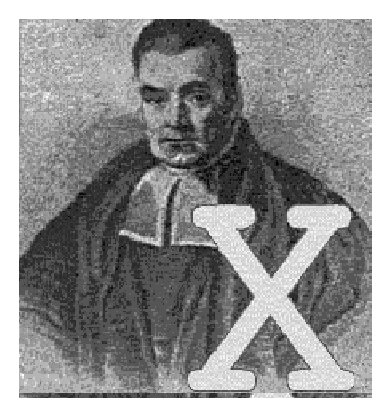
\includegraphics[scale=1.2]{grafiken/bayesicon.eps}
\end{center}
\end{figure}

\vfill

{\bf\sffamily \huge #1}

\vfill

\end{center}

{\em Developed by}

Christiane Belitz\\
Andreas Brezger\\
Nadja Klein (University of G\"{o}ttingen)\\
Thomas Kneib (University of G\"{o}ttingen)\\
Stefan Lang (University of Innsbruck) \\
Nikolaus Umlauf (University of Innsbruck) \\

\vspace{2ex}

{\em With contributions by}

\vspace{-1.5ex}

\begin{multicols}{2}
Daniel Adler\\
Paul Cochrane\\
Jan Fahrenholz\\
Eva-Maria Fronk\\
Felix Heinzl\\
Andrea Hennerfeind\\
Manuela Hummel\\
Alexander Jerak\\
Susanne Konrath\\
Petra Kragler\\
Cornelia Oberhauser\\
Leyre Est\'{\i}baliz Osuna Echavarr\'{\i}a\\
Daniel Saban\'{e}s Bov\'{e} \\
Achim Zeileis
\end{multicols}

{\em Supported by}

Ludwig Fahrmeir (mentally)\\
Leo Held (mentally)\\
German Research Foundation (DFG)

\newpage

\subsection*{Acknowledgements}

The development of {\em BayesX} has been supported by grants from the German Research Foundation (DFG), Collaborative
Research Center 386 ``Statistical Analysis of Discrete Structures''.

Special thanks go to (in alphabetical order of first names):

{\em Dieter Gollnow} for computing and providing the map of Munich (a really hard job); \\
{\em Leo Held} for advertising the program; \\
{\em Ludwig Fahrmeir} for his patience with finishing the program and for carefully
reading and correcting the  manual; \\
{\em Ngianga-Bakwin Kandala} for being the first user of the program (a really hard job); \\
{\em Samson Babatunde Adebayo} for carefully reading and correcting the manual; \\
{\em Ursula Becker} for carefully reading and correcting the manual;

\subsection*{Licensing agreement}

This program is free software; you can redistribute it and/or
modify it under the terms of the GNU General Public License
as published by the Free Software Foundation; either version 2
of the License, or (at your option) any later version.

This program is distributed in the hope that it will be useful,
but WITHOUT ANY WARRANTY; without even the implied warranty of
MERCHANTABILITY or FITNESS FOR A PARTICULAR PURPOSE.  See the
GNU General Public License for more details.

You should have received a copy of the GNU General Public License
along with this program; if not, write to the Free Software
Foundation, Inc., 51 Franklin Street, Fifth Floor, Boston, MA  02110-1301, USA.



\vspace{0.5cm}

{\em BayesX} is available at { \href{http://www.bayesx.org}{http://www.bayesx.org}}}


\chapter{What is BayesX?}

\begin{stanza}{General scope}

{\it BayesX} is a software tool for estimating structured additive
regression models. Structured additive regression embraces
several well-known regression models such as generalized additive
models (GAM), generalized additive mixed models (GAMM),
generalized geoadditive mixed models (GGAMM), dynamic models,
varying coefficient models, and geographically weighted regression
within a unifying framework. Besides exponential family
regression, {\em BayesX} also supports non-standard regression
situations such as regression for categorical responses, hazard
regression for continuous survival times, continuous time
multi-state models, quantile regression, distributional regression models and multilevel models.
\end{stanza}

\begin{stanza}{Inferential procedures}

Estimation of regression models can be achieved based on four
different inferential concepts that have been implemented in
separate regression objects:

\begin{itemize}
\item {\bf\sffamily MCMC simulation techniques (bayesreg objects):} A fully Bayesian interpretation of structured additive
    regression models is obtained by specifying prior distributions for all unknown parameters. Estimation can be
    facilitated using Markov chain Monte Carlo simulation techniques, a general and versatile concept for Bayesian
    inference. Bayesreg objects provide numerically efficient implementations of MCMC schemes for structured additive
    regression models in case of exponential family responses, categorical responses, hazard regression and multi-state models.
    Suitable proposal densities have been developed to obtain rapidly mixing, well-behaved sampling
    schemes without the need for manual tuning.
\item {\bf\sffamily MCMC simulation techniques (mcmcreg objects):} Mcmcreg objects provide similar functionality for fully Bayesian inference as bayesreg objects but implement distributional regression models for responses beyond simple exponential families (distributional regression), quantile regression and multilevel models. Generally, estimation is more efficient (in terms of computing time) than with bayesreg objects. Therefore mcmcreg objects should be preferred to bayesreg objects if possible.
\item{\bf\sffamily Mixed model based estimation (remlreg objects):} An increasingly popular way to estimate semiparametric
    regression models is the representation of penalisation approaches as mixed models. Within {\em BayesX }this concept
    has been extended to structured additive regression  models and several types of non-standard regression situations.
    The general idea is to take advantage of the close  connection between penalty concepts and corresponding random
    effects distributions. The smoothing parameters of the  penalties then transform to variance components in the random
    effects (mixed) model. While the selection of smoothing  parameters has been a difficult task for a long time, several
    estimation procedures for variance components in mixed models are already available since the 1970's. The most popular
    one is restricted maximum likelihood in Gaussian mixed models with marginal likelihood as the non-Gaussian counterpart.
    Remlreg objects employ mixed model methodology for the estimation of structured additive regression models. While
    regression coefficients are estimated based on penalised likelihood, restricted maximum likelihood or marginal
    likelihood estimation forms the basis for the determination of smoothing parameters. From a Bayesian perspective, this
    yields empirical Bayes / posterior mode estimates for the structured additive regression models. However, estimates can
    also merely be interpreted as penalised likelihood estimates from a frequentist perspective.
\item{\bf \sffamily Penalized least squares including model selection (stepwisereg objects):}
As a fourth alternative {\em BayesX} provides a penalized least squares (respectively penalized likelihood) approach for
estimating structured additive regression tools.
In addition to
the previously described estimation alternatives, a powerful variable and model selection tool is included.  Model choice and estimation of
the parameters is done simultaneously. The algorithms are able to
\begin{itemize}
\item decide whether a particular covariate enters the model,
\item decide whether a continuous covariate enters the model linearly or nonlinearly,
\item decide whether a spatial effect enters the model,
\item decide whether a unit- or cluster specific heterogeneity effect enters the model,
\item select complex interaction effects (two dimensional surfaces, varying coefficient terms),
\item select the degree of smoothness of  nonlinear covariate, spatial or cluster specific heterogeneity effects.
\end{itemize}
Inference is based on penalized likelihood in combination with fast
algorithms for selecting relevant covariates and model terms.
Different models are compared via various goodness of fit criteria,
e.g. AIC, BIC, GCV and 5 or 10 fold cross validation.
\end{itemize}
\end{stanza}


\begin{stanza}{Model classes and model terms}

{\em BayesX} provides functionality for the following types of
responses:

\begin{itemize}
\item{\bf\sffamily Univariate exponential family:} Supported response distributions are Gaussian, Poisson, Binomial and Gamma distribution as well as some simple versions of the
    negative binomial, zero-inflated Poisson, and zero-inflated negative binomial.

\item {\bf\sffamily Distributional regression:} A large number of univariate and multivariate continuous, discrete or mixed discrete-continuous responses can be treated within the framework of distributional regression. In this setting, potentially all parameters of these distributions can be related to structured additive predictors.

\item {\bf\sffamily Quantile Regression:} Bayesian quantile regression allows to study specific quantiles of the response distribution without relying on a specific distributional assumption.

\item{\bf\sffamily Categorical responses with unordered responses:} For categorical responses with unordered categories,
    {\em BayesX} supports multinomial logit and multinomial probit models. Both effects of category-specific and
    globally-defined covariates can be estimated. Category-specific offsets or non-availability indicators can be defined
    to account for varying choice sets.

\item{\bf\sffamily Categorical responses with ordered responses:} For ordered categorical responses, ordinal as well as
    sequential models can be specified. Effects can be requested to be category-specific or to be constant over the
    categories. Supported response functions include the logit and the probit transformation.

\item{\bf\sffamily Continuous time survival models:} {\em BayesX} supports Cox-type hazard regression models with
    structured additive predictor for continuous time survival analysis. In contrast to the Cox model, the baseline hazard
    rate is estimated jointly with the remaining effects based on penalized splines. Furthermore, both time-varying effects
    and time-varying covariates can be included in the predictor. Arbitrary combinations of right, left and interval
    censored as well as left truncated observations can be analysed.

\item{\bf\sffamily Continuous time multi-state models:} Multi-state models form a general class for the analysis of the
    evolution of discrete phenomena in continuous time. Transition intensities between the discrete states are specified in
    analogy to the hazard rate in continuous time survival models.
\end{itemize}

Structured additive regression models can be build from arbitrary
combinations of the following model terms:

\begin{itemize}
\item{\bf\sffamily Nonlinear effects:} Nonlinear effects can be estimated based on either penalised spline or random walk
    models.

\item{\bf\sffamily Seasonal effects:} Specific autoregressive priors allow for the estimation of flexible, time-varying
    seasonal effects.

\item{\bf\sffamily Spatial effects:} Spatial effects can be specified based on Markov random fields, stationary Gaussian
    random fields (kriging) or bivariate penalised splines. Both georeferenced regional data as well as point-referenced
    data based on coordinates are supported.

\item{\bf\sffamily Interaction surfaces:} Bivariate extensions of penalised splines allow to estimate flexible interactions
    between continuous covariates. Stationary Gaussian random fields can also be considered a radial basis function
    approach and, hence, form a second possibility for the specification of interaction surfaces.

\item{\bf\sffamily Varying coefficients:} Varying coefficient models with both continuous and spatial effect modifiers can
    be estimated. The latter case is also known as geographically weighted regression.

\item{\bf\sffamily Cluster-specific random effects:} {\em BayesX} supports i.i.d. Gaussian random intercepts and random
    slopes.

\item {\bf\sffamily Regularised high-dimensional effects:} High-dimensional vectors of regression coefficients can be
    assigned Bayesian regularisation priors. Available alternatives are ridge, lasso, and normal mixture of inverse gamma
    (spike and slab) priors.

\item {\bf\sffamily Multilevel models:} In multilevel models, parameters of specific effects can themselves be assigned a structured additive predictor (e.g. in multilevel random effects specifications).
\end{itemize}

Note that parts of the functionality may be available for one of the regression objects only. For example, bayesreg objects do
not support interval censored survival times while multinomial probit models can not be estimated with remlreg objects. Details
can be found in the chapters corresponding to the specific object types.
\end{stanza}

\begin{stanza}{Further functionality}

\begin{itemize}
\item{\bf\sffamily Handling and manipulation of data sets:} {\em
BayesX} provides a number of functions for handling and
manipulating data sets, e.g. for reading ASCII data sets, creating
new variables, obtaining summary statistics etc. Compare
\autoref{datasetobj} for details.

\item{\bf\sffamily Handling and manipulation of geographical
maps:} {\em BayesX} is able to manipulate and draw geographical
maps. The regions of the map may be colored according to some
numerical characteristics. In {\em BayesX} version 1.5, a new
color scheme based on HCL colors has been added to obtain a better
representation of colored maps independent of the display device.
Details can be found in \autoref{map} and \autoref{graphobj}.

\item{\bf\sffamily Visualizing data:} {\em BayesX} provides
functions for drawing scatter plots and geographical maps. A
number of additional options are provided to customize the graphs
according to the personal needs of the user. Details can be found
in \autoref{graphobj}.

\item{\bf\sffamily Model selection for Gaussian and non-Gaussian
dags:} This tool estimates Gaussian and non-Gaussian directed
acyclical graphs (dag) via reversible jump MCMC. Details can be
found in \autoref{dag}.
\end{itemize}
\end{stanza}

%\begin{stanza}{Recommendations for further reading}
%If you are interested in using {\em BayesX}, it is of course not
%necessary to read the complete manual. \autoref{recomm} provides a
%rough guideline for reading this manual and other sources,
%depending on the features of {\em BayesX} you are interested in
%and your statistical background. In any case, you should read
%sections \ref{availableversions} -- \ref{generalusage} to make
%yourself familiar with the general usage of {\em BayesX}.

%\begin{table}[ht] \footnotesize
%\hspace{1cm}\begin{tabular}{ |p{7cm}|p{7.7cm}|}
% \hline
% {\bf Intended use and background} & {\bf Guideline} \\
% \hline\hline
% Bayesian semiparametric regression based on MCMC
% simulation techniques. No experience with MCMC.
% & Read an introductory text about MCMC first. A brief introduction is given
% for example in \citeasnoun{Gre01}. Read the methodology manual to make yourself
% familiar with STAR models.
% Proceed with chapter \ref*{zambiaanalysis} of the tutorial manual. \\
% \hline Bayesian semiparametric regression based on MCMC simulation
% techniques. At least basic knowledge about MCMC.
% & Read the methodology manual to make yourself familiar with STAR
% models. Proceed with chapter \ref*{zambiaanalysis} of the tutorial manual. \\
% \hline
% Semiparametric regression based on mixed model methodology. &
% Read the methodology manual to make yourself familiar with STAR
% models. Proceed with chapter \ref*{remlregzambiaanalysis} of the tutorial manual. \\
%\hline
%Semiparametric regression based on penalized least squares including
%variable and model selection. &
% Read the methodology manual to make yourself familiar with STAR
% models. Proceed with chapter \ref*{zambia_step_analysis} of the tutorial manual. \\
% \hline Model selection for DAGs. No experience with reversible jump
% MCMC. & Read an introductory text about reversible jump MCMC first.
% A brief introduction is given for example in \citeasnoun{Gre01}. Proceed with \autoref{dag}. \\
% \hline
% Draw and color geographical maps & Read \autoref{map} and \autoref{graphdrawmap} of the reference manual. \\
% \hline
%\end{tabular}
%\begin{center}
%{\em \caption {\label{recomm} Recommendations for further
%reading.}}
%\end{center}
%\end{table}
%\end{stanza}


\chapter{Getting started}
\label{gettingstarted}

This chapter provides some useful information for first-time users
of {\em BayesX}: Which versions of BayesX are currently available
(\autoref{availableversions}), how is BayesX installed
(\autoref{installbayesx}), what types of manuals exist
(\autoref{bayesxmanuals}), and how is the graphical user interface
organized (\autoref{bayesxwindows}). Section \ref{generalusage}
describes the general usage of {\em BayesX} and the structure of
{\em BayesX} syntax. The final section contains a description of
three data sets that will be used for demonstrating purposes in
the later chapters.

\section{Available versions of BayesX}
\label{availableversions} \index{Java based version} \index{non-Java
based version} \index{versions} \index{versions!Java based}
\index{versions!non-Java based}

In its current form, {\em BayesX} runs only under the various
versions of the Windows operating system (e.g. Windows 95, 98,
2000, NT, XP). The graphical user interface and the visualisation
tools are implemented in Java, while the computerintensive parts
of the program have been implemented in C++. The current version
of {\em BayesX} can be downloaded from
\href{http://www.stat.uni-muenchen.de/~bayesx}
{http://www.stat.uni-muenchen.de/\~{}bayesx}.

Up to version 1.3, {\em BayesX} has been distributed in two
versions, the {\em Java based version} described above and a {\em
non-Java based version}, which was written completely in C++.
Since the Java based version has additional features, the non-Java
based version is no longer supported.

\section{Installing BayesX}\label{installbayesx}
\index{installation} \index{installation directories}

After you have downloaded the file #installBayesX.exe# from the
{\em BayesX} homepage, proceed by executing this file. The
installation process is quite simple and comparable to most
standard installations. The installation routine will request all
necessary information.

When {\em BayesX} has been installed successfully, it can be
started using the {\em Windows Start} button or the icon created
on the desktop (depending on your specifications during the
installation process). The installation directory contains the
five subdirectories #doc#, #examples#, #output#, #sfunctions# and
#temp#. The #doc# directory contains the program documentation,
i.e. the three {\em BayesX} manuals (see the following
subsection). The #examples# directory contains the three data
sets, #credit.raw#, #rents.raw# and #zambia.raw#, which will be
used for demonstrating purposes throughout the manual. A detailed
description of these data sets is given in
\autoref{datadescription}. The #examples# directory also contains
some tutorial programs that illustrate the usage of {\em BayesX},
see the tutorials manual. The #output# directory is the default
directory for program output stored in files. Of course, the
output window can be redefined by the user, compare
\autoref{bayesregglobopt} and \autoref{remlregglobopt}. The
#sfunctions# directory contains some R and S-plus functions for
visualizing estimation results obtained with {\em bayesreg
objects} or {\em remlreg objects}, see \autoref{splus} for a
detailed description of these functions. Note, however, that the
current {\em BayesX} version has its own graphics capabilities,
see \autoref{graphobj} and \autoref{visualization} for details.
Finally, temporary files created when estimating regression models
will be stored in the #temp# directory. Usually you will never use
this directory.

The subdirectories and their content are briefly summarized in
\autoref{dirtable}.

\begin{table}[ht]
\begin{center}
\begin{tabular}{|l|l|}
\hline
Directory & Content \\
\hline
#doc# & the {\em BayesX} manuals \\
#examples# & data set examples and tutorial programs \\
#output# & default directory for estimation output \\
#sfunctions# & R and S-plus functions for visualizing output \\
#temp# & temporary files \\
\hline
\end{tabular}
{\em\caption{ \label{dirtable} Subdirectories of the installation
directory and their content.}}
\end{center}
\end{table}

\section{Manuals}\label{bayesxmanuals}
\index{Manuals}

{\em BayesX} is shipped with three different manuals. The
reference manual (i.e. the manual you are just reading) gives
detailed information on the general usage of BayesX, the syntax of
{\em BayesX} commands and the different objects used by {\em
BayesX}. The methodology manual provides background information on
the statistical methodology that is implemented in {\em BayesX}.
In this manual you will also find more references on the
methodological background. The tutorial manual is intended to make
new users familiar with the usage of {\em BayesX} by demonstrating
examples. It contains two self-contained tutorials, describing how
to perform semiparametric regression analyses using {\em BayesX}.
The manuals are also available from the help menu and can be found
in the #doc# directory (a subdirectory of the installation
directory).

\section{Windows and buttons in BayesX}\label{bayesxwindows}
\index{windows}

After starting {\em BayesX} you will see a main window with a menu
bar and four additional subwindows. The four windows are the {\em
command window}, the {\em output window}, the {\em review window}
and the {\em object browser}. The purpose of these windows is
described in the following four subsections. Below the menu bar
there is a menu bar containing the buttons BREAK, PAUSE and
SUPPRESS OUTPUT, and the priority menu. Their functionality is
described in subsection \ref{buttons} and \ref{prioritymenu}.

\subsection{The command window}
\index{command window} \index{windows!command}

Allmost all {\em BayesX} commands are entered and executed in the
{\em command window}. By default, a command will be executed if
you press the return key. You can change this default delimiter
using the #delimiter# command, see \autoref{delimiter}.

\subsection{The output window}
\index{output window} \index{windows!output}

In the {\em output window}, all commands entered in the {\em
command window} or executed through a batch file (see
\autoref{batch}) are printed together with the program output.

\index{saving the output} The content of the {\em output window}
can be saved and processed with your favorite text editor. For
saving the output, enter the {\em file menu} and click on {\em
Save output} or {\em Save output as}. The file save dialog will
allow you to choose between two different file formats. The
default is the rich-text format but it is also possible to store
the {\em output window} in plain ASCII format. This, however, has
the disadvantage that all text highlights (for example bold
letters) will disappear in the saved file.

The {\em file menu} also allows to clear the {\em output window}
(i.e. delete the content of the window) or to open an already
existing file.

Depending on the screen resolution of your computer, letters
appearing in the {\em output window} may be very small or too
large. The font size can be varied in the {\em preferences menu}.

\subsection{The review window}
\index{review window} \index{windows!review}

In many cases, subsequent commands change only slightly. The {\em
review window} gives you convenient access to the last 100 past
commands entered during a session. Double click on one of these
past commands and it is automatically copied to the {\em command
window}, where it can be modified and / or executed again.

\subsection{The object browser}
\index{object browser}

{\em BayesX} is object oriented, i.e. different types of objects
are used to store data, estimate regression models, etc. The {\em
object browser} provides an overview of the objects currently
defined and about their contents. The {\em object browser} window
is split into two parts. The left part displays the different
object types currently supported by {\em BayesX} ({\em dataset
objects}, {\em bayesreg objects}, {\em remlreg objects}, {\em map
objects}, {\em dag objects} and {\em graph objects})s. By clicking
on one of the object types, the names of all objects of this type
will appear in the right panel of the {\em object browser}. Double
clicking on one of the names gives a visualization of the object
and / or a short summary in the {\em output window}, depending on
the object type. Double clicking on {\em dataset objects}, for
example, will open a spreadsheet where the variables and the
observations of the data set can be inspected. Clicking on {\em
map objects} opens a window that contains a graphical
representation of the map.

\subsection{BREAK, PAUSE and SUPPRESS OUTPUT button}
\label{buttons} \index{PAUSE button} \index{BREAK button}
\index{SUPPRESS OUTPUT button} \index{buttons}
\index{buttons!PAUSE} \index{buttons!BREAK}
\index{buttons!SUPPRESS OUTPUT}

The {\em BayesX} button panel contains the BREAK button, the PAUSE
button and the SUPPRESS OUTPUT button. The purpose of the BREAK
button is to interrupt the process that is currently executed
(this may take some time). Clicking on the PAUSE button interrupts
the current process temporarily until the button is pressed again.
If a process is paused, the button caption PAUSE is replaced by
CONTINUE, indicating that a second click on the button will
continue the current process. Pausing a current process will
increase the execution speed of other programs currently running
on your computer. Clicking the SUPPRESS OUTPUT button suppresses
printing of output in the {\em output window}. The button caption
changes to SHOW OUTPUT to indicate that an additional click on the
button will cause the program to print the output again.
Suppressing the output increases the execution speed of {\em
BayesX} and saves memory. Note, that you can store your output in
a log-file even if printing of the output is suppressed (see
\autoref{logfile}).

\subsection{Priority menu}
\label{prioritymenu} \index{Priority menu}

When running extensive computations, it may be desirable to reduce
the priority of BayesX since otherwise all further programs may be
executed very slowly. The priority menu allows you to change the
priority of your computations from within BayesX. Usually there
should be no need to increase the priority (although it is
possible). To pause the current computations use the PAUSE button.

\section{General usage of BayesX}
\label{generalusage}

\subsection{Creating objects}
\label{createobject} \index{objects} \index{objects!create}

{\em BayesX} is implemented in an object oriented way, although
the object oriented concept does not go too far, i.e. inheritance
or other concepts of object oriented programming languages such as
S or C++ are not supported. As a consequence, the first thing to
do during a session, is to create some objects. Currently, six
different object types are available: {\em dataset objects}, {\em
bayesreg objects}, {\em remlreg objects}, {\em map objects}, {\em
dag objects} and {\em graph objects}. {\em Dataset objects} are
used to store, handle, and manipulate data sets, see
\autoref{datasetobj} for details. {\em Map objects} are used to
handle geographical information and are covered in more detail in
\autoref{map}. The main purpose of {\em map objects} is to serve
as auxiliary objects for {\em bayesreg objects} or {\em remlreg
objects} when estimating spatial effects. {\em Graph objects} are
used to visualize data (e.g. to create scatterplots or to color
geographical maps according to some numerical characteristics),
see \autoref{graphobj} for details. The most important object
types are {\em bayesreg objects} and {\em remlreg objects}. These
objects are used to estimate Bayesian semiparametric regression
models based on either Markov Chain Monte Carlo simulation
techniques ({\em bayesreg objects}) or a mixed model
representation of the regression model ({\em remlreg objects}).
See \autoref{bayesreg} for a detailed description of {\em bayesreg
objects} and \autoref{remlreg} for a detailed description of {\em
remlreg objects}. {\em Dag objects} are used to estimate Gaussian
or non-Gaussian DAGs (direct acyclic graphs) based on reversible
jump MCMC simulation techniques (see \autoref{dag} for details).

The syntax for creating a new object is:

#># {\em objecttype objectname}

To create for example a {\em dataset object} with name #mydata#, simply type:

#> dataset mydata#

Note that some restrictions are imposed on the names of objects,
i.e. not all object names are allowed. For example, object names
have to begin with an uppercase or lowercase letter rather than a
number. Section \ref{varnames} discusses valid variable names but
the same rules apply also to object names.

\subsection{Applying methods to previously defined objects}

When an object has been created successfully, you can apply
methods to that particular object. For instance, {\em dataset
objects} may be used to read data stored in an ASCII file using
method #infile#, to create new variables using method #generate#,
to modify existing variables using method #replace# and so on. The
syntax for applying methods to the objects is similar for all
methods and independent of the particular object type. The general
syntax is: \index{general syntax} \index{syntax}

#># {\em objectname.methodname} [{\em model}] [#weight# {\em varname}] [#if# {\em boolean expression}] [, {\em options}] \\
\hspace*{4.8cm} [#using# {\em usingtext}]

\autoref{syntaxtable} explains the syntax parts in more detail.


\begin{table}[ht]
 \centering
\begin{tabular}{|l|l|}
\hline
Syntax part & Description \\
\hline
{\em objectname} & the name of the object to apply the method to \\
{\em methodname} & the name of the method \\
{\em model} & a model specification (for example a regression model) \\
{\em #weight# varname} & specifies {\em varname} as weight variable \\
#if# {\em boolean expression} & indicates that the method should be applied only if a \\
& certain condition holds \\
, {\em options} & define (or modify) options for the method \\
#using# {\em usingtext} & indicates that another object or file is required to \\
& apply the particular method \\
\hline
\end{tabular}
{\em \caption{\label{syntaxtable}Parts of the general BayesX
syntax.}}
\end{table}

Note that $[\dots]$ indicates that this part of the syntax is
optional and may be omitted. Moreover for most methods only some
of the syntax parts above will be meaningful. The specification of
invalid syntax parts is not allowed and will cause an error
message.

We illustrate the concept with some simple methods of {\em dataset
objects}. Suppose that a {\em dataset object} with name #mydata#
has already been created and that some variables should be
created. First of all, we have to tell {\em BayesX} how many
observations we want to create. This can be done with the
 #set obs# command, see also \autoref{setobs}. For example

#> mydata.set obs = 1000#

indicates that the data set #mydata# should have 1000
observations. In this case, the {\em methodname} is #set# and the
{\em model} is #obs =# #1000#. Since no other syntax parts (for
example #if# statements) are meaningful for this method, they are
not allowed. For instance, specifying an additional weight
variable #x# by typing

#> mydata.set obs = 1000 weight x#

will cause the error message:

#ERROR: weight statement not allowed#

In a second step we can now create a new variable #X#, say, that
contains Gaussian (pseudo) random numbers with mean 2 and standard
deviation 0.5:

#> mydata.generate X = 2+0.5*normal()#

Here, #generate# is the {\em methodname} and #X = 2+0.5*normal()#
is the {\em model}. In this case the {\em model} consists of the
specification of the new variable name, followed by the equal sign
'#=#' and a mathematical expression for the new variable. Similar
as for the #set obs# command other syntax parts are not meaningful
and therefore not allowed. If the negative values of #X# should be
replaced with the constant 0, this can be achieved using the
#replace# command:

#> mydata.replace X = 0 if X < 0#

Obviously, the #if# statement is meaningful and is therefore
allowed, but not required.

\section{Description of data set examples}
\label{datadescription} \index{data set examples}

This section describes three data sets used to illustrate many of
the features of {\em BayesX} in the following chapters as well as
in the tutorial manual. All data sets are stored columnwise in
plain ASCII-format. The first row of each data set contains the
variable names separated by blanks. Subsequent rows contain the
observations, one observation per row.

\subsection{Rents for flats}
\label{rentdata} \index{rents for flats} \index{data set
examples!rents for flats}

According to the German rental law, owners of apartments or flats
can base an increase in the amount that they charge for rent on
'average rents' for flats comparable in type, size, equipment,
quality and location in a community. To provide information about
these 'average rents', most of the larger cities publish 'rental
guides', which can be based on regression analyses with rent as
the dependent variable. The file #rent94.raw# (stored in the
#examples# directory) is a subsample of data collected in 1994 for
the Munich rental guide. The variable of primary interest is the
monthly rent per square meter in German Marks. Covariates
characterizing the flat were constructed from almost 200 variables
out of a questionnaire answered by tenants of flats. The present
data set contains a small subset of these variables that are
sufficient for demonstration purposes (see \autoref{rentdatavar}).

In addition to the data set, the #examples# directory contains a
map of Munich in the file #munich.bnd#. This map will be useful
for visualizing effects of the location #L#. See \autoref{map} for
a description on how to incorporate geographical maps into {\em
BayesX}.

\begin{table}

\centering
\begin{tabular}{|l|l|}
\hline
{\bf Variable} & {\bf Description} \\
\hline
R & monthly rent per square meter in German marks \\
$F$ & floor space in square meters \\
$A$ & year of construction \\
$L$ & location of the building in subquarters \\
 \hline
\end{tabular}
{\em \caption{\label{rentdatavar}Variables of the rent data set.}}
\end{table}


\subsubsection*{References}

\begin{description}

\item[Lang, S. and Brezger, A. (2004):]
\href{http://www.stat.uni-muenchen.de/~lang/publications.html}
{Bayesian P-splines.} {\it Journal of Computational and Graphical
Statistics}, 13, 183-212.

\end{description}


\subsection{Credit scoring}
\label{creditdata} \index{credit scoring} \index{data set
examples!credit scoring}

The aim of credit scoring is to model and / or predict the
probability that a client with certain covariates ('risk factors')
will not pay back his credit. The data set contained in the file
#credit.raw# consists of 1000 consumer credits from a bank in
southern Germany. The response variable is 'creditability' in
dichotomous form ($y=0$ for creditworthy, $y=1$ for not
creditworthy). In addition, 20 covariates that are assumed to
influence creditability were collected. The present data set
(stored in the #examples# directory) contains a subset of these
covariates that proved to be the main influential variables on the
response variable, see Fahrmeir and Tutz (2001, ch. 2.1).
\autoref{creditdatavar} gives a description of the variables of
the data set. Usually a binary logit model is applied to estimate
the effect of the covariates on the probability of being not
creditworthy. As in the case of the rents for flats example, this
data set is used to demonstrate the usage of certain features of
{\em BayesX}, see primarily \autoref{creditanalyse} for a Bayesian
regression analysis of the data set.

\begin{table}[ht]

\begin{tabular}{|l|l|}
\hline
{\bf Variable} & {\bf Description} \\
\hline
$y$ & creditability, dichotomous with $y=0$ for creditworthy, $y=1$ for \\
    & not creditworthy \\
$account$ & running account, trichotomous with categories "no
running account" \\& ($=1$),
    "good running account"
($=2$),  "medium running account" \\&("less than 200 DM") ($=3$)  \\
$duration$ & duration of credit in months, continuous \\
$amount$ & amount of credit in 1000 DM, continuous \\
$payment$ & payment of previous credits, dichotomous with categories "good" ($=1$), \\ & "bad" ($=2$)  \\
$intuse$ & intended use, dichotomous with categories "private" ($=1$) or \\ & "professional" ($=2$)  \\
$marstat$ & marital status, with categories "married" ($=1$) and "living alone" ($=2$). \\
\hline
\end{tabular}
{\em \caption{\label{creditdatavar}Variables of the credit scoring
data set.}}
\end{table}

\subsubsection*{References}

\begin{description}
\item [Fahrmeir, L., Tutz, G. (2001):] {\it Multivariate Statistical
Modelling based on Generalized Linear Models.} New York:
Springer--Verlag.
\end{description}

\subsection{Childhood undernutrition in Zambia}
\label{zambia} \index{childhood undernutrition} \index{data set
examples!childhood undernutrition}

Acute and chronic undernutrition is considered to be one of the
worst health problems in developing countries. Undernutrition
among children is usually determined by assessing the
anthropometric status of the child relative to a reference
standard. In our example undernutrition is measured through
stunting (insufficient height for age), indicating chronic
undernutrition. Stunting for child $i$ is determined using the
Z-score
\[Z_i = \frac{AI_i-MAI}{\sigma}\]
where $AI$ refers to the child`s anthropometric indicator (height
at a certain age in our example), MAI refers to the median of the
reference population and $\sigma$ refers to the standard deviation
of the reference population.

The data set #zambia.raw# contains the (standardized) Z-score for
4847 children together with several covariates that are supposed
to influence undernutrition (e.g. the body mass index of the
mother, the age of the child, and the district the mother lives
in). \autoref{zambiavar} gives more information on the covariates
in the data set.

This data set is used in chapter \ref*{zambiaanalysis} and
\ref*{remlregzambiaanalysis} of the tutorial manual.

\begin{table}[|h|t|]
\begin{center}
\begin{tabular}{|l|l|}
 \hline
 {\bf Variable} & {\bf Description}\\
 \hline
 $hazstd$ & standardized Z-score for stunting\\
 $bmi$ & body mass index of the mother\\
 $agc$ & age of the child\\
 $district$ & district where the mother lives\\
 $rcw$ & mother`s employment status with categories "working" (= 1) and "not working" \\
 & (= $-1$)\\
 $edu1$ & mother`s educational status with categories "complete primary but incomplete\\
 $edu2$ & secondary" ($edu1=1$), "complete secondary or higher" ($edu2=1$) and\\
 & "no education or incomplete primary" ($edu1=edu2=-1$)\\
 $tpr$ & locality of the domicile with categories "urban" (= 1) and "rural" (= $-1$)\\
 $sex$ & gender of the child with categories "male" (= 1) and
 "female" (= $-1$)\\
 \hline
\end{tabular}
{\em\caption{Variables in the undernutrition data set.
\label{zambiavar}}}
\end{center}
\end{table}

\subsubsection*{References}

\begin{description}
\item [Kandala, N. B., Lang, S., Klasen, S. and Fahrmeir, L. (2001):] Semiparametric Analysis of
the Socio-Demographic and Spatial Determinants of Undernutrition
in Two African Countries.{\it Research in Official Statistics}, 1,
81-100.
\end{description}


\chapter{Special Commands}

This chapter describes some commands that are not associated with
a particular object type. Among others, there are commands for
exiting {\em BayesX}, opening and closing log files, saving
program output, deleting objects etc.

\section{Exiting BayesX}
\index{exiting BayesX}

You can exit {\em BayesX} by typing either

#> exit#

or

#> quit#

in the {\em command window}. Of course, {\em BayesX} can also be
closed using the 'exit' entry from the file menu or by clicking on
the cross in the upper right corner.

\section{Opening and closing log files} \label{logfile}
\index{log files}

Program output and commands entered by the user can automatically
be stored in a log file to make them available for editing in your
favorite text editor. Another important application of log files
is the documentation of your work. A log file is opened by the
command:

#> logopen# [{\em, option}] #using# {\em filename}

Afterwards all commands entered and all program output will be
saved in the file {\em filename}. If the log file specified in
{\em filename} is already existing, new output is appended at the
end of the file. To overwrite an existing log file, option
#replace# has to be specified in addition. Note that it is not
allowed to open more than one log file simultaneously.

An open log file can be closed by typing:

#> logclose#

Exiting {\em BayesX} automatically closes the current log file.

\section{Saving the contents of the output window}
\index{output window!saving the contents} \index{saveoutput}

You can save the contents of the {\em output window} not only with
the {\em file$\rightarrow$save output} or {\em
file$\rightarrow$save output as} menu, but also using the
#saveoutput# command. This is particularly useful for automatic
saving in batch files, see \autoref{batch}. The syntax for saving
the {\em output window} is

#> saveoutput# [{\em , options}] #using# {\em filename}

where {\em filename} is the file (including path) in which the
contents of the output will be stored.

\subsection*{Options}

\begin{itemize}
\item # replace# \\
By default an error will be raised if you try to store the
contents of the {\em output window} in a file that is already
existing. This preserves you from overwriting a file
unintentionally. An already existing file can be overwritten by
explicitly specifying the #replace# option.
\item #type = rtf #$|$# txt # \\
The {\em output window} can be saved in two different file types,
namely rich text format (the default) and plain ASCII (requested
by specifying #type=txt# as an option.
\end{itemize}

\section{Changing the delimiter}
\label{delimiter} \index{delimiter}

By default, commands entered using the {\em command window} will
be executed after pressing the return key. This can be
inconvenient, in particular if your statements are long or in
batch files. In this case it may be favorable to split a statement
into several lines, and execute the command using a different
delimiter.

You can change the delimiter using the #delimiter# command. The
syntax is

#> delimiter# = {\em newdel}

where {\em newdel} is the new delimiter. Only two different
delimiters are currently allowed, namely the return key and the
'#;#' (semicolon) key. To specify the semicolon as the delimiter,
type

#> delimiter = ;#

and press return. To return to the return key as the delimiter, type

#> delimiter = return;#

Note that this statement has to end with a semicolon, since this
was previously set to be the current delimiter.


\section{Using batch files}
\label{batch} \index{batch files}

You can execute commands stored in a file just as if they were
entered from the keyboard. This may be useful if you want to
re-run a certain analysis more than once (possibly with some minor
changes) or if you want to run time consuming statistical methods.

Execution of a batch file is started by typing

#> usefile# {\em filename}

This executes the commands stored in {\em filename} successively.
{\em BayesX} will not stop the execution if an error occurs in one
or more commands. Note that it is allowed to invoke another batch
file within a currently running batch file.


\subsubsection*{Comments}\index{comments}

Comments in batch files are indicated by a  #%#
sign, i.e. every line
starting with #%# is ignored by the program.

\subsubsection*{Changing the delimiter}

In particular in batch files, the readability of your program code
may be improved if some (long) commands are split up into several
lines. By default this will cause errors, because {\em BayesX}
interprets each line in your program as one statement. To overcome
this problem one has to change the delimiter using the #delimiter#
command, see \autoref{delimiter}.

\section{Dropping objects}
\index{objects!dropping} \index{dropping objects}

You can delete objects by typing

#> drop# {\em objectlist}

This drops the objects specified in {\em objectlist}. The names of
the objects in {\em objectlist} must be separated by blanks.


\chapter{dataset objects} \label{chap_data}
\label{datasetobj} \index{dataset objects} \index{dataset}

{\em Authors: Stefan Lang, Christiane Belitz and Manuela Hummel}   \\
{\em email: \href{mailto:lang@stat.uni-muenchen.de}{lang@stat.uni-muenchen.de}}\\
\vspace{0.3cm}


{\em Dataset objects} are used to manage and manipulate data. A new {\em dataset object} is created by typing

#> dataset# {\em objectname}

where {\em objectname} is the name of the data set. After the
creation of a {\em dataset object} you can apply the methods for
manipulating and managing data sets discussed below.

Note that in the current version of {\em BayesX} {\bf only
numerical variables are allowed}. Hence, string valued variables,
for example,  are not yet supported by {\em BayesX}.

\section{Method descriptive}
\label{descriptive} \index{summary statistics}
\index{descriptives} \index{dataset!descriptive command}

\subsection*{Description}

Method #descriptive# calculates and displays univariate summary
statistics. The method computes the number of observations, the
mean, median, standard deviation, minimum and maximum of
variables.

\subsection*{Syntax}

#> #{\em objectname}.#descriptive# {\em varlist} [#if# {\em expression}]

Method #descriptive# computes summary statistics for the variables
in {\em varlist}. An optional #if# statement may be added to
analyze only a part of the data.

\subsection*{Options}

not allowed

\subsection*{Examples}

The statement

#> d.descriptive x y#

computes summary statistics for the variables #x# and #y#.
The statement

#> d.descriptive x y if x>0#

restricts the analysis to observations with #x>0#.


\section{Method drop}
\label{drop} \index{dropping variables} \index{dropping
observations} \index{dataset!drop command}

%\bigskip
%{\bf \em  Description} \\

\subsection*{Description}

Method #drop# deletes variables or observations from the data set.

%\bigskip
\subsection*{Syntax}

#> #{\em objectname}.#drop# {\em varlist}

#> #{\em objectname}.#drop if# {\em expression}

The first command may be used to eliminate the variables specified
in {\em varlist} from the data set. The second statement may be
used to eliminate certain observations. An observation will be
removed from the data set if {\em expression} is true, i.e. the
value of the expression is one.

\subsection*{Options}

not allowed

\subsection*{Examples}

The statement

#> credit.drop account duration#

drops the variables #account# and #duration# from the credit scoring data set. With the statement

#> credit.drop if  marstat = 2#

all observations with #marstat=2#, i.e. all persons living alone,
will be dropped from the credit scoring data set.
The following statement

#> credit.drop account duration if marstat = 2#

will raise the error

#ERROR: dropping variables and observations in one step not allowed#

It is not allowed to drop variables and certain observations in
one single command.


\section{Functions and Expressions}
\label{expression} \index{expressions}

The primary use of expressions is to generate new variables or
change existing variables, see \autoref{generate} and
\autoref{replace}, respectively. Expressions may also be used in
#if# statements to force {\em BayesX} to apply a method only to
observations where the boolean expression in the #if# statement
is true. The following are all examples of expressions:

#2+2# \\
#log(amount)# \\
#1*(age <= 30)+2*(age > 30 & age <= 40)+3*(age > 40)# \\
#age=30# \\
#age+3.4*age^2+2*age^3# \\
#amount/1000#


\subsection{Operators}
\index{expressions!operators} \index{operators}


{\em BayesX} has three different types of operators: arithmetic,
relational and logical. Each of the types is discussed below.

\subsubsection{Arithmetic operators}
\index{operators!arithmetic}

The arithmetic operators are #+# (addition), #-# (subtraction),
#*# (multiplication), #/# (division), #^# (raise to a power) and
the prefix #-# (negation). Any arithmetic operation on a missing
value or an impossible arithmetic operation (such as division by zero) yields a missing value.

{\bf Example}

The expression

#(x+y^(3-x))/(x*y)#

denotes the formula

$$
\frac{x+y^{3-x}}{x\cdot y}
$$

and evaluates to missing if #x# or #y# is missing or zero.


\subsubsection{Relational operators}
\index{operators!relational}

The relational operators are #># (greater than), #<# (less than),
#>=# (greater than or equal), #<=# (less than or equal), #=#
(equal) and #!=# (not equal). Relational expressions are either
1 (i.e. the expression is true) or 0 (i.e. the expression is false).



{\bf Examples}

Relational operators may be used to create indicator variables.
The following statement generates a new variable #amountcat# (out
of the already existing variable #amount#), whose
value is 1 if #amount<=10# and 2 if #amount>10#.

#> credit.generate amountcat = 1*(amount<=10)+2*(amount>10)#

Another useful application of relational operators is in #if#
statements. For example, changing
an existing variable only when a certain condition holds can be done by the following command:

#> credit.replace amount = NA if amount <= 0#

This sets all observations missing where #amount<=0#.

\subsubsection{Logical operators}
\index{operators!logical}

The logical operators are #&# (and) and #|# (or).

{\bf Example}

Suppose you want to generate a variable #amountind# whose value is
1 for married people with
amount greater than 10 and 0 otherwise. This can be done by typing

#> credit.generate amountind = 1*(marstat=1 & amount > 10)#


\subsubsection{Order of evaluation of the operators}
\index{operators!order of evaluation}

The order of evaluation (from first to last) of operators is

#^# \\
#/#, #*#\\
#-#, #+#\\
#!=#, #>#, #<#, #<=#, #>=#, #=#\\
#&#, #|#.

Brackets may be used to change the order of evaluation.


\subsection{Functions}
\index{functions}

Functions may appear in expressions. Functions are indicated by
the function name, an opening and a closing parenthesis. Inside
the parentheses one or more arguments may be specified. The
argument(s) of a function may be any expression, including other
functions. Multiple arguments are separated by commas. All
functions return missing values when given missing values as
arguments or when the result is undefined.


\bigskip
{\bf Functions reference}

\autoref{mathfunc} references all mathematical functions;
\autoref{statfunc} references all statistical functions.
\index{functions!abs} \index{functions!cos} \index{functions!sin}
\index{functions!exp} \index{functions!floor}
\index{functions!lag} \index{functions!logarithm}
\index{functions!square root} \index{functions!bernoulli
distributed random numbers} \index{functions!binomial distributed
random numbers} \index{functions!cumulative distribution function}
%\index{Functions!gamma distributed random numbers}
\index{functions!exponential distributed random numbers}
\index{functions!normally distributed random numbers}
\index{functions!uniformly distributed random numbers}


\begin{table}[ht]
\begin{center}
\begin{tabular}{|l|l|}
\hline
{\bf Function} & {\bf Description} \\
\hline \hline
abs(x) & absolute value \\
cos(x) & cosine of radians \\
exp(x) & exponential \\
floor(x) & returns the integer obtained by truncating $x$. \\
& Thus floor(5.2) evaluates to 5 as floor(5.8). \\
lag(x) & lag operator \\
log(x) & natural logarithm \\
log10(x) & log base 10 of $x$ \\
sin(x) & sine of radians \\
sqrt(x) & square root \\
\hline
\end{tabular}
{\em\caption{\label{mathfunc} List of mathematical functions.}}
\end{center}
\end{table}



\begin{table}[ht]
\begin{center}
\begin{tabular}{|l|p{11cm}|}
\hline
{\bf Function} & {\bf Description} \\
\hline \hline bernoulli($p$) & returns Bernoulli distributed
random numbers with probability of success $p$. If $p$ is not
within the interval $[0;1]$, a
 missing value will be returned. \\
\hline binomial($n,p$) & returns $B(n;p)$ distributed random
numbers. Both, the number of trials $n$ and the probability of
success $p$ may be expressions. If $n < 1$, a missing value will
be returned. If $n$ is not integer valued, the number of trials
will be $[n]$. If $p$ is not within the interval $[0;1]$, a
missing value will be returned. \\
\hline
cumul($x$) & cumulative distribution function \\
\hline
cumulnorm($x$) & cumulative distribution function $\Phi$ of the standard normal distribution. \\
\hline exponential($\lambda$) & returns exponentially distributed
random numbers with parameter $\lambda$.
If $\lambda \leq 0$, a missing value will be returned. \\
\hline gamma($\mu$,$\nu$) & returns gamma distributed random
numbers with mean $\mu$ and variance $\mu^2/ \nu$.
If $\mu$ and/or $\nu$ are less than zero, a missing value will be returned.  \\
\hline normal() & returns standard normally distributed random
numbers;
$N(\mu,\sigma^2)$ distributed random numbers may be generated with $\mu + \sigma$*normal(). \\
\hline uniform() & uniform pseudo random number function; returns
uniformly distributed
pseudo-random numbers on the interval $(0,1)$ \\
\hline
\end{tabular}
{\em \caption{\label{statfunc} List of statistical functions}}
\end{center}
\end{table}


\subsection{Constants}
\index{expressions!constants} \index{number of observations}
\index{missing values} \index{$\pi$} \index{current observation}

\autoref{constant} lists all constants that may be used in expressions.


\begin{table}[ht]
\begin{center}
\begin{tabular}{|l|l|}
\hline
Constant & Description \\
\hline \hline
\texttt{\_n} & contains the number of the current observation.  \\
\texttt{\_N }& contains the total number of observations in the data set. \\
\texttt{\_pi} & contains the value of $\pi$. \\
\texttt{NA} & indicates a missing value \\
.  & indicates a missing value \\

\hline
\end{tabular}
{\em \caption{\label{constant} List of constants}}
\end{center}
\end{table}


{\bf Examples}

The following statement generates a variable #obsnr# whose value
is 1 for the first observation, 2 for the second and so on.

#> credit.generate obsnr = _n#

The command

#> credit.generate nrobs = _N#

generates a new variable {\em nrobs} whose values are equal to the
total number of observations, say 1000, for all observations.

\subsection{Explicit subscribing}
\index{expressions!explicit subscribing} \index{subscribing}

Individual observations on variables can be referenced by
subscribing the variables. Explicit subscripts are specified by
the variable name with square brackets that contain an expression.
The result of the subscript expression is truncated to an integer,
and the value of the variable for the indicated observation is
returned. If  the value of the subscript expression is less than 1
or greater than the number of observations in the data set,
a missing value is returned.

{\bf Examples}

Explicit subscribing combined with the constant #_n# (see
\autoref{constant}) can be used to create lagged values
on a variable. For example the lagged value of a variable #x# in a data set #data# can be created by

#> data.generate xlag = x[_n-1]#

\newpage

Note that #xlag# can also be generated using the #lag# function

#> data.generate xlag = lag(x)#


\section{Method generate}
\label{generate} \index{generating new variables}
\index{dataset!generate command}

\subsection*{Description}

#generate# is used to create a new variable.


\subsection*{Syntax}

#> #{\em objectname}.#generate# {\em newvar} = {\em expression}

Method #generate# creates a new variable with name {\em newvar}.
See \autoref{varnames} for valid variable names. The values of the
new variable are specified by {\em expression}. The details of
valid expressions are covered in \autoref{expression}.


\subsection*{Options}

not allowed


\subsection*{Examples}

The following command generates a new variable called #amount2#
whose values are the square of amount in the credit
scoring data set.

#> credit.generate amount2 = amount^2#

If you try to change the variable currently generated, for example by typing

#> credit.generate amount2 = amount^0.5#

the error message

#ERROR: variable amount2 is already existing #

will occur. This prevents you to change an existing variable
unintentionally. An existing variable may be changed with method
#replace#, see \autoref{replace}.

If you want to generate an indicator variable #largeamount# whose
value is 1 if #amount# exceeds a certain value, say 3.5, and 0
otherwise, the following will
produce the desired result:

#> credit.generate largeamount = 1*(amount>3.5)#


\section{Method infile}
\label{infile} \index{reading data from ASCII files}
\index{dataset!infile command}


\subsection*{Description}

Reads in data saved in an ASCII file.


\subsection*{Syntax}

#> #{\em objectname}.#infile #[{\em varlist}] [{\em , options}] #using# {\em filename}

Reads in data stored in {\em filename}. The variables are given
names specified in {\em varlist}. If {\em varlist} is empty, i.e.
there is no {\em varlist} specified, it is assumed that the first
row of the datafile contains the variable names separated by
blanks or tabs. It is not required that the observations in the
datafile are stored in a special format, except that successive
observations should be separated by one or more blanks (or tabs).
The first value read from the file will be the first observation
of the first variable, the second value will be the first
observation of the second variable, and so on. An error will occur
if for some variables no values can be read for the last
observation.

It is assumed that  a period '.' or 'NA' indicates a missing
value.

Note that in the current version of {\em BayesX} {\bf only
numerical variables are allowed}. Thus, the attempt to read in
string valued variables, for example, will cause an error.


\subsection*{Options}

\begin{itemize}
\item {\bf missing = missingsigns} \\
By default a dot '.' or 'NA' indicates a missing value. If you
have a data set where missing values are indicated by different
signs than '.' or 'NA', you can force {\em BayesX} to recognize
these signs as missing values by specifying the #missing# option.
For example #missing = MIS# defines MIS as an indicator for a
missing value. Note that
 '.' and 'NA' remain valid indicators for missing values, even if the missing
option is specified.

\item {\bf maxobs = integer} \\
If you work with large data sets, you may observe the problem that
reading in a data set using the #infile# command is very time
consuming. The reason for this problem is that {\em BayesX} does
not know the number of observations and thus the memory needed in
advance. The effect is that new memory must be allocated whenever
a certain amount of memory is used. To avoid this problem the
#maxobs# option may be used, leading to a considerable reduction
of computing time. This option forces {\em BayesX} to allocate in
advance enough memory  to store at least {\em integer}
observations before new memory must be reallocated. Suppose for
example that your data set consists approximately of 100,000
observations. Then specifying #maxobs = 105000# allocates enough
memory to read in the data set quickly. Note that #maxobs = 105000#
does not mean that your data set cannot hold more than
105,000 observations. This means only that new memory will/must be
allocated when the number of observations of your data set exceeds
the 105,000 observations limit.
\end{itemize}


\subsection*{Examples}

Suppose we want to read a data set stored in
#c:\data\testdata.raw# containing two
variables #var1# and #var2#.
The first few rows of the datafile could look like this:

var1 var2 \\
2 2.3 \\
3 4.5 \\
4 6 \\
...


To read in this data set, we first have to create a new {\em dataset
object}, say #testdata#, and then read the data using
the #infile# command. The following two commands will produce the desired result.

#> dataset testdata# \\
#> testdata.infile using c:\data\testdata.raw#

If the first row of the data set file contains no variable names,
the second command must be modified to:

#> testdata.infile var1 var2 using c:\data\testdata.raw#

Suppose furthermore that the data set you want to read in is a
pretty large data set with 100,000
observations. In that case the #maxobs# option is very useful to reduce reading time.  Typing for example

#> testdata.infile var1 var2 , maxobs=101000 using c:\data\testdata.raw#

will produce the desired result.


\section{Method outfile}
\label{outfile} \index{writing data to a file} \index{saving data
in an ASCII file} \index{dataset!outfile command}

\subsection*{Description}

Method #outfile# writes data to a disk file in ASCII format. The saved
data can be read back using the #infile# command, see
\autoref{infile}.



\subsection*{Syntax}

#> #{\em objectname}.#outfile# [{\em varlist}] [#if# {\em expression}] [{\em , options}] #using# {\em filename}

#outfile# writes the variables specified in {\em varlist} to the
disk file with name {\em filename}. If {\em varlist} is omitted in
the outfile statement, {\em all} variables in the data set are
written to disk. Each row in the data file corresponds to one
observation. Different variables are separated by blanks.
Optionally, an #if# statement may be used to write only those
observations to disk where a certain boolean expression, specified
in {\em expression}, is true.


\subsection*{Options}


\begin{itemize}
\item {\bf header} \\
Specifying the #header# option forces {\em BayesX} to write the
variable names in the first row of the created data file.
\item {\bf replace} \\
The #replace# option allows {\em BayesX} to overwrite an already
existing data file. If #replace# is omitted in the option list and
the file specified in {\em filename} is already existing, an error
will be raised.
This prevents you from overwriting an existing file unintentionally.
\end{itemize}


\subsection*{Examples}

The statement

#> credit.outfile using c:\data\cr.dat#

writes the complete credit scoring data set to
#c:\data\cr.dat#. To generate two different
ASCII
data sets for married people and people living alone, you could type

#> credit.outfile if marstat = 1 using c:\data\crmarried.dat# \\
#> credit.outfile if marstat = 2 using c:\data\cralone.dat#

Suppose you only want to write the two variables #y# and #amount#
to disk. You could type

#> credit.outfile y amount using c:\data\cr.dat#

This will raise the error message

#ERROR: file c:\data\cr.dat is already existing#

\newpage

because #c:\data\cr.dat# has already been created. You can
overwrite the file using the #replace# option

#> credit.outfile y amount , replace using c:\data\cr.dat#


\section{Method pctile}
\label{pcitle} \index{percentiles of variables}
\index{dataset!pctile command}

\subsection*{Description}

Method #pctile# computes and displays the
1\%,5\%,25\%,50\%,75\%,95\% and 99\%  percentiles of a variable.

\subsection*{Syntax}

#># {\em objectname}.#pctile# {\em varlist} [#if# {\em expression}]

Method #pctile# computes and displays the percentiles of the
variables specified in {\em varlist}. An optional #if# statement
may be added to compute the percentiles only for a part of the
data.

\subsection*{Options}

not allowed

\subsection*{Examples}

The statement

#> d.pctile x y#

computes percentiles for the variables #x# and #y#.
The statement

#> d.pctile x y if x>0#

restricts the analysis to observations with x$>$0.


\section{Method rename}
\index{renaming variables} \index{dataset!rename command}


\label{rename}


\subsection*{Description}

#rename# is used to change variable names.


\subsection*{Syntax}

#> #{\em objectname}.#rename# {\em varname} {\em newname}

#rename# changes the name of {\em varname} to {\em newname}. {\em
newname} must be a valid variable name, see \autoref{varnames} on
how to create valid variable names.

\bigskip
{\bf Options}

not allowed



\section{Method replace}
\label{replace} \index{changing existing variables}
\index{dataset!replace command}



\subsection*{Description}

#replace# changes the values of an existing variable.


\subsection*{Syntax}

#> #{\em objectname}.#replace# {\em varname} = {\em expression} [#if# {\em boolexp}]

#replace# changes the values of the existing variable {\em
varname}. If {\em varname} is not existing, an error will be
raised. The new values of the variable are specified in {\em
expression}. Expressions are covered in \autoref{expression}. An
optional #if# statement may be used to change the values of the
variable only if the boolean expression {\em boolexp} is true.


\subsection*{Options}

not allowed


\subsection*{Example}

The statement

#> credit.replace amount = NA if amount<0#

changes the values of the variable #amount# in the credit scoring
data set to missing if #amount<0#.


\section{Method set obs}
\label{setobs}


\subsection*{Description}

#set obs# changes the current number of observations in a data
set.


\subsection*{Syntax}

#> #{\em objectname}.#set obs# = {\em intvalue}

#set obs# raises the number of observations in the data set to
{\em intvalue}, which must be greater or equal to the current
number of observations. This prevents you from deleting parts of
the data currently in memory. Observations may be eliminated using
the #drop# statement, see \autoref{drop}. The values of the
additionally created observations will be set to the missing
value.



\section{Method sort}
\label{sort} \index{sorting variables} \index{dataset!sort
command}


\subsection*{Description}

Sorts the data set.


\subsection*{Syntax}

#> #{\em objectname}.#sort# {\em varlist}  [{\em , options}]

Sorts the data set with respect to the variables specified in {\em
varlist}. Missing values are interpreted to be larger than any
other number and are thus placed last.


\subsection*{Options}

\begin{itemize}
\item {\bf descending}  \\
If this option is specified, the data set will be sorted in
descending order. The default is ascending order.
\end{itemize}


\section{Method tabulate}
\label{tabulate} \index{tabulate} \index{table of frequencies}
\index{one way table of frequencies} \index{dataset!tabulate
command}

\subsection*{Description}

Method #tabulate# calculates and displays a frequency table for a
variable.

\subsection*{Syntax}

#># {\em objectname}.#tabulate# {\em varlist} [#if# {\em expression}]

Method #tabulate# computes and displays frequency tables of the
variables specified in {\em varlist}. An optional #if# statement
may be added to restrict the analysis to a part of the data.

\subsection*{Options}

not allowed

\subsection*{Examples}

The statement

#> d.tabulate x y#

displays  frequency tables for the variables #x# and #y#.
The statement

#> d.tabulate x y if x>0#

restricts the analysis to observations with #x>0#.


\section{Variable names}
\label{varnames} \index{variables names}


A valid variable name is a sequence of letters (#A#-#Z# and #a#-#z#),
digits (#0#-#9#), and underscores (#_#). The first character of a
variable name must  either be a letter or an underscore. {\em
BayesX} respects upper and lower case letters, that is #myvar#,
#Myvar# and #MYVAR# are three distinct variable names.


\section{Examples}

This section contains two examples on how to work with {\em
dataset objects}. The first example illustrates some of the
methods described above, using one of the example data sets stored
in the #examples# directory, the credit scoring data set. A
description of this data set can be found in \autoref{creditdata}.
The second example shows how to simulate complex statistical
models.

\subsection{The credit scoring data set}

In this section we illustrate how to code categorical variables
according to one of the coding schemes, dummy or effect coding.
This will be useful in regression models, where all categorical
covariates must be coded in dummy or effect coding before they can
added to the model.

We first create a {\em dataset object} #credit# and read in the data using the #infile# command.

#> dataset credit# \\
#> credit.infile using c:\bayes\examples\credit.raw#

We can now generate new variables to obtain dummy coded versions
of the categorical covariates
#account#, #payment#, #intuse# and #marstat#:

#> credit.generate account1  = 1*(account=1)# \\
#> credit.generate account2  = 1*(account=2)# \\
#> credit.generate payment1 = 1*(payment=1)# \\
#> credit.generate intuse1 = 1*(intuse=1)# \\
#> credit.generate marstat1 = 1*(marstat=1)#

The reference categories are chosen to be 3 for #account# and 2
for the other variables. Alternatively, we could code the
variables according to effect coding. This is achieved with the
following program code:

#> credit.generate account_eff1  = 1*(account=1)-1*(account=3)# \\
#> credit.generate account_eff2  = 1*(account=2)-1*(account=3)# \\
#> credit.generate payment_eff1 = 1*(payment=1)-1*(payment=2)# \\
#> credit.generate intuse_eff1 = 1*(intuse=1)-1*(intuse=2)# \\
#> credit.generate marstat_eff1 = 1*(marstat=1)-1*(marstat=2)#


\subsection{Simulating complex statistical models}
\index{dataset!simulation of} \index{simulation of artificial data
sets}

In this section we illustrate how to simulate complex regression
models. Suppose first we want to simulate data according to the
following Gaussian regression model:

\begin{eqnarray}
y_i & = & 2 + 0.5 x_{i1} + \sin(x_{i2}) + \epsilon_i, \quad i = 1,\dots,1000 \\
x_{i1} & \sim & U(-3,3) \quad i.i.d.  \\
x_{i2} & \sim & U(-3,3) \quad i.i.d.  \\
\epsilon_i & \sim & N(0,0.5^2) \quad i.i.d.
\end{eqnarray}

We first have to create a new data set #gsim#, say, and specify the desired number of observations:

#> dataset gsim# \\
#> gsim.set obs = 1000#

In a second step the covariates #x1# and #x2# have to be created. In
this first example we
assume that the covariates are uniformly distributed between -3 and 3. To generate them, we must type:

#> gsim.generate x1 = -3+6*uniform()# \\
#> gsim.generate x2 = -3+6*uniform()#

In a last step we can now create the response variable by typing

#> gsim.generate y = 2 + 0.5*x1+sin(x2)+0.5*normal()#

You could now (if you wish) estimate a Gaussian regression model
with the generated data set using one of the regression tools of {\em BayesX}, see
\autoref{bayesreg} or \autoref{remlreg}. Of course, more refined models could be
simulated. We may for example drop the assumption of a constant
variance of $0.5^2$ in the error term. Suppose the variance is
heteroscedastic and growing with order log($i$)
where $i$ is the observation index. We can simulate such a heteroscedastic model by typing:

#> gsim.replace y = 2 + 0.5*x1+sin(x2)+0.1*log(_n+1)*normal()#

In this model the standard deviation is

$$
\sigma_i = 0.1*\log(i+1), \quad  i = 1,\dots,1000.
$$

Suppose now that we want to simulate data from a logistic
regression model. In a logistic regression model it is assumed
that (given the  covariates) the response variable $y_i$,
$i=1,\dots,n$, is binomially distributed with parameters $n_i$ and
$\pi_i$ where $n_i$ is the number of replications and $\pi_i$ is
the probability of success. For $\pi_i$ one assumes that it is
related to a linear predictor $\eta_i$ via the logistic
distribution function, that is

$$
\pi_i = \frac{\exp(\eta_i)}{1+\exp{(\eta_i)}}.
$$

To simulate such a model we have to specify the linear predictor
$\eta_i$ and the number of replications $n_i$. We specify a
similar linear predictor as in the example above for Gaussian
response, namely

$$
\eta_i = -1+0.5x_{i1}-\sin(x_{i2}).
$$


For simplicity, we set $n_i=1$ for the number of replications. The
following commands generate a data set 'bin'
according to the specified model:


#> dataset bin #\\
#> bin.set obs = 1000# \\
#> bin.generate x1 = -3+6*uniform()# \\
#> bin.generate x2 = -3+6*uniform()# \\
#> bin.generate eta = -1+0.5*x1-sin(x2)# \\
#> bin.generate pi = exp(eta)/(1+exp(eta))# \\
#> bin.generate y = binomial(1,pi)#

Note that the last three statements can be combined into a single command:

#> bin.generate y = binomial(1,exp(-1+0.5*x1-sin(x2))/(1+exp(-1+0.5*x1-sin(x2)))#


The first version however is much easier to read and should
therefore be preferred.


\chapter{map objects}
\label{map} \index{map object}


{\em Authors: Stefan Lang and Andreas Brezger} \\
{\em email: \href{mailto:stefan.lang@stat.uni-muenchen.de}{stefan.lang@stat.uni-muenchen.de} and \href{mailto:andib@stat.uni-muenchen.de}{andib@stat.uni-muenchen.de}}\\
\vspace{0.3cm}


{\em Map objects} are used to handle and store geographical maps.
For the moment {\em map objects} serve more or less as auxiliary
objects for {\em bayesreg objects} and {\em remlreg objects},
where the effect of spatial covariates on a dependent variable can
be modelled via spatial priors, especially Markov random field
priors. The main purpose of {\em map objects} in this context is
to provide the neighborhood structure of the map and to compute
weights associated with this neighborhood structure. The typical
approach is as follows: A {\em map object} is created and the
boundary information of a geographical map is read from an
external file and stored in the {\em map object}. This can be
achieved using the #infile# command, see \autoref{mapinfile}
below. Based on the boundary information, the {\em map object}
automatically computes the neighborhood structure of the map and
the weights associated with the neighborhood structure. Since
there are several proposals in the spatial statistics literature
for defining the weights, the user is given the choice between a
couple of alternative weight definitions. After the correct
initialization, the {\em map object} can be passed to the
#regress# function of a {\em bayesreg object} in order to estimate
regression models with spatial covariates, see \autoref{bayesreg}
and \autoref{remlreg}, and the subsections about spatial
covariates therein.

\clearpage



\section{Method infile}
\label{mapinfile} \index{map object!infile command} \index{map
object!boundary files} \index{boundary files} \index{graph files}
\index{reading graph files} \index{reading boundary files}

\subsection{Description}


Method #infile# is used to read the boundary information of a
geographical map stored in an external file. This file is called a
{\em boundary file}, since it must contain the information about
the boundaries of the different regions of the map. It is assumed
that the boundary of each region is stored in form of a closed
polygon, that is the boundary is represented by a set of connected
straight lines. A detailed description of the structure of
boundary files is given below.

As a second choice method #infile# allows to read  so called {\em
graph files}. In {\em graph files} the nodes and edges of a
certain graph are stored. In addition, weights associated with the
edges of the graph may be specified in the file. In terms of
geographical maps the nodes of a graph correspond to the regions
of a map and the edges specify the neighborhood structure of the
map. The main advantage of {\em graph files} is that the
neighborhood structure of a particular geographical map is already
available. With {\em boundary files} the neighborhood structure
must be computed first; a task which is relatively computer
intensive. Therefore an advisable strategy might be to read a {\em
boundary files} only once to compute the neighborhood structure
and to store it as a {\em graph file} afterwards using the
#outfile# command (see \autoref{mapoutfile}), especially for
geographical maps with a lot of regions. However, using {\em graph
files} also has a disadvantage: Visualization of geographical
information is only possible with boundary files since only these
contain the required information on the boundaries.

\subsection{Syntax}

#> #{\em objectname}.#infile# [{\em , options}] #using# {\em filename}

Method #infile# reads the map information stored in the {\em
boundary} or {\em graph file} {\em filename}. If option #graph# is
specified, {\em BayesX} expects a {\em graph file}, otherwise a
{\em boundary file}
is expected. The structures of {\em boundary} and {\em graph files} are described below.

\subsubsection*{Structure of a boundary file}

A {\em boundary file} provides the boundary information of a
geographical map. For each region of the map the {\em boundary
file} must contain the identifying name of the region, the
polygons that form the boundary of the region, and the number of
lines the polygon consists of. The first line always contains the
region code surrounded by quotation marks and the number of lines
the polygon of the region consists of. The code and the number of
lines must be separated by a comma. The subsequent lines contain
the coordinates of the straight lines that form the boundary of
the region. The straight lines are represented by the coordinates
of their end points. Coordinates must be separated by a comma.

To give an example we print a (small) part of the {\em boundary
file} of Germany:


\footnotesize

\hspace{1cm}  $\vdots$

"6634",31 \\
2319.26831,4344.48828 \\
2375.45435,4399.50391 \\
2390.67139,4446.32520 \\
2470.26807,4405.35645 \\
2576.78735,4379.60449 \\
2607.22144,4337.46533 \\
2627.12061,4356.19385 \\
2662.23682,4355.02344 \\
2691.50024,4311.71338 \\
2726.61646,4310.54248 \\
2716.08154,4256.69775 \\
2710.22900,4227.43408 \\
2680.96533,4234.45752 \\
2583.81055,4165.39551 \\
2568.59351,4096.33398 \\
2520.60132,4042.48901 \\
2535.81836,3941.82251 \\
2490.16724,3920.75269 \\
2451.53955,3903.19458 \\
2437.49292,3924.26440 \\
2369.60156,3933.62866 \\
2359.06665,3951.18677 \\
2285.32275,3969.91553 \\
2258.40015,4061.21753 \\
2197.53223,4049.51221 \\
2162.41602,4086.96948 \\
2204.55542,4091.65161 \\
2192.85010,4125.59717 \\
2284.15210,4220.41113 \\
2339.16748,4292.98438 \\
2319.26831,4344.48828

\hspace{1cm} $\vdots$

\normalsize

\vspace{0.3cm}

The  map corresponding to the section of the {\em boundary file}
above can be found in \autoref{partgermany}. Note that the first
and the last point must be identical (see the example above) to
obtain a closed polygon.


\begin{figure}[ht]
\centering
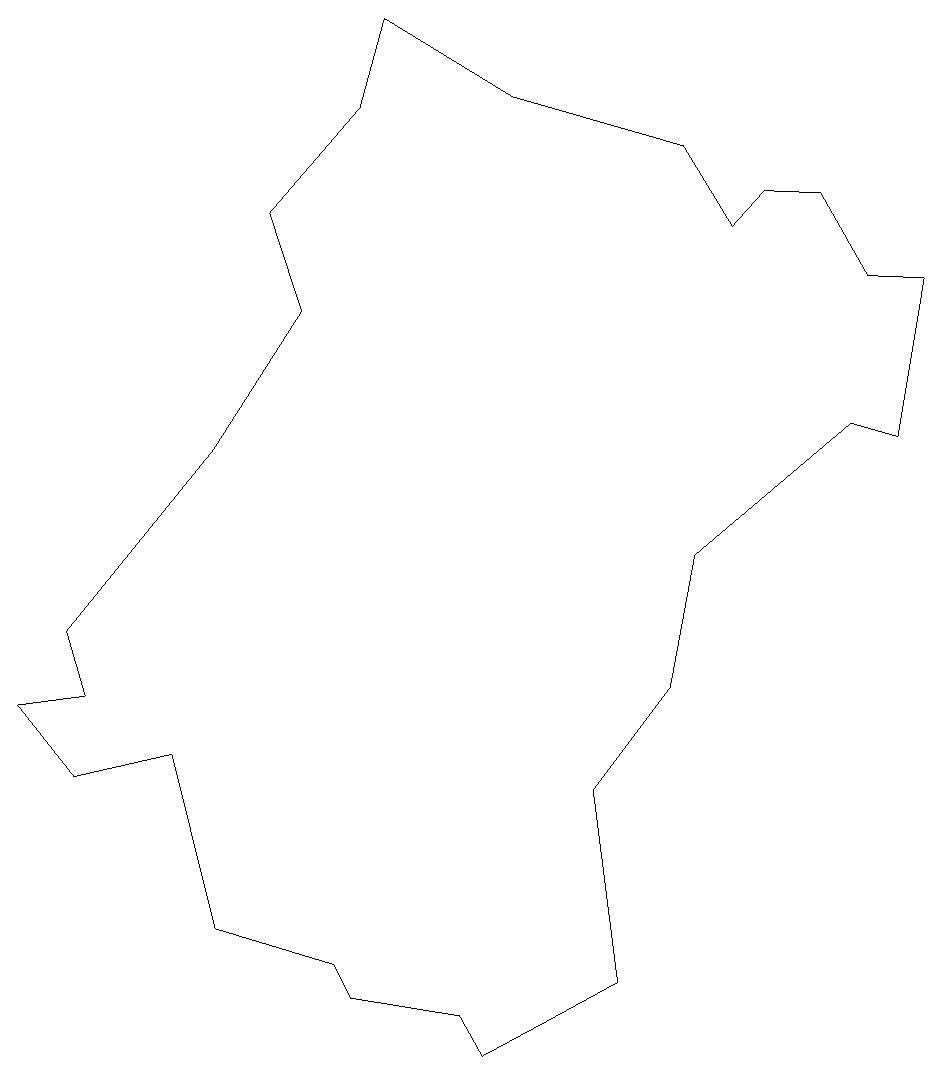
\includegraphics [scale=0.3]{grafiken/westpart.eps}
{\em\caption{\label{partgermany} Corresponding graph of the
section of the boundary file}}
\end{figure}

In some cases it might happen that a region is separated into
subregions that are not connected. As an illustrative example
compare \autoref{westsub} showing a region of Germany that is
separated into 8 subregions. In this case the {\em boundary file}
must contain the polygons of all subregions. The first row for
each of these subregions must contain the region code and the
number of lines the polygon of the respective subregion consists
of. Note that it is not necessary that the polygons of the
subregions are stored in subsequent order in the {\em boundary
file}.

Another special case that might occur is illustrated in
\autoref{westin}. Here a region is completely surrounded by
another region. In this case an additional line must be added to
the boundary description of the {\em surrounded} region. The
additional line must be placed  after the first line and must
contain the
region code of the {\em surrounding} region. The syntax is:

#is.in#,"{\em region code}"

The following lines show a section of the {\em boundary file} of
Germany, where region "9361" is totally
surrounded by region "9371":

\footnotesize

\hspace{1cm} $\vdots$

"9361",7 \\
is.in,"9371" \\
4155.84668,2409.58496 \\
4161.69922,2449.38330 \\
4201.49756,2461.08862 \\
4224.90820,2478.64673 \\
4250.66016,2418.94922 \\
4193.30371,2387.34448 \\
4155.84668,2409.58496

\hspace{1cm} $\vdots$

\normalsize

\begin{figure}[hb]
\centering

\includegraphics [scale=0.3]{grafiken/reg1054.eps}
{\em\caption{\label{westsub} Example for a region that is divided
into subregions}}
\end{figure}

\begin{figure}[hb]
\centering
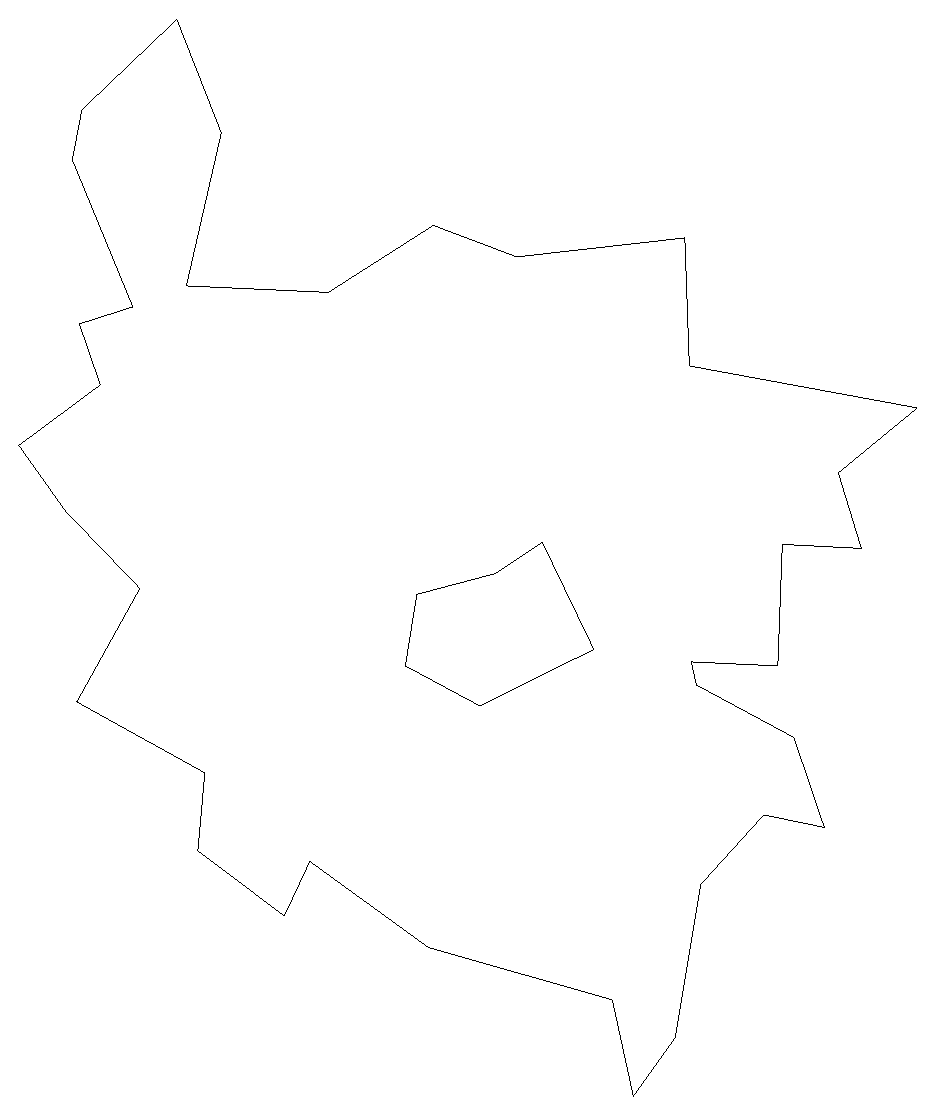
\includegraphics [scale=0.3]{grafiken/westin.eps}
{\em\caption{\label{westin} Example for a region that is totally
surrounded by another region}}
\end{figure}



Finally, we want to draw attention to an important limitation in
the current version of {\em BayesX}. In most cases {\em map
objects} serve as auxiliary objects to estimate spatial effects
with {\em bayesreg objects} or {\em remlreg objects}. In this case the names of the regions
of the map and the values of the spatial covariate, whose effect
is estimated, must match. Since there are only numerical variables
allowed in {\em dataset objects} (and no string valued variables),
the names of the regions in the corresponding {\em map object}
must necessarily be numbers, although there is in principle no
limitation for the names of regions in {\em map objects}.

\subsubsection*{Structure of a graph file}

A graph file stores the nodes and the edges of a graph $G =
(N,E)$, see for example George and Liu (1981, Ch. 3) for a first
introduction into graph theory. A graph is a convenient way of
representing the neighborhood structure of a geographical map. The
nodes of the graph correspond to the region codes. The
neighborhood structure is represented by the edges of the graph.
In some situations it may be useful to define weights associated
with the edges of a graph which can be stored in the {\em graph
file} as well.

We now describe the structure of a {\em graph file} as it is expected by
{\em BayesX}. The first line of a {\em graph file} must contain
the total number of nodes of the graph. In the remaining lines,
the nodes of the graph together with their edges and associated
weights are specified. One node corresponds to three consecutive
lines. The first of the three lines must contain the name of the
node, which may simply be the name of a geographical region. In
the second line the number of edges of that particular node is
given. The third line contains the corresponding edges of the
node, where an edge is given by the index of a neighboring node.
The index starts with zero. For example, if the fourth and the
seventh node/region in the {\em graph file} are
connected/neighbors, the edge index for the fourth node/region is
6 and for the seventh node/region 3.

We illustrate the structure of a {\em graph file} with an example. The
following few lines are the beginning
of the {\em graph file} corresponding to the map of (former) West Germany:

\footnotesize

327 \\
9162 \\
3 \\
1 2 3 \\
9174 \\
6 \\
0 4 2 3 5 6 \\
9179 \\
6 \\
0 1 7 3 8 6

\hspace{1cm} $\vdots$

\normalsize

\vspace{0.5cm}

The first line specifies the total number of nodes, in the present
example 327 nodes. The subsequent three lines correspond to the
node with name '9162', which is the first region in the map of
West Germany. Region '9162' has 3 neighbors, namely the second,
third and fourth node appearing in the graph file. Once again,
note that the index starts with zero, i.e. 0 corresponds to the
first node, 1 corresponds to the second node and so on. Lines 5 to
7 in the example correspond to node '9174' and its neighbors and
lines 8 to 10 correspond to node '9179'.

In a {\em graph file} it is also possible to specify weights associated
with the edges of the nodes. Since in the preceding example no
weights are explicitly specified, all weights are automatically
defined to be equal to one. Nonequal weights are specified in the
{\em graph file} by simply adding them following the edges of a
particular node.
An example of the beginning of a {\em graph file} with weights is given below:

\footnotesize

327 \\
9162 \\
3 \\
1 2 3 0.4 1.2 0.7\\
9174 \\
6 \\
0 4 2 3 5 6 0.4 0.3 0.8 0.8 1.4 1.6\\
9179 \\
6 \\
0 1 7 3 8 6 1.2 0.8 0.2 1.8 1.7 1.3

\hspace{1cm} $\vdots$

\normalsize

\vspace{0.5cm}

Here the edges of the first node '9162' have weights 0.4, 1.2 and
0.7.\bigskip



\subheader{Options}

\begin{itemize}
\item #graph# \\
If #graph# is specified as an additional option, {\em BayesX}
expects a {\em graph file} to be read in rather than a {\em
boundary file}.
\item #weightdef=adjacency# $|$ #centroid#  $|$ #combnd# \\
\label{weightsmap} Option #weightdef# allows to specify how the
weights associated with each pair of neighbors are computed.
Currently there are three weight specifications available,
#weightdef=adjacency#, #weightdef=centroid# and
#weightdef=combnd#. If #weightdef=adjacency# is specified, for
each pair of neighbors the weights are set equal to one. The so
called adjacency weights are the most common ones in spatial
statistics. Specifying #weightdef=centroid# results in weights
proportional to the distance of the centroids of neighboring
regions. More specifically, the weight $w_{us}$ of two neighboring
regions $u$ and $s$ is set to $w_{us} = c \cdot \exp(-d(u,s))$,
where $d$ is the Euclidian distance between the centroids of the
two sites and $c$ is a normalizing constant. The constant $c$ is
chosen in such a way that the total sum of weights is equal to the
total number of neighbors, which is in analogy to adjacency
weights. The third choice #weightdef=combnd# results in weights
proportional to the length of the common boundary. Similarly to
#weightdef=centroid#, the weights are normalized, i.e. the total
sum of weights is equal to the number of neighbors.

Note that the specification of the #weightdef# option is only
meaningful if a {\em boundary file} is read. If a {\em graph file}
is read  instead, the option has no effect because the boundary
information of regions is missing and  the computation of weights
is therefore impossible.
\end{itemize}



\clearpage



\section{Method outfile}
\label{mapoutfile} \index{map object!outfile command}

\begin{stanza}{Description}

{Method #outfile# performs the reverse of the #infile# command.
Using method #outfile#, the map information currently in memory is
written to an external file. The map information can be written
either in {\em boundary file} or in {\em graph file} format.}
\end{stanza}

\begin{stanza}{Syntax}

{#># {\em objectname}.#outfile# [{\em , options}] #using# {\em
filename}

#outfile# writes the map information to the external file
specified in {\em filename}. The file format can be either a {\em
boundary file} or a {\em graph file}. If #graph# is specified as
an additional option, the file format will be a {\em graph file},
otherwise a {\em boundary file}.}
\end{stanza}

\subheader{Options}

\begin{itemize}
\item #graph# \\
Forces the program to store the map information in {\em graph
file} format rather than {\em boundary file} format.
\item #includeweights# \\
Option #includeweights# is meaningful only if the storing format
is a {\em graph file}, i.e. option #graph# is additionally
specified. In that case the weights associated with the edges
(neighbors) of the nodes (regions) are additionally stored.
\item #replace# \\
The #replace# option allows {\em BayesX} to overwrite an already
existing file. If #replace# is omitted in the optionlist and the
file specified in {\em filename} already exists, an error will be
raised. This prevents you from overwriting an existing file
unintentionally.
\end{itemize}



\clearpage



\section{Method reorder}
\label{mapreorder} \index{reorder regions of a map} \index{map
object!reorder command}

\begin{stanza}{Description}

{Method #reorder# reorders the regions of a map in the sense that
the adjacency matrix of the reordered map has the smallest
envelope when compared to all other possible orderings. A new map
should always be reordered before using it with {\em bayesreg
objects} because MCMC updates for spatial covariates will be much
faster if the envelope of the posterior precision matrix is small.
For reordering of the regions of the map the reverse Cuthill
Mc-Kee algorithm is used, see George and Liu (1981) p. 58 ff.}
\end{stanza}

\begin{stanza}{Syntax}

{#># {\em objectname}.#reorder#

#reorder# reorders the regions of a map in order to obtain
smallest envelope of the corresponding adjacency matrix.}
\end{stanza}

\begin{stanza}{Options}

{Not allowed.}
\end{stanza}

\begin{stanza}{Reference}

{\begin{description}

\item[George, A., Liu, J. W. (1981).] {\em Computer Solution of Large
Sparse Positive Definite Systems.} Series in computational
mathematics, Prentice--Hall.

\end{description}}
\end{stanza}


\chapter{graph objects}
\label{graphobj} \index{Graph object} \index{Visualizing data}

{\em Graph objects} are used to visualize data or estimation
results obtained with the regression objects in {\em BayesX}.
Currently, {\em graph objects} can be used to draw scatterplots
between variables (\autoref{graphplot}, method #plot#), or to draw
and color geographical maps stored in {\em map objects}
(\autoref{graphdrawmap}, method #drawmap#). The resulting plots
are either printed on the screen or stored as postscript files for
further use in other documents (e.g. \LaTeX\/ documents). A {\em
graph object} is created by typing

#> graph# {\em objectname}

in the {\em command window}.


\clearpage


\section{Method drawmap}
\label{graphdrawmap} \index{Graph object!Drawmap command}
\index{Drawing geographical maps}

\begin{stanza}{Description}

Method #drawmap# is used to draw geographical maps and color the
regions according to some numerical characteristics.
\end{stanza}

\begin{stanza}{Syntax}

 #> #{\em objectname}.#drawmap#  [{\em plotvar regionvar}] [#if# {\em expression}], {\em #map#=mapname} [{\em options}]\\
 #> #[#using# {\em dataset}]

Method #drawmap# draws the map stored in the {\em map object} {\em
mapname} and prints the graph either on the screen or stores it as
a postscript file (if option #outfile# is specified). The regions
with regioncode {\em regionvar} are colored according to the
values of the variable {\em plotvar}. The variables {\em plotvar}
and {\em regionvar} are supposed to be stored in the {\em dataset
object} {\em dataset}. An #if# statement may be specified to use
only a part of the data in {\em dataset}. Several options are
available, e.g. for changing from grey scale to color scale or to
store the map as a postscript file. See the options list below for
more details.
\end{stanza}

\begin{stanza}{Options}

The most important option, which therefore is obligatory, is the
#map# option. This option specified the name of the {\em map
object} containing the boundary information to be drawn.
Additional options for method #drawmap# (in alphabetical order)
are:
\end{stanza}

\begin{itemize}
\item #color#

The #color# option allows to choose between a grey scale and a
colored scale. If the keyword #color# is specified, a colored
scale is used instead of a grey scale.

\item #drawnames#

In some situations it may be useful to print the names of the
regions into the graph (although the result will probably be
confusing in most cases). This can be achieved by specifying the
additional option #drawnames#. By default the names of the regions
are omitted in the map.

\item #fontsize = #{\em integer}

Specifies the font size (in pixels) for labelling the legend and
writing the names of the regions (if specified). Note, that the
title is scaled accordingly (see option #titlesize#). The default is
#fontsize=12#.

\item #hcl#

Requests that a color palette from the HCL color space should be
used instead of an RGB palette. The HCL colors will be selected
diverging from a neutral center (grey) to two different extreme
colors (red and green) in contrast to the RGB colors diverging
from yellow to red and green. HCL colors are particularly useful
for electronic presentations since they are device-independent.
The option #hcl# is only meaningful in combination with the option
#color#.

\item #lowerlimit = #{\em realvalue}

Lower limit of the range to be drawn. If #lowerlimit# is omitted,
the minimum numerical value in {\em plotvar} will be used as the
lower limit instead.

\item #map = #{\em mapname}

{\em mapname} specifies the name of the {\em map object}
containing the boundary information to be drawn. This option is
obligatory.

\item #nolegend#

By default a legend is drawn into the graph. Specifying the option
#nolegend# will exclude the legend from the graph.

\item #nrcolors = #{\em integer}

To color the regions according to their numerical characteristics,
the data are divided into a (typically large) number of ordered
categories. Afterwards a color is associated with each category.
The #nrcolors# option can be used to specify the number of
categories (and therefore the number of different colors). The
maximum number of colors is 256, which is also the default value.

\item #outfile = #{\em filename}

If option #outfile# is specified the graph will be stored as a
postscript file rather than being printed on the screen. The full
path and the filename have to be specified in {\em filename}. By
default, an error will be raised if the specified file is already
existing or if the path is invalid. To overwrite  an already
existing file, option #replace# has to be specified in addition.
This prevents you from overwriting your files unintentionally.

\item #pcat#

If you want to visualize posterior probabilities, it is convenient
to specify #pcat#. In this case, method #drawmap# expects a
variable containing only the values -1, 0 and 1. Of course you can
achieve the same result by setting #nrcolors=3#, #lowerlimit=-1#
and #upperlimit=1#.

\item #replace#

The #replace# option is only meanigful in combination with option
#outfile#. Specifying #replace# as an additional option allows the
program to overwrite an already existing file (specified in
#outfile#), otherwise an error will be raised.

\item #swapcolors#

In some situations it may be favorable to swap the order of the
colors, i.e. black (red) shades corresponding to large values and
white (green) shades corresponding to small values. This is
achieved by specifying #swapcolors#. By default, small values are
colored in black shades (red shades) and large values in white
shades (green shades).

\item #title = #{\em characterstring}

Adds a title to the graph. If the title contains more than one
word, {\em characterstring} must be enclosed by quotation marks
(e.g. #title="my first map"#).

\item #titlesize = #{\em realvalue}

Specifies the factor by which the size of the title is scaled
relative to the size of the labels of the legend (compare option
#fontsize#). The default is #titlesize=1.5#.

\item #upperlimit = #{\em realvalue}

Upper limit of the range to be drawn. If #upperlimit# is omitted,
the maximum numerical value in {\em plotvar} will be used as the
upper limit instead.

\end{itemize}

\begin{stanza}{Example}

This example shows how to draw the map of Munich and how to color
the subquarters in Munich according to some numerical
characteristics. The boundary file of Munich (#munich.bnd#) as
well as the data set #rent94means.raw# containing the distribution
of the average rents across subquarters are included in the
subfolder #examples# of the {\em BayesX} installation directory.
In the following we assume that {\em BayesX} is installed in the
folder #c:\bayesx#. We start by creating a {\em dataset object}
#d# and a {\em map object} #m# and proceed with reading the rent
data set and the map of Munich:

#> dataset d# \\
#> d.infile using c:\bayesx\examples\rent94means.raw#

#> map m# \\
#> m.infile using c:\bayesx\examples\munich.bnd#

Afterwards we create a {\em graph object} #g# and draw the map of
Munich:

#> graph g# \\
#> g.drawmap , map=m#

\begin{figure}[htb]
\begin{center}
\includegraphics[scale=0.5]{grafiken/munichdrawmap.ps}
{\em\caption{ \label{munichdrawmap} Map of Munich}}
\end{center}
\end{figure}

The map of Munich appears on the screen in a separate window,
compare \autoref{munichdrawmap}. Before closing the window you are
asked whether you want to save the map or not. If you agree the
map will be stored as a postscript file in the folder you specify.
Of course, the map can be directly stored in postscript format
using the #outfile# option. In this case the map is not shown on
the screen. Typing

#> g.drawmap , map=m outfile=c:\temp\munich.ps#

stores the map of Munich in the file #c:\temp\munich.ps# and the
graph is not printed on the screen.

Usually maps are drawn to visualize numerical characteristics of
their regions. For instance, typing

#> g.drawmap R L , map=m color using d#

displays the distribution of the average rents #R# across
subquarters #L#, see \autoref{munichmeans}. The areas in the
figure shaded with diagonal lines mark subquarters for which  no
data are available. The specification of the second variable #L#
is required to match the names of the subquarters stored in the
{\em map object} #m# with the data set #d#. Option #color# is
specified to obtain a colored graph. Specifying option #hcl# in
addition yields the same information visualized in HCL colors (see
\autoref{munichmeanshcl}).

#> g.drawmap R L , map=m color hcl using d#

\end{stanza}

\begin{figure}[htb]
\begin{center}
\includegraphics[scale=0.5]{grafiken/munichmeansdrawmap.ps}
{\em\caption{ \label{munichmeans} Distribution of the average rents
per square meter in Munich visualized in RGB colors.}}
\end{center}
\end{figure}

\begin{figure}[htb]
\begin{center}
\includegraphics[scale=0.5]{grafiken/munichmeansdrawmaphcl.ps}
{\em\caption{ \label{munichmeanshcl} Distribution of the average
rents per square meter in Munich visualized in HCL colors.}}
\end{center}
\end{figure}

\clearpage

\section{Method plot}
\label{graphplot} \index{Graph object!Plot command}
\index{Scatterplot} \index{Drawing scatterplots}

\begin{stanza}{Description}

{Method #plot# is used to draw scatterplots between two or more
variables. Several options for labelling axes, connecting points,
saving the graph etc. are available.}
\end{stanza}

\begin{stanza}{Syntax}

{#> #{\em objectname}.#plot#  {\em xvar yvar1} [{\em yvar2 yvar3}
\dots]
[#if# {\em expression}] [, {\em options}] #using# {\em dataset}

Method #plot# draws scatterplots of {\em yvar1}, {\em yvar2}, {\em
yvar3} $\dots$ against {\em xvar} into a single graph using the
data set specified in {\em dataset}. An #if# statement may be used
to apply the method only to a part of the data. In addition,
several options may be specified for labelling axes, connecting
points, saving the graph in postscript format etc., see the
options list below.}
\end{stanza}

\begin{stanza}{Options}

{The following options are available for method #plot# (listed in
alphabetical order):}
\end{stanza}

\begin{itemize}
\item #connect = 1#$|$#2#$|$#3#$|$#4#$|$#5#[{\em specifications
for further variables}]

Option #connect# specifies how points in the scatterplot are
connected. There are currently 5 different specifications:

\begin{tabular}{ll}
#1# & draw straight lines between the points (default) \\
#2#, #3#, #4# & draw dashed lines (numbers 2 -- 4 indicate different variants)\\
#5# & do not connect, i.e.~plot points only \\
\end{tabular}

If you draw more than one scatterplot in the same graph (i.e. more
than one {\em yvar} is specified) the points for each {\em yvar}
can be connected differently by specifying the corresponding
number (#1,2,3,4,5#) separately for every {\em yvar}. Typing for
example

#connect=15#

connects the points corresponding to {\em yvar1} and {\em xvar} by
straight lines, but does not connect the points corresponding to
{\em yvar2} (if specified) and {\em xvar}. Points corresponding to
additional variables $yvar3$, etc.~are connected by straight lines
(the default).

An equivalent way of specifying the different variants is
available via the symbols '#l#', '#d#', '#_#', '#-#' and '#p#',
which correspond to the numbers 1-5, i.e.~

#connect=12345# is equivalent to #connect=ld_-p#

\item #fontsize = #{\em integer}

Specifies the font size (in pixels) for labelling axes etc. Note
that the title is scaled accordingly. The default is
#fontsize=12#.

\item #height = #{\em integer}

Specifies the height (in pixels) of the graph. The default is
#height=210#.

 \item #linecolor = B#$|$#b#$|$#c#$|$#G#$|$#g#$|$#o#$|$#m#$|$#r#$|$#y# [{\em specifications
for further variables}]

Option #linecolor# specifies the color to be used for drawing
lines (or points, see option #connect#) in the scatterplot.
Currently the following specifications are available:

\begin{tabular}{ll}
#B# & black (default) \\
#b# & blue \\
#c# & cyan \\
#G# & gray \\
#g# & green \\
#o# & orange \\
#m# & magenta \\
#r# & red \\
#y# & yellow \\
\end{tabular}

If you draw more than one scatterplot in the same graph (i.e. more
than one {\em yvar} is specified) you can use different colors for
each {\em yvar} by simply specifying the corresponding symbol
(#B,b,c,G,g,o,m,r,y#) for each {\em yvar}. Typing for example

#linecolor = Bgr#

colors the lines (points) corresponding to {\em yvar1} and {\em
xvar} in black, whereas the points corresponding to {\em yvar2}
and {\em yvar3} (if specified) and {\em xvar} are colored in green
and red, respectively.

\item #linewidth = #{\em integer}

Specifies how thick lines should be drawn. The default is
#linewidth=5#.

\item #outfile = #{\em filename}

If option #outfile# is specified, the graph will be stored as a
postscript file rather than being printed on the screen. The full
path and the filename have to be specified in {\em filename}. By
default, an error will be raised if the specified file is already
existing or if the specified folder is not valid. To overwrite an
already existing file, option #replace# must be specified in
addition. This prevents you from overwriting your files
unintentionally.

\item #pointsize = #{\em integer}

Specifies the size of the points (in pixels) if drawing points
rather than lines. The default is #pointsize=20#.

\item #replace#

The #replace# option is useful only in combination with option
#outfile#. Specifying #replace# as an additional option allows the
program to overwrite an already existing file (specified in
#outfile#), otherwise an error will be raised.

\item #title = #{\em characterstring}

Adds a title to the graph. If the title contains more than one
word, {\em characterstring} must be enclosed by quotation marks (e.g.
#title="my first title"#).

\item #titlesize = #{\em realvalue}

Specifies the factor by which the size of the title is scaled
relative to the size of the labels of the axes (compare option
#fontsize#). The default is #titlesize=1.5#.

\item #width = #{\em integer}

Specifies the width (in pixels) of the graph. The default is
#width=356#.

\item #xlab = #{\em characterstring}

Labels the x-axis. If the label contains more than one word, {\em
characterstring} must be enclosed by quotation marks (e.g.
#xlab="x axis"#).

\item #xlimbottom = #{\em realvalue}

Specifies the minimum value at the x-axis to be drawn. The default
is the minimum value in the data set. If #xlimbottom# is above the
minimum value in the data set, only a part of the  graph will be
visible.

\item #xlimtop = #{\em realvalue}

Specifies the maximum value at the x-axis to be drawn. The default
is the maximum value in the data set. If #xlimtop# is below the
maximum value in the data set, only a part of the  graph will be
visible.

\item #xstart = #{\em realvalue}

Specifies the value where the first tick on the x-axis should be
drawn. The default is the minimum value on the x-axis.

\item #xstep = #{\em realvalue}

If #xstep# is specified, ticks are drawn at the x-axis with
stepwidth {\em realvalue} starting at the minimum value on the
x-axis (or at the value specified in option #xstart#). By default,
five equally spaced ticks are drawn at the x-axis.

\item #ylab = #{\em characterstring}

Labels the y-axis. If the label contains more than one word, {\em
characterstring} must be enclosed by quotation marks (e.g.
\texttt{ylab="y axis"}).

\item #ylimbottom = #{\em realvalue}

Specifies the minimum value at the y-axis to be drawn. The default
is the minimum value in the data set. If #ylimbottom# is above the
minimum value in the data set, only a part of the  graph will be
visible.

\item #ylimtop = #{\em realvalue}

Specifies the maximum value at the y-axis to be drawn. The default
is the maximum value in the data set. If #ylimtop# is below the
maximum value in the data set, only a part of the  graph will be
visible.

\item #ystart = #{\em realvalue}

Specifies the value where the first tick on the y-axis should be
drawn. The default is the minimum value on the y-axis.

\item #ystep = #{\em realvalue}

If #ystep# is specified,  ticks are drawn at the y-axis with
stepwidth {\em realvalue} starting at the minimum value on the
y-axis (or at the value specified in option #ystart#). By default,
five equally spaced ticks are drawn at the y-axis.

\item Further options for representing dates

In the following we describe options that may be useful if the
variable on the x-axis represents dates. An example is a variable
with values ranging from 1 to 19, representing the time period
from January 1983 to July 1984. In this case, we might prefer that
the x-axis is labelled in terms of dates rather than in the
original coding (from 1 to 19). To achieve this, {\em BayesX}
provides the options #month#, #year# and #xstep#. Options #year#
and #month# are used to specify the year and the month (1 for
January, 2 for February, \dots) corresponding to the minimum
covariate value. In the example mentioned above #year=1983# and
#month=1# will produce the correct result. In addition, option
#xstep# may be specified to define the periodicity in which your
data are collected. For example #xstep=12# (the default)
corresponds to monthly data, while #xstep = 4#, #xstep = 2# and
#xstep = 1# correspond to quarterly, half yearly and yearly data,
respectively.
\end{itemize}


\begin{stanza}{Example}

{We use the Munich rent data set #rent94.raw# to demonstrate the
usage of method #plot#. The data set is included in the subfolder
#examples# of the {\em BayesX} installation directory. In the
following we assume that {\em BayesX} has been installed to the
folder #c:\bayesx#. We start by reading the data by typing:

#> dataset d# \\
#> d.infile using c:\bayesx\examples\rent94.raw#

Then we generate a {\em graph object} #g# and draw a scatterplot
between floor space (variable #F#) and rent per square meter
(variable #R#):

#> graph g# \\
#> g.plot R F using d#

The strange picture shown in \autoref{plotrf1} appears on the
screen. The problem is that the points are connected by straight
lines although the values of #F# are not sorted. Hence, to obtain
an improved scatterplot, we could either sort the data set with
respect to #F# or simply avoid connecting the points. Typing

#> d.sort F# \\
#> g.plot R F using d#

yields the first option. Typing

#> g.plot R F, connect=p using d#

yields the second option mentioned above. The corresponding graphs
are shown in \autoref{plotrf2} and \autoref{plotrf3},
respectively. To further improve the appearance of the scatterplot
we add a title and label the x- and y-axes
by typing

#> g.plot R F, title="scatterplot between F and R" ylab="rent"# \\
#  xlab="floor space in square meters" connect=p using d#

The result is shown in \autoref{plotrf4}.
Finally, we add the outfile option to save the graph in postscript format:

 #> g.plot R F, title="scatterplot between F and R" ylab="rent" #\\
 #  xlab="floor space in square meters" connect=p#\\
 #  outfile=c:\temp\plotrf.ps using d #

\begin{figure}[ht]
\begin{center}
\includegraphics[scale=0.7]{grafiken/plotrf1.ps}
{\em\caption{ \label{plotrf1} Scatterplot between floor space and
rent per square meters (first try).}}
\end{center}
\end{figure}

\begin{figure}[ht]
\begin{center}
\includegraphics[scale=0.7]{grafiken/plotrf2.ps}
{\em\caption{ \label{plotrf2} Scatterplot between floor space and
rent per square meters (second try).}}
\end{center}
\end{figure}

\begin{figure}[ht]
\begin{center}
\includegraphics[scale=0.7]{grafiken/plotrf3.ps}
{\em\caption{ \label{plotrf3} Scatterplot between floor space and
rent per square meters (third try).}}
\end{center}
\end{figure}

\begin{figure}[ht]
\begin{center}
\includegraphics[scale=0.7]{grafiken/plotrf4.ps}
{\em\caption{ \label{plotrf4} Scatterplot between floor space and
rent per square meters (final try).}}
\end{center}
\end{figure}
}
\end{stanza}
\clearpage



\clearpage



\section{Method plotautocor}
\label{graphplotautocor} \index{Graph object!Plotautocor command}
\index{Plotting autocorrelations}

\begin{stanza}{Description}

{Method #plotautocor# visualizes the autocorrelation functions
obtained with method #autocor# of {\em bayesreg objects}, see also
\autoref{bayesautocorr}.}
\end{stanza}


\begin{stanza}{Syntax}

{#> #{\em objectname}.#plotautocor# [,{\em options}] #using# {\em dataset}

Plots the autocorrelation functions stored in {\em dataset}. The
data set must have the special structure described in
\autoref{bayesautocorr}, i.e. method #plotautocor# is meaningful
only if Bayesian regression models have been estimated in advance
using {\em bayesreg objects} and autocorrelation functions of
sampled parameters have been computed using method #autocor# of
{\em bayesreg objects}.}
\end{stanza}

\subheader{Options}

\begin{itemize}
\item #mean#

If option #mean# is specified, only minimum, mean and maximum
autocorrelations are plotted for each lag number and model term.
This typically leads to a considerable reduction in computing time
and storing size.

\item #outfile = #{\em filename}

If option #outfile# is specified, the graph will be stored as a
postscript file instead of being printed on the screen. The path
and the filename have to be specified in {\em filename}. An error
will be raised if the specified file is already existing and the
#replace# option has not been specified.

\item #replace#

The #replace# option is only meaningful in combination with option
#outfile#. Specifying #replace# as an additional option allows the
program to overwrite an already existing file (specified in
#outfile#), otherwise an error will be raised.
\end{itemize}



\clearpage



\section{Method plotsample}
\label{graphplotsample} \index{Graph object!Plotsample command}
\index{Plotting sampled parameters} \index{Sampling paths}

\begin{stanza}{Description}

{Method #plotsample# visualizes the sampling paths of sampled
parameters obtained with method #getsample# of {\em bayesreg
objects}, see also \autoref{bayesgetsample}. The application of
method #plotsample# is meaningful only if Bayesian regression
models have been estimated in advance using {\em bayesreg objects}
and sampled parameters have been computed and stored using method
#getsample#.}
\end{stanza}

\begin{stanza}{Syntax}

{#> #{\em objectname}.#plotsample# [,{\em options}] #using# {\em dataset}

Plots sampled parameters stored in {\em dataset}. The data set
must have the special structure described in
\autoref{bayesgetsample}.}
\end{stanza}

\subheader{Options}

\begin{itemize}
\item #outfile = #{\em filename}

If option #outfile# is specified, the graph will be stored as a
postscript file instead of being printed on the screen. The full
path and the filename have to be specified in {\em filename}. An
error will be raised if the specified file is already existing and
the #replace# option has not been specified.

\item #replace#

The #replace# option is only useful in combination with option
#outfile#. Specifying #replace# as an additional option allows the
program to overwrite an already existing file (specified in
#outfile#), otherwise an error will be raised.
\end{itemize}


\documentclass[11pt,a4paper,twoside]{bayesxarticle}


\usepackage{amsfonts}
\usepackage[dvips]{graphicx}
\usepackage[dvips]{epsfig}
\usepackage{fancyhdr}
\usepackage{dsfont}
\usepackage{amsmath}
\usepackage{dsfont}
\usepackage{amssymb}

%\usepackage{showkeys}
%\usepackage{showidx}

\usepackage{rotating}
\usepackage{shortvrb}
\usepackage{multicol}
\usepackage{longtable}
\usepackage{xr}

\usepackage[ps2pdf]{thumbpdf}
\usepackage[ps2pdf]{hyperref}

\input{prepictex}
\input{pictexwd}
\input{postpictex}

\hypersetup{
%    pdffitwindow=true,
    pdfstartview=FitB,
    pdftitle={BayesX Manuals},
    pdfauthor={Christiane Belitz, Andreas Brezger, Nadja Klein, Thomas Kneib, Stefan Lang and Nikolaus Umlauf},
    colorlinks=true,
    linkcolor=blue,
    pdfpagemode=UseOutlines,
    bookmarksopen=true,
    bookmarksnumbered=true,
    pdfstartpage={1},
    hyperindex=true
    }

\usepackage[dcu]{harvard}

\sloppy
\parindent0em
\parskip0.3em
\topmargin -0.3cm \textheight24cm \textwidth16.5cm \headheight0.5cm \oddsidemargin-0.4cm \evensidemargin-0.4cm

 \fancyhead[RO,LE]{\thepage}
 \fancyhead[C]{}
 \fancyhead[LO]{\nouppercase\rightmark}
 \fancyhead[RE]{\nouppercase\leftmark}
 \fancyfoot[RO,LE]{}
 \fancyfoot[C]{\small\today} %Am ende raus!!!
 \fancyfoot[LO,RE]{}
 \fancyfoot[C]{}

 \renewcommand{\headrulewidth}{.4pt}
 \renewcommand{\footrulewidth}{0pt} %Am Ende 0 !!!

\pagestyle{fancy}


\renewcommand{\descriptionlabel}[1]{\hspace\labelsep\sc #1}

 \newcommand{\Cov}{\mbox{Cov}}
 \newcommand{\diag}{\mbox{diag}}
 \newcommand{\trace}{\mbox{trace}}
 \newcommand{\df}{\mbox{df}}

\def \re {{\bf R}}
\def \beq {\begin{equation}}
\def \eeq {\end{equation}}
\def \bdis {\begin{displaymath}}
\def \edis {\end{displaymath}}
\def \ds {\displaystyle}

\def \mbeta {\mbox{\boldmath $\beta$}}
\def \mtheta {\mbox{\boldmath $\theta$}}
\def \hatmbeta {\mbox{\boldmath $\hat\beta$}}
\def \eps {\epsilon}
\def \meps {\mbox{\boldmath $\epsilon$}}
\def \mmu {\mbox{\boldmath $\mu$}}
\def \mnu {\mbox{\boldmath $\nu$}}
\def \mSigma {\mbox{\boldmath $\Sigma$}}
\def \mGamma {\mbox{\boldmath $\Gamma$}}
\def \msigma {\mbox{\boldmath $\sigma$}}
\def \mPhi {\mbox{\boldmath $\Phi$}}
\def \Sigmavec {\mbox{\boldmath $\Sigma$}}
\def \sigmavec {\mbox{\boldmath $\sigma$}}
\def \nuvec {\mbox{\boldmath $\nu$}}
\def \tauvec {\mbox{\boldmath $\tau$}}

\def \alphavec {\mbox{\boldmath $\alpha$}}


\newcommand{\N}{\mbox{N}}
\newcommand{\Var}{\mbox{Var}}
\newcommand{\E}{\mbox{E}}

\newcommand{\X}{\mbox{\boldmath $X$}}
\newcommand{\x}{\xvec}
\newcommand{\Z}{\mbox{\boldmath $Z$}}
\newcommand{\z}{\mbox{\boldmath $z$}}
\newcommand{\mb}{\mbox{\boldmath $b$}}
\newcommand{\Fx}{\mbox{\scriptsize \boldmath $x$}}
\newcommand{\I}{\mbox{\boldmath $I$}}
\newcommand{\Y}{\mbox{\boldmath $Y$}}
\newcommand{\y}{\mbox{\boldmath $y$}}
\newcommand{\mS}{\mbox{\boldmath $S$}}
\newcommand{\T}{\mbox{\boldmath $T$}}
\newcommand{\K}{\mbox{\boldmath $K$}}
\newcommand{\kt}{\mbox{\boldmath $t$}}
\newcommand{\U}{\mbox{\boldmath $U$}}
\newcommand{\mK}{\mbox{\boldmath $K$}}
\newcommand{\mP}{\mbox{\boldmath $P$}}
\newcommand{\mX}{\mbox{\boldmath $X$}}
\newcommand{\mC}{\mbox{\boldmath $C$}}
\newcommand{\fu}{\mbox{\boldmath $u$}}
\newcommand{\ba}{\mbox{\boldmath $\alpha$}}
\newcommand{\bb}{\mbox{\boldmath $\beta$}}

\def \Mvec {\vec{M}}
\def \Kvec {\vec{K}}
\def \mM {\vec{M}}
\def \Pvec {\vec{P}}
\def \Svec {\vec{S}}
\def \deltavec {\vec{\delta}}
\def \lambdavec {\boldsymbol{\lambda}}
\def \Lambdavec {\boldsymbol{\Lambda}}
\def \betavec {\boldsymbol{\beta}}
\def \etavec {\boldsymbol{\eta}}
\def \gammavec {\boldsymbol{\gamma}}
\def \Gammavec {\boldsymbol{\Gamma}}
\def \Omegavec {\boldsymbol{\Omega}}
\def \muvec {\boldsymbol{\mu}}
\def \kappavec {\boldsymbol{\kappa}}
\def \nuvec {\boldsymbol{\nu}}
\def \pivec {\vec{\pi}}
\def \thetavec {\vec{\theta}}
\def \varthetavec{\boldsymbol{\vartheta}}
\def \varepsilonvec {\boldsymbol{\varepsilon}}
\def \zetavec {\vec{\zeta}}
\def \Sigmavec {\boldsymbol{\Sigma}}
\def \Thetavec {\boldsymbol{\theta}}

\def \dvec {\mathbf{d}}
\def \fvec {\mathbf{f}}
\def \fhatvec {\mathbf{\hat{f}}}
\def \svec {\mathbf{s}}
\def \wvec {\mathbf{w}}
\def \xvec {\mathbf{x}}
\def \yvec {\mathbf{y}}
\def \uvec {\mathbf{u}}
\def \avec {\mathbf{a}}
\def \zvec {\mathbf{z}}
\def \bvec {\mathbf{b}}
\def \tvec {\mathbf{t}}
\def \mvec {\mathbf{m}}
\def \cvec {\mathbf{c}}

\def \ds {\displaystyle}

\def \Gvec {\mathbf{G}}
\def \Rvec {\mathbf{R}}
\def \Avec {\mathbf{A}}
\def \Bvec {\mathbf{B}}
\def \Cvec {\mathbf{C}}
\def \Dvec {\mathbf{D}}
\def \Fvec {\mathbf{F}}
\def \Kvec {\mathbf{K}}
\def \Hvec {\mathbf{H}}
\def \Ivec {\mathbf{I}}
\def \Lvec {\mathbf{L}}
\def \Uvec {\mathbf{U}}
\def \Wvec {\mathbf{W}}
\def \Yvec {\mathbf{Y}}
\def \Zvec {\mathbf{Z}}
\def \svec {\mathbf{s}}
\def \Cvec {\mathbf{C}}
\def \dvec {\mathbf{d}}
\def \Avec {\mathbf{A}}
\def \Pvec {\mathbf{P}}
\def \Vvec {\mathbf{V}}
\def \xivec {\mathbf{x_i}}
\def \xjvec {\mathbf{x_j}}
\def \betavecr {\vec{\beta_r}}
\def \betavec {\boldsymbol{\beta}}
\def \betadach {\hat{\vec{\beta}}}
\def \betadachr {\vec{\hat{\beta}_r}}
\def \betaschl {\vec{\tilde{\beta}}}
\def \betaschlr {\vec{\tilde{\beta}_r}}
\def \sschlr {\vec{\tilde{s}_r}}
\def \Aschlr {\vec{\tilde{A}_r}}
\def \Adach {\vec{\hat{A}}}
\def \Avecr {\vec{A}_r}
\def \Adachr {\vec{\hat{A}_r}}
\def \Fdach {\vec{\hat{F}}}
\def \Vdach {\vec{\hat{V}}}
\def \Aschl {\vec{\tilde{A}}}
\def \Xvec {\mathbf{X}}

\def \nullvec {\boldsymbol{0}}

\def \hvec {\vec{h}}
\def \vvec {\vec{v}}
\def \wvec {\vec{w}}
\def \x1vec {\vec{x_1}}
\def \xnvec {\vec{x_n}}

\def \Kmat {\mathbf{K}}
\def \Kmatj {\mathbf{K}_j}
\def \Xmat {\mathbf{X}}
\def \Vmat {\mathbf{V}}
\def \Smat {\mathbf{S}}


\def \dsR {\text{$\mathds{R}$}}
 \DeclareMathOperator{\B}{B}

\def \einsvec {\boldsymbol{1}}

\newcommand{\subheader}[1]{\textsf{\textbf{{\large #1}}}}

\newenvironment{stanza}[2]{\subheader{#1} \begin{itemize} \item[]#2}{\end{itemize}}


\newcommand{\preface}[1]{
\thispagestyle{empty}

\begin{center}
{\bf \em \huge BayesX}

\vspace{0.5cm}

{\em \large Software for Bayesian Inference in Structured Additive Regression Models}

\vspace{0.5cm}

{\em Version 3.0.1}

\vspace{0.5cm}

\begin{figure}[h]
\begin{center}
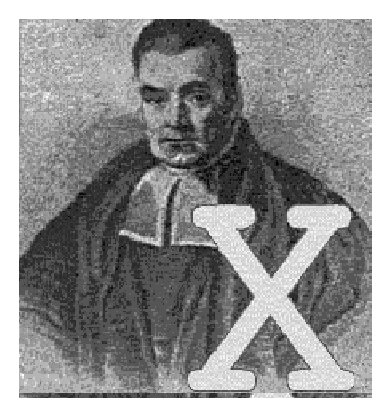
\includegraphics[scale=1.2]{grafiken/bayesicon.eps}
\end{center}
\end{figure}

\vfill

{\bf\sffamily \huge #1}

\vfill

\end{center}

{\em Developed by}

Christiane Belitz\\
Andreas Brezger\\
Nadja Klein (University of G\"{o}ttingen)\\
Thomas Kneib (University of G\"{o}ttingen)\\
Stefan Lang (University of Innsbruck) \\
Nikolaus Umlauf (University of Innsbruck) \\

\vspace{2ex}

{\em With contributions by}

\vspace{-1.5ex}

\begin{multicols}{2}
Daniel Adler\\
Paul Cochrane\\
Jan Fahrenholz\\
Eva-Maria Fronk\\
Felix Heinzl\\
Andrea Hennerfeind\\
Manuela Hummel\\
Alexander Jerak\\
Susanne Konrath\\
Petra Kragler\\
Cornelia Oberhauser\\
Leyre Est\'{\i}baliz Osuna Echavarr\'{\i}a\\
Daniel Saban\'{e}s Bov\'{e} \\
Achim Zeileis
\end{multicols}

{\em Supported by}

Ludwig Fahrmeir (mentally)\\
Leo Held (mentally)\\
German Research Foundation (DFG)

\newpage

\subsection*{Acknowledgements}

The development of {\em BayesX} has been supported by grants from the German Research Foundation (DFG), Collaborative
Research Center 386 ``Statistical Analysis of Discrete Structures''.

Special thanks go to (in alphabetical order of first names):

{\em Dieter Gollnow} for computing and providing the map of Munich (a really hard job); \\
{\em Leo Held} for advertising the program; \\
{\em Ludwig Fahrmeir} for his patience with finishing the program and for carefully
reading and correcting the  manual; \\
{\em Ngianga-Bakwin Kandala} for being the first user of the program (a really hard job); \\
{\em Samson Babatunde Adebayo} for carefully reading and correcting the manual; \\
{\em Ursula Becker} for carefully reading and correcting the manual;

\subsection*{Licensing agreement}

This program is free software; you can redistribute it and/or
modify it under the terms of the GNU General Public License
as published by the Free Software Foundation; either version 2
of the License, or (at your option) any later version.

This program is distributed in the hope that it will be useful,
but WITHOUT ANY WARRANTY; without even the implied warranty of
MERCHANTABILITY or FITNESS FOR A PARTICULAR PURPOSE.  See the
GNU General Public License for more details.

You should have received a copy of the GNU General Public License
along with this program; if not, write to the Free Software
Foundation, Inc., 51 Franklin Street, Fifth Floor, Boston, MA  02110-1301, USA.



\vspace{0.5cm}

{\em BayesX} is available at { \href{http://www.bayesx.org}{http://www.bayesx.org}}}


 \externaldocument{manual}
 \externaldocument{manual_tutorials}

 \makeindex

\begin{document}
\MakeShortVerb{\#}

\preface{Methodology Manual}

\newpage

\section{Introduction}

In this manual we provide a brief review of the methodological background for the four regression tools currently implemented
in {\em BayesX}. The first two regression tools ({\em bayesreg objects} and {\em mcmcreg objects}) rely on Markov chain Monte Carlo (MCMC) simulation
techniques and yields fully Bayesian posterior mean or posterior mode estimates. While {\em bayesreg objects} provide access to exponential family structured additive regression as well as survival times and multi-state models, {\em mcmcreg objects} implement distributional and quantile structured additive regression models as well as multilevel extensions of structure additive regression.
The third regression tool ({\em remlreg objects}) is based on the mixed model representation of penalised regression models with inference being based on penalised
maximum likelihood and marginal likelihood (a generalisation of restricted maximum likelihood) estimation. The fourth regression
tool ({\em stepwisereg objects}) simultaneously performs model choice and estimation with inference being based on penalised
likelihood. MCMC techniques are partly used for computing interval estimates. All regression tools allow to estimate structured
additive regression (STAR) models (\citeasnoun{BelLan08}, \citeasnoun{BreLan06}, \citeasnoun{FahKneLan04}) with complex semiparametric predictors.
STAR models cover a number of well
known model classes as special cases, including {\em generalized additive models} \cite{HasTib90}, {\em generalized additive
mixed models} \cite{LinZha99}, {\em geoadditive models} \cite{KamWan03}, {\em varying coefficient models} \cite{HasTib93}, and
{\em geographically weighted regression} \citeasnoun{FotBruCha02}. Besides models for responses from univariate exponential
families, BayesX also supports non-standard regression situations such as models for categorical responses with either ordered
or unordered categories, uni- and multivariate distributional regression in the spirit of generalised additive models for location, scale and shape with parametric response distributions beyond the exponential family framework, Bayesian quantile regression, continuous time survival data, or continuous time multi-state models. To provide a first impression of
structured additive regression, Sections~\ref{obsmodel} to \ref{inference} describe STAR models for exponential family
regression. Section~\ref{survivalAnalysis} extends structured additive regression to the analysis of survival times and
multi-state data while Section~\ref{distreg_star} considers extensions for distributional regression, quantile regression and multilevel specifications. Full details on STAR methodology can be found in the following references:

\subsubsection*{Structured additive regression based on MCMC
simulation}

\begin{itemize}
\item Brezger, A., Lang, S. (2006): Generalized Structured Additive Regression based on Bayesian P-Splines. {\it
    Computational Statistics and Data Analysis}, {\bf 50}, 967--991.
    \vspace{-0.25cm}
\item Brezger, A., Lang, S. (2008)
      Simultaneous Probability Statements for Bayesian P-splines.
      {\it Statistical Modelling}, {\bf 8},
      141--168.\vspace{-0.25cm}
\item Brezger, A., Steiner, W. (2008): Monotonic Regression based on Bayesian P-Splines: an Application to Estimating Price Response Functions from Store-level Scanner Data. {\it Journal of Economic and Business Statistics}, {\bf 26}, 90--104. \vspace{-0.25cm}
\item Fahrmeir, L.,  Kneib, T., Lang, S., Marx, B. (2013):
{\it Regression: Models, Methods and Applications},
 New York: Springer-Verlag.\vspace{-0.25cm}
 \item Fahrmeir, L., Lang, S. (2001): Bayesian Inference for Generalized Additive Mixed Models based on Markov Random Field
    Priors. {\it Journal of the Royal Statistical Society C (Applied Statistics)}, {\bf 50}, 201--220.\vspace{-0.25cm}
\item Fahrmeir, L., Lang, S. (2001): Bayesian Semiparametric Regression Analysis of Multicategorical Time-Space Data. {\it
    Annals of the Institute of Statistical Mathematics}, {\bf 53}, 10--30.\vspace{-0.25cm}
\item Fahrmeir, L., Osuna, L.. (2006): Structured Additive Regression for Overdispersed and Zero-Inflated Count Data. {\it
    Applied Stochastic Models in Business and Industry}, {\bf 22}, 351--369.\vspace{-0.25cm}
\item Hennerfeind, A., Brezger, A., Fahrmeir, L. (2006): Geoadditive Survival Models. {\it Journal of the American
    Statistical Association}, {\bf 101}, 1065--1075.\vspace{-0.25cm}
\item Klein, N., Kneib, T., Lang, S. (2013): Bayesian Structured Additive Distributional Regression.  Under revision for {\it Annals of Applied Statistics}.\vspace{-0.25cm}
\item Klein, N., Kneib, T., Lang, S. (2014): Bayesian Generalized Additive Models for Location, Scale and Shape for Zero-Inflated and Overdispersed Count Data. To appear in {\it Journal of the American Statistical Association}, doi:10.1080/01621459.2014.912955.\vspace{-0.25cm}
\item Klein, N., Kneib, T., Klasen, S., Lang, S.(2014): Bayesian Structured Additive Distributional Regression for Multivariate Responses. To appear in {\it Journal of the Royal Statistical Society C}, doi:10.1111/rssc.12090.\vspace{-0.25cm}
\item Kneib, T., Hennerfeind, A. (2006) Bayesian Semiparametric Multi-State Models. {\it Statistical Modelling}, {\bf 8},
    169--198..\vspace{-0.25cm}
\item Lang, S., Brezger, A. (2004): Bayesian P-Splines {\it Journal of Computational and Graphical Statistics}, {\bf 13},
    183--212.\vspace{-0.25cm}
\item Lang, S., Umlauf, N., Wechselberger, P., Harttgen, K. and Kneib, T. (2014): Multilevel Structured Additive Regression, {\it Statistics and Computing}, {\bf 24}, 223--238
\end{itemize}

Presumably the best starting point is the paper by \citeasnoun{BreLan06} or the monograph by Fahrmeir et al. (2013).

\begin{figure}[ht]
\footnotesize
\begin{center}
%\begin{tabular}{|p{8cm}|p{5cm}|}
%\hline
%{\bf Intended use} & {\bf recommended sections } \\
%\hline
%semiparametric regression, fully Bayesian approach  & sections \ref{obsmodel}, \ref{priorassumptions} , \ref{fullbayes} \\
%\hline
%semiparametric regression, inference based on mixed model technology, classical perspective &
%sections \ref{obsmodel}, \ref{penalizedleastsquares}, \ref{glmmrep}, \ref{glmmmeth} \\
%\hline
%semiparametric regression, inference based on mixed model technology, Bayesian point of view & sections \ref{obsmodel}, \ref{priorassumptions},
%\ref{glmmrep}, \ref{glmmmeth} \\
%\hline
%semiparametric regression including model choice & sections \ref{obsmodel}, \ref{penalizedleastsquares}, \ref{stepwiseest} \\
%\hline
%\end{tabular}
% \vspace{3mm}
\[\mbox{
 \beginpicture
 \setcoordinatesystem units <1.0cm,1.0cm> point at 0 0
 \setlength{\unitlength}{1.0cm}

 \put {\framebox(5.5,0.7){\sffamily\bfseries 2 Generalized regression models}} at 0 0

 \put {Bayesian perspective} at -4 -1.2
 \put {frequentist perspective} at 4 -1.2

 \arrow <4mm> [0.25,0.75] <0pt,5mm> from 0 -1 to -5 -2.9
 \arrow <4mm> [0.25,0.75] <0pt,5mm> from 0 -1 to 5 -2.9

 \put {\framebox(4.5,0.7){\sffamily\bfseries 4 Bayesian point of view}} at -5 -3

 \put {\framebox(4.5,0.7){\sffamily\bfseries 3 Penalised likelihood}} at 5 -3

 \arrow <4mm> [0.25,0.75] <0pt,5mm> from -5 -4 to 0 -6
 \arrow <4mm> [0.25,0.75] <0pt,5mm> from 5 -4 to 0 -6

 \put {relation to mixed models} at 0 -4.5

 \put {\framebox(5.5,0.7){\sffamily\bfseries 5 Mixed model representation}} at 0 -6

 \arrow <4mm> [0.25,0.75] <0pt,5mm> from -5 -4 to -5 -13
 \arrow <4mm> [0.25,0.75] <0pt,5mm> from -5 -8 to 0 -13
 \arrow <4mm> [0.25,0.75] <0pt,5mm> from 5 -4 to 5 -9

 \put {\framebox(3.5,0.7){\sffamily\bfseries 6.1 bayesreg object}} at -5 -13
 \put {\framebox(3.5,0.7){\sffamily\bfseries 6.3 stepwisereg objects}} at 5 -9

 \put {MCMC (full Bayes)} at -6.5 -6
 \put {penalised likelihood} at 6.5 -5.75
 \put {incl. model choice} at 6.4 -6.25

 \arrow <4mm> [0.25,0.75] <0pt,5mm> from 0 -7 to 0 -9

 \put {penalised likelihood} at -1.5 -7.5
 \put {(empirical Bayes)} at 1.3 -7.5

 \put {\framebox(3.5,0.7){\sffamily\bfseries 6.2 remlreg objects}} at 0 -9
 \put {\framebox(3.5,0.7){\sffamily\bfseries 8 mcmcreg objects}} at 0 -13

 \put {exponential family} at -6.4 -10
 \put {durations} at -5.8 -10.5
 \put {categorical responses} at -6.6 -11

 \put {distributional regression} at -0.6 -10
 \put {quantile regression} at -0.4 -10.5
 \put {multilevel models} at 0.1 -11

 \endpicture
}\]
 \vspace{3mm}

{\em \caption {\label{guideline} Guidelines for reading this
manual.}}
\end{center}
\end{figure}

\subsubsection*{Structured additive regression based on mixed model
methodology}

\begin{itemize}
\item Fahrmeir, L., Kneib, T., Lang, S. (2004): Penalized Structured Additive Regression for Space-Time Data: a Bayesian
    Perspective. {\it Statistica Sinica}, {\bf 14}, 715--745.\vspace{-0.25cm}
\item Kneib, T. (2006): Mixed Model based Inference in Structured Additive Regression. Dr. Hut Verlag, M\"{u}nchen. Available
    online from
    \href{http://edoc.ub.uni-muenchen.de/archive/00005011/}{http://edoc.ub.uni-muenchen.de/archive/00005011/}\vspace{-0.25cm}
\item Kneib, T. (2006): Geoadditive Hazard Regression for Interval Censored Survival Times. {\it Computational Statistics
    and Data Analysis}, {\bf 51}, 777--792.\vspace{-0.25cm}
\item Kneib, T., Fahrmeir, L. (2007): A Mixed Model Approach for Geoadditive Hazard Regression. {\it Scandinavian Journal
    of Statistics}, {\bf 34}, 207--228.\vspace{-0.25cm}
\item Kneib, T., Fahrmeir, L. (2006): Structured Additive Regression for Multicategorical Space-Time Data: A Mixed Model
    Approach. {\it Biometrics}, {\bf 62}, 109--118.\vspace{-0.25cm}
\item Kneib, T., Hennerfeind, A. (2006): Bayesian Semiparametric Multi-State Models. {\it Statistical Modelling}, {\bf 8},
    169--198.
\end{itemize}

Presumably the best starting point is the paper by \citeasnoun{FahKneLan04} or the monograph by \citeasnoun{Kne06}.

\subsubsection*{Structured additive regression including model selection}

\begin{itemize}
\item Belitz, C. (2007): Model Selection in Generalised Structured Additive Regression Models. Dr. Hut Verlag, M\"{u}nchen.
\item Belitz, C., Lang, S. (2008) Simultaneous Selection of Variables and Smoothing Parameters
in Structured Additive Regression Models. {\it
Computational Statistics and Data Analysis}, {\bf 53} , 61-81.
\end{itemize}

Presumably the best starting point is the paper by \citeasnoun{BelLan08}.

\subsubsection*{Guideline for the reader}


The rest of this manual is organized as follows:

The next section describes the general structure of STAR models for
distributions of the response variable belonging to an exponential
family. The following Sections~\ref{penalizedleastsquares} --
\ref{inference} discuss alternative approaches for specifying and
estimating the different model terms in STAR models. Section
\ref{penalizedleastsquares} describes the models from a more
classical penalized least squares perspectives. A Bayesian point of
view is taken in Section \ref{priorassumptions}. The close
connection to mixed models is highlighted in Section \ref{glmmrep}.
Section \ref{inference} gives a brief outline of the various
inference techniques for exponential family STAR models. Fully Bayesian inference via
MCMC simulation techniques for exponential family responses, categorical responses and duration times is the topic of Section \ref{fullbayes}.
Inference based on mixed model technology is sketched in Section
\ref{glmmmeth}. Simultaneous selection of relevant model terms and
estimation of the parameters is described in Section
\ref{stepwiseest}. Section~\ref{survivalAnalysis} discusses extensions for duration times and multi-state models while Section~\ref{distreg_star} provides details on distributional regression, quantile regression and multilevel specifications.

For most users of BayesX it is sufficient to read only parts of this
manual. Some recommendations are given in Figure \ref{guideline}.


\section{Generalized regression models}
\label{obsmodel}

\index{Generalized linear model}\index{Exponential family}
Generalized linear models assume that, given covariates $\uvec$ and
unknown parameters $\gammavec$, the distribution of the response
variable $y$ belongs to an exponential family, i.e.
\begin{equation}
\label{likel} p(y \, | \, \uvec) = \exp \left( \frac{y \theta -
b(\theta)}{\phi} \right) c(y,\phi)
\end{equation}
where $b(\cdot)$, $c(\cdot)$, $\theta$ and $\phi$ determine the specific response distribution. A list of the most common
distributions and their parameters can be found for example in \citeasnoun{FahTut01}, page 21. The mean
$\mu=E(y|\uvec,\gammavec)$ is linked to a linear predictor $\eta$ by
\begin{equation}
\label{glm} \mu=h(\eta) \qquad \eta= \uvec'\gammavec,
\end{equation}
where $h$ is a known response function and $\gammavec$ are unknown
regression parameters.

In most practical regression situations, however, we are facing at
least one of the following problems:
\begin{itemize}
\item For the {\em continuous covariates} in the data set, the assumption of a strictly linear
effect on the predictor may be not appropriate. \vspace{-0.2cm}
\item Observations may be {\em spatially correlated}.
\vspace{-0.2cm}
\item Observations may be {\em temporally correlated}.
\vspace{-0.2cm}
\item Complex interactions may be required to model the joint effect
of some of the covariates adequately. \vspace{-0.2cm}
\item  Heterogeneity among individuals or units may be not sufficiently described by covariates. Hence,
unobserved {\em unit or cluster specific heterogeneity} has to be
considered appropriately.
\end{itemize}
To overcome these difficulties, we replace the strictly linear
predictor in (\ref{glm}) by a structured additive predictor
\begin{equation}
\label{gampred} \eta=f_{1}(x_{1})+\ldots+f_j(x_j) +
\ldots+f_{p}(x_{p})+\uvec'\gammavec,
\end{equation}
where $x_j$ denote
covariates of different type and dimension, and $f_j$ are (not
necessarily smooth) functions of the covariates. The functions $f_j$
comprise usual nonlinear effects of continuous covariates, time
trends and seasonal effects, two-dimensional surfaces, varying
coefficient models, i.i.d. random intercepts and slopes as well as
spatial effects. STAR-models cover a number of special cases
well known from the literature, in particular {\em Generalized additive models (GAM)},
{\em Generalized additive mixed models (GAM)}, {\em Geoadditive models}, {\em Multilevel models},
{\em Varying coefficient models (VCM)}, {\em ANOVA type interaction models} and {\em geographically weighted regression}.

\section{Penalized least squares}
\label{penalizedleastsquares}

In BayesX, the nonlinear functions $f_j$ are modeled by a basis
functions approach, i.e. a particular nonlinear function $f$ is
approximated by a linear combination of basis functions:
$$
f(x) = \sum_{k=1}^{K} \beta_k B_k(x)
$$
The $B_k$ are known basis functions and $\betavec =
(\beta_1,\dots,\beta_K)'$ is a vector of unknown regression
coefficients to be estimated. Note that the term basis function in
our understanding is not limited to basis functions known from
nonparametric smoothing such as B-splines but also refers to
non-standard basis functions such as indicator functions for regions
or clusters. To ensure enough flexibility, typically a large number
of basis functions is defined. To avoid overfitting, a roughness
penalty on the regression coefficients is additionally specified. We
use quadratic penalties of the form $\betavec' \Pvec(\lambdavec)
\betavec$ where $\Pvec(\lambdavec)$ is a penalty matrix. The penalty
depends on one or multiple smoothing parameters $\lambdavec$ that
govern the amount of smoothness imposed on the function $f$. Most
penalty matrices are of the particular simple form
$\Pvec(\lambdavec) = \lambda \Kvec$ where $\lambda$ is a scalar
smoothing parameter. For {\em stepwisereg objects} more complicated
penalties are sometimes possible. They are an additive combination
of penalty matrices. An example is $\Pvec(\lambdavec) = \lambda_1
\Kvec_1+\lambda_2 \Kvec_2$ where $\lambda_1$ and $\lambda_2$ are
smoothing parameters and $\Kvec_1$ and $\Kvec_2$ are penalty
matrices.

The choice of basis functions $B_1,\dots,B_K$ and penalty  $\Pvec(\lambdavec)$ depends on our prior assumptions about the smoothness
of $f$ as well as
the type and dimension of $x$. We will give specific examples below. Defining the $n \times K$ design matrix $\Xvec$ with elements
$X[i,k] = B_k(x_i)$ the
vector $\fvec = (f(x_1),\dots,f(x_n))'$ of function evaluations can be written in matrix notation as $\fvec = \Xvec \betavec$.
Accordingly,  for model (\ref{gampred}) we obtain
$$
\etavec = \Xvec_1 \betavec_1 + \ldots + \Xvec_p \betavec_p + \Uvec \gammavec +  \varepsilonvec,
$$
where $\Uvec$ is the design matrix for linear effects, $\gammavec$ is the vector of regression coefficients for linear effects, and
$\varepsilonvec$
are the vectors of observations and errors.
In the next subsections we will give specific examples for modeling the unknown functions $f_j$ or in other words for the choice of basis functions and
penalty matrices.
We start with modeling the effect of continuous covariates using splines.

\subsection{Continuous covariates}
\subsubsection{P(enalized)-splines}
Suppose first that a particular component $x$ of the covariate  is univariate and continuous. There is a considerable amount of
literature on basis functions approaches in combination with a (quadratic) roughness penalty for continuous covariates. BayesX
applies the P-splines approach introduced by \citeasnoun{EilMar96}. The approach assumes that the unknown functions can be
approximated by a polynomial spline of degree $l$ and with equally spaced knots
$$
x_{min} = \zeta_{0}  < \zeta_{1} < \dots < \zeta_{m-1} < \zeta_{m} = x_{max}
$$
over the domain of $x$. The spline can be written in terms of a linear combination of $K=m+l$ B-spline basis functions. The
columns of the design matrix $\Xvec$ are given by the B-spline basis functions evaluated at the observations $x_i$. To overcome
the well known difficulties involved with regression splines, \citeasnoun{EilMar96} suggest a relatively large number of knots
(usually between 20 to 40) to ensure enough flexibility, and to introduce a roughness penalty on adjacent regression
coefficients based on squared $r$-th order differences, i.e.
$$
\betavec' \lambda \Kvec \betavec = \lambda \sum_{k=r+1}^K (\Delta^r \beta_k)^2.
$$
The penalty matrix is given by $\Kvec =  \Dvec_r' \Dvec_r$ where $\Dvec_r$ is a $r$-th order difference matrix.
Typically, second or third order differences are used. The limiting behavior $\lambda \rightarrow \infty$ depends both on the
order of the spline
and the order of the penalty. If the order of the spline is equal to or
higher than the order of  the penalty, which is typically the case, then a polynomial
fit of degree $r-1$ is obtained in the limit.

The approach can be extended to impose monotonicity or more general shape constraints. We follow an approach proposed by
\citeasnoun{BolEilvMe06}. A sufficient condition for a decreasing spline is given by $\beta_{k} \leq \beta_{k-1}$, i.e.  a
parameter $\beta_{k}$ is less than its predecessor $\beta_{k-1}$. The simple but powerful idea  is to impose the required
constraint by expanding the penalty by an additional  term. More specifically they propose the composed penalty
$$
\Pvec(\lambdavec) =  \betavec' \left( \lambda_1 \Kvec_1 + \lambda_2 \Kvec_2 \right) \betavec
$$
where $\lambda_1$ and $\Kvec_1$ are the usual smoothing parameter
and penalty matrix for P-splines. The additional penalty matrix
$\Kvec_2$ is a diagonal matrix with entries 1 whenever the condition
$\beta_{k} \leq \beta_{k-1}$ fails and 0 otherwise. For increasing
functions, $\Kvec_2$ has to be adapted accordingly. The parameter
$\lambda_2$ is not estimated but set large enough to enforce
monotonic functions.





\subsubsection{Tensor product P-splines}
\label{tensorproductpsplines} Assume now that $\xvec$ is
two-dimensional, i.e. $\xvec = \left(x^{(1)},x^{(2)}\right)'$ with
continuous components $x^{(1)}$ and $x^{(2)}$. The aim is to extend
the univariate P-spline from the preceding section to two
dimensions. A common approach is to approximate the unknown surface
$f(x)$ by the tensor product of one dimensional B-splines, i.e.
\begin{equation}
\label{gampspline_2dimterm} f\left(x^{(1)},x^{(2)}\right) = \sum_{k=1}^{K_1}
\sum_{s=1}^{K_2} \beta_{ks} B_{1,k}(x^{(1)})
B_{2,s} (x^{(2)}),
\end{equation}
where $B_{11},\dots,B_{1K_1}$ are the basis functions in $x^{(1)}$ direction and
$B_{21},\dots,B_{2K_2}$ in $x^{(2)}$ direction.
The $n \times K = n \times K_1 K_2$ design matrix $\Xvec$ now consists of
products of basis functions.

Several alternatives are available for the penalty matrix $\Pvec(\lambdavec)$:
\begin{enumerate}
\item[a)] {\em Penalty based on first differences:} The
two-dimensional generalization of a penalty based on first
differences is given by combining row- and column wise quadratic
differences
$$
\begin{array}{l}
\displaystyle \sum_{k=2}^{K_1}\sum_{s=1}^{K_2}(\beta_{ks}-\beta_{k-1,s})^2 =
\betavec'(\Ivec_{K_2}\otimes \Dvec_1)'(\Ivec_{K_2}\otimes \Dvec_1)\betavec \\[0.4cm]
\displaystyle  \sum_{k=1}^{K_1}\sum_{s=2}^{K_2}(\beta_{ks}-\beta_{k,s-1})^2 =
\betavec'(\Dvec_2\otimes \Ivec_{K_1})'(\Dvec_2\otimes \Ivec_{K_1})\betavec \\
\end{array}
$$
to the penalty
$$
\betavec'\Pvec(\lambdavec) \betavec =  \betavec' \lambda \left[ (\Ivec_{K_2}\otimes \Dvec_1)'(\Ivec_{K_2}\otimes \Dvec_1) + (\Dvec_2\otimes \Ivec_{K_1})'
(\Dvec_2\otimes \Ivec_{K_1})\right]\betavec.
$$
Another way of expressing the penalty is given by
\begin{equation}
\label{2dpenalty}
 \betavec'\Pvec(\lambda)\betavec = \betavec'\lambda \left[\Ivec_{K_2}\otimes\Kvec_1 + \Kvec_2\otimes \Ivec_{K_1}\right]\betavec,
\end{equation}
where $\Kvec_1$ and $\Kvec_2$ are the respective one dimensional penalty matrices.
In the limit  $\lambda \rightarrow \infty$ a constant fit is obtained.
\item[b)] {\em Penalty based on second differences:} In a similar way two-dimensional penalties based on higher order differences
are constructed. A second order difference penalty is obtained if
$\Kvec_1$ and $\Kvec_2$ in (\ref{2dpenalty}) correspond to penalty
matrices based on second rather than first differences. Similar to
one dimensional P-splines the limit $\lambda \rightarrow \infty$
results in linear effects in $x^{(1)}$ and $x^{(2)}$ with an
additional interaction effect, i.e.
$$
f\left(z^{(1)},z^{(2)}\right) = c_0 + c_1 \, x^{(1)} + c_2 \,
x^{(2)} + c_3 \, x^{(1)} x^{(2)}.
$$
\item[c)] {\em Anisotropic penalty:} The two penalties considered so far are not capable of
different penalization in $x^{(1)}$ and $x^{(2)}$ direction,
respectively. Anisotropic penalties are obtained by assuming
separate smoothing parameters $\lambda_1$ and $\lambda_2$ in
$x^{(1)}$ and $x^{(2)}$ direction. The penalty is then given by
\begin{equation}
\label{penalty_eilmar}
 \betavec'\Pvec(\lambdavec) \betavec = \betavec'\left[\lambda_1 \Ivec_{K_2}\otimes\Kvec_1 + \lambda_2 \Kvec_2\otimes \Ivec_{K_1}\right]\betavec.
\end{equation}
The resulting fit in the limit $\lambda_1 \rightarrow \infty$ and
$\lambda_2 \rightarrow \infty$ depends on the penalty used to
construct $\Kvec_1$ and $\Kvec_2$. If $\Kvec_1$ and $\Kvec_2$
correspond to a first order difference penalty a constant fit is
obtained in the limit. Second order difference penalties result in a
linear fit for $f\left(x^{(1)},x^{(2)}\right)$.
\item[d)] {\em Penalties with main effects in the limit:} Sometimes it is desirable to decompose the effect of the two covariates
$x^{(1)}$ and $x^{(2)}$ into two main effects modeled by one
dimensional functions and a two-dimensional interaction effect, i.e.
\begin{equation}
\label{pspline_2dimtermmain} f \left(x^{(1)},x^{(2)}\right) =
f_1\left(x^{(1)} \right) + f_2 \left(x^{(2)}\right) + f_{1|2}\left(
x^{(1)},x^{(2)} \right).
\end{equation}
Usually a two-dimensional surface smoother  together with two
additional  one dimensional P-splines (or other smoothers) are
estimated. This approach is possible with {\em bayesreg objects} and
{\em remlreg objects}. {\em stepwisereg objects} take, however, a
different approach. We specify a two-dimensional surface based on
tensor product P-splines and compute the decomposition of the
resulting surface into main effects and the interaction effect {\em
after} estimation. Moreover, we specify a penalty that allows for a
main effects only model as a special case. This allows to
discriminate between a simple  main effects model and a more
complicated two way interactions model. A penalty that guarantees  a
main effects model in the limit is defined by the Kronecker product
of the two penalty matrices for one dimensional P-splines, i.e.
\begin{equation}
\label{penalty_kronecker}
\betavec'\Pvec(\lambda)\betavec = \betavec' \lambda \Kvec_1 \otimes \Kvec_2 \betavec.
\end{equation}
The drawback of this penalty is that the limit $\lambda \rightarrow \infty $ yields {\em unpenalized} main effects, i.e. wiggly functions.
We therefore use a modified penalty which is effectively a combination of the two  penalties  (\ref{penalty_eilmar}) and
(\ref{penalty_kronecker}). More specifically
we define
\begin{equation}
\label{penalty_comb}
\betavec'\Pvec(\lambdavec)\betavec = \betavec' \left[\frac{\lambda_1}{K_1}
\Ivec_{K_2}\otimes\Kvec_1 + \frac{\lambda_2}{K_2} \Kvec_2\otimes \Ivec_{K_1}+\lambda_3 \Kvec_1 \otimes \Kvec_2   \right] \betavec,
\end{equation}
where $\Kvec_1$ and $\Kvec_2$ are penalty matrices corresponding to one dimensional P-splines based on first or second order differences.
This penalty has the following nice properties:
\begin{itemize}
\item The limit $\lambda_3 \rightarrow \infty$ results in a mere main effects model. The main effects  are one dimensional P-splines with smoothing
parameters $\lambda_1$ and $\lambda_2$.
\item The limit $\lambda_3 \rightarrow 0$ yields the anisotropic penalty (\ref{penalty_eilmar}) as a special case.
\item The limit $\lambda_1 \rightarrow 0$ and $\lambda_2 \rightarrow 0$  yields the Kronecker product penalty
(\ref{penalty_kronecker}) as a special case.
\item The limit $\lambda_1 \rightarrow \infty$, $\lambda_2 \rightarrow \infty$ and $\lambda_3 \rightarrow \infty$ results in a main effects model with
linear or constant main effects depending on the difference order used to construct $\Kvec_1$ and $\Kvec_2$.
\end{itemize}
\end{enumerate}


\subsection{Spatial effects}

In this subsection we assume that $x$ represents the location a
particular observation pertains to. The location is typically given
in two ways. If exact locations are available $x=(x^{(1)},x^{(2)})'$
is two-dimensional and the components  $x^{(1)}$ and $x^{(2)}$
correspond to the coordinates of the location. In this case, the
spatial effect $f(x^{(1)},x^{(2)})$ could be modeled by
two-dimensional surface estimators as described in the preceding
section.

In many applications, however, exact locations are not available. Typically, a geographical map is available and $x \in \{1,\dots,K\}$ is an
index that denotes the region (e.g. district) an observation pertains to. A common approach is to assume $f(x) = \beta_x$,
i.e. separate parameters $\beta_1,\ldots,\beta_K$  for each region are estimated.
The $n \times K$ design matrix $\Xvec$ is an incidence matrix whose entry in
the $i$-th row and $k$-th column is equal to one if observation $i$ has been observed at
location $k$ and zero otherwise. To prevent overfitting a penalty based on squared differences is defined that
guarantees that parameters of neighboring regions are similar. Typically two regions are assumed to be neighbors if they share a common
boundary although other neighborhood definitions are possible. The penalty is defined as
$$
\betavec' \lambda \Kvec \betavec = \lambda\sum_{k=2}^{K}\sum_{s \in N(k), s < k}(\beta_k-\beta_s)^2,
$$
where $N(k)$ denotes all sites that are neighbors of site $k$.
The elements of the penalty matrix are given by
\begin{equation}
\label{K_mrf}
 \Kvec[s,r] = \lambda \left\{
 \begin{array}{ll}
-1 & k\neq s, k\sim s,\\
 0 & k\neq s, k \nsim s,\\
 |N(k)| & k=s.
\end{array}
\right.
\end{equation}

Depending on the prior belief on smoothness of the spatial effect
several alternatives to penalty (\ref{K_mrf}) are available. If a
very smooth effect is assumed, the two-dimensional smoothers
discussed in the preceding section could be used as an alternative.
Since exact locations are not available the centroids of the regions
could be used instead.

\subsection{Unit- or cluster specific heterogeneity}
Typically, unit- or cluster specific random effects are introduced
to account for unobserved heterogeneity. In its simplest form, a
random intercept $\beta_x$ with $\beta_x \sim N(0,\tau^2)$ is
introduced. Here, $x \in \{1,\dots,K\}$ is an index variable that
denotes the cluster a particular observation pertains to. This is
equivalent to a penalized least squares approach with function $f(x)
= \beta_x$, penalty matrix $\Ivec$ and smoothing parameter $\lambda
= \sigma^2/\tau^2$. The $n \times K$ design matrix $\Xvec$ is a 0/1
incidence matrix whose entry in the $i$-th row and $k$-th column is
equal to one if observation $i$ belongs to the $k$-th cluster and
zero otherwise. Random slopes could be treated in the same way, see
the next subsection.

A particular cluster variable is a spatial index that indicates the region an observation pertains to. Usually a spatially correlated effect
as described in the preceding subsection is specified.
However, in some situations a smooth spatial effect is not justified because of local, spatial heterogeneity. In this case,
the assumption of spatial dependence of neighboring parameters is not meaningful. Instead, the simple (ridge type) penalty
$$
\betavec' \lambda \Kvec \betavec = \lambda \betavec'  \betavec = \lambda \sum_{k=1}^{K} \beta_k^2
$$
with penalty matrix $\Kvec = \Ivec$ may be defined. This penalty does not assume any spatial dependence but prevents highly variable
estimates induced by small samples for some regions or sites.

Note that more than one random intercept with respect to different
cluster variables are possible. In many cases there exists a
hierarchical ordering of clusters. Models with such hierarchical
clusters are also called multilevel models.


\subsection{Varying coefficients}
\label{varcoeff_terms}

Suppose now that the effect of a continuous covariate $x^{(2)}$ is assumed to vary with
respect to a categorical covariate $x^{(1)}$. For notational convenience, we restrict the discussion to binary covariates $x^{(1)}$.
The generalization to (multi)categorical covariates is straightforward.
The interaction between $x^{(2)}$ and
$x^{(1)}$ can be modeled by a predictor of the form
$$
\eta = \ldots + f_1(x^{(2)}) + g(x^{(2)}) x^{(1)} + \ldots,
$$
where $f_1$ and $g$ are smooth functions (modeled by P-splines). The
interpretation of the two functions $f_1$ and $g$ depends on the
coding of the binary variable $x^{(1)}$. If $x^{(1)}$ is in
dummy-coding, the function $f_1$ corresponds to the effect of
$x^{(2)}$ subject to  $x^{(1)}=0$, and $g$ is the difference effect
for observations with $x^{(1)}=1$. If $x^{(1)}$ is in effect-coding,
the function $f_1$ can be interpreted as an average effect of
$x^{(2)}$, where $g$ and $-g$ represent the deviation from $f_1$ for
$x^{(1)} = 1$ and $x^{(1)} = -1$, respectively. It turns out that
the coding of $x^{(2)}$ is not only important  for interpretation
but sometimes also crucial for inference (in {\em bayesreg objects}
and {\em stepwisereg objects}). Estimation for {\em bayesreg and
stepwisereg objects} described in the next section is based on an
iterative backfitting type procedure. Hence dependence between $f_1$
and $g$ should be minimized to avoid convergence problems. Hence,
effect coding for $x^{(2)}$ is an effective yet simple device to
avoid convergence problems.

Models with interaction effects of the form $g(x^{(2)}) \, x^{(1)}$ are  known as varying coefficient models  because the
effect of $x^{(1)}$ varies smoothly with respect to the continuous covariate $x^{(2)}$. Covariate $x^{(2)}$ is called the
effect modifier of $x^{(1)}$. The approach can be easily extended to a two-dimensional effect modifier with components
$x^{(2)}$ and $x^{(3)}$. The interaction effect is then given by $g(x^{(2)},x^{(3)}) \, x^{(1)}$ where $g(x^{(2)},x^{(3)})$ is
a two-dimensional surface which is modeled by the tensor product P-splines discussed in section \ref{tensorproductpsplines}.
Another modification arises if the effect modifier is the location either given as the coordinates or as a spatial index. In
this case we have a space varying effect of $x^{(1)}$. Models of this kind are also known as geographically weighted
regression, see \citeasnoun{FotBruCha02}. A final modification is obtained for a unit or cluster index as effect modifier. The
effect of $x^{(1)}$ is now assumed to be unit- or cluster-specific and typically referred to as a random slope.

Independent of the specific type of the effect modifier, the interaction term $g\left(x^{(2)}\right) \, x^{(1)}$
(or $g\left(x^{(2)},x^{(3)}\right) \, x^{(1)}$) can be cast into our
general framework by defining
\begin{equation}
\label{gampspline_varcoeffterm}
f\left(x^{(1)},x^{(2)}\right) = g\left(x^{(2)}\right) \, x^{(1)} \quad \mbox{or} \quad  f\left(x^{(1)},x^{(2)},x^{(3)}\right) =
g\left(x^{(2)},x^{(3)}\right) \, x^{(1)}.
\end{equation}
The overall design matrix $\Xvec$ is given by
$\diag(x_{1}^{(1)},\dots,x_{n}^{(1)}) \, \Xvec^{(1)}$ where
$\Xvec^{(1)}$ is the usual design matrix for P-Splines, tensor
product P-splines, spatial-, or cluster-specific effects.



\section{Bayesian point of view}
\label{priorassumptions}\index{Prior assumptions}

For Bayesian inference, the unknown functions $f_{1},\dots ,f_{p}$
in predictor (\ref{gampred}), more exactly corresponding vectors of
function evaluations, and the fixed effects parameters $\gammavec$ are
considered as random variables and must be supplemented by
appropriate prior assumptions.

In the absence of any prior knowledge, diffuse priors are the
appropriate choice for fixed effects parameters, i.e.
$$
 p(\gamma_j) \propto const
$$
Another common choice, not yet supported by {\em BayesX}, are
informative multivariate Gaussian priors with mean $\muvec_0$ and
covariance matrix $\Sigmavec_0$.\index{Prior assumptions!Fixed effects}


Priors for the unknown functions $f_{1},\dots,f_{p}$ depend on the
{\em type of the covariates} and on {\em prior beliefs about the
smoothness of $f_j$.} In the following we express the vector of
function evaluations $\fvec_j=(f_j(x_{1j}),\dots,f_j(x_{nj}))'$ of a
function $f_j$ as the matrix product of a design matrix $\Xvec_j$ and a
vector of unknown parameters $\betavec_j$, i.e.
\begin{equation}
\label{matproduct} \fvec_j=\Xvec_j \betavec_j.
\end{equation}
Then, we obtain the predictor (\ref{gampred}) in matrix notation
as
\begin{equation}
\label{gampredmatrix} \etavec = \Xvec_1 \betavec_1 + \cdots + \Xvec_p \betavec_p +
\Uvec \gammavec,
\end{equation}
where $\Uvec$ corresponds to the usual design matrix for fixed
effects.

A prior for a function $f_j$ is defined by specifying a suitable
design matrix $\Xvec_j$ and a prior distribution for the vector
$\betavec_j$ of unknown parameters. The general form of the prior for
$\betavec_j$ is given by
\begin{equation}
\label{genform} p(\betavec_j | \tau_j^2) \propto
\frac{1}{(\tau^2_j)^{rank(\Kvec_j)/2}} \exp\left(-\frac{1}{2\tau_j^2}
\betavec_j' \Kvec_j \betavec_j\right),
\end{equation}
where $\Kvec_j$ is a {\em penalty matrix}. In most cases $\Kvec_j$ will be
rank deficient and therefore the prior for $\betavec_j$ is partially improper.

The variance parameter $\tau_j^2$ is  equivalent to the inverse
smoothing parameter in a penalized likelihood approach and controls the
trade off between flexibility and smoothness.

In the following we will describe specific priors for different
types of covariates and functions $f_j$.


\subsection{Continuous covariates}
\label{psplines}\index{Continuous covariates}\index{Time scales}
\index{Prior assumptions!Continuous covariates}

Several alternatives have been  proposed for specifying smoothness priors for continuous covariates or time scales. These are
{\em random walk priors} or more generally {\em autoregressive priors} (see \citeasnoun{FahLan01a} and \citeasnoun{FahLan01b},
{\em Bayesian P-splines} \cite{LanBre04} and {\em Bayesian smoothing splines} \cite{HasTib00}. {\em BayesX} supports random
walk priors and P-splines.

\subsubsection{Random walks}\index{Random walk priors}

Suppose first that $x$ is a time scale or continuous covariate
with equally spaced ordered observations
$$
x^{(1)} < x^{(2)} < \cdots < x^{(K)}.
$$
Here $K \leq n$ denotes the number of {\em different} observed
values for $x$ in the data set. A common approach in dynamic or
state space models is to estimate one parameter $\beta_{k}$ for
each distinct $x^{(k)}$, i.e. $f(x^{(k)}) = \beta_{k}$, and
penalize too abrupt jumps between successive parameters using random
walk priors. For example, first and second order random walk models
are given by
\begin{equation}
\label{rwpriors}
\beta_{k}=\beta_{k-1}+u_{k}\,\,\,\,\mbox{and}\,\,\,\,\beta_{k}=2\beta_{k-1}-\beta_{k-2}+u_{k}
\end{equation}
with Gaussian errors $u_{k}\sim N(0,\tau^{2})$ and diffuse priors
$p(\beta_{1})\propto const$, and $p(\beta_{1})$ and
$p(\beta_{2})\propto const$, for initial values, respectively. Both
specifications act as smoothness priors that penalize too rough
functions $f$. A first order random walk penalizes abrupt jumps
$\beta_{k}-\beta_{k-1}$ between successive states while a second
order random walk penalizes deviations from the linear trend $2
\beta_{k-1}-\beta_{k-2}$. The joint distribution of the
regression parameters $\betavec$ is easily computed as the product of
conditional densities defined by (\ref{rwpriors}) and can be brought
into the general form (\ref{genform}). The penalty matrix is of the
form $\Kvec=\Dvec'\Dvec$ where $\Dvec$ is a first or second order difference
matrix. For example, for a random walk of first order the penalty
matrix is given by:
$$
\Kvec = {\footnotesize \left(
\begin{array}{rrrrr}
 1 & -1 & & &  \\
-1 & 2 & -1 & & \\
 &  \ddots & \ddots & \ddots &  \\
 & & -1 & 2 & -1 \\
  & & & -1 & 1
\end{array}
\right) }.
$$
The design matrix $\Xvec$ is a simple 0/1 matrix where the number of
columns equals the number of parameters, i.e. the number of distinct
covariate values. If for the $i$-th observation $x_{i}=x^{(k)}$
the element in the $i$-th row and $k$-th column of $\Xvec$ is one and
zero otherwise.

In case of non-equally spaced observations slight modifications of the priors defined in (\ref{rwpriors}) are necessary, see
\citeasnoun{FahLan01a} for details.

\subsubsection{P-splines}\index{P-splines}

A second approach for effects of continuous covariates, that is closely related to random walk models, is based on P-splines
introduced by \citeasnoun{EilMar96}. The approach assumes that an unknown smooth function $f$ of a covariate $x$ can be
approximated by a polynomial spline of degree $l$ defined by a set of equally spaced knots $x_{min} = \zeta_{0}  < \zeta_{1} <
\dots < \zeta_{m-1} < \zeta_{m} = x_{max}$ within the domain of $x$. Such a spline can be written in terms of a linear
combination of $K = m+l$ B-spline basis functions $B_{k}$, i.e.
$$
f(x) = \sum_{k=1}^{K} \beta_{k} B_{k}(x).
$$
In this case, $\betavec = (\beta_{1},\dots,\beta_{K})'$ corresponds to the vector of unknown regression coefficients and the $n
\times K$ design matrix $\Xvec$ consists of the basis functions evaluated at the observations $x_{i}$, i.e. $\Xvec[i,k] =
B_k(x_{i})$. The crucial point is the choice of the number of knots. For a small number of knots, the resulting spline may not
be flexible enough to capture the variability of the data. For a large number of knots, estimated curves tend to overfit the
data and, as a result, too rough functions are obtained. As a remedy, \citeasnoun{EilMar96} suggest a moderately large number
of equally spaced knots (usually between 20 and 40) to ensure enough flexibility, and to define a roughness penalty based on
first or second order differences of adjacent B-Spline coefficients to guarantee sufficient smoothness of the fitted curves.
This leads to penalized likelihood estimation with penalty terms
\begin{equation}
\label{diffpenalty} \lambda \sum_{k=r+1}^{K}
(\Delta^r \beta_{k})^2 , \quad r=1,2
\end{equation}
where $\lambda$ is the smoothing parameter. First order differences penalize abrupt jumps $\beta_{k}-\beta_{k-1}$ between
successive parameters while second order differences penalize deviations from the linear trend $2 \beta_{k-1}-\beta_{k-2}$. In
a Bayesian approach we use the stochastic analogue of difference penalties, i.e. first or second order random walks, as priors
for the regression coefficients. Note that simple first or second order random walks can be regarded as P-splines of degree
$l=0$ and are therefore included as a special case. More details about Bayesian P-splines can be found in \citeasnoun{LanBre04}
and \citeasnoun{BreLan06}.

\subsubsection{Tensor product P-splines}
\label{tensorproductpsplines_bayes}

Assume now that $x$ is two-dimensional, i.e. $x = \left(x^{(1)},x^{(2)}\right)'$ with continuous components $x^{(1)}$ and
$x^{(2)}$. Similar to section \ref{tensorproductpsplines} the aim is to extend the univariate P-spline to two dimensions. In
{\em BayesX} Bayesian surface fitting is based on two-dimensional P-splines described in more detail in \citeasnoun{LanBre04}
and \citeasnoun{BreLan06}. The unknown surface $f(x^{(1)},x^{(2)})$ is approximated by the tensor product of two
one-dimensional B-splines, i.e.
$$
f\left(x^{(1)},x^{(2)}\right) = \sum_{k=1}^{K_1}
\sum_{s=1}^{K_2} \beta_{ks} B_{1,k}(x^{(1)})
B_{2,s} (x^{(2)}),
$$
where $B_{11},\dots,B_{1K_1}$ are the basis functions in $x^{(1)}$ direction and
$B_{21},\dots,B_{2K_2}$ in $x^{(2)}$ direction.
The $n \times K = n \times K_1 K_2$ design matrix $\Xvec$ now consists of
products of basis functions.

Priors for
$\betavec = (\beta_{11},\dots,\beta_{K_1,K_2})'$ can be based on
spatial smoothness priors common in spatial statistics, e.g.
two-dimensional first order random walks. The most commonly used
prior specification based on the four nearest neighbors is defined
by
\begin{equation}
\label{2dimrw1} \beta_{ks} | \cdot \sim N \left(
\frac{1}{4} ( \beta_{k-1,s}+ \beta_{k+1,s} +
\beta_{k,s-1} +\beta_{k,s+1}),\frac{\tau^2}{4}
\right)
\end{equation}
and appropriate edge corrections. This
prior as well as higher order bivariate random walks can be easily
brought into the general form (\ref{genform}).


\subsection{Spatial effects}\index{Spatial
priors}\index{Markov random fields}\index{Kriging}\index{Gaussian
random fields} \label{spatial}\index{Prior assumptions!Spatial
effects}

\subsubsection{Markov random fields}

Suppose that the index $s \in \{ 1,\dots,S \}$ represents the
location or site in connected geographical regions. For simplicity
we assume that the regions are labelled consecutively. A common way
to introduce a spatially correlated effect is to assume that
neighboring sites are more alike than arbitrary sites. Thus, for a
valid prior definition a set of neighbors for each site $s$ must be
defined. For geographical data one usually assumes that two sites
$s$ and $s'$ are neighbors if they share a common boundary.

The simplest (but most frequently used) spatial smoothness prior for
the function evaluations $f(s)=\beta_{s}$ is given by
\begin{equation}
\label{adjacency} \beta_{s} | \beta_{s'}, \, {s \neq
s'},\tau^2 \sim N \left( \frac{1}{N_s} \sum_{s' \in \partial_s}
\beta_{s'} , \frac{\tau^2}{N_s} \right),
\end{equation}
where $N_s$ is the number of adjacent sites and $s' \in
\partial_s$ denotes that site $s'$ is a neighbor of site $s$. Hence,
the (conditional) mean of $\beta_{s}$ is an unweighted average of
function evaluations of neighboring sites. The prior is a direct
generalization of a first order random walk to two-dimensions and is
called a Markov random field (MRF).

The $n \times S$ design matrix $\Xvec$ is a 0/1 incidence matrix. Its
value in the $i$-th row and the $s$-th column is 1 if the $i$-th
observation is located in site or region $s$, and zero otherwise.
The $S \times S$ penalty matrix $\Kvec$ has the form of an adjacency
matrix.

\subsubsection{Kriging}

If exact locations $\svec=(s_x,s_y)$ are available, we can use two-dimensional surface estimators to model spatial effects. One
option are two-dimensional P-splines, described in \autoref{tensorproductpsplines}. Another option are Gaussian random field
(GRF) priors, originating from geostatistics. These can also be interpreted as two-dimensional surface smoothers based on
radial basis functions and have been employed by \citeasnoun{KamWan03} to model the spatial component in Gaussian regression
models. The spatial component $f(\svec)=\beta_\svec$ is assumed to follow a zero mean stationary Gaussian random field
$\{\beta_\svec:\svec\in\mathbb{R}^2\}$ with variance $\tau^2$ and isotropic correlation function
$\Cov(\beta_\svec,\beta_{\svec+\hvec})=C(||\hvec||)$. This means that correlations between sites that are $||\hvec||$ units
apart are the same, regardless of direction and the sites location. For a finite array $\svec\in\{\svec_1,\ldots,\svec_S\}$ of
sites as in image analysis, the prior for $\betavec=(\beta_1,\ldots,\beta_S)'$ is of the general form (\ref{genform}) with
$\Kvec=\Cvec^{-1}$ and
\[\Cvec(i,j)=C(||\svec_i-\svec_j||), 1\le i,j\le S.\]
The design matrix $X$ is again a 0/1 incidence matrix.

Several proposals for the choice of the correlation function
$C(r)$ have been made. In the kriging literature, the Mat\'{e}rn
family $C(r;\rho,\nu)$ is highly recommended. For prechosen values $\nu=m+1/2$,
$m=0,1,2,\ldots$ of the smoothness parameter $\nu$ simple
correlation functions $C(r;\rho)$ are obtained, e.g.
\[C(r;\rho)=\exp(-|r/\rho|)(1+|r/\rho|)\]
with $\nu=1.5$. The parameter $\rho$ controls how fast correlations
die out with increasing $r=||h||$. It can be determined in a
preprocessing step or may be estimated jointly with the variance
components by restricted maximum likelihood. A simple rule, that
also ensures scale invariance of the estimates, is to choose $\rho$
as
\[\hat{\rho}=\max_{i,j}||\svec_i-\svec_j||/c.\]
The constant $c>0$ is chosen in such a way, that $C(c)$ is small,
e.g. 0.001. Therefore the different values of
$||\svec_i-\svec_j||/\hat{\rho}$ are spread out over the $r$-axis of
the correlation function. This choice of $\rho$ has proved to work
well in our experience.

\subsubsection{Discrete vs. continuous spatial smoothing}

Although we described them separately, approaches for exact locations can also be used in the case of connected geographical
regions, e.g. based on the centroids of the regions. Conversely, we can also apply MRFs to exact locations if neighborhoods are
defined based on a distance measure. In general, it is not clear which of the different approaches leads to the ''best'' fits.
For data observed on a discrete lattice MRFs seem to be most appropriate. If the exact locations are available, surface
estimators may be more natural, particularly because predictions for unobserved locations are available. However, in some
situations surface estimators lead to an improved fit compared to MRF's even for discrete lattices and vice versa. A general
approach that can handle both situations is given by \citeasnoun{MueStaTab97}.

From a computational point of view MRF's and P-splines are preferable to GRF's because their posterior precision matrices are
band matrices or can be transformed into a band matrix like structure. This special structure considerably speeds up
computations, at least for inference based on MCMC techniques. For inference based on mixed models, the main difference between
GRFs and MRFs, considering their numerical properties, is the dimension of the penalty matrix. For MRFs the dimension of $K$
equals the number of different regions $S$ and is therefore independent from the sample size. On the other side, for GRFs, the
dimension of $K$ is given by the number of distinct locations, which is usually close to the sample size. Therefore, the number
of regression coefficients used to describe a MRF is usually much smaller than for a GRF and therefore the estimation of GRFs
is computationally much more expensive. To overcome this difficulty \citeasnoun{KamWan03} propose low-rank kriging to
approximate stationary Gaussian random fields. Note first, that we can define GRFs equivalently based on a design matrix
$\Xvec$ with entries $\Xvec[i,j]=C(||\svec_i-\svec_j||)$ and penalty matrix $\Kvec=\Cvec$. To reduce the dimensionality of the
estimation problem we define a subset of knots $\mathcal{D}=\{\kappavec_1,\ldots,\kappavec_M\}$ of the set of distinct
locations $\mathcal{C}$. These knots can be chosen to be ''representative'' for the set of distinct locations $\mathcal{C}$
based on a space filling algorithm. Therefore consider the distance measure
\[d(\svec,\mathcal{D})=\left(\sum_{\kappavec\in\mathcal{D}}||\svec-\kappavec||^p\right)^{\frac{1}{p}},\]
with $p<0$, between any location $\svec\in\mathcal{D}$ and a
possible set of knots $\mathcal{C}$. Obviously this distance measure
is zero for all knots. Using a simple swapping algorithm to minimize
the overall coverage criterion
\[\left(\sum_{\svec\in\mathcal{C}}d(\svec,\mathcal{D})^q\right)^{\frac{1}{q}}\]
with $q>0$ (compare \citeasnoun{JohMooYlv90} and \citeasnoun{NycSal98} for details) yields an optimal set of knots
$\mathcal{D}$. Based on these knots we define the approximation $\fvec=\Xvec\betavec$ with the $n\times M$ design matrix
$\Xvec[i,j]=C(||\svec_i-\kappavec_j||)$, penalty matrix $\Kvec=\Cvec$, and $\Cvec[i,j]=C(||\kappavec_i-\kappavec_j||)$. The
number of knots $M$ allows to control the trade-off between accuracy of the approximation ($M$ close to the sample size) and
numerical simplification ($M$ small).

\subsection{Unit- or cluster-specific heterogeneity}
\label{random}\index{Random effects}\index{Group
indicators}\index{Unstructured spatial effects}

In many situations we observe the problem of heterogeneity among
clusters of observations caused by unobserved covariates. Neglecting
unobserved heterogeneity may lead to considerably biased estimates
for the remaining effects as well as false standard error estimates.
Suppose now $x \in \{1,\dots,K\}$ is a cluster variable indicating the
cluster a particular observation belongs to. A common approach to
overcome the difficulties of unobserved heterogeneity is to
introduce additional Gaussian i.i.d. effects $f(x) = \beta_{x}$
with
\begin{equation}
\label{randomeff} \beta_{x} \sim N(0,\tau^2), \quad
x=1,\dots,K.
\end{equation}
The design matrix $\Xvec$ is again a $n \times K$-dimensional 0/1
incidence matrix that represents the grouping structure of the data,
while the penalty matrix is simply the identity matrix, i.e.
$\Kvec=\Ivec$. From a classical perspective, (\ref{randomeff}) defines
i.i.d. {\em random effects}. However, from a Bayesian point of view
all unknown parameters are assumed to be random and hence the
notation "random effects" in this context is misleading. Hence, one
may also think of (\ref{randomeff}) as an approach for modelling an
unsmooth function.

Prior (\ref{randomeff}) may also be used for a more sophisticated
modelling of spatial effects. In some situation it may be useful to
split up the spatial effect $f_{spat}$ into a spatially correlated
(structured) part $f_{str}$ and a spatially uncorrelated
(unstructured) part $f_{unstr}$, i.e.
$$
f_{spat} = f_{str}+f_{unstr}.
$$
A rationale is that a spatial effect is usually a surrogate of many unobserved influential factors, some of which obeying a
strong spatial structure while others are present only locally. By estimating a structured and an unstructured component we aim
at distinguishing between the two kinds of influential factors, see also \citeasnoun{BesYorMol91}. For the smooth spatial part
we can assume any of the spatial priors discussed in \autoref{spatial}. For the uncorrelated part we may assume prior
(\ref{randomeff}).

\subsection{Varying coefficients}
\index{Varying coefficient models}

The models considered so far are not appropriate for modelling interactions between covariates. A common approach is based on
varying coefficient models introduced by \citeasnoun{HasTib93} in the context of smoothing splines. Varying coefficient terms
have already been discussed in the previous chapter, see section \ref{varcoeff_terms}.


\subsection{Regularization Priors for highdimensional covariates}
\label{Regularization Priors for highdimensional covariates}
\index{Regularization Priors for highdimensional covariates}

In this section the vector $\betavec _{s} =\left(\beta _{p+1} ,\ldots\beta _{p+q} \right)$ is a subvector of the unknown regression
coefficients $\gammavec$ for fixed (linear) effects. A desirable feature for variable selection is to shrink small effects to
zero but to shrink important effects only moderately to prevent them from large bias. At the opposite to the unregularized
regression coefficients where flat priors $p \left(\gammavec \right)\propto 1$ are assumed, we need informative priors
appropriate for shrinkage. Several alternatives have been proposed for specifying shrinkage priors for the regression
coefficients, see e.g. Griffin and Brown (2005). Three shrinkage priors, which are hierarchically represented as scale mixtures
of normals, are implemented in {\em BayesX}: the {\em ridge}-, the {\em lasso}- and the {\em Normal Mixture of Inverse
Gamma (NMIG)-prior}. Common for all approaches is an informative, zero mean conditional Gaussian distribution of the regression
coefficients
\[\beta _{j} |\sigma^2,\tau _{j}^{2} \mathop{\sim }\limits^{i.i.d.} N\left(0,\sigma^2\tau _{j}^{2}
\right),\quad j=p+1,\ldots,p+q\]
together with special mixing distributions for the variances $\tauvec_{s}^{2} =\left( \tau _{p+1}^{2} ,\ldots,\tau _{p+q}^{2}
\right)$. The general form of the prior for $\betavec_{s} $ is given by
\begin{equation}
\label{ZEqnNum341486}
p\left(\betavec_{s} |\sigma^2,\tau _{s}^{2} \right)\propto \frac{1}{\det \left(\mK_{s} \right)^{{1
\mathord{\left/ {\vphantom {1 2}} \right. \kern-\nulldelimiterspace} 2} } } \exp
\left(-\frac{1}{2} \betavec_{s} ^{{'} } \mK_{s}^{-1} \betavec_{s} \right),
\end{equation}
where $\mK_{s} = \diag\left(\sigma^2\tau _{p+1}^{2} ,\ldots,\sigma^2\tau _{p+q}^{2} \right)$ denotes the diagonal matrix of the variances.

{\em Ridge-Prior}

In this case the priors of the variances $\tau _{j}^{2} $ are point masses
given the shrinkage parameter $\lambda $
\begin{equation}
\label{ZEqnNum108379}
\tau _{j}^{2} |\lambda \mathop{\sim }\limits^{i.i.d.} \delta _{{1\mathord{\left/
{\vphantom {1 2\lambda }} \right. \kern-\nulldelimiterspace} 2\lambda } } \left(
\tau _{j}^{2} \right),\quad j=p+1,\ldots,p+q.
\end{equation}

The symbol $\delta _{a} (x)$ denotes the Kronecker function which is 1 if $x=a$ and
0 if $x\ne a$. The shrinkage parameter $\lambda $ determines the amount of the shrinkage
of the regression coefficients and is equipped with a Gamma distribution
\[\lambda \sim Ga\left(a,b\right);\quad a,b>0\]
which results in a marginal (respective $\tau_{j}^2$) Gaussian distribution of the regression coefficients $\beta_j |\sigma^2,\lambda \mathop{\sim
}\limits^{i.i.d.} N\left(0,{\lambda \mathord{\left/ { \vphantom {\sigma^2  2\lambda}} \right. \kern-\nulldelimiterspace} 2\sigma^2} \right).$
The logarithm of the common marginal prior for $\beta_j |\sigma^2,\lambda $ corresponds to the ridge penalty
and for a given value of $\lambda $ posterior mode estimation coincides with penalized likelihood estimation.

The {\em adaptive} version allows the tuning each variance patameter via

\[\tau _{j}^{2} |\lambda_j \mathop{\sim }\limits \delta _{{1\mathord{\left/
{\vphantom {1 2\lambda_j }} \right. \kern-\nulldelimiterspace} 2\lambda_j } } \left(
\tau _{j}^{2} \right),\]
\[{\lambda _j}\sim Ga\left( {{a_j},{b_j}} \right).\]


{\em Lasso-Prior}

In this case the variances $\tau _{j}^{2} $ are (conditional) exponential distributed
given the squared shrinkage parameter $\lambda ^{2} $

\begin{equation}
\label{ZEqnNum508369}
\tau _{j}^{2} |\lambda ^{2} \mathop{\sim }\limits^{i.i.d.} Exp\left({\lambda ^{2}
\mathord{\left/ {\vphantom {\lambda ^{2}  2}} \right. \kern-\nulldelimiterspace}
2} \right),\quad j=p+1,\ldots,p+q.
\end{equation}

The prior of the squared shrinkage parameter is also a gamma distribution

\[\lambda ^{2} \sim Ga\left(a,b\right);\quad a,b>0\]

and the corresponding marginal priors of the regression coefficients are i.i.d. Laplace
distributions $\beta _{j} |\sigma^2,\lambda \mathop{\sim }\limits^{i.i.d.} Lap\left(0,
\lambda / \sigma \right)$ so that the logarithm of the common marginal prior for $\beta $ (respective $\tau_{j}^2$) corresponds
to the Lasso penalty (Park and Casella, 2008).

The {\em adaptive} version allows the tuning each variance patameter via

\[\tau _{j}^{2} |\lambda_{j}^{2} \mathop{\sim }\limits Exp\left({\lambda_{j}^{2}
\mathord{\left/ {\vphantom {\lambda_{j}^{2}  2}} \right. \kern-\nulldelimiterspace}
2} \right),\]
\[\lambda _j^2\sim Ga\left( {{a_j},{b_j}} \right).\]


{\em Normal-Mixture of inverse Gamma-Prior}

The variance parameters $\tau _{j}^{2} $, $j=p+1,\ldots,p+q$ are, in contrast to the ridge and the lasso, specified through a
mixture distribution modeled by the product of the two components

\begin{equation}
\label{ZEqnNum102399}
\begin{array}{l} {I_{j} |\nu _{0} ,\nu _{1} ,\omega \sim \left(1-\omega \right)
\delta _{\nu _{o} } \left(\cdot \right)+\omega \delta _{\nu _{1} } \left(\cdot \right),
\quad } \\ {t_{j}^{2} |a,b \sim IG\left(a,b\right).} \end{array}
\end{equation}

The first component in \eqref{ZEqnNum102399} is an indicator variable with point
mass at the values $\nu _{0} >0$ and $\nu _{1} >0$ denoted by the corresponding Kronecker
symbols. Therein the parameter $\nu _{0} $ should have a positive value close to
zero and the value of $\nu _{1} $ is set to 1 by default. The parameter $\omega $ controls how
likely the binary variable $I_{j} $ equals $\nu _{1} $ or $\nu _{0} $, and therefore
it takes on the role of a complexity parameter that controls the size of the models.
The assumptions in \eqref{ZEqnNum102399} are leading to a continuous bimodal distribution
for the variance parameters $\tau _{j}^{2} :=I_{j} t_{j}^{2} ,$ given $\nu _{0} $, $\nu
_{1} $, $\omega \, $, $a $, $b $ with representation as a mixture
of scaled inverse Gamma distributions

\[
\pi \left(\tau _{j}^{2} |\nu _{0} ,\nu _{1} ,\omega ,a ,b \right)=
\left(1-\omega \right)\cdot IG\left(\tau _{j}^{2} |a ,\nu _{0} b
\right)+\omega \cdot IG\left(\tau _{j}^{2} | a ,\nu _{1} b \right).
\]

We assume a beta prior for the parameter $\omega $, i.e. $\omega \sim  Beta \left( a_{\omega} ,b_{\omega} \right)$,
with $ {{a_\omega }={b_\omega }} = 1$ as default, which expresses an indifferent prior knowledge about the model complexity.

The {\em adaptive} version enables

\[\begin{array}{l}
 I_j|\nu _{0} ,\nu _{1} ,\omega_j \sim \left(1-\omega_j \right) \delta _{\nu _{o} } \left(\cdot \right)+\omega_j \delta _{\nu _{1} } \\
 {\omega _j}\sim Beta\left( {{a_{\omega ,j}},{b_{\omega ,j}}} \right) .\\
 \end{array}\]


More Details can be found in Kneib, Konrath, Fahrmeir (2009) for the Gaussian case
and in Konrath, Kneib and Fahrmeir (2008) for exponential family and hazard regression.


\section{Mixed Model representation}
\label{glmmrep}\index{Mixed model representation}\index{Marginal
likelihood}\index{Restricted maximum likelihood}

In this section we show how STAR models can be represented as generalized linear mixed models (GLMM) after appropriate
reparametrization, an idea dating back to \citeasnoun{Gre87} in the context of smoothing splines. A broader overview is given
in the book by \citeasnoun{RupWanCar03}, while \citeasnoun{FahKneLan04} specifically discuss the mixed model representation of
structured additive regression models. In fact, model (\ref{glm}) with the structured additive predictor (\ref{gampredmatrix})
can always be expressed as a GLMM. This provides the key for simultaneous estimation of the functions $f_j$, $j=1,\dots,p$ and
the variance parameters $\tau^2_j$ in the empirical Bayes approach described in \autoref{glmmmeth} and used for estimation by
{\em remlreg objects}. To rewrite the model as a GLMM, the general model formulation again proves to be useful. We proceed as
follows:

The  vectors of regression coefficients $\betavec_j$, $j=1,\dots,p$,
are decomposed into an {\em unpenalized} and a {\em penalized part}.
Suppose that the $j$-th coefficient vector has dimension $K_j \times
1$ and the corresponding penalty matrix $\Kvec_j$ has rank $k_j$. Then
we define the decomposition
\begin{equation}\label{decompbeta}
 \betavec_j = \Xvec_j^{unp} \betavec_j^{unp} + \Xvec_j^{pen}\betavec_j^{pen},
\end{equation}
where the columns of the $K_j \times (K_j - k_j)$ matrix
$\Xvec_j^{unp}$ contain a basis of the nullspace of $\Kvec_j$ and
$\Xvec_j^{pen}$ contains the orthogonal deviation form this
nullspace. Therefore, decomposition (\ref{decompbeta}) effectively
separates the unpenalised part in $\betavec_j$ from the penalised
part. For example, for penalised splines with $k_j$-th order
difference penalty, a polynomial of order $k_j-1$ forms the null
space and is therefore captured in $\betavec_j^{unp}$. The  $K_j
\times k_j$ matrix $\Xvec_j^{pen}$ can be derived as $\Xvec_j^{pen}
= \Lvec_j(\Lvec_j'\Lvec_j)^{-1}$ where the $K_j \times k_j$ matrix
$\Lvec_j$ is determined by the decomposition of the penalty matrix
$\Kvec_j$ into $\Kvec_j = \Lvec_j \Lvec_j'$. A requirement for the
decomposition is that $\Lvec_j' \Xvec_j^{unp} = \nullvec$ and
$\Xvec_j^{unp} \Lvec_j' = \nullvec$ hold. Hence the parameter vector
$\betavec_j^{unp}$ represents the part of $\betavec_j$ which is not
penalized by $\Kvec_j$ whereas the vector $\betavec_j^{pen}$
represents the deviation of $\betavec_j$ from the nullspace of
$\Kvec_j$.

In general, the decomposition $\Kvec_j=\Lvec_j\Lvec_j'$ is obtained from the
spectral decomposition $\Kvec_j = \Gammavec_j \Omegavec_j \Gammavec_j'$. The
($k_j \times k_j$)  diagonal matrix $\Omegavec_j$ contains the positive
eigenvalues $\omega_{jm}$, $m=1,\dots,k_j$, of $K_j$ in descending
order, i.e. $\Omega_j = \diag(\omega_{j1},\dots,\omega_{j,k_j})$.
$\Gammavec_j$ is a ($K_j \times k_j$) orthogonal matrix of the
corresponding eigenvectors. From the spectral decomposition we can
choose $\Lvec_j = \Gammavec_j \Omegavec_j^{\frac{1}{2}}$. In some cases a more
favorable decomposition can be found. For instance, for P-splines a
simpler choice for $\Lvec_j$ is given by $\Lvec_j = \Dvec'$ where $\Dvec$ is the
first or second order difference matrix. Of course, for  prior
(\ref{randomeff}) of \autoref{random} and in general for proper
priors a decomposition of $\Kvec_j$ is not necessary. In this case the
unpenalized part vanishes completely.

The matrix $\Xvec_j^{unp}$ is the identity vector {\bf 1} for P-splines
with first order random walk penalty and Markov random fields. For
P-splines with second order random walk penalty $\Xvec_j^{unp}$ is a two
column matrix where the first column again equals the identity
vector while the second column is composed of the (equidistant)
knots of the spline.

From the decomposition (\ref{decompbeta}) we get
$$
\frac{1}{\tau^2_j} \betavec_j' \Kvec_j \betavec_j = \frac{1}{\tau^2_j}
(\betavec_j^{pen})' \betavec_j^{pen}
$$
and from the general prior (\ref{genform}) for $\betavec_j$ it follows
that
$$
p(\beta_{jm}^{unp}) \propto const , \qquad m=1,\dots, K_j-k_j
$$
and
\begin{equation}
\label{priorunp} \betavec_j^{pen} \sim N(\nullvec,\tau_j^2 \Ivec).
\end{equation}
Finally, by defining the matrices $\tilde{\Uvec}_j = \Xvec_j \Xvec_j^{unp}$
and $\tilde{\Xvec}_j = \Xvec_j \Xvec_j^{pen}$, we can rewrite the predictor
(\ref{gampredmatrix}) as
\begin{eqnarray*}
\etavec &=& \sum_{j=1}^{p} \Xvec_j \betavec_j  + \Uvec \gammavec\\
     &=& \displaystyle \sum_{j=1}^{p}  (\tilde{\Uvec}_j \betavec_j^{unp} + \tilde{\Xvec}_j
     \betavec_j^{pen}) +  \Uvec \gammavec\\
&=& \displaystyle \tilde{\Uvec} \betavec^{unp} + \tilde{\Xvec} \betavec^{pen}.
\end{eqnarray*}
The design matrix $\tilde{\Xvec}$ and the vector $\betavec^{pen}$ are
composed of the matrices $\tilde{\Xvec}_j$ and the vectors
$\betavec_j^{pen}$, respectively. More specifically, we obtain
$\tilde{\Xvec} = (\tilde{\Xvec}_1 \,\, \tilde{\Xvec}_2 \,\, \ldots \,\,
\tilde{\Xvec}_p) $ and the stacked vector $\betavec^{pen} =
((\betavec_1^{pen})',\dots,(\betavec_p^{pen})')'$. Similarly the matrix
$\tilde{\Uvec}$ and the vector $\betavec^{unp}$ are given by $\tilde{\Uvec} =
(\tilde{\Uvec}_1 \,\, \tilde{\Uvec}_2 \,\, \ldots \,\, \tilde{\Uvec}_p \, \Uvec)$
and $\betavec^{unp} =
((\betavec_1^{unp})',\dots,(\betavec_p^{unp})',\gammavec')'$.

Finally, we obtain a GLMM with fixed effects $\betavec^{unp}$ and
random effects $\betavec^{pen} \sim N(\nullvec,\Lambdavec)$ where $\Lambdavec =
\diag(\tau^2_1,\dots,\tau^2_1,\dots,\tau^2_p,\dots,\tau^2_p)$.
Hence, we can utilize GLMM methodology for simultaneous estimation
of smooth functions and the variance parameters $\tau^2_j$, see the
next section.

The mixed model representation also enables us to examine the
identification problem inherent to nonparametric regression from a
different perspective. For most types of nonparametric effects the
design matrix $\tilde{\Uvec}_j$ for the unpenalized part contains the
identity vector. Provided that there is at least one such nonlinear
effect and that $\gammavec$ contains an intercept, the matrix
$\tilde{\Uvec}$ has not full column rank. Hence, all identity vectors in
$\tilde{\Uvec}$ except for the intercept have to be deleted to guarantee
identifiability.


\section{Inference}
\label{inference}

{\em BayesX} provides four alternative approaches for Bayesian inference. {\em Bayesreg objects} (chapter \ref*{bayesreg} of
the reference manual) estimate exponential family, categorical and duration time STAR models using MCMC simulation techniques described in \autoref{fullbayes}.
{\em MCMCreg objects} (chapter \ref*{mcmcreg} of the reference manual) provide the counterpart for distributional and quantile regression as well as multilevel models (see \autoref{distreg_star}).
{\em Remlreg objects} (chapter \ref*{remlreg} of the reference manual) use mixed model representations of STAR models for empirical Bayesian
inference, see \autoref{glmmmeth}. {\em Stepwisereg objects} (chapter \ref*{stepwisereg} of the reference manual)
simultaneously perform model selection and estimation of parameters, see \autoref{stepwiseest}.



\subsection{Full Bayesian inference based on MCMC techniques}
\label{fullbayes}\index{Full Bayesian inference}\index{MCMC}
\index{Bayesreg objects}

This subsection may be skipped if you are not interested in using
the regression tool for full Bayesian inference based on MCMC
simulation techniques ({\em bayesreg objects}).

For full Bayesian inference, the unknown variance parameters
$\tau_j^2$ are also considered as random variables supplemented with
suitable hyperprior assumptions. In {\em BayesX}, highly dispersed
(but proper) inverse Gamma priors $p(\tau^2_j) \sim IG(a_j,b_j)$ are
assigned to the variances. The corresponding probability density
function is given by
$$
 \tau_j^2 \propto (\tau^2_j)^{-a_j-1}\exp\left(-\frac{b_j}{\tau^2_j}\right).
$$
Using proper priors for $\tau_j^2$ (with $a_j>0$ and $b_j>0$)
ensures propriety of the joint posterior despite the partial
impropriety of the priors for the $\beta_j$. A common choice for the
hyperparameters are small values for $a_j$ and $b_j$, e.g.
$a_j=b_j=0.001$ which is also the default in {\em BayesX}.

In some situations, the estimated nonlinear functions $f_j$ may
depend considerably on the particular choice of hyperparameters
$a_j$ and $b_j$. This may be the case for very low signal to noise
ratio and/or small sample size. It is therefore highly recommended
to estimate all models under consideration using a (small) number of
{\em different} choices for $a_j$ and $b_j$ to assess the dependence
of results on minor changes in the model assumptions. In that sense,
the variation of hyperparameters can be used as a tool for model
diagnostics.

Bayesian inference is based on the posterior of the model given by
\begin{equation}
\label{posterior}
\begin{array}{lll}
 p(\betavec_1,\dots,\betavec_p,\tau^2_1,\dots,\tau^2_p,\gammavec \, | \, \yvec) & \propto & L(\yvec,\betavec_1,\dots,\betavec_p, \gammavec )
\displaystyle \prod_{j=1}^p \left( p(\betavec_j|\tau_j^2) p(\tau^2_j)
\right)
 \end{array}
\end{equation}
where  $L(\cdot)$ denotes the likelihood which, under the assumption
of conditional independence, is the product of individual likelihood
contributions.

In many practical situations (and in particular for most structured
additive regression models) the posterior distribution is
numerically intractable. A technique that overcomes this problem are
Markov Chain Monte Carlo (MCMC) simulation methods that allow to
draw random samples from the posterior. From these random samples,
characteristics of the posterior such as posterior means, standard
deviations or quantiles can be estimated by their empirical
analogues. Instead of drawing samples directly from the posterior
(which is impossible in most cases anyway) MCMC devices a way to
construct a Markov chain with the posterior as stationary
distribution. Hence, the iterations of the transition kernel of this
Markov chain converge to the posterior yielding a sample of
dependent random numbers. Usually the first part of the sample (the
burn-in phase) is discarded since the algorithm needs some time to
converge. In addition, some thinning is typically applied to the
Markov chain to reduce autocorrelations. In {\em BayesX} the user
can specify options for the number of burn-in iterations, the
thinning parameter and the total number of iterations, see chapter
\ref*{bayesreg} of the reference manual for more details.

{\em BayesX} provides a number of different sampling schemes,
specifically tailored to the distribution of the response. The first
sampling scheme is suitable for Gaussian responses. The second
sampling scheme is particularly useful for categorical responses and
uses the sampling scheme for Gaussian responses as a building block.
The third sampling scheme is based on iteratively weighted least
squares proposals and is used for general responses from an
exponential family. A further sampling scheme, not described in this
manual, is based on conditional prior proposals.

\subsubsection{Gaussian responses}
\label{gaussianresp} \index{MCMC!Gaussian Response}

Suppose first that the distribution of the response variable is
Gaussian, i.e. $y_i | \eta_i, \sigma^2 \sim N(\eta_i,\sigma^2/c_i)$,
$i=1,\dots,n$ or $\yvec | \etavec, \sigma^2 \sim N(\etavec,\sigma^2 \Cvec^{-1})$
where $\Cvec = \diag(c_1,\dots,c_n)$ is a known weight matrix. In this
case, full conditionals for fixed effects as well as nonlinear
functions $f_j$ are multivariate Gaussian and, as a consequence, a
Gibbs sampler can be employed. To be more specific, the full
conditional $\gammavec | \cdot$ for fixed effects with diffuse priors
is Gaussian with mean
\begin{equation}\label{meanfixed}
 E(\gammavec | \cdot) = (\Uvec'\Cvec  \Uvec)^{-1}\Uvec'\Cvec(\yvec-\tilde{\etavec})
\end{equation}
and covariance matrix
\begin{equation}
\label{covfixed} Cov(\gammavec | \cdot ) = \sigma^2 (\Uvec'\Cvec \Uvec)^{-1}
\end{equation}
where $\Uvec$ is the design matrix of fixed effects and
$\tilde{\etavec}=\etavec-\Uvec \gammavec$ is the part of the additive predictor
associated with the remaining effects in the model. Similarly, the
full conditional for the regression coefficients $\betavec_j$ of a
function $f_j$ is Gaussian with mean
\begin{equation}
\label{meangaussian} \mvec_j = E(\betavec_j | \cdot) = \left(
\frac{1}{\sigma^2} \Xvec_j' \Cvec \Xvec_j + \frac{1}{\tau_j^2} \Kvec_j \right)^{-1}
\frac{1}{\sigma^2}\Xvec_j' \Cvec(\yvec-\etavec_{-j}),
\end{equation}
where $\etavec_j=\etavec-\Xvec_j\betavec_j$, and covariance matrix
\begin{equation}
\label{covgaussian} Cov(\betavec_j | \cdot) = \Pvec_j^{-1} = \left(
\frac{1}{\sigma^2} \Xvec_j' \Cvec \Xvec_j + \frac{1}{\tau_j^2} \Kvec_j \right)^{-1}.
\end{equation}
Although the full conditional is Gaussian, drawing random samples in an efficient way is not trivial, since linear equation
systems with a high dimensional precision matrix $\Pvec_j$ must be solved in every iteration of the MCMC scheme. Following
\citeasnoun{Rue01}, random numbers from $p(\betavec_j | \cdot)$ can be obtained as follows: Compute the Cholesky decomposition
$\Pvec_j = \Lvec \Lvec'$ and solve $\Lvec' \betavec_j = \zvec$, where $\zvec$ is a vector of independent standard Gaussians. It
follows that $\betavec_j \sim N(\nullvec,\Pvec_j^{-1})$. Afterwards compute the mean $\mvec_j$ by solving $\Pvec_j \mvec_j =
\frac{1}{\sigma^2} \Xvec_j'\Cvec(\yvec-\etavec_{-j})$. This is achieved by first solving $\Lvec \nuvec = \frac{1}{\sigma^2}
\Xvec_j'\Cvec(\yvec-\tilde{\etavec})$ by forward substitution followed by backward substitution $\Lvec' \mvec_j = \nuvec$.
Finally, adding $\mvec_j$ to the previously simulated $\betavec_j$ yields $\betavec_j \sim N(\mvec_j,\Pvec_j^{-1})$.

In most cases, the posterior precision matrices $\Pvec_j$ can be brought into a band matrix like structure with bandsize
depending on the prior. If $f_j$ corresponds to a spatially correlated effect for regional data, the posterior precision matrix
is usually a sparse matrix but not a band matrix. In this case, the regions of a geographical map must be {\em reordered},
using the {\em reverse Cuthill-McKee algorithm}, to obtain a band matrix like precision matrix. Random samples from the full
conditional can now be drawn in a very efficient way using Cholesky decompositions for band matrices or band matrix like
matrices. In our implementation, we use the {\em envelope method} for band matrix like matrices as described in
\citeasnoun{GeoLiu81}.

The full conditionals for the variance parameters $\tau^2_j$,
$j=1,\dots,p$, and $\sigma^2$ are all inverse Gamma distributions
with parameters
\begin{equation}
\label{hypab} a_j' = a_j + \frac{\mathrm{rank}(\Kvec_j)}{2} \quad
\mbox{and} \quad b_j' = b_j + \frac{1}{2} \betavec_j'\Kvec_j \betavec_j
\end{equation}
for $\tau^2_j$. For $\sigma^2$ we obtain
\begin{equation}
\label{hypabsigma} a_{\sigma}' = a_{\sigma}+\frac{n}{2} \quad
\mbox{and} \quad b_{\sigma}' = b_{\sigma} + \frac{1}{2}
\varepsilonvec'\varepsilonvec
\end{equation}
where $\varepsilonvec$ is the usual vector of residuals.

Note that prior to estimation the response variable is standardized
in {\em BayesX} to avoid numerical problems with too large or too
small values of the response. All results are, however,
retransformed into the original scale.

The sampling scheme for Gaussian responses can be summarized as
follows:

{\bf Sampling scheme 1:}
\begin{enumerate}
\item {\em Initialization:} \\
Compute the posterior mode for $\betavec_1,\dots,\betavec_p$ and $\gammavec$
given fixed (usually small) smoothing parameters $\lambda_j =
\sigma^2/\tau^2_j$, by default {\em BayesX} uses $\lambda_j = 0.1$.
This value may be changed by the user. The mode is computed via
backfitting. Use the posterior mode estimates as the initial state
$\betavec_j^c$, $(\tau_j^2)^c$, $\gammavec^c$ of the chain.
\item {\em Update regression parameters $\gammavec$} \\
Update regression parameters $\gammavec$ by drawing from the Gaussian
full conditional with mean and covariance matrix specified in
(\ref{meanfixed}) and (\ref{covfixed}).
\item {\em Update regression parameters $\betavec_j$} \\
Update $\betavec_j$ for $j=1,\dots,p$ by drawing from the Gaussian
full conditionals with mean and covariance matrix given in
(\ref{meangaussian}) and (\ref{covgaussian}).
\item {\em Update variance parameters $\tau^2_j$ and $\sigma^2$} \\
Update variance parameters by drawing from inverse gamma full
conditionals with parameters given in (\ref{hypab}) and
(\ref{hypabsigma}).
\end{enumerate}

\subsubsection{Categorical Response}
\label{mulitcategoricalresp} \index{MCMC!Gategorical Response}

For most models with categorical responses, efficient sampling schemes can be developed based on latent utility
representations. The seminal paper by \citeasnoun{AlbChi93} describes algorithms for probit models with ordered categorical
responses. The case of probit models with unordered categorical responses is dealt with e.g. in \citeasnoun{FahLan01b}.
Recently, a similar data augmentation approach for logit models has been presented by \citeasnoun{HolHel06}. The adaption of
these sampling schemes to STAR models used in {\em BayesX} is more or less straightforward. We briefly illustrate the concept
for binary data, i.e. $y_i$ takes only the values 0 or 1. We first assume a probit model. Conditional on the covariates and the
parameters, $y_i$ follows a Bernoulli distribution, i.e. $y_i \sim B(1,\mu_i)$ with conditional mean $\mu_i = \Phi(\eta_i)$
where $\Phi$ is the cumulative distribution function of a standard normal distribution. Introducing latent variables
\begin{equation}
\label{latut} L_i = \eta_i + \epsilon_i,
\end{equation}
with $\epsilon_i \sim N(0,1)$, we can equivalently define the binary
probit model by $y_i = 1$ if $L_i > 0$ and $y_i=0$ if $L_i < 0$. The
latent variables are augmented as additional parameters and, as a
consequence, an additional sampling step for updating the $L_i$s is
required. Fortunately, sampling the $L_i$s is relatively easy and
fast because the full conditionals are truncated normal
distributions. More specifically, $L_i | \cdot \sim N(\eta_i,1)$
truncated at the left by zero if $y_i=1$ and truncated by zero at
the right if $y_i=0$. The advantage of defining a probit model
through the latent variables $L_i$ is that the full conditionals for
the regression parameters $\betavec_j$ (and $\gammavec$) are again
Gaussian with precision matrix and mean given by
\begin{equation}
\label{prec2} \Pvec_j = \Xvec_j'\Xvec_j + \frac{1}{\tau^2_j}\Kvec_j, \quad \mvec_j =
\Pvec_j^{-1} \Xvec_j'(\Lvec-\tilde{\etavec}).
\end{equation}
Hence, the efficient and fast sampling schemes for Gaussian
responses can be used with slight modifications. Updating of
$\betavec_j$ and $\gammavec$ can be done exactly as described in
sampling scheme 1  using the current values $\Lvec^c$ of the latent
utilities as (pseudo) responses and setting $\sigma^2=1$, $\Cvec=\Ivec$.

For binary logit models, the sampling schemes become slightly more complicated. A logit model can be expressed in terms of
latent utilities by assuming $\epsilon_i \sim N(0,\lambda_i)$ in (\ref{latut}) with $\lambda_i = 4\psi_i^2$, where $\psi_i$
follows a Kolmogorov-Smirnov distribution \cite{Dev86}. Hence, $\epsilon_i$ is  a scale mixture of normal form with a marginal
logistic distribution \cite{AndMal74}. The full conditionals for the $L_i$s are still truncated normals with $L_i | \cdot \sim
N(\eta_i,\lambda_i)$ but additional drawings from the conditional distributions of $\lambda_i$ are necessary, see
\citeasnoun{HolHel06} for details.

Similar updating schemes may be developed for multinomial probit models with unordered categories and cumulative threshold
models for ordered categories of the response, see \citeasnoun{FahLan01b} for details. {\em BayesX} supports both types of
models. The cumulative threshold model is, however, restricted to three response categories. For multinomial logit models
updating schemes based on latent utilities are not available in {\em BayesX}.

\subsubsection{General uni- or multivariate response from an exponential family}
\label{IWLS}\index{MCMC!Exponential families} \index{IWLS proposal}

Let us now turn our attention to general responses from an
exponential family. In this case the full conditionals are no longer
Gaussian, so that more refined algorithms are needed.

{\em BayesX} supports several updating schemes based on {\em iteratively weighted least squares (IWLS) proposals} as proposed
by \citeasnoun{Gam97} in the context of generalized linear mixed models. As an alternative {\em conditional prior proposals} as
proposed by \citeasnoun{KnoHel99} for estimating dynamic models are also available.

The basic idea behind IWLS proposals is to combine Fisher scoring or IWLS (e.g. \citeasnoun{FahTut01}) for estimating
regression parameters in generalized linear models, and the Metropolis-Hastings algorithm. More precisely, the goal is to
approximate the full conditionals of regression parameters $\betavec_j$ and $\gammavec$ by a Gaussian distribution, obtained by
accomplishing {\em one} Fisher scoring step in every iteration of the sampler. Suppose we want to update the regression
coefficients $\betavec_j$ of the  function $f_j$ with current state $\betavec_j^c$ of the chain. Then, according to IWLS, a new
value $\betavec_j^p$ is proposed by drawing a random number from the multivariate Gaussian proposal distribution
$q(\betavec_j^c,\betavec_j^p)$ with precision matrix and mean
\begin{equation}
\label{prec} \Pvec_j = \Xvec_j'\Wvec(\betavec^c_j)\Xvec_j + \frac{1}{\tau^2_j} \Kvec_j,
\quad \mvec_j = \Pvec_j^{-1}\Xvec_j'\Wvec(\betavec^c_j)(\tilde{\yvec}(\betavec^c_j) -
\etavec_{-j}).
\end{equation}
Here, $\Wvec(\betavec^c_j) = \diag(w_1,\dots,w_n)$ is the usual weight
matrix for IWLS with weights $w^{-1}_i(\betavec^c_j) =
b''(\theta_i)(g'(\mu_i))^2$ obtained from the current state
$\betavec^c_j$. The vector $\etavec_{-j}=\etavec-\Xvec_j\betavec_j$ is the part of
the predictor associated with all remaining effects in the model.
The working observations $\tilde{y}_i$ are defined as
$$\tilde{y}_i(\betavec^c_j) = \eta_i + (y_i - \mu_i)g'(\mu_i).$$

The sampling scheme can be summarized as follows:

{\bf Sampling scheme 2 (IWLS-proposals):}
\begin{enumerate}
\item {\em Initialization} \\
Compute the posterior mode for $\betavec_1,\dots,\betavec_p$ and $\gammavec$
given fixed smoothing parameters $\lambda_j = 1/\tau^2_j$. By
default, {\em BayesX} uses $\lambda_j = 0.1$ but the value may be
changed by the user. The mode is computed via backfitting within
Fisher scoring. Use the posterior mode estimates as the initial
state $\betavec_j^c$, $(\tau_j^2)^c$, $\gammavec^c$ of the chain.
\item {\em Update $\gammavec$} \\
Draw a proposed new value $\gammavec^p$ from the Gaussian proposal
density $q(\gammavec^c,\gammavec^p)$ with mean
$$
\mvec_{\gammavec} = (\Uvec' \Wvec(\gammavec^c) \Uvec)^{-1}\Uvec' \Wvec(\gammavec^c) (\yvec-\tilde{\etavec}
)
$$
and precision matrix
$$
P_{\gammavec} = \Uvec' \Wvec(\gammavec^c) \Uvec.
$$
Accept $\gammavec^p$ as the new state of the chain $\gammavec^c$ with
acceptance probability
$$
\alpha = \frac{ L(\yvec,\dots,\gammavec^p)} {L(\yvec,\dots,\gammavec^c)} \frac{
q(\gammavec^p,\gammavec^c)}{q(\gammavec^c,\gammavec^p)},
$$
otherwise keep $\gammavec^c$ as the current state.
\item {\em Update $\betavec_j$} \\
Draw for $j=1,\dots,p$ a proposed new value $\betavec_j^p$ from the
Gaussian proposal density $q(\gammavec^c,\gammavec^p)$ with mean and
precision matrix given in (\ref{prec}). Accept $\betavec_j$ as the
new state of the chain $\betavec_j^c$ with probability
$$
\alpha = \frac{
L(\yvec,\dots,\betavec^{p}_j,(\tau_j^2)^{c},\dots,\gammavec^c)}
{L(\yvec,\dots,\betavec^{c}_j,(\tau_j^2)^{c},\dots,\gammavec^c)}
\frac{p(\betavec_j^p \, | \, (\tau_j^2)^c)}{p(\betavec_j^c \, | \,
(\tau_j^2)^c)} \frac{
q(\betavec_j^p,\betavec_j^c)}{q(\betavec_j^c,\betavec_j^p)},
$$
otherwise keep $\betavec_j^c$ as the current state.
\item {\em Update $\tau^2_j$} \\
Update variance parameters by drawing from inverse gamma full
conditionals with parameters given in (\ref{hypab}).
\end{enumerate}

A slightly different updating scheme computes the mean and the
precision matrix of the proposal distribution based on the current
posterior mode $\mvec_j^c$ (from the last iteration) rather than the
current $\betavec_j^c$, i.e. (\ref{prec}) is replaced by
\begin{equation}
\label{precmode} \Pvec_j = \Xvec_j'\Wvec(\mvec_j^c)\Xvec_j + \frac{1}{\tau^2_j}\Kvec_j,
\quad \mvec_j = \Pvec_j^{-1}\Xvec_j'\Wvec(\mvec_j^c)(\tilde{\yvec}(\betavec^c_j) - \etavec_{-j}).
\end{equation}
The difference of using $\mvec_j^c$ rather than $\betavec_j^c$ is that
the proposal is {\em independent} of the current state of the
chain, i.e. $q(\betavec_j^c,\betavec_j^p) = q(\betavec_j^p)$. Hence, it is
not required to recompute $\Pvec_j$ and $\mvec_j$ when computing the
proposal density $q(\betavec_j^p,\betavec_j^c)$.

Usually acceptance rates are significantly higher compared to
sampling scheme 2. This is particularly useful for updating spatial
effects based on Markov random fields where, in many cases, sampling
scheme 2 yields quite low acceptance rates.

The sampling scheme can be summarized as follows:

{\bf Sampling scheme 3 (IWLS-proposals based on current mode):}
\begin{enumerate}
\item {\em Initialization} \\
Compute the posterior mode for $\betavec_1,\dots,\betavec_p$ and $\gammavec$
given fixed smoothing parameters $\lambda_j = 1/\tau^2_j$. By
default, {\em BayesX} uses $\lambda_j = 0.1$ but the value may be
changed by the user. The mode is computed via backfitting within
Fisher scoring. Use the posterior mode estimates as the initial
state $\betavec_j^c$, $(\tau_j^2)^c$, $\gammavec^c$ of the chain. Define
$\mvec_j^c$ and $\mvec_{\gammavec}^c$ as the current mode.
\item {\em Update $\gammavec$} \\
Draw a proposed new value $\gammavec^p$ from the Gaussian proposal
density $q(\gammavec^c,\gammavec^p)$ with mean
$$
\mvec_{\gammavec} = (\Uvec' \Wvec(\mvec_{\gammavec}^c) \Uvec)^{-1}\Uvec' \Wvec(\mvec_{\gammavec}^c)
(\yvec-\tilde{\etavec} )
$$
and precision matrix
$$
P_{\gammavec} = \Uvec' \Wvec(\mvec_{\gammavec}^c) \Uvec.
$$
Accept $\gammavec^p$ as the new state of the chain $\gammavec^c$ with
acceptance probability
$$
\alpha = \frac{ L(\yvec,\dots,\gammavec^p)} {L(y,\dots,\gammavec^c)} \frac{
q(\gammavec^p,\gammavec^c)}{q(\gammavec^c,\gammavec^p)},
$$
otherwise keep $\gammavec^c$ as the current state.
\item {\em Update $\betavec_j$} \\
Draw for $j=1,\dots,p$ a proposed new value $\betavec_j^p$ from the
Gaussian proposal density $q(\betavec_j^c,\betavec_j^p)$ with mean and
precision matrix given in (\ref{precmode}). Accept $\betavec^p_j$ as
the new state of the chain $\betavec_j^c$ with probability
$$
\alpha = \frac{
L(y,\dots,\betavec^{p}_j,(\tau_j^2)^{c},\dots,\gammavec^c)}
{L(y,\dots,\betavec^{c}_j,(\tau_j^2)^{c},\dots,\gammavec^c)}
\frac{p(\betavec_j^p \, | \, (\tau_j^2)^c)}{p(\betavec_j^c \, | \,
(\tau_j^2)^c)} \frac{
q(\betavec_j^p,\betavec_j^c)}{q(\betavec_j^c,\betavec_j^p)},
$$
otherwise keep $\betavec_j^c$ as the current state.
\item {\em Update $\tau^2_j$} \\
Update variance parameters by drawing from inverse gamma full
conditionals with parameters given in (\ref{hypab}).
\end{enumerate}


\subsubsection{Inference of the Shrinkage Components}
\label{Inference_Shrinkage}
\index{Inference of the Shrinkage Components}

If shrinkage priors are involved the posterior \eqref{posterior} have to be completed to take account for the additional
shrinkage components $\beta _{p+1} ,\ldots,\beta _{p+q} ,\tau _{p+1}^{2} ,\ldots,\tau _{p+q}^{2} $ and $\lambda $. Due to the
similarity of the prior \eqref{ZEqnNum341486} to the prior \eqref{genform} the full conditionals of the shrinkage effects
$\betavec_{s} =\left(\beta _{p+1} ,\ldots \beta _{p+q} \right)$ are similar to the full conditionals of the previous subsections
\ref{gaussianresp} to \ref{IWLS} if the penalty matrix ${K_{j} \mathord{\left/ {\vphantom {K_{j}  \tau _{j}^{2} }} \right.
\kern-\nulldelimiterspace} \tau _{j}^{2} } $ is replaced by the penalty matrix of the shrinkage priors $\mK_{s}^{-1} $. For example for
Gaussian responses \ref{gaussianresp} the full conditional for the regression coefficients $\betavec_{s} $ is also Gaussian with
covariance (inverse precision) matrix and mean similar to the formulas \eqref{meangaussian} and \eqref{covgaussian}:
\[Cov\left(\betavec_{s} |\cdot \right)=\mP_{s}^{-1} =\left(\frac{1}{\sigma ^{2} } \mX_{s}
^{{'} } \mC\mX_{s} +\mK_{s}^{-1} \right)^{-1} ,\quad \mvec_{s} =\mP_{s}^{-1} \frac{1}{\sigma ^{2}
} \mX_{s} ^{{'} } \mC\left(\yvec-\etavec_{-s} \right)\]
where $\mX_{s} $ is the design matrix corresponding to the shrinkage effects in $\betavec_{s} $ and $\etavec_{s} =\etavec -\mX_{s} \betavec_{s} $.

For categorical responses \ref{mulitcategoricalresp} and for general uni- or multivariate
response from an exponential family \ref{IWLS} the full conditionals for the
regression coefficients $\beta _{s} $ are achieved in the same way.

For all response types the full conditionals of the variances $\tau _{s}^{2} =\left(\tau _{p+1}^{2} ,\ldots\tau _{p+q}^{2}
\right)$ of the shrinkage effects and the complexity parameters $\lambda$, $\omega $ are known densities so that the
corresponding updates for the Markov chain are available via Gibbs steps.

{\em Ridge-Prior}

For the ridge prior the full conditionals of the variance parameters simplify to $\tau _{j}^{2} |\cdot \sim {1\mathord{\left/
{\vphantom {1 2\lambda }} \right. \kern-\nulldelimiterspace} 2\lambda } $, $j=p+1,\ldots,p+q$. For the shrinkage parameter $\lambda
$ we get a gamma density with parameters

\[a'=\frac{q}{2} +a\quad {\rm and}\quad b'=\sum _{j=p+1}^{p+q}\beta _{j}^{2} / \sigma^2  +b\]

and for the {\em adaptive} version

\[a'=\frac{1}{2} +a_j\quad {\rm and}\quad b'=\beta _{j}^{2} / \sigma^2  +b_j.\]

{\em Lasso-Prior}

For the variance parameters $\tau _{j}^{2} $, $j=p+1,..,p+q$ of the Bayesian lasso the full conditionals are inverse Gaussian
distributions

\[\frac{1}{\tau _{j}^{2} } |\cdot \, \sim InvGauss\left(\frac{\sqrt{\sigma^2 \lambda ^{2}
} }{\left|\beta _{j} \right|} ,\lambda ^{2} \right).\]

The full conditional for the quadratic shrinkage parameter $\lambda ^{2} |\cdot \, $ is
a Gamma distribution with parameters:

\[a'=q+a\quad {\rm and}\quad b'=\frac{1}{2} \sum _{j=p+1}^{p+q}\tau _{j}^{2}  +b.\]

For the {\em adaptive} version  we get

\[\frac{1}{\tau _{j}^{2} } |\cdot \, \sim InvGauss\left(\frac{\sqrt{\sigma^2 \lambda_j^{2}
} }{\left|\beta _{j} \right|} ,\lambda_j^{2} \right).\]

and

\[a'=1+a_j\quad {\rm and}\quad b'=\frac{1}{2}\tau _{j}^{2}  +b_j.\]


{\em Normal-Mixture of inverse Gamma-Prior}

The diagonal matrix $K_{s} $ now contains the diagonal elements $\tau _{j}^{2} =I_{j} t_{j}^{2} $, $j=p+1,\ldots,p+q$. The full
conditionals for the binary indicator variables are Bernoulli distributions with probabilities

\[p_{1,j} =\left({1+A_{I,j} \mathord{\left/ {\vphantom {1+A_{I,j}  B_{I,j} }} \right.
\kern-\nulldelimiterspace} B_{I,j} } \right)^{-1} \]

and

\[\frac{A_{I,j} }{B_{I,j} } =\frac{\left(1-\omega \right)}{\omega } \frac{\sqrt{
\nu _{1} } }{\sqrt{\nu _{0} } } \exp \left\{-\frac{1}{2\sigma^2 \nu _{0} t_{j}^{2} } \beta
_{j}^{2} +\frac{1}{2\sigma^2 \nu _{1} t_{j}^{2} } \beta _{j}^{2} \right\}.\]
The full conditionals for the second variance parameter component $t_{j}^{2} $ are
inverse gamma densities with parameters

\[a'=\frac{1}{2} +a\quad and\quad b'=b+\frac{\beta _{j}^{2} }{2\sigma^2I_{j} } .\]

while the full conditional for the complexity parameter $\omega $ is a $Beta\left(a_{\omega}+n.
\nu _{1} ;b_{\omega}+n.\nu _{0} \right)$ distribution with $n.\nu _{0} :=\# \left\{j:I_{j}
=\nu _{0} \right\},n.\nu _{1} :=\# \left\{j:I_{j} =\nu _{1} \right\}$.

For the {\em adaptive} version  we get

\[\frac{A_{I,j} }{B_{I,j} } =\frac{\left(1-\omega_j \right)}{\omega_j } \frac{\sqrt{
\nu _{1} } }{\sqrt{\nu _{0} } } \exp \left\{-\frac{1}{2\sigma^2 \nu _{0} t_{j}^{2} } \beta
_{j}^{2} +\frac{1}{2\sigma^2 \nu _{1} t_{j}^{2} } \beta _{j}^{2} \right\}\]

and $\omega_j $ is a $Beta\left(a_{\omega,j}+1 ;a_{\omega,j}+1 \right)$ distribution.

The scale parameter $\sigma ^{2} $ is for all shrinkage priors inverse
gamma with parameters

\[a'_{\sigma } =a_{\sigma } +\frac{n}{2} +\frac{q}{2} \quad und\quad b'_{\sigma }
=b_{\sigma } +\frac{1}{2} \varepsilonvec'\varepsilonvec +\frac{1}{2} \betavec'{(\mK_{s}/\sigma^2)}^{-1}
\betavec\]

and the corresponding variances matrix $\mK_{s}/ \sigma^2 = \diag\left(\tau _{p+1}^{2} ,\ldots,\tau _{p+q}^{2} \right)$ for the ridge, lasso and NMIG.


\subsection{Empirical Bayes inference based on mixed model methodology}
\label{glmmmeth}\index{Empirical Bayes inference}\index{Mixed model
based inference}\index{Remlreg objects}

This section may be skipped if you are not interested in using the
regression tool based on mixed model methodology ({\em remlreg
objects}).

For empirical Bayes inference, the variances $\tau^2_j$ are
considered as unknown constants to be estimated from their marginal
likelihood. In terms of the GLMM representation outlined in
\autoref{glmmrep}, the posterior is given by
\begin{equation}
\label{posterior2}
\begin{array}{lll}
 p(\betavec^{unp},\betavec^{pen}\, | \, \yvec) & \propto & L( \yvec,\betavec^{unp},\betavec^{pen})
\displaystyle \prod_{j=1}^p \left( p(\betavec_j^{pen}|\tau_j^2)  \right) \\
 \end{array}
\end{equation}
where $p(\betavec_j^{pen}|\tau_j^2)$ is defined in (\ref{priorunp}).

Based on the GLMM representation, regression and variance parameters
can be estimated using iteratively weighted least squares (IWLS) and
(approximate) marginal or restricted maximum likelihood (REML)
developed for GLMMs. Estimation is carried out iteratively in two
steps:

\begin{enumerate}
\item Obtain updated estimates $\hat{\betavec}^{unp}$ and $\hat{\betavec}^{pen}$ given the current variance parameters
as the solutions of the system of equations
\begin{equation}
\label{equsystem} \left(
\begin{array}{ll}
\tilde{\Uvec}' \Wvec  \tilde{\Uvec} & \tilde{\Uvec}' \Wvec  \tilde{\Xvec} \\
\tilde{\Xvec}' \Wvec  \tilde{\Uvec} & \tilde{\Xvec}' \Wvec  \tilde{\Xvec} +
\tilde{\Lambdavec}^{-1}
\end{array}
\right) \left(
\begin{array}{l}
\betavec^{unp} \\
\betavec^{pen}
\end{array}
\right) = \left(
\begin{array}{l}
\tilde{\Uvec}' \Wvec \tilde{\yvec} \\
\tilde{\Xvec}'\Wvec \tilde{\yvec}
\end{array}
\right).
\end{equation}
The $(n \times 1)$ vector $\tilde{\yvec}$ and the $n \times n$ diagonal
matrix $\Wvec = \diag(w_1,\dots,w_n)$ are the usual working observations
and weights in generalized linear models, see \autoref{IWLS}.
\item Updated estimates for the variance parameters $\hat{\tau}_j^2$ are obtained by maximizing
the (approximate) marginal / restricted log likelihood
\begin{equation}
\label{restrl}
\begin{array}{lll}
l^{\ast}(\tau^2_1,\dots,\tau^2_p) & = & -\frac{1}{2}
\log(|\Sigmavec|) - \frac{1}{2} \log(|\tilde{\Uvec} \Sigmavec^{-1}
\tilde{\Uvec}|) \\ [0.3cm] & & - \frac{1}{2} (\tilde{\yvec} - \tilde{\Uvec}
\hat{\betavec}^{unp})' \Sigmavec^{-1} (\tilde{\yvec} - \tilde{\Uvec}
\hat{\betavec}^{unp})
\end{array}
\end{equation}
with respect to the variance parameters $\tau^2_1,\dots,\tau^2_p$.
Here, $\Sigmavec = \Wvec^{-1} + \tilde{\Xvec} \Lambdavec \tilde{\Xvec}'$ is an
approximation to the marginal covariance matrix of $\tilde{\yvec} |
\betavec^{pen}$.
\end{enumerate}

The two estimation steps are iterated until convergence. In {\em BayesX}, the marginal likelihood (\ref{restrl}) is maximized
by a computationally efficient alternative to the usual Fisher scoring iterations as described e.g. in \citeasnoun{Har77}, see
\citeasnoun{FahKneLan04} for details.

Convergence problems of the above algorithm may occur, if one of the
parameters $\tau_j^2$ is small. In this case the maximum of the
marginal likelihood may be on the boundary of the parameter space so
that Fisher scoring fails in finding the marginal likelihood
estimates $\hat{\tau}^2$. Therefore, the estimation of small
variances $\tau_j^2$ is stopped if the criterion
\begin{equation}\label{remlstopcrit}
 c(\tau_j^2)=\frac{||\tilde{\Xvec}_j\hat{\betavec}_j^{pen}||}{||\hat{\etavec}||}
\end{equation}
is smaller than the user-specified value #lowerlim#. This usually corresponds to small values of the variances $\tau_j^2$ but
defines ``small'' in a data driven way.

Models for categorical responses are in principle estimated in the same way as presented above but have to be embedded into the
framework of multivariate generalized linear models, see \citeasnoun{KneFah06} for details.

\subsection{Simultaneous selection of model terms and estimation of unknown parameters}
\label{stepwiseest}
\index{model choice} \index{variable selection}
\index{Stepwisereg objects}

This section may be skipped if you are not interested in using ({\em stepwisereg objects}).


A main building block of the algorithms of {\em stepwisereg objects} are  smoothers of the form
$$
S(\yvec,\lambdavec) = \Xvec \hat{\betavec} \qquad \hat{\betavec} = (\Xvec'\Xvec + \Pvec(\lambdavec))^{-1}\Xvec' \yvec,
$$
where $\Xvec$ and $\Pvec(\lambdavec)$ are design and penalty matrices corresponding to
the smooth covariate effects discussed in the preceding section.
For fixed smoothing parameter(s) $\hat{\betavec}$ is the minimizer of the penalized least squares criterion
$$
PLS(\betavec) = (\yvec-\Xvec \betavec)' (\yvec-\Xvec \betavec) + \betavec' \Pvec(\lambdavec) \betavec.
$$
Consecutively applying smoothers $S_j$ corresponding to the $j$-th function $f_j$ in (\ref{gampred}) to
the current partial residual reveals the well known backfitting
algorithm to minimize the overall PLS-criterion
$$
PLS = \left(\yvec-\sum_{j=1}^{p}\Xvec_j \betavec_j  - \Uvec \gammavec \right)'
\left(\yvec-\sum_{j=1}^{p}\Xvec_j \betavec_j - \Uvec \gammavec  \right) +
\sum_{j=1}^{p} \betavec_j' \Pvec_j(\lambdavec_j) \betavec_j.
$$
The complexity of the fit may be determined by the equivalent degrees of freedom $df$ as a measure of the effective number of parameters.
In concordance with linear models the degrees of freedom of the fit are defined as
$$
\df = \trace (\Hvec),
$$
where $\Hvec$ is the prediction matrix that projects the observations $\yvec$ on their fitted values $\hat{\yvec}$, i.e.
$\hat \yvec = \Hvec \yvec$. In complex models with many effects the trace of $\Hvec$ is difficult and computationally intensive to compute.
Therefore $df$ is typically approximated by the sum of the degrees of freedom of individual smoothers, i.e.
$$
\df = \sum_{j=1}^{p} df_j + q,
$$
where $q$ is the number of linear effects in the model and  $df_j$ is in most cases computed as
\begin{equation}
\label{df_approx}
df_j = trace (\Xvec_j (\Xvec_j'\Xvec_j + \Pvec_j(\lambdavec_j))^{-1}\Xvec_j')-1.
\end{equation}
The substraction of one from the trace is necessary because terms are usually centered around zero to guarantee identifiability
and as a consequence one degree of freedom is lost. For two-dimensional P-splines as well as unit- or cluster specific effects
the approximation is not valid and modifications are necessary, see \citeasnoun{BelLan08}.

Our variable selection procedure described below aims at minimizing a goodness of fit criterion. The following
options are available:
\begin{itemize}
\item {\bf Test- and validation sample} \\
Provided that enough data are available the best strategy is to divide the data into a test- and validation
sample. The test data set is used to estimate the parameters of the models. The fit of different models
is assessed via the validation data set. In the case of a continuous response, typically the mean squared prediction
error is minimized.
\item {\bf Goodness of fit criteria}  $AIC$, $AIC_{c}$, $BIC$ where $AIC_c$ is the bias corrected version of the $AIC$ as
    proposed by \citeasnoun{HurSimTsa98}.
\item {\bf 5 or 10 fold cross validation} \\
Cross validation is recommended
if the approximation to the degrees of freedom is likely to be erroneous e.g. because of strong correlations among covariates.
\end{itemize}

The basic algorithm for simultaneous selection of model terms and
estimation of parameters works as follows:

\begin{enumerate}
\item {\bf Initialization} \\
Define for every possible nonlinear term $f_j$, $j=1,\dots,p$, a
discrete number $M_j$ of decreasing smoothing parameters
$\lambda_{j1} > \ldots >\lambda_{jM_j}$. The smoothing parameters
are chosen such that they correspond to certain equivalent degrees
of freedom.
\item {\bf Start model} \\
Choose a start model with current predictor
$$
\hat{\etavec} = \fhatvec_1 + \ldots + \fhatvec_p.
$$
where $\fhatvec_j$ is the vector of function evaluations at the
observations. Choose a goodness of fit criterion $C$.

\item {\bf Iteration}
\begin{itemize}
\item[a)] For $j=1,\dots,p$:
\begin{enumerate}
\item[]
For $m=0,\dots,M_j$: \\
Compute the fits
$$
\begin{array}{lll}
\fhatvec_{jm} & := &
\left\{
\begin{array}{ll}
\nullvec & m=0 \\
\Smat_j(\yvec-\hat{\etavec}_{[j]},\lambda_{jm})  & m=1,\dots,M_j \\
\end{array}
\right. \\[0.4cm]
& = &
\left\{
\begin{array}{ll}
\nullvec & m=0 \\
(\Xvec_j'\Xvec_j + \Pvec(\lambda_{jm}))^{-1} \Xvec_j' (\yvec-\hat{\etavec}_{[j]})  & m=1,\dots,M_j \\
\end{array}
\right. \\
\end{array}
$$
and the corresponding predictors $\hat{\etavec}_{jm} :=
\hat{\etavec}_{[j]}+\fhatvec_{jm}$. Here,  $\hat{\etavec}_{[j]}$ is
the current predictor with the $j$-th fit  $\fhatvec_j$  removed.
\end{enumerate}

Compute the updated estimate
$$
\fhatvec_j = \mbox{argmin} \, \,  C(\fhatvec_{jm}),
$$
i.e. among the fits $\fhatvec_{jm}$ for the $j$-th component, choose the one that minimizes
the goodness of fit criteria $C$.

\item[b)] The linear effects part $\uvec'\gammavec$  typically consists of the intercept $\gamma_0$ and
dummy variables for the categorical covariates. For the moment suppose that $\uvec$ contains
dummies representing only one categorical variable. Then we compare the fits
$\hat{\gamma}_0 = \overline{y-\eta_{[lin]}}, \gamma_1=0,\dots,\gamma_q=0$ (covariate removed from the model) and
$\hat{\gammavec} = (\Uvec'\Uvec)^{-1} \Uvec' (\yvec - \hat{\etavec}_{[lin]})$ where
$\hat{\etavec}_{[lin]}$ is the current predictor with the linear effects removed and
$\overline{y-\eta_{[lin]}}$ is the mean of the elements of the partial residual vector
$\yvec - \hat{\etavec}_{[lin]}$. If more than one categorical covariate is available
the procedure is repeated for every variable.
\end{itemize}
\item {\bf Termination} \\
The iteration cycle in 3. is repeated until the model, regression and smoothing parameters do not change anymore.
\end{enumerate}
If a two-dimensional surface with penalty (\ref{penalty_comb}) is specified the basic algorithm 1 must be adapted, see
\citeasnoun{BelLan08} for details.


\section{Survival analysis and multi-state models}
\label{survivalAnalysis}\index{Survival analysis}

We will now describe some of the capabilities of {\em BayesX} for
the estimation of survival time and multi-state models. Discrete
time duration and multi-state models can be estimated by categorical
regression models after some data augmentation as outlined in
\autoref{discretetime}. Continuous time survival models can
estimated using either the piecewise exponential model or structured
hazard regression, an extension of the well known Cox model
(\autoref{continuoustime}). For the latter, extensions allowing for
interval censored survival times are described in
\autoref{intervalcensoring}. Finally, \autoref{msmodels} contains
information on continuous time multi-state models.

While discrete time models and the piecewise exponential models can be estimated with all three regression objects available in
{\em BayesX}, continuous time survival and multi-state models are only supported by {\em bayesreg} and {\em remlreg objects}.
More details on estimating continuous time survival models based on MCMC can be found in \citeasnoun{HenBreFah06}.
\citeasnoun{KneFah06} and \citeasnoun{Kne06} present inference based on mixed model methodology. \citeasnoun{KneHen06}
introduce both MCMC and mixed model based inference in multi-state models.


\subsection{Discrete time duration data}
\label{discretetime}\index{Discrete time survival models}

In applications, duration data are often measured on a discrete time
scale or can be grouped in suitable intervals. In this section we
show how data of this kind can be written as categorical regression
models. Estimation is then based on methodology for categorical
regression models as described in the previous sections. We start by
assuming that there is only one type of failure event, i.e. we
consider the case of survival times.

Let the duration time scale be divided into intervals $\lbrack
a_{0},a_{1}),\lbrack a_{1},a_{2}),\ldots, \lbrack a_{q-1},a_{q}),
\lbrack a_{q},a_{\infty}).$ Usually $a_{0}=0$ is assumed and $a_{q}$
denotes the final follow up time. Identifying the discrete time
index $t$ with interval $\lbrack a_{t-1},a_{t}),$ duration time $T$
is considered as discrete, where $T=t\in \{1,\ldots,q+1\}$ denotes
end of duration within the interval $t=\lbrack a_{t-1},a_{t}).$ In
addition to duration $T$, a sequence of possibly time-varying
covariate vectors $u_t$ is observed. Let
$u_t^*=(u_{1},\ldots,u_{t})$ denote the history of covariates up to
interval $t$. Then the discrete hazard function is given by
\begin{eqnarray*}
\lambda(t;u_t^*)=P(T=t\mid T \geq t,u_t^*), \quad t=1,\ldots,q,
\end{eqnarray*}
that is the conditional probability for the end of duration in
interval $t$, given that the interval is reached and the history of
the covariates. Discrete time hazard functions can be specified in
terms of binary response models. Common choices are binary logit,
probit or grouped Cox models.

For a sample of individuals $i$, $i=1,\ldots,n$, let $T_{i}$ denote
duration times and $C_{i}$ right censoring times. Duration data are
usually given by $(t_{i},\delta_{i},u_{it_{i}}^*)$, $i =
1,\ldots,n$, where $t_{i}=\mbox{min}(T_{i},C_{i})$ is the observed
discrete duration time, $\delta_{i}=1$ if $T_{i}\le C_{i}$,
$\delta_{i}=0$ else is the censoring indicator, and
$u_{it_{i}}^*=(u_{it}$, $t=1,\ldots,t_{i})$ is the observed
covariate sequence. We assume that censoring is noninformative and
occurs at the end of the interval, so that the risk set $R_{t}$
includes all individuals who are censored in interval $t$.

We define binary event indicators $y_{it}$, $i\in R_{t}$,
$t=1,\ldots,t_{i}$, by
\begin{eqnarray*}
  y_{it}=
   \left \{ \begin{array}{ll}
             1 & \mbox{if $t=t_{i}$ and $\delta_{i}=1$}\\
             0 & \mbox{else}.\\
          \end{array}   \right.
\end{eqnarray*}
Then the duration process of individual $i$ can be considered as a
sequence of binary decisions between remaining in the transient
state $y_{it}=0$ or leaving for the absorbing state $y_{it}=1$,
i.e. end of duration at $t$. For $i \in R_{t}$, the hazard
function for individual $i$ can be modelled by binary response
models
\begin{eqnarray} \label{gleichung1}
 P(y_{it}=1\mid u_{it}^*)=h(\eta_{it}),
\end{eqnarray}
with appropriate predictor $\eta_{it}$ and response function $h: \re
\rightarrow [0,1]$. Traditionally, a linear predictor is assumed,
i.e.
\begin{eqnarray} \label{gleichung2}
\eta_{it}= \gamma_{0}(t)+u_{it}' \gamma,
\end{eqnarray}
where the sequence ${\gamma_{0}(t),\, t=1,\ldots,q}$, represents the
baseline effect. In {\em BayesX} the linear predictor can be
replaced by a structured additive predictor
\begin{equation}
\label{gampred2} \eta_{it}=f_0(t) +
f_{1}(x_{it1})+\dots+f_{p}(x_{itp})+u_{it}'\gamma,
\end{equation}
where, again, the $x_j$ denote generic covariates of different types
and dimension, and $f_j$ are (not necessarily smooth) functions of
the covariates. The baseline effect $f_0(t)$ can be modelled as a
penalised spline or a random walk.

To fix ideas, we describe the necessary manipulations that yield a
data set suitable for binary regression models with an example.
Suppose the first few observations of a data set are given as
follows:

\begin{center}
\begin{tabular}{c|c|c|c}
 t & $\delta$ & x1 & x2\\\hline\hline
 4 & 0& 0 &2\\\hline
 3 & 1 &1 &0\\\hline
 $\vdots$ & $\vdots$ & $\vdots$ & $\vdots$
\end{tabular}
\end{center}

The first individual is censored ($\delta=0$) and the observed
duration time is 4. The second individual is uncensored with
duration time 3. Now we augment the data set as follows:

\begin{center}
\begin{tabular}{c|c|c|c|c|c}
y & indnr & t &$\delta$ & x1 & x2\\\hline\hline
0 &  1 &   1 & 0  &    0  & 2\\
0 &  1 &   2 & 0  &    0  & 2\\
0 &  1 &   3&  0  &    0 &  2\\
0 &  1  &  4&  0  &    0 &  2\\\hline
0 &  2  &  1 & 1   &   1 &  0\\
0  & 2  &  2 & 1  &    1  & 0\\
1 &  2 &  3 & 1  &  1  & 0\\\hline
 $\vdots$ & $\vdots$ & $\vdots$ & $\vdots$& $\vdots$& $\vdots$
\end{tabular}
\end{center}

The first individual is now represented by 4 observations because
the observed duration time is 4. The event indicator y always equals
0 because the corresponding observations is censored. For the second
individual we obtain 3 observations and the event indicator jumps at
time t=3 from 0 to 1. Now we can estimate a logit or probit model
with y as the response and covariates t, x1, x2.

So far we have only considered situations with one type of failure. Suppose now that we may distinguish several types of
failure. For example, \citeasnoun{FahLan01b} distinguished between full- and part time jobs as events ending the duration of
unemployment. Models of this kind are often referred to as competing risks models.

Let $R \in \{1,\dots,m\}$ denote distinct events of failure. Then
the cause-specific discrete hazard function resulting from cause or
risk $r$ is given by
$$
\lambda_{r}(t|u_t,x_t) = P(T=t,R=r|T \geq t, u_t,x_t).
$$
Modelling $\lambda_{r}(t|u_t,x_t)$ may be based on multicategorial
regression models. For example, assuming a multinomial logit model
yields
$$
\lambda_{r}(t|u_t) = \frac{\exp(\eta_{r})}{1+\sum_{s=1}^m
\exp(\eta_s)}
$$
with structured additive predictors
\begin{equation}
\label{gampred3} \eta_{r}=f_{0r}(t) +
f_{1r}(x_{t1})+\dots+f_{pr}(x_{tp})+u_{t}'\gamma_r.
\end{equation}
An alternative would be the multinomial probit model.

Again, we demonstrate the necessary data manipulations with an
example. Suppose we have data with 2 terminating events R=1 and R=2.
The first few observations of a data set are given as follows:

\begin{center}
\begin{tabular}{c|c|c|c|c}
 t & $\delta$ & R & x1 & x2\\
 \hline\hline
 4 & 0    &  1 & 0  & 2\\
 \hline
 3 & 1    &  2 & 1  & 0\\
 \hline
 5 & 1    &  1 & 0  & 3\\
 \hline
 $\vdots$ & $\vdots$ & $\vdots$ & $\vdots$ & $\vdots$\
\end{tabular}
\end{center}

The first individual is censored ($\delta=0$) and the observed
duration time is 4. The second individual is uncensored with
duration time 3 and terminating event R=2. The third individual is
uncensored with duration time 5 and terminating event R=1. We
augment the data set as follows:

\begin{center}
\begin{tabular}{c|c|c|c|c|c}
y & indnr & t & $\delta$ &  x1 & x2\\\hline\hline
0 &  1  &  1 & 0  &  0 &  2\\
0 &  1  &  2 & 0  &  0 &  2\\
0 &  1  &  3 & 0  &  0 &  2\\
0 &  1  &  4 & 0  &  0 &  2\\\hline
0 &  2  &  1 & 1  &  1 &  0\\
0 &  2  &  2 & 1  &  1 &  0\\
2 &  2  &  3 & 1  &  1 &  0\\\hline
0 &  3  &  1 & 1  &  0 &  3\\
0 &  3  &  2 & 1  &  0 &  3\\
0 &  3  &  3 & 1  &  0 &  3\\
0 &  3  &  4 & 1  &  0 &  3\\
1 &  3  &  5 & 1  &  0 & 3\\\hline $\vdots$ & $\vdots$ & $\vdots$ &
$\vdots$ & $\vdots$ & $\vdots$
\end{tabular}
\end{center}

For the first individual we create 4 observations because the
observed duration time is 4. The event indicator y always equals 0
because the observation is censored. For the second individual we
obtain 3 observations and the event indicator jumps at time t=3 from
0 to 2. For the third individual the event indicator jumps at time 5
from 0 to 1. Now we can estimate a multinomial logit or probit model
with y as the response, reference category 0, and covariates t, x1,
x2.


\subsection{Continuous time survival analysis for right censored survival times}
\label{continuoustime}\index{Continuous time survival models}

In applications where the duration time $t$ is measured on a
continuous time scale, grouping the data for a discrete time
analysis is possible, but causes a loss of information. In this
section we introduce the continuous time Cox model and describe the
two alternatives \textit{BayesX} offers for the estimation of such
models. The first alternative is to assume that all time-dependent
values are piecewise constant, which leads to the so called
piecewise exponential model (p.e.m.). Data augmentation is needed
here, but estimation is then based on methodology for Poisson
regression, and the inclusion of time-varying effects does not imply
any difficulties. The second alternative is to estimate the
log-baseline effect by a P-spline of arbitrary degree. This approach
is less restrictive and does not demand data augmentation.

Let $u_t^{*}=\{u_s,0 \le s \le t\}$ denote the history of possibly
time-varying covariates up to time $t$. Then the continuous hazard
function is given by
\[
\lambda(t;u_t^{*})=\begin{array}{c}\\\mbox{lim}\\{\Delta t
\downarrow 0}\end{array}\frac{P(t \le T< t+\Delta t | T\ge t,
u_t^{*})}{\Delta t},
\]
i.e. by the conditional instantaneous rate of end of duration at
time $t$, given that time $t$ is reached and the history of the
covariates. In the Cox model the individual hazard rate is modelled
by
\begin{equation}\label{CoxModel}
\lambda_i(t)=\lambda_0(t)\cdot
\exp(\eta_{it})=\exp(f_0(t)+\eta_{it})
\end{equation}
where $\lambda_0(t)$ is the baseline hazard,
($f_0(t)=\log(\lambda_0(t))$ is the log-baseline hazard) and
$\eta_{it}$ is an appropriate predictor. Traditionally the predictor
is linear and the baseline hazard is unspecified. In
\textit{BayesX}, however, a structured additive predictor may be
assumed and the baseline effect is estimated jointly with the
covariate effects either by a piecewise constant function (in case
of a p.e.m.) or by a P-spline.


\subsubsection{Piecewise exponential model (p.e.m.)}
\index{Piecewise exponential model}

The basic idea of the p.e.m.~is to assume that all values that
depend on time $t$ are piecewise constant on a grid
\[
(0,a_1],(a_1,a_2],\ldots,(a_{s-1},a_s],\ldots,(a_{t-1},a_t],(a_t,\infty),
\]
where $a_t$ is the largest of all observed duration times
$t_i,i=1,\ldots,n$. This grid may be equidistant or, for example,
constructed according to quantiles of the observed survival times.
The assumption of a p.e.m.~is quite convenient since estimation can
be based on methodology for Poisson regression models. For this
purpose the data set has to be modified as described below.

Let $\delta_i$ be an indicator of non-censoring (i.e.~$\delta_i=1$
if observation $i$ is uncensored, 0 else) and
$\gamma_{0s},s=1,2,\ldots$ the piecewise constant log-baseline
effect. We define an indicator variable $y_{is}$ as well as an
offset $\Delta_{is}$ as follows:
\[
y_{is}=\left\{
 \begin{tabular}{cc}
1 & $t_i\in (a_{s-1},a_s]$, $\delta_i=1$\\0 & else.
 \end{tabular}
 \right.
\]
\vspace{0.05cm}
\[
\Delta_{is}'=\left\{\begin{tabular}{ll} $a_s-a_{s-1}$,&$a_s<t_i$ \\ $t_i-a_{s-1}$,&$a_{s-1}<t_i\le a_s$ \\
0, &$a_{s-1}\ge t_i$
\end{tabular}\right.
\]
\[
\Delta_{is}=\log{\Delta_{is}'} \quad (\Delta_{is}=-\infty \textrm{
if } \Delta_{is}'=0).
\]
The likelihood contribution of observation $i$ in the interval
$(a_{s-1},a_s]$ is
\[
L_{is}=\exp\left(y_{is}(\gamma_{0s}+\eta_{is})-\exp(\Delta_{is}+\gamma_{0s}+\eta_{is})\right).
\]
As this likelihood is proportional to a Poisson likelihood with
offset $\delta_{is}$, estimation can be performed using Poisson
regression with response variable $y$, (log-)offset $\Delta$ and $a$
as a continuous covariate. Due to the assumption of a piecewise
constant hazard rate the estimated log-baseline is a step function
on the defined grid. To obtain a smooth step function, a random walk
(corresponding to a zero degree P-spline) is specified for the
parameters $\gamma_{0s}$.

In practice this means that the data set has to be modified in such
a way that for every individual $i$ there is an observation row for
each interval $(a_{s-1},a_s]$ between $a_0$ and the final duration
time $t_i$. Instead of the indicator of non-censoring $\delta_i$ the
modified data set contains the indicator $y_{is}$ and instead of
duration time $t_i$ the variable $a_s$ as well as the offset
$\Delta_{is}$ (covariates are duplicated). To give a short example,
consider an equidistant grid with interval width 0.1 and
observations
\vspace{0.5cm}\\
\begin{tabular}{c|c|c|c}
  $t$ &   $\delta$ &  x1 &  x2\\\hline\hline
0.25  &  1  &    0  &  3\\\hline 0.12  &  0  &    1  &  5\\\hline
$\vdots$ & $\vdots$ & $\vdots$ & $\vdots$ \\
\end{tabular}
\vspace{0.5cm}\\
%\begin{tabular}{c|c|c|c}
%$t$ & $c$ & $sex$ & $age$\\\hline\hline 0.25 & 1 & 0 & 35\\\hline
%0.12 & 0&1 &52\\\hline $\vdots$&$\vdots$&$\vdots$&$\vdots$
%\end{tabular}
Then the data set has to be augmented to
\vspace{0.5cm}\\
\begin{tabular}{c|c|c|c|c|c|c}
$y$ & indnr & $a$& $\delta$ &  $\Delta$ &   x1 & x2\\\hline\hline
0 &  1 &   0.1 &   1  &  log(0.1) & 0  & 3\\
0  & 1   & 0.2  &  1  &  log(0.1) & 0 &  3\\
1  & 1   & 0.3  &  1  &  log(0.05)& 0  & 3\\\hline
0 &  2 &   0.1 &   0 &   log(0.1) & 1 &  5\\
0  & 2  &  0.2 &   0  &  log(0.02)& 1 &  5\\\hline
$\vdots$ & $\vdots$ & $\vdots$ & $\vdots$ & $\vdots$ & $\vdots$& $\vdots$\\
\end{tabular}
\vspace{0.5cm}\\
%\begin{tabular}{c|c|c|c|c}
%$y$ & $a$&$\delta$ & $sex$ & $age$\\\hline\hline 0 & 0.1 &log(0.1)& 0 & 35\\0 & 0.2 &log(0.1)& 0 & 35\\
%1 & 0.3 &log(0.05)& 0 & 35\\\hline
%0&0.1&log(0.1)&1&52\\0&0.2&log(0.02)&1&52\\\hline $\vdots$ &
%$\vdots$ & $\vdots$ & $\vdots$ & $\vdots$\\
%\end{tabular}
Now a Poisson model with offset $\Delta$, response $y$, random walk
prior for covariate $a$, and appropriate priors for x1 and x2 can be
estimated.

\subsubsection{Specifying a P-spline prior for the log-baseline}
\index{Cox model}

The p.e.m.~can be seen as a model where the log-baseline $f_0(t)$ in
(\ref{CoxModel}) is modelled by a P-spline (see (\ref{psplines})) of
degree 0, which is quite convenient as it simplifies the calculation
of the likelihood, but may be too restrictive since the baseline
effect is estimated by a step-function. A more general way of
estimating the nonlinear shape of the baseline effect is to assume a
P-spline prior of arbitrary degree instead. Unlike the p.e.m.~such a
model can not be estimated within the context of GAMs, but specific
methods for extended Cox models are also implemented in {\it BayesX}
(for {\it bayesreg} and {\it remlreg objects}. The individual
likelihood for continuous survival data is given by
\begin{eqnarray}\nonumber
L_i &=&\lambda_i(t_i)^{\delta_i}\cdot
\exp\left(-\int_{0}^{t_i}\lambda_i(u)du\right).
\end{eqnarray}
Inserting (\ref{CoxModel}) yields
\begin{eqnarray}\nonumber
L_i &=&\exp(f_0(t_i)+\eta_{i t_i})^{\delta_i}\cdot
\exp\left(-\int_{0}^{t_i}\exp(f_0(u)+\eta_{iu})du\right).
\end{eqnarray}
If the degree of the P-spline prior for $f_0(t)$ is greater than
one, the integral can no longer be calculated analytically. For
linear P-splines the integral can still be solved but the formulae
become quite cumbersome. Therefore {\it BayesX} makes use of the
trapezoidal rule for a numerical approximation.

\subsection{Continuous time survival analysis for interval censored survival times}
\label{intervalcensoring}\index{Interval
censoring}\index{Time-varying covariates}\index{Left
truncation}\index{Left censoring}

Usually, the Cox model and extensions are developed for
right-censored observations. More formally spoken, if the true
survival time is given by $T$ and $C$ is a censoring time, only
$\tilde{T}=\min(T,C)$ is observed along with the censoring indicator
$\delta=\mathds{1}_{(T\le C)}$. Many applications, however, confront
the analyst with more complicated data structures involving more
general censoring schemes. For example, interval censored survival
times $T$ are not observed exactly but are only known to fall into
an interval $[T_{lo},T_{up}]$. If $T_{lo}=0$ such survival times are
also referred to as being left censored. Furthermore, each of the
censoring schemes may appear in combination with left truncation of
the corresponding observation, i.e. the survival time is only
observed if it exceeds the truncation time $T_{tr}$. Accordingly,
some survival times are not observable and the likelihood has to be
adjusted appropriately. Figure \ref{censoringschemes} illustrates
the different censoring schemes we will consider in the following:
The true survival time is given by $T$ which is observed for
individuals 1 and 2. While individual 1 is not truncated, individual
2 is left truncated at time $T_{tr}$. Similarly, individuals 3 and 4
are right-censored at time $C$ and individuals 5 and 6 are interval
censored with interval $[T_{lo},T_{up}]$ and the same pattern for
left truncation.

\begin{figure}[htb]
\begin{center}
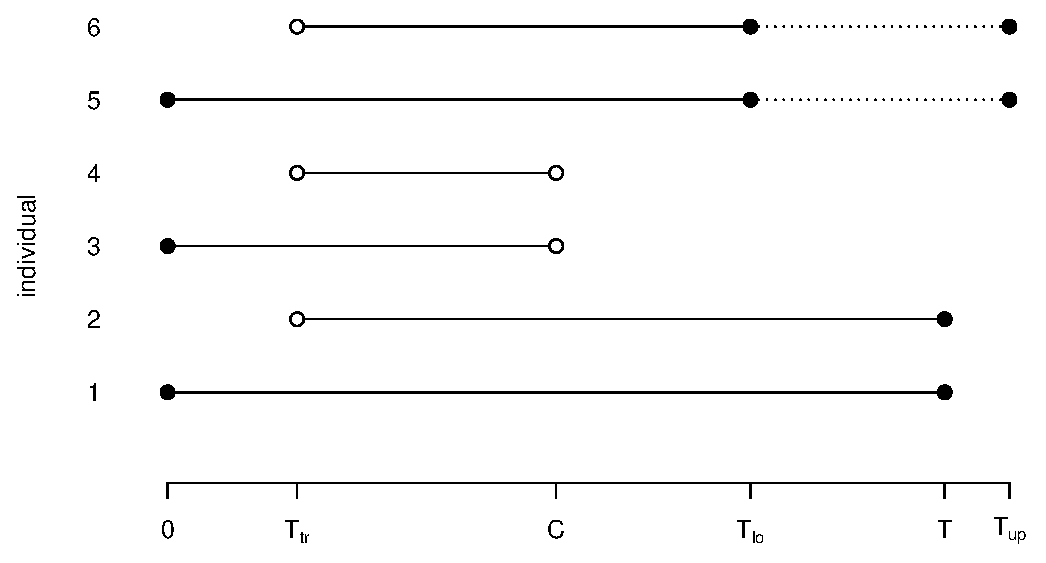
\epsfig{file=grafiken/censoringschemes.eps,scale=0.7}
{\it\caption{Illustration of different censoring
schemes.\label{censoringschemes}}}
\end{center}
\end{figure}

In a general framework an observation can now be uniquely described
 by the quadruple $(T_{tr},T_{lo},T_{up},\delta)$, with
\begin{center}
\begin{tabular}{ll}
$T_{lo}=T_{up}=T$, $\delta=1$ & if the observation is uncensored,\\
$T_{lo}=T_{up}=C$, $\delta=0$ & if the observation is right censored,\\
$T_{lo}<T_{up}$, $\delta=0$ & if the observation is interval censored.\\
\end{tabular}
\end{center}
For left truncated observations we have $T_{tr}>0$ while $T_{tr}=0$
for observations which are not truncated.

Based on these definitions we can now construct the likelihood
contributions for the different censoring schemes in terms of the
hazard rate $\lambda(t)$ and the survivor function
$S(t)=\exp(\int_0^t\lambda(u)du)$. Under the common assumption of
noninformative censoring and conditional independence, the
likelihood is given by
\begin{equation}\label{likelihood}
 L=\prod_{i=1}^n L_i,
\end{equation}
where
\[L_i = \lambda(T_{up})S(T_{up})/S(T_{tr}) = \lambda(T_{up})\exp\left(-\int_{T_{tr}}^{T_{up}}\lambda(t)dt\right)\]
for an uncensored observation,
\[L_i = S(T_{up})/S(T_{tr}) = \exp\left(-\int_{T_{tr}}^{T_{up}}\lambda(t)dt\right)\]
for a right censored observation and
\[L_i = (S(T_{lo})-S(T_{up}))/S(T_{tr}) = \exp\left(-\int_{T_{tr}}^{T_{lo}}\lambda(t)dt\right)\left(1-\exp\left(-\int_{T_{lo}}^{T_{up}}\lambda(t)dt\right)\right)\]
for an interval censored observation. Note that for explicit
evaluation of the likelihood (\ref{likelihood}) some numerical
integration technique has to be employed, since none of the
integrals can in general be solved analytically.

The above notation also allows for the easy inclusion of piecewise
constant, time-varying covariates via some data augmentation. Noting
that
\[\int_{T_{tr}}^{T}\lambda(t)dt = \int_{T_{tr}}^{t_1}\lambda(t)dt + \int_{t_1}^{t_2}\lambda(t)dt + \ldots + \int_{t_{p-1}}^{t_p}\lambda(t)dt + \int_{t_p}^{T}\lambda(t)dt\]
for $T_{tr}<t_1<\ldots<t_q<T$, we can replace an observation
$(T_{tr},T_{lo},T_{up},\delta)$ by a set of new observations
$(T_{tr},t_1,t_1,0)$, $(t_1,t_2,t_2,0)$, \ldots
$(t_{p-1},t_p,t_p,0)$, $(t_{p},T_{lo},T_{up},\delta)$ without
changing the likelihood. Therefore, observations with time-varying
covariates can be split up into several observations, where the
values $t_1<\ldots<t_p$ are defined by the changepoints of the
covariate and the covariate is now time-constant on each of the
intervals. In theory, other paths for a covariate $x(t)$ than
piecewise constant ones are also possible, if $x(t)$ is known for
$T_{tr}\le t\le T_{lo}$. In this case the the likelihood
(\ref{likelihood}) can also be evaluated numerically but a general
path $x(t)$ may lead to complicated data structures.

Figure \ref{timevaryingcovs} illustrates the data augmentation step
for a left truncated, uncensored observation and a covariate $x(t)$
that takes the three different values $x_1,x_2$ and $x_3$ on the
three intervals $[T_{tr},t_1], [t_1,t_2]$ and $[t_2,T_{up}]$. Here,
the original observation $(T_{tr},T_{up},T_{up},1)$ has to be
replaced by $(T_{tr},t_1,t_1,0)$, $(t_1,t_2,t_2,0)$ and
$(t_2,T_{up},T_{up},1)$.
\begin{figure}[htb]
\begin{center}
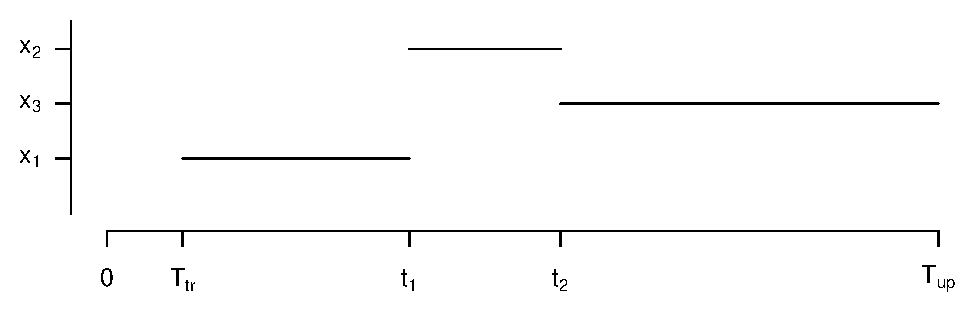
\epsfig{file=grafiken/timevaryingcovs.eps,scale=0.7}
{\it\caption{Illustration of time-varying
covariates.\label{timevaryingcovs}}}
\end{center}
\end{figure}

Currently, interval censored survival times can only be handled with
{\em remlreg objects}.

\subsection{Continuous-time multi-state models}\label{msmodels}
\index{Multi-state models}\index{Recurrent Events}\index{Disease
progression}\index{Competing risks}

Multi-state models are a flexible tool for the analysis of
time-continuous phenomena that can be characterized by a discrete
set of states. Such data structures naturally arise when observing a
discrete response variable for several individuals or objects over
time. Some common examples are depicted in Figure~\ref{some_msms} in
terms of their reachability graph for illustration. For recurrent
events (Figure~\ref{some_msms} (a)), the observations evolve through
time moving repeatedly between a fixed set of states. Other model
classes involve absorbing states, for example disease progression
models (Figure~\ref{some_msms} (b)), that are used to describe the
chronological development of a certain disease. If the severity of
this disease can be grouped into $q-1$ ordered stages of increasing
severity, a reasonable model might look like this: Starting from
disease state '$j$', an individual can only move to contiguous
states, i.e. either the disease gets worse and the individual moves
to state '$j+1$', or the disease attenuates and the individual moves
to state '$j-1$'. In addition, death is included as a further,
absorbing state '$q$', which can be reached from any of the disease
states. A model with several absorbing states is the competing risks
model (Figure~\ref{some_msms} (c)) where, for example, different
causes of death are analysed simultaneously.

\begin{figure}
\begin{center}
  \vspace{3mm}
 \mbox
 {
 \beginpicture
 \setcoordinatesystem units <0.65cm,0.65cm> point at 0 0
 \setlength{\unitlength}{0.65cm}

 \put {(a) Recurrent events} [Bl] at 0 16.5

 \put {\circle{1}} [Bl] at 7.5 12
 \put {\bf3} [Bl] at 7.35 11.85

 \put {\circle{1}} [Bl] at 5.5 14.5
 \put {\circle{1}} [Bl] at 9.5 14.5
 \put {\bf1} [Bl] at 5.35 14.35
 \put {\bf2} [Bl] at 9.35 14.35

 \arrow <3mm> [0.2,0.5] from 6.3 14.65 to 8.7 14.65
 \arrow <3mm> [0.2,0.5] from 8.7 14.35 to 6.3 14.35

 \arrow <3mm> [0.2,0.5] from  5.55 13.85 to 6.9 12.65
 \arrow <3mm> [0.2,0.5] from  7.25 12.65 to 5.9 13.85

 \arrow <3mm> [0.2,0.5] from  9.1 13.85 to 7.75 12.65
 \arrow <3mm> [0.2,0.5] from  8.1 12.65 to 9.45 13.85


 \put {(b) Disease progression} [Bl] at 0 10.5

 \put {\circle{1}} [Bl] at 7.5 6
 \put {$q$} [Bl] at 7.35 5.85

 \put {\circle{1}} [Bl] at 1.5 9
 \put {\circle{1}} [Bl] at 4.5 9
 \put {\circle{1}} [Bl] at 7.5 9
 \put {\circle{1}} [Bl] at 13.5 9
 \put {\bf1} [Bl] at 1.35 8.85
 \put {\bf2} [Bl] at 4.35 8.85
 \put {\bf3} [Bl] at 7.35 8.85
 \put {$q$-1} [Bl] at 13.15 8.85

 \put{$\cdots$} [Bl] at 10.1 8.9

 \arrow <3mm> [0.2,0.5] from 2.2 9.15 to 3.8 9.15
 \arrow <3mm> [0.2,0.5] from  3.8 8.85 to 2.2 8.85

 \arrow <3mm> [0.2,0.5] from 5.2 9.15 to 6.8 9.15
 \arrow <3mm> [0.2,0.5] from  6.8 8.85 to 5.2 8.85

 \arrow <3mm> [0.2,0.5] from 8.2 9.15 to 9.8 9.15
 \arrow <3mm> [0.2,0.5] from  9.8 8.85 to 8.2 8.85

 \arrow <3mm> [0.2,0.5] from 11.2 9.15 to 12.8 9.15
 \arrow <3mm> [0.2,0.5] from  12.8 8.85 to 11.2 8.85

 \arrow <3mm> [0.2,0.5] from  7.5 8.35 to 7.5 6.65
 \arrow <3mm> [0.2,0.5] from  4.75 8.35 to 7.0 6.65
 \arrow <3mm> [0.2,0.5] from  1.75 8.35 to 6.5 6.5
 \arrow <3mm> [0.2,0.5] from  13.25 8.35 to 8.5 6.5

 \put {(c) Competing risks} [Bl] at 0 4.5

 \put {\circle{1}} [Bl] at 1.5 0
 \put {\circle{1}} [Bl] at 4.5 0
 \put {\circle{1}} [Bl] at 7.5 0
 \put {\circle{1}} [Bl] at 13.5 0
 \put {\bf2} [Bl] at 1.35 -0.15
 \put {\bf3} [Bl] at 4.35 -0.15
 \put {\bf4} [Bl] at 7.35 -0.15
 \put {$q$} [Bl] at 13.35 -0.15

 \put {\circle{1}} [Bl] at 7.5 3
 \put {\bf1} [Bl] at 7.35 2.85

 \put{$\cdots$} [Bl] at 10.1 -0.1

 \arrow <3mm> [0.2,0.5] from  7.5 2.35 to 7.5 0.65

 \arrow <3mm> [0.2,0.5] from  6.9 2.6 to 4.75 0.65
 \arrow <3mm> [0.2,0.5] from  6.5 2.75 to 1.95 0.65
 \arrow <3mm> [0.2,0.5] from  8.5 2.75 to 12.85 0.65

 \endpicture
 }
 \vspace{3mm}

 \caption{Reachability graphs of some common multi-state
 models.\label{some_msms}}
\end{center}
\end{figure}

A multi-state model is fully described by a set of hazard rates
$\lambda_{hi}(t)$ where $h$, $h=1,\ldots,k$, indexes the type of the
transition and $i$, $i=1,\ldots,n$, indexes the individuals. Since
the hazard rates describe durations between transitions, we specify
them in analogy to hazard rate models for continuous time survival
analysis. To be more specific, $\lambda_{hi}(t)$ is modelled in a
multiplicative Cox-type way as
\[
 \lambda_{hi}(t) = \exp(\eta_{hi}(t)),
\]
where
\begin{equation}\label{addpred}
 \eta_{hi}(t) = g_{h0}(t) + \sum_{l=1}^Lg_{hl}(t)u_{il}(t) +
 \sum_{j=1}^Jf_{hj}(x_{ij}(t)) + v_i(t)'\gamma_h +  b_{hi}
\end{equation}
is an additive predictor consisting of the following components:
\begin{itemize}
 \item A time-varying, nonparametric baseline effect $g_{h0}(t)$ common for all
 observations.
 \item Covariates $u_{il}(t)$ with time-varying effects $g_{hl}(t)$.
 \item Nonparametric effects $f_{hj}(x_{ij}(t))$ of continuous covariates
 $x_{ij}(t)$.
 \item Parametric effects $\gamma_h$ of covariates $v_i(t)$.
 \item Frailty terms $b_{hi}$ to account for unobserved
 heterogeneity.
\end{itemize}

For each individual $i$, $i=1,\ldots,n,$ the likelihood contribution
in a multi-state model can be derived from a counting process
representation of the multi-state model. Let $N_{hi}(t)$,
$h=1,\ldots,k$ be a set of counting processes counting transitions
of type $h$ for individual $i$. Consequently, $h=1,\ldots,k$ indexes
the observable transitions in the model under consideration and the
jumps of the counting processes $N_{hi}(t)$ are defined by the
transition times of the corresponding multi-state process for
individual $i$.

From classical counting process theory (see e.g. \citeasnoun{Andetal93}, Ch.~VII.2), the intensity processes $\alpha_{hi}(t)$
of the counting processes $N_{hi}(t)$ are defined as the product of the hazard rate for type $h$ transitions $ \lambda_{hi}(t)$
and a predictable at-risk indicator process $Y_{hi}(t)$, i.e.
\[
 \alpha_{hi}(t) = Y_{hi}(t) \lambda_{hi}(t),
\]
where the hazard rates are constructed in terms of covariates as in
(\ref{addpred}). The at-risk indicator $Y_{hi}(t)$ takes the value
one if individual $i$ is at risk for a type $h$ transition at time
$t$ and zero otherwise. For example, in the multi-state model of
Figure~\ref{some_msms}a), an individual in state 2 is at risk for
both transitions to state 1 and state 3. Hence, the at-risk
indicators for both the transitions '2 to 1' and '2 to 3' will be
equal to one as long as the individual remains in state 2.

Under mild regularity conditions, the individual log-likelihood
contributions can now be obtained from counting process theory as
\begin{equation}\label{loglike1}
 l_i = \sum_{h=1}^k\left[ \int_0^{T_i}\log(\lambda_{hi}(t))dN_{hi}(t) -
 \int_0^{T_i}\lambda_{hi}(t)Y_{hi}(t)dt\right],
\end{equation}
where $T_i$ denotes the time until which individual $i$ has been
observed. The likelihood contributions can be interpreted similarly
as with hazard rate models for survival times (and in fact coincide
with these in the case of a multi-state process with only one
transition to an absorbing state). The first term corresponds to
contributions at the transition times since the integral with
respect to the counting process in fact equals a simple sum over the
transition times. Each of the summands is then given by the
log-intensity for the observed transition evaluated at this
particular time point. In survival models this term simply equals
the log-hazard evaluated at the survival time for uncensored
observations. The second term reflects cumulative intensities
integrated over accordant waiting periods between two successive
transitions. The integral is evaluated for all transitions the
corresponding person is at risk at during the current period. In
survival models there is only one such transition (the transition
from 'alive' to 'dead') and the integral is evaluated from the time
of entrance to the study to the survival or censoring time.

More details on multi-state models, including an exemplary analysis on human sleep, can be found in \citeasnoun{KneHen06}.

\section{Multilevel structured additive distributional and quantile regression}\label{distreg_star}

\subsection{Distributional regression}



Structured additive regression models assume that the distribution of the response variable $y$, given covariates $\xvec$ and $\uvec$, belongs to an exponential family. The conditional mean $\mu_i = E(y_i|\xvec,\uvec)$ is linked to a structured additive predictor
\begin{align*}
\eta_i = f_1(x_{i1}) + \ldots + f_p(x_{ip}) + \uvec_i' \gammavec, \,\,\,\,\,\,\,\, i = 1, \ldots, n,
\end{align*}
by $\mu_i = h(\eta_i)$, see Chapter \ref{obsmodel}. In matrix notation we obtain for the predictor
$$
\etavec = \Xvec_1 \betavec_1 + \ldots + \Xvec_p \betavec_p + \Uvec \gammavec,
$$
see again Chapter \ref{obsmodel} for details.
For the most basic model with Gaussian responses  and the  identity response function we have
\begin{align*}
y_i \sim  \mathcal{N}(\eta_i, \sigma^2) = \mathcal{N}(f_1(x_{i1}) + \ldots + f_p(x_{ip}) + \uvec_i' \gammavec,\sigma^2)
\end{align*}
or
$$
\yvec = \mathcal{N}(\etavec, \sigma^2 \Ivec) = \mathcal{N}(\Xvec_1 \betavec_1 + \ldots + \Xvec_p \betavec_p + \Uvec \gammavec,\sigma^2 \Ivec).
$$


Here and in other convential STAR models only the conditional mean is modeled in dependence of covariates.

A more flexible approach is given by distributional regression as introduced in  \citeasnoun{kleknelan14a} and \citeasnoun{kleknelan14b}. On the one hand, the class of distributions that can be estimated with distributional regression is no longer restricted to the exponential family. On the other hand, distributional regression allows to model not only the conditional mean of the response variable but the whole set of distribution parameters $\varthetavec_1,\ldots,\varthetavec_K$, i.e.~all $K$ parameters of the response distribution can be related to a set of predictor variables, which of course may vary between the different parameters. Using response functions $h_1, \ldots, h_K$ each of these parameters can be linked to a structured additive predictor via
\[
\varthetavec_k = h_k(\etavec_k) = h_k(\Xvec_{1k} \betavec_{1k} + \ldots + \Xvec_{pk} \betavec_{pk} + \Uvec_k \gammavec_k), \quad k=1,\ldots,K.
\]
Usually, the response functions are chosen to ensure appropriate restrictions on the parameter spaces. We use, for example, the exponential function to ensure positivity of the scale parameter.

Presumably the most simple distributional regression model is obtained with Gaussian responses where both the mean $\mu$ and the variance
$\sigma^2$ is modeled in terms of covariates.
Thus, we consider a regression model with
\begin{align*}
\begin{array}{lllll}
\muvec & = & h_1(\etavec_1) & = & \etavec_1, \\ [0.2cm]
\sigmavec^2 & = & h_2(\etavec_2) & = & \exp(\etavec_2).
\end{array}
\end{align*}

A possible generalization of the normal distribution is given by the three-parameter Student's t distribution with location parameter $\mu$, scale parameter $\sigma^2>0$ and degrees of freedom $\texttt{df}>0$. The probability density function is given by
\begin{align*}
f(y|\mu, \sigma, df) = \frac{\Gamma\left( \frac{df +1 }{2}\right)}{\sigma \Gamma\left( \frac{1}{2}\right) \Gamma\left(
\frac{df}{2}\right)\sqrt{df}} \cdot \left( 1+ \frac{(y-\mu)^2}{\sigma^2 df}\right)^{-\frac{df+1}{2}},
\end{align*}
where $\Gamma(x) = \int_0^{\infty} u^{x-1} \exp(-u) \mathrm{d}u$ for $x>0$ is the gamma function. Similar to the normal distribution the t distribution is symmetric and bell-shaped but it has heavier tails, offering a robust alternative to the normal distribution. For $\texttt{df} \rightarrow \infty$ it collapses to the normal distribution.

Regarding the positivity of $\sigma^2$ and $\texttt{df}$ we consider the model
\begin{align*}
\begin{array}{lllll}
\muvec & = & h_1(\etavec_1) & = & \etavec_1, \\ [0.2cm]
\sigmavec^2 & = & h_2(\etavec_2) & = & \exp(\etavec_2), \\ [0.2cm]
\boldsymbol{\texttt{df}} & = & h_3(\etavec_3) & = & \exp(\etavec_3). \\ [0.2cm]
\end{array}
\end{align*}

A popular two parameter distribution for modeling skewed distributions is the gamma distribution with mean parameter $\mu>0$ and shape parameter $\sigma>0$. The probability density function is given by
\begin{equation*}
f(y_i|\mu_i, \sigma_i) = \left( \frac{\sigma_i}{\mu_i} \right)^{\sigma_i} \cdot \frac{y_i^{\sigma_i-1}}{\Gamma(\sigma_i)} \cdot \exp\left(- \frac{\sigma_i}{\mu_i} \cdot y_i \right),
\end{equation*}
The mean of the gamma distribution corresponds to $\mu$, the variance is given by $\mu^2/\sigma$.
Setting up a regression model both the mean and the shape parameter are linked to a STAR predictor via the exponential function due to the positivity constraints:
\begin{align*}
\begin{array}{lllll}
\muvec & = & h_1(\etavec_1) & = & \exp(\etavec_1), \\ [0.2cm]
\sigmavec & = & h_2(\etavec_2) & = & \exp(\etavec_2).
\end{array}
\end{align*}

A comprehensive list of all distributional regression models available in BayesX can be found in Tables \ref{tab:distrBayesX1}  to \ref{tab:distrBayesX4} of the Reference Manual.


\subsection{Quantile Regression} \label{sec:quantreg}

 Distributional regression assumes a specific parametric probability distribution of the response (like the normal, lognormal or gamma distribution) and models some or all of its parameters in dependence of covariates. Quantile regression, in contrast, is a distribution-free approach, trying to directly model the different quantiles of the response as a function of covariates.

In linear quantile regression (see  \citeasnoun{Koe05}), we assume
\begin{align*}
q_{\varphi,i} = \beta_{\varphi,0} + \beta_{\varphi,1}x_{i1} + \ldots + \beta_{\varphi,p}x_{ip}
\end{align*}
where $q_\varphi$, for $\varphi \in (0,1)$, is the $\varphi$-quantile of the response distribution. Estimation of the quantile-specific regression coefficients $\betavec_{\varphi}$ relies on minimizing the asymmetrically weighted error (AWE) criterion
\begin{align}
\hat{\betavec}_{\varphi} = \mbox{argmin}_{\betavec_{\varphi}} \left\{ \sum_{i=1}^{n} \rho_{\varphi}(y_i - \xvec_i' \betavec_{\varphi})\right\},
\label{eq:quantmin}
\end{align}
with the loss function $\rho_{\varphi}$ defined by
\begin{align*}
\rho_{\varphi}(u) = \begin{cases} u \varphi & \textnormal{if $u \geq 0$} \\ u (\varphi - 1) & \textnormal{if $u < 0$,} \end{cases}
\end{align*}
which is also known as the check function. Since there exists no closed form solution for this minimization problem, estimates are typically obtained based on linear programming and modifications of the simplex algorithm, see \citeasnoun{Koe05} for details. The distribution of the response is implicitly determined by the estimated quantiles $q_{\varphi}$ provided that quantiles for a reasonable dense grid of $\varphi$-values are estimated. Generalizations to structured additive predictors are conceptually straightforward. However, estimation is highly challenging and almost impossible for complex hierarchical models, revealing the limits of frequentist quantile regression.

Bayesian structured quantile regression requires a distributional assumption for the responses to be able to set up a likelihood. Following \citeasnoun{WalKneLanYue12} we will assume independent and identically distributed observations following an asymmetric Laplace distribution with location parameter $\eta_{i,\varphi}$ (specified in the usual structured additive fashion), scale parameter $\sigma^2$ and skewness parameter $\varphi$,
\begin{align*}
y_{i} | \eta_{i,\varphi}, \sigma^2, \varphi \overset{\textnormal{iid}}{\sim} \textnormal{ALD}(\eta_{i,\varphi},\sigma^2,\varphi).
\end{align*}
Then, the density of the responses is given by
\begin{align*}
p(y_i | \eta_{i,\varphi},\sigma^2,\varphi) = \frac{\varphi(1-\varphi)}{\sigma^2} \exp\left(-\frac{\rho_{\varphi}(y_i - \eta_i{\varphi})}{\sigma^2}\right).
\end{align*}
Maximizing the corresponding posterior (for fixed $\sigma^2$ and $\varphi$) obviously is equivalent to minimizing the AWE criterion (\ref{eq:quantmin}) in case of a linear predictor. However, in contrast to frequentist quantile regression the linear predictor can be replaced by a hierarchical structured additive predictor without any further difficulties, see \citeasnoun{WalKneLanYue12} for details.

Since the check function $\rho_{\varphi}$ is non-differentiable, inference based on Markov chain Monte Carlo (MCMC) simulations at a first glance seems to be complicated. However, the asymmetric Laplace distribution can be represented as a scaled mixture of normals
\begin{align*}
Y_i = \eta_i + \xi W_i + \delta Z_i \sqrt{\sigma^2 W_i}
\end{align*}
with $\xi = \frac{1-2\varphi}{\varphi(1-\varphi)}$ and $\delta^2 = \frac{2}{\varphi(1-\varphi)}$.  $W_i \sim \textnormal{Exp}(\frac{1}{\sigma^2})$ and $Z_i \sim \mathcal{N}(0,1)$ are independent random variables following an exponential distribution with mean $\sigma^2$ and a standard normal distribution, respectively. Thus, using offsets $\xi W_i$ and weights $\delta \sqrt{\sigma^2 W_i}$ the Bayesian quantile regression problem can be interpreted as a conditionally Gaussian regression model after imputing $W_i$ as a part of the MCMC sampler.


\subsection{Multilevel models}
\label{star_multilevel}

Recently \citeasnoun{LanUml14} have proposed  a multilevel version of STAR models to cope with the hierarchical nature of many data sets.
Suppose that covariate $x_j \in \{1,\dots,K\}$ is a unit- or cluster index   and $x_{ij}$ indicates the cluster
observation $i$ pertains to.
Then the design  matrix $\mathbf{X}_j$ is a $n \times K$ incidence matrix with $\mathbf{X}_j[i,k] = 1$ if the $i$-th observation
belongs to cluster $k$ and zero else. The $K \times 1$ parameter vector $\boldsymbol{\beta}_j$ is the vector of regression parameters,
i.e.~the $k$-th element
in $\boldsymbol{\beta}_j$ corresponds to the regression coefficient of the $k$-th cluster.
We now define a second level equation
\begin{equation}
\label{eq:compprior}
\boldsymbol{\beta}_j = \boldsymbol{\eta}_j + \boldsymbol{\varepsilon}_j =
\mathbf{X}_{j1} \boldsymbol{\beta}_{j1} + \ldots + \mathbf{X}_{jp_j} \boldsymbol{\beta}_{jp_j} +
\mathbf{U}_j \boldsymbol{\gamma}_j +  \boldsymbol{\varepsilon}_j,
\end{equation}
where the terms $\mathbf{X}_{j1} \boldsymbol{\beta}_{j1},\dots,\mathbf{X}_{jp_j} \boldsymbol{\beta}_{jp_j}$ correspond to additional nonlinear
functions $f_{j1},\dots,f_{jp_j}$ and
$\mathbf{U}_j \boldsymbol{\gamma}_j$ comprises additional linear effects of cluster level covariates.
The ``errors'' $\boldsymbol{\varepsilon}_j \sim N(\mathbf{0}, \tau^2_j \mathbf{I})$
comprise a vector of i.i.d.\ Gaussian random effects.
Using the compound prior (\ref{eq:compprior}) we obtain an additive
decomposition of the cluster specific effect. By allowing a full STAR predictor (as in the level-1 equation), a rather complex decomposition of
the cluster effect
$\boldsymbol{\beta}_j$ including interactions is possible. A special case arises if cluster specific covariates are not available. Then the
prior for $\boldsymbol{\beta}_j$ collapses to
$\boldsymbol{\beta}_j = \boldsymbol{\varepsilon}_j \sim N(\mathbf{0}, \tau^2_j \mathbf{I})$ and we obtain a simple i.i.d. Gaussian cluster
specific random effect with variance parameter $\tau^2_j$.

A third or fourth level in the hierarchy is possible by assuming that the second or third level regressions
contain additional cluster-specific random effects whose parameters are again modeled through  STAR predictors of cluster level covariates.



%In a multilevel STAR model (\shortciteN{lanuml14}) the regression coefficients $\betavec_j$ of a function $f_j$ may themselves obey a regression model with a structured additive predictor, i.e.
%\begin{align}
%\betavec_j \sim  \mathcal{N}(\boldsymbol{\eta}_j,\tau^2_j \mathbf{I}) =
%\mathcal{N}(\Zvec_{j1} \betavec_{j1} + \ldots + \Zvec_{jq_j} \betavec_{jq_j} + \Xvec_j \gammavec_j, \tau^2_j \mathbf{I})
%\label{eq:compprior}
%\end{align}
%where the terms $\mathbf{Z}_{j1} \boldsymbol{\beta}_{j1},\dots,\mathbf{Z}_{jq_j} \boldsymbol{\beta}_{jq_j}$ represent additional nonlinear functions $f_{j1},\dots,f_{jq_j}$, and  $\mathbf{X}_j \boldsymbol{\gamma}_j$ comprises additional linear effects.
%Further levels are possible by assuming that the second level regression parameters $\boldsymbol{\beta}_{jl}$, \linebreak $l=1,\dots,q_j$, again obey a STAR model.
%
%In this paper we use the compound prior (\ref{eq:compprior}) if a covariate $z_j \in \{1,\dots,K\}$ is a spatial index and $z_{ij}$ indicates the region observation $i$ pertains to. Then, the design matrix $\mathbf{Z}_j$ is a $n \times K$ incidence matrix with $\mathbf{Z}_j[i,k] = 1$ if the $i$-th observation belongs to region $k$ and zero else. The $K \times 1$ parameter vector $\boldsymbol{\beta}_j$ is the vector of regression parameters, i.e.~the $k$-th element in $\boldsymbol{\beta}$ corresponds to the regression coefficient of the $k$-th region. The use of the compound prior (\ref{eq:compprior}) allows for further explaining the region specific effect by spatial covariates.
%
%The hierarchical structure of the Austrian political-administrative units suggests a four level regression model: Single-family homes (level-1) belong to municipalities (level-2), which are nested in districts (level-3), which are themselves nested in counties (level-4). Assuming house prices per square meter to be normally distributed leads to the following four level STAR model, see also  \shortciteN{brulan11}:
%\begin{align}
%\begin{array}{llll}
%\mbox{level-1:} & \mathit{\boldsymbol{p_{qm}}} &  = & \fvec_1(\mathit{area}) + \fvec_2(\mathit{area\_plot}) + \fvec_3(\mathit{age}) + \fvec_4(\mathit{time\_index}) + \\
%                &              &    & \fvec_5(\mathit{muni}) + \Xvec \gammavec + \varepsilonvec \\
%                &              &  = & \Zvec_1 \betavec_1 + \Zvec_2 \betavec_2 + \Zvec_3 \betavec_3 + \Zvec_4 \betavec_4 + \Zvec_5 \betavec_5 + \Xvec \gammavec + \varepsilonvec  \\ [0.2cm]
%\mbox{level-2:} & \betavec_5   &  = & \fvec_{5,1}(\mathit{pp\_ind}) + \fvec_{5,2}(\mathit{ln\_educ}) +  \fvec_{5,3}(\mathit{age\_ind}) + \fvec_{5,4}(\mathit{comm}) + \\
%                &              &    & \fvec_{5,5}(\mathit{ln\_den}) + \fvec_{5,6}(\mathit{dist}) + \varepsilonvec_5      \\
%                &              &  = & \Zvec_{5,1} \betavec_{5,1} + \Zvec_{5,2} \betavec_{5,2} + \Zvec_{5,3} \betavec_{5,3} + \Zvec_{5,4} \betavec_{5,4} +  \\
%                &              &    & \Zvec_{5,5} \betavec_{5,5} + \Zvec_{5,6} \betavec_{5,6} + \varepsilonvec_5  \\ [0.2cm]
%\mbox{level-3:} & \betavec_{5,6} & = & \fvec_{5,6,1}(\mathit{wko\_ind}) + \fvec_{5,6,2}^{mrf}(\mathit{dist}) + \fvec_{5,6,3}(\mathit{county}) + \varepsilonvec_{5,6} \\
%                &                & = & \Zvec_{5,6,1} \betavec_{5,6,1} + \Zvec_{5,6,2} \betavec_{5,6,2} + \Zvec_{5,6,3} \betavec_{5,6,3} + \varepsilonvec_{5,6} \\ [0.2cm]
%\mbox{level-4:} & \betavec_{5,6,3} & = & \mathds{1} \gamma_0 + \varepsilonvec_{5,6,3}. \\
%\end{array}
%\label{eq:model}
%\end{align}
%
%The categorical covariates on level-1, describing the quality and equipment of the house, are encoded as dummy variables and subsumed in the design matrix $\Xvec$ with estimated parameters $\gammavec$. The possibly nonlinear functions $\fvec_1,\fvec_2,\dots$ are modeled by P-splines.
%
%The level-1 equation contains an uncorrelated random municipality effect $f_5(\emph{muni})$, controlling for unordered spatial heterogeneity. This municipality-specific heterogeneity is modeled through the level-2 equation and is further decomposed into a district and finally into a county level effect (levels 3 and 4). Furthermore, district specific spatial heterogeneity is modeled through a correlated spatial effect $f_{5,6}(\emph{dist})$ in the level-3 equation by Markov random fields, denoted by the superscript "\emph{mrf}", see \shortciteN{fahkne13} for details regarding MRF's.
%
%From model (\ref{eq:model}) we immediately get the conditional mean of the house price per square meter $p_{qm}$. The $\varphi$-th conditional quantile of the house price per square meter is given by
%\begin{equation}
%Q_{\varphi}(p_{qm}) = \EV(p_{qm}) + \sigma \cdot \Phi^{-1}(\varphi),
%\label{eq:quantnormal}
%\end{equation}
%with $\Phi^{-1}(\varphi)$ being the $\varphi$-th quantile of the standard normal distribution. The variance parameter $\sigma^2$ (and so the standard deviation $\sigma$) can be replaced by a suitable estimator.
%%by the sample variance
%%\begin{align*}
%%\widehat{\sigma^2} = S^2 = \frac{\sum_{i=1}^n (p_{qm_i}-\widehat{p_{qm_i}})^2}{n-k},
%%\end{align*}
%%where $k$ denotes the total degrees of freedom.
%Equation (\ref{eq:quantnormal}) shows that the quantiles can be received by simply shifting the mean according to the estimated variance.
%
%Due to the additive structure of our model the conditional quantiles of the house price per square meter change additively with changes in values of covariates. Subsequently, the conditional quantiles of the total house price $p$ change proportionally to the floor area of the building:
%\begin{align*}
%\begin{array}{lll}
%Q_{\varphi}(p) & = & area \cdot \left(\eta + \sigma \cdot \Phi^{-1}(\varphi)\right)\\ [0.2cm]
%     & = & area \cdot \left(f_1(area)+ \ldots + f_5(muni)+\gamma_1 x_1 + \ldots  +\gamma_p x_p + \sigma \cdot \Phi^{-1}(\varphi)\right).
%\end{array}
%\end{align*}
%
%Therefore, if for example covariate $x_1$ changes by one unit, the predictor $\eta$ -- and so the considered quantile of the price per square meter -- changes additively by $\gamma_1$. The quantile of the total price then changes by $area \cdot \gamma_1$. Thus, the change in the quantiles of the price is proportional to the floor area of the building. Turning to the nonlinear effects, let $f(z)$ be the nonlinear effect of a covariate $z$, and let $\mathrm{d}f(z) = f(z+1) - f(z)$. Then, analogously, the quantile of the price per square meter changes by $\mathrm{d}f(z)$ and the quantile of the total price changes by $area \cdot \mathrm{d}f(z)$, again being proportional to the size of the house. Furthermore, since $f(.)$ is a nonlinear function, the change differs over the range of $z$. For the conditional mean we get analog results.
%%\subsubsection*{Lognormally distributed prices}
%%
%%In Section \ref{sec:data} we have seen that the empirical house prices per square meter seem to be approximately lognormally distributed instead of being Gaussian. Assuming the response \emph{$p_{qm}$} to be lognormally distributed, i.e.
%%\begin{align*}
%%\mathit{p_{qm}} \sim \mathcal{LN}(\mu, \sigma^2),
%%\end{align*}
%%leads to normally distributed logged house prices per square meter. Thus, one could guess to improve model (\ref{eq:model}) by replacing the response \emph{$p_{qm}$} by the logged house price per square meter \emph{$lnp_{qm}$}, i.e.
%%\begin{align}
%%\mathit{\boldsymbol{lnp_{qm}}} = \boldsymbol{\eta} + \varepsilonvec,
%%\label{eq:model2}
%%\end{align}
%%which we will call the \emph{Loggaussian model}, with the same hierarchical predictor $\boldsymbol{\eta}$ as before and the errors again being mutually independent normally distributed with mean $0$ and variance $\sigma^2$.
%
%For the loggausian model (\ref{loggaussianm})
%We receive the conditional quantiles of the house price per square meter by
%$$
%\begin{array}{lll}
%Q_{\varphi}(p_{qm}) & = & \exp\left(\eta + \sigma \cdot \Phi^{-1}(\varphi)\right) \\ [0.2cm]
%     & = & \exp\left(f_1(area)+ \ldots + f_5(muni)+\gamma_1 x_1 + \ldots  + \gamma_p x_p + \sigma \cdot \Phi^{-1}(\varphi)\right) \\ [0.2cm]
%     & = & \exp\left(f_1(area)\right) \ldots \exp\left(f_5(muni)\right) \exp(\gamma_1 x_1)  \ldots  \exp(\gamma_p x_p) \exp(\sigma \cdot \Phi^{-1}(\varphi)).
%\end{array}
%$$
%
%Obviously, the conditional quantiles of the house price per square meter $p_{qm}$ now change multiplicatively with changes in values of covariates. If for example covariate $x_1$ changes by one unit, the predictor $\eta$ again changes by $\gamma_1$, but the quantiles of the price per square meter now change multiplicatively by the factor $\exp(\gamma_1)$, yielding
%$$
%\begin{array}{lll}
%\Delta Q_{\varphi}(p_{qm}) & = & \exp(\eta + \sigma \cdot \Phi^{-1}(\varphi)) \cdot \exp(\gamma_1) - \exp(\eta + \sigma \cdot \Phi^{-1}(\varphi))\\ [0.2cm]
%     & = & \exp(\eta + \sigma \cdot \Phi^{-1}(\varphi)) \cdot \left(\exp(\gamma_1)-1\right).
%\end{array}
%$$
%For the conditional quantiles of the total prices we get:
%$$
%\begin{array}{lll}
%Q_{\varphi}(p) & = & area \cdot \exp(\eta + \sigma \cdot \Phi^{-1}(\varphi)) \\ [0.2cm]
%     & = & area \cdot \exp\left(f_1(area)\right) \ldots \exp\left(f_5(muni)\right) \exp(\gamma_1 x_1)  \ldots  \exp(\gamma_p x_p) \exp(\sigma \cdot \Phi^{-1}(\varphi)).
%\end{array}
%$$
%
%So, the quantiles of the total price change multiplicatively with changes in values of covariates too. If for example covariate $x_1$ changes by one unit, the quantiles of the total price change by
%\begin{align*}
%\Delta Q_{\varphi}(p) = area \cdot \exp(\eta + \sigma \cdot \Phi^{-1}(\varphi)) \cdot \left(\exp(\gamma_1)-1\right),
%\end{align*}
%making the change again proportional to the floor area. Similarly, if covariate $z$ (representing a nonlinear effect) changes by one unit, both the conditional quantiles of prices per square meter and the conditional quantiles of total prices multiplicatively change by the factor $\exp\left(\mathrm{d}f(z)\right)$, since
%$$
%\exp\left(f(z+1)\right) = \exp\left(f(z+1)-f(z)+f(z)\right) = \exp\left(\mathrm{d}f(z)\right)\exp\left(f(z)\right).
%$$
%Therefore, the change in the quantiles of total prices caused by a change in any covariate again is proportional to the floor area of the building.
%
%
%For the conditional mean of the house price per square meter
%\begin{align*}
%\EV(p_{qm}) = \exp(\eta + \sigma^2/2)
%\end{align*}
%we get analog results.
%




\addcontentsline{toc}{section}{Bibliography}

\begin{thebibliography}{99}


\harvarditem{Albert \& Chib}{1993}{AlbChi93}
 {\scshape Albert, J. \& Chib, S.} (1993).
 Bayesian Analysis of Binary and Polychotomous Response Data.
 {\it Journal of the American Statistical Association}, {\bf 88}, 669--679.

\harvarditem{Andersen et al.}{1993}{Andetal93}
 {\scshape Andersen, P. K., Borgan, {\O}, Gill, R. D. \& Keiding, N.} (1993).
 {\it Statistical Models Based on Counting Processes.}
 New York: Springer Verlag.

\harvarditem{Andrews \& Mallows}{1974}{AndMal74}
 {\scshape Andrews, D. F. \& Mallows, C. L.} (1974).
 Scale mixtures of Normal Distributions.
 {\it Journal of the Royal Statistical Society B}, {\bf 36}, 99--102.

\harvarditem{Bollaerts, Eilers \& van Mechelen}{2006}{BolEilvMe06}
 {\scshape Albert, J. \& Chib, S.} (1993).
 Simple and Multiple P-Spline Regression with Shape Constraints.
 {\it British Journal of Mathematical and Statistical Psychology}, {\bf 59}, 451--469.

\harvarditem{Belitz}{2007}{Bel07}
 {\scshape Belitz, C.} (2007).
 {\it Model Selection in Generalized Structured Additive Regression Models.}
 PhD Thesis, University of Munich.

\harvarditem{Belitz \& Lang}{2008}{BelLan08}
{\scshape Belitz, C. \& Lang, S.} (2008).
 Simultaneous Selection of Variables and Smoothing Parameters in Structured Additive Regression Models.
{\it Computational Statistics and Data Analysis}, {\bf 53} , 61-81.

\harvarditem{Besag, York \& Molli\'{e}}{1991}{BesYorMol91}
 {\scshape Besag, J., York, J. \& Molli\'{e}, A.} (1991).
 Bayesian Image Restoration with two Applications in Spatial Statistics (with discussion).
 {\it Annals of the Institute of Statistical Mathematics}, {\bf 43}, 1--59.

\harvarditem{Brezger \& Lang}{2006}{BreLan06}
 {\scshape Brezger, A. \& Lang, S.} (2006).
 Generalized Additive Regression based on Bayesian P-Splines.
 {\it Computational Statistics and Data Analysis} {\bf 50}, 967--991.

\harvarditem{Devroye}{1986}{Dev86}
 {\scshape Devroye, L.} (1986).
 {\it Non-Uniform Random Variate Generation.}
 New York: Springer Verlag.

\harvarditem{Eilers \& Marx}{1996}{EilMar96}
 {\scshape Eilers, P. H. C. \& Marx, B. D.} (1996).
 Flexible Smoothing using B-Splines and Penalized Likelihood (with comments and rejoinder).
 {\it Statistical Science}, {\bf 11}, 89--121.

\harvarditem{Fahrmeir, Kneib \& Lang}{2004}{FahKneLan04}
 {\scshape Fahrmeir, L., Kneib, T. \& Lang, S.} (2004).
 Penalized Structured Additive regression for Space-Time Data: A Bayesian Perspective.
 {\it Statistica Sinica}, {\bf 14}, 715--745.

\harvarditem{Fahrmeir et al.}(2013){fahkne13}
{\scshape Fahrmeir, L.,  Kneib, T., Lang, S. \& Marx, B.}{2013}
{\it Regression: Models, Methods and Applications.}
 New York: Springer-Verlag.


\harvarditem{Fahrmeir \& Lang}{2001}{FahLan01a}
 {\scshape Fahrmeir, L. \& Lang, S.} (2001a).
 Bayesian Inference for Generalized Additive Mixed Models Based on Markov Random Field Priors.
 {\it Journal of the Royal Statistical Society C}, {\bf 50}, 201--220.

\harvarditem{Fahrmeir \& Lang}{2001}{FahLan01b}
 {\scshape Fahrmeir, L. \& Lang, S.} (2001b).
 Bayesian Semiparametric Regression Analysis of Multicategorical Time-Space Data.
 {\it Annals of the Institute of Statistical Mathematics}, {\bf 53}, 10--30.

\harvarditem{Fahrmeir \& Osuna}{2006}{FahOsu06}
 {\scshape Fahrmeir, L. \& Osuna, L.} (2006).
 Structured Additive Regression for Overdispersed and Zero-Inflated Count Data.
 {\it Applied Stochastic Models in Business and Industry}, {\bf 22}, 351--369

 \harvarditem{Fahrmeir \& Tutz}{2001}{FahTut01}
 {\scshape Fahrmeir, L. \& Tutz, G.} (2001).
 {\it Multivariate Statistical Modelling based on Generalized Linear Models.}
 New York: Springer-Verlag.

\harvarditem{Fotheringham, Brunsdon \& Charlton}{2002}{FotBruCha02}
 {\scshape Fotheringham, A. S., Brunsdon, C., \& Charlton, M. E.} (2002).
 {\it Geographically Weighted Regression: The Analysis of Spatially Varying Relationships.}
 Chichester: Wiley.

\harvarditem{Gamerman}{1997}{Gam97}
 {\scshape Gamerman, D.} (1997).
 Efficient Sampling from the Posterior Distribution in Generalized Linear Models.
 {\it Statistics and Computing}, {\bf 7}, 57--68.

\harvarditem{Gelfand, Sahu \& Carlin}{1996}{GelSahCar96}
 {\scshape Gelfand, A. E., Sahu, S. K. \& Carlin, B. P.} (1996).
 Efficient Parametrizations for Genera\-lized Linear Mixed Models.
 In: Bernardo, J. M., Berger, J. O., Dawid, A. P. \& Smith, A. F. M. (eds.),
 {\it Bayesian Statistics 5}, 165--180.
 Oxford University Press.

\harvarditem{George \& Liu}{1981}{GeoLiu81}
 {\scshape George, A. \& Liu, J.W.} (1981).
 {\it Computer Solution of Large Sparse Positive Definite Systems.}
 Series in computational mathematics, Prentice-Hall.

\harvarditem{Green}{1987}{Gre87}
 {\scshape Green, P. J.} (1987).
 Penalized Likelihood for General Semiparametric Regression Models.
 {\it International Statistical Review}, {\bf 55}, 245--259.

\harvarditem{Green}{2001}{Gre01}
 {\scshape Green, P. J.} (2001).
 A Primer in Markov Chain Monte Carlo.
 In: Barndorff-Nielsen, O. E., Cox, D. R. \& Kl\"{u}ppelberg, C. (eds.),
 {\it Complex Stochastic Systems}, 1--62.
 Chapmann and Hall, London.

\harvarditem{Green \& Silverman}{1994}{GreSil94}
 {\scshape Green, P. J. \& Silverman, B.} (1994).
 {\it Nonparametric Regression and Generalized Linear Models.}
 Chapman and Hall, London.

\harvarditem{Griffin \& Brown}{2005}{GriBro05}
 {\scshape Griffin, J. E., and Brown, P. J.} (2005). Alternative Prior Distributions
 for Variable Selection with very many more Variables than Observations. Technical
 report, University of Warwick, Dept. of Statistics.

\harvarditem{Harville}{1977}{Har77}
 {\scshape Harville, D. A.} (1977).
 Maximum Likelihood Approaches to Variance Component Estimation and to related Problems.
 {\it Journal of the American Statistical Association}, {\bf 72}, 320--338.

\harvarditem{Hastie \& Tibshirani}{1990}{HasTib90}
 {\scshape Hastie, T. \& Tibshirani, R.} (1990).
 {\it Generalized Additive Models.}
 Chapman and Hall, London.

\harvarditem{Hastie \& Tibshirani}{1993}{HasTib93}
 {\scshape Hastie, T. \& Tibshirani, R.} (1993).
 Varying-Coefficient Models.
 {\it Journal of the Royal Statistical Society B}, {\bf 55}, 757--796.

\harvarditem{Hastie \& Tibshirani}{2000}{HasTib00}
 {\scshape Hastie, T. \& Tibshirani, R.} (2000).
 Bayesian Backfitting.
 {\it Statistical Science}, {\bf 15}, 193--223.

\harvarditem{Hastie, Tibshirani \& Firedman}{2001}{HasTibFri01}
 {\scshape Hastie, T., Tisbshirani, R. \& Friedman, J.} (2001).
 {\it The Elements of Statistical Learning: Data Mining, Inference and Prediction.}
 New York: Springer-Verlag.

\harvarditem{Hennerfeind, Brezger \& Fahrmeir}{2006}{HenBreFah06}
 {\scshape Hennerfeind, A., Brezger, A. \& Fahrmeir, L.} (2006).
 Geoadditive Survival Models.
 {\it Journal of the American Statistical Association}, {\bf 101}, 1065--1075.

\harvarditem{Holmes \& Held}{2006}{HolHel06}
 {\scshape Holmes, C., Held, L.} (2006).
 Bayesian Auxiliary Variable Models for Binary and Multinomial Regression.
 {\it Bayesian Analysis}, {\bf 1}, 145--168.

\harvarditem{Hurvich, Simonoff \& Tsai}{1998}{HurSimTsa98}
 {\scshape Hurvich, C. M., Simonoff, J. S. \& Tsai, C. L.} (1998).
 Smoothing Parameter Selection in Nonparametric Regression using an improved {A}kaike Information Criterion.
 {\it Journal of the Royal Statistical Society B}, {\bf 60}, 271--293.

\harvarditem{Ishwaran \& Rao}{2005}{IshRao05}
 {\scshape Ishwaran, H., and Rao, S. J.} (2005). Spike and Slab Variable
 Selection: Frequentist and Bayesian Strategies. {\it The Annals of Statistics},
 {\bf 33}, 730-773.

\harvarditem{Johnson, Moore \& Ylvisaker}{1990}{JohMooYlv90}
 {\scshape Johnson, M.E., Moore, L.M. \& Ylvisaker, D.} (1990).
 Minimax and Maximin Designs.
 {\it Journal of Statistical Planning and Inference}, {\bf 26}, 131--148.

\harvarditem{Kammann \& Wand}{2003}{KamWan03}
 {\scshape Kammann, E. E. \& Wand, M. P.} (2003).
 Geoadditive Models.
 {\it Journal of the Royal Statistical Society C}, {\bf 52}, 1--18.


\harvarditem{Klein et al.}{2014a}{KleDenKneLan14}
{\scshape Klein, N., Denuit, M., Kneib, T. \& Lang, S.}(2014).
Nonlife Ratemaking and Risk Management with Bayesian additive Models for Location, Scale and Shape.
{\it Insurance: Mathematics and Economics}, {\bf 55}, 225--249.


\harvarditem{Klein et al.}{2014b}{kleknelan14a}
{\scshape Klein, N., Kneib, T., Lang, S.}(2013).
Bayesian Structured Additive Distributional Regression.
{\it Under revision for Annals of Applied Statistics}.


\harvarditem{Klein, Kneib \& Lang}{2014}{kleknelan14b}
{\scshape Klein, N., Kneib, T. \& Lang, S.}(2014).
Bayesian Generalized Additive Models for Location, Scale and Shape for Zero-Inflated and Overdispersed Count Data.
To appear in {\it Journal of the American Statistical Association}, doi:10.1080/01621459.2014.912955.


\harvarditem{Klein et al.}{2014c}{KleKneLan14c}
{\scshape Klein, N., Kneib, T., Klasen, S. \& Lang, S.}(2014).
Bayesian Structured Additive Distributional Regression for Multivariate Responses.
To appear in {\it Journal of the Royal Statistical Society C}, doi:10.1111/rssc.12090.


\harvarditem{Koenker}{2005}{Koe05}
{\scshape Koenker, R.}(2005).
{\it Quantile Regression.}
Cambridge University Press, New York.



\harvarditem{Kneib}{2006}{Kne06}
 {\scshape Kneib, T.} (2006).
 Geoadditive Hazard Regression for Interval Censored Survival Times.
 {\it Computational Statistics and Data Analysis}, {\bf 51}, 777--792

\harvarditem{Kneib \& Hennerfeind}{2006}{KneHen06}
 {\scshape Kneib, T. \& Hennerfeind, A.} (2006).
 Bayesian Semiparametric Multi-State Models.
 {\it Statistical Modelling}, {\bf 8}, 169--198.

\harvarditem{Kneib \& Fahrmeir}{2006}{KneFah06}
 {\scshape Kneib, T. \& Fahrmeir, L.} (2006).
 Structured Additive Regression for Categorical Space-Time Data: A Mixed Model approach.
 {\it Biometrics}, {\bf 62}, 109--118.

\harvarditem{Kneib \& Fahrmeir}{2007}{KneFah07}
 {\scshape Kneib, T. \& Fahrmeir, L.} (2007).
 A Mixed Model Approach to Structured Hazard Regression.
 {\it Scandinavian Journal of Statistics}, {\bf 34}, 207--228.

\harvarditem{Kneib et al.}{2009}{Kne09}
 {\scshape Kneib, T., Konrath, S. und Fahrmeir, L.} (2009). High-dimensional
 Structured Additive Regression Models: Bayesian Regularisation, Smoothing and Predictive
 Performance. Department of Statistics, Technical Report No. 46, LMU Munich.

\harvarditem{Knorr-Held}{1999}{KnoHel99}
 {\scshape Knorr-Held, L.} (1999).
 Conditional Prior Proposals in Dynamic Models.
 {\it Scandinavian Journal of Statistics}, {\bf 26}, 129--144.

\harvarditem{Konrath et al.}{2008}{Kon08}
 {\scshape Konrath, S., Kneib, T., Fahrmeir, L.} (2008). Bayesian Regularisation
 in Structured Additive Regression Models for Survival Data. Department of Statistics,
 Technical Report No.35, LMU Munich.

\harvarditem{Lang \& Brezger}{2004}{LanBre04}
 {\scshape Lang, S. \& Brezger, A.} (2004).
 Bayesian P-Splines.
 {\it Journal of Computational and Graphical Statistics}, {\bf 13}, 183--212.

\harvarditem{Lang et al.}{2014}{LanUml14}
 {\scshape Lang, S., Umlauf, N., Wechselberger, P., Harttgen, K.  \& Kneib, T.} (2014).
 Multilevel Structured Additive Regression.
 {\it Statistics and Computing}, {\bf 24}, 223--238.


\harvarditem{Lin \& Zhang}{1999}{LinZha99}
 {\scshape Lin, X. \& Zhang, D.} (1999).
 Inference in Generalized Additive Mixed Models by using Smoothing Splines.
 {\it Journal of the Royal Statistical Society B}, {\bf 61}, 381--400.

\harvarditem{McCullagh \& Nelder}{1989}{McCNel89}
 {\scshape McCullagh, P. \& Nelder, J. A.} (1989).
 {\it Generalized Linear Models.}
 Chapman and Hall, London.

\harvarditem{M\"{u}ller, Stadtm\"{u}ller \& Tabnak}{1997}{MueStaTab97}
 {\scshape M\"{u}ller, H. G., Stadtm\"{u}ller, U. \& Tabnak, F.} (1997).
 Spatial Smoothing of Geographically Aggregated Data, with Applications to the Construction of Incidence Maps.
 {\it Journal of the American Statistical Association} {\bf 92}, 61--71.

\harvarditem{Nychka \& Saltzman}{1998}{NycSal98}
 {\scshape Nychka, D. \& Saltzman, N.} (1998).
 {\it Design of Air-Quality Monitoring Networks.}
 Lecture Notes in Statistics, 132, 51--76.

\harvarditem{Osuna}{2004}{Osu04}
 {\scshape Osuna, L.} (2004)
 {\it Semiparametric Bayesian Count Data Models}.
 Dr. Hut Verlag, M\"{u}nchen.

\harvarditem{Park \& Casella}{2008}{ParCas08}
 {\scshape Park, T., and Casella, G.} (2008). The Bayesian Lasso.
 {\it Journal of the American Statistical Association}, {\bf 482}, 681-686.

\harvarditem{Rue}{2001}{Rue01}
 {\scshape Rue, H.} (2001).
 Fast Sampling of Gaussian Markov Random Fields with Applications.
 {\it Journal of the Royal Statistical Society B}, {\bf 63}, 325--338.

\harvarditem{Ruppert, Wand \& Carroll}{2003}{RupWanCar03}
 {\scshape Ruppert, D., Wand, M. P. \& Carroll, R. J.} (2003).
 {\it Semiparametric Regression.}
 Cambridge University Press.

\harvarditem{Spiegelhalter et al.}{2002}{SpiBesCar02}
 {\scshape Spiegelhalter, D. J., Best, N. G., Carlin, B. P. \& van der Linde, A.} (2002).
 Bayesian Measures of Model Complexity and Fit.
 {\it Journal of the Royal Statistical Society B}, {\bf 65}, 583--639.

\harvarditem {Waldmann et al.}{2013}{WalKneLanYue12}
{\scshape Waldmann, E. and Kneib, T. and Lang, S. and Yue, Y.}(2013)
Bayesian Semiparametric Additive  Quantile Regression.
{\it Statistical Modelling}, {\bf 13}, 223--252.



\end{thebibliography}

\addcontentsline{toc}{section}{Index}
\documentclass[11pt,a4paper,twoside]{bayesxarticle}


\usepackage{amsfonts}
\usepackage[dvips]{graphicx}
\usepackage[dvips]{epsfig}
\usepackage{fancyhdr}
\usepackage{dsfont}
\usepackage{amsmath}
\usepackage{dsfont}
\usepackage{amssymb}

%\usepackage{showkeys}
%\usepackage{showidx}

\usepackage{rotating}
\usepackage{shortvrb}
\usepackage{multicol}
\usepackage{longtable}
\usepackage{xr}

\usepackage[ps2pdf]{thumbpdf}
\usepackage[ps2pdf]{hyperref}

\input{prepictex}
\input{pictexwd}
\input{postpictex}

\hypersetup{
%    pdffitwindow=true,
    pdfstartview=FitB,
    pdftitle={BayesX Manuals},
    pdfauthor={Christiane Belitz, Andreas Brezger, Nadja Klein, Thomas Kneib, Stefan Lang and Nikolaus Umlauf},
    colorlinks=true,
    linkcolor=blue,
    pdfpagemode=UseOutlines,
    bookmarksopen=true,
    bookmarksnumbered=true,
    pdfstartpage={1},
    hyperindex=true
    }

\usepackage[dcu]{harvard}

\sloppy
\parindent0em
\parskip0.3em
\topmargin -0.3cm \textheight24cm \textwidth16.5cm \headheight0.5cm \oddsidemargin-0.4cm \evensidemargin-0.4cm

 \fancyhead[RO,LE]{\thepage}
 \fancyhead[C]{}
 \fancyhead[LO]{\nouppercase\rightmark}
 \fancyhead[RE]{\nouppercase\leftmark}
 \fancyfoot[RO,LE]{}
 \fancyfoot[C]{\small\today} %Am ende raus!!!
 \fancyfoot[LO,RE]{}
 \fancyfoot[C]{}

 \renewcommand{\headrulewidth}{.4pt}
 \renewcommand{\footrulewidth}{0pt} %Am Ende 0 !!!

\pagestyle{fancy}


\renewcommand{\descriptionlabel}[1]{\hspace\labelsep\sc #1}

 \newcommand{\Cov}{\mbox{Cov}}
 \newcommand{\diag}{\mbox{diag}}
 \newcommand{\trace}{\mbox{trace}}
 \newcommand{\df}{\mbox{df}}

\def \re {{\bf R}}
\def \beq {\begin{equation}}
\def \eeq {\end{equation}}
\def \bdis {\begin{displaymath}}
\def \edis {\end{displaymath}}
\def \ds {\displaystyle}

\def \mbeta {\mbox{\boldmath $\beta$}}
\def \mtheta {\mbox{\boldmath $\theta$}}
\def \hatmbeta {\mbox{\boldmath $\hat\beta$}}
\def \eps {\epsilon}
\def \meps {\mbox{\boldmath $\epsilon$}}
\def \mmu {\mbox{\boldmath $\mu$}}
\def \mnu {\mbox{\boldmath $\nu$}}
\def \mSigma {\mbox{\boldmath $\Sigma$}}
\def \mGamma {\mbox{\boldmath $\Gamma$}}
\def \msigma {\mbox{\boldmath $\sigma$}}
\def \mPhi {\mbox{\boldmath $\Phi$}}
\def \Sigmavec {\mbox{\boldmath $\Sigma$}}
\def \sigmavec {\mbox{\boldmath $\sigma$}}
\def \nuvec {\mbox{\boldmath $\nu$}}
\def \tauvec {\mbox{\boldmath $\tau$}}

\def \alphavec {\mbox{\boldmath $\alpha$}}


\newcommand{\N}{\mbox{N}}
\newcommand{\Var}{\mbox{Var}}
\newcommand{\E}{\mbox{E}}

\newcommand{\X}{\mbox{\boldmath $X$}}
\newcommand{\x}{\xvec}
\newcommand{\Z}{\mbox{\boldmath $Z$}}
\newcommand{\z}{\mbox{\boldmath $z$}}
\newcommand{\mb}{\mbox{\boldmath $b$}}
\newcommand{\Fx}{\mbox{\scriptsize \boldmath $x$}}
\newcommand{\I}{\mbox{\boldmath $I$}}
\newcommand{\Y}{\mbox{\boldmath $Y$}}
\newcommand{\y}{\mbox{\boldmath $y$}}
\newcommand{\mS}{\mbox{\boldmath $S$}}
\newcommand{\T}{\mbox{\boldmath $T$}}
\newcommand{\K}{\mbox{\boldmath $K$}}
\newcommand{\kt}{\mbox{\boldmath $t$}}
\newcommand{\U}{\mbox{\boldmath $U$}}
\newcommand{\mK}{\mbox{\boldmath $K$}}
\newcommand{\mP}{\mbox{\boldmath $P$}}
\newcommand{\mX}{\mbox{\boldmath $X$}}
\newcommand{\mC}{\mbox{\boldmath $C$}}
\newcommand{\fu}{\mbox{\boldmath $u$}}
\newcommand{\ba}{\mbox{\boldmath $\alpha$}}
\newcommand{\bb}{\mbox{\boldmath $\beta$}}

\def \Mvec {\vec{M}}
\def \Kvec {\vec{K}}
\def \mM {\vec{M}}
\def \Pvec {\vec{P}}
\def \Svec {\vec{S}}
\def \deltavec {\vec{\delta}}
\def \lambdavec {\boldsymbol{\lambda}}
\def \Lambdavec {\boldsymbol{\Lambda}}
\def \betavec {\boldsymbol{\beta}}
\def \etavec {\boldsymbol{\eta}}
\def \gammavec {\boldsymbol{\gamma}}
\def \Gammavec {\boldsymbol{\Gamma}}
\def \Omegavec {\boldsymbol{\Omega}}
\def \muvec {\boldsymbol{\mu}}
\def \kappavec {\boldsymbol{\kappa}}
\def \nuvec {\boldsymbol{\nu}}
\def \pivec {\vec{\pi}}
\def \thetavec {\vec{\theta}}
\def \varthetavec{\boldsymbol{\vartheta}}
\def \varepsilonvec {\boldsymbol{\varepsilon}}
\def \zetavec {\vec{\zeta}}
\def \Sigmavec {\boldsymbol{\Sigma}}
\def \Thetavec {\boldsymbol{\theta}}

\def \dvec {\mathbf{d}}
\def \fvec {\mathbf{f}}
\def \fhatvec {\mathbf{\hat{f}}}
\def \svec {\mathbf{s}}
\def \wvec {\mathbf{w}}
\def \xvec {\mathbf{x}}
\def \yvec {\mathbf{y}}
\def \uvec {\mathbf{u}}
\def \avec {\mathbf{a}}
\def \zvec {\mathbf{z}}
\def \bvec {\mathbf{b}}
\def \tvec {\mathbf{t}}
\def \mvec {\mathbf{m}}
\def \cvec {\mathbf{c}}

\def \ds {\displaystyle}

\def \Gvec {\mathbf{G}}
\def \Rvec {\mathbf{R}}
\def \Avec {\mathbf{A}}
\def \Bvec {\mathbf{B}}
\def \Cvec {\mathbf{C}}
\def \Dvec {\mathbf{D}}
\def \Fvec {\mathbf{F}}
\def \Kvec {\mathbf{K}}
\def \Hvec {\mathbf{H}}
\def \Ivec {\mathbf{I}}
\def \Lvec {\mathbf{L}}
\def \Uvec {\mathbf{U}}
\def \Wvec {\mathbf{W}}
\def \Yvec {\mathbf{Y}}
\def \Zvec {\mathbf{Z}}
\def \svec {\mathbf{s}}
\def \Cvec {\mathbf{C}}
\def \dvec {\mathbf{d}}
\def \Avec {\mathbf{A}}
\def \Pvec {\mathbf{P}}
\def \Vvec {\mathbf{V}}
\def \xivec {\mathbf{x_i}}
\def \xjvec {\mathbf{x_j}}
\def \betavecr {\vec{\beta_r}}
\def \betavec {\boldsymbol{\beta}}
\def \betadach {\hat{\vec{\beta}}}
\def \betadachr {\vec{\hat{\beta}_r}}
\def \betaschl {\vec{\tilde{\beta}}}
\def \betaschlr {\vec{\tilde{\beta}_r}}
\def \sschlr {\vec{\tilde{s}_r}}
\def \Aschlr {\vec{\tilde{A}_r}}
\def \Adach {\vec{\hat{A}}}
\def \Avecr {\vec{A}_r}
\def \Adachr {\vec{\hat{A}_r}}
\def \Fdach {\vec{\hat{F}}}
\def \Vdach {\vec{\hat{V}}}
\def \Aschl {\vec{\tilde{A}}}
\def \Xvec {\mathbf{X}}

\def \nullvec {\boldsymbol{0}}

\def \hvec {\vec{h}}
\def \vvec {\vec{v}}
\def \wvec {\vec{w}}
\def \x1vec {\vec{x_1}}
\def \xnvec {\vec{x_n}}

\def \Kmat {\mathbf{K}}
\def \Kmatj {\mathbf{K}_j}
\def \Xmat {\mathbf{X}}
\def \Vmat {\mathbf{V}}
\def \Smat {\mathbf{S}}


\def \dsR {\text{$\mathds{R}$}}
 \DeclareMathOperator{\B}{B}

\def \einsvec {\boldsymbol{1}}

\newcommand{\subheader}[1]{\textsf{\textbf{{\large #1}}}}

\newenvironment{stanza}[2]{\subheader{#1} \begin{itemize} \item[]#2}{\end{itemize}}


\newcommand{\preface}[1]{
\thispagestyle{empty}

\begin{center}
{\bf \em \huge BayesX}

\vspace{0.5cm}

{\em \large Software for Bayesian Inference in Structured Additive Regression Models}

\vspace{0.5cm}

{\em Version 3.0.1}

\vspace{0.5cm}

\begin{figure}[h]
\begin{center}
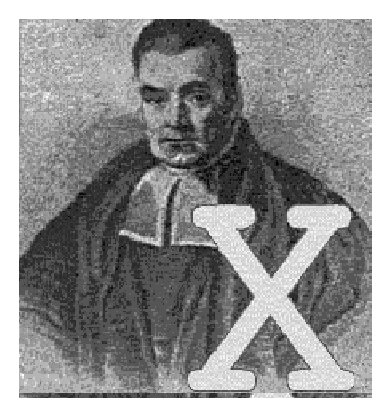
\includegraphics[scale=1.2]{grafiken/bayesicon.eps}
\end{center}
\end{figure}

\vfill

{\bf\sffamily \huge #1}

\vfill

\end{center}

{\em Developed by}

Christiane Belitz\\
Andreas Brezger\\
Nadja Klein (University of G\"{o}ttingen)\\
Thomas Kneib (University of G\"{o}ttingen)\\
Stefan Lang (University of Innsbruck) \\
Nikolaus Umlauf (University of Innsbruck) \\

\vspace{2ex}

{\em With contributions by}

\vspace{-1.5ex}

\begin{multicols}{2}
Daniel Adler\\
Paul Cochrane\\
Jan Fahrenholz\\
Eva-Maria Fronk\\
Felix Heinzl\\
Andrea Hennerfeind\\
Manuela Hummel\\
Alexander Jerak\\
Susanne Konrath\\
Petra Kragler\\
Cornelia Oberhauser\\
Leyre Est\'{\i}baliz Osuna Echavarr\'{\i}a\\
Daniel Saban\'{e}s Bov\'{e} \\
Achim Zeileis
\end{multicols}

{\em Supported by}

Ludwig Fahrmeir (mentally)\\
Leo Held (mentally)\\
German Research Foundation (DFG)

\newpage

\subsection*{Acknowledgements}

The development of {\em BayesX} has been supported by grants from the German Research Foundation (DFG), Collaborative
Research Center 386 ``Statistical Analysis of Discrete Structures''.

Special thanks go to (in alphabetical order of first names):

{\em Dieter Gollnow} for computing and providing the map of Munich (a really hard job); \\
{\em Leo Held} for advertising the program; \\
{\em Ludwig Fahrmeir} for his patience with finishing the program and for carefully
reading and correcting the  manual; \\
{\em Ngianga-Bakwin Kandala} for being the first user of the program (a really hard job); \\
{\em Samson Babatunde Adebayo} for carefully reading and correcting the manual; \\
{\em Ursula Becker} for carefully reading and correcting the manual;

\subsection*{Licensing agreement}

This program is free software; you can redistribute it and/or
modify it under the terms of the GNU General Public License
as published by the Free Software Foundation; either version 2
of the License, or (at your option) any later version.

This program is distributed in the hope that it will be useful,
but WITHOUT ANY WARRANTY; without even the implied warranty of
MERCHANTABILITY or FITNESS FOR A PARTICULAR PURPOSE.  See the
GNU General Public License for more details.

You should have received a copy of the GNU General Public License
along with this program; if not, write to the Free Software
Foundation, Inc., 51 Franklin Street, Fifth Floor, Boston, MA  02110-1301, USA.



\vspace{0.5cm}

{\em BayesX} is available at { \href{http://www.bayesx.org}{http://www.bayesx.org}}}


 \externaldocument{manual}
 \externaldocument{manual_tutorials}

 \makeindex

\begin{document}
\MakeShortVerb{\#}

\preface{Methodology Manual}

\newpage

\section{Introduction}

In this manual we provide a brief review of the methodological background for the four regression tools currently implemented
in {\em BayesX}. The first two regression tools ({\em bayesreg objects} and {\em mcmcreg objects}) rely on Markov chain Monte Carlo (MCMC) simulation
techniques and yields fully Bayesian posterior mean or posterior mode estimates. While {\em bayesreg objects} provide access to exponential family structured additive regression as well as survival times and multi-state models, {\em mcmcreg objects} implement distributional and quantile structured additive regression models as well as multilevel extensions of structure additive regression.
The third regression tool ({\em remlreg objects}) is based on the mixed model representation of penalised regression models with inference being based on penalised
maximum likelihood and marginal likelihood (a generalisation of restricted maximum likelihood) estimation. The fourth regression
tool ({\em stepwisereg objects}) simultaneously performs model choice and estimation with inference being based on penalised
likelihood. MCMC techniques are partly used for computing interval estimates. All regression tools allow to estimate structured
additive regression (STAR) models (\citeasnoun{BelLan08}, \citeasnoun{BreLan06}, \citeasnoun{FahKneLan04}) with complex semiparametric predictors.
STAR models cover a number of well
known model classes as special cases, including {\em generalized additive models} \cite{HasTib90}, {\em generalized additive
mixed models} \cite{LinZha99}, {\em geoadditive models} \cite{KamWan03}, {\em varying coefficient models} \cite{HasTib93}, and
{\em geographically weighted regression} \citeasnoun{FotBruCha02}. Besides models for responses from univariate exponential
families, BayesX also supports non-standard regression situations such as models for categorical responses with either ordered
or unordered categories, uni- and multivariate distributional regression in the spirit of generalised additive models for location, scale and shape with parametric response distributions beyond the exponential family framework, Bayesian quantile regression, continuous time survival data, or continuous time multi-state models. To provide a first impression of
structured additive regression, Sections~\ref{obsmodel} to \ref{inference} describe STAR models for exponential family
regression. Section~\ref{survivalAnalysis} extends structured additive regression to the analysis of survival times and
multi-state data while Section~\ref{distreg_star} considers extensions for distributional regression, quantile regression and multilevel specifications. Full details on STAR methodology can be found in the following references:

\subsubsection*{Structured additive regression based on MCMC
simulation}

\begin{itemize}
\item Brezger, A., Lang, S. (2006): Generalized Structured Additive Regression based on Bayesian P-Splines. {\it
    Computational Statistics and Data Analysis}, {\bf 50}, 967--991.
    \vspace{-0.25cm}
\item Brezger, A., Lang, S. (2008)
      Simultaneous Probability Statements for Bayesian P-splines.
      {\it Statistical Modelling}, {\bf 8},
      141--168.\vspace{-0.25cm}
\item Brezger, A., Steiner, W. (2008): Monotonic Regression based on Bayesian P-Splines: an Application to Estimating Price Response Functions from Store-level Scanner Data. {\it Journal of Economic and Business Statistics}, {\bf 26}, 90--104. \vspace{-0.25cm}
\item Fahrmeir, L.,  Kneib, T., Lang, S., Marx, B. (2013):
{\it Regression: Models, Methods and Applications},
 New York: Springer-Verlag.\vspace{-0.25cm}
 \item Fahrmeir, L., Lang, S. (2001): Bayesian Inference for Generalized Additive Mixed Models based on Markov Random Field
    Priors. {\it Journal of the Royal Statistical Society C (Applied Statistics)}, {\bf 50}, 201--220.\vspace{-0.25cm}
\item Fahrmeir, L., Lang, S. (2001): Bayesian Semiparametric Regression Analysis of Multicategorical Time-Space Data. {\it
    Annals of the Institute of Statistical Mathematics}, {\bf 53}, 10--30.\vspace{-0.25cm}
\item Fahrmeir, L., Osuna, L.. (2006): Structured Additive Regression for Overdispersed and Zero-Inflated Count Data. {\it
    Applied Stochastic Models in Business and Industry}, {\bf 22}, 351--369.\vspace{-0.25cm}
\item Hennerfeind, A., Brezger, A., Fahrmeir, L. (2006): Geoadditive Survival Models. {\it Journal of the American
    Statistical Association}, {\bf 101}, 1065--1075.\vspace{-0.25cm}
\item Klein, N., Kneib, T., Lang, S. (2013): Bayesian Structured Additive Distributional Regression.  Under revision for {\it Annals of Applied Statistics}.\vspace{-0.25cm}
\item Klein, N., Kneib, T., Lang, S. (2014): Bayesian Generalized Additive Models for Location, Scale and Shape for Zero-Inflated and Overdispersed Count Data. To appear in {\it Journal of the American Statistical Association}, doi:10.1080/01621459.2014.912955.\vspace{-0.25cm}
\item Klein, N., Kneib, T., Klasen, S., Lang, S.(2014): Bayesian Structured Additive Distributional Regression for Multivariate Responses. To appear in {\it Journal of the Royal Statistical Society C}, doi:10.1111/rssc.12090.\vspace{-0.25cm}
\item Kneib, T., Hennerfeind, A. (2006) Bayesian Semiparametric Multi-State Models. {\it Statistical Modelling}, {\bf 8},
    169--198..\vspace{-0.25cm}
\item Lang, S., Brezger, A. (2004): Bayesian P-Splines {\it Journal of Computational and Graphical Statistics}, {\bf 13},
    183--212.\vspace{-0.25cm}
\item Lang, S., Umlauf, N., Wechselberger, P., Harttgen, K. and Kneib, T. (2014): Multilevel Structured Additive Regression, {\it Statistics and Computing}, {\bf 24}, 223--238
\end{itemize}

Presumably the best starting point is the paper by \citeasnoun{BreLan06} or the monograph by Fahrmeir et al. (2013).

\begin{figure}[ht]
\footnotesize
\begin{center}
%\begin{tabular}{|p{8cm}|p{5cm}|}
%\hline
%{\bf Intended use} & {\bf recommended sections } \\
%\hline
%semiparametric regression, fully Bayesian approach  & sections \ref{obsmodel}, \ref{priorassumptions} , \ref{fullbayes} \\
%\hline
%semiparametric regression, inference based on mixed model technology, classical perspective &
%sections \ref{obsmodel}, \ref{penalizedleastsquares}, \ref{glmmrep}, \ref{glmmmeth} \\
%\hline
%semiparametric regression, inference based on mixed model technology, Bayesian point of view & sections \ref{obsmodel}, \ref{priorassumptions},
%\ref{glmmrep}, \ref{glmmmeth} \\
%\hline
%semiparametric regression including model choice & sections \ref{obsmodel}, \ref{penalizedleastsquares}, \ref{stepwiseest} \\
%\hline
%\end{tabular}
% \vspace{3mm}
\[\mbox{
 \beginpicture
 \setcoordinatesystem units <1.0cm,1.0cm> point at 0 0
 \setlength{\unitlength}{1.0cm}

 \put {\framebox(5.5,0.7){\sffamily\bfseries 2 Generalized regression models}} at 0 0

 \put {Bayesian perspective} at -4 -1.2
 \put {frequentist perspective} at 4 -1.2

 \arrow <4mm> [0.25,0.75] <0pt,5mm> from 0 -1 to -5 -2.9
 \arrow <4mm> [0.25,0.75] <0pt,5mm> from 0 -1 to 5 -2.9

 \put {\framebox(4.5,0.7){\sffamily\bfseries 4 Bayesian point of view}} at -5 -3

 \put {\framebox(4.5,0.7){\sffamily\bfseries 3 Penalised likelihood}} at 5 -3

 \arrow <4mm> [0.25,0.75] <0pt,5mm> from -5 -4 to 0 -6
 \arrow <4mm> [0.25,0.75] <0pt,5mm> from 5 -4 to 0 -6

 \put {relation to mixed models} at 0 -4.5

 \put {\framebox(5.5,0.7){\sffamily\bfseries 5 Mixed model representation}} at 0 -6

 \arrow <4mm> [0.25,0.75] <0pt,5mm> from -5 -4 to -5 -13
 \arrow <4mm> [0.25,0.75] <0pt,5mm> from -5 -8 to 0 -13
 \arrow <4mm> [0.25,0.75] <0pt,5mm> from 5 -4 to 5 -9

 \put {\framebox(3.5,0.7){\sffamily\bfseries 6.1 bayesreg object}} at -5 -13
 \put {\framebox(3.5,0.7){\sffamily\bfseries 6.3 stepwisereg objects}} at 5 -9

 \put {MCMC (full Bayes)} at -6.5 -6
 \put {penalised likelihood} at 6.5 -5.75
 \put {incl. model choice} at 6.4 -6.25

 \arrow <4mm> [0.25,0.75] <0pt,5mm> from 0 -7 to 0 -9

 \put {penalised likelihood} at -1.5 -7.5
 \put {(empirical Bayes)} at 1.3 -7.5

 \put {\framebox(3.5,0.7){\sffamily\bfseries 6.2 remlreg objects}} at 0 -9
 \put {\framebox(3.5,0.7){\sffamily\bfseries 8 mcmcreg objects}} at 0 -13

 \put {exponential family} at -6.4 -10
 \put {durations} at -5.8 -10.5
 \put {categorical responses} at -6.6 -11

 \put {distributional regression} at -0.6 -10
 \put {quantile regression} at -0.4 -10.5
 \put {multilevel models} at 0.1 -11

 \endpicture
}\]
 \vspace{3mm}

{\em \caption {\label{guideline} Guidelines for reading this
manual.}}
\end{center}
\end{figure}

\subsubsection*{Structured additive regression based on mixed model
methodology}

\begin{itemize}
\item Fahrmeir, L., Kneib, T., Lang, S. (2004): Penalized Structured Additive Regression for Space-Time Data: a Bayesian
    Perspective. {\it Statistica Sinica}, {\bf 14}, 715--745.\vspace{-0.25cm}
\item Kneib, T. (2006): Mixed Model based Inference in Structured Additive Regression. Dr. Hut Verlag, M\"{u}nchen. Available
    online from
    \href{http://edoc.ub.uni-muenchen.de/archive/00005011/}{http://edoc.ub.uni-muenchen.de/archive/00005011/}\vspace{-0.25cm}
\item Kneib, T. (2006): Geoadditive Hazard Regression for Interval Censored Survival Times. {\it Computational Statistics
    and Data Analysis}, {\bf 51}, 777--792.\vspace{-0.25cm}
\item Kneib, T., Fahrmeir, L. (2007): A Mixed Model Approach for Geoadditive Hazard Regression. {\it Scandinavian Journal
    of Statistics}, {\bf 34}, 207--228.\vspace{-0.25cm}
\item Kneib, T., Fahrmeir, L. (2006): Structured Additive Regression for Multicategorical Space-Time Data: A Mixed Model
    Approach. {\it Biometrics}, {\bf 62}, 109--118.\vspace{-0.25cm}
\item Kneib, T., Hennerfeind, A. (2006): Bayesian Semiparametric Multi-State Models. {\it Statistical Modelling}, {\bf 8},
    169--198.
\end{itemize}

Presumably the best starting point is the paper by \citeasnoun{FahKneLan04} or the monograph by \citeasnoun{Kne06}.

\subsubsection*{Structured additive regression including model selection}

\begin{itemize}
\item Belitz, C. (2007): Model Selection in Generalised Structured Additive Regression Models. Dr. Hut Verlag, M\"{u}nchen.
\item Belitz, C., Lang, S. (2008) Simultaneous Selection of Variables and Smoothing Parameters
in Structured Additive Regression Models. {\it
Computational Statistics and Data Analysis}, {\bf 53} , 61-81.
\end{itemize}

Presumably the best starting point is the paper by \citeasnoun{BelLan08}.

\subsubsection*{Guideline for the reader}


The rest of this manual is organized as follows:

The next section describes the general structure of STAR models for
distributions of the response variable belonging to an exponential
family. The following Sections~\ref{penalizedleastsquares} --
\ref{inference} discuss alternative approaches for specifying and
estimating the different model terms in STAR models. Section
\ref{penalizedleastsquares} describes the models from a more
classical penalized least squares perspectives. A Bayesian point of
view is taken in Section \ref{priorassumptions}. The close
connection to mixed models is highlighted in Section \ref{glmmrep}.
Section \ref{inference} gives a brief outline of the various
inference techniques for exponential family STAR models. Fully Bayesian inference via
MCMC simulation techniques for exponential family responses, categorical responses and duration times is the topic of Section \ref{fullbayes}.
Inference based on mixed model technology is sketched in Section
\ref{glmmmeth}. Simultaneous selection of relevant model terms and
estimation of the parameters is described in Section
\ref{stepwiseest}. Section~\ref{survivalAnalysis} discusses extensions for duration times and multi-state models while Section~\ref{distreg_star} provides details on distributional regression, quantile regression and multilevel specifications.

For most users of BayesX it is sufficient to read only parts of this
manual. Some recommendations are given in Figure \ref{guideline}.


\section{Generalized regression models}
\label{obsmodel}

\index{Generalized linear model}\index{Exponential family}
Generalized linear models assume that, given covariates $\uvec$ and
unknown parameters $\gammavec$, the distribution of the response
variable $y$ belongs to an exponential family, i.e.
\begin{equation}
\label{likel} p(y \, | \, \uvec) = \exp \left( \frac{y \theta -
b(\theta)}{\phi} \right) c(y,\phi)
\end{equation}
where $b(\cdot)$, $c(\cdot)$, $\theta$ and $\phi$ determine the specific response distribution. A list of the most common
distributions and their parameters can be found for example in \citeasnoun{FahTut01}, page 21. The mean
$\mu=E(y|\uvec,\gammavec)$ is linked to a linear predictor $\eta$ by
\begin{equation}
\label{glm} \mu=h(\eta) \qquad \eta= \uvec'\gammavec,
\end{equation}
where $h$ is a known response function and $\gammavec$ are unknown
regression parameters.

In most practical regression situations, however, we are facing at
least one of the following problems:
\begin{itemize}
\item For the {\em continuous covariates} in the data set, the assumption of a strictly linear
effect on the predictor may be not appropriate. \vspace{-0.2cm}
\item Observations may be {\em spatially correlated}.
\vspace{-0.2cm}
\item Observations may be {\em temporally correlated}.
\vspace{-0.2cm}
\item Complex interactions may be required to model the joint effect
of some of the covariates adequately. \vspace{-0.2cm}
\item  Heterogeneity among individuals or units may be not sufficiently described by covariates. Hence,
unobserved {\em unit or cluster specific heterogeneity} has to be
considered appropriately.
\end{itemize}
To overcome these difficulties, we replace the strictly linear
predictor in (\ref{glm}) by a structured additive predictor
\begin{equation}
\label{gampred} \eta=f_{1}(x_{1})+\ldots+f_j(x_j) +
\ldots+f_{p}(x_{p})+\uvec'\gammavec,
\end{equation}
where $x_j$ denote
covariates of different type and dimension, and $f_j$ are (not
necessarily smooth) functions of the covariates. The functions $f_j$
comprise usual nonlinear effects of continuous covariates, time
trends and seasonal effects, two-dimensional surfaces, varying
coefficient models, i.i.d. random intercepts and slopes as well as
spatial effects. STAR-models cover a number of special cases
well known from the literature, in particular {\em Generalized additive models (GAM)},
{\em Generalized additive mixed models (GAM)}, {\em Geoadditive models}, {\em Multilevel models},
{\em Varying coefficient models (VCM)}, {\em ANOVA type interaction models} and {\em geographically weighted regression}.

\section{Penalized least squares}
\label{penalizedleastsquares}

In BayesX, the nonlinear functions $f_j$ are modeled by a basis
functions approach, i.e. a particular nonlinear function $f$ is
approximated by a linear combination of basis functions:
$$
f(x) = \sum_{k=1}^{K} \beta_k B_k(x)
$$
The $B_k$ are known basis functions and $\betavec =
(\beta_1,\dots,\beta_K)'$ is a vector of unknown regression
coefficients to be estimated. Note that the term basis function in
our understanding is not limited to basis functions known from
nonparametric smoothing such as B-splines but also refers to
non-standard basis functions such as indicator functions for regions
or clusters. To ensure enough flexibility, typically a large number
of basis functions is defined. To avoid overfitting, a roughness
penalty on the regression coefficients is additionally specified. We
use quadratic penalties of the form $\betavec' \Pvec(\lambdavec)
\betavec$ where $\Pvec(\lambdavec)$ is a penalty matrix. The penalty
depends on one or multiple smoothing parameters $\lambdavec$ that
govern the amount of smoothness imposed on the function $f$. Most
penalty matrices are of the particular simple form
$\Pvec(\lambdavec) = \lambda \Kvec$ where $\lambda$ is a scalar
smoothing parameter. For {\em stepwisereg objects} more complicated
penalties are sometimes possible. They are an additive combination
of penalty matrices. An example is $\Pvec(\lambdavec) = \lambda_1
\Kvec_1+\lambda_2 \Kvec_2$ where $\lambda_1$ and $\lambda_2$ are
smoothing parameters and $\Kvec_1$ and $\Kvec_2$ are penalty
matrices.

The choice of basis functions $B_1,\dots,B_K$ and penalty  $\Pvec(\lambdavec)$ depends on our prior assumptions about the smoothness
of $f$ as well as
the type and dimension of $x$. We will give specific examples below. Defining the $n \times K$ design matrix $\Xvec$ with elements
$X[i,k] = B_k(x_i)$ the
vector $\fvec = (f(x_1),\dots,f(x_n))'$ of function evaluations can be written in matrix notation as $\fvec = \Xvec \betavec$.
Accordingly,  for model (\ref{gampred}) we obtain
$$
\etavec = \Xvec_1 \betavec_1 + \ldots + \Xvec_p \betavec_p + \Uvec \gammavec +  \varepsilonvec,
$$
where $\Uvec$ is the design matrix for linear effects, $\gammavec$ is the vector of regression coefficients for linear effects, and
$\varepsilonvec$
are the vectors of observations and errors.
In the next subsections we will give specific examples for modeling the unknown functions $f_j$ or in other words for the choice of basis functions and
penalty matrices.
We start with modeling the effect of continuous covariates using splines.

\subsection{Continuous covariates}
\subsubsection{P(enalized)-splines}
Suppose first that a particular component $x$ of the covariate  is univariate and continuous. There is a considerable amount of
literature on basis functions approaches in combination with a (quadratic) roughness penalty for continuous covariates. BayesX
applies the P-splines approach introduced by \citeasnoun{EilMar96}. The approach assumes that the unknown functions can be
approximated by a polynomial spline of degree $l$ and with equally spaced knots
$$
x_{min} = \zeta_{0}  < \zeta_{1} < \dots < \zeta_{m-1} < \zeta_{m} = x_{max}
$$
over the domain of $x$. The spline can be written in terms of a linear combination of $K=m+l$ B-spline basis functions. The
columns of the design matrix $\Xvec$ are given by the B-spline basis functions evaluated at the observations $x_i$. To overcome
the well known difficulties involved with regression splines, \citeasnoun{EilMar96} suggest a relatively large number of knots
(usually between 20 to 40) to ensure enough flexibility, and to introduce a roughness penalty on adjacent regression
coefficients based on squared $r$-th order differences, i.e.
$$
\betavec' \lambda \Kvec \betavec = \lambda \sum_{k=r+1}^K (\Delta^r \beta_k)^2.
$$
The penalty matrix is given by $\Kvec =  \Dvec_r' \Dvec_r$ where $\Dvec_r$ is a $r$-th order difference matrix.
Typically, second or third order differences are used. The limiting behavior $\lambda \rightarrow \infty$ depends both on the
order of the spline
and the order of the penalty. If the order of the spline is equal to or
higher than the order of  the penalty, which is typically the case, then a polynomial
fit of degree $r-1$ is obtained in the limit.

The approach can be extended to impose monotonicity or more general shape constraints. We follow an approach proposed by
\citeasnoun{BolEilvMe06}. A sufficient condition for a decreasing spline is given by $\beta_{k} \leq \beta_{k-1}$, i.e.  a
parameter $\beta_{k}$ is less than its predecessor $\beta_{k-1}$. The simple but powerful idea  is to impose the required
constraint by expanding the penalty by an additional  term. More specifically they propose the composed penalty
$$
\Pvec(\lambdavec) =  \betavec' \left( \lambda_1 \Kvec_1 + \lambda_2 \Kvec_2 \right) \betavec
$$
where $\lambda_1$ and $\Kvec_1$ are the usual smoothing parameter
and penalty matrix for P-splines. The additional penalty matrix
$\Kvec_2$ is a diagonal matrix with entries 1 whenever the condition
$\beta_{k} \leq \beta_{k-1}$ fails and 0 otherwise. For increasing
functions, $\Kvec_2$ has to be adapted accordingly. The parameter
$\lambda_2$ is not estimated but set large enough to enforce
monotonic functions.





\subsubsection{Tensor product P-splines}
\label{tensorproductpsplines} Assume now that $\xvec$ is
two-dimensional, i.e. $\xvec = \left(x^{(1)},x^{(2)}\right)'$ with
continuous components $x^{(1)}$ and $x^{(2)}$. The aim is to extend
the univariate P-spline from the preceding section to two
dimensions. A common approach is to approximate the unknown surface
$f(x)$ by the tensor product of one dimensional B-splines, i.e.
\begin{equation}
\label{gampspline_2dimterm} f\left(x^{(1)},x^{(2)}\right) = \sum_{k=1}^{K_1}
\sum_{s=1}^{K_2} \beta_{ks} B_{1,k}(x^{(1)})
B_{2,s} (x^{(2)}),
\end{equation}
where $B_{11},\dots,B_{1K_1}$ are the basis functions in $x^{(1)}$ direction and
$B_{21},\dots,B_{2K_2}$ in $x^{(2)}$ direction.
The $n \times K = n \times K_1 K_2$ design matrix $\Xvec$ now consists of
products of basis functions.

Several alternatives are available for the penalty matrix $\Pvec(\lambdavec)$:
\begin{enumerate}
\item[a)] {\em Penalty based on first differences:} The
two-dimensional generalization of a penalty based on first
differences is given by combining row- and column wise quadratic
differences
$$
\begin{array}{l}
\displaystyle \sum_{k=2}^{K_1}\sum_{s=1}^{K_2}(\beta_{ks}-\beta_{k-1,s})^2 =
\betavec'(\Ivec_{K_2}\otimes \Dvec_1)'(\Ivec_{K_2}\otimes \Dvec_1)\betavec \\[0.4cm]
\displaystyle  \sum_{k=1}^{K_1}\sum_{s=2}^{K_2}(\beta_{ks}-\beta_{k,s-1})^2 =
\betavec'(\Dvec_2\otimes \Ivec_{K_1})'(\Dvec_2\otimes \Ivec_{K_1})\betavec \\
\end{array}
$$
to the penalty
$$
\betavec'\Pvec(\lambdavec) \betavec =  \betavec' \lambda \left[ (\Ivec_{K_2}\otimes \Dvec_1)'(\Ivec_{K_2}\otimes \Dvec_1) + (\Dvec_2\otimes \Ivec_{K_1})'
(\Dvec_2\otimes \Ivec_{K_1})\right]\betavec.
$$
Another way of expressing the penalty is given by
\begin{equation}
\label{2dpenalty}
 \betavec'\Pvec(\lambda)\betavec = \betavec'\lambda \left[\Ivec_{K_2}\otimes\Kvec_1 + \Kvec_2\otimes \Ivec_{K_1}\right]\betavec,
\end{equation}
where $\Kvec_1$ and $\Kvec_2$ are the respective one dimensional penalty matrices.
In the limit  $\lambda \rightarrow \infty$ a constant fit is obtained.
\item[b)] {\em Penalty based on second differences:} In a similar way two-dimensional penalties based on higher order differences
are constructed. A second order difference penalty is obtained if
$\Kvec_1$ and $\Kvec_2$ in (\ref{2dpenalty}) correspond to penalty
matrices based on second rather than first differences. Similar to
one dimensional P-splines the limit $\lambda \rightarrow \infty$
results in linear effects in $x^{(1)}$ and $x^{(2)}$ with an
additional interaction effect, i.e.
$$
f\left(z^{(1)},z^{(2)}\right) = c_0 + c_1 \, x^{(1)} + c_2 \,
x^{(2)} + c_3 \, x^{(1)} x^{(2)}.
$$
\item[c)] {\em Anisotropic penalty:} The two penalties considered so far are not capable of
different penalization in $x^{(1)}$ and $x^{(2)}$ direction,
respectively. Anisotropic penalties are obtained by assuming
separate smoothing parameters $\lambda_1$ and $\lambda_2$ in
$x^{(1)}$ and $x^{(2)}$ direction. The penalty is then given by
\begin{equation}
\label{penalty_eilmar}
 \betavec'\Pvec(\lambdavec) \betavec = \betavec'\left[\lambda_1 \Ivec_{K_2}\otimes\Kvec_1 + \lambda_2 \Kvec_2\otimes \Ivec_{K_1}\right]\betavec.
\end{equation}
The resulting fit in the limit $\lambda_1 \rightarrow \infty$ and
$\lambda_2 \rightarrow \infty$ depends on the penalty used to
construct $\Kvec_1$ and $\Kvec_2$. If $\Kvec_1$ and $\Kvec_2$
correspond to a first order difference penalty a constant fit is
obtained in the limit. Second order difference penalties result in a
linear fit for $f\left(x^{(1)},x^{(2)}\right)$.
\item[d)] {\em Penalties with main effects in the limit:} Sometimes it is desirable to decompose the effect of the two covariates
$x^{(1)}$ and $x^{(2)}$ into two main effects modeled by one
dimensional functions and a two-dimensional interaction effect, i.e.
\begin{equation}
\label{pspline_2dimtermmain} f \left(x^{(1)},x^{(2)}\right) =
f_1\left(x^{(1)} \right) + f_2 \left(x^{(2)}\right) + f_{1|2}\left(
x^{(1)},x^{(2)} \right).
\end{equation}
Usually a two-dimensional surface smoother  together with two
additional  one dimensional P-splines (or other smoothers) are
estimated. This approach is possible with {\em bayesreg objects} and
{\em remlreg objects}. {\em stepwisereg objects} take, however, a
different approach. We specify a two-dimensional surface based on
tensor product P-splines and compute the decomposition of the
resulting surface into main effects and the interaction effect {\em
after} estimation. Moreover, we specify a penalty that allows for a
main effects only model as a special case. This allows to
discriminate between a simple  main effects model and a more
complicated two way interactions model. A penalty that guarantees  a
main effects model in the limit is defined by the Kronecker product
of the two penalty matrices for one dimensional P-splines, i.e.
\begin{equation}
\label{penalty_kronecker}
\betavec'\Pvec(\lambda)\betavec = \betavec' \lambda \Kvec_1 \otimes \Kvec_2 \betavec.
\end{equation}
The drawback of this penalty is that the limit $\lambda \rightarrow \infty $ yields {\em unpenalized} main effects, i.e. wiggly functions.
We therefore use a modified penalty which is effectively a combination of the two  penalties  (\ref{penalty_eilmar}) and
(\ref{penalty_kronecker}). More specifically
we define
\begin{equation}
\label{penalty_comb}
\betavec'\Pvec(\lambdavec)\betavec = \betavec' \left[\frac{\lambda_1}{K_1}
\Ivec_{K_2}\otimes\Kvec_1 + \frac{\lambda_2}{K_2} \Kvec_2\otimes \Ivec_{K_1}+\lambda_3 \Kvec_1 \otimes \Kvec_2   \right] \betavec,
\end{equation}
where $\Kvec_1$ and $\Kvec_2$ are penalty matrices corresponding to one dimensional P-splines based on first or second order differences.
This penalty has the following nice properties:
\begin{itemize}
\item The limit $\lambda_3 \rightarrow \infty$ results in a mere main effects model. The main effects  are one dimensional P-splines with smoothing
parameters $\lambda_1$ and $\lambda_2$.
\item The limit $\lambda_3 \rightarrow 0$ yields the anisotropic penalty (\ref{penalty_eilmar}) as a special case.
\item The limit $\lambda_1 \rightarrow 0$ and $\lambda_2 \rightarrow 0$  yields the Kronecker product penalty
(\ref{penalty_kronecker}) as a special case.
\item The limit $\lambda_1 \rightarrow \infty$, $\lambda_2 \rightarrow \infty$ and $\lambda_3 \rightarrow \infty$ results in a main effects model with
linear or constant main effects depending on the difference order used to construct $\Kvec_1$ and $\Kvec_2$.
\end{itemize}
\end{enumerate}


\subsection{Spatial effects}

In this subsection we assume that $x$ represents the location a
particular observation pertains to. The location is typically given
in two ways. If exact locations are available $x=(x^{(1)},x^{(2)})'$
is two-dimensional and the components  $x^{(1)}$ and $x^{(2)}$
correspond to the coordinates of the location. In this case, the
spatial effect $f(x^{(1)},x^{(2)})$ could be modeled by
two-dimensional surface estimators as described in the preceding
section.

In many applications, however, exact locations are not available. Typically, a geographical map is available and $x \in \{1,\dots,K\}$ is an
index that denotes the region (e.g. district) an observation pertains to. A common approach is to assume $f(x) = \beta_x$,
i.e. separate parameters $\beta_1,\ldots,\beta_K$  for each region are estimated.
The $n \times K$ design matrix $\Xvec$ is an incidence matrix whose entry in
the $i$-th row and $k$-th column is equal to one if observation $i$ has been observed at
location $k$ and zero otherwise. To prevent overfitting a penalty based on squared differences is defined that
guarantees that parameters of neighboring regions are similar. Typically two regions are assumed to be neighbors if they share a common
boundary although other neighborhood definitions are possible. The penalty is defined as
$$
\betavec' \lambda \Kvec \betavec = \lambda\sum_{k=2}^{K}\sum_{s \in N(k), s < k}(\beta_k-\beta_s)^2,
$$
where $N(k)$ denotes all sites that are neighbors of site $k$.
The elements of the penalty matrix are given by
\begin{equation}
\label{K_mrf}
 \Kvec[s,r] = \lambda \left\{
 \begin{array}{ll}
-1 & k\neq s, k\sim s,\\
 0 & k\neq s, k \nsim s,\\
 |N(k)| & k=s.
\end{array}
\right.
\end{equation}

Depending on the prior belief on smoothness of the spatial effect
several alternatives to penalty (\ref{K_mrf}) are available. If a
very smooth effect is assumed, the two-dimensional smoothers
discussed in the preceding section could be used as an alternative.
Since exact locations are not available the centroids of the regions
could be used instead.

\subsection{Unit- or cluster specific heterogeneity}
Typically, unit- or cluster specific random effects are introduced
to account for unobserved heterogeneity. In its simplest form, a
random intercept $\beta_x$ with $\beta_x \sim N(0,\tau^2)$ is
introduced. Here, $x \in \{1,\dots,K\}$ is an index variable that
denotes the cluster a particular observation pertains to. This is
equivalent to a penalized least squares approach with function $f(x)
= \beta_x$, penalty matrix $\Ivec$ and smoothing parameter $\lambda
= \sigma^2/\tau^2$. The $n \times K$ design matrix $\Xvec$ is a 0/1
incidence matrix whose entry in the $i$-th row and $k$-th column is
equal to one if observation $i$ belongs to the $k$-th cluster and
zero otherwise. Random slopes could be treated in the same way, see
the next subsection.

A particular cluster variable is a spatial index that indicates the region an observation pertains to. Usually a spatially correlated effect
as described in the preceding subsection is specified.
However, in some situations a smooth spatial effect is not justified because of local, spatial heterogeneity. In this case,
the assumption of spatial dependence of neighboring parameters is not meaningful. Instead, the simple (ridge type) penalty
$$
\betavec' \lambda \Kvec \betavec = \lambda \betavec'  \betavec = \lambda \sum_{k=1}^{K} \beta_k^2
$$
with penalty matrix $\Kvec = \Ivec$ may be defined. This penalty does not assume any spatial dependence but prevents highly variable
estimates induced by small samples for some regions or sites.

Note that more than one random intercept with respect to different
cluster variables are possible. In many cases there exists a
hierarchical ordering of clusters. Models with such hierarchical
clusters are also called multilevel models.


\subsection{Varying coefficients}
\label{varcoeff_terms}

Suppose now that the effect of a continuous covariate $x^{(2)}$ is assumed to vary with
respect to a categorical covariate $x^{(1)}$. For notational convenience, we restrict the discussion to binary covariates $x^{(1)}$.
The generalization to (multi)categorical covariates is straightforward.
The interaction between $x^{(2)}$ and
$x^{(1)}$ can be modeled by a predictor of the form
$$
\eta = \ldots + f_1(x^{(2)}) + g(x^{(2)}) x^{(1)} + \ldots,
$$
where $f_1$ and $g$ are smooth functions (modeled by P-splines). The
interpretation of the two functions $f_1$ and $g$ depends on the
coding of the binary variable $x^{(1)}$. If $x^{(1)}$ is in
dummy-coding, the function $f_1$ corresponds to the effect of
$x^{(2)}$ subject to  $x^{(1)}=0$, and $g$ is the difference effect
for observations with $x^{(1)}=1$. If $x^{(1)}$ is in effect-coding,
the function $f_1$ can be interpreted as an average effect of
$x^{(2)}$, where $g$ and $-g$ represent the deviation from $f_1$ for
$x^{(1)} = 1$ and $x^{(1)} = -1$, respectively. It turns out that
the coding of $x^{(2)}$ is not only important  for interpretation
but sometimes also crucial for inference (in {\em bayesreg objects}
and {\em stepwisereg objects}). Estimation for {\em bayesreg and
stepwisereg objects} described in the next section is based on an
iterative backfitting type procedure. Hence dependence between $f_1$
and $g$ should be minimized to avoid convergence problems. Hence,
effect coding for $x^{(2)}$ is an effective yet simple device to
avoid convergence problems.

Models with interaction effects of the form $g(x^{(2)}) \, x^{(1)}$ are  known as varying coefficient models  because the
effect of $x^{(1)}$ varies smoothly with respect to the continuous covariate $x^{(2)}$. Covariate $x^{(2)}$ is called the
effect modifier of $x^{(1)}$. The approach can be easily extended to a two-dimensional effect modifier with components
$x^{(2)}$ and $x^{(3)}$. The interaction effect is then given by $g(x^{(2)},x^{(3)}) \, x^{(1)}$ where $g(x^{(2)},x^{(3)})$ is
a two-dimensional surface which is modeled by the tensor product P-splines discussed in section \ref{tensorproductpsplines}.
Another modification arises if the effect modifier is the location either given as the coordinates or as a spatial index. In
this case we have a space varying effect of $x^{(1)}$. Models of this kind are also known as geographically weighted
regression, see \citeasnoun{FotBruCha02}. A final modification is obtained for a unit or cluster index as effect modifier. The
effect of $x^{(1)}$ is now assumed to be unit- or cluster-specific and typically referred to as a random slope.

Independent of the specific type of the effect modifier, the interaction term $g\left(x^{(2)}\right) \, x^{(1)}$
(or $g\left(x^{(2)},x^{(3)}\right) \, x^{(1)}$) can be cast into our
general framework by defining
\begin{equation}
\label{gampspline_varcoeffterm}
f\left(x^{(1)},x^{(2)}\right) = g\left(x^{(2)}\right) \, x^{(1)} \quad \mbox{or} \quad  f\left(x^{(1)},x^{(2)},x^{(3)}\right) =
g\left(x^{(2)},x^{(3)}\right) \, x^{(1)}.
\end{equation}
The overall design matrix $\Xvec$ is given by
$\diag(x_{1}^{(1)},\dots,x_{n}^{(1)}) \, \Xvec^{(1)}$ where
$\Xvec^{(1)}$ is the usual design matrix for P-Splines, tensor
product P-splines, spatial-, or cluster-specific effects.



\section{Bayesian point of view}
\label{priorassumptions}\index{Prior assumptions}

For Bayesian inference, the unknown functions $f_{1},\dots ,f_{p}$
in predictor (\ref{gampred}), more exactly corresponding vectors of
function evaluations, and the fixed effects parameters $\gammavec$ are
considered as random variables and must be supplemented by
appropriate prior assumptions.

In the absence of any prior knowledge, diffuse priors are the
appropriate choice for fixed effects parameters, i.e.
$$
 p(\gamma_j) \propto const
$$
Another common choice, not yet supported by {\em BayesX}, are
informative multivariate Gaussian priors with mean $\muvec_0$ and
covariance matrix $\Sigmavec_0$.\index{Prior assumptions!Fixed effects}


Priors for the unknown functions $f_{1},\dots,f_{p}$ depend on the
{\em type of the covariates} and on {\em prior beliefs about the
smoothness of $f_j$.} In the following we express the vector of
function evaluations $\fvec_j=(f_j(x_{1j}),\dots,f_j(x_{nj}))'$ of a
function $f_j$ as the matrix product of a design matrix $\Xvec_j$ and a
vector of unknown parameters $\betavec_j$, i.e.
\begin{equation}
\label{matproduct} \fvec_j=\Xvec_j \betavec_j.
\end{equation}
Then, we obtain the predictor (\ref{gampred}) in matrix notation
as
\begin{equation}
\label{gampredmatrix} \etavec = \Xvec_1 \betavec_1 + \cdots + \Xvec_p \betavec_p +
\Uvec \gammavec,
\end{equation}
where $\Uvec$ corresponds to the usual design matrix for fixed
effects.

A prior for a function $f_j$ is defined by specifying a suitable
design matrix $\Xvec_j$ and a prior distribution for the vector
$\betavec_j$ of unknown parameters. The general form of the prior for
$\betavec_j$ is given by
\begin{equation}
\label{genform} p(\betavec_j | \tau_j^2) \propto
\frac{1}{(\tau^2_j)^{rank(\Kvec_j)/2}} \exp\left(-\frac{1}{2\tau_j^2}
\betavec_j' \Kvec_j \betavec_j\right),
\end{equation}
where $\Kvec_j$ is a {\em penalty matrix}. In most cases $\Kvec_j$ will be
rank deficient and therefore the prior for $\betavec_j$ is partially improper.

The variance parameter $\tau_j^2$ is  equivalent to the inverse
smoothing parameter in a penalized likelihood approach and controls the
trade off between flexibility and smoothness.

In the following we will describe specific priors for different
types of covariates and functions $f_j$.


\subsection{Continuous covariates}
\label{psplines}\index{Continuous covariates}\index{Time scales}
\index{Prior assumptions!Continuous covariates}

Several alternatives have been  proposed for specifying smoothness priors for continuous covariates or time scales. These are
{\em random walk priors} or more generally {\em autoregressive priors} (see \citeasnoun{FahLan01a} and \citeasnoun{FahLan01b},
{\em Bayesian P-splines} \cite{LanBre04} and {\em Bayesian smoothing splines} \cite{HasTib00}. {\em BayesX} supports random
walk priors and P-splines.

\subsubsection{Random walks}\index{Random walk priors}

Suppose first that $x$ is a time scale or continuous covariate
with equally spaced ordered observations
$$
x^{(1)} < x^{(2)} < \cdots < x^{(K)}.
$$
Here $K \leq n$ denotes the number of {\em different} observed
values for $x$ in the data set. A common approach in dynamic or
state space models is to estimate one parameter $\beta_{k}$ for
each distinct $x^{(k)}$, i.e. $f(x^{(k)}) = \beta_{k}$, and
penalize too abrupt jumps between successive parameters using random
walk priors. For example, first and second order random walk models
are given by
\begin{equation}
\label{rwpriors}
\beta_{k}=\beta_{k-1}+u_{k}\,\,\,\,\mbox{and}\,\,\,\,\beta_{k}=2\beta_{k-1}-\beta_{k-2}+u_{k}
\end{equation}
with Gaussian errors $u_{k}\sim N(0,\tau^{2})$ and diffuse priors
$p(\beta_{1})\propto const$, and $p(\beta_{1})$ and
$p(\beta_{2})\propto const$, for initial values, respectively. Both
specifications act as smoothness priors that penalize too rough
functions $f$. A first order random walk penalizes abrupt jumps
$\beta_{k}-\beta_{k-1}$ between successive states while a second
order random walk penalizes deviations from the linear trend $2
\beta_{k-1}-\beta_{k-2}$. The joint distribution of the
regression parameters $\betavec$ is easily computed as the product of
conditional densities defined by (\ref{rwpriors}) and can be brought
into the general form (\ref{genform}). The penalty matrix is of the
form $\Kvec=\Dvec'\Dvec$ where $\Dvec$ is a first or second order difference
matrix. For example, for a random walk of first order the penalty
matrix is given by:
$$
\Kvec = {\footnotesize \left(
\begin{array}{rrrrr}
 1 & -1 & & &  \\
-1 & 2 & -1 & & \\
 &  \ddots & \ddots & \ddots &  \\
 & & -1 & 2 & -1 \\
  & & & -1 & 1
\end{array}
\right) }.
$$
The design matrix $\Xvec$ is a simple 0/1 matrix where the number of
columns equals the number of parameters, i.e. the number of distinct
covariate values. If for the $i$-th observation $x_{i}=x^{(k)}$
the element in the $i$-th row and $k$-th column of $\Xvec$ is one and
zero otherwise.

In case of non-equally spaced observations slight modifications of the priors defined in (\ref{rwpriors}) are necessary, see
\citeasnoun{FahLan01a} for details.

\subsubsection{P-splines}\index{P-splines}

A second approach for effects of continuous covariates, that is closely related to random walk models, is based on P-splines
introduced by \citeasnoun{EilMar96}. The approach assumes that an unknown smooth function $f$ of a covariate $x$ can be
approximated by a polynomial spline of degree $l$ defined by a set of equally spaced knots $x_{min} = \zeta_{0}  < \zeta_{1} <
\dots < \zeta_{m-1} < \zeta_{m} = x_{max}$ within the domain of $x$. Such a spline can be written in terms of a linear
combination of $K = m+l$ B-spline basis functions $B_{k}$, i.e.
$$
f(x) = \sum_{k=1}^{K} \beta_{k} B_{k}(x).
$$
In this case, $\betavec = (\beta_{1},\dots,\beta_{K})'$ corresponds to the vector of unknown regression coefficients and the $n
\times K$ design matrix $\Xvec$ consists of the basis functions evaluated at the observations $x_{i}$, i.e. $\Xvec[i,k] =
B_k(x_{i})$. The crucial point is the choice of the number of knots. For a small number of knots, the resulting spline may not
be flexible enough to capture the variability of the data. For a large number of knots, estimated curves tend to overfit the
data and, as a result, too rough functions are obtained. As a remedy, \citeasnoun{EilMar96} suggest a moderately large number
of equally spaced knots (usually between 20 and 40) to ensure enough flexibility, and to define a roughness penalty based on
first or second order differences of adjacent B-Spline coefficients to guarantee sufficient smoothness of the fitted curves.
This leads to penalized likelihood estimation with penalty terms
\begin{equation}
\label{diffpenalty} \lambda \sum_{k=r+1}^{K}
(\Delta^r \beta_{k})^2 , \quad r=1,2
\end{equation}
where $\lambda$ is the smoothing parameter. First order differences penalize abrupt jumps $\beta_{k}-\beta_{k-1}$ between
successive parameters while second order differences penalize deviations from the linear trend $2 \beta_{k-1}-\beta_{k-2}$. In
a Bayesian approach we use the stochastic analogue of difference penalties, i.e. first or second order random walks, as priors
for the regression coefficients. Note that simple first or second order random walks can be regarded as P-splines of degree
$l=0$ and are therefore included as a special case. More details about Bayesian P-splines can be found in \citeasnoun{LanBre04}
and \citeasnoun{BreLan06}.

\subsubsection{Tensor product P-splines}
\label{tensorproductpsplines_bayes}

Assume now that $x$ is two-dimensional, i.e. $x = \left(x^{(1)},x^{(2)}\right)'$ with continuous components $x^{(1)}$ and
$x^{(2)}$. Similar to section \ref{tensorproductpsplines} the aim is to extend the univariate P-spline to two dimensions. In
{\em BayesX} Bayesian surface fitting is based on two-dimensional P-splines described in more detail in \citeasnoun{LanBre04}
and \citeasnoun{BreLan06}. The unknown surface $f(x^{(1)},x^{(2)})$ is approximated by the tensor product of two
one-dimensional B-splines, i.e.
$$
f\left(x^{(1)},x^{(2)}\right) = \sum_{k=1}^{K_1}
\sum_{s=1}^{K_2} \beta_{ks} B_{1,k}(x^{(1)})
B_{2,s} (x^{(2)}),
$$
where $B_{11},\dots,B_{1K_1}$ are the basis functions in $x^{(1)}$ direction and
$B_{21},\dots,B_{2K_2}$ in $x^{(2)}$ direction.
The $n \times K = n \times K_1 K_2$ design matrix $\Xvec$ now consists of
products of basis functions.

Priors for
$\betavec = (\beta_{11},\dots,\beta_{K_1,K_2})'$ can be based on
spatial smoothness priors common in spatial statistics, e.g.
two-dimensional first order random walks. The most commonly used
prior specification based on the four nearest neighbors is defined
by
\begin{equation}
\label{2dimrw1} \beta_{ks} | \cdot \sim N \left(
\frac{1}{4} ( \beta_{k-1,s}+ \beta_{k+1,s} +
\beta_{k,s-1} +\beta_{k,s+1}),\frac{\tau^2}{4}
\right)
\end{equation}
and appropriate edge corrections. This
prior as well as higher order bivariate random walks can be easily
brought into the general form (\ref{genform}).


\subsection{Spatial effects}\index{Spatial
priors}\index{Markov random fields}\index{Kriging}\index{Gaussian
random fields} \label{spatial}\index{Prior assumptions!Spatial
effects}

\subsubsection{Markov random fields}

Suppose that the index $s \in \{ 1,\dots,S \}$ represents the
location or site in connected geographical regions. For simplicity
we assume that the regions are labelled consecutively. A common way
to introduce a spatially correlated effect is to assume that
neighboring sites are more alike than arbitrary sites. Thus, for a
valid prior definition a set of neighbors for each site $s$ must be
defined. For geographical data one usually assumes that two sites
$s$ and $s'$ are neighbors if they share a common boundary.

The simplest (but most frequently used) spatial smoothness prior for
the function evaluations $f(s)=\beta_{s}$ is given by
\begin{equation}
\label{adjacency} \beta_{s} | \beta_{s'}, \, {s \neq
s'},\tau^2 \sim N \left( \frac{1}{N_s} \sum_{s' \in \partial_s}
\beta_{s'} , \frac{\tau^2}{N_s} \right),
\end{equation}
where $N_s$ is the number of adjacent sites and $s' \in
\partial_s$ denotes that site $s'$ is a neighbor of site $s$. Hence,
the (conditional) mean of $\beta_{s}$ is an unweighted average of
function evaluations of neighboring sites. The prior is a direct
generalization of a first order random walk to two-dimensions and is
called a Markov random field (MRF).

The $n \times S$ design matrix $\Xvec$ is a 0/1 incidence matrix. Its
value in the $i$-th row and the $s$-th column is 1 if the $i$-th
observation is located in site or region $s$, and zero otherwise.
The $S \times S$ penalty matrix $\Kvec$ has the form of an adjacency
matrix.

\subsubsection{Kriging}

If exact locations $\svec=(s_x,s_y)$ are available, we can use two-dimensional surface estimators to model spatial effects. One
option are two-dimensional P-splines, described in \autoref{tensorproductpsplines}. Another option are Gaussian random field
(GRF) priors, originating from geostatistics. These can also be interpreted as two-dimensional surface smoothers based on
radial basis functions and have been employed by \citeasnoun{KamWan03} to model the spatial component in Gaussian regression
models. The spatial component $f(\svec)=\beta_\svec$ is assumed to follow a zero mean stationary Gaussian random field
$\{\beta_\svec:\svec\in\mathbb{R}^2\}$ with variance $\tau^2$ and isotropic correlation function
$\Cov(\beta_\svec,\beta_{\svec+\hvec})=C(||\hvec||)$. This means that correlations between sites that are $||\hvec||$ units
apart are the same, regardless of direction and the sites location. For a finite array $\svec\in\{\svec_1,\ldots,\svec_S\}$ of
sites as in image analysis, the prior for $\betavec=(\beta_1,\ldots,\beta_S)'$ is of the general form (\ref{genform}) with
$\Kvec=\Cvec^{-1}$ and
\[\Cvec(i,j)=C(||\svec_i-\svec_j||), 1\le i,j\le S.\]
The design matrix $X$ is again a 0/1 incidence matrix.

Several proposals for the choice of the correlation function
$C(r)$ have been made. In the kriging literature, the Mat\'{e}rn
family $C(r;\rho,\nu)$ is highly recommended. For prechosen values $\nu=m+1/2$,
$m=0,1,2,\ldots$ of the smoothness parameter $\nu$ simple
correlation functions $C(r;\rho)$ are obtained, e.g.
\[C(r;\rho)=\exp(-|r/\rho|)(1+|r/\rho|)\]
with $\nu=1.5$. The parameter $\rho$ controls how fast correlations
die out with increasing $r=||h||$. It can be determined in a
preprocessing step or may be estimated jointly with the variance
components by restricted maximum likelihood. A simple rule, that
also ensures scale invariance of the estimates, is to choose $\rho$
as
\[\hat{\rho}=\max_{i,j}||\svec_i-\svec_j||/c.\]
The constant $c>0$ is chosen in such a way, that $C(c)$ is small,
e.g. 0.001. Therefore the different values of
$||\svec_i-\svec_j||/\hat{\rho}$ are spread out over the $r$-axis of
the correlation function. This choice of $\rho$ has proved to work
well in our experience.

\subsubsection{Discrete vs. continuous spatial smoothing}

Although we described them separately, approaches for exact locations can also be used in the case of connected geographical
regions, e.g. based on the centroids of the regions. Conversely, we can also apply MRFs to exact locations if neighborhoods are
defined based on a distance measure. In general, it is not clear which of the different approaches leads to the ''best'' fits.
For data observed on a discrete lattice MRFs seem to be most appropriate. If the exact locations are available, surface
estimators may be more natural, particularly because predictions for unobserved locations are available. However, in some
situations surface estimators lead to an improved fit compared to MRF's even for discrete lattices and vice versa. A general
approach that can handle both situations is given by \citeasnoun{MueStaTab97}.

From a computational point of view MRF's and P-splines are preferable to GRF's because their posterior precision matrices are
band matrices or can be transformed into a band matrix like structure. This special structure considerably speeds up
computations, at least for inference based on MCMC techniques. For inference based on mixed models, the main difference between
GRFs and MRFs, considering their numerical properties, is the dimension of the penalty matrix. For MRFs the dimension of $K$
equals the number of different regions $S$ and is therefore independent from the sample size. On the other side, for GRFs, the
dimension of $K$ is given by the number of distinct locations, which is usually close to the sample size. Therefore, the number
of regression coefficients used to describe a MRF is usually much smaller than for a GRF and therefore the estimation of GRFs
is computationally much more expensive. To overcome this difficulty \citeasnoun{KamWan03} propose low-rank kriging to
approximate stationary Gaussian random fields. Note first, that we can define GRFs equivalently based on a design matrix
$\Xvec$ with entries $\Xvec[i,j]=C(||\svec_i-\svec_j||)$ and penalty matrix $\Kvec=\Cvec$. To reduce the dimensionality of the
estimation problem we define a subset of knots $\mathcal{D}=\{\kappavec_1,\ldots,\kappavec_M\}$ of the set of distinct
locations $\mathcal{C}$. These knots can be chosen to be ''representative'' for the set of distinct locations $\mathcal{C}$
based on a space filling algorithm. Therefore consider the distance measure
\[d(\svec,\mathcal{D})=\left(\sum_{\kappavec\in\mathcal{D}}||\svec-\kappavec||^p\right)^{\frac{1}{p}},\]
with $p<0$, between any location $\svec\in\mathcal{D}$ and a
possible set of knots $\mathcal{C}$. Obviously this distance measure
is zero for all knots. Using a simple swapping algorithm to minimize
the overall coverage criterion
\[\left(\sum_{\svec\in\mathcal{C}}d(\svec,\mathcal{D})^q\right)^{\frac{1}{q}}\]
with $q>0$ (compare \citeasnoun{JohMooYlv90} and \citeasnoun{NycSal98} for details) yields an optimal set of knots
$\mathcal{D}$. Based on these knots we define the approximation $\fvec=\Xvec\betavec$ with the $n\times M$ design matrix
$\Xvec[i,j]=C(||\svec_i-\kappavec_j||)$, penalty matrix $\Kvec=\Cvec$, and $\Cvec[i,j]=C(||\kappavec_i-\kappavec_j||)$. The
number of knots $M$ allows to control the trade-off between accuracy of the approximation ($M$ close to the sample size) and
numerical simplification ($M$ small).

\subsection{Unit- or cluster-specific heterogeneity}
\label{random}\index{Random effects}\index{Group
indicators}\index{Unstructured spatial effects}

In many situations we observe the problem of heterogeneity among
clusters of observations caused by unobserved covariates. Neglecting
unobserved heterogeneity may lead to considerably biased estimates
for the remaining effects as well as false standard error estimates.
Suppose now $x \in \{1,\dots,K\}$ is a cluster variable indicating the
cluster a particular observation belongs to. A common approach to
overcome the difficulties of unobserved heterogeneity is to
introduce additional Gaussian i.i.d. effects $f(x) = \beta_{x}$
with
\begin{equation}
\label{randomeff} \beta_{x} \sim N(0,\tau^2), \quad
x=1,\dots,K.
\end{equation}
The design matrix $\Xvec$ is again a $n \times K$-dimensional 0/1
incidence matrix that represents the grouping structure of the data,
while the penalty matrix is simply the identity matrix, i.e.
$\Kvec=\Ivec$. From a classical perspective, (\ref{randomeff}) defines
i.i.d. {\em random effects}. However, from a Bayesian point of view
all unknown parameters are assumed to be random and hence the
notation "random effects" in this context is misleading. Hence, one
may also think of (\ref{randomeff}) as an approach for modelling an
unsmooth function.

Prior (\ref{randomeff}) may also be used for a more sophisticated
modelling of spatial effects. In some situation it may be useful to
split up the spatial effect $f_{spat}$ into a spatially correlated
(structured) part $f_{str}$ and a spatially uncorrelated
(unstructured) part $f_{unstr}$, i.e.
$$
f_{spat} = f_{str}+f_{unstr}.
$$
A rationale is that a spatial effect is usually a surrogate of many unobserved influential factors, some of which obeying a
strong spatial structure while others are present only locally. By estimating a structured and an unstructured component we aim
at distinguishing between the two kinds of influential factors, see also \citeasnoun{BesYorMol91}. For the smooth spatial part
we can assume any of the spatial priors discussed in \autoref{spatial}. For the uncorrelated part we may assume prior
(\ref{randomeff}).

\subsection{Varying coefficients}
\index{Varying coefficient models}

The models considered so far are not appropriate for modelling interactions between covariates. A common approach is based on
varying coefficient models introduced by \citeasnoun{HasTib93} in the context of smoothing splines. Varying coefficient terms
have already been discussed in the previous chapter, see section \ref{varcoeff_terms}.


\subsection{Regularization Priors for highdimensional covariates}
\label{Regularization Priors for highdimensional covariates}
\index{Regularization Priors for highdimensional covariates}

In this section the vector $\betavec _{s} =\left(\beta _{p+1} ,\ldots\beta _{p+q} \right)$ is a subvector of the unknown regression
coefficients $\gammavec$ for fixed (linear) effects. A desirable feature for variable selection is to shrink small effects to
zero but to shrink important effects only moderately to prevent them from large bias. At the opposite to the unregularized
regression coefficients where flat priors $p \left(\gammavec \right)\propto 1$ are assumed, we need informative priors
appropriate for shrinkage. Several alternatives have been proposed for specifying shrinkage priors for the regression
coefficients, see e.g. Griffin and Brown (2005). Three shrinkage priors, which are hierarchically represented as scale mixtures
of normals, are implemented in {\em BayesX}: the {\em ridge}-, the {\em lasso}- and the {\em Normal Mixture of Inverse
Gamma (NMIG)-prior}. Common for all approaches is an informative, zero mean conditional Gaussian distribution of the regression
coefficients
\[\beta _{j} |\sigma^2,\tau _{j}^{2} \mathop{\sim }\limits^{i.i.d.} N\left(0,\sigma^2\tau _{j}^{2}
\right),\quad j=p+1,\ldots,p+q\]
together with special mixing distributions for the variances $\tauvec_{s}^{2} =\left( \tau _{p+1}^{2} ,\ldots,\tau _{p+q}^{2}
\right)$. The general form of the prior for $\betavec_{s} $ is given by
\begin{equation}
\label{ZEqnNum341486}
p\left(\betavec_{s} |\sigma^2,\tau _{s}^{2} \right)\propto \frac{1}{\det \left(\mK_{s} \right)^{{1
\mathord{\left/ {\vphantom {1 2}} \right. \kern-\nulldelimiterspace} 2} } } \exp
\left(-\frac{1}{2} \betavec_{s} ^{{'} } \mK_{s}^{-1} \betavec_{s} \right),
\end{equation}
where $\mK_{s} = \diag\left(\sigma^2\tau _{p+1}^{2} ,\ldots,\sigma^2\tau _{p+q}^{2} \right)$ denotes the diagonal matrix of the variances.

{\em Ridge-Prior}

In this case the priors of the variances $\tau _{j}^{2} $ are point masses
given the shrinkage parameter $\lambda $
\begin{equation}
\label{ZEqnNum108379}
\tau _{j}^{2} |\lambda \mathop{\sim }\limits^{i.i.d.} \delta _{{1\mathord{\left/
{\vphantom {1 2\lambda }} \right. \kern-\nulldelimiterspace} 2\lambda } } \left(
\tau _{j}^{2} \right),\quad j=p+1,\ldots,p+q.
\end{equation}

The symbol $\delta _{a} (x)$ denotes the Kronecker function which is 1 if $x=a$ and
0 if $x\ne a$. The shrinkage parameter $\lambda $ determines the amount of the shrinkage
of the regression coefficients and is equipped with a Gamma distribution
\[\lambda \sim Ga\left(a,b\right);\quad a,b>0\]
which results in a marginal (respective $\tau_{j}^2$) Gaussian distribution of the regression coefficients $\beta_j |\sigma^2,\lambda \mathop{\sim
}\limits^{i.i.d.} N\left(0,{\lambda \mathord{\left/ { \vphantom {\sigma^2  2\lambda}} \right. \kern-\nulldelimiterspace} 2\sigma^2} \right).$
The logarithm of the common marginal prior for $\beta_j |\sigma^2,\lambda $ corresponds to the ridge penalty
and for a given value of $\lambda $ posterior mode estimation coincides with penalized likelihood estimation.

The {\em adaptive} version allows the tuning each variance patameter via

\[\tau _{j}^{2} |\lambda_j \mathop{\sim }\limits \delta _{{1\mathord{\left/
{\vphantom {1 2\lambda_j }} \right. \kern-\nulldelimiterspace} 2\lambda_j } } \left(
\tau _{j}^{2} \right),\]
\[{\lambda _j}\sim Ga\left( {{a_j},{b_j}} \right).\]


{\em Lasso-Prior}

In this case the variances $\tau _{j}^{2} $ are (conditional) exponential distributed
given the squared shrinkage parameter $\lambda ^{2} $

\begin{equation}
\label{ZEqnNum508369}
\tau _{j}^{2} |\lambda ^{2} \mathop{\sim }\limits^{i.i.d.} Exp\left({\lambda ^{2}
\mathord{\left/ {\vphantom {\lambda ^{2}  2}} \right. \kern-\nulldelimiterspace}
2} \right),\quad j=p+1,\ldots,p+q.
\end{equation}

The prior of the squared shrinkage parameter is also a gamma distribution

\[\lambda ^{2} \sim Ga\left(a,b\right);\quad a,b>0\]

and the corresponding marginal priors of the regression coefficients are i.i.d. Laplace
distributions $\beta _{j} |\sigma^2,\lambda \mathop{\sim }\limits^{i.i.d.} Lap\left(0,
\lambda / \sigma \right)$ so that the logarithm of the common marginal prior for $\beta $ (respective $\tau_{j}^2$) corresponds
to the Lasso penalty (Park and Casella, 2008).

The {\em adaptive} version allows the tuning each variance patameter via

\[\tau _{j}^{2} |\lambda_{j}^{2} \mathop{\sim }\limits Exp\left({\lambda_{j}^{2}
\mathord{\left/ {\vphantom {\lambda_{j}^{2}  2}} \right. \kern-\nulldelimiterspace}
2} \right),\]
\[\lambda _j^2\sim Ga\left( {{a_j},{b_j}} \right).\]


{\em Normal-Mixture of inverse Gamma-Prior}

The variance parameters $\tau _{j}^{2} $, $j=p+1,\ldots,p+q$ are, in contrast to the ridge and the lasso, specified through a
mixture distribution modeled by the product of the two components

\begin{equation}
\label{ZEqnNum102399}
\begin{array}{l} {I_{j} |\nu _{0} ,\nu _{1} ,\omega \sim \left(1-\omega \right)
\delta _{\nu _{o} } \left(\cdot \right)+\omega \delta _{\nu _{1} } \left(\cdot \right),
\quad } \\ {t_{j}^{2} |a,b \sim IG\left(a,b\right).} \end{array}
\end{equation}

The first component in \eqref{ZEqnNum102399} is an indicator variable with point
mass at the values $\nu _{0} >0$ and $\nu _{1} >0$ denoted by the corresponding Kronecker
symbols. Therein the parameter $\nu _{0} $ should have a positive value close to
zero and the value of $\nu _{1} $ is set to 1 by default. The parameter $\omega $ controls how
likely the binary variable $I_{j} $ equals $\nu _{1} $ or $\nu _{0} $, and therefore
it takes on the role of a complexity parameter that controls the size of the models.
The assumptions in \eqref{ZEqnNum102399} are leading to a continuous bimodal distribution
for the variance parameters $\tau _{j}^{2} :=I_{j} t_{j}^{2} ,$ given $\nu _{0} $, $\nu
_{1} $, $\omega \, $, $a $, $b $ with representation as a mixture
of scaled inverse Gamma distributions

\[
\pi \left(\tau _{j}^{2} |\nu _{0} ,\nu _{1} ,\omega ,a ,b \right)=
\left(1-\omega \right)\cdot IG\left(\tau _{j}^{2} |a ,\nu _{0} b
\right)+\omega \cdot IG\left(\tau _{j}^{2} | a ,\nu _{1} b \right).
\]

We assume a beta prior for the parameter $\omega $, i.e. $\omega \sim  Beta \left( a_{\omega} ,b_{\omega} \right)$,
with $ {{a_\omega }={b_\omega }} = 1$ as default, which expresses an indifferent prior knowledge about the model complexity.

The {\em adaptive} version enables

\[\begin{array}{l}
 I_j|\nu _{0} ,\nu _{1} ,\omega_j \sim \left(1-\omega_j \right) \delta _{\nu _{o} } \left(\cdot \right)+\omega_j \delta _{\nu _{1} } \\
 {\omega _j}\sim Beta\left( {{a_{\omega ,j}},{b_{\omega ,j}}} \right) .\\
 \end{array}\]


More Details can be found in Kneib, Konrath, Fahrmeir (2009) for the Gaussian case
and in Konrath, Kneib and Fahrmeir (2008) for exponential family and hazard regression.


\section{Mixed Model representation}
\label{glmmrep}\index{Mixed model representation}\index{Marginal
likelihood}\index{Restricted maximum likelihood}

In this section we show how STAR models can be represented as generalized linear mixed models (GLMM) after appropriate
reparametrization, an idea dating back to \citeasnoun{Gre87} in the context of smoothing splines. A broader overview is given
in the book by \citeasnoun{RupWanCar03}, while \citeasnoun{FahKneLan04} specifically discuss the mixed model representation of
structured additive regression models. In fact, model (\ref{glm}) with the structured additive predictor (\ref{gampredmatrix})
can always be expressed as a GLMM. This provides the key for simultaneous estimation of the functions $f_j$, $j=1,\dots,p$ and
the variance parameters $\tau^2_j$ in the empirical Bayes approach described in \autoref{glmmmeth} and used for estimation by
{\em remlreg objects}. To rewrite the model as a GLMM, the general model formulation again proves to be useful. We proceed as
follows:

The  vectors of regression coefficients $\betavec_j$, $j=1,\dots,p$,
are decomposed into an {\em unpenalized} and a {\em penalized part}.
Suppose that the $j$-th coefficient vector has dimension $K_j \times
1$ and the corresponding penalty matrix $\Kvec_j$ has rank $k_j$. Then
we define the decomposition
\begin{equation}\label{decompbeta}
 \betavec_j = \Xvec_j^{unp} \betavec_j^{unp} + \Xvec_j^{pen}\betavec_j^{pen},
\end{equation}
where the columns of the $K_j \times (K_j - k_j)$ matrix
$\Xvec_j^{unp}$ contain a basis of the nullspace of $\Kvec_j$ and
$\Xvec_j^{pen}$ contains the orthogonal deviation form this
nullspace. Therefore, decomposition (\ref{decompbeta}) effectively
separates the unpenalised part in $\betavec_j$ from the penalised
part. For example, for penalised splines with $k_j$-th order
difference penalty, a polynomial of order $k_j-1$ forms the null
space and is therefore captured in $\betavec_j^{unp}$. The  $K_j
\times k_j$ matrix $\Xvec_j^{pen}$ can be derived as $\Xvec_j^{pen}
= \Lvec_j(\Lvec_j'\Lvec_j)^{-1}$ where the $K_j \times k_j$ matrix
$\Lvec_j$ is determined by the decomposition of the penalty matrix
$\Kvec_j$ into $\Kvec_j = \Lvec_j \Lvec_j'$. A requirement for the
decomposition is that $\Lvec_j' \Xvec_j^{unp} = \nullvec$ and
$\Xvec_j^{unp} \Lvec_j' = \nullvec$ hold. Hence the parameter vector
$\betavec_j^{unp}$ represents the part of $\betavec_j$ which is not
penalized by $\Kvec_j$ whereas the vector $\betavec_j^{pen}$
represents the deviation of $\betavec_j$ from the nullspace of
$\Kvec_j$.

In general, the decomposition $\Kvec_j=\Lvec_j\Lvec_j'$ is obtained from the
spectral decomposition $\Kvec_j = \Gammavec_j \Omegavec_j \Gammavec_j'$. The
($k_j \times k_j$)  diagonal matrix $\Omegavec_j$ contains the positive
eigenvalues $\omega_{jm}$, $m=1,\dots,k_j$, of $K_j$ in descending
order, i.e. $\Omega_j = \diag(\omega_{j1},\dots,\omega_{j,k_j})$.
$\Gammavec_j$ is a ($K_j \times k_j$) orthogonal matrix of the
corresponding eigenvectors. From the spectral decomposition we can
choose $\Lvec_j = \Gammavec_j \Omegavec_j^{\frac{1}{2}}$. In some cases a more
favorable decomposition can be found. For instance, for P-splines a
simpler choice for $\Lvec_j$ is given by $\Lvec_j = \Dvec'$ where $\Dvec$ is the
first or second order difference matrix. Of course, for  prior
(\ref{randomeff}) of \autoref{random} and in general for proper
priors a decomposition of $\Kvec_j$ is not necessary. In this case the
unpenalized part vanishes completely.

The matrix $\Xvec_j^{unp}$ is the identity vector {\bf 1} for P-splines
with first order random walk penalty and Markov random fields. For
P-splines with second order random walk penalty $\Xvec_j^{unp}$ is a two
column matrix where the first column again equals the identity
vector while the second column is composed of the (equidistant)
knots of the spline.

From the decomposition (\ref{decompbeta}) we get
$$
\frac{1}{\tau^2_j} \betavec_j' \Kvec_j \betavec_j = \frac{1}{\tau^2_j}
(\betavec_j^{pen})' \betavec_j^{pen}
$$
and from the general prior (\ref{genform}) for $\betavec_j$ it follows
that
$$
p(\beta_{jm}^{unp}) \propto const , \qquad m=1,\dots, K_j-k_j
$$
and
\begin{equation}
\label{priorunp} \betavec_j^{pen} \sim N(\nullvec,\tau_j^2 \Ivec).
\end{equation}
Finally, by defining the matrices $\tilde{\Uvec}_j = \Xvec_j \Xvec_j^{unp}$
and $\tilde{\Xvec}_j = \Xvec_j \Xvec_j^{pen}$, we can rewrite the predictor
(\ref{gampredmatrix}) as
\begin{eqnarray*}
\etavec &=& \sum_{j=1}^{p} \Xvec_j \betavec_j  + \Uvec \gammavec\\
     &=& \displaystyle \sum_{j=1}^{p}  (\tilde{\Uvec}_j \betavec_j^{unp} + \tilde{\Xvec}_j
     \betavec_j^{pen}) +  \Uvec \gammavec\\
&=& \displaystyle \tilde{\Uvec} \betavec^{unp} + \tilde{\Xvec} \betavec^{pen}.
\end{eqnarray*}
The design matrix $\tilde{\Xvec}$ and the vector $\betavec^{pen}$ are
composed of the matrices $\tilde{\Xvec}_j$ and the vectors
$\betavec_j^{pen}$, respectively. More specifically, we obtain
$\tilde{\Xvec} = (\tilde{\Xvec}_1 \,\, \tilde{\Xvec}_2 \,\, \ldots \,\,
\tilde{\Xvec}_p) $ and the stacked vector $\betavec^{pen} =
((\betavec_1^{pen})',\dots,(\betavec_p^{pen})')'$. Similarly the matrix
$\tilde{\Uvec}$ and the vector $\betavec^{unp}$ are given by $\tilde{\Uvec} =
(\tilde{\Uvec}_1 \,\, \tilde{\Uvec}_2 \,\, \ldots \,\, \tilde{\Uvec}_p \, \Uvec)$
and $\betavec^{unp} =
((\betavec_1^{unp})',\dots,(\betavec_p^{unp})',\gammavec')'$.

Finally, we obtain a GLMM with fixed effects $\betavec^{unp}$ and
random effects $\betavec^{pen} \sim N(\nullvec,\Lambdavec)$ where $\Lambdavec =
\diag(\tau^2_1,\dots,\tau^2_1,\dots,\tau^2_p,\dots,\tau^2_p)$.
Hence, we can utilize GLMM methodology for simultaneous estimation
of smooth functions and the variance parameters $\tau^2_j$, see the
next section.

The mixed model representation also enables us to examine the
identification problem inherent to nonparametric regression from a
different perspective. For most types of nonparametric effects the
design matrix $\tilde{\Uvec}_j$ for the unpenalized part contains the
identity vector. Provided that there is at least one such nonlinear
effect and that $\gammavec$ contains an intercept, the matrix
$\tilde{\Uvec}$ has not full column rank. Hence, all identity vectors in
$\tilde{\Uvec}$ except for the intercept have to be deleted to guarantee
identifiability.


\section{Inference}
\label{inference}

{\em BayesX} provides four alternative approaches for Bayesian inference. {\em Bayesreg objects} (chapter \ref*{bayesreg} of
the reference manual) estimate exponential family, categorical and duration time STAR models using MCMC simulation techniques described in \autoref{fullbayes}.
{\em MCMCreg objects} (chapter \ref*{mcmcreg} of the reference manual) provide the counterpart for distributional and quantile regression as well as multilevel models (see \autoref{distreg_star}).
{\em Remlreg objects} (chapter \ref*{remlreg} of the reference manual) use mixed model representations of STAR models for empirical Bayesian
inference, see \autoref{glmmmeth}. {\em Stepwisereg objects} (chapter \ref*{stepwisereg} of the reference manual)
simultaneously perform model selection and estimation of parameters, see \autoref{stepwiseest}.



\subsection{Full Bayesian inference based on MCMC techniques}
\label{fullbayes}\index{Full Bayesian inference}\index{MCMC}
\index{Bayesreg objects}

This subsection may be skipped if you are not interested in using
the regression tool for full Bayesian inference based on MCMC
simulation techniques ({\em bayesreg objects}).

For full Bayesian inference, the unknown variance parameters
$\tau_j^2$ are also considered as random variables supplemented with
suitable hyperprior assumptions. In {\em BayesX}, highly dispersed
(but proper) inverse Gamma priors $p(\tau^2_j) \sim IG(a_j,b_j)$ are
assigned to the variances. The corresponding probability density
function is given by
$$
 \tau_j^2 \propto (\tau^2_j)^{-a_j-1}\exp\left(-\frac{b_j}{\tau^2_j}\right).
$$
Using proper priors for $\tau_j^2$ (with $a_j>0$ and $b_j>0$)
ensures propriety of the joint posterior despite the partial
impropriety of the priors for the $\beta_j$. A common choice for the
hyperparameters are small values for $a_j$ and $b_j$, e.g.
$a_j=b_j=0.001$ which is also the default in {\em BayesX}.

In some situations, the estimated nonlinear functions $f_j$ may
depend considerably on the particular choice of hyperparameters
$a_j$ and $b_j$. This may be the case for very low signal to noise
ratio and/or small sample size. It is therefore highly recommended
to estimate all models under consideration using a (small) number of
{\em different} choices for $a_j$ and $b_j$ to assess the dependence
of results on minor changes in the model assumptions. In that sense,
the variation of hyperparameters can be used as a tool for model
diagnostics.

Bayesian inference is based on the posterior of the model given by
\begin{equation}
\label{posterior}
\begin{array}{lll}
 p(\betavec_1,\dots,\betavec_p,\tau^2_1,\dots,\tau^2_p,\gammavec \, | \, \yvec) & \propto & L(\yvec,\betavec_1,\dots,\betavec_p, \gammavec )
\displaystyle \prod_{j=1}^p \left( p(\betavec_j|\tau_j^2) p(\tau^2_j)
\right)
 \end{array}
\end{equation}
where  $L(\cdot)$ denotes the likelihood which, under the assumption
of conditional independence, is the product of individual likelihood
contributions.

In many practical situations (and in particular for most structured
additive regression models) the posterior distribution is
numerically intractable. A technique that overcomes this problem are
Markov Chain Monte Carlo (MCMC) simulation methods that allow to
draw random samples from the posterior. From these random samples,
characteristics of the posterior such as posterior means, standard
deviations or quantiles can be estimated by their empirical
analogues. Instead of drawing samples directly from the posterior
(which is impossible in most cases anyway) MCMC devices a way to
construct a Markov chain with the posterior as stationary
distribution. Hence, the iterations of the transition kernel of this
Markov chain converge to the posterior yielding a sample of
dependent random numbers. Usually the first part of the sample (the
burn-in phase) is discarded since the algorithm needs some time to
converge. In addition, some thinning is typically applied to the
Markov chain to reduce autocorrelations. In {\em BayesX} the user
can specify options for the number of burn-in iterations, the
thinning parameter and the total number of iterations, see chapter
\ref*{bayesreg} of the reference manual for more details.

{\em BayesX} provides a number of different sampling schemes,
specifically tailored to the distribution of the response. The first
sampling scheme is suitable for Gaussian responses. The second
sampling scheme is particularly useful for categorical responses and
uses the sampling scheme for Gaussian responses as a building block.
The third sampling scheme is based on iteratively weighted least
squares proposals and is used for general responses from an
exponential family. A further sampling scheme, not described in this
manual, is based on conditional prior proposals.

\subsubsection{Gaussian responses}
\label{gaussianresp} \index{MCMC!Gaussian Response}

Suppose first that the distribution of the response variable is
Gaussian, i.e. $y_i | \eta_i, \sigma^2 \sim N(\eta_i,\sigma^2/c_i)$,
$i=1,\dots,n$ or $\yvec | \etavec, \sigma^2 \sim N(\etavec,\sigma^2 \Cvec^{-1})$
where $\Cvec = \diag(c_1,\dots,c_n)$ is a known weight matrix. In this
case, full conditionals for fixed effects as well as nonlinear
functions $f_j$ are multivariate Gaussian and, as a consequence, a
Gibbs sampler can be employed. To be more specific, the full
conditional $\gammavec | \cdot$ for fixed effects with diffuse priors
is Gaussian with mean
\begin{equation}\label{meanfixed}
 E(\gammavec | \cdot) = (\Uvec'\Cvec  \Uvec)^{-1}\Uvec'\Cvec(\yvec-\tilde{\etavec})
\end{equation}
and covariance matrix
\begin{equation}
\label{covfixed} Cov(\gammavec | \cdot ) = \sigma^2 (\Uvec'\Cvec \Uvec)^{-1}
\end{equation}
where $\Uvec$ is the design matrix of fixed effects and
$\tilde{\etavec}=\etavec-\Uvec \gammavec$ is the part of the additive predictor
associated with the remaining effects in the model. Similarly, the
full conditional for the regression coefficients $\betavec_j$ of a
function $f_j$ is Gaussian with mean
\begin{equation}
\label{meangaussian} \mvec_j = E(\betavec_j | \cdot) = \left(
\frac{1}{\sigma^2} \Xvec_j' \Cvec \Xvec_j + \frac{1}{\tau_j^2} \Kvec_j \right)^{-1}
\frac{1}{\sigma^2}\Xvec_j' \Cvec(\yvec-\etavec_{-j}),
\end{equation}
where $\etavec_j=\etavec-\Xvec_j\betavec_j$, and covariance matrix
\begin{equation}
\label{covgaussian} Cov(\betavec_j | \cdot) = \Pvec_j^{-1} = \left(
\frac{1}{\sigma^2} \Xvec_j' \Cvec \Xvec_j + \frac{1}{\tau_j^2} \Kvec_j \right)^{-1}.
\end{equation}
Although the full conditional is Gaussian, drawing random samples in an efficient way is not trivial, since linear equation
systems with a high dimensional precision matrix $\Pvec_j$ must be solved in every iteration of the MCMC scheme. Following
\citeasnoun{Rue01}, random numbers from $p(\betavec_j | \cdot)$ can be obtained as follows: Compute the Cholesky decomposition
$\Pvec_j = \Lvec \Lvec'$ and solve $\Lvec' \betavec_j = \zvec$, where $\zvec$ is a vector of independent standard Gaussians. It
follows that $\betavec_j \sim N(\nullvec,\Pvec_j^{-1})$. Afterwards compute the mean $\mvec_j$ by solving $\Pvec_j \mvec_j =
\frac{1}{\sigma^2} \Xvec_j'\Cvec(\yvec-\etavec_{-j})$. This is achieved by first solving $\Lvec \nuvec = \frac{1}{\sigma^2}
\Xvec_j'\Cvec(\yvec-\tilde{\etavec})$ by forward substitution followed by backward substitution $\Lvec' \mvec_j = \nuvec$.
Finally, adding $\mvec_j$ to the previously simulated $\betavec_j$ yields $\betavec_j \sim N(\mvec_j,\Pvec_j^{-1})$.

In most cases, the posterior precision matrices $\Pvec_j$ can be brought into a band matrix like structure with bandsize
depending on the prior. If $f_j$ corresponds to a spatially correlated effect for regional data, the posterior precision matrix
is usually a sparse matrix but not a band matrix. In this case, the regions of a geographical map must be {\em reordered},
using the {\em reverse Cuthill-McKee algorithm}, to obtain a band matrix like precision matrix. Random samples from the full
conditional can now be drawn in a very efficient way using Cholesky decompositions for band matrices or band matrix like
matrices. In our implementation, we use the {\em envelope method} for band matrix like matrices as described in
\citeasnoun{GeoLiu81}.

The full conditionals for the variance parameters $\tau^2_j$,
$j=1,\dots,p$, and $\sigma^2$ are all inverse Gamma distributions
with parameters
\begin{equation}
\label{hypab} a_j' = a_j + \frac{\mathrm{rank}(\Kvec_j)}{2} \quad
\mbox{and} \quad b_j' = b_j + \frac{1}{2} \betavec_j'\Kvec_j \betavec_j
\end{equation}
for $\tau^2_j$. For $\sigma^2$ we obtain
\begin{equation}
\label{hypabsigma} a_{\sigma}' = a_{\sigma}+\frac{n}{2} \quad
\mbox{and} \quad b_{\sigma}' = b_{\sigma} + \frac{1}{2}
\varepsilonvec'\varepsilonvec
\end{equation}
where $\varepsilonvec$ is the usual vector of residuals.

Note that prior to estimation the response variable is standardized
in {\em BayesX} to avoid numerical problems with too large or too
small values of the response. All results are, however,
retransformed into the original scale.

The sampling scheme for Gaussian responses can be summarized as
follows:

{\bf Sampling scheme 1:}
\begin{enumerate}
\item {\em Initialization:} \\
Compute the posterior mode for $\betavec_1,\dots,\betavec_p$ and $\gammavec$
given fixed (usually small) smoothing parameters $\lambda_j =
\sigma^2/\tau^2_j$, by default {\em BayesX} uses $\lambda_j = 0.1$.
This value may be changed by the user. The mode is computed via
backfitting. Use the posterior mode estimates as the initial state
$\betavec_j^c$, $(\tau_j^2)^c$, $\gammavec^c$ of the chain.
\item {\em Update regression parameters $\gammavec$} \\
Update regression parameters $\gammavec$ by drawing from the Gaussian
full conditional with mean and covariance matrix specified in
(\ref{meanfixed}) and (\ref{covfixed}).
\item {\em Update regression parameters $\betavec_j$} \\
Update $\betavec_j$ for $j=1,\dots,p$ by drawing from the Gaussian
full conditionals with mean and covariance matrix given in
(\ref{meangaussian}) and (\ref{covgaussian}).
\item {\em Update variance parameters $\tau^2_j$ and $\sigma^2$} \\
Update variance parameters by drawing from inverse gamma full
conditionals with parameters given in (\ref{hypab}) and
(\ref{hypabsigma}).
\end{enumerate}

\subsubsection{Categorical Response}
\label{mulitcategoricalresp} \index{MCMC!Gategorical Response}

For most models with categorical responses, efficient sampling schemes can be developed based on latent utility
representations. The seminal paper by \citeasnoun{AlbChi93} describes algorithms for probit models with ordered categorical
responses. The case of probit models with unordered categorical responses is dealt with e.g. in \citeasnoun{FahLan01b}.
Recently, a similar data augmentation approach for logit models has been presented by \citeasnoun{HolHel06}. The adaption of
these sampling schemes to STAR models used in {\em BayesX} is more or less straightforward. We briefly illustrate the concept
for binary data, i.e. $y_i$ takes only the values 0 or 1. We first assume a probit model. Conditional on the covariates and the
parameters, $y_i$ follows a Bernoulli distribution, i.e. $y_i \sim B(1,\mu_i)$ with conditional mean $\mu_i = \Phi(\eta_i)$
where $\Phi$ is the cumulative distribution function of a standard normal distribution. Introducing latent variables
\begin{equation}
\label{latut} L_i = \eta_i + \epsilon_i,
\end{equation}
with $\epsilon_i \sim N(0,1)$, we can equivalently define the binary
probit model by $y_i = 1$ if $L_i > 0$ and $y_i=0$ if $L_i < 0$. The
latent variables are augmented as additional parameters and, as a
consequence, an additional sampling step for updating the $L_i$s is
required. Fortunately, sampling the $L_i$s is relatively easy and
fast because the full conditionals are truncated normal
distributions. More specifically, $L_i | \cdot \sim N(\eta_i,1)$
truncated at the left by zero if $y_i=1$ and truncated by zero at
the right if $y_i=0$. The advantage of defining a probit model
through the latent variables $L_i$ is that the full conditionals for
the regression parameters $\betavec_j$ (and $\gammavec$) are again
Gaussian with precision matrix and mean given by
\begin{equation}
\label{prec2} \Pvec_j = \Xvec_j'\Xvec_j + \frac{1}{\tau^2_j}\Kvec_j, \quad \mvec_j =
\Pvec_j^{-1} \Xvec_j'(\Lvec-\tilde{\etavec}).
\end{equation}
Hence, the efficient and fast sampling schemes for Gaussian
responses can be used with slight modifications. Updating of
$\betavec_j$ and $\gammavec$ can be done exactly as described in
sampling scheme 1  using the current values $\Lvec^c$ of the latent
utilities as (pseudo) responses and setting $\sigma^2=1$, $\Cvec=\Ivec$.

For binary logit models, the sampling schemes become slightly more complicated. A logit model can be expressed in terms of
latent utilities by assuming $\epsilon_i \sim N(0,\lambda_i)$ in (\ref{latut}) with $\lambda_i = 4\psi_i^2$, where $\psi_i$
follows a Kolmogorov-Smirnov distribution \cite{Dev86}. Hence, $\epsilon_i$ is  a scale mixture of normal form with a marginal
logistic distribution \cite{AndMal74}. The full conditionals for the $L_i$s are still truncated normals with $L_i | \cdot \sim
N(\eta_i,\lambda_i)$ but additional drawings from the conditional distributions of $\lambda_i$ are necessary, see
\citeasnoun{HolHel06} for details.

Similar updating schemes may be developed for multinomial probit models with unordered categories and cumulative threshold
models for ordered categories of the response, see \citeasnoun{FahLan01b} for details. {\em BayesX} supports both types of
models. The cumulative threshold model is, however, restricted to three response categories. For multinomial logit models
updating schemes based on latent utilities are not available in {\em BayesX}.

\subsubsection{General uni- or multivariate response from an exponential family}
\label{IWLS}\index{MCMC!Exponential families} \index{IWLS proposal}

Let us now turn our attention to general responses from an
exponential family. In this case the full conditionals are no longer
Gaussian, so that more refined algorithms are needed.

{\em BayesX} supports several updating schemes based on {\em iteratively weighted least squares (IWLS) proposals} as proposed
by \citeasnoun{Gam97} in the context of generalized linear mixed models. As an alternative {\em conditional prior proposals} as
proposed by \citeasnoun{KnoHel99} for estimating dynamic models are also available.

The basic idea behind IWLS proposals is to combine Fisher scoring or IWLS (e.g. \citeasnoun{FahTut01}) for estimating
regression parameters in generalized linear models, and the Metropolis-Hastings algorithm. More precisely, the goal is to
approximate the full conditionals of regression parameters $\betavec_j$ and $\gammavec$ by a Gaussian distribution, obtained by
accomplishing {\em one} Fisher scoring step in every iteration of the sampler. Suppose we want to update the regression
coefficients $\betavec_j$ of the  function $f_j$ with current state $\betavec_j^c$ of the chain. Then, according to IWLS, a new
value $\betavec_j^p$ is proposed by drawing a random number from the multivariate Gaussian proposal distribution
$q(\betavec_j^c,\betavec_j^p)$ with precision matrix and mean
\begin{equation}
\label{prec} \Pvec_j = \Xvec_j'\Wvec(\betavec^c_j)\Xvec_j + \frac{1}{\tau^2_j} \Kvec_j,
\quad \mvec_j = \Pvec_j^{-1}\Xvec_j'\Wvec(\betavec^c_j)(\tilde{\yvec}(\betavec^c_j) -
\etavec_{-j}).
\end{equation}
Here, $\Wvec(\betavec^c_j) = \diag(w_1,\dots,w_n)$ is the usual weight
matrix for IWLS with weights $w^{-1}_i(\betavec^c_j) =
b''(\theta_i)(g'(\mu_i))^2$ obtained from the current state
$\betavec^c_j$. The vector $\etavec_{-j}=\etavec-\Xvec_j\betavec_j$ is the part of
the predictor associated with all remaining effects in the model.
The working observations $\tilde{y}_i$ are defined as
$$\tilde{y}_i(\betavec^c_j) = \eta_i + (y_i - \mu_i)g'(\mu_i).$$

The sampling scheme can be summarized as follows:

{\bf Sampling scheme 2 (IWLS-proposals):}
\begin{enumerate}
\item {\em Initialization} \\
Compute the posterior mode for $\betavec_1,\dots,\betavec_p$ and $\gammavec$
given fixed smoothing parameters $\lambda_j = 1/\tau^2_j$. By
default, {\em BayesX} uses $\lambda_j = 0.1$ but the value may be
changed by the user. The mode is computed via backfitting within
Fisher scoring. Use the posterior mode estimates as the initial
state $\betavec_j^c$, $(\tau_j^2)^c$, $\gammavec^c$ of the chain.
\item {\em Update $\gammavec$} \\
Draw a proposed new value $\gammavec^p$ from the Gaussian proposal
density $q(\gammavec^c,\gammavec^p)$ with mean
$$
\mvec_{\gammavec} = (\Uvec' \Wvec(\gammavec^c) \Uvec)^{-1}\Uvec' \Wvec(\gammavec^c) (\yvec-\tilde{\etavec}
)
$$
and precision matrix
$$
P_{\gammavec} = \Uvec' \Wvec(\gammavec^c) \Uvec.
$$
Accept $\gammavec^p$ as the new state of the chain $\gammavec^c$ with
acceptance probability
$$
\alpha = \frac{ L(\yvec,\dots,\gammavec^p)} {L(\yvec,\dots,\gammavec^c)} \frac{
q(\gammavec^p,\gammavec^c)}{q(\gammavec^c,\gammavec^p)},
$$
otherwise keep $\gammavec^c$ as the current state.
\item {\em Update $\betavec_j$} \\
Draw for $j=1,\dots,p$ a proposed new value $\betavec_j^p$ from the
Gaussian proposal density $q(\gammavec^c,\gammavec^p)$ with mean and
precision matrix given in (\ref{prec}). Accept $\betavec_j$ as the
new state of the chain $\betavec_j^c$ with probability
$$
\alpha = \frac{
L(\yvec,\dots,\betavec^{p}_j,(\tau_j^2)^{c},\dots,\gammavec^c)}
{L(\yvec,\dots,\betavec^{c}_j,(\tau_j^2)^{c},\dots,\gammavec^c)}
\frac{p(\betavec_j^p \, | \, (\tau_j^2)^c)}{p(\betavec_j^c \, | \,
(\tau_j^2)^c)} \frac{
q(\betavec_j^p,\betavec_j^c)}{q(\betavec_j^c,\betavec_j^p)},
$$
otherwise keep $\betavec_j^c$ as the current state.
\item {\em Update $\tau^2_j$} \\
Update variance parameters by drawing from inverse gamma full
conditionals with parameters given in (\ref{hypab}).
\end{enumerate}

A slightly different updating scheme computes the mean and the
precision matrix of the proposal distribution based on the current
posterior mode $\mvec_j^c$ (from the last iteration) rather than the
current $\betavec_j^c$, i.e. (\ref{prec}) is replaced by
\begin{equation}
\label{precmode} \Pvec_j = \Xvec_j'\Wvec(\mvec_j^c)\Xvec_j + \frac{1}{\tau^2_j}\Kvec_j,
\quad \mvec_j = \Pvec_j^{-1}\Xvec_j'\Wvec(\mvec_j^c)(\tilde{\yvec}(\betavec^c_j) - \etavec_{-j}).
\end{equation}
The difference of using $\mvec_j^c$ rather than $\betavec_j^c$ is that
the proposal is {\em independent} of the current state of the
chain, i.e. $q(\betavec_j^c,\betavec_j^p) = q(\betavec_j^p)$. Hence, it is
not required to recompute $\Pvec_j$ and $\mvec_j$ when computing the
proposal density $q(\betavec_j^p,\betavec_j^c)$.

Usually acceptance rates are significantly higher compared to
sampling scheme 2. This is particularly useful for updating spatial
effects based on Markov random fields where, in many cases, sampling
scheme 2 yields quite low acceptance rates.

The sampling scheme can be summarized as follows:

{\bf Sampling scheme 3 (IWLS-proposals based on current mode):}
\begin{enumerate}
\item {\em Initialization} \\
Compute the posterior mode for $\betavec_1,\dots,\betavec_p$ and $\gammavec$
given fixed smoothing parameters $\lambda_j = 1/\tau^2_j$. By
default, {\em BayesX} uses $\lambda_j = 0.1$ but the value may be
changed by the user. The mode is computed via backfitting within
Fisher scoring. Use the posterior mode estimates as the initial
state $\betavec_j^c$, $(\tau_j^2)^c$, $\gammavec^c$ of the chain. Define
$\mvec_j^c$ and $\mvec_{\gammavec}^c$ as the current mode.
\item {\em Update $\gammavec$} \\
Draw a proposed new value $\gammavec^p$ from the Gaussian proposal
density $q(\gammavec^c,\gammavec^p)$ with mean
$$
\mvec_{\gammavec} = (\Uvec' \Wvec(\mvec_{\gammavec}^c) \Uvec)^{-1}\Uvec' \Wvec(\mvec_{\gammavec}^c)
(\yvec-\tilde{\etavec} )
$$
and precision matrix
$$
P_{\gammavec} = \Uvec' \Wvec(\mvec_{\gammavec}^c) \Uvec.
$$
Accept $\gammavec^p$ as the new state of the chain $\gammavec^c$ with
acceptance probability
$$
\alpha = \frac{ L(\yvec,\dots,\gammavec^p)} {L(y,\dots,\gammavec^c)} \frac{
q(\gammavec^p,\gammavec^c)}{q(\gammavec^c,\gammavec^p)},
$$
otherwise keep $\gammavec^c$ as the current state.
\item {\em Update $\betavec_j$} \\
Draw for $j=1,\dots,p$ a proposed new value $\betavec_j^p$ from the
Gaussian proposal density $q(\betavec_j^c,\betavec_j^p)$ with mean and
precision matrix given in (\ref{precmode}). Accept $\betavec^p_j$ as
the new state of the chain $\betavec_j^c$ with probability
$$
\alpha = \frac{
L(y,\dots,\betavec^{p}_j,(\tau_j^2)^{c},\dots,\gammavec^c)}
{L(y,\dots,\betavec^{c}_j,(\tau_j^2)^{c},\dots,\gammavec^c)}
\frac{p(\betavec_j^p \, | \, (\tau_j^2)^c)}{p(\betavec_j^c \, | \,
(\tau_j^2)^c)} \frac{
q(\betavec_j^p,\betavec_j^c)}{q(\betavec_j^c,\betavec_j^p)},
$$
otherwise keep $\betavec_j^c$ as the current state.
\item {\em Update $\tau^2_j$} \\
Update variance parameters by drawing from inverse gamma full
conditionals with parameters given in (\ref{hypab}).
\end{enumerate}


\subsubsection{Inference of the Shrinkage Components}
\label{Inference_Shrinkage}
\index{Inference of the Shrinkage Components}

If shrinkage priors are involved the posterior \eqref{posterior} have to be completed to take account for the additional
shrinkage components $\beta _{p+1} ,\ldots,\beta _{p+q} ,\tau _{p+1}^{2} ,\ldots,\tau _{p+q}^{2} $ and $\lambda $. Due to the
similarity of the prior \eqref{ZEqnNum341486} to the prior \eqref{genform} the full conditionals of the shrinkage effects
$\betavec_{s} =\left(\beta _{p+1} ,\ldots \beta _{p+q} \right)$ are similar to the full conditionals of the previous subsections
\ref{gaussianresp} to \ref{IWLS} if the penalty matrix ${K_{j} \mathord{\left/ {\vphantom {K_{j}  \tau _{j}^{2} }} \right.
\kern-\nulldelimiterspace} \tau _{j}^{2} } $ is replaced by the penalty matrix of the shrinkage priors $\mK_{s}^{-1} $. For example for
Gaussian responses \ref{gaussianresp} the full conditional for the regression coefficients $\betavec_{s} $ is also Gaussian with
covariance (inverse precision) matrix and mean similar to the formulas \eqref{meangaussian} and \eqref{covgaussian}:
\[Cov\left(\betavec_{s} |\cdot \right)=\mP_{s}^{-1} =\left(\frac{1}{\sigma ^{2} } \mX_{s}
^{{'} } \mC\mX_{s} +\mK_{s}^{-1} \right)^{-1} ,\quad \mvec_{s} =\mP_{s}^{-1} \frac{1}{\sigma ^{2}
} \mX_{s} ^{{'} } \mC\left(\yvec-\etavec_{-s} \right)\]
where $\mX_{s} $ is the design matrix corresponding to the shrinkage effects in $\betavec_{s} $ and $\etavec_{s} =\etavec -\mX_{s} \betavec_{s} $.

For categorical responses \ref{mulitcategoricalresp} and for general uni- or multivariate
response from an exponential family \ref{IWLS} the full conditionals for the
regression coefficients $\beta _{s} $ are achieved in the same way.

For all response types the full conditionals of the variances $\tau _{s}^{2} =\left(\tau _{p+1}^{2} ,\ldots\tau _{p+q}^{2}
\right)$ of the shrinkage effects and the complexity parameters $\lambda$, $\omega $ are known densities so that the
corresponding updates for the Markov chain are available via Gibbs steps.

{\em Ridge-Prior}

For the ridge prior the full conditionals of the variance parameters simplify to $\tau _{j}^{2} |\cdot \sim {1\mathord{\left/
{\vphantom {1 2\lambda }} \right. \kern-\nulldelimiterspace} 2\lambda } $, $j=p+1,\ldots,p+q$. For the shrinkage parameter $\lambda
$ we get a gamma density with parameters

\[a'=\frac{q}{2} +a\quad {\rm and}\quad b'=\sum _{j=p+1}^{p+q}\beta _{j}^{2} / \sigma^2  +b\]

and for the {\em adaptive} version

\[a'=\frac{1}{2} +a_j\quad {\rm and}\quad b'=\beta _{j}^{2} / \sigma^2  +b_j.\]

{\em Lasso-Prior}

For the variance parameters $\tau _{j}^{2} $, $j=p+1,..,p+q$ of the Bayesian lasso the full conditionals are inverse Gaussian
distributions

\[\frac{1}{\tau _{j}^{2} } |\cdot \, \sim InvGauss\left(\frac{\sqrt{\sigma^2 \lambda ^{2}
} }{\left|\beta _{j} \right|} ,\lambda ^{2} \right).\]

The full conditional for the quadratic shrinkage parameter $\lambda ^{2} |\cdot \, $ is
a Gamma distribution with parameters:

\[a'=q+a\quad {\rm and}\quad b'=\frac{1}{2} \sum _{j=p+1}^{p+q}\tau _{j}^{2}  +b.\]

For the {\em adaptive} version  we get

\[\frac{1}{\tau _{j}^{2} } |\cdot \, \sim InvGauss\left(\frac{\sqrt{\sigma^2 \lambda_j^{2}
} }{\left|\beta _{j} \right|} ,\lambda_j^{2} \right).\]

and

\[a'=1+a_j\quad {\rm and}\quad b'=\frac{1}{2}\tau _{j}^{2}  +b_j.\]


{\em Normal-Mixture of inverse Gamma-Prior}

The diagonal matrix $K_{s} $ now contains the diagonal elements $\tau _{j}^{2} =I_{j} t_{j}^{2} $, $j=p+1,\ldots,p+q$. The full
conditionals for the binary indicator variables are Bernoulli distributions with probabilities

\[p_{1,j} =\left({1+A_{I,j} \mathord{\left/ {\vphantom {1+A_{I,j}  B_{I,j} }} \right.
\kern-\nulldelimiterspace} B_{I,j} } \right)^{-1} \]

and

\[\frac{A_{I,j} }{B_{I,j} } =\frac{\left(1-\omega \right)}{\omega } \frac{\sqrt{
\nu _{1} } }{\sqrt{\nu _{0} } } \exp \left\{-\frac{1}{2\sigma^2 \nu _{0} t_{j}^{2} } \beta
_{j}^{2} +\frac{1}{2\sigma^2 \nu _{1} t_{j}^{2} } \beta _{j}^{2} \right\}.\]
The full conditionals for the second variance parameter component $t_{j}^{2} $ are
inverse gamma densities with parameters

\[a'=\frac{1}{2} +a\quad and\quad b'=b+\frac{\beta _{j}^{2} }{2\sigma^2I_{j} } .\]

while the full conditional for the complexity parameter $\omega $ is a $Beta\left(a_{\omega}+n.
\nu _{1} ;b_{\omega}+n.\nu _{0} \right)$ distribution with $n.\nu _{0} :=\# \left\{j:I_{j}
=\nu _{0} \right\},n.\nu _{1} :=\# \left\{j:I_{j} =\nu _{1} \right\}$.

For the {\em adaptive} version  we get

\[\frac{A_{I,j} }{B_{I,j} } =\frac{\left(1-\omega_j \right)}{\omega_j } \frac{\sqrt{
\nu _{1} } }{\sqrt{\nu _{0} } } \exp \left\{-\frac{1}{2\sigma^2 \nu _{0} t_{j}^{2} } \beta
_{j}^{2} +\frac{1}{2\sigma^2 \nu _{1} t_{j}^{2} } \beta _{j}^{2} \right\}\]

and $\omega_j $ is a $Beta\left(a_{\omega,j}+1 ;a_{\omega,j}+1 \right)$ distribution.

The scale parameter $\sigma ^{2} $ is for all shrinkage priors inverse
gamma with parameters

\[a'_{\sigma } =a_{\sigma } +\frac{n}{2} +\frac{q}{2} \quad und\quad b'_{\sigma }
=b_{\sigma } +\frac{1}{2} \varepsilonvec'\varepsilonvec +\frac{1}{2} \betavec'{(\mK_{s}/\sigma^2)}^{-1}
\betavec\]

and the corresponding variances matrix $\mK_{s}/ \sigma^2 = \diag\left(\tau _{p+1}^{2} ,\ldots,\tau _{p+q}^{2} \right)$ for the ridge, lasso and NMIG.


\subsection{Empirical Bayes inference based on mixed model methodology}
\label{glmmmeth}\index{Empirical Bayes inference}\index{Mixed model
based inference}\index{Remlreg objects}

This section may be skipped if you are not interested in using the
regression tool based on mixed model methodology ({\em remlreg
objects}).

For empirical Bayes inference, the variances $\tau^2_j$ are
considered as unknown constants to be estimated from their marginal
likelihood. In terms of the GLMM representation outlined in
\autoref{glmmrep}, the posterior is given by
\begin{equation}
\label{posterior2}
\begin{array}{lll}
 p(\betavec^{unp},\betavec^{pen}\, | \, \yvec) & \propto & L( \yvec,\betavec^{unp},\betavec^{pen})
\displaystyle \prod_{j=1}^p \left( p(\betavec_j^{pen}|\tau_j^2)  \right) \\
 \end{array}
\end{equation}
where $p(\betavec_j^{pen}|\tau_j^2)$ is defined in (\ref{priorunp}).

Based on the GLMM representation, regression and variance parameters
can be estimated using iteratively weighted least squares (IWLS) and
(approximate) marginal or restricted maximum likelihood (REML)
developed for GLMMs. Estimation is carried out iteratively in two
steps:

\begin{enumerate}
\item Obtain updated estimates $\hat{\betavec}^{unp}$ and $\hat{\betavec}^{pen}$ given the current variance parameters
as the solutions of the system of equations
\begin{equation}
\label{equsystem} \left(
\begin{array}{ll}
\tilde{\Uvec}' \Wvec  \tilde{\Uvec} & \tilde{\Uvec}' \Wvec  \tilde{\Xvec} \\
\tilde{\Xvec}' \Wvec  \tilde{\Uvec} & \tilde{\Xvec}' \Wvec  \tilde{\Xvec} +
\tilde{\Lambdavec}^{-1}
\end{array}
\right) \left(
\begin{array}{l}
\betavec^{unp} \\
\betavec^{pen}
\end{array}
\right) = \left(
\begin{array}{l}
\tilde{\Uvec}' \Wvec \tilde{\yvec} \\
\tilde{\Xvec}'\Wvec \tilde{\yvec}
\end{array}
\right).
\end{equation}
The $(n \times 1)$ vector $\tilde{\yvec}$ and the $n \times n$ diagonal
matrix $\Wvec = \diag(w_1,\dots,w_n)$ are the usual working observations
and weights in generalized linear models, see \autoref{IWLS}.
\item Updated estimates for the variance parameters $\hat{\tau}_j^2$ are obtained by maximizing
the (approximate) marginal / restricted log likelihood
\begin{equation}
\label{restrl}
\begin{array}{lll}
l^{\ast}(\tau^2_1,\dots,\tau^2_p) & = & -\frac{1}{2}
\log(|\Sigmavec|) - \frac{1}{2} \log(|\tilde{\Uvec} \Sigmavec^{-1}
\tilde{\Uvec}|) \\ [0.3cm] & & - \frac{1}{2} (\tilde{\yvec} - \tilde{\Uvec}
\hat{\betavec}^{unp})' \Sigmavec^{-1} (\tilde{\yvec} - \tilde{\Uvec}
\hat{\betavec}^{unp})
\end{array}
\end{equation}
with respect to the variance parameters $\tau^2_1,\dots,\tau^2_p$.
Here, $\Sigmavec = \Wvec^{-1} + \tilde{\Xvec} \Lambdavec \tilde{\Xvec}'$ is an
approximation to the marginal covariance matrix of $\tilde{\yvec} |
\betavec^{pen}$.
\end{enumerate}

The two estimation steps are iterated until convergence. In {\em BayesX}, the marginal likelihood (\ref{restrl}) is maximized
by a computationally efficient alternative to the usual Fisher scoring iterations as described e.g. in \citeasnoun{Har77}, see
\citeasnoun{FahKneLan04} for details.

Convergence problems of the above algorithm may occur, if one of the
parameters $\tau_j^2$ is small. In this case the maximum of the
marginal likelihood may be on the boundary of the parameter space so
that Fisher scoring fails in finding the marginal likelihood
estimates $\hat{\tau}^2$. Therefore, the estimation of small
variances $\tau_j^2$ is stopped if the criterion
\begin{equation}\label{remlstopcrit}
 c(\tau_j^2)=\frac{||\tilde{\Xvec}_j\hat{\betavec}_j^{pen}||}{||\hat{\etavec}||}
\end{equation}
is smaller than the user-specified value #lowerlim#. This usually corresponds to small values of the variances $\tau_j^2$ but
defines ``small'' in a data driven way.

Models for categorical responses are in principle estimated in the same way as presented above but have to be embedded into the
framework of multivariate generalized linear models, see \citeasnoun{KneFah06} for details.

\subsection{Simultaneous selection of model terms and estimation of unknown parameters}
\label{stepwiseest}
\index{model choice} \index{variable selection}
\index{Stepwisereg objects}

This section may be skipped if you are not interested in using ({\em stepwisereg objects}).


A main building block of the algorithms of {\em stepwisereg objects} are  smoothers of the form
$$
S(\yvec,\lambdavec) = \Xvec \hat{\betavec} \qquad \hat{\betavec} = (\Xvec'\Xvec + \Pvec(\lambdavec))^{-1}\Xvec' \yvec,
$$
where $\Xvec$ and $\Pvec(\lambdavec)$ are design and penalty matrices corresponding to
the smooth covariate effects discussed in the preceding section.
For fixed smoothing parameter(s) $\hat{\betavec}$ is the minimizer of the penalized least squares criterion
$$
PLS(\betavec) = (\yvec-\Xvec \betavec)' (\yvec-\Xvec \betavec) + \betavec' \Pvec(\lambdavec) \betavec.
$$
Consecutively applying smoothers $S_j$ corresponding to the $j$-th function $f_j$ in (\ref{gampred}) to
the current partial residual reveals the well known backfitting
algorithm to minimize the overall PLS-criterion
$$
PLS = \left(\yvec-\sum_{j=1}^{p}\Xvec_j \betavec_j  - \Uvec \gammavec \right)'
\left(\yvec-\sum_{j=1}^{p}\Xvec_j \betavec_j - \Uvec \gammavec  \right) +
\sum_{j=1}^{p} \betavec_j' \Pvec_j(\lambdavec_j) \betavec_j.
$$
The complexity of the fit may be determined by the equivalent degrees of freedom $df$ as a measure of the effective number of parameters.
In concordance with linear models the degrees of freedom of the fit are defined as
$$
\df = \trace (\Hvec),
$$
where $\Hvec$ is the prediction matrix that projects the observations $\yvec$ on their fitted values $\hat{\yvec}$, i.e.
$\hat \yvec = \Hvec \yvec$. In complex models with many effects the trace of $\Hvec$ is difficult and computationally intensive to compute.
Therefore $df$ is typically approximated by the sum of the degrees of freedom of individual smoothers, i.e.
$$
\df = \sum_{j=1}^{p} df_j + q,
$$
where $q$ is the number of linear effects in the model and  $df_j$ is in most cases computed as
\begin{equation}
\label{df_approx}
df_j = trace (\Xvec_j (\Xvec_j'\Xvec_j + \Pvec_j(\lambdavec_j))^{-1}\Xvec_j')-1.
\end{equation}
The substraction of one from the trace is necessary because terms are usually centered around zero to guarantee identifiability
and as a consequence one degree of freedom is lost. For two-dimensional P-splines as well as unit- or cluster specific effects
the approximation is not valid and modifications are necessary, see \citeasnoun{BelLan08}.

Our variable selection procedure described below aims at minimizing a goodness of fit criterion. The following
options are available:
\begin{itemize}
\item {\bf Test- and validation sample} \\
Provided that enough data are available the best strategy is to divide the data into a test- and validation
sample. The test data set is used to estimate the parameters of the models. The fit of different models
is assessed via the validation data set. In the case of a continuous response, typically the mean squared prediction
error is minimized.
\item {\bf Goodness of fit criteria}  $AIC$, $AIC_{c}$, $BIC$ where $AIC_c$ is the bias corrected version of the $AIC$ as
    proposed by \citeasnoun{HurSimTsa98}.
\item {\bf 5 or 10 fold cross validation} \\
Cross validation is recommended
if the approximation to the degrees of freedom is likely to be erroneous e.g. because of strong correlations among covariates.
\end{itemize}

The basic algorithm for simultaneous selection of model terms and
estimation of parameters works as follows:

\begin{enumerate}
\item {\bf Initialization} \\
Define for every possible nonlinear term $f_j$, $j=1,\dots,p$, a
discrete number $M_j$ of decreasing smoothing parameters
$\lambda_{j1} > \ldots >\lambda_{jM_j}$. The smoothing parameters
are chosen such that they correspond to certain equivalent degrees
of freedom.
\item {\bf Start model} \\
Choose a start model with current predictor
$$
\hat{\etavec} = \fhatvec_1 + \ldots + \fhatvec_p.
$$
where $\fhatvec_j$ is the vector of function evaluations at the
observations. Choose a goodness of fit criterion $C$.

\item {\bf Iteration}
\begin{itemize}
\item[a)] For $j=1,\dots,p$:
\begin{enumerate}
\item[]
For $m=0,\dots,M_j$: \\
Compute the fits
$$
\begin{array}{lll}
\fhatvec_{jm} & := &
\left\{
\begin{array}{ll}
\nullvec & m=0 \\
\Smat_j(\yvec-\hat{\etavec}_{[j]},\lambda_{jm})  & m=1,\dots,M_j \\
\end{array}
\right. \\[0.4cm]
& = &
\left\{
\begin{array}{ll}
\nullvec & m=0 \\
(\Xvec_j'\Xvec_j + \Pvec(\lambda_{jm}))^{-1} \Xvec_j' (\yvec-\hat{\etavec}_{[j]})  & m=1,\dots,M_j \\
\end{array}
\right. \\
\end{array}
$$
and the corresponding predictors $\hat{\etavec}_{jm} :=
\hat{\etavec}_{[j]}+\fhatvec_{jm}$. Here,  $\hat{\etavec}_{[j]}$ is
the current predictor with the $j$-th fit  $\fhatvec_j$  removed.
\end{enumerate}

Compute the updated estimate
$$
\fhatvec_j = \mbox{argmin} \, \,  C(\fhatvec_{jm}),
$$
i.e. among the fits $\fhatvec_{jm}$ for the $j$-th component, choose the one that minimizes
the goodness of fit criteria $C$.

\item[b)] The linear effects part $\uvec'\gammavec$  typically consists of the intercept $\gamma_0$ and
dummy variables for the categorical covariates. For the moment suppose that $\uvec$ contains
dummies representing only one categorical variable. Then we compare the fits
$\hat{\gamma}_0 = \overline{y-\eta_{[lin]}}, \gamma_1=0,\dots,\gamma_q=0$ (covariate removed from the model) and
$\hat{\gammavec} = (\Uvec'\Uvec)^{-1} \Uvec' (\yvec - \hat{\etavec}_{[lin]})$ where
$\hat{\etavec}_{[lin]}$ is the current predictor with the linear effects removed and
$\overline{y-\eta_{[lin]}}$ is the mean of the elements of the partial residual vector
$\yvec - \hat{\etavec}_{[lin]}$. If more than one categorical covariate is available
the procedure is repeated for every variable.
\end{itemize}
\item {\bf Termination} \\
The iteration cycle in 3. is repeated until the model, regression and smoothing parameters do not change anymore.
\end{enumerate}
If a two-dimensional surface with penalty (\ref{penalty_comb}) is specified the basic algorithm 1 must be adapted, see
\citeasnoun{BelLan08} for details.


\section{Survival analysis and multi-state models}
\label{survivalAnalysis}\index{Survival analysis}

We will now describe some of the capabilities of {\em BayesX} for
the estimation of survival time and multi-state models. Discrete
time duration and multi-state models can be estimated by categorical
regression models after some data augmentation as outlined in
\autoref{discretetime}. Continuous time survival models can
estimated using either the piecewise exponential model or structured
hazard regression, an extension of the well known Cox model
(\autoref{continuoustime}). For the latter, extensions allowing for
interval censored survival times are described in
\autoref{intervalcensoring}. Finally, \autoref{msmodels} contains
information on continuous time multi-state models.

While discrete time models and the piecewise exponential models can be estimated with all three regression objects available in
{\em BayesX}, continuous time survival and multi-state models are only supported by {\em bayesreg} and {\em remlreg objects}.
More details on estimating continuous time survival models based on MCMC can be found in \citeasnoun{HenBreFah06}.
\citeasnoun{KneFah06} and \citeasnoun{Kne06} present inference based on mixed model methodology. \citeasnoun{KneHen06}
introduce both MCMC and mixed model based inference in multi-state models.


\subsection{Discrete time duration data}
\label{discretetime}\index{Discrete time survival models}

In applications, duration data are often measured on a discrete time
scale or can be grouped in suitable intervals. In this section we
show how data of this kind can be written as categorical regression
models. Estimation is then based on methodology for categorical
regression models as described in the previous sections. We start by
assuming that there is only one type of failure event, i.e. we
consider the case of survival times.

Let the duration time scale be divided into intervals $\lbrack
a_{0},a_{1}),\lbrack a_{1},a_{2}),\ldots, \lbrack a_{q-1},a_{q}),
\lbrack a_{q},a_{\infty}).$ Usually $a_{0}=0$ is assumed and $a_{q}$
denotes the final follow up time. Identifying the discrete time
index $t$ with interval $\lbrack a_{t-1},a_{t}),$ duration time $T$
is considered as discrete, where $T=t\in \{1,\ldots,q+1\}$ denotes
end of duration within the interval $t=\lbrack a_{t-1},a_{t}).$ In
addition to duration $T$, a sequence of possibly time-varying
covariate vectors $u_t$ is observed. Let
$u_t^*=(u_{1},\ldots,u_{t})$ denote the history of covariates up to
interval $t$. Then the discrete hazard function is given by
\begin{eqnarray*}
\lambda(t;u_t^*)=P(T=t\mid T \geq t,u_t^*), \quad t=1,\ldots,q,
\end{eqnarray*}
that is the conditional probability for the end of duration in
interval $t$, given that the interval is reached and the history of
the covariates. Discrete time hazard functions can be specified in
terms of binary response models. Common choices are binary logit,
probit or grouped Cox models.

For a sample of individuals $i$, $i=1,\ldots,n$, let $T_{i}$ denote
duration times and $C_{i}$ right censoring times. Duration data are
usually given by $(t_{i},\delta_{i},u_{it_{i}}^*)$, $i =
1,\ldots,n$, where $t_{i}=\mbox{min}(T_{i},C_{i})$ is the observed
discrete duration time, $\delta_{i}=1$ if $T_{i}\le C_{i}$,
$\delta_{i}=0$ else is the censoring indicator, and
$u_{it_{i}}^*=(u_{it}$, $t=1,\ldots,t_{i})$ is the observed
covariate sequence. We assume that censoring is noninformative and
occurs at the end of the interval, so that the risk set $R_{t}$
includes all individuals who are censored in interval $t$.

We define binary event indicators $y_{it}$, $i\in R_{t}$,
$t=1,\ldots,t_{i}$, by
\begin{eqnarray*}
  y_{it}=
   \left \{ \begin{array}{ll}
             1 & \mbox{if $t=t_{i}$ and $\delta_{i}=1$}\\
             0 & \mbox{else}.\\
          \end{array}   \right.
\end{eqnarray*}
Then the duration process of individual $i$ can be considered as a
sequence of binary decisions between remaining in the transient
state $y_{it}=0$ or leaving for the absorbing state $y_{it}=1$,
i.e. end of duration at $t$. For $i \in R_{t}$, the hazard
function for individual $i$ can be modelled by binary response
models
\begin{eqnarray} \label{gleichung1}
 P(y_{it}=1\mid u_{it}^*)=h(\eta_{it}),
\end{eqnarray}
with appropriate predictor $\eta_{it}$ and response function $h: \re
\rightarrow [0,1]$. Traditionally, a linear predictor is assumed,
i.e.
\begin{eqnarray} \label{gleichung2}
\eta_{it}= \gamma_{0}(t)+u_{it}' \gamma,
\end{eqnarray}
where the sequence ${\gamma_{0}(t),\, t=1,\ldots,q}$, represents the
baseline effect. In {\em BayesX} the linear predictor can be
replaced by a structured additive predictor
\begin{equation}
\label{gampred2} \eta_{it}=f_0(t) +
f_{1}(x_{it1})+\dots+f_{p}(x_{itp})+u_{it}'\gamma,
\end{equation}
where, again, the $x_j$ denote generic covariates of different types
and dimension, and $f_j$ are (not necessarily smooth) functions of
the covariates. The baseline effect $f_0(t)$ can be modelled as a
penalised spline or a random walk.

To fix ideas, we describe the necessary manipulations that yield a
data set suitable for binary regression models with an example.
Suppose the first few observations of a data set are given as
follows:

\begin{center}
\begin{tabular}{c|c|c|c}
 t & $\delta$ & x1 & x2\\\hline\hline
 4 & 0& 0 &2\\\hline
 3 & 1 &1 &0\\\hline
 $\vdots$ & $\vdots$ & $\vdots$ & $\vdots$
\end{tabular}
\end{center}

The first individual is censored ($\delta=0$) and the observed
duration time is 4. The second individual is uncensored with
duration time 3. Now we augment the data set as follows:

\begin{center}
\begin{tabular}{c|c|c|c|c|c}
y & indnr & t &$\delta$ & x1 & x2\\\hline\hline
0 &  1 &   1 & 0  &    0  & 2\\
0 &  1 &   2 & 0  &    0  & 2\\
0 &  1 &   3&  0  &    0 &  2\\
0 &  1  &  4&  0  &    0 &  2\\\hline
0 &  2  &  1 & 1   &   1 &  0\\
0  & 2  &  2 & 1  &    1  & 0\\
1 &  2 &  3 & 1  &  1  & 0\\\hline
 $\vdots$ & $\vdots$ & $\vdots$ & $\vdots$& $\vdots$& $\vdots$
\end{tabular}
\end{center}

The first individual is now represented by 4 observations because
the observed duration time is 4. The event indicator y always equals
0 because the corresponding observations is censored. For the second
individual we obtain 3 observations and the event indicator jumps at
time t=3 from 0 to 1. Now we can estimate a logit or probit model
with y as the response and covariates t, x1, x2.

So far we have only considered situations with one type of failure. Suppose now that we may distinguish several types of
failure. For example, \citeasnoun{FahLan01b} distinguished between full- and part time jobs as events ending the duration of
unemployment. Models of this kind are often referred to as competing risks models.

Let $R \in \{1,\dots,m\}$ denote distinct events of failure. Then
the cause-specific discrete hazard function resulting from cause or
risk $r$ is given by
$$
\lambda_{r}(t|u_t,x_t) = P(T=t,R=r|T \geq t, u_t,x_t).
$$
Modelling $\lambda_{r}(t|u_t,x_t)$ may be based on multicategorial
regression models. For example, assuming a multinomial logit model
yields
$$
\lambda_{r}(t|u_t) = \frac{\exp(\eta_{r})}{1+\sum_{s=1}^m
\exp(\eta_s)}
$$
with structured additive predictors
\begin{equation}
\label{gampred3} \eta_{r}=f_{0r}(t) +
f_{1r}(x_{t1})+\dots+f_{pr}(x_{tp})+u_{t}'\gamma_r.
\end{equation}
An alternative would be the multinomial probit model.

Again, we demonstrate the necessary data manipulations with an
example. Suppose we have data with 2 terminating events R=1 and R=2.
The first few observations of a data set are given as follows:

\begin{center}
\begin{tabular}{c|c|c|c|c}
 t & $\delta$ & R & x1 & x2\\
 \hline\hline
 4 & 0    &  1 & 0  & 2\\
 \hline
 3 & 1    &  2 & 1  & 0\\
 \hline
 5 & 1    &  1 & 0  & 3\\
 \hline
 $\vdots$ & $\vdots$ & $\vdots$ & $\vdots$ & $\vdots$\
\end{tabular}
\end{center}

The first individual is censored ($\delta=0$) and the observed
duration time is 4. The second individual is uncensored with
duration time 3 and terminating event R=2. The third individual is
uncensored with duration time 5 and terminating event R=1. We
augment the data set as follows:

\begin{center}
\begin{tabular}{c|c|c|c|c|c}
y & indnr & t & $\delta$ &  x1 & x2\\\hline\hline
0 &  1  &  1 & 0  &  0 &  2\\
0 &  1  &  2 & 0  &  0 &  2\\
0 &  1  &  3 & 0  &  0 &  2\\
0 &  1  &  4 & 0  &  0 &  2\\\hline
0 &  2  &  1 & 1  &  1 &  0\\
0 &  2  &  2 & 1  &  1 &  0\\
2 &  2  &  3 & 1  &  1 &  0\\\hline
0 &  3  &  1 & 1  &  0 &  3\\
0 &  3  &  2 & 1  &  0 &  3\\
0 &  3  &  3 & 1  &  0 &  3\\
0 &  3  &  4 & 1  &  0 &  3\\
1 &  3  &  5 & 1  &  0 & 3\\\hline $\vdots$ & $\vdots$ & $\vdots$ &
$\vdots$ & $\vdots$ & $\vdots$
\end{tabular}
\end{center}

For the first individual we create 4 observations because the
observed duration time is 4. The event indicator y always equals 0
because the observation is censored. For the second individual we
obtain 3 observations and the event indicator jumps at time t=3 from
0 to 2. For the third individual the event indicator jumps at time 5
from 0 to 1. Now we can estimate a multinomial logit or probit model
with y as the response, reference category 0, and covariates t, x1,
x2.


\subsection{Continuous time survival analysis for right censored survival times}
\label{continuoustime}\index{Continuous time survival models}

In applications where the duration time $t$ is measured on a
continuous time scale, grouping the data for a discrete time
analysis is possible, but causes a loss of information. In this
section we introduce the continuous time Cox model and describe the
two alternatives \textit{BayesX} offers for the estimation of such
models. The first alternative is to assume that all time-dependent
values are piecewise constant, which leads to the so called
piecewise exponential model (p.e.m.). Data augmentation is needed
here, but estimation is then based on methodology for Poisson
regression, and the inclusion of time-varying effects does not imply
any difficulties. The second alternative is to estimate the
log-baseline effect by a P-spline of arbitrary degree. This approach
is less restrictive and does not demand data augmentation.

Let $u_t^{*}=\{u_s,0 \le s \le t\}$ denote the history of possibly
time-varying covariates up to time $t$. Then the continuous hazard
function is given by
\[
\lambda(t;u_t^{*})=\begin{array}{c}\\\mbox{lim}\\{\Delta t
\downarrow 0}\end{array}\frac{P(t \le T< t+\Delta t | T\ge t,
u_t^{*})}{\Delta t},
\]
i.e. by the conditional instantaneous rate of end of duration at
time $t$, given that time $t$ is reached and the history of the
covariates. In the Cox model the individual hazard rate is modelled
by
\begin{equation}\label{CoxModel}
\lambda_i(t)=\lambda_0(t)\cdot
\exp(\eta_{it})=\exp(f_0(t)+\eta_{it})
\end{equation}
where $\lambda_0(t)$ is the baseline hazard,
($f_0(t)=\log(\lambda_0(t))$ is the log-baseline hazard) and
$\eta_{it}$ is an appropriate predictor. Traditionally the predictor
is linear and the baseline hazard is unspecified. In
\textit{BayesX}, however, a structured additive predictor may be
assumed and the baseline effect is estimated jointly with the
covariate effects either by a piecewise constant function (in case
of a p.e.m.) or by a P-spline.


\subsubsection{Piecewise exponential model (p.e.m.)}
\index{Piecewise exponential model}

The basic idea of the p.e.m.~is to assume that all values that
depend on time $t$ are piecewise constant on a grid
\[
(0,a_1],(a_1,a_2],\ldots,(a_{s-1},a_s],\ldots,(a_{t-1},a_t],(a_t,\infty),
\]
where $a_t$ is the largest of all observed duration times
$t_i,i=1,\ldots,n$. This grid may be equidistant or, for example,
constructed according to quantiles of the observed survival times.
The assumption of a p.e.m.~is quite convenient since estimation can
be based on methodology for Poisson regression models. For this
purpose the data set has to be modified as described below.

Let $\delta_i$ be an indicator of non-censoring (i.e.~$\delta_i=1$
if observation $i$ is uncensored, 0 else) and
$\gamma_{0s},s=1,2,\ldots$ the piecewise constant log-baseline
effect. We define an indicator variable $y_{is}$ as well as an
offset $\Delta_{is}$ as follows:
\[
y_{is}=\left\{
 \begin{tabular}{cc}
1 & $t_i\in (a_{s-1},a_s]$, $\delta_i=1$\\0 & else.
 \end{tabular}
 \right.
\]
\vspace{0.05cm}
\[
\Delta_{is}'=\left\{\begin{tabular}{ll} $a_s-a_{s-1}$,&$a_s<t_i$ \\ $t_i-a_{s-1}$,&$a_{s-1}<t_i\le a_s$ \\
0, &$a_{s-1}\ge t_i$
\end{tabular}\right.
\]
\[
\Delta_{is}=\log{\Delta_{is}'} \quad (\Delta_{is}=-\infty \textrm{
if } \Delta_{is}'=0).
\]
The likelihood contribution of observation $i$ in the interval
$(a_{s-1},a_s]$ is
\[
L_{is}=\exp\left(y_{is}(\gamma_{0s}+\eta_{is})-\exp(\Delta_{is}+\gamma_{0s}+\eta_{is})\right).
\]
As this likelihood is proportional to a Poisson likelihood with
offset $\delta_{is}$, estimation can be performed using Poisson
regression with response variable $y$, (log-)offset $\Delta$ and $a$
as a continuous covariate. Due to the assumption of a piecewise
constant hazard rate the estimated log-baseline is a step function
on the defined grid. To obtain a smooth step function, a random walk
(corresponding to a zero degree P-spline) is specified for the
parameters $\gamma_{0s}$.

In practice this means that the data set has to be modified in such
a way that for every individual $i$ there is an observation row for
each interval $(a_{s-1},a_s]$ between $a_0$ and the final duration
time $t_i$. Instead of the indicator of non-censoring $\delta_i$ the
modified data set contains the indicator $y_{is}$ and instead of
duration time $t_i$ the variable $a_s$ as well as the offset
$\Delta_{is}$ (covariates are duplicated). To give a short example,
consider an equidistant grid with interval width 0.1 and
observations
\vspace{0.5cm}\\
\begin{tabular}{c|c|c|c}
  $t$ &   $\delta$ &  x1 &  x2\\\hline\hline
0.25  &  1  &    0  &  3\\\hline 0.12  &  0  &    1  &  5\\\hline
$\vdots$ & $\vdots$ & $\vdots$ & $\vdots$ \\
\end{tabular}
\vspace{0.5cm}\\
%\begin{tabular}{c|c|c|c}
%$t$ & $c$ & $sex$ & $age$\\\hline\hline 0.25 & 1 & 0 & 35\\\hline
%0.12 & 0&1 &52\\\hline $\vdots$&$\vdots$&$\vdots$&$\vdots$
%\end{tabular}
Then the data set has to be augmented to
\vspace{0.5cm}\\
\begin{tabular}{c|c|c|c|c|c|c}
$y$ & indnr & $a$& $\delta$ &  $\Delta$ &   x1 & x2\\\hline\hline
0 &  1 &   0.1 &   1  &  log(0.1) & 0  & 3\\
0  & 1   & 0.2  &  1  &  log(0.1) & 0 &  3\\
1  & 1   & 0.3  &  1  &  log(0.05)& 0  & 3\\\hline
0 &  2 &   0.1 &   0 &   log(0.1) & 1 &  5\\
0  & 2  &  0.2 &   0  &  log(0.02)& 1 &  5\\\hline
$\vdots$ & $\vdots$ & $\vdots$ & $\vdots$ & $\vdots$ & $\vdots$& $\vdots$\\
\end{tabular}
\vspace{0.5cm}\\
%\begin{tabular}{c|c|c|c|c}
%$y$ & $a$&$\delta$ & $sex$ & $age$\\\hline\hline 0 & 0.1 &log(0.1)& 0 & 35\\0 & 0.2 &log(0.1)& 0 & 35\\
%1 & 0.3 &log(0.05)& 0 & 35\\\hline
%0&0.1&log(0.1)&1&52\\0&0.2&log(0.02)&1&52\\\hline $\vdots$ &
%$\vdots$ & $\vdots$ & $\vdots$ & $\vdots$\\
%\end{tabular}
Now a Poisson model with offset $\Delta$, response $y$, random walk
prior for covariate $a$, and appropriate priors for x1 and x2 can be
estimated.

\subsubsection{Specifying a P-spline prior for the log-baseline}
\index{Cox model}

The p.e.m.~can be seen as a model where the log-baseline $f_0(t)$ in
(\ref{CoxModel}) is modelled by a P-spline (see (\ref{psplines})) of
degree 0, which is quite convenient as it simplifies the calculation
of the likelihood, but may be too restrictive since the baseline
effect is estimated by a step-function. A more general way of
estimating the nonlinear shape of the baseline effect is to assume a
P-spline prior of arbitrary degree instead. Unlike the p.e.m.~such a
model can not be estimated within the context of GAMs, but specific
methods for extended Cox models are also implemented in {\it BayesX}
(for {\it bayesreg} and {\it remlreg objects}. The individual
likelihood for continuous survival data is given by
\begin{eqnarray}\nonumber
L_i &=&\lambda_i(t_i)^{\delta_i}\cdot
\exp\left(-\int_{0}^{t_i}\lambda_i(u)du\right).
\end{eqnarray}
Inserting (\ref{CoxModel}) yields
\begin{eqnarray}\nonumber
L_i &=&\exp(f_0(t_i)+\eta_{i t_i})^{\delta_i}\cdot
\exp\left(-\int_{0}^{t_i}\exp(f_0(u)+\eta_{iu})du\right).
\end{eqnarray}
If the degree of the P-spline prior for $f_0(t)$ is greater than
one, the integral can no longer be calculated analytically. For
linear P-splines the integral can still be solved but the formulae
become quite cumbersome. Therefore {\it BayesX} makes use of the
trapezoidal rule for a numerical approximation.

\subsection{Continuous time survival analysis for interval censored survival times}
\label{intervalcensoring}\index{Interval
censoring}\index{Time-varying covariates}\index{Left
truncation}\index{Left censoring}

Usually, the Cox model and extensions are developed for
right-censored observations. More formally spoken, if the true
survival time is given by $T$ and $C$ is a censoring time, only
$\tilde{T}=\min(T,C)$ is observed along with the censoring indicator
$\delta=\mathds{1}_{(T\le C)}$. Many applications, however, confront
the analyst with more complicated data structures involving more
general censoring schemes. For example, interval censored survival
times $T$ are not observed exactly but are only known to fall into
an interval $[T_{lo},T_{up}]$. If $T_{lo}=0$ such survival times are
also referred to as being left censored. Furthermore, each of the
censoring schemes may appear in combination with left truncation of
the corresponding observation, i.e. the survival time is only
observed if it exceeds the truncation time $T_{tr}$. Accordingly,
some survival times are not observable and the likelihood has to be
adjusted appropriately. Figure \ref{censoringschemes} illustrates
the different censoring schemes we will consider in the following:
The true survival time is given by $T$ which is observed for
individuals 1 and 2. While individual 1 is not truncated, individual
2 is left truncated at time $T_{tr}$. Similarly, individuals 3 and 4
are right-censored at time $C$ and individuals 5 and 6 are interval
censored with interval $[T_{lo},T_{up}]$ and the same pattern for
left truncation.

\begin{figure}[htb]
\begin{center}
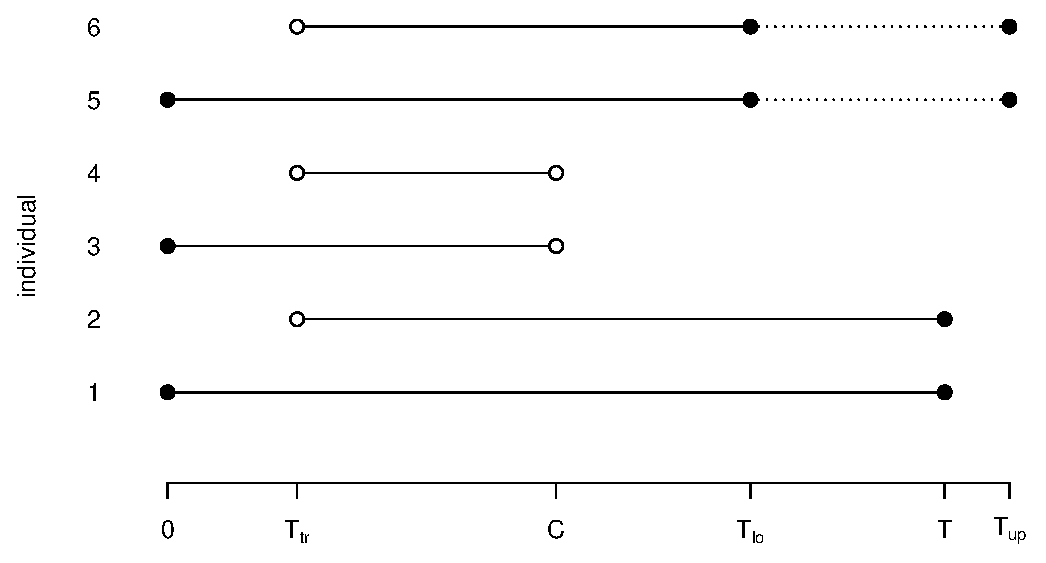
\epsfig{file=grafiken/censoringschemes.eps,scale=0.7}
{\it\caption{Illustration of different censoring
schemes.\label{censoringschemes}}}
\end{center}
\end{figure}

In a general framework an observation can now be uniquely described
 by the quadruple $(T_{tr},T_{lo},T_{up},\delta)$, with
\begin{center}
\begin{tabular}{ll}
$T_{lo}=T_{up}=T$, $\delta=1$ & if the observation is uncensored,\\
$T_{lo}=T_{up}=C$, $\delta=0$ & if the observation is right censored,\\
$T_{lo}<T_{up}$, $\delta=0$ & if the observation is interval censored.\\
\end{tabular}
\end{center}
For left truncated observations we have $T_{tr}>0$ while $T_{tr}=0$
for observations which are not truncated.

Based on these definitions we can now construct the likelihood
contributions for the different censoring schemes in terms of the
hazard rate $\lambda(t)$ and the survivor function
$S(t)=\exp(\int_0^t\lambda(u)du)$. Under the common assumption of
noninformative censoring and conditional independence, the
likelihood is given by
\begin{equation}\label{likelihood}
 L=\prod_{i=1}^n L_i,
\end{equation}
where
\[L_i = \lambda(T_{up})S(T_{up})/S(T_{tr}) = \lambda(T_{up})\exp\left(-\int_{T_{tr}}^{T_{up}}\lambda(t)dt\right)\]
for an uncensored observation,
\[L_i = S(T_{up})/S(T_{tr}) = \exp\left(-\int_{T_{tr}}^{T_{up}}\lambda(t)dt\right)\]
for a right censored observation and
\[L_i = (S(T_{lo})-S(T_{up}))/S(T_{tr}) = \exp\left(-\int_{T_{tr}}^{T_{lo}}\lambda(t)dt\right)\left(1-\exp\left(-\int_{T_{lo}}^{T_{up}}\lambda(t)dt\right)\right)\]
for an interval censored observation. Note that for explicit
evaluation of the likelihood (\ref{likelihood}) some numerical
integration technique has to be employed, since none of the
integrals can in general be solved analytically.

The above notation also allows for the easy inclusion of piecewise
constant, time-varying covariates via some data augmentation. Noting
that
\[\int_{T_{tr}}^{T}\lambda(t)dt = \int_{T_{tr}}^{t_1}\lambda(t)dt + \int_{t_1}^{t_2}\lambda(t)dt + \ldots + \int_{t_{p-1}}^{t_p}\lambda(t)dt + \int_{t_p}^{T}\lambda(t)dt\]
for $T_{tr}<t_1<\ldots<t_q<T$, we can replace an observation
$(T_{tr},T_{lo},T_{up},\delta)$ by a set of new observations
$(T_{tr},t_1,t_1,0)$, $(t_1,t_2,t_2,0)$, \ldots
$(t_{p-1},t_p,t_p,0)$, $(t_{p},T_{lo},T_{up},\delta)$ without
changing the likelihood. Therefore, observations with time-varying
covariates can be split up into several observations, where the
values $t_1<\ldots<t_p$ are defined by the changepoints of the
covariate and the covariate is now time-constant on each of the
intervals. In theory, other paths for a covariate $x(t)$ than
piecewise constant ones are also possible, if $x(t)$ is known for
$T_{tr}\le t\le T_{lo}$. In this case the the likelihood
(\ref{likelihood}) can also be evaluated numerically but a general
path $x(t)$ may lead to complicated data structures.

Figure \ref{timevaryingcovs} illustrates the data augmentation step
for a left truncated, uncensored observation and a covariate $x(t)$
that takes the three different values $x_1,x_2$ and $x_3$ on the
three intervals $[T_{tr},t_1], [t_1,t_2]$ and $[t_2,T_{up}]$. Here,
the original observation $(T_{tr},T_{up},T_{up},1)$ has to be
replaced by $(T_{tr},t_1,t_1,0)$, $(t_1,t_2,t_2,0)$ and
$(t_2,T_{up},T_{up},1)$.
\begin{figure}[htb]
\begin{center}
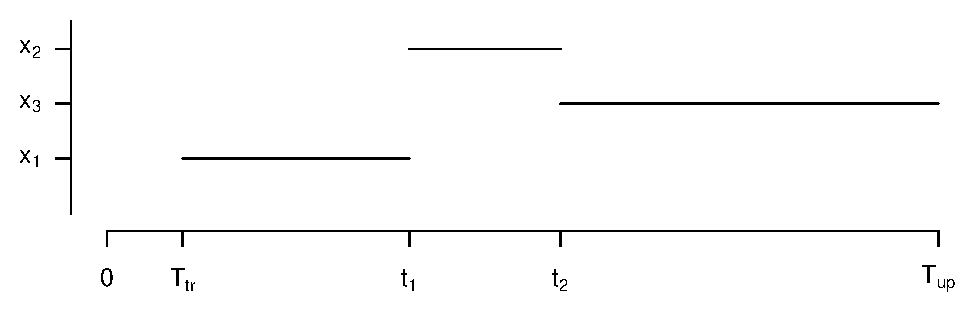
\epsfig{file=grafiken/timevaryingcovs.eps,scale=0.7}
{\it\caption{Illustration of time-varying
covariates.\label{timevaryingcovs}}}
\end{center}
\end{figure}

Currently, interval censored survival times can only be handled with
{\em remlreg objects}.

\subsection{Continuous-time multi-state models}\label{msmodels}
\index{Multi-state models}\index{Recurrent Events}\index{Disease
progression}\index{Competing risks}

Multi-state models are a flexible tool for the analysis of
time-continuous phenomena that can be characterized by a discrete
set of states. Such data structures naturally arise when observing a
discrete response variable for several individuals or objects over
time. Some common examples are depicted in Figure~\ref{some_msms} in
terms of their reachability graph for illustration. For recurrent
events (Figure~\ref{some_msms} (a)), the observations evolve through
time moving repeatedly between a fixed set of states. Other model
classes involve absorbing states, for example disease progression
models (Figure~\ref{some_msms} (b)), that are used to describe the
chronological development of a certain disease. If the severity of
this disease can be grouped into $q-1$ ordered stages of increasing
severity, a reasonable model might look like this: Starting from
disease state '$j$', an individual can only move to contiguous
states, i.e. either the disease gets worse and the individual moves
to state '$j+1$', or the disease attenuates and the individual moves
to state '$j-1$'. In addition, death is included as a further,
absorbing state '$q$', which can be reached from any of the disease
states. A model with several absorbing states is the competing risks
model (Figure~\ref{some_msms} (c)) where, for example, different
causes of death are analysed simultaneously.

\begin{figure}
\begin{center}
  \vspace{3mm}
 \mbox
 {
 \beginpicture
 \setcoordinatesystem units <0.65cm,0.65cm> point at 0 0
 \setlength{\unitlength}{0.65cm}

 \put {(a) Recurrent events} [Bl] at 0 16.5

 \put {\circle{1}} [Bl] at 7.5 12
 \put {\bf3} [Bl] at 7.35 11.85

 \put {\circle{1}} [Bl] at 5.5 14.5
 \put {\circle{1}} [Bl] at 9.5 14.5
 \put {\bf1} [Bl] at 5.35 14.35
 \put {\bf2} [Bl] at 9.35 14.35

 \arrow <3mm> [0.2,0.5] from 6.3 14.65 to 8.7 14.65
 \arrow <3mm> [0.2,0.5] from 8.7 14.35 to 6.3 14.35

 \arrow <3mm> [0.2,0.5] from  5.55 13.85 to 6.9 12.65
 \arrow <3mm> [0.2,0.5] from  7.25 12.65 to 5.9 13.85

 \arrow <3mm> [0.2,0.5] from  9.1 13.85 to 7.75 12.65
 \arrow <3mm> [0.2,0.5] from  8.1 12.65 to 9.45 13.85


 \put {(b) Disease progression} [Bl] at 0 10.5

 \put {\circle{1}} [Bl] at 7.5 6
 \put {$q$} [Bl] at 7.35 5.85

 \put {\circle{1}} [Bl] at 1.5 9
 \put {\circle{1}} [Bl] at 4.5 9
 \put {\circle{1}} [Bl] at 7.5 9
 \put {\circle{1}} [Bl] at 13.5 9
 \put {\bf1} [Bl] at 1.35 8.85
 \put {\bf2} [Bl] at 4.35 8.85
 \put {\bf3} [Bl] at 7.35 8.85
 \put {$q$-1} [Bl] at 13.15 8.85

 \put{$\cdots$} [Bl] at 10.1 8.9

 \arrow <3mm> [0.2,0.5] from 2.2 9.15 to 3.8 9.15
 \arrow <3mm> [0.2,0.5] from  3.8 8.85 to 2.2 8.85

 \arrow <3mm> [0.2,0.5] from 5.2 9.15 to 6.8 9.15
 \arrow <3mm> [0.2,0.5] from  6.8 8.85 to 5.2 8.85

 \arrow <3mm> [0.2,0.5] from 8.2 9.15 to 9.8 9.15
 \arrow <3mm> [0.2,0.5] from  9.8 8.85 to 8.2 8.85

 \arrow <3mm> [0.2,0.5] from 11.2 9.15 to 12.8 9.15
 \arrow <3mm> [0.2,0.5] from  12.8 8.85 to 11.2 8.85

 \arrow <3mm> [0.2,0.5] from  7.5 8.35 to 7.5 6.65
 \arrow <3mm> [0.2,0.5] from  4.75 8.35 to 7.0 6.65
 \arrow <3mm> [0.2,0.5] from  1.75 8.35 to 6.5 6.5
 \arrow <3mm> [0.2,0.5] from  13.25 8.35 to 8.5 6.5

 \put {(c) Competing risks} [Bl] at 0 4.5

 \put {\circle{1}} [Bl] at 1.5 0
 \put {\circle{1}} [Bl] at 4.5 0
 \put {\circle{1}} [Bl] at 7.5 0
 \put {\circle{1}} [Bl] at 13.5 0
 \put {\bf2} [Bl] at 1.35 -0.15
 \put {\bf3} [Bl] at 4.35 -0.15
 \put {\bf4} [Bl] at 7.35 -0.15
 \put {$q$} [Bl] at 13.35 -0.15

 \put {\circle{1}} [Bl] at 7.5 3
 \put {\bf1} [Bl] at 7.35 2.85

 \put{$\cdots$} [Bl] at 10.1 -0.1

 \arrow <3mm> [0.2,0.5] from  7.5 2.35 to 7.5 0.65

 \arrow <3mm> [0.2,0.5] from  6.9 2.6 to 4.75 0.65
 \arrow <3mm> [0.2,0.5] from  6.5 2.75 to 1.95 0.65
 \arrow <3mm> [0.2,0.5] from  8.5 2.75 to 12.85 0.65

 \endpicture
 }
 \vspace{3mm}

 \caption{Reachability graphs of some common multi-state
 models.\label{some_msms}}
\end{center}
\end{figure}

A multi-state model is fully described by a set of hazard rates
$\lambda_{hi}(t)$ where $h$, $h=1,\ldots,k$, indexes the type of the
transition and $i$, $i=1,\ldots,n$, indexes the individuals. Since
the hazard rates describe durations between transitions, we specify
them in analogy to hazard rate models for continuous time survival
analysis. To be more specific, $\lambda_{hi}(t)$ is modelled in a
multiplicative Cox-type way as
\[
 \lambda_{hi}(t) = \exp(\eta_{hi}(t)),
\]
where
\begin{equation}\label{addpred}
 \eta_{hi}(t) = g_{h0}(t) + \sum_{l=1}^Lg_{hl}(t)u_{il}(t) +
 \sum_{j=1}^Jf_{hj}(x_{ij}(t)) + v_i(t)'\gamma_h +  b_{hi}
\end{equation}
is an additive predictor consisting of the following components:
\begin{itemize}
 \item A time-varying, nonparametric baseline effect $g_{h0}(t)$ common for all
 observations.
 \item Covariates $u_{il}(t)$ with time-varying effects $g_{hl}(t)$.
 \item Nonparametric effects $f_{hj}(x_{ij}(t))$ of continuous covariates
 $x_{ij}(t)$.
 \item Parametric effects $\gamma_h$ of covariates $v_i(t)$.
 \item Frailty terms $b_{hi}$ to account for unobserved
 heterogeneity.
\end{itemize}

For each individual $i$, $i=1,\ldots,n,$ the likelihood contribution
in a multi-state model can be derived from a counting process
representation of the multi-state model. Let $N_{hi}(t)$,
$h=1,\ldots,k$ be a set of counting processes counting transitions
of type $h$ for individual $i$. Consequently, $h=1,\ldots,k$ indexes
the observable transitions in the model under consideration and the
jumps of the counting processes $N_{hi}(t)$ are defined by the
transition times of the corresponding multi-state process for
individual $i$.

From classical counting process theory (see e.g. \citeasnoun{Andetal93}, Ch.~VII.2), the intensity processes $\alpha_{hi}(t)$
of the counting processes $N_{hi}(t)$ are defined as the product of the hazard rate for type $h$ transitions $ \lambda_{hi}(t)$
and a predictable at-risk indicator process $Y_{hi}(t)$, i.e.
\[
 \alpha_{hi}(t) = Y_{hi}(t) \lambda_{hi}(t),
\]
where the hazard rates are constructed in terms of covariates as in
(\ref{addpred}). The at-risk indicator $Y_{hi}(t)$ takes the value
one if individual $i$ is at risk for a type $h$ transition at time
$t$ and zero otherwise. For example, in the multi-state model of
Figure~\ref{some_msms}a), an individual in state 2 is at risk for
both transitions to state 1 and state 3. Hence, the at-risk
indicators for both the transitions '2 to 1' and '2 to 3' will be
equal to one as long as the individual remains in state 2.

Under mild regularity conditions, the individual log-likelihood
contributions can now be obtained from counting process theory as
\begin{equation}\label{loglike1}
 l_i = \sum_{h=1}^k\left[ \int_0^{T_i}\log(\lambda_{hi}(t))dN_{hi}(t) -
 \int_0^{T_i}\lambda_{hi}(t)Y_{hi}(t)dt\right],
\end{equation}
where $T_i$ denotes the time until which individual $i$ has been
observed. The likelihood contributions can be interpreted similarly
as with hazard rate models for survival times (and in fact coincide
with these in the case of a multi-state process with only one
transition to an absorbing state). The first term corresponds to
contributions at the transition times since the integral with
respect to the counting process in fact equals a simple sum over the
transition times. Each of the summands is then given by the
log-intensity for the observed transition evaluated at this
particular time point. In survival models this term simply equals
the log-hazard evaluated at the survival time for uncensored
observations. The second term reflects cumulative intensities
integrated over accordant waiting periods between two successive
transitions. The integral is evaluated for all transitions the
corresponding person is at risk at during the current period. In
survival models there is only one such transition (the transition
from 'alive' to 'dead') and the integral is evaluated from the time
of entrance to the study to the survival or censoring time.

More details on multi-state models, including an exemplary analysis on human sleep, can be found in \citeasnoun{KneHen06}.

\section{Multilevel structured additive distributional and quantile regression}\label{distreg_star}

\subsection{Distributional regression}



Structured additive regression models assume that the distribution of the response variable $y$, given covariates $\xvec$ and $\uvec$, belongs to an exponential family. The conditional mean $\mu_i = E(y_i|\xvec,\uvec)$ is linked to a structured additive predictor
\begin{align*}
\eta_i = f_1(x_{i1}) + \ldots + f_p(x_{ip}) + \uvec_i' \gammavec, \,\,\,\,\,\,\,\, i = 1, \ldots, n,
\end{align*}
by $\mu_i = h(\eta_i)$, see Chapter \ref{obsmodel}. In matrix notation we obtain for the predictor
$$
\etavec = \Xvec_1 \betavec_1 + \ldots + \Xvec_p \betavec_p + \Uvec \gammavec,
$$
see again Chapter \ref{obsmodel} for details.
For the most basic model with Gaussian responses  and the  identity response function we have
\begin{align*}
y_i \sim  \mathcal{N}(\eta_i, \sigma^2) = \mathcal{N}(f_1(x_{i1}) + \ldots + f_p(x_{ip}) + \uvec_i' \gammavec,\sigma^2)
\end{align*}
or
$$
\yvec = \mathcal{N}(\etavec, \sigma^2 \Ivec) = \mathcal{N}(\Xvec_1 \betavec_1 + \ldots + \Xvec_p \betavec_p + \Uvec \gammavec,\sigma^2 \Ivec).
$$


Here and in other convential STAR models only the conditional mean is modeled in dependence of covariates.

A more flexible approach is given by distributional regression as introduced in  \citeasnoun{kleknelan14a} and \citeasnoun{kleknelan14b}. On the one hand, the class of distributions that can be estimated with distributional regression is no longer restricted to the exponential family. On the other hand, distributional regression allows to model not only the conditional mean of the response variable but the whole set of distribution parameters $\varthetavec_1,\ldots,\varthetavec_K$, i.e.~all $K$ parameters of the response distribution can be related to a set of predictor variables, which of course may vary between the different parameters. Using response functions $h_1, \ldots, h_K$ each of these parameters can be linked to a structured additive predictor via
\[
\varthetavec_k = h_k(\etavec_k) = h_k(\Xvec_{1k} \betavec_{1k} + \ldots + \Xvec_{pk} \betavec_{pk} + \Uvec_k \gammavec_k), \quad k=1,\ldots,K.
\]
Usually, the response functions are chosen to ensure appropriate restrictions on the parameter spaces. We use, for example, the exponential function to ensure positivity of the scale parameter.

Presumably the most simple distributional regression model is obtained with Gaussian responses where both the mean $\mu$ and the variance
$\sigma^2$ is modeled in terms of covariates.
Thus, we consider a regression model with
\begin{align*}
\begin{array}{lllll}
\muvec & = & h_1(\etavec_1) & = & \etavec_1, \\ [0.2cm]
\sigmavec^2 & = & h_2(\etavec_2) & = & \exp(\etavec_2).
\end{array}
\end{align*}

A possible generalization of the normal distribution is given by the three-parameter Student's t distribution with location parameter $\mu$, scale parameter $\sigma^2>0$ and degrees of freedom $\texttt{df}>0$. The probability density function is given by
\begin{align*}
f(y|\mu, \sigma, df) = \frac{\Gamma\left( \frac{df +1 }{2}\right)}{\sigma \Gamma\left( \frac{1}{2}\right) \Gamma\left(
\frac{df}{2}\right)\sqrt{df}} \cdot \left( 1+ \frac{(y-\mu)^2}{\sigma^2 df}\right)^{-\frac{df+1}{2}},
\end{align*}
where $\Gamma(x) = \int_0^{\infty} u^{x-1} \exp(-u) \mathrm{d}u$ for $x>0$ is the gamma function. Similar to the normal distribution the t distribution is symmetric and bell-shaped but it has heavier tails, offering a robust alternative to the normal distribution. For $\texttt{df} \rightarrow \infty$ it collapses to the normal distribution.

Regarding the positivity of $\sigma^2$ and $\texttt{df}$ we consider the model
\begin{align*}
\begin{array}{lllll}
\muvec & = & h_1(\etavec_1) & = & \etavec_1, \\ [0.2cm]
\sigmavec^2 & = & h_2(\etavec_2) & = & \exp(\etavec_2), \\ [0.2cm]
\boldsymbol{\texttt{df}} & = & h_3(\etavec_3) & = & \exp(\etavec_3). \\ [0.2cm]
\end{array}
\end{align*}

A popular two parameter distribution for modeling skewed distributions is the gamma distribution with mean parameter $\mu>0$ and shape parameter $\sigma>0$. The probability density function is given by
\begin{equation*}
f(y_i|\mu_i, \sigma_i) = \left( \frac{\sigma_i}{\mu_i} \right)^{\sigma_i} \cdot \frac{y_i^{\sigma_i-1}}{\Gamma(\sigma_i)} \cdot \exp\left(- \frac{\sigma_i}{\mu_i} \cdot y_i \right),
\end{equation*}
The mean of the gamma distribution corresponds to $\mu$, the variance is given by $\mu^2/\sigma$.
Setting up a regression model both the mean and the shape parameter are linked to a STAR predictor via the exponential function due to the positivity constraints:
\begin{align*}
\begin{array}{lllll}
\muvec & = & h_1(\etavec_1) & = & \exp(\etavec_1), \\ [0.2cm]
\sigmavec & = & h_2(\etavec_2) & = & \exp(\etavec_2).
\end{array}
\end{align*}

A comprehensive list of all distributional regression models available in BayesX can be found in Tables \ref{tab:distrBayesX1}  to \ref{tab:distrBayesX4} of the Reference Manual.


\subsection{Quantile Regression} \label{sec:quantreg}

 Distributional regression assumes a specific parametric probability distribution of the response (like the normal, lognormal or gamma distribution) and models some or all of its parameters in dependence of covariates. Quantile regression, in contrast, is a distribution-free approach, trying to directly model the different quantiles of the response as a function of covariates.

In linear quantile regression (see  \citeasnoun{Koe05}), we assume
\begin{align*}
q_{\varphi,i} = \beta_{\varphi,0} + \beta_{\varphi,1}x_{i1} + \ldots + \beta_{\varphi,p}x_{ip}
\end{align*}
where $q_\varphi$, for $\varphi \in (0,1)$, is the $\varphi$-quantile of the response distribution. Estimation of the quantile-specific regression coefficients $\betavec_{\varphi}$ relies on minimizing the asymmetrically weighted error (AWE) criterion
\begin{align}
\hat{\betavec}_{\varphi} = \mbox{argmin}_{\betavec_{\varphi}} \left\{ \sum_{i=1}^{n} \rho_{\varphi}(y_i - \xvec_i' \betavec_{\varphi})\right\},
\label{eq:quantmin}
\end{align}
with the loss function $\rho_{\varphi}$ defined by
\begin{align*}
\rho_{\varphi}(u) = \begin{cases} u \varphi & \textnormal{if $u \geq 0$} \\ u (\varphi - 1) & \textnormal{if $u < 0$,} \end{cases}
\end{align*}
which is also known as the check function. Since there exists no closed form solution for this minimization problem, estimates are typically obtained based on linear programming and modifications of the simplex algorithm, see \citeasnoun{Koe05} for details. The distribution of the response is implicitly determined by the estimated quantiles $q_{\varphi}$ provided that quantiles for a reasonable dense grid of $\varphi$-values are estimated. Generalizations to structured additive predictors are conceptually straightforward. However, estimation is highly challenging and almost impossible for complex hierarchical models, revealing the limits of frequentist quantile regression.

Bayesian structured quantile regression requires a distributional assumption for the responses to be able to set up a likelihood. Following \citeasnoun{WalKneLanYue12} we will assume independent and identically distributed observations following an asymmetric Laplace distribution with location parameter $\eta_{i,\varphi}$ (specified in the usual structured additive fashion), scale parameter $\sigma^2$ and skewness parameter $\varphi$,
\begin{align*}
y_{i} | \eta_{i,\varphi}, \sigma^2, \varphi \overset{\textnormal{iid}}{\sim} \textnormal{ALD}(\eta_{i,\varphi},\sigma^2,\varphi).
\end{align*}
Then, the density of the responses is given by
\begin{align*}
p(y_i | \eta_{i,\varphi},\sigma^2,\varphi) = \frac{\varphi(1-\varphi)}{\sigma^2} \exp\left(-\frac{\rho_{\varphi}(y_i - \eta_i{\varphi})}{\sigma^2}\right).
\end{align*}
Maximizing the corresponding posterior (for fixed $\sigma^2$ and $\varphi$) obviously is equivalent to minimizing the AWE criterion (\ref{eq:quantmin}) in case of a linear predictor. However, in contrast to frequentist quantile regression the linear predictor can be replaced by a hierarchical structured additive predictor without any further difficulties, see \citeasnoun{WalKneLanYue12} for details.

Since the check function $\rho_{\varphi}$ is non-differentiable, inference based on Markov chain Monte Carlo (MCMC) simulations at a first glance seems to be complicated. However, the asymmetric Laplace distribution can be represented as a scaled mixture of normals
\begin{align*}
Y_i = \eta_i + \xi W_i + \delta Z_i \sqrt{\sigma^2 W_i}
\end{align*}
with $\xi = \frac{1-2\varphi}{\varphi(1-\varphi)}$ and $\delta^2 = \frac{2}{\varphi(1-\varphi)}$.  $W_i \sim \textnormal{Exp}(\frac{1}{\sigma^2})$ and $Z_i \sim \mathcal{N}(0,1)$ are independent random variables following an exponential distribution with mean $\sigma^2$ and a standard normal distribution, respectively. Thus, using offsets $\xi W_i$ and weights $\delta \sqrt{\sigma^2 W_i}$ the Bayesian quantile regression problem can be interpreted as a conditionally Gaussian regression model after imputing $W_i$ as a part of the MCMC sampler.


\subsection{Multilevel models}
\label{star_multilevel}

Recently \citeasnoun{LanUml14} have proposed  a multilevel version of STAR models to cope with the hierarchical nature of many data sets.
Suppose that covariate $x_j \in \{1,\dots,K\}$ is a unit- or cluster index   and $x_{ij}$ indicates the cluster
observation $i$ pertains to.
Then the design  matrix $\mathbf{X}_j$ is a $n \times K$ incidence matrix with $\mathbf{X}_j[i,k] = 1$ if the $i$-th observation
belongs to cluster $k$ and zero else. The $K \times 1$ parameter vector $\boldsymbol{\beta}_j$ is the vector of regression parameters,
i.e.~the $k$-th element
in $\boldsymbol{\beta}_j$ corresponds to the regression coefficient of the $k$-th cluster.
We now define a second level equation
\begin{equation}
\label{eq:compprior}
\boldsymbol{\beta}_j = \boldsymbol{\eta}_j + \boldsymbol{\varepsilon}_j =
\mathbf{X}_{j1} \boldsymbol{\beta}_{j1} + \ldots + \mathbf{X}_{jp_j} \boldsymbol{\beta}_{jp_j} +
\mathbf{U}_j \boldsymbol{\gamma}_j +  \boldsymbol{\varepsilon}_j,
\end{equation}
where the terms $\mathbf{X}_{j1} \boldsymbol{\beta}_{j1},\dots,\mathbf{X}_{jp_j} \boldsymbol{\beta}_{jp_j}$ correspond to additional nonlinear
functions $f_{j1},\dots,f_{jp_j}$ and
$\mathbf{U}_j \boldsymbol{\gamma}_j$ comprises additional linear effects of cluster level covariates.
The ``errors'' $\boldsymbol{\varepsilon}_j \sim N(\mathbf{0}, \tau^2_j \mathbf{I})$
comprise a vector of i.i.d.\ Gaussian random effects.
Using the compound prior (\ref{eq:compprior}) we obtain an additive
decomposition of the cluster specific effect. By allowing a full STAR predictor (as in the level-1 equation), a rather complex decomposition of
the cluster effect
$\boldsymbol{\beta}_j$ including interactions is possible. A special case arises if cluster specific covariates are not available. Then the
prior for $\boldsymbol{\beta}_j$ collapses to
$\boldsymbol{\beta}_j = \boldsymbol{\varepsilon}_j \sim N(\mathbf{0}, \tau^2_j \mathbf{I})$ and we obtain a simple i.i.d. Gaussian cluster
specific random effect with variance parameter $\tau^2_j$.

A third or fourth level in the hierarchy is possible by assuming that the second or third level regressions
contain additional cluster-specific random effects whose parameters are again modeled through  STAR predictors of cluster level covariates.



%In a multilevel STAR model (\shortciteN{lanuml14}) the regression coefficients $\betavec_j$ of a function $f_j$ may themselves obey a regression model with a structured additive predictor, i.e.
%\begin{align}
%\betavec_j \sim  \mathcal{N}(\boldsymbol{\eta}_j,\tau^2_j \mathbf{I}) =
%\mathcal{N}(\Zvec_{j1} \betavec_{j1} + \ldots + \Zvec_{jq_j} \betavec_{jq_j} + \Xvec_j \gammavec_j, \tau^2_j \mathbf{I})
%\label{eq:compprior}
%\end{align}
%where the terms $\mathbf{Z}_{j1} \boldsymbol{\beta}_{j1},\dots,\mathbf{Z}_{jq_j} \boldsymbol{\beta}_{jq_j}$ represent additional nonlinear functions $f_{j1},\dots,f_{jq_j}$, and  $\mathbf{X}_j \boldsymbol{\gamma}_j$ comprises additional linear effects.
%Further levels are possible by assuming that the second level regression parameters $\boldsymbol{\beta}_{jl}$, \linebreak $l=1,\dots,q_j$, again obey a STAR model.
%
%In this paper we use the compound prior (\ref{eq:compprior}) if a covariate $z_j \in \{1,\dots,K\}$ is a spatial index and $z_{ij}$ indicates the region observation $i$ pertains to. Then, the design matrix $\mathbf{Z}_j$ is a $n \times K$ incidence matrix with $\mathbf{Z}_j[i,k] = 1$ if the $i$-th observation belongs to region $k$ and zero else. The $K \times 1$ parameter vector $\boldsymbol{\beta}_j$ is the vector of regression parameters, i.e.~the $k$-th element in $\boldsymbol{\beta}$ corresponds to the regression coefficient of the $k$-th region. The use of the compound prior (\ref{eq:compprior}) allows for further explaining the region specific effect by spatial covariates.
%
%The hierarchical structure of the Austrian political-administrative units suggests a four level regression model: Single-family homes (level-1) belong to municipalities (level-2), which are nested in districts (level-3), which are themselves nested in counties (level-4). Assuming house prices per square meter to be normally distributed leads to the following four level STAR model, see also  \shortciteN{brulan11}:
%\begin{align}
%\begin{array}{llll}
%\mbox{level-1:} & \mathit{\boldsymbol{p_{qm}}} &  = & \fvec_1(\mathit{area}) + \fvec_2(\mathit{area\_plot}) + \fvec_3(\mathit{age}) + \fvec_4(\mathit{time\_index}) + \\
%                &              &    & \fvec_5(\mathit{muni}) + \Xvec \gammavec + \varepsilonvec \\
%                &              &  = & \Zvec_1 \betavec_1 + \Zvec_2 \betavec_2 + \Zvec_3 \betavec_3 + \Zvec_4 \betavec_4 + \Zvec_5 \betavec_5 + \Xvec \gammavec + \varepsilonvec  \\ [0.2cm]
%\mbox{level-2:} & \betavec_5   &  = & \fvec_{5,1}(\mathit{pp\_ind}) + \fvec_{5,2}(\mathit{ln\_educ}) +  \fvec_{5,3}(\mathit{age\_ind}) + \fvec_{5,4}(\mathit{comm}) + \\
%                &              &    & \fvec_{5,5}(\mathit{ln\_den}) + \fvec_{5,6}(\mathit{dist}) + \varepsilonvec_5      \\
%                &              &  = & \Zvec_{5,1} \betavec_{5,1} + \Zvec_{5,2} \betavec_{5,2} + \Zvec_{5,3} \betavec_{5,3} + \Zvec_{5,4} \betavec_{5,4} +  \\
%                &              &    & \Zvec_{5,5} \betavec_{5,5} + \Zvec_{5,6} \betavec_{5,6} + \varepsilonvec_5  \\ [0.2cm]
%\mbox{level-3:} & \betavec_{5,6} & = & \fvec_{5,6,1}(\mathit{wko\_ind}) + \fvec_{5,6,2}^{mrf}(\mathit{dist}) + \fvec_{5,6,3}(\mathit{county}) + \varepsilonvec_{5,6} \\
%                &                & = & \Zvec_{5,6,1} \betavec_{5,6,1} + \Zvec_{5,6,2} \betavec_{5,6,2} + \Zvec_{5,6,3} \betavec_{5,6,3} + \varepsilonvec_{5,6} \\ [0.2cm]
%\mbox{level-4:} & \betavec_{5,6,3} & = & \mathds{1} \gamma_0 + \varepsilonvec_{5,6,3}. \\
%\end{array}
%\label{eq:model}
%\end{align}
%
%The categorical covariates on level-1, describing the quality and equipment of the house, are encoded as dummy variables and subsumed in the design matrix $\Xvec$ with estimated parameters $\gammavec$. The possibly nonlinear functions $\fvec_1,\fvec_2,\dots$ are modeled by P-splines.
%
%The level-1 equation contains an uncorrelated random municipality effect $f_5(\emph{muni})$, controlling for unordered spatial heterogeneity. This municipality-specific heterogeneity is modeled through the level-2 equation and is further decomposed into a district and finally into a county level effect (levels 3 and 4). Furthermore, district specific spatial heterogeneity is modeled through a correlated spatial effect $f_{5,6}(\emph{dist})$ in the level-3 equation by Markov random fields, denoted by the superscript "\emph{mrf}", see \shortciteN{fahkne13} for details regarding MRF's.
%
%From model (\ref{eq:model}) we immediately get the conditional mean of the house price per square meter $p_{qm}$. The $\varphi$-th conditional quantile of the house price per square meter is given by
%\begin{equation}
%Q_{\varphi}(p_{qm}) = \EV(p_{qm}) + \sigma \cdot \Phi^{-1}(\varphi),
%\label{eq:quantnormal}
%\end{equation}
%with $\Phi^{-1}(\varphi)$ being the $\varphi$-th quantile of the standard normal distribution. The variance parameter $\sigma^2$ (and so the standard deviation $\sigma$) can be replaced by a suitable estimator.
%%by the sample variance
%%\begin{align*}
%%\widehat{\sigma^2} = S^2 = \frac{\sum_{i=1}^n (p_{qm_i}-\widehat{p_{qm_i}})^2}{n-k},
%%\end{align*}
%%where $k$ denotes the total degrees of freedom.
%Equation (\ref{eq:quantnormal}) shows that the quantiles can be received by simply shifting the mean according to the estimated variance.
%
%Due to the additive structure of our model the conditional quantiles of the house price per square meter change additively with changes in values of covariates. Subsequently, the conditional quantiles of the total house price $p$ change proportionally to the floor area of the building:
%\begin{align*}
%\begin{array}{lll}
%Q_{\varphi}(p) & = & area \cdot \left(\eta + \sigma \cdot \Phi^{-1}(\varphi)\right)\\ [0.2cm]
%     & = & area \cdot \left(f_1(area)+ \ldots + f_5(muni)+\gamma_1 x_1 + \ldots  +\gamma_p x_p + \sigma \cdot \Phi^{-1}(\varphi)\right).
%\end{array}
%\end{align*}
%
%Therefore, if for example covariate $x_1$ changes by one unit, the predictor $\eta$ -- and so the considered quantile of the price per square meter -- changes additively by $\gamma_1$. The quantile of the total price then changes by $area \cdot \gamma_1$. Thus, the change in the quantiles of the price is proportional to the floor area of the building. Turning to the nonlinear effects, let $f(z)$ be the nonlinear effect of a covariate $z$, and let $\mathrm{d}f(z) = f(z+1) - f(z)$. Then, analogously, the quantile of the price per square meter changes by $\mathrm{d}f(z)$ and the quantile of the total price changes by $area \cdot \mathrm{d}f(z)$, again being proportional to the size of the house. Furthermore, since $f(.)$ is a nonlinear function, the change differs over the range of $z$. For the conditional mean we get analog results.
%%\subsubsection*{Lognormally distributed prices}
%%
%%In Section \ref{sec:data} we have seen that the empirical house prices per square meter seem to be approximately lognormally distributed instead of being Gaussian. Assuming the response \emph{$p_{qm}$} to be lognormally distributed, i.e.
%%\begin{align*}
%%\mathit{p_{qm}} \sim \mathcal{LN}(\mu, \sigma^2),
%%\end{align*}
%%leads to normally distributed logged house prices per square meter. Thus, one could guess to improve model (\ref{eq:model}) by replacing the response \emph{$p_{qm}$} by the logged house price per square meter \emph{$lnp_{qm}$}, i.e.
%%\begin{align}
%%\mathit{\boldsymbol{lnp_{qm}}} = \boldsymbol{\eta} + \varepsilonvec,
%%\label{eq:model2}
%%\end{align}
%%which we will call the \emph{Loggaussian model}, with the same hierarchical predictor $\boldsymbol{\eta}$ as before and the errors again being mutually independent normally distributed with mean $0$ and variance $\sigma^2$.
%
%For the loggausian model (\ref{loggaussianm})
%We receive the conditional quantiles of the house price per square meter by
%$$
%\begin{array}{lll}
%Q_{\varphi}(p_{qm}) & = & \exp\left(\eta + \sigma \cdot \Phi^{-1}(\varphi)\right) \\ [0.2cm]
%     & = & \exp\left(f_1(area)+ \ldots + f_5(muni)+\gamma_1 x_1 + \ldots  + \gamma_p x_p + \sigma \cdot \Phi^{-1}(\varphi)\right) \\ [0.2cm]
%     & = & \exp\left(f_1(area)\right) \ldots \exp\left(f_5(muni)\right) \exp(\gamma_1 x_1)  \ldots  \exp(\gamma_p x_p) \exp(\sigma \cdot \Phi^{-1}(\varphi)).
%\end{array}
%$$
%
%Obviously, the conditional quantiles of the house price per square meter $p_{qm}$ now change multiplicatively with changes in values of covariates. If for example covariate $x_1$ changes by one unit, the predictor $\eta$ again changes by $\gamma_1$, but the quantiles of the price per square meter now change multiplicatively by the factor $\exp(\gamma_1)$, yielding
%$$
%\begin{array}{lll}
%\Delta Q_{\varphi}(p_{qm}) & = & \exp(\eta + \sigma \cdot \Phi^{-1}(\varphi)) \cdot \exp(\gamma_1) - \exp(\eta + \sigma \cdot \Phi^{-1}(\varphi))\\ [0.2cm]
%     & = & \exp(\eta + \sigma \cdot \Phi^{-1}(\varphi)) \cdot \left(\exp(\gamma_1)-1\right).
%\end{array}
%$$
%For the conditional quantiles of the total prices we get:
%$$
%\begin{array}{lll}
%Q_{\varphi}(p) & = & area \cdot \exp(\eta + \sigma \cdot \Phi^{-1}(\varphi)) \\ [0.2cm]
%     & = & area \cdot \exp\left(f_1(area)\right) \ldots \exp\left(f_5(muni)\right) \exp(\gamma_1 x_1)  \ldots  \exp(\gamma_p x_p) \exp(\sigma \cdot \Phi^{-1}(\varphi)).
%\end{array}
%$$
%
%So, the quantiles of the total price change multiplicatively with changes in values of covariates too. If for example covariate $x_1$ changes by one unit, the quantiles of the total price change by
%\begin{align*}
%\Delta Q_{\varphi}(p) = area \cdot \exp(\eta + \sigma \cdot \Phi^{-1}(\varphi)) \cdot \left(\exp(\gamma_1)-1\right),
%\end{align*}
%making the change again proportional to the floor area. Similarly, if covariate $z$ (representing a nonlinear effect) changes by one unit, both the conditional quantiles of prices per square meter and the conditional quantiles of total prices multiplicatively change by the factor $\exp\left(\mathrm{d}f(z)\right)$, since
%$$
%\exp\left(f(z+1)\right) = \exp\left(f(z+1)-f(z)+f(z)\right) = \exp\left(\mathrm{d}f(z)\right)\exp\left(f(z)\right).
%$$
%Therefore, the change in the quantiles of total prices caused by a change in any covariate again is proportional to the floor area of the building.
%
%
%For the conditional mean of the house price per square meter
%\begin{align*}
%\EV(p_{qm}) = \exp(\eta + \sigma^2/2)
%\end{align*}
%we get analog results.
%




\addcontentsline{toc}{section}{Bibliography}

\begin{thebibliography}{99}


\harvarditem{Albert \& Chib}{1993}{AlbChi93}
 {\scshape Albert, J. \& Chib, S.} (1993).
 Bayesian Analysis of Binary and Polychotomous Response Data.
 {\it Journal of the American Statistical Association}, {\bf 88}, 669--679.

\harvarditem{Andersen et al.}{1993}{Andetal93}
 {\scshape Andersen, P. K., Borgan, {\O}, Gill, R. D. \& Keiding, N.} (1993).
 {\it Statistical Models Based on Counting Processes.}
 New York: Springer Verlag.

\harvarditem{Andrews \& Mallows}{1974}{AndMal74}
 {\scshape Andrews, D. F. \& Mallows, C. L.} (1974).
 Scale mixtures of Normal Distributions.
 {\it Journal of the Royal Statistical Society B}, {\bf 36}, 99--102.

\harvarditem{Bollaerts, Eilers \& van Mechelen}{2006}{BolEilvMe06}
 {\scshape Albert, J. \& Chib, S.} (1993).
 Simple and Multiple P-Spline Regression with Shape Constraints.
 {\it British Journal of Mathematical and Statistical Psychology}, {\bf 59}, 451--469.

\harvarditem{Belitz}{2007}{Bel07}
 {\scshape Belitz, C.} (2007).
 {\it Model Selection in Generalized Structured Additive Regression Models.}
 PhD Thesis, University of Munich.

\harvarditem{Belitz \& Lang}{2008}{BelLan08}
{\scshape Belitz, C. \& Lang, S.} (2008).
 Simultaneous Selection of Variables and Smoothing Parameters in Structured Additive Regression Models.
{\it Computational Statistics and Data Analysis}, {\bf 53} , 61-81.

\harvarditem{Besag, York \& Molli\'{e}}{1991}{BesYorMol91}
 {\scshape Besag, J., York, J. \& Molli\'{e}, A.} (1991).
 Bayesian Image Restoration with two Applications in Spatial Statistics (with discussion).
 {\it Annals of the Institute of Statistical Mathematics}, {\bf 43}, 1--59.

\harvarditem{Brezger \& Lang}{2006}{BreLan06}
 {\scshape Brezger, A. \& Lang, S.} (2006).
 Generalized Additive Regression based on Bayesian P-Splines.
 {\it Computational Statistics and Data Analysis} {\bf 50}, 967--991.

\harvarditem{Devroye}{1986}{Dev86}
 {\scshape Devroye, L.} (1986).
 {\it Non-Uniform Random Variate Generation.}
 New York: Springer Verlag.

\harvarditem{Eilers \& Marx}{1996}{EilMar96}
 {\scshape Eilers, P. H. C. \& Marx, B. D.} (1996).
 Flexible Smoothing using B-Splines and Penalized Likelihood (with comments and rejoinder).
 {\it Statistical Science}, {\bf 11}, 89--121.

\harvarditem{Fahrmeir, Kneib \& Lang}{2004}{FahKneLan04}
 {\scshape Fahrmeir, L., Kneib, T. \& Lang, S.} (2004).
 Penalized Structured Additive regression for Space-Time Data: A Bayesian Perspective.
 {\it Statistica Sinica}, {\bf 14}, 715--745.

\harvarditem{Fahrmeir et al.}(2013){fahkne13}
{\scshape Fahrmeir, L.,  Kneib, T., Lang, S. \& Marx, B.}{2013}
{\it Regression: Models, Methods and Applications.}
 New York: Springer-Verlag.


\harvarditem{Fahrmeir \& Lang}{2001}{FahLan01a}
 {\scshape Fahrmeir, L. \& Lang, S.} (2001a).
 Bayesian Inference for Generalized Additive Mixed Models Based on Markov Random Field Priors.
 {\it Journal of the Royal Statistical Society C}, {\bf 50}, 201--220.

\harvarditem{Fahrmeir \& Lang}{2001}{FahLan01b}
 {\scshape Fahrmeir, L. \& Lang, S.} (2001b).
 Bayesian Semiparametric Regression Analysis of Multicategorical Time-Space Data.
 {\it Annals of the Institute of Statistical Mathematics}, {\bf 53}, 10--30.

\harvarditem{Fahrmeir \& Osuna}{2006}{FahOsu06}
 {\scshape Fahrmeir, L. \& Osuna, L.} (2006).
 Structured Additive Regression for Overdispersed and Zero-Inflated Count Data.
 {\it Applied Stochastic Models in Business and Industry}, {\bf 22}, 351--369

 \harvarditem{Fahrmeir \& Tutz}{2001}{FahTut01}
 {\scshape Fahrmeir, L. \& Tutz, G.} (2001).
 {\it Multivariate Statistical Modelling based on Generalized Linear Models.}
 New York: Springer-Verlag.

\harvarditem{Fotheringham, Brunsdon \& Charlton}{2002}{FotBruCha02}
 {\scshape Fotheringham, A. S., Brunsdon, C., \& Charlton, M. E.} (2002).
 {\it Geographically Weighted Regression: The Analysis of Spatially Varying Relationships.}
 Chichester: Wiley.

\harvarditem{Gamerman}{1997}{Gam97}
 {\scshape Gamerman, D.} (1997).
 Efficient Sampling from the Posterior Distribution in Generalized Linear Models.
 {\it Statistics and Computing}, {\bf 7}, 57--68.

\harvarditem{Gelfand, Sahu \& Carlin}{1996}{GelSahCar96}
 {\scshape Gelfand, A. E., Sahu, S. K. \& Carlin, B. P.} (1996).
 Efficient Parametrizations for Genera\-lized Linear Mixed Models.
 In: Bernardo, J. M., Berger, J. O., Dawid, A. P. \& Smith, A. F. M. (eds.),
 {\it Bayesian Statistics 5}, 165--180.
 Oxford University Press.

\harvarditem{George \& Liu}{1981}{GeoLiu81}
 {\scshape George, A. \& Liu, J.W.} (1981).
 {\it Computer Solution of Large Sparse Positive Definite Systems.}
 Series in computational mathematics, Prentice-Hall.

\harvarditem{Green}{1987}{Gre87}
 {\scshape Green, P. J.} (1987).
 Penalized Likelihood for General Semiparametric Regression Models.
 {\it International Statistical Review}, {\bf 55}, 245--259.

\harvarditem{Green}{2001}{Gre01}
 {\scshape Green, P. J.} (2001).
 A Primer in Markov Chain Monte Carlo.
 In: Barndorff-Nielsen, O. E., Cox, D. R. \& Kl\"{u}ppelberg, C. (eds.),
 {\it Complex Stochastic Systems}, 1--62.
 Chapmann and Hall, London.

\harvarditem{Green \& Silverman}{1994}{GreSil94}
 {\scshape Green, P. J. \& Silverman, B.} (1994).
 {\it Nonparametric Regression and Generalized Linear Models.}
 Chapman and Hall, London.

\harvarditem{Griffin \& Brown}{2005}{GriBro05}
 {\scshape Griffin, J. E., and Brown, P. J.} (2005). Alternative Prior Distributions
 for Variable Selection with very many more Variables than Observations. Technical
 report, University of Warwick, Dept. of Statistics.

\harvarditem{Harville}{1977}{Har77}
 {\scshape Harville, D. A.} (1977).
 Maximum Likelihood Approaches to Variance Component Estimation and to related Problems.
 {\it Journal of the American Statistical Association}, {\bf 72}, 320--338.

\harvarditem{Hastie \& Tibshirani}{1990}{HasTib90}
 {\scshape Hastie, T. \& Tibshirani, R.} (1990).
 {\it Generalized Additive Models.}
 Chapman and Hall, London.

\harvarditem{Hastie \& Tibshirani}{1993}{HasTib93}
 {\scshape Hastie, T. \& Tibshirani, R.} (1993).
 Varying-Coefficient Models.
 {\it Journal of the Royal Statistical Society B}, {\bf 55}, 757--796.

\harvarditem{Hastie \& Tibshirani}{2000}{HasTib00}
 {\scshape Hastie, T. \& Tibshirani, R.} (2000).
 Bayesian Backfitting.
 {\it Statistical Science}, {\bf 15}, 193--223.

\harvarditem{Hastie, Tibshirani \& Firedman}{2001}{HasTibFri01}
 {\scshape Hastie, T., Tisbshirani, R. \& Friedman, J.} (2001).
 {\it The Elements of Statistical Learning: Data Mining, Inference and Prediction.}
 New York: Springer-Verlag.

\harvarditem{Hennerfeind, Brezger \& Fahrmeir}{2006}{HenBreFah06}
 {\scshape Hennerfeind, A., Brezger, A. \& Fahrmeir, L.} (2006).
 Geoadditive Survival Models.
 {\it Journal of the American Statistical Association}, {\bf 101}, 1065--1075.

\harvarditem{Holmes \& Held}{2006}{HolHel06}
 {\scshape Holmes, C., Held, L.} (2006).
 Bayesian Auxiliary Variable Models for Binary and Multinomial Regression.
 {\it Bayesian Analysis}, {\bf 1}, 145--168.

\harvarditem{Hurvich, Simonoff \& Tsai}{1998}{HurSimTsa98}
 {\scshape Hurvich, C. M., Simonoff, J. S. \& Tsai, C. L.} (1998).
 Smoothing Parameter Selection in Nonparametric Regression using an improved {A}kaike Information Criterion.
 {\it Journal of the Royal Statistical Society B}, {\bf 60}, 271--293.

\harvarditem{Ishwaran \& Rao}{2005}{IshRao05}
 {\scshape Ishwaran, H., and Rao, S. J.} (2005). Spike and Slab Variable
 Selection: Frequentist and Bayesian Strategies. {\it The Annals of Statistics},
 {\bf 33}, 730-773.

\harvarditem{Johnson, Moore \& Ylvisaker}{1990}{JohMooYlv90}
 {\scshape Johnson, M.E., Moore, L.M. \& Ylvisaker, D.} (1990).
 Minimax and Maximin Designs.
 {\it Journal of Statistical Planning and Inference}, {\bf 26}, 131--148.

\harvarditem{Kammann \& Wand}{2003}{KamWan03}
 {\scshape Kammann, E. E. \& Wand, M. P.} (2003).
 Geoadditive Models.
 {\it Journal of the Royal Statistical Society C}, {\bf 52}, 1--18.


\harvarditem{Klein et al.}{2014a}{KleDenKneLan14}
{\scshape Klein, N., Denuit, M., Kneib, T. \& Lang, S.}(2014).
Nonlife Ratemaking and Risk Management with Bayesian additive Models for Location, Scale and Shape.
{\it Insurance: Mathematics and Economics}, {\bf 55}, 225--249.


\harvarditem{Klein et al.}{2014b}{kleknelan14a}
{\scshape Klein, N., Kneib, T., Lang, S.}(2013).
Bayesian Structured Additive Distributional Regression.
{\it Under revision for Annals of Applied Statistics}.


\harvarditem{Klein, Kneib \& Lang}{2014}{kleknelan14b}
{\scshape Klein, N., Kneib, T. \& Lang, S.}(2014).
Bayesian Generalized Additive Models for Location, Scale and Shape for Zero-Inflated and Overdispersed Count Data.
To appear in {\it Journal of the American Statistical Association}, doi:10.1080/01621459.2014.912955.


\harvarditem{Klein et al.}{2014c}{KleKneLan14c}
{\scshape Klein, N., Kneib, T., Klasen, S. \& Lang, S.}(2014).
Bayesian Structured Additive Distributional Regression for Multivariate Responses.
To appear in {\it Journal of the Royal Statistical Society C}, doi:10.1111/rssc.12090.


\harvarditem{Koenker}{2005}{Koe05}
{\scshape Koenker, R.}(2005).
{\it Quantile Regression.}
Cambridge University Press, New York.



\harvarditem{Kneib}{2006}{Kne06}
 {\scshape Kneib, T.} (2006).
 Geoadditive Hazard Regression for Interval Censored Survival Times.
 {\it Computational Statistics and Data Analysis}, {\bf 51}, 777--792

\harvarditem{Kneib \& Hennerfeind}{2006}{KneHen06}
 {\scshape Kneib, T. \& Hennerfeind, A.} (2006).
 Bayesian Semiparametric Multi-State Models.
 {\it Statistical Modelling}, {\bf 8}, 169--198.

\harvarditem{Kneib \& Fahrmeir}{2006}{KneFah06}
 {\scshape Kneib, T. \& Fahrmeir, L.} (2006).
 Structured Additive Regression for Categorical Space-Time Data: A Mixed Model approach.
 {\it Biometrics}, {\bf 62}, 109--118.

\harvarditem{Kneib \& Fahrmeir}{2007}{KneFah07}
 {\scshape Kneib, T. \& Fahrmeir, L.} (2007).
 A Mixed Model Approach to Structured Hazard Regression.
 {\it Scandinavian Journal of Statistics}, {\bf 34}, 207--228.

\harvarditem{Kneib et al.}{2009}{Kne09}
 {\scshape Kneib, T., Konrath, S. und Fahrmeir, L.} (2009). High-dimensional
 Structured Additive Regression Models: Bayesian Regularisation, Smoothing and Predictive
 Performance. Department of Statistics, Technical Report No. 46, LMU Munich.

\harvarditem{Knorr-Held}{1999}{KnoHel99}
 {\scshape Knorr-Held, L.} (1999).
 Conditional Prior Proposals in Dynamic Models.
 {\it Scandinavian Journal of Statistics}, {\bf 26}, 129--144.

\harvarditem{Konrath et al.}{2008}{Kon08}
 {\scshape Konrath, S., Kneib, T., Fahrmeir, L.} (2008). Bayesian Regularisation
 in Structured Additive Regression Models for Survival Data. Department of Statistics,
 Technical Report No.35, LMU Munich.

\harvarditem{Lang \& Brezger}{2004}{LanBre04}
 {\scshape Lang, S. \& Brezger, A.} (2004).
 Bayesian P-Splines.
 {\it Journal of Computational and Graphical Statistics}, {\bf 13}, 183--212.

\harvarditem{Lang et al.}{2014}{LanUml14}
 {\scshape Lang, S., Umlauf, N., Wechselberger, P., Harttgen, K.  \& Kneib, T.} (2014).
 Multilevel Structured Additive Regression.
 {\it Statistics and Computing}, {\bf 24}, 223--238.


\harvarditem{Lin \& Zhang}{1999}{LinZha99}
 {\scshape Lin, X. \& Zhang, D.} (1999).
 Inference in Generalized Additive Mixed Models by using Smoothing Splines.
 {\it Journal of the Royal Statistical Society B}, {\bf 61}, 381--400.

\harvarditem{McCullagh \& Nelder}{1989}{McCNel89}
 {\scshape McCullagh, P. \& Nelder, J. A.} (1989).
 {\it Generalized Linear Models.}
 Chapman and Hall, London.

\harvarditem{M\"{u}ller, Stadtm\"{u}ller \& Tabnak}{1997}{MueStaTab97}
 {\scshape M\"{u}ller, H. G., Stadtm\"{u}ller, U. \& Tabnak, F.} (1997).
 Spatial Smoothing of Geographically Aggregated Data, with Applications to the Construction of Incidence Maps.
 {\it Journal of the American Statistical Association} {\bf 92}, 61--71.

\harvarditem{Nychka \& Saltzman}{1998}{NycSal98}
 {\scshape Nychka, D. \& Saltzman, N.} (1998).
 {\it Design of Air-Quality Monitoring Networks.}
 Lecture Notes in Statistics, 132, 51--76.

\harvarditem{Osuna}{2004}{Osu04}
 {\scshape Osuna, L.} (2004)
 {\it Semiparametric Bayesian Count Data Models}.
 Dr. Hut Verlag, M\"{u}nchen.

\harvarditem{Park \& Casella}{2008}{ParCas08}
 {\scshape Park, T., and Casella, G.} (2008). The Bayesian Lasso.
 {\it Journal of the American Statistical Association}, {\bf 482}, 681-686.

\harvarditem{Rue}{2001}{Rue01}
 {\scshape Rue, H.} (2001).
 Fast Sampling of Gaussian Markov Random Fields with Applications.
 {\it Journal of the Royal Statistical Society B}, {\bf 63}, 325--338.

\harvarditem{Ruppert, Wand \& Carroll}{2003}{RupWanCar03}
 {\scshape Ruppert, D., Wand, M. P. \& Carroll, R. J.} (2003).
 {\it Semiparametric Regression.}
 Cambridge University Press.

\harvarditem{Spiegelhalter et al.}{2002}{SpiBesCar02}
 {\scshape Spiegelhalter, D. J., Best, N. G., Carlin, B. P. \& van der Linde, A.} (2002).
 Bayesian Measures of Model Complexity and Fit.
 {\it Journal of the Royal Statistical Society B}, {\bf 65}, 583--639.

\harvarditem {Waldmann et al.}{2013}{WalKneLanYue12}
{\scshape Waldmann, E. and Kneib, T. and Lang, S. and Yue, Y.}(2013)
Bayesian Semiparametric Additive  Quantile Regression.
{\it Statistical Modelling}, {\bf 13}, 223--252.



\end{thebibliography}

\addcontentsline{toc}{section}{Index}
\documentclass[11pt,a4paper,twoside]{bayesxarticle}

\input{manual_preliminaries.tex}

 \externaldocument{manual}
 \externaldocument{manual_tutorials}

 \makeindex

\begin{document}
\MakeShortVerb{\#}

\preface{Methodology Manual}

\newpage

\section{Introduction}

In this manual we provide a brief review of the methodological background for the four regression tools currently implemented
in {\em BayesX}. The first two regression tools ({\em bayesreg objects} and {\em mcmcreg objects}) rely on Markov chain Monte Carlo (MCMC) simulation
techniques and yields fully Bayesian posterior mean or posterior mode estimates. While {\em bayesreg objects} provide access to exponential family structured additive regression as well as survival times and multi-state models, {\em mcmcreg objects} implement distributional and quantile structured additive regression models as well as multilevel extensions of structure additive regression.
The third regression tool ({\em remlreg objects}) is based on the mixed model representation of penalised regression models with inference being based on penalised
maximum likelihood and marginal likelihood (a generalisation of restricted maximum likelihood) estimation. The fourth regression
tool ({\em stepwisereg objects}) simultaneously performs model choice and estimation with inference being based on penalised
likelihood. MCMC techniques are partly used for computing interval estimates. All regression tools allow to estimate structured
additive regression (STAR) models (\citeasnoun{BelLan08}, \citeasnoun{BreLan06}, \citeasnoun{FahKneLan04}) with complex semiparametric predictors.
STAR models cover a number of well
known model classes as special cases, including {\em generalized additive models} \cite{HasTib90}, {\em generalized additive
mixed models} \cite{LinZha99}, {\em geoadditive models} \cite{KamWan03}, {\em varying coefficient models} \cite{HasTib93}, and
{\em geographically weighted regression} \citeasnoun{FotBruCha02}. Besides models for responses from univariate exponential
families, BayesX also supports non-standard regression situations such as models for categorical responses with either ordered
or unordered categories, uni- and multivariate distributional regression in the spirit of generalised additive models for location, scale and shape with parametric response distributions beyond the exponential family framework, Bayesian quantile regression, continuous time survival data, or continuous time multi-state models. To provide a first impression of
structured additive regression, Sections~\ref{obsmodel} to \ref{inference} describe STAR models for exponential family
regression. Section~\ref{survivalAnalysis} extends structured additive regression to the analysis of survival times and
multi-state data while Section~\ref{distreg_star} considers extensions for distributional regression, quantile regression and multilevel specifications. Full details on STAR methodology can be found in the following references:

\subsubsection*{Structured additive regression based on MCMC
simulation}

\begin{itemize}
\item Brezger, A., Lang, S. (2006): Generalized Structured Additive Regression based on Bayesian P-Splines. {\it
    Computational Statistics and Data Analysis}, {\bf 50}, 967--991.
    \vspace{-0.25cm}
\item Brezger, A., Lang, S. (2008)
      Simultaneous Probability Statements for Bayesian P-splines.
      {\it Statistical Modelling}, {\bf 8},
      141--168.\vspace{-0.25cm}
\item Brezger, A., Steiner, W. (2008): Monotonic Regression based on Bayesian P-Splines: an Application to Estimating Price Response Functions from Store-level Scanner Data. {\it Journal of Economic and Business Statistics}, {\bf 26}, 90--104. \vspace{-0.25cm}
\item Fahrmeir, L.,  Kneib, T., Lang, S., Marx, B. (2013):
{\it Regression: Models, Methods and Applications},
 New York: Springer-Verlag.\vspace{-0.25cm}
 \item Fahrmeir, L., Lang, S. (2001): Bayesian Inference for Generalized Additive Mixed Models based on Markov Random Field
    Priors. {\it Journal of the Royal Statistical Society C (Applied Statistics)}, {\bf 50}, 201--220.\vspace{-0.25cm}
\item Fahrmeir, L., Lang, S. (2001): Bayesian Semiparametric Regression Analysis of Multicategorical Time-Space Data. {\it
    Annals of the Institute of Statistical Mathematics}, {\bf 53}, 10--30.\vspace{-0.25cm}
\item Fahrmeir, L., Osuna, L.. (2006): Structured Additive Regression for Overdispersed and Zero-Inflated Count Data. {\it
    Applied Stochastic Models in Business and Industry}, {\bf 22}, 351--369.\vspace{-0.25cm}
\item Hennerfeind, A., Brezger, A., Fahrmeir, L. (2006): Geoadditive Survival Models. {\it Journal of the American
    Statistical Association}, {\bf 101}, 1065--1075.\vspace{-0.25cm}
\item Klein, N., Kneib, T., Lang, S. (2013): Bayesian Structured Additive Distributional Regression.  Under revision for {\it Annals of Applied Statistics}.\vspace{-0.25cm}
\item Klein, N., Kneib, T., Lang, S. (2014): Bayesian Generalized Additive Models for Location, Scale and Shape for Zero-Inflated and Overdispersed Count Data. To appear in {\it Journal of the American Statistical Association}, doi:10.1080/01621459.2014.912955.\vspace{-0.25cm}
\item Klein, N., Kneib, T., Klasen, S., Lang, S.(2014): Bayesian Structured Additive Distributional Regression for Multivariate Responses. To appear in {\it Journal of the Royal Statistical Society C}, doi:10.1111/rssc.12090.\vspace{-0.25cm}
\item Kneib, T., Hennerfeind, A. (2006) Bayesian Semiparametric Multi-State Models. {\it Statistical Modelling}, {\bf 8},
    169--198..\vspace{-0.25cm}
\item Lang, S., Brezger, A. (2004): Bayesian P-Splines {\it Journal of Computational and Graphical Statistics}, {\bf 13},
    183--212.\vspace{-0.25cm}
\item Lang, S., Umlauf, N., Wechselberger, P., Harttgen, K. and Kneib, T. (2014): Multilevel Structured Additive Regression, {\it Statistics and Computing}, {\bf 24}, 223--238
\end{itemize}

Presumably the best starting point is the paper by \citeasnoun{BreLan06} or the monograph by Fahrmeir et al. (2013).

\begin{figure}[ht]
\footnotesize
\begin{center}
%\begin{tabular}{|p{8cm}|p{5cm}|}
%\hline
%{\bf Intended use} & {\bf recommended sections } \\
%\hline
%semiparametric regression, fully Bayesian approach  & sections \ref{obsmodel}, \ref{priorassumptions} , \ref{fullbayes} \\
%\hline
%semiparametric regression, inference based on mixed model technology, classical perspective &
%sections \ref{obsmodel}, \ref{penalizedleastsquares}, \ref{glmmrep}, \ref{glmmmeth} \\
%\hline
%semiparametric regression, inference based on mixed model technology, Bayesian point of view & sections \ref{obsmodel}, \ref{priorassumptions},
%\ref{glmmrep}, \ref{glmmmeth} \\
%\hline
%semiparametric regression including model choice & sections \ref{obsmodel}, \ref{penalizedleastsquares}, \ref{stepwiseest} \\
%\hline
%\end{tabular}
% \vspace{3mm}
\[\mbox{
 \beginpicture
 \setcoordinatesystem units <1.0cm,1.0cm> point at 0 0
 \setlength{\unitlength}{1.0cm}

 \put {\framebox(5.5,0.7){\sffamily\bfseries 2 Generalized regression models}} at 0 0

 \put {Bayesian perspective} at -4 -1.2
 \put {frequentist perspective} at 4 -1.2

 \arrow <4mm> [0.25,0.75] <0pt,5mm> from 0 -1 to -5 -2.9
 \arrow <4mm> [0.25,0.75] <0pt,5mm> from 0 -1 to 5 -2.9

 \put {\framebox(4.5,0.7){\sffamily\bfseries 4 Bayesian point of view}} at -5 -3

 \put {\framebox(4.5,0.7){\sffamily\bfseries 3 Penalised likelihood}} at 5 -3

 \arrow <4mm> [0.25,0.75] <0pt,5mm> from -5 -4 to 0 -6
 \arrow <4mm> [0.25,0.75] <0pt,5mm> from 5 -4 to 0 -6

 \put {relation to mixed models} at 0 -4.5

 \put {\framebox(5.5,0.7){\sffamily\bfseries 5 Mixed model representation}} at 0 -6

 \arrow <4mm> [0.25,0.75] <0pt,5mm> from -5 -4 to -5 -13
 \arrow <4mm> [0.25,0.75] <0pt,5mm> from -5 -8 to 0 -13
 \arrow <4mm> [0.25,0.75] <0pt,5mm> from 5 -4 to 5 -9

 \put {\framebox(3.5,0.7){\sffamily\bfseries 6.1 bayesreg object}} at -5 -13
 \put {\framebox(3.5,0.7){\sffamily\bfseries 6.3 stepwisereg objects}} at 5 -9

 \put {MCMC (full Bayes)} at -6.5 -6
 \put {penalised likelihood} at 6.5 -5.75
 \put {incl. model choice} at 6.4 -6.25

 \arrow <4mm> [0.25,0.75] <0pt,5mm> from 0 -7 to 0 -9

 \put {penalised likelihood} at -1.5 -7.5
 \put {(empirical Bayes)} at 1.3 -7.5

 \put {\framebox(3.5,0.7){\sffamily\bfseries 6.2 remlreg objects}} at 0 -9
 \put {\framebox(3.5,0.7){\sffamily\bfseries 8 mcmcreg objects}} at 0 -13

 \put {exponential family} at -6.4 -10
 \put {durations} at -5.8 -10.5
 \put {categorical responses} at -6.6 -11

 \put {distributional regression} at -0.6 -10
 \put {quantile regression} at -0.4 -10.5
 \put {multilevel models} at 0.1 -11

 \endpicture
}\]
 \vspace{3mm}

{\em \caption {\label{guideline} Guidelines for reading this
manual.}}
\end{center}
\end{figure}

\subsubsection*{Structured additive regression based on mixed model
methodology}

\begin{itemize}
\item Fahrmeir, L., Kneib, T., Lang, S. (2004): Penalized Structured Additive Regression for Space-Time Data: a Bayesian
    Perspective. {\it Statistica Sinica}, {\bf 14}, 715--745.\vspace{-0.25cm}
\item Kneib, T. (2006): Mixed Model based Inference in Structured Additive Regression. Dr. Hut Verlag, M\"{u}nchen. Available
    online from
    \href{http://edoc.ub.uni-muenchen.de/archive/00005011/}{http://edoc.ub.uni-muenchen.de/archive/00005011/}\vspace{-0.25cm}
\item Kneib, T. (2006): Geoadditive Hazard Regression for Interval Censored Survival Times. {\it Computational Statistics
    and Data Analysis}, {\bf 51}, 777--792.\vspace{-0.25cm}
\item Kneib, T., Fahrmeir, L. (2007): A Mixed Model Approach for Geoadditive Hazard Regression. {\it Scandinavian Journal
    of Statistics}, {\bf 34}, 207--228.\vspace{-0.25cm}
\item Kneib, T., Fahrmeir, L. (2006): Structured Additive Regression for Multicategorical Space-Time Data: A Mixed Model
    Approach. {\it Biometrics}, {\bf 62}, 109--118.\vspace{-0.25cm}
\item Kneib, T., Hennerfeind, A. (2006): Bayesian Semiparametric Multi-State Models. {\it Statistical Modelling}, {\bf 8},
    169--198.
\end{itemize}

Presumably the best starting point is the paper by \citeasnoun{FahKneLan04} or the monograph by \citeasnoun{Kne06}.

\subsubsection*{Structured additive regression including model selection}

\begin{itemize}
\item Belitz, C. (2007): Model Selection in Generalised Structured Additive Regression Models. Dr. Hut Verlag, M\"{u}nchen.
\item Belitz, C., Lang, S. (2008) Simultaneous Selection of Variables and Smoothing Parameters
in Structured Additive Regression Models. {\it
Computational Statistics and Data Analysis}, {\bf 53} , 61-81.
\end{itemize}

Presumably the best starting point is the paper by \citeasnoun{BelLan08}.

\subsubsection*{Guideline for the reader}


The rest of this manual is organized as follows:

The next section describes the general structure of STAR models for
distributions of the response variable belonging to an exponential
family. The following Sections~\ref{penalizedleastsquares} --
\ref{inference} discuss alternative approaches for specifying and
estimating the different model terms in STAR models. Section
\ref{penalizedleastsquares} describes the models from a more
classical penalized least squares perspectives. A Bayesian point of
view is taken in Section \ref{priorassumptions}. The close
connection to mixed models is highlighted in Section \ref{glmmrep}.
Section \ref{inference} gives a brief outline of the various
inference techniques for exponential family STAR models. Fully Bayesian inference via
MCMC simulation techniques for exponential family responses, categorical responses and duration times is the topic of Section \ref{fullbayes}.
Inference based on mixed model technology is sketched in Section
\ref{glmmmeth}. Simultaneous selection of relevant model terms and
estimation of the parameters is described in Section
\ref{stepwiseest}. Section~\ref{survivalAnalysis} discusses extensions for duration times and multi-state models while Section~\ref{distreg_star} provides details on distributional regression, quantile regression and multilevel specifications.

For most users of BayesX it is sufficient to read only parts of this
manual. Some recommendations are given in Figure \ref{guideline}.


\section{Generalized regression models}
\label{obsmodel}

\index{Generalized linear model}\index{Exponential family}
Generalized linear models assume that, given covariates $\uvec$ and
unknown parameters $\gammavec$, the distribution of the response
variable $y$ belongs to an exponential family, i.e.
\begin{equation}
\label{likel} p(y \, | \, \uvec) = \exp \left( \frac{y \theta -
b(\theta)}{\phi} \right) c(y,\phi)
\end{equation}
where $b(\cdot)$, $c(\cdot)$, $\theta$ and $\phi$ determine the specific response distribution. A list of the most common
distributions and their parameters can be found for example in \citeasnoun{FahTut01}, page 21. The mean
$\mu=E(y|\uvec,\gammavec)$ is linked to a linear predictor $\eta$ by
\begin{equation}
\label{glm} \mu=h(\eta) \qquad \eta= \uvec'\gammavec,
\end{equation}
where $h$ is a known response function and $\gammavec$ are unknown
regression parameters.

In most practical regression situations, however, we are facing at
least one of the following problems:
\begin{itemize}
\item For the {\em continuous covariates} in the data set, the assumption of a strictly linear
effect on the predictor may be not appropriate. \vspace{-0.2cm}
\item Observations may be {\em spatially correlated}.
\vspace{-0.2cm}
\item Observations may be {\em temporally correlated}.
\vspace{-0.2cm}
\item Complex interactions may be required to model the joint effect
of some of the covariates adequately. \vspace{-0.2cm}
\item  Heterogeneity among individuals or units may be not sufficiently described by covariates. Hence,
unobserved {\em unit or cluster specific heterogeneity} has to be
considered appropriately.
\end{itemize}
To overcome these difficulties, we replace the strictly linear
predictor in (\ref{glm}) by a structured additive predictor
\begin{equation}
\label{gampred} \eta=f_{1}(x_{1})+\ldots+f_j(x_j) +
\ldots+f_{p}(x_{p})+\uvec'\gammavec,
\end{equation}
where $x_j$ denote
covariates of different type and dimension, and $f_j$ are (not
necessarily smooth) functions of the covariates. The functions $f_j$
comprise usual nonlinear effects of continuous covariates, time
trends and seasonal effects, two-dimensional surfaces, varying
coefficient models, i.i.d. random intercepts and slopes as well as
spatial effects. STAR-models cover a number of special cases
well known from the literature, in particular {\em Generalized additive models (GAM)},
{\em Generalized additive mixed models (GAM)}, {\em Geoadditive models}, {\em Multilevel models},
{\em Varying coefficient models (VCM)}, {\em ANOVA type interaction models} and {\em geographically weighted regression}.

\section{Penalized least squares}
\label{penalizedleastsquares}

In BayesX, the nonlinear functions $f_j$ are modeled by a basis
functions approach, i.e. a particular nonlinear function $f$ is
approximated by a linear combination of basis functions:
$$
f(x) = \sum_{k=1}^{K} \beta_k B_k(x)
$$
The $B_k$ are known basis functions and $\betavec =
(\beta_1,\dots,\beta_K)'$ is a vector of unknown regression
coefficients to be estimated. Note that the term basis function in
our understanding is not limited to basis functions known from
nonparametric smoothing such as B-splines but also refers to
non-standard basis functions such as indicator functions for regions
or clusters. To ensure enough flexibility, typically a large number
of basis functions is defined. To avoid overfitting, a roughness
penalty on the regression coefficients is additionally specified. We
use quadratic penalties of the form $\betavec' \Pvec(\lambdavec)
\betavec$ where $\Pvec(\lambdavec)$ is a penalty matrix. The penalty
depends on one or multiple smoothing parameters $\lambdavec$ that
govern the amount of smoothness imposed on the function $f$. Most
penalty matrices are of the particular simple form
$\Pvec(\lambdavec) = \lambda \Kvec$ where $\lambda$ is a scalar
smoothing parameter. For {\em stepwisereg objects} more complicated
penalties are sometimes possible. They are an additive combination
of penalty matrices. An example is $\Pvec(\lambdavec) = \lambda_1
\Kvec_1+\lambda_2 \Kvec_2$ where $\lambda_1$ and $\lambda_2$ are
smoothing parameters and $\Kvec_1$ and $\Kvec_2$ are penalty
matrices.

The choice of basis functions $B_1,\dots,B_K$ and penalty  $\Pvec(\lambdavec)$ depends on our prior assumptions about the smoothness
of $f$ as well as
the type and dimension of $x$. We will give specific examples below. Defining the $n \times K$ design matrix $\Xvec$ with elements
$X[i,k] = B_k(x_i)$ the
vector $\fvec = (f(x_1),\dots,f(x_n))'$ of function evaluations can be written in matrix notation as $\fvec = \Xvec \betavec$.
Accordingly,  for model (\ref{gampred}) we obtain
$$
\etavec = \Xvec_1 \betavec_1 + \ldots + \Xvec_p \betavec_p + \Uvec \gammavec +  \varepsilonvec,
$$
where $\Uvec$ is the design matrix for linear effects, $\gammavec$ is the vector of regression coefficients for linear effects, and
$\varepsilonvec$
are the vectors of observations and errors.
In the next subsections we will give specific examples for modeling the unknown functions $f_j$ or in other words for the choice of basis functions and
penalty matrices.
We start with modeling the effect of continuous covariates using splines.

\subsection{Continuous covariates}
\subsubsection{P(enalized)-splines}
Suppose first that a particular component $x$ of the covariate  is univariate and continuous. There is a considerable amount of
literature on basis functions approaches in combination with a (quadratic) roughness penalty for continuous covariates. BayesX
applies the P-splines approach introduced by \citeasnoun{EilMar96}. The approach assumes that the unknown functions can be
approximated by a polynomial spline of degree $l$ and with equally spaced knots
$$
x_{min} = \zeta_{0}  < \zeta_{1} < \dots < \zeta_{m-1} < \zeta_{m} = x_{max}
$$
over the domain of $x$. The spline can be written in terms of a linear combination of $K=m+l$ B-spline basis functions. The
columns of the design matrix $\Xvec$ are given by the B-spline basis functions evaluated at the observations $x_i$. To overcome
the well known difficulties involved with regression splines, \citeasnoun{EilMar96} suggest a relatively large number of knots
(usually between 20 to 40) to ensure enough flexibility, and to introduce a roughness penalty on adjacent regression
coefficients based on squared $r$-th order differences, i.e.
$$
\betavec' \lambda \Kvec \betavec = \lambda \sum_{k=r+1}^K (\Delta^r \beta_k)^2.
$$
The penalty matrix is given by $\Kvec =  \Dvec_r' \Dvec_r$ where $\Dvec_r$ is a $r$-th order difference matrix.
Typically, second or third order differences are used. The limiting behavior $\lambda \rightarrow \infty$ depends both on the
order of the spline
and the order of the penalty. If the order of the spline is equal to or
higher than the order of  the penalty, which is typically the case, then a polynomial
fit of degree $r-1$ is obtained in the limit.

The approach can be extended to impose monotonicity or more general shape constraints. We follow an approach proposed by
\citeasnoun{BolEilvMe06}. A sufficient condition for a decreasing spline is given by $\beta_{k} \leq \beta_{k-1}$, i.e.  a
parameter $\beta_{k}$ is less than its predecessor $\beta_{k-1}$. The simple but powerful idea  is to impose the required
constraint by expanding the penalty by an additional  term. More specifically they propose the composed penalty
$$
\Pvec(\lambdavec) =  \betavec' \left( \lambda_1 \Kvec_1 + \lambda_2 \Kvec_2 \right) \betavec
$$
where $\lambda_1$ and $\Kvec_1$ are the usual smoothing parameter
and penalty matrix for P-splines. The additional penalty matrix
$\Kvec_2$ is a diagonal matrix with entries 1 whenever the condition
$\beta_{k} \leq \beta_{k-1}$ fails and 0 otherwise. For increasing
functions, $\Kvec_2$ has to be adapted accordingly. The parameter
$\lambda_2$ is not estimated but set large enough to enforce
monotonic functions.





\subsubsection{Tensor product P-splines}
\label{tensorproductpsplines} Assume now that $\xvec$ is
two-dimensional, i.e. $\xvec = \left(x^{(1)},x^{(2)}\right)'$ with
continuous components $x^{(1)}$ and $x^{(2)}$. The aim is to extend
the univariate P-spline from the preceding section to two
dimensions. A common approach is to approximate the unknown surface
$f(x)$ by the tensor product of one dimensional B-splines, i.e.
\begin{equation}
\label{gampspline_2dimterm} f\left(x^{(1)},x^{(2)}\right) = \sum_{k=1}^{K_1}
\sum_{s=1}^{K_2} \beta_{ks} B_{1,k}(x^{(1)})
B_{2,s} (x^{(2)}),
\end{equation}
where $B_{11},\dots,B_{1K_1}$ are the basis functions in $x^{(1)}$ direction and
$B_{21},\dots,B_{2K_2}$ in $x^{(2)}$ direction.
The $n \times K = n \times K_1 K_2$ design matrix $\Xvec$ now consists of
products of basis functions.

Several alternatives are available for the penalty matrix $\Pvec(\lambdavec)$:
\begin{enumerate}
\item[a)] {\em Penalty based on first differences:} The
two-dimensional generalization of a penalty based on first
differences is given by combining row- and column wise quadratic
differences
$$
\begin{array}{l}
\displaystyle \sum_{k=2}^{K_1}\sum_{s=1}^{K_2}(\beta_{ks}-\beta_{k-1,s})^2 =
\betavec'(\Ivec_{K_2}\otimes \Dvec_1)'(\Ivec_{K_2}\otimes \Dvec_1)\betavec \\[0.4cm]
\displaystyle  \sum_{k=1}^{K_1}\sum_{s=2}^{K_2}(\beta_{ks}-\beta_{k,s-1})^2 =
\betavec'(\Dvec_2\otimes \Ivec_{K_1})'(\Dvec_2\otimes \Ivec_{K_1})\betavec \\
\end{array}
$$
to the penalty
$$
\betavec'\Pvec(\lambdavec) \betavec =  \betavec' \lambda \left[ (\Ivec_{K_2}\otimes \Dvec_1)'(\Ivec_{K_2}\otimes \Dvec_1) + (\Dvec_2\otimes \Ivec_{K_1})'
(\Dvec_2\otimes \Ivec_{K_1})\right]\betavec.
$$
Another way of expressing the penalty is given by
\begin{equation}
\label{2dpenalty}
 \betavec'\Pvec(\lambda)\betavec = \betavec'\lambda \left[\Ivec_{K_2}\otimes\Kvec_1 + \Kvec_2\otimes \Ivec_{K_1}\right]\betavec,
\end{equation}
where $\Kvec_1$ and $\Kvec_2$ are the respective one dimensional penalty matrices.
In the limit  $\lambda \rightarrow \infty$ a constant fit is obtained.
\item[b)] {\em Penalty based on second differences:} In a similar way two-dimensional penalties based on higher order differences
are constructed. A second order difference penalty is obtained if
$\Kvec_1$ and $\Kvec_2$ in (\ref{2dpenalty}) correspond to penalty
matrices based on second rather than first differences. Similar to
one dimensional P-splines the limit $\lambda \rightarrow \infty$
results in linear effects in $x^{(1)}$ and $x^{(2)}$ with an
additional interaction effect, i.e.
$$
f\left(z^{(1)},z^{(2)}\right) = c_0 + c_1 \, x^{(1)} + c_2 \,
x^{(2)} + c_3 \, x^{(1)} x^{(2)}.
$$
\item[c)] {\em Anisotropic penalty:} The two penalties considered so far are not capable of
different penalization in $x^{(1)}$ and $x^{(2)}$ direction,
respectively. Anisotropic penalties are obtained by assuming
separate smoothing parameters $\lambda_1$ and $\lambda_2$ in
$x^{(1)}$ and $x^{(2)}$ direction. The penalty is then given by
\begin{equation}
\label{penalty_eilmar}
 \betavec'\Pvec(\lambdavec) \betavec = \betavec'\left[\lambda_1 \Ivec_{K_2}\otimes\Kvec_1 + \lambda_2 \Kvec_2\otimes \Ivec_{K_1}\right]\betavec.
\end{equation}
The resulting fit in the limit $\lambda_1 \rightarrow \infty$ and
$\lambda_2 \rightarrow \infty$ depends on the penalty used to
construct $\Kvec_1$ and $\Kvec_2$. If $\Kvec_1$ and $\Kvec_2$
correspond to a first order difference penalty a constant fit is
obtained in the limit. Second order difference penalties result in a
linear fit for $f\left(x^{(1)},x^{(2)}\right)$.
\item[d)] {\em Penalties with main effects in the limit:} Sometimes it is desirable to decompose the effect of the two covariates
$x^{(1)}$ and $x^{(2)}$ into two main effects modeled by one
dimensional functions and a two-dimensional interaction effect, i.e.
\begin{equation}
\label{pspline_2dimtermmain} f \left(x^{(1)},x^{(2)}\right) =
f_1\left(x^{(1)} \right) + f_2 \left(x^{(2)}\right) + f_{1|2}\left(
x^{(1)},x^{(2)} \right).
\end{equation}
Usually a two-dimensional surface smoother  together with two
additional  one dimensional P-splines (or other smoothers) are
estimated. This approach is possible with {\em bayesreg objects} and
{\em remlreg objects}. {\em stepwisereg objects} take, however, a
different approach. We specify a two-dimensional surface based on
tensor product P-splines and compute the decomposition of the
resulting surface into main effects and the interaction effect {\em
after} estimation. Moreover, we specify a penalty that allows for a
main effects only model as a special case. This allows to
discriminate between a simple  main effects model and a more
complicated two way interactions model. A penalty that guarantees  a
main effects model in the limit is defined by the Kronecker product
of the two penalty matrices for one dimensional P-splines, i.e.
\begin{equation}
\label{penalty_kronecker}
\betavec'\Pvec(\lambda)\betavec = \betavec' \lambda \Kvec_1 \otimes \Kvec_2 \betavec.
\end{equation}
The drawback of this penalty is that the limit $\lambda \rightarrow \infty $ yields {\em unpenalized} main effects, i.e. wiggly functions.
We therefore use a modified penalty which is effectively a combination of the two  penalties  (\ref{penalty_eilmar}) and
(\ref{penalty_kronecker}). More specifically
we define
\begin{equation}
\label{penalty_comb}
\betavec'\Pvec(\lambdavec)\betavec = \betavec' \left[\frac{\lambda_1}{K_1}
\Ivec_{K_2}\otimes\Kvec_1 + \frac{\lambda_2}{K_2} \Kvec_2\otimes \Ivec_{K_1}+\lambda_3 \Kvec_1 \otimes \Kvec_2   \right] \betavec,
\end{equation}
where $\Kvec_1$ and $\Kvec_2$ are penalty matrices corresponding to one dimensional P-splines based on first or second order differences.
This penalty has the following nice properties:
\begin{itemize}
\item The limit $\lambda_3 \rightarrow \infty$ results in a mere main effects model. The main effects  are one dimensional P-splines with smoothing
parameters $\lambda_1$ and $\lambda_2$.
\item The limit $\lambda_3 \rightarrow 0$ yields the anisotropic penalty (\ref{penalty_eilmar}) as a special case.
\item The limit $\lambda_1 \rightarrow 0$ and $\lambda_2 \rightarrow 0$  yields the Kronecker product penalty
(\ref{penalty_kronecker}) as a special case.
\item The limit $\lambda_1 \rightarrow \infty$, $\lambda_2 \rightarrow \infty$ and $\lambda_3 \rightarrow \infty$ results in a main effects model with
linear or constant main effects depending on the difference order used to construct $\Kvec_1$ and $\Kvec_2$.
\end{itemize}
\end{enumerate}


\subsection{Spatial effects}

In this subsection we assume that $x$ represents the location a
particular observation pertains to. The location is typically given
in two ways. If exact locations are available $x=(x^{(1)},x^{(2)})'$
is two-dimensional and the components  $x^{(1)}$ and $x^{(2)}$
correspond to the coordinates of the location. In this case, the
spatial effect $f(x^{(1)},x^{(2)})$ could be modeled by
two-dimensional surface estimators as described in the preceding
section.

In many applications, however, exact locations are not available. Typically, a geographical map is available and $x \in \{1,\dots,K\}$ is an
index that denotes the region (e.g. district) an observation pertains to. A common approach is to assume $f(x) = \beta_x$,
i.e. separate parameters $\beta_1,\ldots,\beta_K$  for each region are estimated.
The $n \times K$ design matrix $\Xvec$ is an incidence matrix whose entry in
the $i$-th row and $k$-th column is equal to one if observation $i$ has been observed at
location $k$ and zero otherwise. To prevent overfitting a penalty based on squared differences is defined that
guarantees that parameters of neighboring regions are similar. Typically two regions are assumed to be neighbors if they share a common
boundary although other neighborhood definitions are possible. The penalty is defined as
$$
\betavec' \lambda \Kvec \betavec = \lambda\sum_{k=2}^{K}\sum_{s \in N(k), s < k}(\beta_k-\beta_s)^2,
$$
where $N(k)$ denotes all sites that are neighbors of site $k$.
The elements of the penalty matrix are given by
\begin{equation}
\label{K_mrf}
 \Kvec[s,r] = \lambda \left\{
 \begin{array}{ll}
-1 & k\neq s, k\sim s,\\
 0 & k\neq s, k \nsim s,\\
 |N(k)| & k=s.
\end{array}
\right.
\end{equation}

Depending on the prior belief on smoothness of the spatial effect
several alternatives to penalty (\ref{K_mrf}) are available. If a
very smooth effect is assumed, the two-dimensional smoothers
discussed in the preceding section could be used as an alternative.
Since exact locations are not available the centroids of the regions
could be used instead.

\subsection{Unit- or cluster specific heterogeneity}
Typically, unit- or cluster specific random effects are introduced
to account for unobserved heterogeneity. In its simplest form, a
random intercept $\beta_x$ with $\beta_x \sim N(0,\tau^2)$ is
introduced. Here, $x \in \{1,\dots,K\}$ is an index variable that
denotes the cluster a particular observation pertains to. This is
equivalent to a penalized least squares approach with function $f(x)
= \beta_x$, penalty matrix $\Ivec$ and smoothing parameter $\lambda
= \sigma^2/\tau^2$. The $n \times K$ design matrix $\Xvec$ is a 0/1
incidence matrix whose entry in the $i$-th row and $k$-th column is
equal to one if observation $i$ belongs to the $k$-th cluster and
zero otherwise. Random slopes could be treated in the same way, see
the next subsection.

A particular cluster variable is a spatial index that indicates the region an observation pertains to. Usually a spatially correlated effect
as described in the preceding subsection is specified.
However, in some situations a smooth spatial effect is not justified because of local, spatial heterogeneity. In this case,
the assumption of spatial dependence of neighboring parameters is not meaningful. Instead, the simple (ridge type) penalty
$$
\betavec' \lambda \Kvec \betavec = \lambda \betavec'  \betavec = \lambda \sum_{k=1}^{K} \beta_k^2
$$
with penalty matrix $\Kvec = \Ivec$ may be defined. This penalty does not assume any spatial dependence but prevents highly variable
estimates induced by small samples for some regions or sites.

Note that more than one random intercept with respect to different
cluster variables are possible. In many cases there exists a
hierarchical ordering of clusters. Models with such hierarchical
clusters are also called multilevel models.


\subsection{Varying coefficients}
\label{varcoeff_terms}

Suppose now that the effect of a continuous covariate $x^{(2)}$ is assumed to vary with
respect to a categorical covariate $x^{(1)}$. For notational convenience, we restrict the discussion to binary covariates $x^{(1)}$.
The generalization to (multi)categorical covariates is straightforward.
The interaction between $x^{(2)}$ and
$x^{(1)}$ can be modeled by a predictor of the form
$$
\eta = \ldots + f_1(x^{(2)}) + g(x^{(2)}) x^{(1)} + \ldots,
$$
where $f_1$ and $g$ are smooth functions (modeled by P-splines). The
interpretation of the two functions $f_1$ and $g$ depends on the
coding of the binary variable $x^{(1)}$. If $x^{(1)}$ is in
dummy-coding, the function $f_1$ corresponds to the effect of
$x^{(2)}$ subject to  $x^{(1)}=0$, and $g$ is the difference effect
for observations with $x^{(1)}=1$. If $x^{(1)}$ is in effect-coding,
the function $f_1$ can be interpreted as an average effect of
$x^{(2)}$, where $g$ and $-g$ represent the deviation from $f_1$ for
$x^{(1)} = 1$ and $x^{(1)} = -1$, respectively. It turns out that
the coding of $x^{(2)}$ is not only important  for interpretation
but sometimes also crucial for inference (in {\em bayesreg objects}
and {\em stepwisereg objects}). Estimation for {\em bayesreg and
stepwisereg objects} described in the next section is based on an
iterative backfitting type procedure. Hence dependence between $f_1$
and $g$ should be minimized to avoid convergence problems. Hence,
effect coding for $x^{(2)}$ is an effective yet simple device to
avoid convergence problems.

Models with interaction effects of the form $g(x^{(2)}) \, x^{(1)}$ are  known as varying coefficient models  because the
effect of $x^{(1)}$ varies smoothly with respect to the continuous covariate $x^{(2)}$. Covariate $x^{(2)}$ is called the
effect modifier of $x^{(1)}$. The approach can be easily extended to a two-dimensional effect modifier with components
$x^{(2)}$ and $x^{(3)}$. The interaction effect is then given by $g(x^{(2)},x^{(3)}) \, x^{(1)}$ where $g(x^{(2)},x^{(3)})$ is
a two-dimensional surface which is modeled by the tensor product P-splines discussed in section \ref{tensorproductpsplines}.
Another modification arises if the effect modifier is the location either given as the coordinates or as a spatial index. In
this case we have a space varying effect of $x^{(1)}$. Models of this kind are also known as geographically weighted
regression, see \citeasnoun{FotBruCha02}. A final modification is obtained for a unit or cluster index as effect modifier. The
effect of $x^{(1)}$ is now assumed to be unit- or cluster-specific and typically referred to as a random slope.

Independent of the specific type of the effect modifier, the interaction term $g\left(x^{(2)}\right) \, x^{(1)}$
(or $g\left(x^{(2)},x^{(3)}\right) \, x^{(1)}$) can be cast into our
general framework by defining
\begin{equation}
\label{gampspline_varcoeffterm}
f\left(x^{(1)},x^{(2)}\right) = g\left(x^{(2)}\right) \, x^{(1)} \quad \mbox{or} \quad  f\left(x^{(1)},x^{(2)},x^{(3)}\right) =
g\left(x^{(2)},x^{(3)}\right) \, x^{(1)}.
\end{equation}
The overall design matrix $\Xvec$ is given by
$\diag(x_{1}^{(1)},\dots,x_{n}^{(1)}) \, \Xvec^{(1)}$ where
$\Xvec^{(1)}$ is the usual design matrix for P-Splines, tensor
product P-splines, spatial-, or cluster-specific effects.



\section{Bayesian point of view}
\label{priorassumptions}\index{Prior assumptions}

For Bayesian inference, the unknown functions $f_{1},\dots ,f_{p}$
in predictor (\ref{gampred}), more exactly corresponding vectors of
function evaluations, and the fixed effects parameters $\gammavec$ are
considered as random variables and must be supplemented by
appropriate prior assumptions.

In the absence of any prior knowledge, diffuse priors are the
appropriate choice for fixed effects parameters, i.e.
$$
 p(\gamma_j) \propto const
$$
Another common choice, not yet supported by {\em BayesX}, are
informative multivariate Gaussian priors with mean $\muvec_0$ and
covariance matrix $\Sigmavec_0$.\index{Prior assumptions!Fixed effects}


Priors for the unknown functions $f_{1},\dots,f_{p}$ depend on the
{\em type of the covariates} and on {\em prior beliefs about the
smoothness of $f_j$.} In the following we express the vector of
function evaluations $\fvec_j=(f_j(x_{1j}),\dots,f_j(x_{nj}))'$ of a
function $f_j$ as the matrix product of a design matrix $\Xvec_j$ and a
vector of unknown parameters $\betavec_j$, i.e.
\begin{equation}
\label{matproduct} \fvec_j=\Xvec_j \betavec_j.
\end{equation}
Then, we obtain the predictor (\ref{gampred}) in matrix notation
as
\begin{equation}
\label{gampredmatrix} \etavec = \Xvec_1 \betavec_1 + \cdots + \Xvec_p \betavec_p +
\Uvec \gammavec,
\end{equation}
where $\Uvec$ corresponds to the usual design matrix for fixed
effects.

A prior for a function $f_j$ is defined by specifying a suitable
design matrix $\Xvec_j$ and a prior distribution for the vector
$\betavec_j$ of unknown parameters. The general form of the prior for
$\betavec_j$ is given by
\begin{equation}
\label{genform} p(\betavec_j | \tau_j^2) \propto
\frac{1}{(\tau^2_j)^{rank(\Kvec_j)/2}} \exp\left(-\frac{1}{2\tau_j^2}
\betavec_j' \Kvec_j \betavec_j\right),
\end{equation}
where $\Kvec_j$ is a {\em penalty matrix}. In most cases $\Kvec_j$ will be
rank deficient and therefore the prior for $\betavec_j$ is partially improper.

The variance parameter $\tau_j^2$ is  equivalent to the inverse
smoothing parameter in a penalized likelihood approach and controls the
trade off between flexibility and smoothness.

In the following we will describe specific priors for different
types of covariates and functions $f_j$.


\subsection{Continuous covariates}
\label{psplines}\index{Continuous covariates}\index{Time scales}
\index{Prior assumptions!Continuous covariates}

Several alternatives have been  proposed for specifying smoothness priors for continuous covariates or time scales. These are
{\em random walk priors} or more generally {\em autoregressive priors} (see \citeasnoun{FahLan01a} and \citeasnoun{FahLan01b},
{\em Bayesian P-splines} \cite{LanBre04} and {\em Bayesian smoothing splines} \cite{HasTib00}. {\em BayesX} supports random
walk priors and P-splines.

\subsubsection{Random walks}\index{Random walk priors}

Suppose first that $x$ is a time scale or continuous covariate
with equally spaced ordered observations
$$
x^{(1)} < x^{(2)} < \cdots < x^{(K)}.
$$
Here $K \leq n$ denotes the number of {\em different} observed
values for $x$ in the data set. A common approach in dynamic or
state space models is to estimate one parameter $\beta_{k}$ for
each distinct $x^{(k)}$, i.e. $f(x^{(k)}) = \beta_{k}$, and
penalize too abrupt jumps between successive parameters using random
walk priors. For example, first and second order random walk models
are given by
\begin{equation}
\label{rwpriors}
\beta_{k}=\beta_{k-1}+u_{k}\,\,\,\,\mbox{and}\,\,\,\,\beta_{k}=2\beta_{k-1}-\beta_{k-2}+u_{k}
\end{equation}
with Gaussian errors $u_{k}\sim N(0,\tau^{2})$ and diffuse priors
$p(\beta_{1})\propto const$, and $p(\beta_{1})$ and
$p(\beta_{2})\propto const$, for initial values, respectively. Both
specifications act as smoothness priors that penalize too rough
functions $f$. A first order random walk penalizes abrupt jumps
$\beta_{k}-\beta_{k-1}$ between successive states while a second
order random walk penalizes deviations from the linear trend $2
\beta_{k-1}-\beta_{k-2}$. The joint distribution of the
regression parameters $\betavec$ is easily computed as the product of
conditional densities defined by (\ref{rwpriors}) and can be brought
into the general form (\ref{genform}). The penalty matrix is of the
form $\Kvec=\Dvec'\Dvec$ where $\Dvec$ is a first or second order difference
matrix. For example, for a random walk of first order the penalty
matrix is given by:
$$
\Kvec = {\footnotesize \left(
\begin{array}{rrrrr}
 1 & -1 & & &  \\
-1 & 2 & -1 & & \\
 &  \ddots & \ddots & \ddots &  \\
 & & -1 & 2 & -1 \\
  & & & -1 & 1
\end{array}
\right) }.
$$
The design matrix $\Xvec$ is a simple 0/1 matrix where the number of
columns equals the number of parameters, i.e. the number of distinct
covariate values. If for the $i$-th observation $x_{i}=x^{(k)}$
the element in the $i$-th row and $k$-th column of $\Xvec$ is one and
zero otherwise.

In case of non-equally spaced observations slight modifications of the priors defined in (\ref{rwpriors}) are necessary, see
\citeasnoun{FahLan01a} for details.

\subsubsection{P-splines}\index{P-splines}

A second approach for effects of continuous covariates, that is closely related to random walk models, is based on P-splines
introduced by \citeasnoun{EilMar96}. The approach assumes that an unknown smooth function $f$ of a covariate $x$ can be
approximated by a polynomial spline of degree $l$ defined by a set of equally spaced knots $x_{min} = \zeta_{0}  < \zeta_{1} <
\dots < \zeta_{m-1} < \zeta_{m} = x_{max}$ within the domain of $x$. Such a spline can be written in terms of a linear
combination of $K = m+l$ B-spline basis functions $B_{k}$, i.e.
$$
f(x) = \sum_{k=1}^{K} \beta_{k} B_{k}(x).
$$
In this case, $\betavec = (\beta_{1},\dots,\beta_{K})'$ corresponds to the vector of unknown regression coefficients and the $n
\times K$ design matrix $\Xvec$ consists of the basis functions evaluated at the observations $x_{i}$, i.e. $\Xvec[i,k] =
B_k(x_{i})$. The crucial point is the choice of the number of knots. For a small number of knots, the resulting spline may not
be flexible enough to capture the variability of the data. For a large number of knots, estimated curves tend to overfit the
data and, as a result, too rough functions are obtained. As a remedy, \citeasnoun{EilMar96} suggest a moderately large number
of equally spaced knots (usually between 20 and 40) to ensure enough flexibility, and to define a roughness penalty based on
first or second order differences of adjacent B-Spline coefficients to guarantee sufficient smoothness of the fitted curves.
This leads to penalized likelihood estimation with penalty terms
\begin{equation}
\label{diffpenalty} \lambda \sum_{k=r+1}^{K}
(\Delta^r \beta_{k})^2 , \quad r=1,2
\end{equation}
where $\lambda$ is the smoothing parameter. First order differences penalize abrupt jumps $\beta_{k}-\beta_{k-1}$ between
successive parameters while second order differences penalize deviations from the linear trend $2 \beta_{k-1}-\beta_{k-2}$. In
a Bayesian approach we use the stochastic analogue of difference penalties, i.e. first or second order random walks, as priors
for the regression coefficients. Note that simple first or second order random walks can be regarded as P-splines of degree
$l=0$ and are therefore included as a special case. More details about Bayesian P-splines can be found in \citeasnoun{LanBre04}
and \citeasnoun{BreLan06}.

\subsubsection{Tensor product P-splines}
\label{tensorproductpsplines_bayes}

Assume now that $x$ is two-dimensional, i.e. $x = \left(x^{(1)},x^{(2)}\right)'$ with continuous components $x^{(1)}$ and
$x^{(2)}$. Similar to section \ref{tensorproductpsplines} the aim is to extend the univariate P-spline to two dimensions. In
{\em BayesX} Bayesian surface fitting is based on two-dimensional P-splines described in more detail in \citeasnoun{LanBre04}
and \citeasnoun{BreLan06}. The unknown surface $f(x^{(1)},x^{(2)})$ is approximated by the tensor product of two
one-dimensional B-splines, i.e.
$$
f\left(x^{(1)},x^{(2)}\right) = \sum_{k=1}^{K_1}
\sum_{s=1}^{K_2} \beta_{ks} B_{1,k}(x^{(1)})
B_{2,s} (x^{(2)}),
$$
where $B_{11},\dots,B_{1K_1}$ are the basis functions in $x^{(1)}$ direction and
$B_{21},\dots,B_{2K_2}$ in $x^{(2)}$ direction.
The $n \times K = n \times K_1 K_2$ design matrix $\Xvec$ now consists of
products of basis functions.

Priors for
$\betavec = (\beta_{11},\dots,\beta_{K_1,K_2})'$ can be based on
spatial smoothness priors common in spatial statistics, e.g.
two-dimensional first order random walks. The most commonly used
prior specification based on the four nearest neighbors is defined
by
\begin{equation}
\label{2dimrw1} \beta_{ks} | \cdot \sim N \left(
\frac{1}{4} ( \beta_{k-1,s}+ \beta_{k+1,s} +
\beta_{k,s-1} +\beta_{k,s+1}),\frac{\tau^2}{4}
\right)
\end{equation}
and appropriate edge corrections. This
prior as well as higher order bivariate random walks can be easily
brought into the general form (\ref{genform}).


\subsection{Spatial effects}\index{Spatial
priors}\index{Markov random fields}\index{Kriging}\index{Gaussian
random fields} \label{spatial}\index{Prior assumptions!Spatial
effects}

\subsubsection{Markov random fields}

Suppose that the index $s \in \{ 1,\dots,S \}$ represents the
location or site in connected geographical regions. For simplicity
we assume that the regions are labelled consecutively. A common way
to introduce a spatially correlated effect is to assume that
neighboring sites are more alike than arbitrary sites. Thus, for a
valid prior definition a set of neighbors for each site $s$ must be
defined. For geographical data one usually assumes that two sites
$s$ and $s'$ are neighbors if they share a common boundary.

The simplest (but most frequently used) spatial smoothness prior for
the function evaluations $f(s)=\beta_{s}$ is given by
\begin{equation}
\label{adjacency} \beta_{s} | \beta_{s'}, \, {s \neq
s'},\tau^2 \sim N \left( \frac{1}{N_s} \sum_{s' \in \partial_s}
\beta_{s'} , \frac{\tau^2}{N_s} \right),
\end{equation}
where $N_s$ is the number of adjacent sites and $s' \in
\partial_s$ denotes that site $s'$ is a neighbor of site $s$. Hence,
the (conditional) mean of $\beta_{s}$ is an unweighted average of
function evaluations of neighboring sites. The prior is a direct
generalization of a first order random walk to two-dimensions and is
called a Markov random field (MRF).

The $n \times S$ design matrix $\Xvec$ is a 0/1 incidence matrix. Its
value in the $i$-th row and the $s$-th column is 1 if the $i$-th
observation is located in site or region $s$, and zero otherwise.
The $S \times S$ penalty matrix $\Kvec$ has the form of an adjacency
matrix.

\subsubsection{Kriging}

If exact locations $\svec=(s_x,s_y)$ are available, we can use two-dimensional surface estimators to model spatial effects. One
option are two-dimensional P-splines, described in \autoref{tensorproductpsplines}. Another option are Gaussian random field
(GRF) priors, originating from geostatistics. These can also be interpreted as two-dimensional surface smoothers based on
radial basis functions and have been employed by \citeasnoun{KamWan03} to model the spatial component in Gaussian regression
models. The spatial component $f(\svec)=\beta_\svec$ is assumed to follow a zero mean stationary Gaussian random field
$\{\beta_\svec:\svec\in\mathbb{R}^2\}$ with variance $\tau^2$ and isotropic correlation function
$\Cov(\beta_\svec,\beta_{\svec+\hvec})=C(||\hvec||)$. This means that correlations between sites that are $||\hvec||$ units
apart are the same, regardless of direction and the sites location. For a finite array $\svec\in\{\svec_1,\ldots,\svec_S\}$ of
sites as in image analysis, the prior for $\betavec=(\beta_1,\ldots,\beta_S)'$ is of the general form (\ref{genform}) with
$\Kvec=\Cvec^{-1}$ and
\[\Cvec(i,j)=C(||\svec_i-\svec_j||), 1\le i,j\le S.\]
The design matrix $X$ is again a 0/1 incidence matrix.

Several proposals for the choice of the correlation function
$C(r)$ have been made. In the kriging literature, the Mat\'{e}rn
family $C(r;\rho,\nu)$ is highly recommended. For prechosen values $\nu=m+1/2$,
$m=0,1,2,\ldots$ of the smoothness parameter $\nu$ simple
correlation functions $C(r;\rho)$ are obtained, e.g.
\[C(r;\rho)=\exp(-|r/\rho|)(1+|r/\rho|)\]
with $\nu=1.5$. The parameter $\rho$ controls how fast correlations
die out with increasing $r=||h||$. It can be determined in a
preprocessing step or may be estimated jointly with the variance
components by restricted maximum likelihood. A simple rule, that
also ensures scale invariance of the estimates, is to choose $\rho$
as
\[\hat{\rho}=\max_{i,j}||\svec_i-\svec_j||/c.\]
The constant $c>0$ is chosen in such a way, that $C(c)$ is small,
e.g. 0.001. Therefore the different values of
$||\svec_i-\svec_j||/\hat{\rho}$ are spread out over the $r$-axis of
the correlation function. This choice of $\rho$ has proved to work
well in our experience.

\subsubsection{Discrete vs. continuous spatial smoothing}

Although we described them separately, approaches for exact locations can also be used in the case of connected geographical
regions, e.g. based on the centroids of the regions. Conversely, we can also apply MRFs to exact locations if neighborhoods are
defined based on a distance measure. In general, it is not clear which of the different approaches leads to the ''best'' fits.
For data observed on a discrete lattice MRFs seem to be most appropriate. If the exact locations are available, surface
estimators may be more natural, particularly because predictions for unobserved locations are available. However, in some
situations surface estimators lead to an improved fit compared to MRF's even for discrete lattices and vice versa. A general
approach that can handle both situations is given by \citeasnoun{MueStaTab97}.

From a computational point of view MRF's and P-splines are preferable to GRF's because their posterior precision matrices are
band matrices or can be transformed into a band matrix like structure. This special structure considerably speeds up
computations, at least for inference based on MCMC techniques. For inference based on mixed models, the main difference between
GRFs and MRFs, considering their numerical properties, is the dimension of the penalty matrix. For MRFs the dimension of $K$
equals the number of different regions $S$ and is therefore independent from the sample size. On the other side, for GRFs, the
dimension of $K$ is given by the number of distinct locations, which is usually close to the sample size. Therefore, the number
of regression coefficients used to describe a MRF is usually much smaller than for a GRF and therefore the estimation of GRFs
is computationally much more expensive. To overcome this difficulty \citeasnoun{KamWan03} propose low-rank kriging to
approximate stationary Gaussian random fields. Note first, that we can define GRFs equivalently based on a design matrix
$\Xvec$ with entries $\Xvec[i,j]=C(||\svec_i-\svec_j||)$ and penalty matrix $\Kvec=\Cvec$. To reduce the dimensionality of the
estimation problem we define a subset of knots $\mathcal{D}=\{\kappavec_1,\ldots,\kappavec_M\}$ of the set of distinct
locations $\mathcal{C}$. These knots can be chosen to be ''representative'' for the set of distinct locations $\mathcal{C}$
based on a space filling algorithm. Therefore consider the distance measure
\[d(\svec,\mathcal{D})=\left(\sum_{\kappavec\in\mathcal{D}}||\svec-\kappavec||^p\right)^{\frac{1}{p}},\]
with $p<0$, between any location $\svec\in\mathcal{D}$ and a
possible set of knots $\mathcal{C}$. Obviously this distance measure
is zero for all knots. Using a simple swapping algorithm to minimize
the overall coverage criterion
\[\left(\sum_{\svec\in\mathcal{C}}d(\svec,\mathcal{D})^q\right)^{\frac{1}{q}}\]
with $q>0$ (compare \citeasnoun{JohMooYlv90} and \citeasnoun{NycSal98} for details) yields an optimal set of knots
$\mathcal{D}$. Based on these knots we define the approximation $\fvec=\Xvec\betavec$ with the $n\times M$ design matrix
$\Xvec[i,j]=C(||\svec_i-\kappavec_j||)$, penalty matrix $\Kvec=\Cvec$, and $\Cvec[i,j]=C(||\kappavec_i-\kappavec_j||)$. The
number of knots $M$ allows to control the trade-off between accuracy of the approximation ($M$ close to the sample size) and
numerical simplification ($M$ small).

\subsection{Unit- or cluster-specific heterogeneity}
\label{random}\index{Random effects}\index{Group
indicators}\index{Unstructured spatial effects}

In many situations we observe the problem of heterogeneity among
clusters of observations caused by unobserved covariates. Neglecting
unobserved heterogeneity may lead to considerably biased estimates
for the remaining effects as well as false standard error estimates.
Suppose now $x \in \{1,\dots,K\}$ is a cluster variable indicating the
cluster a particular observation belongs to. A common approach to
overcome the difficulties of unobserved heterogeneity is to
introduce additional Gaussian i.i.d. effects $f(x) = \beta_{x}$
with
\begin{equation}
\label{randomeff} \beta_{x} \sim N(0,\tau^2), \quad
x=1,\dots,K.
\end{equation}
The design matrix $\Xvec$ is again a $n \times K$-dimensional 0/1
incidence matrix that represents the grouping structure of the data,
while the penalty matrix is simply the identity matrix, i.e.
$\Kvec=\Ivec$. From a classical perspective, (\ref{randomeff}) defines
i.i.d. {\em random effects}. However, from a Bayesian point of view
all unknown parameters are assumed to be random and hence the
notation "random effects" in this context is misleading. Hence, one
may also think of (\ref{randomeff}) as an approach for modelling an
unsmooth function.

Prior (\ref{randomeff}) may also be used for a more sophisticated
modelling of spatial effects. In some situation it may be useful to
split up the spatial effect $f_{spat}$ into a spatially correlated
(structured) part $f_{str}$ and a spatially uncorrelated
(unstructured) part $f_{unstr}$, i.e.
$$
f_{spat} = f_{str}+f_{unstr}.
$$
A rationale is that a spatial effect is usually a surrogate of many unobserved influential factors, some of which obeying a
strong spatial structure while others are present only locally. By estimating a structured and an unstructured component we aim
at distinguishing between the two kinds of influential factors, see also \citeasnoun{BesYorMol91}. For the smooth spatial part
we can assume any of the spatial priors discussed in \autoref{spatial}. For the uncorrelated part we may assume prior
(\ref{randomeff}).

\subsection{Varying coefficients}
\index{Varying coefficient models}

The models considered so far are not appropriate for modelling interactions between covariates. A common approach is based on
varying coefficient models introduced by \citeasnoun{HasTib93} in the context of smoothing splines. Varying coefficient terms
have already been discussed in the previous chapter, see section \ref{varcoeff_terms}.


\subsection{Regularization Priors for highdimensional covariates}
\label{Regularization Priors for highdimensional covariates}
\index{Regularization Priors for highdimensional covariates}

In this section the vector $\betavec _{s} =\left(\beta _{p+1} ,\ldots\beta _{p+q} \right)$ is a subvector of the unknown regression
coefficients $\gammavec$ for fixed (linear) effects. A desirable feature for variable selection is to shrink small effects to
zero but to shrink important effects only moderately to prevent them from large bias. At the opposite to the unregularized
regression coefficients where flat priors $p \left(\gammavec \right)\propto 1$ are assumed, we need informative priors
appropriate for shrinkage. Several alternatives have been proposed for specifying shrinkage priors for the regression
coefficients, see e.g. Griffin and Brown (2005). Three shrinkage priors, which are hierarchically represented as scale mixtures
of normals, are implemented in {\em BayesX}: the {\em ridge}-, the {\em lasso}- and the {\em Normal Mixture of Inverse
Gamma (NMIG)-prior}. Common for all approaches is an informative, zero mean conditional Gaussian distribution of the regression
coefficients
\[\beta _{j} |\sigma^2,\tau _{j}^{2} \mathop{\sim }\limits^{i.i.d.} N\left(0,\sigma^2\tau _{j}^{2}
\right),\quad j=p+1,\ldots,p+q\]
together with special mixing distributions for the variances $\tauvec_{s}^{2} =\left( \tau _{p+1}^{2} ,\ldots,\tau _{p+q}^{2}
\right)$. The general form of the prior for $\betavec_{s} $ is given by
\begin{equation}
\label{ZEqnNum341486}
p\left(\betavec_{s} |\sigma^2,\tau _{s}^{2} \right)\propto \frac{1}{\det \left(\mK_{s} \right)^{{1
\mathord{\left/ {\vphantom {1 2}} \right. \kern-\nulldelimiterspace} 2} } } \exp
\left(-\frac{1}{2} \betavec_{s} ^{{'} } \mK_{s}^{-1} \betavec_{s} \right),
\end{equation}
where $\mK_{s} = \diag\left(\sigma^2\tau _{p+1}^{2} ,\ldots,\sigma^2\tau _{p+q}^{2} \right)$ denotes the diagonal matrix of the variances.

{\em Ridge-Prior}

In this case the priors of the variances $\tau _{j}^{2} $ are point masses
given the shrinkage parameter $\lambda $
\begin{equation}
\label{ZEqnNum108379}
\tau _{j}^{2} |\lambda \mathop{\sim }\limits^{i.i.d.} \delta _{{1\mathord{\left/
{\vphantom {1 2\lambda }} \right. \kern-\nulldelimiterspace} 2\lambda } } \left(
\tau _{j}^{2} \right),\quad j=p+1,\ldots,p+q.
\end{equation}

The symbol $\delta _{a} (x)$ denotes the Kronecker function which is 1 if $x=a$ and
0 if $x\ne a$. The shrinkage parameter $\lambda $ determines the amount of the shrinkage
of the regression coefficients and is equipped with a Gamma distribution
\[\lambda \sim Ga\left(a,b\right);\quad a,b>0\]
which results in a marginal (respective $\tau_{j}^2$) Gaussian distribution of the regression coefficients $\beta_j |\sigma^2,\lambda \mathop{\sim
}\limits^{i.i.d.} N\left(0,{\lambda \mathord{\left/ { \vphantom {\sigma^2  2\lambda}} \right. \kern-\nulldelimiterspace} 2\sigma^2} \right).$
The logarithm of the common marginal prior for $\beta_j |\sigma^2,\lambda $ corresponds to the ridge penalty
and for a given value of $\lambda $ posterior mode estimation coincides with penalized likelihood estimation.

The {\em adaptive} version allows the tuning each variance patameter via

\[\tau _{j}^{2} |\lambda_j \mathop{\sim }\limits \delta _{{1\mathord{\left/
{\vphantom {1 2\lambda_j }} \right. \kern-\nulldelimiterspace} 2\lambda_j } } \left(
\tau _{j}^{2} \right),\]
\[{\lambda _j}\sim Ga\left( {{a_j},{b_j}} \right).\]


{\em Lasso-Prior}

In this case the variances $\tau _{j}^{2} $ are (conditional) exponential distributed
given the squared shrinkage parameter $\lambda ^{2} $

\begin{equation}
\label{ZEqnNum508369}
\tau _{j}^{2} |\lambda ^{2} \mathop{\sim }\limits^{i.i.d.} Exp\left({\lambda ^{2}
\mathord{\left/ {\vphantom {\lambda ^{2}  2}} \right. \kern-\nulldelimiterspace}
2} \right),\quad j=p+1,\ldots,p+q.
\end{equation}

The prior of the squared shrinkage parameter is also a gamma distribution

\[\lambda ^{2} \sim Ga\left(a,b\right);\quad a,b>0\]

and the corresponding marginal priors of the regression coefficients are i.i.d. Laplace
distributions $\beta _{j} |\sigma^2,\lambda \mathop{\sim }\limits^{i.i.d.} Lap\left(0,
\lambda / \sigma \right)$ so that the logarithm of the common marginal prior for $\beta $ (respective $\tau_{j}^2$) corresponds
to the Lasso penalty (Park and Casella, 2008).

The {\em adaptive} version allows the tuning each variance patameter via

\[\tau _{j}^{2} |\lambda_{j}^{2} \mathop{\sim }\limits Exp\left({\lambda_{j}^{2}
\mathord{\left/ {\vphantom {\lambda_{j}^{2}  2}} \right. \kern-\nulldelimiterspace}
2} \right),\]
\[\lambda _j^2\sim Ga\left( {{a_j},{b_j}} \right).\]


{\em Normal-Mixture of inverse Gamma-Prior}

The variance parameters $\tau _{j}^{2} $, $j=p+1,\ldots,p+q$ are, in contrast to the ridge and the lasso, specified through a
mixture distribution modeled by the product of the two components

\begin{equation}
\label{ZEqnNum102399}
\begin{array}{l} {I_{j} |\nu _{0} ,\nu _{1} ,\omega \sim \left(1-\omega \right)
\delta _{\nu _{o} } \left(\cdot \right)+\omega \delta _{\nu _{1} } \left(\cdot \right),
\quad } \\ {t_{j}^{2} |a,b \sim IG\left(a,b\right).} \end{array}
\end{equation}

The first component in \eqref{ZEqnNum102399} is an indicator variable with point
mass at the values $\nu _{0} >0$ and $\nu _{1} >0$ denoted by the corresponding Kronecker
symbols. Therein the parameter $\nu _{0} $ should have a positive value close to
zero and the value of $\nu _{1} $ is set to 1 by default. The parameter $\omega $ controls how
likely the binary variable $I_{j} $ equals $\nu _{1} $ or $\nu _{0} $, and therefore
it takes on the role of a complexity parameter that controls the size of the models.
The assumptions in \eqref{ZEqnNum102399} are leading to a continuous bimodal distribution
for the variance parameters $\tau _{j}^{2} :=I_{j} t_{j}^{2} ,$ given $\nu _{0} $, $\nu
_{1} $, $\omega \, $, $a $, $b $ with representation as a mixture
of scaled inverse Gamma distributions

\[
\pi \left(\tau _{j}^{2} |\nu _{0} ,\nu _{1} ,\omega ,a ,b \right)=
\left(1-\omega \right)\cdot IG\left(\tau _{j}^{2} |a ,\nu _{0} b
\right)+\omega \cdot IG\left(\tau _{j}^{2} | a ,\nu _{1} b \right).
\]

We assume a beta prior for the parameter $\omega $, i.e. $\omega \sim  Beta \left( a_{\omega} ,b_{\omega} \right)$,
with $ {{a_\omega }={b_\omega }} = 1$ as default, which expresses an indifferent prior knowledge about the model complexity.

The {\em adaptive} version enables

\[\begin{array}{l}
 I_j|\nu _{0} ,\nu _{1} ,\omega_j \sim \left(1-\omega_j \right) \delta _{\nu _{o} } \left(\cdot \right)+\omega_j \delta _{\nu _{1} } \\
 {\omega _j}\sim Beta\left( {{a_{\omega ,j}},{b_{\omega ,j}}} \right) .\\
 \end{array}\]


More Details can be found in Kneib, Konrath, Fahrmeir (2009) for the Gaussian case
and in Konrath, Kneib and Fahrmeir (2008) for exponential family and hazard regression.


\section{Mixed Model representation}
\label{glmmrep}\index{Mixed model representation}\index{Marginal
likelihood}\index{Restricted maximum likelihood}

In this section we show how STAR models can be represented as generalized linear mixed models (GLMM) after appropriate
reparametrization, an idea dating back to \citeasnoun{Gre87} in the context of smoothing splines. A broader overview is given
in the book by \citeasnoun{RupWanCar03}, while \citeasnoun{FahKneLan04} specifically discuss the mixed model representation of
structured additive regression models. In fact, model (\ref{glm}) with the structured additive predictor (\ref{gampredmatrix})
can always be expressed as a GLMM. This provides the key for simultaneous estimation of the functions $f_j$, $j=1,\dots,p$ and
the variance parameters $\tau^2_j$ in the empirical Bayes approach described in \autoref{glmmmeth} and used for estimation by
{\em remlreg objects}. To rewrite the model as a GLMM, the general model formulation again proves to be useful. We proceed as
follows:

The  vectors of regression coefficients $\betavec_j$, $j=1,\dots,p$,
are decomposed into an {\em unpenalized} and a {\em penalized part}.
Suppose that the $j$-th coefficient vector has dimension $K_j \times
1$ and the corresponding penalty matrix $\Kvec_j$ has rank $k_j$. Then
we define the decomposition
\begin{equation}\label{decompbeta}
 \betavec_j = \Xvec_j^{unp} \betavec_j^{unp} + \Xvec_j^{pen}\betavec_j^{pen},
\end{equation}
where the columns of the $K_j \times (K_j - k_j)$ matrix
$\Xvec_j^{unp}$ contain a basis of the nullspace of $\Kvec_j$ and
$\Xvec_j^{pen}$ contains the orthogonal deviation form this
nullspace. Therefore, decomposition (\ref{decompbeta}) effectively
separates the unpenalised part in $\betavec_j$ from the penalised
part. For example, for penalised splines with $k_j$-th order
difference penalty, a polynomial of order $k_j-1$ forms the null
space and is therefore captured in $\betavec_j^{unp}$. The  $K_j
\times k_j$ matrix $\Xvec_j^{pen}$ can be derived as $\Xvec_j^{pen}
= \Lvec_j(\Lvec_j'\Lvec_j)^{-1}$ where the $K_j \times k_j$ matrix
$\Lvec_j$ is determined by the decomposition of the penalty matrix
$\Kvec_j$ into $\Kvec_j = \Lvec_j \Lvec_j'$. A requirement for the
decomposition is that $\Lvec_j' \Xvec_j^{unp} = \nullvec$ and
$\Xvec_j^{unp} \Lvec_j' = \nullvec$ hold. Hence the parameter vector
$\betavec_j^{unp}$ represents the part of $\betavec_j$ which is not
penalized by $\Kvec_j$ whereas the vector $\betavec_j^{pen}$
represents the deviation of $\betavec_j$ from the nullspace of
$\Kvec_j$.

In general, the decomposition $\Kvec_j=\Lvec_j\Lvec_j'$ is obtained from the
spectral decomposition $\Kvec_j = \Gammavec_j \Omegavec_j \Gammavec_j'$. The
($k_j \times k_j$)  diagonal matrix $\Omegavec_j$ contains the positive
eigenvalues $\omega_{jm}$, $m=1,\dots,k_j$, of $K_j$ in descending
order, i.e. $\Omega_j = \diag(\omega_{j1},\dots,\omega_{j,k_j})$.
$\Gammavec_j$ is a ($K_j \times k_j$) orthogonal matrix of the
corresponding eigenvectors. From the spectral decomposition we can
choose $\Lvec_j = \Gammavec_j \Omegavec_j^{\frac{1}{2}}$. In some cases a more
favorable decomposition can be found. For instance, for P-splines a
simpler choice for $\Lvec_j$ is given by $\Lvec_j = \Dvec'$ where $\Dvec$ is the
first or second order difference matrix. Of course, for  prior
(\ref{randomeff}) of \autoref{random} and in general for proper
priors a decomposition of $\Kvec_j$ is not necessary. In this case the
unpenalized part vanishes completely.

The matrix $\Xvec_j^{unp}$ is the identity vector {\bf 1} for P-splines
with first order random walk penalty and Markov random fields. For
P-splines with second order random walk penalty $\Xvec_j^{unp}$ is a two
column matrix where the first column again equals the identity
vector while the second column is composed of the (equidistant)
knots of the spline.

From the decomposition (\ref{decompbeta}) we get
$$
\frac{1}{\tau^2_j} \betavec_j' \Kvec_j \betavec_j = \frac{1}{\tau^2_j}
(\betavec_j^{pen})' \betavec_j^{pen}
$$
and from the general prior (\ref{genform}) for $\betavec_j$ it follows
that
$$
p(\beta_{jm}^{unp}) \propto const , \qquad m=1,\dots, K_j-k_j
$$
and
\begin{equation}
\label{priorunp} \betavec_j^{pen} \sim N(\nullvec,\tau_j^2 \Ivec).
\end{equation}
Finally, by defining the matrices $\tilde{\Uvec}_j = \Xvec_j \Xvec_j^{unp}$
and $\tilde{\Xvec}_j = \Xvec_j \Xvec_j^{pen}$, we can rewrite the predictor
(\ref{gampredmatrix}) as
\begin{eqnarray*}
\etavec &=& \sum_{j=1}^{p} \Xvec_j \betavec_j  + \Uvec \gammavec\\
     &=& \displaystyle \sum_{j=1}^{p}  (\tilde{\Uvec}_j \betavec_j^{unp} + \tilde{\Xvec}_j
     \betavec_j^{pen}) +  \Uvec \gammavec\\
&=& \displaystyle \tilde{\Uvec} \betavec^{unp} + \tilde{\Xvec} \betavec^{pen}.
\end{eqnarray*}
The design matrix $\tilde{\Xvec}$ and the vector $\betavec^{pen}$ are
composed of the matrices $\tilde{\Xvec}_j$ and the vectors
$\betavec_j^{pen}$, respectively. More specifically, we obtain
$\tilde{\Xvec} = (\tilde{\Xvec}_1 \,\, \tilde{\Xvec}_2 \,\, \ldots \,\,
\tilde{\Xvec}_p) $ and the stacked vector $\betavec^{pen} =
((\betavec_1^{pen})',\dots,(\betavec_p^{pen})')'$. Similarly the matrix
$\tilde{\Uvec}$ and the vector $\betavec^{unp}$ are given by $\tilde{\Uvec} =
(\tilde{\Uvec}_1 \,\, \tilde{\Uvec}_2 \,\, \ldots \,\, \tilde{\Uvec}_p \, \Uvec)$
and $\betavec^{unp} =
((\betavec_1^{unp})',\dots,(\betavec_p^{unp})',\gammavec')'$.

Finally, we obtain a GLMM with fixed effects $\betavec^{unp}$ and
random effects $\betavec^{pen} \sim N(\nullvec,\Lambdavec)$ where $\Lambdavec =
\diag(\tau^2_1,\dots,\tau^2_1,\dots,\tau^2_p,\dots,\tau^2_p)$.
Hence, we can utilize GLMM methodology for simultaneous estimation
of smooth functions and the variance parameters $\tau^2_j$, see the
next section.

The mixed model representation also enables us to examine the
identification problem inherent to nonparametric regression from a
different perspective. For most types of nonparametric effects the
design matrix $\tilde{\Uvec}_j$ for the unpenalized part contains the
identity vector. Provided that there is at least one such nonlinear
effect and that $\gammavec$ contains an intercept, the matrix
$\tilde{\Uvec}$ has not full column rank. Hence, all identity vectors in
$\tilde{\Uvec}$ except for the intercept have to be deleted to guarantee
identifiability.


\section{Inference}
\label{inference}

{\em BayesX} provides four alternative approaches for Bayesian inference. {\em Bayesreg objects} (chapter \ref*{bayesreg} of
the reference manual) estimate exponential family, categorical and duration time STAR models using MCMC simulation techniques described in \autoref{fullbayes}.
{\em MCMCreg objects} (chapter \ref*{mcmcreg} of the reference manual) provide the counterpart for distributional and quantile regression as well as multilevel models (see \autoref{distreg_star}).
{\em Remlreg objects} (chapter \ref*{remlreg} of the reference manual) use mixed model representations of STAR models for empirical Bayesian
inference, see \autoref{glmmmeth}. {\em Stepwisereg objects} (chapter \ref*{stepwisereg} of the reference manual)
simultaneously perform model selection and estimation of parameters, see \autoref{stepwiseest}.



\subsection{Full Bayesian inference based on MCMC techniques}
\label{fullbayes}\index{Full Bayesian inference}\index{MCMC}
\index{Bayesreg objects}

This subsection may be skipped if you are not interested in using
the regression tool for full Bayesian inference based on MCMC
simulation techniques ({\em bayesreg objects}).

For full Bayesian inference, the unknown variance parameters
$\tau_j^2$ are also considered as random variables supplemented with
suitable hyperprior assumptions. In {\em BayesX}, highly dispersed
(but proper) inverse Gamma priors $p(\tau^2_j) \sim IG(a_j,b_j)$ are
assigned to the variances. The corresponding probability density
function is given by
$$
 \tau_j^2 \propto (\tau^2_j)^{-a_j-1}\exp\left(-\frac{b_j}{\tau^2_j}\right).
$$
Using proper priors for $\tau_j^2$ (with $a_j>0$ and $b_j>0$)
ensures propriety of the joint posterior despite the partial
impropriety of the priors for the $\beta_j$. A common choice for the
hyperparameters are small values for $a_j$ and $b_j$, e.g.
$a_j=b_j=0.001$ which is also the default in {\em BayesX}.

In some situations, the estimated nonlinear functions $f_j$ may
depend considerably on the particular choice of hyperparameters
$a_j$ and $b_j$. This may be the case for very low signal to noise
ratio and/or small sample size. It is therefore highly recommended
to estimate all models under consideration using a (small) number of
{\em different} choices for $a_j$ and $b_j$ to assess the dependence
of results on minor changes in the model assumptions. In that sense,
the variation of hyperparameters can be used as a tool for model
diagnostics.

Bayesian inference is based on the posterior of the model given by
\begin{equation}
\label{posterior}
\begin{array}{lll}
 p(\betavec_1,\dots,\betavec_p,\tau^2_1,\dots,\tau^2_p,\gammavec \, | \, \yvec) & \propto & L(\yvec,\betavec_1,\dots,\betavec_p, \gammavec )
\displaystyle \prod_{j=1}^p \left( p(\betavec_j|\tau_j^2) p(\tau^2_j)
\right)
 \end{array}
\end{equation}
where  $L(\cdot)$ denotes the likelihood which, under the assumption
of conditional independence, is the product of individual likelihood
contributions.

In many practical situations (and in particular for most structured
additive regression models) the posterior distribution is
numerically intractable. A technique that overcomes this problem are
Markov Chain Monte Carlo (MCMC) simulation methods that allow to
draw random samples from the posterior. From these random samples,
characteristics of the posterior such as posterior means, standard
deviations or quantiles can be estimated by their empirical
analogues. Instead of drawing samples directly from the posterior
(which is impossible in most cases anyway) MCMC devices a way to
construct a Markov chain with the posterior as stationary
distribution. Hence, the iterations of the transition kernel of this
Markov chain converge to the posterior yielding a sample of
dependent random numbers. Usually the first part of the sample (the
burn-in phase) is discarded since the algorithm needs some time to
converge. In addition, some thinning is typically applied to the
Markov chain to reduce autocorrelations. In {\em BayesX} the user
can specify options for the number of burn-in iterations, the
thinning parameter and the total number of iterations, see chapter
\ref*{bayesreg} of the reference manual for more details.

{\em BayesX} provides a number of different sampling schemes,
specifically tailored to the distribution of the response. The first
sampling scheme is suitable for Gaussian responses. The second
sampling scheme is particularly useful for categorical responses and
uses the sampling scheme for Gaussian responses as a building block.
The third sampling scheme is based on iteratively weighted least
squares proposals and is used for general responses from an
exponential family. A further sampling scheme, not described in this
manual, is based on conditional prior proposals.

\subsubsection{Gaussian responses}
\label{gaussianresp} \index{MCMC!Gaussian Response}

Suppose first that the distribution of the response variable is
Gaussian, i.e. $y_i | \eta_i, \sigma^2 \sim N(\eta_i,\sigma^2/c_i)$,
$i=1,\dots,n$ or $\yvec | \etavec, \sigma^2 \sim N(\etavec,\sigma^2 \Cvec^{-1})$
where $\Cvec = \diag(c_1,\dots,c_n)$ is a known weight matrix. In this
case, full conditionals for fixed effects as well as nonlinear
functions $f_j$ are multivariate Gaussian and, as a consequence, a
Gibbs sampler can be employed. To be more specific, the full
conditional $\gammavec | \cdot$ for fixed effects with diffuse priors
is Gaussian with mean
\begin{equation}\label{meanfixed}
 E(\gammavec | \cdot) = (\Uvec'\Cvec  \Uvec)^{-1}\Uvec'\Cvec(\yvec-\tilde{\etavec})
\end{equation}
and covariance matrix
\begin{equation}
\label{covfixed} Cov(\gammavec | \cdot ) = \sigma^2 (\Uvec'\Cvec \Uvec)^{-1}
\end{equation}
where $\Uvec$ is the design matrix of fixed effects and
$\tilde{\etavec}=\etavec-\Uvec \gammavec$ is the part of the additive predictor
associated with the remaining effects in the model. Similarly, the
full conditional for the regression coefficients $\betavec_j$ of a
function $f_j$ is Gaussian with mean
\begin{equation}
\label{meangaussian} \mvec_j = E(\betavec_j | \cdot) = \left(
\frac{1}{\sigma^2} \Xvec_j' \Cvec \Xvec_j + \frac{1}{\tau_j^2} \Kvec_j \right)^{-1}
\frac{1}{\sigma^2}\Xvec_j' \Cvec(\yvec-\etavec_{-j}),
\end{equation}
where $\etavec_j=\etavec-\Xvec_j\betavec_j$, and covariance matrix
\begin{equation}
\label{covgaussian} Cov(\betavec_j | \cdot) = \Pvec_j^{-1} = \left(
\frac{1}{\sigma^2} \Xvec_j' \Cvec \Xvec_j + \frac{1}{\tau_j^2} \Kvec_j \right)^{-1}.
\end{equation}
Although the full conditional is Gaussian, drawing random samples in an efficient way is not trivial, since linear equation
systems with a high dimensional precision matrix $\Pvec_j$ must be solved in every iteration of the MCMC scheme. Following
\citeasnoun{Rue01}, random numbers from $p(\betavec_j | \cdot)$ can be obtained as follows: Compute the Cholesky decomposition
$\Pvec_j = \Lvec \Lvec'$ and solve $\Lvec' \betavec_j = \zvec$, where $\zvec$ is a vector of independent standard Gaussians. It
follows that $\betavec_j \sim N(\nullvec,\Pvec_j^{-1})$. Afterwards compute the mean $\mvec_j$ by solving $\Pvec_j \mvec_j =
\frac{1}{\sigma^2} \Xvec_j'\Cvec(\yvec-\etavec_{-j})$. This is achieved by first solving $\Lvec \nuvec = \frac{1}{\sigma^2}
\Xvec_j'\Cvec(\yvec-\tilde{\etavec})$ by forward substitution followed by backward substitution $\Lvec' \mvec_j = \nuvec$.
Finally, adding $\mvec_j$ to the previously simulated $\betavec_j$ yields $\betavec_j \sim N(\mvec_j,\Pvec_j^{-1})$.

In most cases, the posterior precision matrices $\Pvec_j$ can be brought into a band matrix like structure with bandsize
depending on the prior. If $f_j$ corresponds to a spatially correlated effect for regional data, the posterior precision matrix
is usually a sparse matrix but not a band matrix. In this case, the regions of a geographical map must be {\em reordered},
using the {\em reverse Cuthill-McKee algorithm}, to obtain a band matrix like precision matrix. Random samples from the full
conditional can now be drawn in a very efficient way using Cholesky decompositions for band matrices or band matrix like
matrices. In our implementation, we use the {\em envelope method} for band matrix like matrices as described in
\citeasnoun{GeoLiu81}.

The full conditionals for the variance parameters $\tau^2_j$,
$j=1,\dots,p$, and $\sigma^2$ are all inverse Gamma distributions
with parameters
\begin{equation}
\label{hypab} a_j' = a_j + \frac{\mathrm{rank}(\Kvec_j)}{2} \quad
\mbox{and} \quad b_j' = b_j + \frac{1}{2} \betavec_j'\Kvec_j \betavec_j
\end{equation}
for $\tau^2_j$. For $\sigma^2$ we obtain
\begin{equation}
\label{hypabsigma} a_{\sigma}' = a_{\sigma}+\frac{n}{2} \quad
\mbox{and} \quad b_{\sigma}' = b_{\sigma} + \frac{1}{2}
\varepsilonvec'\varepsilonvec
\end{equation}
where $\varepsilonvec$ is the usual vector of residuals.

Note that prior to estimation the response variable is standardized
in {\em BayesX} to avoid numerical problems with too large or too
small values of the response. All results are, however,
retransformed into the original scale.

The sampling scheme for Gaussian responses can be summarized as
follows:

{\bf Sampling scheme 1:}
\begin{enumerate}
\item {\em Initialization:} \\
Compute the posterior mode for $\betavec_1,\dots,\betavec_p$ and $\gammavec$
given fixed (usually small) smoothing parameters $\lambda_j =
\sigma^2/\tau^2_j$, by default {\em BayesX} uses $\lambda_j = 0.1$.
This value may be changed by the user. The mode is computed via
backfitting. Use the posterior mode estimates as the initial state
$\betavec_j^c$, $(\tau_j^2)^c$, $\gammavec^c$ of the chain.
\item {\em Update regression parameters $\gammavec$} \\
Update regression parameters $\gammavec$ by drawing from the Gaussian
full conditional with mean and covariance matrix specified in
(\ref{meanfixed}) and (\ref{covfixed}).
\item {\em Update regression parameters $\betavec_j$} \\
Update $\betavec_j$ for $j=1,\dots,p$ by drawing from the Gaussian
full conditionals with mean and covariance matrix given in
(\ref{meangaussian}) and (\ref{covgaussian}).
\item {\em Update variance parameters $\tau^2_j$ and $\sigma^2$} \\
Update variance parameters by drawing from inverse gamma full
conditionals with parameters given in (\ref{hypab}) and
(\ref{hypabsigma}).
\end{enumerate}

\subsubsection{Categorical Response}
\label{mulitcategoricalresp} \index{MCMC!Gategorical Response}

For most models with categorical responses, efficient sampling schemes can be developed based on latent utility
representations. The seminal paper by \citeasnoun{AlbChi93} describes algorithms for probit models with ordered categorical
responses. The case of probit models with unordered categorical responses is dealt with e.g. in \citeasnoun{FahLan01b}.
Recently, a similar data augmentation approach for logit models has been presented by \citeasnoun{HolHel06}. The adaption of
these sampling schemes to STAR models used in {\em BayesX} is more or less straightforward. We briefly illustrate the concept
for binary data, i.e. $y_i$ takes only the values 0 or 1. We first assume a probit model. Conditional on the covariates and the
parameters, $y_i$ follows a Bernoulli distribution, i.e. $y_i \sim B(1,\mu_i)$ with conditional mean $\mu_i = \Phi(\eta_i)$
where $\Phi$ is the cumulative distribution function of a standard normal distribution. Introducing latent variables
\begin{equation}
\label{latut} L_i = \eta_i + \epsilon_i,
\end{equation}
with $\epsilon_i \sim N(0,1)$, we can equivalently define the binary
probit model by $y_i = 1$ if $L_i > 0$ and $y_i=0$ if $L_i < 0$. The
latent variables are augmented as additional parameters and, as a
consequence, an additional sampling step for updating the $L_i$s is
required. Fortunately, sampling the $L_i$s is relatively easy and
fast because the full conditionals are truncated normal
distributions. More specifically, $L_i | \cdot \sim N(\eta_i,1)$
truncated at the left by zero if $y_i=1$ and truncated by zero at
the right if $y_i=0$. The advantage of defining a probit model
through the latent variables $L_i$ is that the full conditionals for
the regression parameters $\betavec_j$ (and $\gammavec$) are again
Gaussian with precision matrix and mean given by
\begin{equation}
\label{prec2} \Pvec_j = \Xvec_j'\Xvec_j + \frac{1}{\tau^2_j}\Kvec_j, \quad \mvec_j =
\Pvec_j^{-1} \Xvec_j'(\Lvec-\tilde{\etavec}).
\end{equation}
Hence, the efficient and fast sampling schemes for Gaussian
responses can be used with slight modifications. Updating of
$\betavec_j$ and $\gammavec$ can be done exactly as described in
sampling scheme 1  using the current values $\Lvec^c$ of the latent
utilities as (pseudo) responses and setting $\sigma^2=1$, $\Cvec=\Ivec$.

For binary logit models, the sampling schemes become slightly more complicated. A logit model can be expressed in terms of
latent utilities by assuming $\epsilon_i \sim N(0,\lambda_i)$ in (\ref{latut}) with $\lambda_i = 4\psi_i^2$, where $\psi_i$
follows a Kolmogorov-Smirnov distribution \cite{Dev86}. Hence, $\epsilon_i$ is  a scale mixture of normal form with a marginal
logistic distribution \cite{AndMal74}. The full conditionals for the $L_i$s are still truncated normals with $L_i | \cdot \sim
N(\eta_i,\lambda_i)$ but additional drawings from the conditional distributions of $\lambda_i$ are necessary, see
\citeasnoun{HolHel06} for details.

Similar updating schemes may be developed for multinomial probit models with unordered categories and cumulative threshold
models for ordered categories of the response, see \citeasnoun{FahLan01b} for details. {\em BayesX} supports both types of
models. The cumulative threshold model is, however, restricted to three response categories. For multinomial logit models
updating schemes based on latent utilities are not available in {\em BayesX}.

\subsubsection{General uni- or multivariate response from an exponential family}
\label{IWLS}\index{MCMC!Exponential families} \index{IWLS proposal}

Let us now turn our attention to general responses from an
exponential family. In this case the full conditionals are no longer
Gaussian, so that more refined algorithms are needed.

{\em BayesX} supports several updating schemes based on {\em iteratively weighted least squares (IWLS) proposals} as proposed
by \citeasnoun{Gam97} in the context of generalized linear mixed models. As an alternative {\em conditional prior proposals} as
proposed by \citeasnoun{KnoHel99} for estimating dynamic models are also available.

The basic idea behind IWLS proposals is to combine Fisher scoring or IWLS (e.g. \citeasnoun{FahTut01}) for estimating
regression parameters in generalized linear models, and the Metropolis-Hastings algorithm. More precisely, the goal is to
approximate the full conditionals of regression parameters $\betavec_j$ and $\gammavec$ by a Gaussian distribution, obtained by
accomplishing {\em one} Fisher scoring step in every iteration of the sampler. Suppose we want to update the regression
coefficients $\betavec_j$ of the  function $f_j$ with current state $\betavec_j^c$ of the chain. Then, according to IWLS, a new
value $\betavec_j^p$ is proposed by drawing a random number from the multivariate Gaussian proposal distribution
$q(\betavec_j^c,\betavec_j^p)$ with precision matrix and mean
\begin{equation}
\label{prec} \Pvec_j = \Xvec_j'\Wvec(\betavec^c_j)\Xvec_j + \frac{1}{\tau^2_j} \Kvec_j,
\quad \mvec_j = \Pvec_j^{-1}\Xvec_j'\Wvec(\betavec^c_j)(\tilde{\yvec}(\betavec^c_j) -
\etavec_{-j}).
\end{equation}
Here, $\Wvec(\betavec^c_j) = \diag(w_1,\dots,w_n)$ is the usual weight
matrix for IWLS with weights $w^{-1}_i(\betavec^c_j) =
b''(\theta_i)(g'(\mu_i))^2$ obtained from the current state
$\betavec^c_j$. The vector $\etavec_{-j}=\etavec-\Xvec_j\betavec_j$ is the part of
the predictor associated with all remaining effects in the model.
The working observations $\tilde{y}_i$ are defined as
$$\tilde{y}_i(\betavec^c_j) = \eta_i + (y_i - \mu_i)g'(\mu_i).$$

The sampling scheme can be summarized as follows:

{\bf Sampling scheme 2 (IWLS-proposals):}
\begin{enumerate}
\item {\em Initialization} \\
Compute the posterior mode for $\betavec_1,\dots,\betavec_p$ and $\gammavec$
given fixed smoothing parameters $\lambda_j = 1/\tau^2_j$. By
default, {\em BayesX} uses $\lambda_j = 0.1$ but the value may be
changed by the user. The mode is computed via backfitting within
Fisher scoring. Use the posterior mode estimates as the initial
state $\betavec_j^c$, $(\tau_j^2)^c$, $\gammavec^c$ of the chain.
\item {\em Update $\gammavec$} \\
Draw a proposed new value $\gammavec^p$ from the Gaussian proposal
density $q(\gammavec^c,\gammavec^p)$ with mean
$$
\mvec_{\gammavec} = (\Uvec' \Wvec(\gammavec^c) \Uvec)^{-1}\Uvec' \Wvec(\gammavec^c) (\yvec-\tilde{\etavec}
)
$$
and precision matrix
$$
P_{\gammavec} = \Uvec' \Wvec(\gammavec^c) \Uvec.
$$
Accept $\gammavec^p$ as the new state of the chain $\gammavec^c$ with
acceptance probability
$$
\alpha = \frac{ L(\yvec,\dots,\gammavec^p)} {L(\yvec,\dots,\gammavec^c)} \frac{
q(\gammavec^p,\gammavec^c)}{q(\gammavec^c,\gammavec^p)},
$$
otherwise keep $\gammavec^c$ as the current state.
\item {\em Update $\betavec_j$} \\
Draw for $j=1,\dots,p$ a proposed new value $\betavec_j^p$ from the
Gaussian proposal density $q(\gammavec^c,\gammavec^p)$ with mean and
precision matrix given in (\ref{prec}). Accept $\betavec_j$ as the
new state of the chain $\betavec_j^c$ with probability
$$
\alpha = \frac{
L(\yvec,\dots,\betavec^{p}_j,(\tau_j^2)^{c},\dots,\gammavec^c)}
{L(\yvec,\dots,\betavec^{c}_j,(\tau_j^2)^{c},\dots,\gammavec^c)}
\frac{p(\betavec_j^p \, | \, (\tau_j^2)^c)}{p(\betavec_j^c \, | \,
(\tau_j^2)^c)} \frac{
q(\betavec_j^p,\betavec_j^c)}{q(\betavec_j^c,\betavec_j^p)},
$$
otherwise keep $\betavec_j^c$ as the current state.
\item {\em Update $\tau^2_j$} \\
Update variance parameters by drawing from inverse gamma full
conditionals with parameters given in (\ref{hypab}).
\end{enumerate}

A slightly different updating scheme computes the mean and the
precision matrix of the proposal distribution based on the current
posterior mode $\mvec_j^c$ (from the last iteration) rather than the
current $\betavec_j^c$, i.e. (\ref{prec}) is replaced by
\begin{equation}
\label{precmode} \Pvec_j = \Xvec_j'\Wvec(\mvec_j^c)\Xvec_j + \frac{1}{\tau^2_j}\Kvec_j,
\quad \mvec_j = \Pvec_j^{-1}\Xvec_j'\Wvec(\mvec_j^c)(\tilde{\yvec}(\betavec^c_j) - \etavec_{-j}).
\end{equation}
The difference of using $\mvec_j^c$ rather than $\betavec_j^c$ is that
the proposal is {\em independent} of the current state of the
chain, i.e. $q(\betavec_j^c,\betavec_j^p) = q(\betavec_j^p)$. Hence, it is
not required to recompute $\Pvec_j$ and $\mvec_j$ when computing the
proposal density $q(\betavec_j^p,\betavec_j^c)$.

Usually acceptance rates are significantly higher compared to
sampling scheme 2. This is particularly useful for updating spatial
effects based on Markov random fields where, in many cases, sampling
scheme 2 yields quite low acceptance rates.

The sampling scheme can be summarized as follows:

{\bf Sampling scheme 3 (IWLS-proposals based on current mode):}
\begin{enumerate}
\item {\em Initialization} \\
Compute the posterior mode for $\betavec_1,\dots,\betavec_p$ and $\gammavec$
given fixed smoothing parameters $\lambda_j = 1/\tau^2_j$. By
default, {\em BayesX} uses $\lambda_j = 0.1$ but the value may be
changed by the user. The mode is computed via backfitting within
Fisher scoring. Use the posterior mode estimates as the initial
state $\betavec_j^c$, $(\tau_j^2)^c$, $\gammavec^c$ of the chain. Define
$\mvec_j^c$ and $\mvec_{\gammavec}^c$ as the current mode.
\item {\em Update $\gammavec$} \\
Draw a proposed new value $\gammavec^p$ from the Gaussian proposal
density $q(\gammavec^c,\gammavec^p)$ with mean
$$
\mvec_{\gammavec} = (\Uvec' \Wvec(\mvec_{\gammavec}^c) \Uvec)^{-1}\Uvec' \Wvec(\mvec_{\gammavec}^c)
(\yvec-\tilde{\etavec} )
$$
and precision matrix
$$
P_{\gammavec} = \Uvec' \Wvec(\mvec_{\gammavec}^c) \Uvec.
$$
Accept $\gammavec^p$ as the new state of the chain $\gammavec^c$ with
acceptance probability
$$
\alpha = \frac{ L(\yvec,\dots,\gammavec^p)} {L(y,\dots,\gammavec^c)} \frac{
q(\gammavec^p,\gammavec^c)}{q(\gammavec^c,\gammavec^p)},
$$
otherwise keep $\gammavec^c$ as the current state.
\item {\em Update $\betavec_j$} \\
Draw for $j=1,\dots,p$ a proposed new value $\betavec_j^p$ from the
Gaussian proposal density $q(\betavec_j^c,\betavec_j^p)$ with mean and
precision matrix given in (\ref{precmode}). Accept $\betavec^p_j$ as
the new state of the chain $\betavec_j^c$ with probability
$$
\alpha = \frac{
L(y,\dots,\betavec^{p}_j,(\tau_j^2)^{c},\dots,\gammavec^c)}
{L(y,\dots,\betavec^{c}_j,(\tau_j^2)^{c},\dots,\gammavec^c)}
\frac{p(\betavec_j^p \, | \, (\tau_j^2)^c)}{p(\betavec_j^c \, | \,
(\tau_j^2)^c)} \frac{
q(\betavec_j^p,\betavec_j^c)}{q(\betavec_j^c,\betavec_j^p)},
$$
otherwise keep $\betavec_j^c$ as the current state.
\item {\em Update $\tau^2_j$} \\
Update variance parameters by drawing from inverse gamma full
conditionals with parameters given in (\ref{hypab}).
\end{enumerate}


\subsubsection{Inference of the Shrinkage Components}
\label{Inference_Shrinkage}
\index{Inference of the Shrinkage Components}

If shrinkage priors are involved the posterior \eqref{posterior} have to be completed to take account for the additional
shrinkage components $\beta _{p+1} ,\ldots,\beta _{p+q} ,\tau _{p+1}^{2} ,\ldots,\tau _{p+q}^{2} $ and $\lambda $. Due to the
similarity of the prior \eqref{ZEqnNum341486} to the prior \eqref{genform} the full conditionals of the shrinkage effects
$\betavec_{s} =\left(\beta _{p+1} ,\ldots \beta _{p+q} \right)$ are similar to the full conditionals of the previous subsections
\ref{gaussianresp} to \ref{IWLS} if the penalty matrix ${K_{j} \mathord{\left/ {\vphantom {K_{j}  \tau _{j}^{2} }} \right.
\kern-\nulldelimiterspace} \tau _{j}^{2} } $ is replaced by the penalty matrix of the shrinkage priors $\mK_{s}^{-1} $. For example for
Gaussian responses \ref{gaussianresp} the full conditional for the regression coefficients $\betavec_{s} $ is also Gaussian with
covariance (inverse precision) matrix and mean similar to the formulas \eqref{meangaussian} and \eqref{covgaussian}:
\[Cov\left(\betavec_{s} |\cdot \right)=\mP_{s}^{-1} =\left(\frac{1}{\sigma ^{2} } \mX_{s}
^{{'} } \mC\mX_{s} +\mK_{s}^{-1} \right)^{-1} ,\quad \mvec_{s} =\mP_{s}^{-1} \frac{1}{\sigma ^{2}
} \mX_{s} ^{{'} } \mC\left(\yvec-\etavec_{-s} \right)\]
where $\mX_{s} $ is the design matrix corresponding to the shrinkage effects in $\betavec_{s} $ and $\etavec_{s} =\etavec -\mX_{s} \betavec_{s} $.

For categorical responses \ref{mulitcategoricalresp} and for general uni- or multivariate
response from an exponential family \ref{IWLS} the full conditionals for the
regression coefficients $\beta _{s} $ are achieved in the same way.

For all response types the full conditionals of the variances $\tau _{s}^{2} =\left(\tau _{p+1}^{2} ,\ldots\tau _{p+q}^{2}
\right)$ of the shrinkage effects and the complexity parameters $\lambda$, $\omega $ are known densities so that the
corresponding updates for the Markov chain are available via Gibbs steps.

{\em Ridge-Prior}

For the ridge prior the full conditionals of the variance parameters simplify to $\tau _{j}^{2} |\cdot \sim {1\mathord{\left/
{\vphantom {1 2\lambda }} \right. \kern-\nulldelimiterspace} 2\lambda } $, $j=p+1,\ldots,p+q$. For the shrinkage parameter $\lambda
$ we get a gamma density with parameters

\[a'=\frac{q}{2} +a\quad {\rm and}\quad b'=\sum _{j=p+1}^{p+q}\beta _{j}^{2} / \sigma^2  +b\]

and for the {\em adaptive} version

\[a'=\frac{1}{2} +a_j\quad {\rm and}\quad b'=\beta _{j}^{2} / \sigma^2  +b_j.\]

{\em Lasso-Prior}

For the variance parameters $\tau _{j}^{2} $, $j=p+1,..,p+q$ of the Bayesian lasso the full conditionals are inverse Gaussian
distributions

\[\frac{1}{\tau _{j}^{2} } |\cdot \, \sim InvGauss\left(\frac{\sqrt{\sigma^2 \lambda ^{2}
} }{\left|\beta _{j} \right|} ,\lambda ^{2} \right).\]

The full conditional for the quadratic shrinkage parameter $\lambda ^{2} |\cdot \, $ is
a Gamma distribution with parameters:

\[a'=q+a\quad {\rm and}\quad b'=\frac{1}{2} \sum _{j=p+1}^{p+q}\tau _{j}^{2}  +b.\]

For the {\em adaptive} version  we get

\[\frac{1}{\tau _{j}^{2} } |\cdot \, \sim InvGauss\left(\frac{\sqrt{\sigma^2 \lambda_j^{2}
} }{\left|\beta _{j} \right|} ,\lambda_j^{2} \right).\]

and

\[a'=1+a_j\quad {\rm and}\quad b'=\frac{1}{2}\tau _{j}^{2}  +b_j.\]


{\em Normal-Mixture of inverse Gamma-Prior}

The diagonal matrix $K_{s} $ now contains the diagonal elements $\tau _{j}^{2} =I_{j} t_{j}^{2} $, $j=p+1,\ldots,p+q$. The full
conditionals for the binary indicator variables are Bernoulli distributions with probabilities

\[p_{1,j} =\left({1+A_{I,j} \mathord{\left/ {\vphantom {1+A_{I,j}  B_{I,j} }} \right.
\kern-\nulldelimiterspace} B_{I,j} } \right)^{-1} \]

and

\[\frac{A_{I,j} }{B_{I,j} } =\frac{\left(1-\omega \right)}{\omega } \frac{\sqrt{
\nu _{1} } }{\sqrt{\nu _{0} } } \exp \left\{-\frac{1}{2\sigma^2 \nu _{0} t_{j}^{2} } \beta
_{j}^{2} +\frac{1}{2\sigma^2 \nu _{1} t_{j}^{2} } \beta _{j}^{2} \right\}.\]
The full conditionals for the second variance parameter component $t_{j}^{2} $ are
inverse gamma densities with parameters

\[a'=\frac{1}{2} +a\quad and\quad b'=b+\frac{\beta _{j}^{2} }{2\sigma^2I_{j} } .\]

while the full conditional for the complexity parameter $\omega $ is a $Beta\left(a_{\omega}+n.
\nu _{1} ;b_{\omega}+n.\nu _{0} \right)$ distribution with $n.\nu _{0} :=\# \left\{j:I_{j}
=\nu _{0} \right\},n.\nu _{1} :=\# \left\{j:I_{j} =\nu _{1} \right\}$.

For the {\em adaptive} version  we get

\[\frac{A_{I,j} }{B_{I,j} } =\frac{\left(1-\omega_j \right)}{\omega_j } \frac{\sqrt{
\nu _{1} } }{\sqrt{\nu _{0} } } \exp \left\{-\frac{1}{2\sigma^2 \nu _{0} t_{j}^{2} } \beta
_{j}^{2} +\frac{1}{2\sigma^2 \nu _{1} t_{j}^{2} } \beta _{j}^{2} \right\}\]

and $\omega_j $ is a $Beta\left(a_{\omega,j}+1 ;a_{\omega,j}+1 \right)$ distribution.

The scale parameter $\sigma ^{2} $ is for all shrinkage priors inverse
gamma with parameters

\[a'_{\sigma } =a_{\sigma } +\frac{n}{2} +\frac{q}{2} \quad und\quad b'_{\sigma }
=b_{\sigma } +\frac{1}{2} \varepsilonvec'\varepsilonvec +\frac{1}{2} \betavec'{(\mK_{s}/\sigma^2)}^{-1}
\betavec\]

and the corresponding variances matrix $\mK_{s}/ \sigma^2 = \diag\left(\tau _{p+1}^{2} ,\ldots,\tau _{p+q}^{2} \right)$ for the ridge, lasso and NMIG.


\subsection{Empirical Bayes inference based on mixed model methodology}
\label{glmmmeth}\index{Empirical Bayes inference}\index{Mixed model
based inference}\index{Remlreg objects}

This section may be skipped if you are not interested in using the
regression tool based on mixed model methodology ({\em remlreg
objects}).

For empirical Bayes inference, the variances $\tau^2_j$ are
considered as unknown constants to be estimated from their marginal
likelihood. In terms of the GLMM representation outlined in
\autoref{glmmrep}, the posterior is given by
\begin{equation}
\label{posterior2}
\begin{array}{lll}
 p(\betavec^{unp},\betavec^{pen}\, | \, \yvec) & \propto & L( \yvec,\betavec^{unp},\betavec^{pen})
\displaystyle \prod_{j=1}^p \left( p(\betavec_j^{pen}|\tau_j^2)  \right) \\
 \end{array}
\end{equation}
where $p(\betavec_j^{pen}|\tau_j^2)$ is defined in (\ref{priorunp}).

Based on the GLMM representation, regression and variance parameters
can be estimated using iteratively weighted least squares (IWLS) and
(approximate) marginal or restricted maximum likelihood (REML)
developed for GLMMs. Estimation is carried out iteratively in two
steps:

\begin{enumerate}
\item Obtain updated estimates $\hat{\betavec}^{unp}$ and $\hat{\betavec}^{pen}$ given the current variance parameters
as the solutions of the system of equations
\begin{equation}
\label{equsystem} \left(
\begin{array}{ll}
\tilde{\Uvec}' \Wvec  \tilde{\Uvec} & \tilde{\Uvec}' \Wvec  \tilde{\Xvec} \\
\tilde{\Xvec}' \Wvec  \tilde{\Uvec} & \tilde{\Xvec}' \Wvec  \tilde{\Xvec} +
\tilde{\Lambdavec}^{-1}
\end{array}
\right) \left(
\begin{array}{l}
\betavec^{unp} \\
\betavec^{pen}
\end{array}
\right) = \left(
\begin{array}{l}
\tilde{\Uvec}' \Wvec \tilde{\yvec} \\
\tilde{\Xvec}'\Wvec \tilde{\yvec}
\end{array}
\right).
\end{equation}
The $(n \times 1)$ vector $\tilde{\yvec}$ and the $n \times n$ diagonal
matrix $\Wvec = \diag(w_1,\dots,w_n)$ are the usual working observations
and weights in generalized linear models, see \autoref{IWLS}.
\item Updated estimates for the variance parameters $\hat{\tau}_j^2$ are obtained by maximizing
the (approximate) marginal / restricted log likelihood
\begin{equation}
\label{restrl}
\begin{array}{lll}
l^{\ast}(\tau^2_1,\dots,\tau^2_p) & = & -\frac{1}{2}
\log(|\Sigmavec|) - \frac{1}{2} \log(|\tilde{\Uvec} \Sigmavec^{-1}
\tilde{\Uvec}|) \\ [0.3cm] & & - \frac{1}{2} (\tilde{\yvec} - \tilde{\Uvec}
\hat{\betavec}^{unp})' \Sigmavec^{-1} (\tilde{\yvec} - \tilde{\Uvec}
\hat{\betavec}^{unp})
\end{array}
\end{equation}
with respect to the variance parameters $\tau^2_1,\dots,\tau^2_p$.
Here, $\Sigmavec = \Wvec^{-1} + \tilde{\Xvec} \Lambdavec \tilde{\Xvec}'$ is an
approximation to the marginal covariance matrix of $\tilde{\yvec} |
\betavec^{pen}$.
\end{enumerate}

The two estimation steps are iterated until convergence. In {\em BayesX}, the marginal likelihood (\ref{restrl}) is maximized
by a computationally efficient alternative to the usual Fisher scoring iterations as described e.g. in \citeasnoun{Har77}, see
\citeasnoun{FahKneLan04} for details.

Convergence problems of the above algorithm may occur, if one of the
parameters $\tau_j^2$ is small. In this case the maximum of the
marginal likelihood may be on the boundary of the parameter space so
that Fisher scoring fails in finding the marginal likelihood
estimates $\hat{\tau}^2$. Therefore, the estimation of small
variances $\tau_j^2$ is stopped if the criterion
\begin{equation}\label{remlstopcrit}
 c(\tau_j^2)=\frac{||\tilde{\Xvec}_j\hat{\betavec}_j^{pen}||}{||\hat{\etavec}||}
\end{equation}
is smaller than the user-specified value #lowerlim#. This usually corresponds to small values of the variances $\tau_j^2$ but
defines ``small'' in a data driven way.

Models for categorical responses are in principle estimated in the same way as presented above but have to be embedded into the
framework of multivariate generalized linear models, see \citeasnoun{KneFah06} for details.

\subsection{Simultaneous selection of model terms and estimation of unknown parameters}
\label{stepwiseest}
\index{model choice} \index{variable selection}
\index{Stepwisereg objects}

This section may be skipped if you are not interested in using ({\em stepwisereg objects}).


A main building block of the algorithms of {\em stepwisereg objects} are  smoothers of the form
$$
S(\yvec,\lambdavec) = \Xvec \hat{\betavec} \qquad \hat{\betavec} = (\Xvec'\Xvec + \Pvec(\lambdavec))^{-1}\Xvec' \yvec,
$$
where $\Xvec$ and $\Pvec(\lambdavec)$ are design and penalty matrices corresponding to
the smooth covariate effects discussed in the preceding section.
For fixed smoothing parameter(s) $\hat{\betavec}$ is the minimizer of the penalized least squares criterion
$$
PLS(\betavec) = (\yvec-\Xvec \betavec)' (\yvec-\Xvec \betavec) + \betavec' \Pvec(\lambdavec) \betavec.
$$
Consecutively applying smoothers $S_j$ corresponding to the $j$-th function $f_j$ in (\ref{gampred}) to
the current partial residual reveals the well known backfitting
algorithm to minimize the overall PLS-criterion
$$
PLS = \left(\yvec-\sum_{j=1}^{p}\Xvec_j \betavec_j  - \Uvec \gammavec \right)'
\left(\yvec-\sum_{j=1}^{p}\Xvec_j \betavec_j - \Uvec \gammavec  \right) +
\sum_{j=1}^{p} \betavec_j' \Pvec_j(\lambdavec_j) \betavec_j.
$$
The complexity of the fit may be determined by the equivalent degrees of freedom $df$ as a measure of the effective number of parameters.
In concordance with linear models the degrees of freedom of the fit are defined as
$$
\df = \trace (\Hvec),
$$
where $\Hvec$ is the prediction matrix that projects the observations $\yvec$ on their fitted values $\hat{\yvec}$, i.e.
$\hat \yvec = \Hvec \yvec$. In complex models with many effects the trace of $\Hvec$ is difficult and computationally intensive to compute.
Therefore $df$ is typically approximated by the sum of the degrees of freedom of individual smoothers, i.e.
$$
\df = \sum_{j=1}^{p} df_j + q,
$$
where $q$ is the number of linear effects in the model and  $df_j$ is in most cases computed as
\begin{equation}
\label{df_approx}
df_j = trace (\Xvec_j (\Xvec_j'\Xvec_j + \Pvec_j(\lambdavec_j))^{-1}\Xvec_j')-1.
\end{equation}
The substraction of one from the trace is necessary because terms are usually centered around zero to guarantee identifiability
and as a consequence one degree of freedom is lost. For two-dimensional P-splines as well as unit- or cluster specific effects
the approximation is not valid and modifications are necessary, see \citeasnoun{BelLan08}.

Our variable selection procedure described below aims at minimizing a goodness of fit criterion. The following
options are available:
\begin{itemize}
\item {\bf Test- and validation sample} \\
Provided that enough data are available the best strategy is to divide the data into a test- and validation
sample. The test data set is used to estimate the parameters of the models. The fit of different models
is assessed via the validation data set. In the case of a continuous response, typically the mean squared prediction
error is minimized.
\item {\bf Goodness of fit criteria}  $AIC$, $AIC_{c}$, $BIC$ where $AIC_c$ is the bias corrected version of the $AIC$ as
    proposed by \citeasnoun{HurSimTsa98}.
\item {\bf 5 or 10 fold cross validation} \\
Cross validation is recommended
if the approximation to the degrees of freedom is likely to be erroneous e.g. because of strong correlations among covariates.
\end{itemize}

The basic algorithm for simultaneous selection of model terms and
estimation of parameters works as follows:

\begin{enumerate}
\item {\bf Initialization} \\
Define for every possible nonlinear term $f_j$, $j=1,\dots,p$, a
discrete number $M_j$ of decreasing smoothing parameters
$\lambda_{j1} > \ldots >\lambda_{jM_j}$. The smoothing parameters
are chosen such that they correspond to certain equivalent degrees
of freedom.
\item {\bf Start model} \\
Choose a start model with current predictor
$$
\hat{\etavec} = \fhatvec_1 + \ldots + \fhatvec_p.
$$
where $\fhatvec_j$ is the vector of function evaluations at the
observations. Choose a goodness of fit criterion $C$.

\item {\bf Iteration}
\begin{itemize}
\item[a)] For $j=1,\dots,p$:
\begin{enumerate}
\item[]
For $m=0,\dots,M_j$: \\
Compute the fits
$$
\begin{array}{lll}
\fhatvec_{jm} & := &
\left\{
\begin{array}{ll}
\nullvec & m=0 \\
\Smat_j(\yvec-\hat{\etavec}_{[j]},\lambda_{jm})  & m=1,\dots,M_j \\
\end{array}
\right. \\[0.4cm]
& = &
\left\{
\begin{array}{ll}
\nullvec & m=0 \\
(\Xvec_j'\Xvec_j + \Pvec(\lambda_{jm}))^{-1} \Xvec_j' (\yvec-\hat{\etavec}_{[j]})  & m=1,\dots,M_j \\
\end{array}
\right. \\
\end{array}
$$
and the corresponding predictors $\hat{\etavec}_{jm} :=
\hat{\etavec}_{[j]}+\fhatvec_{jm}$. Here,  $\hat{\etavec}_{[j]}$ is
the current predictor with the $j$-th fit  $\fhatvec_j$  removed.
\end{enumerate}

Compute the updated estimate
$$
\fhatvec_j = \mbox{argmin} \, \,  C(\fhatvec_{jm}),
$$
i.e. among the fits $\fhatvec_{jm}$ for the $j$-th component, choose the one that minimizes
the goodness of fit criteria $C$.

\item[b)] The linear effects part $\uvec'\gammavec$  typically consists of the intercept $\gamma_0$ and
dummy variables for the categorical covariates. For the moment suppose that $\uvec$ contains
dummies representing only one categorical variable. Then we compare the fits
$\hat{\gamma}_0 = \overline{y-\eta_{[lin]}}, \gamma_1=0,\dots,\gamma_q=0$ (covariate removed from the model) and
$\hat{\gammavec} = (\Uvec'\Uvec)^{-1} \Uvec' (\yvec - \hat{\etavec}_{[lin]})$ where
$\hat{\etavec}_{[lin]}$ is the current predictor with the linear effects removed and
$\overline{y-\eta_{[lin]}}$ is the mean of the elements of the partial residual vector
$\yvec - \hat{\etavec}_{[lin]}$. If more than one categorical covariate is available
the procedure is repeated for every variable.
\end{itemize}
\item {\bf Termination} \\
The iteration cycle in 3. is repeated until the model, regression and smoothing parameters do not change anymore.
\end{enumerate}
If a two-dimensional surface with penalty (\ref{penalty_comb}) is specified the basic algorithm 1 must be adapted, see
\citeasnoun{BelLan08} for details.


\section{Survival analysis and multi-state models}
\label{survivalAnalysis}\index{Survival analysis}

We will now describe some of the capabilities of {\em BayesX} for
the estimation of survival time and multi-state models. Discrete
time duration and multi-state models can be estimated by categorical
regression models after some data augmentation as outlined in
\autoref{discretetime}. Continuous time survival models can
estimated using either the piecewise exponential model or structured
hazard regression, an extension of the well known Cox model
(\autoref{continuoustime}). For the latter, extensions allowing for
interval censored survival times are described in
\autoref{intervalcensoring}. Finally, \autoref{msmodels} contains
information on continuous time multi-state models.

While discrete time models and the piecewise exponential models can be estimated with all three regression objects available in
{\em BayesX}, continuous time survival and multi-state models are only supported by {\em bayesreg} and {\em remlreg objects}.
More details on estimating continuous time survival models based on MCMC can be found in \citeasnoun{HenBreFah06}.
\citeasnoun{KneFah06} and \citeasnoun{Kne06} present inference based on mixed model methodology. \citeasnoun{KneHen06}
introduce both MCMC and mixed model based inference in multi-state models.


\subsection{Discrete time duration data}
\label{discretetime}\index{Discrete time survival models}

In applications, duration data are often measured on a discrete time
scale or can be grouped in suitable intervals. In this section we
show how data of this kind can be written as categorical regression
models. Estimation is then based on methodology for categorical
regression models as described in the previous sections. We start by
assuming that there is only one type of failure event, i.e. we
consider the case of survival times.

Let the duration time scale be divided into intervals $\lbrack
a_{0},a_{1}),\lbrack a_{1},a_{2}),\ldots, \lbrack a_{q-1},a_{q}),
\lbrack a_{q},a_{\infty}).$ Usually $a_{0}=0$ is assumed and $a_{q}$
denotes the final follow up time. Identifying the discrete time
index $t$ with interval $\lbrack a_{t-1},a_{t}),$ duration time $T$
is considered as discrete, where $T=t\in \{1,\ldots,q+1\}$ denotes
end of duration within the interval $t=\lbrack a_{t-1},a_{t}).$ In
addition to duration $T$, a sequence of possibly time-varying
covariate vectors $u_t$ is observed. Let
$u_t^*=(u_{1},\ldots,u_{t})$ denote the history of covariates up to
interval $t$. Then the discrete hazard function is given by
\begin{eqnarray*}
\lambda(t;u_t^*)=P(T=t\mid T \geq t,u_t^*), \quad t=1,\ldots,q,
\end{eqnarray*}
that is the conditional probability for the end of duration in
interval $t$, given that the interval is reached and the history of
the covariates. Discrete time hazard functions can be specified in
terms of binary response models. Common choices are binary logit,
probit or grouped Cox models.

For a sample of individuals $i$, $i=1,\ldots,n$, let $T_{i}$ denote
duration times and $C_{i}$ right censoring times. Duration data are
usually given by $(t_{i},\delta_{i},u_{it_{i}}^*)$, $i =
1,\ldots,n$, where $t_{i}=\mbox{min}(T_{i},C_{i})$ is the observed
discrete duration time, $\delta_{i}=1$ if $T_{i}\le C_{i}$,
$\delta_{i}=0$ else is the censoring indicator, and
$u_{it_{i}}^*=(u_{it}$, $t=1,\ldots,t_{i})$ is the observed
covariate sequence. We assume that censoring is noninformative and
occurs at the end of the interval, so that the risk set $R_{t}$
includes all individuals who are censored in interval $t$.

We define binary event indicators $y_{it}$, $i\in R_{t}$,
$t=1,\ldots,t_{i}$, by
\begin{eqnarray*}
  y_{it}=
   \left \{ \begin{array}{ll}
             1 & \mbox{if $t=t_{i}$ and $\delta_{i}=1$}\\
             0 & \mbox{else}.\\
          \end{array}   \right.
\end{eqnarray*}
Then the duration process of individual $i$ can be considered as a
sequence of binary decisions between remaining in the transient
state $y_{it}=0$ or leaving for the absorbing state $y_{it}=1$,
i.e. end of duration at $t$. For $i \in R_{t}$, the hazard
function for individual $i$ can be modelled by binary response
models
\begin{eqnarray} \label{gleichung1}
 P(y_{it}=1\mid u_{it}^*)=h(\eta_{it}),
\end{eqnarray}
with appropriate predictor $\eta_{it}$ and response function $h: \re
\rightarrow [0,1]$. Traditionally, a linear predictor is assumed,
i.e.
\begin{eqnarray} \label{gleichung2}
\eta_{it}= \gamma_{0}(t)+u_{it}' \gamma,
\end{eqnarray}
where the sequence ${\gamma_{0}(t),\, t=1,\ldots,q}$, represents the
baseline effect. In {\em BayesX} the linear predictor can be
replaced by a structured additive predictor
\begin{equation}
\label{gampred2} \eta_{it}=f_0(t) +
f_{1}(x_{it1})+\dots+f_{p}(x_{itp})+u_{it}'\gamma,
\end{equation}
where, again, the $x_j$ denote generic covariates of different types
and dimension, and $f_j$ are (not necessarily smooth) functions of
the covariates. The baseline effect $f_0(t)$ can be modelled as a
penalised spline or a random walk.

To fix ideas, we describe the necessary manipulations that yield a
data set suitable for binary regression models with an example.
Suppose the first few observations of a data set are given as
follows:

\begin{center}
\begin{tabular}{c|c|c|c}
 t & $\delta$ & x1 & x2\\\hline\hline
 4 & 0& 0 &2\\\hline
 3 & 1 &1 &0\\\hline
 $\vdots$ & $\vdots$ & $\vdots$ & $\vdots$
\end{tabular}
\end{center}

The first individual is censored ($\delta=0$) and the observed
duration time is 4. The second individual is uncensored with
duration time 3. Now we augment the data set as follows:

\begin{center}
\begin{tabular}{c|c|c|c|c|c}
y & indnr & t &$\delta$ & x1 & x2\\\hline\hline
0 &  1 &   1 & 0  &    0  & 2\\
0 &  1 &   2 & 0  &    0  & 2\\
0 &  1 &   3&  0  &    0 &  2\\
0 &  1  &  4&  0  &    0 &  2\\\hline
0 &  2  &  1 & 1   &   1 &  0\\
0  & 2  &  2 & 1  &    1  & 0\\
1 &  2 &  3 & 1  &  1  & 0\\\hline
 $\vdots$ & $\vdots$ & $\vdots$ & $\vdots$& $\vdots$& $\vdots$
\end{tabular}
\end{center}

The first individual is now represented by 4 observations because
the observed duration time is 4. The event indicator y always equals
0 because the corresponding observations is censored. For the second
individual we obtain 3 observations and the event indicator jumps at
time t=3 from 0 to 1. Now we can estimate a logit or probit model
with y as the response and covariates t, x1, x2.

So far we have only considered situations with one type of failure. Suppose now that we may distinguish several types of
failure. For example, \citeasnoun{FahLan01b} distinguished between full- and part time jobs as events ending the duration of
unemployment. Models of this kind are often referred to as competing risks models.

Let $R \in \{1,\dots,m\}$ denote distinct events of failure. Then
the cause-specific discrete hazard function resulting from cause or
risk $r$ is given by
$$
\lambda_{r}(t|u_t,x_t) = P(T=t,R=r|T \geq t, u_t,x_t).
$$
Modelling $\lambda_{r}(t|u_t,x_t)$ may be based on multicategorial
regression models. For example, assuming a multinomial logit model
yields
$$
\lambda_{r}(t|u_t) = \frac{\exp(\eta_{r})}{1+\sum_{s=1}^m
\exp(\eta_s)}
$$
with structured additive predictors
\begin{equation}
\label{gampred3} \eta_{r}=f_{0r}(t) +
f_{1r}(x_{t1})+\dots+f_{pr}(x_{tp})+u_{t}'\gamma_r.
\end{equation}
An alternative would be the multinomial probit model.

Again, we demonstrate the necessary data manipulations with an
example. Suppose we have data with 2 terminating events R=1 and R=2.
The first few observations of a data set are given as follows:

\begin{center}
\begin{tabular}{c|c|c|c|c}
 t & $\delta$ & R & x1 & x2\\
 \hline\hline
 4 & 0    &  1 & 0  & 2\\
 \hline
 3 & 1    &  2 & 1  & 0\\
 \hline
 5 & 1    &  1 & 0  & 3\\
 \hline
 $\vdots$ & $\vdots$ & $\vdots$ & $\vdots$ & $\vdots$\
\end{tabular}
\end{center}

The first individual is censored ($\delta=0$) and the observed
duration time is 4. The second individual is uncensored with
duration time 3 and terminating event R=2. The third individual is
uncensored with duration time 5 and terminating event R=1. We
augment the data set as follows:

\begin{center}
\begin{tabular}{c|c|c|c|c|c}
y & indnr & t & $\delta$ &  x1 & x2\\\hline\hline
0 &  1  &  1 & 0  &  0 &  2\\
0 &  1  &  2 & 0  &  0 &  2\\
0 &  1  &  3 & 0  &  0 &  2\\
0 &  1  &  4 & 0  &  0 &  2\\\hline
0 &  2  &  1 & 1  &  1 &  0\\
0 &  2  &  2 & 1  &  1 &  0\\
2 &  2  &  3 & 1  &  1 &  0\\\hline
0 &  3  &  1 & 1  &  0 &  3\\
0 &  3  &  2 & 1  &  0 &  3\\
0 &  3  &  3 & 1  &  0 &  3\\
0 &  3  &  4 & 1  &  0 &  3\\
1 &  3  &  5 & 1  &  0 & 3\\\hline $\vdots$ & $\vdots$ & $\vdots$ &
$\vdots$ & $\vdots$ & $\vdots$
\end{tabular}
\end{center}

For the first individual we create 4 observations because the
observed duration time is 4. The event indicator y always equals 0
because the observation is censored. For the second individual we
obtain 3 observations and the event indicator jumps at time t=3 from
0 to 2. For the third individual the event indicator jumps at time 5
from 0 to 1. Now we can estimate a multinomial logit or probit model
with y as the response, reference category 0, and covariates t, x1,
x2.


\subsection{Continuous time survival analysis for right censored survival times}
\label{continuoustime}\index{Continuous time survival models}

In applications where the duration time $t$ is measured on a
continuous time scale, grouping the data for a discrete time
analysis is possible, but causes a loss of information. In this
section we introduce the continuous time Cox model and describe the
two alternatives \textit{BayesX} offers for the estimation of such
models. The first alternative is to assume that all time-dependent
values are piecewise constant, which leads to the so called
piecewise exponential model (p.e.m.). Data augmentation is needed
here, but estimation is then based on methodology for Poisson
regression, and the inclusion of time-varying effects does not imply
any difficulties. The second alternative is to estimate the
log-baseline effect by a P-spline of arbitrary degree. This approach
is less restrictive and does not demand data augmentation.

Let $u_t^{*}=\{u_s,0 \le s \le t\}$ denote the history of possibly
time-varying covariates up to time $t$. Then the continuous hazard
function is given by
\[
\lambda(t;u_t^{*})=\begin{array}{c}\\\mbox{lim}\\{\Delta t
\downarrow 0}\end{array}\frac{P(t \le T< t+\Delta t | T\ge t,
u_t^{*})}{\Delta t},
\]
i.e. by the conditional instantaneous rate of end of duration at
time $t$, given that time $t$ is reached and the history of the
covariates. In the Cox model the individual hazard rate is modelled
by
\begin{equation}\label{CoxModel}
\lambda_i(t)=\lambda_0(t)\cdot
\exp(\eta_{it})=\exp(f_0(t)+\eta_{it})
\end{equation}
where $\lambda_0(t)$ is the baseline hazard,
($f_0(t)=\log(\lambda_0(t))$ is the log-baseline hazard) and
$\eta_{it}$ is an appropriate predictor. Traditionally the predictor
is linear and the baseline hazard is unspecified. In
\textit{BayesX}, however, a structured additive predictor may be
assumed and the baseline effect is estimated jointly with the
covariate effects either by a piecewise constant function (in case
of a p.e.m.) or by a P-spline.


\subsubsection{Piecewise exponential model (p.e.m.)}
\index{Piecewise exponential model}

The basic idea of the p.e.m.~is to assume that all values that
depend on time $t$ are piecewise constant on a grid
\[
(0,a_1],(a_1,a_2],\ldots,(a_{s-1},a_s],\ldots,(a_{t-1},a_t],(a_t,\infty),
\]
where $a_t$ is the largest of all observed duration times
$t_i,i=1,\ldots,n$. This grid may be equidistant or, for example,
constructed according to quantiles of the observed survival times.
The assumption of a p.e.m.~is quite convenient since estimation can
be based on methodology for Poisson regression models. For this
purpose the data set has to be modified as described below.

Let $\delta_i$ be an indicator of non-censoring (i.e.~$\delta_i=1$
if observation $i$ is uncensored, 0 else) and
$\gamma_{0s},s=1,2,\ldots$ the piecewise constant log-baseline
effect. We define an indicator variable $y_{is}$ as well as an
offset $\Delta_{is}$ as follows:
\[
y_{is}=\left\{
 \begin{tabular}{cc}
1 & $t_i\in (a_{s-1},a_s]$, $\delta_i=1$\\0 & else.
 \end{tabular}
 \right.
\]
\vspace{0.05cm}
\[
\Delta_{is}'=\left\{\begin{tabular}{ll} $a_s-a_{s-1}$,&$a_s<t_i$ \\ $t_i-a_{s-1}$,&$a_{s-1}<t_i\le a_s$ \\
0, &$a_{s-1}\ge t_i$
\end{tabular}\right.
\]
\[
\Delta_{is}=\log{\Delta_{is}'} \quad (\Delta_{is}=-\infty \textrm{
if } \Delta_{is}'=0).
\]
The likelihood contribution of observation $i$ in the interval
$(a_{s-1},a_s]$ is
\[
L_{is}=\exp\left(y_{is}(\gamma_{0s}+\eta_{is})-\exp(\Delta_{is}+\gamma_{0s}+\eta_{is})\right).
\]
As this likelihood is proportional to a Poisson likelihood with
offset $\delta_{is}$, estimation can be performed using Poisson
regression with response variable $y$, (log-)offset $\Delta$ and $a$
as a continuous covariate. Due to the assumption of a piecewise
constant hazard rate the estimated log-baseline is a step function
on the defined grid. To obtain a smooth step function, a random walk
(corresponding to a zero degree P-spline) is specified for the
parameters $\gamma_{0s}$.

In practice this means that the data set has to be modified in such
a way that for every individual $i$ there is an observation row for
each interval $(a_{s-1},a_s]$ between $a_0$ and the final duration
time $t_i$. Instead of the indicator of non-censoring $\delta_i$ the
modified data set contains the indicator $y_{is}$ and instead of
duration time $t_i$ the variable $a_s$ as well as the offset
$\Delta_{is}$ (covariates are duplicated). To give a short example,
consider an equidistant grid with interval width 0.1 and
observations
\vspace{0.5cm}\\
\begin{tabular}{c|c|c|c}
  $t$ &   $\delta$ &  x1 &  x2\\\hline\hline
0.25  &  1  &    0  &  3\\\hline 0.12  &  0  &    1  &  5\\\hline
$\vdots$ & $\vdots$ & $\vdots$ & $\vdots$ \\
\end{tabular}
\vspace{0.5cm}\\
%\begin{tabular}{c|c|c|c}
%$t$ & $c$ & $sex$ & $age$\\\hline\hline 0.25 & 1 & 0 & 35\\\hline
%0.12 & 0&1 &52\\\hline $\vdots$&$\vdots$&$\vdots$&$\vdots$
%\end{tabular}
Then the data set has to be augmented to
\vspace{0.5cm}\\
\begin{tabular}{c|c|c|c|c|c|c}
$y$ & indnr & $a$& $\delta$ &  $\Delta$ &   x1 & x2\\\hline\hline
0 &  1 &   0.1 &   1  &  log(0.1) & 0  & 3\\
0  & 1   & 0.2  &  1  &  log(0.1) & 0 &  3\\
1  & 1   & 0.3  &  1  &  log(0.05)& 0  & 3\\\hline
0 &  2 &   0.1 &   0 &   log(0.1) & 1 &  5\\
0  & 2  &  0.2 &   0  &  log(0.02)& 1 &  5\\\hline
$\vdots$ & $\vdots$ & $\vdots$ & $\vdots$ & $\vdots$ & $\vdots$& $\vdots$\\
\end{tabular}
\vspace{0.5cm}\\
%\begin{tabular}{c|c|c|c|c}
%$y$ & $a$&$\delta$ & $sex$ & $age$\\\hline\hline 0 & 0.1 &log(0.1)& 0 & 35\\0 & 0.2 &log(0.1)& 0 & 35\\
%1 & 0.3 &log(0.05)& 0 & 35\\\hline
%0&0.1&log(0.1)&1&52\\0&0.2&log(0.02)&1&52\\\hline $\vdots$ &
%$\vdots$ & $\vdots$ & $\vdots$ & $\vdots$\\
%\end{tabular}
Now a Poisson model with offset $\Delta$, response $y$, random walk
prior for covariate $a$, and appropriate priors for x1 and x2 can be
estimated.

\subsubsection{Specifying a P-spline prior for the log-baseline}
\index{Cox model}

The p.e.m.~can be seen as a model where the log-baseline $f_0(t)$ in
(\ref{CoxModel}) is modelled by a P-spline (see (\ref{psplines})) of
degree 0, which is quite convenient as it simplifies the calculation
of the likelihood, but may be too restrictive since the baseline
effect is estimated by a step-function. A more general way of
estimating the nonlinear shape of the baseline effect is to assume a
P-spline prior of arbitrary degree instead. Unlike the p.e.m.~such a
model can not be estimated within the context of GAMs, but specific
methods for extended Cox models are also implemented in {\it BayesX}
(for {\it bayesreg} and {\it remlreg objects}. The individual
likelihood for continuous survival data is given by
\begin{eqnarray}\nonumber
L_i &=&\lambda_i(t_i)^{\delta_i}\cdot
\exp\left(-\int_{0}^{t_i}\lambda_i(u)du\right).
\end{eqnarray}
Inserting (\ref{CoxModel}) yields
\begin{eqnarray}\nonumber
L_i &=&\exp(f_0(t_i)+\eta_{i t_i})^{\delta_i}\cdot
\exp\left(-\int_{0}^{t_i}\exp(f_0(u)+\eta_{iu})du\right).
\end{eqnarray}
If the degree of the P-spline prior for $f_0(t)$ is greater than
one, the integral can no longer be calculated analytically. For
linear P-splines the integral can still be solved but the formulae
become quite cumbersome. Therefore {\it BayesX} makes use of the
trapezoidal rule for a numerical approximation.

\subsection{Continuous time survival analysis for interval censored survival times}
\label{intervalcensoring}\index{Interval
censoring}\index{Time-varying covariates}\index{Left
truncation}\index{Left censoring}

Usually, the Cox model and extensions are developed for
right-censored observations. More formally spoken, if the true
survival time is given by $T$ and $C$ is a censoring time, only
$\tilde{T}=\min(T,C)$ is observed along with the censoring indicator
$\delta=\mathds{1}_{(T\le C)}$. Many applications, however, confront
the analyst with more complicated data structures involving more
general censoring schemes. For example, interval censored survival
times $T$ are not observed exactly but are only known to fall into
an interval $[T_{lo},T_{up}]$. If $T_{lo}=0$ such survival times are
also referred to as being left censored. Furthermore, each of the
censoring schemes may appear in combination with left truncation of
the corresponding observation, i.e. the survival time is only
observed if it exceeds the truncation time $T_{tr}$. Accordingly,
some survival times are not observable and the likelihood has to be
adjusted appropriately. Figure \ref{censoringschemes} illustrates
the different censoring schemes we will consider in the following:
The true survival time is given by $T$ which is observed for
individuals 1 and 2. While individual 1 is not truncated, individual
2 is left truncated at time $T_{tr}$. Similarly, individuals 3 and 4
are right-censored at time $C$ and individuals 5 and 6 are interval
censored with interval $[T_{lo},T_{up}]$ and the same pattern for
left truncation.

\begin{figure}[htb]
\begin{center}
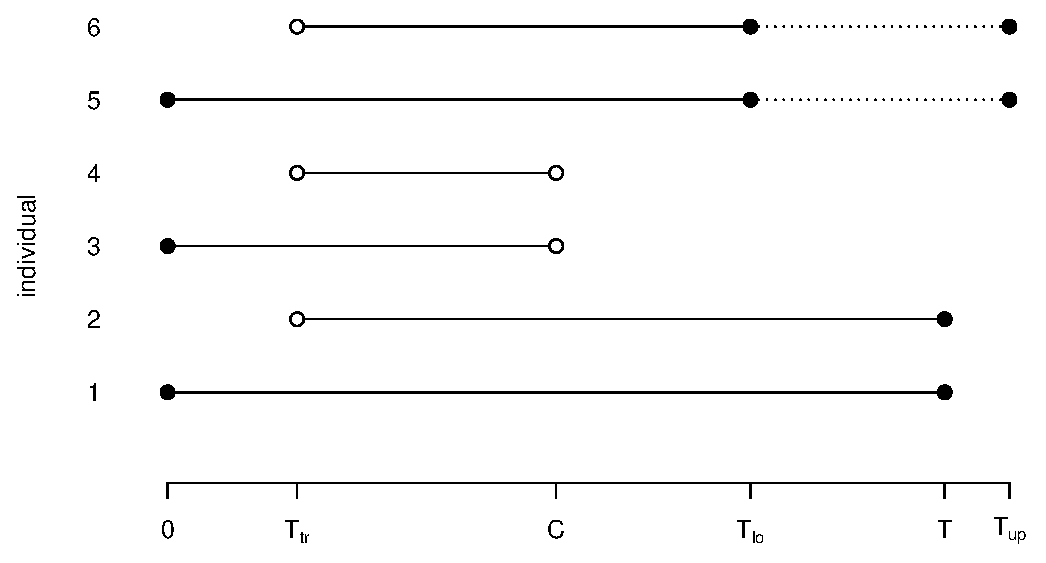
\epsfig{file=grafiken/censoringschemes.eps,scale=0.7}
{\it\caption{Illustration of different censoring
schemes.\label{censoringschemes}}}
\end{center}
\end{figure}

In a general framework an observation can now be uniquely described
 by the quadruple $(T_{tr},T_{lo},T_{up},\delta)$, with
\begin{center}
\begin{tabular}{ll}
$T_{lo}=T_{up}=T$, $\delta=1$ & if the observation is uncensored,\\
$T_{lo}=T_{up}=C$, $\delta=0$ & if the observation is right censored,\\
$T_{lo}<T_{up}$, $\delta=0$ & if the observation is interval censored.\\
\end{tabular}
\end{center}
For left truncated observations we have $T_{tr}>0$ while $T_{tr}=0$
for observations which are not truncated.

Based on these definitions we can now construct the likelihood
contributions for the different censoring schemes in terms of the
hazard rate $\lambda(t)$ and the survivor function
$S(t)=\exp(\int_0^t\lambda(u)du)$. Under the common assumption of
noninformative censoring and conditional independence, the
likelihood is given by
\begin{equation}\label{likelihood}
 L=\prod_{i=1}^n L_i,
\end{equation}
where
\[L_i = \lambda(T_{up})S(T_{up})/S(T_{tr}) = \lambda(T_{up})\exp\left(-\int_{T_{tr}}^{T_{up}}\lambda(t)dt\right)\]
for an uncensored observation,
\[L_i = S(T_{up})/S(T_{tr}) = \exp\left(-\int_{T_{tr}}^{T_{up}}\lambda(t)dt\right)\]
for a right censored observation and
\[L_i = (S(T_{lo})-S(T_{up}))/S(T_{tr}) = \exp\left(-\int_{T_{tr}}^{T_{lo}}\lambda(t)dt\right)\left(1-\exp\left(-\int_{T_{lo}}^{T_{up}}\lambda(t)dt\right)\right)\]
for an interval censored observation. Note that for explicit
evaluation of the likelihood (\ref{likelihood}) some numerical
integration technique has to be employed, since none of the
integrals can in general be solved analytically.

The above notation also allows for the easy inclusion of piecewise
constant, time-varying covariates via some data augmentation. Noting
that
\[\int_{T_{tr}}^{T}\lambda(t)dt = \int_{T_{tr}}^{t_1}\lambda(t)dt + \int_{t_1}^{t_2}\lambda(t)dt + \ldots + \int_{t_{p-1}}^{t_p}\lambda(t)dt + \int_{t_p}^{T}\lambda(t)dt\]
for $T_{tr}<t_1<\ldots<t_q<T$, we can replace an observation
$(T_{tr},T_{lo},T_{up},\delta)$ by a set of new observations
$(T_{tr},t_1,t_1,0)$, $(t_1,t_2,t_2,0)$, \ldots
$(t_{p-1},t_p,t_p,0)$, $(t_{p},T_{lo},T_{up},\delta)$ without
changing the likelihood. Therefore, observations with time-varying
covariates can be split up into several observations, where the
values $t_1<\ldots<t_p$ are defined by the changepoints of the
covariate and the covariate is now time-constant on each of the
intervals. In theory, other paths for a covariate $x(t)$ than
piecewise constant ones are also possible, if $x(t)$ is known for
$T_{tr}\le t\le T_{lo}$. In this case the the likelihood
(\ref{likelihood}) can also be evaluated numerically but a general
path $x(t)$ may lead to complicated data structures.

Figure \ref{timevaryingcovs} illustrates the data augmentation step
for a left truncated, uncensored observation and a covariate $x(t)$
that takes the three different values $x_1,x_2$ and $x_3$ on the
three intervals $[T_{tr},t_1], [t_1,t_2]$ and $[t_2,T_{up}]$. Here,
the original observation $(T_{tr},T_{up},T_{up},1)$ has to be
replaced by $(T_{tr},t_1,t_1,0)$, $(t_1,t_2,t_2,0)$ and
$(t_2,T_{up},T_{up},1)$.
\begin{figure}[htb]
\begin{center}
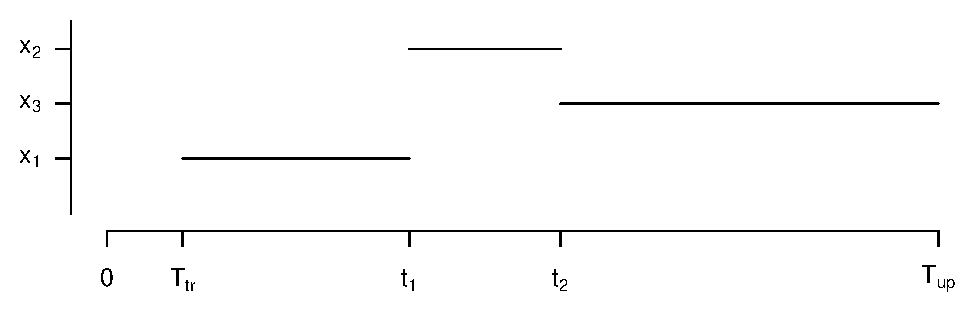
\epsfig{file=grafiken/timevaryingcovs.eps,scale=0.7}
{\it\caption{Illustration of time-varying
covariates.\label{timevaryingcovs}}}
\end{center}
\end{figure}

Currently, interval censored survival times can only be handled with
{\em remlreg objects}.

\subsection{Continuous-time multi-state models}\label{msmodels}
\index{Multi-state models}\index{Recurrent Events}\index{Disease
progression}\index{Competing risks}

Multi-state models are a flexible tool for the analysis of
time-continuous phenomena that can be characterized by a discrete
set of states. Such data structures naturally arise when observing a
discrete response variable for several individuals or objects over
time. Some common examples are depicted in Figure~\ref{some_msms} in
terms of their reachability graph for illustration. For recurrent
events (Figure~\ref{some_msms} (a)), the observations evolve through
time moving repeatedly between a fixed set of states. Other model
classes involve absorbing states, for example disease progression
models (Figure~\ref{some_msms} (b)), that are used to describe the
chronological development of a certain disease. If the severity of
this disease can be grouped into $q-1$ ordered stages of increasing
severity, a reasonable model might look like this: Starting from
disease state '$j$', an individual can only move to contiguous
states, i.e. either the disease gets worse and the individual moves
to state '$j+1$', or the disease attenuates and the individual moves
to state '$j-1$'. In addition, death is included as a further,
absorbing state '$q$', which can be reached from any of the disease
states. A model with several absorbing states is the competing risks
model (Figure~\ref{some_msms} (c)) where, for example, different
causes of death are analysed simultaneously.

\begin{figure}
\begin{center}
 \input{grafiken/msm_examples.tex}
 \caption{Reachability graphs of some common multi-state
 models.\label{some_msms}}
\end{center}
\end{figure}

A multi-state model is fully described by a set of hazard rates
$\lambda_{hi}(t)$ where $h$, $h=1,\ldots,k$, indexes the type of the
transition and $i$, $i=1,\ldots,n$, indexes the individuals. Since
the hazard rates describe durations between transitions, we specify
them in analogy to hazard rate models for continuous time survival
analysis. To be more specific, $\lambda_{hi}(t)$ is modelled in a
multiplicative Cox-type way as
\[
 \lambda_{hi}(t) = \exp(\eta_{hi}(t)),
\]
where
\begin{equation}\label{addpred}
 \eta_{hi}(t) = g_{h0}(t) + \sum_{l=1}^Lg_{hl}(t)u_{il}(t) +
 \sum_{j=1}^Jf_{hj}(x_{ij}(t)) + v_i(t)'\gamma_h +  b_{hi}
\end{equation}
is an additive predictor consisting of the following components:
\begin{itemize}
 \item A time-varying, nonparametric baseline effect $g_{h0}(t)$ common for all
 observations.
 \item Covariates $u_{il}(t)$ with time-varying effects $g_{hl}(t)$.
 \item Nonparametric effects $f_{hj}(x_{ij}(t))$ of continuous covariates
 $x_{ij}(t)$.
 \item Parametric effects $\gamma_h$ of covariates $v_i(t)$.
 \item Frailty terms $b_{hi}$ to account for unobserved
 heterogeneity.
\end{itemize}

For each individual $i$, $i=1,\ldots,n,$ the likelihood contribution
in a multi-state model can be derived from a counting process
representation of the multi-state model. Let $N_{hi}(t)$,
$h=1,\ldots,k$ be a set of counting processes counting transitions
of type $h$ for individual $i$. Consequently, $h=1,\ldots,k$ indexes
the observable transitions in the model under consideration and the
jumps of the counting processes $N_{hi}(t)$ are defined by the
transition times of the corresponding multi-state process for
individual $i$.

From classical counting process theory (see e.g. \citeasnoun{Andetal93}, Ch.~VII.2), the intensity processes $\alpha_{hi}(t)$
of the counting processes $N_{hi}(t)$ are defined as the product of the hazard rate for type $h$ transitions $ \lambda_{hi}(t)$
and a predictable at-risk indicator process $Y_{hi}(t)$, i.e.
\[
 \alpha_{hi}(t) = Y_{hi}(t) \lambda_{hi}(t),
\]
where the hazard rates are constructed in terms of covariates as in
(\ref{addpred}). The at-risk indicator $Y_{hi}(t)$ takes the value
one if individual $i$ is at risk for a type $h$ transition at time
$t$ and zero otherwise. For example, in the multi-state model of
Figure~\ref{some_msms}a), an individual in state 2 is at risk for
both transitions to state 1 and state 3. Hence, the at-risk
indicators for both the transitions '2 to 1' and '2 to 3' will be
equal to one as long as the individual remains in state 2.

Under mild regularity conditions, the individual log-likelihood
contributions can now be obtained from counting process theory as
\begin{equation}\label{loglike1}
 l_i = \sum_{h=1}^k\left[ \int_0^{T_i}\log(\lambda_{hi}(t))dN_{hi}(t) -
 \int_0^{T_i}\lambda_{hi}(t)Y_{hi}(t)dt\right],
\end{equation}
where $T_i$ denotes the time until which individual $i$ has been
observed. The likelihood contributions can be interpreted similarly
as with hazard rate models for survival times (and in fact coincide
with these in the case of a multi-state process with only one
transition to an absorbing state). The first term corresponds to
contributions at the transition times since the integral with
respect to the counting process in fact equals a simple sum over the
transition times. Each of the summands is then given by the
log-intensity for the observed transition evaluated at this
particular time point. In survival models this term simply equals
the log-hazard evaluated at the survival time for uncensored
observations. The second term reflects cumulative intensities
integrated over accordant waiting periods between two successive
transitions. The integral is evaluated for all transitions the
corresponding person is at risk at during the current period. In
survival models there is only one such transition (the transition
from 'alive' to 'dead') and the integral is evaluated from the time
of entrance to the study to the survival or censoring time.

More details on multi-state models, including an exemplary analysis on human sleep, can be found in \citeasnoun{KneHen06}.

\section{Multilevel structured additive distributional and quantile regression}\label{distreg_star}

\subsection{Distributional regression}



Structured additive regression models assume that the distribution of the response variable $y$, given covariates $\xvec$ and $\uvec$, belongs to an exponential family. The conditional mean $\mu_i = E(y_i|\xvec,\uvec)$ is linked to a structured additive predictor
\begin{align*}
\eta_i = f_1(x_{i1}) + \ldots + f_p(x_{ip}) + \uvec_i' \gammavec, \,\,\,\,\,\,\,\, i = 1, \ldots, n,
\end{align*}
by $\mu_i = h(\eta_i)$, see Chapter \ref{obsmodel}. In matrix notation we obtain for the predictor
$$
\etavec = \Xvec_1 \betavec_1 + \ldots + \Xvec_p \betavec_p + \Uvec \gammavec,
$$
see again Chapter \ref{obsmodel} for details.
For the most basic model with Gaussian responses  and the  identity response function we have
\begin{align*}
y_i \sim  \mathcal{N}(\eta_i, \sigma^2) = \mathcal{N}(f_1(x_{i1}) + \ldots + f_p(x_{ip}) + \uvec_i' \gammavec,\sigma^2)
\end{align*}
or
$$
\yvec = \mathcal{N}(\etavec, \sigma^2 \Ivec) = \mathcal{N}(\Xvec_1 \betavec_1 + \ldots + \Xvec_p \betavec_p + \Uvec \gammavec,\sigma^2 \Ivec).
$$


Here and in other convential STAR models only the conditional mean is modeled in dependence of covariates.

A more flexible approach is given by distributional regression as introduced in  \citeasnoun{kleknelan14a} and \citeasnoun{kleknelan14b}. On the one hand, the class of distributions that can be estimated with distributional regression is no longer restricted to the exponential family. On the other hand, distributional regression allows to model not only the conditional mean of the response variable but the whole set of distribution parameters $\varthetavec_1,\ldots,\varthetavec_K$, i.e.~all $K$ parameters of the response distribution can be related to a set of predictor variables, which of course may vary between the different parameters. Using response functions $h_1, \ldots, h_K$ each of these parameters can be linked to a structured additive predictor via
\[
\varthetavec_k = h_k(\etavec_k) = h_k(\Xvec_{1k} \betavec_{1k} + \ldots + \Xvec_{pk} \betavec_{pk} + \Uvec_k \gammavec_k), \quad k=1,\ldots,K.
\]
Usually, the response functions are chosen to ensure appropriate restrictions on the parameter spaces. We use, for example, the exponential function to ensure positivity of the scale parameter.

Presumably the most simple distributional regression model is obtained with Gaussian responses where both the mean $\mu$ and the variance
$\sigma^2$ is modeled in terms of covariates.
Thus, we consider a regression model with
\begin{align*}
\begin{array}{lllll}
\muvec & = & h_1(\etavec_1) & = & \etavec_1, \\ [0.2cm]
\sigmavec^2 & = & h_2(\etavec_2) & = & \exp(\etavec_2).
\end{array}
\end{align*}

A possible generalization of the normal distribution is given by the three-parameter Student's t distribution with location parameter $\mu$, scale parameter $\sigma^2>0$ and degrees of freedom $\texttt{df}>0$. The probability density function is given by
\begin{align*}
f(y|\mu, \sigma, df) = \frac{\Gamma\left( \frac{df +1 }{2}\right)}{\sigma \Gamma\left( \frac{1}{2}\right) \Gamma\left(
\frac{df}{2}\right)\sqrt{df}} \cdot \left( 1+ \frac{(y-\mu)^2}{\sigma^2 df}\right)^{-\frac{df+1}{2}},
\end{align*}
where $\Gamma(x) = \int_0^{\infty} u^{x-1} \exp(-u) \mathrm{d}u$ for $x>0$ is the gamma function. Similar to the normal distribution the t distribution is symmetric and bell-shaped but it has heavier tails, offering a robust alternative to the normal distribution. For $\texttt{df} \rightarrow \infty$ it collapses to the normal distribution.

Regarding the positivity of $\sigma^2$ and $\texttt{df}$ we consider the model
\begin{align*}
\begin{array}{lllll}
\muvec & = & h_1(\etavec_1) & = & \etavec_1, \\ [0.2cm]
\sigmavec^2 & = & h_2(\etavec_2) & = & \exp(\etavec_2), \\ [0.2cm]
\boldsymbol{\texttt{df}} & = & h_3(\etavec_3) & = & \exp(\etavec_3). \\ [0.2cm]
\end{array}
\end{align*}

A popular two parameter distribution for modeling skewed distributions is the gamma distribution with mean parameter $\mu>0$ and shape parameter $\sigma>0$. The probability density function is given by
\begin{equation*}
f(y_i|\mu_i, \sigma_i) = \left( \frac{\sigma_i}{\mu_i} \right)^{\sigma_i} \cdot \frac{y_i^{\sigma_i-1}}{\Gamma(\sigma_i)} \cdot \exp\left(- \frac{\sigma_i}{\mu_i} \cdot y_i \right),
\end{equation*}
The mean of the gamma distribution corresponds to $\mu$, the variance is given by $\mu^2/\sigma$.
Setting up a regression model both the mean and the shape parameter are linked to a STAR predictor via the exponential function due to the positivity constraints:
\begin{align*}
\begin{array}{lllll}
\muvec & = & h_1(\etavec_1) & = & \exp(\etavec_1), \\ [0.2cm]
\sigmavec & = & h_2(\etavec_2) & = & \exp(\etavec_2).
\end{array}
\end{align*}

A comprehensive list of all distributional regression models available in BayesX can be found in Tables \ref{tab:distrBayesX1}  to \ref{tab:distrBayesX4} of the Reference Manual.


\subsection{Quantile Regression} \label{sec:quantreg}

 Distributional regression assumes a specific parametric probability distribution of the response (like the normal, lognormal or gamma distribution) and models some or all of its parameters in dependence of covariates. Quantile regression, in contrast, is a distribution-free approach, trying to directly model the different quantiles of the response as a function of covariates.

In linear quantile regression (see  \citeasnoun{Koe05}), we assume
\begin{align*}
q_{\varphi,i} = \beta_{\varphi,0} + \beta_{\varphi,1}x_{i1} + \ldots + \beta_{\varphi,p}x_{ip}
\end{align*}
where $q_\varphi$, for $\varphi \in (0,1)$, is the $\varphi$-quantile of the response distribution. Estimation of the quantile-specific regression coefficients $\betavec_{\varphi}$ relies on minimizing the asymmetrically weighted error (AWE) criterion
\begin{align}
\hat{\betavec}_{\varphi} = \mbox{argmin}_{\betavec_{\varphi}} \left\{ \sum_{i=1}^{n} \rho_{\varphi}(y_i - \xvec_i' \betavec_{\varphi})\right\},
\label{eq:quantmin}
\end{align}
with the loss function $\rho_{\varphi}$ defined by
\begin{align*}
\rho_{\varphi}(u) = \begin{cases} u \varphi & \textnormal{if $u \geq 0$} \\ u (\varphi - 1) & \textnormal{if $u < 0$,} \end{cases}
\end{align*}
which is also known as the check function. Since there exists no closed form solution for this minimization problem, estimates are typically obtained based on linear programming and modifications of the simplex algorithm, see \citeasnoun{Koe05} for details. The distribution of the response is implicitly determined by the estimated quantiles $q_{\varphi}$ provided that quantiles for a reasonable dense grid of $\varphi$-values are estimated. Generalizations to structured additive predictors are conceptually straightforward. However, estimation is highly challenging and almost impossible for complex hierarchical models, revealing the limits of frequentist quantile regression.

Bayesian structured quantile regression requires a distributional assumption for the responses to be able to set up a likelihood. Following \citeasnoun{WalKneLanYue12} we will assume independent and identically distributed observations following an asymmetric Laplace distribution with location parameter $\eta_{i,\varphi}$ (specified in the usual structured additive fashion), scale parameter $\sigma^2$ and skewness parameter $\varphi$,
\begin{align*}
y_{i} | \eta_{i,\varphi}, \sigma^2, \varphi \overset{\textnormal{iid}}{\sim} \textnormal{ALD}(\eta_{i,\varphi},\sigma^2,\varphi).
\end{align*}
Then, the density of the responses is given by
\begin{align*}
p(y_i | \eta_{i,\varphi},\sigma^2,\varphi) = \frac{\varphi(1-\varphi)}{\sigma^2} \exp\left(-\frac{\rho_{\varphi}(y_i - \eta_i{\varphi})}{\sigma^2}\right).
\end{align*}
Maximizing the corresponding posterior (for fixed $\sigma^2$ and $\varphi$) obviously is equivalent to minimizing the AWE criterion (\ref{eq:quantmin}) in case of a linear predictor. However, in contrast to frequentist quantile regression the linear predictor can be replaced by a hierarchical structured additive predictor without any further difficulties, see \citeasnoun{WalKneLanYue12} for details.

Since the check function $\rho_{\varphi}$ is non-differentiable, inference based on Markov chain Monte Carlo (MCMC) simulations at a first glance seems to be complicated. However, the asymmetric Laplace distribution can be represented as a scaled mixture of normals
\begin{align*}
Y_i = \eta_i + \xi W_i + \delta Z_i \sqrt{\sigma^2 W_i}
\end{align*}
with $\xi = \frac{1-2\varphi}{\varphi(1-\varphi)}$ and $\delta^2 = \frac{2}{\varphi(1-\varphi)}$.  $W_i \sim \textnormal{Exp}(\frac{1}{\sigma^2})$ and $Z_i \sim \mathcal{N}(0,1)$ are independent random variables following an exponential distribution with mean $\sigma^2$ and a standard normal distribution, respectively. Thus, using offsets $\xi W_i$ and weights $\delta \sqrt{\sigma^2 W_i}$ the Bayesian quantile regression problem can be interpreted as a conditionally Gaussian regression model after imputing $W_i$ as a part of the MCMC sampler.


\subsection{Multilevel models}
\label{star_multilevel}

Recently \citeasnoun{LanUml14} have proposed  a multilevel version of STAR models to cope with the hierarchical nature of many data sets.
Suppose that covariate $x_j \in \{1,\dots,K\}$ is a unit- or cluster index   and $x_{ij}$ indicates the cluster
observation $i$ pertains to.
Then the design  matrix $\mathbf{X}_j$ is a $n \times K$ incidence matrix with $\mathbf{X}_j[i,k] = 1$ if the $i$-th observation
belongs to cluster $k$ and zero else. The $K \times 1$ parameter vector $\boldsymbol{\beta}_j$ is the vector of regression parameters,
i.e.~the $k$-th element
in $\boldsymbol{\beta}_j$ corresponds to the regression coefficient of the $k$-th cluster.
We now define a second level equation
\begin{equation}
\label{eq:compprior}
\boldsymbol{\beta}_j = \boldsymbol{\eta}_j + \boldsymbol{\varepsilon}_j =
\mathbf{X}_{j1} \boldsymbol{\beta}_{j1} + \ldots + \mathbf{X}_{jp_j} \boldsymbol{\beta}_{jp_j} +
\mathbf{U}_j \boldsymbol{\gamma}_j +  \boldsymbol{\varepsilon}_j,
\end{equation}
where the terms $\mathbf{X}_{j1} \boldsymbol{\beta}_{j1},\dots,\mathbf{X}_{jp_j} \boldsymbol{\beta}_{jp_j}$ correspond to additional nonlinear
functions $f_{j1},\dots,f_{jp_j}$ and
$\mathbf{U}_j \boldsymbol{\gamma}_j$ comprises additional linear effects of cluster level covariates.
The ``errors'' $\boldsymbol{\varepsilon}_j \sim N(\mathbf{0}, \tau^2_j \mathbf{I})$
comprise a vector of i.i.d.\ Gaussian random effects.
Using the compound prior (\ref{eq:compprior}) we obtain an additive
decomposition of the cluster specific effect. By allowing a full STAR predictor (as in the level-1 equation), a rather complex decomposition of
the cluster effect
$\boldsymbol{\beta}_j$ including interactions is possible. A special case arises if cluster specific covariates are not available. Then the
prior for $\boldsymbol{\beta}_j$ collapses to
$\boldsymbol{\beta}_j = \boldsymbol{\varepsilon}_j \sim N(\mathbf{0}, \tau^2_j \mathbf{I})$ and we obtain a simple i.i.d. Gaussian cluster
specific random effect with variance parameter $\tau^2_j$.

A third or fourth level in the hierarchy is possible by assuming that the second or third level regressions
contain additional cluster-specific random effects whose parameters are again modeled through  STAR predictors of cluster level covariates.



%In a multilevel STAR model (\shortciteN{lanuml14}) the regression coefficients $\betavec_j$ of a function $f_j$ may themselves obey a regression model with a structured additive predictor, i.e.
%\begin{align}
%\betavec_j \sim  \mathcal{N}(\boldsymbol{\eta}_j,\tau^2_j \mathbf{I}) =
%\mathcal{N}(\Zvec_{j1} \betavec_{j1} + \ldots + \Zvec_{jq_j} \betavec_{jq_j} + \Xvec_j \gammavec_j, \tau^2_j \mathbf{I})
%\label{eq:compprior}
%\end{align}
%where the terms $\mathbf{Z}_{j1} \boldsymbol{\beta}_{j1},\dots,\mathbf{Z}_{jq_j} \boldsymbol{\beta}_{jq_j}$ represent additional nonlinear functions $f_{j1},\dots,f_{jq_j}$, and  $\mathbf{X}_j \boldsymbol{\gamma}_j$ comprises additional linear effects.
%Further levels are possible by assuming that the second level regression parameters $\boldsymbol{\beta}_{jl}$, \linebreak $l=1,\dots,q_j$, again obey a STAR model.
%
%In this paper we use the compound prior (\ref{eq:compprior}) if a covariate $z_j \in \{1,\dots,K\}$ is a spatial index and $z_{ij}$ indicates the region observation $i$ pertains to. Then, the design matrix $\mathbf{Z}_j$ is a $n \times K$ incidence matrix with $\mathbf{Z}_j[i,k] = 1$ if the $i$-th observation belongs to region $k$ and zero else. The $K \times 1$ parameter vector $\boldsymbol{\beta}_j$ is the vector of regression parameters, i.e.~the $k$-th element in $\boldsymbol{\beta}$ corresponds to the regression coefficient of the $k$-th region. The use of the compound prior (\ref{eq:compprior}) allows for further explaining the region specific effect by spatial covariates.
%
%The hierarchical structure of the Austrian political-administrative units suggests a four level regression model: Single-family homes (level-1) belong to municipalities (level-2), which are nested in districts (level-3), which are themselves nested in counties (level-4). Assuming house prices per square meter to be normally distributed leads to the following four level STAR model, see also  \shortciteN{brulan11}:
%\begin{align}
%\begin{array}{llll}
%\mbox{level-1:} & \mathit{\boldsymbol{p_{qm}}} &  = & \fvec_1(\mathit{area}) + \fvec_2(\mathit{area\_plot}) + \fvec_3(\mathit{age}) + \fvec_4(\mathit{time\_index}) + \\
%                &              &    & \fvec_5(\mathit{muni}) + \Xvec \gammavec + \varepsilonvec \\
%                &              &  = & \Zvec_1 \betavec_1 + \Zvec_2 \betavec_2 + \Zvec_3 \betavec_3 + \Zvec_4 \betavec_4 + \Zvec_5 \betavec_5 + \Xvec \gammavec + \varepsilonvec  \\ [0.2cm]
%\mbox{level-2:} & \betavec_5   &  = & \fvec_{5,1}(\mathit{pp\_ind}) + \fvec_{5,2}(\mathit{ln\_educ}) +  \fvec_{5,3}(\mathit{age\_ind}) + \fvec_{5,4}(\mathit{comm}) + \\
%                &              &    & \fvec_{5,5}(\mathit{ln\_den}) + \fvec_{5,6}(\mathit{dist}) + \varepsilonvec_5      \\
%                &              &  = & \Zvec_{5,1} \betavec_{5,1} + \Zvec_{5,2} \betavec_{5,2} + \Zvec_{5,3} \betavec_{5,3} + \Zvec_{5,4} \betavec_{5,4} +  \\
%                &              &    & \Zvec_{5,5} \betavec_{5,5} + \Zvec_{5,6} \betavec_{5,6} + \varepsilonvec_5  \\ [0.2cm]
%\mbox{level-3:} & \betavec_{5,6} & = & \fvec_{5,6,1}(\mathit{wko\_ind}) + \fvec_{5,6,2}^{mrf}(\mathit{dist}) + \fvec_{5,6,3}(\mathit{county}) + \varepsilonvec_{5,6} \\
%                &                & = & \Zvec_{5,6,1} \betavec_{5,6,1} + \Zvec_{5,6,2} \betavec_{5,6,2} + \Zvec_{5,6,3} \betavec_{5,6,3} + \varepsilonvec_{5,6} \\ [0.2cm]
%\mbox{level-4:} & \betavec_{5,6,3} & = & \mathds{1} \gamma_0 + \varepsilonvec_{5,6,3}. \\
%\end{array}
%\label{eq:model}
%\end{align}
%
%The categorical covariates on level-1, describing the quality and equipment of the house, are encoded as dummy variables and subsumed in the design matrix $\Xvec$ with estimated parameters $\gammavec$. The possibly nonlinear functions $\fvec_1,\fvec_2,\dots$ are modeled by P-splines.
%
%The level-1 equation contains an uncorrelated random municipality effect $f_5(\emph{muni})$, controlling for unordered spatial heterogeneity. This municipality-specific heterogeneity is modeled through the level-2 equation and is further decomposed into a district and finally into a county level effect (levels 3 and 4). Furthermore, district specific spatial heterogeneity is modeled through a correlated spatial effect $f_{5,6}(\emph{dist})$ in the level-3 equation by Markov random fields, denoted by the superscript "\emph{mrf}", see \shortciteN{fahkne13} for details regarding MRF's.
%
%From model (\ref{eq:model}) we immediately get the conditional mean of the house price per square meter $p_{qm}$. The $\varphi$-th conditional quantile of the house price per square meter is given by
%\begin{equation}
%Q_{\varphi}(p_{qm}) = \EV(p_{qm}) + \sigma \cdot \Phi^{-1}(\varphi),
%\label{eq:quantnormal}
%\end{equation}
%with $\Phi^{-1}(\varphi)$ being the $\varphi$-th quantile of the standard normal distribution. The variance parameter $\sigma^2$ (and so the standard deviation $\sigma$) can be replaced by a suitable estimator.
%%by the sample variance
%%\begin{align*}
%%\widehat{\sigma^2} = S^2 = \frac{\sum_{i=1}^n (p_{qm_i}-\widehat{p_{qm_i}})^2}{n-k},
%%\end{align*}
%%where $k$ denotes the total degrees of freedom.
%Equation (\ref{eq:quantnormal}) shows that the quantiles can be received by simply shifting the mean according to the estimated variance.
%
%Due to the additive structure of our model the conditional quantiles of the house price per square meter change additively with changes in values of covariates. Subsequently, the conditional quantiles of the total house price $p$ change proportionally to the floor area of the building:
%\begin{align*}
%\begin{array}{lll}
%Q_{\varphi}(p) & = & area \cdot \left(\eta + \sigma \cdot \Phi^{-1}(\varphi)\right)\\ [0.2cm]
%     & = & area \cdot \left(f_1(area)+ \ldots + f_5(muni)+\gamma_1 x_1 + \ldots  +\gamma_p x_p + \sigma \cdot \Phi^{-1}(\varphi)\right).
%\end{array}
%\end{align*}
%
%Therefore, if for example covariate $x_1$ changes by one unit, the predictor $\eta$ -- and so the considered quantile of the price per square meter -- changes additively by $\gamma_1$. The quantile of the total price then changes by $area \cdot \gamma_1$. Thus, the change in the quantiles of the price is proportional to the floor area of the building. Turning to the nonlinear effects, let $f(z)$ be the nonlinear effect of a covariate $z$, and let $\mathrm{d}f(z) = f(z+1) - f(z)$. Then, analogously, the quantile of the price per square meter changes by $\mathrm{d}f(z)$ and the quantile of the total price changes by $area \cdot \mathrm{d}f(z)$, again being proportional to the size of the house. Furthermore, since $f(.)$ is a nonlinear function, the change differs over the range of $z$. For the conditional mean we get analog results.
%%\subsubsection*{Lognormally distributed prices}
%%
%%In Section \ref{sec:data} we have seen that the empirical house prices per square meter seem to be approximately lognormally distributed instead of being Gaussian. Assuming the response \emph{$p_{qm}$} to be lognormally distributed, i.e.
%%\begin{align*}
%%\mathit{p_{qm}} \sim \mathcal{LN}(\mu, \sigma^2),
%%\end{align*}
%%leads to normally distributed logged house prices per square meter. Thus, one could guess to improve model (\ref{eq:model}) by replacing the response \emph{$p_{qm}$} by the logged house price per square meter \emph{$lnp_{qm}$}, i.e.
%%\begin{align}
%%\mathit{\boldsymbol{lnp_{qm}}} = \boldsymbol{\eta} + \varepsilonvec,
%%\label{eq:model2}
%%\end{align}
%%which we will call the \emph{Loggaussian model}, with the same hierarchical predictor $\boldsymbol{\eta}$ as before and the errors again being mutually independent normally distributed with mean $0$ and variance $\sigma^2$.
%
%For the loggausian model (\ref{loggaussianm})
%We receive the conditional quantiles of the house price per square meter by
%$$
%\begin{array}{lll}
%Q_{\varphi}(p_{qm}) & = & \exp\left(\eta + \sigma \cdot \Phi^{-1}(\varphi)\right) \\ [0.2cm]
%     & = & \exp\left(f_1(area)+ \ldots + f_5(muni)+\gamma_1 x_1 + \ldots  + \gamma_p x_p + \sigma \cdot \Phi^{-1}(\varphi)\right) \\ [0.2cm]
%     & = & \exp\left(f_1(area)\right) \ldots \exp\left(f_5(muni)\right) \exp(\gamma_1 x_1)  \ldots  \exp(\gamma_p x_p) \exp(\sigma \cdot \Phi^{-1}(\varphi)).
%\end{array}
%$$
%
%Obviously, the conditional quantiles of the house price per square meter $p_{qm}$ now change multiplicatively with changes in values of covariates. If for example covariate $x_1$ changes by one unit, the predictor $\eta$ again changes by $\gamma_1$, but the quantiles of the price per square meter now change multiplicatively by the factor $\exp(\gamma_1)$, yielding
%$$
%\begin{array}{lll}
%\Delta Q_{\varphi}(p_{qm}) & = & \exp(\eta + \sigma \cdot \Phi^{-1}(\varphi)) \cdot \exp(\gamma_1) - \exp(\eta + \sigma \cdot \Phi^{-1}(\varphi))\\ [0.2cm]
%     & = & \exp(\eta + \sigma \cdot \Phi^{-1}(\varphi)) \cdot \left(\exp(\gamma_1)-1\right).
%\end{array}
%$$
%For the conditional quantiles of the total prices we get:
%$$
%\begin{array}{lll}
%Q_{\varphi}(p) & = & area \cdot \exp(\eta + \sigma \cdot \Phi^{-1}(\varphi)) \\ [0.2cm]
%     & = & area \cdot \exp\left(f_1(area)\right) \ldots \exp\left(f_5(muni)\right) \exp(\gamma_1 x_1)  \ldots  \exp(\gamma_p x_p) \exp(\sigma \cdot \Phi^{-1}(\varphi)).
%\end{array}
%$$
%
%So, the quantiles of the total price change multiplicatively with changes in values of covariates too. If for example covariate $x_1$ changes by one unit, the quantiles of the total price change by
%\begin{align*}
%\Delta Q_{\varphi}(p) = area \cdot \exp(\eta + \sigma \cdot \Phi^{-1}(\varphi)) \cdot \left(\exp(\gamma_1)-1\right),
%\end{align*}
%making the change again proportional to the floor area. Similarly, if covariate $z$ (representing a nonlinear effect) changes by one unit, both the conditional quantiles of prices per square meter and the conditional quantiles of total prices multiplicatively change by the factor $\exp\left(\mathrm{d}f(z)\right)$, since
%$$
%\exp\left(f(z+1)\right) = \exp\left(f(z+1)-f(z)+f(z)\right) = \exp\left(\mathrm{d}f(z)\right)\exp\left(f(z)\right).
%$$
%Therefore, the change in the quantiles of total prices caused by a change in any covariate again is proportional to the floor area of the building.
%
%
%For the conditional mean of the house price per square meter
%\begin{align*}
%\EV(p_{qm}) = \exp(\eta + \sigma^2/2)
%\end{align*}
%we get analog results.
%




\addcontentsline{toc}{section}{Bibliography}

\begin{thebibliography}{99}


\harvarditem{Albert \& Chib}{1993}{AlbChi93}
 {\scshape Albert, J. \& Chib, S.} (1993).
 Bayesian Analysis of Binary and Polychotomous Response Data.
 {\it Journal of the American Statistical Association}, {\bf 88}, 669--679.

\harvarditem{Andersen et al.}{1993}{Andetal93}
 {\scshape Andersen, P. K., Borgan, {\O}, Gill, R. D. \& Keiding, N.} (1993).
 {\it Statistical Models Based on Counting Processes.}
 New York: Springer Verlag.

\harvarditem{Andrews \& Mallows}{1974}{AndMal74}
 {\scshape Andrews, D. F. \& Mallows, C. L.} (1974).
 Scale mixtures of Normal Distributions.
 {\it Journal of the Royal Statistical Society B}, {\bf 36}, 99--102.

\harvarditem{Bollaerts, Eilers \& van Mechelen}{2006}{BolEilvMe06}
 {\scshape Albert, J. \& Chib, S.} (1993).
 Simple and Multiple P-Spline Regression with Shape Constraints.
 {\it British Journal of Mathematical and Statistical Psychology}, {\bf 59}, 451--469.

\harvarditem{Belitz}{2007}{Bel07}
 {\scshape Belitz, C.} (2007).
 {\it Model Selection in Generalized Structured Additive Regression Models.}
 PhD Thesis, University of Munich.

\harvarditem{Belitz \& Lang}{2008}{BelLan08}
{\scshape Belitz, C. \& Lang, S.} (2008).
 Simultaneous Selection of Variables and Smoothing Parameters in Structured Additive Regression Models.
{\it Computational Statistics and Data Analysis}, {\bf 53} , 61-81.

\harvarditem{Besag, York \& Molli\'{e}}{1991}{BesYorMol91}
 {\scshape Besag, J., York, J. \& Molli\'{e}, A.} (1991).
 Bayesian Image Restoration with two Applications in Spatial Statistics (with discussion).
 {\it Annals of the Institute of Statistical Mathematics}, {\bf 43}, 1--59.

\harvarditem{Brezger \& Lang}{2006}{BreLan06}
 {\scshape Brezger, A. \& Lang, S.} (2006).
 Generalized Additive Regression based on Bayesian P-Splines.
 {\it Computational Statistics and Data Analysis} {\bf 50}, 967--991.

\harvarditem{Devroye}{1986}{Dev86}
 {\scshape Devroye, L.} (1986).
 {\it Non-Uniform Random Variate Generation.}
 New York: Springer Verlag.

\harvarditem{Eilers \& Marx}{1996}{EilMar96}
 {\scshape Eilers, P. H. C. \& Marx, B. D.} (1996).
 Flexible Smoothing using B-Splines and Penalized Likelihood (with comments and rejoinder).
 {\it Statistical Science}, {\bf 11}, 89--121.

\harvarditem{Fahrmeir, Kneib \& Lang}{2004}{FahKneLan04}
 {\scshape Fahrmeir, L., Kneib, T. \& Lang, S.} (2004).
 Penalized Structured Additive regression for Space-Time Data: A Bayesian Perspective.
 {\it Statistica Sinica}, {\bf 14}, 715--745.

\harvarditem{Fahrmeir et al.}(2013){fahkne13}
{\scshape Fahrmeir, L.,  Kneib, T., Lang, S. \& Marx, B.}{2013}
{\it Regression: Models, Methods and Applications.}
 New York: Springer-Verlag.


\harvarditem{Fahrmeir \& Lang}{2001}{FahLan01a}
 {\scshape Fahrmeir, L. \& Lang, S.} (2001a).
 Bayesian Inference for Generalized Additive Mixed Models Based on Markov Random Field Priors.
 {\it Journal of the Royal Statistical Society C}, {\bf 50}, 201--220.

\harvarditem{Fahrmeir \& Lang}{2001}{FahLan01b}
 {\scshape Fahrmeir, L. \& Lang, S.} (2001b).
 Bayesian Semiparametric Regression Analysis of Multicategorical Time-Space Data.
 {\it Annals of the Institute of Statistical Mathematics}, {\bf 53}, 10--30.

\harvarditem{Fahrmeir \& Osuna}{2006}{FahOsu06}
 {\scshape Fahrmeir, L. \& Osuna, L.} (2006).
 Structured Additive Regression for Overdispersed and Zero-Inflated Count Data.
 {\it Applied Stochastic Models in Business and Industry}, {\bf 22}, 351--369

 \harvarditem{Fahrmeir \& Tutz}{2001}{FahTut01}
 {\scshape Fahrmeir, L. \& Tutz, G.} (2001).
 {\it Multivariate Statistical Modelling based on Generalized Linear Models.}
 New York: Springer-Verlag.

\harvarditem{Fotheringham, Brunsdon \& Charlton}{2002}{FotBruCha02}
 {\scshape Fotheringham, A. S., Brunsdon, C., \& Charlton, M. E.} (2002).
 {\it Geographically Weighted Regression: The Analysis of Spatially Varying Relationships.}
 Chichester: Wiley.

\harvarditem{Gamerman}{1997}{Gam97}
 {\scshape Gamerman, D.} (1997).
 Efficient Sampling from the Posterior Distribution in Generalized Linear Models.
 {\it Statistics and Computing}, {\bf 7}, 57--68.

\harvarditem{Gelfand, Sahu \& Carlin}{1996}{GelSahCar96}
 {\scshape Gelfand, A. E., Sahu, S. K. \& Carlin, B. P.} (1996).
 Efficient Parametrizations for Genera\-lized Linear Mixed Models.
 In: Bernardo, J. M., Berger, J. O., Dawid, A. P. \& Smith, A. F. M. (eds.),
 {\it Bayesian Statistics 5}, 165--180.
 Oxford University Press.

\harvarditem{George \& Liu}{1981}{GeoLiu81}
 {\scshape George, A. \& Liu, J.W.} (1981).
 {\it Computer Solution of Large Sparse Positive Definite Systems.}
 Series in computational mathematics, Prentice-Hall.

\harvarditem{Green}{1987}{Gre87}
 {\scshape Green, P. J.} (1987).
 Penalized Likelihood for General Semiparametric Regression Models.
 {\it International Statistical Review}, {\bf 55}, 245--259.

\harvarditem{Green}{2001}{Gre01}
 {\scshape Green, P. J.} (2001).
 A Primer in Markov Chain Monte Carlo.
 In: Barndorff-Nielsen, O. E., Cox, D. R. \& Kl\"{u}ppelberg, C. (eds.),
 {\it Complex Stochastic Systems}, 1--62.
 Chapmann and Hall, London.

\harvarditem{Green \& Silverman}{1994}{GreSil94}
 {\scshape Green, P. J. \& Silverman, B.} (1994).
 {\it Nonparametric Regression and Generalized Linear Models.}
 Chapman and Hall, London.

\harvarditem{Griffin \& Brown}{2005}{GriBro05}
 {\scshape Griffin, J. E., and Brown, P. J.} (2005). Alternative Prior Distributions
 for Variable Selection with very many more Variables than Observations. Technical
 report, University of Warwick, Dept. of Statistics.

\harvarditem{Harville}{1977}{Har77}
 {\scshape Harville, D. A.} (1977).
 Maximum Likelihood Approaches to Variance Component Estimation and to related Problems.
 {\it Journal of the American Statistical Association}, {\bf 72}, 320--338.

\harvarditem{Hastie \& Tibshirani}{1990}{HasTib90}
 {\scshape Hastie, T. \& Tibshirani, R.} (1990).
 {\it Generalized Additive Models.}
 Chapman and Hall, London.

\harvarditem{Hastie \& Tibshirani}{1993}{HasTib93}
 {\scshape Hastie, T. \& Tibshirani, R.} (1993).
 Varying-Coefficient Models.
 {\it Journal of the Royal Statistical Society B}, {\bf 55}, 757--796.

\harvarditem{Hastie \& Tibshirani}{2000}{HasTib00}
 {\scshape Hastie, T. \& Tibshirani, R.} (2000).
 Bayesian Backfitting.
 {\it Statistical Science}, {\bf 15}, 193--223.

\harvarditem{Hastie, Tibshirani \& Firedman}{2001}{HasTibFri01}
 {\scshape Hastie, T., Tisbshirani, R. \& Friedman, J.} (2001).
 {\it The Elements of Statistical Learning: Data Mining, Inference and Prediction.}
 New York: Springer-Verlag.

\harvarditem{Hennerfeind, Brezger \& Fahrmeir}{2006}{HenBreFah06}
 {\scshape Hennerfeind, A., Brezger, A. \& Fahrmeir, L.} (2006).
 Geoadditive Survival Models.
 {\it Journal of the American Statistical Association}, {\bf 101}, 1065--1075.

\harvarditem{Holmes \& Held}{2006}{HolHel06}
 {\scshape Holmes, C., Held, L.} (2006).
 Bayesian Auxiliary Variable Models for Binary and Multinomial Regression.
 {\it Bayesian Analysis}, {\bf 1}, 145--168.

\harvarditem{Hurvich, Simonoff \& Tsai}{1998}{HurSimTsa98}
 {\scshape Hurvich, C. M., Simonoff, J. S. \& Tsai, C. L.} (1998).
 Smoothing Parameter Selection in Nonparametric Regression using an improved {A}kaike Information Criterion.
 {\it Journal of the Royal Statistical Society B}, {\bf 60}, 271--293.

\harvarditem{Ishwaran \& Rao}{2005}{IshRao05}
 {\scshape Ishwaran, H., and Rao, S. J.} (2005). Spike and Slab Variable
 Selection: Frequentist and Bayesian Strategies. {\it The Annals of Statistics},
 {\bf 33}, 730-773.

\harvarditem{Johnson, Moore \& Ylvisaker}{1990}{JohMooYlv90}
 {\scshape Johnson, M.E., Moore, L.M. \& Ylvisaker, D.} (1990).
 Minimax and Maximin Designs.
 {\it Journal of Statistical Planning and Inference}, {\bf 26}, 131--148.

\harvarditem{Kammann \& Wand}{2003}{KamWan03}
 {\scshape Kammann, E. E. \& Wand, M. P.} (2003).
 Geoadditive Models.
 {\it Journal of the Royal Statistical Society C}, {\bf 52}, 1--18.


\harvarditem{Klein et al.}{2014a}{KleDenKneLan14}
{\scshape Klein, N., Denuit, M., Kneib, T. \& Lang, S.}(2014).
Nonlife Ratemaking and Risk Management with Bayesian additive Models for Location, Scale and Shape.
{\it Insurance: Mathematics and Economics}, {\bf 55}, 225--249.


\harvarditem{Klein et al.}{2014b}{kleknelan14a}
{\scshape Klein, N., Kneib, T., Lang, S.}(2013).
Bayesian Structured Additive Distributional Regression.
{\it Under revision for Annals of Applied Statistics}.


\harvarditem{Klein, Kneib \& Lang}{2014}{kleknelan14b}
{\scshape Klein, N., Kneib, T. \& Lang, S.}(2014).
Bayesian Generalized Additive Models for Location, Scale and Shape for Zero-Inflated and Overdispersed Count Data.
To appear in {\it Journal of the American Statistical Association}, doi:10.1080/01621459.2014.912955.


\harvarditem{Klein et al.}{2014c}{KleKneLan14c}
{\scshape Klein, N., Kneib, T., Klasen, S. \& Lang, S.}(2014).
Bayesian Structured Additive Distributional Regression for Multivariate Responses.
To appear in {\it Journal of the Royal Statistical Society C}, doi:10.1111/rssc.12090.


\harvarditem{Koenker}{2005}{Koe05}
{\scshape Koenker, R.}(2005).
{\it Quantile Regression.}
Cambridge University Press, New York.



\harvarditem{Kneib}{2006}{Kne06}
 {\scshape Kneib, T.} (2006).
 Geoadditive Hazard Regression for Interval Censored Survival Times.
 {\it Computational Statistics and Data Analysis}, {\bf 51}, 777--792

\harvarditem{Kneib \& Hennerfeind}{2006}{KneHen06}
 {\scshape Kneib, T. \& Hennerfeind, A.} (2006).
 Bayesian Semiparametric Multi-State Models.
 {\it Statistical Modelling}, {\bf 8}, 169--198.

\harvarditem{Kneib \& Fahrmeir}{2006}{KneFah06}
 {\scshape Kneib, T. \& Fahrmeir, L.} (2006).
 Structured Additive Regression for Categorical Space-Time Data: A Mixed Model approach.
 {\it Biometrics}, {\bf 62}, 109--118.

\harvarditem{Kneib \& Fahrmeir}{2007}{KneFah07}
 {\scshape Kneib, T. \& Fahrmeir, L.} (2007).
 A Mixed Model Approach to Structured Hazard Regression.
 {\it Scandinavian Journal of Statistics}, {\bf 34}, 207--228.

\harvarditem{Kneib et al.}{2009}{Kne09}
 {\scshape Kneib, T., Konrath, S. und Fahrmeir, L.} (2009). High-dimensional
 Structured Additive Regression Models: Bayesian Regularisation, Smoothing and Predictive
 Performance. Department of Statistics, Technical Report No. 46, LMU Munich.

\harvarditem{Knorr-Held}{1999}{KnoHel99}
 {\scshape Knorr-Held, L.} (1999).
 Conditional Prior Proposals in Dynamic Models.
 {\it Scandinavian Journal of Statistics}, {\bf 26}, 129--144.

\harvarditem{Konrath et al.}{2008}{Kon08}
 {\scshape Konrath, S., Kneib, T., Fahrmeir, L.} (2008). Bayesian Regularisation
 in Structured Additive Regression Models for Survival Data. Department of Statistics,
 Technical Report No.35, LMU Munich.

\harvarditem{Lang \& Brezger}{2004}{LanBre04}
 {\scshape Lang, S. \& Brezger, A.} (2004).
 Bayesian P-Splines.
 {\it Journal of Computational and Graphical Statistics}, {\bf 13}, 183--212.

\harvarditem{Lang et al.}{2014}{LanUml14}
 {\scshape Lang, S., Umlauf, N., Wechselberger, P., Harttgen, K.  \& Kneib, T.} (2014).
 Multilevel Structured Additive Regression.
 {\it Statistics and Computing}, {\bf 24}, 223--238.


\harvarditem{Lin \& Zhang}{1999}{LinZha99}
 {\scshape Lin, X. \& Zhang, D.} (1999).
 Inference in Generalized Additive Mixed Models by using Smoothing Splines.
 {\it Journal of the Royal Statistical Society B}, {\bf 61}, 381--400.

\harvarditem{McCullagh \& Nelder}{1989}{McCNel89}
 {\scshape McCullagh, P. \& Nelder, J. A.} (1989).
 {\it Generalized Linear Models.}
 Chapman and Hall, London.

\harvarditem{M\"{u}ller, Stadtm\"{u}ller \& Tabnak}{1997}{MueStaTab97}
 {\scshape M\"{u}ller, H. G., Stadtm\"{u}ller, U. \& Tabnak, F.} (1997).
 Spatial Smoothing of Geographically Aggregated Data, with Applications to the Construction of Incidence Maps.
 {\it Journal of the American Statistical Association} {\bf 92}, 61--71.

\harvarditem{Nychka \& Saltzman}{1998}{NycSal98}
 {\scshape Nychka, D. \& Saltzman, N.} (1998).
 {\it Design of Air-Quality Monitoring Networks.}
 Lecture Notes in Statistics, 132, 51--76.

\harvarditem{Osuna}{2004}{Osu04}
 {\scshape Osuna, L.} (2004)
 {\it Semiparametric Bayesian Count Data Models}.
 Dr. Hut Verlag, M\"{u}nchen.

\harvarditem{Park \& Casella}{2008}{ParCas08}
 {\scshape Park, T., and Casella, G.} (2008). The Bayesian Lasso.
 {\it Journal of the American Statistical Association}, {\bf 482}, 681-686.

\harvarditem{Rue}{2001}{Rue01}
 {\scshape Rue, H.} (2001).
 Fast Sampling of Gaussian Markov Random Fields with Applications.
 {\it Journal of the Royal Statistical Society B}, {\bf 63}, 325--338.

\harvarditem{Ruppert, Wand \& Carroll}{2003}{RupWanCar03}
 {\scshape Ruppert, D., Wand, M. P. \& Carroll, R. J.} (2003).
 {\it Semiparametric Regression.}
 Cambridge University Press.

\harvarditem{Spiegelhalter et al.}{2002}{SpiBesCar02}
 {\scshape Spiegelhalter, D. J., Best, N. G., Carlin, B. P. \& van der Linde, A.} (2002).
 Bayesian Measures of Model Complexity and Fit.
 {\it Journal of the Royal Statistical Society B}, {\bf 65}, 583--639.

\harvarditem {Waldmann et al.}{2013}{WalKneLanYue12}
{\scshape Waldmann, E. and Kneib, T. and Lang, S. and Yue, Y.}(2013)
Bayesian Semiparametric Additive  Quantile Regression.
{\it Statistical Modelling}, {\bf 13}, 223--252.



\end{thebibliography}

\addcontentsline{toc}{section}{Index}
\input{manual_star.ind}
\hypertarget{index}{}

\end{document}

\hypertarget{index}{}

\end{document}

\hypertarget{index}{}

\end{document}


\chapter{bayesreg objects}
\label{bayesreg} \index{bayesreg object}

{\em Authors: Andreas Brezger, Stefan Lang and Thomas Kneib} \\
{\em email:
\href{mailto:andib@stat.uni-muenchen.de}{andib@stat.uni-muenchen.de},
\href{mailto:lang@stat.uni-muenchen.de}{lang@stat.uni-muenchen.de}}
and
\href{mailto:kneib@stat.uni-muenchen.de}{kneib@stat.uni-muenchen.de} \\
\vspace{0.3cm}


{\em bayesreg objects} are used to fit (multivariate) generalized
linear models or hazard rate models with a {\em Structured
Additive Predictor (STAR)}, see Fahrmeir, Kneib, and Lang (2003).
Inference is fully Bayesian via Markov Chain Monte Carlo (MCMC)
techniques. The methodological background is provided in
considerable detail in \autoref{star}. More details can be found
in Fahrmeir and Lang (2001a), Fahrmeir and Lang (2001b), Lang and
Brezger (2003), Brezger and Lang (2003), Fahrmeir and Osuna
(2003), Hennerfeind, Brezger and Fahrmeir (2003), and Fahrmeir and
Hennerfeind (2003). Good introductions into generalized linear
models are the monographs of Fahrmeir and Tutz (2001) and Mc
Cullagh and Nelder (1989). Introductions to semi- and
nonparametric models are given in Green and Silverman (1994),
Hastie and Tibshirani (1990), Hastie and Tibshirani (1993) and
Hastie, Tibshirani and Friedman (2001). The paper of Chib and
Greenberg (1995), the monograph {\em Markov Chain Monte Carlo in
Practice} edited by Gilks, Richardson and Spiegelhalter (1996) and
the article by Green (2001) give a good overview over MCMC
simulation techniques.

First steps with {\em bayesreg objects} can be done with the
tutorial like examples in \autoref{bayesregexamples}.


\section{Method regress}
\label{bayesregress} \index{bayesreg object!regress command}


\subsection{Description}
\label{bayesregregressdescr}

Method #regress# estimates regression or hazard rate models with
Structured Additive Predictor. An introduction to the
methodological background can be found in \autoref{star}.

\index{generalized linear models} \index{generalized additive
models} \index{varying coefficients models} \index{Bayesian
semiparametric regression} \index{MCMC} \index{Markov chain Monte
Carlo}



\subsection{Syntax}
\label{bayesregregresssyntax}

 #>#{\em objectname}.#regress# {\em model} [#weight# {\em weightvar}] [#if# {\em expression}] [{\em , options}] #using# {\em dataset}

Method #regress# estimates the regression model specified in {\em
model} using the data specified in {\em dataset}. {\em dataset}
must be the name of a {\em dataset object} created before. The
details of correct models are covered in \autoref{modelsyntax}.
The distribution of the response variable can be either Gaussian,
gamma, binomial, multinomial, Poisson or negative binomial, see
also \autoref{familyopt} for an overview about the distributions
supported by {\em BayesX}. The response distribution is specified
using option #family#, see \autoref{familysyntax} below and the
options list in \autoref{regressoptions} for a detailed
description. The default is #family=binomial# with a logit link.
An #if# statement may be specified to analyze only a part of the
data set, i.e.~the observations where {\em expression} is true.

\subsubsection{Optional weight variable }
\label{weightspecification}

An optional weight variable {\em weightvar} may be specified to
estimate weighted regression models. For Gaussian responses {\em
BayesX} assumes that $y_r|\eta_r,\sigma^2 \sim
N(\eta,\sigma^2/weightvar_r)$. Thus, for grouped Gaussian
responses the weights must be the number of observations in the
groups if the $y_r$'s are the average of individual responses. If
the $y_r$'s are the sum of responses in every group, the weights
must be the reciprocal of the number of observations in the
groups. Of course, estimation of usual weighted regression models
with heteroscedastic errors  is also possible. In this case the
weights should be proportional to the reciprocal of the
heteroscedastic variances. If the response distribution is
binomial, it is assumed that the values of the weight variable
correspond to the number of replications and that the values of
the response variable correspond to the number of successes. If
#weight# is omitted, {\em BayesX} assumes that the number of
replications is one, i.e.~the values of the response must be
either zero or one. For grouped Poisson data the weights must be
the number of observations in a group and the $y_i$'s are assumed
to be the average of individual responses. In the case of gamma
distributed responses {\em BayesX} assumes $y_r \sim
G(\exp(\eta_r),\nu/weightvar_r)$ where $\mu_r= \exp(\eta_r)$ is
the mean and $s_r = \nu/weightvar_r$ is the scale parameter.

If estimation is based on latent utility representations, the
specification of weights is not allowed. Also for negative
binomial models weighted regression is not implemented.

\subsubsection{Syntax of possible model terms}
\label{modelsyntax}

The general syntax of models is:

$depvar = term_1 + term_2 + \cdots + term_r$

{\em depvar} specifies the dependent variable in the model and
$term_1$,\dots,$term_r$ define in which way the covariates
influence the dependent variable. The different terms must be
separated by '+' signs. A constant intercept is automatically
included in the models and must not be specified by the user. This
section reviews all possible model terms that are supported in the
current version of {\em bayesreg objects} and provides some
specific examples. Note that all described terms may be combined
in arbitrary order. An overview about the capabilities of {\em
bayesreg objects} is given in \autoref{terms}.
\autoref{bayesreginteractions} shows how interactions between
covariates are specified. Full details about all available options
are given in \autoref{localoptions}.

Throughout this section #Y# denotes the dependent variable.

{\bf Offset}
\medskip

\begin{itemize}
\item[] {\em Description}: Adds an offset term to the predictor.
\item[] {\em Predictor}: $\eta =  \cdots + offs + \cdots$
\item[] {\em Syntax}: #offs(offset)#
\item[] {\em Example}:

For example, the following model statement can be used to estimate
a Poisson model with #offs# as offset term and #W1# and #W2# as
fixed effects (if #family=poisson# is specified in addition):

\texttt{Y = offs(offset) + W1 + W2}

\end{itemize}

\newpage

{\bf Fixed effects}
\medskip

\begin{itemize}
\item[] {\em Description}: Incorporates covariate #W1# as a fixed effect into the model.
\item[] {\em Predictor}: $\eta =  \cdots + \gamma_1 W1 + \cdots$
\item[] {\em Syntax}: #W1#
\item[] {\em Example}:

The following model statement causes {\em BayesX} to estimate a
model with $q$ fixed (linear) effects:

\texttt{Y = W1 + W2 + $\cdots$ + Wq}
\end{itemize}


{\bf Nonlinear effects of continuous covariates and time scales}
\medskip

{\em First or second order random walk}

\begin{itemize}
\item[] {\em Description}: Defines a first or second order random walk prior for the effect of #X1#.
\item[] {\em Predictor}: $\eta = \cdots + f_1(X1) + \cdots $
\item[] {\em Syntax}:

#X1(rw1#[, {\em options}]#) #

#X1(rw2#[, {\em options}]#) #
\item[] {\em Example}:

Suppose we have a continuous covariate #X1#, whose effect is
assumed to be nonlinear. The following model statement defines a
second order random walk prior for $f_1$:

#Y = X1(rw2,a=0.001,b=0.001)#

Here, the expression #X1(rw2,a=0.001,b=0.001)# indicates, that the
effect of #X1# should be incorporated nonparametrically into the
model using a second order random walk prior. A first order random
walk is specified in the model statement by modifying the first
argument in #X1(rw2,a=0.001,b=0.001)# from #rw2# to #rw1# which
yields the term #X1(rw1,a=0.001,b=0.001)#. The second and third
argument in the expression above are used to specify the
hyperparameters of the inverse gamma prior for the variance.
Besides the options #a# and #b# some more options are available,
see \autoref{localoptions} for details.
\end{itemize}

\vspace{0.5cm}

{\em P-spline with first or second order random walk penalty}

\begin{itemize}
\item[] {\em Description}: Defines a P-spline with a first or second order random walk penalty for
the parameters of the spline.
\item[] {\em Predictor}: $\eta =  \cdots + f_1(X1) + \cdots$
\item[] {\em Syntax}:

#X1(psplinerw1#[{\em , options}]#) #

#X1(psplinerw2#[{\em , options}]#) #
\item[] {\em Example}:

For example, a P-spline with second order random walk penalty is
obtained using the following model statement:

#Y = X1(psplinerw2)#

By default, the degree of the spline is 3 and the number of inner
knots is 20. The following model term defines a quadratic P-spline
with 30 knots:

#Y = X1(psplinerw2,degree=2,nrknots=30)#

Full details about all possible options for P-splines are given in
\autoref{localoptions}.
\end{itemize}


{\em Seasonal component for time scales}

\begin{itemize}
\item[] {\em Description}: Defines a seasonal effect of #time#.
\item[] {\em Predictor}: $\eta =  \cdots + f_{season}(time) + \cdots $
\item[] {\em Syntax}:

#time(season#[, {\em options}]#) #
\item[] {\em Example}:

A seasonal component for a time scale #time# is specified for
example by

#Y = time(season,period=12)#.

Here, the second argument specifies the period of the seasonal
effect. In the example above the period is 12, corresponding to
monthly data.
\end{itemize}


{\bf Spatial Covariates}
\medskip

{\em Markov random field}

\begin{itemize}
\item[] {\em Description}:

Defines a Markov random field prior for the spatial covariate
#region#. {\em BayesX} allows an appropriate incorporation of
spatial covariates using one of the Markov random field priors
(\ref{adjacency}) or (\ref{intrinsic}) with geographical
information stored in the {\em map object} specified through the
option #map#.
\item[] {\em Predictor}: $\eta = \cdots + f_{spat}(region) + \cdots$
\item[] {\em Syntax}:

#region(spatial,map=#{\em characterstring}#[#{\em , options}]#) #
\item[] {\em Example}:

The specification of a Markov random field prior for spatial data
has #map# as a required argument which must be the name of a {\em
map object} (see \autoref{map}) that contains all necessary
spatial information about the geographical map, i.e.~the neighbors
of each region and the weights associated with the neighbors. For
example the statement

#Y = region(spatial,map=germany)#

defines a Markov random field prior for #region# where the
geographical information is stored in the {\em map object}
#germany#. An error will be raised if #germany# is not existing.
It is advisable to reorder the regions of a map in advance to
obtain a band matrix like precision matrix. This is achieved using
method #reorder# of {\em map objects}, see \autoref{mapreorder}
for details.
\end{itemize}



{\em 2 dimensional P-spline with first order random walk penalty}

\begin{itemize}
\item[] {\em Description}:

Defines a 2 dimensional P-spline for the spatial covariate
#region# based on the tensor product of 1 dimensional P-splines
with a 2 dimensional first order random walk penalty for the
parameters of the spline. Estimation is based on the coordinates
of the centroids of the regions an observation pertains to. The
centroids are computed using the geographical information stored
in the {\em map object} specified through the option #map#.
\item[] {\em Predictor}: $\eta= \cdots + f(centroids) + \cdots$
\item[] {\em Syntax}:

#region(geospline,map=#{\em characterstring}#[, #{\em options}]#) #
\item[] {\em Example}:

The specification of a 2 dimensional P-spline ({\em geospline})
for spatial data has #map# as a required argument which must be
the name of a {\em map object} (see \autoref{map}) that contains
all necessary spatial information about the geographical map,
i.e.~the neighbors of each region and the weights associated with
the neighbors. The model term

#Y = region(geospline,map=germany)#

specifies a tensor product cubic P-spline with first order random
walk penalty where the geographical information is stored in the
{\em map object} #germany#.
\end{itemize}

\vspace{0.5cm}

{\bf Unordered group indicators}
\medskip

{\em Unit- or cluster specific unstructured effect}

\begin{itemize}
\item[] {\em Description}: Defines an unstructured (uncorrelated) random effect with respect
to grouping variable #grvar#.
\item[] {\em Predictor}: $\eta = \cdots + f(grvar) + \cdots$
\item[] {\em Syntax}:

#grvar(random#[, {\em options}]#) #
\item[] {\em Example}:

{\em BayesX} also supports Gaussian i.i.d.~random effects to cope
with unobserved heterogeneity among units or clusters of
observations. Suppose the analyzed data set contains a group
indicator #grvar# that gives information about the individual or
cluster a particular observation belongs to. Then an individual
specific uncorrelated random effect is incorporated through the
term

#Y = grvar(random)#

The inclusion of more than one random effects term in the model is
possible allowing the estimation of multilevel models. However, we
have only limited experience with multilevel models so that it is
not clear how well these models can be estimated in {\em BayesX}.
\end{itemize}

\newpage

{\bf Nonlinear baseline effect in Cox models}
\medskip

{\em P-spline with second order random walk penalty}

\begin{itemize}
\item[] {\em Description}: Defines a P-spline with a second order random walk penalty for the
parameters of the spline for the log-baseline effect
$\log(\lambda_0$(#time#)).
\item[] {\em Predictor}: $\eta = \log(\lambda_0(time)) + \cdots$
\item[] {\em Syntax}:

#time(baseline#[, {\em options}]#) #
\item[] {\em Example}:

Suppose continuous-time survival data (#time#, #delta#) together
with additional covariates (#W1#,#X1#) are given where #time#
denotes the vector of observed duration times, #delta# is the
vector of corresponding indicators of non-censoring, #W1# is a
discrete covariate and #X1# a continuous one. The following Cox
model with hazard rate $\lambda$ and log-baseline effect
$\log(\lambda_0$(#time#))
\[
\lambda(time)=\lambda_0(time)\exp (\gamma_0 + \gamma_1 W1 + f(X1)
)=\exp\left(\log(\lambda_0(time)) + \gamma_0 + \gamma_1 W1 +
f(X1)\right)
\]
is estimated by the model statement

#delta = time(baseline) + W1 + X1(psplinerw2)#

Note that a baseline term has to be specified in the model.
\end{itemize}


{\bf Varying coefficients with continuous covariates as effect
modifier}
\medskip

{\em First or second order random walk}

\begin{itemize}
\item[] {\em Description}:

Defines a varying coefficient term, where the effect of #X1#
varies smoothly over the range of #X2#. Covariate #X2# is the
effect modifier. The smoothness prior for $f$ is a first or second
order random walk.
\item[] {\em Predictor}: $\eta= \cdots + f(X2)X1 + \cdots$
\item[] {\em Syntax}:

#X1*X2(rw1#[, {\em options}]#) #

#X1*X2(rw2#[, {\em options}]#) #
\item[] {\em Example}:

For example, a varying coefficient term with a second order random
walk smoothness prior is defined as follows:

#Y = X1*X2(rw2)#
\end{itemize}


{\em P-spline with first or second order random walk penalty}
\begin{itemize}
\item[] {\em Description}:

Defines a varying coefficient term, where the effect of #X1#
varies smoothly over the range of #X2#. Covariate #X2# is the
effect modifier. The smoothness prior for $f$ is a P-spline with
first or second order random walk penalty.
\item[] {\em Predictor}: $\eta= \cdots + f(X2)X1 + \cdots$
\item[] {\em Syntax}:

#X1*X2(psplinerw1#[, {\em options}]#) #

#X1*X2(psplinerw2#[, {\em options}]#) #
\item[] {\em Example}:

For example, a varying coefficient term with a second order random
walk smoothness prior is defined as follows:

#Y = X1*X2(psplinerw2)#

\end{itemize}


{\em Seasonal prior}
\begin{itemize}
\item[] {\em Description}:

Defines a varying coefficients term where the effect of #X1#
varies over the range of the effect modifier #time#. For #time#
the seasonal prior (\ref{seasonal}) is used.
\item[] {\em Predictor}: $\eta= \cdots + f_{season}(time)X1 + \cdots $
\item[] {\em Syntax}:

#X1*time(season#[, {\em options}]#) #
\item[] {\em Example}:

The inclusion of a varying coefficients term with a seasonal prior
may be meaningful if we expect a different seasonal effect with
respect to grouping variable #X1#. In this case we can include
additional seasonal effects for each category of #X1# by

#Y = X1*time(season) #

\end{itemize}

{\bf Time-varying effects in Cox models}
\medskip

{\em P-spline with second order random walk penalty}

\begin{itemize}
\item[] {\em Description}: Defines a varying coefficients term
where the effect of #X1# varies over the range of the effect
modifier #time#, i.e. variable #X1# has time-varying effect. The
smoothness prior for $f($#time#$)$ is a P-spline with second order
random walk penalty.

 \item[] {\em Predictor}: $\eta = \log(\lambda_0(time)) +
f(time)X1 \cdots$ \item[] {\em Syntax}:

 #X1*time(baseline#[, {\em options}]#) #
 \item[] {\em Example}:

Suppose continuous-time survival data (#time#, #delta#) together
with an additional covariate #X1# are given, where #time# denotes
the vector of observed duration times, #delta# is the vector of
corresponding indicators of non-censoring. The following Cox model
with hazard rate $\lambda$
\begin{eqnarray*}
 \lambda(time) & = & \lambda_0(time)\exp(\gamma_0 + f(time)X1)\\
 & = & \exp\left(\log(\lambda_0(time)) + \gamma_0 + f(time)X1\right)
\end{eqnarray*}
is estimated by the model statement

#delta = time(baseline) + X1*time(baseline)#

\end{itemize}


{\bf Varying coefficients with spatial covariates as effect
modifiers} \medskip

{\em Markov random field}

\begin{itemize}
\item[] {\em Description}:

Defines a varying coefficient term where the effect of #X1# varies
smoothly over the range of the spatial covariate #region#. A
Markov random field is estimated for $f_{spat}$. The geographical
information is stored in the {\em map object} specified through
the option #map#.
\item[] {\em Predictor}: $\eta = \cdots + f_{spat}(region)X1 + \cdots$
\item[] {\em Syntax}:

#X1*region(spatial,map=#{\em characterstring}#[,#{\em options}]#) #
\item[] {\em Example}:

For example the statement

#Y = X1*region(spatial,map=germany) #

defines a varying coefficient term with the spatial covariate
#region# as the effect modifier and the spatial smoothness prior
(\ref{adjacency}), or the more general prior (\ref{intrinsic})
depending on the weight definition in the {\em map object}
#germany#.
\end{itemize}


%{\em 2 dimensional P-spline with first order random walk penalty}
%\begin{itemize}
%\item[] {\em Description}:

%Defines a varying coefficients term where the effect of X1 varies
%smoothly over the range of the spatial covariate X2. A 2
%dimensional P-spline based on the tensor product of 1 dimensional
%P-splines with a 2 dimensional first order random walk penalty for
%the parameters of the spline is estimated for $f$. The centroids
%are computed using the geographical information stored in the map
%object specified through the option #map#.
%\item[] {\em Predictor}: $\eta= \cdots + f(centroids)X1 + \cdots$
%\item[] {\em Syntax}:

%X1*X2(geospline,map=characterstring[, options])
%\item[] {\em Example}:
%\end{itemize}


{\bf Varying coefficients with unordered group indicators as effect modifiers \\
(random slopes)}
\medskip

{\em Unit- or cluster specific unstructured effect}
\begin{itemize}
\item[] {\em Description}:

Defines a varying coefficient term where the effect of #X1# varies
over the range of the group indicator #grvar#. Models of this type
are usually referred to as random slope models. A  Gaussian
i.i.d.~random effect with respect to grouping variable #grvar# is
assumed for $f$. A main effect $\gamma X1$ is additionally
estimated using a diffuse prior for $\gamma$. This means that the
random slope effect $f(grvar)X1$ can be seen as the deviation from
the main effect. Estimation is carried out using hierarchical
centering, see Gelfand, Sahu and Carlin (1995). Note that
nonsensical results are obtained if an additional fixed effect of
#X1# is added in the model statement because the fixed effect is
automatically estimated.
\item[] {\em Predictor}: $\eta = \cdots + \gamma X1 + f(grvar)X1 + \cdots$
\item[] {\em Syntax}:

#X1*grvar(random#[, {\em options}]#) #
\item[] {\em Example}:

For example, a random intercept term with incorporation of #X1# as
fixed effect is specified as follows:

#Y = X1*grvar(random)#

If the linear effect of #X1# should be omitted, the option
#nofixed# must be specified:

#Y = X1*grvar(random,nofixed)#
\end{itemize}


{\bf Surface estimators}
\medskip

{\em 2 dimensional P-spline with first order random walk penalty}
\begin{itemize}
\item[] {\em Description}:

Defines a 2 dimensional P-spline based on the tensor product of 1
dimensional P-splines with a 2 dimensional first order random walk
penalty for the parameters of the spline.
\item[] {\em Predictor}: $\eta= \cdots + f(X1,X2) + \cdots$
\item[] {\em Syntax}:

#X1*X2(pspline2dimrw1#[, {\em options}]#) #
\item[] {\em Example}:

The model term

#Y = X1*X2(pspline2dimrw1)#

specifies a tensor product cubic P-spline with first order random
walk penalty.

In many applications it is favorable to additionally incorporate
the 1 dimensional main effects of #X1# and #X2# into the models.
In this case the 2 dimensional surface can be seen as the
deviation from the main effects. Note, that the number of inner
knots has to be the same for the main effects and the interaction
effect. For example, splines with 10 inner knots are estimated by


 #Y = X1(psplinerw2,nrknots=10) + X2(psplinerw2,nrknots=10)#\\
 #    + X1*X2(pspline2dimrw1,nrknots=10)#
\end{itemize}



\subsubsection{Description of additional options for terms of bayesreg objects}
\label{localoptions}

All arguments described in this section are optional and may be
omitted. Generally, options are specified by adding the option
name to the specification of the model term type in the
parentheses, separated by comma. Boolean options are specified by
simply adding the option name to the options of a certain term.
For example, a random intercept term with #a=b=0.001# as
parameters for the inverse gamma distribution of the variance
parameter, with updating according to IWLS and without
incorporation of #X1# as fixed effect is specified as follows:

#X1*grvar(random,a=0.001,b=0.001,proposal=iwls,nofixed)#

Note that all options may be specified in arbitrary order.
\autoref{options} provides explanations and the default values of
all possible options. In \autoref{termsoptions} all reasonable
combinations of model terms and options can be found.



%------------------------------------------------------------------------------%

\begin{table}[ht] \footnotesize
\begin{center}
\begin{tabular}{|p{2.8cm}|p{3.6cm}|p{7.1cm}|}
\hline
{\bf Type} & {\bf Syntax example} & {\bf Description} \\
\hline \hline
offset & #offs(offset)#  & Variable #offs# is an offset term. \\
\hline
linear effect & #W1#  & Linear effect for #W1#. \\
\hline
first or second order random walk &   #X1(rw1)#  \newline  #X1(rw2)#  & Nonlinear effect of #X1#. \\
\hline
P-spline &  #X1(psplinerw1)#   \newline  #X1(psplinerw2)#  & Nonlinear effect of #X1#.  \\
\hline
seasonal prior & #time(season,period=12)# & Varying seasonal effect of #time# with period 12. \\
\hline Markov random \newline field &  #region(spatial,map=m)#  &
Spatial effect of #region# where #region# indicates the region an
observation pertains to. The boundary information and the
neighborhood structure is stored in the {\em map object}
#m#. \\
\hline Two dimensional \newline P-spline &
#region(geospline,map=m)# & Spatial effect of #region#. Estimates
a two dimensional P-spline
based on the centroids of the regions. The centroids are stored in the {\em map object} #m#. \\
\hline random intercept &  #grvar(random)# & I.i.d.~(random)
Gaussian effect of the group indicator #grvar#,
e.g.~#grvar# may be an individuum indicator when analyzing longitudinal data.  \\
\hline baseline in Cox \newline models & #time(baseline)# &
Nonlinear shape
of the baseline effect $\lambda_0(time)$ of a Cox model. $\log(\lambda_0(time))$ is modelled by a P-spline with second order penalty. \\
\hline
\end{tabular}
{\em\caption {\label{terms} Overview over different model terms
for bayesreg objects.}}
\end{center}
\end{table}


\begin{table}[ht] \footnotesize
\begin{center}
\begin{tabular}{|p{3.5cm}|p{3.8cm}|p{5.9cm}|}
\hline
{\bf Type of interaction} & {\bf Syntax example} & {\bf Description} \\
\hline \hline Varying coefficient term & #X1*X2(rw1)# \newline
#X1*X2(rw2)# \newline #X1*X2(psplinerw1)#
\newline  #X1*X2(psplinerw2)# \newline #X1*time(season)# & Effect of
#X1# varies smoothly over the range of the continuous covariate #X2# or #time#, respectively. \\
\hline random slope & #X1*grvar(random)#  &  The regression
coefficient of #X1# varies with respect
to the unit- or cluster index variable #grvar#. \\
\hline Geographically weighted \newline regression &
#X1*region(spatial,map=m)#  & Effect of #X1# varies
geographically. Covariate
#region# indicates the region an observation pertains to. \\
\hline Two dimensional \newline surface &  #X1*X2(pspline2dimrw1)#
& Two dimensional surface for the continuous
covariates #X1# and #X2#. \\
\hline Time-varying effect in Cox Models & #X1*time(baseline)# &
 Nonlinear, time-varying effect of #X1#.\\
 \hline

\end{tabular}
{\em\caption {\label{bayesreginteractions} Possible interaction
terms for bayesreg objects.}}
\end{center}
\end{table}

%------------------------------------------------------------------------------%



\begin{table}[ht] \footnotesize \centering
\begin{tabular}{|l|p{0.6\linewidth}|c|}

\hline optionname & description & default\\ \hline\hline

#a#,#b# & The options #a# and #b# specify the hyperparameters of
the inverse Gamma prior for
the variance $\tau^2$. & #a=0.001#, #b=0.001# \\
\hline

#min#,#max# & The options #min# and #max# define the minimum and
maximum block sizes between which {\em BayesX} randomly chooses
the block size for block move updates in every iteration. If #min#
and #max# are omitted the minimum and maximum block sizes are
automatically determined during the burnin period such that the
average acceptance rate lies between 30\% and 70\%. The
specification of minimum and maximum block sizes is only
meaningful if conditional prior proposals are applied and has no
effect for Gaussian responses and
(multi)categorical probit models or if #proposal=iwls# or #proposal=iwlsmode# is specified. & automatic determination \\
\hline

#lambda# & Provides a starting value for the variance parameter $\lambda$. & #lambda=0.1# \\
\hline

#proposal# & Specifies the type of proposal density. #proposal=cp#
means conditional
 prior proposal, #proposal=iwls# stands for iteratively weighted least squares (IWLS)
 proposal and #proposal=iwlsmode# indicates IWLS based on posterior mode estimation. &
#proposal=iwls# \\ \hline

#updateW# & The option #updateW# may be used to specify how often
the IWLS weight matrix should be updated. #updateW=0# means never,
#updateW=1# means in every iteration (which is the default),
#updateW=2# means in every second iteration and so on. &
#updateW=1#
\\ \hline

%updatetau & If #updatetau# is specified the parameters for the
%P-spline and the associated smoothing parameter are accepted (or
%rejected) simultaneously. In this case the proposal for the
%smoothing parameter is proportional to $1 + 1/\tau^2$, with
%support on $[\tau^2/f,\tau^2*f]$. Note, that #updatetau# is only
%meaningful if #proposal=iwls# or #proposal=iwlsmode# is specified. & - \\ \hline

%f & The option #f# gives the
%opportunity to supply a starting value for the tuning parameter
%$f$. & f=2.0 \\ \hline

#degree# & Specifies the degree of the B-spline basis functions. &
#degree=3# \\ \hline

#nrknots# & Specifies the number of inner knots for a P-spline
term. & #nrknots=20# \\ \hline

#gridsize# & The option #gridsize# can be used to restrict the
number of points (at the x-axis) for which estimates are computed.
By default, estimates are computed at every distinct covariate
value in the data set (indicated by #gridsize=-1#). This may be
relatively time consuming in situations where the number of
distinct covariate values is large. If #gridsize=nrpoints# is
specified, estimates are computed
on an equidistant grid with #nrpoints# knots. & #gridsize=-1# \\
\hline

#derivative# & The option #derivative# causes that first order
derivatives of the estimation are computed. & - \\ \hline

#period# & The period of the seasonal effect can be specified with
the option #period#. The default is #period=12# which corresponds
to monthly data. & #period=12# \\ \hline

#nofixed# & The option #nofixed# suppresses the estimation of the
main effect $\gamma X1$ for random slopes. & - \\ \hline

\end{tabular}
{\em\caption{\label{options} Optional arguments for bayesreg
object terms}}
\end{table}


\begin{sidewaystable} \footnotesize
\begin{tabular}{|l||c|c|c|c|c|c|c|c|}

\hline
            & rw1/rw2       & season    & psplinerw1/psplinerw2    & spatial & random & geospline & pspline2dimrw1 & baseline \\
\hline\hline
#a#      & realvalue   & realvalue   & realvalue   & realvalue   & realvalue   & realvalue   & realvalue & realvalue \\
\hline
#b#      & realvalue   & realvalue   & realvalue   & realvalue   & realvalue   & realvalue   & realvalue & realvalue \\
\hline
#min#         & $\ast$   & $\ast$     & $\ast$    & $\times$ & $\times$ & $\ast$ & $\ast$   & integer \\
\hline
#max#         & $\ast$   & $\ast$     & $\ast$    & $\times$ & $\times$ & $\ast$ & $\ast$   & integer \\
\hline
#lambda#      & realvalue   & realvalue   & realvalue   & realvalue   & realvalue   & realvalue   & realvalue & realvalue \\
\hline
#proposal#    &  $\bullet$  &  $\bullet$  & $\bullet$ & $\bullet$ & $\circ$ & $\bullet$ & $\bullet$ & $\times$ \\
\hline
#updateW#      & integer   & integer   &  integer   & integer & $\times$ &  integer &  integer &  $\times$\\
\hline
%updatetau      & $\times$   & $\times$   &  $\bullet$   & $\times$ & $\times$ &  $\bullet$ &  $\bullet$ &  $\times$\\
%\hline
%f      & $\times$   & $\times$   &  realvalue   & $\times$ & $\times$ &  realvalue &  realvalue &  $\times$\\
%\hline
#degree#      & $\times$   & $\times$   &  integer   & $\times$ & $\times$ &  integer &  integer &  integer\\
\hline
#nrknots#      & $\times$   & $\times$   &  integer   & $\times$ & $\times$ &  integer &  integer &  integer\\
\hline
#gridsize#      & $\times$   & $\times$   &  integer   & $\times$ & $\times$ &  integer &  integer &  integer\\
\hline
#derivative#      & $\times$   & $\times$     & $\triangle$ & $\times$      & $\times$  & $\times$ & $\times$ & $\times$ \\
\hline
#period#      & $\times$   & integer     & $\times$  & $\times$      & $\times$  & $\times$ & $\times$ & $\times$ \\
\hline
#nofixed#   & $\times$   & $\times$   & $\times$ & $\times$ & $\triangle$ & $\times$ & $\times$ & $\times$\\
\hline
#map#      & $\times$   & $\times$     & $\times$  & {\em map object}  & $\times$  & {\em map object} & $\times$ & $\times$ \\
\hline \hline
$\times$    & \multicolumn{8}{l|}{not available} \\
\hline
$\ast$  & \multicolumn{8}{l|}{available only if #proposal = cp#} \\
\hline
$\circ$  & \multicolumn{8}{l|}{admissible values are #iwls,iwlsmode#} \\
\hline
$\bullet$  & \multicolumn{8}{l|}{admissible values are #cp,iwls,iwlsmode#} \\
\hline
$\triangle$   & \multicolumn{8}{l|}{available as boolean option (specified without supplying a value)} \\
\hline

\end{tabular}
{\em\centering \caption{\label{termsoptions} Terms and options for
bayesreg objects}}
\end{sidewaystable}

\clearpage

\subsubsection{Specifying the response distribution}
\label{familysyntax}

The current version of {\em BayesX} supports the most common
distributions of the response. Supported univariate distributions
are Gaussian, binomial (with logit or probit link), Poisson,
negative binomial and gamma. Supported multivariate models are
multinomial logit or probit models for categorical responses with
unordered categories, and the cumulative threshold model with
probit link for categorical responses with ordered categories.
Recently models for continuous time survival analysis have been
added, see \autoref{cont_survivalAnalysis}. An overview over the
supported models is given in \autoref{familyopt}. In {\em BayesX}
the distribution of the response is specified by adding the
additional option #family# to the options list. For instance,
#family=gaussian# defines the responses to be Gaussian. However,
in some cases one or more additional options associated with the
specified response distribution may be specified. An example is
the #reference# option for multinomial responses, which defines
the reference category. In the following we give detailed
instructions on how to specify the various models:

{\bf Gaussian responses}

For Gaussian responses {\em BayesX} assumes $y_i | \eta_i,\sigma^2
\sim N(\eta_i,\sigma^2/weightvar_i)$ or equivalently in matrix
notation $y | \eta, \sigma^2 \sim N(\eta,\sigma^2C^{-1})$. Here
$C=diag(weightvar_1,\dots,weightvar_n)$ is a known weight matrix.
Gaussian response is specified by adding

#family=gaussian#

to the options list.

An optional weight variable {\em weightvar} may be specified to
estimate weighted regression models, see
\autoref{weightspecification} for details on how to specify
weights. For grouped Gaussian responses the weights must be the
number of observations in the groups if the $y_i$'s are the
average of individual responses. If the $y_i$'s are the sum of
responses in every group, the weights must be the reciprocal of
the number of observations in the groups. Of course, estimation of
usual weighted regression models if the errors are heteroscedastic
is also possible. In this case the weights should be proportional
to the reciprocal of the heteroscedastic variances. If a weight
variable is not specified, {\em BayesX} assumes $weightvar_i = 1$,
$i=1,\dots,n$.

For Gaussian responses, the additional parameter $\sigma^2$ for
the overall variance of the responses must be estimated. Here, an
inverse gamma prior with hyperparameters #a# and #b# is defined
for $\sigma^2$. The default for the hyperparameters is #a=1# and
#b=0.005#. The default values may be changed using the #aresp# and
#bresp# option. For instance, by adding

#aresp=0.01  bresp=0.01#

to the options list, the values of #a# and #b# are both set to
0.01.

{\bf Gamma distributed responses}

In the literature, the density function of the gamma distribution
is parameterized in various ways. In the context of regression
analysis the density is usually parameterized in terms of the mean
$\mu$ and the scale parameter #s#. Then, the density of a gamma
distributed random variable $y$ is given by
\begin{equation}
\label{gammapar1} p(y) \propto y^{s-1}\exp(-\frac{s}{\mu} y)
\end{equation}
for $y > 0$. For the mean and the variance we obtain $E(y) = \mu$
and $Var(y) = \mu^2/s$. We write $y \sim G(\mu,s)$.

A second parameterization is based on hyperparameters #a# and #b#
and is usally used in the context of Bayesian hierarchical models
to specify hyperpriors for variance components. The density is
then given by
\begin{equation}
\label{gammapar2} p(y) \propto y^{a-1}\exp(-b y)
\end{equation}
for $y>0$. In this parameterization we obtain $E(y) = a/b$ and
$Var(y) = a/b^2$ for the mean and the variance, respectively. We
write $y \sim G(a,b)$

In {\em BayesX} a gamma distributed response is defined as in the
first parameterization (\ref{gammapar1}). For the $r$th
observation {\em BayesX} assumes  $y_r | \eta_r,\nu \sim
G(\exp(\eta_r),\nu/weightvar_r)$ where $\mu_r = \exp(\eta_r)$ is
the mean and $s=\nu/weightvar_r$ is the scale parameter. A gamma
distributed response is specified by adding

#family=gamma#

to the options list. An optional weight variable {\em weightvar}
may be specified to estimate weighted regression models, see
\autoref{weightspecification} for details on how to specify
weights.

In analogy to the variance parameter in Gaussian response models,
we assume a Gamma prior (second parameterization
(\ref{gammapar2})) with hyperparameters $a_{\nu}$ and $b_{\nu}$
for the scale parameter $\nu$, i.e.~$\nu \sim
Gamma(a_{\nu},b_{\nu})$. The default for the hyperparameters is
$a_{\nu}=1$ and $b_{\nu}=0.005$. The default values may be changed
using the {\tt aresp} and {\tt bresp} option. For instance, by
adding

#aresp=0.01  bresp=0.01#

to the options list, the values of $a_{\nu}$ and $b_{\nu}$ are
both set to 0.01.

Updating of the scale parameter $\nu$ is done by MH-steps based on
a gamma proposal distribution with mean $E(\nu^{prop}) = \nu^{c}$
equal to the current state of the chain $\nu^c$ and a fixed
variance $Var(\nu^{prop})$. The variance $Var(\nu^{prop})$ may be
used as a tuning parameter. It is specified by using the
additional option {\tt gammavar} to the options list. For example,
by adding

{\tt gammavar=0.0001}

$Var(\nu^{prop}) = 0.0001$ is used in the proposal distribution.
The default is {\tt gammavar=0.001}.

It is also possible to assume a fixed nonstochastic scale
parameter. The scale parameter is defined to be fixed rather than
stochastic by adding

{\tt scalegamma = fixed}

to the options list. The (fixed) value of the scale parameter is
specified by adding:

{\tt scale = realvalue}

Typing e.g.

{\tt scale = 1}

defines the scale parameter $\nu=1$.


{\bf Binomial logit and probit models}

A binomial logit model is specified by adding the option

#family=binomial#

to the options list, and a probit model by adding

#family=binomialprobit#

to the list.

For logit models a weight variable may be additionally specified,
see \autoref{weightspecification} for details on how to specify
weights. {\em BayesX} assumes that the weight variable corresponds
to the number of replications and the response variable to the
number of successes. If a weight variable is omitted, {\em BayesX}
assumes that the number of replications is one, i.e.~the values of
the response must be either zero or one. For probit models the
specification of a weight variable is not allowed.


{\bf Multinomial logit and probit models}

A multinomial logit model is specified by adding the option

#family=multinomial#

to the options list, a multinomial probit model by adding

#family=multinomialprobit#

to the options list.

Similar to binomial logit and probit models different updating
schemes are used for estimation, see the section above about
binomial logit and probit models for details.

Usually a second option must be added to the options list to
define the reference category. This is achieved by specifying the
#reference# option. Suppose that the response variable has three
categories 1,2 and 3. To define, for instance, the reference
category to be 2, simply add

#reference=2 #

to the options list. If this option is omitted, the {\em smallest}
number will be used as the reference category.

{\bf Cumulative threshold models}

So far, {\em BayesX} supports only cumulative probit models. A
cumulative probit model is specified by adding

#family=cumprobit#

to the options list. The reference category will always be the
largest value of the response.

An important problem with Bayesian cumulative  threshold models is
the mixing and convergence of MCMC samples of the threshold
parameters. Usually the mixing is relatively poor implying quite
large MCMC samples in order to obtain reliable estimation results.
An exception are cumulative models with three categories of the
response. In this case {\em BayesX} uses a reparameterized model
for which the mixing of the threshold parameters is quite
satisfactory. A description of this reparameterization can be
found in Fahrmeir and Lang (2001b) or in Chen and Dey (2000).
However, parameter estimates are given in the original
parameterization as has been described in
\autoref{bayesregregressdescr} of this manual. To estimate three
categorical response models without reparameterization the
additional option #notransform# must be added to the options list
(not recommended).

{\bf Poisson regression}

A Poisson regression is specified by adding

#family=poisson#

to the options list.

A weight variable may be additionally specified, see
\autoref{weightspecification} for details on how to specify
weights. For grouped Poisson data the weights must be the number
of observations in a group and the responses are assumed to be the
average of individual responses.

{\bf Negative binomial regression}

A negative binomial regression is specified by adding

#family=nbinomial#

to the options list.

A weight variable can not be additionally specified.

For negative binomial responses {\em BayesX} assumes $y_i |
\eta_i,\delta \sim NB(\eta_i,\delta)$ for a pure negative binomial
formulation or equivalently $y_i | \eta_i \sim Po(\nu_i \eta_i)$
with $\nu_i|\delta \sim G(\delta, \delta)$ for a Poisson-Gamma
formulation. Both alternatives are specified by setting the option
#distopt=nb# (default) or #distopt=poga# respectively. The first
formulation works with a negative binomial likelihood and provides
estimates for the parameters in the predictor and for $\delta$.
The second formulation works with a Poisson likelihood but has an
extra vector of multiplicative random effects with prior
$\nu_i|\delta \sim G(\delta, \delta)$. It provides estimates for
the parameters in the predictor, for $\delta$ and for the $\nu_i$.

The prior for the scale parameter $\delta$ is $G(a,b)$ in both
formulations, where #a=1# is fixed and #b# is estimated. Its prior
is again a gamma distribution with fixed parameters 1 and 0.005.


\subsubsection{Continuous time survival analysis}
\label{cont_survivalAnalysis}

\textit{BayesX} offers two alternatives of estimating continuous
time Cox models with semiparametric predictor $\eta$, which are
described in (\autoref{continuoustime}). The first alternative is
to assume that all time-dependent values are piecewise constant,
which leads to the so called \textit{piecewise exponential model}
(p.e.m.), and the second one is to estimate the log-baseline
effect $\log(\lambda_0(t))=f_0(t)$ by a P-spline with second order
random walk penalty.

\textbf{Piecewise exponential model (p.e.m.)}

In (\autoref{continuoustime}) we demonstrated how continuous time
survival data has to be manipulated such that a Poisson model may
be used for estimation. Suppose now we have the modified data set
\vspace{0.5cm}\\
\begin{tabular}{c|c|c|c|c|c|c}
#y# & #indnr# & #a# & $\delta$ &  $\Delta$ &   #x1# &
#x#2\\\hline\hline
0 &  1 &   0.1 &   1  &  log(0.1) & 0  & 3\\
0  & 1   & 0.2  &  1  &  log(0.1) & 0 &  3\\
1  & 1   & 0.3  &  1  &  log(0.05)& 0  & 3\\\hline
0 &  2 &   0.1 &   0 &   log(0.1) & 1 &  5\\
0  & 2  &  0.2 &   0  &  log(0.02)& 1 &  5\\\hline
$\vdots$ & $\vdots$ & $\vdots$ & $\vdots$ & $\vdots$ & $\vdots$& $\vdots$\\
\end{tabular}
\vspace{0.5cm}\\
with indicator #y#, interval limit #a#, indicator of non-censoring
$\delta$ and offset $\Delta$ defined as in
(\autoref{continuoustime}). Let #x1# be a covariate with linear
effect and #x2# a continuous one with a nonlinear effect. Then the
correct syntax for estimating a p.e.m.~with a {\em bayesreg
object} named #b# is e.g.~as follows:

 #> b.regress y = a(rw1) + Delta(offset) + x1 + x2(psplinerw2), family=poisson# $\ldots$

or

 #> b.regress y = a(rw2) + Delta(offset) + x1 + x2(psplinerw2), family=poisson# $\ldots$


Note that a time-varying effect of a covariate #X# may be
estimated in the p.e.m.~by simply adding the term

#X*a(rw1) or X*a(rw2)#

to the model statement.

\textbf{Specifying a P-spline prior for the log-baseline}

For the estimation of a Cox model with a P-spline prior with
second order random walk penalty

#family=cox#

has to be specified in the options list. The number of knots and
degree of the P-spline prior for $f_0(t)$ may be specified in the
baseline term. Note that it is compelling that there is a baseline
term specified for the vector of observed duration times. The
indicator of non-censoring $\delta_i$ has to be specified as the
dependent variable in the model statement. Data augmentation and the
specification of an offset term are not required here. To handle
left truncation and time-varying covariates a variable #beginvar#,
that records when the observation became at risk, may be specified
by adding #begin=beginvar# to
the options list.\\
In the example above with survival data

\vspace{0.5cm}

\begin{tabular}{c|c|c|c}
  #t# &   $\delta$ &  #x1# &  #x2#\\\hline\hline
0.25  &  1  &    0  &  3\\\hline 0.12  &  0  &    1  &  5\\\hline
$\vdots$ & $\vdots$ & $\vdots$ & $\vdots$ \\
\end{tabular}
\vspace{0.5cm}\\
a Cox model with a quadratic P-spline prior with 15 knots for the
log-baseline would be estimated as follows:

 #> b.regress delta = t(baseline,degree=2,nrknots=15)+ x1 + x2(psplinerw2),#\\
 #  family=cox#

Note, that we assume that a {\em bayesreg object} #b# has been
created before executing the command.

Further note that a time-varying effect of a covariate #X# may be
estimated by simply adding the term

#X*time(baseline)#

to the model statement.

\subsection{Options}
\label{regressoptions}

\vspace{0.4cm}

{\bf Options for controlling MCMC simulations}
\label{mcmc_options}

Options for controlling MCMC simulations are listed in
alphabetical order.

\begin{itemize}
\item {\bf burnin = integer } \\
Changes the number of burn-in iterations to {\em integer}, where
{\em integer} must be a positive integer number or zero (i.e.~no
burn-in period).
The number of burn-in iterations must be smaller than the number of iterations (see option #iterations#). \\
DEFAULT: #burnin=2000#

\item {\bf iterations = integer } \\
Changes the number of MCMC iterations to {\em integer}, where {\em
integer} must be a positive integer number. The number of
iterations must be larger than the
number of burnin iterations. \\
DEFAULT: #iterations=52000 #


\item {\bf maxint = integer } \\
If first or second order random walk priors are specified, in some
cases the data will be slightly grouped: The range between the
minimal and maximal observed covariate values will be divided into
(small) intervals, and for each interval one parameter will be
estimated. The grouping has almost no effect on estimation results
as long as the number of intervals is large enough. With the
#maxint# option the amount of grouping can be determined by the
user. {\em integer} is the maximum number of intervals allowed.
For equidistant data, #maxint = 150# for example, means that no
grouping will be done as long as the number of {\em different}
observations is equal to or below 150. For non equidistant
data some grouping may be done even if the number of different observations is below 150. \\
DEFAULT: #maxint=150#

\item {\bf step = integer} \\
Defines the thinning parameter for MCMC simulation. For example,
#step = 50# means, that only every 50th sampled parameter will be
stored and used to compute characteristics of the posterior
distribution as means, standard deviations or quantiles. The aim
of thinning is to reach a considerable reduction of disk storing
and autocorrelations between sampled parameters.\\
DEFAULT: #step=50#

\end{itemize}

\newpage

{\bf Options for specifying the response distribution}

Options for specifying the response distribution are listed in
alphabetical order below.


\begin{itemize}
\item {\bf aresp = realvalue } \\
Defines the value of the hyperparameter #a# for the inverse gamma
prior of the overall variance parameter $\sigma^2$, if the
response distribution is Gaussian.
{\em realvalue} must be a positive real valued number. \\
DEFAULT: #aresp=1#

\item {\bf bresp = realvalue } \\
Defines the value of the hyperparameter #b# for the inverse gamma
prior of the overall variance parameter $\sigma^2$, if the
response distribution is Gaussian.
{\em realvalue} must be a positive real valued number. \\
DEFAULT: #bresp=0.005#

\item {\bf distopt =  characterstring} \\
Defines the implemented formulation for the negative binomial
model if the response distribution is negative binomial. The two
possibilities are to work with a negative binomial likelihood
(#distopt=nb#) or to work with the
Poisson likelihood and the multiplicative random effects (#distopt=poga#)\\
DEFAULT: #distopt=nb#


\item {\bf family = characterstring } \\
Defines the distribution of the response variable in the model.
Models supported are Gaussian regression models with the identity
link, binomial logit or probit models, multinomial logit or probit
models for unordered categories of the response, cumulative
threshold models with probit link for ordered categories of the
response, and Poisson or negative binomial models with the
log-link. For some distributions (e.g.~multinomial) additional
options may be specified to control MCMC inference. A detailed
description on how to specify the distribution of the response is
given in \autoref{familysyntax}. \autoref{familyopt} lists all
possible specifications for the distribution of the response
currently supported by {\em BayesX}. In addition, a list of
options associated
with the particular response distribution is given. \\
DEFAULT: #family=binomial#

\item {\bf reference = realvalue} \\
Option #reference# is meaningful only if  #family=multinomial# is
specified as the response distribution. In this case #reference#
defines the reference category to be chosen. Suppose, for
instance, that the response is three categorical with categories
1,2, and 3. Then #reference=2# defines the value 2 to be the
reference category.
\end{itemize}

\begin{table}[ht]
\begin{center}
\begin{tabular} {|l|l|l|l|}
\hline
value of #family# & response distribution & link & additional options \\
\hline
#family=gaussian #           & Gaussian              & identity &  #aresp#, #bresp# \\
\hline
#family=binomialprobit#      & binomial              & probit & \\
#family=binomial#            & binomial              & logit & \\
\hline
#family=multinomialprobit#   & unordered multinomial & probit & #reference#\\
#family=multinomial #        & unordered multinomial & logit & #reference#\\
\hline
#family=cumprobit#           & cumulative threshold  & probit &  \\
\hline
#family=poisson# & Poisson & log-link &  \\
\hline
#family=nbinomial# & Negative Binomial & log-link &  #distopt#\\
\hline
#family=cox#                 & continuous-time survival data & & \\
\hline

\end{tabular}
{\em\caption {\label{familyopt} Summary of supported response
distributions.}}
\end{center}
\end{table}

{\bf Further options} \label{further options}

Options are listed in alphabetical order:

\index{credible intervals} \index{credible intervals!changing the
nominal level} \index{changing the nominal level of credible
intervals}
\begin{itemize}
\item {\bf begin = variablename} \\
Option #begin# is meaningful only if #family=cox# is specified as
the response distribution. In this case #begin# specifies the
variable that records when the observation became at risk. This
option can be used to handle left truncation and time-varying
covariates. If #begin# is not specified, all observations are
assumed to have become at risk at time 0.
\item \label{level1} {\bf level1 = integer} \\
Besides the posterior means and medians, {\em BayesX} provides
pointwise posterior credible intervals for every effect in the
model. In a Bayesian approach based on MCMC simulation techniques
credible intervals are estimated by computing the respective
quantiles of the sampled effects. By default, {\em BayesX}
computes (pointwise) credible intervals for nominal levels of 80\%
and 95 \%. The option #level1# allows to redefine one of the
nominal levels (95\%). Adding, for instance,

#level1=99#

to the options list computes credible intervals for a nominal
level of 99\% rather than 95\%.
\item \label{level2} {\bf level2 = integer} \\
Besides the posterior means and medians, {\em BayesX} provides
pointwise posterior credible intervals for every effect in the
model. In a Bayesian approach based on MCMC simulation techniques
credible intervals are estimated by computing the respective
quantiles of the sampled effects. By default, {\em BayesX}
computes (pointwise) credible intervals for nominal levels of 80\%
and 95 \%. The option #level2# allows to redefine one of the
nominal levels (80\%). Adding, for instance,

#level2=70#

to the options list computes credible intervals for a nominal
level of 70\% rather than 80\%.
\item \label{predict} {\bf predict} \\
\index{DIC} \index{deviance} \index{saturated deviance}
\index{deviance information criteria} \index{effective number of
parameters} \index{predicted values} \index{leverage statistics}
Option #predict# may be specified to compute samples of the
deviance $D$, the effective number of parameters $p_D$ and the
deviance information criteria $DIC$ of the model, see
Spiegelhalter et al.~(2002). The computation of these quantities
is based on the unstandardized deviance which is defined as
$D(\theta) = -2\log(p(y|\theta))$ where $\theta = (\mu,\sigma^2)$
for Gaussian responses, $\theta = (\mu,\delta)$ for negative
binomial responses and $\theta = \mu$ for the rest of non-Gaussian
responses. The effective number of parameters is defined by $p_D =
\overline{D(\theta)} - D(\bar{\theta})$ where
$\overline{D(\theta)}$ is the posterior mean deviance and
$D(\bar{\theta})$ is the deviance of the posterior mean of
$\theta$. The deviance information criteria is defined as $DIC =
\overline{D(\theta)} + p_D$. {\em BayesX} prints sample properties
of the deviance, the effective number of parameters $p_D$ and the
DIC in the {\em output window} or in an open log file. The
complete sample of the deviance is stored in a file with ending
#deviance.raw#. The complete filename including the storage
folder is given in the {\em output window} or the log file. The
last two entries of that file contain again the effective number
of parameters $p_D$ and the DIC. Additionally, a file with ending
#predictmean.raw# is created that contains for every observation
the posterior mean of the predictor $\eta_i$ and the expectation
$E(y_i | \eta_i) = \mu_i$ as well as the saturated deviance
$D^{sat}_i$ and leverage statistics $p_{D_i}$. The saturated
deviance is defined as $D(\mu,\sigma^2) =
-2\log(p(y|\mu,\sigma^2))+2\log(p(y|\mu=y,\sigma^2))$. For
non-Gaussian responses the variance $\sigma^2$ disappears and for
negative binomial responses we have $\delta$ instead. The
individual saturated deviance $D^{sat}_i$ can be used to compute
deviance residuals. The deviance residuals are given by $r_i =
sign(y_i-\mu_i) \sqrt{D^{sat}_i}$. The leverage statistics
$p_{D_i}$ is defined as the contribution of the $i$th observation
to $p_D$. More details about the quantities discussed above can be
found in Spiegelhalter et al.~(2002). To clarify the computation
of $D$, $p_D$, $DIC$ etc. \autoref{deviancetable} provides
formulas of the p.d.f.~and the (unstandardized) deviance $D$ for
the different response distributions provided in {\em BayesX}.
\end{itemize}


\begin{table}[ht]
\begin{center}
\begin{tabular} {|l|l|l|}
\hline
{\bf distribution} & {\bf density} & {\bf D =-2 Loglikelihood} \\
\hline \hline Gaussian & $p(y|\mu,\sigma^2) = \frac{1}{\sqrt{2 \pi
\sigma^2/c}}$  &
$\log(\frac{2 \pi \sigma^2}{c}) + \frac{c}{\sigma^2} (y-\mu)^2$ \\
 & $\exp(-\frac{c}{2 \sigma^2} (y-\mu)^2)$ & \\
\hline
Binomial & $p(y | \mu)  \propto \mu^y(1-\mu)^{c-y}$ & $-2 y \log(\mu) - 2 (c-y) \log(1-\mu)$ \\
\hline
Poisson & $p(y | \mu) \propto \exp((y \log(\mu) - \mu)c)$  & $-2c(y \log(\mu) - \mu)$ \\
\hline Negative Binomial & $p(y|\mu,\delta) \propto
\frac{\Gamma(y+\delta)}{\Gamma(\delta)}
\left(\frac{\delta}{\delta+\mu}\right)^\delta
\left(\frac{\mu}{\delta+\mu}\right)^y$ &
$-2\{\log(\Gamma(y+\delta))-\log(\Gamma(\delta))+\delta\log(\delta)$\\
&&$+y\log(\mu)-(\delta+y)\log(\delta+\mu)\}$\\
\hline
Multinomial logit & $p(y | \mu) \propto \prod \mu_j^{y_j}$ & $-2(\sum y_j \log(\mu_j))$ \\
\hline
Multinomial probit & & {\bf not available} \\
\hline
Cumulative probit  & $p(y | \mu) \propto \prod \mu_j^{y_j}$ & $-2(\sum y_j \log(\mu_j))$ \\
\hline
\end{tabular}
{\em\caption {\label{deviancetable} \small Formulas of the
probability densities, the unstandardized deviance and the
saturated deviance for the various response distributions. The
quantity $c$ in the formulas corresponds to the weights specified
in a weight statement, see \autoref{weightspecification} for
details on how to specify weights. In the case of multinomial
logit and cumulative probit models the variables $y_j$ are
indicator variables where $y_j=1$ denotes that the $j$-th category
of the response $y$ has been observed.}}
\end{center}
\end{table}


\subsection{Estimation output}

The way the estimation output is presented depends on the
estimated model. Estimation results of fixed effects are displayed
in a tabular form in the {\em output window} and/or in a log file
(if created before). Shown will be the posterior mean, the
standard deviation, the 2.5\% and the 97.5\% quantiles. Other
quantiles may be obtained by specifying the #level1# and/or
#level2# option, see \autoref{regressoptions} for details.
Additionally a file is created where estimation results for fixed
effects are replicated. The name of the file is given in the {\em
output window} and/or in a log file. Estimation effects of
nonlinear effects of continuous and spatial covariates as well as
unstructured random effects are presented in a different way.
Results are stored in an external ASCII-file whose contents can be
read into any general purpose statistics program (e.g.~STATA,
S-plus) to further analyze and/or visualize the results. The
structure of the files is as follows: There will be one file for
every nonparametric effect in the model. The name of the files and
the storing directory are displayed in the {\em output window}
and/or a log file. The files contain ten or eleven columns
depending on whether the corresponding model term is an
interaction effect. The first column contains a parameter index
(starting with one), the second column (and the third column if
the estimated effect is a 2 dimensional P-spline) contain the
values of the covariate(s) whose effect is estimated. In the
following columns the estimation results are given in form of the
posterior means and the 2.5\%, 10\%, 50\%, 90\% and 97.5\%
quantiles. The last two columns contain posterior probabilities
based on nominal levels of 95\% and 80\%. A value of 1 corresponds
to a strictly positive 95 or 80\% credible interval and a value of
-1 to a strictly negative credible interval. A value of 0
indicates that the corresponding credible interval contains zero.
Other quantiles may be obtained by specifying the #level1# and/or
#level2# option, see \autoref{regressoptions} for details. As an
example compare the following few lines, that are the beginning of
a file containing the results for a particular covariate, #x# say:


\footnotesize
intnr  \quad #x# \quad  pmean \quad pqu2p5 \quad pqu10 \quad pmed \quad pqu90 \quad pqu97p5 \quad pcat95 \quad   pcat80 \\
1 \quad   -2.778436 \quad  -0.0730973 \quad  -0.349922 \quad  -0.259827 \quad  -0.0765316 \quad  0.109233  \quad 0.211572 \quad  0 \quad  0 \\
2 \quad  -2.723671  \quad -0.167492  \quad -0.39718 \quad  -0.322043  \quad -0.168924  \quad -0.0167056  \quad 0.075335  \quad 0  \quad -1 \\
3  \quad -2.633617  \quad -0.320366  \quad -0.497797 \quad  -0.433861 \quad  -0.321034 \quad  -0.198619 \quad  -0.129246  \quad -1 \quad  -1 \\
4 \quad  -2.547761  \quad -0.455913  \quad -0.623495 \quad  -0.560266  \quad -0.458746 \quad  -0.347443 \quad  -0.296006  \quad -1  \quad -1 \\
5 \quad  -2.455208  \quad -0.591498  \quad -0.744878  \quad -0.694039  \quad -0.592381 \quad  -0.484629 \quad  -0.440857  \quad -1  \quad -1 \\
6 \quad  -2.385378  \quad -0.687709  \quad -0.858153 \quad  -0.802932  \quad -0.687944 \quad  -0.577029 \quad  -0.522391  \quad -1 \quad  -1 \\
7 \quad  -2.34493  \quad -0.736406   \quad -0.914646 \quad  -0.851548  \quad -0.73536 \quad  -0.623369  \quad -0.561035   \quad -1  \quad -1 \\
8 \quad  -2.291905  \quad -0.785899  \quad -0.962212 \quad  -0.895262 \quad  -0.783646 \quad  -0.674511 \quad  -0.609532  \quad -1 \quad  -1 \\
9 \quad  -2.178096  \quad -0.876173   \quad -1.0428  \quad -0.982029 \quad  -0.877516 \quad  -0.768126  \quad -0.708452  \quad -1  \quad -1

\normalsize

Note that the first row always contains the names of the variables
in the ten columns.

The estimated nonlinear effects can be visualized by using either
the graphics capabilities of {\em BayesX} (Java based version
only) or a couple of S-plus functions, see \autoref{bayesxplot}
and \autoref{splus}, respectively. Of course, any other
(statistics) software package with plotting facilities may be used
as well.

\subsection{Examples}

Here we give only a few examples about the usage of method
#regress#. More detailed examples can be found in
\autoref{bayesregexamples}.

Suppose that we have a data set #test# with a binary response
variable #y#, and covariates  #x1#, #x2#, #x3#  and #t#, where #t#
is assumed to be a time scale measured in months. Suppose further
that we have already created a {\em bayesreg object} #b#.

{\bf  Fixed effects}
\medskip

We first specify a model with #y# as the response variable and
fixed effects for the covariates #x1#, #x2# and #x3#. Hence the
predictor is

$$
\eta = \gamma_0 + \gamma_1 x1 + \gamma_2 x2 + \gamma_3 x3
$$

This model is estimated by typing:

#> b.regress y = x1 + x2 + x3, iterations=12000 burnin=2000# \\
#  family=binomial step=10 using test#

Here, #step=10# defines the thinning parameter, i.e.~only every
10th sampled parameter will be stored and used for estimation.
#test# is the data set that is used for estimation. By specifying
option #family=binomial#, a binomial logit model is estimated. A
probit model can be estimated by specifying
#family=binomialprobit#.

{\bf Additive models}
\medskip

Suppose now that we want to allow for possibly nonlinear effects
of #x2# and #x3#. Defining cubic P-splines with second order
random walk penalty as smoothness priors, we obtain

#> b.regress y = x1 + x2(psplinerw2) + x3(psplinerw2), iterations=12000 burnin=2000 #\\
#  family=binomial step=10 using test#

which corresponds to the predictor

$$
\eta = \gamma_0 + \gamma_1 x1 + f_1(x2) + f_2(x3).
$$

Suppose now for a moment that the response is not binary but
multicategorical with unordered categories 1, 2 and 3. In that
case we can estimate either a multinomial logit or a probit model.
A logit model is estimated by typing:

#> b.regress y = x1 + x2(psplinerw2) + x3(psplinerw2), iterations=12000 burnin=2000# \\
#  family=multinomial reference=2 step=10 using test#

That is, #family=binomial# was altered to #family=multinomial#,
and the option #reference=2# was added in order to define the
value 2 as the reference category. Accordingly, a multinomial
probit model is estimated by typing

#> b.regress y = x1 + x2(psplinerw2) + x3(psplinerw2), iterations=12000 burnin=2000 #\\
#  family=multinomialprobit reference=2 step=10 using test#


{\bf Time scales}
\medskip

In our next step we extend the model by incorporating an
additional trend and a flexible seasonal component for the time
scale #t#:

#> b.regress y = x1 + x2(psplinerw2) + x3(psplinerw2) + t(psplinerw2) + #\\
#  t(season,period=12), iterations=12000 burnin=2000 family=binomial#\\
#  step=10 using test#

Note that we passed the period of the seasonal component as a
second argument.

{\bf Spatial covariates}
\medskip

Suppose now that we have an additional spatial covariate #region#,
which indicates the geographical region an observation belongs to.
To incorporate a structured spatial effect, we first have to
create a {\em map object} and read in the boundary information of
the different regions (polygons that form the regions, neighbors
etc.). If you are unfamiliar with {\em map objects} please read
\autoref{map} first.

#> map m# \\
#> m.infile using c:\maps\map.bnd#

In a second step we reorder the regions of the map using the
#reorder# command to obtain minimal bandwidths of the
corresponding adjacency matrix of the map. This usually speeds up
MCMC simulation for spatial effects.

#> m.reorder#

Since we normally need the map again in further sessions, we store
the reordered map in {\em graph file} format, because reading {\em
graph files} is much faster than reading {\em boundary files}.

#> m.outfile , graph using c:\maps\mapgraph.gra#

We can now extend our predictor with a spatial effect:

#> b.regress y = x1 + x2(psplinerw2) + x3(psplinerw2) + t(psplinerw2) +# \\
#  t(season,period=12) + region(spatial,map=m), iterations=12000 burnin=2000 #\\
#  family=binomial step=10 using test#

In some situations it may be reasonable to incorporate  an
additional unstructured  random effect into the model in order to
split the total spatial effect into a structured and an
unstructured component. This is done by typing

#> b.regress y = x1 + x2(psplinerw2) + x3(psplinerw2) + t(psplinerw2) +# \\
#  t(season,period=12) + region(spatial,map=m) + region(random), iterations=12000 #\\
#  burnin=2000 family=binomial step=10 using test#



\section{Method autocor}
\label{bayesautocorr} \index{bayesreg object!autocor command}
\index{autocorrelation functions} \index{autocorrelation
functions!computing of}


\subsection{Description}

This method is a post estimation command, i.e.~its usage is
meaningful only if method #regress# has been applied before.
Method #autocor# computes the autocorrelation functions of all
sampled (and stored) parameters. The computed functions will be
written to an external file whose name and storing path is printed
in the {\em output window} and/or an additional log file. The
computed autocorrelations can be visualized by using either
\hyperref[graphplotautocor]{method #plotautocor#} of {\em graph
objects} (Java based version only) or the
\hyperref[splusplotautocor]{S-plus function #plotautocor#}.

\subsection{Syntax}

#># {\em objectname}.#autocor# [{\em , options}]

The execution of this command computes autocorrelation functions
for all sampled and stored parameters. An error
 will be raised
if regression results are not yet available. The computed
functions will be stored in an external file. The storing
directory will be the current output directory of the {\em
bayesreg object}. By default, this directory is
#<INSTALLDIRECTORY>\output#, but the current output
directory may be changed by redefining the global option
#outfile#, see \autoref{bayesregglobopt}. The filename will be
the current output name extended by the ending #_autocor.raw#. By
default, the output name is the name of the particular {\em
bayesreg object}. Thus, if for example your {\em bayesreg object}
 name is #bayes#, the complete
filename will be #bayes_autocor.raw#. Once again, the  default
output name may be changed using the global option #outfile#
(\autoref{bayesregglobopt}). Note that the autocorrelation file
will be overwritten whenever method #autocor# is applied. As a
remedy the current output directory and/or output name should be
changed {\em before} estimating a new model, using the global
option #outfile#, see \autoref{bayesregglobopt}.

The structure of the file with the stored autocorrelation
functions is the following: The computed functions are stored in a
matrix like fashion. For every parameter the autocorrelation
function will be stored columnwise, with autocorrelation for lag 1
in row 1, for lag 2 in row 2 and so on. The first column of the
file contains the lag number. In addition, for each term in the
estimated model, minimum, mean and maximum autocorrelations will
be computed and stored. Note finally that the very first row of
the file contains the column names.

The computed autocorrelations can be visualized by using either
\hyperref[graphplotautocor]{method #plotautocor#} of {\em graph
objects} (Java based version only) or the
\hyperref[splusplotautocor]{S-plus function #plotautocor#}.
However, since the structure of the file is very simple, the
visualization of the functions can be done with every software
package which has graphics capabilities.


\subsection{Option}

\begin{itemize}
\item  {\bf maxlag = integer } \\
With the #maxlag# option, the maximum lag number for computing
autocorrelations may be specified.
{\em integer} must be a positive integer valued number. \\
DEFAULT: #maxlag=250#
\end{itemize}



\subsection{Examples}

Suppose we have already defined a {\em bayesreg object} #b# and
estimated a (simple) regression model with Gaussian responses
using the following #regress# statement

#> b.regress Y = X, family=gaussian using d#

where #d# is the analyzed data set. The model contains only a
fixed effect for covariate #X# and an intercept. We may now want
to check the mixing of the sampled parameters (one for the overall
variance parameter, one for the intercept and one for the fixed
effect of #X#) by computing autocorrelation functions. The
following statement computes autocorrelations up to lag 100 and
stores the result in the default output directory with filename
#b_autocor.raw#:

#> b.autocor , maxlag=100#

The default output directory is #<INSTALLDIRECTORY>\output#. So
if, for instance, {\em BayesX} is installed in
#c:#$\backslash$#bayes#, the autocorrelation functions will the
stored in #c:\bayes\output\b_autocor.raw#. If you wish to store
the file in another directory, #c:\data# say, and under another
name, for example #estimate1#, you must use the global option
#outfile# before estimation (see also \autoref{bayesregglobopt}).
The following commands produce the desired result (program output
between the different statements omitted):

#> b.outfile = c:\data\estimate1# \\
#> b.regress Y = X, family=gaussian using d# \\
#> b.autocor , maxlag=100#

Now the autocorrelation functions will be stored under
#c:#$\backslash$#data#$\backslash$#estimate1_autocor.raw#.

The computed autocorrelation functions may now be visualized using
the \hyperref[splusplotautocor]{S-plus function #plotautocor#}.
The function plots the autocorrelation functions for all estimated
parameters (in our example only three) against the lag number. If
the option #mean.autocor=T# is specified, only minimum, mean and
maximum autocorrelations for each term in the model are plotted
against the lag number. Obviously, this is much faster than the
first alternative, where the autocorrelation functions of all
parameters are plotted.

The following statement in S-plus plots and stores the
autocorrelations in the postscript file
#c:\data\estimate1_autocor.ps#:

 #> plotautocor("c:\\data\\estimate1_autocor.raw","c:\\data\\estimate1_autocor.ps")#

Note that double backslashes are required in S-plus to specify the
directory of a file correctly. For more details about the function
#plotautocor# compare \autoref{splusplotautocor}.

The autocorrelation functions can be plotted directly in {\em
BayesX} using \hyperref[graphplotautocor]{method #plotautocor#} of
{\em graph objects} (Java based version only). For that purpose,
the computed autocorrelation functions must be first read into
{\em BayesX} as a new data set, #a# say, and then visualized using
method #plotautocor# of {\em graph objects}. The following
commands produce the desired results:

#> b.outfile = c:\data\estimate1# \\
#> b.regress Y = X, family=gaussian using d# \\
#> b.autocor , maxlag=100# \\
#> dataset a# \\
#> a.infile using c:\data\estimate1_autocor.raw# \\
#> graph g# \\
#> g.plotautocor using a#

A third way for plotting autocorrelation functions is given by
applying \hyperref[bayesregplotautocor]{method #plotautocor#} of
{\em bayesreg objects} (Java based version only). Here
autocorrelations are computed and plotted in one step.

\section{Method getsample}
\label{bayesgetsample} \index{bayesreg object!getsample command}
\index{sampled parameters}


\subsection*{Description}

This method is a post estimation command, that is it is only
meaningful if method #regress# has been applied before. With
method #getsample# all sampled parameters will be stored in (one
or more) ASCII file(s). Afterwards, sampling paths can be plotted
and stored in a postscript file either by using
\hyperref[graphplotsample]{method #plotsample#} of {\em graph
objects} (Java based version only) or by using the
\hyperref[splusplotsample]{S-plus function #plotsample#}. Of
course, any other program with graphics capacities could be used
as well.


\subsection*{Syntax}

#># {\em objectname}.#getsample#

This command stores all sampled parameters in ASCII file(s). An
error will be raised, if regression results are not yet available.
The storing directory will be the current output directory of the
{\em bayesreg object}. By default, this directory is
$<$#INSTALLDIRECTORY#$>$$\backslash$#output#, but you can change
the current output directory by redefining the
\hyperref[bayesregglobopt]{global option #outfile#}. The filenames
will be the current output name extended by an ending depending on
the type of the estimated effect. For example for fixed effects,
the complete filename will be #b_FixedEffects1_sample.raw#, if
#b# is the name of the {\em bayesreg object}. The total number of
created files and their filenames are printed in the {\em output
window} and/or an open log file. By default, the output name is
the name of the {\em bayesreg object}. Once again, the default
name may be changed using the \hyperref[bayesregglobopt]{global
option #outfile#}. Note that it can happen that some or all files
will be overwritten, if method #getsample# is applied more than
once with the same {\em bayesreg object}. To avoid such problems
change the current output directory and/or output name {\em
before} estimating a new model using the
\hyperref[bayesregglobopt]{global option #outfile#}.

The structure of the created files is as follows: The very first
row contains the parameter names. In the following lines, the
parameters are stored in a matrix like fashion. In the first row
(to be precise the second row, since the first contains the names)
the first sampled value of each parameter separated by blanks is
stored. In the second row the second value is stored and so on. In
the first column of each row the sampling number is printed.


\subsection*{Options}

not allowed

\subsection*{Examples}

Suppose we have already defined a {\em bayesreg object} #b# and
estimated a (simple) regression model with Gaussian errors using
the following #regress# statement:

#> b.regress Y = X, family=gaussian using d#

The model contains only a fixed effect for covariate #X# and an
intercept. We may now want to check the mixing of the sampled
parameters (one for the overall variance $\sigma^2$, one for the
intercept and one for #X#) by storing sampled parameters in an
ASCII-file and visualizing sampling paths. The statement

#> b.getsample#

forces {\em BayesX} to store the sampled parameters in files
named:

#b_FixedEffects1_sample.raw# \\
#b_intercept_sample.raw# \\
#b_scale_sample.raw#

The storing directory is the current output directory, which is by
default #<INSTALLDIRECTORY\output#. The current output directory
can be changed using the \hyperref[bayesregglobopt]{global option
#outfile#}. For example the two commands

#> b.outfile = c:\data\estimate1# \\
#> b.getsample#

force the program  to store the sampled parameters in the files:

#c:\data\estimate1_FixedEffects1_sample.raw#. \\
#c:\data\estimate1_intercept_sample.raw# \\
#c:\data\estimate1_scale_sample.raw#


The first few lines of the first file look like this:

intnr \quad b\_1  \\
1 \quad -2.00499  \\
2 \quad -1.97745  \\
3 \quad -1.98498  \\
4 \quad -1.97108  \\
5 \quad -2.00004

\hspace {1cm} $\vdots$

We can now visualize the sampling paths. If the Java based version
of {\em BayesX} is installed we can plot sampling paths directly
using \hyperref[graphplotsample]{method #plotsample#} of {\em
graph objects}. We first read in sampled parameters by typing:

#> dataset s1# \\
#> s1.infile using c:\data\estimate1_FixedEffects1_sample.raw#

We proceed by creating a {\em graph object} #g# and applying
method #plotsample#:

#> graph g #\\
#> g.plotsample using s1#

If the Java based version is not installed we could use
\hyperref[splusplotsample]{S-plus and the function #plotsample#}
for visualizing sampling paths. We type, for instance, in S-plus:


#> plotsample("c:\\data\\estimate1_FixedEffects1_sample.raw")#


\section{Visualizing estimation results}
\label{visresults} \index{visualizing estimation results}

\subsection{BayesX functions}
\label{bayesxplot}

The Java based version allows to visualize estimation results
directly in {\em BayesX} and immediately after estimation. The
{\em output window} and/or the log file describes how to visualize
the estimated effects for a particular model term. Nonlinear
effects of continuous covariates and time scales are plotted with
\hyperref[bayesregplotnonp]{method #plotnonp#}. Spatial effects
are visualized with \hyperref[bayesregdrawmap]{method #drawmap#}.
Autocorrelation functions of sampled parameters can be visualized
with \hyperref[bayesregplotautocor]{method #plotautocor#}.

\subsubsection{Method plotnonp}
\label{bayesregplotnonp} \index{plotting nonparametric functions}
\index{bayesreg object!plotnonp command}

\subsection*{Description}

Method #plotnonp# is a post estimation command, i.e.~it is
meaningful only if method #regress# has been applied before. The
method allows to plot estimated effects of nonlinear covariate
effects immediately after estimation. This command is available
only in the Java based version.

\subsection*{Syntax}

#># {\em objectname}.#plotnonp# {\em termnumber} [{\em , options}]


Plots the estimated effect with term number {\em termnumber}. The
term number will be printed in the {\em output window} and/or an
open log file. Several options are available for labelling axis,
adding a title, etc., see the options list below. Note that method
#plotnonp# can be applied only if random walks or P-splines are
used as priors.

\subsection*{Options}

The following options are available for method #plotnonp# (listed
in alphabetical order):

\begin{itemize}
\item {\bf connect=p$|$l[specifications for further variables]}

Option #connect# specifies how points in the scatterplot are
connected. There are currently two different specifications:

\begin{tabular}{ll}
#p# & do not connect, i.e.~plot points only \\
#l# & (letter l) draw straight lines between the points (default)
\end{tabular}

If you draw more than one scatterplot in the same graph (i.e. more
than one {\em yvar} is specified) you can connect points for every
{\em yvar} differently by simply specifying the corresponding
symbol (#p,l#) for every {\em yvar}. Typing for example

{\em #connect = lp#}

connects the points corresponding to {\em yvar1} and {\em xvar} by
straight lines, but does not connect the points corresponding to
{\em yvar2} (if specified) and {\em xvar}. Points corresponding to
additionally specified variables $yvar3$, etc.~are connected by
straight lines.
\item {\bf fontsize = integer}

Specifies the font size (in pixels) for labelling axes etc. Note
that the title is scaled accordingly. The default is
#fontsize=12#.
\item {\bf height = integer}

Specifies the height (in pixels) of the graph. The default is
#height=210#.
\item {\bf levels = all $|$ 1 $|$ 2 $|$ none}

By default, #plotnonp# plots the posterior mean of a nonlinear
covariate effect together with the pointwise credible intervals
based on nominal levels of 80\% and 95\% (the nominal levels may
be changed using the options \hyperref[level1]{level1} and/or
\hyperref[level2]{level2}). Option #levels# allows to omit
completely pointwise credible intervals in the graphs
(#levels=none#), print only the 95\% credible intervals
(#levels=1#) or to print only the 80\% credible intervals
(#levels=2#).
\item {\bf linecolor = B$|$b$|$c$|$G$|$g$|$o$|$m$|$r$|$y[specifications for further variables]}

Option #linecolor# specifies the color to be used for drawing
lines (or points, see option #connect#) in the scatterplot.
Currently the following specifications are available:

\begin{tabular}{ll}
#B# & black (default) \\
#b# & blue \\
#c# & cyan \\
#G# & gray \\
#g# & green \\
#o# & orange \\
#m# & magenta \\
#r# & red \\
#y# & yellow
\end{tabular}

If you draw more than one scatterplot in the same graph (i.e. more
than one {\em yvar} is specified) you can use different colors for
each {\em yvar} by simply specifying the corresponding symbol
(#B,b,c,G,g,o,m,r,y#) for each {\em yvar}. Typing for example

{\em #linecolor = Bgr#}

colors the lines (points) corresponding to {\em yvar1} and {\em
xvar} in black, whereas the points corresponding to {\em yvar2}
and {\em yvar3} (if specified) and {\em xvar} are colored in green
and red, respectively.
\item {\bf linewidth = integer}

Specifies how thick lines should be drawn. The default is
#linewidth=5#.
\item {\bf outfile = characterstring}

If option #outfile# is specified the graph will be stored as a
postscript file rather than being printed on the screen. The path
and the filename must be specified in {\em characterstring}. By
default, an error will be raised if the specified file is already
existing or the specified folder is not existing. To overwrite  an
already existing file, option #replace# must be additionally
specified. This prevents you from unintentionally overwriting your
files.
\item {\bf pointsize = integer}

Specifies the size of the points (in pixels) if drawing points
rather than lines is specified. The default is #pointsize=20#.
\item {\bf replace}

The #replace# option is useful only in combination with option
#outfile#. Specifying #replace# as an additional option allows the
program to overwrite an already existing file (specified in
#outfile#), otherwise an error will be raised.

\item {\bf title = characterstring}

Adds a title to the graph. If the title contains more than one
word, {\em characterstring} must be enclosed by quotation marks
(e.g. \texttt{title="my first title"}).
\item {\bf width = integer}

Specifies the width (in pixels) of the graph. The default is
#width=356#.
\item {\bf xlab = characterstring}

Labels the x-axis. If the label contains more than one word, {\em
characterstring} must be enclosed by quotation marks (e.g.
\texttt{xlab="x axis"}).
\item {\bf xlimbottom = realvalue}

Specifies the minimum value at the x-axis to be plotted. The
default is the minimum value in the data set. If #xlimbottom# is
above the minimum value in the data set, only a part of the graph
will be visible.
\item {\bf xlimtop = realvalue}

Specifies the maximum value at the x-axis to be plotted. The
default is the maximum value in the data set. If #xlimtop# is
below the maximum value in the data set, only a part of the graph
will be visible.
\item {\bf xstart = realvalue}

Specifies the value where the first 'tick' on the x-axis should be
drawn. The default is the minimum value on the x-axis.
\item {\bf xstep = realvalue}

If #xstep# is specified,  ticks are drawn at the x-axis with
stepwidth {\em realvalue} starting at the minimum value on the
x-axis (or at the value specified in option #xstart#). By default,
five equally spaced ticks are drawn at the x-axis.
\item {\bf ylab = characterstring}

Labels the y-axis. If the label contains more than one word, {\em
characterstring} must be enclosed by quotation marks (e.g.
\texttt{ylab="y axis"}).
\item {\bf ylimbottom = realvalue}

Specifies the minimum value at the y-axis to be plotted. The
default is the minimum value in the data set. If #ylimbottom# is
above the minimum value in the data set, only a part of the graph
will be visible.
\item {\bf ylimtop = realvalue}

Specifies the maximum value at the y-axis to be plotted. The
default is the maximum value in the data set. If #ylimtop# is
below the maximum value in the data set, only a part of the graph
will be visible.
\item {\bf ystart = realvalue}

Specifies the value where the first 'tick' on the y-axis should be
drawn. The default is the minimum value on the y-axis.
\item {\bf ystep = realvalue}

If #ystep# is specified,  ticks are drawn at the y-axis with
stepwidth {\em realvalue} starting at the minimum value on the
y-axis (or at the value specified in option #ystart#). By default,
five equally spaced ticks are drawn at the y-axis.
\end{itemize}


\subsection*{Examples}

Suppose we have already created a {\em bayesreg object} #b# and
have estimated a regression model with Gaussian errors using

#> b.regress Y = X(psplinerw2), family=gaussian using d#

where #Y# is the response variable and #X# the only explanatory
variable. The effect of #X# is modelled nonparametrically using
Bayesian P-splines. In the {\em output window} we obtain the
following estimation output for the effect of #X#:

\begin{verbatim}
  f_x

  Acceptance rate:    100 %

  Results are stored in file
  c:\results\b_f_x_pspline.res
  Results may be visualized using method plotnonp
  Type for example: objectname.plotnonp 0
\end{verbatim}

The term number of the effect of X is 0, i.e. by typing

#> b.plotnonp 0#

we obtain the plot shown in \autoref{plotnonpexample1}.

Of course, a title, axis labels etc. can be added. For example by
typing

#> b.plotnonp 0 , title="my title" xlab="x axis"#

we obtain the plot shown in \autoref{plotnonpexample2}.

By default, the plots appear in an additional window on the
screen. They can be directly stored in postscript format by adding
option #outfile#. For example by typing

 #> b.plotnonp 0 , title="my title" xlab="x axis" outfile="c:\results\result1.ps"#

the graph is stored in postscript format in the file
#c:\results\result1.ps#.


\begin{figure}[ht]
\begin{center}
\includegraphics[scale=0.8]{grafiken/plotnonpexample.ps}
{\em\caption{ \label{plotnonpexample1} Illustration for the usage
of method \em\tt plotnonp}}
\end{center}
\end{figure}


\begin{figure}[ht]
\begin{center}
\includegraphics[scale=0.8]{grafiken/plotnonpexample2.ps}
{\em\caption{ \label{plotnonpexample2} Second illustration for the
usage of method \em\tt plotnonp}}
\end{center}
\end{figure}

\subsubsection{Method drawmap}
\label{bayesregdrawmap} \index{bayesreg object!drawmap command}

\subsection*{Description}

Method #drawmap# is a post estimation command, i.e.~it is
meaningful only if method #regress# has been applied before. The
method allows to visualize estimated effects of spatial covariates
immediately after estimation. This command is available only in
the Java based version.

\subsection*{Syntax}

#># {\em objectname}.#drawmap# {\em termnumber} [{\em , options}]

Visualizes the effect of a spatial covariate by coloring the
regions of the corresponding geographical map according to the
estimated posterior means (or other characteristics of the
posterior). The term number {\em termnumber} identifies the model
term and can be found in the {\em output window} and/or an open
log file. Several options are available for adding a title or
changing the color scale etc., see the options list below. Note
that method #drawmap# can be applied only if Markov random fields
are used as priors.

\subsection*{Options}

The following options are available for method #drawmap# (in
alphabetical order):

\begin{itemize}
\item {\bf color}

The #color# option allows to choose between a grey scale for the
colors and a colored scale. If #color# is specified a colored
scale is used instead of a grey scale.
\item {\bf drawnames}

In some situations it may be useful to print the names of the
regions into the graph (although the result may be confusing in
most cases). This can be done by specifying the additional option
#drawnames#. By default the names of the regions are omitted in
the map.
\item {\bf nolegend}

By default a legend is drawn into the graph. By specifying the
option #nolegend# the legend will be omitted.
\item {\bf lowerlimit = realvalue}

Lower limit of the range to be drawn. If #lowerlimit# is omitted,
the minimum numerical value in #plotvar# will be used instead as
the lower limit.
\item {\bf outfile = characterstring}

If option #outfile# is specified the graph will be stored as a
postscript file rather than being printed on the screen. The path
and the filename must be specified in {\em characterstring}. By
default, an error will be raised if the specified file is already
existing or the specified folder is not existing. To overwrite an
already existing file, option #replace# must be additionally
specified. This prevents you from unintentionally overwriting your
files.
\item {\bf plotvar = variablename}

By default, the regions of the map are colored according to the
estimated posterior means. Option #plotvar# allows to color the
map according to other characteristics of the posterior by
explicitly specifying the name of the variable to be plotted.
Compare the header of the file containing the estimation results
to see all variables available for plotting.
\item {\bf replace}

The #replace# option is only useful in combination with option
#outfile#. Specifying #replace# as an additional option allows the
program to overwrite an already existing file (specified in
#outfile#), otherwise an error will be raised.
\item {\bf nrcolors = integer}

To color the regions according to their numerical characteristics,
the data are divided into a (typically large) number of ordered
categories. Afterwards a color is associated with each category.
The #nrcolors# option can be used to specify the number of
categories (and with it the number of different colors). The
maximum number of colors is 256, which is also the default value.
\item {\bf swapcolors}

In some situations it may be favorable to swap the order of the
colors, i.e.~black (red) shades corresponding to large values and
white (green) shades corresponding to small values. This is
achieved by specifying #swapcolors#. By default, small values are
colored in black shades (red shades) and large values in white
shades (green shades).
\item {\bf title = characterstring}

Adds a title to the graph. If the title contains more than one
word, {\em characterstring} must be enclosed by quotation marks
(e.g. \texttt{title="my first map"}).
\item {\bf upperlimit = realvalue}

Upper limit of the range to be plotted. If #upperlimit# is
omitted, the maximum numerical value in #plotvar# will be used
instead as the upper limit.
\item {\bf pcat}

If you want to visualize the values of the columns #pcat80# or
#pcat95# it is convenient to specify #pcat#. This forces #drawmap#
to expect a column that consists only of the values -1, 0 and 1.
Of course you can achieve the same result by setting #nrcolors=3#,
#lowerlimit=-1# and #upperlimit=1#.
\end{itemize}


\subsection*{Examples}

Suppose we have already created a {\em bayesreg object} #b# and
have estimated a regression model with Gaussian errors using

#> map m# \\
#> m.infile using c:\maps\map1.bnd#

#> b.regress Y = region(spatial,map=m), family=gaussian using d#

where #Y# is the response variable and #region# the only
explanatory variable. The effect of the spatial covariate #region#
is modelled nonparametrically  using a Markov random field. In the
{\em output window} we obtain the following estimation output for
the effect of #region#:

\begin{verbatim}
  f_spat_region

  Acceptance rate:    100 %

  Results are stored in file
  c:\results\b_f_region_spatial.res
  Results may be visualized using method 'drawmap'
  Type for example: objectname.drawmap 0
\end{verbatim}

The term number of the effect of #region# is 0, i.e.~by typing

#> b.drawmap 0#

we obtain the map shown in \autoref{drawmapexample1} where the
regions are colored according to the estimated posterior mean.

By default the regions are colored in grey scale. A color scale is
obtained by adding option #color#. A title can be added as well.
For example by typing

#> b.drawmap 0 , color title="my title"#

we obtain the map shown in \autoref{drawmapexample2}.

By default, the maps appear in an additional window on the screen.
They can be directly stored in postscript format by adding option
#outfile#. For example by typing

 #> b.drawmap 0 , color title="my title" outfile="c:\results\result1.ps"#

the colored map is stored in postscript format in the file
#c:#$\backslash$#results#$\backslash$#result1.ps#.

\begin{figure}[ht]
\begin{center}
\includegraphics[scale=0.4]{grafiken/drawmapexample.ps}
{\em\caption{ \label{drawmapexample1} Illustration for the usage
of method \em \texttt{drawmap}}}
\end{center}
\end{figure}


\begin{figure}[ht]
\begin{center}
\includegraphics[scale=0.4]{grafiken/drawmapexample2.ps}
{\em\caption{ \label{drawmapexample2} Second illustration for the
usage of method \em \texttt{drawmap}}}
\end{center}
\end{figure}



\subsubsection{Method plotautocor}
\label{bayesregplotautocor} \index{bayesreg object!plotautocor
command}

\subsection*{Description}

Method #plotautocor# is a post estimation command, i.e.~it is
meaningful only if method #regress# has been applied before.
Method #plotautocor# computes and visualizes the autocorrelation
functions of the parameters in the model.

\subsection*{Syntax}

#># {\em objectname}.#plotautocor# [{\em , options}]

Computes and visualizes the autocorrelation functions in the
model. Several options are available for specifying the maximum
lag for autocorrelations, storing the graphs in postscript format
etc., see the options list below.

\subsection*{Options}

The following options are available for method #plotautocor# (in
alphabetical order):

\begin{itemize}
\item {\bf maxlag = integer}

Option #maxlag# may be used to specify the maximum lag for
autocorrelations. The default is #maxlag=250#.
\item {\bf mean}

If option #mean# is specified, for each lag number and model term
only minimum, mean and maximum autocorrelations are plotted. This
can lead to a considerable reduction in computing time and storing
size.

\newpage

\item {\bf outfile = characterstring}

If option #outfile# is specified the graph will be stored as a
postscript file and not printed on the screen. The path and the
filename must be specified in {\em characterstring}. An error will
be raised if the specified file is already existing and the
#replace# option is not specified.
\item {\bf replace}

The #replace# option is only useful in combination with option
#outfile#. Specifying #replace# as an additional option allows the
program to overwrite an already existing file (specified in
#outfile#), otherwise an error will be raised.
\end{itemize}

\subsection*{Examples}

Suppose we have already created a {\em bayesreg object} #b# and
have estimated a regression model with Gaussian errors using

#> b.regress Y = X(psplinerw2), family=gaussian using d#

where #Y# is the response variable and #X# the only explanatory
variable. The effect of #X# is modelled nonparametrically  using
Bayesian P-splines. We can now check the mixing of sampled
parameters by computing and drawing the autocorrelation functions
up to a maximum lag of 150:

#> b.plotautocor , maxlag=150 outfile="c:\results\autocor.ps"#

In this example the autocorrelation functions are not shown on the
screen but stored in postscript format in the file
#c:#$\backslash$#results#$\backslash$#autocor.ps#. If option #outfile#
is omitted, the functions are plotted on the screen. The resulting
file contains 5 pages. As an example, the first page of the file
is shown in \autoref{autocorexample}.

\begin{figure}[ht]
\begin{center}
\includegraphics[scale=0.8]{grafiken/autocorexample1.ps}
{\em\caption{ \label{autocorexample} Illustration for the usage of
method \em\texttt{plotautocor}}}
\end{center}
\end{figure}

\clearpage

\subsection{S-plus functions}
\label{splus} \index{S-plus functions}

Since only the Java based version of {\em BayesX} provides
capabilities for visualizing estimation results, some S-plus
functions for plotting estimated functions are shipped together
with {\em BayesX}. These functions can be found in the
subdirectory #sfunctions# of the installation directory.
\autoref{plotfunctions} gives a first overview over the different
functions and their abilities. The usage of the functions is very
simple so that also users not familiar with the S-plus environment
should be able to apply the functions without any difficulties.
The following subsections describe how to install the functions in
S-plus and give a detailed description of the usage of the
respective functions.

\begin{table}[ht]
\begin{center}
\begin{tabular}{|l|l|}
\hline
{\bf Functionname} & {\bf Description} \\
\hline
#plotnonp# & visualizes estimated nonparametric functions \\
#plotautocor# & visualizes autocorrelation functions \\
#plotsample# & visualizes sampling paths of sampled parameters \\
#readbndfile# & reads in boundaries of geographical maps \\
#drawmap# & visualizes estimation results for spatial covariates \\
#plotsurf# & visualizes estimated 2 dimensional surfaces \\
\hline
\end{tabular}
{\em\caption{\label{plotfunctions} Overview over S-plus
functions}}
\end{center}
\end{table}


\subsubsection{Installation of the functions}
\index{S-plus functions!installation}

Installation of the different functions is very easy. The S-plus
code for the functions is stored in the directory
$<$#INSTALLDIRECTORY#$>$$\backslash$#sfunctions# in the ASCII text
file #plot.s#. To install the functions you first have to start
S-plus. Afterwards the functions will be installed by entering

#> source("#$<$#INSTALLDIRECTORY#$>$#\\sfunctions\\plot.s")#

in the {\em Commands Window} of S-plus. Note that a double
backslash is required in S-plus to specify a directory correctly.
For use with the R package the file #plot.r# is supplied, which
contains slightly modified versions of the S-plus functions. Note
that the #plotsurf# function is not available for R.


\subsubsection{Plotting nonparametric functions}
\label{plotnonp} \index{S-plus functions!plotting nonparametric
functions} \index{plotting nonparametric functions}

This subsection describes the usage of the function #plotnonp# for
visualizing nonparametric function estimates.

Suppose that a Bayesian regression model has already been
estimated with predictor

$$
\eta = \dots + f(X) + \dots,
$$

where the effect of #X# is modelled nonparametrically using for
example a first or second order random walk prior. Unless the
directory for estimation output has been changed using the global
option #outfile# (see \autoref{bayesregglobopt}), estimation
results for the nonparametric effect of #X# are stored in the
directory

$<$#INSTALLDIRECTORY#$>$$\backslash$#output#

that is in the subdirectory #output# of the installation
directory. The filename is

{\em objectname}#_f_X_rw.res#

that is it is composed of the name of the {\em bayesreg object}
and the covariate name. For the following we assume that
#c:#$\backslash$#bayes# is the installation directory and #b# is
the name of the {\em bayesreg object}. In this case results for
the effect of #X# are stored in:

#c:#$\backslash$#bayes#$\backslash$#output#$\backslash$#b_f_X_rw.res#

The structure of the file has already been described in
\autoref{bayesregress}. Although it is possible (and very easy) to
visualize the estimated nonparametric function with any software
package that has plotting capabilities, a fast and easy way of
plotting estimation results without knowing the particular
structure of the results-file is desirable. This is the task of
the S-plus function #plotnonp#.

The function has only one required and many optional arguments.
The required argument is the directory and the filename where
nonparametric estimation results are stored. For example by
entering the command

#> plotnonp("c:\\bayes\\output\\b_f_X_rw.res")#

a S-plus {\em graphic window} will be opened with the plotted
function estimate. The function plots the posterior mean together
with the posterior 2.5\%, 10\%, 90\% and 97.5\% quantiles. One
advantage of the function is that after its application no
permanent objects will remain in the S-plus environment.

Besides the required argument a lot of optional arguments may be
passed to the function. Among others there are options for
plotting the graphs in a postscript file rather than the screen,
labelling the axes, specifying the minimum/maximum value on the
x/y axes and so on. The following optional arguments can be passed
to #plotnonp#:

\begin{itemize}
\item {\bf psname = "filename (including path)"}\\
Name of the postscript output file. If #psname# is specified the
graph will be stored in a postscript file and will not appear on
the screen.
\item {\bf level = 0/1/2} \\
Specifies whether to plot only the 95\% credible intervals
(#level=1#) or only the 80\% credible intervals (#level=2#).
Default value is #level=0#, i.e.~both.
\item {\bf ylimtop = realvalue} \\
Specifies the maximum value on the y-axis (vertical axis).
\item {\bf ylimbottom = realvalue}\\
Specifies the minimum value on the y-axis
\item {\bf xlab = "characterstring"} \\
#xlab# is used to label the x-axis (horizontal axis).
\item {\bf ylab = "characterstring"} \\
#ylab# is used to label the y-axis.
\item {\bf maintitle = "characterstring"} \\
Adds a title to the graph.
\item {\bf subtitle = "characterstring"} \\
Adds a subtitle to the graph.
\item {\bf linecol = integer} \\
Specifies the color of the credible intervals. Default value is
#linecol=3#.
\item {\bf linetype = integer} \\
Specifies the line type for the credible intervals. Default value
is #linetype=1# (solid).
\end{itemize}

As an illustration compare the following S-plus statement:

#> plotnonp("c:\\bayes\\b_f_X_rw.res", psname="c:\\bayes\\b_f_X_rw.ps", #\\
#  maintitle="Maintitle",ylab="effect of X",xlab="X") #

\begin{figure}[ht]
\begin{center}
%\includegraphics[scale=0.8]{b_nonpX.eps}
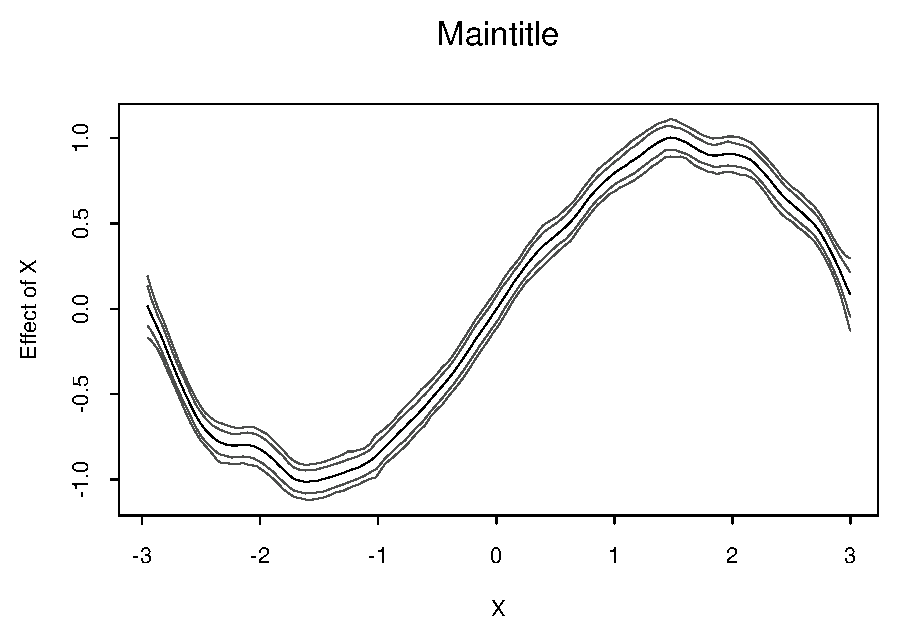
\includegraphics[scale=0.8]{grafiken/plotnonp.eps}
{\em\caption{ \label{illgraph} Illustration for the usage of
\em\tt plotnonp}}
\end{center}
\end{figure}

This statement draws the estimated effect of #X# and stores the
graph in the postscript file
#"c:#$\backslash$$\backslash$#bayes#$\backslash$$\backslash$#b_f_X_rw.ps"#.
A title, a x-axis and y-axis label is added to the graph. For
illustration purposes, the resulting graph is shown in
\autoref{illgraph}.

In some situations the effect of a covariate representing dates
must be plotted. Suppose for example that a covariate has values
ranging from 1 to 19 representing the time period from January
1983 to July 1984. In this case, we naturally prefer that the
x-axis is labelled in terms of dates rather than in the original
coding (from 1 to 19). To achieve this, function #plotnonp#
provides the three additional options #year#, #month# and #step#.
Options #year# and #month# are used to specify the year and the
month (1 for January, 2 for February, \dots) corresponding to the
minimum covariate value. In the example mentioned above
#year=1983# and #month=1# will produce the correct result. In
addition, option #step# may be specified to define the periodicity
in which your data are collected. For example #step=12# (the
default) corresponds to monthly data, while #step=4#, #step=2# and
#step=1# correspond to quarterly, half yearly and yearly data. We
illustrate the usage of #year#, #month# and #step# with our
example. Suppose we estimated the effect of calendar time #D#,
say, on a certain dependent variable, where the range of the data
is as described above. Then the following S-plus function call
will produce the postscript file shown in \autoref{illgraph2}:

\begin{figure}[ht]
\begin{center}
%\includegraphics[scale=0.8]{fvdate.eps}
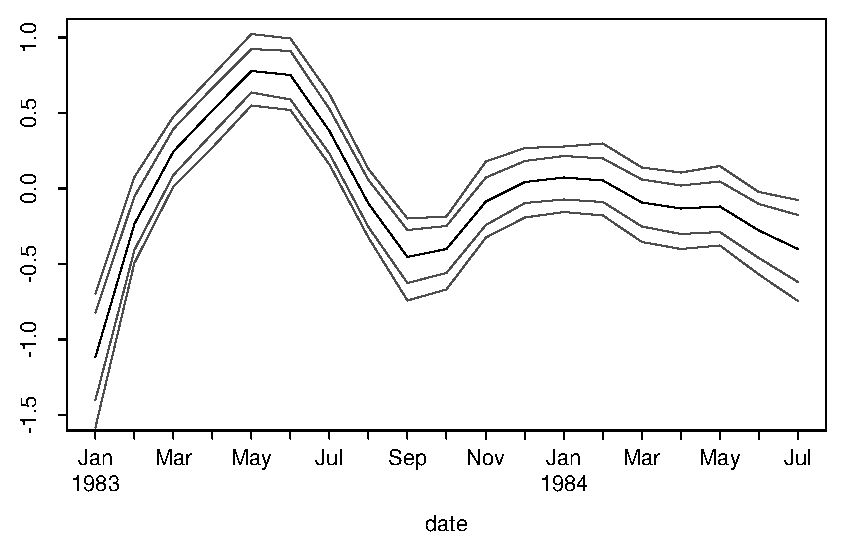
\includegraphics[scale=0.8]{grafiken/plotnonpdate.eps}
{\em\caption{ \label{illgraph2} Illustration for the usage of
\em\tt plotnonp}}
\end{center}
\end{figure}

#> plotnonp("c:\\bayes\\b_f_D_pspline.res", psname="c:\\bayes\\b_f_D_pspline.ps",#\\
#  year=1983,month=1,step=12,xlab="date", ylab= " ") #

Note, that \texttt{ylab=" "} forces S-plus to omit the y axis
label. If #ylab# (as well as #xlab#) is omitted, default labels
will be given to the two axis.

Finally, we note that all options that can be passed to the #plot#
function of S-plus may also be passed to function #plotnonp#.
Thus, function #plotnonp# is more or less a specialized version of
the S-plus #plot# function.


\subsubsection{Drawing geographical maps}
\index{S-plus!drawing geographical maps} \index{drawing
geographical maps}

This subsection describes how to visualize estimation results of
spatial covariates, where the observations represent the location
or site in connected geographical regions. A typical example for a
spatial covariate is given in the 'rents for flats' example, see
\autoref{rentdata}, where the covariate #L# indicates the location
(in subquarters) of the flat in Munich. \autoref{munich} shows a
map of Munich separated into subquarters.

\begin{figure}
\centering
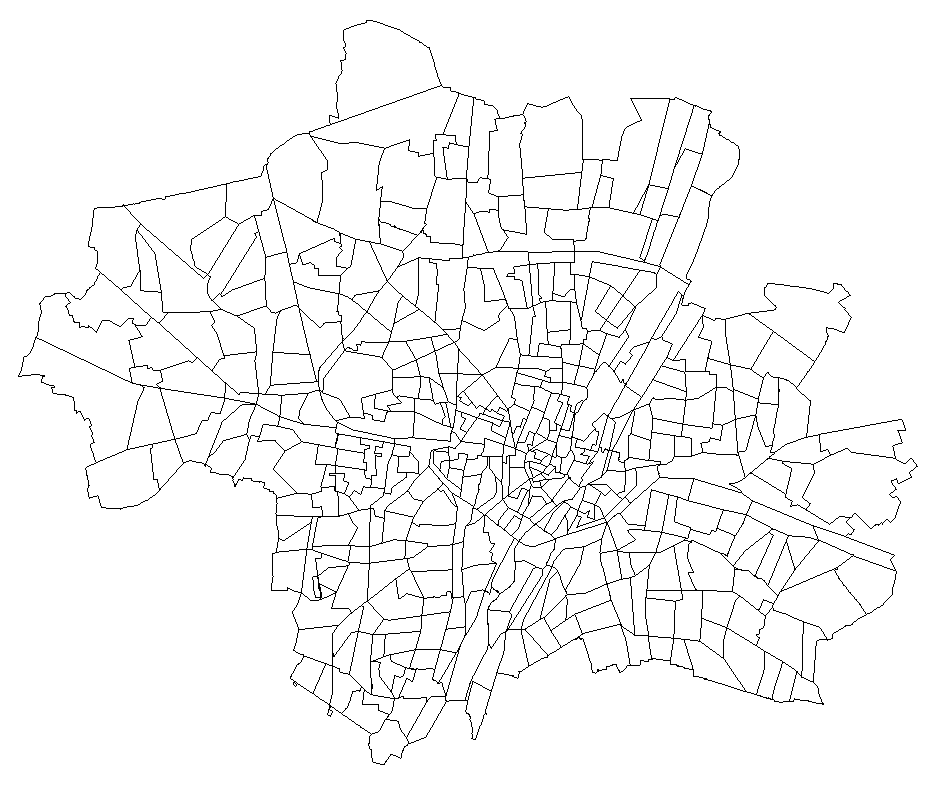
\includegraphics [scale=0.5]{grafiken/munich.eps}
{\em\caption{\label{munich} Map of Munich}}
\end{figure}


Typically, the effect of such a spatial covariate is incorporated
into a regression model via an unstructured or structured random
effect. In the latter case a spatial smoothness prior for the
spatial covariate is specified that penalizes too abrupt changes
of the estimated effect in neighboring sites. In some situations
the incorporation of both, an unstructured and a structured
effect, may also be appropriate. Details on how to incorporate
spatial covariates into a semiparametric regression  model are
given in \autoref{bayesregress}. For the rest of this section we
assume that an effect of a spatial covariate has already been
estimated and that we now want to visualize the estimation
results. This can be easily done with the two S-plus functions
#readbndfile# and #drawmap#. Function #readbndfile# is used to
read the boundary information of a map that is stored in a so
called boundary file and to store this information as a permanent
S-plus {\em map object}. The boundary file contains mainly the
polygons which form the different geographical regions of the map.
The required structure of such a file is described below. After
the successful reading of the boundary information of a map, the
second function #drawmap# may be used to draw and print the map
either on the screen or into a postscript file. There are several
possible ways to draw the map. In the simplest case the map can be
drawn without any estimation effects, i.e.~only the boundaries of
the different regions or sites are drawn, see \autoref{munich} for
an example. In practice, however, one usually wants to color the
regions of the map according to some numerical characteristics. As
an example compare \autoref{munichrelfreq} in which the
subquarters of Munich are colored according to the frequency of
flats in the 'rents for flats' data set located in the respective subquarter.
Subquarters colored in red contain less flats compared to
subquarters colored in green. In striped areas no observations are
available.

\begin{figure}[ht]
\begin{center}
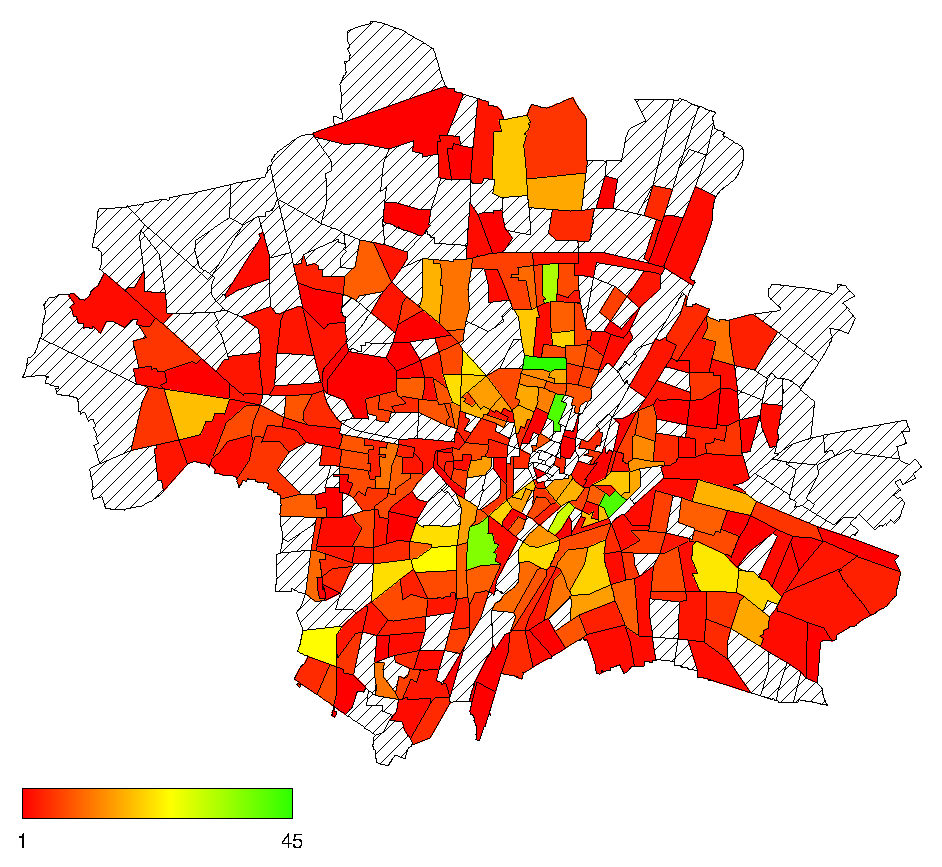
\includegraphics[scale=0.5]{grafiken/munichfr.eps}
{\em\caption{ \label{munichrelfreq} relative frequencies of
observed flats in the 'rents for flats' data set}}
\end{center}
\end{figure}


In the following we give a detailed description of the usage of
the functions #readbndfile# and #drawmap#.

{\bf Function readbndfile}
\medskip
\index{S-plus!reading boundary files} \index{reading boundary
files}

Function #readbndfile# is used to read in boundary information
stored in a boundary file into S-plus. The function has two
required arguments. The first argument is the filename of the
boundary file to read in. The second argument specifies the name
of the {\em map object} in S-plus (recall that the map information
is stored as a permanent S-plus object). To give an example,
suppose that {\em BayesX} is installed in the directory
#c:#$\backslash$#bayes# and that we want to read in the map of
Munich. In this case the boundary file of the map is stored in the
subdirectory #examples# of the installation directory, that is in
#c:#$\backslash$#bayes#$\backslash$#examples#. The name of the
boundary file is simply #munich.bnd#. The following function call
reads in the boundary information of Munich and stores the map
permanently in S-plus:

#> readbndfile("c:\\bayes\\examples\\munich.bnd","munich")#

Once again, note that double backslashes are required in S-plus to
specify a directory. The second argument in the statement above is
"munich", i.e.~the name of the map object is simply #munich#. To
refer to the map of Munich in subsequent statements and function
calls, the quotation marks must be omitted.

{\bf Function drawmap}
\medskip
\index{S-plus!drawmap}

Function #drawmap# is used to draw geographical maps and color the
regions according to some numerical characteristics. There is only
one required argument that must be passed to #drawmap#, that is
the name of the map to be drawn. Provided that the map has already
been read into S-plus (via function #readbndfile#), the following
statement draws the map of Munich in a S-plus graphic-window on
the screen:

#> drawmap(map=munich)#

Storing the map in a postscript file rather than drawing it on the
screen can be achieved by specifying the name of the postscript
file using the #outfile# option. For example the command

#> drawmap(map=munich,outfile="c:\\bayes\\munich.ps")#

produces a postscript file named #munich.ps# with the map of
Munich.

However, in most cases one not only wants to draw the boundaries
of a geographical map, but also color the regions according to
some numerical characteristics. Suppose for example that we have
already estimated a location specific effect on the monthly rents
in the 'rents for flats' data set. Suppose further that the
estimated effects are stored in
#c:#$\backslash$#bayes#$\backslash$#output#$\backslash$#b_f_L_spatial.res#.
The structure of the file is described in detail in
\autoref{bayesregress}. It contains 10 columns, one column with a
row counter, one column containing the values of the covariate
(here the location) and four columns containing estimated effects
for the values of the covariate. These are the posterior mean and
the posterior 2.5\%, 10\%, 50\%, 90\% and 97.5\% quantiles. The
last two columns contain posterior probabilities based on nominal
levels of 95\% and 80\%. The number 1 corresponds to a strictly
positive credible interval, the number -1 corresponds to a
strictly negative credible interval. A value of 0 indicates that
the corresponding credible interval contains zero. The first row
contains the column names. For the covariate #L# (location) for
example, the  first row of the file is given by:

 intnr   L  pmean   pqu2p5   pqu10   pmed   pqu90   pqu97p5 pcat95 pcat80

Suppose now that we want to visualize estimation results for the
spatial covariate #L# by coloring the subquarters of Munich
according to the estimated posterior mean. Compared to the S-plus
statement above, (at least) three more arguments must be passed to
function #drawmap#; the argument #dfile# that specifies the
filename of estimated results, the argument #plotvar# that
specifies the variable to be plotted and the argument #regionvar#
that specifies which column of the file, containing estimation
results, stores the region names. The following statement produces
the desired result:

 #> drawmap(map=munich,outfile="c:\\bayes\\munich.ps", #\\
 #  dfile="c:\\bayes\\output\\b_f_L_spatial.res", plotvar="pmean",regionvar="L")#


Note that the right hand side of options #plotvar# and #regionvar#
must be enclosed by quotation marks.

{\bf Optional arguments of function drawmap}

Besides the arguments discussed so far there are some more
optional arguments that can be passed to #drawmap#. They are
listed and described below together with a summary of the
arguments already described:


\begin{itemize}
\item {\bf map = characterstring}

Name of the S-plus {\em map object}. Use function #readbndfile# to
read in geographical maps into S-plus.
\item {\bf dfile = "filename (including path)"}

Filename (including path) of the file containing numerical
characteristics of the regions of the map. The file must contain
at least two columns, one column that lists the names of the
regions and one column containing the numerical characteristics of
the respective regions. It is important that the names of the
regions listed match with the region names stored in the S-plus
{\em map object}. The first row of the file must contain the names
of the columns.
\item {\bf outfile = "filename (including path)"}

Filename (including path) of the postscript file where the map
should be stored.
\item {\bf regionvar = "characterstring"}

Name of the column in the data file containing the region names
(see also argument #dfile#). Note that the right hand side must be
enclosed by quotation marks.
\item {\bf plotvar = "characterstring"}

Name of the column in the data file containing the numerical
characteristics of the regions (see also argument #dfile#). Note
that the right hand side must be enclosed by quotation marks.
\item {\bf lowerlimit = realvalue}

Lower limit of the range to be drawn. If #lowerlimit# is omitted,
the minimum numerical value in the #plotvar# column will be used
instead as the lower limit.
\item {\bf upperlimit = realvalue}

Upper limit of the range to be drawn. If #upperlimit# is omitted,
the maximum numerical value in the #plotvar# column will be used
instead as the upper limit.
\item {\bf nrcolors = integer}

To color the regions according to their numerical characteristics,
the data are divided into a (typically large) number of ordered
categories. Afterwards a color is associated with each category.
The #nrcolors# option can be used to specify the number of
categories (and with it the number of different colors). Default
value is 100.
\item {\bf pstitle = "characterstring"}

Adds a title to the graph. Note that the right hand side must be
enclosed by quotation marks.
\item {\bf color = T/F}

The #color# option allows to choose between a grey scale for the
colors and a colored scale. The default is #color=F#, which means
a grey scale.
\item {\bf legend = T/F}

By default a legend is drawn into the graph. To omit the legend in
the graph, #legend=F# must be passed as an additional argument.
\item {\bf drawnames = T/F}

In some situations it may be favorable to print the names of the
regions into the graph (although the result may be confusing in
most cases). This can be done by specifying the additional option
#drawnames=T#. By default the names of the regions are omitted in
the graph.
\item {\bf swapcolors = T/F}

In some situations it may be favorable to swap the order of the
colors, i.e.~red shades corresponding to large values and green
shades corresponding to small values. This is achieved by
specifying #swapcolors=T#. By default small values are colored in
red shades and large values in green shades.
\item {\bf pcat = T/F}

If you want to visualize the values of the columns #pcat80# or
#pcat95# it is convenient to specify #pcat=T#. This forces
#drawmap# to expect a column that consists only of the values -1,
0 and 1. Of course you can achieve the same result by setting
#nrcolors=3#, #lowerlimit=-1# and #upperlimit=1#. The default is
#pcat=F#.
\end{itemize}


\subsubsection{Plotting autocorrelation functions}
\label{splusplotautocor} \index{S-plus!plotting autocorrelation
functions} \index{plotting autocorrelation functions}
\index{autocorrelation functions!plotting}

This section describes how to visualize autocorrelation functions
of sampled parameters using the S-plus function #plotautocor#.

To compute autocorrelation functions, the post-estimation command
#autocor# must be applied, see \autoref{bayesautocorr} for
details. For the rest of this section we assume that
autocorrelations are already computed and stored in file:

#c:#$\backslash$#bayes#$\backslash$#output#$\backslash$#b_autocor.raw#

The minimum number of arguments required for the function is one,
namely the file where the computed autocorrelation functions are
stored. In this case a S-plus {\em graphic window} will be opened
and the autocorrelation functions are plotted on the screen. To
store autocorrelations in a postscript file, an output filename
must be specified as a second argument. Thus, the S-plus command

#> plotautocor("c:\\bayes\\output\\b_autocor.raw")#

prints autocorrelations on the screen, while the statement

 #> plotautocor("c:\\bayes\\output\\b_autocor.raw","c:\\bayes\\output\\b_autocor.ps")#

forces S-plus to store the autocorrelation graphs in the
postscript file #c:\bayes\output\b_autocor.ps#.

In particular for regression models with a large number of
parameters the execution of function #plotautocor# can be very
time consuming. Moreover, the size of the resulting postscript
file can be very large. To avoid such problems #plotautocor#
provides the additional argument #mean.autocor#. If
#mean.autocor=T# is specified, for each lag number and model term
only minimum, mean and maximum autocorrelations are plotted,
leading in most cases to a considerable reduction in computing
time and storing size.


\subsubsection{Plotting sampled parameters}
\label{splusplotsample} \index{S-plus!plotting sampled parameters}
\index{plotting sampled parameters}

This section describes how to plot sampled parameters using the
S-plus function #plotsample#. Before applying function
#plotsample#, sampled parameters must be stored in ASCII-format
using the post-estimation command #getsample#. See
\autoref{bayesgetsample} for details, but note that sampled
parameters will be stored in several different files, typically
one file for each term in the model.

Suppose now that we want to visualize sampling paths for the
parameters of the nonlinear effect of a covariate X. Assume
further that sampled parameters are stored in the ASCII file

#c:\bayes\output\b_X_sample.raw#.

As most other functions, #plotsample# provides two possibilities
of drawing sampled parameters. The first possibility is to print
the graphs on the screen, and the second is to store them into a
postscript file. To print the sampling paths on the screen, only
the filename (including path) of the ASCII file where sampled
parameters are stored must be passed to the function. For the
example mentioned above the corresponding command is:

#> plotsample("c:\\bayes\\output\\b_X_sample.raw")#

If sampling paths should be drawn into a postscript file rather
than on the screen, the filename of the resulting postscript file
must be specified as a second argument. Thus, for our example we
get:

 #> plotsample("c:\\bayes\\output\\b_X_sample.raw","c:\\bayes\\output\\b_X_sample.ps")#

In addition, all options that are available for the S-plus
function #plot# may be passed to function #plotsample#, see the
S-plus documentation for details.


\subsubsection{Plotting 2 dimensional surfaces}

This subsection describes the usage of the function #plotsurf# for
visualizing 2 dimensional surfaces. The function #plotsurf# merely
invokes different S-plus functions for visualizing 2 dimensional
data. Thus, users familiar with S-plus may prefer to use this
functions directly to gain more flexibility. Note that this function
is only available for S-plus.

Suppose that a Bayesian regression model has already been
estimated with predictor

$$
\eta = \dots + f(X1,X2) + \dots,
$$

where the interaction effect of #X1# and #X2# is modelled
nonparametrically using 2 dimensional P-splines and that the
estimation results are stored in file:

#c:\bayes\output\b_f_X1_X2_pspline.res#

The S-plus function #plotsurf# requires at least one argument,
which is the name (including path) of the file containing the
estimation results. For example the command

#> plotsurf("c:\\bayes\\output\\b_f_X1_X2_pspline.res")#

prints the posterior means against #X1# and #X2# on the screen.
There are several additional options that can be passed, for
example for changing the plot type or storing the graph as a
postscript file rather than displaying it on the screen. The
following list describes all possible arguments that may be passed
to the function #plotsurf#:

\begin{itemize}
\item {\bf data = "filename (including path)"}

Name (including path) of the file containing the estimation
results. The file must contain at least 3 columns, one for the
x-axis, one for the y-axis and one for the z-axis. The file must
contain a header.
\item {\bf outfile = "filename (including path)"}

Name (including path) of the postscript file where the graph
should be stored. This option is only meaningful for #mode=2# and
#mode=3#.
\item {\bf cols = 3 column vector}

This option is only meaningful, if the argument #data# is
specified. In this case #cols# gives the columns of the object or
data file passed to the argument #data#, that should be used as
values for the x, y and z axis. The default is #cols=c(2,3,4)#
which corresponds to plotting the posterior means against #X1# and
#X2#.
%\item {\bf zlim = 2 column vector}

%2 column vector giving the minimum and maximum value to be put on
%the z-axis.
\item {\bf mode = 1/2/3/4/5}

This option specifies the plot type. Currently there are 5
different types available. The default is #mode=1#, which
corresponds to what is called a 'Surface Plot' in S-plus.
\end{itemize}


\section{Global options}
\label{bayesregglobopt} \index{bayesreg object!global options}

The purpose of global options is to affect the global behavior of
a {\em bayesreg object}. The main characteristic of global options
is, that they are not associated with a certain method.

The syntax for specifying global options is

#> #{\em objectname}.{\em optionname} = {\em newvalue}

where {\em newvalue} is the new value of the option. The type of
the value depends on the respective option.

The following global options are currently available for {\em
bayesreg objects}:

\begin{itemize}
\item {\bf outfile = filename} \\
By default, the estimation output produced by the #regress#
procedure will be written to the default output directory, which
is

$<$#INSTALLDIRECTORY#$>$$\backslash$#output#.

The default filename is composed of the name of the {\em bayesreg
object} and the type of the file. For example, if you estimated a
nonparametric effect for a covariate #X#, say, then the estimation
output will be written to

$<$#INSTALLDIRECTORY#$>$$\backslash$#output#$\backslash$#b_nonpX.res#

where #b# is the name of the {\em bayesreg object}. In most cases,
however, it may be necessary to save estimation results into a
different directory and/or under a different filename than the
default. This can be done using the #outfile# option. With the
#outfile# option you have to specify the directory where the
output should be stored to and in addition a base filename. The
base filename should not be a complete filename. For example
specifying

#> b.outfile = c:\data\res#

would force {\em BayesX} to store the estimation result for the
nonparametric effect of #X# in file

#c:\data\res_nonpX.res#

\item {\bf iterationsprint = integer}

By default, the current iteration number is printed in the {\em
output window} (or in an additional log file) after every 100th
iteration. This can lead to rather big and complex output files.
The #iterationsprint# option allows to redefine after how many
iterations the current iteration number is printed. For example
#iterationsprint=1000# forces {\em BayesX} to print the current
iterations number only after every 1000th iteration rather than
after every 100th iteration.
\end{itemize}



\section{Examples}
\label{bayesregexamples}

In this Section we present a couple of complex examples about the
usage of {\em bayesreg objects}. The first example contains a
reanalysis of the 'credit scoring' data set that is described in
\autoref{creditdata}, which contains also a (incomplete) list of
some publications where the 'credit scoring' data set has already
been analyzed. The second example is a Bayesian analysis of
determinants of childhood undernutrition in Zambia. The data set
is described in \autoref{zambia}. This section contains also a
list of publications where the data set has been analyzed. Both
data sets are shipped together with {\em BayesX} and are stored in
the directory #examples#, which is a subdirectory of the
installation directory. Since the main focus here is on
illustrating the usage of {\em bayesreg objects}, we omit any
interpretation of estimated effects.


\subsection{Binary data: credit scoring}
\label{creditanalyse}

All {\em BayesX} statements of this section can be found in the
#examples# directory in the file #credit.prg#. In principle, the
commands in #credit.prg# can be executed using the #usefile#
command for running batch files, see \autoref{batch}. Note,
however, that the specified directories therein may not exist on
your computer. Thus, to avoid errors, the file must be modified
first to execute correctly.

\subsubsection{Reading the data into BayesX}


In order to analyze the 'credit scoring' data set, we first have
to load the data set into {\em BayesX}. For the rest of this
section we assume that {\em BayesX} is installed in the directory
#c:#$\backslash$#bayes#. In this case, the 'credit scoring' data
set can be found in #c:#$\backslash$#bayes#$\backslash$#examples#
under the name #credit.raw#. With the following two commands
(entered in the {\em command window}) we first create a {\em
dataset object} #credit# and afterwards load the data set into
{\em BayesX} using the #infile# command:

#> dataset credit# \\
#> credit.infile using c:\bayes\examples\credit.res#

Since the first row of the file already contains the variable
names, it is not necessary to specify variable names in the
#infile# statement. If the first row of the data set does not
contain the variable names, they must be additionally specified in
the #infile# command, e.g.~for the 'credit scoring' data set we
get

#> credit.infile y account duration amount payment intuse marstat# \\
#  using c:\bayes\examples\credit.res#


We now compute effect coded versions of the categorical covariates
#account#, #payment#, #intuse# and #marstat#:

#> credit.generate account1  = 1*(account=1)-1*(account=3)# \\
#> credit.generate account2  = 1*(account=2)-1*(account=3)# \\
#> credit.generate payment1 = 1*(payment=1)-1*(payment=2)# \\
#> credit.generate intuse1 = 1*(intuse=1)-1*(intuse=2)# \\
#> credit.generate marstat1 = 1*(marstat=1)-1*(marstat=2)#

The reference categories for the covariates are chosen to be 3 for
#account# and 2 for the others.

\subsubsection{Creating a bayesreg object}

Before we are able to estimate Bayesian regression models, we
first have to create a {\em bayesreg object}:

#> bayesreg b# \\
#> b.outfile = c:\results\credit#

The second command changes the default output directory and name
(which is #c:\bayes\output\b#) to
#c:\results\credit#. This means that
subsequent regression output is stored in the directory
#c:\results# and that all filenames start with
#credit#.

\subsubsection{Probit models}

\label{credit_probit} We can now start estimating models. We first
describe how probit models are estimated. The estimation of probit
models is slightly faster than logit models because the full
conditionals of the effects are Gaussian.

We first estimate a model with fixed effects only:

#> b.regress  y = account1 + account2 + duration + amount + payment1 + intuse1 #\\
#  + marstat1, predict iterations=6000 burnin=1000 step=5 family=binomialprobit # \\
#  using credit #

Here we specified 6000 iterations, a burnin period of 1000
iterations and a thinning parameter of 5, i.e.~every 5th sampled
parameter will be stored and used for estimation. The additional
option \hyperref[predict]{#predict#} is used to compute samples of
the deviance, the effective number of parameters, the deviance
information criteria (DIC), predicted means etc.

Executing the command yields the following output (simulation
output omitted):

\small

\begin{verbatim}

SIMULATION TERMINATED

SIMULATION RUN TIME: 13 seconds


ESTIMATION RESULTS:

  Predicted values:

  Estimated mean of predictors, expectation of response and
  individual deviances are stored in file
  c:\results\credit_predictmean.raw

  Estimation results for the Deviance:

  Unstandardized Deviance (-2*Loglikelihood(y|mu))

  Mean:             1027.05
  Std. Dev:         4.22501
  2.5% Quantile:    1021.01
  10% Quantile:     1022.48
  50% Quantile:     1026.29
  90% Quantile:     1032.73
  97.5% Quantile:   1037.28

  Saturated Deviance (-2*Loglikelihood(y|mu) + 2*Loglikelihood(y|mu=y))

  Mean:             1027.05
  Std. Dev:         4.22501
  2.5% Quantile:    1021.01
  10% Quantile:     1022.48
  50% Quantile:     1026.29
  90% Quantile:     1032.73
  97.5% Quantile:   1037.28

  Samples of the deviance are stored in file
  c:\results\credit_deviance_sample.raw

  Estimation results for the DIC:

  DIC based on the unstandardized Deviance

  Deviance(bar_mu):           1018.85
  pD:                         8.20049
  DIC:                        1035.26

  DIC based on the saturated Deviance

  Deviance(bar_mu):           1018.85
  pD:                         8.20049
  DIC:                        1035.26




  FixedEffects1


  Acceptance rate:    100 %


  Variable  mean           Std. Dev.      2.5% quant.    median         97.5% quant.
  const     -0.715437      0.117673       -0.9464        -0.710836      -0.49298
  account1  -0.629553      0.0684571      -0.764526      -0.6244        -0.50343
  account2  0.50699        0.0625032      0.389608       0.506698       0.63888
  duration  0.0204795      0.00471734     0.0111948      0.0205776      0.0298505
  amount    0.0172111      0.0189096      -0.0173778     0.0167277      0.0542619
  payment1  -0.2919        0.0762402      -0.438703      -0.288309      -0.152512
  intuse1   -0.137287      0.0477423      -0.228492      -0.137755      -0.041511
  marstat1  -0.158195      0.0476991      -0.254198      -0.157534      -0.0663364

  Results for fixed effects are also stored in file
  c:\results\credit_FixedEffects1.res
\end{verbatim}


\normalsize

Somewhat surprisingly, we observe that the amount of credit seems
to have no ('significant') influence on the response. To check
this phenomenon more carefully, we run a second estimation, now
allowing for possibly nonlinear effects of the continuous
covariates #amount# and #duration#. We choose cubic P-splines with
second order random walk penalty as smoothness priors and modify
the #regress# statement above according to the new model:

#> b.regress  y = account1 + account2 + duration(psplinerw2) + amount(psplinerw2)# \\
#  + payment1 + intuse1 + marstat1, predict iterations=6000 burnin=1000 step=5# \\
#  family=binomialprobit using credit #

We get the following output for the nonlinear functions (output
for the rest omitted):

\small

\begin{verbatim}

  f_duration_pspline


  Acceptance rate:    100 %

  Results are stored in file c:\results\credit_f_duration_pspline.res

  Postscript file is stored in file c:\results\credit_f_duration_pspline.ps

  Results may be visualized using method 'plotnonp'
  Type for example: objectname.plotnonp 1


  f_duration_pspline_variance


  Acceptance rate:    100 %

  Estimation results for the variance component:

  Mean:             0.00787338
  Std. dev.:        0.0100301
  2.5% Quantile:    0.00128376
  10% Quantile:     0.00190016
  50% Quantile:     0.00487717
  90% Quantile:     0.0157856
  97.5% Quantile:   0.0315107

  Results for the variance component are also stored in file
  c:\results\credit_f_duration_pspline_var.res


  f_amount_pspline


  Acceptance rate:    100 %

  Results are stored in file c:\results\credit_f_amount_pspline.res

  Postscript file is stored in file c:\results\credit_f_amount_pspline.ps

  Results may be visualized using method 'plotnonp'
  Type for example: objectname.plotnonp 3


  f_amount_pspline_variance


  Acceptance rate:    100 %

  Estimation results for the variance component:

  Mean:             0.00870842
  Std. dev.:        0.0115895
  2.5% Quantile:    0.0013844
  10% Quantile:     0.00220351
  50% Quantile:     0.00570725
  90% Quantile:     0.0164858
  97.5% Quantile:   0.0340326

  Results for the variance component are also stored in file
  c:\results\credit_f_amount_pspline_var.res
\end{verbatim}


\normalsize


We  visualize estimated effects for #amount# and #duration# using
method #plotnonp# (as advised by the program):

#> b.plotnonp 1 , outfile="c:\results\credit_duration.ps"#\\
#> b.plotnonp 3 , outfile="c:\results\credit_amount.ps"#

This produces the graphs (stored in postscript files) shown in
\autoref{creditfigures}.

\begin{figure}[ht]
\vspace{0.5cm}
\begin{center}
\includegraphics[scale=0.65]{grafiken/credit_duration.ps}

\vspace{0.5cm}
\includegraphics[scale=0.65]{grafiken/credit_amount.ps}
\end{center}
{\em\caption{ \label{creditfigures} Estimated effects of duration
and amount of credit. Shown is the posterior mean within 80\% and
95\% credible regions.}}
\end{figure}

We add a title, x-axis and y-axis labels by typing \hfill

#> b.plotnonp 1 , outfile="c:\results\credit_duration.ps" replace #\\
#  xlab="duration" ylab="f(duration)" title="effect of duration"#

#> b.plotnonp 3 , outfile="c:\results\credit_amount.ps" replace# \\
#  xlab="amount" ylab="f(amount)" title="effect of amount"#

and obtain the improved graphs shown in \autoref{creditfigures_2}.
The option #replace# is specified to allow {\em BayesX} to
overwrite the previously generated postscript files. If the
#outfile# option is omitted, the graphs are printed on the screen
rather than being stored as postscript files.

\begin{figure}[ht]
\vspace{0.5cm}
\begin{center}
\includegraphics[scale=0.65]{grafiken/credit_duration_2.ps}

\vspace{0.5cm}
\includegraphics[scale=0.65]{grafiken/credit_amount_2.ps}
\end{center}
{\em\caption{ \label{creditfigures_2} Improved plots of the effect
of {\em\tt duration} and {\em\tt amount}.}}
\end{figure}


We now want to check the mixing of the generated Markov chains,
although the mixing for probit models is usually excellent. For
that reason we compute and plot the autocorrelation functions by
typing:

#> b.plotautocor , outfile="c:\results\credit_autocor.ps"#

We obtain the file
#c:#$\backslash$#results#$\backslash$#credit_autocor.ps# containing 9
pages of autocorrelation functions for all parameters in the
model. The first page of this file is shown in
\autoref{credit_autocor1}. We see that autocorrelations die off
very quickly.

\begin{figure}[ht]
\vspace{0.5cm}
\begin{center}
\includegraphics[scale=0.8]{grafiken/credit_autocor1.ps}
\end{center}
{\em\caption{ \label{credit_autocor1} First page of the
autocorrelation file.}}
\end{figure}

\clearpage

\subsubsection{Logit models}

A logit model rather than a probit model is estimated by replacing
#family=binomialprobit# with #family=binomial#:

#> b.regress  y = account1 + account2 + duration(psplinerw2) + amount(psplinerw2)# \\
#  + payment1 + intuse1 + marstat1, predict iterations=6000 burnin=1000 step=5# \\
#  family=binomial using credit#

In contrast to binary probit models, the full conditionals for the
regression coefficients are no longer Gaussian. {\em BayesX}
offers 3 different types of proposal densities. These are
iteratively weighted least squares (IWLS) proposals based either
on the current state of the parameters or on the posterior modes
as described in \autoref{IWLS} or Brezger and Lang (2003), and
conditional prior proposals as described in Fahrmeir and Lang
(2001b). We recommend the usage of IWLS proposals, since no tuning
is required and mixing properties are superior to those of
conditional prior proposals. The default are IWLS proposals based
on the current state of the parameters. The following statement
causes {\em BayesX} to use IWLS proposals based on posterior
modes, which usually yield even higher acceptance probabilities
compared to ordinary IWLS proposals:

#> b.regress  y = account1 + account2 + duration(psplinerw2,proposal=iwlsmode)# \\
#  + amount(psplinerw2,proposal=iwlsmode) + payment1 + intuse1 + marstat1,# \\
#  predict iterations=6000 burnin=1000 step=5# \\
#  family=binomial using credit#

As for the probit model, we visualize the estimated nonlinear
effects of #duration# and #amount# using method #plotnonp#:

#> b.plotnonp 1 , outfile="c:\results\credit_logit_duration.ps" replace# \\
#  xlab="duration" ylab="f(duration)" title="effect of duration" #

#> b.plotnonp 3 , outfile="c:\results\credit_logit_amount.ps" replace# \\
#  xlab="amount" ylab="f(amount)" title="effect of amount" #

The resulting graphs are shown in \autoref{creditlogit}. As could
have been expected only the scale of the estimated effects differs
(because of the logit link).

\begin{figure}[ht]
\vspace{0.5cm}
\begin{center}
\includegraphics[scale=0.65]{grafiken/credit_logit_duration.ps}

\vspace{0.5cm}
\includegraphics[scale=0.65]{grafiken/credit_logit_amount.ps}
\end{center}
{\em\caption{ \label{creditlogit} Effect of {\em\tt duration} and
{\em\tt amount}, if a logit model is estimated rather than a
probit model.}}
\end{figure}

Once again, to check the mixing of the sampled parameters we
compute and plot the autocorrelation functions using method
#plotautocor#:

#> b.plotautocor , outfile="c:\results\credit_logit_autocor.ps"#

The first page of the resulting postscript file is shown in
\autoref{creditautocorlogit_1}. As can be seen, the
autocorrelations for the logit model with IWLS proposals are
almost as low as for the probit model.

\begin{figure}[ht]
\vspace{0.5cm}
\begin{center}
\includegraphics[scale=0.8]{grafiken/credit_logit_autocor1.ps}
\end{center}
{\em\caption{ \label{creditautocorlogit_1} First page of the
autocorrelation file, if a logit model is estimated.}}
\end{figure}

\clearpage

\subsubsection{Varying the hyperparameters}

In the preceding examples we used the default hyperparameters
#a=0.001# and #b=0.001# for the inverse gamma prior of the
variances. In some situations, however, the estimated nonlinear
functions may considerably depend on the particular choice of
hyperparameters #a# and #b#. This may be the case for very low
signal to noise ratios or/and small sample sizes. It is therefore
highly recommended to estimate all models under consideration
using a (small) number of {\em different} choices for #a# and #b#
(e.g.~#a=1#,#b=0.005#; #a=0.001#,#b=0.001#; #a=0.0001#,#b=0.0001#)
to assess the dependence of results on minor changes in the model
assumptions. In that sense, the variation of hyperparameters can
be used as a tool for model diagnostics.

We estimate our probit model from \autoref{credit_probit} again,
but now with hyperparameters #a=1.0#, #b=0.005# and #a=0.0001#,
#b=0.0001#, respectively.

 #> b.regress  y = account1 + account2 + duration(psplinerw2,a=1.0,b=0.005) +# \\
 #  amount(psplinerw2,a=1.0,b=0.005) + payment1 + intuse1 + marstat1,# \\
 #  predict iterations=6000 burnin=1000 step=5 family=binomialprobit using credit #

 #> b.regress  y = account1 + account2 + duration(psplinerw2,a=0.0001,b=0.0001) +# \\
 #  amount(psplinerw2,a=0.0001,b=0.0001) + payment1 + intuse1 + marstat1, #\\
 #  predict iterations=6000 burnin=1000 step=5 family=binomialprobit using credit#

\autoref{credit_varhyper} shows the estimated nonlinear effects of
variables #duration# and #amount# with the different choices for
#a# and #b#. We see that in this example estimation results differ
only slightly for the different choices of #a# and #b#.


\begin{figure}[ht]
\vspace{0.5cm}
\begin{center}
\includegraphics[scale=0.4]{grafiken/credit_duration_a001b001.ps} \hspace{0.3cm}
\includegraphics[scale=0.4]{grafiken/credit_amount_a001b001.ps}

\vspace{0.5cm}
\includegraphics[scale=0.4]{grafiken/credit_duration_a1b005.ps} \hspace{0.3cm}
\includegraphics[scale=0.4]{grafiken/credit_amount_a1b005.ps}

\vspace{0.5cm}
\includegraphics[scale=0.4]{grafiken/credit_duration_a0001b0001.ps} \hspace{0.3cm}
\includegraphics[scale=0.4]{grafiken/credit_amount_a0001b0001.ps}
\end{center}
{\em\caption{ \label{credit_varhyper} Results for the effect of
{\em\tt duration} and {\em\tt amount} for different values of the
hyperparameters for the variances.}}
\end{figure}


\clearpage

\subsection{Determinants of childhood undernutrition in Zambia}

\label{zambiaanalysis} In this subsection we present a tutorial
like example for the usage of {\em bayesreg objects}. We use data
on undernutrition of children in Zambia, compare \autoref{zambia}
for a description of the data set. The files containing the data
and the map can be found in the subdirectory #examples# of the
installation directory together with the batch file
#mcmctutorial.prg# containing all commands used in the following
subsections.

The rest of the example is separated in seven parts dealing with
the different steps of estimating a regression model. In
\autoref{zambia_mcmc_datasets} we create a {\em dataset object} to
incorporate, handle and manipulate the data. We will also give a
brief description of some methods that may be applied to {\em
dataset objects}. Since we want to estimate a spatial effect of
the district in which a child lives, we need the boundaries of the
districts to compute the neighborhood information of the map of
Zambia. This information will be stored in a {\em map object}.
\autoref{zambia_mcmc_maps} describes how to create and handle
these objects. Estimation of the regression model is carried out
in \autoref{zambia_mcmc_regression} using a {\em bayesreg object}.
The next two sections describe how to visualize the estimation
results and how to customize the obtained graphics.
\autoref{zambia_mcmc_postest} describes post estimation commands
which can be used to investigate the sampling paths and the
autocorrelation functions of the estimated parameters. In a last
section we perform a sensitivity analysis to assess the impact of
hyperparameter choices on our estimation results.

Please note, that all paths within the following subsections must
be changed according to the storage location of the corresponding
files on your hard disk.

\subsubsection{Reading data set
information}\label{zambia_mcmc_datasets}

In a first step we read the available data set information into
{\it BayesX}. Therefore we create a {\it dataset object} named
#d#:

#> dataset d#

We store the data in #d# using the method #infile#:

#> d.infile, maxobs=5000 using c:\data\zambia.raw#

Note, that we assume the data to be provided in the external file
#c:\data\zambia.raw#. The first few lines of this file look like
this:

{\footnotesize
 hazstd bmi agc district rcw edu1 edu2 tpr sex\\
 0.0791769 \,\, 21.83 \,\, 4 \,\, 81 \,\, -1 \,\, 1 \,\, 0 \,\, 1 \,\, -1\\
 -0.2541965 \,\, 21.83 \,\, 26 \,\, 81 \,\, -1 \,\, 1 \,\, 0 \,\, 1 \,\, -1\\
 -0.1599823 \,\, 20.43 \,\, 56 \,\, 81 \,\, 1 \,\, -1 \,\, -1 \,\, 1 \,\, 1\\
 0.1733911 \,\, 22.27 \,\, 6 \,\, 81 \,\, -1 \,\, 0 \,\, 1 \,\, 1 \,\, 1}

In our example the file contains the variable names in the first
line. Therefore it is not necessary to specify them in the
#infile# command. If the file contained only the data without
variable names, we would have to supply them after the keyword
#infile#:

 #> d.infile hazstd bmi agc district rcw edu1 edu2 tpr sex, maxobs=5000#
 #  using c:\data\zambia.raw#


Option #maxobs# can be used to speed up the execution time of the
#infile# command. If #maxobs# is specified, {\it BayesX} allocates
enough memory to store all the data while the total amount of
required memory is unknown in advance if #maxobs# remains
unspecified. For larger data sets this may cause {\it BayesX} to
start reading the data set information several times because the
currently allocated memory is exceeded. However, this is only
meaningful for larger data sets with more than 10000 observations
and could therefore be omitted in our example.

A second option that may be added to the #infile# command is the
#missing# option to indicate missing values. Specifying for
example {\tt missing=M} defines the letter '{\tt M}' as an
indicator for a missing value. The default for missing values are
a period '.' and '{\tt NA}' (which remain valid indicators for
missing values even if an additional indicator is defined by the
{\tt missing} option).

After having read in the data set information we can inspect the
data visually. Executing the command

#> d.describe#

opens an {\it object-viewer window} containing the data in form of
a spreadsheet. This can also be achieved by double-clicking on the
{\it dataset object} in the {\it object browser}.

Further methods allow to examine the variables in the {\it dataset
object}. For a categorial variable, e.g.~#sex#, the #tabulate#
command may be used to produce a frequency table:

#> d.tabulate sex#

resulting in

\begin{verbatim}
Variable: sex

          Value       Obs           Freq            Cum
             -1      2451         0.5057         0.5057
              1      2396         0.4943              1
\end{verbatim}

being printed in the {\it output window}. For continuous variables
the #descriptive# command prints several characteristics of the
variable in the {\em output window}. E.g., executing

#> d.descriptive bmi#

leads to

\begin{verbatim}
   Variable    Obs        Mean      Median         Std         Min         Max
        bmi   4847   21.944349        21.4   3.2879659        12.8       39.29
\end{verbatim}

\subsubsection{Map objects}\label{zambia_mcmc_maps}

In the following we want to estimate a spatially correlated effect
of the district in which a child lives. Therefore we need the
boundaries of the districts in Zambia to compute the neighborhood
information of the map of Zambia. We therefore create a {\it map
object}

#> map m#

and read in the boundaries using the #infile# command of {\it map
objects}:

#> m.infile using c:\data\zambia.bnd#

Having read in the boundary information, {\it BayesX}
automatically computes the neighborhood matrix of the map.

The file following the keyword #using# is assumed to contain the
boundaries in form of closed polygons. Compare \autoref{map} for a
description of the expected file format.

{\it Map objects} may be visualized using method #describe#:

#> m.describe#

resulting in the graph shown in \autoref{zambia_mcmc_zambiamap}.
Additionally, #describe# prints further information about the {\it
map object} in the {\it output window} including the name of the
object, the number of regions, the minimum and maximum number of
neighbors and the bandwidth of the corresponding adjacency or
neighborhood matrix:

\begin{verbatim}
  MAP m
  Number of regions: 54
  Minimum number of neighbors: 1
  Maximum number of neighbors: 9
  Bandsize of corresponding adjacency matrix: 24
\end{verbatim}

\begin{figure}[ht]
\begin{center}
\epsfig{file=grafiken/zambia.ps,scale=0.35} {\it\caption{The
districts within Zambia.\label{zambia_mcmc_zambiamap}}}
\end{center}
\end{figure}


The numerical complexity associated with the estimation of
structured spatial effects using MCMC techniques depends
essentially on the structure of the neighborhood matrix. Often the
geographical information stored in a boundary file does not
represent the 'ideal' ordering (as regards to the estimation
problem) of the districts or regions. Therefore it may be useful
to reorder the map using method #reorder#:

#> m.reorder#

Usually reordering results in a smaller bandwidth although the
bandwidth is not the criterion that is minimized by #reorder#.
Instead the {\it envelope} of the neighborhood matrix is minimized
(compare George and Liu 1981).

In order to avoid reordering the {\it map object} every time you
start {\it BayesX} it is useful to store the reordered version in
a separate file. This can be achieved using the #outfile# command
of {\it map objects}:

#> m.outfile, replace using c:\data\zambiasort.bnd#

The reordered map is now stored in the given file. Note, that
specifying the option #replace# allows {\it BayesX} to overwrite
an existing file with the same name. Without this option an error
message would be raised if the given file is already existing.

Reading the boundary information from an external file and
computing the neighborhood matrix may be a computationally
intensive task if the map contains a large number of regions or if
the polygons are given in great detail. To avoid doing these
computation in every $BayesX$ session, we store the neighborhood
information in a so-called {\it graph file} using method #outfile#
together with the #graph# option (compare \autoref{map} for a
description of {\em graph files}):

#> m.outfile, replace graph using c:\data\zambiasort.gra#

To see how storing maps in {\it graph files} affects the
computation time of the #infile# command, we create a second {\it
map object} and read in the information from the graph file.
Again, we have to specify the keyword #graph#:

#> map m1#\\
#> m1.infile, graph using c:\data\zambiasort.gra#

As you should have noticed, reading geographical information from
a {\it graph file} is usually much faster than reading from a {\it
boundary file}. However, using {\it graph files} also has a
drawback. Since they do no longer contain the full information on
the polygons forming the map, we can not visualize a {\it map
object} created from a {\it graph file}. Trying to do so

#> m1.describe#

raises an error message. This implies, that visualizing estimation
results of spatial effects can only be based on {\it map objects}
created from {\it boundary files}, although estimation can be
carried out using {\it graph files}. Since we will work with the
{\it map object} #m# in the following, we delete #m1#:

#> drop m1#

\subsubsection{Bayesian semiparametric
regression}\label{zambia_mcmc_regression}

To estimate a regression model using MCMC techniques we first
create a {\it bayesreg object}:

#> bayesreg b#

By default estimation results are written to the subdirectory
#output# of the installation directory. In this case the default
filenames are composed of the name of the {\it bayesreg object}
and the type of the specific file. Usually it is more convenient
to store the results in a user-specified directory. To define this
directory we use the #outfile# command of {\it bayesreg objects}:

#> b.outfile = c:\data\b#

Note, that #outfile# does not only specify a directory but also a
base filename (the character #b# in our example). Therefore
executing the command above leads to storage of the results in the
directory #c:\data# and all filenames start with the character
#b#. Of course the base filename may be different from the name of
the {\it bayesreg object}.

In addition to parameter estimates {\it BayesX} also gives
acceptance rates for the different effects and some further
information on the estimation process. In contrast to parameter
estimates this information is not stored automatically but is
printed in the {\it output window}. Therefore it is useful to
store the contents of the {\it output window}. This can be
achieved automatically by opening a log file using the #logopen#
command

#> logopen, replace using c:\data\logmcmc.txt#

After opening a log file, every information written to the {\em
output window} is also stored in the log file. Option #replace#
allows {\it BayesX} to overwrite an existing file with the same
name as the specified log file. Without #replace# results are
appended to an existing file.

The model presented in Kandala et al.~(2001) is given by the
following semiparametric predictor:
\[\eta=\gamma_0+\gamma_1rcw+\gamma_2edu1+\gamma_3edu2+\gamma_4tpr+\gamma_5sex+f_1(bmi)+f_2(agc)+f^{str}(district)+f^{unstr}(district)\]
The two continuous covariates #bmi# and #agc# are assumed to have
a possibly nonlinear effect on the Z-score and are therefore
modelled nonparametrically (as P-splines with second order random
walk prior in our example). The spatial effect of the district is
split up into a spatially correlated part $ f^{str}(district)$ and
an uncorrelated part $f^{unstr}(district)$, see Fahrmeir and Lang
(2001b) for a motivation. The correlated part is modelled by a
Markov random field prior, where the neighborhood matrix and
possible weights associated with the neighbors are obtained from
the {\it map object} #m#. The uncorrelated part is modelled by an
i.i.d.~Gaussian effect.

To estimate the model we use method #regress# of {\em bayesreg
objects}:

 #> b.regress hazstd = rcw + edu1 + edu2 + tpr + sex + bmi(psplinerw2)#\\
 #  + agc(psplinerw2) + district(spatial,map=m) + district(random),#\\
 #  family=gaussian iterations=12000 burnin=2000 step=10 predict using d#

Options {\tt iterations}, {\tt burnin} and {\tt step} define
properties of the MCMC-algorithm. The total number of MCMC
iterations is given by {\tt iterations} while the number of burn
in iterations is given by {\tt burnin}. Therefore we obtain a
sample of 10000 random numbers with the above specifications.
Since, in general, these random numbers are correlated, we do not
use all of them but thin out the Markov chain by the thinning
parameter {\tt step}. Specifying {\tt step=10} as above forces
{\em BayesX} to store only every 10th sampled parameter which
leads to a random sample of length 1000 for every parameter in our
example.

Note, that the choice of {\tt iterations} also affects computation
time. On a 2.4 GHz PC estimation of our model took about 1 minute
and 5 seconds, which is rather fast in regard of the complexity of
the model.

If option {\tt predict} is specified, samples of the deviance, the
effective number of parameters $p_D$, and the deviance information
criteria $DIC$ of the model are computed, see Spiegelhalter et
al.~(2002). In addition, estimates for the linear predictor and
the expectation of every observation are obtained.

In the following we reproduce the content of the {\em output
window} to make the user familiar with the estimation results
produced by {\em BayesX}:

\footnotesize
\begin{verbatim}
ESTIMATION RESULTS:

  Predicted values:

  Estimated mean of predictors, expectation of response and
  individual deviances are stored in file
  c:\data\b_predictmean.raw

  Estimation results for the deviance:

  Unstandardized Deviance (-2*Loglikelihood(y|mu))

  Mean:             12688.959
  Std. Dev:         12.615837
  2.5% Quantile:    12663.847
  10% Quantile:     12673.03
  50% Quantile:     12688.804
  90% Quantile:     12705.921
  97.5% Quantile:   12714.078

  Saturated Deviance (-2*Loglikelihood(y|mu) + 2*Loglikelihood(y|mu=y))

  Mean:             4848.1335
  Std. Dev:         98.563486
  2.5% Quantile:    4657.7394
  10% Quantile:     4719.1869
  50% Quantile:     4847.534
  90% Quantile:     4971.7679
  97.5% Quantile:   5059.5874

  Samples of the deviance are stored in file
  c:\data\b_deviance_sample.raw

  Estimation results for the DIC:

  DIC based on the unstandardized deviance

  Deviance(bar_mu):           12639.654
  pD:                         49.305405
  DIC:                        12738.265


  DIC based on the saturated deviance

  Deviance(bar_mu):           4797.8139
  pD:                         50.31962
  DIC:                        4898.4532

  Estimation results for the scale parameter:

  Acceptance rate:   100 %

  Mean:             0.802517
  Std. dev.:        0.0164098
  2.5% Quantile:    0.768981
  10% Quantile:     0.782025
  50% Quantile:     0.802168
  90% Quantile:     0.824066
  97.5% Quantile:   0.83595


  FixedEffects1

  Acceptance rate:    100 %

  Variable  mean           Std. Dev.      2.5% quant.    median         97.5% quant.
  const     0.102975       0.0493194      0.00460694     0.102048       0.201918
  rcw       0.00782474     0.0129786      -0.0177587     0.0079339      0.0325389
  edu1      -0.0612525     0.0268997      -0.11368       -0.0622293     -0.00870588
  edu2      0.234627       0.0468064      0.146532       0.23578        0.322222
  tpr       0.0891162      0.0218746      0.0476786      0.0893937      0.133562
  sex       -0.058801      0.0130027      -0.083714      -0.0593365     -0.031744

  Results for fixed effects are also stored in file
  c:\data\b_FixedEffects1.res


  f_bmi_pspline

  Acceptance rate:    100 %

  Results are stored in file
  c:\data\b_f_bmi_pspline.res

  Postscript file is stored in file
  c:\data\b_f_bmi_pspline.ps

  Results may be visualized using method 'plotnonp'
  Type for example: objectname.plotnonp 1


  f_bmi_pspline_variance

  Acceptance rate:    100 %

  Estimation results for the variance component:

  Mean:             0.00192786
  Std. dev.:        0.00268103
  2.5% Quantile:    0.000281651
  10% Quantile:     0.000452872
  50% Quantile:     0.00119819
  90% Quantile:     0.00380296
  97.5% Quantile:   0.00806144

  Results for the variance component are also stored in file
  c:\data\b_f_bmi_pspline_var.res


  f_agc_pspline

  Acceptance rate:    100 %

  Results are stored in file
  c:\data\b_f_agc_pspline.res

  Postscript file is stored in file
  c:\data\b_f_agc_pspline.ps

  Results may be visualized using method 'plotnonp'
  Type for example: objectname.plotnonp 3


  f_agc_pspline_variance

  Acceptance rate:    100 %

  Estimation results for the variance component:

  Mean:             0.00600587
  Std. dev.:        0.00993897
  2.5% Quantile:    0.00119369
  10% Quantile:     0.00169024
  50% Quantile:     0.00397818
  90% Quantile:     0.0107538
  97.5% Quantile:   0.0227737

  Results for the variance component are also stored in file
  c:\data\b_f_agc_pspline_var.res


  f_district_spatial

  Acceptance rate:    100 %

  Results are stored in file
  c:\data\b_f_district_spatial.res

  Postscript file is stored in file
  c:\data\b_f_district_spatial.ps

  Results may be visualized in BayesX using method 'drawmap'
  Type for example: objectname.drawmap 5


  f_district_spatial_variance

  Acceptance rate:    100 %

  Estimation results for the variance component:

  Mean:             0.0359038
  Std. dev.:        0.0176849
  2.5% Quantile:    0.0117425
  10% Quantile:     0.0168868
  50% Quantile:     0.0321435
  90% Quantile:     0.0593765
  97.5% Quantile:   0.0807406

  Results for the variance component are also stored in file
  c:\data\b_f_district_spatial_var.res


  f_district_random

  Acceptance rate:    100 %

  Results for random effects are stored in file
  c:\data\b_f_district_random.res

  Results for the sum of the structured and unstructured
  spatial effects are stored in file
  c:\data\b_district_spatialtotal.res


  f_district_random_variance

  Acceptance rate:    100 %

  Estimation results for the variance component:

  Mean:             0.0077143
  Std. dev.:        0.00580379
  2.5% Quantile:    0.000703806
  10% Quantile:     0.00152536
  50% Quantile:     0.00648848
  90% Quantile:     0.0153428
  97.5% Quantile:   0.0215434

  Results for the variance component are also stored in file
  c:\data\b_f_district_random_var.res

  Files of model summary:

  ---------------------------------------------------------------------------

  Batch file for visualizing effects of nonlinear functions is stored in file
  c:\data\b_graphics.prg

  NOTE: 'input filename' must be substituted by the filename of the boundary-file

  ---------------------------------------------------------------------------

  Batch file for visualizing effects of nonlinear functions
  in S-Plus is stored in file
  c:\data\b_splus.txt

  NOTE: 'input filename' must be substituted by the filename of the boundary-file

  ---------------------------------------------------------------------------

  Latex file of model summaries is stored in file
  c:\data\b_model_summary.tex

  ---------------------------------------------------------------------------
\end{verbatim}
\normalsize

In addition to the information being printed to the {\em output
window} results for each effect are written to external ASCII
files. The names of these files are given in the {\em output
window}, compare the previous pages. The files contain the
posterior mean and median, the posterior 2.5\%, 10\%, 90\% and
97.5\% quantiles, and the corresponding 95\% and 80\% posterior
probabilities of the estimated effects. For example, the beginning
of the file #c:\data\b_f_bmi_pspline.res# for the effect of # bmi#
looks like this:

{\footnotesize
 intnr \,\, bmi \,\, pmean \,\, pqu2p5 \,\, pqu10 \,\, pmed \,\, pqu90 \,\, pqu97p5 \,\, pcat95 \,\, pcat80\\
 1 \,\, 12.8 \,\, -0.284065 \,\, -0.660801 \,\, -0.51678 \,\, -0.283909 \,\, -0.0585753 \,\, 0.085998 \,\, 0 \,\, -1\\
 2 \,\, 13.15 \,\, -0.276772 \,\, -0.609989 \,\, -0.483848 \,\, -0.275156 \,\, -0.070517 \,\, 0.0572406 \,\, 0 \,\, -1\\
 3 \,\, 14.01 \,\, -0.258674 \,\, -0.515628 \,\, -0.416837 \,\, -0.257793 \,\, -0.10009 \,\, -0.00289024 \,\, -1 \,\, -1}

The posterior quantiles and posterior probabilities may be changed
by the user using the options #level1# and #level2#. For example
specifying #level1=99# and #level2=70# in the options list of the
#regress# command leads to the computation of 0.5\%, 15\%, 85\%
and 99.5\% quantiles of the posterior. The defaults are
#level1=95# and #level2=80#.

Some nonparametric effects are visualized by {\em BayesX}
automatically and the resulting graphs are stored in ps format.
E.g.~the effect of #bmi# is visualized in the file
#c:\data\b_f_bmi_pspline.ps# (compare the results on the previous
pages for the other filenames). In addition to the postscript
files a file containing the commands to reproduce the graphics is
stored in the output directory. In our example the name of the
file is #c:\data\b_graphics.prg#. The advantage is that additional
options may be added by the user to customize the graphs (compare
the following two subsubsections).

Moreover a file with ending #.tex# is created in the outfile
directory. This file contains a summary of the estimation results
and may be compiled using \LaTeX.

Having finished the estimation we may close the log file by typing

#> logclose#

Note, that the log file is closed automatically when you exit {\em
BayesX}.

\subsubsection{Visualizing estimation results}\label{zambia_mcmc_visual}

{\em BayesX} provides three possibilities to visualize estimation
results:
\begin{itemize}
\item As mentioned in the previous subsubsection, certain results are
automatically visualized by {\em BayesX} and stored in postscript
files.
\item Post estimation commands of {\em bayesreg objects} allow to
visualize results after having executed a #regress# command.
\item {\em Graph objects} may be used to produce graphics using the ASCII files containing the estimation results.
In principle {\em graph objects} allow the visualization of any
content of a {\em dataset object}. {\em Graph files} are also used
in the batch file containing the commands to reproduce the
automatically generated graphics.
\end{itemize}

In this subsubsection we describe the general usage of the post
estimation commands as well as the commands for the usage with
{\em graph objects} to enable the user to reproduce the
automatically generated plots directly in {\em BayesX}.
\autoref{zambia_mcmc_custom} describes how to customize plots.

\paragraph{Post estimation commands}

After having estimated a regression model plots for nonparametric
effects of continuous covariates can be produced using the post
estimation command #plotnonp#:

#> b.plotnonp 1#

and

#> b.plotnonp 3#

produce the graphs shown in \autoref{zambia_mcmc_bmi1} in an {\it
object-viewer window}. The numbers following the #plotnonp#
command depend on the order in which the model terms have been
specified. The numbers are supplied in the {\em output window}
after estimation, compare the results in the previous
subsubsection.

By default the plots contain the posterior mean and pointwise
credible intervals according to the levels specified in the
#regress# command. So by default the plot includes pointwise 80\%
and 95\% credible intervals.

\begin{figure}[ht]
\begin{center}
\epsfig{file=grafiken/zambia_mcmc_f_bmi1.ps,scale=0.5}
\epsfig{file=grafiken/zambia_mcmc_f_age1.ps,scale=0.5}
{\it\caption{Effect of the body mass index of the child`s mother
and of the age of the child together with pointwise 80\% and 95\%
credible intervals. \label{zambia_mcmc_bmi1}}}
\end{center}
\end{figure}

A plot may be stored in ps format using the #outfile# option.
Executing

#> b.plotnonp 1, replace outfile = c:\data\f_bmi.ps#

stores the plot for the estimated effect of #bmi# in the file
#c:\data\f_bmi.ps#. Again, specifying #replace# allows {\it
BayesX} to overwrite an existing file. Note, that {\it BayesX}
does not display the graph on the screen if the option #outfile#
is specified.

Estimation results for spatial effects are best visualized by
drawing the respective map and coloring the regions of the map
according to some characteristic of the posterior, e.g.~the
posterior mean. For the structured spatial effect this can be
achieved using the post estimation command #drawmap#

#> b.drawmap 5#

which results in the graph shown in \autoref{zambia_mcmc_spat1}.

\begin{figure}[ht]
\begin{center}
\epsfig{file=grafiken/zambia_mcmc_f_spat1.ps,scale=0.35}
{\it\caption{Posterior mean of the structured spatial
effect.\label{zambia_mcmc_spat1}}}
\end{center}
\end{figure}

\paragraph{Graph Objects}

The commands presented in the previous paragraph work only after
having estimated a regression model in the current {\em BayesX}
session but it may also be useful to visualize results of former
analyses. This can be achieved using {\em graph objects}. Note
again, that {\em graph files} are also used in the batch file
containing the commands to reproduce the automatically generated
graphics. Therefore the purpose of this paragraph is also to
enable the user to understand the content of this batch file.

First we read the estimation results into a {\it dataset object}.
For example the estimation results for the effect of #bmi# can be
read into {\it BayesX} by executing the commands

#> dataset res#\\
#> res.infile using c:\data\b_f_bmi_pspline.res#

Now the estimation results (or any content of a {\it dataset
object}) may be visualized using a {\it graph object} which we
create by typing

#> graph g#

The results stored in the {\em dataset object} #res# are now
visualized using the #plot# command of {\it graph objects}.
Executing

#> g.plot bmi pmean pqu2p5 pqu10 pqu90 pqu97p5 using res#

reproduces the graph in \autoref{zambia_mcmc_bmi1}.

Similar as for #plotnonp#, the direct usage of the #drawmap#
command is only possible after executing a #regress# command.
However, using {\it graph objects} again allows us to visualize
results that have been stored in a file.

First we read the information contained in this file into a {\it
dataset object}. For example the following command

#> res.infile using c:\data\b_f_district_spatial.res#

stores the estimation results for the structured spatial effect in
the {\em dataset object} #res#. Now we can visualize the posterior
mean using method #drawmap# of {\it graph objects} leading again
to the graph shown in \autoref{zambia_mcmc_spat1}:

#> g.drawmap pmean district, map=m using res#

Since -- in contrast to a {\it bayesreg object} -- no {\it map
object} is associated with a {\it graph object} we have to specify
the map that we want to use explicitly in the options list.

Using {\it graph objects} also allows us to plot other
characteristics of the posterior than the posterior mean. For
instance the posterior 95\% probabilities may be visualized by

#> g.drawmap pcat95 district, map=m using res#

The result is shown in \autoref{zambia_mcmc_spat2}.

\begin{figure}[ht]
\begin{center}
\epsfig{file=grafiken/zambia_mcmc_f_spat2.ps,scale=0.35}
{\it\caption{Posterior 95\% probability of the structured spatial
effect.\label{zambia_mcmc_spat2}}}
\end{center}
\end{figure}

A further advantage of {\it graph objects} is, that they allow to
visualize the estimation results for the uncorrelated spatial
effects. Since these are modelled as unstructured random effects,
{\it BayesX} is unable to recognize them as spatial effects.
However, proceeding as follows gives us the possibility to plot
the unstructured spatial effect shown in
\autoref{zambia_mcmc_random1}:

#> res.infile using c:\data\b_f_district_random.res#\\
#> g.drawmap pmean district, map=m using res#

\begin{figure}[ht]
\begin{center}
\epsfig{file=grafiken/zambia_mcmc_f_random1.ps,scale=0.35}
{\it\caption{Posterior mean of the unstructured spatial
effect.\label{zambia_mcmc_random1}}}
\end{center}
\end{figure}

\subsubsection{Customizing graphics}\label{zambia_mcmc_custom}

This subsubsection describes how to customize graphics created in
{\em BayesX}. All options are described for the usage with the
post estimation commands but may be used with graph files as well.
So the options presented in this subsubsection also enable the
user to modify the batch file containing the commands to reproduce
the automatically generated graphics.

For the presentation of nonparametric effects it may be desirable
to include only one of the credible intervals into the plot. This
is achieved by specifying the #levels# option. Possible values of
this option are #1# and #2#, corresponding to the levels specified
in the #regress# command (compare
\autoref{zambia_mcmc_regression}). If the default values of
#level1# and #level2# have been used, specifying #levels=2# in the
#plotnonp# command causes {\it BayesX} to plot the 80\% credible
interval only (\autoref{zambia_mcmc_bmi3}):

#> b.plotnonp 1, levels=2#

\begin{figure}[ht]
\begin{center}
\epsfig{file=grafiken/zambia_mcmc_f_bmi3.ps,scale=0.5} {\it\caption{Effect
of the body mass index of the child`s mother with pointwise 80\%
credible interval only.\label{zambia_mcmc_bmi3}}}
\end{center}
\end{figure}

It may be useful to add some more information to the graphs of
nonparametric effects to distinguish more obviously between
different covariates. Ways to do so are the specification of a
title or the specification of axis labels. Both possibilities are
supported by {\it BayesX} as demonstrated in the following
examples (compare \autoref{zambia_mcmc_bmi4} for the resulting
plots):

#> b.plotnonp 1, title="Mother body mass index"#\\
#> b.plotnonp 1, xlab="bmi" ylab="f_bmi" title="Mother body mass index"#

\begin{figure}[ht]
\begin{center}
\begin{multicols}{2}
\epsfig{file=grafiken/zambia_mcmc_f_bmi4.ps,scale=0.5}
\epsfig{file=grafiken/zambia_mcmc_f_bmi5.ps,scale=0.5}
\end{multicols}
{\it\caption{Specification of title and axis
labels.\label{zambia_mcmc_bmi4}}}
\end{center}
\end{figure}

By default {\it BayesX} displays x- and y-axis with five
equidistant ticks according to the range of the data that is to be
visualized. These defaults may be overwritten using the options
#xlimbottom#, #xlimtop# and #xstep# for the x-axis and
#ylimbottom#, #ylimtop# and #ystep# for the y-axis, respectively.
The usage of these options is more or less self-explanatory and is
demonstrated in the following commands which lead to the graph
shown in \autoref{zambia_mcmc_bmi6}.

#> r.plotnonp 1, xlab="bmi" ylab="f_bmi" title="Mother body mass index"#\\
#  ylimbottom=-0.8 ylimtop=0.6 ystep=0.2 xlimbottom=12 xlimtop=40#

\autoref{zambia_mcmc_bmi6} also includes a graph for the effect of
the age of the child that is customized in the same way as for the
effect of #bmi#.

#> r.plotnonp 3, xlab="age" ylab="f_age" title="Age of the child in months"#\\
#  ylimbottom=-0.3  ystep=0.3 xlimbottom=0 xlimtop=60 xstep=10#

\begin{figure}[ht]
\begin{center}
\epsfig{file=grafiken/zambia_mcmc_f_bmi6.ps,scale=0.5}
\epsfig{file=grafiken/zambia_mcmc_f_age2.ps,scale=0.5}
{\it\caption{Re-defining x- and y-axis.\label{zambia_mcmc_bmi6}}}
\end{center}
\end{figure}

Now we turn to the options for method #drawmap#. By default
#drawmap# uses grey scales to represent different values of the
posterior mean. Using the option #color# forces {\it BayesX} to
use different colors instead. Here the default would be to
represent higher values through green colors and smaller values
through red colors. Specifying #swapcolors# switches this
definition. Therefore the following command

#> b.drawmap 5, color swapcolors#

leads to the graph shown in \autoref{zambia_mcmc_spat3} with
higher values being represented through red colors and smaller
values through green colors.

\begin{figure}[ht]
\begin{center}
\epsfig{file=grafiken/zambia_mcmc_f_spat3.ps,scale=0.35}
{\it\caption{Posterior mean of the structured spatial effect in
color.\label{zambia_mcmc_spat3}}}
\end{center}
\end{figure}

Similar options as for the visualization of nonparametric effects
exist for method #drawmap#. For example, a title may be included
by specifying the option #title#

#> b.drawmap 5, color swapcolors title="Structured spatial effect"#

or the range of values to be displayed may be defined using the
options #lowerlimit# and #upperlimit#:

#> b.drawmap 5, color swapcolors title="Structured spatial effect" lowerlimit=-0.3#\\
#  upperlimit=0.3#

The graph produced by the second command is shown in
\autoref{zambia_mcmc_spat4}.

\begin{figure}[ht]
\begin{center}
\epsfig{file=grafiken/zambia_mcmc_f_spat4.ps,scale=0.35}
{\it\caption{Specifying a title and the range of the plot for
spatial effects.\label{zambia_mcmc_spat4}}}
\end{center}
\end{figure}

\subsubsection{Autocorrelation functions and sampling
paths}\label{zambia_mcmc_postest}

{\em Bayesreg objects} provide some post estimation commands to
get sampled parameters or to plot autocorrelation functions of
sampled parameters. For example

#> b.plotautocor, maxlag=250#

computes and displays the autocorrelation functions for all
estimated parameters with #maxlag# specifying the maximum lag
number (\autoref{zambia_mcmc_autocor1} shows a small part of the
resulting graph).

If the number of parameters is large this may be computationally
expensive, so {\it BayesX} provides a second possibility to
compute autocorrelation functions. Adding the option #mean# to the
#plotautocor# command as in

\begin{figure}[ht]
\begin{center}
\epsfig{file=grafiken/zambia_mcmc_autocor1.eps,scale=0.75}
{\it\caption{Autocorrelation function for the scale parameter and
the intercept.\label{zambia_mcmc_autocor1}}}
\end{center}
\end{figure}

#> b.plotautocor, mean#

leads to the computation of only the minimum, mean and maximum
autocorrelation functions. The result for the scale parameter is
shown in \autoref{zambia_mcmc_autocor2}.

\begin{figure}[ht]
\begin{center}
\epsfig{file=grafiken/zambia_mcmc_autocormean1.ps,scale=0.5}
{\it\caption{Minimum, mean and maximum autocorrelation function
for the scale parameter.\label{zambia_mcmc_autocor2}}}
\end{center}
\end{figure}

Note, that executing the #plotautocor# command also stores the
computed autocorrelation functions in a file named #autocor.raw#
in the output directory of the {\it bayesreg object}.

To save memory, the sampling paths of the estimated parameters are
only stored temporarily by default and will be destroyed, when the
corresponding {\em bayesreg object} is deleted. If we want to
store the sampling paths permanently, we have to execute the
#getsample# command

#> b.getsample#

which stores the sampled parameters in ASCII files in the output
directory. To avoid too large files, the samples are typically
partitioned into several files. Executing the #getsample# command
also produces postscript files of the sampling paths in the output
directory (compare \autoref{zambia_mcmc_sample1} for the content
of one of these files).

\begin{figure}[ht]
\begin{center}
\epsfig{file=grafiken/zambia_mcmc_intercept_sample.eps,scale=0.75}
{\it\caption{Sampling path of the
intercept.\label{zambia_mcmc_sample1}}}
\end{center}
\end{figure}

\subsubsection{Sensitivity analysis}\label{zambia_mcmc_sensitivity}

In some situations the estimation results of a full Bayesian
semiparametric regression model depend on the choice of
hyperparameters, e.g.~the parameters #a# and #b# defining the
inverse gamma prior of the variances of nonparametric and spatial
effects. It is often recommended to check how sensitive the
results are with respect to changes in the hyperparameters. In the
following we will re-estimate the model from
\autoref{zambia_mcmc_regression} with different choices for the
hyperparameters #a# and #b# for each effect in the model. The
standard choices for #a# and #b# are #a=b=0.001#. As a first trial
we choose a smaller value for #a# and #b#:

#> b.regress hazstd = rcw + edu1 + edu2 + tpr + sex#\\
#  + bmi(psplinerw2,a=0.00001,b=0.00001) + agc(psplinerw2,a=0.00001,b=0.00001)#\\
#  + district(spatial,map=m,a=0.00001,b=0.00001)#\\
#  + district(random,a=0.00001,b=0.00001), family=gaussian iterations=12000#\\
#  burnin=2000 step=10 predict using d#


\autoref{zambia_mcmc_sensi1} shows the results for the
nonparametric effects with this choice of hyperparameters.
Obviously, the estimated functions are somewhat smoother but they
do not differ that much from the estimates with the standard
choices.

\begin{figure}[ht]
\begin{center}
\epsfig{file=grafiken/zambia_mcmc_f_bmi7.ps,scale=0.5}
\epsfig{file=grafiken/zambia_mcmc_f_age3.ps,scale=0.5} {\it\caption{Results
for the nonparametric effects with hyperparameters {\em\tt a=b=0.00001}
for nonparametric and spatial effects.\label{zambia_mcmc_sensi1}}}
\end{center}
\end{figure}

Now we try two further choices for the hyperparameters, with both
#a=1# and #b# small. We estimate models with #b=0.005# and
#b=0.00005#:

#> b.regress hazstd = rcw + edu1 + edu2 + tpr + sex + bmi(psplinerw2,a=1,b=0.005)#\\
#  + agc(psplinerw2,a=1,b=0.005) + district(spatial,map=m,a=1,b=0.005)#\\
#  + district(random,a=1,b=0.005), family=gaussian iterations=12000 burnin=2000#\\
#  step=10 predict using d#

#> b.regress hazstd = rcw + edu1 + edu2 + tpr + sex + bmi(psplinerw2,a=1,b=0.00005)#\\
#  + agc(psplinerw2,a=1,b=0.00005) + district(spatial,map=m,a=1,b=0.00005)#\\
#  + district(random,a=1,b=0.00005), family=gaussian iterations=12000 burnin=2000#\\
#  step=10 predict using d#

\autoref{zambia_mcmc_sensi2} and \autoref{zambia_mcmc_sensi3}
contain the results for the nonparametric effects for the two
choices of hyperparameters.

\begin{figure}[ht]
\begin{center}
\epsfig{file=grafiken/zambia_mcmc_f_bmi8.ps,scale=0.5}
\epsfig{file=grafiken/zambia_mcmc_f_age4.ps,scale=0.5} {\it\caption{Results
for the nonparametric effects with hyper parameters {\em\tt a=1} and
{\em\tt b=0.005} for nonparametric and spatial
effects.\label{zambia_mcmc_sensi2}}}
\end{center}
\end{figure}

\begin{figure}[ht]
\begin{center}
\epsfig{file=grafiken/zambia_mcmc_f_bmi9.ps,scale=0.5}
\epsfig{file=grafiken/zambia_mcmc_f_age5.ps,scale=0.5} {\it\caption{Results
for the nonparametric effects with hyper parameters {\em\tt a=1} and
{\em\tt b=0.00005} for nonparametric and spatial
effects.\label{zambia_mcmc_sensi3}}}
\end{center}
\end{figure}

\section{References}
\label{zambia_bayesregref}

\begin{description}

\item[Besag, J., Green, P., Higdon, D. and Mengersen, K. (1995):]
 Bayesian computation and stochastic systems (with discussion).
{\em Statistical Science}, 10, 3-66.

\item[Besag, J. and Kooperberg, C. (1995):] On conditional and intrinsic autoregressions.
{\em Biometrika}, 82, 733-746.

\item[Besag, J., York, J. and Mollie, A. (1991):]
Bayesian image restoration with two applications in spatial
statistics (with discussion). {\em Annals of the Institute of
Statistical Mathematics}, 43, 1-59.

\item[Biller, C. (2000):] {\em Bayesianische Ans\"atze zur nonparametrischen Regression.}
Skaker Verlag, Aachen.

\item[Brezger, A. (2000):] \href{http://www.stat.uni-muenchen.de/~andib}
{\em Bayesianische P-splines.} Master thesis, University of Munich.

\item[Brezger, A. and Lang, S. (2003):]
Generalized additive regression based on Bayesian P-splines. SFB
386 Discussion paper 321, Department of Statistics, University of
Munich. Conditionally accepted for {\em Computational Statistics and Data Analysis.}

\item[Clayton, D. (1996):] Generalized linear mixed models. In: Gilks, W., Richardson S. and
Spiegelhalter D. (eds), {\em Markov Chain Monte Carlo in
Practice}. London: Chapman and Hall, 275-301.

\item[Chen, M.H. and Dey, D.K. (2000):] Bayesian Analysis for Correlated Ordinal Data Models.
{\em Generalized linear models: A Bayesian perspective} (ed. Dey,
D.K., Ghosh, S.K. and Mallick, B.K.), 8,133-159, Marcel Dekker,
New York.

\item[Chib, S. and Greenberg, E. (1995):] Understanding the
Metropolis-Hastings Algorithm. {\em The American Statistician},
49, 327-335.

\item [Eilers, P.H.C.~and Marx, B.D. (1996):]
Flexible smoothing using B-splines and penalized likelihood (with
comments and rejoinder). {\it Statistical Science}, 11 (2),
89-121.

\item[Fahrmeir, L. and Lang, S. (2001a):]
Bayesian Inference for Generalized Additive Mixed Models Based on
Markov Random Field Priors. {\em Journal of the Royal Statistical
Society C}, 50, 201-220.

\item[Fahrmeir, L. and Lang, S. (2001b):] Bayesian Semiparametric Regression Analysis of Multicategorical
Time-Space Data. {\em Annals of the Institute of Statistical
Mathematics}, 53, 10-30.

\item[Fahrmeir, L. and Tutz, G. (2001):] {\em Multivariate Statistical
Modelling based on Generalized Linear Models.} New York:
Springer-Verlag.


\item[Gamerman, D. (1997):] Efficient Sampling from the posterior distribution
in generalized linear models. {\em Statistics and Computing}, 7,
57-68.

\item[Gelfand, A.E., Sahu, S.K. and Carlin, B.P. (1996):] Efficient Parametrizations for
Generalized Linear Mixed Models. In: Bernardo, J.M., Berger, J.O.,
Dawid, A.P. and Smith, A.F.M. (eds.), {\em Bayesian Statistics,
5}. Oxford University Press, 165-180.

\item[George, A. and Liu, J.W. (1981).] {\em Computer Solution of Large
Sparse Positive Definite Systems.} Series in computational
mathematics, Prentice-Hall.

\item[Green, P.J. (2001):] A Primer in Markov Chain Monte Carlo. In: Barndorff-Nielsen, O.E.,
Cox, D.R. and Kl{\"u}ppelberg, C. (eds.), {\em Complex Stochastic
Systems}. Chapmann and Hall, London, 1-62.

\item[Green, P.J. and Silverman, B. (1994):] {\em Nonparametric Regression and Generalized Linear Models.} Chapman
and Hall, London.

\item[Hastie, T. and Tibshirani, R. (1990):] {\em Generalized additive models.} Chapman and
Hall, London.

\item[Hastie, T. and Tibshirani, R. (1993):] Varying-coefficient Models.
{\em Journal of the Royal Statistical Society B}, 55, 757-796.

\item[Hastie, T. and Tibshirani, R. (2000):] Bayesian Backfitting. {\em Statistical Science}, 15, 193-223.

\item[Hastie, T., Tisbshirani, R. and Friedman, J. (2001):] {\em The Elements of Statistical Learning: Data Mining,
Inference and Prediction.} New York: Sprigner-Verlag.

\item[Knorr-Held, L. (1999):]
Conditional Prior Proposals in Dynamic Models. {\em Scandinavian
Journal of Statistics}, 26, 129-144.

\item[Kragler, P. (2000):] \href{http://www.scor.fr/us/2_laureat.asp?pays=2}
{Statistische Analyse von Schadensf\"allen privater
Krankenversicherungen.} Master thesis, University of Munich.


\item[Lang, S. (1996):]
\href{mailto:lang@stat.uni-muenchen.de} {Bayesianische Inferenz in
Modellen mit variierenden Koeffizienten}. Master thesis, University of Munich.


\item[Lang, S. and Brezger, A. (2004):]
Bayesian P-splines. {\em Journal of Computational and Graphical Statistics}, 13, 183-212.

\item[McCullagh, P. and Nelder, J.A. (1989):] {\em Generalized Linear Models.} Chapman and Hall, London.

\item[Rue, H. (2001):] Fast Sampling of Gaussian Markov Random Fields with Applications.
{\em Journal of the Royal Statistical Society B}, 63, 325-338.

\item[Spiegelhalter, D.J., Best, N.G., Carlin, B.P. and van der Linde, A. (2002):]
Bayesian measures of model complexity and fit. {\em Journal of the
Royal Statistical Society B}, 65, 583-639.

\end{description}


\chapter{remlreg objects}\normalsize
\label{remlreg} \index{remlreg object}

{\em Authors: Andreas Brezger, Thomas Kneib and Stefan Lang} \\
{\em email:
\href{mailto:andib@stat.uni-muenchen.de}{andib@stat.uni-muenchen.de},
\href{mailto:kneib@stat.uni-muenchen.de}{kneib@stat.uni-muenchen.de},
and
\href{mailto:lang@stat.uni-muenchen.de}{lang@stat.uni-muenchen.de}} \\
\vspace{0.3cm}

{\em Remlreg objects} are used to fit generalized linear models
with a {\em structured additive predictor (STAR)}, see Fahrmeir,
Kneib and Lang (2004). Inference is based on mixed model
representations of the regression models and may be seen as
empirical Bayes / posterior mode estimation. The methodological
background is provided in considerable detail in \autoref{star}.
More details on models for univariate responses can be found in
Fahrmeir, Kneib and Lang (2004), Kneib and Fahrmeir (2004a) deals
with models for multicategorical responses. A description of
models for continuous time survival analysis based on the Cox
model can be found in Kneib and Fahrmeir (2004b) Good
introductions into generalized linear models are the monographs of
Fahrmeir and Tutz (2001) and McCullagh and Nelder (1989).
Introductions to semi- and nonparametric models are given in Green
and Silverman (1994), Hastie and Tibshirani (1990), Hastie and
Tibshirani (1993) and Hastie, Tibshirani and Friedman (2001).

First steps with {\em remlreg objects} can be done with the
tutorial like example in \autoref{remlregexamples}.

\section{Method regress}
\label{remlregregress}

\subsection{Syntax}
\label{remlregregresssyntax}

 #># {\em objectname}.#regress# {\em model} [#weight# {\em weightvar}] [#if# {\em expression}] [{\em , options}] #using# {\em dataset}

Method #regress# estimates the regression model specified in {\em
model} using the data specified in {\em dataset}. {\em dataset}
must be the name of a {\em dataset object} created before. The
details of correct models are covered in
\autoref{remlregmodelsyntax}. The distribution of the response
variable can be either Gaussian, binomial, multinomial, Poisson or
gamma, see also \autoref{remlregfamilyopt} for an overview about
the models supported by {\em remlreg objects}. The response
distribution is specified using option #family#, see
\autoref{remlregfamilysyntax} below. The default is
#family=binomial# with a logit link. An #if# statement may be
specified to analyze only a part of the data set, i.e. the
observations where {\em expression} is true.

\subsubsection{Optional weight variable }
\label{remlregweightspecification}

An optional weight variable {\em weightvar} may be specified to
estimate weighted regression models. For Gaussian responses {\em
BayesX} assumes that $y_i|\eta_i,\sigma^2 \sim
N(\eta_i,\sigma^2/weightvar_i)$. Thus, for grouped Gaussian
responses the weights must be the number of observations in the
groups if the $y_i$'s are the average of individual responses. If
the $y_i$'s are the sum of responses in every group, the weights
must be the reciprocal of the number of observations in the
groups. Of course, estimation of usual weighted regression models
if the errors are heteroscedastic is also possible. In this case
the weights should be proportional to the reciprocal of the
heteroscedastic variances. If the response distribution is
binomial, it is assumed that the values of the weight variable
correspond to the number of replications and that the values of
the response variable correspond to the number of successes. If
weight is omitted, {\em BayesX} assumes that the number of
replications is one, i.e. the values of the response must be
either zero or one. For grouped Poisson data the weights must be
the number of observations in a group and the $y_i$'s are assumed
to be the average of individual responses. Weights are not allowed
for models with multicategorical response.

\subsubsection{Syntax of possible model terms}
\label{remlregmodelsyntax}

The general syntax of models for {\em remlreg objects} is:

$depvar = term_1 + term_2 + \cdots + term_r$

{\em depvar} specifies the dependent variable in the model and
$term_1$,\dots,$term_r$ define in which way the covariates
influence the dependent variable. The different terms must be
separated by '+' signs. A constant intercept is automatically
included in the models and must not be specified by the user. This
section reviews all possible model terms that are supported in the
current version of {\em remlreg objects} and provides some
specific examples. Note that all described terms may be combined
in arbitrary order. An overview about the capabilities of {\em
remlreg objects} is given in \autoref{remlregterms}.
\autoref{remlreginteractions} shows how interactions between
covariates are specified. Full details about all available options
are given in \autoref{remlreglocaloptions}.

Throughout this section Y denotes the dependent variable.

\begin{table}[ht] \footnotesize
\begin{center}
\begin{tabular}{|p{2.8cm}|p{3.6cm}|p{7.1cm}|}
\hline
{\bf Type} & {\bf Syntax example} & {\bf Description} \\
\hline \hline
offset & #offs(offset)#  & Variable #offs# is an offset term. \\
\hline
linear effect & #W1#  & Linear effect for #W1#. \\
\hline
first or second order random walk &   #X1(rw1)#  \newline  #X1(rw2)#  & Nonlinear effect of #X1#. \\
\hline
P-spline &  #X1(psplinerw1)#   \newline  #X1(psplinerw2)#  & Nonlinear effect of #X1#.  \\
\hline
seasonal prior & #time(season,period=12)# & Varying seasonal effect of #time# with period 12. \\
\hline Markov random \newline field &  #region(spatial,map=m)#  &
Spatial effect of #region# where #region# indicates the region an
observation pertains to. The boundary information and the
neighborhood structure is stored in the {\em map object}
#m#. \\
\hline Two dimensional \newline P-spline &
#region(geospline,map=m)# & Spatial effect of #region#. Estimates
a two dimensional P-spline
based on the centroids of the regions. The centroids are stored in the {\em map object} #m#. \\
 \hline
 Stationary Gaussian random field & #region(geokriging)# & Spatial effect of #region#. Estimates
a stationary Gaussian random field
based on the centroids of the regions. The centroids are stored in the {\em map object} #m#. \\
\hline
 random intercept &  #grvar(random)# & I.i.d.~(random) Gaussian effect of the group indicator #grvar#,
 e.g.~#grvar# may be an individuum indicator when analyzing longitudinal data.  \\
\hline
 baseline in Cox models & #time(baseline)# & Nonlinear shape
of the baseline effect $\lambda_0(time)$ of a Cox model. $\log(\lambda_0(time))$ is modelled by a P-spline with second order penalty. \\
 \hline
\end{tabular}
{\em \caption {\label{remlregterms} Overview over different model
terms for remlreg objects.}}
\end{center}
\end{table}


\begin{table}[ht] \footnotesize
\begin{center}
\begin{tabular}{|p{3.5cm}|p{3.8cm}|p{5.9cm}|}
\hline
{\bf Type of interaction} & {\bf Syntax example} & {\bf Description} \\
 \hline
\hline Varying coefficient term & #X1*X2(rw1)# \newline
#X1*X2(rw2)#
\newline
 #X1*X2(psplinerw1) #
 \newline  #X1*X2(psplinerw2)# \newline #X1*time(season)#
 & Effect of #X1# varies smoothly over the range of the continuous covariate #X2# or #time#, respectively. \\
\hline random slope & #X1*grvar(random)#  &  The regression
coefficient of #X1# varies with respect
to the unit- or cluster index variable #grvar#. \\
\hline Geographically weighted \newline regression &
#X1*region(spatial,map=m)#  & Effect of #X1# varies
geographically.
Covariate #region# indicates the region an observation pertains to. \\
\hline Two dimensional \newline surface &  #X1*X2(pspline2dimrw1)#
 & Two dimensional surface for the continuous
covariates #X1# and #X2#. \\
 \hline
 Stationary Gaussian random field &  #X1*X2(kriging)# & Stationary Gaussian random field for coordinates #X1# and #X2#. \\
 \hline
 Time-varying effect in Cox Models & #X1*time(baseline)# &
 Nonlinear, time-varying effect of #X1#.\\
 \hline
\end{tabular}
\caption {\label{remlreginteractions} \em Possible interaction
terms for remlreg objects.}
\end{center}
\end{table}

{\bf Offset}
\medskip

\begin{itemize}
\item[] {\em Description}: Adds an offset term to the predictor.
\item[] {\em Predictor}: $\eta =  \cdots + offs + \cdots$
\item[] {\em Syntax}: #offs(offset)#
\item[] {\em Example}:

For example, the following model statement can be used to estimate
a poisson model with #offs# as offset term and #W1# and #W2# as
fixed effects (if #family=poisson# is specified in addition):

\texttt{Y = offs(offset) + W1 + W2}
\end{itemize}

{\bf Fixed effects}
\medskip

\begin{itemize}
\item[] {\em Description}: Incorporates covariate #W1# as a fixed effect into the model.
\item[] {\em Predictor}: $\eta =  \cdots + \gamma_1 W1 + \cdots$
\item[] {\em Syntax}: #W1#
\item[] {\em Example}:

The following model statement causes #regress# to estimate a model
with $q$ fixed (linear) effects:

\texttt{Y = W1 + W2 + $\cdots$ + Wq}
\end{itemize}


{\bf Nonlinear effects of metrical covariates and time scales}
\medskip

{\em First or second order random walk}

\begin{itemize}
\item[] {\em Description}: Defines a first or second order random walk prior for the effect of #X1#.
\item[] {\em Predictor}: $\eta = \cdots + f_1(X1) + \cdots $
\item[] {\em Syntax}:

#X1(rw1#[, {\em options}]#)#

#X1(rw2#[, {\em options}]#)#
\item[] {\em Example}:

Suppose we have a continuous covariate #X1#, whose effect is
assumed to be nonlinear. The following model statement defines a
second order random walk prior for $f_1$:

#Y = X1(rw2)#

Here, the expression #X1(rw2)# indicates, that the effect of #X1#
should be incorporated nonparametrically into the model using a
second order random walk prior. A first order random walk is
specified in the model statement by modifying #rw2# to #rw1# which
yields the term #X1(rw1)#.
\end{itemize}

\vspace{0.5cm}

{\em P-spline with first or second order random walk penalty}

\begin{itemize}
\item[] {\em Description}: Defines a P-spline with a first or second order random walk penalty for
the parameters of the spline.
\item[] {\em Predictor}: $\eta =  \cdots + f_1(X1) + \cdots$
\item[] {\em Syntax}:

#X1(psplinerw1#[, {\em options}]#)#

#X1(psplinerw2#[, {\em options}]#)#
\item[] {\em Example}:

For example, a P-spline with second order random walk penalty is
obtained using the following model statement:

#Y = X1(psplinerw2)#

By default, the degree of the spline is 3 and the number of inner
knots is 20. The following model term defines a quadratic P-spline
with 30 knots:

#Y = X1(psplinerw2,degree=2,nrknots=30)#
\end{itemize}

{\em Seasonal component for time scales}

\begin{itemize}
\item[] {\em Description}: Defines a seasonal effect of #time#.
\item[] {\em Predictor}: $\eta =  \cdots + f_{season}(time) + \cdots $
\item[] {\em Syntax}:

#time(season#[, {\em options}]#)#
\item[] {\em Example}:

A seasonal component for a time scale #time# is specified for
example by

#Y = time(season,period=12)#.

Here, the second argument specifies the period of the seasonal
effect. In the example above the period is 12, corresponding to
monthly data.
\end{itemize}

{\bf Nonlinear baseline effect in Cox models}
\medskip

{\em P-spline with second order random walk penalty}

\begin{itemize}
\item[] {\em Description}: Defines a P-spline with second order
random walk penalty for the parameters of the spline for the
log-baseline effect $\log(\lambda_0$(#time#)). \item[] {\em
Predictor}: $\eta = \log(\lambda_0(time)) + \cdots$ \item[] {\em
Syntax}:

#time(baseline#[, {\em options}]#) # \item[] {\em Example}:

Suppose continuous-time survival data (#time#, #delta#) together
with additional covariates (#W1#,#X1#) are given, where #time#
denotes the vector of observed duration times, #delta# is the
vector of corresponding indicators of non-censoring, #W1# is a
discrete covariate and #X1# a continuous one. The following Cox
model with hazard rate $\lambda$ and log-baseline effect
$\log(\lambda_0$(#time#))
\begin{eqnarray*}
 \lambda(time) & = & \lambda_0(time)\exp (\gamma_0 + \gamma_1 W1 + f(X1))\\
 & = & \exp\left(\log(\lambda_0(time)) + \gamma_0 + \gamma_1 W1 + f(X1)\right)
\end{eqnarray*}
is estimated by the model statement

#delta = time(baseline) + W1 + X1(psplinerw2)#

\end{itemize}

{\bf Spatial Covariates}
\medskip

{\em Markov random field}

\begin{itemize}
\item[] {\em Description}:

Defines a Markov random field prior for the spatial covariate
#region#. {\em Remlreg objects} allow an appropriate incorporation
of spatial covariates using one of the Markov random field priors
(\ref{adjacency}) or (\ref{intrinsic}) with geographical
information stored in the {\em map object} specified through the option
#map#.
\item[] {\em Predictor}: $\eta = \cdots + f_{spat}(region) + \cdots$
\item[] {\em Syntax}:

#region(spatial,map=#{\em characterstring}[, {\em options}]#)#
\item[] {\em Example}:

The specification of a Markov random field prior for spatial data
has #map# as a required argument which must be the name of a {\em
map object} (see \autoref{map}) that contains all necessary
spatial information about the geographical map, i.e.~the neighbors
of each region and the weights associated with the neighbors. For
example the statement

#Y = region(spatial,map=germany)#

defines a Markov random field prior for #region# where the
geographical information is stored in the {\em map object} #germany#. An
error will be raised if #germany# is not existing.
\end{itemize}

\newpage

{\em 2 dimensional P-spline with first order random walk penalty}

\begin{itemize}
\item[] {\em Description}:

Defines a 2 dimensional P-spline for the spatial covariate
#region# based on the tensor product of 1 dimensional P-splines
with a 2 dimensional first order random walk penalty for the
parameters of the spline. Estimation is based on the coordinates
of the centroids of the regions an observation pertains to. The
centroids are computed using the geographical information stored
in the {\em map object} specified through the option #map#.
\item[] {\em Predictor}: $\eta= \cdots + f(centroids) + \cdots$
\item[] {\em Syntax}:

#region(geospline,map=#{\em characterstring}[, {\em options}]#)#
\item[] {\em Example}:

The specification of a 2 dimensional P-spline  (#geospline#) for
spatial data has #map# as a required argument which must be the
name of a {\em map object} (see \autoref{map}) that contains all
necessary spatial information about the geographical map, i.e.~the
neighbors of each region and the weights associated with the
neighbors. The model term

#Y = region(geospline,map=germany)#

specifies a tensor product cubic P-spline with first order random
walk penalty where the geographical information is stored in the
{\em map object} #germany#.
\end{itemize}

\vspace{0.5cm}

{\bf Unordered group indicators}
\medskip

{\em Unit- or cluster specific unstructured effect}

\begin{itemize}
\item[] {\em Description}: Defines an unstructured (uncorrelated) random effect with respect
to grouping variable #grvar#.
\item[] {\em Predictor}: $\eta = \cdots + f(grvar) + \cdots$
\item[] {\em Syntax}:

#grvar(random#[, {\em options}]#)#
\item[] {\em Example}:

Method regress supports Gaussian i.i.d.~random effects to cope
with unobserved heterogeneity among units or clusters of
observations. Suppose the analyzed data set contains a group
indicator #grvar# that gives information about the individual or
cluster a particular observation belongs to. Then an individual
specific uncorrelated random effect is incorporated through the
term

#Y = grvar(random)#

The inclusion of more than one random effect term in the model is
possible, allowing the estimation of multilevel models. However,
we have only limited experience with multilevel models so that it
is not clear how well these models can be estimated using {\em
remlreg objects}.
\end{itemize}

\newpage

{\bf Varying coefficients with metrical covariates as effect
modifier} \medskip

{\em First or second order random walk}

\begin{itemize}
\item[] {\em Description}:

Defines a varying coefficient term, where the effect of #X1# varies
smoothly over the range of #X2#. Covariate #X2# is the effect
modifier. The smoothness prior for $f$ is a first or second order
random walk.
\item[] {\em Predictor}: $\eta= \cdots + f(X2)X1 + \cdots$
\item[] {\em Syntax}:

#X1*X2(rw1#[, {\em options}]#)#

#X1*X2(rw2#[, {\em options}]#)#
\item[] {\em Example}:

For example, a varying coefficient term with a second order random
walk smoothness prior is defined as follows:

#Y = X1*X2(rw2)#
\end{itemize}


{\em P-spline with first or second order random walk penalty}
\begin{itemize}
\item[] {\em Description}:

Defines a varying coefficient term, where the effect of #X1# varies
smoothly over the range of #X2#. Covariate #X2# is the effect
modifier. The smoothness prior for $f$ is a P-spline with first or
second order random walk penalty.
\item[] {\em Predictor}: $\eta= \cdots + f(X2)X1 + \cdots$
\item[] {\em Syntax}:

#X1*X2(psplinerw1#[, {\em options}]#)#

#X1*X2(psplinerw2#[, {\em options}]#)#
\item[] {\em Example}:

For example, a varying coefficient term with a second order random
walk smoothness prior is defined as follows:

#Y = X1*X2(psplinerw2)#

\end{itemize}

{\em Seasonal prior}
\begin{itemize}
\item[] {\em Description}:

Defines a varying coefficients term where the effect of #X1# varies
over the range of the effect modifier #time#. For #time# the
seasonal prior (\ref{seasonal}) is used.
\item[] {\em Predictor}: $\eta= \cdots + f_{season}(time)X1 + \cdots $
\item[] {\em Syntax}:

#X1*time(season#[, {\em options}]#)#
\item[] {\em Example}:

The inclusion of a varying coefficients term with a seasonal prior
may be meaningful if we expect a different seasonal effect with
respect to grouping variable #X1#. In this case we can include
additional seasonal effects for each category of #X1# by

#Y = X1*time(season)#

\end{itemize}

{\bf Time-varying effects in Cox models}
\medskip

{\em P-spline with second order random walk penalty}

\begin{itemize}
\item[] {\em Description}: Defines a varying coefficients term
where the effect of #X1# varies over the range of the effect
modifier #time#, i.e. variable #X1# has time-varying effect. The
smoothness prior for $f($#time#$)$ is a P-spline with second order
random walk penalty.

 \item[] {\em Predictor}: $\eta = \log(\lambda_0(time)) +
f(time)X1 \cdots$ \item[] {\em Syntax}:

 #X1*time(baseline#[, {\em options}]#) #
 \item[] {\em Example}:

Suppose continuous-time survival data (#time#, #delta#) together
with an additional covariate #X1# are given, where #time# denotes
the vector of observed duration times, #delta# is the vector of
corresponding indicators of non-censoring. The following Cox model
with hazard rate $\lambda$
\begin{eqnarray*}
 \lambda(time) & = & \lambda_0(time)\exp(\gamma_0 + f(time)X1)\\
 & = & \exp\left(\log(\lambda_0(time)) + \gamma_0 + f(time)X1\right)
\end{eqnarray*}
is estimated by the model statement

#delta = time(baseline) + X1*time(baseline)#

\end{itemize}


{\bf Varying coefficients with spatial covariates as effect
modifiers} \medskip

{\em Markov random field}

\begin{itemize}
\item[] {\em Description}:

Defines a varying coefficient term where the effect of #X1# varies
smoothly over the range of the spatial covariate #region#. A
Markov random field is estimated for $f_{spat}$. The geographical
information is stored in the {\em map object} specified through the
option #map#.
\item[] {\em Predictor}: $\eta = \cdots + f_{spat}(region)X1 + \cdots$
\item[] {\em Syntax}:

#X1*region(spatial,map=#{\it characterstring} #[,# {\it options}#])#
\item[] {\em Example}:

For example the statement

#Y = X1*region(spatial,map=germany)#

defines a varying coefficient term with the spatial covariate
#region# as the effect modifier and the spatial smoothness prior
(\ref{adjacency}), or the more general prior (\ref{intrinsic})
depending on the weight definition in the {\em map object} #germany#.
\end{itemize}

{\bf Varying coefficients with unordered group indicators as
effect modifiers (random slopes)}
\medskip

{\em Unit- or cluster specific unstructured effect}
\begin{itemize}
\item[] {\em Description}:

Defines a varying coefficient term where the effect of #X1# varies
over the range of the group indicator #grvar#. Models of this type
are usually referred to as models with random slopes. A Gaussian
i.i.d.~random effect with respect to grouping variable #grvar# is
assumed for $f$.
\item[] {\em Predictor}: $\eta = \cdots + f(grvar)X1 + \cdots$
\item[] {\em Syntax}:

#X1*grvar(random#[, {\em options}]#)#
\item[] {\em Example}:

For example, a random slope is specified as follows:

#Y = X1*grvar(random)#

Note, that in contrast to {\em bayesreg objects} no main effects
are included automatically. If main effects should be included in
the model, they have to be specified as additional fixed effects.
The syntax for obtaining the predictor

{\em Predictor}: $\eta = \cdots + \gamma X1 + f(grvar)X1 + \cdots$

would be

#X1 + X1*grvar(random#[, {\em options}]#)#

\end{itemize}


{\bf Surface estimators}
\medskip

{\em 2 dimensional P-spline with first order random walk penalty}
\begin{itemize}
\item[] {\em Description}:

Defines a 2 dimensional P-spline based on the tensor product of 1
dimensional P-splines with a 2 dimensional first order random walk
penalty for the parameters of the spline.
\item[] {\em Predictor}: $\eta= \cdots + f(X1,X2) + \cdots$
\item[] {\em Syntax}:

#X1*X2(pspline2dimrw1#[, {\em options}]#)#
\item[] {\em Example}:

The model term

#Y = X1*X2(pspline2dimrw1)#

specifies a tensor product cubic P-spline with first order random
walk penalty.

In many applications it is favorable to additionally incorporate
the 1 dimensional main effects of #X1# and #X2# into the models. In
this case the 2 dimensional surface can be seen as the deviation
from the main effects. Note, that in contrast to {\em bayesreg
objects} the number of inner knots and the degree of the spline
may be different for the main effects and for the interaction. For
example, a model with 20 inner knots for the main effects and 10
inner knots for the 2 dimensional P-Spline is estimated by

 #Y = X1(psplinerw2,nrknots=20) + X2(psplinerw2,nrknots=20)#\\
 #    + X1*X2(pspline2dimrw1,nrknots=10)#
\end{itemize}

{\em Stationary Gaussian random field}
\begin{itemize}
\item[] {\em Description}:

Defines that the parameters of the locations follow a stationary
Gaussian random field. Depending on the chosen options, locations
are given either by the distinct pairs of #X1# and #X2# or by a
subset of these pairs, which we will also refer to as knots. Note
that, although stationary Gaussian random fields can be used to
estimate surfaces depending on arbitrary variables #X1# and #X2#,
they are defined based on {\em isotropic} correlation functions.
This means that correlations between sites that have the same
distance also have the same correlation, regardless of direction
and the sites location. Therefore, if Gaussian random fields shall
be used to estimate interactions between variables that do not
represent longitude and latitude, these variables have to be
standardized appropriately.

\item[] {\em Predictor}: $\eta= \cdots + f(X1,X2) + \cdots$
\item[] {\em Syntax}:

#X1*X2(kriging#[, {\em options}]#)# \item[] {\em Example}:

The model term

#Y = X1*X2(kriging,nrknots=100)#

specifies a stationary Gaussian random field for the effect of
#X1# and #X2# with 100 knots, which are computed based on the
space filling algorithm described in \autoref{interactions}. If
all distinct pairs of #X1# and #X2# shall be used as knots, we
have to specify

#Y = X1*X2(kriging,full)#

Note, that the knots computed by the space filling algorithm are
stored in the outfile directory of the {\em remlreg object}. These
knots can be read into a {\em dataset object} which may be passed
in the call of method #regress# if we want to use the same knots
as in previous calls:

 #dataset kn#\\
 #kn.infile using #{\em knotfile}\\
 #Y = X1*X2(kriging,knotdata=kn)#

To determine the actual number of knots, the options are
interpreted in a specific sequence. If option #full# is specified,
both #nrknots# and #knotdata# are ignored. Similarly, #nrknots# is
ignored if #knotdata# is specified.

\end{itemize}

\subsubsection{Description of additional options for terms of {\em remlreg objects}}
\label{remlreglocaloptions}

All arguments described in this section are optional and may be
omitted. Generally, options are specified by adding the option
name to the specification of the model term type in the
parentheses, separated by comma. Note that all options may be
specified in arbitrary order. \autoref{remlregoptions} provides
explanations and the default values of all possible options. In
\autoref{remlregtermsoptions} all reasonable combinations of model
terms and options can be found.

\begin{table}[ht] \footnotesize \centering
\begin{tabular}{|p{0.1\linewidth}|p{0.6\linewidth}|p{0.2\linewidth}|}
 \hline
 optionname & description & default\\
 \hline\hline
 #lambdastart# & Provides a starting value for the smoothing parameter $\lambda$. & #lambdastart=10# \\
 \hline
 #degree# & Specifies the degree of the B-spline basis functions. & #degree=3# \\
 \hline
 #nrknots# & Specifies the number of inner knots for a P-spline term or the number of knots for a kriging term. & #nrknots=20# (P-splines)\newline #nrknots=100# (kriging)  \\
 \hline
 #knotdata# & {\em Dataset object} containing the knots to be used
 with the kriging term & no default.\\
 \hline
 #full# & Specifies that all distinct locations should be used as
 knots with the kriging term. & -\\
 \hline
 #nu# & The smoothness parameter $\nu$ of the Mat\`{e}rn correlation function. & #nu=1.5# \\
 \hline
 #maxdist# & Specifies the value $c$ that is used to determine the scale parameter $\rho$ of the Mat\`{e}rn correlation function. Compare \autoref{interactions}. & default depends on #nu#\\
 \hline
 #p# & Defines the parameter $p$ used in the coverage criterion of the space filling algorithm. & #p=-20#\\
 \hline
 #q# & Defines the parameter $q$ used in the coverage criterion of the space filling algorithm. & #q=20#\\
 \hline
 #maxsteps# & Specifies the maximum number of steps to be performed by the space filling algorithm. & #maxsteps=300#\\
 \hline
 #gridchoice# & How to choose grid points for numerical integration in Cox models. May be either '#quantiles#' or '#equidistant#'. & #gridchoice=quantiles# \\
 \hline
 #tgrid# & Number of equidistant time points to be used for numerical integration in Cox models. Only meaningful if #gridchoice=equidistant#. & #tgrid=100#\\
 \hline
 #nrquantiles# & Number of quantiles that are used to define the grid points for numerical integration in Cox models. First a grid of #nrquantiles# quantiles is computed, then the grid for integration is defined by #nrbetween# equidistant points between each quantile. Only meaningful if #gridchoice=quantiles#. & #nrquantiles=50#\\
 \hline
 #nrbetween# & Number of points between quantiles that are used to define the grid points for numerical integration in Cox models. First a grid of #nrquantiles# quantiles is computed, then the grid for integration is defined by #nrbetween# equidistant points between each quantile. Only meaningful if #gridchoice=quantiles#.& #nrbetween=5#\\
 \hline
 #map# & {\em Map object} for spatial effects. & no default\\
 \hline
 #period# & The period of the seasonal effect can be specified with the option #period#. The default is #period=12# which corresponds to monthly data. & #period=12# \\
 \hline
\end{tabular}
{\em \caption{\label{remlregoptions} Optional arguments for {\em
remlreg object} terms}}
\end{table}

\begin{sidewaystable} \footnotesize
\begin{tabular}{|l||c|c|c|c|c|c|c|c|c|c|}

\hline
            & rw1/rw2       & season    & psplinerw1/psplinerw2    & spatial & random & geospline & pspline2dimrw1 & kriging  & geokriging & baseline\\
 \hline\hline
 #lambdastart#$^*$  & realvalue   & realvalue   & realvalue   & realvalue   & realvalue   & realvalue   & realvalue & realvalue  & realvalue & realvalue\\
 \hline
 #degree#       & $\times$   & $\times$   &  integer   & $\times$ & $\times$ &  integer &  integer &  $\times$ & $\times$ & integer\\
 \hline
 #nrknots#      & $\times$   & $\times$   &  integer   & $\times$ & $\times$ &  integer &  integer &  integer & $\times$ & integer\\
 \hline
 #knotdata#     & $\times$   & $\times$   &  $\times$   & $\times$ & $\times$ &  $\times$ &  $\times$ & {\em dataset object}& {\em dataset object} & $\times$\\
 \hline
 #full#     & $\times$   & $\times$   &  $\times$   & $\times$ & $\times$ &  $\times$ &  $\times$ &  $\triangle$ & $\triangle$ & $\times$\\
 \hline
 #nu#     & $\times$   & $\times$   &  $\times$   & $\times$ & $\times$ &  $\times$ &  $\times$ &  $\bullet$ &  $\bullet$ & $\times$\\
 \hline
 #maxdist#$^*$     & $\times$   & $\times$   &  $\times$   & $\times$ & $\times$ &  $\times$ &  $\times$ &  realvalue &  realvalue &  $\times$\\
 \hline
 #p#$^{**}$     & $\times$   & $\times$   &  $\times$   & $\times$ & $\times$ &  $\times$ &  $\times$ &  realvalue &  realvalue &  $\times$\\
 \hline
 #q#$^*$     & $\times$   & $\times$   &  $\times$   & $\times$ & $\times$ &  $\times$ &  $\times$ &  realvalue &  realvalue &  $\times$\\
 \hline
 #maxsteps#     & $\times$   & $\times$   &  $\times$   & $\times$ & $\times$ &  $\times$ &  $\times$ &  integer  &  integer & $\times$\\
 \hline
 #gridchoice#   & $\times$  & $\times$  & $\times$  & $\times$  & $\times$  & $\times$  & $\times$  & $\times$  & $\times$ & $\circ$\\
 \hline
 #tgrid#   & $\times$  & $\times$  & $\times$  & $\times$  & $\times$  & $\times$  & $\times$  & $\times$  & $\times$ & integer\\
 \hline
 #nrquantiles#   & $\times$  & $\times$  & $\times$  & $\times$  & $\times$  & $\times$  & $\times$  & $\times$  & $\times$ & integer\\
 \hline
 #nrbetween#   & $\times$  & $\times$  & $\times$  & $\times$  & $\times$  & $\times$  & $\times$  & $\times$  & $\times$ & integer\\
 \hline
 #period#      & $\times$   & integer     & $\times$  & $\times$      & $\times$  & $\times$ & $\times$ & $\times$  & $\times$ & $\times$\\
 \hline
 #map#      & $\times$   & $\times$     & $\times$  & {\em map object}  & $\times$  & {\em map object} & $\times$ & $\times$ & {\em map object} & $\times$ \\
 \hline \hline
 $^*$ & \multicolumn{10}{l|}{positive values only}\\
 \hline
 $^{**}$ & \multicolumn{10}{l|}{negative values only}\\
 \hline
 $\times$    & \multicolumn{10}{l|}{not available} \\
 \hline
 $\bullet$  & \multicolumn{10}{l|}{admissible values are #0.5,1.5,2.5,3.5#} \\
 \hline
 $\triangle$   & \multicolumn{10}{l|}{available as boolean option (specified without supplying a value)} \\
 \hline
 $\circ$  & \multicolumn{10}{l|}{admissible values are '#quantiles#' and '#equidistant#'} \\
 \hline
\end{tabular}
{\em\centering \caption{\label{remlregtermsoptions} Terms and
options for remlreg objects}}
\end{sidewaystable}

\subsubsection{Specifying the response distribution}
\label{remlregfamilysyntax}

The current version of {\em BayesX} supports the most common
univariate distributions of the response for the use with {\em
remlreg objects}. These are Gaussian, binomial (with logit or
probit link), Poisson and gamma. An overview over the supported
models is given in \autoref{remlregfamilyopt}. In {\em BayesX} the
distribution of the response is specified by adding the additional
option #family# to the options list of the regress command. For
instance, #family=gaussian# defines the responses to be Gaussian.
In the following we give detailed instructions on how to specify
the different models:

\begin{table}[ht]
\begin{center}
\begin{tabular} {|l|l|p{2.7cm}|l|}
 \hline
 value of #family# & response distribution & link & options\\
 \hline
 \hline
 #family=gaussian#            & Gaussian              & identity & \\
 \hline
 #family=binomial#            & binomial              & logit & \\
 #family=binomialprobit#      & binomial              & probit & \\
 #family=binomialcomploglog#      & binomial              & complementary log-log & \\
 \hline
 #family=multinomial#         & unordered multinomial & logit & #reference#\\
 \hline
 #family=cumprobit#           & cumulative multinomial   & probit & \\
 #family=cumlogit#            & cumulative multinomial   & logit & \\
 \hline
 #family=poisson#             & Poisson               & log-link & \\
 \hline
 #family=gamma#               & gamma                 & log-link & \\
 \hline
 #family=cox#                 & continuous-time survival data & & \\
 \hline
\end{tabular}
{\em \caption {\label{remlregfamilyopt} Summary of supported
response distributions.}}
\end{center}
\end{table}

{\bf Gaussian responses}

For Gaussian responses {\em BayesX} assumes $y_i | \eta_i,\sigma^2
\sim N(\eta_i,\sigma^2/weightvar_i)$ or equivalently in matrix
notation $y | \eta, \sigma^2 \sim N(\eta,\sigma^2C^{-1})$. Here
$C^{-1}=diag(weightvar_1,\dots,weightvar_n)$ is a known covariance
matrix. Gaussian response is specified by adding

#family=gaussian#

to the options list.

An optional weight variable {\em weightvar} may be specified to
estimate weighted regression models, see
\autoref{remlregregresssyntax} for the syntax. For grouped
Gaussian responses the weights must be the number of observations
in the groups if the $y_i$'s are the average of individual
responses. If the $y_i$'s are the sum of responses in every group,
the weights must be the reciprocal of the number of observations
in the groups. Of course, estimation of usual weighted regression
models if the errors are heteroscedastic is also possible. In this
case the weights should be proportional to the reciprocal of the
heteroscedastic variances. If a weight variable is not specified,
{\em BayesX} assumes $weightvar_i = 1$, $i=1,\dots,n$.

{\bf Binomial logit, probit and complementary log-log models}

A binomial logit model is specified by adding the option

#family=binomial#

a probit model by adding

#family=binomialprobit#

and a complementary log-log model by adding

#family=binomialcomploglog#

to the option list.

A weight variable may be additionally specified, see
\autoref{remlregregresssyntax} for the syntax. {\em BayesX}
assumes that the weight variable corresponds to the number of
replications and the response variable to the number of successes.
If the weight variable is omitted, {\em BayesX} assumes that the
number of replications is one, i.e.~the values of the response
must be either zero or one.

{\bf Multinomial logit models}

So far {\em remlreg objects} support only multinomial logit
models. A multinomial logit model is specified by adding the
option

#family=multinomial#

to the options list.

Usually a second option must be added to the options list to
define the reference category. This is achieved by specifying the
#reference# option. Suppose that the response variable has three
categories 1,2 and 3. To define, for instance, the reference
category to be 2, simply add

#reference=2 #

to the options list. If this option is omitted, the {\em smallest}
number will be used as the reference category.

{\bf Cumulative logit and probit models}

A cumulative logit model is specified by adding

#family=cumlogit#

to the options list, a cumulative probit model by adding

#family=cumprobit#

to the options list. The reference category will always be the
largest value of the response.

Note, that in contrast to {\em bayesreg objects} {\em remlreg
objects} can deal with an arbitrary number of ordered categories.
However, for more than 5 categories estimation will become rather
computer intensive and time demanding.

{\bf Poisson regression}

A Poisson regression is specified by adding

#family=poisson#

to the options list.

A weight variable may be additionally specified, see
\autoref{remlregregresssyntax} for the syntax. For grouped Poisson
data the weights must be the number of observations in a group and
the responses are assumed to be the average of individual
responses.

{\bf Gamma distributed responses}

In the literature, the density function of the gamma distribution
is parameterized in various ways. In the context of regression
analysis the density is usually parameterized in terms of the mean
$\mu$ and the scale parameter $s$. Then, the density of a gamma
distributed random number $y$ is given by
\begin{equation}
\label{remlgammapar1} p(y) \propto y^{s-1}\exp(-\frac{s}{\mu} y)
\end{equation}
for $y > 0$. For the mean and the variance we obtain $E(y) = \mu$
and $Var(y) = \mu^2/s$. We write $y \sim G(\mu,s)$

A second parameterization is based on hyperparameters $a$ and $b$
and is usually used in the context of Bayesian hierarchical models
to specify hyperpriors for variance components. The density is
then given by
\begin{equation}
\label{remlgammapar2} p(y) \propto y^{a-1}\exp(-b y)
\end{equation}
for $y>0$. In this parameterization we obtain $E(y) = a/b$ and
$Var(y) = a/b^2$ for the mean and the variance, respectively. We
write $y \sim G(a,b)$

In {\em BayesX} gamma distributed response is defined in the first
parameterization (\ref{remlgammapar1}). For the $r$th observation
{\em BayesX} assumes  $y_r | \eta_r,\nu \sim
G(\exp(\eta_r),\nu/weightvar_r)$ where $\mu_r = \exp(\eta_r)$ is
the mean and $s=\nu/weightvar_r$ is the scale parameter. Gamma
distributed response is specified by adding

#family=gamma#

to the options list. An optional weight variable {\em weightvar}
may be specified to estimate weighted regression models. In this
case the weights should be proportional to the reciprocal of the
heteroscedastic variances, see \autoref{remlregregresssyntax} for
the syntax.

\textbf{Continuous time survival analysis}

\textit{BayesX} offers two alternatives of estimating continuous
time Cox models with semiparametric predictor $\eta$, which are
described in \autoref{continuoustime}. The first alternative is to
assume that all time-dependent values are piecewise constant,
which leads to the so called \textit{piecewise exponential model}
(p.e.m.), and the second one is to estimate the log-baseline
effect $\log(\lambda_0(t))=f_0(t)$ by a P-spline with second order
random walk penalty.

\textbf{Piecewise exponential model (p.e.m.)}

In \autoref{continuoustime} we demonstrated how continuous time
survival data has to be manipulated such that a Poisson model may
be used for estimation. Suppose now we have the modified data set
\vspace{0.5cm}\\
\begin{tabular}{c|c|c|c|c|c|c}
#y# & #indnr# & #a# & $\delta$ &  $\Delta$ &   #x1# &
#x#2\\\hline\hline
0 &  1 &   0.1 &   1  &  log(0.1) & 0  & 3\\
0  & 1   & 0.2  &  1  &  log(0.1) & 0 &  3\\
1  & 1   & 0.3  &  1  &  log(0.05)& 0  & 3\\\hline
0 &  2 &   0.1 &   0 &   log(0.1) & 1 &  5\\
0  & 2  &  0.2 &   0  &  log(0.02)& 1 &  5\\\hline
$\vdots$ & $\vdots$ & $\vdots$ & $\vdots$ & $\vdots$ & $\vdots$& $\vdots$\\
\end{tabular}
\vspace{0.5cm}\\
with indicator #y#, interval limit #a#, indicator of non-censoring
$\delta$ and offset $\Delta$ defined as in
\autoref{continuoustime}. Let #x1# be a covariate with linear
effect and #x2# a continuous one with a nonlinear effect. Then the
correct syntax for estimating a p.e.m.~with a {\em remlreg object}
named #r# is e.g.~as follows:

 #> r.regress y = a(rw1) + Delta(offset) + x1 + x2(psplinerw2), family=poisson# $\ldots$

or

 #> r.regress y = a(rw2) + Delta(offset) + x1 + x2(psplinerw2), family=poisson# $\ldots$

Note that a time-varying effect of a covariate #X# may be
estimated in the p.e.m.~by adding the term

#X*a(rw1) or X*a(rw2)#

to the model statement.

\textbf{Specifying a P-spline prior for the log-baseline}

For the estimation of a Cox model with a P-spline prior with
second order random walk penalty

#family=cox#

has to be specified in the options list. The number of knots and
degree of the P-spline prior for $f_0(t)$ may be specified in the
baseline term. The indicator of non-censoring $\delta_i$ has to be
specified as the dependent variable in the model statement. Data
augmentation and the specification of an offset term are not
required here.

In the example above with survival data

\vspace{0.5cm}

\begin{tabular}{c|c|c|c}
  #t# &   $\delta$ &  #x1# &  #x2#\\\hline\hline
0.25  &  1  &    0  &  3\\\hline 0.12  &  0  &    1  &  5\\\hline
$\vdots$ & $\vdots$ & $\vdots$ & $\vdots$ \\
\end{tabular}
\vspace{0.5cm}\\
a Cox model with a quadratic P-spline prior with 15 knots for the
log-baseline would be estimated as follows:

 #> r.regress delta = t(baseline,degree=2,nrknots=15)+ x1 + x2(psplinerw2),#\\
 #  family=cox# \ldots

Note, that we assume that a {\em remlreg object} #r# has been
created before executing the command.

\subsection{Options}
\label{remlregregressoptions}

\vspace{0.4cm}

{\bf Options for controlling the estimation process}
\label{remlest_options}

Options for controlling estimation process are listed in
alphabetical order.

\begin{itemize}
\item {\bf eps = realvalue } \\
\\Defines the termination criterion of the estimation process. If
both the relative changes in the regression coefficients and the
variance parameters are less than #eps#, the estimation process is
assumed to have converged.\\
DEFAULT: #eps = 0.00001#

\item {\bf lowerlim = realvalue } \\
Since small variances are near to the boundary of their parameter
space, the usual Fisher-scoring algorithm for their determination
has to be modified. If the fraction of the penalized part of an
effect relative to the total effect is less than #lowerlim#, the
estimation of the corresponding variance is stopped and the
estimator is defined to be the current value of the variance (see
\autoref{remlstopcrit} for details).\\
DEFAULT: #lowerlim = 0.001#

\item {\bf maxit = integer } \\
Defines the maximum number of iterations to be used in estimation.
Since the estimation process will not necessarily converge, it may
be useful to define an upper bound for the number of iterations.
Note, that {\it BayesX} produces results based on the current
values of all parameters even if no convergence could be achieved
within #maxit# iterations, but a warning message will be printed
in the {\it output window}.\\
DEFAULT: #maxit=400#

\end{itemize}

{\bf Further options} \label{remlreg further options}

\index{credible intervals} \index{credible intervals!changing the
nominal level} \index{changing the nominal level of credible
intervals}\index{remlreg object!credible intervals}
\begin{itemize}
\item \label{remlreglevel1} {\bf level1 = integer} \\
Besides the posterior mode, #regress# provides (approximate)
pointwise posterior credible intervals for every effect in the
model. By default, {\em BayesX} computes credible intervals for
nominal levels of 80\% and 95\%. The option #level1# allows to
redefine one of the nominal levels (95\%). Adding, for instance,

#level1=99 #

to the option list leads to the computation of credible intervals
for a nominal level of 99\% rather than 95\%.
\item \label{remlreglevel2} {\bf level2 = integer} \\
Besides the posterior mode, #regress# provides (approximate)
pointwise posterior credible intervals for every effect in the
model. By default, {\em BayesX} computes credible intervals for
nominal levels of 80\% and 95\%. The option #level2# allows to
redefine one of the nominal levels (95\%). Adding, for instance,

#level2=70#

to the option list leads to the computation of credible intervals
for a nominal level of 70\% rather than 80\%.
\end{itemize}

\subsection{Estimation output}

The way the estimation output is presented depends on the
estimated model. Estimation results for fixed effects are
displayed in a tabular form in the {\em output window} and/or in a
log file (if created before). Shown will be the posterior mode,
the standard deviation, p-values and an approximate 95\% credible
interval. Other credible intervals may be obtained by specifying
the #level1# option, see \autoref{remlreg further options} for
details. Additionally a file is created where estimation results
for fixed effects are replicated. The name of the file is given in
the {\em output window} and/or in a log file.

Estimation effects for nonparametric effects are presented in a
different way. Here, results are stored in external ASCII-files
whose contents can be read into any general purpose statistics
program (e.g. STATA, S-plus) to further analyze and/or visualize
the results. The structure of these files is as follows: There
will be one file for every nonparametric effect in the model. The
name of the files and the storing directory are displayed in the
{\em output window} and/or a log file. The files contain ten or
eleven columns, depending on whether the corresponding model term
is an interaction effect. The first column contains a parameter
index (starting with one), the second column (and the third column
if the estimated effect is a 2 dimensional P-spline) contain the
values of the covariate(s) whose effect is estimated. In the
following columns the estimation results are given in form of the
posterior mode, the lower boundaries of the (approximate) 95\% and
80\% credible intervals, the standard deviation and the upper
boundaries of the 80\% and 95\% credible intervals. The last two
columns contain approximations to the posterior probabilities
based on nominal levels of 95\% and 80\%. A value of 1 corresponds
to a strictly positive 95\% or 80\% credible interval and a value
of -1 to a strictly negative credible interval. A value of 0
indicates that the corresponding credible interval contains zero.
Other credible intervals and posterior probabilities may be
obtained by specifying the #level1# and/or #level2# option, see
\autoref{remlreg further options} for details. As an example
compare the following lines, which are the beginning of a file
containing the results for a nonparametric effect of a particular
covariate, x say:

\footnotesize
 intnr \,\, x \,\, pmode \,\, ci95lower \,\, ci80lower \,\, std \,\, ci80upper \,\, ci95upper \,\, pcat95 \,\, pcat80\\
 1 \,\, -2.87694 \,\, -0.307921 \,\, -0.886815 \,\, -0.686408 \,\, 0.295295 \,\, 0.070567   \,\, 0.270973 \,\, 0 \,\, 0\\
 2 \,\, -2.86203 \,\, -0.320479 \,\, -0.885375 \,\, -0.689815 \,\, 0.288154 \,\, 0.0488558  \,\, 0.244416 \,\, 0 \,\, 0\\
 3 \,\, -2.8515  \,\, -0.329367 \,\, -0.88473  \,\, -0.69247  \,\, 0.283292 \,\, 0.0337362  \,\, 0.225997 \,\, 0 \,\, 0\\
 4 \,\, -2.85066 \,\, -0.330072 \,\, -0.884692 \,\, -0.692689 \,\, 0.282913 \,\, 0.0325457  \,\, 0.224549 \,\, 0 \,\, 0\\
 5 \,\, -2.82295 \,\, -0.3535   \,\, -0.884544 \,\, -0.700703 \,\, 0.270887 \,\,-0.00629671 \,\, 0.177545 \,\, 0 \,\, -1\\
 6 \,\, -2.79856 \,\, -0.37418  \,\, -0.886192 \,\, -0.708939 \,\, 0.261178 \,\,-0.0394208  \,\, 0.137832 \,\, 0 \,\, -1\\
 7 \,\, -2.79492 \,\, -0.377272 \,\, -0.886579 \,\, -0.710263 \,\, 0.259798 \,\,-0.0442813  \,\, 0.132035 \,\, 0 \,\, -1\\
 8 \,\, -2.79195 \,\, -0.379788 \,\, -0.886921 \,\, -0.711358 \,\, 0.258689 \,\,-0.0482183  \,\, 0.127345 \,\, 0 \,\, -1\\
 9 \,\, -2.78837 \,\, -0.382834 \,\, -0.887367 \,\, -0.712704 \,\, 0.257363 \,\,-0.0529641  \,\, 0.1217   \,\, 0 \,\, -1
\normalsize

Note that the first row of the files always contains the names of
the columns.

The estimated nonlinear effects can be visualized using either the
graphics capabilities of {\em BayesX} (Java based version only) or a
couple of S-plus functions,  see \autoref{remlregbayesxplot} and
\autoref{remlregsplus}, respectively. Of course, any other
(statistics) software package with plotting facilities may be used
as well.

Estimation results for the variances and the smoothing parameters
of nonparametric effects are printed in the {\em output window}
and/or a log file. Additionally, a file is created containing the
same information. For example, the file corresponding to the
nonparametric effect presented above contains:

\footnotesize
 variance \,\, smoothpar \,\, stopped\\
 0.0492324 \,\, 20.3118 \,\, 0
\normalsize

The value in the last row indicates whether the estimation of the
variance has been stopped before convergence. A value of 1
corresponds to a 'stopped' variance.

\subsection{Examples}

Here we give only a few examples about the usage of method
#regress#. A more detailed, tutorial like example can be found in
\autoref{remlregexamples}.

Suppose that we have a data set #test# with a binary response
variable #y#, and covariates #x1#, #x2#, #x3#, #t# and #region#,
where #t# is assumed to be a time scale measured in months and
#region# indicates the geographical region an observation belongs
to. Suppose further that we have already created a {\em remlreg
object} #r#.

{\bf  Fixed effects}
\medskip

We first specify a model with #y# as the response variable and
fixed effects for the covariates #x1#, #x2# and #x3#. Hence the
predictor is

$$
\eta = \gamma_0 + \gamma_1 x1 + \gamma_2 x2 + \gamma_3 x3
$$

This model is estimated by typing:

#> r.regress y = x1 + x2 + x3, family=binomial using test#

By specifying option #family=binomial#, a binomial logit model is
estimated. A probit model can be estimated by specifying
#family=binomialprobit#.

{\bf Additive models}
\medskip

Suppose now that we want to allow for possibly nonlinear effects
of #x2# and #x3#. Defining cubic P-splines with second order
random walk penalty as smoothness priors, we obtain

 #> r.regress y = x1 + x2(psplinerw2) + x3(psplinerw2), family=binomial using test#

which corresponds to the predictor

$$
\eta = \gamma_0 + \gamma_1 x1 + f_1(x2) + f_2(x3).
$$

Suppose now for a moment that the response is not binary but
multicategorical with unordered categories 1, 2 and 3. In that
case we can estimate a multinomial logit model. Such a model is
estimated by typing:

 #> r.regress y = x1 + x2(psplinerw2) + x3(psplinerw2), family=multinomial#\\
 #  reference=2 using test#

That is, #family=binomial# was altered to #family=multinomial#,
and the option #reference=2# was added in order to define the
value 2 as the reference category.

{\bf Time scales}
\medskip

In our next step we extend the model by incorporating an
additional trend and a flexible seasonal component for the time
scale #t#:

 #> r.regress y = x1 + x2(psplinerw2) + x3(psplinerw2) +  #\\
 #  t(psplinerw2) + t(season,period=12), family=binomial using test#

Note that we passed the period of the seasonal component as a
second argument.

{\bf Spatial covariates}
\medskip

To incorporate a structured spatial effect, we first have to
create a {\em map object} and read in the boundary information of
the different regions (polygons that form the regions, neighbors
etc.). If you are unfamiliar with {\em map objects} please read
\autoref{map} first.

#> map m# \\
#> m.infile using c:\maps\map.bnd#

Since we usually need the map again in further sessions, we store
it in {\em graph file} format, because reading {\em graph files}
is much faster than reading {\em boundary files}.

#> m.outfile , graph using c:\maps\mapgraph.gra#

We can now extend our predictor with a spatial effect:

 #> r.regress y = x1 + x2(psplinerw2) + x3(psplinerw2) + t(psplinerw2)#\\
 #  + t(season,period=12) + region(spatial,map=m), family=binomial using test#

In some situations it may be reasonable to incorporate  an
additional unstructured  random effect into the model in order to
split the total spatial effect into a structured and an
unstructured component. This is done by typing

#> r.regress y = x1 + x2(psplinerw2) + x3(psplinerw2) + t(psplinerw2)#\\
#  + t(season,period=12) + region(spatial,map=m) +region(random),#\\
#  family=binomial using test#

\section{Visualizing estimation results}
\label{remlregvisresults} \index{remlreg object!visualizing
estimation results}\index{visualizing estimation results}

\subsection{BayesX functions}
\label{remlregbayesxplot}

The Java-based version allows to visualize estimation results
directly in {\em BayesX} and immediately after estimation. The
{\em output window} and/or the log file describe how to visualize
the estimated effects for a particular model term. Nonlinear
effects of metrical covariates and time scales are plotted with
\hyperref[remlregplotnonp]{method \texttt{plotnonp}}. Spatial
effects are visualized with \hyperref[remlregdrawmap]{method
\texttt{drawmap}}.

\subsubsection{Method plotnonp}
\label{remlregplotnonp} \index{plotting nonparametric functions}
\index{remlreg object!plotnonp command}\index{plotnonp command}

\subsection*{Description}

Method #plotnonp# is a post estimation command, i.e. it is
meaningful only if method #regress# has been applied before. The
method allows to plot estimated effects of nonlinear covariate
effects immediately after estimation. This command is available in
the Java-based version only.

\subsection*{Syntax}

#># {\em objectname}.#plotnonp# {\em termnumber} [{\em , options}]

Plots the estimated effect with term number {\em termnumber}. The
term number will be printed in the {\em output window} and/or an
open log file and depends on the sequence of the terms in the
model. Several options are available for labelling axis, adding a
title, etc., see the options list below. Note that method
#plotnonp# can be applied only if random walks or P-splines are
used as priors.

\subsection*{Options}

The following options are available for method #plotnonp# (listed
in alphabetical order):

\begin{itemize}
\item {\bf height = integer}

Specifies the height (in pixels) of the graph. The default is
#height=210#.
\item {\bf levels = all $|$ 1 $|$ 2 $|$ none}

By default, #plotnonp# plots the posterior mode of a nonlinear
covariate effect together with the pointwise credible intervals
based on nominal levels of 80\% and 95\% (the nominal levels may
be changed using the options
\hyperref[remlreglevel1]{\texttt{level1}} and/or
\hyperref[remlreglevel2]{\texttt{level2}}). Option #levels# allows
to omit completely  pointwise credible intervals in the graphs
(#levels=none#), print only the 95\% credible intervals
(#levels=1#) or to print only the 80\% credible intervals
(#levels=2#).
\item {\bf outfile = characterstring}

If option #outfile# is specified the graph will be stored as a
postscript file rather than being printed on the screen. The path
and the file name must be specified in {\em characterstring}. By
default, an error will be raised if the specified file is already
existing or the specified folder is not existing. To overwrite  an
already existing file, option #replace# must be specified
additionally. This prevents you from unintentionally overwriting
your files.
\item {\bf replace}

The #replace# option is useful only in combination with option
#outfile#. Specifying #replace# as an additional option allows the
program to overwrite an already existing file (specified in
#outfile#), otherwise an error will be raised.

\item {\bf title = characterstring}

Adds a title to the graph. If the title contains more than one
word, {\em characterstring} must be enclosed by quotation marks (e.g.
\texttt{title="my first title"}).
\item {\bf width = integer}

Specifies the width (in pixels) of the graph. The default is
#width=356#.
\item {\bf xlab = characterstring}

Labels the x-axis. If the label contains more than one word, {\em
characterstring} must be enclosed by quotation marks (e.g.
\texttt{xlab="x axis"}). \item {\bf xlimbottom = realvalue}

Specifies the minimum value at the x-axis to be drawn. The default
is the minimum value in the data set. If #xlimbottom# is above the
minimum value in the data set, only a part of the  graph will be
visible. \item {\bf xlimtop = realvalue}

Specifies the maximum value at the x-axis to be drawn. The default
is the maximum value in the data set. If #xlimtop# is below the
maximum value in the data set, only a part of the  graph will be
visible. \item {\bf xstep = realvalue}

If #xstep# is specified,  ticks are drawn at the x-axis with
stepwidth {\em realvalue} starting at the minimum x value (or at
the value specified in option #xlimbottom#). By default, five
equally spaced ticks are drawn at the x-axis. \item {\bf ylab =
characterstring}

Labels the y-axis. If the label contains more than one word, {\em
characterstring} must be enclosed by quotation marks (e.g.
\texttt{ylab="y axis"}). \item {\bf ylimbottom = realvalue}

Specifies the minimum value at the y-axis to be drawn. The default
is the minimum value in the data set. If #ylimbottom# is above the
minimum value in the data set, only a part of the  graph will be
visible. \item {\bf ylimtop = realvalue}

Specifies the maximum value at the y-axis to be drawn. The default
is the maximum value in the data set. If #ylimtop# is below the
maximum value in the data set, only a part of the  graph will be
visible. \item {\bf ystep = realvalue}

If #ystep# is specified,  ticks are drawn at the y-axis with
stepwidth {\em realvalue} starting at the minimum y value in the
data set (or at the value specified in option #ylimbottom#). By
default, five equally spaced ticks are drawn at the y-axis.
\end{itemize}


\subsection*{Examples}

\begin{figure}[ht]
\begin{center}
\includegraphics[scale=0.8]{grafiken/remlregplotnonpexample.ps}
{\em\caption{ \label{remlregplotnonpexample1} Illustration for the
usage of method \em\texttt{plotnonp}}}
\end{center}
\end{figure}


\begin{figure}[ht]
\begin{center}
\includegraphics[scale=0.8]{grafiken/remlregplotnonpexample2.ps}
{\em \caption{ \label{remlregplotnonpexample2} Second illustration
for the usage of method \em\texttt{plotnonp}}}
\end{center}
\end{figure}

Suppose we have already created a {\em remlreg object} #r# and
have estimated a regression model with Gaussian errors using

#> r.regress Y = X(psplinerw2), family=gaussian using d#

where #Y# is the response variable and #X# the only explanatory
variable. The effect of #X# is modelled nonparametrically  using
Bayesian P-splines. In the {\em output window} we obtain the
following estimation output for the effect of #X#:

\begin{verbatim}
  f_x_pspline

  Estimated variance: 0.0258577
  Estimated smoothing parameter: 3.22475

  Variance and smoothing parameter are stored in file
  c:\bayes\output\r_f_x_pspline_var.res

  Results are stored in file
  c:\bayes\output\r_f_x_pspline.res

  Postscript file is stored in file
  c:\bayes\output\r_f_x_pspline.ps

  Results may be visualized using method 'plotnonp'
  Type for example: objectname.plotnonp 1
\end{verbatim}

The term number of the effect of #X# is 1, i.e.~by typing

#> r.plotnonp 1#

we obtain the plot shown in \autoref{remlregplotnonpexample1}.

Of course, a title, axis labels etc. can be added. For example by
typing

#> r.plotnonp 1, title="my title" xlab="x axis"#

we obtain the plot shown in \autoref{remlregplotnonpexample2}.

By default, the plots appear in an additional window on the
screen. They can be directly stored in postscript format by adding
option #outfile#. For example by typing

 #> r.plotnonp 1 , title="my title" xlab="x axis" outfile="c:\results\result1.ps"#

the graph is stored in postscript format in the file
#c:\results\result1.ps#.

\subsubsection{Method drawmap}
\label{remlregdrawmap} \index{remlreg object!drawmap command}
\index{drawmap command} \index{drawing geographical maps}

\subsection*{Description}

Method #drawmap# is a post estimation command, i.e.~it is
meaningful only if method #regress# has been applied before. The
method allows to visualize estimated effects of spatial covariates
immediately after estimation. This command is available in the
Java-based version only.

\subsection*{Syntax}

#># {\em objectname}.#drawmap# {\em termnumber} [{\em , options}]

Visualizes the effect of a spatial covariate by coloring the
regions of the corresponding geographical map according to the
estimated posterior mode (or other characteristics of the
posterior). The term number {\em termnumber} identifies the model
term and can be found in the {\em output window} and/or an open
log file. Several options are available for adding a title or
changing the color scale etc., see the options list below. Note
that method #drawmap# can be applied only if a {\em map object} is
associated with the effect that is to be visualized. In the
current version this is true for Markov random fields and
geosplines (compare \autoref{remlregmodelsyntax}).

\subsection*{Options}

The following options are available for method #drawmap# (in
alphabetical order):

\begin{itemize}
\item {\bf color}

The #color# option allows to choose between a grey scale for the
colors and a colored scale. If #color# is specified a colored
scale is used instead of a grey scale. \item {\bf drawnames}

In some situations it may be useful to print the names of the
regions into the graph (although the result may be confusing in
most cases). This can be done by specifying the additional option
#drawnames#. By default the names of the regions are omitted in
the graph. \item {\bf nolegend}

By default a legend is drawn into the graph. By specifying the
option #nolegend# the legend will be omitted. \item {\bf
lowerlimit = realvalue}

Lower limit of the range to be drawn. If #lowerlimit# is omitted,
the minimum numerical value in #plotvar# will be used as the
lower limit. \item {\bf outfile = characterstring}

If option #outfile# is specified the graph will be stored as a
postscript file rather than being printed on the screen. The path
and the file name must be specified in {\em characterstring}. By
default, an error will be raised if the specified file  is already
existing or the specified folder is not existing. To overwrite  an
already existing file, option #replace# must be additionally
specified. This prevents you from unintentionally overwriting your
files.
\item {\bf plotvar = variablename}

By default, the regions of the map are colored according to the
estimated posterior mode. Option #plotvar# allows to color the map
according to other characteristics of the posterior by explicitly
specifying the name of the variable to be plotted. Compare the
header of the file containing the estimation results to see all
variables available for plotting. \item {\bf replace}

The #replace# option is only useful in combination with option
#outfile#. Specifying #replace# as an additional option allows the
program to overwrite an already existing file (specified in
#outfile#), otherwise an error will be raised. \item {\bf nrcolors
= integer}

To color the regions according to their numerical characteristics,
the data are divided into a (typically large) number of ordered
categories. Afterwards a color is associated with each category.
The #nrcolors# option can be used to specify the number of
categories (and with it the number of different colors). The
maximum number of colors is 256, which is also the default value.
\item {\bf swapcolors}

In some situations it may be favorable to swap the order of the
colors, i.e. black (red) shades corresponding to large values and
white (green) shades corresponding to small values. This is
achieved by specifying #swapcolors#. By default, small values are
colored in black shades (red shades) and large values in white
shades (green shades). \item {\bf title = characterstring}

Adds a title to the graph. If the title contains more than one
word, {\em characterstring} must be enclosed by quotation marks (e.g.
\texttt{title="my first map"}). \item {\bf upperlimit = realvalue}

Upper limit of the range to be drawn. If #upperlimit# is omitted,
the maximum numerical value in #plotvar# will be used as the
upper limit. \item {\bf pcat}

If you want to visualize the posterior probabilities it is
convenient to specify #pcat#. This forces #drawmap# to expect a
column that consists only of the values -1, 0 and 1. Of course you
can achieve the same result by setting #nrcolors=3#,
#lowerlimit=-1# and #upperlimit=1#.
\end{itemize}


\subsection*{Examples}

\begin{figure}[ht]
\begin{center}
\includegraphics[scale=0.4]{grafiken/remlregdrawmapexample.ps}
{\em\caption{ \label{remlregdrawmapexample1} Illustration for the
usage of method \em\texttt{drawmap}}}
\end{center}
\end{figure}


\begin{figure}[ht]
\begin{center}
\includegraphics[scale=0.4]{grafiken/remlregdrawmapexample2.ps}
{\em \caption{ \label{remlregdrawmapexample2} Second illustration
for the usage of method \em\texttt{drawmap}}}
\end{center}
\end{figure}

Suppose we have already created a {\em remlreg object} #r# and
have estimated a regression model with Gaussian errors using

#> map m# \\
#> m.infile using c:\maps\map1.bnd#

#> r.regress Y = region(spatial,map=m), family=gaussian using d#

where #Y# is the response variable and #region# the only
explanatory variable. The effect of the spatial covariate #region#
is modelled nonparametrically  using a Markov random field. In the
{\em output window} we obtain the following estimation output for
the effect of #region#:

\begin{verbatim}
  f_region_spatial

  Estimated variance: 0.0808068
  Estimated smoothing parameter: 1.0688

  Variance and smoothing parameter are stored in file
  c:\bayes\output\r_f_region_spatial_var.res

  Results are stored in file
  c:\bayes\output\r_f_region_spatial.res

  Postscript file is stored in file
  c:\bayes\output\r_f_region_spatial.ps

  Results may be visualized in BayesX using method 'drawmap'
  Type for example: objectname.drawmap 1
\end{verbatim}

The term number of the effect of #region# is 1, i.e.~by typing

#> r.drawmap 1#

we obtain the map shown in \autoref{remlregdrawmapexample1} where
the regions are colored according to the estimated posterior mode.

By default the regions are colored in grey scale. A color scale is
obtained by adding option #color#. A title can be added as well.
For example by typing

#> r.drawmap 1, color title="my title"#

we obtain the map shown in \autoref{remlregdrawmapexample2}.

By default, the maps appear in an additional window on the screen.
They can be directly stored in postscript format by adding option
#outfile#. For example by typing

 #> r.drawmap 1 , color title="my title" outfile="c:\results\result1.ps"#

the colored map is stored in postscript format in the file
#c:\results\result1.ps#.

\subsection{S-plus functions}
\label{remlregsplus} \index{S-plus functions}

Since only the Java based version of {\em BayesX} provides
capabilities for visualizing estimation results, some S-plus
functions for plotting estimated functions are shipped together
with {\em BayesX}. These functions can be found in the
subdirectory #sfunctions# of the installation directory.
\autoref{remlregplotfunctions} gives a first overview over the
different functions and their abilities. The usage of the
functions is very simple so that also users not familiar with the
S-plus environment should be able to apply the functions without
any difficulties. The following subsections describe how to
install the functions in S-plus and give a detailed description of
the usage of the respective functions.

\begin{table}[ht]
\begin{center}
\begin{tabular}{|l|l|}
\hline
{\bf Functionname} & {\bf Description} \\
\hline
#plotnonp# & visualizes estimated nonparametric functions \\
#plotautocor# & visualizes autocorrelation functions (for {\em bayesreg objects})\\
#plotsample# & visualizes sampling paths of sampled parameters (for {\em bayesreg objects})\\
#readbndfile# & reads in boundaries of geographical maps \\
#drawmap# & visualizes estimation results for spatial covariates \\
#plotsurf# & visualizes estimated 2 dimensional surfaces \\
\hline
\end{tabular}
\caption{\label{remlregplotfunctions} Overview over S-plus
functions}
\end{center}
\end{table}


\subsubsection{Installation of the functions}
\index{S-plus functions!installation}

Installation of the different functions is very easy. The S-plus
code for the functions is stored in the directory
$<$INSTALLDIRECTORY$>$\texttt{$\backslash$sfunctions} in the ASCII
text file #plot.s#. To install the functions you first have to
start S-plus. Afterwards the functions will be installed by
entering

#> source("#$<$INSTALLDIRECTORY$>$#\\sfunctions\\plot.s")#

in the {\em Commands window} of S-plus. Note that a double backslash
is required in S-plus to specify a directory correctly.
For use with the R package the file #plot.r# is supplied, which
contains slightly modified versions of the S-plus functions. Note
that the #plotsurf# function is not available for R.


\subsubsection{Plotting nonparametric functions}
\label{remlregplotnonpsplus} \index{S-plus functions!plotting
nonparametric functions} \index{plotting nonparametric functions}

This subsection describes the usage of the function #plotnonp# for
visualizing nonparametric function estimates.

Suppose that a Bayesian regression model has already been
estimated with predictor

$$
\eta = \dots + f(X) + \dots,
$$

where the effect of #X# is modelled nonparametrically using for
example a first or second order random walk prior. Unless the
directory for estimation output has been changed using the global
option #outfile# (see \autoref{remlregglobopt}), estimation
results for the nonparametric effect of #X# are stored in the
directory

$<$INSTALLDIRECTORY$>$\texttt{$\backslash$output}

that is, in the subdirectory #output# of the installation
directory. The file name is

{\em objectname}\texttt{\_f\_X\_rw.res}

that is it is composed of the name of the {\em remlreg object} and
the covariate name. For the following we assume that
\texttt{c:$\backslash$bayes} is the installation directory and #r#
is the name of the {\em remlreg object}. In this case results for
the effect of #X# are stored in:

#c:\bayes\output\r_f_X_rw.res#

The structure of the file has already been described in
\autoref{remlregregress}. Although it is possible (and very easy)
to visualize the estimated nonparametric function with any
software package that has plotting capabilities, a fast and easy
way of plotting estimation results without knowing the particular
structure of the results-file is desirable. This is the task of
the S-plus function #plotnonp#.

The function has only one required and many optional arguments.
The required argument is the directory and the file name where
nonparametric estimation results are stored. For example by
entering the command

#> plotnonp("c:\\bayes\\output\\r_f_X_rw.res")#

an S-plus graphic-window will be opened with the plotted function
estimate. The function plots the posterior mode together with 80\%
and 95\% credible intervals. One advantage of the function is that
after its application no permanent objects will remain in the
S-plus environment.

Besides the required argument a lot of optional arguments may be
passed to the function. Among others there are options for
plotting the graphs in a postscript file rather than on the
screen, labelling the axes, specifying the minimum/maximum value
on the x/y axes and so on. The following optional arguments can be
passed to #plotnonp#:

\begin{itemize}
\item {\bf psname = "filename (including path)"}\\
Name of the postscript output file. If #psname# is specified the
graph will be stored in a postscript file and will not appear on
the screen.
\item {\bf level = 0/1/2} \\
Specifies whether to plot only the 95\% credible intervals
(#level=1#) or only the 80\% credible intervals (#level=2#).
Default value is #level=0#, i.e.~both.
\item {\bf ylimtop = realvalue} \\
Specifies the maximum value on the y-axis (vertical axis).
\item {\bf ylimbottom = realvalue}\\
Specifies the minimum value on the y-axis
\item {\bf xlab = "characterstring"} \\
#xlab# is used to label the x-axis (horizontal axis).
\item {\bf ylab = "characterstring"} \\
#ylab# is used to label the y-axis.
\item {\bf maintitle = "characterstring"} \\
Adds a title to the graph.
\item {\bf subtitle = "characterstring"} \\
Adds a subtitle to the graph.
\item {\bf linecol = integer} \\
Specifies the color of the credible intervals. Default value is
#linecol=3#.
\item {\bf linetype = integer} \\
Specifies the line type for the credible intervals. Default value
is #linetype=1# (solid).
\end{itemize}

As an illustration compare the following S-plus statement:

#> plotnonp("c:\\bayes\\r_f_X_rw.res", psname="c:\\bayes\\r_f_X_rw.ps", #\\
#  maintitle="Maintitle",ylab="Effect of X",xlab="X")#

This statement draws the estimated effect of #X# and stores the
graph in the postscript file
\texttt{c:$\backslash$$\backslash$bayes$\backslash$$\backslash$r\_f\_X\_rw.ps}.
A title and labels for x-axis and y-axis are added to the graph.
For illustration purposes, the resulting graph is shown in
\autoref{remlregillgraph}.

\begin{figure}[ht]
\begin{center}
%\includegraphics[scale=0.8]{b_nonpX.eps}
\includegraphics[scale=0.8]{grafiken/remlregplotnonp.eps}
{\em \caption{ \label{remlregillgraph} Illustration for the usage
of \em\texttt{plotnonp}}}
\end{center}
\end{figure}

In some situations the effect of a covariate representing dates
must be plotted. Suppose for example that a covariate has values
ranging from 1 to 19 representing the time period from January
1983 to July 1984. In this case, we naturally prefer that the
x-axis is labelled in terms of dates rather than in the original
coding (from 1 to 19). To achieve this, function #plotnonp#
provides the three additional options #year#, #month# and #step#.
Options #year# and #month# are  used to specify the year and the
month (1 for January, 2 for February, \dots) corresponding to the
minimum covariate value. In the example mentioned above
#year=1983# and #month=1# will produce the correct result. In
addition, option #step# may be specified to define the periodicity
in which your data are collected. For example #step=12# (the
default) corresponds to monthly data, while #step=4#, #step=2# and
#step=1# correspond to quarterly, half yearly and yearly data. We
illustrate the usage of #year#, #month# and #step# with our
example. Suppose we estimated the effect of calendar time #D#,
say, on a certain dependent variable, where the range of the data
is as described above. Then the following S-plus function call
will produce the postscript file shown in
\autoref{remlregillgraph2}:

#> plotnonp("c:\\bayes\\r_f_D_pspline.res", psname="c:\\bayes\\r_f_D_pspline.ps",#\\
#  year=1983,month=1,step=12,xlab="date", ylab=" ")#

\begin{figure}[ht]
\begin{center}
%\includegraphics[scale=0.8]{fvdate.eps}
\includegraphics[scale=0.8]{grafiken/plotnonpdate.eps}
{\em \caption{ \label{remlregillgraph2} Illustration for the usage
of \em\texttt{plotnonp}}}
\end{center}
\end{figure}

Note, that \texttt{ylab=" "} forces S-plus to omit the y axis
label. If ylab (as well as xlab) is omitted, default labels will
be given to the two axis.

Finally, we note that all options that can be passed to the #plot#
function of S-plus may also be passed to function #plotnonp#.
Thus, function #plotnonp# is more or less a specialized version of
the S-plus #plot# function.

\subsubsection{Drawing geographical maps}
\index{S-plus!drawing geographical maps} \index{drawing
geographical maps}

This subsection describes how to visualize estimation results of
spatial covariates, where the observations represent the location
or site in connected geographical regions. A typical example for a
spatial covariate is given in the 'rents for flats' example, see
\autoref{rentdata},  where the covariate #L# indicates the
location (in subquarters) of the flat in Munich.
\autoref{remlregmunich} shows a map of Munich separated into
subquarters.

\begin{figure}
\centering
\includegraphics [scale=0.5]{grafiken/munich.eps}
{\em \caption{\label{remlregmunich} Map of Munich}}
\end{figure}

Typically, the effect of such a spatial covariate is incorporated
into a regression model via an unstructured or structured random
effect. In the latter case a spatial smoothness prior for the
spatial covariate is specified that penalizes too abrupt changes
of the estimated effect in neighboring sites. In some situations
the incorporation of both, an unstructured and a structured
effect, may also be appropriate. Details on how to incorporate
spatial covariates into a semiparametric regression  model are
given in \autoref{remlregregress}. For the rest of this section we
assume that an effect of a spatial covariate has already been
estimated and that we want to visualize the estimation results.
This can easily be done with the two S-plus functions
#readbndfile# and #drawmap#. Function #readbndfile# is used to
read the boundary information of a map that is stored in a
boundary-file and to store this information as a permanent S-plus
{\em map object}. The boundary file contains mainly the polygons which
form the different geographical regions of the map. The required
structure of such a file is described in \autoref{map}. After the
successful reading of the boundary information of a map, the
second function #drawmap# may be used to draw and print the map
either on the screen or into a postscript file. There are several
possible ways to draw the map. In the simplest case the map can be
drawn without any estimation effects, i.e. only the boundaries of
the different regions or sites are drawn, see
\autoref{remlregmunich} for an example. In practice, however, one
usually wants to color the regions of the map according to some
numerical characteristics. As an example compare
\autoref{remlregmunichrelfreq} in which the subquarters of Munich
are colored according to the frequency of flats in the rent data
set located in the respective subquarter. Subquarters colored in
red contain less flats compared to subquarters colored in green.
In striped areas no observations are available.

\begin{figure}[ht]
\begin{center}
\includegraphics[scale=0.5]{grafiken/munichfr.eps}
{\em \caption{ \label{remlregmunichrelfreq} relative frequencies
of observed flats in the 'rents for flats' data set}}
\end{center}
\end{figure}


In the following we give a detailed description of the usage of
the functions #readbndfile# and #drawmap#.

{\bf Function readbndfile}
\medskip
\index{S-plus!reading boundary files} \index{reading boundary
files}

Function #readbndfile# is used to read in boundary information
stored in a boundary file into S-plus. The function has two
required arguments. The first argument is the file name of the
boundary file to read in. The second argument specifies the name
of the {\em map object} in S-plus (recall that the map information
is stored as a permanent S-plus object). To give an example,
suppose that {\em BayesX} is installed in the directory
\texttt{c:$\backslash$bayes} and that we want to read in the map
of Munich. In this case the boundary file of the map is stored in
the subdirectory #examples# of the installation directory, that is
in \texttt{c:$\backslash$bayes$\backslash$examples}. The name of
the boundary file is #munich.bnd#. The following function call
reads in the boundary information of Munich and stores the map
permanently in S-plus:

#> readbndfile("c:\\bayes\\examples\\munich.bnd","munich")#

Once again, note that double backslashes are required in S-plus to
specify a directory. The second argument in the statement above is
#"munich"#, i.e. the name of the {\em map object} is simply
#munich#. To refer to the map of Munich in subsequent statements
and function calls, the quotation marks must be omitted.

{\bf Function drawmap}
\medskip
\index{S-plus!drawmap}

Function #drawmap# is used to draw geographical maps and color the
regions according to some numerical characteristics. The only
required argument that must be passed to #drawmap# is the name of
the map to be drawn. Provided that the map has already been read
into S-plus (via function #readbndfile#), the following statement
draws the map of Munich in a S-plus graphic-window on the screen:

#> drawmap(map=munich)#

Storing the map in a postscript file rather than drawing it on the
screen can be achieved by specifying the name of the postscript
file using the #outfile# option. For example the command

#> drawmap(map=munich,outfile="c:\\bayes\\munich.ps")#

produces a postscript file named #munich.ps# with the map of
Munich.

However, in most cases one does not only want to draw the
boundaries of a geographical map, but also to color the regions
according to some numerical characteristics. Suppose for example
that we have already estimated a location specific effect on the
monthly rents in the 'rents for flats' data set. Suppose further
that the estimated effects are stored in
\texttt{c:$\backslash$bayes$\backslash$output$\backslash$r\_f\_L\_spatial.res}.
The structure of the file is described in detail in
\autoref{remlregregress}.

Suppose now that we want to visualize estimation results for the
spatial covariate location by coloring the subquarters of Munich
according to the estimated posterior mode. Compared to the S-plus
statement above, (at least) three more arguments must be passed to
function  #drawmap#; the argument #dfile# that specifies the file
name of estimated results, the argument #plotvar# that specifies
the variable to be plotted and the argument #regionvar# that
specifies which column of the file stores the region names. The
following statement produces the desired result:

#> drawmap(map=munich,outfile="c:\\bayes\\munich.ps", plotvar="pmode",regionvar="L", #\\
#  dfile="c:\\bayes\\output\\b_f_L_spatial.res")#

Note that the right hand side of options #plotvar# and #regionvar#
must be enclosed by quotation marks.

{\bf Optional arguments of function drawmap}

Besides the arguments discussed so far there are some more
optional arguments that can be passed to #drawmap#. They are
listed and described below together with a summary of the
arguments that have already been mentioned:


\begin{itemize}
\item {\bf map = mapname}

Name of the S-plus {\em map object}. Use function #readbndfile# to read
in geographical maps into S-plus. \item {\bf dfile = "filename
(including path)"}

Name (including path) of the file containing numerical
characteristics of the regions of the map. The file must contain
at least two columns, one column that lists the names of the
regions and one column containing the numerical characteristics of
the respective regions. It is important that the names of the
regions match with the region names stored in the S-plus {\em map
object}. The first row of the file must contain the names of the
columns.
\item {\bf outfile = "filename (including path)"}

Name (including path) of the postscript file where the map should
be stored.
\item {\bf regionvar = "characterstring"}

Name of the column in the data file containing the region names
(see also argument #dfile#). Note that the right hand side must be
enclosed by quotation marks. \item {\bf plotvar = "characterstring"}

Name of the column in the data file containing the numerical
characteristics of the regions (see also argument #dfile#). Note
that the right hand side must be enclosed by quotation marks.
\item {\bf lowerlimit = realvalue}

Lower limit of the range to be drawn. If #lowerlimit# is omitted,
the minimum numerical value in the #plotvar# column will be
used as the lower limit. \item {\bf upperlimit = realvalue}

Upper limit of the range to be drawn. If #upperlimit# is omitted,
the maximum numerical value in the #plotvar# column will be
used as the upper limit. \item {\bf nrcolors = integer}

To color the regions according to their numerical characteristics,
the data are divided into a (typically large) number of ordered
categories. Afterwards a color is associated with each category.
The #nrcolors# option can be used to specify the number of
categories (and with it the number of different colors). The
default value is #nrcolors=100#. \item {\bf pstitle = "characterstring"}

Adds a title to the graph. Note that the right hand side must be
enclosed by quotation marks.
\item {\bf color = T/F}

The #color# option allows to choose between a grey scale for the
colors and a colored scale. The default is #color=F#, which means
a grey scale. \item {\bf legend = T/F}

By default a legend is drawn into the graph. To omit the legend in
the graph, #legend=F# must be passed as an additional argument.
\item {\bf drawnames = T/F}

In some situations it may be favorable to print the names of the
regions into the graph (although the result may be confusing in
most cases). This can be done by specifying the additional option
#drawnames=T#. By default the names of the regions are omitted in
the graph. \item {\bf swapcolors = T/F}

In some situations it may be favorable to swap the order of the
colors, i.e. red shades corresponding to large values and green
shades corresponding to small values. This is achieved by
specifying #swapcolors=T#. By default small values are colored in
red shades and large values in green shades. \item {\bf pcat =
T/F}

If you want to visualize the values of the columns #pcat80# or
#pcat95# it is convenient to specify #pcat=T#. This forces
#drawmap# to expect a column that consists only of the values -1,
0 and 1. Of course you can achieve the same result by setting
#nrcolors=3#, #lowerlimit=-1# and #upperlimit=1#. The default is
#pcat=F#.
\end{itemize}

\subsubsection{Plotting 2 dimensional surfaces}

This subsection describes the usage of the function #plotsurf# for
visualizing 2 dimensional surfaces. The function #plotsurf# merely
invokes different S-plus functions for visualizing 2 dimensional
data. Thus, users familiar with S-plus may prefer to use this
functions directly to gain more flexibility. Note that this function
is only available for S-plus.

Suppose that a Bayesian regression model has already been
estimated with predictor

$$
\eta = \dots + f(X1,X2) + \dots,
$$

where the interaction effect of #X1# and #X2# is modelled
nonparametrically using 2 dimensional P-splines and that the
estimation results are stored in file:

#c:\bayes\output\r_f_X1_X2_pspline.res#

The S-plus function #plotsurf# requires at least one argument,
which is the name (including path) of the file containing the
estimation results. For example the command

#plotsurf("c:\\bayes\\output\\b_f_X1_X2_pspline.res")#

prints the posterior mode against X1 and X2 on the screen. There
are several additional options that can be passed, for example for
changing the plot type or storing the graph as a postscript file
rather than displaying it on the screen. The following list
describes all possible arguments that may be passed to the
function #plotsurf#:

\begin{itemize}
\item {\bf data = "filename (including path)"}

Name (including path) of the file containing the estimation
results. The file must contain at least 3 columns, one for the
x-axis, one for the y-axis and one for the z-axis. The file must
contain a header.
\item {\bf outfile = "filename (including path)"}

Name (including path) of the postscript file where the graph
should be stored. This option is only meaningful for #mode=2# and
#mode=3#. \item {\bf cols = 3 column vector}

This option is only meaningful, if the argument #data# is
specified. In this case #cols# gives the columns of the object or
data file passed to the argument #data# that should be used as
values for the x, y and z axis. The default is #cols=c(2,3,4)#
which corresponds to plotting the posterior mode against #X1# and
#X2#.
%\item {\bf zlim = 2 column vector}

%2 column vector giving the minimum and maximum value to be put on
%the z-axis.
\item {\bf mode = 1/2/3/4/5}

This option specifies the plot type. Currently 5 different types
are available. The default is #mode=1#, which corresponds to what
is called a 'Surface Plot' in S-plus.
\end{itemize}


\section{Global options}
\label{remlregglobopt} \index{remlreg object!global options}

The purpose of global options is to affect the global behavior of
a {\em remlreg object}. The main characteristic of global options
is, that they are not associated with a certain method.

The syntax for specifying global options is

{\em objectname}.{\em optionname} = {\em newvalue}

where {\em newvalue} is the new value of the option. The type of
the value depends on the respective option.

Currently only one global option is available for {\em remlreg
objects}:

\begin{itemize}
\item {\bf outfile = filename} \\
By default, the estimation output produced by the #regress#
procedure will be written to the default output directory, which
is

#<#INSTALLDIRECTORY#>\output#.

The default file name is composed of the name of the {\em remlreg
object} and the type of the file. For example, if you estimated a
nonparametric effect for a covariate #X#, say, using P-spline then
the estimation output will be written to

#<#INSTALLDIRECTORY#>\output\r_f_X_pspline.res#

where #r# is the name of the {\em remlreg object}. In most cases,
however, it may be necessary to save estimation results into a
different directory and/or under a different file name than the
default. This can be done using the #outfile# option. With the
outfile option you have to specify the directory where the output
should be stored to and in addition a base file name. The base
file name should not be a complete file name. For example specifying

#outfile = c:\data\res1#

would force {\em BayesX} to store the estimation result for the
nonparametric effect of #X# in file

#c:\data\res1_f_X_pspline.res#
\end{itemize}

\section{Examples}
\label{remlregexamples}

\subsection{Determinants of childhood undernutrition in Zambia}
\label{remlregzambianalysis}

To make the user familiar with the usage of {\em remlreg objects}
we present a tutorial like example in this subsection. We use data
on undernutrition of children in Zambia, compare \autoref{zambia}
for a description of the data set. The files containing the data
and the map can be found in the subdirectory #examples# of the
installation directory together with the batch file
#remltutorial.prg# containing all commands used in the following
subsections.

The rest of the example is organized as follows: In
\autoref{zambia_reml_datasets} we create a {\em dataset object} to
incorporate, handle and manipulate the data. We will also give a
brief description of some methods that may be applied to {\em
dataset objects}. Since we want to estimate a spatial effect of
the district in which a child lives, we need the boundaries of the
districts to compute the neighborhood information of the map of
Zambia. This information will be stored in a {\em map object}.
\autoref{zambia_reml_maps} describes how to create
and handle these objects. Estimation of the regression model is
carried out in \autoref{zambia_reml_regression} using a {\em
remlreg object}. The last two subsubsections describe how to
visualize the estimation results and how to customize the obtained
graphics.

Please note, that all paths within the following subsections must
be changed according to the storage location of the corresponding
files on your hard disk.

\subsubsection{Reading data set information}\label{zambia_reml_datasets}

In a first step we read the available data set information into
{\it BayesX}. Therefore we create a {\it dataset object} named
#d#:

#> dataset d#

We store the data in #d# using the method #infile#:

#> d.infile, maxobs=5000 using c:\data\zambia.raw#

Note, that we assume the data to be provided in the external file
#c:\data\zambia.raw#. The first few lines of this file look like
this:

{\footnotesize
 hazstd bmi agc district rcw edu1 edu2 tpr sex\\
 0.0791769 \,\, 21.83 \,\, 4 \,\, 81 \,\, -1 \,\, 1 \,\, 0 \,\, 1 \,\, -1\\
 -0.2541965 \,\, 21.83 \,\, 26 \,\, 81 \,\, -1 \,\, 1 \,\, 0 \,\, 1 \,\, -1\\
 -0.1599823 \,\, 20.43 \,\, 56 \,\, 81 \,\, 1 \,\, -1 \,\, -1 \,\, 1 \,\, 1\\
 0.1733911 \,\, 22.27 \,\, 6 \,\, 81 \,\, -1 \,\, 0 \,\, 1 \,\, 1 \,\, 1}

In our example the file contains the variable names in the first
line. Therefore  it is not necessary to specify them in the
#infile# command. If the file contained only the data without
variable names, we would have to supply them after the keyword
#infile#:

 #> d.infile hazstd bmi agc district rcw edu1 edu2 tpr sex, maxobs=5000#\\
 #  using c:\data\zambia.raw#


Option #maxobs# can be used to speed up the execution time of the
#infile# command. If #maxobs# is specified, {\it BayesX} allocates
enough memory to store all the data while the total amount of
required memory is unknown in advance if #maxobs# remains
unspecified. For larger data sets this may cause {\it BayesX} to
start reading the data set information several times because the
currently allocated memory is exceeded. However, this is only
meaningful for larger data sets with more than 10,000 observations
and could therefore be omitted in our example.

A second option that may added to the {\tt infile} command is the
{\tt missing} option to indicate missing values. Specifying for
example {\tt missing = M} defines the letter 'M' as an
indicator for a missing value. The default for missing values are
a period '.' and 'NA' (which remain valid indicators for
missing values even if an additional indicator is defined by the
{\tt missing} option).

After having read in the data set information we can inspect the
data visually. Executing the command

#> d.describe#

opens an {\it Object-Viewer} window containing the data in form of
a spreadsheet. This can also be achieved by double-clicking on the
{\it dataset object} in the {\it object browser}.

Further methods allow to examine the variables in the {\it dataset
object}. For a categorial variable, e.g.~#sex#, the #tabulate#
command may be used to produce a frequency table:

#> d.tabulate sex#

resulting in

\begin{verbatim}
Variable: sex

          Value       Obs           Freq            Cum
             -1      2451         0.5057         0.5057
              1      2396         0.4943              1
\end{verbatim}

being printed in the {\it output window}. For continuous variables
the #descriptive# command prints several characteristics of the
variable in the {\em output window}. E.g., executing

#> d.descriptive bmi#

leads to

\begin{verbatim}
   Variable    Obs        Mean      Median         Std         Min         Max
        bmi   4847   21.944349        21.4   3.2879659        12.8       39.29
\end{verbatim}

\subsubsection{Map objects}\label{zambia_reml_maps}

In the following we want to estimate a spatially correlated effect
of the district in which a child lives. Therefore we need the
boundaries of the districts in Zambia to compute the neighborhood
information of the map of Zambia. We therefore create a {\it map
object}

#> map m#

and read in the boundaries using the #infile# command of {\it map
objects}:

#> m.infile using c:\data\zambia.bnd#

Having read in the boundary information, {\it BayesX}
automatically computes the neighborhood matrix of the map.

The file following the keyword #using# is assumed to contain the
boundaries in form of closed polygons. Compare \autoref{map} for a
description of the expected file format.

{\it Map objects} may be visualized using method #describe#:

#> m.describe#

resulting in the graph shown in \autoref{zambia_reml_zambiamap}.
Additionally, #describe# prints further information about the {\it
map object} in the {\it output window} including the name of the
object, the number of regions, the minimum and maximum number of
neighbors and the bandwidth of the corresponding adjacency or
neighborhood matrix:

\begin{verbatim}
  MAP m
  Number of regions: 54
  Minimum number of neighbors: 1
  Maximum number of neighbors: 9
  Bandsize of corresponding adjacency matrix: 24
\end{verbatim}

\begin{figure}[ht]
\begin{center}
\epsfig{file=grafiken/zambia.ps,scale=0.35} {\it\caption{The districts
within Zambia.\label{zambia_reml_zambiamap}}}
\end{center}
\end{figure}

Reading the boundary information from an external file and
computing the neighborhood matrix may be a computationally
intensive task if the map contains a huge number of regions or if
the polygons are given in great detail. To avoid doing these
computations every time {\em BayesX} is restarted, we may store
the computed neighborhood information in a so-called {\it graph
file} to make it directly available (compare \autoref{map} for the
structure of a graph file). To do this, we use the method
#outfile# together with the #graph# option as in the following
example:

#> m.outfile, replace graph using c:\data\zambia.gra#

Note, that specifying the option #replace# allows {\it BayesX} to
overwrite an existing file with the same name. Without this option
an error message would be raised if the given file is already
existing. Leaving out the keyword #graph# in the above command
leads to storage of the map in boundary format.

To see how storing maps in {\it graph files} affects the
computation time of the #infile# command, we create a second {\it
map object} and read in the information from the graph file.
Again, we have to specify the keyword #graph#:

\begin{verbatim}
> map m1
> m1.infile, graph using c:\data\zambia.gra
\end{verbatim}

As you should have noticed, reading geographical information from
a {\it graph file} is usually much faster than reading from a {\it
boundary file}. However, using {\it graph files} also has a
drawback. Since they do no longer contain the full information on
the polygons forming the map, we can not visualize a {\it map
object} created from a {\it graph file}. Trying to do so

#> m1.describe#

raises an error message. This implies, that visualizing estimation
results of spatial effects can only be based on {\it map objects}
created from {\it boundary files}, although estimation can be
carried out using {\it graph files}. Since we will work with the
{\it map object} #m# in the following, we delete #m1#:

#> drop m1#

\subsubsection{Bayesian semiparametric
regression}\label{zambia_reml_regression}

To estimate a regression model based on mixed model techniques, we
first create a {\it remlreg object}:

#> remlreg r#

By default estimation results are written to the subdirectory
#output# of the installation directory. In this case the default
filenames are composed of the name of the {\it remlreg object} and
the type of the specific file. Usually it is more convenient to
store the results in a user-specified directory. To define this
directory we use the #outfile# command of {\it remlreg objects}:

#> r.outfile = c:\data\r#

Note, that #outfile# does not only specify a directory but also a
base file name (the character 'r' in our example). Therefore
executing the command above leads to storage of the results in the
directory #c:\data# and all filenames start with the character
'r'. Of course the base file name may be different from the name of
the {\it remlreg object}.

In addition to parameter estimates {\it BayesX} also produces some
further information on the estimation process. In contrast to
parameter estimates this information is not stored automatically
but is printed in the {\it output window}. Therefore it is useful
to store the contents of the {\it output window}. This can be
achieved automatically by opening a {\it log file} using the
#logopen# command

#> logopen, replace using c:\data\logreml.txt#

After opening a {\it log file}, every information written to the
{\em output window} is also stored in the log file. Option
#replace# allows {\it BayesX} to overwrite an existing file with
the same name as the specified {\it log file}. Without #replace#
results are appended to an existing file.

The model presented in Kandala et al. (2001) is given by the
following semiparametric predictor:
\[\eta=\gamma_0+\gamma_1rcw+\gamma_2edu1+\gamma_3edu2+\gamma_4tpr+\gamma_5sex+f_1(bmi)+f_2(agc)+f^{str}(district)+f^{unstr}(district)\]
The two continuous covariates #bmi# and #agc# are assumed
to have a possibly nonlinear effect on the Z-score and are
therefore modelled nonparametrically (as P-splines with second
order random walk prior in our example). The spatial effect of the
district is split up into a spatially correlated part $
f^{str}(district)$ and an uncorrelated part $f^{unstr}(district)$,
see Fahrmeir and Lang (2001b) for a motivation. The correlated
part is modelled by a Markov random field prior, where the
neighborhood matrix and possible weights associated with the
neighbors are obtained from the {\it map object} #m#. The
uncorrelated part is modelled by an  i.i.d.~Gaussian effect.

To estimate the model we use method #regress# of {\em remlreg
objects}:
\begin{verbatim}
> r.regress hazstd = rcw + edu1 + edu2 + tpr + sex + bmi(psplinerw2)
  + agc(psplinerw2) + district(spatial,map=m) + district(random),
  family=gaussian lowerlim=0.01 eps=0.0005 using d
\end{verbatim}

Options #lowerlim# and #eps# control the estimation process. Since
small variances are near to the boundary of their parameter space,
the usual Fisher-scoring algorithm for their determination has to
be modified. If the fraction of the penalized part of an effect
relative to the total effect is less than #lowerlim#, the
estimation of the corresponding variance is stopped and the
estimator is defined to be the current value of the variance (see
chapter 7 in the manual for details). The option #eps# defines the
termination criterion for the estimation process. The default
values are #lowerlim=0.001# and #eps=0.00001#. However, since our
analysis is only for explanatory purpose we chose somewhat weaker
conditions resulting in a faster 'convergence' of the algorithm.
On a 2.4 GHz PC estimation of our model took about 2 minutes and
30 seconds with the above specifications of #lowerlim# and #eps#.

A further option of method #regress# is #maxit#, defining the
maximum number of iterations that should be performed in the
estimation. Note, that {\it BayesX} produces results based on the
current values of all parameters even if no convergence could be
achieved within #maxit# iterations. In this case however a warning
message will be printed in the {\it output window}.

In the following we reproduce the content of the {\em output
window} to make the user familiar with the estimation results
produced by {\em BayesX}:

\footnotesize
\begin{verbatim}
ESTIMATION RESULTS:

  Estimated scale parameter: 0.802145

  Scale parameter is also stored in file
  c:\data\r_scale.res


  f_bmi_pspline

  Estimated variance:  1.14816e-05
  Inverse variance:    87095.9
  Smoothing parameter: 69863.5
  (Smoothing parameter = scale / variance)
  NOTE: Estimation of the variance was stopped after iteration 6
        because the corresponding penalized part was small relative to the linear predictor.

  Variance and smoothing parameter are stored in file
  c:\data\r_f_bmi_pspline_var.res

  Results are stored in file
  c:\data\r_f_bmi_pspline.res

  Postscript file is stored in file
  c:\data\r_f_bmi_pspline.ps

  Results may be visualized using method 'plotnonp'
  Type for example: objectname.plotnonp 1


  f_agc_pspline

  Estimated variance:  0.00322146
  Inverse variance:    310.418
  Smoothing parameter: 249
  (Smoothing parameter = scale / variance)

  Variance and smoothing parameter are stored in file
  c:\data\r_f_agc_pspline_var.res

  Results are stored in file
  c:\data\r_f_agc_pspline.res

  Postscript file is stored in file
  c:\data\r_f_agc_pspline.ps

  Results may be visualized using method 'plotnonp'
  Type for example: objectname.plotnonp 2


  f_district_spatial

  Estimated variance:  0.0294012
  Inverse variance:    34.0123
  Smoothing parameter: 27.2828
  (Smoothing parameter = scale / variance)

  Variance and smoothing parameter are stored in file
  c:\data\r_f_district_spatial_var.res

  Results are stored in file
  c:\data\r_f_district_spatial.res

  Postscript file is stored in file
  c:\data\r_f_district_spatial.ps

  Results may be visualized in BayesX using method 'drawmap'
  Type for example: objectname.drawmap 3



  f_district_random

  Estimated variance:  0.00806668
  Inverse variance:    123.967
  Smoothing parameter: 99.4393
  (Smoothing parameter = scale / variance)

  Variance and smoothing parameter are stored in file
  c:\data\r_f_district_random_var.res

  Results for random effects are stored in file
  c:\data\r_f_district_random.res


  FixedEffects

  Variable  Post. Mode     Std. Dev.      p-value        95% Confidence Interval
  const     0.0610357      0.0341574      0.0367456      -0.00592622    0.127998
  rcw       0.00767158     0.0136564      0.286931       -0.0191003     0.0344434
  edu1      -0.0605105     0.0261369      0.0103181      -0.111749      -0.00927192
  edu2      0.234917       0.0459925      4.41249e-06    0.144754       0.325081
  tpr       0.0904093      0.0218891      6.17648e-05    0.047498       0.133321
  sex       -0.0585716     0.0129304      2.04243e-05    -0.0839203     -0.0332229

  Results for fixed effects are also stored in file
  c:\data\r_FixedEffects.res


  Additive predictor and expectations

  Additive predictor and expectation for each observation are stored in file
  c:\data\r_predict.raw

  Files of model summary:

  ---------------------------------------------------------------------------

  Batch file for visualizing effects of nonlinear functions is stored in file
  c:\data\r_graphics.prg

  NOTE: 'input filename' must be substituted by the filename of the boundary-file

  ---------------------------------------------------------------------------

  Batch file for visualizing effects of nonlinear functions
  in S-Plus is stored in file
  c:\data\r_splus.txt

  NOTE: 'input filename' must be substituted by the filename of the boundary-file

  ---------------------------------------------------------------------------

  Latex file of model summaries is stored in file
  c:\data\r_model_summary.tex

  ---------------------------------------------------------------------------
\end{verbatim}
\normalsize

In addition to the information being printed to the {\em output
window} results for each effect are written to external ASCII
files. The names of these files are given in the {\em output
window}, compare the previous pages. For the variance parameters
the files contain the variance as well as the corresponding
smoothing parameter. For the different terms of the model the
files contain the posterior mode, the 80\% and 95\% credible
interval, the standard deviations and the corresponding 95\% and
80\% posterior probabilities of the estimated effects. Note, that
credible intervals and posterior probabilities are based on a
normal approximation of the posterior. For example, the beginning
of the file #c:\data\r_f_bmi_pspline.res# for the effect of #bmi#
looks like this:

{\footnotesize
 intnr \,\, bmi \,\, pmode \,\, ci95lower \,\, ci80lower \,\, std \,\, ci80upper \,\, ci95upper \,\, pcat95 \,\, pcat80\\
 1 \,\, 12.8 \,\, -0.22305 \,\, -0.304661 \,\, -0.276409 \,\, 0.0416301 \,\, -0.169692 \,\, -0.141439 \,\, -1 \,\, -1\\
 2 \,\, 13.15 \,\, -0.215246 \,\, -0.292828 \,\, -0.26597 \,\, 0.0395749 \,\, -0.164522 \,\, -0.137663 \,\, -1 \,\, -1\\
 3 \,\, 14.01 \,\, -0.19607 \,\, -0.264173 \,\, -0.240597 \,\, 0.0347394 \,\, -0.151544 \,\, -0.127968 \,\, -1 \,\, -1}

The credible intervals and posterior probabilities that are
computed for every effect may be changed by the user using the
options #level1# and #level2#. For example specifying #level1=99#
and #level2=70# in the option list of the #regress# command leads
to the computation of 70\% and 99\% credible intervals and
posterior probabilities. The defaults are #level1=95# and
#level2=80#.

Some nonparametric effects are visualized by {\em BayesX}
automatically and the resulting graphs are stored in postscript format.
E.g.~the effect of #bmi# is visualized in the file
#c:\data\b_f_bmi_pspline.ps# (compare the results on the previous
pages for the other filenames). A batch file to reproduce the
plots is stored in the output directory. In our example the name
of the file is #c:\data\r_graphics.prg#. The advantage is that
additional options may be added by the user to customize the
graphs (compare the following two subsubsections).

Moreover a file with ending #.tex# is created in the outfile
directory. This file contains a summary of the estimation results
and may be compiled using \LaTeX.

Having finished the estimation we may close the {\it log file} by
typing

#> logclose#

Note, that the {\it log file} is closed automatically when you
exit {\em BayesX}.

\subsubsection{Visualizing estimation results}\label{zambia_reml_visual}

{\em BayesX} provides three possibilities to visualize estimation
results:
\begin{itemize}
\item As mentioned in the previous subsubsection, certain results are
automatically visualized by {\em BayesX} and stored in postscript
files.
\item Post estimation commands of {\em bayesreg objects} allow to
visualize results after having executed a #regress# command.
\item {\em Graph objects} may be used to produce graphics using the ASCII files containing the estimation results.
In principle {\em graph objects} allow the visualization of any
content of a {\em dataset object}. {\em Graph files} are also used
in the batch file containing the commands to reproduce the
automatically generated graphics.
\end{itemize}

In this subsubsection we describe the general usage of the post
estimation commands as well as the commands for the usage with
{\em graph objects} to enable the user to reproduce the
automatically generated plots directly in {\em BayesX}.
\autoref{zambia_reml_custom} describes how to customize plots.

\paragraph{Post estimation commands}

After having estimated a regression model plots for nonparametric
effects of metrical covariates can be produced using the post
estimation command #plotnonp#:

#> r.plotnonp 1#

and

#> r.plotnonp 2#

produce the graphs shown in \autoref{zambia_reml_bmi1} in an {\it
object-viewer window}. The numbers following the #plotnonp#
command depend on the order in which the model terms have been
specified. The numbers are supplied in the {\em output window}
after estimation, compare the results in the previous
subsubsection.

By default the plots contain the posterior mode and pointwise
credible intervals according to the levels specified in the
#regress# command. So by default the plots include pointwise 80\%
and 95\% credible intervals.

\begin{figure}[ht]
\begin{center}
\epsfig{file=grafiken/zambia_reml_f_bmi1.ps,scale=0.5}
\epsfig{file=grafiken/zambia_reml_f_age1.ps,scale=0.5} {\it\caption{Effect
of the body mass index of the child`s mother and of the age of the
child together with pointwise 80\% and 95\% credible intervals.
\label{zambia_reml_bmi1}}}
\end{center}
\end{figure}

A plot may be stored in postscript format using the #outfile# option.
Executing

#> r.plotnonp 1, replace outfile = c:\data\f_bmi.ps#

stores the plot for the estimated effect of #bmi# in the file
#c:\data\f_bmi.ps#. Again, specifying #replace# allows {\it
BayesX} to overwrite an existing file. Note, that {\it BayesX}
does not display the graph on the screen if the option #outfile#
is specified.

Estimation results for spatial effects are best visualized by
drawing the respective map and coloring the regions of the map
according to some characteristic of the posterior, e.g. the
posterior mode. For the structured spatial effect this can be
achieved using the post estimation command #drawmap#

#> r.drawmap 3#

which results in the graph shown in \autoref{zambia_reml_spat1}.

\begin{figure}[ht]
\begin{center}
\epsfig{file=grafiken/zambia_reml_f_spat1.ps,scale=0.35}
{\it\caption{Posterior mode of the structured spatial
effect.\label{zambia_reml_spat1}}}
\end{center}
\end{figure}


\paragraph{Graph Objects}

The commands presented in the previous paragraph work only after
having estimated a regression model in the current {\em BayesX} session
but it may also be useful to visualize results of former analyzes.
This can be achieved using {\em graph objects}. Note again, that
{\em graph files} are also used in the batch file containing the
commands to reproduce the automatically generated graphics.
Therefore the purpose of this paragraph is also to enable the user
to understand the content of this batch file.

First we read the estimation results into a {\it dataset object}.
For example the estimation results for the effect of #bmi# can be
read into {\it BayesX} by executing the commands

\begin{verbatim}
> dataset res
> res.infile using c:\data\r_f_bmi_pspline.res
\end{verbatim}

Now the estimation results (or any content of a {\it dataset
object}) may be visualized using a {\it graph object} which we
create by typing

#> graph g#

The results stored in the {\em dataset object} #res# are now
visualized using the #plot# command of {\it graph objects}.
Executing

 #> g.plot bmi pmode ci95lower ci80lower ci80upper ci95upper using res#

reproduces the graph in \autoref{zambia_reml_bmi1}.

Similar as for #plotnonp#, the direct usage of the #drawmap#
command is only possible after executing a #regress# command.
However, using {\it graph objects} again allows us to visualize
results that have been stored in a file.

First we read the information contained in this file into a {\it
dataset object}. For example the following command

#> res.infile using c:\data\r_f_district_spatial.res#

stores the estimation results for the structured spatial effect in
the {\em dataset object} #res#. Now we can visualize the posterior
mode using method #drawmap# of {\it graph objects} leading again
to the graph shown in \autoref{zambia_reml_spat1}:

#> g.drawmap pmode district, map=m using res#

Since -- in contrast to a {\it remlreg object} -- no {\it map
object} is associated with a {\it graph object}, we explicitly
have to specify the map that we want to use in the option list.

Using {\it graph objects} also allows us to plot other
characteristics of the posterior than the posterior mode. For
instance the posterior 95\% probabilities may be visualized by

#> g.drawmap pcat95 district, map=m using res#

The result is shown in \autoref{zambia_reml_spat2}.

\begin{figure}[ht]
\begin{center}
\epsfig{file=grafiken/zambia_reml_f_spat2.ps,scale=0.35}
{\it\caption{Posterior 95\% probability of the structured spatial
effect.\label{zambia_reml_spat2}}}
\end{center}
\end{figure}

A further advantage of {\it graph objects} is, that they allow to
visualize the estimation results for the uncorrelated spatial
effects. Since these are modelled as unstructured random effects,
{\it BayesX} is unable to recognize them as spatial effects.
However, proceeding as follows gives us the possibility to plot
the unstructured spatial effect shown in
\autoref{zambia_reml_random1}:

\begin{verbatim}
> res.infile using c:\data\r_f_district_random.res
> g.drawmap pmode district, map=m color swapcolors using res
\end{verbatim}

\begin{figure}[ht]
\begin{center}
\epsfig{file=grafiken/zambia_reml_f_random1.ps,scale=0.35}
{\it\caption{Posterior mode of the unstructured spatial
effect.\label{zambia_reml_random1}}}
\end{center}
\end{figure}

\subsubsection{Customizing graphics}\label{zambia_reml_custom}

This subsubsection describes how to customize graphics created in
{\em BayesX}. All options are described for the usage with the
post estimation commands but may be used with graph files as well.
So the options presented in this subsubsection also enable the
user to modify the batch file containing the commands to reproduce
the automatically generated graphics.

For the presentation of nonparametric effects it may be desirable
to include only one of the credible interval into the plot. This
is achieved by specifying the #levels# option. Possible values of
this option are #1# and #2#, corresponding to the levels specified
in the #regress# command (compare
\autoref{zambia_reml_regression}). If the default values of
#level1# and #level2# have been used, specifying #level=2# in the
#plotnonp# command causes {\it BayesX} to plot the 80\% credible
interval only (\autoref{zambia_reml_bmi3}):

#> r.plotnonp 1, levels=2#

\begin{figure}[ht]
\begin{center}
\epsfig{file=grafiken/zambia_reml_f_bmi3.ps,scale=0.5} {\it\caption{Effect
of the body mass index of the child`s mother with pointwise 80\%
credible intervals only.\label{zambia_reml_bmi3}}}
\end{center}
\end{figure}

It may be useful to add some more information to the graphs of
nonparametric effects to distinguish more obviously between
different covariates. Ways to do so are the specification of a
title or the specification of axis labels. Both possibilities are
supported by {\it BayesX} as demonstrated in the following
examples (compare \autoref{zambia_reml_bmi4} for the resulting
plots):

\begin{verbatim}
> r.plotnonp 1, title="Mother body mass index"
> r.plotnonp 1, xlab="bmi" ylab="f_bmi" title="Mother body mass index"
\end{verbatim}

\begin{figure}[ht]
\begin{center}
\begin{multicols}{2}
\epsfig{file=grafiken/zambia_reml_f_bmi4.ps,scale=0.5}
\epsfig{file=grafiken/zambia_reml_f_bmi5.ps,scale=0.5}
\end{multicols}
{\it\caption{Specification of title and axis
labels.\label{zambia_reml_bmi4}}}
\end{center}
\end{figure}

By default {\it BayesX} displays x- and y-axis with five
equidistant ticks according to the range of the data that is to be
visualized. These defaults may be overwritten using the options
#xlimbottom#, #xlimtop# and #xstep# for the x-axis and
#ylimbottom#, #ylimtop# and #ystep# for the y-axis, respectively.
The usage of these options is more or less self-explanatory and is
demonstrated in the following commands which lead to the graph
shown in \autoref{zambia_reml_bmi6}.

\begin{verbatim}
> r.plotnonp 1, xlab="bmi" ylab="f_bmi" title="Mother body mass index"
  ylimbottom=-0.8 ylimtop=0.6 ystep=0.2 xlimbottom=12 xlimtop=40
\end{verbatim}

\autoref{zambia_reml_bmi6} also includes a graph for the effect of
the age of the child that is customized in the same way as for the
effect of #bmi#.

\begin{verbatim}
> r.plotnonp 2, xlab="age" ylab="f_age" title="Age of the child in months"
  ylimbottom=-0.3  ystep=0.3 xlimbottom=0 xlimtop=60 xstep=10
\end{verbatim}

\begin{figure}[ht]
\begin{center}
\epsfig{file=grafiken/zambia_reml_f_bmi6.ps,scale=0.5}
\epsfig{file=grafiken/zambia_reml_f_age2.ps,scale=0.5}
{\it\caption{Re-defining x- and y-axis.\label{zambia_reml_bmi6}}}
\end{center}
\end{figure}

Now we turn to the options for method #drawmap#. By default
#drawmap# uses grey scales to represent different values of the
posterior mode. Using the option #color# forces {\it BayesX} to
use different colors instead. Here the default would be to
represent higher values through green colors and smaller values
through red colors. Specifying #swapcolors# switches this
definition. Therefore the following command

#> r.drawmap 3, color swapcolors#

leads to the graph shown in \autoref{zambia_reml_spat3} with
higher values being represented through red colors and smaller
values through green colors.

\begin{figure}[ht]
\begin{center}
\epsfig{file=grafiken/zambia_reml_f_spat3.ps,scale=0.35}
{\it\caption{Posterior mode of the structured spatial effect in
color.\label{zambia_reml_spat3}}}
\end{center}
\end{figure}


Similar options as for the visualization of nonparametric effects
exist for method #drawmap#. For example, a title may be included
by specifying the option #title#

\begin{verbatim}
> r.drawmap 3, color swapcolors title="Structured spatial effect"
\end{verbatim}

or the range of values to be displayed may be defined using the
options #lowerlimit# and #upperlimit#:

\begin{verbatim}
> r.drawmap 3, color swapcolors title="Structured spatial effect" lowerlimit=-0.3
  upperlimit=0.3
\end{verbatim}

The graph produced by the second command is shown in
\autoref{zambia_reml_spat4}.

\begin{figure}[ht]
\begin{center}
\epsfig{file=grafiken/zambia_reml_f_spat4.ps,scale=0.35}
{\it\caption{Specifying a title and the range of the plot for
spatial effects.\label{zambia_reml_spat4}}}
\end{center}
\end{figure}

\section{References}
\label{remlregreferences}

\begin{description}

\item[Fahrmeir, L., Kneib, T. and Lang, S. (2004):] Penalized
structured additive regression for space-time data: A Bayesian
perspective. {\it Statistica Sinica}, 14, 715-745.

\item[Fahrmeir, L. and Tutz, G. (2001):] {\em Multivariate
Statistical Modelling based on Generalized Linear Models.} New
York: Springer--Verlag.

\item[Green, P.J. and Silverman, B. (1994):] {\em Nonparametric Regression and Generalized Linear Models.} Chapman
and Hall, London.

\item[Hastie, T. and Tibshirani, R. (1990):] {\em Generalized additive models.} Chapman and
Hall, London.

\item[Hastie, T. and Tibshirani, R. (1993):] Varying-coefficient Models.
{\em Journal of the Royal Statistical Society B} , 55, 757-796.

\item[Hastie, T., Tisbshirani, R. and Friedman, J. (2001):] {\em The Elements of Statistical Learning: Data Mining,
Inference and Prediction.} New York: Sprigner--Verlag.

\item[Kneib, T. and Fahrmeir, L. (2004a):] Structured additive
regression for multicategorical space-time data: A mixed model
approach. SFB 386 discussion Paper 377, University of Munich.
Available from
\href{http://www.stat.uni-muenchen.de/~kneib/papers.html}{www.stat.uni-muenchen.de/$\sim$kneib/papers.html}

\item[Kneib, T. and Fahrmeir, L. (2004b):] A mixed model approach
for structured hazard regression. SFB 386 discussion Paper 400,
University of Munich. Available from
\href{http://www.stat.uni-muenchen.de/~kneib/papers.html}{www.stat.uni-muenchen.de/$\sim$kneib/papers.html}

\item[Brezger, A. (2000):]
\href{http://www.stat.uni-muenchen.de/~andib} {\em Bayesianische
P-splines.} Master thesis, University of Munich.

\item[Lin, X. and Zhang, D. (1999):] Inference in generalized additive mixed models by using
smoothing splines. {\it Journal of the Royal Statistical Society
B}, 61, 381--400.

\item[McCullagh, P. and Nelder, J.A. (1989):] {\em Generalized Linear Models.} Chapman and Hall, London.

\end{description}


\chapter{DAG Objects}
\index{model selection} \index{dag objects} \label{dag}

{\em Author: Eva--Maria Fronk} \\
\vspace{0.3cm}



%%%%%%%%%%%%%%%%%%%%%%%%%%%%%%%%%%%%%%%%%%%%%%%%%%%%%%%%%%%%%%%%%%%%%%%%%%%%%%%%%%%%%%%%%%%%%%%%%%%%%%%%%%%%%%%%%%%%%%%
Dag objects are needed to estimate dag models using reversible
jump MCMC. The considered variables may be Gaussian or binary,
even the mixed case of a conditional Gaussian distribution is
possible. A general introduction into graphical models can be
found in Lauritzen (1996). For a description of the more
particular Gaussian dags see for instance Geiger and Heckerman
(1994). We refer to Brooks (1998) or Gilks (1996) for an
introduction into MCMC simulation techniques. For the more general
reversible jump MCMC have a look at Green (1995); for reversible
jump MCMC in context of graphical models at Giudici and Green
(1999). The following explanations to the statistical background
of the program can be found in more detail in Fronk and Giudici
(2000).



\section{Method estimate}



\subsection{Description}

The method #estimate# estimates the dependency structure of the
given variable which is represented by a dag. Furthermore, the
parameters of this model are estimated. This is done within a
Bayesian framework; we assume prior distributions for the unknown
parameters and use MCMC techniques for estimation. In the
following we first focus on the Gaussian case  and describe the
statistical model which is assumed for the variables. Some
factorizations which result from the properties of dags are also
given. To represent the dags we rely on the concept of adjacency
matrices which is briefly explained and necessary to understand
the output. We finally give some brief information about the used
algorithm without going into details. Finally, we address the
situation of binary and mixed (i.e.~continuous and binary)
variables, too, which is reduced to the Gaussian case by
introducing latent variables.

\subsubsection*{Model Assumptions }
\index{dag object!assumptions}

A Gaussian dag $d$ can be represented as a regression model for
each variable $X_i, \, i=0, \dots, p-1$, given the parents of
$X_i$, denoted by $\X_{pa(i)}$,
%
\begin{eqnarray}
X_i \mid \x_{pa(i)},  \mbeta_{i \mid pa(i)}, \sigma_{i \mid
pa(i)}^2, d \sim  \N(\beta_{i0} + \sum_{x_l \in pa(x_i)}
\beta_{il}x_l, \sigma_{i \mid pa(i)}^2). \nonumber
\end{eqnarray}
%
The joint distribution of all variables ${\bf X} = (X_0, \dots,
X_{p-1})'$ is then given by
%
\begin{eqnarray}
%p(\x \mid  \mmu, \mSigma) =
p(\x \mid  \mbeta, \msigma^2) = \prod_{i=0}^{p-1} p(x_i \mid
\x_{pa(i)}, \mbeta_{i \mid pa(i)}, \sigma_{i \mid pa(i)}^2),
\nonumber
\end{eqnarray}
%
where $\mbeta_{i \mid pa(i)}$ is the $|pa(i)|+1$-dimensional
vector of the intercept $\beta_{i0}$ and the $|pa(i)|$ regression
coefficients of $X_i$. Furthermore, $\sigma_{i \mid pa(i)}^2$ is
the partial variance of $X_i$ given its parents $\x_{pa(i)}$. Let
$\mbeta = (\mbeta'_{0 \mid pa(1)}, \dots, \mbeta'_{p-1 \mid
pa(p)})'$ denote the vector of the $\mbeta_{i \mid pa(i)}$'s and
accordingly $\msigma^2 = (\sigma_{0 \mid pa(1)}^2, \dots,
\sigma_{p-1 \mid pa(p)}^2)'$ the vector of the conditional
variances $\sigma_{i \mid pa(i)}^2$.

\bigskip

The vector $\mbeta_{i \mid pa(i)}$ is assumed to be normally
distributed with mean $\mb_{i \mid pa(i)}$ and covariance matrix $
\frac{1}{\alpha_i} \sigma_{i \mid pa(i)}^2 \I $, where $\alpha_i$
is a known scaling factor. For the sake of simplicity, we shall
assume $\alpha_i=\alpha$. Formally:
%
$$\mbeta_{i \mid pa(i)} \mid \sigma_{i \mid pa(i)}^2, d   \sim
\N_{|pa(i)|+1} \left ( \mb_{i \mid pa(i)}, \,\frac{1}{\alpha}
\sigma_{i \mid pa(i)}^2 \I  \right ).$$
%
This implies that the coefficients of a regression model are
assumed to be mutually independent. For the partial variance
$\sigma_{i \mid pa(i)}^2$ we use an inverse gamma prior with
parameters $\delta_{i \mid pa(i)}$ and $\lambda_{i \mid pa(i)}$:
%
$$\sigma_{i \mid pa(i)}^2 \mid  d \sim \mbox{IG} \left ( \delta_{i
\mid pa(i)}, \,\lambda_{i \mid pa(i)} \right).$$
%
Finally, by supposing that there exist $D$ possible dags, which,
in the absence of subject-matter information, have all the same
probability, we get a discrete uniform distribution for $d$: $p(d)
=  1/D.$ Taking advantage of the well-known factorization property
of the joint distribution
\begin{eqnarray}
p(\x \mid \mbeta, \msigma^2, d) &=&  \prod_{i=0}^{p-1} p(x_i \mid
\x_{pa(i)}, \mbeta_{i \mid pa(i)}, \sigma_{i\mid pa(i)}^2)
\nonumber
\end{eqnarray}
and the "global parameter independences"
\begin{eqnarray}
p(\mbeta \mid  \msigma^2, d) &=& \prod_{i=0}^{p-1} p(\mbeta_{i
\mid pa(i)} \mid \msigma_{i \mid pa(i)}^2),  \nonumber \\ [0.1cm]
\mbox{and \hspace{1cm}} p( \msigma^2 \mid d) &=& \prod_{i=0}^{p-1}
p(\sigma_{i \mid pa(i)}^2) \nonumber
\end{eqnarray}
(for a detailed description see Geiger and Heckerman, 1999), we
get the joint distribution:
%
\begin{eqnarray}
\lefteqn{ p(\x, \mbeta, \msigma^2, d)  }  \nonumber \\  [0.3cm]
&=&   p(\x \mid \mbeta, \msigma^2, d) \,p(\mbeta \mid \msigma^2, d)  \, p( \msigma^2 \mid d)  \, p(d) \nonumber\\
&=&    \prod_{i=0}^{p-1} p( \x_i \mid \x_{pa(i)}, \mbeta_{i \mid
pa(i)}, \sigma^2_{i \mid pa(i)})
    \, \prod_{i=0}^{p-1} p(\mbeta_{i \mid pa(i)} \mid \sigma_{i \mid pa(i)}^2)  \nonumber  \\
& &  \, \prod_{i=0}^{p-1} p(\sigma_{i \mid pa(i)}^2) \, p(d)
\nonumber
\end{eqnarray}

%joint distribution
%Taking advantage of the well-known factorization property of the
%joint distribution in (\ref{modularity_1}) and the "global
%parameter independence" in (\ref{modularity_2}) and
%(\ref{modularity_3}) (for a detailed description see Geiger and
%Heckerman, 1999):
%
%\begin{eqnarray}
%p(\x \mid \mbeta, \msigma^2, d)
%&=&  \prod_{i=1}^p p(x_i \mid \x_{pa(i)}, \mbeta_{i \mid pa(i)}, \sigma_{i\mid pa(i)}^2), \label{modularity_1}  \\ [0.1cm]
%p(\mbeta \mid  \msigma^2, d)
%&=& \prod_{i=1}^p p(\mbeta_{i \mid pa(i)} \mid \msigma_{i \mid pa(i)}^2), \label{modularity_2}   \\ [0.1cm]
%p( \msigma^2 \mid d) &=&  \prod_{i=1}^p p(\sigma_{i \mid pa(i)}^2). \label{modularity_3}
%\end{eqnarray}

\newpage

\subsubsection*{Representation of DAGs }
\index{dag object!representation}

To represent dags we rely on the concept of adjacency matrices.
For a given graph ${\cal G} =(V,E)$ with $|V|=p$, the adjacency
matrix of ${\cal G}$ is defined as the $(p \times p)$-matrix $A$,
$[A]_{ij}=a_{ij}$, with
%
\begin{eqnarray} a_{ij} = \left \{
\begin{array} {l}
            1, \mbox{ if } (v_i,v_j) \in E \hspace*{1cm} \\
            0, \mbox{ if } (v_i,v_j) \not\in E. \hspace*{1cm}
            \end{array} \right. \nonumber
\end{eqnarray}
%
In general, all three types of graphs (undirected, directed and
chain graphs) can be uniquely represented by the corresponding
adjacency matrix. Note that regarding dags, as we do, the parents
of the vertex $i$ are indicated by the $i$-th column, while its
children are given in the $i$-th row. We use the representation
via adjacency matrices also to check the acyclicity of the graph.
For an illustration of this concept consider the graph in
\autoref{adja}.
%
%
\begin{figure}[ht]
\renewcommand{\baselinestretch}{1.0}
{\small \hspace*{2cm}
\parbox {3cm}
{ \setlength{\unitlength}{1cm}
\begin{picture}(3, 5)
\put(0.5,3.5) {\circle*{0.2}}
\put(0.6,3.8){\makebox(0,0)[l]{$x_1$}} \put(0.5,1.5)
{\circle*{0.2}} \put(0.6,1.4){\makebox(0,0)[tl] {$x_2$}}
\put(2.5,1.5){\circle*{0.2}} \put(2.6,1.4){\makebox(0,0)[tl]
{$x_3$}} \put(2.5,3.5) {\circle*{0.2}}
\put(2.6,3.8){\makebox(0,0)[l] {$x_4$}}
\put(0.5,3.3) {\vector(0,-1){1.6}}      %von x_1 nach x_2
\put(0.7,1.5) {\vector(1,0){1.6}}       %von x_2 nach x_3
\put(0.7,3.3) {\vector(1,-1){1.6}}      %von x_1 nach x_3
\put(2.5,1.7)   {\vector(0,1){1.6}}     %von x_3 nach x_4
\end{picture}
} \hspace{3cm}
\parbox {6cm}
{ $ A = \left( \begin{array} {cccc}
0&  1&  0&  0   \\
0&  0&  1&  0   \\
1&  0&  0&  1   \\
0&  0&  0&  0
\end{array}
\right )$
 }
\vspace{-1cm} {\em\caption{\label{adja}A directed acyclic graph
containing and the corresponding adjacency matrix $A$.}}}
\end{figure}

\subsubsection*{Reversible Jump Algorithm for Continuous Variables}
\index{model selection! Gaussian variables}

We are not only interested in estimating the parameters for a
given dag $d$ but also want to learn about the structure of $d$
itself. So we need to construct a Markov chain which has $
\pi(d,\mmu, \mbeta, \msigma^2\mid \x)$ as its invariant
distribution. Changing the dag like adding or deleting a directed
edge implies also a changing in the dimension of the parameter
space. To deal with this situation we use a reversible jump
algorithm. Reversible jump MCMC was proposed and described by
Green (1995); it can be regarded as a generalization of the usual
MCMC and allows to sample simultaneously from parameter spaces of
different dimensions.

Our algorithm can be briefly summarized by the following moves,
which produce a Markov chain in the state space that is made up by
the vector of unknowns $(d,\mbeta,\msigma^2)$:
%
\begin{enumerate}
\item Updating the dag $d$ by adding, switching or deleting a
directed edge, remaining always in the class of directed acyclic
graphs. When adding or deleting an edge this move involves a
change in dimensionality of the parameter space.
\item Update  $\mbeta_{i\mid pa(i)}$, $i=0, \dots, p-1$.
\item Update $\sigma^2_{i\mid pa(i)}$, $i=0, \dots, p-1$.
\end{enumerate}
%
For a detailed explanation of the different steps in the
continuous case, see Fronk and Giudici (2000). For a
simplification of the oftentimes crucial switch step, see Fronk
(2002) and also the explanations of the option {\it switch} in
\autoref{switch_step}.

\newpage

\subsubsection*{Reversible Jump Algorithm for Binary Variables}
\index{model selection! Binary variables}

Now we consider the situation of $p$ binary variables of which the
joint distribution is assumed to be multinomial. The influence to
a variable $X_i$ from its known parents $\x_{pa(i)}$ shall be
given by a probit model, i.e.~
\begin{eqnarray} \label{probit}
p_{i} \,=\,  E(X_{i} \mid \x_{pa(i)})
      \,=\,  \Phi (  \x_{pa(i)}'\mbeta_{i \mid pa(i)}, \sigma_{i \mid pa(i)}^2),
\end{eqnarray}
where $i=1, \dots , p$ and  $\Phi (\mu ,\sigma^2)$ denotes the cdf
of the normal distribution. This binary situation is reduced to
the continuous one by sampling a latent variable, a so-called
utility, $Z_i$ for each binary variable $X_i$. The general idea is
found in Albert and Chib (1993). Here, we first focus on the
situation that we are only interested in the main effects. I.e.~we
do not take any interactions into account although they now of
course can occur as we do not longer consider the Gaussian case.
The algorithm, which does not account for interactions, can be
briefly summarized as:
%
\begin{enumerate}
\item  For $X_i$, $i=0, \dots, p-1$, draw $Z_{i}$ from its full conditional
        $\N(\x_{pa(i)}' \mbeta_{i \mid pa(i)},1)$, which is truncated at the left by 0 if $x_{i}=1$
        and at the  right if $x_{i}=0$.
\item Add, delete, or switch a directed edge like in the Gaussian case, but take the utility $Z_i$ instead of
$X_i$ as response in $i$th regression model; the covariables
$\x_{pa(i)}$ of the $i$th model remain unchanged.
\item Update  $\mbeta_{i\mid pa(i)}$, $i=0, \dots, p-1$.
\item Update $\sigma^2_{i\mid pa(i)}$, $i=0, \dots, p-1$.
\end{enumerate}

To be able to take interactions into account, inside the algorithm
interactions are treated as own variables. Due to the enormous
complexity we restrict ourselves to two way interactions which
seem sufficient for most situations in practice. For details, see
Fronk (2002).

\subsubsection*{Reversible Jump Algorithm for Mixed Case}
\index{model selection! Mixed case}

For the mixed case, we assume the considered continuous and binary
variables to follow a conditional Gaussian (CG) distribution. For
a general introduction we refer to Lauritzen (1996). The
univariate conditioned distribution of $f(x_i \mid \x_{pa(i)})$
are then CG regressions (see Lauritzen and Wermuth, 1989) and can
be represented by a normal regression resp.~a probit model with
mixed covariables.
\begin{enumerate}
\item For all variables $X_i$, $i=0, \dots, p-1$,
    \begin{enumerate}
       \item[] If $X_i$ is discrete,
            \begin{enumerate}
            \item[] For all observations $X_{ki}$, $k=1, \dots, n$,  \\
                    draw utility $Z_{ki}$ from full conditional $Z_{ki} \mid x_{ki}, \x_{k pa(i)} \mbeta_{i \mid pa(i)}$
            \end{enumerate}
    \end{enumerate}
\item Update $d$, i.e.~cancel, add, or switch the directed edge $X_j \rightarrow X_i$;
      thereby distinguish
    \begin{itemize}
    \item Response $X_i$ is continuous:
    \begin{enumerate}
     \item Take the algorithm for the Gaussian case, where now the covariables
            $pa(X_i)$ can be continuous or binary
     \end{enumerate}
    \item Response $X_i$ is discrete
     \begin{enumerate}
     \item Replace binary response $X_i$ by continuous utility $Z_i$
     \item Consider the new or vanishing interactions among the parents of
     $X_i$ and possibly~$X_j$, that can be pairwise discrete or mixed
     \item Carry out birth, death or switch step
     \end{enumerate}
    \end{itemize}
\item Update $\mbeta_{i\mid pa(i)}$, $i=0, \dots, p-1$.
\item Update $\sigma^2_{i\mid pa(i)}$, $i=0, \dots, p-1$.
\end{enumerate}
%
For detailed explanations, see again Fronk (2002).

\subsubsection*{Remark about Markov-equivalence}

Our algorithm does not take care about the so-called Markov
equivalence, which describes the fact that different dags can
represent the same statistical model. Equivalent dags can be
summarized to equivalent classes which again can be represented by
one single graph, the essential graph. Of course model selection
could be done in a more effective way if only the space of those
essential graphs would be considered. This will be a task of our
research in future. For more details concerning Markov-equivalence
we refer to papers of Andersson et al. (1997a, b) and Chickering
(1995).


%%%%%%%%%%%%%%%%%%%%%%%%%%%%%%%%%%%%%%%%%%%%%%%%%%%%%%%%%%%%%%%%%%%%%%%%%%%%%%%%%%%%%%%%%%%%%%%%%%%%%%%%%%%%%%%%%%%%%%%


%{\bf  \large Syntax}\\[0.3cm]

\subsection{Syntax}
%
\index{dag object!estimate command} \index{dag object!create}
%
The creation of objects has been described in general in
\autoref{createobject}; in the context of dag models the
corresponding dag object is created by:

\begin{center}
{\texttt{dag} {\em objectname}},\\
\end{center}

To perform a model selection as described above call:

\begin{center}
{{\em objectname}.\texttt{estimate} {\em variables} [\texttt{if}
{\em expression}], [{\em options}]\texttt{ using} {\em dataset} }
\bigskip
\end{center}

Then the method #estimate# estimates the dag for the variables
given in {\it variables} which have to be defined in {\it
dataset}. The parameters of the via the dag defined regression
models are also estimated. An if-statement may be specified to
analyze only a part of the data set, i.e.~only those observations
where {\it expression} is true. There are several facultative {\it
options} concerning the (start) parameters of the algorithm or the
kind of output at the end. They are listed in the next paragraphs.

%{\bf  \large Options}\\[0.3cm]
\subsection{Options}

\subsubsection*{Options for controlling MCMC simulations}

The following options correspond to those given on
\hyperref[mcmc_options]{page~\pageref*{mcmc_options}} and are
therefore only briefly explained.
\begin{itemize}
\item #burnin = #{\em b} \\
Changes the number of burnin iterations from 2000 to {\em b}; it is a positive integer number with $0<b<500001$.\\
DEFAULT:# burnin = 2000#
\item #iterations = #{\em i} \\
Changes the number of MCMC iterations from 52000 to {\em i}; it is a positive integer number with $0< i<10000000$.\\
DEFAULT: #iterations = 52000#
\item #step = #{\em s} \\
Changes the thinning parameter of MCMC iterations from 50 to {\em s}; it is a positive integer number with $0<s<1000$.\\
DEFAULT: #step = 50#
\end{itemize}

\subsubsection*{Options for initial values of algorithm}
\begin{itemize}
%\item priori\_sigma
\item {\bf\sffamily Changing hyperparameters of partial variances} \\
As already mentioned we assume $\sigma_{i \mid pa(i)}^2 \sim IG
(\delta_{i \mid pa(i)},\lambda_{i \mid pa(i)} )$ for $i=0, \dots,
p-1$. By the following two commands the values of the two
hyperparameters $\delta_{i \mid pa(i)}$ and $\lambda_{i \mid
pa(i)}$ can be freely chosen. If this is not done the default
values correspond to a non-informative gamma distribution.
\begin{itemize}
\item #delta = #{\em c} \\
    Specifies the first parameter of the inverse gamma distribution of the partial
    variances, $\delta_{i \mid pa(i)}$, is set equal to $d$. Otherwise it is equal to 1. The value
    {\em c} has to be of type realvalue with $0< c<20$.\\
    DEFAULT: #delta =  1#
\item #lambda = #{\em l}\\
    Specifies the second parameter of the inverse gamma distribution of the partial
    variances, $\lambda_{i \mid pa(i)}$, is set equal to $l$. Otherwise it is equal to 0.005.
    The value {\em d} has to be of type realvalue with $0< d <20$.\\
    DEFAULT: #lambda = 0.005#
\end{itemize}
\item {\bf\sffamily Choosing special graph to start from} \\
Usually the algorithm starts from the independent model, that
means from a dag without any edges. This can be changed by the
command
\begin{center}
#type = #0/1/2/3/4\\
DEFAULT: #type = 0#
\end{center}
where the different values have the following meanings:
\begin{itemize}
\item #type=0# \\
    Algorithm starts from an {\bf independent} model with no edges.
\item #type=1# \\
    Algorithm starts from a {\bf complete} model where all edges are directed
    from "lower" variables to "higher" ones, i.e.~$x_i \rightarrow x_j, \, \forall i<j$.
\item #type=2# \\
    Algorithm starts from a {\bf complete} model where all edges are directed
    from "higher" variables to "lower" ones, i.e.~$x_j \rightarrow x_i, \, \forall i<j$.
\item #type=3# \\
    Algorithm starts from a model where there is an edge from each variable to
    the next "higher" one, like a {\bf chain}, i.e.~$x_i \rightarrow x_j, \, \forall i=j+1$.
\item #type=4# \\
    Algorithm starts from a model where there is an edge from each variable to
    the next "lower" one, like a {\bf chain}, i.e.~$x_j \rightarrow x_i, \, \forall i=j+1$.
\end{itemize}
\end{itemize}

\subsubsection*{Options concerning the way of model selection}

\begin{itemize}
\item {\bf\sffamily Kind of switch step} \label{switch_step} \\
There are three ways how the switch step can be carried out in the
rj-algorithm. The first one is similar to the performance of a
birth or death step (i.e.~adding or deleting an edge): A proposal
is made and then accepted by its corresponding acceptance ratio.
As it may be very complicate to calculate a good proposal, a
simplification can be achieved by the consideration if the switch
step leads to an equivalent dag model. If this holds true, the
given and the proposed dag should be statistically
indistinguishable. The proposed dag can therefore be accepted with
probability 0.5. The kind of switch step can be chosen by the
command
\begin{center}
    #switch = normal#/#equi#/#mix#, \\
    \hspace*{-1.8cm}  DEFAULT: #switch = normal#
\end{center}
which differ in the following way:
\begin{itemize}
\item #switch=normal#\\
The switch step is carried out by proposing the new dag and
accepting it with the corresponding acceptance probability. The
transformation into equivalent model may occur very seldom and,
consequently, the acceptance ratio very low.
\item #switch=equi# \\
The switch step is only allowed if it results into an equivalent
model. In this case, it is performed with a probability of 0.5.
Transformations into a non-equivalent model can only occur by a
birth or death step.
\item #switch=mix#\\
This command causes a mixture of both procedures described above:
If the proposed switch step leads to an equivalent model it is
accepted with probability 0.5. If it results into a non-equivalent
model a proposal is made and accepted by the corresponding
acceptance ratio.
\end{itemize}
\item {\bf\sffamily Kind of distribution family / interactions }\\
There are three different types of data sets as they can consists
of continuous, binary, or mixed variables which results in the
assumption of a Gaussian, a multinomial, or a conditional Gaussian
distribution. Dependent on the kind of data set the rj-algorithm
for the model selection changes as described above.This can be
indicated by the optional command
\begin{center}
    #family = continuous#/#discrete#/#mixed#.\\
\end{center}
In the case that the model selection for a binary data set shall
be carried out accounting for interactions the command
\begin{center}
    #family = discrete_ia#\\
\end{center}
is needed instead of  #family = discrete#. In this case, a special
option concerning the output is given by the command #detail_ia#
which is explained below.
\item {\bf\sffamily Restriction to the search space}\\
It is possible to restrict the search space, i.e.~to state an
(missing) edge as fix or determinate the orientation of an edge.
This is done by writing the restrictions into a file {\em
restrict} which is then read by the command
\begin{center}
    #fix_file = #{\em path\_of\_restrict}\\
\end{center}
The restriction is then given by a $p \times p$ matrix that lies
under the path {\em path\_of\_restrict}. The matrix is allowed to
have three possible entries, namely  0,1, and 2 which have the
following meaning: An entry of 2 corresponds to no restriction of
the corresponding edge, it may occur or not. An entry of 1
indicates that this edge has to exist in each graph of the Markov
chain, whereas 0 denotes that the corresponding edge must not
occur.
\end{itemize}

\subsubsection*{Options concerning the output}
\begin{itemize}
\item {\bf\sffamily Estimated regression coefficients}\\
As already mentioned, the parameters of each regression model are
estimated in every iteration. Because of the fact that the
qualitative structure of the dag is usually of greater interest
than the quantitative estimations of the regression coefficients,
in the standard output these estimated parameters are omitted.
Nevertheless
\begin{center}
#print_dags#
\end{center}
gives the mean, the 10\%, 50\% and the 90\% quantile of every
parameter of all regression models.
%averaged over {\bf all} dags of the Markov chain.
As the model space for dags is very huge we abandon the
possibility to store the estimated values for each dag. To perform
the necessary calculation {\em BayesX} creates a temporary file
under the device {\em c:$\setminus\setminus$...}. For this
purpose, its important to ensure that a device with this name
exists. Otherwise the user has to provide an alternative path for
the storage file by the command
\begin{center}
#store_file = #{\em alternative\_path}
\end{center}
\item {\bf\sffamily Estimated coefficients of interactions}
\end{itemize}

\begin{itemize}
\item {\bf\sffamily Criteria for the listed models} \\
    As model selection for dags is performed in an extremely huge search space one might not want
    to get a list of all models which have been visited during MCMC estimation regardless of the
    relative frequency of their appearance. The option
    \begin{center}
    #print_models = all#/#prob#/#limit#/#normal#, \\
    \hspace*{-1.8cm}  DEFAULT: #print_models = normal#
    \end{center}
    %where "all", "prob" and  "limit" are strings,
    allows to focus
    on special criterions for the models printed in the output.
\begin{itemize}
\item #print_models = all#  \\
    All models which have been visited by the Markov chain are printed.
\item #print_models = prob# \\
    The most frequent models of the chain are printed except for those which are the less frequent
    ones and have altogether a probability of alpha=0.05. The value of alpha can be changed as
    it is explained a few lines below.
\item #print_models = limit# \\
    Here, the first 10 models with the highest frequencies are printed. The number of listed models
    can be made different from 10 as it is explained a few lines below.
\item #print_models = normal# \\
    The option #normal# is a mixture of #limit# and #prob#, as it chooses the one
    which produces less models. The default parameters are again alpha=0.05 and number=10.
\end{itemize}
The default setting of  #print_models# is #print_models=normal#.
\item #number = #{\em n} \\
    Changes the number of printed models in the option  #print_models = limit# to $n$.
    The variable number has to be of type realvalue with $0 \leq n \leq 10000$. \\
    DEFAULT = 10
\item #alpha = #{\em a} \\
    Sets alpha in the option {\tt print\_models = prob} equal to $a$. That means when using
    {\tt print\_models = prob} the most frequent models which unify 1-a  of the posterior
    probability are printed. The variable alpha has to be of type intvalue with $a \in [0,1]$. \\
    DEFAULT = 0.05
\item #printit = #{\em p} \\
    Prints every {\em p}-th iteration in the output window instead of every 100-th. The printing of the
    iterations can be suppressed by setting $p$ higher than the number of iterations. The variable printit has to be of
    type intvalue with $0 < p< 10000001$. \\
    DEFAULT = 100
\end{itemize}

%%%%%%%%%%%%%%%%%%%%%%%%%%%%%%%%%%%%%%%%%%%%%%%%%%%%%%%%%%%%%%%%%%%%%%%%%%%%%%%%%%%%%%%%%%%%%%%%%%%%%%%%%%%%%%%%%%%%%%%


%{\bf  \large Estimation Output}\\[0.3cm]
\subsection{Estimation Output}

The output can be written to a file by opening a logfile before
using the estimation command. It has to be closed afterwards. The
use of logfiles is described in detail in \autoref{logfile}. The
output itself is structured as follows:
\begin{itemize}
\item {\bf\sffamily Listing of different dags:}\\
The different models are listed by their adjacency matrices. In
order to save space, the different rows are printed in one line
with a blank indicating the beginning of a new one. The number of
edges is given as well as the absolute and relative frequency of
the model. For example the first line of the exemplifying output
in \autoref{output}
%
\begin{figure}
\begin{center}
{\it

Number of different dags visited by the algorithm: 16 \\[0.5cm]
******** DIFFERENT MODELS sorted by frequencies  ******** \\
********************** all models ********************** \\[0.2cm]

\begin{tabular}{llllll}
010 \hspace{0.2cm}& 000 \hspace{0.2cm}& 000 \hspace{0.5cm}&    1  \hspace{0.5cm}& 3894  \hspace{0.5cm}&  0.3890 \\
000 \hspace{0.2cm}& 100 \hspace{0.2cm}& 000 \hspace{0.5cm}&    1  \hspace{0.5cm}& 3814  \hspace{0.5cm}&  0.3810 \\
000 \hspace{0.2cm}& 100 \hspace{0.2cm}& 100 \hspace{0.5cm}&    2
\hspace{0.5cm}& \,\,806   \hspace{0.5cm}&  0.0806
\end{tabular}
}


$\vdots$ \\[-0.15cm]
$\vdots$

\end{center}
{\em\caption{\label{output} Example for model listing in the
output.}}
\end{figure}
%
gives the information that the most frequent model is represented
by the adjacency matrix $ A = \left( \begin{array} {cccc}
0&1&0   \\
0&0&0   \\
0&0&0
\end{array}
\right )$ and contains 1 edge. It occurred in the thinned out
Markov chain for 3894 times which corresponds to a relative
frequency of about 0.389. Notice, that different dags may
represent the same statistical model as they may be
Markov-equivalent.
%
%
\item {\bf\sffamily Listing of essential graphs}\\
\begin{figure}
%\begin{center}
{\it

Number of different equivalent classes visited by the algorithm: 6 \\[0.5cm]
******* DIFFERENT EQUIVALENCE CLASSES sorted by frequencies  ********\\
**************************** all models ******************************** \\[0.5cm]

Skeleton: 010 000 000\\
No immoralities.\\
Number of edges: 1 \hspace{0.3cm} Abs.freq.: 7708 \hspace{0.3cm} Rel.freq.: 0.771 \\[0.3cm]

Skeleton: 011 000 000 \\
Immoralities: (0;1,2) \\
Number of edges: 2 \hspace{0.3cm} Abs.freq.: 806 \hspace{0.3cm} Rel.freq.: 0.0806 \\[0.3cm]

Skeleton: 011 000 000 \\
No immoralities. \\
Number of edges: 2 \hspace{0.3cm} Abs.freq.: 523 \hspace{0.3cm} Rel.freq.: 0.0523\\

$\vdots$ \\[-0.15cm]
$\vdots$

}
%\end{center}
{\em\caption{\label{output_ess} Example for listing of equivalence
classes in the output.}}
\end{figure}
Additional to the dags, the essential graphs are printed, too.
I.e.~those dags, which are equivalent to each other, are
summarized and represented by their essential graph. The
representation of the essential graph, which can contain
undirected as well as directed edges, is as follows. First the
underlying graph, the skeleton, is given by the adjacency matrix
as described above. But now, the entries indicate always an
undirected edge. (E.g.~the undirected graph $a$--$b$ of the two
variables $a$ and $b$ is given by 01 00.) Then the immoralities of
the essential graph are listed. Remember that within an essential
graph an oriented edge can only occur as a part of an immorality
$b \rightarrow a \leftarrow c$ which is here represented by the
triple (a;b,c). The example output of Figure \autoref{output_ess}
shows that the first two dag models of \autoref{output} which are
equivalent have been summarized to their representing essential
graph $X_0$--$X_1$ $X_2$. The next most frequent statistical model
is represented by the essential graph $X_0 \rightarrow X_2
\leftarrow X_1$ which is given by our representation as the
skeleton matrix 011 000 000 and the immorality (0;1,2).
%
%
\item {\bf\sffamily Averaged adjacency matrix:}\\
The $(i,j)$-th element of the averaged adjacency matrix gives the
estimated posterior probability of the presence of the edge $i
\rightarrow j$ in the true dag.
\item {\bf\sffamily Mean of skeletons:}\\
The skeleton of a dag is defined as the same graph without
regarding the directions of the edges. Equivalent dags have at
least the same skeleton. So it may be helpful to have also a look
at the averaged matrix of the skeletons, which is of course
symmetric.
\item {\bf\sffamily Correlation:}\\
The marginal and the partial correlation matrices of the regarded
data set is given, too.
\item {\bf\sffamily Ratios:}\\
We give some short information about the acceptance ratios for the
birth-, death- and switch-steps which denotes the cases where an
edge is added, dropped or switched. The first two cases imply a
change in dimension and are therefore sampled by a reversible jump
step.
\item {\bf\sffamily Estimated parameters:}\\
If the option {\tt print\_dags} is used, the estimated regression
coefficients $\mbeta_{i \mid -i}$, $i=0, \dots, p-1$, are listed
at the end. The notation $-i$ denotes all variables except for
$i$. Besides the mean of the sampled Markov chain for each
parameter there is also the 10\%, the 50\% and the 90\% quantile
given. As in equivalent models the direction of edges and, thus,
also the regression models vary, in most cases the estimated
regression coefficients do not give a deeper insight into the
model and have to be interpreted in a very careful way.
%\item {\bf Estimated interactions:}\\
\end{itemize}

%%%%%%%%%%%%%%%%%%%%%%%%%%%%%%%%%%%%%%%%%%%%%%%%%%%%%%%%%%%%%%%%%%%%%%%%%%%%%%%%%%%%%%%%%%%%%%%%%%%%%%%%%%%%%%%%%%%%%%%
\subsection{References}

\begin{description}

{\small

\item [Andersson, S.~A., Madigan, D., and Perlman, M.~D.~(1997a).] A
Characterization of Markov equivalence Classes for Acyclic
Digraphs. {\it The Annals of Statistics}, {\bf 25}, 505--541.
%
\item[Andersson, S.~A., Madigan, D., and Perlman, M.~D.~(1997b).] On the
Markov equivalence of Chain Graphs, Undirected Graphs, and Acyclic
Digraphs. { \it Scandinavian Journal of Statistics}, {\bf  24},
81--102.

\item[Chickering, D.~M.~(1995).] A Transformational Characterization of Equivalent Bayesian Network Structures.
In P.~Besnard and S.~Hanks (Eds.), {\it Uncertainty in Artificial
Intelligence, Proceedings of the Eleventh Conference}, San
Francisco: Morgan Kaufmann, pp. 87 -- 98
%
\item[Brooks, S.~P.~(1998).] Markov Chain Monte Carlo Method and its Application. {\it The Statistician},
{\bf 47}, 69--100.
%
\item[Fronk, E.--M. and Giudici, P. (2000).] Markov Chain Monte Carlo model selection for DAG Models.
       {\it Discussion Paper}, Universit\"{a}t M\"{u}nchen.
%
%\item{Gelman, A., Carlin, J.~B., Stern, H.~S., and Rubin,
%D.~B.~(1995).} {\it Bayesian Data Analysis}, Chapman and Hall,
%London.
%
%
\item[Geiger, D. and Heckerman, D.~(1994).] Learning Gaussian Networks.
{\it Proceedings of the Tenth Conference on Uncertainty in
Artificial Intelligence.} Morgan Kaufmann, 235--243.
%
\item[Geiger, D. and Heckerman, D.~(1999).] Parameter priors for
directed acyclic graphical models and the characterisation of
several probability distributions. Submitted for publication.
%
\item [Gilks, W.~R., Richardson, S., and Spiegelhalter, D.~J. (1996).]
        {\it Markov Chain Monte Carlo in Practice.},Chapman and Hall, London.
%
\item[Giudici, P.~and Green, P.~J.~(1999).] Decomposable Graphical
Gaussian Model Determination. {\it Biometrika}, {\bf 86},
785--801.
%
%\item{Giudici, P., Green, P.~J., and Tarantola, C.~(1999).} Efficient
%Model Determination for Discrete Graphical Models. Submitted for
%publication.
%
\item [Green, P.~J.~(1995).]
Reversible Jump Markov Chain Monte Carlo Computation and Bayesian
Model Determination. {\it Biometrika}, {\bf  82}, 711--32.
%
\item[Lauritzen, S.~L.~(1996).] {\it Graphical Models}, Clarendon Press, Oxford.

%\item{Lang, S.~and Brezger, A.~(2000).} BayesX--Software for
%Bayesian Inference Based on Markov Chain Monte Carlo Simulation Techniques.
%Discussion Paper 187,
%Sonderforschungsbereich 386, Ludwig--Maximilians--Universit\"at, M\"unchen, Germany.
%
%\item{Schachter, R.~and Kenley, C.~(1989).} Gaussian Influence Diagrams.
%{\it Management Science}, {\bf 35}, 527--550.
}

\end{description}


%{\bf  \large Example}\\[0.3cm]
%\subsection{Example}
%Blablabla...  ist das notwendig ?????



\addcontentsline{toc}{chapter}{Index} \pdfbookmark[1]{Index}{index}
\documentclass[11pt,a4paper,twoside]{bayesxreport}


\usepackage{amsfonts}
\usepackage[dvips]{graphicx}
\usepackage[dvips]{epsfig}
\usepackage{fancyhdr}
\usepackage{dsfont}
\usepackage{amsmath}
\usepackage{dsfont}
\usepackage{amssymb}

%\usepackage{showkeys}
%\usepackage{showidx}

\usepackage{rotating}
\usepackage{shortvrb}
\usepackage{multicol}
\usepackage{longtable}
\usepackage{xr}

\usepackage[ps2pdf]{thumbpdf}
\usepackage[ps2pdf]{hyperref}

\input{prepictex}
\input{pictexwd}
\input{postpictex}

\hypersetup{
%    pdffitwindow=true,
    pdfstartview=FitB,
    pdftitle={BayesX Manuals},
    pdfauthor={Christiane Belitz, Andreas Brezger, Nadja Klein, Thomas Kneib, Stefan Lang and Nikolaus Umlauf},
    colorlinks=true,
    linkcolor=blue,
    pdfpagemode=UseOutlines,
    bookmarksopen=true,
    bookmarksnumbered=true,
    pdfstartpage={1},
    hyperindex=true
    }

\usepackage[dcu]{harvard}

\sloppy
\parindent0em
\parskip0.3em
\topmargin -0.3cm \textheight24cm \textwidth16.5cm \headheight0.5cm \oddsidemargin-0.4cm \evensidemargin-0.4cm

 \fancyhead[RO,LE]{\thepage}
 \fancyhead[C]{}
 \fancyhead[LO]{\nouppercase\rightmark}
 \fancyhead[RE]{\nouppercase\leftmark}
 \fancyfoot[RO,LE]{}
 \fancyfoot[C]{\small\today} %Am ende raus!!!
 \fancyfoot[LO,RE]{}
 \fancyfoot[C]{}

 \renewcommand{\headrulewidth}{.4pt}
 \renewcommand{\footrulewidth}{0pt} %Am Ende 0 !!!

\pagestyle{fancy}


\renewcommand{\descriptionlabel}[1]{\hspace\labelsep\sc #1}

 \newcommand{\Cov}{\mbox{Cov}}
 \newcommand{\diag}{\mbox{diag}}
 \newcommand{\trace}{\mbox{trace}}
 \newcommand{\df}{\mbox{df}}

\def \re {{\bf R}}
\def \beq {\begin{equation}}
\def \eeq {\end{equation}}
\def \bdis {\begin{displaymath}}
\def \edis {\end{displaymath}}
\def \ds {\displaystyle}

\def \mbeta {\mbox{\boldmath $\beta$}}
\def \mtheta {\mbox{\boldmath $\theta$}}
\def \hatmbeta {\mbox{\boldmath $\hat\beta$}}
\def \eps {\epsilon}
\def \meps {\mbox{\boldmath $\epsilon$}}
\def \mmu {\mbox{\boldmath $\mu$}}
\def \mnu {\mbox{\boldmath $\nu$}}
\def \mSigma {\mbox{\boldmath $\Sigma$}}
\def \mGamma {\mbox{\boldmath $\Gamma$}}
\def \msigma {\mbox{\boldmath $\sigma$}}
\def \mPhi {\mbox{\boldmath $\Phi$}}
\def \Sigmavec {\mbox{\boldmath $\Sigma$}}
\def \sigmavec {\mbox{\boldmath $\sigma$}}
\def \nuvec {\mbox{\boldmath $\nu$}}
\def \tauvec {\mbox{\boldmath $\tau$}}

\def \alphavec {\mbox{\boldmath $\alpha$}}


\newcommand{\N}{\mbox{N}}
\newcommand{\Var}{\mbox{Var}}
\newcommand{\E}{\mbox{E}}

\newcommand{\X}{\mbox{\boldmath $X$}}
\newcommand{\x}{\xvec}
\newcommand{\Z}{\mbox{\boldmath $Z$}}
\newcommand{\z}{\mbox{\boldmath $z$}}
\newcommand{\mb}{\mbox{\boldmath $b$}}
\newcommand{\Fx}{\mbox{\scriptsize \boldmath $x$}}
\newcommand{\I}{\mbox{\boldmath $I$}}
\newcommand{\Y}{\mbox{\boldmath $Y$}}
\newcommand{\y}{\mbox{\boldmath $y$}}
\newcommand{\mS}{\mbox{\boldmath $S$}}
\newcommand{\T}{\mbox{\boldmath $T$}}
\newcommand{\K}{\mbox{\boldmath $K$}}
\newcommand{\kt}{\mbox{\boldmath $t$}}
\newcommand{\U}{\mbox{\boldmath $U$}}
\newcommand{\mK}{\mbox{\boldmath $K$}}
\newcommand{\mP}{\mbox{\boldmath $P$}}
\newcommand{\mX}{\mbox{\boldmath $X$}}
\newcommand{\mC}{\mbox{\boldmath $C$}}
\newcommand{\fu}{\mbox{\boldmath $u$}}
\newcommand{\ba}{\mbox{\boldmath $\alpha$}}
\newcommand{\bb}{\mbox{\boldmath $\beta$}}

\def \Mvec {\vec{M}}
\def \Kvec {\vec{K}}
\def \mM {\vec{M}}
\def \Pvec {\vec{P}}
\def \Svec {\vec{S}}
\def \deltavec {\vec{\delta}}
\def \lambdavec {\boldsymbol{\lambda}}
\def \Lambdavec {\boldsymbol{\Lambda}}
\def \betavec {\boldsymbol{\beta}}
\def \etavec {\boldsymbol{\eta}}
\def \gammavec {\boldsymbol{\gamma}}
\def \Gammavec {\boldsymbol{\Gamma}}
\def \Omegavec {\boldsymbol{\Omega}}
\def \muvec {\boldsymbol{\mu}}
\def \kappavec {\boldsymbol{\kappa}}
\def \nuvec {\boldsymbol{\nu}}
\def \pivec {\vec{\pi}}
\def \thetavec {\vec{\theta}}
\def \varthetavec{\boldsymbol{\vartheta}}
\def \varepsilonvec {\boldsymbol{\varepsilon}}
\def \zetavec {\vec{\zeta}}
\def \Sigmavec {\boldsymbol{\Sigma}}
\def \Thetavec {\boldsymbol{\theta}}

\def \dvec {\mathbf{d}}
\def \fvec {\mathbf{f}}
\def \fhatvec {\mathbf{\hat{f}}}
\def \svec {\mathbf{s}}
\def \wvec {\mathbf{w}}
\def \xvec {\mathbf{x}}
\def \yvec {\mathbf{y}}
\def \uvec {\mathbf{u}}
\def \avec {\mathbf{a}}
\def \zvec {\mathbf{z}}
\def \bvec {\mathbf{b}}
\def \tvec {\mathbf{t}}
\def \mvec {\mathbf{m}}
\def \cvec {\mathbf{c}}

\def \ds {\displaystyle}

\def \Gvec {\mathbf{G}}
\def \Rvec {\mathbf{R}}
\def \Avec {\mathbf{A}}
\def \Bvec {\mathbf{B}}
\def \Cvec {\mathbf{C}}
\def \Dvec {\mathbf{D}}
\def \Fvec {\mathbf{F}}
\def \Kvec {\mathbf{K}}
\def \Hvec {\mathbf{H}}
\def \Ivec {\mathbf{I}}
\def \Lvec {\mathbf{L}}
\def \Uvec {\mathbf{U}}
\def \Wvec {\mathbf{W}}
\def \Yvec {\mathbf{Y}}
\def \Zvec {\mathbf{Z}}
\def \svec {\mathbf{s}}
\def \Cvec {\mathbf{C}}
\def \dvec {\mathbf{d}}
\def \Avec {\mathbf{A}}
\def \Pvec {\mathbf{P}}
\def \Vvec {\mathbf{V}}
\def \xivec {\mathbf{x_i}}
\def \xjvec {\mathbf{x_j}}
\def \betavecr {\vec{\beta_r}}
\def \betavec {\boldsymbol{\beta}}
\def \betadach {\hat{\vec{\beta}}}
\def \betadachr {\vec{\hat{\beta}_r}}
\def \betaschl {\vec{\tilde{\beta}}}
\def \betaschlr {\vec{\tilde{\beta}_r}}
\def \sschlr {\vec{\tilde{s}_r}}
\def \Aschlr {\vec{\tilde{A}_r}}
\def \Adach {\vec{\hat{A}}}
\def \Avecr {\vec{A}_r}
\def \Adachr {\vec{\hat{A}_r}}
\def \Fdach {\vec{\hat{F}}}
\def \Vdach {\vec{\hat{V}}}
\def \Aschl {\vec{\tilde{A}}}
\def \Xvec {\mathbf{X}}

\def \nullvec {\boldsymbol{0}}

\def \hvec {\vec{h}}
\def \vvec {\vec{v}}
\def \wvec {\vec{w}}
\def \x1vec {\vec{x_1}}
\def \xnvec {\vec{x_n}}

\def \Kmat {\mathbf{K}}
\def \Kmatj {\mathbf{K}_j}
\def \Xmat {\mathbf{X}}
\def \Vmat {\mathbf{V}}
\def \Smat {\mathbf{S}}


\def \dsR {\text{$\mathds{R}$}}
 \DeclareMathOperator{\B}{B}

\def \einsvec {\boldsymbol{1}}

\newcommand{\subheader}[1]{\textsf{\textbf{{\large #1}}}}

\newenvironment{stanza}[2]{\subheader{#1} \begin{itemize} \item[]#2}{\end{itemize}}


\newcommand{\preface}[1]{
\thispagestyle{empty}

\begin{center}
{\bf \em \huge BayesX}

\vspace{0.5cm}

{\em \large Software for Bayesian Inference in Structured Additive Regression Models}

\vspace{0.5cm}

{\em Version 3.0.1}

\vspace{0.5cm}

\begin{figure}[h]
\begin{center}
\includegraphics[scale=1.2]{grafiken/bayesicon.eps}
\end{center}
\end{figure}

\vfill

{\bf\sffamily \huge #1}

\vfill

\end{center}

{\em Developed by}

Christiane Belitz\\
Andreas Brezger\\
Nadja Klein (University of G\"{o}ttingen)\\
Thomas Kneib (University of G\"{o}ttingen)\\
Stefan Lang (University of Innsbruck) \\
Nikolaus Umlauf (University of Innsbruck) \\

\vspace{2ex}

{\em With contributions by}

\vspace{-1.5ex}

\begin{multicols}{2}
Daniel Adler\\
Paul Cochrane\\
Jan Fahrenholz\\
Eva-Maria Fronk\\
Felix Heinzl\\
Andrea Hennerfeind\\
Manuela Hummel\\
Alexander Jerak\\
Susanne Konrath\\
Petra Kragler\\
Cornelia Oberhauser\\
Leyre Est\'{\i}baliz Osuna Echavarr\'{\i}a\\
Daniel Saban\'{e}s Bov\'{e} \\
Achim Zeileis
\end{multicols}

{\em Supported by}

Ludwig Fahrmeir (mentally)\\
Leo Held (mentally)\\
German Research Foundation (DFG)

\newpage

\subsection*{Acknowledgements}

The development of {\em BayesX} has been supported by grants from the German Research Foundation (DFG), Collaborative
Research Center 386 ``Statistical Analysis of Discrete Structures''.

Special thanks go to (in alphabetical order of first names):

{\em Dieter Gollnow} for computing and providing the map of Munich (a really hard job); \\
{\em Leo Held} for advertising the program; \\
{\em Ludwig Fahrmeir} for his patience with finishing the program and for carefully
reading and correcting the  manual; \\
{\em Ngianga-Bakwin Kandala} for being the first user of the program (a really hard job); \\
{\em Samson Babatunde Adebayo} for carefully reading and correcting the manual; \\
{\em Ursula Becker} for carefully reading and correcting the manual;

\subsection*{Licensing agreement}

This program is free software; you can redistribute it and/or
modify it under the terms of the GNU General Public License
as published by the Free Software Foundation; either version 2
of the License, or (at your option) any later version.

This program is distributed in the hope that it will be useful,
but WITHOUT ANY WARRANTY; without even the implied warranty of
MERCHANTABILITY or FITNESS FOR A PARTICULAR PURPOSE.  See the
GNU General Public License for more details.

You should have received a copy of the GNU General Public License
along with this program; if not, write to the Free Software
Foundation, Inc., 51 Franklin Street, Fifth Floor, Boston, MA  02110-1301, USA.



\vspace{0.5cm}

{\em BayesX} is available at { \href{http://www.bayesx.org}{http://www.bayesx.org}}}


 \externaldocument{manual_star}
 \externaldocument{manual_tutorials}

\makeindex

\setcounter{secnumdepth}{3}

\begin{document}
\MakeShortVerb{\#}

\preface{Reference Manual}

\pdfbookmark[1]{Contents}{contents} \tableofcontents \hypertarget{contents}{}

\newpage

\chapter{What is BayesX?}

\begin{stanza}{General scope}

{\it BayesX} is a software tool for estimating structured additive
regression models. Structured additive regression embraces
several well-known regression models such as generalized additive
models (GAM), generalized additive mixed models (GAMM),
generalized geoadditive mixed models (GGAMM), dynamic models,
varying coefficient models, and geographically weighted regression
within a unifying framework. Besides exponential family
regression, {\em BayesX} also supports non-standard regression
situations such as regression for categorical responses, hazard
regression for continuous survival times, continuous time
multi-state models, quantile regression, distributional regression models and multilevel models.
\end{stanza}

\begin{stanza}{Inferential procedures}

Estimation of regression models can be achieved based on four
different inferential concepts that have been implemented in
separate regression objects:

\begin{itemize}
\item {\bf\sffamily MCMC simulation techniques (bayesreg objects):} A fully Bayesian interpretation of structured additive
    regression models is obtained by specifying prior distributions for all unknown parameters. Estimation can be
    facilitated using Markov chain Monte Carlo simulation techniques, a general and versatile concept for Bayesian
    inference. Bayesreg objects provide numerically efficient implementations of MCMC schemes for structured additive
    regression models in case of exponential family responses, categorical responses, hazard regression and multi-state models.
    Suitable proposal densities have been developed to obtain rapidly mixing, well-behaved sampling
    schemes without the need for manual tuning.
\item {\bf\sffamily MCMC simulation techniques (mcmcreg objects):} Mcmcreg objects provide similar functionality for fully Bayesian inference as bayesreg objects but implement distributional regression models for responses beyond simple exponential families (distributional regression), quantile regression and multilevel models. Generally, estimation is more efficient (in terms of computing time) than with bayesreg objects. Therefore mcmcreg objects should be preferred to bayesreg objects if possible.
\item{\bf\sffamily Mixed model based estimation (remlreg objects):} An increasingly popular way to estimate semiparametric
    regression models is the representation of penalisation approaches as mixed models. Within {\em BayesX }this concept
    has been extended to structured additive regression  models and several types of non-standard regression situations.
    The general idea is to take advantage of the close  connection between penalty concepts and corresponding random
    effects distributions. The smoothing parameters of the  penalties then transform to variance components in the random
    effects (mixed) model. While the selection of smoothing  parameters has been a difficult task for a long time, several
    estimation procedures for variance components in mixed models are already available since the 1970's. The most popular
    one is restricted maximum likelihood in Gaussian mixed models with marginal likelihood as the non-Gaussian counterpart.
    Remlreg objects employ mixed model methodology for the estimation of structured additive regression models. While
    regression coefficients are estimated based on penalised likelihood, restricted maximum likelihood or marginal
    likelihood estimation forms the basis for the determination of smoothing parameters. From a Bayesian perspective, this
    yields empirical Bayes / posterior mode estimates for the structured additive regression models. However, estimates can
    also merely be interpreted as penalised likelihood estimates from a frequentist perspective.
\item{\bf \sffamily Penalized least squares including model selection (stepwisereg objects):}
As a fourth alternative {\em BayesX} provides a penalized least squares (respectively penalized likelihood) approach for
estimating structured additive regression tools.
In addition to
the previously described estimation alternatives, a powerful variable and model selection tool is included.  Model choice and estimation of
the parameters is done simultaneously. The algorithms are able to
\begin{itemize}
\item decide whether a particular covariate enters the model,
\item decide whether a continuous covariate enters the model linearly or nonlinearly,
\item decide whether a spatial effect enters the model,
\item decide whether a unit- or cluster specific heterogeneity effect enters the model,
\item select complex interaction effects (two dimensional surfaces, varying coefficient terms),
\item select the degree of smoothness of  nonlinear covariate, spatial or cluster specific heterogeneity effects.
\end{itemize}
Inference is based on penalized likelihood in combination with fast
algorithms for selecting relevant covariates and model terms.
Different models are compared via various goodness of fit criteria,
e.g. AIC, BIC, GCV and 5 or 10 fold cross validation.
\end{itemize}
\end{stanza}


\begin{stanza}{Model classes and model terms}

{\em BayesX} provides functionality for the following types of
responses:

\begin{itemize}
\item{\bf\sffamily Univariate exponential family:} Supported response distributions are Gaussian, Poisson, Binomial and Gamma distribution as well as some simple versions of the
    negative binomial, zero-inflated Poisson, and zero-inflated negative binomial.

\item {\bf\sffamily Distributional regression:} A large number of univariate and multivariate continuous, discrete or mixed discrete-continuous responses can be treated within the framework of distributional regression. In this setting, potentially all parameters of these distributions can be related to structured additive predictors.

\item {\bf\sffamily Quantile Regression:} Bayesian quantile regression allows to study specific quantiles of the response distribution without relying on a specific distributional assumption.

\item{\bf\sffamily Categorical responses with unordered responses:} For categorical responses with unordered categories,
    {\em BayesX} supports multinomial logit and multinomial probit models. Both effects of category-specific and
    globally-defined covariates can be estimated. Category-specific offsets or non-availability indicators can be defined
    to account for varying choice sets.

\item{\bf\sffamily Categorical responses with ordered responses:} For ordered categorical responses, ordinal as well as
    sequential models can be specified. Effects can be requested to be category-specific or to be constant over the
    categories. Supported response functions include the logit and the probit transformation.

\item{\bf\sffamily Continuous time survival models:} {\em BayesX} supports Cox-type hazard regression models with
    structured additive predictor for continuous time survival analysis. In contrast to the Cox model, the baseline hazard
    rate is estimated jointly with the remaining effects based on penalized splines. Furthermore, both time-varying effects
    and time-varying covariates can be included in the predictor. Arbitrary combinations of right, left and interval
    censored as well as left truncated observations can be analysed.

\item{\bf\sffamily Continuous time multi-state models:} Multi-state models form a general class for the analysis of the
    evolution of discrete phenomena in continuous time. Transition intensities between the discrete states are specified in
    analogy to the hazard rate in continuous time survival models.
\end{itemize}

Structured additive regression models can be build from arbitrary
combinations of the following model terms:

\begin{itemize}
\item{\bf\sffamily Nonlinear effects:} Nonlinear effects can be estimated based on either penalised spline or random walk
    models.

\item{\bf\sffamily Seasonal effects:} Specific autoregressive priors allow for the estimation of flexible, time-varying
    seasonal effects.

\item{\bf\sffamily Spatial effects:} Spatial effects can be specified based on Markov random fields, stationary Gaussian
    random fields (kriging) or bivariate penalised splines. Both georeferenced regional data as well as point-referenced
    data based on coordinates are supported.

\item{\bf\sffamily Interaction surfaces:} Bivariate extensions of penalised splines allow to estimate flexible interactions
    between continuous covariates. Stationary Gaussian random fields can also be considered a radial basis function
    approach and, hence, form a second possibility for the specification of interaction surfaces.

\item{\bf\sffamily Varying coefficients:} Varying coefficient models with both continuous and spatial effect modifiers can
    be estimated. The latter case is also known as geographically weighted regression.

\item{\bf\sffamily Cluster-specific random effects:} {\em BayesX} supports i.i.d. Gaussian random intercepts and random
    slopes.

\item {\bf\sffamily Regularised high-dimensional effects:} High-dimensional vectors of regression coefficients can be
    assigned Bayesian regularisation priors. Available alternatives are ridge, lasso, and normal mixture of inverse gamma
    (spike and slab) priors.

\item {\bf\sffamily Multilevel models:} In multilevel models, parameters of specific effects can themselves be assigned a structured additive predictor (e.g. in multilevel random effects specifications).
\end{itemize}

Note that parts of the functionality may be available for one of the regression objects only. For example, bayesreg objects do
not support interval censored survival times while multinomial probit models can not be estimated with remlreg objects. Details
can be found in the chapters corresponding to the specific object types.
\end{stanza}

\begin{stanza}{Further functionality}

\begin{itemize}
\item{\bf\sffamily Handling and manipulation of data sets:} {\em
BayesX} provides a number of functions for handling and
manipulating data sets, e.g. for reading ASCII data sets, creating
new variables, obtaining summary statistics etc. Compare
\autoref{datasetobj} for details.

\item{\bf\sffamily Handling and manipulation of geographical
maps:} {\em BayesX} is able to manipulate and draw geographical
maps. The regions of the map may be colored according to some
numerical characteristics. In {\em BayesX} version 1.5, a new
color scheme based on HCL colors has been added to obtain a better
representation of colored maps independent of the display device.
Details can be found in \autoref{map} and \autoref{graphobj}.

\item{\bf\sffamily Visualizing data:} {\em BayesX} provides
functions for drawing scatter plots and geographical maps. A
number of additional options are provided to customize the graphs
according to the personal needs of the user. Details can be found
in \autoref{graphobj}.

\item{\bf\sffamily Model selection for Gaussian and non-Gaussian
dags:} This tool estimates Gaussian and non-Gaussian directed
acyclical graphs (dag) via reversible jump MCMC. Details can be
found in \autoref{dag}.
\end{itemize}
\end{stanza}

%\begin{stanza}{Recommendations for further reading}
%If you are interested in using {\em BayesX}, it is of course not
%necessary to read the complete manual. \autoref{recomm} provides a
%rough guideline for reading this manual and other sources,
%depending on the features of {\em BayesX} you are interested in
%and your statistical background. In any case, you should read
%sections \ref{availableversions} -- \ref{generalusage} to make
%yourself familiar with the general usage of {\em BayesX}.

%\begin{table}[ht] \footnotesize
%\hspace{1cm}\begin{tabular}{ |p{7cm}|p{7.7cm}|}
% \hline
% {\bf Intended use and background} & {\bf Guideline} \\
% \hline\hline
% Bayesian semiparametric regression based on MCMC
% simulation techniques. No experience with MCMC.
% & Read an introductory text about MCMC first. A brief introduction is given
% for example in \citeasnoun{Gre01}. Read the methodology manual to make yourself
% familiar with STAR models.
% Proceed with chapter \ref*{zambiaanalysis} of the tutorial manual. \\
% \hline Bayesian semiparametric regression based on MCMC simulation
% techniques. At least basic knowledge about MCMC.
% & Read the methodology manual to make yourself familiar with STAR
% models. Proceed with chapter \ref*{zambiaanalysis} of the tutorial manual. \\
% \hline
% Semiparametric regression based on mixed model methodology. &
% Read the methodology manual to make yourself familiar with STAR
% models. Proceed with chapter \ref*{remlregzambiaanalysis} of the tutorial manual. \\
%\hline
%Semiparametric regression based on penalized least squares including
%variable and model selection. &
% Read the methodology manual to make yourself familiar with STAR
% models. Proceed with chapter \ref*{zambia_step_analysis} of the tutorial manual. \\
% \hline Model selection for DAGs. No experience with reversible jump
% MCMC. & Read an introductory text about reversible jump MCMC first.
% A brief introduction is given for example in \citeasnoun{Gre01}. Proceed with \autoref{dag}. \\
% \hline
% Draw and color geographical maps & Read \autoref{map} and \autoref{graphdrawmap} of the reference manual. \\
% \hline
%\end{tabular}
%\begin{center}
%{\em \caption {\label{recomm} Recommendations for further
%reading.}}
%\end{center}
%\end{table}
%\end{stanza}


\chapter{Getting started}
\label{gettingstarted}

This chapter provides some useful information for first-time users
of {\em BayesX}: Which versions of BayesX are currently available
(\autoref{availableversions}), how is BayesX installed
(\autoref{installbayesx}), what types of manuals exist
(\autoref{bayesxmanuals}), and how is the graphical user interface
organized (\autoref{bayesxwindows}). Section \ref{generalusage}
describes the general usage of {\em BayesX} and the structure of
{\em BayesX} syntax. The final section contains a description of
three data sets that will be used for demonstrating purposes in
the later chapters.

\section{Available versions of BayesX}
\label{availableversions} \index{Java based version} \index{non-Java
based version} \index{versions} \index{versions!Java based}
\index{versions!non-Java based}

In its current form, {\em BayesX} runs only under the various
versions of the Windows operating system (e.g. Windows 95, 98,
2000, NT, XP). The graphical user interface and the visualisation
tools are implemented in Java, while the computerintensive parts
of the program have been implemented in C++. The current version
of {\em BayesX} can be downloaded from
\href{http://www.stat.uni-muenchen.de/~bayesx}
{http://www.stat.uni-muenchen.de/\~{}bayesx}.

Up to version 1.3, {\em BayesX} has been distributed in two
versions, the {\em Java based version} described above and a {\em
non-Java based version}, which was written completely in C++.
Since the Java based version has additional features, the non-Java
based version is no longer supported.

\section{Installing BayesX}\label{installbayesx}
\index{installation} \index{installation directories}

After you have downloaded the file #installBayesX.exe# from the
{\em BayesX} homepage, proceed by executing this file. The
installation process is quite simple and comparable to most
standard installations. The installation routine will request all
necessary information.

When {\em BayesX} has been installed successfully, it can be
started using the {\em Windows Start} button or the icon created
on the desktop (depending on your specifications during the
installation process). The installation directory contains the
five subdirectories #doc#, #examples#, #output#, #sfunctions# and
#temp#. The #doc# directory contains the program documentation,
i.e. the three {\em BayesX} manuals (see the following
subsection). The #examples# directory contains the three data
sets, #credit.raw#, #rents.raw# and #zambia.raw#, which will be
used for demonstrating purposes throughout the manual. A detailed
description of these data sets is given in
\autoref{datadescription}. The #examples# directory also contains
some tutorial programs that illustrate the usage of {\em BayesX},
see the tutorials manual. The #output# directory is the default
directory for program output stored in files. Of course, the
output window can be redefined by the user, compare
\autoref{bayesregglobopt} and \autoref{remlregglobopt}. The
#sfunctions# directory contains some R and S-plus functions for
visualizing estimation results obtained with {\em bayesreg
objects} or {\em remlreg objects}, see \autoref{splus} for a
detailed description of these functions. Note, however, that the
current {\em BayesX} version has its own graphics capabilities,
see \autoref{graphobj} and \autoref{visualization} for details.
Finally, temporary files created when estimating regression models
will be stored in the #temp# directory. Usually you will never use
this directory.

The subdirectories and their content are briefly summarized in
\autoref{dirtable}.

\begin{table}[ht]
\begin{center}
\begin{tabular}{|l|l|}
\hline
Directory & Content \\
\hline
#doc# & the {\em BayesX} manuals \\
#examples# & data set examples and tutorial programs \\
#output# & default directory for estimation output \\
#sfunctions# & R and S-plus functions for visualizing output \\
#temp# & temporary files \\
\hline
\end{tabular}
{\em\caption{ \label{dirtable} Subdirectories of the installation
directory and their content.}}
\end{center}
\end{table}

\section{Manuals}\label{bayesxmanuals}
\index{Manuals}

{\em BayesX} is shipped with three different manuals. The
reference manual (i.e. the manual you are just reading) gives
detailed information on the general usage of BayesX, the syntax of
{\em BayesX} commands and the different objects used by {\em
BayesX}. The methodology manual provides background information on
the statistical methodology that is implemented in {\em BayesX}.
In this manual you will also find more references on the
methodological background. The tutorial manual is intended to make
new users familiar with the usage of {\em BayesX} by demonstrating
examples. It contains two self-contained tutorials, describing how
to perform semiparametric regression analyses using {\em BayesX}.
The manuals are also available from the help menu and can be found
in the #doc# directory (a subdirectory of the installation
directory).

\section{Windows and buttons in BayesX}\label{bayesxwindows}
\index{windows}

After starting {\em BayesX} you will see a main window with a menu
bar and four additional subwindows. The four windows are the {\em
command window}, the {\em output window}, the {\em review window}
and the {\em object browser}. The purpose of these windows is
described in the following four subsections. Below the menu bar
there is a menu bar containing the buttons BREAK, PAUSE and
SUPPRESS OUTPUT, and the priority menu. Their functionality is
described in subsection \ref{buttons} and \ref{prioritymenu}.

\subsection{The command window}
\index{command window} \index{windows!command}

Allmost all {\em BayesX} commands are entered and executed in the
{\em command window}. By default, a command will be executed if
you press the return key. You can change this default delimiter
using the #delimiter# command, see \autoref{delimiter}.

\subsection{The output window}
\index{output window} \index{windows!output}

In the {\em output window}, all commands entered in the {\em
command window} or executed through a batch file (see
\autoref{batch}) are printed together with the program output.

\index{saving the output} The content of the {\em output window}
can be saved and processed with your favorite text editor. For
saving the output, enter the {\em file menu} and click on {\em
Save output} or {\em Save output as}. The file save dialog will
allow you to choose between two different file formats. The
default is the rich-text format but it is also possible to store
the {\em output window} in plain ASCII format. This, however, has
the disadvantage that all text highlights (for example bold
letters) will disappear in the saved file.

The {\em file menu} also allows to clear the {\em output window}
(i.e. delete the content of the window) or to open an already
existing file.

Depending on the screen resolution of your computer, letters
appearing in the {\em output window} may be very small or too
large. The font size can be varied in the {\em preferences menu}.

\subsection{The review window}
\index{review window} \index{windows!review}

In many cases, subsequent commands change only slightly. The {\em
review window} gives you convenient access to the last 100 past
commands entered during a session. Double click on one of these
past commands and it is automatically copied to the {\em command
window}, where it can be modified and / or executed again.

\subsection{The object browser}
\index{object browser}

{\em BayesX} is object oriented, i.e. different types of objects
are used to store data, estimate regression models, etc. The {\em
object browser} provides an overview of the objects currently
defined and about their contents. The {\em object browser} window
is split into two parts. The left part displays the different
object types currently supported by {\em BayesX} ({\em dataset
objects}, {\em bayesreg objects}, {\em remlreg objects}, {\em map
objects}, {\em dag objects} and {\em graph objects})s. By clicking
on one of the object types, the names of all objects of this type
will appear in the right panel of the {\em object browser}. Double
clicking on one of the names gives a visualization of the object
and / or a short summary in the {\em output window}, depending on
the object type. Double clicking on {\em dataset objects}, for
example, will open a spreadsheet where the variables and the
observations of the data set can be inspected. Clicking on {\em
map objects} opens a window that contains a graphical
representation of the map.

\subsection{BREAK, PAUSE and SUPPRESS OUTPUT button}
\label{buttons} \index{PAUSE button} \index{BREAK button}
\index{SUPPRESS OUTPUT button} \index{buttons}
\index{buttons!PAUSE} \index{buttons!BREAK}
\index{buttons!SUPPRESS OUTPUT}

The {\em BayesX} button panel contains the BREAK button, the PAUSE
button and the SUPPRESS OUTPUT button. The purpose of the BREAK
button is to interrupt the process that is currently executed
(this may take some time). Clicking on the PAUSE button interrupts
the current process temporarily until the button is pressed again.
If a process is paused, the button caption PAUSE is replaced by
CONTINUE, indicating that a second click on the button will
continue the current process. Pausing a current process will
increase the execution speed of other programs currently running
on your computer. Clicking the SUPPRESS OUTPUT button suppresses
printing of output in the {\em output window}. The button caption
changes to SHOW OUTPUT to indicate that an additional click on the
button will cause the program to print the output again.
Suppressing the output increases the execution speed of {\em
BayesX} and saves memory. Note, that you can store your output in
a log-file even if printing of the output is suppressed (see
\autoref{logfile}).

\subsection{Priority menu}
\label{prioritymenu} \index{Priority menu}

When running extensive computations, it may be desirable to reduce
the priority of BayesX since otherwise all further programs may be
executed very slowly. The priority menu allows you to change the
priority of your computations from within BayesX. Usually there
should be no need to increase the priority (although it is
possible). To pause the current computations use the PAUSE button.

\section{General usage of BayesX}
\label{generalusage}

\subsection{Creating objects}
\label{createobject} \index{objects} \index{objects!create}

{\em BayesX} is implemented in an object oriented way, although
the object oriented concept does not go too far, i.e. inheritance
or other concepts of object oriented programming languages such as
S or C++ are not supported. As a consequence, the first thing to
do during a session, is to create some objects. Currently, six
different object types are available: {\em dataset objects}, {\em
bayesreg objects}, {\em remlreg objects}, {\em map objects}, {\em
dag objects} and {\em graph objects}. {\em Dataset objects} are
used to store, handle, and manipulate data sets, see
\autoref{datasetobj} for details. {\em Map objects} are used to
handle geographical information and are covered in more detail in
\autoref{map}. The main purpose of {\em map objects} is to serve
as auxiliary objects for {\em bayesreg objects} or {\em remlreg
objects} when estimating spatial effects. {\em Graph objects} are
used to visualize data (e.g. to create scatterplots or to color
geographical maps according to some numerical characteristics),
see \autoref{graphobj} for details. The most important object
types are {\em bayesreg objects} and {\em remlreg objects}. These
objects are used to estimate Bayesian semiparametric regression
models based on either Markov Chain Monte Carlo simulation
techniques ({\em bayesreg objects}) or a mixed model
representation of the regression model ({\em remlreg objects}).
See \autoref{bayesreg} for a detailed description of {\em bayesreg
objects} and \autoref{remlreg} for a detailed description of {\em
remlreg objects}. {\em Dag objects} are used to estimate Gaussian
or non-Gaussian DAGs (direct acyclic graphs) based on reversible
jump MCMC simulation techniques (see \autoref{dag} for details).

The syntax for creating a new object is:

#># {\em objecttype objectname}

To create for example a {\em dataset object} with name #mydata#, simply type:

#> dataset mydata#

Note that some restrictions are imposed on the names of objects,
i.e. not all object names are allowed. For example, object names
have to begin with an uppercase or lowercase letter rather than a
number. Section \ref{varnames} discusses valid variable names but
the same rules apply also to object names.

\subsection{Applying methods to previously defined objects}

When an object has been created successfully, you can apply
methods to that particular object. For instance, {\em dataset
objects} may be used to read data stored in an ASCII file using
method #infile#, to create new variables using method #generate#,
to modify existing variables using method #replace# and so on. The
syntax for applying methods to the objects is similar for all
methods and independent of the particular object type. The general
syntax is: \index{general syntax} \index{syntax}

#># {\em objectname.methodname} [{\em model}] [#weight# {\em varname}] [#if# {\em boolean expression}] [, {\em options}] \\
\hspace*{4.8cm} [#using# {\em usingtext}]

\autoref{syntaxtable} explains the syntax parts in more detail.


\begin{table}[ht]
 \centering
\begin{tabular}{|l|l|}
\hline
Syntax part & Description \\
\hline
{\em objectname} & the name of the object to apply the method to \\
{\em methodname} & the name of the method \\
{\em model} & a model specification (for example a regression model) \\
{\em #weight# varname} & specifies {\em varname} as weight variable \\
#if# {\em boolean expression} & indicates that the method should be applied only if a \\
& certain condition holds \\
, {\em options} & define (or modify) options for the method \\
#using# {\em usingtext} & indicates that another object or file is required to \\
& apply the particular method \\
\hline
\end{tabular}
{\em \caption{\label{syntaxtable}Parts of the general BayesX
syntax.}}
\end{table}

Note that $[\dots]$ indicates that this part of the syntax is
optional and may be omitted. Moreover for most methods only some
of the syntax parts above will be meaningful. The specification of
invalid syntax parts is not allowed and will cause an error
message.

We illustrate the concept with some simple methods of {\em dataset
objects}. Suppose that a {\em dataset object} with name #mydata#
has already been created and that some variables should be
created. First of all, we have to tell {\em BayesX} how many
observations we want to create. This can be done with the
 #set obs# command, see also \autoref{setobs}. For example

#> mydata.set obs = 1000#

indicates that the data set #mydata# should have 1000
observations. In this case, the {\em methodname} is #set# and the
{\em model} is #obs =# #1000#. Since no other syntax parts (for
example #if# statements) are meaningful for this method, they are
not allowed. For instance, specifying an additional weight
variable #x# by typing

#> mydata.set obs = 1000 weight x#

will cause the error message:

#ERROR: weight statement not allowed#

In a second step we can now create a new variable #X#, say, that
contains Gaussian (pseudo) random numbers with mean 2 and standard
deviation 0.5:

#> mydata.generate X = 2+0.5*normal()#

Here, #generate# is the {\em methodname} and #X = 2+0.5*normal()#
is the {\em model}. In this case the {\em model} consists of the
specification of the new variable name, followed by the equal sign
'#=#' and a mathematical expression for the new variable. Similar
as for the #set obs# command other syntax parts are not meaningful
and therefore not allowed. If the negative values of #X# should be
replaced with the constant 0, this can be achieved using the
#replace# command:

#> mydata.replace X = 0 if X < 0#

Obviously, the #if# statement is meaningful and is therefore
allowed, but not required.

\section{Description of data set examples}
\label{datadescription} \index{data set examples}

This section describes three data sets used to illustrate many of
the features of {\em BayesX} in the following chapters as well as
in the tutorial manual. All data sets are stored columnwise in
plain ASCII-format. The first row of each data set contains the
variable names separated by blanks. Subsequent rows contain the
observations, one observation per row.

\subsection{Rents for flats}
\label{rentdata} \index{rents for flats} \index{data set
examples!rents for flats}

According to the German rental law, owners of apartments or flats
can base an increase in the amount that they charge for rent on
'average rents' for flats comparable in type, size, equipment,
quality and location in a community. To provide information about
these 'average rents', most of the larger cities publish 'rental
guides', which can be based on regression analyses with rent as
the dependent variable. The file #rent94.raw# (stored in the
#examples# directory) is a subsample of data collected in 1994 for
the Munich rental guide. The variable of primary interest is the
monthly rent per square meter in German Marks. Covariates
characterizing the flat were constructed from almost 200 variables
out of a questionnaire answered by tenants of flats. The present
data set contains a small subset of these variables that are
sufficient for demonstration purposes (see \autoref{rentdatavar}).

In addition to the data set, the #examples# directory contains a
map of Munich in the file #munich.bnd#. This map will be useful
for visualizing effects of the location #L#. See \autoref{map} for
a description on how to incorporate geographical maps into {\em
BayesX}.

\begin{table}

\centering
\begin{tabular}{|l|l|}
\hline
{\bf Variable} & {\bf Description} \\
\hline
R & monthly rent per square meter in German marks \\
$F$ & floor space in square meters \\
$A$ & year of construction \\
$L$ & location of the building in subquarters \\
 \hline
\end{tabular}
{\em \caption{\label{rentdatavar}Variables of the rent data set.}}
\end{table}


\subsubsection*{References}

\begin{description}

\item[Lang, S. and Brezger, A. (2004):]
\href{http://www.stat.uni-muenchen.de/~lang/publications.html}
{Bayesian P-splines.} {\it Journal of Computational and Graphical
Statistics}, 13, 183-212.

\end{description}


\subsection{Credit scoring}
\label{creditdata} \index{credit scoring} \index{data set
examples!credit scoring}

The aim of credit scoring is to model and / or predict the
probability that a client with certain covariates ('risk factors')
will not pay back his credit. The data set contained in the file
#credit.raw# consists of 1000 consumer credits from a bank in
southern Germany. The response variable is 'creditability' in
dichotomous form ($y=0$ for creditworthy, $y=1$ for not
creditworthy). In addition, 20 covariates that are assumed to
influence creditability were collected. The present data set
(stored in the #examples# directory) contains a subset of these
covariates that proved to be the main influential variables on the
response variable, see Fahrmeir and Tutz (2001, ch. 2.1).
\autoref{creditdatavar} gives a description of the variables of
the data set. Usually a binary logit model is applied to estimate
the effect of the covariates on the probability of being not
creditworthy. As in the case of the rents for flats example, this
data set is used to demonstrate the usage of certain features of
{\em BayesX}, see primarily \autoref{creditanalyse} for a Bayesian
regression analysis of the data set.

\begin{table}[ht]

\begin{tabular}{|l|l|}
\hline
{\bf Variable} & {\bf Description} \\
\hline
$y$ & creditability, dichotomous with $y=0$ for creditworthy, $y=1$ for \\
    & not creditworthy \\
$account$ & running account, trichotomous with categories "no
running account" \\& ($=1$),
    "good running account"
($=2$),  "medium running account" \\&("less than 200 DM") ($=3$)  \\
$duration$ & duration of credit in months, continuous \\
$amount$ & amount of credit in 1000 DM, continuous \\
$payment$ & payment of previous credits, dichotomous with categories "good" ($=1$), \\ & "bad" ($=2$)  \\
$intuse$ & intended use, dichotomous with categories "private" ($=1$) or \\ & "professional" ($=2$)  \\
$marstat$ & marital status, with categories "married" ($=1$) and "living alone" ($=2$). \\
\hline
\end{tabular}
{\em \caption{\label{creditdatavar}Variables of the credit scoring
data set.}}
\end{table}

\subsubsection*{References}

\begin{description}
\item [Fahrmeir, L., Tutz, G. (2001):] {\it Multivariate Statistical
Modelling based on Generalized Linear Models.} New York:
Springer--Verlag.
\end{description}

\subsection{Childhood undernutrition in Zambia}
\label{zambia} \index{childhood undernutrition} \index{data set
examples!childhood undernutrition}

Acute and chronic undernutrition is considered to be one of the
worst health problems in developing countries. Undernutrition
among children is usually determined by assessing the
anthropometric status of the child relative to a reference
standard. In our example undernutrition is measured through
stunting (insufficient height for age), indicating chronic
undernutrition. Stunting for child $i$ is determined using the
Z-score
\[Z_i = \frac{AI_i-MAI}{\sigma}\]
where $AI$ refers to the child`s anthropometric indicator (height
at a certain age in our example), MAI refers to the median of the
reference population and $\sigma$ refers to the standard deviation
of the reference population.

The data set #zambia.raw# contains the (standardized) Z-score for
4847 children together with several covariates that are supposed
to influence undernutrition (e.g. the body mass index of the
mother, the age of the child, and the district the mother lives
in). \autoref{zambiavar} gives more information on the covariates
in the data set.

This data set is used in chapter \ref*{zambiaanalysis} and
\ref*{remlregzambiaanalysis} of the tutorial manual.

\begin{table}[|h|t|]
\begin{center}
\begin{tabular}{|l|l|}
 \hline
 {\bf Variable} & {\bf Description}\\
 \hline
 $hazstd$ & standardized Z-score for stunting\\
 $bmi$ & body mass index of the mother\\
 $agc$ & age of the child\\
 $district$ & district where the mother lives\\
 $rcw$ & mother`s employment status with categories "working" (= 1) and "not working" \\
 & (= $-1$)\\
 $edu1$ & mother`s educational status with categories "complete primary but incomplete\\
 $edu2$ & secondary" ($edu1=1$), "complete secondary or higher" ($edu2=1$) and\\
 & "no education or incomplete primary" ($edu1=edu2=-1$)\\
 $tpr$ & locality of the domicile with categories "urban" (= 1) and "rural" (= $-1$)\\
 $sex$ & gender of the child with categories "male" (= 1) and
 "female" (= $-1$)\\
 \hline
\end{tabular}
{\em\caption{Variables in the undernutrition data set.
\label{zambiavar}}}
\end{center}
\end{table}

\subsubsection*{References}

\begin{description}
\item [Kandala, N. B., Lang, S., Klasen, S. and Fahrmeir, L. (2001):] Semiparametric Analysis of
the Socio-Demographic and Spatial Determinants of Undernutrition
in Two African Countries.{\it Research in Official Statistics}, 1,
81-100.
\end{description}


\chapter{Special Commands}

This chapter describes some commands that are not associated with
a particular object type. Among others, there are commands for
exiting {\em BayesX}, opening and closing log files, saving
program output, deleting objects etc.

\section{Exiting BayesX}
\index{exiting BayesX}

You can exit {\em BayesX} by typing either

#> exit#

or

#> quit#

in the {\em command window}. Of course, {\em BayesX} can also be
closed using the 'exit' entry from the file menu or by clicking on
the cross in the upper right corner.

\section{Opening and closing log files} \label{logfile}
\index{log files}

Program output and commands entered by the user can automatically
be stored in a log file to make them available for editing in your
favorite text editor. Another important application of log files
is the documentation of your work. A log file is opened by the
command:

#> logopen# [{\em, option}] #using# {\em filename}

Afterwards all commands entered and all program output will be
saved in the file {\em filename}. If the log file specified in
{\em filename} is already existing, new output is appended at the
end of the file. To overwrite an existing log file, option
#replace# has to be specified in addition. Note that it is not
allowed to open more than one log file simultaneously.

An open log file can be closed by typing:

#> logclose#

Exiting {\em BayesX} automatically closes the current log file.

\section{Saving the contents of the output window}
\index{output window!saving the contents} \index{saveoutput}

You can save the contents of the {\em output window} not only with
the {\em file$\rightarrow$save output} or {\em
file$\rightarrow$save output as} menu, but also using the
#saveoutput# command. This is particularly useful for automatic
saving in batch files, see \autoref{batch}. The syntax for saving
the {\em output window} is

#> saveoutput# [{\em , options}] #using# {\em filename}

where {\em filename} is the file (including path) in which the
contents of the output will be stored.

\subsection*{Options}

\begin{itemize}
\item # replace# \\
By default an error will be raised if you try to store the
contents of the {\em output window} in a file that is already
existing. This preserves you from overwriting a file
unintentionally. An already existing file can be overwritten by
explicitly specifying the #replace# option.
\item #type = rtf #$|$# txt # \\
The {\em output window} can be saved in two different file types,
namely rich text format (the default) and plain ASCII (requested
by specifying #type=txt# as an option.
\end{itemize}

\section{Changing the delimiter}
\label{delimiter} \index{delimiter}

By default, commands entered using the {\em command window} will
be executed after pressing the return key. This can be
inconvenient, in particular if your statements are long or in
batch files. In this case it may be favorable to split a statement
into several lines, and execute the command using a different
delimiter.

You can change the delimiter using the #delimiter# command. The
syntax is

#> delimiter# = {\em newdel}

where {\em newdel} is the new delimiter. Only two different
delimiters are currently allowed, namely the return key and the
'#;#' (semicolon) key. To specify the semicolon as the delimiter,
type

#> delimiter = ;#

and press return. To return to the return key as the delimiter, type

#> delimiter = return;#

Note that this statement has to end with a semicolon, since this
was previously set to be the current delimiter.


\section{Using batch files}
\label{batch} \index{batch files}

You can execute commands stored in a file just as if they were
entered from the keyboard. This may be useful if you want to
re-run a certain analysis more than once (possibly with some minor
changes) or if you want to run time consuming statistical methods.

Execution of a batch file is started by typing

#> usefile# {\em filename}

This executes the commands stored in {\em filename} successively.
{\em BayesX} will not stop the execution if an error occurs in one
or more commands. Note that it is allowed to invoke another batch
file within a currently running batch file.


\subsubsection*{Comments}\index{comments}

Comments in batch files are indicated by a  #%#
sign, i.e. every line
starting with #%# is ignored by the program.

\subsubsection*{Changing the delimiter}

In particular in batch files, the readability of your program code
may be improved if some (long) commands are split up into several
lines. By default this will cause errors, because {\em BayesX}
interprets each line in your program as one statement. To overcome
this problem one has to change the delimiter using the #delimiter#
command, see \autoref{delimiter}.

\section{Dropping objects}
\index{objects!dropping} \index{dropping objects}

You can delete objects by typing

#> drop# {\em objectlist}

This drops the objects specified in {\em objectlist}. The names of
the objects in {\em objectlist} must be separated by blanks.


\chapter{dataset objects} \label{chap_data}
\label{datasetobj} \index{dataset objects} \index{dataset}

{\em Authors: Stefan Lang, Christiane Belitz and Manuela Hummel}   \\
{\em email: \href{mailto:lang@stat.uni-muenchen.de}{lang@stat.uni-muenchen.de}}\\
\vspace{0.3cm}


{\em Dataset objects} are used to manage and manipulate data. A new {\em dataset object} is created by typing

#> dataset# {\em objectname}

where {\em objectname} is the name of the data set. After the
creation of a {\em dataset object} you can apply the methods for
manipulating and managing data sets discussed below.

Note that in the current version of {\em BayesX} {\bf only
numerical variables are allowed}. Hence, string valued variables,
for example,  are not yet supported by {\em BayesX}.

\section{Method descriptive}
\label{descriptive} \index{summary statistics}
\index{descriptives} \index{dataset!descriptive command}

\subsection*{Description}

Method #descriptive# calculates and displays univariate summary
statistics. The method computes the number of observations, the
mean, median, standard deviation, minimum and maximum of
variables.

\subsection*{Syntax}

#> #{\em objectname}.#descriptive# {\em varlist} [#if# {\em expression}]

Method #descriptive# computes summary statistics for the variables
in {\em varlist}. An optional #if# statement may be added to
analyze only a part of the data.

\subsection*{Options}

not allowed

\subsection*{Examples}

The statement

#> d.descriptive x y#

computes summary statistics for the variables #x# and #y#.
The statement

#> d.descriptive x y if x>0#

restricts the analysis to observations with #x>0#.


\section{Method drop}
\label{drop} \index{dropping variables} \index{dropping
observations} \index{dataset!drop command}

%\bigskip
%{\bf \em  Description} \\

\subsection*{Description}

Method #drop# deletes variables or observations from the data set.

%\bigskip
\subsection*{Syntax}

#> #{\em objectname}.#drop# {\em varlist}

#> #{\em objectname}.#drop if# {\em expression}

The first command may be used to eliminate the variables specified
in {\em varlist} from the data set. The second statement may be
used to eliminate certain observations. An observation will be
removed from the data set if {\em expression} is true, i.e. the
value of the expression is one.

\subsection*{Options}

not allowed

\subsection*{Examples}

The statement

#> credit.drop account duration#

drops the variables #account# and #duration# from the credit scoring data set. With the statement

#> credit.drop if  marstat = 2#

all observations with #marstat=2#, i.e. all persons living alone,
will be dropped from the credit scoring data set.
The following statement

#> credit.drop account duration if marstat = 2#

will raise the error

#ERROR: dropping variables and observations in one step not allowed#

It is not allowed to drop variables and certain observations in
one single command.


\section{Functions and Expressions}
\label{expression} \index{expressions}

The primary use of expressions is to generate new variables or
change existing variables, see \autoref{generate} and
\autoref{replace}, respectively. Expressions may also be used in
#if# statements to force {\em BayesX} to apply a method only to
observations where the boolean expression in the #if# statement
is true. The following are all examples of expressions:

#2+2# \\
#log(amount)# \\
#1*(age <= 30)+2*(age > 30 & age <= 40)+3*(age > 40)# \\
#age=30# \\
#age+3.4*age^2+2*age^3# \\
#amount/1000#


\subsection{Operators}
\index{expressions!operators} \index{operators}


{\em BayesX} has three different types of operators: arithmetic,
relational and logical. Each of the types is discussed below.

\subsubsection{Arithmetic operators}
\index{operators!arithmetic}

The arithmetic operators are #+# (addition), #-# (subtraction),
#*# (multiplication), #/# (division), #^# (raise to a power) and
the prefix #-# (negation). Any arithmetic operation on a missing
value or an impossible arithmetic operation (such as division by zero) yields a missing value.

{\bf Example}

The expression

#(x+y^(3-x))/(x*y)#

denotes the formula

$$
\frac{x+y^{3-x}}{x\cdot y}
$$

and evaluates to missing if #x# or #y# is missing or zero.


\subsubsection{Relational operators}
\index{operators!relational}

The relational operators are #># (greater than), #<# (less than),
#>=# (greater than or equal), #<=# (less than or equal), #=#
(equal) and #!=# (not equal). Relational expressions are either
1 (i.e. the expression is true) or 0 (i.e. the expression is false).



{\bf Examples}

Relational operators may be used to create indicator variables.
The following statement generates a new variable #amountcat# (out
of the already existing variable #amount#), whose
value is 1 if #amount<=10# and 2 if #amount>10#.

#> credit.generate amountcat = 1*(amount<=10)+2*(amount>10)#

Another useful application of relational operators is in #if#
statements. For example, changing
an existing variable only when a certain condition holds can be done by the following command:

#> credit.replace amount = NA if amount <= 0#

This sets all observations missing where #amount<=0#.

\subsubsection{Logical operators}
\index{operators!logical}

The logical operators are #&# (and) and #|# (or).

{\bf Example}

Suppose you want to generate a variable #amountind# whose value is
1 for married people with
amount greater than 10 and 0 otherwise. This can be done by typing

#> credit.generate amountind = 1*(marstat=1 & amount > 10)#


\subsubsection{Order of evaluation of the operators}
\index{operators!order of evaluation}

The order of evaluation (from first to last) of operators is

#^# \\
#/#, #*#\\
#-#, #+#\\
#!=#, #>#, #<#, #<=#, #>=#, #=#\\
#&#, #|#.

Brackets may be used to change the order of evaluation.


\subsection{Functions}
\index{functions}

Functions may appear in expressions. Functions are indicated by
the function name, an opening and a closing parenthesis. Inside
the parentheses one or more arguments may be specified. The
argument(s) of a function may be any expression, including other
functions. Multiple arguments are separated by commas. All
functions return missing values when given missing values as
arguments or when the result is undefined.


\bigskip
{\bf Functions reference}

\autoref{mathfunc} references all mathematical functions;
\autoref{statfunc} references all statistical functions.
\index{functions!abs} \index{functions!cos} \index{functions!sin}
\index{functions!exp} \index{functions!floor}
\index{functions!lag} \index{functions!logarithm}
\index{functions!square root} \index{functions!bernoulli
distributed random numbers} \index{functions!binomial distributed
random numbers} \index{functions!cumulative distribution function}
%\index{Functions!gamma distributed random numbers}
\index{functions!exponential distributed random numbers}
\index{functions!normally distributed random numbers}
\index{functions!uniformly distributed random numbers}


\begin{table}[ht]
\begin{center}
\begin{tabular}{|l|l|}
\hline
{\bf Function} & {\bf Description} \\
\hline \hline
abs(x) & absolute value \\
cos(x) & cosine of radians \\
exp(x) & exponential \\
floor(x) & returns the integer obtained by truncating $x$. \\
& Thus floor(5.2) evaluates to 5 as floor(5.8). \\
lag(x) & lag operator \\
log(x) & natural logarithm \\
log10(x) & log base 10 of $x$ \\
sin(x) & sine of radians \\
sqrt(x) & square root \\
\hline
\end{tabular}
{\em\caption{\label{mathfunc} List of mathematical functions.}}
\end{center}
\end{table}



\begin{table}[ht]
\begin{center}
\begin{tabular}{|l|p{11cm}|}
\hline
{\bf Function} & {\bf Description} \\
\hline \hline bernoulli($p$) & returns Bernoulli distributed
random numbers with probability of success $p$. If $p$ is not
within the interval $[0;1]$, a
 missing value will be returned. \\
\hline binomial($n,p$) & returns $B(n;p)$ distributed random
numbers. Both, the number of trials $n$ and the probability of
success $p$ may be expressions. If $n < 1$, a missing value will
be returned. If $n$ is not integer valued, the number of trials
will be $[n]$. If $p$ is not within the interval $[0;1]$, a
missing value will be returned. \\
\hline
cumul($x$) & cumulative distribution function \\
\hline
cumulnorm($x$) & cumulative distribution function $\Phi$ of the standard normal distribution. \\
\hline exponential($\lambda$) & returns exponentially distributed
random numbers with parameter $\lambda$.
If $\lambda \leq 0$, a missing value will be returned. \\
\hline gamma($\mu$,$\nu$) & returns gamma distributed random
numbers with mean $\mu$ and variance $\mu^2/ \nu$.
If $\mu$ and/or $\nu$ are less than zero, a missing value will be returned.  \\
\hline normal() & returns standard normally distributed random
numbers;
$N(\mu,\sigma^2)$ distributed random numbers may be generated with $\mu + \sigma$*normal(). \\
\hline uniform() & uniform pseudo random number function; returns
uniformly distributed
pseudo-random numbers on the interval $(0,1)$ \\
\hline
\end{tabular}
{\em \caption{\label{statfunc} List of statistical functions}}
\end{center}
\end{table}


\subsection{Constants}
\index{expressions!constants} \index{number of observations}
\index{missing values} \index{$\pi$} \index{current observation}

\autoref{constant} lists all constants that may be used in expressions.


\begin{table}[ht]
\begin{center}
\begin{tabular}{|l|l|}
\hline
Constant & Description \\
\hline \hline
\texttt{\_n} & contains the number of the current observation.  \\
\texttt{\_N }& contains the total number of observations in the data set. \\
\texttt{\_pi} & contains the value of $\pi$. \\
\texttt{NA} & indicates a missing value \\
.  & indicates a missing value \\

\hline
\end{tabular}
{\em \caption{\label{constant} List of constants}}
\end{center}
\end{table}


{\bf Examples}

The following statement generates a variable #obsnr# whose value
is 1 for the first observation, 2 for the second and so on.

#> credit.generate obsnr = _n#

The command

#> credit.generate nrobs = _N#

generates a new variable {\em nrobs} whose values are equal to the
total number of observations, say 1000, for all observations.

\subsection{Explicit subscribing}
\index{expressions!explicit subscribing} \index{subscribing}

Individual observations on variables can be referenced by
subscribing the variables. Explicit subscripts are specified by
the variable name with square brackets that contain an expression.
The result of the subscript expression is truncated to an integer,
and the value of the variable for the indicated observation is
returned. If  the value of the subscript expression is less than 1
or greater than the number of observations in the data set,
a missing value is returned.

{\bf Examples}

Explicit subscribing combined with the constant #_n# (see
\autoref{constant}) can be used to create lagged values
on a variable. For example the lagged value of a variable #x# in a data set #data# can be created by

#> data.generate xlag = x[_n-1]#

\newpage

Note that #xlag# can also be generated using the #lag# function

#> data.generate xlag = lag(x)#


\section{Method generate}
\label{generate} \index{generating new variables}
\index{dataset!generate command}

\subsection*{Description}

#generate# is used to create a new variable.


\subsection*{Syntax}

#> #{\em objectname}.#generate# {\em newvar} = {\em expression}

Method #generate# creates a new variable with name {\em newvar}.
See \autoref{varnames} for valid variable names. The values of the
new variable are specified by {\em expression}. The details of
valid expressions are covered in \autoref{expression}.


\subsection*{Options}

not allowed


\subsection*{Examples}

The following command generates a new variable called #amount2#
whose values are the square of amount in the credit
scoring data set.

#> credit.generate amount2 = amount^2#

If you try to change the variable currently generated, for example by typing

#> credit.generate amount2 = amount^0.5#

the error message

#ERROR: variable amount2 is already existing #

will occur. This prevents you to change an existing variable
unintentionally. An existing variable may be changed with method
#replace#, see \autoref{replace}.

If you want to generate an indicator variable #largeamount# whose
value is 1 if #amount# exceeds a certain value, say 3.5, and 0
otherwise, the following will
produce the desired result:

#> credit.generate largeamount = 1*(amount>3.5)#


\section{Method infile}
\label{infile} \index{reading data from ASCII files}
\index{dataset!infile command}


\subsection*{Description}

Reads in data saved in an ASCII file.


\subsection*{Syntax}

#> #{\em objectname}.#infile #[{\em varlist}] [{\em , options}] #using# {\em filename}

Reads in data stored in {\em filename}. The variables are given
names specified in {\em varlist}. If {\em varlist} is empty, i.e.
there is no {\em varlist} specified, it is assumed that the first
row of the datafile contains the variable names separated by
blanks or tabs. It is not required that the observations in the
datafile are stored in a special format, except that successive
observations should be separated by one or more blanks (or tabs).
The first value read from the file will be the first observation
of the first variable, the second value will be the first
observation of the second variable, and so on. An error will occur
if for some variables no values can be read for the last
observation.

It is assumed that  a period '.' or 'NA' indicates a missing
value.

Note that in the current version of {\em BayesX} {\bf only
numerical variables are allowed}. Thus, the attempt to read in
string valued variables, for example, will cause an error.


\subsection*{Options}

\begin{itemize}
\item {\bf missing = missingsigns} \\
By default a dot '.' or 'NA' indicates a missing value. If you
have a data set where missing values are indicated by different
signs than '.' or 'NA', you can force {\em BayesX} to recognize
these signs as missing values by specifying the #missing# option.
For example #missing = MIS# defines MIS as an indicator for a
missing value. Note that
 '.' and 'NA' remain valid indicators for missing values, even if the missing
option is specified.

\item {\bf maxobs = integer} \\
If you work with large data sets, you may observe the problem that
reading in a data set using the #infile# command is very time
consuming. The reason for this problem is that {\em BayesX} does
not know the number of observations and thus the memory needed in
advance. The effect is that new memory must be allocated whenever
a certain amount of memory is used. To avoid this problem the
#maxobs# option may be used, leading to a considerable reduction
of computing time. This option forces {\em BayesX} to allocate in
advance enough memory  to store at least {\em integer}
observations before new memory must be reallocated. Suppose for
example that your data set consists approximately of 100,000
observations. Then specifying #maxobs = 105000# allocates enough
memory to read in the data set quickly. Note that #maxobs = 105000#
does not mean that your data set cannot hold more than
105,000 observations. This means only that new memory will/must be
allocated when the number of observations of your data set exceeds
the 105,000 observations limit.
\end{itemize}


\subsection*{Examples}

Suppose we want to read a data set stored in
#c:\data\testdata.raw# containing two
variables #var1# and #var2#.
The first few rows of the datafile could look like this:

var1 var2 \\
2 2.3 \\
3 4.5 \\
4 6 \\
...


To read in this data set, we first have to create a new {\em dataset
object}, say #testdata#, and then read the data using
the #infile# command. The following two commands will produce the desired result.

#> dataset testdata# \\
#> testdata.infile using c:\data\testdata.raw#

If the first row of the data set file contains no variable names,
the second command must be modified to:

#> testdata.infile var1 var2 using c:\data\testdata.raw#

Suppose furthermore that the data set you want to read in is a
pretty large data set with 100,000
observations. In that case the #maxobs# option is very useful to reduce reading time.  Typing for example

#> testdata.infile var1 var2 , maxobs=101000 using c:\data\testdata.raw#

will produce the desired result.


\section{Method outfile}
\label{outfile} \index{writing data to a file} \index{saving data
in an ASCII file} \index{dataset!outfile command}

\subsection*{Description}

Method #outfile# writes data to a disk file in ASCII format. The saved
data can be read back using the #infile# command, see
\autoref{infile}.



\subsection*{Syntax}

#> #{\em objectname}.#outfile# [{\em varlist}] [#if# {\em expression}] [{\em , options}] #using# {\em filename}

#outfile# writes the variables specified in {\em varlist} to the
disk file with name {\em filename}. If {\em varlist} is omitted in
the outfile statement, {\em all} variables in the data set are
written to disk. Each row in the data file corresponds to one
observation. Different variables are separated by blanks.
Optionally, an #if# statement may be used to write only those
observations to disk where a certain boolean expression, specified
in {\em expression}, is true.


\subsection*{Options}


\begin{itemize}
\item {\bf header} \\
Specifying the #header# option forces {\em BayesX} to write the
variable names in the first row of the created data file.
\item {\bf replace} \\
The #replace# option allows {\em BayesX} to overwrite an already
existing data file. If #replace# is omitted in the option list and
the file specified in {\em filename} is already existing, an error
will be raised.
This prevents you from overwriting an existing file unintentionally.
\end{itemize}


\subsection*{Examples}

The statement

#> credit.outfile using c:\data\cr.dat#

writes the complete credit scoring data set to
#c:\data\cr.dat#. To generate two different
ASCII
data sets for married people and people living alone, you could type

#> credit.outfile if marstat = 1 using c:\data\crmarried.dat# \\
#> credit.outfile if marstat = 2 using c:\data\cralone.dat#

Suppose you only want to write the two variables #y# and #amount#
to disk. You could type

#> credit.outfile y amount using c:\data\cr.dat#

This will raise the error message

#ERROR: file c:\data\cr.dat is already existing#

\newpage

because #c:\data\cr.dat# has already been created. You can
overwrite the file using the #replace# option

#> credit.outfile y amount , replace using c:\data\cr.dat#


\section{Method pctile}
\label{pcitle} \index{percentiles of variables}
\index{dataset!pctile command}

\subsection*{Description}

Method #pctile# computes and displays the
1\%,5\%,25\%,50\%,75\%,95\% and 99\%  percentiles of a variable.

\subsection*{Syntax}

#># {\em objectname}.#pctile# {\em varlist} [#if# {\em expression}]

Method #pctile# computes and displays the percentiles of the
variables specified in {\em varlist}. An optional #if# statement
may be added to compute the percentiles only for a part of the
data.

\subsection*{Options}

not allowed

\subsection*{Examples}

The statement

#> d.pctile x y#

computes percentiles for the variables #x# and #y#.
The statement

#> d.pctile x y if x>0#

restricts the analysis to observations with x$>$0.


\section{Method rename}
\index{renaming variables} \index{dataset!rename command}


\label{rename}


\subsection*{Description}

#rename# is used to change variable names.


\subsection*{Syntax}

#> #{\em objectname}.#rename# {\em varname} {\em newname}

#rename# changes the name of {\em varname} to {\em newname}. {\em
newname} must be a valid variable name, see \autoref{varnames} on
how to create valid variable names.

\bigskip
{\bf Options}

not allowed



\section{Method replace}
\label{replace} \index{changing existing variables}
\index{dataset!replace command}



\subsection*{Description}

#replace# changes the values of an existing variable.


\subsection*{Syntax}

#> #{\em objectname}.#replace# {\em varname} = {\em expression} [#if# {\em boolexp}]

#replace# changes the values of the existing variable {\em
varname}. If {\em varname} is not existing, an error will be
raised. The new values of the variable are specified in {\em
expression}. Expressions are covered in \autoref{expression}. An
optional #if# statement may be used to change the values of the
variable only if the boolean expression {\em boolexp} is true.


\subsection*{Options}

not allowed


\subsection*{Example}

The statement

#> credit.replace amount = NA if amount<0#

changes the values of the variable #amount# in the credit scoring
data set to missing if #amount<0#.


\section{Method set obs}
\label{setobs}


\subsection*{Description}

#set obs# changes the current number of observations in a data
set.


\subsection*{Syntax}

#> #{\em objectname}.#set obs# = {\em intvalue}

#set obs# raises the number of observations in the data set to
{\em intvalue}, which must be greater or equal to the current
number of observations. This prevents you from deleting parts of
the data currently in memory. Observations may be eliminated using
the #drop# statement, see \autoref{drop}. The values of the
additionally created observations will be set to the missing
value.



\section{Method sort}
\label{sort} \index{sorting variables} \index{dataset!sort
command}


\subsection*{Description}

Sorts the data set.


\subsection*{Syntax}

#> #{\em objectname}.#sort# {\em varlist}  [{\em , options}]

Sorts the data set with respect to the variables specified in {\em
varlist}. Missing values are interpreted to be larger than any
other number and are thus placed last.


\subsection*{Options}

\begin{itemize}
\item {\bf descending}  \\
If this option is specified, the data set will be sorted in
descending order. The default is ascending order.
\end{itemize}


\section{Method tabulate}
\label{tabulate} \index{tabulate} \index{table of frequencies}
\index{one way table of frequencies} \index{dataset!tabulate
command}

\subsection*{Description}

Method #tabulate# calculates and displays a frequency table for a
variable.

\subsection*{Syntax}

#># {\em objectname}.#tabulate# {\em varlist} [#if# {\em expression}]

Method #tabulate# computes and displays frequency tables of the
variables specified in {\em varlist}. An optional #if# statement
may be added to restrict the analysis to a part of the data.

\subsection*{Options}

not allowed

\subsection*{Examples}

The statement

#> d.tabulate x y#

displays  frequency tables for the variables #x# and #y#.
The statement

#> d.tabulate x y if x>0#

restricts the analysis to observations with #x>0#.


\section{Variable names}
\label{varnames} \index{variables names}


A valid variable name is a sequence of letters (#A#-#Z# and #a#-#z#),
digits (#0#-#9#), and underscores (#_#). The first character of a
variable name must  either be a letter or an underscore. {\em
BayesX} respects upper and lower case letters, that is #myvar#,
#Myvar# and #MYVAR# are three distinct variable names.


\section{Examples}

This section contains two examples on how to work with {\em
dataset objects}. The first example illustrates some of the
methods described above, using one of the example data sets stored
in the #examples# directory, the credit scoring data set. A
description of this data set can be found in \autoref{creditdata}.
The second example shows how to simulate complex statistical
models.

\subsection{The credit scoring data set}

In this section we illustrate how to code categorical variables
according to one of the coding schemes, dummy or effect coding.
This will be useful in regression models, where all categorical
covariates must be coded in dummy or effect coding before they can
added to the model.

We first create a {\em dataset object} #credit# and read in the data using the #infile# command.

#> dataset credit# \\
#> credit.infile using c:\bayes\examples\credit.raw#

We can now generate new variables to obtain dummy coded versions
of the categorical covariates
#account#, #payment#, #intuse# and #marstat#:

#> credit.generate account1  = 1*(account=1)# \\
#> credit.generate account2  = 1*(account=2)# \\
#> credit.generate payment1 = 1*(payment=1)# \\
#> credit.generate intuse1 = 1*(intuse=1)# \\
#> credit.generate marstat1 = 1*(marstat=1)#

The reference categories are chosen to be 3 for #account# and 2
for the other variables. Alternatively, we could code the
variables according to effect coding. This is achieved with the
following program code:

#> credit.generate account_eff1  = 1*(account=1)-1*(account=3)# \\
#> credit.generate account_eff2  = 1*(account=2)-1*(account=3)# \\
#> credit.generate payment_eff1 = 1*(payment=1)-1*(payment=2)# \\
#> credit.generate intuse_eff1 = 1*(intuse=1)-1*(intuse=2)# \\
#> credit.generate marstat_eff1 = 1*(marstat=1)-1*(marstat=2)#


\subsection{Simulating complex statistical models}
\index{dataset!simulation of} \index{simulation of artificial data
sets}

In this section we illustrate how to simulate complex regression
models. Suppose first we want to simulate data according to the
following Gaussian regression model:

\begin{eqnarray}
y_i & = & 2 + 0.5 x_{i1} + \sin(x_{i2}) + \epsilon_i, \quad i = 1,\dots,1000 \\
x_{i1} & \sim & U(-3,3) \quad i.i.d.  \\
x_{i2} & \sim & U(-3,3) \quad i.i.d.  \\
\epsilon_i & \sim & N(0,0.5^2) \quad i.i.d.
\end{eqnarray}

We first have to create a new data set #gsim#, say, and specify the desired number of observations:

#> dataset gsim# \\
#> gsim.set obs = 1000#

In a second step the covariates #x1# and #x2# have to be created. In
this first example we
assume that the covariates are uniformly distributed between -3 and 3. To generate them, we must type:

#> gsim.generate x1 = -3+6*uniform()# \\
#> gsim.generate x2 = -3+6*uniform()#

In a last step we can now create the response variable by typing

#> gsim.generate y = 2 + 0.5*x1+sin(x2)+0.5*normal()#

You could now (if you wish) estimate a Gaussian regression model
with the generated data set using one of the regression tools of {\em BayesX}, see
\autoref{bayesreg} or \autoref{remlreg}. Of course, more refined models could be
simulated. We may for example drop the assumption of a constant
variance of $0.5^2$ in the error term. Suppose the variance is
heteroscedastic and growing with order log($i$)
where $i$ is the observation index. We can simulate such a heteroscedastic model by typing:

#> gsim.replace y = 2 + 0.5*x1+sin(x2)+0.1*log(_n+1)*normal()#

In this model the standard deviation is

$$
\sigma_i = 0.1*\log(i+1), \quad  i = 1,\dots,1000.
$$

Suppose now that we want to simulate data from a logistic
regression model. In a logistic regression model it is assumed
that (given the  covariates) the response variable $y_i$,
$i=1,\dots,n$, is binomially distributed with parameters $n_i$ and
$\pi_i$ where $n_i$ is the number of replications and $\pi_i$ is
the probability of success. For $\pi_i$ one assumes that it is
related to a linear predictor $\eta_i$ via the logistic
distribution function, that is

$$
\pi_i = \frac{\exp(\eta_i)}{1+\exp{(\eta_i)}}.
$$

To simulate such a model we have to specify the linear predictor
$\eta_i$ and the number of replications $n_i$. We specify a
similar linear predictor as in the example above for Gaussian
response, namely

$$
\eta_i = -1+0.5x_{i1}-\sin(x_{i2}).
$$


For simplicity, we set $n_i=1$ for the number of replications. The
following commands generate a data set 'bin'
according to the specified model:


#> dataset bin #\\
#> bin.set obs = 1000# \\
#> bin.generate x1 = -3+6*uniform()# \\
#> bin.generate x2 = -3+6*uniform()# \\
#> bin.generate eta = -1+0.5*x1-sin(x2)# \\
#> bin.generate pi = exp(eta)/(1+exp(eta))# \\
#> bin.generate y = binomial(1,pi)#

Note that the last three statements can be combined into a single command:

#> bin.generate y = binomial(1,exp(-1+0.5*x1-sin(x2))/(1+exp(-1+0.5*x1-sin(x2)))#


The first version however is much easier to read and should
therefore be preferred.


\chapter{map objects}
\label{map} \index{map object}


{\em Authors: Stefan Lang and Andreas Brezger} \\
{\em email: \href{mailto:stefan.lang@stat.uni-muenchen.de}{stefan.lang@stat.uni-muenchen.de} and \href{mailto:andib@stat.uni-muenchen.de}{andib@stat.uni-muenchen.de}}\\
\vspace{0.3cm}


{\em Map objects} are used to handle and store geographical maps.
For the moment {\em map objects} serve more or less as auxiliary
objects for {\em bayesreg objects} and {\em remlreg objects},
where the effect of spatial covariates on a dependent variable can
be modelled via spatial priors, especially Markov random field
priors. The main purpose of {\em map objects} in this context is
to provide the neighborhood structure of the map and to compute
weights associated with this neighborhood structure. The typical
approach is as follows: A {\em map object} is created and the
boundary information of a geographical map is read from an
external file and stored in the {\em map object}. This can be
achieved using the #infile# command, see \autoref{mapinfile}
below. Based on the boundary information, the {\em map object}
automatically computes the neighborhood structure of the map and
the weights associated with the neighborhood structure. Since
there are several proposals in the spatial statistics literature
for defining the weights, the user is given the choice between a
couple of alternative weight definitions. After the correct
initialization, the {\em map object} can be passed to the
#regress# function of a {\em bayesreg object} in order to estimate
regression models with spatial covariates, see \autoref{bayesreg}
and \autoref{remlreg}, and the subsections about spatial
covariates therein.

\clearpage



\section{Method infile}
\label{mapinfile} \index{map object!infile command} \index{map
object!boundary files} \index{boundary files} \index{graph files}
\index{reading graph files} \index{reading boundary files}

\subsection{Description}


Method #infile# is used to read the boundary information of a
geographical map stored in an external file. This file is called a
{\em boundary file}, since it must contain the information about
the boundaries of the different regions of the map. It is assumed
that the boundary of each region is stored in form of a closed
polygon, that is the boundary is represented by a set of connected
straight lines. A detailed description of the structure of
boundary files is given below.

As a second choice method #infile# allows to read  so called {\em
graph files}. In {\em graph files} the nodes and edges of a
certain graph are stored. In addition, weights associated with the
edges of the graph may be specified in the file. In terms of
geographical maps the nodes of a graph correspond to the regions
of a map and the edges specify the neighborhood structure of the
map. The main advantage of {\em graph files} is that the
neighborhood structure of a particular geographical map is already
available. With {\em boundary files} the neighborhood structure
must be computed first; a task which is relatively computer
intensive. Therefore an advisable strategy might be to read a {\em
boundary files} only once to compute the neighborhood structure
and to store it as a {\em graph file} afterwards using the
#outfile# command (see \autoref{mapoutfile}), especially for
geographical maps with a lot of regions. However, using {\em graph
files} also has a disadvantage: Visualization of geographical
information is only possible with boundary files since only these
contain the required information on the boundaries.

\subsection{Syntax}

#> #{\em objectname}.#infile# [{\em , options}] #using# {\em filename}

Method #infile# reads the map information stored in the {\em
boundary} or {\em graph file} {\em filename}. If option #graph# is
specified, {\em BayesX} expects a {\em graph file}, otherwise a
{\em boundary file}
is expected. The structures of {\em boundary} and {\em graph files} are described below.

\subsubsection*{Structure of a boundary file}

A {\em boundary file} provides the boundary information of a
geographical map. For each region of the map the {\em boundary
file} must contain the identifying name of the region, the
polygons that form the boundary of the region, and the number of
lines the polygon consists of. The first line always contains the
region code surrounded by quotation marks and the number of lines
the polygon of the region consists of. The code and the number of
lines must be separated by a comma. The subsequent lines contain
the coordinates of the straight lines that form the boundary of
the region. The straight lines are represented by the coordinates
of their end points. Coordinates must be separated by a comma.

To give an example we print a (small) part of the {\em boundary
file} of Germany:


\footnotesize

\hspace{1cm}  $\vdots$

"6634",31 \\
2319.26831,4344.48828 \\
2375.45435,4399.50391 \\
2390.67139,4446.32520 \\
2470.26807,4405.35645 \\
2576.78735,4379.60449 \\
2607.22144,4337.46533 \\
2627.12061,4356.19385 \\
2662.23682,4355.02344 \\
2691.50024,4311.71338 \\
2726.61646,4310.54248 \\
2716.08154,4256.69775 \\
2710.22900,4227.43408 \\
2680.96533,4234.45752 \\
2583.81055,4165.39551 \\
2568.59351,4096.33398 \\
2520.60132,4042.48901 \\
2535.81836,3941.82251 \\
2490.16724,3920.75269 \\
2451.53955,3903.19458 \\
2437.49292,3924.26440 \\
2369.60156,3933.62866 \\
2359.06665,3951.18677 \\
2285.32275,3969.91553 \\
2258.40015,4061.21753 \\
2197.53223,4049.51221 \\
2162.41602,4086.96948 \\
2204.55542,4091.65161 \\
2192.85010,4125.59717 \\
2284.15210,4220.41113 \\
2339.16748,4292.98438 \\
2319.26831,4344.48828

\hspace{1cm} $\vdots$

\normalsize

\vspace{0.3cm}

The  map corresponding to the section of the {\em boundary file}
above can be found in \autoref{partgermany}. Note that the first
and the last point must be identical (see the example above) to
obtain a closed polygon.


\begin{figure}[ht]
\centering
\includegraphics [scale=0.3]{grafiken/westpart.eps}
{\em\caption{\label{partgermany} Corresponding graph of the
section of the boundary file}}
\end{figure}

In some cases it might happen that a region is separated into
subregions that are not connected. As an illustrative example
compare \autoref{westsub} showing a region of Germany that is
separated into 8 subregions. In this case the {\em boundary file}
must contain the polygons of all subregions. The first row for
each of these subregions must contain the region code and the
number of lines the polygon of the respective subregion consists
of. Note that it is not necessary that the polygons of the
subregions are stored in subsequent order in the {\em boundary
file}.

Another special case that might occur is illustrated in
\autoref{westin}. Here a region is completely surrounded by
another region. In this case an additional line must be added to
the boundary description of the {\em surrounded} region. The
additional line must be placed  after the first line and must
contain the
region code of the {\em surrounding} region. The syntax is:

#is.in#,"{\em region code}"

The following lines show a section of the {\em boundary file} of
Germany, where region "9361" is totally
surrounded by region "9371":

\footnotesize

\hspace{1cm} $\vdots$

"9361",7 \\
is.in,"9371" \\
4155.84668,2409.58496 \\
4161.69922,2449.38330 \\
4201.49756,2461.08862 \\
4224.90820,2478.64673 \\
4250.66016,2418.94922 \\
4193.30371,2387.34448 \\
4155.84668,2409.58496

\hspace{1cm} $\vdots$

\normalsize

\begin{figure}[hb]
\centering
\includegraphics [scale=0.3]{grafiken/reg1054.eps}
{\em\caption{\label{westsub} Example for a region that is divided
into subregions}}
\end{figure}

\begin{figure}[hb]
\centering
\includegraphics [scale=0.3]{grafiken/westin.eps}
{\em\caption{\label{westin} Example for a region that is totally
surrounded by another region}}
\end{figure}



Finally, we want to draw attention to an important limitation in
the current version of {\em BayesX}. In most cases {\em map
objects} serve as auxiliary objects to estimate spatial effects
with {\em bayesreg objects} or {\em remlreg objects}. In this case the names of the regions
of the map and the values of the spatial covariate, whose effect
is estimated, must match. Since there are only numerical variables
allowed in {\em dataset objects} (and no string valued variables),
the names of the regions in the corresponding {\em map object}
must necessarily be numbers, although there is in principle no
limitation for the names of regions in {\em map objects}.

\subsubsection*{Structure of a graph file}

A graph file stores the nodes and the edges of a graph $G =
(N,E)$, see for example George and Liu (1981, Ch. 3) for a first
introduction into graph theory. A graph is a convenient way of
representing the neighborhood structure of a geographical map. The
nodes of the graph correspond to the region codes. The
neighborhood structure is represented by the edges of the graph.
In some situations it may be useful to define weights associated
with the edges of a graph which can be stored in the {\em graph
file} as well.

We now describe the structure of a {\em graph file} as it is expected by
{\em BayesX}. The first line of a {\em graph file} must contain
the total number of nodes of the graph. In the remaining lines,
the nodes of the graph together with their edges and associated
weights are specified. One node corresponds to three consecutive
lines. The first of the three lines must contain the name of the
node, which may simply be the name of a geographical region. In
the second line the number of edges of that particular node is
given. The third line contains the corresponding edges of the
node, where an edge is given by the index of a neighboring node.
The index starts with zero. For example, if the fourth and the
seventh node/region in the {\em graph file} are
connected/neighbors, the edge index for the fourth node/region is
6 and for the seventh node/region 3.

We illustrate the structure of a {\em graph file} with an example. The
following few lines are the beginning
of the {\em graph file} corresponding to the map of (former) West Germany:

\footnotesize

327 \\
9162 \\
3 \\
1 2 3 \\
9174 \\
6 \\
0 4 2 3 5 6 \\
9179 \\
6 \\
0 1 7 3 8 6

\hspace{1cm} $\vdots$

\normalsize

\vspace{0.5cm}

The first line specifies the total number of nodes, in the present
example 327 nodes. The subsequent three lines correspond to the
node with name '9162', which is the first region in the map of
West Germany. Region '9162' has 3 neighbors, namely the second,
third and fourth node appearing in the graph file. Once again,
note that the index starts with zero, i.e. 0 corresponds to the
first node, 1 corresponds to the second node and so on. Lines 5 to
7 in the example correspond to node '9174' and its neighbors and
lines 8 to 10 correspond to node '9179'.

In a {\em graph file} it is also possible to specify weights associated
with the edges of the nodes. Since in the preceding example no
weights are explicitly specified, all weights are automatically
defined to be equal to one. Nonequal weights are specified in the
{\em graph file} by simply adding them following the edges of a
particular node.
An example of the beginning of a {\em graph file} with weights is given below:

\footnotesize

327 \\
9162 \\
3 \\
1 2 3 0.4 1.2 0.7\\
9174 \\
6 \\
0 4 2 3 5 6 0.4 0.3 0.8 0.8 1.4 1.6\\
9179 \\
6 \\
0 1 7 3 8 6 1.2 0.8 0.2 1.8 1.7 1.3

\hspace{1cm} $\vdots$

\normalsize

\vspace{0.5cm}

Here the edges of the first node '9162' have weights 0.4, 1.2 and
0.7.\bigskip



\subheader{Options}

\begin{itemize}
\item #graph# \\
If #graph# is specified as an additional option, {\em BayesX}
expects a {\em graph file} to be read in rather than a {\em
boundary file}.
\item #weightdef=adjacency# $|$ #centroid#  $|$ #combnd# \\
\label{weightsmap} Option #weightdef# allows to specify how the
weights associated with each pair of neighbors are computed.
Currently there are three weight specifications available,
#weightdef=adjacency#, #weightdef=centroid# and
#weightdef=combnd#. If #weightdef=adjacency# is specified, for
each pair of neighbors the weights are set equal to one. The so
called adjacency weights are the most common ones in spatial
statistics. Specifying #weightdef=centroid# results in weights
proportional to the distance of the centroids of neighboring
regions. More specifically, the weight $w_{us}$ of two neighboring
regions $u$ and $s$ is set to $w_{us} = c \cdot \exp(-d(u,s))$,
where $d$ is the Euclidian distance between the centroids of the
two sites and $c$ is a normalizing constant. The constant $c$ is
chosen in such a way that the total sum of weights is equal to the
total number of neighbors, which is in analogy to adjacency
weights. The third choice #weightdef=combnd# results in weights
proportional to the length of the common boundary. Similarly to
#weightdef=centroid#, the weights are normalized, i.e. the total
sum of weights is equal to the number of neighbors.

Note that the specification of the #weightdef# option is only
meaningful if a {\em boundary file} is read. If a {\em graph file}
is read  instead, the option has no effect because the boundary
information of regions is missing and  the computation of weights
is therefore impossible.
\end{itemize}



\clearpage



\section{Method outfile}
\label{mapoutfile} \index{map object!outfile command}

\begin{stanza}{Description}

{Method #outfile# performs the reverse of the #infile# command.
Using method #outfile#, the map information currently in memory is
written to an external file. The map information can be written
either in {\em boundary file} or in {\em graph file} format.}
\end{stanza}

\begin{stanza}{Syntax}

{#># {\em objectname}.#outfile# [{\em , options}] #using# {\em
filename}

#outfile# writes the map information to the external file
specified in {\em filename}. The file format can be either a {\em
boundary file} or a {\em graph file}. If #graph# is specified as
an additional option, the file format will be a {\em graph file},
otherwise a {\em boundary file}.}
\end{stanza}

\subheader{Options}

\begin{itemize}
\item #graph# \\
Forces the program to store the map information in {\em graph
file} format rather than {\em boundary file} format.
\item #includeweights# \\
Option #includeweights# is meaningful only if the storing format
is a {\em graph file}, i.e. option #graph# is additionally
specified. In that case the weights associated with the edges
(neighbors) of the nodes (regions) are additionally stored.
\item #replace# \\
The #replace# option allows {\em BayesX} to overwrite an already
existing file. If #replace# is omitted in the optionlist and the
file specified in {\em filename} already exists, an error will be
raised. This prevents you from overwriting an existing file
unintentionally.
\end{itemize}



\clearpage



\section{Method reorder}
\label{mapreorder} \index{reorder regions of a map} \index{map
object!reorder command}

\begin{stanza}{Description}

{Method #reorder# reorders the regions of a map in the sense that
the adjacency matrix of the reordered map has the smallest
envelope when compared to all other possible orderings. A new map
should always be reordered before using it with {\em bayesreg
objects} because MCMC updates for spatial covariates will be much
faster if the envelope of the posterior precision matrix is small.
For reordering of the regions of the map the reverse Cuthill
Mc-Kee algorithm is used, see George and Liu (1981) p. 58 ff.}
\end{stanza}

\begin{stanza}{Syntax}

{#># {\em objectname}.#reorder#

#reorder# reorders the regions of a map in order to obtain
smallest envelope of the corresponding adjacency matrix.}
\end{stanza}

\begin{stanza}{Options}

{Not allowed.}
\end{stanza}

\begin{stanza}{Reference}

{\begin{description}

\item[George, A., Liu, J. W. (1981).] {\em Computer Solution of Large
Sparse Positive Definite Systems.} Series in computational
mathematics, Prentice--Hall.

\end{description}}
\end{stanza}


\chapter{graph objects}
\label{graphobj} \index{Graph object} \index{Visualizing data}

{\em Graph objects} are used to visualize data or estimation
results obtained with the regression objects in {\em BayesX}.
Currently, {\em graph objects} can be used to draw scatterplots
between variables (\autoref{graphplot}, method #plot#), or to draw
and color geographical maps stored in {\em map objects}
(\autoref{graphdrawmap}, method #drawmap#). The resulting plots
are either printed on the screen or stored as postscript files for
further use in other documents (e.g. \LaTeX\/ documents). A {\em
graph object} is created by typing

#> graph# {\em objectname}

in the {\em command window}.


\clearpage


\section{Method drawmap}
\label{graphdrawmap} \index{Graph object!Drawmap command}
\index{Drawing geographical maps}

\begin{stanza}{Description}

Method #drawmap# is used to draw geographical maps and color the
regions according to some numerical characteristics.
\end{stanza}

\begin{stanza}{Syntax}

 #> #{\em objectname}.#drawmap#  [{\em plotvar regionvar}] [#if# {\em expression}], {\em #map#=mapname} [{\em options}]\\
 #> #[#using# {\em dataset}]

Method #drawmap# draws the map stored in the {\em map object} {\em
mapname} and prints the graph either on the screen or stores it as
a postscript file (if option #outfile# is specified). The regions
with regioncode {\em regionvar} are colored according to the
values of the variable {\em plotvar}. The variables {\em plotvar}
and {\em regionvar} are supposed to be stored in the {\em dataset
object} {\em dataset}. An #if# statement may be specified to use
only a part of the data in {\em dataset}. Several options are
available, e.g. for changing from grey scale to color scale or to
store the map as a postscript file. See the options list below for
more details.
\end{stanza}

\begin{stanza}{Options}

The most important option, which therefore is obligatory, is the
#map# option. This option specified the name of the {\em map
object} containing the boundary information to be drawn.
Additional options for method #drawmap# (in alphabetical order)
are:
\end{stanza}

\begin{itemize}
\item #color#

The #color# option allows to choose between a grey scale and a
colored scale. If the keyword #color# is specified, a colored
scale is used instead of a grey scale.

\item #drawnames#

In some situations it may be useful to print the names of the
regions into the graph (although the result will probably be
confusing in most cases). This can be achieved by specifying the
additional option #drawnames#. By default the names of the regions
are omitted in the map.

\item #fontsize = #{\em integer}

Specifies the font size (in pixels) for labelling the legend and
writing the names of the regions (if specified). Note, that the
title is scaled accordingly (see option #titlesize#). The default is
#fontsize=12#.

\item #hcl#

Requests that a color palette from the HCL color space should be
used instead of an RGB palette. The HCL colors will be selected
diverging from a neutral center (grey) to two different extreme
colors (red and green) in contrast to the RGB colors diverging
from yellow to red and green. HCL colors are particularly useful
for electronic presentations since they are device-independent.
The option #hcl# is only meaningful in combination with the option
#color#.

\item #lowerlimit = #{\em realvalue}

Lower limit of the range to be drawn. If #lowerlimit# is omitted,
the minimum numerical value in {\em plotvar} will be used as the
lower limit instead.

\item #map = #{\em mapname}

{\em mapname} specifies the name of the {\em map object}
containing the boundary information to be drawn. This option is
obligatory.

\item #nolegend#

By default a legend is drawn into the graph. Specifying the option
#nolegend# will exclude the legend from the graph.

\item #nrcolors = #{\em integer}

To color the regions according to their numerical characteristics,
the data are divided into a (typically large) number of ordered
categories. Afterwards a color is associated with each category.
The #nrcolors# option can be used to specify the number of
categories (and therefore the number of different colors). The
maximum number of colors is 256, which is also the default value.

\item #outfile = #{\em filename}

If option #outfile# is specified the graph will be stored as a
postscript file rather than being printed on the screen. The full
path and the filename have to be specified in {\em filename}. By
default, an error will be raised if the specified file is already
existing or if the path is invalid. To overwrite  an already
existing file, option #replace# has to be specified in addition.
This prevents you from overwriting your files unintentionally.

\item #pcat#

If you want to visualize posterior probabilities, it is convenient
to specify #pcat#. In this case, method #drawmap# expects a
variable containing only the values -1, 0 and 1. Of course you can
achieve the same result by setting #nrcolors=3#, #lowerlimit=-1#
and #upperlimit=1#.

\item #replace#

The #replace# option is only meanigful in combination with option
#outfile#. Specifying #replace# as an additional option allows the
program to overwrite an already existing file (specified in
#outfile#), otherwise an error will be raised.

\item #swapcolors#

In some situations it may be favorable to swap the order of the
colors, i.e. black (red) shades corresponding to large values and
white (green) shades corresponding to small values. This is
achieved by specifying #swapcolors#. By default, small values are
colored in black shades (red shades) and large values in white
shades (green shades).

\item #title = #{\em characterstring}

Adds a title to the graph. If the title contains more than one
word, {\em characterstring} must be enclosed by quotation marks
(e.g. #title="my first map"#).

\item #titlesize = #{\em realvalue}

Specifies the factor by which the size of the title is scaled
relative to the size of the labels of the legend (compare option
#fontsize#). The default is #titlesize=1.5#.

\item #upperlimit = #{\em realvalue}

Upper limit of the range to be drawn. If #upperlimit# is omitted,
the maximum numerical value in {\em plotvar} will be used as the
upper limit instead.

\end{itemize}

\begin{stanza}{Example}

This example shows how to draw the map of Munich and how to color
the subquarters in Munich according to some numerical
characteristics. The boundary file of Munich (#munich.bnd#) as
well as the data set #rent94means.raw# containing the distribution
of the average rents across subquarters are included in the
subfolder #examples# of the {\em BayesX} installation directory.
In the following we assume that {\em BayesX} is installed in the
folder #c:\bayesx#. We start by creating a {\em dataset object}
#d# and a {\em map object} #m# and proceed with reading the rent
data set and the map of Munich:

#> dataset d# \\
#> d.infile using c:\bayesx\examples\rent94means.raw#

#> map m# \\
#> m.infile using c:\bayesx\examples\munich.bnd#

Afterwards we create a {\em graph object} #g# and draw the map of
Munich:

#> graph g# \\
#> g.drawmap , map=m#

\begin{figure}[htb]
\begin{center}
\includegraphics[scale=0.5]{grafiken/munichdrawmap.ps}
{\em\caption{ \label{munichdrawmap} Map of Munich}}
\end{center}
\end{figure}

The map of Munich appears on the screen in a separate window,
compare \autoref{munichdrawmap}. Before closing the window you are
asked whether you want to save the map or not. If you agree the
map will be stored as a postscript file in the folder you specify.
Of course, the map can be directly stored in postscript format
using the #outfile# option. In this case the map is not shown on
the screen. Typing

#> g.drawmap , map=m outfile=c:\temp\munich.ps#

stores the map of Munich in the file #c:\temp\munich.ps# and the
graph is not printed on the screen.

Usually maps are drawn to visualize numerical characteristics of
their regions. For instance, typing

#> g.drawmap R L , map=m color using d#

displays the distribution of the average rents #R# across
subquarters #L#, see \autoref{munichmeans}. The areas in the
figure shaded with diagonal lines mark subquarters for which  no
data are available. The specification of the second variable #L#
is required to match the names of the subquarters stored in the
{\em map object} #m# with the data set #d#. Option #color# is
specified to obtain a colored graph. Specifying option #hcl# in
addition yields the same information visualized in HCL colors (see
\autoref{munichmeanshcl}).

#> g.drawmap R L , map=m color hcl using d#

\end{stanza}

\begin{figure}[htb]
\begin{center}
\includegraphics[scale=0.5]{grafiken/munichmeansdrawmap.ps}
{\em\caption{ \label{munichmeans} Distribution of the average rents
per square meter in Munich visualized in RGB colors.}}
\end{center}
\end{figure}

\begin{figure}[htb]
\begin{center}
\includegraphics[scale=0.5]{grafiken/munichmeansdrawmaphcl.ps}
{\em\caption{ \label{munichmeanshcl} Distribution of the average
rents per square meter in Munich visualized in HCL colors.}}
\end{center}
\end{figure}

\clearpage

\section{Method plot}
\label{graphplot} \index{Graph object!Plot command}
\index{Scatterplot} \index{Drawing scatterplots}

\begin{stanza}{Description}

{Method #plot# is used to draw scatterplots between two or more
variables. Several options for labelling axes, connecting points,
saving the graph etc. are available.}
\end{stanza}

\begin{stanza}{Syntax}

{#> #{\em objectname}.#plot#  {\em xvar yvar1} [{\em yvar2 yvar3}
\dots]
[#if# {\em expression}] [, {\em options}] #using# {\em dataset}

Method #plot# draws scatterplots of {\em yvar1}, {\em yvar2}, {\em
yvar3} $\dots$ against {\em xvar} into a single graph using the
data set specified in {\em dataset}. An #if# statement may be used
to apply the method only to a part of the data. In addition,
several options may be specified for labelling axes, connecting
points, saving the graph in postscript format etc., see the
options list below.}
\end{stanza}

\begin{stanza}{Options}

{The following options are available for method #plot# (listed in
alphabetical order):}
\end{stanza}

\begin{itemize}
\item #connect = 1#$|$#2#$|$#3#$|$#4#$|$#5#[{\em specifications
for further variables}]

Option #connect# specifies how points in the scatterplot are
connected. There are currently 5 different specifications:

\begin{tabular}{ll}
#1# & draw straight lines between the points (default) \\
#2#, #3#, #4# & draw dashed lines (numbers 2 -- 4 indicate different variants)\\
#5# & do not connect, i.e.~plot points only \\
\end{tabular}

If you draw more than one scatterplot in the same graph (i.e. more
than one {\em yvar} is specified) the points for each {\em yvar}
can be connected differently by specifying the corresponding
number (#1,2,3,4,5#) separately for every {\em yvar}. Typing for
example

#connect=15#

connects the points corresponding to {\em yvar1} and {\em xvar} by
straight lines, but does not connect the points corresponding to
{\em yvar2} (if specified) and {\em xvar}. Points corresponding to
additional variables $yvar3$, etc.~are connected by straight lines
(the default).

An equivalent way of specifying the different variants is
available via the symbols '#l#', '#d#', '#_#', '#-#' and '#p#',
which correspond to the numbers 1-5, i.e.~

#connect=12345# is equivalent to #connect=ld_-p#

\item #fontsize = #{\em integer}

Specifies the font size (in pixels) for labelling axes etc. Note
that the title is scaled accordingly. The default is
#fontsize=12#.

\item #height = #{\em integer}

Specifies the height (in pixels) of the graph. The default is
#height=210#.

 \item #linecolor = B#$|$#b#$|$#c#$|$#G#$|$#g#$|$#o#$|$#m#$|$#r#$|$#y# [{\em specifications
for further variables}]

Option #linecolor# specifies the color to be used for drawing
lines (or points, see option #connect#) in the scatterplot.
Currently the following specifications are available:

\begin{tabular}{ll}
#B# & black (default) \\
#b# & blue \\
#c# & cyan \\
#G# & gray \\
#g# & green \\
#o# & orange \\
#m# & magenta \\
#r# & red \\
#y# & yellow \\
\end{tabular}

If you draw more than one scatterplot in the same graph (i.e. more
than one {\em yvar} is specified) you can use different colors for
each {\em yvar} by simply specifying the corresponding symbol
(#B,b,c,G,g,o,m,r,y#) for each {\em yvar}. Typing for example

#linecolor = Bgr#

colors the lines (points) corresponding to {\em yvar1} and {\em
xvar} in black, whereas the points corresponding to {\em yvar2}
and {\em yvar3} (if specified) and {\em xvar} are colored in green
and red, respectively.

\item #linewidth = #{\em integer}

Specifies how thick lines should be drawn. The default is
#linewidth=5#.

\item #outfile = #{\em filename}

If option #outfile# is specified, the graph will be stored as a
postscript file rather than being printed on the screen. The full
path and the filename have to be specified in {\em filename}. By
default, an error will be raised if the specified file is already
existing or if the specified folder is not valid. To overwrite an
already existing file, option #replace# must be specified in
addition. This prevents you from overwriting your files
unintentionally.

\item #pointsize = #{\em integer}

Specifies the size of the points (in pixels) if drawing points
rather than lines. The default is #pointsize=20#.

\item #replace#

The #replace# option is useful only in combination with option
#outfile#. Specifying #replace# as an additional option allows the
program to overwrite an already existing file (specified in
#outfile#), otherwise an error will be raised.

\item #title = #{\em characterstring}

Adds a title to the graph. If the title contains more than one
word, {\em characterstring} must be enclosed by quotation marks (e.g.
#title="my first title"#).

\item #titlesize = #{\em realvalue}

Specifies the factor by which the size of the title is scaled
relative to the size of the labels of the axes (compare option
#fontsize#). The default is #titlesize=1.5#.

\item #width = #{\em integer}

Specifies the width (in pixels) of the graph. The default is
#width=356#.

\item #xlab = #{\em characterstring}

Labels the x-axis. If the label contains more than one word, {\em
characterstring} must be enclosed by quotation marks (e.g.
#xlab="x axis"#).

\item #xlimbottom = #{\em realvalue}

Specifies the minimum value at the x-axis to be drawn. The default
is the minimum value in the data set. If #xlimbottom# is above the
minimum value in the data set, only a part of the  graph will be
visible.

\item #xlimtop = #{\em realvalue}

Specifies the maximum value at the x-axis to be drawn. The default
is the maximum value in the data set. If #xlimtop# is below the
maximum value in the data set, only a part of the  graph will be
visible.

\item #xstart = #{\em realvalue}

Specifies the value where the first tick on the x-axis should be
drawn. The default is the minimum value on the x-axis.

\item #xstep = #{\em realvalue}

If #xstep# is specified, ticks are drawn at the x-axis with
stepwidth {\em realvalue} starting at the minimum value on the
x-axis (or at the value specified in option #xstart#). By default,
five equally spaced ticks are drawn at the x-axis.

\item #ylab = #{\em characterstring}

Labels the y-axis. If the label contains more than one word, {\em
characterstring} must be enclosed by quotation marks (e.g.
\texttt{ylab="y axis"}).

\item #ylimbottom = #{\em realvalue}

Specifies the minimum value at the y-axis to be drawn. The default
is the minimum value in the data set. If #ylimbottom# is above the
minimum value in the data set, only a part of the  graph will be
visible.

\item #ylimtop = #{\em realvalue}

Specifies the maximum value at the y-axis to be drawn. The default
is the maximum value in the data set. If #ylimtop# is below the
maximum value in the data set, only a part of the  graph will be
visible.

\item #ystart = #{\em realvalue}

Specifies the value where the first tick on the y-axis should be
drawn. The default is the minimum value on the y-axis.

\item #ystep = #{\em realvalue}

If #ystep# is specified,  ticks are drawn at the y-axis with
stepwidth {\em realvalue} starting at the minimum value on the
y-axis (or at the value specified in option #ystart#). By default,
five equally spaced ticks are drawn at the y-axis.

\item Further options for representing dates

In the following we describe options that may be useful if the
variable on the x-axis represents dates. An example is a variable
with values ranging from 1 to 19, representing the time period
from January 1983 to July 1984. In this case, we might prefer that
the x-axis is labelled in terms of dates rather than in the
original coding (from 1 to 19). To achieve this, {\em BayesX}
provides the options #month#, #year# and #xstep#. Options #year#
and #month# are used to specify the year and the month (1 for
January, 2 for February, \dots) corresponding to the minimum
covariate value. In the example mentioned above #year=1983# and
#month=1# will produce the correct result. In addition, option
#xstep# may be specified to define the periodicity in which your
data are collected. For example #xstep=12# (the default)
corresponds to monthly data, while #xstep = 4#, #xstep = 2# and
#xstep = 1# correspond to quarterly, half yearly and yearly data,
respectively.
\end{itemize}


\begin{stanza}{Example}

{We use the Munich rent data set #rent94.raw# to demonstrate the
usage of method #plot#. The data set is included in the subfolder
#examples# of the {\em BayesX} installation directory. In the
following we assume that {\em BayesX} has been installed to the
folder #c:\bayesx#. We start by reading the data by typing:

#> dataset d# \\
#> d.infile using c:\bayesx\examples\rent94.raw#

Then we generate a {\em graph object} #g# and draw a scatterplot
between floor space (variable #F#) and rent per square meter
(variable #R#):

#> graph g# \\
#> g.plot R F using d#

The strange picture shown in \autoref{plotrf1} appears on the
screen. The problem is that the points are connected by straight
lines although the values of #F# are not sorted. Hence, to obtain
an improved scatterplot, we could either sort the data set with
respect to #F# or simply avoid connecting the points. Typing

#> d.sort F# \\
#> g.plot R F using d#

yields the first option. Typing

#> g.plot R F, connect=p using d#

yields the second option mentioned above. The corresponding graphs
are shown in \autoref{plotrf2} and \autoref{plotrf3},
respectively. To further improve the appearance of the scatterplot
we add a title and label the x- and y-axes
by typing

#> g.plot R F, title="scatterplot between F and R" ylab="rent"# \\
#  xlab="floor space in square meters" connect=p using d#

The result is shown in \autoref{plotrf4}.
Finally, we add the outfile option to save the graph in postscript format:

 #> g.plot R F, title="scatterplot between F and R" ylab="rent" #\\
 #  xlab="floor space in square meters" connect=p#\\
 #  outfile=c:\temp\plotrf.ps using d #

\begin{figure}[ht]
\begin{center}
\includegraphics[scale=0.7]{grafiken/plotrf1.ps}
{\em\caption{ \label{plotrf1} Scatterplot between floor space and
rent per square meters (first try).}}
\end{center}
\end{figure}

\begin{figure}[ht]
\begin{center}
\includegraphics[scale=0.7]{grafiken/plotrf2.ps}
{\em\caption{ \label{plotrf2} Scatterplot between floor space and
rent per square meters (second try).}}
\end{center}
\end{figure}

\begin{figure}[ht]
\begin{center}
\includegraphics[scale=0.7]{grafiken/plotrf3.ps}
{\em\caption{ \label{plotrf3} Scatterplot between floor space and
rent per square meters (third try).}}
\end{center}
\end{figure}

\begin{figure}[ht]
\begin{center}
\includegraphics[scale=0.7]{grafiken/plotrf4.ps}
{\em\caption{ \label{plotrf4} Scatterplot between floor space and
rent per square meters (final try).}}
\end{center}
\end{figure}
}
\end{stanza}
\clearpage



\clearpage



\section{Method plotautocor}
\label{graphplotautocor} \index{Graph object!Plotautocor command}
\index{Plotting autocorrelations}

\begin{stanza}{Description}

{Method #plotautocor# visualizes the autocorrelation functions
obtained with method #autocor# of {\em bayesreg objects}, see also
\autoref{bayesautocorr}.}
\end{stanza}


\begin{stanza}{Syntax}

{#> #{\em objectname}.#plotautocor# [,{\em options}] #using# {\em dataset}

Plots the autocorrelation functions stored in {\em dataset}. The
data set must have the special structure described in
\autoref{bayesautocorr}, i.e. method #plotautocor# is meaningful
only if Bayesian regression models have been estimated in advance
using {\em bayesreg objects} and autocorrelation functions of
sampled parameters have been computed using method #autocor# of
{\em bayesreg objects}.}
\end{stanza}

\subheader{Options}

\begin{itemize}
\item #mean#

If option #mean# is specified, only minimum, mean and maximum
autocorrelations are plotted for each lag number and model term.
This typically leads to a considerable reduction in computing time
and storing size.

\item #outfile = #{\em filename}

If option #outfile# is specified, the graph will be stored as a
postscript file instead of being printed on the screen. The path
and the filename have to be specified in {\em filename}. An error
will be raised if the specified file is already existing and the
#replace# option has not been specified.

\item #replace#

The #replace# option is only meaningful in combination with option
#outfile#. Specifying #replace# as an additional option allows the
program to overwrite an already existing file (specified in
#outfile#), otherwise an error will be raised.
\end{itemize}



\clearpage



\section{Method plotsample}
\label{graphplotsample} \index{Graph object!Plotsample command}
\index{Plotting sampled parameters} \index{Sampling paths}

\begin{stanza}{Description}

{Method #plotsample# visualizes the sampling paths of sampled
parameters obtained with method #getsample# of {\em bayesreg
objects}, see also \autoref{bayesgetsample}. The application of
method #plotsample# is meaningful only if Bayesian regression
models have been estimated in advance using {\em bayesreg objects}
and sampled parameters have been computed and stored using method
#getsample#.}
\end{stanza}

\begin{stanza}{Syntax}

{#> #{\em objectname}.#plotsample# [,{\em options}] #using# {\em dataset}

Plots sampled parameters stored in {\em dataset}. The data set
must have the special structure described in
\autoref{bayesgetsample}.}
\end{stanza}

\subheader{Options}

\begin{itemize}
\item #outfile = #{\em filename}

If option #outfile# is specified, the graph will be stored as a
postscript file instead of being printed on the screen. The full
path and the filename have to be specified in {\em filename}. An
error will be raised if the specified file is already existing and
the #replace# option has not been specified.

\item #replace#

The #replace# option is only useful in combination with option
#outfile#. Specifying #replace# as an additional option allows the
program to overwrite an already existing file (specified in
#outfile#), otherwise an error will be raised.
\end{itemize}


\chapter{bayesreg objects}
\label{bayesreg} \index{bayesreg object}

{\em Authors: Andreas Brezger, Stefan Lang and Thomas Kneib} \\
{\em email:
\href{mailto:andib@stat.uni-muenchen.de}{andib@stat.uni-muenchen.de},
\href{mailto:lang@stat.uni-muenchen.de}{lang@stat.uni-muenchen.de}}
and
\href{mailto:kneib@stat.uni-muenchen.de}{kneib@stat.uni-muenchen.de} \\
\vspace{0.3cm}


{\em bayesreg objects} are used to fit (multivariate) generalized
linear models or hazard rate models with a {\em Structured
Additive Predictor (STAR)}, see Fahrmeir, Kneib, and Lang (2003).
Inference is fully Bayesian via Markov Chain Monte Carlo (MCMC)
techniques. The methodological background is provided in
considerable detail in \autoref{star}. More details can be found
in Fahrmeir and Lang (2001a), Fahrmeir and Lang (2001b), Lang and
Brezger (2003), Brezger and Lang (2003), Fahrmeir and Osuna
(2003), Hennerfeind, Brezger and Fahrmeir (2003), and Fahrmeir and
Hennerfeind (2003). Good introductions into generalized linear
models are the monographs of Fahrmeir and Tutz (2001) and Mc
Cullagh and Nelder (1989). Introductions to semi- and
nonparametric models are given in Green and Silverman (1994),
Hastie and Tibshirani (1990), Hastie and Tibshirani (1993) and
Hastie, Tibshirani and Friedman (2001). The paper of Chib and
Greenberg (1995), the monograph {\em Markov Chain Monte Carlo in
Practice} edited by Gilks, Richardson and Spiegelhalter (1996) and
the article by Green (2001) give a good overview over MCMC
simulation techniques.

First steps with {\em bayesreg objects} can be done with the
tutorial like examples in \autoref{bayesregexamples}.


\section{Method regress}
\label{bayesregress} \index{bayesreg object!regress command}


\subsection{Description}
\label{bayesregregressdescr}

Method #regress# estimates regression or hazard rate models with
Structured Additive Predictor. An introduction to the
methodological background can be found in \autoref{star}.

\index{generalized linear models} \index{generalized additive
models} \index{varying coefficients models} \index{Bayesian
semiparametric regression} \index{MCMC} \index{Markov chain Monte
Carlo}



\subsection{Syntax}
\label{bayesregregresssyntax}

 #>#{\em objectname}.#regress# {\em model} [#weight# {\em weightvar}] [#if# {\em expression}] [{\em , options}] #using# {\em dataset}

Method #regress# estimates the regression model specified in {\em
model} using the data specified in {\em dataset}. {\em dataset}
must be the name of a {\em dataset object} created before. The
details of correct models are covered in \autoref{modelsyntax}.
The distribution of the response variable can be either Gaussian,
gamma, binomial, multinomial, Poisson or negative binomial, see
also \autoref{familyopt} for an overview about the distributions
supported by {\em BayesX}. The response distribution is specified
using option #family#, see \autoref{familysyntax} below and the
options list in \autoref{regressoptions} for a detailed
description. The default is #family=binomial# with a logit link.
An #if# statement may be specified to analyze only a part of the
data set, i.e.~the observations where {\em expression} is true.

\subsubsection{Optional weight variable }
\label{weightspecification}

An optional weight variable {\em weightvar} may be specified to
estimate weighted regression models. For Gaussian responses {\em
BayesX} assumes that $y_r|\eta_r,\sigma^2 \sim
N(\eta,\sigma^2/weightvar_r)$. Thus, for grouped Gaussian
responses the weights must be the number of observations in the
groups if the $y_r$'s are the average of individual responses. If
the $y_r$'s are the sum of responses in every group, the weights
must be the reciprocal of the number of observations in the
groups. Of course, estimation of usual weighted regression models
with heteroscedastic errors  is also possible. In this case the
weights should be proportional to the reciprocal of the
heteroscedastic variances. If the response distribution is
binomial, it is assumed that the values of the weight variable
correspond to the number of replications and that the values of
the response variable correspond to the number of successes. If
#weight# is omitted, {\em BayesX} assumes that the number of
replications is one, i.e.~the values of the response must be
either zero or one. For grouped Poisson data the weights must be
the number of observations in a group and the $y_i$'s are assumed
to be the average of individual responses. In the case of gamma
distributed responses {\em BayesX} assumes $y_r \sim
G(\exp(\eta_r),\nu/weightvar_r)$ where $\mu_r= \exp(\eta_r)$ is
the mean and $s_r = \nu/weightvar_r$ is the scale parameter.

If estimation is based on latent utility representations, the
specification of weights is not allowed. Also for negative
binomial models weighted regression is not implemented.

\subsubsection{Syntax of possible model terms}
\label{modelsyntax}

The general syntax of models is:

$depvar = term_1 + term_2 + \cdots + term_r$

{\em depvar} specifies the dependent variable in the model and
$term_1$,\dots,$term_r$ define in which way the covariates
influence the dependent variable. The different terms must be
separated by '+' signs. A constant intercept is automatically
included in the models and must not be specified by the user. This
section reviews all possible model terms that are supported in the
current version of {\em bayesreg objects} and provides some
specific examples. Note that all described terms may be combined
in arbitrary order. An overview about the capabilities of {\em
bayesreg objects} is given in \autoref{terms}.
\autoref{bayesreginteractions} shows how interactions between
covariates are specified. Full details about all available options
are given in \autoref{localoptions}.

Throughout this section #Y# denotes the dependent variable.

{\bf Offset}
\medskip

\begin{itemize}
\item[] {\em Description}: Adds an offset term to the predictor.
\item[] {\em Predictor}: $\eta =  \cdots + offs + \cdots$
\item[] {\em Syntax}: #offs(offset)#
\item[] {\em Example}:

For example, the following model statement can be used to estimate
a Poisson model with #offs# as offset term and #W1# and #W2# as
fixed effects (if #family=poisson# is specified in addition):

\texttt{Y = offs(offset) + W1 + W2}

\end{itemize}

\newpage

{\bf Fixed effects}
\medskip

\begin{itemize}
\item[] {\em Description}: Incorporates covariate #W1# as a fixed effect into the model.
\item[] {\em Predictor}: $\eta =  \cdots + \gamma_1 W1 + \cdots$
\item[] {\em Syntax}: #W1#
\item[] {\em Example}:

The following model statement causes {\em BayesX} to estimate a
model with $q$ fixed (linear) effects:

\texttt{Y = W1 + W2 + $\cdots$ + Wq}
\end{itemize}


{\bf Nonlinear effects of continuous covariates and time scales}
\medskip

{\em First or second order random walk}

\begin{itemize}
\item[] {\em Description}: Defines a first or second order random walk prior for the effect of #X1#.
\item[] {\em Predictor}: $\eta = \cdots + f_1(X1) + \cdots $
\item[] {\em Syntax}:

#X1(rw1#[, {\em options}]#) #

#X1(rw2#[, {\em options}]#) #
\item[] {\em Example}:

Suppose we have a continuous covariate #X1#, whose effect is
assumed to be nonlinear. The following model statement defines a
second order random walk prior for $f_1$:

#Y = X1(rw2,a=0.001,b=0.001)#

Here, the expression #X1(rw2,a=0.001,b=0.001)# indicates, that the
effect of #X1# should be incorporated nonparametrically into the
model using a second order random walk prior. A first order random
walk is specified in the model statement by modifying the first
argument in #X1(rw2,a=0.001,b=0.001)# from #rw2# to #rw1# which
yields the term #X1(rw1,a=0.001,b=0.001)#. The second and third
argument in the expression above are used to specify the
hyperparameters of the inverse gamma prior for the variance.
Besides the options #a# and #b# some more options are available,
see \autoref{localoptions} for details.
\end{itemize}

\vspace{0.5cm}

{\em P-spline with first or second order random walk penalty}

\begin{itemize}
\item[] {\em Description}: Defines a P-spline with a first or second order random walk penalty for
the parameters of the spline.
\item[] {\em Predictor}: $\eta =  \cdots + f_1(X1) + \cdots$
\item[] {\em Syntax}:

#X1(psplinerw1#[{\em , options}]#) #

#X1(psplinerw2#[{\em , options}]#) #
\item[] {\em Example}:

For example, a P-spline with second order random walk penalty is
obtained using the following model statement:

#Y = X1(psplinerw2)#

By default, the degree of the spline is 3 and the number of inner
knots is 20. The following model term defines a quadratic P-spline
with 30 knots:

#Y = X1(psplinerw2,degree=2,nrknots=30)#

Full details about all possible options for P-splines are given in
\autoref{localoptions}.
\end{itemize}


{\em Seasonal component for time scales}

\begin{itemize}
\item[] {\em Description}: Defines a seasonal effect of #time#.
\item[] {\em Predictor}: $\eta =  \cdots + f_{season}(time) + \cdots $
\item[] {\em Syntax}:

#time(season#[, {\em options}]#) #
\item[] {\em Example}:

A seasonal component for a time scale #time# is specified for
example by

#Y = time(season,period=12)#.

Here, the second argument specifies the period of the seasonal
effect. In the example above the period is 12, corresponding to
monthly data.
\end{itemize}


{\bf Spatial Covariates}
\medskip

{\em Markov random field}

\begin{itemize}
\item[] {\em Description}:

Defines a Markov random field prior for the spatial covariate
#region#. {\em BayesX} allows an appropriate incorporation of
spatial covariates using one of the Markov random field priors
(\ref{adjacency}) or (\ref{intrinsic}) with geographical
information stored in the {\em map object} specified through the
option #map#.
\item[] {\em Predictor}: $\eta = \cdots + f_{spat}(region) + \cdots$
\item[] {\em Syntax}:

#region(spatial,map=#{\em characterstring}#[#{\em , options}]#) #
\item[] {\em Example}:

The specification of a Markov random field prior for spatial data
has #map# as a required argument which must be the name of a {\em
map object} (see \autoref{map}) that contains all necessary
spatial information about the geographical map, i.e.~the neighbors
of each region and the weights associated with the neighbors. For
example the statement

#Y = region(spatial,map=germany)#

defines a Markov random field prior for #region# where the
geographical information is stored in the {\em map object}
#germany#. An error will be raised if #germany# is not existing.
It is advisable to reorder the regions of a map in advance to
obtain a band matrix like precision matrix. This is achieved using
method #reorder# of {\em map objects}, see \autoref{mapreorder}
for details.
\end{itemize}



{\em 2 dimensional P-spline with first order random walk penalty}

\begin{itemize}
\item[] {\em Description}:

Defines a 2 dimensional P-spline for the spatial covariate
#region# based on the tensor product of 1 dimensional P-splines
with a 2 dimensional first order random walk penalty for the
parameters of the spline. Estimation is based on the coordinates
of the centroids of the regions an observation pertains to. The
centroids are computed using the geographical information stored
in the {\em map object} specified through the option #map#.
\item[] {\em Predictor}: $\eta= \cdots + f(centroids) + \cdots$
\item[] {\em Syntax}:

#region(geospline,map=#{\em characterstring}#[, #{\em options}]#) #
\item[] {\em Example}:

The specification of a 2 dimensional P-spline ({\em geospline})
for spatial data has #map# as a required argument which must be
the name of a {\em map object} (see \autoref{map}) that contains
all necessary spatial information about the geographical map,
i.e.~the neighbors of each region and the weights associated with
the neighbors. The model term

#Y = region(geospline,map=germany)#

specifies a tensor product cubic P-spline with first order random
walk penalty where the geographical information is stored in the
{\em map object} #germany#.
\end{itemize}

\vspace{0.5cm}

{\bf Unordered group indicators}
\medskip

{\em Unit- or cluster specific unstructured effect}

\begin{itemize}
\item[] {\em Description}: Defines an unstructured (uncorrelated) random effect with respect
to grouping variable #grvar#.
\item[] {\em Predictor}: $\eta = \cdots + f(grvar) + \cdots$
\item[] {\em Syntax}:

#grvar(random#[, {\em options}]#) #
\item[] {\em Example}:

{\em BayesX} also supports Gaussian i.i.d.~random effects to cope
with unobserved heterogeneity among units or clusters of
observations. Suppose the analyzed data set contains a group
indicator #grvar# that gives information about the individual or
cluster a particular observation belongs to. Then an individual
specific uncorrelated random effect is incorporated through the
term

#Y = grvar(random)#

The inclusion of more than one random effects term in the model is
possible allowing the estimation of multilevel models. However, we
have only limited experience with multilevel models so that it is
not clear how well these models can be estimated in {\em BayesX}.
\end{itemize}

\newpage

{\bf Nonlinear baseline effect in Cox models}
\medskip

{\em P-spline with second order random walk penalty}

\begin{itemize}
\item[] {\em Description}: Defines a P-spline with a second order random walk penalty for the
parameters of the spline for the log-baseline effect
$\log(\lambda_0$(#time#)).
\item[] {\em Predictor}: $\eta = \log(\lambda_0(time)) + \cdots$
\item[] {\em Syntax}:

#time(baseline#[, {\em options}]#) #
\item[] {\em Example}:

Suppose continuous-time survival data (#time#, #delta#) together
with additional covariates (#W1#,#X1#) are given where #time#
denotes the vector of observed duration times, #delta# is the
vector of corresponding indicators of non-censoring, #W1# is a
discrete covariate and #X1# a continuous one. The following Cox
model with hazard rate $\lambda$ and log-baseline effect
$\log(\lambda_0$(#time#))
\[
\lambda(time)=\lambda_0(time)\exp (\gamma_0 + \gamma_1 W1 + f(X1)
)=\exp\left(\log(\lambda_0(time)) + \gamma_0 + \gamma_1 W1 +
f(X1)\right)
\]
is estimated by the model statement

#delta = time(baseline) + W1 + X1(psplinerw2)#

Note that a baseline term has to be specified in the model.
\end{itemize}


{\bf Varying coefficients with continuous covariates as effect
modifier}
\medskip

{\em First or second order random walk}

\begin{itemize}
\item[] {\em Description}:

Defines a varying coefficient term, where the effect of #X1#
varies smoothly over the range of #X2#. Covariate #X2# is the
effect modifier. The smoothness prior for $f$ is a first or second
order random walk.
\item[] {\em Predictor}: $\eta= \cdots + f(X2)X1 + \cdots$
\item[] {\em Syntax}:

#X1*X2(rw1#[, {\em options}]#) #

#X1*X2(rw2#[, {\em options}]#) #
\item[] {\em Example}:

For example, a varying coefficient term with a second order random
walk smoothness prior is defined as follows:

#Y = X1*X2(rw2)#
\end{itemize}


{\em P-spline with first or second order random walk penalty}
\begin{itemize}
\item[] {\em Description}:

Defines a varying coefficient term, where the effect of #X1#
varies smoothly over the range of #X2#. Covariate #X2# is the
effect modifier. The smoothness prior for $f$ is a P-spline with
first or second order random walk penalty.
\item[] {\em Predictor}: $\eta= \cdots + f(X2)X1 + \cdots$
\item[] {\em Syntax}:

#X1*X2(psplinerw1#[, {\em options}]#) #

#X1*X2(psplinerw2#[, {\em options}]#) #
\item[] {\em Example}:

For example, a varying coefficient term with a second order random
walk smoothness prior is defined as follows:

#Y = X1*X2(psplinerw2)#

\end{itemize}


{\em Seasonal prior}
\begin{itemize}
\item[] {\em Description}:

Defines a varying coefficients term where the effect of #X1#
varies over the range of the effect modifier #time#. For #time#
the seasonal prior (\ref{seasonal}) is used.
\item[] {\em Predictor}: $\eta= \cdots + f_{season}(time)X1 + \cdots $
\item[] {\em Syntax}:

#X1*time(season#[, {\em options}]#) #
\item[] {\em Example}:

The inclusion of a varying coefficients term with a seasonal prior
may be meaningful if we expect a different seasonal effect with
respect to grouping variable #X1#. In this case we can include
additional seasonal effects for each category of #X1# by

#Y = X1*time(season) #

\end{itemize}

{\bf Time-varying effects in Cox models}
\medskip

{\em P-spline with second order random walk penalty}

\begin{itemize}
\item[] {\em Description}: Defines a varying coefficients term
where the effect of #X1# varies over the range of the effect
modifier #time#, i.e. variable #X1# has time-varying effect. The
smoothness prior for $f($#time#$)$ is a P-spline with second order
random walk penalty.

 \item[] {\em Predictor}: $\eta = \log(\lambda_0(time)) +
f(time)X1 \cdots$ \item[] {\em Syntax}:

 #X1*time(baseline#[, {\em options}]#) #
 \item[] {\em Example}:

Suppose continuous-time survival data (#time#, #delta#) together
with an additional covariate #X1# are given, where #time# denotes
the vector of observed duration times, #delta# is the vector of
corresponding indicators of non-censoring. The following Cox model
with hazard rate $\lambda$
\begin{eqnarray*}
 \lambda(time) & = & \lambda_0(time)\exp(\gamma_0 + f(time)X1)\\
 & = & \exp\left(\log(\lambda_0(time)) + \gamma_0 + f(time)X1\right)
\end{eqnarray*}
is estimated by the model statement

#delta = time(baseline) + X1*time(baseline)#

\end{itemize}


{\bf Varying coefficients with spatial covariates as effect
modifiers} \medskip

{\em Markov random field}

\begin{itemize}
\item[] {\em Description}:

Defines a varying coefficient term where the effect of #X1# varies
smoothly over the range of the spatial covariate #region#. A
Markov random field is estimated for $f_{spat}$. The geographical
information is stored in the {\em map object} specified through
the option #map#.
\item[] {\em Predictor}: $\eta = \cdots + f_{spat}(region)X1 + \cdots$
\item[] {\em Syntax}:

#X1*region(spatial,map=#{\em characterstring}#[,#{\em options}]#) #
\item[] {\em Example}:

For example the statement

#Y = X1*region(spatial,map=germany) #

defines a varying coefficient term with the spatial covariate
#region# as the effect modifier and the spatial smoothness prior
(\ref{adjacency}), or the more general prior (\ref{intrinsic})
depending on the weight definition in the {\em map object}
#germany#.
\end{itemize}


%{\em 2 dimensional P-spline with first order random walk penalty}
%\begin{itemize}
%\item[] {\em Description}:

%Defines a varying coefficients term where the effect of X1 varies
%smoothly over the range of the spatial covariate X2. A 2
%dimensional P-spline based on the tensor product of 1 dimensional
%P-splines with a 2 dimensional first order random walk penalty for
%the parameters of the spline is estimated for $f$. The centroids
%are computed using the geographical information stored in the map
%object specified through the option #map#.
%\item[] {\em Predictor}: $\eta= \cdots + f(centroids)X1 + \cdots$
%\item[] {\em Syntax}:

%X1*X2(geospline,map=characterstring[, options])
%\item[] {\em Example}:
%\end{itemize}


{\bf Varying coefficients with unordered group indicators as effect modifiers \\
(random slopes)}
\medskip

{\em Unit- or cluster specific unstructured effect}
\begin{itemize}
\item[] {\em Description}:

Defines a varying coefficient term where the effect of #X1# varies
over the range of the group indicator #grvar#. Models of this type
are usually referred to as random slope models. A  Gaussian
i.i.d.~random effect with respect to grouping variable #grvar# is
assumed for $f$. A main effect $\gamma X1$ is additionally
estimated using a diffuse prior for $\gamma$. This means that the
random slope effect $f(grvar)X1$ can be seen as the deviation from
the main effect. Estimation is carried out using hierarchical
centering, see Gelfand, Sahu and Carlin (1995). Note that
nonsensical results are obtained if an additional fixed effect of
#X1# is added in the model statement because the fixed effect is
automatically estimated.
\item[] {\em Predictor}: $\eta = \cdots + \gamma X1 + f(grvar)X1 + \cdots$
\item[] {\em Syntax}:

#X1*grvar(random#[, {\em options}]#) #
\item[] {\em Example}:

For example, a random intercept term with incorporation of #X1# as
fixed effect is specified as follows:

#Y = X1*grvar(random)#

If the linear effect of #X1# should be omitted, the option
#nofixed# must be specified:

#Y = X1*grvar(random,nofixed)#
\end{itemize}


{\bf Surface estimators}
\medskip

{\em 2 dimensional P-spline with first order random walk penalty}
\begin{itemize}
\item[] {\em Description}:

Defines a 2 dimensional P-spline based on the tensor product of 1
dimensional P-splines with a 2 dimensional first order random walk
penalty for the parameters of the spline.
\item[] {\em Predictor}: $\eta= \cdots + f(X1,X2) + \cdots$
\item[] {\em Syntax}:

#X1*X2(pspline2dimrw1#[, {\em options}]#) #
\item[] {\em Example}:

The model term

#Y = X1*X2(pspline2dimrw1)#

specifies a tensor product cubic P-spline with first order random
walk penalty.

In many applications it is favorable to additionally incorporate
the 1 dimensional main effects of #X1# and #X2# into the models.
In this case the 2 dimensional surface can be seen as the
deviation from the main effects. Note, that the number of inner
knots has to be the same for the main effects and the interaction
effect. For example, splines with 10 inner knots are estimated by


 #Y = X1(psplinerw2,nrknots=10) + X2(psplinerw2,nrknots=10)#\\
 #    + X1*X2(pspline2dimrw1,nrknots=10)#
\end{itemize}



\subsubsection{Description of additional options for terms of bayesreg objects}
\label{localoptions}

All arguments described in this section are optional and may be
omitted. Generally, options are specified by adding the option
name to the specification of the model term type in the
parentheses, separated by comma. Boolean options are specified by
simply adding the option name to the options of a certain term.
For example, a random intercept term with #a=b=0.001# as
parameters for the inverse gamma distribution of the variance
parameter, with updating according to IWLS and without
incorporation of #X1# as fixed effect is specified as follows:

#X1*grvar(random,a=0.001,b=0.001,proposal=iwls,nofixed)#

Note that all options may be specified in arbitrary order.
\autoref{options} provides explanations and the default values of
all possible options. In \autoref{termsoptions} all reasonable
combinations of model terms and options can be found.



%------------------------------------------------------------------------------%

\begin{table}[ht] \footnotesize
\begin{center}
\begin{tabular}{|p{2.8cm}|p{3.6cm}|p{7.1cm}|}
\hline
{\bf Type} & {\bf Syntax example} & {\bf Description} \\
\hline \hline
offset & #offs(offset)#  & Variable #offs# is an offset term. \\
\hline
linear effect & #W1#  & Linear effect for #W1#. \\
\hline
first or second order random walk &   #X1(rw1)#  \newline  #X1(rw2)#  & Nonlinear effect of #X1#. \\
\hline
P-spline &  #X1(psplinerw1)#   \newline  #X1(psplinerw2)#  & Nonlinear effect of #X1#.  \\
\hline
seasonal prior & #time(season,period=12)# & Varying seasonal effect of #time# with period 12. \\
\hline Markov random \newline field &  #region(spatial,map=m)#  &
Spatial effect of #region# where #region# indicates the region an
observation pertains to. The boundary information and the
neighborhood structure is stored in the {\em map object}
#m#. \\
\hline Two dimensional \newline P-spline &
#region(geospline,map=m)# & Spatial effect of #region#. Estimates
a two dimensional P-spline
based on the centroids of the regions. The centroids are stored in the {\em map object} #m#. \\
\hline random intercept &  #grvar(random)# & I.i.d.~(random)
Gaussian effect of the group indicator #grvar#,
e.g.~#grvar# may be an individuum indicator when analyzing longitudinal data.  \\
\hline baseline in Cox \newline models & #time(baseline)# &
Nonlinear shape
of the baseline effect $\lambda_0(time)$ of a Cox model. $\log(\lambda_0(time))$ is modelled by a P-spline with second order penalty. \\
\hline
\end{tabular}
{\em\caption {\label{terms} Overview over different model terms
for bayesreg objects.}}
\end{center}
\end{table}


\begin{table}[ht] \footnotesize
\begin{center}
\begin{tabular}{|p{3.5cm}|p{3.8cm}|p{5.9cm}|}
\hline
{\bf Type of interaction} & {\bf Syntax example} & {\bf Description} \\
\hline \hline Varying coefficient term & #X1*X2(rw1)# \newline
#X1*X2(rw2)# \newline #X1*X2(psplinerw1)#
\newline  #X1*X2(psplinerw2)# \newline #X1*time(season)# & Effect of
#X1# varies smoothly over the range of the continuous covariate #X2# or #time#, respectively. \\
\hline random slope & #X1*grvar(random)#  &  The regression
coefficient of #X1# varies with respect
to the unit- or cluster index variable #grvar#. \\
\hline Geographically weighted \newline regression &
#X1*region(spatial,map=m)#  & Effect of #X1# varies
geographically. Covariate
#region# indicates the region an observation pertains to. \\
\hline Two dimensional \newline surface &  #X1*X2(pspline2dimrw1)#
& Two dimensional surface for the continuous
covariates #X1# and #X2#. \\
\hline Time-varying effect in Cox Models & #X1*time(baseline)# &
 Nonlinear, time-varying effect of #X1#.\\
 \hline

\end{tabular}
{\em\caption {\label{bayesreginteractions} Possible interaction
terms for bayesreg objects.}}
\end{center}
\end{table}

%------------------------------------------------------------------------------%



\begin{table}[ht] \footnotesize \centering
\begin{tabular}{|l|p{0.6\linewidth}|c|}

\hline optionname & description & default\\ \hline\hline

#a#,#b# & The options #a# and #b# specify the hyperparameters of
the inverse Gamma prior for
the variance $\tau^2$. & #a=0.001#, #b=0.001# \\
\hline

#min#,#max# & The options #min# and #max# define the minimum and
maximum block sizes between which {\em BayesX} randomly chooses
the block size for block move updates in every iteration. If #min#
and #max# are omitted the minimum and maximum block sizes are
automatically determined during the burnin period such that the
average acceptance rate lies between 30\% and 70\%. The
specification of minimum and maximum block sizes is only
meaningful if conditional prior proposals are applied and has no
effect for Gaussian responses and
(multi)categorical probit models or if #proposal=iwls# or #proposal=iwlsmode# is specified. & automatic determination \\
\hline

#lambda# & Provides a starting value for the variance parameter $\lambda$. & #lambda=0.1# \\
\hline

#proposal# & Specifies the type of proposal density. #proposal=cp#
means conditional
 prior proposal, #proposal=iwls# stands for iteratively weighted least squares (IWLS)
 proposal and #proposal=iwlsmode# indicates IWLS based on posterior mode estimation. &
#proposal=iwls# \\ \hline

#updateW# & The option #updateW# may be used to specify how often
the IWLS weight matrix should be updated. #updateW=0# means never,
#updateW=1# means in every iteration (which is the default),
#updateW=2# means in every second iteration and so on. &
#updateW=1#
\\ \hline

%updatetau & If #updatetau# is specified the parameters for the
%P-spline and the associated smoothing parameter are accepted (or
%rejected) simultaneously. In this case the proposal for the
%smoothing parameter is proportional to $1 + 1/\tau^2$, with
%support on $[\tau^2/f,\tau^2*f]$. Note, that #updatetau# is only
%meaningful if #proposal=iwls# or #proposal=iwlsmode# is specified. & - \\ \hline

%f & The option #f# gives the
%opportunity to supply a starting value for the tuning parameter
%$f$. & f=2.0 \\ \hline

#degree# & Specifies the degree of the B-spline basis functions. &
#degree=3# \\ \hline

#nrknots# & Specifies the number of inner knots for a P-spline
term. & #nrknots=20# \\ \hline

#gridsize# & The option #gridsize# can be used to restrict the
number of points (at the x-axis) for which estimates are computed.
By default, estimates are computed at every distinct covariate
value in the data set (indicated by #gridsize=-1#). This may be
relatively time consuming in situations where the number of
distinct covariate values is large. If #gridsize=nrpoints# is
specified, estimates are computed
on an equidistant grid with #nrpoints# knots. & #gridsize=-1# \\
\hline

#derivative# & The option #derivative# causes that first order
derivatives of the estimation are computed. & - \\ \hline

#period# & The period of the seasonal effect can be specified with
the option #period#. The default is #period=12# which corresponds
to monthly data. & #period=12# \\ \hline

#nofixed# & The option #nofixed# suppresses the estimation of the
main effect $\gamma X1$ for random slopes. & - \\ \hline

\end{tabular}
{\em\caption{\label{options} Optional arguments for bayesreg
object terms}}
\end{table}


\begin{sidewaystable} \footnotesize
\begin{tabular}{|l||c|c|c|c|c|c|c|c|}

\hline
            & rw1/rw2       & season    & psplinerw1/psplinerw2    & spatial & random & geospline & pspline2dimrw1 & baseline \\
\hline\hline
#a#      & realvalue   & realvalue   & realvalue   & realvalue   & realvalue   & realvalue   & realvalue & realvalue \\
\hline
#b#      & realvalue   & realvalue   & realvalue   & realvalue   & realvalue   & realvalue   & realvalue & realvalue \\
\hline
#min#         & $\ast$   & $\ast$     & $\ast$    & $\times$ & $\times$ & $\ast$ & $\ast$   & integer \\
\hline
#max#         & $\ast$   & $\ast$     & $\ast$    & $\times$ & $\times$ & $\ast$ & $\ast$   & integer \\
\hline
#lambda#      & realvalue   & realvalue   & realvalue   & realvalue   & realvalue   & realvalue   & realvalue & realvalue \\
\hline
#proposal#    &  $\bullet$  &  $\bullet$  & $\bullet$ & $\bullet$ & $\circ$ & $\bullet$ & $\bullet$ & $\times$ \\
\hline
#updateW#      & integer   & integer   &  integer   & integer & $\times$ &  integer &  integer &  $\times$\\
\hline
%updatetau      & $\times$   & $\times$   &  $\bullet$   & $\times$ & $\times$ &  $\bullet$ &  $\bullet$ &  $\times$\\
%\hline
%f      & $\times$   & $\times$   &  realvalue   & $\times$ & $\times$ &  realvalue &  realvalue &  $\times$\\
%\hline
#degree#      & $\times$   & $\times$   &  integer   & $\times$ & $\times$ &  integer &  integer &  integer\\
\hline
#nrknots#      & $\times$   & $\times$   &  integer   & $\times$ & $\times$ &  integer &  integer &  integer\\
\hline
#gridsize#      & $\times$   & $\times$   &  integer   & $\times$ & $\times$ &  integer &  integer &  integer\\
\hline
#derivative#      & $\times$   & $\times$     & $\triangle$ & $\times$      & $\times$  & $\times$ & $\times$ & $\times$ \\
\hline
#period#      & $\times$   & integer     & $\times$  & $\times$      & $\times$  & $\times$ & $\times$ & $\times$ \\
\hline
#nofixed#   & $\times$   & $\times$   & $\times$ & $\times$ & $\triangle$ & $\times$ & $\times$ & $\times$\\
\hline
#map#      & $\times$   & $\times$     & $\times$  & {\em map object}  & $\times$  & {\em map object} & $\times$ & $\times$ \\
\hline \hline
$\times$    & \multicolumn{8}{l|}{not available} \\
\hline
$\ast$  & \multicolumn{8}{l|}{available only if #proposal = cp#} \\
\hline
$\circ$  & \multicolumn{8}{l|}{admissible values are #iwls,iwlsmode#} \\
\hline
$\bullet$  & \multicolumn{8}{l|}{admissible values are #cp,iwls,iwlsmode#} \\
\hline
$\triangle$   & \multicolumn{8}{l|}{available as boolean option (specified without supplying a value)} \\
\hline

\end{tabular}
{\em\centering \caption{\label{termsoptions} Terms and options for
bayesreg objects}}
\end{sidewaystable}

\clearpage

\subsubsection{Specifying the response distribution}
\label{familysyntax}

The current version of {\em BayesX} supports the most common
distributions of the response. Supported univariate distributions
are Gaussian, binomial (with logit or probit link), Poisson,
negative binomial and gamma. Supported multivariate models are
multinomial logit or probit models for categorical responses with
unordered categories, and the cumulative threshold model with
probit link for categorical responses with ordered categories.
Recently models for continuous time survival analysis have been
added, see \autoref{cont_survivalAnalysis}. An overview over the
supported models is given in \autoref{familyopt}. In {\em BayesX}
the distribution of the response is specified by adding the
additional option #family# to the options list. For instance,
#family=gaussian# defines the responses to be Gaussian. However,
in some cases one or more additional options associated with the
specified response distribution may be specified. An example is
the #reference# option for multinomial responses, which defines
the reference category. In the following we give detailed
instructions on how to specify the various models:

{\bf Gaussian responses}

For Gaussian responses {\em BayesX} assumes $y_i | \eta_i,\sigma^2
\sim N(\eta_i,\sigma^2/weightvar_i)$ or equivalently in matrix
notation $y | \eta, \sigma^2 \sim N(\eta,\sigma^2C^{-1})$. Here
$C=diag(weightvar_1,\dots,weightvar_n)$ is a known weight matrix.
Gaussian response is specified by adding

#family=gaussian#

to the options list.

An optional weight variable {\em weightvar} may be specified to
estimate weighted regression models, see
\autoref{weightspecification} for details on how to specify
weights. For grouped Gaussian responses the weights must be the
number of observations in the groups if the $y_i$'s are the
average of individual responses. If the $y_i$'s are the sum of
responses in every group, the weights must be the reciprocal of
the number of observations in the groups. Of course, estimation of
usual weighted regression models if the errors are heteroscedastic
is also possible. In this case the weights should be proportional
to the reciprocal of the heteroscedastic variances. If a weight
variable is not specified, {\em BayesX} assumes $weightvar_i = 1$,
$i=1,\dots,n$.

For Gaussian responses, the additional parameter $\sigma^2$ for
the overall variance of the responses must be estimated. Here, an
inverse gamma prior with hyperparameters #a# and #b# is defined
for $\sigma^2$. The default for the hyperparameters is #a=1# and
#b=0.005#. The default values may be changed using the #aresp# and
#bresp# option. For instance, by adding

#aresp=0.01  bresp=0.01#

to the options list, the values of #a# and #b# are both set to
0.01.

{\bf Gamma distributed responses}

In the literature, the density function of the gamma distribution
is parameterized in various ways. In the context of regression
analysis the density is usually parameterized in terms of the mean
$\mu$ and the scale parameter #s#. Then, the density of a gamma
distributed random variable $y$ is given by
\begin{equation}
\label{gammapar1} p(y) \propto y^{s-1}\exp(-\frac{s}{\mu} y)
\end{equation}
for $y > 0$. For the mean and the variance we obtain $E(y) = \mu$
and $Var(y) = \mu^2/s$. We write $y \sim G(\mu,s)$.

A second parameterization is based on hyperparameters #a# and #b#
and is usally used in the context of Bayesian hierarchical models
to specify hyperpriors for variance components. The density is
then given by
\begin{equation}
\label{gammapar2} p(y) \propto y^{a-1}\exp(-b y)
\end{equation}
for $y>0$. In this parameterization we obtain $E(y) = a/b$ and
$Var(y) = a/b^2$ for the mean and the variance, respectively. We
write $y \sim G(a,b)$

In {\em BayesX} a gamma distributed response is defined as in the
first parameterization (\ref{gammapar1}). For the $r$th
observation {\em BayesX} assumes  $y_r | \eta_r,\nu \sim
G(\exp(\eta_r),\nu/weightvar_r)$ where $\mu_r = \exp(\eta_r)$ is
the mean and $s=\nu/weightvar_r$ is the scale parameter. A gamma
distributed response is specified by adding

#family=gamma#

to the options list. An optional weight variable {\em weightvar}
may be specified to estimate weighted regression models, see
\autoref{weightspecification} for details on how to specify
weights.

In analogy to the variance parameter in Gaussian response models,
we assume a Gamma prior (second parameterization
(\ref{gammapar2})) with hyperparameters $a_{\nu}$ and $b_{\nu}$
for the scale parameter $\nu$, i.e.~$\nu \sim
Gamma(a_{\nu},b_{\nu})$. The default for the hyperparameters is
$a_{\nu}=1$ and $b_{\nu}=0.005$. The default values may be changed
using the {\tt aresp} and {\tt bresp} option. For instance, by
adding

#aresp=0.01  bresp=0.01#

to the options list, the values of $a_{\nu}$ and $b_{\nu}$ are
both set to 0.01.

Updating of the scale parameter $\nu$ is done by MH-steps based on
a gamma proposal distribution with mean $E(\nu^{prop}) = \nu^{c}$
equal to the current state of the chain $\nu^c$ and a fixed
variance $Var(\nu^{prop})$. The variance $Var(\nu^{prop})$ may be
used as a tuning parameter. It is specified by using the
additional option {\tt gammavar} to the options list. For example,
by adding

{\tt gammavar=0.0001}

$Var(\nu^{prop}) = 0.0001$ is used in the proposal distribution.
The default is {\tt gammavar=0.001}.

It is also possible to assume a fixed nonstochastic scale
parameter. The scale parameter is defined to be fixed rather than
stochastic by adding

{\tt scalegamma = fixed}

to the options list. The (fixed) value of the scale parameter is
specified by adding:

{\tt scale = realvalue}

Typing e.g.

{\tt scale = 1}

defines the scale parameter $\nu=1$.


{\bf Binomial logit and probit models}

A binomial logit model is specified by adding the option

#family=binomial#

to the options list, and a probit model by adding

#family=binomialprobit#

to the list.

For logit models a weight variable may be additionally specified,
see \autoref{weightspecification} for details on how to specify
weights. {\em BayesX} assumes that the weight variable corresponds
to the number of replications and the response variable to the
number of successes. If a weight variable is omitted, {\em BayesX}
assumes that the number of replications is one, i.e.~the values of
the response must be either zero or one. For probit models the
specification of a weight variable is not allowed.


{\bf Multinomial logit and probit models}

A multinomial logit model is specified by adding the option

#family=multinomial#

to the options list, a multinomial probit model by adding

#family=multinomialprobit#

to the options list.

Similar to binomial logit and probit models different updating
schemes are used for estimation, see the section above about
binomial logit and probit models for details.

Usually a second option must be added to the options list to
define the reference category. This is achieved by specifying the
#reference# option. Suppose that the response variable has three
categories 1,2 and 3. To define, for instance, the reference
category to be 2, simply add

#reference=2 #

to the options list. If this option is omitted, the {\em smallest}
number will be used as the reference category.

{\bf Cumulative threshold models}

So far, {\em BayesX} supports only cumulative probit models. A
cumulative probit model is specified by adding

#family=cumprobit#

to the options list. The reference category will always be the
largest value of the response.

An important problem with Bayesian cumulative  threshold models is
the mixing and convergence of MCMC samples of the threshold
parameters. Usually the mixing is relatively poor implying quite
large MCMC samples in order to obtain reliable estimation results.
An exception are cumulative models with three categories of the
response. In this case {\em BayesX} uses a reparameterized model
for which the mixing of the threshold parameters is quite
satisfactory. A description of this reparameterization can be
found in Fahrmeir and Lang (2001b) or in Chen and Dey (2000).
However, parameter estimates are given in the original
parameterization as has been described in
\autoref{bayesregregressdescr} of this manual. To estimate three
categorical response models without reparameterization the
additional option #notransform# must be added to the options list
(not recommended).

{\bf Poisson regression}

A Poisson regression is specified by adding

#family=poisson#

to the options list.

A weight variable may be additionally specified, see
\autoref{weightspecification} for details on how to specify
weights. For grouped Poisson data the weights must be the number
of observations in a group and the responses are assumed to be the
average of individual responses.

{\bf Negative binomial regression}

A negative binomial regression is specified by adding

#family=nbinomial#

to the options list.

A weight variable can not be additionally specified.

For negative binomial responses {\em BayesX} assumes $y_i |
\eta_i,\delta \sim NB(\eta_i,\delta)$ for a pure negative binomial
formulation or equivalently $y_i | \eta_i \sim Po(\nu_i \eta_i)$
with $\nu_i|\delta \sim G(\delta, \delta)$ for a Poisson-Gamma
formulation. Both alternatives are specified by setting the option
#distopt=nb# (default) or #distopt=poga# respectively. The first
formulation works with a negative binomial likelihood and provides
estimates for the parameters in the predictor and for $\delta$.
The second formulation works with a Poisson likelihood but has an
extra vector of multiplicative random effects with prior
$\nu_i|\delta \sim G(\delta, \delta)$. It provides estimates for
the parameters in the predictor, for $\delta$ and for the $\nu_i$.

The prior for the scale parameter $\delta$ is $G(a,b)$ in both
formulations, where #a=1# is fixed and #b# is estimated. Its prior
is again a gamma distribution with fixed parameters 1 and 0.005.


\subsubsection{Continuous time survival analysis}
\label{cont_survivalAnalysis}

\textit{BayesX} offers two alternatives of estimating continuous
time Cox models with semiparametric predictor $\eta$, which are
described in (\autoref{continuoustime}). The first alternative is
to assume that all time-dependent values are piecewise constant,
which leads to the so called \textit{piecewise exponential model}
(p.e.m.), and the second one is to estimate the log-baseline
effect $\log(\lambda_0(t))=f_0(t)$ by a P-spline with second order
random walk penalty.

\textbf{Piecewise exponential model (p.e.m.)}

In (\autoref{continuoustime}) we demonstrated how continuous time
survival data has to be manipulated such that a Poisson model may
be used for estimation. Suppose now we have the modified data set
\vspace{0.5cm}\\
\begin{tabular}{c|c|c|c|c|c|c}
#y# & #indnr# & #a# & $\delta$ &  $\Delta$ &   #x1# &
#x#2\\\hline\hline
0 &  1 &   0.1 &   1  &  log(0.1) & 0  & 3\\
0  & 1   & 0.2  &  1  &  log(0.1) & 0 &  3\\
1  & 1   & 0.3  &  1  &  log(0.05)& 0  & 3\\\hline
0 &  2 &   0.1 &   0 &   log(0.1) & 1 &  5\\
0  & 2  &  0.2 &   0  &  log(0.02)& 1 &  5\\\hline
$\vdots$ & $\vdots$ & $\vdots$ & $\vdots$ & $\vdots$ & $\vdots$& $\vdots$\\
\end{tabular}
\vspace{0.5cm}\\
with indicator #y#, interval limit #a#, indicator of non-censoring
$\delta$ and offset $\Delta$ defined as in
(\autoref{continuoustime}). Let #x1# be a covariate with linear
effect and #x2# a continuous one with a nonlinear effect. Then the
correct syntax for estimating a p.e.m.~with a {\em bayesreg
object} named #b# is e.g.~as follows:

 #> b.regress y = a(rw1) + Delta(offset) + x1 + x2(psplinerw2), family=poisson# $\ldots$

or

 #> b.regress y = a(rw2) + Delta(offset) + x1 + x2(psplinerw2), family=poisson# $\ldots$


Note that a time-varying effect of a covariate #X# may be
estimated in the p.e.m.~by simply adding the term

#X*a(rw1) or X*a(rw2)#

to the model statement.

\textbf{Specifying a P-spline prior for the log-baseline}

For the estimation of a Cox model with a P-spline prior with
second order random walk penalty

#family=cox#

has to be specified in the options list. The number of knots and
degree of the P-spline prior for $f_0(t)$ may be specified in the
baseline term. Note that it is compelling that there is a baseline
term specified for the vector of observed duration times. The
indicator of non-censoring $\delta_i$ has to be specified as the
dependent variable in the model statement. Data augmentation and the
specification of an offset term are not required here. To handle
left truncation and time-varying covariates a variable #beginvar#,
that records when the observation became at risk, may be specified
by adding #begin=beginvar# to
the options list.\\
In the example above with survival data

\vspace{0.5cm}

\begin{tabular}{c|c|c|c}
  #t# &   $\delta$ &  #x1# &  #x2#\\\hline\hline
0.25  &  1  &    0  &  3\\\hline 0.12  &  0  &    1  &  5\\\hline
$\vdots$ & $\vdots$ & $\vdots$ & $\vdots$ \\
\end{tabular}
\vspace{0.5cm}\\
a Cox model with a quadratic P-spline prior with 15 knots for the
log-baseline would be estimated as follows:

 #> b.regress delta = t(baseline,degree=2,nrknots=15)+ x1 + x2(psplinerw2),#\\
 #  family=cox#

Note, that we assume that a {\em bayesreg object} #b# has been
created before executing the command.

Further note that a time-varying effect of a covariate #X# may be
estimated by simply adding the term

#X*time(baseline)#

to the model statement.

\subsection{Options}
\label{regressoptions}

\vspace{0.4cm}

{\bf Options for controlling MCMC simulations}
\label{mcmc_options}

Options for controlling MCMC simulations are listed in
alphabetical order.

\begin{itemize}
\item {\bf burnin = integer } \\
Changes the number of burn-in iterations to {\em integer}, where
{\em integer} must be a positive integer number or zero (i.e.~no
burn-in period).
The number of burn-in iterations must be smaller than the number of iterations (see option #iterations#). \\
DEFAULT: #burnin=2000#

\item {\bf iterations = integer } \\
Changes the number of MCMC iterations to {\em integer}, where {\em
integer} must be a positive integer number. The number of
iterations must be larger than the
number of burnin iterations. \\
DEFAULT: #iterations=52000 #


\item {\bf maxint = integer } \\
If first or second order random walk priors are specified, in some
cases the data will be slightly grouped: The range between the
minimal and maximal observed covariate values will be divided into
(small) intervals, and for each interval one parameter will be
estimated. The grouping has almost no effect on estimation results
as long as the number of intervals is large enough. With the
#maxint# option the amount of grouping can be determined by the
user. {\em integer} is the maximum number of intervals allowed.
For equidistant data, #maxint = 150# for example, means that no
grouping will be done as long as the number of {\em different}
observations is equal to or below 150. For non equidistant
data some grouping may be done even if the number of different observations is below 150. \\
DEFAULT: #maxint=150#

\item {\bf step = integer} \\
Defines the thinning parameter for MCMC simulation. For example,
#step = 50# means, that only every 50th sampled parameter will be
stored and used to compute characteristics of the posterior
distribution as means, standard deviations or quantiles. The aim
of thinning is to reach a considerable reduction of disk storing
and autocorrelations between sampled parameters.\\
DEFAULT: #step=50#

\end{itemize}

\newpage

{\bf Options for specifying the response distribution}

Options for specifying the response distribution are listed in
alphabetical order below.


\begin{itemize}
\item {\bf aresp = realvalue } \\
Defines the value of the hyperparameter #a# for the inverse gamma
prior of the overall variance parameter $\sigma^2$, if the
response distribution is Gaussian.
{\em realvalue} must be a positive real valued number. \\
DEFAULT: #aresp=1#

\item {\bf bresp = realvalue } \\
Defines the value of the hyperparameter #b# for the inverse gamma
prior of the overall variance parameter $\sigma^2$, if the
response distribution is Gaussian.
{\em realvalue} must be a positive real valued number. \\
DEFAULT: #bresp=0.005#

\item {\bf distopt =  characterstring} \\
Defines the implemented formulation for the negative binomial
model if the response distribution is negative binomial. The two
possibilities are to work with a negative binomial likelihood
(#distopt=nb#) or to work with the
Poisson likelihood and the multiplicative random effects (#distopt=poga#)\\
DEFAULT: #distopt=nb#


\item {\bf family = characterstring } \\
Defines the distribution of the response variable in the model.
Models supported are Gaussian regression models with the identity
link, binomial logit or probit models, multinomial logit or probit
models for unordered categories of the response, cumulative
threshold models with probit link for ordered categories of the
response, and Poisson or negative binomial models with the
log-link. For some distributions (e.g.~multinomial) additional
options may be specified to control MCMC inference. A detailed
description on how to specify the distribution of the response is
given in \autoref{familysyntax}. \autoref{familyopt} lists all
possible specifications for the distribution of the response
currently supported by {\em BayesX}. In addition, a list of
options associated
with the particular response distribution is given. \\
DEFAULT: #family=binomial#

\item {\bf reference = realvalue} \\
Option #reference# is meaningful only if  #family=multinomial# is
specified as the response distribution. In this case #reference#
defines the reference category to be chosen. Suppose, for
instance, that the response is three categorical with categories
1,2, and 3. Then #reference=2# defines the value 2 to be the
reference category.
\end{itemize}

\begin{table}[ht]
\begin{center}
\begin{tabular} {|l|l|l|l|}
\hline
value of #family# & response distribution & link & additional options \\
\hline
#family=gaussian #           & Gaussian              & identity &  #aresp#, #bresp# \\
\hline
#family=binomialprobit#      & binomial              & probit & \\
#family=binomial#            & binomial              & logit & \\
\hline
#family=multinomialprobit#   & unordered multinomial & probit & #reference#\\
#family=multinomial #        & unordered multinomial & logit & #reference#\\
\hline
#family=cumprobit#           & cumulative threshold  & probit &  \\
\hline
#family=poisson# & Poisson & log-link &  \\
\hline
#family=nbinomial# & Negative Binomial & log-link &  #distopt#\\
\hline
#family=cox#                 & continuous-time survival data & & \\
\hline

\end{tabular}
{\em\caption {\label{familyopt} Summary of supported response
distributions.}}
\end{center}
\end{table}

{\bf Further options} \label{further options}

Options are listed in alphabetical order:

\index{credible intervals} \index{credible intervals!changing the
nominal level} \index{changing the nominal level of credible
intervals}
\begin{itemize}
\item {\bf begin = variablename} \\
Option #begin# is meaningful only if #family=cox# is specified as
the response distribution. In this case #begin# specifies the
variable that records when the observation became at risk. This
option can be used to handle left truncation and time-varying
covariates. If #begin# is not specified, all observations are
assumed to have become at risk at time 0.
\item \label{level1} {\bf level1 = integer} \\
Besides the posterior means and medians, {\em BayesX} provides
pointwise posterior credible intervals for every effect in the
model. In a Bayesian approach based on MCMC simulation techniques
credible intervals are estimated by computing the respective
quantiles of the sampled effects. By default, {\em BayesX}
computes (pointwise) credible intervals for nominal levels of 80\%
and 95 \%. The option #level1# allows to redefine one of the
nominal levels (95\%). Adding, for instance,

#level1=99#

to the options list computes credible intervals for a nominal
level of 99\% rather than 95\%.
\item \label{level2} {\bf level2 = integer} \\
Besides the posterior means and medians, {\em BayesX} provides
pointwise posterior credible intervals for every effect in the
model. In a Bayesian approach based on MCMC simulation techniques
credible intervals are estimated by computing the respective
quantiles of the sampled effects. By default, {\em BayesX}
computes (pointwise) credible intervals for nominal levels of 80\%
and 95 \%. The option #level2# allows to redefine one of the
nominal levels (80\%). Adding, for instance,

#level2=70#

to the options list computes credible intervals for a nominal
level of 70\% rather than 80\%.
\item \label{predict} {\bf predict} \\
\index{DIC} \index{deviance} \index{saturated deviance}
\index{deviance information criteria} \index{effective number of
parameters} \index{predicted values} \index{leverage statistics}
Option #predict# may be specified to compute samples of the
deviance $D$, the effective number of parameters $p_D$ and the
deviance information criteria $DIC$ of the model, see
Spiegelhalter et al.~(2002). The computation of these quantities
is based on the unstandardized deviance which is defined as
$D(\theta) = -2\log(p(y|\theta))$ where $\theta = (\mu,\sigma^2)$
for Gaussian responses, $\theta = (\mu,\delta)$ for negative
binomial responses and $\theta = \mu$ for the rest of non-Gaussian
responses. The effective number of parameters is defined by $p_D =
\overline{D(\theta)} - D(\bar{\theta})$ where
$\overline{D(\theta)}$ is the posterior mean deviance and
$D(\bar{\theta})$ is the deviance of the posterior mean of
$\theta$. The deviance information criteria is defined as $DIC =
\overline{D(\theta)} + p_D$. {\em BayesX} prints sample properties
of the deviance, the effective number of parameters $p_D$ and the
DIC in the {\em output window} or in an open log file. The
complete sample of the deviance is stored in a file with ending
#deviance.raw#. The complete filename including the storage
folder is given in the {\em output window} or the log file. The
last two entries of that file contain again the effective number
of parameters $p_D$ and the DIC. Additionally, a file with ending
#predictmean.raw# is created that contains for every observation
the posterior mean of the predictor $\eta_i$ and the expectation
$E(y_i | \eta_i) = \mu_i$ as well as the saturated deviance
$D^{sat}_i$ and leverage statistics $p_{D_i}$. The saturated
deviance is defined as $D(\mu,\sigma^2) =
-2\log(p(y|\mu,\sigma^2))+2\log(p(y|\mu=y,\sigma^2))$. For
non-Gaussian responses the variance $\sigma^2$ disappears and for
negative binomial responses we have $\delta$ instead. The
individual saturated deviance $D^{sat}_i$ can be used to compute
deviance residuals. The deviance residuals are given by $r_i =
sign(y_i-\mu_i) \sqrt{D^{sat}_i}$. The leverage statistics
$p_{D_i}$ is defined as the contribution of the $i$th observation
to $p_D$. More details about the quantities discussed above can be
found in Spiegelhalter et al.~(2002). To clarify the computation
of $D$, $p_D$, $DIC$ etc. \autoref{deviancetable} provides
formulas of the p.d.f.~and the (unstandardized) deviance $D$ for
the different response distributions provided in {\em BayesX}.
\end{itemize}


\begin{table}[ht]
\begin{center}
\begin{tabular} {|l|l|l|}
\hline
{\bf distribution} & {\bf density} & {\bf D =-2 Loglikelihood} \\
\hline \hline Gaussian & $p(y|\mu,\sigma^2) = \frac{1}{\sqrt{2 \pi
\sigma^2/c}}$  &
$\log(\frac{2 \pi \sigma^2}{c}) + \frac{c}{\sigma^2} (y-\mu)^2$ \\
 & $\exp(-\frac{c}{2 \sigma^2} (y-\mu)^2)$ & \\
\hline
Binomial & $p(y | \mu)  \propto \mu^y(1-\mu)^{c-y}$ & $-2 y \log(\mu) - 2 (c-y) \log(1-\mu)$ \\
\hline
Poisson & $p(y | \mu) \propto \exp((y \log(\mu) - \mu)c)$  & $-2c(y \log(\mu) - \mu)$ \\
\hline Negative Binomial & $p(y|\mu,\delta) \propto
\frac{\Gamma(y+\delta)}{\Gamma(\delta)}
\left(\frac{\delta}{\delta+\mu}\right)^\delta
\left(\frac{\mu}{\delta+\mu}\right)^y$ &
$-2\{\log(\Gamma(y+\delta))-\log(\Gamma(\delta))+\delta\log(\delta)$\\
&&$+y\log(\mu)-(\delta+y)\log(\delta+\mu)\}$\\
\hline
Multinomial logit & $p(y | \mu) \propto \prod \mu_j^{y_j}$ & $-2(\sum y_j \log(\mu_j))$ \\
\hline
Multinomial probit & & {\bf not available} \\
\hline
Cumulative probit  & $p(y | \mu) \propto \prod \mu_j^{y_j}$ & $-2(\sum y_j \log(\mu_j))$ \\
\hline
\end{tabular}
{\em\caption {\label{deviancetable} \small Formulas of the
probability densities, the unstandardized deviance and the
saturated deviance for the various response distributions. The
quantity $c$ in the formulas corresponds to the weights specified
in a weight statement, see \autoref{weightspecification} for
details on how to specify weights. In the case of multinomial
logit and cumulative probit models the variables $y_j$ are
indicator variables where $y_j=1$ denotes that the $j$-th category
of the response $y$ has been observed.}}
\end{center}
\end{table}


\subsection{Estimation output}

The way the estimation output is presented depends on the
estimated model. Estimation results of fixed effects are displayed
in a tabular form in the {\em output window} and/or in a log file
(if created before). Shown will be the posterior mean, the
standard deviation, the 2.5\% and the 97.5\% quantiles. Other
quantiles may be obtained by specifying the #level1# and/or
#level2# option, see \autoref{regressoptions} for details.
Additionally a file is created where estimation results for fixed
effects are replicated. The name of the file is given in the {\em
output window} and/or in a log file. Estimation effects of
nonlinear effects of continuous and spatial covariates as well as
unstructured random effects are presented in a different way.
Results are stored in an external ASCII-file whose contents can be
read into any general purpose statistics program (e.g.~STATA,
S-plus) to further analyze and/or visualize the results. The
structure of the files is as follows: There will be one file for
every nonparametric effect in the model. The name of the files and
the storing directory are displayed in the {\em output window}
and/or a log file. The files contain ten or eleven columns
depending on whether the corresponding model term is an
interaction effect. The first column contains a parameter index
(starting with one), the second column (and the third column if
the estimated effect is a 2 dimensional P-spline) contain the
values of the covariate(s) whose effect is estimated. In the
following columns the estimation results are given in form of the
posterior means and the 2.5\%, 10\%, 50\%, 90\% and 97.5\%
quantiles. The last two columns contain posterior probabilities
based on nominal levels of 95\% and 80\%. A value of 1 corresponds
to a strictly positive 95 or 80\% credible interval and a value of
-1 to a strictly negative credible interval. A value of 0
indicates that the corresponding credible interval contains zero.
Other quantiles may be obtained by specifying the #level1# and/or
#level2# option, see \autoref{regressoptions} for details. As an
example compare the following few lines, that are the beginning of
a file containing the results for a particular covariate, #x# say:


\footnotesize
intnr  \quad #x# \quad  pmean \quad pqu2p5 \quad pqu10 \quad pmed \quad pqu90 \quad pqu97p5 \quad pcat95 \quad   pcat80 \\
1 \quad   -2.778436 \quad  -0.0730973 \quad  -0.349922 \quad  -0.259827 \quad  -0.0765316 \quad  0.109233  \quad 0.211572 \quad  0 \quad  0 \\
2 \quad  -2.723671  \quad -0.167492  \quad -0.39718 \quad  -0.322043  \quad -0.168924  \quad -0.0167056  \quad 0.075335  \quad 0  \quad -1 \\
3  \quad -2.633617  \quad -0.320366  \quad -0.497797 \quad  -0.433861 \quad  -0.321034 \quad  -0.198619 \quad  -0.129246  \quad -1 \quad  -1 \\
4 \quad  -2.547761  \quad -0.455913  \quad -0.623495 \quad  -0.560266  \quad -0.458746 \quad  -0.347443 \quad  -0.296006  \quad -1  \quad -1 \\
5 \quad  -2.455208  \quad -0.591498  \quad -0.744878  \quad -0.694039  \quad -0.592381 \quad  -0.484629 \quad  -0.440857  \quad -1  \quad -1 \\
6 \quad  -2.385378  \quad -0.687709  \quad -0.858153 \quad  -0.802932  \quad -0.687944 \quad  -0.577029 \quad  -0.522391  \quad -1 \quad  -1 \\
7 \quad  -2.34493  \quad -0.736406   \quad -0.914646 \quad  -0.851548  \quad -0.73536 \quad  -0.623369  \quad -0.561035   \quad -1  \quad -1 \\
8 \quad  -2.291905  \quad -0.785899  \quad -0.962212 \quad  -0.895262 \quad  -0.783646 \quad  -0.674511 \quad  -0.609532  \quad -1 \quad  -1 \\
9 \quad  -2.178096  \quad -0.876173   \quad -1.0428  \quad -0.982029 \quad  -0.877516 \quad  -0.768126  \quad -0.708452  \quad -1  \quad -1

\normalsize

Note that the first row always contains the names of the variables
in the ten columns.

The estimated nonlinear effects can be visualized by using either
the graphics capabilities of {\em BayesX} (Java based version
only) or a couple of S-plus functions, see \autoref{bayesxplot}
and \autoref{splus}, respectively. Of course, any other
(statistics) software package with plotting facilities may be used
as well.

\subsection{Examples}

Here we give only a few examples about the usage of method
#regress#. More detailed examples can be found in
\autoref{bayesregexamples}.

Suppose that we have a data set #test# with a binary response
variable #y#, and covariates  #x1#, #x2#, #x3#  and #t#, where #t#
is assumed to be a time scale measured in months. Suppose further
that we have already created a {\em bayesreg object} #b#.

{\bf  Fixed effects}
\medskip

We first specify a model with #y# as the response variable and
fixed effects for the covariates #x1#, #x2# and #x3#. Hence the
predictor is

$$
\eta = \gamma_0 + \gamma_1 x1 + \gamma_2 x2 + \gamma_3 x3
$$

This model is estimated by typing:

#> b.regress y = x1 + x2 + x3, iterations=12000 burnin=2000# \\
#  family=binomial step=10 using test#

Here, #step=10# defines the thinning parameter, i.e.~only every
10th sampled parameter will be stored and used for estimation.
#test# is the data set that is used for estimation. By specifying
option #family=binomial#, a binomial logit model is estimated. A
probit model can be estimated by specifying
#family=binomialprobit#.

{\bf Additive models}
\medskip

Suppose now that we want to allow for possibly nonlinear effects
of #x2# and #x3#. Defining cubic P-splines with second order
random walk penalty as smoothness priors, we obtain

#> b.regress y = x1 + x2(psplinerw2) + x3(psplinerw2), iterations=12000 burnin=2000 #\\
#  family=binomial step=10 using test#

which corresponds to the predictor

$$
\eta = \gamma_0 + \gamma_1 x1 + f_1(x2) + f_2(x3).
$$

Suppose now for a moment that the response is not binary but
multicategorical with unordered categories 1, 2 and 3. In that
case we can estimate either a multinomial logit or a probit model.
A logit model is estimated by typing:

#> b.regress y = x1 + x2(psplinerw2) + x3(psplinerw2), iterations=12000 burnin=2000# \\
#  family=multinomial reference=2 step=10 using test#

That is, #family=binomial# was altered to #family=multinomial#,
and the option #reference=2# was added in order to define the
value 2 as the reference category. Accordingly, a multinomial
probit model is estimated by typing

#> b.regress y = x1 + x2(psplinerw2) + x3(psplinerw2), iterations=12000 burnin=2000 #\\
#  family=multinomialprobit reference=2 step=10 using test#


{\bf Time scales}
\medskip

In our next step we extend the model by incorporating an
additional trend and a flexible seasonal component for the time
scale #t#:

#> b.regress y = x1 + x2(psplinerw2) + x3(psplinerw2) + t(psplinerw2) + #\\
#  t(season,period=12), iterations=12000 burnin=2000 family=binomial#\\
#  step=10 using test#

Note that we passed the period of the seasonal component as a
second argument.

{\bf Spatial covariates}
\medskip

Suppose now that we have an additional spatial covariate #region#,
which indicates the geographical region an observation belongs to.
To incorporate a structured spatial effect, we first have to
create a {\em map object} and read in the boundary information of
the different regions (polygons that form the regions, neighbors
etc.). If you are unfamiliar with {\em map objects} please read
\autoref{map} first.

#> map m# \\
#> m.infile using c:\maps\map.bnd#

In a second step we reorder the regions of the map using the
#reorder# command to obtain minimal bandwidths of the
corresponding adjacency matrix of the map. This usually speeds up
MCMC simulation for spatial effects.

#> m.reorder#

Since we normally need the map again in further sessions, we store
the reordered map in {\em graph file} format, because reading {\em
graph files} is much faster than reading {\em boundary files}.

#> m.outfile , graph using c:\maps\mapgraph.gra#

We can now extend our predictor with a spatial effect:

#> b.regress y = x1 + x2(psplinerw2) + x3(psplinerw2) + t(psplinerw2) +# \\
#  t(season,period=12) + region(spatial,map=m), iterations=12000 burnin=2000 #\\
#  family=binomial step=10 using test#

In some situations it may be reasonable to incorporate  an
additional unstructured  random effect into the model in order to
split the total spatial effect into a structured and an
unstructured component. This is done by typing

#> b.regress y = x1 + x2(psplinerw2) + x3(psplinerw2) + t(psplinerw2) +# \\
#  t(season,period=12) + region(spatial,map=m) + region(random), iterations=12000 #\\
#  burnin=2000 family=binomial step=10 using test#



\section{Method autocor}
\label{bayesautocorr} \index{bayesreg object!autocor command}
\index{autocorrelation functions} \index{autocorrelation
functions!computing of}


\subsection{Description}

This method is a post estimation command, i.e.~its usage is
meaningful only if method #regress# has been applied before.
Method #autocor# computes the autocorrelation functions of all
sampled (and stored) parameters. The computed functions will be
written to an external file whose name and storing path is printed
in the {\em output window} and/or an additional log file. The
computed autocorrelations can be visualized by using either
\hyperref[graphplotautocor]{method #plotautocor#} of {\em graph
objects} (Java based version only) or the
\hyperref[splusplotautocor]{S-plus function #plotautocor#}.

\subsection{Syntax}

#># {\em objectname}.#autocor# [{\em , options}]

The execution of this command computes autocorrelation functions
for all sampled and stored parameters. An error
 will be raised
if regression results are not yet available. The computed
functions will be stored in an external file. The storing
directory will be the current output directory of the {\em
bayesreg object}. By default, this directory is
#<INSTALLDIRECTORY>\output#, but the current output
directory may be changed by redefining the global option
#outfile#, see \autoref{bayesregglobopt}. The filename will be
the current output name extended by the ending #_autocor.raw#. By
default, the output name is the name of the particular {\em
bayesreg object}. Thus, if for example your {\em bayesreg object}
 name is #bayes#, the complete
filename will be #bayes_autocor.raw#. Once again, the  default
output name may be changed using the global option #outfile#
(\autoref{bayesregglobopt}). Note that the autocorrelation file
will be overwritten whenever method #autocor# is applied. As a
remedy the current output directory and/or output name should be
changed {\em before} estimating a new model, using the global
option #outfile#, see \autoref{bayesregglobopt}.

The structure of the file with the stored autocorrelation
functions is the following: The computed functions are stored in a
matrix like fashion. For every parameter the autocorrelation
function will be stored columnwise, with autocorrelation for lag 1
in row 1, for lag 2 in row 2 and so on. The first column of the
file contains the lag number. In addition, for each term in the
estimated model, minimum, mean and maximum autocorrelations will
be computed and stored. Note finally that the very first row of
the file contains the column names.

The computed autocorrelations can be visualized by using either
\hyperref[graphplotautocor]{method #plotautocor#} of {\em graph
objects} (Java based version only) or the
\hyperref[splusplotautocor]{S-plus function #plotautocor#}.
However, since the structure of the file is very simple, the
visualization of the functions can be done with every software
package which has graphics capabilities.


\subsection{Option}

\begin{itemize}
\item  {\bf maxlag = integer } \\
With the #maxlag# option, the maximum lag number for computing
autocorrelations may be specified.
{\em integer} must be a positive integer valued number. \\
DEFAULT: #maxlag=250#
\end{itemize}



\subsection{Examples}

Suppose we have already defined a {\em bayesreg object} #b# and
estimated a (simple) regression model with Gaussian responses
using the following #regress# statement

#> b.regress Y = X, family=gaussian using d#

where #d# is the analyzed data set. The model contains only a
fixed effect for covariate #X# and an intercept. We may now want
to check the mixing of the sampled parameters (one for the overall
variance parameter, one for the intercept and one for the fixed
effect of #X#) by computing autocorrelation functions. The
following statement computes autocorrelations up to lag 100 and
stores the result in the default output directory with filename
#b_autocor.raw#:

#> b.autocor , maxlag=100#

The default output directory is #<INSTALLDIRECTORY>\output#. So
if, for instance, {\em BayesX} is installed in
#c:#$\backslash$#bayes#, the autocorrelation functions will the
stored in #c:\bayes\output\b_autocor.raw#. If you wish to store
the file in another directory, #c:\data# say, and under another
name, for example #estimate1#, you must use the global option
#outfile# before estimation (see also \autoref{bayesregglobopt}).
The following commands produce the desired result (program output
between the different statements omitted):

#> b.outfile = c:\data\estimate1# \\
#> b.regress Y = X, family=gaussian using d# \\
#> b.autocor , maxlag=100#

Now the autocorrelation functions will be stored under
#c:#$\backslash$#data#$\backslash$#estimate1_autocor.raw#.

The computed autocorrelation functions may now be visualized using
the \hyperref[splusplotautocor]{S-plus function #plotautocor#}.
The function plots the autocorrelation functions for all estimated
parameters (in our example only three) against the lag number. If
the option #mean.autocor=T# is specified, only minimum, mean and
maximum autocorrelations for each term in the model are plotted
against the lag number. Obviously, this is much faster than the
first alternative, where the autocorrelation functions of all
parameters are plotted.

The following statement in S-plus plots and stores the
autocorrelations in the postscript file
#c:\data\estimate1_autocor.ps#:

 #> plotautocor("c:\\data\\estimate1_autocor.raw","c:\\data\\estimate1_autocor.ps")#

Note that double backslashes are required in S-plus to specify the
directory of a file correctly. For more details about the function
#plotautocor# compare \autoref{splusplotautocor}.

The autocorrelation functions can be plotted directly in {\em
BayesX} using \hyperref[graphplotautocor]{method #plotautocor#} of
{\em graph objects} (Java based version only). For that purpose,
the computed autocorrelation functions must be first read into
{\em BayesX} as a new data set, #a# say, and then visualized using
method #plotautocor# of {\em graph objects}. The following
commands produce the desired results:

#> b.outfile = c:\data\estimate1# \\
#> b.regress Y = X, family=gaussian using d# \\
#> b.autocor , maxlag=100# \\
#> dataset a# \\
#> a.infile using c:\data\estimate1_autocor.raw# \\
#> graph g# \\
#> g.plotautocor using a#

A third way for plotting autocorrelation functions is given by
applying \hyperref[bayesregplotautocor]{method #plotautocor#} of
{\em bayesreg objects} (Java based version only). Here
autocorrelations are computed and plotted in one step.

\section{Method getsample}
\label{bayesgetsample} \index{bayesreg object!getsample command}
\index{sampled parameters}


\subsection*{Description}

This method is a post estimation command, that is it is only
meaningful if method #regress# has been applied before. With
method #getsample# all sampled parameters will be stored in (one
or more) ASCII file(s). Afterwards, sampling paths can be plotted
and stored in a postscript file either by using
\hyperref[graphplotsample]{method #plotsample#} of {\em graph
objects} (Java based version only) or by using the
\hyperref[splusplotsample]{S-plus function #plotsample#}. Of
course, any other program with graphics capacities could be used
as well.


\subsection*{Syntax}

#># {\em objectname}.#getsample#

This command stores all sampled parameters in ASCII file(s). An
error will be raised, if regression results are not yet available.
The storing directory will be the current output directory of the
{\em bayesreg object}. By default, this directory is
$<$#INSTALLDIRECTORY#$>$$\backslash$#output#, but you can change
the current output directory by redefining the
\hyperref[bayesregglobopt]{global option #outfile#}. The filenames
will be the current output name extended by an ending depending on
the type of the estimated effect. For example for fixed effects,
the complete filename will be #b_FixedEffects1_sample.raw#, if
#b# is the name of the {\em bayesreg object}. The total number of
created files and their filenames are printed in the {\em output
window} and/or an open log file. By default, the output name is
the name of the {\em bayesreg object}. Once again, the default
name may be changed using the \hyperref[bayesregglobopt]{global
option #outfile#}. Note that it can happen that some or all files
will be overwritten, if method #getsample# is applied more than
once with the same {\em bayesreg object}. To avoid such problems
change the current output directory and/or output name {\em
before} estimating a new model using the
\hyperref[bayesregglobopt]{global option #outfile#}.

The structure of the created files is as follows: The very first
row contains the parameter names. In the following lines, the
parameters are stored in a matrix like fashion. In the first row
(to be precise the second row, since the first contains the names)
the first sampled value of each parameter separated by blanks is
stored. In the second row the second value is stored and so on. In
the first column of each row the sampling number is printed.


\subsection*{Options}

not allowed

\subsection*{Examples}

Suppose we have already defined a {\em bayesreg object} #b# and
estimated a (simple) regression model with Gaussian errors using
the following #regress# statement:

#> b.regress Y = X, family=gaussian using d#

The model contains only a fixed effect for covariate #X# and an
intercept. We may now want to check the mixing of the sampled
parameters (one for the overall variance $\sigma^2$, one for the
intercept and one for #X#) by storing sampled parameters in an
ASCII-file and visualizing sampling paths. The statement

#> b.getsample#

forces {\em BayesX} to store the sampled parameters in files
named:

#b_FixedEffects1_sample.raw# \\
#b_intercept_sample.raw# \\
#b_scale_sample.raw#

The storing directory is the current output directory, which is by
default #<INSTALLDIRECTORY\output#. The current output directory
can be changed using the \hyperref[bayesregglobopt]{global option
#outfile#}. For example the two commands

#> b.outfile = c:\data\estimate1# \\
#> b.getsample#

force the program  to store the sampled parameters in the files:

#c:\data\estimate1_FixedEffects1_sample.raw#. \\
#c:\data\estimate1_intercept_sample.raw# \\
#c:\data\estimate1_scale_sample.raw#


The first few lines of the first file look like this:

intnr \quad b\_1  \\
1 \quad -2.00499  \\
2 \quad -1.97745  \\
3 \quad -1.98498  \\
4 \quad -1.97108  \\
5 \quad -2.00004

\hspace {1cm} $\vdots$

We can now visualize the sampling paths. If the Java based version
of {\em BayesX} is installed we can plot sampling paths directly
using \hyperref[graphplotsample]{method #plotsample#} of {\em
graph objects}. We first read in sampled parameters by typing:

#> dataset s1# \\
#> s1.infile using c:\data\estimate1_FixedEffects1_sample.raw#

We proceed by creating a {\em graph object} #g# and applying
method #plotsample#:

#> graph g #\\
#> g.plotsample using s1#

If the Java based version is not installed we could use
\hyperref[splusplotsample]{S-plus and the function #plotsample#}
for visualizing sampling paths. We type, for instance, in S-plus:


#> plotsample("c:\\data\\estimate1_FixedEffects1_sample.raw")#


\section{Visualizing estimation results}
\label{visresults} \index{visualizing estimation results}

\subsection{BayesX functions}
\label{bayesxplot}

The Java based version allows to visualize estimation results
directly in {\em BayesX} and immediately after estimation. The
{\em output window} and/or the log file describes how to visualize
the estimated effects for a particular model term. Nonlinear
effects of continuous covariates and time scales are plotted with
\hyperref[bayesregplotnonp]{method #plotnonp#}. Spatial effects
are visualized with \hyperref[bayesregdrawmap]{method #drawmap#}.
Autocorrelation functions of sampled parameters can be visualized
with \hyperref[bayesregplotautocor]{method #plotautocor#}.

\subsubsection{Method plotnonp}
\label{bayesregplotnonp} \index{plotting nonparametric functions}
\index{bayesreg object!plotnonp command}

\subsection*{Description}

Method #plotnonp# is a post estimation command, i.e.~it is
meaningful only if method #regress# has been applied before. The
method allows to plot estimated effects of nonlinear covariate
effects immediately after estimation. This command is available
only in the Java based version.

\subsection*{Syntax}

#># {\em objectname}.#plotnonp# {\em termnumber} [{\em , options}]


Plots the estimated effect with term number {\em termnumber}. The
term number will be printed in the {\em output window} and/or an
open log file. Several options are available for labelling axis,
adding a title, etc., see the options list below. Note that method
#plotnonp# can be applied only if random walks or P-splines are
used as priors.

\subsection*{Options}

The following options are available for method #plotnonp# (listed
in alphabetical order):

\begin{itemize}
\item {\bf connect=p$|$l[specifications for further variables]}

Option #connect# specifies how points in the scatterplot are
connected. There are currently two different specifications:

\begin{tabular}{ll}
#p# & do not connect, i.e.~plot points only \\
#l# & (letter l) draw straight lines between the points (default)
\end{tabular}

If you draw more than one scatterplot in the same graph (i.e. more
than one {\em yvar} is specified) you can connect points for every
{\em yvar} differently by simply specifying the corresponding
symbol (#p,l#) for every {\em yvar}. Typing for example

{\em #connect = lp#}

connects the points corresponding to {\em yvar1} and {\em xvar} by
straight lines, but does not connect the points corresponding to
{\em yvar2} (if specified) and {\em xvar}. Points corresponding to
additionally specified variables $yvar3$, etc.~are connected by
straight lines.
\item {\bf fontsize = integer}

Specifies the font size (in pixels) for labelling axes etc. Note
that the title is scaled accordingly. The default is
#fontsize=12#.
\item {\bf height = integer}

Specifies the height (in pixels) of the graph. The default is
#height=210#.
\item {\bf levels = all $|$ 1 $|$ 2 $|$ none}

By default, #plotnonp# plots the posterior mean of a nonlinear
covariate effect together with the pointwise credible intervals
based on nominal levels of 80\% and 95\% (the nominal levels may
be changed using the options \hyperref[level1]{level1} and/or
\hyperref[level2]{level2}). Option #levels# allows to omit
completely pointwise credible intervals in the graphs
(#levels=none#), print only the 95\% credible intervals
(#levels=1#) or to print only the 80\% credible intervals
(#levels=2#).
\item {\bf linecolor = B$|$b$|$c$|$G$|$g$|$o$|$m$|$r$|$y[specifications for further variables]}

Option #linecolor# specifies the color to be used for drawing
lines (or points, see option #connect#) in the scatterplot.
Currently the following specifications are available:

\begin{tabular}{ll}
#B# & black (default) \\
#b# & blue \\
#c# & cyan \\
#G# & gray \\
#g# & green \\
#o# & orange \\
#m# & magenta \\
#r# & red \\
#y# & yellow
\end{tabular}

If you draw more than one scatterplot in the same graph (i.e. more
than one {\em yvar} is specified) you can use different colors for
each {\em yvar} by simply specifying the corresponding symbol
(#B,b,c,G,g,o,m,r,y#) for each {\em yvar}. Typing for example

{\em #linecolor = Bgr#}

colors the lines (points) corresponding to {\em yvar1} and {\em
xvar} in black, whereas the points corresponding to {\em yvar2}
and {\em yvar3} (if specified) and {\em xvar} are colored in green
and red, respectively.
\item {\bf linewidth = integer}

Specifies how thick lines should be drawn. The default is
#linewidth=5#.
\item {\bf outfile = characterstring}

If option #outfile# is specified the graph will be stored as a
postscript file rather than being printed on the screen. The path
and the filename must be specified in {\em characterstring}. By
default, an error will be raised if the specified file is already
existing or the specified folder is not existing. To overwrite  an
already existing file, option #replace# must be additionally
specified. This prevents you from unintentionally overwriting your
files.
\item {\bf pointsize = integer}

Specifies the size of the points (in pixels) if drawing points
rather than lines is specified. The default is #pointsize=20#.
\item {\bf replace}

The #replace# option is useful only in combination with option
#outfile#. Specifying #replace# as an additional option allows the
program to overwrite an already existing file (specified in
#outfile#), otherwise an error will be raised.

\item {\bf title = characterstring}

Adds a title to the graph. If the title contains more than one
word, {\em characterstring} must be enclosed by quotation marks
(e.g. \texttt{title="my first title"}).
\item {\bf width = integer}

Specifies the width (in pixels) of the graph. The default is
#width=356#.
\item {\bf xlab = characterstring}

Labels the x-axis. If the label contains more than one word, {\em
characterstring} must be enclosed by quotation marks (e.g.
\texttt{xlab="x axis"}).
\item {\bf xlimbottom = realvalue}

Specifies the minimum value at the x-axis to be plotted. The
default is the minimum value in the data set. If #xlimbottom# is
above the minimum value in the data set, only a part of the graph
will be visible.
\item {\bf xlimtop = realvalue}

Specifies the maximum value at the x-axis to be plotted. The
default is the maximum value in the data set. If #xlimtop# is
below the maximum value in the data set, only a part of the graph
will be visible.
\item {\bf xstart = realvalue}

Specifies the value where the first 'tick' on the x-axis should be
drawn. The default is the minimum value on the x-axis.
\item {\bf xstep = realvalue}

If #xstep# is specified,  ticks are drawn at the x-axis with
stepwidth {\em realvalue} starting at the minimum value on the
x-axis (or at the value specified in option #xstart#). By default,
five equally spaced ticks are drawn at the x-axis.
\item {\bf ylab = characterstring}

Labels the y-axis. If the label contains more than one word, {\em
characterstring} must be enclosed by quotation marks (e.g.
\texttt{ylab="y axis"}).
\item {\bf ylimbottom = realvalue}

Specifies the minimum value at the y-axis to be plotted. The
default is the minimum value in the data set. If #ylimbottom# is
above the minimum value in the data set, only a part of the graph
will be visible.
\item {\bf ylimtop = realvalue}

Specifies the maximum value at the y-axis to be plotted. The
default is the maximum value in the data set. If #ylimtop# is
below the maximum value in the data set, only a part of the graph
will be visible.
\item {\bf ystart = realvalue}

Specifies the value where the first 'tick' on the y-axis should be
drawn. The default is the minimum value on the y-axis.
\item {\bf ystep = realvalue}

If #ystep# is specified,  ticks are drawn at the y-axis with
stepwidth {\em realvalue} starting at the minimum value on the
y-axis (or at the value specified in option #ystart#). By default,
five equally spaced ticks are drawn at the y-axis.
\end{itemize}


\subsection*{Examples}

Suppose we have already created a {\em bayesreg object} #b# and
have estimated a regression model with Gaussian errors using

#> b.regress Y = X(psplinerw2), family=gaussian using d#

where #Y# is the response variable and #X# the only explanatory
variable. The effect of #X# is modelled nonparametrically using
Bayesian P-splines. In the {\em output window} we obtain the
following estimation output for the effect of #X#:

\begin{verbatim}
  f_x

  Acceptance rate:    100 %

  Results are stored in file
  c:\results\b_f_x_pspline.res
  Results may be visualized using method plotnonp
  Type for example: objectname.plotnonp 0
\end{verbatim}

The term number of the effect of X is 0, i.e. by typing

#> b.plotnonp 0#

we obtain the plot shown in \autoref{plotnonpexample1}.

Of course, a title, axis labels etc. can be added. For example by
typing

#> b.plotnonp 0 , title="my title" xlab="x axis"#

we obtain the plot shown in \autoref{plotnonpexample2}.

By default, the plots appear in an additional window on the
screen. They can be directly stored in postscript format by adding
option #outfile#. For example by typing

 #> b.plotnonp 0 , title="my title" xlab="x axis" outfile="c:\results\result1.ps"#

the graph is stored in postscript format in the file
#c:\results\result1.ps#.


\begin{figure}[ht]
\begin{center}
\includegraphics[scale=0.8]{grafiken/plotnonpexample.ps}
{\em\caption{ \label{plotnonpexample1} Illustration for the usage
of method \em\tt plotnonp}}
\end{center}
\end{figure}


\begin{figure}[ht]
\begin{center}
\includegraphics[scale=0.8]{grafiken/plotnonpexample2.ps}
{\em\caption{ \label{plotnonpexample2} Second illustration for the
usage of method \em\tt plotnonp}}
\end{center}
\end{figure}

\subsubsection{Method drawmap}
\label{bayesregdrawmap} \index{bayesreg object!drawmap command}

\subsection*{Description}

Method #drawmap# is a post estimation command, i.e.~it is
meaningful only if method #regress# has been applied before. The
method allows to visualize estimated effects of spatial covariates
immediately after estimation. This command is available only in
the Java based version.

\subsection*{Syntax}

#># {\em objectname}.#drawmap# {\em termnumber} [{\em , options}]

Visualizes the effect of a spatial covariate by coloring the
regions of the corresponding geographical map according to the
estimated posterior means (or other characteristics of the
posterior). The term number {\em termnumber} identifies the model
term and can be found in the {\em output window} and/or an open
log file. Several options are available for adding a title or
changing the color scale etc., see the options list below. Note
that method #drawmap# can be applied only if Markov random fields
are used as priors.

\subsection*{Options}

The following options are available for method #drawmap# (in
alphabetical order):

\begin{itemize}
\item {\bf color}

The #color# option allows to choose between a grey scale for the
colors and a colored scale. If #color# is specified a colored
scale is used instead of a grey scale.
\item {\bf drawnames}

In some situations it may be useful to print the names of the
regions into the graph (although the result may be confusing in
most cases). This can be done by specifying the additional option
#drawnames#. By default the names of the regions are omitted in
the map.
\item {\bf nolegend}

By default a legend is drawn into the graph. By specifying the
option #nolegend# the legend will be omitted.
\item {\bf lowerlimit = realvalue}

Lower limit of the range to be drawn. If #lowerlimit# is omitted,
the minimum numerical value in #plotvar# will be used instead as
the lower limit.
\item {\bf outfile = characterstring}

If option #outfile# is specified the graph will be stored as a
postscript file rather than being printed on the screen. The path
and the filename must be specified in {\em characterstring}. By
default, an error will be raised if the specified file is already
existing or the specified folder is not existing. To overwrite an
already existing file, option #replace# must be additionally
specified. This prevents you from unintentionally overwriting your
files.
\item {\bf plotvar = variablename}

By default, the regions of the map are colored according to the
estimated posterior means. Option #plotvar# allows to color the
map according to other characteristics of the posterior by
explicitly specifying the name of the variable to be plotted.
Compare the header of the file containing the estimation results
to see all variables available for plotting.
\item {\bf replace}

The #replace# option is only useful in combination with option
#outfile#. Specifying #replace# as an additional option allows the
program to overwrite an already existing file (specified in
#outfile#), otherwise an error will be raised.
\item {\bf nrcolors = integer}

To color the regions according to their numerical characteristics,
the data are divided into a (typically large) number of ordered
categories. Afterwards a color is associated with each category.
The #nrcolors# option can be used to specify the number of
categories (and with it the number of different colors). The
maximum number of colors is 256, which is also the default value.
\item {\bf swapcolors}

In some situations it may be favorable to swap the order of the
colors, i.e.~black (red) shades corresponding to large values and
white (green) shades corresponding to small values. This is
achieved by specifying #swapcolors#. By default, small values are
colored in black shades (red shades) and large values in white
shades (green shades).
\item {\bf title = characterstring}

Adds a title to the graph. If the title contains more than one
word, {\em characterstring} must be enclosed by quotation marks
(e.g. \texttt{title="my first map"}).
\item {\bf upperlimit = realvalue}

Upper limit of the range to be plotted. If #upperlimit# is
omitted, the maximum numerical value in #plotvar# will be used
instead as the upper limit.
\item {\bf pcat}

If you want to visualize the values of the columns #pcat80# or
#pcat95# it is convenient to specify #pcat#. This forces #drawmap#
to expect a column that consists only of the values -1, 0 and 1.
Of course you can achieve the same result by setting #nrcolors=3#,
#lowerlimit=-1# and #upperlimit=1#.
\end{itemize}


\subsection*{Examples}

Suppose we have already created a {\em bayesreg object} #b# and
have estimated a regression model with Gaussian errors using

#> map m# \\
#> m.infile using c:\maps\map1.bnd#

#> b.regress Y = region(spatial,map=m), family=gaussian using d#

where #Y# is the response variable and #region# the only
explanatory variable. The effect of the spatial covariate #region#
is modelled nonparametrically  using a Markov random field. In the
{\em output window} we obtain the following estimation output for
the effect of #region#:

\begin{verbatim}
  f_spat_region

  Acceptance rate:    100 %

  Results are stored in file
  c:\results\b_f_region_spatial.res
  Results may be visualized using method 'drawmap'
  Type for example: objectname.drawmap 0
\end{verbatim}

The term number of the effect of #region# is 0, i.e.~by typing

#> b.drawmap 0#

we obtain the map shown in \autoref{drawmapexample1} where the
regions are colored according to the estimated posterior mean.

By default the regions are colored in grey scale. A color scale is
obtained by adding option #color#. A title can be added as well.
For example by typing

#> b.drawmap 0 , color title="my title"#

we obtain the map shown in \autoref{drawmapexample2}.

By default, the maps appear in an additional window on the screen.
They can be directly stored in postscript format by adding option
#outfile#. For example by typing

 #> b.drawmap 0 , color title="my title" outfile="c:\results\result1.ps"#

the colored map is stored in postscript format in the file
#c:#$\backslash$#results#$\backslash$#result1.ps#.

\begin{figure}[ht]
\begin{center}
\includegraphics[scale=0.4]{grafiken/drawmapexample.ps}
{\em\caption{ \label{drawmapexample1} Illustration for the usage
of method \em \texttt{drawmap}}}
\end{center}
\end{figure}


\begin{figure}[ht]
\begin{center}
\includegraphics[scale=0.4]{grafiken/drawmapexample2.ps}
{\em\caption{ \label{drawmapexample2} Second illustration for the
usage of method \em \texttt{drawmap}}}
\end{center}
\end{figure}



\subsubsection{Method plotautocor}
\label{bayesregplotautocor} \index{bayesreg object!plotautocor
command}

\subsection*{Description}

Method #plotautocor# is a post estimation command, i.e.~it is
meaningful only if method #regress# has been applied before.
Method #plotautocor# computes and visualizes the autocorrelation
functions of the parameters in the model.

\subsection*{Syntax}

#># {\em objectname}.#plotautocor# [{\em , options}]

Computes and visualizes the autocorrelation functions in the
model. Several options are available for specifying the maximum
lag for autocorrelations, storing the graphs in postscript format
etc., see the options list below.

\subsection*{Options}

The following options are available for method #plotautocor# (in
alphabetical order):

\begin{itemize}
\item {\bf maxlag = integer}

Option #maxlag# may be used to specify the maximum lag for
autocorrelations. The default is #maxlag=250#.
\item {\bf mean}

If option #mean# is specified, for each lag number and model term
only minimum, mean and maximum autocorrelations are plotted. This
can lead to a considerable reduction in computing time and storing
size.

\newpage

\item {\bf outfile = characterstring}

If option #outfile# is specified the graph will be stored as a
postscript file and not printed on the screen. The path and the
filename must be specified in {\em characterstring}. An error will
be raised if the specified file is already existing and the
#replace# option is not specified.
\item {\bf replace}

The #replace# option is only useful in combination with option
#outfile#. Specifying #replace# as an additional option allows the
program to overwrite an already existing file (specified in
#outfile#), otherwise an error will be raised.
\end{itemize}

\subsection*{Examples}

Suppose we have already created a {\em bayesreg object} #b# and
have estimated a regression model with Gaussian errors using

#> b.regress Y = X(psplinerw2), family=gaussian using d#

where #Y# is the response variable and #X# the only explanatory
variable. The effect of #X# is modelled nonparametrically  using
Bayesian P-splines. We can now check the mixing of sampled
parameters by computing and drawing the autocorrelation functions
up to a maximum lag of 150:

#> b.plotautocor , maxlag=150 outfile="c:\results\autocor.ps"#

In this example the autocorrelation functions are not shown on the
screen but stored in postscript format in the file
#c:#$\backslash$#results#$\backslash$#autocor.ps#. If option #outfile#
is omitted, the functions are plotted on the screen. The resulting
file contains 5 pages. As an example, the first page of the file
is shown in \autoref{autocorexample}.

\begin{figure}[ht]
\begin{center}
\includegraphics[scale=0.8]{grafiken/autocorexample1.ps}
{\em\caption{ \label{autocorexample} Illustration for the usage of
method \em\texttt{plotautocor}}}
\end{center}
\end{figure}

\clearpage

\subsection{S-plus functions}
\label{splus} \index{S-plus functions}

Since only the Java based version of {\em BayesX} provides
capabilities for visualizing estimation results, some S-plus
functions for plotting estimated functions are shipped together
with {\em BayesX}. These functions can be found in the
subdirectory #sfunctions# of the installation directory.
\autoref{plotfunctions} gives a first overview over the different
functions and their abilities. The usage of the functions is very
simple so that also users not familiar with the S-plus environment
should be able to apply the functions without any difficulties.
The following subsections describe how to install the functions in
S-plus and give a detailed description of the usage of the
respective functions.

\begin{table}[ht]
\begin{center}
\begin{tabular}{|l|l|}
\hline
{\bf Functionname} & {\bf Description} \\
\hline
#plotnonp# & visualizes estimated nonparametric functions \\
#plotautocor# & visualizes autocorrelation functions \\
#plotsample# & visualizes sampling paths of sampled parameters \\
#readbndfile# & reads in boundaries of geographical maps \\
#drawmap# & visualizes estimation results for spatial covariates \\
#plotsurf# & visualizes estimated 2 dimensional surfaces \\
\hline
\end{tabular}
{\em\caption{\label{plotfunctions} Overview over S-plus
functions}}
\end{center}
\end{table}


\subsubsection{Installation of the functions}
\index{S-plus functions!installation}

Installation of the different functions is very easy. The S-plus
code for the functions is stored in the directory
$<$#INSTALLDIRECTORY#$>$$\backslash$#sfunctions# in the ASCII text
file #plot.s#. To install the functions you first have to start
S-plus. Afterwards the functions will be installed by entering

#> source("#$<$#INSTALLDIRECTORY#$>$#\\sfunctions\\plot.s")#

in the {\em Commands Window} of S-plus. Note that a double
backslash is required in S-plus to specify a directory correctly.
For use with the R package the file #plot.r# is supplied, which
contains slightly modified versions of the S-plus functions. Note
that the #plotsurf# function is not available for R.


\subsubsection{Plotting nonparametric functions}
\label{plotnonp} \index{S-plus functions!plotting nonparametric
functions} \index{plotting nonparametric functions}

This subsection describes the usage of the function #plotnonp# for
visualizing nonparametric function estimates.

Suppose that a Bayesian regression model has already been
estimated with predictor

$$
\eta = \dots + f(X) + \dots,
$$

where the effect of #X# is modelled nonparametrically using for
example a first or second order random walk prior. Unless the
directory for estimation output has been changed using the global
option #outfile# (see \autoref{bayesregglobopt}), estimation
results for the nonparametric effect of #X# are stored in the
directory

$<$#INSTALLDIRECTORY#$>$$\backslash$#output#

that is in the subdirectory #output# of the installation
directory. The filename is

{\em objectname}#_f_X_rw.res#

that is it is composed of the name of the {\em bayesreg object}
and the covariate name. For the following we assume that
#c:#$\backslash$#bayes# is the installation directory and #b# is
the name of the {\em bayesreg object}. In this case results for
the effect of #X# are stored in:

#c:#$\backslash$#bayes#$\backslash$#output#$\backslash$#b_f_X_rw.res#

The structure of the file has already been described in
\autoref{bayesregress}. Although it is possible (and very easy) to
visualize the estimated nonparametric function with any software
package that has plotting capabilities, a fast and easy way of
plotting estimation results without knowing the particular
structure of the results-file is desirable. This is the task of
the S-plus function #plotnonp#.

The function has only one required and many optional arguments.
The required argument is the directory and the filename where
nonparametric estimation results are stored. For example by
entering the command

#> plotnonp("c:\\bayes\\output\\b_f_X_rw.res")#

a S-plus {\em graphic window} will be opened with the plotted
function estimate. The function plots the posterior mean together
with the posterior 2.5\%, 10\%, 90\% and 97.5\% quantiles. One
advantage of the function is that after its application no
permanent objects will remain in the S-plus environment.

Besides the required argument a lot of optional arguments may be
passed to the function. Among others there are options for
plotting the graphs in a postscript file rather than the screen,
labelling the axes, specifying the minimum/maximum value on the
x/y axes and so on. The following optional arguments can be passed
to #plotnonp#:

\begin{itemize}
\item {\bf psname = "filename (including path)"}\\
Name of the postscript output file. If #psname# is specified the
graph will be stored in a postscript file and will not appear on
the screen.
\item {\bf level = 0/1/2} \\
Specifies whether to plot only the 95\% credible intervals
(#level=1#) or only the 80\% credible intervals (#level=2#).
Default value is #level=0#, i.e.~both.
\item {\bf ylimtop = realvalue} \\
Specifies the maximum value on the y-axis (vertical axis).
\item {\bf ylimbottom = realvalue}\\
Specifies the minimum value on the y-axis
\item {\bf xlab = "characterstring"} \\
#xlab# is used to label the x-axis (horizontal axis).
\item {\bf ylab = "characterstring"} \\
#ylab# is used to label the y-axis.
\item {\bf maintitle = "characterstring"} \\
Adds a title to the graph.
\item {\bf subtitle = "characterstring"} \\
Adds a subtitle to the graph.
\item {\bf linecol = integer} \\
Specifies the color of the credible intervals. Default value is
#linecol=3#.
\item {\bf linetype = integer} \\
Specifies the line type for the credible intervals. Default value
is #linetype=1# (solid).
\end{itemize}

As an illustration compare the following S-plus statement:

#> plotnonp("c:\\bayes\\b_f_X_rw.res", psname="c:\\bayes\\b_f_X_rw.ps", #\\
#  maintitle="Maintitle",ylab="effect of X",xlab="X") #

\begin{figure}[ht]
\begin{center}
%\includegraphics[scale=0.8]{b_nonpX.eps}
\includegraphics[scale=0.8]{grafiken/plotnonp.eps}
{\em\caption{ \label{illgraph} Illustration for the usage of
\em\tt plotnonp}}
\end{center}
\end{figure}

This statement draws the estimated effect of #X# and stores the
graph in the postscript file
#"c:#$\backslash$$\backslash$#bayes#$\backslash$$\backslash$#b_f_X_rw.ps"#.
A title, a x-axis and y-axis label is added to the graph. For
illustration purposes, the resulting graph is shown in
\autoref{illgraph}.

In some situations the effect of a covariate representing dates
must be plotted. Suppose for example that a covariate has values
ranging from 1 to 19 representing the time period from January
1983 to July 1984. In this case, we naturally prefer that the
x-axis is labelled in terms of dates rather than in the original
coding (from 1 to 19). To achieve this, function #plotnonp#
provides the three additional options #year#, #month# and #step#.
Options #year# and #month# are used to specify the year and the
month (1 for January, 2 for February, \dots) corresponding to the
minimum covariate value. In the example mentioned above
#year=1983# and #month=1# will produce the correct result. In
addition, option #step# may be specified to define the periodicity
in which your data are collected. For example #step=12# (the
default) corresponds to monthly data, while #step=4#, #step=2# and
#step=1# correspond to quarterly, half yearly and yearly data. We
illustrate the usage of #year#, #month# and #step# with our
example. Suppose we estimated the effect of calendar time #D#,
say, on a certain dependent variable, where the range of the data
is as described above. Then the following S-plus function call
will produce the postscript file shown in \autoref{illgraph2}:

\begin{figure}[ht]
\begin{center}
%\includegraphics[scale=0.8]{fvdate.eps}
\includegraphics[scale=0.8]{grafiken/plotnonpdate.eps}
{\em\caption{ \label{illgraph2} Illustration for the usage of
\em\tt plotnonp}}
\end{center}
\end{figure}

#> plotnonp("c:\\bayes\\b_f_D_pspline.res", psname="c:\\bayes\\b_f_D_pspline.ps",#\\
#  year=1983,month=1,step=12,xlab="date", ylab= " ") #

Note, that \texttt{ylab=" "} forces S-plus to omit the y axis
label. If #ylab# (as well as #xlab#) is omitted, default labels
will be given to the two axis.

Finally, we note that all options that can be passed to the #plot#
function of S-plus may also be passed to function #plotnonp#.
Thus, function #plotnonp# is more or less a specialized version of
the S-plus #plot# function.


\subsubsection{Drawing geographical maps}
\index{S-plus!drawing geographical maps} \index{drawing
geographical maps}

This subsection describes how to visualize estimation results of
spatial covariates, where the observations represent the location
or site in connected geographical regions. A typical example for a
spatial covariate is given in the 'rents for flats' example, see
\autoref{rentdata}, where the covariate #L# indicates the location
(in subquarters) of the flat in Munich. \autoref{munich} shows a
map of Munich separated into subquarters.

\begin{figure}
\centering
\includegraphics [scale=0.5]{grafiken/munich.eps}
{\em\caption{\label{munich} Map of Munich}}
\end{figure}


Typically, the effect of such a spatial covariate is incorporated
into a regression model via an unstructured or structured random
effect. In the latter case a spatial smoothness prior for the
spatial covariate is specified that penalizes too abrupt changes
of the estimated effect in neighboring sites. In some situations
the incorporation of both, an unstructured and a structured
effect, may also be appropriate. Details on how to incorporate
spatial covariates into a semiparametric regression  model are
given in \autoref{bayesregress}. For the rest of this section we
assume that an effect of a spatial covariate has already been
estimated and that we now want to visualize the estimation
results. This can be easily done with the two S-plus functions
#readbndfile# and #drawmap#. Function #readbndfile# is used to
read the boundary information of a map that is stored in a so
called boundary file and to store this information as a permanent
S-plus {\em map object}. The boundary file contains mainly the
polygons which form the different geographical regions of the map.
The required structure of such a file is described below. After
the successful reading of the boundary information of a map, the
second function #drawmap# may be used to draw and print the map
either on the screen or into a postscript file. There are several
possible ways to draw the map. In the simplest case the map can be
drawn without any estimation effects, i.e.~only the boundaries of
the different regions or sites are drawn, see \autoref{munich} for
an example. In practice, however, one usually wants to color the
regions of the map according to some numerical characteristics. As
an example compare \autoref{munichrelfreq} in which the
subquarters of Munich are colored according to the frequency of
flats in the 'rents for flats' data set located in the respective subquarter.
Subquarters colored in red contain less flats compared to
subquarters colored in green. In striped areas no observations are
available.

\begin{figure}[ht]
\begin{center}
\includegraphics[scale=0.5]{grafiken/munichfr.eps}
{\em\caption{ \label{munichrelfreq} relative frequencies of
observed flats in the 'rents for flats' data set}}
\end{center}
\end{figure}


In the following we give a detailed description of the usage of
the functions #readbndfile# and #drawmap#.

{\bf Function readbndfile}
\medskip
\index{S-plus!reading boundary files} \index{reading boundary
files}

Function #readbndfile# is used to read in boundary information
stored in a boundary file into S-plus. The function has two
required arguments. The first argument is the filename of the
boundary file to read in. The second argument specifies the name
of the {\em map object} in S-plus (recall that the map information
is stored as a permanent S-plus object). To give an example,
suppose that {\em BayesX} is installed in the directory
#c:#$\backslash$#bayes# and that we want to read in the map of
Munich. In this case the boundary file of the map is stored in the
subdirectory #examples# of the installation directory, that is in
#c:#$\backslash$#bayes#$\backslash$#examples#. The name of the
boundary file is simply #munich.bnd#. The following function call
reads in the boundary information of Munich and stores the map
permanently in S-plus:

#> readbndfile("c:\\bayes\\examples\\munich.bnd","munich")#

Once again, note that double backslashes are required in S-plus to
specify a directory. The second argument in the statement above is
"munich", i.e.~the name of the map object is simply #munich#. To
refer to the map of Munich in subsequent statements and function
calls, the quotation marks must be omitted.

{\bf Function drawmap}
\medskip
\index{S-plus!drawmap}

Function #drawmap# is used to draw geographical maps and color the
regions according to some numerical characteristics. There is only
one required argument that must be passed to #drawmap#, that is
the name of the map to be drawn. Provided that the map has already
been read into S-plus (via function #readbndfile#), the following
statement draws the map of Munich in a S-plus graphic-window on
the screen:

#> drawmap(map=munich)#

Storing the map in a postscript file rather than drawing it on the
screen can be achieved by specifying the name of the postscript
file using the #outfile# option. For example the command

#> drawmap(map=munich,outfile="c:\\bayes\\munich.ps")#

produces a postscript file named #munich.ps# with the map of
Munich.

However, in most cases one not only wants to draw the boundaries
of a geographical map, but also color the regions according to
some numerical characteristics. Suppose for example that we have
already estimated a location specific effect on the monthly rents
in the 'rents for flats' data set. Suppose further that the
estimated effects are stored in
#c:#$\backslash$#bayes#$\backslash$#output#$\backslash$#b_f_L_spatial.res#.
The structure of the file is described in detail in
\autoref{bayesregress}. It contains 10 columns, one column with a
row counter, one column containing the values of the covariate
(here the location) and four columns containing estimated effects
for the values of the covariate. These are the posterior mean and
the posterior 2.5\%, 10\%, 50\%, 90\% and 97.5\% quantiles. The
last two columns contain posterior probabilities based on nominal
levels of 95\% and 80\%. The number 1 corresponds to a strictly
positive credible interval, the number -1 corresponds to a
strictly negative credible interval. A value of 0 indicates that
the corresponding credible interval contains zero. The first row
contains the column names. For the covariate #L# (location) for
example, the  first row of the file is given by:

 intnr   L  pmean   pqu2p5   pqu10   pmed   pqu90   pqu97p5 pcat95 pcat80

Suppose now that we want to visualize estimation results for the
spatial covariate #L# by coloring the subquarters of Munich
according to the estimated posterior mean. Compared to the S-plus
statement above, (at least) three more arguments must be passed to
function #drawmap#; the argument #dfile# that specifies the
filename of estimated results, the argument #plotvar# that
specifies the variable to be plotted and the argument #regionvar#
that specifies which column of the file, containing estimation
results, stores the region names. The following statement produces
the desired result:

 #> drawmap(map=munich,outfile="c:\\bayes\\munich.ps", #\\
 #  dfile="c:\\bayes\\output\\b_f_L_spatial.res", plotvar="pmean",regionvar="L")#


Note that the right hand side of options #plotvar# and #regionvar#
must be enclosed by quotation marks.

{\bf Optional arguments of function drawmap}

Besides the arguments discussed so far there are some more
optional arguments that can be passed to #drawmap#. They are
listed and described below together with a summary of the
arguments already described:


\begin{itemize}
\item {\bf map = characterstring}

Name of the S-plus {\em map object}. Use function #readbndfile# to
read in geographical maps into S-plus.
\item {\bf dfile = "filename (including path)"}

Filename (including path) of the file containing numerical
characteristics of the regions of the map. The file must contain
at least two columns, one column that lists the names of the
regions and one column containing the numerical characteristics of
the respective regions. It is important that the names of the
regions listed match with the region names stored in the S-plus
{\em map object}. The first row of the file must contain the names
of the columns.
\item {\bf outfile = "filename (including path)"}

Filename (including path) of the postscript file where the map
should be stored.
\item {\bf regionvar = "characterstring"}

Name of the column in the data file containing the region names
(see also argument #dfile#). Note that the right hand side must be
enclosed by quotation marks.
\item {\bf plotvar = "characterstring"}

Name of the column in the data file containing the numerical
characteristics of the regions (see also argument #dfile#). Note
that the right hand side must be enclosed by quotation marks.
\item {\bf lowerlimit = realvalue}

Lower limit of the range to be drawn. If #lowerlimit# is omitted,
the minimum numerical value in the #plotvar# column will be used
instead as the lower limit.
\item {\bf upperlimit = realvalue}

Upper limit of the range to be drawn. If #upperlimit# is omitted,
the maximum numerical value in the #plotvar# column will be used
instead as the upper limit.
\item {\bf nrcolors = integer}

To color the regions according to their numerical characteristics,
the data are divided into a (typically large) number of ordered
categories. Afterwards a color is associated with each category.
The #nrcolors# option can be used to specify the number of
categories (and with it the number of different colors). Default
value is 100.
\item {\bf pstitle = "characterstring"}

Adds a title to the graph. Note that the right hand side must be
enclosed by quotation marks.
\item {\bf color = T/F}

The #color# option allows to choose between a grey scale for the
colors and a colored scale. The default is #color=F#, which means
a grey scale.
\item {\bf legend = T/F}

By default a legend is drawn into the graph. To omit the legend in
the graph, #legend=F# must be passed as an additional argument.
\item {\bf drawnames = T/F}

In some situations it may be favorable to print the names of the
regions into the graph (although the result may be confusing in
most cases). This can be done by specifying the additional option
#drawnames=T#. By default the names of the regions are omitted in
the graph.
\item {\bf swapcolors = T/F}

In some situations it may be favorable to swap the order of the
colors, i.e.~red shades corresponding to large values and green
shades corresponding to small values. This is achieved by
specifying #swapcolors=T#. By default small values are colored in
red shades and large values in green shades.
\item {\bf pcat = T/F}

If you want to visualize the values of the columns #pcat80# or
#pcat95# it is convenient to specify #pcat=T#. This forces
#drawmap# to expect a column that consists only of the values -1,
0 and 1. Of course you can achieve the same result by setting
#nrcolors=3#, #lowerlimit=-1# and #upperlimit=1#. The default is
#pcat=F#.
\end{itemize}


\subsubsection{Plotting autocorrelation functions}
\label{splusplotautocor} \index{S-plus!plotting autocorrelation
functions} \index{plotting autocorrelation functions}
\index{autocorrelation functions!plotting}

This section describes how to visualize autocorrelation functions
of sampled parameters using the S-plus function #plotautocor#.

To compute autocorrelation functions, the post-estimation command
#autocor# must be applied, see \autoref{bayesautocorr} for
details. For the rest of this section we assume that
autocorrelations are already computed and stored in file:

#c:#$\backslash$#bayes#$\backslash$#output#$\backslash$#b_autocor.raw#

The minimum number of arguments required for the function is one,
namely the file where the computed autocorrelation functions are
stored. In this case a S-plus {\em graphic window} will be opened
and the autocorrelation functions are plotted on the screen. To
store autocorrelations in a postscript file, an output filename
must be specified as a second argument. Thus, the S-plus command

#> plotautocor("c:\\bayes\\output\\b_autocor.raw")#

prints autocorrelations on the screen, while the statement

 #> plotautocor("c:\\bayes\\output\\b_autocor.raw","c:\\bayes\\output\\b_autocor.ps")#

forces S-plus to store the autocorrelation graphs in the
postscript file #c:\bayes\output\b_autocor.ps#.

In particular for regression models with a large number of
parameters the execution of function #plotautocor# can be very
time consuming. Moreover, the size of the resulting postscript
file can be very large. To avoid such problems #plotautocor#
provides the additional argument #mean.autocor#. If
#mean.autocor=T# is specified, for each lag number and model term
only minimum, mean and maximum autocorrelations are plotted,
leading in most cases to a considerable reduction in computing
time and storing size.


\subsubsection{Plotting sampled parameters}
\label{splusplotsample} \index{S-plus!plotting sampled parameters}
\index{plotting sampled parameters}

This section describes how to plot sampled parameters using the
S-plus function #plotsample#. Before applying function
#plotsample#, sampled parameters must be stored in ASCII-format
using the post-estimation command #getsample#. See
\autoref{bayesgetsample} for details, but note that sampled
parameters will be stored in several different files, typically
one file for each term in the model.

Suppose now that we want to visualize sampling paths for the
parameters of the nonlinear effect of a covariate X. Assume
further that sampled parameters are stored in the ASCII file

#c:\bayes\output\b_X_sample.raw#.

As most other functions, #plotsample# provides two possibilities
of drawing sampled parameters. The first possibility is to print
the graphs on the screen, and the second is to store them into a
postscript file. To print the sampling paths on the screen, only
the filename (including path) of the ASCII file where sampled
parameters are stored must be passed to the function. For the
example mentioned above the corresponding command is:

#> plotsample("c:\\bayes\\output\\b_X_sample.raw")#

If sampling paths should be drawn into a postscript file rather
than on the screen, the filename of the resulting postscript file
must be specified as a second argument. Thus, for our example we
get:

 #> plotsample("c:\\bayes\\output\\b_X_sample.raw","c:\\bayes\\output\\b_X_sample.ps")#

In addition, all options that are available for the S-plus
function #plot# may be passed to function #plotsample#, see the
S-plus documentation for details.


\subsubsection{Plotting 2 dimensional surfaces}

This subsection describes the usage of the function #plotsurf# for
visualizing 2 dimensional surfaces. The function #plotsurf# merely
invokes different S-plus functions for visualizing 2 dimensional
data. Thus, users familiar with S-plus may prefer to use this
functions directly to gain more flexibility. Note that this function
is only available for S-plus.

Suppose that a Bayesian regression model has already been
estimated with predictor

$$
\eta = \dots + f(X1,X2) + \dots,
$$

where the interaction effect of #X1# and #X2# is modelled
nonparametrically using 2 dimensional P-splines and that the
estimation results are stored in file:

#c:\bayes\output\b_f_X1_X2_pspline.res#

The S-plus function #plotsurf# requires at least one argument,
which is the name (including path) of the file containing the
estimation results. For example the command

#> plotsurf("c:\\bayes\\output\\b_f_X1_X2_pspline.res")#

prints the posterior means against #X1# and #X2# on the screen.
There are several additional options that can be passed, for
example for changing the plot type or storing the graph as a
postscript file rather than displaying it on the screen. The
following list describes all possible arguments that may be passed
to the function #plotsurf#:

\begin{itemize}
\item {\bf data = "filename (including path)"}

Name (including path) of the file containing the estimation
results. The file must contain at least 3 columns, one for the
x-axis, one for the y-axis and one for the z-axis. The file must
contain a header.
\item {\bf outfile = "filename (including path)"}

Name (including path) of the postscript file where the graph
should be stored. This option is only meaningful for #mode=2# and
#mode=3#.
\item {\bf cols = 3 column vector}

This option is only meaningful, if the argument #data# is
specified. In this case #cols# gives the columns of the object or
data file passed to the argument #data#, that should be used as
values for the x, y and z axis. The default is #cols=c(2,3,4)#
which corresponds to plotting the posterior means against #X1# and
#X2#.
%\item {\bf zlim = 2 column vector}

%2 column vector giving the minimum and maximum value to be put on
%the z-axis.
\item {\bf mode = 1/2/3/4/5}

This option specifies the plot type. Currently there are 5
different types available. The default is #mode=1#, which
corresponds to what is called a 'Surface Plot' in S-plus.
\end{itemize}


\section{Global options}
\label{bayesregglobopt} \index{bayesreg object!global options}

The purpose of global options is to affect the global behavior of
a {\em bayesreg object}. The main characteristic of global options
is, that they are not associated with a certain method.

The syntax for specifying global options is

#> #{\em objectname}.{\em optionname} = {\em newvalue}

where {\em newvalue} is the new value of the option. The type of
the value depends on the respective option.

The following global options are currently available for {\em
bayesreg objects}:

\begin{itemize}
\item {\bf outfile = filename} \\
By default, the estimation output produced by the #regress#
procedure will be written to the default output directory, which
is

$<$#INSTALLDIRECTORY#$>$$\backslash$#output#.

The default filename is composed of the name of the {\em bayesreg
object} and the type of the file. For example, if you estimated a
nonparametric effect for a covariate #X#, say, then the estimation
output will be written to

$<$#INSTALLDIRECTORY#$>$$\backslash$#output#$\backslash$#b_nonpX.res#

where #b# is the name of the {\em bayesreg object}. In most cases,
however, it may be necessary to save estimation results into a
different directory and/or under a different filename than the
default. This can be done using the #outfile# option. With the
#outfile# option you have to specify the directory where the
output should be stored to and in addition a base filename. The
base filename should not be a complete filename. For example
specifying

#> b.outfile = c:\data\res#

would force {\em BayesX} to store the estimation result for the
nonparametric effect of #X# in file

#c:\data\res_nonpX.res#

\item {\bf iterationsprint = integer}

By default, the current iteration number is printed in the {\em
output window} (or in an additional log file) after every 100th
iteration. This can lead to rather big and complex output files.
The #iterationsprint# option allows to redefine after how many
iterations the current iteration number is printed. For example
#iterationsprint=1000# forces {\em BayesX} to print the current
iterations number only after every 1000th iteration rather than
after every 100th iteration.
\end{itemize}



\section{Examples}
\label{bayesregexamples}

In this Section we present a couple of complex examples about the
usage of {\em bayesreg objects}. The first example contains a
reanalysis of the 'credit scoring' data set that is described in
\autoref{creditdata}, which contains also a (incomplete) list of
some publications where the 'credit scoring' data set has already
been analyzed. The second example is a Bayesian analysis of
determinants of childhood undernutrition in Zambia. The data set
is described in \autoref{zambia}. This section contains also a
list of publications where the data set has been analyzed. Both
data sets are shipped together with {\em BayesX} and are stored in
the directory #examples#, which is a subdirectory of the
installation directory. Since the main focus here is on
illustrating the usage of {\em bayesreg objects}, we omit any
interpretation of estimated effects.


\subsection{Binary data: credit scoring}
\label{creditanalyse}

All {\em BayesX} statements of this section can be found in the
#examples# directory in the file #credit.prg#. In principle, the
commands in #credit.prg# can be executed using the #usefile#
command for running batch files, see \autoref{batch}. Note,
however, that the specified directories therein may not exist on
your computer. Thus, to avoid errors, the file must be modified
first to execute correctly.

\subsubsection{Reading the data into BayesX}


In order to analyze the 'credit scoring' data set, we first have
to load the data set into {\em BayesX}. For the rest of this
section we assume that {\em BayesX} is installed in the directory
#c:#$\backslash$#bayes#. In this case, the 'credit scoring' data
set can be found in #c:#$\backslash$#bayes#$\backslash$#examples#
under the name #credit.raw#. With the following two commands
(entered in the {\em command window}) we first create a {\em
dataset object} #credit# and afterwards load the data set into
{\em BayesX} using the #infile# command:

#> dataset credit# \\
#> credit.infile using c:\bayes\examples\credit.res#

Since the first row of the file already contains the variable
names, it is not necessary to specify variable names in the
#infile# statement. If the first row of the data set does not
contain the variable names, they must be additionally specified in
the #infile# command, e.g.~for the 'credit scoring' data set we
get

#> credit.infile y account duration amount payment intuse marstat# \\
#  using c:\bayes\examples\credit.res#


We now compute effect coded versions of the categorical covariates
#account#, #payment#, #intuse# and #marstat#:

#> credit.generate account1  = 1*(account=1)-1*(account=3)# \\
#> credit.generate account2  = 1*(account=2)-1*(account=3)# \\
#> credit.generate payment1 = 1*(payment=1)-1*(payment=2)# \\
#> credit.generate intuse1 = 1*(intuse=1)-1*(intuse=2)# \\
#> credit.generate marstat1 = 1*(marstat=1)-1*(marstat=2)#

The reference categories for the covariates are chosen to be 3 for
#account# and 2 for the others.

\subsubsection{Creating a bayesreg object}

Before we are able to estimate Bayesian regression models, we
first have to create a {\em bayesreg object}:

#> bayesreg b# \\
#> b.outfile = c:\results\credit#

The second command changes the default output directory and name
(which is #c:\bayes\output\b#) to
#c:\results\credit#. This means that
subsequent regression output is stored in the directory
#c:\results# and that all filenames start with
#credit#.

\subsubsection{Probit models}

\label{credit_probit} We can now start estimating models. We first
describe how probit models are estimated. The estimation of probit
models is slightly faster than logit models because the full
conditionals of the effects are Gaussian.

We first estimate a model with fixed effects only:

#> b.regress  y = account1 + account2 + duration + amount + payment1 + intuse1 #\\
#  + marstat1, predict iterations=6000 burnin=1000 step=5 family=binomialprobit # \\
#  using credit #

Here we specified 6000 iterations, a burnin period of 1000
iterations and a thinning parameter of 5, i.e.~every 5th sampled
parameter will be stored and used for estimation. The additional
option \hyperref[predict]{#predict#} is used to compute samples of
the deviance, the effective number of parameters, the deviance
information criteria (DIC), predicted means etc.

Executing the command yields the following output (simulation
output omitted):

\small

\begin{verbatim}

SIMULATION TERMINATED

SIMULATION RUN TIME: 13 seconds


ESTIMATION RESULTS:

  Predicted values:

  Estimated mean of predictors, expectation of response and
  individual deviances are stored in file
  c:\results\credit_predictmean.raw

  Estimation results for the Deviance:

  Unstandardized Deviance (-2*Loglikelihood(y|mu))

  Mean:             1027.05
  Std. Dev:         4.22501
  2.5% Quantile:    1021.01
  10% Quantile:     1022.48
  50% Quantile:     1026.29
  90% Quantile:     1032.73
  97.5% Quantile:   1037.28

  Saturated Deviance (-2*Loglikelihood(y|mu) + 2*Loglikelihood(y|mu=y))

  Mean:             1027.05
  Std. Dev:         4.22501
  2.5% Quantile:    1021.01
  10% Quantile:     1022.48
  50% Quantile:     1026.29
  90% Quantile:     1032.73
  97.5% Quantile:   1037.28

  Samples of the deviance are stored in file
  c:\results\credit_deviance_sample.raw

  Estimation results for the DIC:

  DIC based on the unstandardized Deviance

  Deviance(bar_mu):           1018.85
  pD:                         8.20049
  DIC:                        1035.26

  DIC based on the saturated Deviance

  Deviance(bar_mu):           1018.85
  pD:                         8.20049
  DIC:                        1035.26




  FixedEffects1


  Acceptance rate:    100 %


  Variable  mean           Std. Dev.      2.5% quant.    median         97.5% quant.
  const     -0.715437      0.117673       -0.9464        -0.710836      -0.49298
  account1  -0.629553      0.0684571      -0.764526      -0.6244        -0.50343
  account2  0.50699        0.0625032      0.389608       0.506698       0.63888
  duration  0.0204795      0.00471734     0.0111948      0.0205776      0.0298505
  amount    0.0172111      0.0189096      -0.0173778     0.0167277      0.0542619
  payment1  -0.2919        0.0762402      -0.438703      -0.288309      -0.152512
  intuse1   -0.137287      0.0477423      -0.228492      -0.137755      -0.041511
  marstat1  -0.158195      0.0476991      -0.254198      -0.157534      -0.0663364

  Results for fixed effects are also stored in file
  c:\results\credit_FixedEffects1.res
\end{verbatim}


\normalsize

Somewhat surprisingly, we observe that the amount of credit seems
to have no ('significant') influence on the response. To check
this phenomenon more carefully, we run a second estimation, now
allowing for possibly nonlinear effects of the continuous
covariates #amount# and #duration#. We choose cubic P-splines with
second order random walk penalty as smoothness priors and modify
the #regress# statement above according to the new model:

#> b.regress  y = account1 + account2 + duration(psplinerw2) + amount(psplinerw2)# \\
#  + payment1 + intuse1 + marstat1, predict iterations=6000 burnin=1000 step=5# \\
#  family=binomialprobit using credit #

We get the following output for the nonlinear functions (output
for the rest omitted):

\small

\begin{verbatim}

  f_duration_pspline


  Acceptance rate:    100 %

  Results are stored in file c:\results\credit_f_duration_pspline.res

  Postscript file is stored in file c:\results\credit_f_duration_pspline.ps

  Results may be visualized using method 'plotnonp'
  Type for example: objectname.plotnonp 1


  f_duration_pspline_variance


  Acceptance rate:    100 %

  Estimation results for the variance component:

  Mean:             0.00787338
  Std. dev.:        0.0100301
  2.5% Quantile:    0.00128376
  10% Quantile:     0.00190016
  50% Quantile:     0.00487717
  90% Quantile:     0.0157856
  97.5% Quantile:   0.0315107

  Results for the variance component are also stored in file
  c:\results\credit_f_duration_pspline_var.res


  f_amount_pspline


  Acceptance rate:    100 %

  Results are stored in file c:\results\credit_f_amount_pspline.res

  Postscript file is stored in file c:\results\credit_f_amount_pspline.ps

  Results may be visualized using method 'plotnonp'
  Type for example: objectname.plotnonp 3


  f_amount_pspline_variance


  Acceptance rate:    100 %

  Estimation results for the variance component:

  Mean:             0.00870842
  Std. dev.:        0.0115895
  2.5% Quantile:    0.0013844
  10% Quantile:     0.00220351
  50% Quantile:     0.00570725
  90% Quantile:     0.0164858
  97.5% Quantile:   0.0340326

  Results for the variance component are also stored in file
  c:\results\credit_f_amount_pspline_var.res
\end{verbatim}


\normalsize


We  visualize estimated effects for #amount# and #duration# using
method #plotnonp# (as advised by the program):

#> b.plotnonp 1 , outfile="c:\results\credit_duration.ps"#\\
#> b.plotnonp 3 , outfile="c:\results\credit_amount.ps"#

This produces the graphs (stored in postscript files) shown in
\autoref{creditfigures}.

\begin{figure}[ht]
\vspace{0.5cm}
\begin{center}
\includegraphics[scale=0.65]{grafiken/credit_duration.ps}

\vspace{0.5cm}
\includegraphics[scale=0.65]{grafiken/credit_amount.ps}
\end{center}
{\em\caption{ \label{creditfigures} Estimated effects of duration
and amount of credit. Shown is the posterior mean within 80\% and
95\% credible regions.}}
\end{figure}

We add a title, x-axis and y-axis labels by typing \hfill

#> b.plotnonp 1 , outfile="c:\results\credit_duration.ps" replace #\\
#  xlab="duration" ylab="f(duration)" title="effect of duration"#

#> b.plotnonp 3 , outfile="c:\results\credit_amount.ps" replace# \\
#  xlab="amount" ylab="f(amount)" title="effect of amount"#

and obtain the improved graphs shown in \autoref{creditfigures_2}.
The option #replace# is specified to allow {\em BayesX} to
overwrite the previously generated postscript files. If the
#outfile# option is omitted, the graphs are printed on the screen
rather than being stored as postscript files.

\begin{figure}[ht]
\vspace{0.5cm}
\begin{center}
\includegraphics[scale=0.65]{grafiken/credit_duration_2.ps}

\vspace{0.5cm}
\includegraphics[scale=0.65]{grafiken/credit_amount_2.ps}
\end{center}
{\em\caption{ \label{creditfigures_2} Improved plots of the effect
of {\em\tt duration} and {\em\tt amount}.}}
\end{figure}


We now want to check the mixing of the generated Markov chains,
although the mixing for probit models is usually excellent. For
that reason we compute and plot the autocorrelation functions by
typing:

#> b.plotautocor , outfile="c:\results\credit_autocor.ps"#

We obtain the file
#c:#$\backslash$#results#$\backslash$#credit_autocor.ps# containing 9
pages of autocorrelation functions for all parameters in the
model. The first page of this file is shown in
\autoref{credit_autocor1}. We see that autocorrelations die off
very quickly.

\begin{figure}[ht]
\vspace{0.5cm}
\begin{center}
\includegraphics[scale=0.8]{grafiken/credit_autocor1.ps}
\end{center}
{\em\caption{ \label{credit_autocor1} First page of the
autocorrelation file.}}
\end{figure}

\clearpage

\subsubsection{Logit models}

A logit model rather than a probit model is estimated by replacing
#family=binomialprobit# with #family=binomial#:

#> b.regress  y = account1 + account2 + duration(psplinerw2) + amount(psplinerw2)# \\
#  + payment1 + intuse1 + marstat1, predict iterations=6000 burnin=1000 step=5# \\
#  family=binomial using credit#

In contrast to binary probit models, the full conditionals for the
regression coefficients are no longer Gaussian. {\em BayesX}
offers 3 different types of proposal densities. These are
iteratively weighted least squares (IWLS) proposals based either
on the current state of the parameters or on the posterior modes
as described in \autoref{IWLS} or Brezger and Lang (2003), and
conditional prior proposals as described in Fahrmeir and Lang
(2001b). We recommend the usage of IWLS proposals, since no tuning
is required and mixing properties are superior to those of
conditional prior proposals. The default are IWLS proposals based
on the current state of the parameters. The following statement
causes {\em BayesX} to use IWLS proposals based on posterior
modes, which usually yield even higher acceptance probabilities
compared to ordinary IWLS proposals:

#> b.regress  y = account1 + account2 + duration(psplinerw2,proposal=iwlsmode)# \\
#  + amount(psplinerw2,proposal=iwlsmode) + payment1 + intuse1 + marstat1,# \\
#  predict iterations=6000 burnin=1000 step=5# \\
#  family=binomial using credit#

As for the probit model, we visualize the estimated nonlinear
effects of #duration# and #amount# using method #plotnonp#:

#> b.plotnonp 1 , outfile="c:\results\credit_logit_duration.ps" replace# \\
#  xlab="duration" ylab="f(duration)" title="effect of duration" #

#> b.plotnonp 3 , outfile="c:\results\credit_logit_amount.ps" replace# \\
#  xlab="amount" ylab="f(amount)" title="effect of amount" #

The resulting graphs are shown in \autoref{creditlogit}. As could
have been expected only the scale of the estimated effects differs
(because of the logit link).

\begin{figure}[ht]
\vspace{0.5cm}
\begin{center}
\includegraphics[scale=0.65]{grafiken/credit_logit_duration.ps}

\vspace{0.5cm}
\includegraphics[scale=0.65]{grafiken/credit_logit_amount.ps}
\end{center}
{\em\caption{ \label{creditlogit} Effect of {\em\tt duration} and
{\em\tt amount}, if a logit model is estimated rather than a
probit model.}}
\end{figure}

Once again, to check the mixing of the sampled parameters we
compute and plot the autocorrelation functions using method
#plotautocor#:

#> b.plotautocor , outfile="c:\results\credit_logit_autocor.ps"#

The first page of the resulting postscript file is shown in
\autoref{creditautocorlogit_1}. As can be seen, the
autocorrelations for the logit model with IWLS proposals are
almost as low as for the probit model.

\begin{figure}[ht]
\vspace{0.5cm}
\begin{center}
\includegraphics[scale=0.8]{grafiken/credit_logit_autocor1.ps}
\end{center}
{\em\caption{ \label{creditautocorlogit_1} First page of the
autocorrelation file, if a logit model is estimated.}}
\end{figure}

\clearpage

\subsubsection{Varying the hyperparameters}

In the preceding examples we used the default hyperparameters
#a=0.001# and #b=0.001# for the inverse gamma prior of the
variances. In some situations, however, the estimated nonlinear
functions may considerably depend on the particular choice of
hyperparameters #a# and #b#. This may be the case for very low
signal to noise ratios or/and small sample sizes. It is therefore
highly recommended to estimate all models under consideration
using a (small) number of {\em different} choices for #a# and #b#
(e.g.~#a=1#,#b=0.005#; #a=0.001#,#b=0.001#; #a=0.0001#,#b=0.0001#)
to assess the dependence of results on minor changes in the model
assumptions. In that sense, the variation of hyperparameters can
be used as a tool for model diagnostics.

We estimate our probit model from \autoref{credit_probit} again,
but now with hyperparameters #a=1.0#, #b=0.005# and #a=0.0001#,
#b=0.0001#, respectively.

 #> b.regress  y = account1 + account2 + duration(psplinerw2,a=1.0,b=0.005) +# \\
 #  amount(psplinerw2,a=1.0,b=0.005) + payment1 + intuse1 + marstat1,# \\
 #  predict iterations=6000 burnin=1000 step=5 family=binomialprobit using credit #

 #> b.regress  y = account1 + account2 + duration(psplinerw2,a=0.0001,b=0.0001) +# \\
 #  amount(psplinerw2,a=0.0001,b=0.0001) + payment1 + intuse1 + marstat1, #\\
 #  predict iterations=6000 burnin=1000 step=5 family=binomialprobit using credit#

\autoref{credit_varhyper} shows the estimated nonlinear effects of
variables #duration# and #amount# with the different choices for
#a# and #b#. We see that in this example estimation results differ
only slightly for the different choices of #a# and #b#.


\begin{figure}[ht]
\vspace{0.5cm}
\begin{center}
\includegraphics[scale=0.4]{grafiken/credit_duration_a001b001.ps} \hspace{0.3cm}
\includegraphics[scale=0.4]{grafiken/credit_amount_a001b001.ps}

\vspace{0.5cm}
\includegraphics[scale=0.4]{grafiken/credit_duration_a1b005.ps} \hspace{0.3cm}
\includegraphics[scale=0.4]{grafiken/credit_amount_a1b005.ps}

\vspace{0.5cm}
\includegraphics[scale=0.4]{grafiken/credit_duration_a0001b0001.ps} \hspace{0.3cm}
\includegraphics[scale=0.4]{grafiken/credit_amount_a0001b0001.ps}
\end{center}
{\em\caption{ \label{credit_varhyper} Results for the effect of
{\em\tt duration} and {\em\tt amount} for different values of the
hyperparameters for the variances.}}
\end{figure}


\clearpage

\subsection{Determinants of childhood undernutrition in Zambia}

\label{zambiaanalysis} In this subsection we present a tutorial
like example for the usage of {\em bayesreg objects}. We use data
on undernutrition of children in Zambia, compare \autoref{zambia}
for a description of the data set. The files containing the data
and the map can be found in the subdirectory #examples# of the
installation directory together with the batch file
#mcmctutorial.prg# containing all commands used in the following
subsections.

The rest of the example is separated in seven parts dealing with
the different steps of estimating a regression model. In
\autoref{zambia_mcmc_datasets} we create a {\em dataset object} to
incorporate, handle and manipulate the data. We will also give a
brief description of some methods that may be applied to {\em
dataset objects}. Since we want to estimate a spatial effect of
the district in which a child lives, we need the boundaries of the
districts to compute the neighborhood information of the map of
Zambia. This information will be stored in a {\em map object}.
\autoref{zambia_mcmc_maps} describes how to create and handle
these objects. Estimation of the regression model is carried out
in \autoref{zambia_mcmc_regression} using a {\em bayesreg object}.
The next two sections describe how to visualize the estimation
results and how to customize the obtained graphics.
\autoref{zambia_mcmc_postest} describes post estimation commands
which can be used to investigate the sampling paths and the
autocorrelation functions of the estimated parameters. In a last
section we perform a sensitivity analysis to assess the impact of
hyperparameter choices on our estimation results.

Please note, that all paths within the following subsections must
be changed according to the storage location of the corresponding
files on your hard disk.

\subsubsection{Reading data set
information}\label{zambia_mcmc_datasets}

In a first step we read the available data set information into
{\it BayesX}. Therefore we create a {\it dataset object} named
#d#:

#> dataset d#

We store the data in #d# using the method #infile#:

#> d.infile, maxobs=5000 using c:\data\zambia.raw#

Note, that we assume the data to be provided in the external file
#c:\data\zambia.raw#. The first few lines of this file look like
this:

{\footnotesize
 hazstd bmi agc district rcw edu1 edu2 tpr sex\\
 0.0791769 \,\, 21.83 \,\, 4 \,\, 81 \,\, -1 \,\, 1 \,\, 0 \,\, 1 \,\, -1\\
 -0.2541965 \,\, 21.83 \,\, 26 \,\, 81 \,\, -1 \,\, 1 \,\, 0 \,\, 1 \,\, -1\\
 -0.1599823 \,\, 20.43 \,\, 56 \,\, 81 \,\, 1 \,\, -1 \,\, -1 \,\, 1 \,\, 1\\
 0.1733911 \,\, 22.27 \,\, 6 \,\, 81 \,\, -1 \,\, 0 \,\, 1 \,\, 1 \,\, 1}

In our example the file contains the variable names in the first
line. Therefore it is not necessary to specify them in the
#infile# command. If the file contained only the data without
variable names, we would have to supply them after the keyword
#infile#:

 #> d.infile hazstd bmi agc district rcw edu1 edu2 tpr sex, maxobs=5000#
 #  using c:\data\zambia.raw#


Option #maxobs# can be used to speed up the execution time of the
#infile# command. If #maxobs# is specified, {\it BayesX} allocates
enough memory to store all the data while the total amount of
required memory is unknown in advance if #maxobs# remains
unspecified. For larger data sets this may cause {\it BayesX} to
start reading the data set information several times because the
currently allocated memory is exceeded. However, this is only
meaningful for larger data sets with more than 10000 observations
and could therefore be omitted in our example.

A second option that may be added to the #infile# command is the
#missing# option to indicate missing values. Specifying for
example {\tt missing=M} defines the letter '{\tt M}' as an
indicator for a missing value. The default for missing values are
a period '.' and '{\tt NA}' (which remain valid indicators for
missing values even if an additional indicator is defined by the
{\tt missing} option).

After having read in the data set information we can inspect the
data visually. Executing the command

#> d.describe#

opens an {\it object-viewer window} containing the data in form of
a spreadsheet. This can also be achieved by double-clicking on the
{\it dataset object} in the {\it object browser}.

Further methods allow to examine the variables in the {\it dataset
object}. For a categorial variable, e.g.~#sex#, the #tabulate#
command may be used to produce a frequency table:

#> d.tabulate sex#

resulting in

\begin{verbatim}
Variable: sex

          Value       Obs           Freq            Cum
             -1      2451         0.5057         0.5057
              1      2396         0.4943              1
\end{verbatim}

being printed in the {\it output window}. For continuous variables
the #descriptive# command prints several characteristics of the
variable in the {\em output window}. E.g., executing

#> d.descriptive bmi#

leads to

\begin{verbatim}
   Variable    Obs        Mean      Median         Std         Min         Max
        bmi   4847   21.944349        21.4   3.2879659        12.8       39.29
\end{verbatim}

\subsubsection{Map objects}\label{zambia_mcmc_maps}

In the following we want to estimate a spatially correlated effect
of the district in which a child lives. Therefore we need the
boundaries of the districts in Zambia to compute the neighborhood
information of the map of Zambia. We therefore create a {\it map
object}

#> map m#

and read in the boundaries using the #infile# command of {\it map
objects}:

#> m.infile using c:\data\zambia.bnd#

Having read in the boundary information, {\it BayesX}
automatically computes the neighborhood matrix of the map.

The file following the keyword #using# is assumed to contain the
boundaries in form of closed polygons. Compare \autoref{map} for a
description of the expected file format.

{\it Map objects} may be visualized using method #describe#:

#> m.describe#

resulting in the graph shown in \autoref{zambia_mcmc_zambiamap}.
Additionally, #describe# prints further information about the {\it
map object} in the {\it output window} including the name of the
object, the number of regions, the minimum and maximum number of
neighbors and the bandwidth of the corresponding adjacency or
neighborhood matrix:

\begin{verbatim}
  MAP m
  Number of regions: 54
  Minimum number of neighbors: 1
  Maximum number of neighbors: 9
  Bandsize of corresponding adjacency matrix: 24
\end{verbatim}

\begin{figure}[ht]
\begin{center}
\epsfig{file=grafiken/zambia.ps,scale=0.35} {\it\caption{The
districts within Zambia.\label{zambia_mcmc_zambiamap}}}
\end{center}
\end{figure}


The numerical complexity associated with the estimation of
structured spatial effects using MCMC techniques depends
essentially on the structure of the neighborhood matrix. Often the
geographical information stored in a boundary file does not
represent the 'ideal' ordering (as regards to the estimation
problem) of the districts or regions. Therefore it may be useful
to reorder the map using method #reorder#:

#> m.reorder#

Usually reordering results in a smaller bandwidth although the
bandwidth is not the criterion that is minimized by #reorder#.
Instead the {\it envelope} of the neighborhood matrix is minimized
(compare George and Liu 1981).

In order to avoid reordering the {\it map object} every time you
start {\it BayesX} it is useful to store the reordered version in
a separate file. This can be achieved using the #outfile# command
of {\it map objects}:

#> m.outfile, replace using c:\data\zambiasort.bnd#

The reordered map is now stored in the given file. Note, that
specifying the option #replace# allows {\it BayesX} to overwrite
an existing file with the same name. Without this option an error
message would be raised if the given file is already existing.

Reading the boundary information from an external file and
computing the neighborhood matrix may be a computationally
intensive task if the map contains a large number of regions or if
the polygons are given in great detail. To avoid doing these
computation in every $BayesX$ session, we store the neighborhood
information in a so-called {\it graph file} using method #outfile#
together with the #graph# option (compare \autoref{map} for a
description of {\em graph files}):

#> m.outfile, replace graph using c:\data\zambiasort.gra#

To see how storing maps in {\it graph files} affects the
computation time of the #infile# command, we create a second {\it
map object} and read in the information from the graph file.
Again, we have to specify the keyword #graph#:

#> map m1#\\
#> m1.infile, graph using c:\data\zambiasort.gra#

As you should have noticed, reading geographical information from
a {\it graph file} is usually much faster than reading from a {\it
boundary file}. However, using {\it graph files} also has a
drawback. Since they do no longer contain the full information on
the polygons forming the map, we can not visualize a {\it map
object} created from a {\it graph file}. Trying to do so

#> m1.describe#

raises an error message. This implies, that visualizing estimation
results of spatial effects can only be based on {\it map objects}
created from {\it boundary files}, although estimation can be
carried out using {\it graph files}. Since we will work with the
{\it map object} #m# in the following, we delete #m1#:

#> drop m1#

\subsubsection{Bayesian semiparametric
regression}\label{zambia_mcmc_regression}

To estimate a regression model using MCMC techniques we first
create a {\it bayesreg object}:

#> bayesreg b#

By default estimation results are written to the subdirectory
#output# of the installation directory. In this case the default
filenames are composed of the name of the {\it bayesreg object}
and the type of the specific file. Usually it is more convenient
to store the results in a user-specified directory. To define this
directory we use the #outfile# command of {\it bayesreg objects}:

#> b.outfile = c:\data\b#

Note, that #outfile# does not only specify a directory but also a
base filename (the character #b# in our example). Therefore
executing the command above leads to storage of the results in the
directory #c:\data# and all filenames start with the character
#b#. Of course the base filename may be different from the name of
the {\it bayesreg object}.

In addition to parameter estimates {\it BayesX} also gives
acceptance rates for the different effects and some further
information on the estimation process. In contrast to parameter
estimates this information is not stored automatically but is
printed in the {\it output window}. Therefore it is useful to
store the contents of the {\it output window}. This can be
achieved automatically by opening a log file using the #logopen#
command

#> logopen, replace using c:\data\logmcmc.txt#

After opening a log file, every information written to the {\em
output window} is also stored in the log file. Option #replace#
allows {\it BayesX} to overwrite an existing file with the same
name as the specified log file. Without #replace# results are
appended to an existing file.

The model presented in Kandala et al.~(2001) is given by the
following semiparametric predictor:
\[\eta=\gamma_0+\gamma_1rcw+\gamma_2edu1+\gamma_3edu2+\gamma_4tpr+\gamma_5sex+f_1(bmi)+f_2(agc)+f^{str}(district)+f^{unstr}(district)\]
The two continuous covariates #bmi# and #agc# are assumed to have
a possibly nonlinear effect on the Z-score and are therefore
modelled nonparametrically (as P-splines with second order random
walk prior in our example). The spatial effect of the district is
split up into a spatially correlated part $ f^{str}(district)$ and
an uncorrelated part $f^{unstr}(district)$, see Fahrmeir and Lang
(2001b) for a motivation. The correlated part is modelled by a
Markov random field prior, where the neighborhood matrix and
possible weights associated with the neighbors are obtained from
the {\it map object} #m#. The uncorrelated part is modelled by an
i.i.d.~Gaussian effect.

To estimate the model we use method #regress# of {\em bayesreg
objects}:

 #> b.regress hazstd = rcw + edu1 + edu2 + tpr + sex + bmi(psplinerw2)#\\
 #  + agc(psplinerw2) + district(spatial,map=m) + district(random),#\\
 #  family=gaussian iterations=12000 burnin=2000 step=10 predict using d#

Options {\tt iterations}, {\tt burnin} and {\tt step} define
properties of the MCMC-algorithm. The total number of MCMC
iterations is given by {\tt iterations} while the number of burn
in iterations is given by {\tt burnin}. Therefore we obtain a
sample of 10000 random numbers with the above specifications.
Since, in general, these random numbers are correlated, we do not
use all of them but thin out the Markov chain by the thinning
parameter {\tt step}. Specifying {\tt step=10} as above forces
{\em BayesX} to store only every 10th sampled parameter which
leads to a random sample of length 1000 for every parameter in our
example.

Note, that the choice of {\tt iterations} also affects computation
time. On a 2.4 GHz PC estimation of our model took about 1 minute
and 5 seconds, which is rather fast in regard of the complexity of
the model.

If option {\tt predict} is specified, samples of the deviance, the
effective number of parameters $p_D$, and the deviance information
criteria $DIC$ of the model are computed, see Spiegelhalter et
al.~(2002). In addition, estimates for the linear predictor and
the expectation of every observation are obtained.

In the following we reproduce the content of the {\em output
window} to make the user familiar with the estimation results
produced by {\em BayesX}:

\footnotesize
\begin{verbatim}
ESTIMATION RESULTS:

  Predicted values:

  Estimated mean of predictors, expectation of response and
  individual deviances are stored in file
  c:\data\b_predictmean.raw

  Estimation results for the deviance:

  Unstandardized Deviance (-2*Loglikelihood(y|mu))

  Mean:             12688.959
  Std. Dev:         12.615837
  2.5% Quantile:    12663.847
  10% Quantile:     12673.03
  50% Quantile:     12688.804
  90% Quantile:     12705.921
  97.5% Quantile:   12714.078

  Saturated Deviance (-2*Loglikelihood(y|mu) + 2*Loglikelihood(y|mu=y))

  Mean:             4848.1335
  Std. Dev:         98.563486
  2.5% Quantile:    4657.7394
  10% Quantile:     4719.1869
  50% Quantile:     4847.534
  90% Quantile:     4971.7679
  97.5% Quantile:   5059.5874

  Samples of the deviance are stored in file
  c:\data\b_deviance_sample.raw

  Estimation results for the DIC:

  DIC based on the unstandardized deviance

  Deviance(bar_mu):           12639.654
  pD:                         49.305405
  DIC:                        12738.265


  DIC based on the saturated deviance

  Deviance(bar_mu):           4797.8139
  pD:                         50.31962
  DIC:                        4898.4532

  Estimation results for the scale parameter:

  Acceptance rate:   100 %

  Mean:             0.802517
  Std. dev.:        0.0164098
  2.5% Quantile:    0.768981
  10% Quantile:     0.782025
  50% Quantile:     0.802168
  90% Quantile:     0.824066
  97.5% Quantile:   0.83595


  FixedEffects1

  Acceptance rate:    100 %

  Variable  mean           Std. Dev.      2.5% quant.    median         97.5% quant.
  const     0.102975       0.0493194      0.00460694     0.102048       0.201918
  rcw       0.00782474     0.0129786      -0.0177587     0.0079339      0.0325389
  edu1      -0.0612525     0.0268997      -0.11368       -0.0622293     -0.00870588
  edu2      0.234627       0.0468064      0.146532       0.23578        0.322222
  tpr       0.0891162      0.0218746      0.0476786      0.0893937      0.133562
  sex       -0.058801      0.0130027      -0.083714      -0.0593365     -0.031744

  Results for fixed effects are also stored in file
  c:\data\b_FixedEffects1.res


  f_bmi_pspline

  Acceptance rate:    100 %

  Results are stored in file
  c:\data\b_f_bmi_pspline.res

  Postscript file is stored in file
  c:\data\b_f_bmi_pspline.ps

  Results may be visualized using method 'plotnonp'
  Type for example: objectname.plotnonp 1


  f_bmi_pspline_variance

  Acceptance rate:    100 %

  Estimation results for the variance component:

  Mean:             0.00192786
  Std. dev.:        0.00268103
  2.5% Quantile:    0.000281651
  10% Quantile:     0.000452872
  50% Quantile:     0.00119819
  90% Quantile:     0.00380296
  97.5% Quantile:   0.00806144

  Results for the variance component are also stored in file
  c:\data\b_f_bmi_pspline_var.res


  f_agc_pspline

  Acceptance rate:    100 %

  Results are stored in file
  c:\data\b_f_agc_pspline.res

  Postscript file is stored in file
  c:\data\b_f_agc_pspline.ps

  Results may be visualized using method 'plotnonp'
  Type for example: objectname.plotnonp 3


  f_agc_pspline_variance

  Acceptance rate:    100 %

  Estimation results for the variance component:

  Mean:             0.00600587
  Std. dev.:        0.00993897
  2.5% Quantile:    0.00119369
  10% Quantile:     0.00169024
  50% Quantile:     0.00397818
  90% Quantile:     0.0107538
  97.5% Quantile:   0.0227737

  Results for the variance component are also stored in file
  c:\data\b_f_agc_pspline_var.res


  f_district_spatial

  Acceptance rate:    100 %

  Results are stored in file
  c:\data\b_f_district_spatial.res

  Postscript file is stored in file
  c:\data\b_f_district_spatial.ps

  Results may be visualized in BayesX using method 'drawmap'
  Type for example: objectname.drawmap 5


  f_district_spatial_variance

  Acceptance rate:    100 %

  Estimation results for the variance component:

  Mean:             0.0359038
  Std. dev.:        0.0176849
  2.5% Quantile:    0.0117425
  10% Quantile:     0.0168868
  50% Quantile:     0.0321435
  90% Quantile:     0.0593765
  97.5% Quantile:   0.0807406

  Results for the variance component are also stored in file
  c:\data\b_f_district_spatial_var.res


  f_district_random

  Acceptance rate:    100 %

  Results for random effects are stored in file
  c:\data\b_f_district_random.res

  Results for the sum of the structured and unstructured
  spatial effects are stored in file
  c:\data\b_district_spatialtotal.res


  f_district_random_variance

  Acceptance rate:    100 %

  Estimation results for the variance component:

  Mean:             0.0077143
  Std. dev.:        0.00580379
  2.5% Quantile:    0.000703806
  10% Quantile:     0.00152536
  50% Quantile:     0.00648848
  90% Quantile:     0.0153428
  97.5% Quantile:   0.0215434

  Results for the variance component are also stored in file
  c:\data\b_f_district_random_var.res

  Files of model summary:

  ---------------------------------------------------------------------------

  Batch file for visualizing effects of nonlinear functions is stored in file
  c:\data\b_graphics.prg

  NOTE: 'input filename' must be substituted by the filename of the boundary-file

  ---------------------------------------------------------------------------

  Batch file for visualizing effects of nonlinear functions
  in S-Plus is stored in file
  c:\data\b_splus.txt

  NOTE: 'input filename' must be substituted by the filename of the boundary-file

  ---------------------------------------------------------------------------

  Latex file of model summaries is stored in file
  c:\data\b_model_summary.tex

  ---------------------------------------------------------------------------
\end{verbatim}
\normalsize

In addition to the information being printed to the {\em output
window} results for each effect are written to external ASCII
files. The names of these files are given in the {\em output
window}, compare the previous pages. The files contain the
posterior mean and median, the posterior 2.5\%, 10\%, 90\% and
97.5\% quantiles, and the corresponding 95\% and 80\% posterior
probabilities of the estimated effects. For example, the beginning
of the file #c:\data\b_f_bmi_pspline.res# for the effect of # bmi#
looks like this:

{\footnotesize
 intnr \,\, bmi \,\, pmean \,\, pqu2p5 \,\, pqu10 \,\, pmed \,\, pqu90 \,\, pqu97p5 \,\, pcat95 \,\, pcat80\\
 1 \,\, 12.8 \,\, -0.284065 \,\, -0.660801 \,\, -0.51678 \,\, -0.283909 \,\, -0.0585753 \,\, 0.085998 \,\, 0 \,\, -1\\
 2 \,\, 13.15 \,\, -0.276772 \,\, -0.609989 \,\, -0.483848 \,\, -0.275156 \,\, -0.070517 \,\, 0.0572406 \,\, 0 \,\, -1\\
 3 \,\, 14.01 \,\, -0.258674 \,\, -0.515628 \,\, -0.416837 \,\, -0.257793 \,\, -0.10009 \,\, -0.00289024 \,\, -1 \,\, -1}

The posterior quantiles and posterior probabilities may be changed
by the user using the options #level1# and #level2#. For example
specifying #level1=99# and #level2=70# in the options list of the
#regress# command leads to the computation of 0.5\%, 15\%, 85\%
and 99.5\% quantiles of the posterior. The defaults are
#level1=95# and #level2=80#.

Some nonparametric effects are visualized by {\em BayesX}
automatically and the resulting graphs are stored in ps format.
E.g.~the effect of #bmi# is visualized in the file
#c:\data\b_f_bmi_pspline.ps# (compare the results on the previous
pages for the other filenames). In addition to the postscript
files a file containing the commands to reproduce the graphics is
stored in the output directory. In our example the name of the
file is #c:\data\b_graphics.prg#. The advantage is that additional
options may be added by the user to customize the graphs (compare
the following two subsubsections).

Moreover a file with ending #.tex# is created in the outfile
directory. This file contains a summary of the estimation results
and may be compiled using \LaTeX.

Having finished the estimation we may close the log file by typing

#> logclose#

Note, that the log file is closed automatically when you exit {\em
BayesX}.

\subsubsection{Visualizing estimation results}\label{zambia_mcmc_visual}

{\em BayesX} provides three possibilities to visualize estimation
results:
\begin{itemize}
\item As mentioned in the previous subsubsection, certain results are
automatically visualized by {\em BayesX} and stored in postscript
files.
\item Post estimation commands of {\em bayesreg objects} allow to
visualize results after having executed a #regress# command.
\item {\em Graph objects} may be used to produce graphics using the ASCII files containing the estimation results.
In principle {\em graph objects} allow the visualization of any
content of a {\em dataset object}. {\em Graph files} are also used
in the batch file containing the commands to reproduce the
automatically generated graphics.
\end{itemize}

In this subsubsection we describe the general usage of the post
estimation commands as well as the commands for the usage with
{\em graph objects} to enable the user to reproduce the
automatically generated plots directly in {\em BayesX}.
\autoref{zambia_mcmc_custom} describes how to customize plots.

\paragraph{Post estimation commands}

After having estimated a regression model plots for nonparametric
effects of continuous covariates can be produced using the post
estimation command #plotnonp#:

#> b.plotnonp 1#

and

#> b.plotnonp 3#

produce the graphs shown in \autoref{zambia_mcmc_bmi1} in an {\it
object-viewer window}. The numbers following the #plotnonp#
command depend on the order in which the model terms have been
specified. The numbers are supplied in the {\em output window}
after estimation, compare the results in the previous
subsubsection.

By default the plots contain the posterior mean and pointwise
credible intervals according to the levels specified in the
#regress# command. So by default the plot includes pointwise 80\%
and 95\% credible intervals.

\begin{figure}[ht]
\begin{center}
\epsfig{file=grafiken/zambia_mcmc_f_bmi1.ps,scale=0.5}
\epsfig{file=grafiken/zambia_mcmc_f_age1.ps,scale=0.5}
{\it\caption{Effect of the body mass index of the child`s mother
and of the age of the child together with pointwise 80\% and 95\%
credible intervals. \label{zambia_mcmc_bmi1}}}
\end{center}
\end{figure}

A plot may be stored in ps format using the #outfile# option.
Executing

#> b.plotnonp 1, replace outfile = c:\data\f_bmi.ps#

stores the plot for the estimated effect of #bmi# in the file
#c:\data\f_bmi.ps#. Again, specifying #replace# allows {\it
BayesX} to overwrite an existing file. Note, that {\it BayesX}
does not display the graph on the screen if the option #outfile#
is specified.

Estimation results for spatial effects are best visualized by
drawing the respective map and coloring the regions of the map
according to some characteristic of the posterior, e.g.~the
posterior mean. For the structured spatial effect this can be
achieved using the post estimation command #drawmap#

#> b.drawmap 5#

which results in the graph shown in \autoref{zambia_mcmc_spat1}.

\begin{figure}[ht]
\begin{center}
\epsfig{file=grafiken/zambia_mcmc_f_spat1.ps,scale=0.35}
{\it\caption{Posterior mean of the structured spatial
effect.\label{zambia_mcmc_spat1}}}
\end{center}
\end{figure}

\paragraph{Graph Objects}

The commands presented in the previous paragraph work only after
having estimated a regression model in the current {\em BayesX}
session but it may also be useful to visualize results of former
analyses. This can be achieved using {\em graph objects}. Note
again, that {\em graph files} are also used in the batch file
containing the commands to reproduce the automatically generated
graphics. Therefore the purpose of this paragraph is also to
enable the user to understand the content of this batch file.

First we read the estimation results into a {\it dataset object}.
For example the estimation results for the effect of #bmi# can be
read into {\it BayesX} by executing the commands

#> dataset res#\\
#> res.infile using c:\data\b_f_bmi_pspline.res#

Now the estimation results (or any content of a {\it dataset
object}) may be visualized using a {\it graph object} which we
create by typing

#> graph g#

The results stored in the {\em dataset object} #res# are now
visualized using the #plot# command of {\it graph objects}.
Executing

#> g.plot bmi pmean pqu2p5 pqu10 pqu90 pqu97p5 using res#

reproduces the graph in \autoref{zambia_mcmc_bmi1}.

Similar as for #plotnonp#, the direct usage of the #drawmap#
command is only possible after executing a #regress# command.
However, using {\it graph objects} again allows us to visualize
results that have been stored in a file.

First we read the information contained in this file into a {\it
dataset object}. For example the following command

#> res.infile using c:\data\b_f_district_spatial.res#

stores the estimation results for the structured spatial effect in
the {\em dataset object} #res#. Now we can visualize the posterior
mean using method #drawmap# of {\it graph objects} leading again
to the graph shown in \autoref{zambia_mcmc_spat1}:

#> g.drawmap pmean district, map=m using res#

Since -- in contrast to a {\it bayesreg object} -- no {\it map
object} is associated with a {\it graph object} we have to specify
the map that we want to use explicitly in the options list.

Using {\it graph objects} also allows us to plot other
characteristics of the posterior than the posterior mean. For
instance the posterior 95\% probabilities may be visualized by

#> g.drawmap pcat95 district, map=m using res#

The result is shown in \autoref{zambia_mcmc_spat2}.

\begin{figure}[ht]
\begin{center}
\epsfig{file=grafiken/zambia_mcmc_f_spat2.ps,scale=0.35}
{\it\caption{Posterior 95\% probability of the structured spatial
effect.\label{zambia_mcmc_spat2}}}
\end{center}
\end{figure}

A further advantage of {\it graph objects} is, that they allow to
visualize the estimation results for the uncorrelated spatial
effects. Since these are modelled as unstructured random effects,
{\it BayesX} is unable to recognize them as spatial effects.
However, proceeding as follows gives us the possibility to plot
the unstructured spatial effect shown in
\autoref{zambia_mcmc_random1}:

#> res.infile using c:\data\b_f_district_random.res#\\
#> g.drawmap pmean district, map=m using res#

\begin{figure}[ht]
\begin{center}
\epsfig{file=grafiken/zambia_mcmc_f_random1.ps,scale=0.35}
{\it\caption{Posterior mean of the unstructured spatial
effect.\label{zambia_mcmc_random1}}}
\end{center}
\end{figure}

\subsubsection{Customizing graphics}\label{zambia_mcmc_custom}

This subsubsection describes how to customize graphics created in
{\em BayesX}. All options are described for the usage with the
post estimation commands but may be used with graph files as well.
So the options presented in this subsubsection also enable the
user to modify the batch file containing the commands to reproduce
the automatically generated graphics.

For the presentation of nonparametric effects it may be desirable
to include only one of the credible intervals into the plot. This
is achieved by specifying the #levels# option. Possible values of
this option are #1# and #2#, corresponding to the levels specified
in the #regress# command (compare
\autoref{zambia_mcmc_regression}). If the default values of
#level1# and #level2# have been used, specifying #levels=2# in the
#plotnonp# command causes {\it BayesX} to plot the 80\% credible
interval only (\autoref{zambia_mcmc_bmi3}):

#> b.plotnonp 1, levels=2#

\begin{figure}[ht]
\begin{center}
\epsfig{file=grafiken/zambia_mcmc_f_bmi3.ps,scale=0.5} {\it\caption{Effect
of the body mass index of the child`s mother with pointwise 80\%
credible interval only.\label{zambia_mcmc_bmi3}}}
\end{center}
\end{figure}

It may be useful to add some more information to the graphs of
nonparametric effects to distinguish more obviously between
different covariates. Ways to do so are the specification of a
title or the specification of axis labels. Both possibilities are
supported by {\it BayesX} as demonstrated in the following
examples (compare \autoref{zambia_mcmc_bmi4} for the resulting
plots):

#> b.plotnonp 1, title="Mother body mass index"#\\
#> b.plotnonp 1, xlab="bmi" ylab="f_bmi" title="Mother body mass index"#

\begin{figure}[ht]
\begin{center}
\begin{multicols}{2}
\epsfig{file=grafiken/zambia_mcmc_f_bmi4.ps,scale=0.5}
\epsfig{file=grafiken/zambia_mcmc_f_bmi5.ps,scale=0.5}
\end{multicols}
{\it\caption{Specification of title and axis
labels.\label{zambia_mcmc_bmi4}}}
\end{center}
\end{figure}

By default {\it BayesX} displays x- and y-axis with five
equidistant ticks according to the range of the data that is to be
visualized. These defaults may be overwritten using the options
#xlimbottom#, #xlimtop# and #xstep# for the x-axis and
#ylimbottom#, #ylimtop# and #ystep# for the y-axis, respectively.
The usage of these options is more or less self-explanatory and is
demonstrated in the following commands which lead to the graph
shown in \autoref{zambia_mcmc_bmi6}.

#> r.plotnonp 1, xlab="bmi" ylab="f_bmi" title="Mother body mass index"#\\
#  ylimbottom=-0.8 ylimtop=0.6 ystep=0.2 xlimbottom=12 xlimtop=40#

\autoref{zambia_mcmc_bmi6} also includes a graph for the effect of
the age of the child that is customized in the same way as for the
effect of #bmi#.

#> r.plotnonp 3, xlab="age" ylab="f_age" title="Age of the child in months"#\\
#  ylimbottom=-0.3  ystep=0.3 xlimbottom=0 xlimtop=60 xstep=10#

\begin{figure}[ht]
\begin{center}
\epsfig{file=grafiken/zambia_mcmc_f_bmi6.ps,scale=0.5}
\epsfig{file=grafiken/zambia_mcmc_f_age2.ps,scale=0.5}
{\it\caption{Re-defining x- and y-axis.\label{zambia_mcmc_bmi6}}}
\end{center}
\end{figure}

Now we turn to the options for method #drawmap#. By default
#drawmap# uses grey scales to represent different values of the
posterior mean. Using the option #color# forces {\it BayesX} to
use different colors instead. Here the default would be to
represent higher values through green colors and smaller values
through red colors. Specifying #swapcolors# switches this
definition. Therefore the following command

#> b.drawmap 5, color swapcolors#

leads to the graph shown in \autoref{zambia_mcmc_spat3} with
higher values being represented through red colors and smaller
values through green colors.

\begin{figure}[ht]
\begin{center}
\epsfig{file=grafiken/zambia_mcmc_f_spat3.ps,scale=0.35}
{\it\caption{Posterior mean of the structured spatial effect in
color.\label{zambia_mcmc_spat3}}}
\end{center}
\end{figure}

Similar options as for the visualization of nonparametric effects
exist for method #drawmap#. For example, a title may be included
by specifying the option #title#

#> b.drawmap 5, color swapcolors title="Structured spatial effect"#

or the range of values to be displayed may be defined using the
options #lowerlimit# and #upperlimit#:

#> b.drawmap 5, color swapcolors title="Structured spatial effect" lowerlimit=-0.3#\\
#  upperlimit=0.3#

The graph produced by the second command is shown in
\autoref{zambia_mcmc_spat4}.

\begin{figure}[ht]
\begin{center}
\epsfig{file=grafiken/zambia_mcmc_f_spat4.ps,scale=0.35}
{\it\caption{Specifying a title and the range of the plot for
spatial effects.\label{zambia_mcmc_spat4}}}
\end{center}
\end{figure}

\subsubsection{Autocorrelation functions and sampling
paths}\label{zambia_mcmc_postest}

{\em Bayesreg objects} provide some post estimation commands to
get sampled parameters or to plot autocorrelation functions of
sampled parameters. For example

#> b.plotautocor, maxlag=250#

computes and displays the autocorrelation functions for all
estimated parameters with #maxlag# specifying the maximum lag
number (\autoref{zambia_mcmc_autocor1} shows a small part of the
resulting graph).

If the number of parameters is large this may be computationally
expensive, so {\it BayesX} provides a second possibility to
compute autocorrelation functions. Adding the option #mean# to the
#plotautocor# command as in

\begin{figure}[ht]
\begin{center}
\epsfig{file=grafiken/zambia_mcmc_autocor1.eps,scale=0.75}
{\it\caption{Autocorrelation function for the scale parameter and
the intercept.\label{zambia_mcmc_autocor1}}}
\end{center}
\end{figure}

#> b.plotautocor, mean#

leads to the computation of only the minimum, mean and maximum
autocorrelation functions. The result for the scale parameter is
shown in \autoref{zambia_mcmc_autocor2}.

\begin{figure}[ht]
\begin{center}
\epsfig{file=grafiken/zambia_mcmc_autocormean1.ps,scale=0.5}
{\it\caption{Minimum, mean and maximum autocorrelation function
for the scale parameter.\label{zambia_mcmc_autocor2}}}
\end{center}
\end{figure}

Note, that executing the #plotautocor# command also stores the
computed autocorrelation functions in a file named #autocor.raw#
in the output directory of the {\it bayesreg object}.

To save memory, the sampling paths of the estimated parameters are
only stored temporarily by default and will be destroyed, when the
corresponding {\em bayesreg object} is deleted. If we want to
store the sampling paths permanently, we have to execute the
#getsample# command

#> b.getsample#

which stores the sampled parameters in ASCII files in the output
directory. To avoid too large files, the samples are typically
partitioned into several files. Executing the #getsample# command
also produces postscript files of the sampling paths in the output
directory (compare \autoref{zambia_mcmc_sample1} for the content
of one of these files).

\begin{figure}[ht]
\begin{center}
\epsfig{file=grafiken/zambia_mcmc_intercept_sample.eps,scale=0.75}
{\it\caption{Sampling path of the
intercept.\label{zambia_mcmc_sample1}}}
\end{center}
\end{figure}

\subsubsection{Sensitivity analysis}\label{zambia_mcmc_sensitivity}

In some situations the estimation results of a full Bayesian
semiparametric regression model depend on the choice of
hyperparameters, e.g.~the parameters #a# and #b# defining the
inverse gamma prior of the variances of nonparametric and spatial
effects. It is often recommended to check how sensitive the
results are with respect to changes in the hyperparameters. In the
following we will re-estimate the model from
\autoref{zambia_mcmc_regression} with different choices for the
hyperparameters #a# and #b# for each effect in the model. The
standard choices for #a# and #b# are #a=b=0.001#. As a first trial
we choose a smaller value for #a# and #b#:

#> b.regress hazstd = rcw + edu1 + edu2 + tpr + sex#\\
#  + bmi(psplinerw2,a=0.00001,b=0.00001) + agc(psplinerw2,a=0.00001,b=0.00001)#\\
#  + district(spatial,map=m,a=0.00001,b=0.00001)#\\
#  + district(random,a=0.00001,b=0.00001), family=gaussian iterations=12000#\\
#  burnin=2000 step=10 predict using d#


\autoref{zambia_mcmc_sensi1} shows the results for the
nonparametric effects with this choice of hyperparameters.
Obviously, the estimated functions are somewhat smoother but they
do not differ that much from the estimates with the standard
choices.

\begin{figure}[ht]
\begin{center}
\epsfig{file=grafiken/zambia_mcmc_f_bmi7.ps,scale=0.5}
\epsfig{file=grafiken/zambia_mcmc_f_age3.ps,scale=0.5} {\it\caption{Results
for the nonparametric effects with hyperparameters {\em\tt a=b=0.00001}
for nonparametric and spatial effects.\label{zambia_mcmc_sensi1}}}
\end{center}
\end{figure}

Now we try two further choices for the hyperparameters, with both
#a=1# and #b# small. We estimate models with #b=0.005# and
#b=0.00005#:

#> b.regress hazstd = rcw + edu1 + edu2 + tpr + sex + bmi(psplinerw2,a=1,b=0.005)#\\
#  + agc(psplinerw2,a=1,b=0.005) + district(spatial,map=m,a=1,b=0.005)#\\
#  + district(random,a=1,b=0.005), family=gaussian iterations=12000 burnin=2000#\\
#  step=10 predict using d#

#> b.regress hazstd = rcw + edu1 + edu2 + tpr + sex + bmi(psplinerw2,a=1,b=0.00005)#\\
#  + agc(psplinerw2,a=1,b=0.00005) + district(spatial,map=m,a=1,b=0.00005)#\\
#  + district(random,a=1,b=0.00005), family=gaussian iterations=12000 burnin=2000#\\
#  step=10 predict using d#

\autoref{zambia_mcmc_sensi2} and \autoref{zambia_mcmc_sensi3}
contain the results for the nonparametric effects for the two
choices of hyperparameters.

\begin{figure}[ht]
\begin{center}
\epsfig{file=grafiken/zambia_mcmc_f_bmi8.ps,scale=0.5}
\epsfig{file=grafiken/zambia_mcmc_f_age4.ps,scale=0.5} {\it\caption{Results
for the nonparametric effects with hyper parameters {\em\tt a=1} and
{\em\tt b=0.005} for nonparametric and spatial
effects.\label{zambia_mcmc_sensi2}}}
\end{center}
\end{figure}

\begin{figure}[ht]
\begin{center}
\epsfig{file=grafiken/zambia_mcmc_f_bmi9.ps,scale=0.5}
\epsfig{file=grafiken/zambia_mcmc_f_age5.ps,scale=0.5} {\it\caption{Results
for the nonparametric effects with hyper parameters {\em\tt a=1} and
{\em\tt b=0.00005} for nonparametric and spatial
effects.\label{zambia_mcmc_sensi3}}}
\end{center}
\end{figure}

\section{References}
\label{zambia_bayesregref}

\begin{description}

\item[Besag, J., Green, P., Higdon, D. and Mengersen, K. (1995):]
 Bayesian computation and stochastic systems (with discussion).
{\em Statistical Science}, 10, 3-66.

\item[Besag, J. and Kooperberg, C. (1995):] On conditional and intrinsic autoregressions.
{\em Biometrika}, 82, 733-746.

\item[Besag, J., York, J. and Mollie, A. (1991):]
Bayesian image restoration with two applications in spatial
statistics (with discussion). {\em Annals of the Institute of
Statistical Mathematics}, 43, 1-59.

\item[Biller, C. (2000):] {\em Bayesianische Ans\"atze zur nonparametrischen Regression.}
Skaker Verlag, Aachen.

\item[Brezger, A. (2000):] \href{http://www.stat.uni-muenchen.de/~andib}
{\em Bayesianische P-splines.} Master thesis, University of Munich.

\item[Brezger, A. and Lang, S. (2003):]
Generalized additive regression based on Bayesian P-splines. SFB
386 Discussion paper 321, Department of Statistics, University of
Munich. Conditionally accepted for {\em Computational Statistics and Data Analysis.}

\item[Clayton, D. (1996):] Generalized linear mixed models. In: Gilks, W., Richardson S. and
Spiegelhalter D. (eds), {\em Markov Chain Monte Carlo in
Practice}. London: Chapman and Hall, 275-301.

\item[Chen, M.H. and Dey, D.K. (2000):] Bayesian Analysis for Correlated Ordinal Data Models.
{\em Generalized linear models: A Bayesian perspective} (ed. Dey,
D.K., Ghosh, S.K. and Mallick, B.K.), 8,133-159, Marcel Dekker,
New York.

\item[Chib, S. and Greenberg, E. (1995):] Understanding the
Metropolis-Hastings Algorithm. {\em The American Statistician},
49, 327-335.

\item [Eilers, P.H.C.~and Marx, B.D. (1996):]
Flexible smoothing using B-splines and penalized likelihood (with
comments and rejoinder). {\it Statistical Science}, 11 (2),
89-121.

\item[Fahrmeir, L. and Lang, S. (2001a):]
Bayesian Inference for Generalized Additive Mixed Models Based on
Markov Random Field Priors. {\em Journal of the Royal Statistical
Society C}, 50, 201-220.

\item[Fahrmeir, L. and Lang, S. (2001b):] Bayesian Semiparametric Regression Analysis of Multicategorical
Time-Space Data. {\em Annals of the Institute of Statistical
Mathematics}, 53, 10-30.

\item[Fahrmeir, L. and Tutz, G. (2001):] {\em Multivariate Statistical
Modelling based on Generalized Linear Models.} New York:
Springer-Verlag.


\item[Gamerman, D. (1997):] Efficient Sampling from the posterior distribution
in generalized linear models. {\em Statistics and Computing}, 7,
57-68.

\item[Gelfand, A.E., Sahu, S.K. and Carlin, B.P. (1996):] Efficient Parametrizations for
Generalized Linear Mixed Models. In: Bernardo, J.M., Berger, J.O.,
Dawid, A.P. and Smith, A.F.M. (eds.), {\em Bayesian Statistics,
5}. Oxford University Press, 165-180.

\item[George, A. and Liu, J.W. (1981).] {\em Computer Solution of Large
Sparse Positive Definite Systems.} Series in computational
mathematics, Prentice-Hall.

\item[Green, P.J. (2001):] A Primer in Markov Chain Monte Carlo. In: Barndorff-Nielsen, O.E.,
Cox, D.R. and Kl{\"u}ppelberg, C. (eds.), {\em Complex Stochastic
Systems}. Chapmann and Hall, London, 1-62.

\item[Green, P.J. and Silverman, B. (1994):] {\em Nonparametric Regression and Generalized Linear Models.} Chapman
and Hall, London.

\item[Hastie, T. and Tibshirani, R. (1990):] {\em Generalized additive models.} Chapman and
Hall, London.

\item[Hastie, T. and Tibshirani, R. (1993):] Varying-coefficient Models.
{\em Journal of the Royal Statistical Society B}, 55, 757-796.

\item[Hastie, T. and Tibshirani, R. (2000):] Bayesian Backfitting. {\em Statistical Science}, 15, 193-223.

\item[Hastie, T., Tisbshirani, R. and Friedman, J. (2001):] {\em The Elements of Statistical Learning: Data Mining,
Inference and Prediction.} New York: Sprigner-Verlag.

\item[Knorr-Held, L. (1999):]
Conditional Prior Proposals in Dynamic Models. {\em Scandinavian
Journal of Statistics}, 26, 129-144.

\item[Kragler, P. (2000):] \href{http://www.scor.fr/us/2_laureat.asp?pays=2}
{Statistische Analyse von Schadensf\"allen privater
Krankenversicherungen.} Master thesis, University of Munich.


\item[Lang, S. (1996):]
\href{mailto:lang@stat.uni-muenchen.de} {Bayesianische Inferenz in
Modellen mit variierenden Koeffizienten}. Master thesis, University of Munich.


\item[Lang, S. and Brezger, A. (2004):]
Bayesian P-splines. {\em Journal of Computational and Graphical Statistics}, 13, 183-212.

\item[McCullagh, P. and Nelder, J.A. (1989):] {\em Generalized Linear Models.} Chapman and Hall, London.

\item[Rue, H. (2001):] Fast Sampling of Gaussian Markov Random Fields with Applications.
{\em Journal of the Royal Statistical Society B}, 63, 325-338.

\item[Spiegelhalter, D.J., Best, N.G., Carlin, B.P. and van der Linde, A. (2002):]
Bayesian measures of model complexity and fit. {\em Journal of the
Royal Statistical Society B}, 65, 583-639.

\end{description}


\chapter{remlreg objects}\normalsize
\label{remlreg} \index{remlreg object}

{\em Authors: Andreas Brezger, Thomas Kneib and Stefan Lang} \\
{\em email:
\href{mailto:andib@stat.uni-muenchen.de}{andib@stat.uni-muenchen.de},
\href{mailto:kneib@stat.uni-muenchen.de}{kneib@stat.uni-muenchen.de},
and
\href{mailto:lang@stat.uni-muenchen.de}{lang@stat.uni-muenchen.de}} \\
\vspace{0.3cm}

{\em Remlreg objects} are used to fit generalized linear models
with a {\em structured additive predictor (STAR)}, see Fahrmeir,
Kneib and Lang (2004). Inference is based on mixed model
representations of the regression models and may be seen as
empirical Bayes / posterior mode estimation. The methodological
background is provided in considerable detail in \autoref{star}.
More details on models for univariate responses can be found in
Fahrmeir, Kneib and Lang (2004), Kneib and Fahrmeir (2004a) deals
with models for multicategorical responses. A description of
models for continuous time survival analysis based on the Cox
model can be found in Kneib and Fahrmeir (2004b) Good
introductions into generalized linear models are the monographs of
Fahrmeir and Tutz (2001) and McCullagh and Nelder (1989).
Introductions to semi- and nonparametric models are given in Green
and Silverman (1994), Hastie and Tibshirani (1990), Hastie and
Tibshirani (1993) and Hastie, Tibshirani and Friedman (2001).

First steps with {\em remlreg objects} can be done with the
tutorial like example in \autoref{remlregexamples}.

\section{Method regress}
\label{remlregregress}

\subsection{Syntax}
\label{remlregregresssyntax}

 #># {\em objectname}.#regress# {\em model} [#weight# {\em weightvar}] [#if# {\em expression}] [{\em , options}] #using# {\em dataset}

Method #regress# estimates the regression model specified in {\em
model} using the data specified in {\em dataset}. {\em dataset}
must be the name of a {\em dataset object} created before. The
details of correct models are covered in
\autoref{remlregmodelsyntax}. The distribution of the response
variable can be either Gaussian, binomial, multinomial, Poisson or
gamma, see also \autoref{remlregfamilyopt} for an overview about
the models supported by {\em remlreg objects}. The response
distribution is specified using option #family#, see
\autoref{remlregfamilysyntax} below. The default is
#family=binomial# with a logit link. An #if# statement may be
specified to analyze only a part of the data set, i.e. the
observations where {\em expression} is true.

\subsubsection{Optional weight variable }
\label{remlregweightspecification}

An optional weight variable {\em weightvar} may be specified to
estimate weighted regression models. For Gaussian responses {\em
BayesX} assumes that $y_i|\eta_i,\sigma^2 \sim
N(\eta_i,\sigma^2/weightvar_i)$. Thus, for grouped Gaussian
responses the weights must be the number of observations in the
groups if the $y_i$'s are the average of individual responses. If
the $y_i$'s are the sum of responses in every group, the weights
must be the reciprocal of the number of observations in the
groups. Of course, estimation of usual weighted regression models
if the errors are heteroscedastic is also possible. In this case
the weights should be proportional to the reciprocal of the
heteroscedastic variances. If the response distribution is
binomial, it is assumed that the values of the weight variable
correspond to the number of replications and that the values of
the response variable correspond to the number of successes. If
weight is omitted, {\em BayesX} assumes that the number of
replications is one, i.e. the values of the response must be
either zero or one. For grouped Poisson data the weights must be
the number of observations in a group and the $y_i$'s are assumed
to be the average of individual responses. Weights are not allowed
for models with multicategorical response.

\subsubsection{Syntax of possible model terms}
\label{remlregmodelsyntax}

The general syntax of models for {\em remlreg objects} is:

$depvar = term_1 + term_2 + \cdots + term_r$

{\em depvar} specifies the dependent variable in the model and
$term_1$,\dots,$term_r$ define in which way the covariates
influence the dependent variable. The different terms must be
separated by '+' signs. A constant intercept is automatically
included in the models and must not be specified by the user. This
section reviews all possible model terms that are supported in the
current version of {\em remlreg objects} and provides some
specific examples. Note that all described terms may be combined
in arbitrary order. An overview about the capabilities of {\em
remlreg objects} is given in \autoref{remlregterms}.
\autoref{remlreginteractions} shows how interactions between
covariates are specified. Full details about all available options
are given in \autoref{remlreglocaloptions}.

Throughout this section Y denotes the dependent variable.

\begin{table}[ht] \footnotesize
\begin{center}
\begin{tabular}{|p{2.8cm}|p{3.6cm}|p{7.1cm}|}
\hline
{\bf Type} & {\bf Syntax example} & {\bf Description} \\
\hline \hline
offset & #offs(offset)#  & Variable #offs# is an offset term. \\
\hline
linear effect & #W1#  & Linear effect for #W1#. \\
\hline
first or second order random walk &   #X1(rw1)#  \newline  #X1(rw2)#  & Nonlinear effect of #X1#. \\
\hline
P-spline &  #X1(psplinerw1)#   \newline  #X1(psplinerw2)#  & Nonlinear effect of #X1#.  \\
\hline
seasonal prior & #time(season,period=12)# & Varying seasonal effect of #time# with period 12. \\
\hline Markov random \newline field &  #region(spatial,map=m)#  &
Spatial effect of #region# where #region# indicates the region an
observation pertains to. The boundary information and the
neighborhood structure is stored in the {\em map object}
#m#. \\
\hline Two dimensional \newline P-spline &
#region(geospline,map=m)# & Spatial effect of #region#. Estimates
a two dimensional P-spline
based on the centroids of the regions. The centroids are stored in the {\em map object} #m#. \\
 \hline
 Stationary Gaussian random field & #region(geokriging)# & Spatial effect of #region#. Estimates
a stationary Gaussian random field
based on the centroids of the regions. The centroids are stored in the {\em map object} #m#. \\
\hline
 random intercept &  #grvar(random)# & I.i.d.~(random) Gaussian effect of the group indicator #grvar#,
 e.g.~#grvar# may be an individuum indicator when analyzing longitudinal data.  \\
\hline
 baseline in Cox models & #time(baseline)# & Nonlinear shape
of the baseline effect $\lambda_0(time)$ of a Cox model. $\log(\lambda_0(time))$ is modelled by a P-spline with second order penalty. \\
 \hline
\end{tabular}
{\em \caption {\label{remlregterms} Overview over different model
terms for remlreg objects.}}
\end{center}
\end{table}


\begin{table}[ht] \footnotesize
\begin{center}
\begin{tabular}{|p{3.5cm}|p{3.8cm}|p{5.9cm}|}
\hline
{\bf Type of interaction} & {\bf Syntax example} & {\bf Description} \\
 \hline
\hline Varying coefficient term & #X1*X2(rw1)# \newline
#X1*X2(rw2)#
\newline
 #X1*X2(psplinerw1) #
 \newline  #X1*X2(psplinerw2)# \newline #X1*time(season)#
 & Effect of #X1# varies smoothly over the range of the continuous covariate #X2# or #time#, respectively. \\
\hline random slope & #X1*grvar(random)#  &  The regression
coefficient of #X1# varies with respect
to the unit- or cluster index variable #grvar#. \\
\hline Geographically weighted \newline regression &
#X1*region(spatial,map=m)#  & Effect of #X1# varies
geographically.
Covariate #region# indicates the region an observation pertains to. \\
\hline Two dimensional \newline surface &  #X1*X2(pspline2dimrw1)#
 & Two dimensional surface for the continuous
covariates #X1# and #X2#. \\
 \hline
 Stationary Gaussian random field &  #X1*X2(kriging)# & Stationary Gaussian random field for coordinates #X1# and #X2#. \\
 \hline
 Time-varying effect in Cox Models & #X1*time(baseline)# &
 Nonlinear, time-varying effect of #X1#.\\
 \hline
\end{tabular}
\caption {\label{remlreginteractions} \em Possible interaction
terms for remlreg objects.}
\end{center}
\end{table}

{\bf Offset}
\medskip

\begin{itemize}
\item[] {\em Description}: Adds an offset term to the predictor.
\item[] {\em Predictor}: $\eta =  \cdots + offs + \cdots$
\item[] {\em Syntax}: #offs(offset)#
\item[] {\em Example}:

For example, the following model statement can be used to estimate
a poisson model with #offs# as offset term and #W1# and #W2# as
fixed effects (if #family=poisson# is specified in addition):

\texttt{Y = offs(offset) + W1 + W2}
\end{itemize}

{\bf Fixed effects}
\medskip

\begin{itemize}
\item[] {\em Description}: Incorporates covariate #W1# as a fixed effect into the model.
\item[] {\em Predictor}: $\eta =  \cdots + \gamma_1 W1 + \cdots$
\item[] {\em Syntax}: #W1#
\item[] {\em Example}:

The following model statement causes #regress# to estimate a model
with $q$ fixed (linear) effects:

\texttt{Y = W1 + W2 + $\cdots$ + Wq}
\end{itemize}


{\bf Nonlinear effects of metrical covariates and time scales}
\medskip

{\em First or second order random walk}

\begin{itemize}
\item[] {\em Description}: Defines a first or second order random walk prior for the effect of #X1#.
\item[] {\em Predictor}: $\eta = \cdots + f_1(X1) + \cdots $
\item[] {\em Syntax}:

#X1(rw1#[, {\em options}]#)#

#X1(rw2#[, {\em options}]#)#
\item[] {\em Example}:

Suppose we have a continuous covariate #X1#, whose effect is
assumed to be nonlinear. The following model statement defines a
second order random walk prior for $f_1$:

#Y = X1(rw2)#

Here, the expression #X1(rw2)# indicates, that the effect of #X1#
should be incorporated nonparametrically into the model using a
second order random walk prior. A first order random walk is
specified in the model statement by modifying #rw2# to #rw1# which
yields the term #X1(rw1)#.
\end{itemize}

\vspace{0.5cm}

{\em P-spline with first or second order random walk penalty}

\begin{itemize}
\item[] {\em Description}: Defines a P-spline with a first or second order random walk penalty for
the parameters of the spline.
\item[] {\em Predictor}: $\eta =  \cdots + f_1(X1) + \cdots$
\item[] {\em Syntax}:

#X1(psplinerw1#[, {\em options}]#)#

#X1(psplinerw2#[, {\em options}]#)#
\item[] {\em Example}:

For example, a P-spline with second order random walk penalty is
obtained using the following model statement:

#Y = X1(psplinerw2)#

By default, the degree of the spline is 3 and the number of inner
knots is 20. The following model term defines a quadratic P-spline
with 30 knots:

#Y = X1(psplinerw2,degree=2,nrknots=30)#
\end{itemize}

{\em Seasonal component for time scales}

\begin{itemize}
\item[] {\em Description}: Defines a seasonal effect of #time#.
\item[] {\em Predictor}: $\eta =  \cdots + f_{season}(time) + \cdots $
\item[] {\em Syntax}:

#time(season#[, {\em options}]#)#
\item[] {\em Example}:

A seasonal component for a time scale #time# is specified for
example by

#Y = time(season,period=12)#.

Here, the second argument specifies the period of the seasonal
effect. In the example above the period is 12, corresponding to
monthly data.
\end{itemize}

{\bf Nonlinear baseline effect in Cox models}
\medskip

{\em P-spline with second order random walk penalty}

\begin{itemize}
\item[] {\em Description}: Defines a P-spline with second order
random walk penalty for the parameters of the spline for the
log-baseline effect $\log(\lambda_0$(#time#)). \item[] {\em
Predictor}: $\eta = \log(\lambda_0(time)) + \cdots$ \item[] {\em
Syntax}:

#time(baseline#[, {\em options}]#) # \item[] {\em Example}:

Suppose continuous-time survival data (#time#, #delta#) together
with additional covariates (#W1#,#X1#) are given, where #time#
denotes the vector of observed duration times, #delta# is the
vector of corresponding indicators of non-censoring, #W1# is a
discrete covariate and #X1# a continuous one. The following Cox
model with hazard rate $\lambda$ and log-baseline effect
$\log(\lambda_0$(#time#))
\begin{eqnarray*}
 \lambda(time) & = & \lambda_0(time)\exp (\gamma_0 + \gamma_1 W1 + f(X1))\\
 & = & \exp\left(\log(\lambda_0(time)) + \gamma_0 + \gamma_1 W1 + f(X1)\right)
\end{eqnarray*}
is estimated by the model statement

#delta = time(baseline) + W1 + X1(psplinerw2)#

\end{itemize}

{\bf Spatial Covariates}
\medskip

{\em Markov random field}

\begin{itemize}
\item[] {\em Description}:

Defines a Markov random field prior for the spatial covariate
#region#. {\em Remlreg objects} allow an appropriate incorporation
of spatial covariates using one of the Markov random field priors
(\ref{adjacency}) or (\ref{intrinsic}) with geographical
information stored in the {\em map object} specified through the option
#map#.
\item[] {\em Predictor}: $\eta = \cdots + f_{spat}(region) + \cdots$
\item[] {\em Syntax}:

#region(spatial,map=#{\em characterstring}[, {\em options}]#)#
\item[] {\em Example}:

The specification of a Markov random field prior for spatial data
has #map# as a required argument which must be the name of a {\em
map object} (see \autoref{map}) that contains all necessary
spatial information about the geographical map, i.e.~the neighbors
of each region and the weights associated with the neighbors. For
example the statement

#Y = region(spatial,map=germany)#

defines a Markov random field prior for #region# where the
geographical information is stored in the {\em map object} #germany#. An
error will be raised if #germany# is not existing.
\end{itemize}

\newpage

{\em 2 dimensional P-spline with first order random walk penalty}

\begin{itemize}
\item[] {\em Description}:

Defines a 2 dimensional P-spline for the spatial covariate
#region# based on the tensor product of 1 dimensional P-splines
with a 2 dimensional first order random walk penalty for the
parameters of the spline. Estimation is based on the coordinates
of the centroids of the regions an observation pertains to. The
centroids are computed using the geographical information stored
in the {\em map object} specified through the option #map#.
\item[] {\em Predictor}: $\eta= \cdots + f(centroids) + \cdots$
\item[] {\em Syntax}:

#region(geospline,map=#{\em characterstring}[, {\em options}]#)#
\item[] {\em Example}:

The specification of a 2 dimensional P-spline  (#geospline#) for
spatial data has #map# as a required argument which must be the
name of a {\em map object} (see \autoref{map}) that contains all
necessary spatial information about the geographical map, i.e.~the
neighbors of each region and the weights associated with the
neighbors. The model term

#Y = region(geospline,map=germany)#

specifies a tensor product cubic P-spline with first order random
walk penalty where the geographical information is stored in the
{\em map object} #germany#.
\end{itemize}

\vspace{0.5cm}

{\bf Unordered group indicators}
\medskip

{\em Unit- or cluster specific unstructured effect}

\begin{itemize}
\item[] {\em Description}: Defines an unstructured (uncorrelated) random effect with respect
to grouping variable #grvar#.
\item[] {\em Predictor}: $\eta = \cdots + f(grvar) + \cdots$
\item[] {\em Syntax}:

#grvar(random#[, {\em options}]#)#
\item[] {\em Example}:

Method regress supports Gaussian i.i.d.~random effects to cope
with unobserved heterogeneity among units or clusters of
observations. Suppose the analyzed data set contains a group
indicator #grvar# that gives information about the individual or
cluster a particular observation belongs to. Then an individual
specific uncorrelated random effect is incorporated through the
term

#Y = grvar(random)#

The inclusion of more than one random effect term in the model is
possible, allowing the estimation of multilevel models. However,
we have only limited experience with multilevel models so that it
is not clear how well these models can be estimated using {\em
remlreg objects}.
\end{itemize}

\newpage

{\bf Varying coefficients with metrical covariates as effect
modifier} \medskip

{\em First or second order random walk}

\begin{itemize}
\item[] {\em Description}:

Defines a varying coefficient term, where the effect of #X1# varies
smoothly over the range of #X2#. Covariate #X2# is the effect
modifier. The smoothness prior for $f$ is a first or second order
random walk.
\item[] {\em Predictor}: $\eta= \cdots + f(X2)X1 + \cdots$
\item[] {\em Syntax}:

#X1*X2(rw1#[, {\em options}]#)#

#X1*X2(rw2#[, {\em options}]#)#
\item[] {\em Example}:

For example, a varying coefficient term with a second order random
walk smoothness prior is defined as follows:

#Y = X1*X2(rw2)#
\end{itemize}


{\em P-spline with first or second order random walk penalty}
\begin{itemize}
\item[] {\em Description}:

Defines a varying coefficient term, where the effect of #X1# varies
smoothly over the range of #X2#. Covariate #X2# is the effect
modifier. The smoothness prior for $f$ is a P-spline with first or
second order random walk penalty.
\item[] {\em Predictor}: $\eta= \cdots + f(X2)X1 + \cdots$
\item[] {\em Syntax}:

#X1*X2(psplinerw1#[, {\em options}]#)#

#X1*X2(psplinerw2#[, {\em options}]#)#
\item[] {\em Example}:

For example, a varying coefficient term with a second order random
walk smoothness prior is defined as follows:

#Y = X1*X2(psplinerw2)#

\end{itemize}

{\em Seasonal prior}
\begin{itemize}
\item[] {\em Description}:

Defines a varying coefficients term where the effect of #X1# varies
over the range of the effect modifier #time#. For #time# the
seasonal prior (\ref{seasonal}) is used.
\item[] {\em Predictor}: $\eta= \cdots + f_{season}(time)X1 + \cdots $
\item[] {\em Syntax}:

#X1*time(season#[, {\em options}]#)#
\item[] {\em Example}:

The inclusion of a varying coefficients term with a seasonal prior
may be meaningful if we expect a different seasonal effect with
respect to grouping variable #X1#. In this case we can include
additional seasonal effects for each category of #X1# by

#Y = X1*time(season)#

\end{itemize}

{\bf Time-varying effects in Cox models}
\medskip

{\em P-spline with second order random walk penalty}

\begin{itemize}
\item[] {\em Description}: Defines a varying coefficients term
where the effect of #X1# varies over the range of the effect
modifier #time#, i.e. variable #X1# has time-varying effect. The
smoothness prior for $f($#time#$)$ is a P-spline with second order
random walk penalty.

 \item[] {\em Predictor}: $\eta = \log(\lambda_0(time)) +
f(time)X1 \cdots$ \item[] {\em Syntax}:

 #X1*time(baseline#[, {\em options}]#) #
 \item[] {\em Example}:

Suppose continuous-time survival data (#time#, #delta#) together
with an additional covariate #X1# are given, where #time# denotes
the vector of observed duration times, #delta# is the vector of
corresponding indicators of non-censoring. The following Cox model
with hazard rate $\lambda$
\begin{eqnarray*}
 \lambda(time) & = & \lambda_0(time)\exp(\gamma_0 + f(time)X1)\\
 & = & \exp\left(\log(\lambda_0(time)) + \gamma_0 + f(time)X1\right)
\end{eqnarray*}
is estimated by the model statement

#delta = time(baseline) + X1*time(baseline)#

\end{itemize}


{\bf Varying coefficients with spatial covariates as effect
modifiers} \medskip

{\em Markov random field}

\begin{itemize}
\item[] {\em Description}:

Defines a varying coefficient term where the effect of #X1# varies
smoothly over the range of the spatial covariate #region#. A
Markov random field is estimated for $f_{spat}$. The geographical
information is stored in the {\em map object} specified through the
option #map#.
\item[] {\em Predictor}: $\eta = \cdots + f_{spat}(region)X1 + \cdots$
\item[] {\em Syntax}:

#X1*region(spatial,map=#{\it characterstring} #[,# {\it options}#])#
\item[] {\em Example}:

For example the statement

#Y = X1*region(spatial,map=germany)#

defines a varying coefficient term with the spatial covariate
#region# as the effect modifier and the spatial smoothness prior
(\ref{adjacency}), or the more general prior (\ref{intrinsic})
depending on the weight definition in the {\em map object} #germany#.
\end{itemize}

{\bf Varying coefficients with unordered group indicators as
effect modifiers (random slopes)}
\medskip

{\em Unit- or cluster specific unstructured effect}
\begin{itemize}
\item[] {\em Description}:

Defines a varying coefficient term where the effect of #X1# varies
over the range of the group indicator #grvar#. Models of this type
are usually referred to as models with random slopes. A Gaussian
i.i.d.~random effect with respect to grouping variable #grvar# is
assumed for $f$.
\item[] {\em Predictor}: $\eta = \cdots + f(grvar)X1 + \cdots$
\item[] {\em Syntax}:

#X1*grvar(random#[, {\em options}]#)#
\item[] {\em Example}:

For example, a random slope is specified as follows:

#Y = X1*grvar(random)#

Note, that in contrast to {\em bayesreg objects} no main effects
are included automatically. If main effects should be included in
the model, they have to be specified as additional fixed effects.
The syntax for obtaining the predictor

{\em Predictor}: $\eta = \cdots + \gamma X1 + f(grvar)X1 + \cdots$

would be

#X1 + X1*grvar(random#[, {\em options}]#)#

\end{itemize}


{\bf Surface estimators}
\medskip

{\em 2 dimensional P-spline with first order random walk penalty}
\begin{itemize}
\item[] {\em Description}:

Defines a 2 dimensional P-spline based on the tensor product of 1
dimensional P-splines with a 2 dimensional first order random walk
penalty for the parameters of the spline.
\item[] {\em Predictor}: $\eta= \cdots + f(X1,X2) + \cdots$
\item[] {\em Syntax}:

#X1*X2(pspline2dimrw1#[, {\em options}]#)#
\item[] {\em Example}:

The model term

#Y = X1*X2(pspline2dimrw1)#

specifies a tensor product cubic P-spline with first order random
walk penalty.

In many applications it is favorable to additionally incorporate
the 1 dimensional main effects of #X1# and #X2# into the models. In
this case the 2 dimensional surface can be seen as the deviation
from the main effects. Note, that in contrast to {\em bayesreg
objects} the number of inner knots and the degree of the spline
may be different for the main effects and for the interaction. For
example, a model with 20 inner knots for the main effects and 10
inner knots for the 2 dimensional P-Spline is estimated by

 #Y = X1(psplinerw2,nrknots=20) + X2(psplinerw2,nrknots=20)#\\
 #    + X1*X2(pspline2dimrw1,nrknots=10)#
\end{itemize}

{\em Stationary Gaussian random field}
\begin{itemize}
\item[] {\em Description}:

Defines that the parameters of the locations follow a stationary
Gaussian random field. Depending on the chosen options, locations
are given either by the distinct pairs of #X1# and #X2# or by a
subset of these pairs, which we will also refer to as knots. Note
that, although stationary Gaussian random fields can be used to
estimate surfaces depending on arbitrary variables #X1# and #X2#,
they are defined based on {\em isotropic} correlation functions.
This means that correlations between sites that have the same
distance also have the same correlation, regardless of direction
and the sites location. Therefore, if Gaussian random fields shall
be used to estimate interactions between variables that do not
represent longitude and latitude, these variables have to be
standardized appropriately.

\item[] {\em Predictor}: $\eta= \cdots + f(X1,X2) + \cdots$
\item[] {\em Syntax}:

#X1*X2(kriging#[, {\em options}]#)# \item[] {\em Example}:

The model term

#Y = X1*X2(kriging,nrknots=100)#

specifies a stationary Gaussian random field for the effect of
#X1# and #X2# with 100 knots, which are computed based on the
space filling algorithm described in \autoref{interactions}. If
all distinct pairs of #X1# and #X2# shall be used as knots, we
have to specify

#Y = X1*X2(kriging,full)#

Note, that the knots computed by the space filling algorithm are
stored in the outfile directory of the {\em remlreg object}. These
knots can be read into a {\em dataset object} which may be passed
in the call of method #regress# if we want to use the same knots
as in previous calls:

 #dataset kn#\\
 #kn.infile using #{\em knotfile}\\
 #Y = X1*X2(kriging,knotdata=kn)#

To determine the actual number of knots, the options are
interpreted in a specific sequence. If option #full# is specified,
both #nrknots# and #knotdata# are ignored. Similarly, #nrknots# is
ignored if #knotdata# is specified.

\end{itemize}

\subsubsection{Description of additional options for terms of {\em remlreg objects}}
\label{remlreglocaloptions}

All arguments described in this section are optional and may be
omitted. Generally, options are specified by adding the option
name to the specification of the model term type in the
parentheses, separated by comma. Note that all options may be
specified in arbitrary order. \autoref{remlregoptions} provides
explanations and the default values of all possible options. In
\autoref{remlregtermsoptions} all reasonable combinations of model
terms and options can be found.

\begin{table}[ht] \footnotesize \centering
\begin{tabular}{|p{0.1\linewidth}|p{0.6\linewidth}|p{0.2\linewidth}|}
 \hline
 optionname & description & default\\
 \hline\hline
 #lambdastart# & Provides a starting value for the smoothing parameter $\lambda$. & #lambdastart=10# \\
 \hline
 #degree# & Specifies the degree of the B-spline basis functions. & #degree=3# \\
 \hline
 #nrknots# & Specifies the number of inner knots for a P-spline term or the number of knots for a kriging term. & #nrknots=20# (P-splines)\newline #nrknots=100# (kriging)  \\
 \hline
 #knotdata# & {\em Dataset object} containing the knots to be used
 with the kriging term & no default.\\
 \hline
 #full# & Specifies that all distinct locations should be used as
 knots with the kriging term. & -\\
 \hline
 #nu# & The smoothness parameter $\nu$ of the Mat\`{e}rn correlation function. & #nu=1.5# \\
 \hline
 #maxdist# & Specifies the value $c$ that is used to determine the scale parameter $\rho$ of the Mat\`{e}rn correlation function. Compare \autoref{interactions}. & default depends on #nu#\\
 \hline
 #p# & Defines the parameter $p$ used in the coverage criterion of the space filling algorithm. & #p=-20#\\
 \hline
 #q# & Defines the parameter $q$ used in the coverage criterion of the space filling algorithm. & #q=20#\\
 \hline
 #maxsteps# & Specifies the maximum number of steps to be performed by the space filling algorithm. & #maxsteps=300#\\
 \hline
 #gridchoice# & How to choose grid points for numerical integration in Cox models. May be either '#quantiles#' or '#equidistant#'. & #gridchoice=quantiles# \\
 \hline
 #tgrid# & Number of equidistant time points to be used for numerical integration in Cox models. Only meaningful if #gridchoice=equidistant#. & #tgrid=100#\\
 \hline
 #nrquantiles# & Number of quantiles that are used to define the grid points for numerical integration in Cox models. First a grid of #nrquantiles# quantiles is computed, then the grid for integration is defined by #nrbetween# equidistant points between each quantile. Only meaningful if #gridchoice=quantiles#. & #nrquantiles=50#\\
 \hline
 #nrbetween# & Number of points between quantiles that are used to define the grid points for numerical integration in Cox models. First a grid of #nrquantiles# quantiles is computed, then the grid for integration is defined by #nrbetween# equidistant points between each quantile. Only meaningful if #gridchoice=quantiles#.& #nrbetween=5#\\
 \hline
 #map# & {\em Map object} for spatial effects. & no default\\
 \hline
 #period# & The period of the seasonal effect can be specified with the option #period#. The default is #period=12# which corresponds to monthly data. & #period=12# \\
 \hline
\end{tabular}
{\em \caption{\label{remlregoptions} Optional arguments for {\em
remlreg object} terms}}
\end{table}

\begin{sidewaystable} \footnotesize
\begin{tabular}{|l||c|c|c|c|c|c|c|c|c|c|}

\hline
            & rw1/rw2       & season    & psplinerw1/psplinerw2    & spatial & random & geospline & pspline2dimrw1 & kriging  & geokriging & baseline\\
 \hline\hline
 #lambdastart#$^*$  & realvalue   & realvalue   & realvalue   & realvalue   & realvalue   & realvalue   & realvalue & realvalue  & realvalue & realvalue\\
 \hline
 #degree#       & $\times$   & $\times$   &  integer   & $\times$ & $\times$ &  integer &  integer &  $\times$ & $\times$ & integer\\
 \hline
 #nrknots#      & $\times$   & $\times$   &  integer   & $\times$ & $\times$ &  integer &  integer &  integer & $\times$ & integer\\
 \hline
 #knotdata#     & $\times$   & $\times$   &  $\times$   & $\times$ & $\times$ &  $\times$ &  $\times$ & {\em dataset object}& {\em dataset object} & $\times$\\
 \hline
 #full#     & $\times$   & $\times$   &  $\times$   & $\times$ & $\times$ &  $\times$ &  $\times$ &  $\triangle$ & $\triangle$ & $\times$\\
 \hline
 #nu#     & $\times$   & $\times$   &  $\times$   & $\times$ & $\times$ &  $\times$ &  $\times$ &  $\bullet$ &  $\bullet$ & $\times$\\
 \hline
 #maxdist#$^*$     & $\times$   & $\times$   &  $\times$   & $\times$ & $\times$ &  $\times$ &  $\times$ &  realvalue &  realvalue &  $\times$\\
 \hline
 #p#$^{**}$     & $\times$   & $\times$   &  $\times$   & $\times$ & $\times$ &  $\times$ &  $\times$ &  realvalue &  realvalue &  $\times$\\
 \hline
 #q#$^*$     & $\times$   & $\times$   &  $\times$   & $\times$ & $\times$ &  $\times$ &  $\times$ &  realvalue &  realvalue &  $\times$\\
 \hline
 #maxsteps#     & $\times$   & $\times$   &  $\times$   & $\times$ & $\times$ &  $\times$ &  $\times$ &  integer  &  integer & $\times$\\
 \hline
 #gridchoice#   & $\times$  & $\times$  & $\times$  & $\times$  & $\times$  & $\times$  & $\times$  & $\times$  & $\times$ & $\circ$\\
 \hline
 #tgrid#   & $\times$  & $\times$  & $\times$  & $\times$  & $\times$  & $\times$  & $\times$  & $\times$  & $\times$ & integer\\
 \hline
 #nrquantiles#   & $\times$  & $\times$  & $\times$  & $\times$  & $\times$  & $\times$  & $\times$  & $\times$  & $\times$ & integer\\
 \hline
 #nrbetween#   & $\times$  & $\times$  & $\times$  & $\times$  & $\times$  & $\times$  & $\times$  & $\times$  & $\times$ & integer\\
 \hline
 #period#      & $\times$   & integer     & $\times$  & $\times$      & $\times$  & $\times$ & $\times$ & $\times$  & $\times$ & $\times$\\
 \hline
 #map#      & $\times$   & $\times$     & $\times$  & {\em map object}  & $\times$  & {\em map object} & $\times$ & $\times$ & {\em map object} & $\times$ \\
 \hline \hline
 $^*$ & \multicolumn{10}{l|}{positive values only}\\
 \hline
 $^{**}$ & \multicolumn{10}{l|}{negative values only}\\
 \hline
 $\times$    & \multicolumn{10}{l|}{not available} \\
 \hline
 $\bullet$  & \multicolumn{10}{l|}{admissible values are #0.5,1.5,2.5,3.5#} \\
 \hline
 $\triangle$   & \multicolumn{10}{l|}{available as boolean option (specified without supplying a value)} \\
 \hline
 $\circ$  & \multicolumn{10}{l|}{admissible values are '#quantiles#' and '#equidistant#'} \\
 \hline
\end{tabular}
{\em\centering \caption{\label{remlregtermsoptions} Terms and
options for remlreg objects}}
\end{sidewaystable}

\subsubsection{Specifying the response distribution}
\label{remlregfamilysyntax}

The current version of {\em BayesX} supports the most common
univariate distributions of the response for the use with {\em
remlreg objects}. These are Gaussian, binomial (with logit or
probit link), Poisson and gamma. An overview over the supported
models is given in \autoref{remlregfamilyopt}. In {\em BayesX} the
distribution of the response is specified by adding the additional
option #family# to the options list of the regress command. For
instance, #family=gaussian# defines the responses to be Gaussian.
In the following we give detailed instructions on how to specify
the different models:

\begin{table}[ht]
\begin{center}
\begin{tabular} {|l|l|p{2.7cm}|l|}
 \hline
 value of #family# & response distribution & link & options\\
 \hline
 \hline
 #family=gaussian#            & Gaussian              & identity & \\
 \hline
 #family=binomial#            & binomial              & logit & \\
 #family=binomialprobit#      & binomial              & probit & \\
 #family=binomialcomploglog#      & binomial              & complementary log-log & \\
 \hline
 #family=multinomial#         & unordered multinomial & logit & #reference#\\
 \hline
 #family=cumprobit#           & cumulative multinomial   & probit & \\
 #family=cumlogit#            & cumulative multinomial   & logit & \\
 \hline
 #family=poisson#             & Poisson               & log-link & \\
 \hline
 #family=gamma#               & gamma                 & log-link & \\
 \hline
 #family=cox#                 & continuous-time survival data & & \\
 \hline
\end{tabular}
{\em \caption {\label{remlregfamilyopt} Summary of supported
response distributions.}}
\end{center}
\end{table}

{\bf Gaussian responses}

For Gaussian responses {\em BayesX} assumes $y_i | \eta_i,\sigma^2
\sim N(\eta_i,\sigma^2/weightvar_i)$ or equivalently in matrix
notation $y | \eta, \sigma^2 \sim N(\eta,\sigma^2C^{-1})$. Here
$C^{-1}=diag(weightvar_1,\dots,weightvar_n)$ is a known covariance
matrix. Gaussian response is specified by adding

#family=gaussian#

to the options list.

An optional weight variable {\em weightvar} may be specified to
estimate weighted regression models, see
\autoref{remlregregresssyntax} for the syntax. For grouped
Gaussian responses the weights must be the number of observations
in the groups if the $y_i$'s are the average of individual
responses. If the $y_i$'s are the sum of responses in every group,
the weights must be the reciprocal of the number of observations
in the groups. Of course, estimation of usual weighted regression
models if the errors are heteroscedastic is also possible. In this
case the weights should be proportional to the reciprocal of the
heteroscedastic variances. If a weight variable is not specified,
{\em BayesX} assumes $weightvar_i = 1$, $i=1,\dots,n$.

{\bf Binomial logit, probit and complementary log-log models}

A binomial logit model is specified by adding the option

#family=binomial#

a probit model by adding

#family=binomialprobit#

and a complementary log-log model by adding

#family=binomialcomploglog#

to the option list.

A weight variable may be additionally specified, see
\autoref{remlregregresssyntax} for the syntax. {\em BayesX}
assumes that the weight variable corresponds to the number of
replications and the response variable to the number of successes.
If the weight variable is omitted, {\em BayesX} assumes that the
number of replications is one, i.e.~the values of the response
must be either zero or one.

{\bf Multinomial logit models}

So far {\em remlreg objects} support only multinomial logit
models. A multinomial logit model is specified by adding the
option

#family=multinomial#

to the options list.

Usually a second option must be added to the options list to
define the reference category. This is achieved by specifying the
#reference# option. Suppose that the response variable has three
categories 1,2 and 3. To define, for instance, the reference
category to be 2, simply add

#reference=2 #

to the options list. If this option is omitted, the {\em smallest}
number will be used as the reference category.

{\bf Cumulative logit and probit models}

A cumulative logit model is specified by adding

#family=cumlogit#

to the options list, a cumulative probit model by adding

#family=cumprobit#

to the options list. The reference category will always be the
largest value of the response.

Note, that in contrast to {\em bayesreg objects} {\em remlreg
objects} can deal with an arbitrary number of ordered categories.
However, for more than 5 categories estimation will become rather
computer intensive and time demanding.

{\bf Poisson regression}

A Poisson regression is specified by adding

#family=poisson#

to the options list.

A weight variable may be additionally specified, see
\autoref{remlregregresssyntax} for the syntax. For grouped Poisson
data the weights must be the number of observations in a group and
the responses are assumed to be the average of individual
responses.

{\bf Gamma distributed responses}

In the literature, the density function of the gamma distribution
is parameterized in various ways. In the context of regression
analysis the density is usually parameterized in terms of the mean
$\mu$ and the scale parameter $s$. Then, the density of a gamma
distributed random number $y$ is given by
\begin{equation}
\label{remlgammapar1} p(y) \propto y^{s-1}\exp(-\frac{s}{\mu} y)
\end{equation}
for $y > 0$. For the mean and the variance we obtain $E(y) = \mu$
and $Var(y) = \mu^2/s$. We write $y \sim G(\mu,s)$

A second parameterization is based on hyperparameters $a$ and $b$
and is usually used in the context of Bayesian hierarchical models
to specify hyperpriors for variance components. The density is
then given by
\begin{equation}
\label{remlgammapar2} p(y) \propto y^{a-1}\exp(-b y)
\end{equation}
for $y>0$. In this parameterization we obtain $E(y) = a/b$ and
$Var(y) = a/b^2$ for the mean and the variance, respectively. We
write $y \sim G(a,b)$

In {\em BayesX} gamma distributed response is defined in the first
parameterization (\ref{remlgammapar1}). For the $r$th observation
{\em BayesX} assumes  $y_r | \eta_r,\nu \sim
G(\exp(\eta_r),\nu/weightvar_r)$ where $\mu_r = \exp(\eta_r)$ is
the mean and $s=\nu/weightvar_r$ is the scale parameter. Gamma
distributed response is specified by adding

#family=gamma#

to the options list. An optional weight variable {\em weightvar}
may be specified to estimate weighted regression models. In this
case the weights should be proportional to the reciprocal of the
heteroscedastic variances, see \autoref{remlregregresssyntax} for
the syntax.

\textbf{Continuous time survival analysis}

\textit{BayesX} offers two alternatives of estimating continuous
time Cox models with semiparametric predictor $\eta$, which are
described in \autoref{continuoustime}. The first alternative is to
assume that all time-dependent values are piecewise constant,
which leads to the so called \textit{piecewise exponential model}
(p.e.m.), and the second one is to estimate the log-baseline
effect $\log(\lambda_0(t))=f_0(t)$ by a P-spline with second order
random walk penalty.

\textbf{Piecewise exponential model (p.e.m.)}

In \autoref{continuoustime} we demonstrated how continuous time
survival data has to be manipulated such that a Poisson model may
be used for estimation. Suppose now we have the modified data set
\vspace{0.5cm}\\
\begin{tabular}{c|c|c|c|c|c|c}
#y# & #indnr# & #a# & $\delta$ &  $\Delta$ &   #x1# &
#x#2\\\hline\hline
0 &  1 &   0.1 &   1  &  log(0.1) & 0  & 3\\
0  & 1   & 0.2  &  1  &  log(0.1) & 0 &  3\\
1  & 1   & 0.3  &  1  &  log(0.05)& 0  & 3\\\hline
0 &  2 &   0.1 &   0 &   log(0.1) & 1 &  5\\
0  & 2  &  0.2 &   0  &  log(0.02)& 1 &  5\\\hline
$\vdots$ & $\vdots$ & $\vdots$ & $\vdots$ & $\vdots$ & $\vdots$& $\vdots$\\
\end{tabular}
\vspace{0.5cm}\\
with indicator #y#, interval limit #a#, indicator of non-censoring
$\delta$ and offset $\Delta$ defined as in
\autoref{continuoustime}. Let #x1# be a covariate with linear
effect and #x2# a continuous one with a nonlinear effect. Then the
correct syntax for estimating a p.e.m.~with a {\em remlreg object}
named #r# is e.g.~as follows:

 #> r.regress y = a(rw1) + Delta(offset) + x1 + x2(psplinerw2), family=poisson# $\ldots$

or

 #> r.regress y = a(rw2) + Delta(offset) + x1 + x2(psplinerw2), family=poisson# $\ldots$

Note that a time-varying effect of a covariate #X# may be
estimated in the p.e.m.~by adding the term

#X*a(rw1) or X*a(rw2)#

to the model statement.

\textbf{Specifying a P-spline prior for the log-baseline}

For the estimation of a Cox model with a P-spline prior with
second order random walk penalty

#family=cox#

has to be specified in the options list. The number of knots and
degree of the P-spline prior for $f_0(t)$ may be specified in the
baseline term. The indicator of non-censoring $\delta_i$ has to be
specified as the dependent variable in the model statement. Data
augmentation and the specification of an offset term are not
required here.

In the example above with survival data

\vspace{0.5cm}

\begin{tabular}{c|c|c|c}
  #t# &   $\delta$ &  #x1# &  #x2#\\\hline\hline
0.25  &  1  &    0  &  3\\\hline 0.12  &  0  &    1  &  5\\\hline
$\vdots$ & $\vdots$ & $\vdots$ & $\vdots$ \\
\end{tabular}
\vspace{0.5cm}\\
a Cox model with a quadratic P-spline prior with 15 knots for the
log-baseline would be estimated as follows:

 #> r.regress delta = t(baseline,degree=2,nrknots=15)+ x1 + x2(psplinerw2),#\\
 #  family=cox# \ldots

Note, that we assume that a {\em remlreg object} #r# has been
created before executing the command.

\subsection{Options}
\label{remlregregressoptions}

\vspace{0.4cm}

{\bf Options for controlling the estimation process}
\label{remlest_options}

Options for controlling estimation process are listed in
alphabetical order.

\begin{itemize}
\item {\bf eps = realvalue } \\
\\Defines the termination criterion of the estimation process. If
both the relative changes in the regression coefficients and the
variance parameters are less than #eps#, the estimation process is
assumed to have converged.\\
DEFAULT: #eps = 0.00001#

\item {\bf lowerlim = realvalue } \\
Since small variances are near to the boundary of their parameter
space, the usual Fisher-scoring algorithm for their determination
has to be modified. If the fraction of the penalized part of an
effect relative to the total effect is less than #lowerlim#, the
estimation of the corresponding variance is stopped and the
estimator is defined to be the current value of the variance (see
\autoref{remlstopcrit} for details).\\
DEFAULT: #lowerlim = 0.001#

\item {\bf maxit = integer } \\
Defines the maximum number of iterations to be used in estimation.
Since the estimation process will not necessarily converge, it may
be useful to define an upper bound for the number of iterations.
Note, that {\it BayesX} produces results based on the current
values of all parameters even if no convergence could be achieved
within #maxit# iterations, but a warning message will be printed
in the {\it output window}.\\
DEFAULT: #maxit=400#

\end{itemize}

{\bf Further options} \label{remlreg further options}

\index{credible intervals} \index{credible intervals!changing the
nominal level} \index{changing the nominal level of credible
intervals}\index{remlreg object!credible intervals}
\begin{itemize}
\item \label{remlreglevel1} {\bf level1 = integer} \\
Besides the posterior mode, #regress# provides (approximate)
pointwise posterior credible intervals for every effect in the
model. By default, {\em BayesX} computes credible intervals for
nominal levels of 80\% and 95\%. The option #level1# allows to
redefine one of the nominal levels (95\%). Adding, for instance,

#level1=99 #

to the option list leads to the computation of credible intervals
for a nominal level of 99\% rather than 95\%.
\item \label{remlreglevel2} {\bf level2 = integer} \\
Besides the posterior mode, #regress# provides (approximate)
pointwise posterior credible intervals for every effect in the
model. By default, {\em BayesX} computes credible intervals for
nominal levels of 80\% and 95\%. The option #level2# allows to
redefine one of the nominal levels (95\%). Adding, for instance,

#level2=70#

to the option list leads to the computation of credible intervals
for a nominal level of 70\% rather than 80\%.
\end{itemize}

\subsection{Estimation output}

The way the estimation output is presented depends on the
estimated model. Estimation results for fixed effects are
displayed in a tabular form in the {\em output window} and/or in a
log file (if created before). Shown will be the posterior mode,
the standard deviation, p-values and an approximate 95\% credible
interval. Other credible intervals may be obtained by specifying
the #level1# option, see \autoref{remlreg further options} for
details. Additionally a file is created where estimation results
for fixed effects are replicated. The name of the file is given in
the {\em output window} and/or in a log file.

Estimation effects for nonparametric effects are presented in a
different way. Here, results are stored in external ASCII-files
whose contents can be read into any general purpose statistics
program (e.g. STATA, S-plus) to further analyze and/or visualize
the results. The structure of these files is as follows: There
will be one file for every nonparametric effect in the model. The
name of the files and the storing directory are displayed in the
{\em output window} and/or a log file. The files contain ten or
eleven columns, depending on whether the corresponding model term
is an interaction effect. The first column contains a parameter
index (starting with one), the second column (and the third column
if the estimated effect is a 2 dimensional P-spline) contain the
values of the covariate(s) whose effect is estimated. In the
following columns the estimation results are given in form of the
posterior mode, the lower boundaries of the (approximate) 95\% and
80\% credible intervals, the standard deviation and the upper
boundaries of the 80\% and 95\% credible intervals. The last two
columns contain approximations to the posterior probabilities
based on nominal levels of 95\% and 80\%. A value of 1 corresponds
to a strictly positive 95\% or 80\% credible interval and a value
of -1 to a strictly negative credible interval. A value of 0
indicates that the corresponding credible interval contains zero.
Other credible intervals and posterior probabilities may be
obtained by specifying the #level1# and/or #level2# option, see
\autoref{remlreg further options} for details. As an example
compare the following lines, which are the beginning of a file
containing the results for a nonparametric effect of a particular
covariate, x say:

\footnotesize
 intnr \,\, x \,\, pmode \,\, ci95lower \,\, ci80lower \,\, std \,\, ci80upper \,\, ci95upper \,\, pcat95 \,\, pcat80\\
 1 \,\, -2.87694 \,\, -0.307921 \,\, -0.886815 \,\, -0.686408 \,\, 0.295295 \,\, 0.070567   \,\, 0.270973 \,\, 0 \,\, 0\\
 2 \,\, -2.86203 \,\, -0.320479 \,\, -0.885375 \,\, -0.689815 \,\, 0.288154 \,\, 0.0488558  \,\, 0.244416 \,\, 0 \,\, 0\\
 3 \,\, -2.8515  \,\, -0.329367 \,\, -0.88473  \,\, -0.69247  \,\, 0.283292 \,\, 0.0337362  \,\, 0.225997 \,\, 0 \,\, 0\\
 4 \,\, -2.85066 \,\, -0.330072 \,\, -0.884692 \,\, -0.692689 \,\, 0.282913 \,\, 0.0325457  \,\, 0.224549 \,\, 0 \,\, 0\\
 5 \,\, -2.82295 \,\, -0.3535   \,\, -0.884544 \,\, -0.700703 \,\, 0.270887 \,\,-0.00629671 \,\, 0.177545 \,\, 0 \,\, -1\\
 6 \,\, -2.79856 \,\, -0.37418  \,\, -0.886192 \,\, -0.708939 \,\, 0.261178 \,\,-0.0394208  \,\, 0.137832 \,\, 0 \,\, -1\\
 7 \,\, -2.79492 \,\, -0.377272 \,\, -0.886579 \,\, -0.710263 \,\, 0.259798 \,\,-0.0442813  \,\, 0.132035 \,\, 0 \,\, -1\\
 8 \,\, -2.79195 \,\, -0.379788 \,\, -0.886921 \,\, -0.711358 \,\, 0.258689 \,\,-0.0482183  \,\, 0.127345 \,\, 0 \,\, -1\\
 9 \,\, -2.78837 \,\, -0.382834 \,\, -0.887367 \,\, -0.712704 \,\, 0.257363 \,\,-0.0529641  \,\, 0.1217   \,\, 0 \,\, -1
\normalsize

Note that the first row of the files always contains the names of
the columns.

The estimated nonlinear effects can be visualized using either the
graphics capabilities of {\em BayesX} (Java based version only) or a
couple of S-plus functions,  see \autoref{remlregbayesxplot} and
\autoref{remlregsplus}, respectively. Of course, any other
(statistics) software package with plotting facilities may be used
as well.

Estimation results for the variances and the smoothing parameters
of nonparametric effects are printed in the {\em output window}
and/or a log file. Additionally, a file is created containing the
same information. For example, the file corresponding to the
nonparametric effect presented above contains:

\footnotesize
 variance \,\, smoothpar \,\, stopped\\
 0.0492324 \,\, 20.3118 \,\, 0
\normalsize

The value in the last row indicates whether the estimation of the
variance has been stopped before convergence. A value of 1
corresponds to a 'stopped' variance.

\subsection{Examples}

Here we give only a few examples about the usage of method
#regress#. A more detailed, tutorial like example can be found in
\autoref{remlregexamples}.

Suppose that we have a data set #test# with a binary response
variable #y#, and covariates #x1#, #x2#, #x3#, #t# and #region#,
where #t# is assumed to be a time scale measured in months and
#region# indicates the geographical region an observation belongs
to. Suppose further that we have already created a {\em remlreg
object} #r#.

{\bf  Fixed effects}
\medskip

We first specify a model with #y# as the response variable and
fixed effects for the covariates #x1#, #x2# and #x3#. Hence the
predictor is

$$
\eta = \gamma_0 + \gamma_1 x1 + \gamma_2 x2 + \gamma_3 x3
$$

This model is estimated by typing:

#> r.regress y = x1 + x2 + x3, family=binomial using test#

By specifying option #family=binomial#, a binomial logit model is
estimated. A probit model can be estimated by specifying
#family=binomialprobit#.

{\bf Additive models}
\medskip

Suppose now that we want to allow for possibly nonlinear effects
of #x2# and #x3#. Defining cubic P-splines with second order
random walk penalty as smoothness priors, we obtain

 #> r.regress y = x1 + x2(psplinerw2) + x3(psplinerw2), family=binomial using test#

which corresponds to the predictor

$$
\eta = \gamma_0 + \gamma_1 x1 + f_1(x2) + f_2(x3).
$$

Suppose now for a moment that the response is not binary but
multicategorical with unordered categories 1, 2 and 3. In that
case we can estimate a multinomial logit model. Such a model is
estimated by typing:

 #> r.regress y = x1 + x2(psplinerw2) + x3(psplinerw2), family=multinomial#\\
 #  reference=2 using test#

That is, #family=binomial# was altered to #family=multinomial#,
and the option #reference=2# was added in order to define the
value 2 as the reference category.

{\bf Time scales}
\medskip

In our next step we extend the model by incorporating an
additional trend and a flexible seasonal component for the time
scale #t#:

 #> r.regress y = x1 + x2(psplinerw2) + x3(psplinerw2) +  #\\
 #  t(psplinerw2) + t(season,period=12), family=binomial using test#

Note that we passed the period of the seasonal component as a
second argument.

{\bf Spatial covariates}
\medskip

To incorporate a structured spatial effect, we first have to
create a {\em map object} and read in the boundary information of
the different regions (polygons that form the regions, neighbors
etc.). If you are unfamiliar with {\em map objects} please read
\autoref{map} first.

#> map m# \\
#> m.infile using c:\maps\map.bnd#

Since we usually need the map again in further sessions, we store
it in {\em graph file} format, because reading {\em graph files}
is much faster than reading {\em boundary files}.

#> m.outfile , graph using c:\maps\mapgraph.gra#

We can now extend our predictor with a spatial effect:

 #> r.regress y = x1 + x2(psplinerw2) + x3(psplinerw2) + t(psplinerw2)#\\
 #  + t(season,period=12) + region(spatial,map=m), family=binomial using test#

In some situations it may be reasonable to incorporate  an
additional unstructured  random effect into the model in order to
split the total spatial effect into a structured and an
unstructured component. This is done by typing

#> r.regress y = x1 + x2(psplinerw2) + x3(psplinerw2) + t(psplinerw2)#\\
#  + t(season,period=12) + region(spatial,map=m) +region(random),#\\
#  family=binomial using test#

\section{Visualizing estimation results}
\label{remlregvisresults} \index{remlreg object!visualizing
estimation results}\index{visualizing estimation results}

\subsection{BayesX functions}
\label{remlregbayesxplot}

The Java-based version allows to visualize estimation results
directly in {\em BayesX} and immediately after estimation. The
{\em output window} and/or the log file describe how to visualize
the estimated effects for a particular model term. Nonlinear
effects of metrical covariates and time scales are plotted with
\hyperref[remlregplotnonp]{method \texttt{plotnonp}}. Spatial
effects are visualized with \hyperref[remlregdrawmap]{method
\texttt{drawmap}}.

\subsubsection{Method plotnonp}
\label{remlregplotnonp} \index{plotting nonparametric functions}
\index{remlreg object!plotnonp command}\index{plotnonp command}

\subsection*{Description}

Method #plotnonp# is a post estimation command, i.e. it is
meaningful only if method #regress# has been applied before. The
method allows to plot estimated effects of nonlinear covariate
effects immediately after estimation. This command is available in
the Java-based version only.

\subsection*{Syntax}

#># {\em objectname}.#plotnonp# {\em termnumber} [{\em , options}]

Plots the estimated effect with term number {\em termnumber}. The
term number will be printed in the {\em output window} and/or an
open log file and depends on the sequence of the terms in the
model. Several options are available for labelling axis, adding a
title, etc., see the options list below. Note that method
#plotnonp# can be applied only if random walks or P-splines are
used as priors.

\subsection*{Options}

The following options are available for method #plotnonp# (listed
in alphabetical order):

\begin{itemize}
\item {\bf height = integer}

Specifies the height (in pixels) of the graph. The default is
#height=210#.
\item {\bf levels = all $|$ 1 $|$ 2 $|$ none}

By default, #plotnonp# plots the posterior mode of a nonlinear
covariate effect together with the pointwise credible intervals
based on nominal levels of 80\% and 95\% (the nominal levels may
be changed using the options
\hyperref[remlreglevel1]{\texttt{level1}} and/or
\hyperref[remlreglevel2]{\texttt{level2}}). Option #levels# allows
to omit completely  pointwise credible intervals in the graphs
(#levels=none#), print only the 95\% credible intervals
(#levels=1#) or to print only the 80\% credible intervals
(#levels=2#).
\item {\bf outfile = characterstring}

If option #outfile# is specified the graph will be stored as a
postscript file rather than being printed on the screen. The path
and the file name must be specified in {\em characterstring}. By
default, an error will be raised if the specified file is already
existing or the specified folder is not existing. To overwrite  an
already existing file, option #replace# must be specified
additionally. This prevents you from unintentionally overwriting
your files.
\item {\bf replace}

The #replace# option is useful only in combination with option
#outfile#. Specifying #replace# as an additional option allows the
program to overwrite an already existing file (specified in
#outfile#), otherwise an error will be raised.

\item {\bf title = characterstring}

Adds a title to the graph. If the title contains more than one
word, {\em characterstring} must be enclosed by quotation marks (e.g.
\texttt{title="my first title"}).
\item {\bf width = integer}

Specifies the width (in pixels) of the graph. The default is
#width=356#.
\item {\bf xlab = characterstring}

Labels the x-axis. If the label contains more than one word, {\em
characterstring} must be enclosed by quotation marks (e.g.
\texttt{xlab="x axis"}). \item {\bf xlimbottom = realvalue}

Specifies the minimum value at the x-axis to be drawn. The default
is the minimum value in the data set. If #xlimbottom# is above the
minimum value in the data set, only a part of the  graph will be
visible. \item {\bf xlimtop = realvalue}

Specifies the maximum value at the x-axis to be drawn. The default
is the maximum value in the data set. If #xlimtop# is below the
maximum value in the data set, only a part of the  graph will be
visible. \item {\bf xstep = realvalue}

If #xstep# is specified,  ticks are drawn at the x-axis with
stepwidth {\em realvalue} starting at the minimum x value (or at
the value specified in option #xlimbottom#). By default, five
equally spaced ticks are drawn at the x-axis. \item {\bf ylab =
characterstring}

Labels the y-axis. If the label contains more than one word, {\em
characterstring} must be enclosed by quotation marks (e.g.
\texttt{ylab="y axis"}). \item {\bf ylimbottom = realvalue}

Specifies the minimum value at the y-axis to be drawn. The default
is the minimum value in the data set. If #ylimbottom# is above the
minimum value in the data set, only a part of the  graph will be
visible. \item {\bf ylimtop = realvalue}

Specifies the maximum value at the y-axis to be drawn. The default
is the maximum value in the data set. If #ylimtop# is below the
maximum value in the data set, only a part of the  graph will be
visible. \item {\bf ystep = realvalue}

If #ystep# is specified,  ticks are drawn at the y-axis with
stepwidth {\em realvalue} starting at the minimum y value in the
data set (or at the value specified in option #ylimbottom#). By
default, five equally spaced ticks are drawn at the y-axis.
\end{itemize}


\subsection*{Examples}

\begin{figure}[ht]
\begin{center}
\includegraphics[scale=0.8]{grafiken/remlregplotnonpexample.ps}
{\em\caption{ \label{remlregplotnonpexample1} Illustration for the
usage of method \em\texttt{plotnonp}}}
\end{center}
\end{figure}


\begin{figure}[ht]
\begin{center}
\includegraphics[scale=0.8]{grafiken/remlregplotnonpexample2.ps}
{\em \caption{ \label{remlregplotnonpexample2} Second illustration
for the usage of method \em\texttt{plotnonp}}}
\end{center}
\end{figure}

Suppose we have already created a {\em remlreg object} #r# and
have estimated a regression model with Gaussian errors using

#> r.regress Y = X(psplinerw2), family=gaussian using d#

where #Y# is the response variable and #X# the only explanatory
variable. The effect of #X# is modelled nonparametrically  using
Bayesian P-splines. In the {\em output window} we obtain the
following estimation output for the effect of #X#:

\begin{verbatim}
  f_x_pspline

  Estimated variance: 0.0258577
  Estimated smoothing parameter: 3.22475

  Variance and smoothing parameter are stored in file
  c:\bayes\output\r_f_x_pspline_var.res

  Results are stored in file
  c:\bayes\output\r_f_x_pspline.res

  Postscript file is stored in file
  c:\bayes\output\r_f_x_pspline.ps

  Results may be visualized using method 'plotnonp'
  Type for example: objectname.plotnonp 1
\end{verbatim}

The term number of the effect of #X# is 1, i.e.~by typing

#> r.plotnonp 1#

we obtain the plot shown in \autoref{remlregplotnonpexample1}.

Of course, a title, axis labels etc. can be added. For example by
typing

#> r.plotnonp 1, title="my title" xlab="x axis"#

we obtain the plot shown in \autoref{remlregplotnonpexample2}.

By default, the plots appear in an additional window on the
screen. They can be directly stored in postscript format by adding
option #outfile#. For example by typing

 #> r.plotnonp 1 , title="my title" xlab="x axis" outfile="c:\results\result1.ps"#

the graph is stored in postscript format in the file
#c:\results\result1.ps#.

\subsubsection{Method drawmap}
\label{remlregdrawmap} \index{remlreg object!drawmap command}
\index{drawmap command} \index{drawing geographical maps}

\subsection*{Description}

Method #drawmap# is a post estimation command, i.e.~it is
meaningful only if method #regress# has been applied before. The
method allows to visualize estimated effects of spatial covariates
immediately after estimation. This command is available in the
Java-based version only.

\subsection*{Syntax}

#># {\em objectname}.#drawmap# {\em termnumber} [{\em , options}]

Visualizes the effect of a spatial covariate by coloring the
regions of the corresponding geographical map according to the
estimated posterior mode (or other characteristics of the
posterior). The term number {\em termnumber} identifies the model
term and can be found in the {\em output window} and/or an open
log file. Several options are available for adding a title or
changing the color scale etc., see the options list below. Note
that method #drawmap# can be applied only if a {\em map object} is
associated with the effect that is to be visualized. In the
current version this is true for Markov random fields and
geosplines (compare \autoref{remlregmodelsyntax}).

\subsection*{Options}

The following options are available for method #drawmap# (in
alphabetical order):

\begin{itemize}
\item {\bf color}

The #color# option allows to choose between a grey scale for the
colors and a colored scale. If #color# is specified a colored
scale is used instead of a grey scale. \item {\bf drawnames}

In some situations it may be useful to print the names of the
regions into the graph (although the result may be confusing in
most cases). This can be done by specifying the additional option
#drawnames#. By default the names of the regions are omitted in
the graph. \item {\bf nolegend}

By default a legend is drawn into the graph. By specifying the
option #nolegend# the legend will be omitted. \item {\bf
lowerlimit = realvalue}

Lower limit of the range to be drawn. If #lowerlimit# is omitted,
the minimum numerical value in #plotvar# will be used as the
lower limit. \item {\bf outfile = characterstring}

If option #outfile# is specified the graph will be stored as a
postscript file rather than being printed on the screen. The path
and the file name must be specified in {\em characterstring}. By
default, an error will be raised if the specified file  is already
existing or the specified folder is not existing. To overwrite  an
already existing file, option #replace# must be additionally
specified. This prevents you from unintentionally overwriting your
files.
\item {\bf plotvar = variablename}

By default, the regions of the map are colored according to the
estimated posterior mode. Option #plotvar# allows to color the map
according to other characteristics of the posterior by explicitly
specifying the name of the variable to be plotted. Compare the
header of the file containing the estimation results to see all
variables available for plotting. \item {\bf replace}

The #replace# option is only useful in combination with option
#outfile#. Specifying #replace# as an additional option allows the
program to overwrite an already existing file (specified in
#outfile#), otherwise an error will be raised. \item {\bf nrcolors
= integer}

To color the regions according to their numerical characteristics,
the data are divided into a (typically large) number of ordered
categories. Afterwards a color is associated with each category.
The #nrcolors# option can be used to specify the number of
categories (and with it the number of different colors). The
maximum number of colors is 256, which is also the default value.
\item {\bf swapcolors}

In some situations it may be favorable to swap the order of the
colors, i.e. black (red) shades corresponding to large values and
white (green) shades corresponding to small values. This is
achieved by specifying #swapcolors#. By default, small values are
colored in black shades (red shades) and large values in white
shades (green shades). \item {\bf title = characterstring}

Adds a title to the graph. If the title contains more than one
word, {\em characterstring} must be enclosed by quotation marks (e.g.
\texttt{title="my first map"}). \item {\bf upperlimit = realvalue}

Upper limit of the range to be drawn. If #upperlimit# is omitted,
the maximum numerical value in #plotvar# will be used as the
upper limit. \item {\bf pcat}

If you want to visualize the posterior probabilities it is
convenient to specify #pcat#. This forces #drawmap# to expect a
column that consists only of the values -1, 0 and 1. Of course you
can achieve the same result by setting #nrcolors=3#,
#lowerlimit=-1# and #upperlimit=1#.
\end{itemize}


\subsection*{Examples}

\begin{figure}[ht]
\begin{center}
\includegraphics[scale=0.4]{grafiken/remlregdrawmapexample.ps}
{\em\caption{ \label{remlregdrawmapexample1} Illustration for the
usage of method \em\texttt{drawmap}}}
\end{center}
\end{figure}


\begin{figure}[ht]
\begin{center}
\includegraphics[scale=0.4]{grafiken/remlregdrawmapexample2.ps}
{\em \caption{ \label{remlregdrawmapexample2} Second illustration
for the usage of method \em\texttt{drawmap}}}
\end{center}
\end{figure}

Suppose we have already created a {\em remlreg object} #r# and
have estimated a regression model with Gaussian errors using

#> map m# \\
#> m.infile using c:\maps\map1.bnd#

#> r.regress Y = region(spatial,map=m), family=gaussian using d#

where #Y# is the response variable and #region# the only
explanatory variable. The effect of the spatial covariate #region#
is modelled nonparametrically  using a Markov random field. In the
{\em output window} we obtain the following estimation output for
the effect of #region#:

\begin{verbatim}
  f_region_spatial

  Estimated variance: 0.0808068
  Estimated smoothing parameter: 1.0688

  Variance and smoothing parameter are stored in file
  c:\bayes\output\r_f_region_spatial_var.res

  Results are stored in file
  c:\bayes\output\r_f_region_spatial.res

  Postscript file is stored in file
  c:\bayes\output\r_f_region_spatial.ps

  Results may be visualized in BayesX using method 'drawmap'
  Type for example: objectname.drawmap 1
\end{verbatim}

The term number of the effect of #region# is 1, i.e.~by typing

#> r.drawmap 1#

we obtain the map shown in \autoref{remlregdrawmapexample1} where
the regions are colored according to the estimated posterior mode.

By default the regions are colored in grey scale. A color scale is
obtained by adding option #color#. A title can be added as well.
For example by typing

#> r.drawmap 1, color title="my title"#

we obtain the map shown in \autoref{remlregdrawmapexample2}.

By default, the maps appear in an additional window on the screen.
They can be directly stored in postscript format by adding option
#outfile#. For example by typing

 #> r.drawmap 1 , color title="my title" outfile="c:\results\result1.ps"#

the colored map is stored in postscript format in the file
#c:\results\result1.ps#.

\subsection{S-plus functions}
\label{remlregsplus} \index{S-plus functions}

Since only the Java based version of {\em BayesX} provides
capabilities for visualizing estimation results, some S-plus
functions for plotting estimated functions are shipped together
with {\em BayesX}. These functions can be found in the
subdirectory #sfunctions# of the installation directory.
\autoref{remlregplotfunctions} gives a first overview over the
different functions and their abilities. The usage of the
functions is very simple so that also users not familiar with the
S-plus environment should be able to apply the functions without
any difficulties. The following subsections describe how to
install the functions in S-plus and give a detailed description of
the usage of the respective functions.

\begin{table}[ht]
\begin{center}
\begin{tabular}{|l|l|}
\hline
{\bf Functionname} & {\bf Description} \\
\hline
#plotnonp# & visualizes estimated nonparametric functions \\
#plotautocor# & visualizes autocorrelation functions (for {\em bayesreg objects})\\
#plotsample# & visualizes sampling paths of sampled parameters (for {\em bayesreg objects})\\
#readbndfile# & reads in boundaries of geographical maps \\
#drawmap# & visualizes estimation results for spatial covariates \\
#plotsurf# & visualizes estimated 2 dimensional surfaces \\
\hline
\end{tabular}
\caption{\label{remlregplotfunctions} Overview over S-plus
functions}
\end{center}
\end{table}


\subsubsection{Installation of the functions}
\index{S-plus functions!installation}

Installation of the different functions is very easy. The S-plus
code for the functions is stored in the directory
$<$INSTALLDIRECTORY$>$\texttt{$\backslash$sfunctions} in the ASCII
text file #plot.s#. To install the functions you first have to
start S-plus. Afterwards the functions will be installed by
entering

#> source("#$<$INSTALLDIRECTORY$>$#\\sfunctions\\plot.s")#

in the {\em Commands window} of S-plus. Note that a double backslash
is required in S-plus to specify a directory correctly.
For use with the R package the file #plot.r# is supplied, which
contains slightly modified versions of the S-plus functions. Note
that the #plotsurf# function is not available for R.


\subsubsection{Plotting nonparametric functions}
\label{remlregplotnonpsplus} \index{S-plus functions!plotting
nonparametric functions} \index{plotting nonparametric functions}

This subsection describes the usage of the function #plotnonp# for
visualizing nonparametric function estimates.

Suppose that a Bayesian regression model has already been
estimated with predictor

$$
\eta = \dots + f(X) + \dots,
$$

where the effect of #X# is modelled nonparametrically using for
example a first or second order random walk prior. Unless the
directory for estimation output has been changed using the global
option #outfile# (see \autoref{remlregglobopt}), estimation
results for the nonparametric effect of #X# are stored in the
directory

$<$INSTALLDIRECTORY$>$\texttt{$\backslash$output}

that is, in the subdirectory #output# of the installation
directory. The file name is

{\em objectname}\texttt{\_f\_X\_rw.res}

that is it is composed of the name of the {\em remlreg object} and
the covariate name. For the following we assume that
\texttt{c:$\backslash$bayes} is the installation directory and #r#
is the name of the {\em remlreg object}. In this case results for
the effect of #X# are stored in:

#c:\bayes\output\r_f_X_rw.res#

The structure of the file has already been described in
\autoref{remlregregress}. Although it is possible (and very easy)
to visualize the estimated nonparametric function with any
software package that has plotting capabilities, a fast and easy
way of plotting estimation results without knowing the particular
structure of the results-file is desirable. This is the task of
the S-plus function #plotnonp#.

The function has only one required and many optional arguments.
The required argument is the directory and the file name where
nonparametric estimation results are stored. For example by
entering the command

#> plotnonp("c:\\bayes\\output\\r_f_X_rw.res")#

an S-plus graphic-window will be opened with the plotted function
estimate. The function plots the posterior mode together with 80\%
and 95\% credible intervals. One advantage of the function is that
after its application no permanent objects will remain in the
S-plus environment.

Besides the required argument a lot of optional arguments may be
passed to the function. Among others there are options for
plotting the graphs in a postscript file rather than on the
screen, labelling the axes, specifying the minimum/maximum value
on the x/y axes and so on. The following optional arguments can be
passed to #plotnonp#:

\begin{itemize}
\item {\bf psname = "filename (including path)"}\\
Name of the postscript output file. If #psname# is specified the
graph will be stored in a postscript file and will not appear on
the screen.
\item {\bf level = 0/1/2} \\
Specifies whether to plot only the 95\% credible intervals
(#level=1#) or only the 80\% credible intervals (#level=2#).
Default value is #level=0#, i.e.~both.
\item {\bf ylimtop = realvalue} \\
Specifies the maximum value on the y-axis (vertical axis).
\item {\bf ylimbottom = realvalue}\\
Specifies the minimum value on the y-axis
\item {\bf xlab = "characterstring"} \\
#xlab# is used to label the x-axis (horizontal axis).
\item {\bf ylab = "characterstring"} \\
#ylab# is used to label the y-axis.
\item {\bf maintitle = "characterstring"} \\
Adds a title to the graph.
\item {\bf subtitle = "characterstring"} \\
Adds a subtitle to the graph.
\item {\bf linecol = integer} \\
Specifies the color of the credible intervals. Default value is
#linecol=3#.
\item {\bf linetype = integer} \\
Specifies the line type for the credible intervals. Default value
is #linetype=1# (solid).
\end{itemize}

As an illustration compare the following S-plus statement:

#> plotnonp("c:\\bayes\\r_f_X_rw.res", psname="c:\\bayes\\r_f_X_rw.ps", #\\
#  maintitle="Maintitle",ylab="Effect of X",xlab="X")#

This statement draws the estimated effect of #X# and stores the
graph in the postscript file
\texttt{c:$\backslash$$\backslash$bayes$\backslash$$\backslash$r\_f\_X\_rw.ps}.
A title and labels for x-axis and y-axis are added to the graph.
For illustration purposes, the resulting graph is shown in
\autoref{remlregillgraph}.

\begin{figure}[ht]
\begin{center}
%\includegraphics[scale=0.8]{b_nonpX.eps}
\includegraphics[scale=0.8]{grafiken/remlregplotnonp.eps}
{\em \caption{ \label{remlregillgraph} Illustration for the usage
of \em\texttt{plotnonp}}}
\end{center}
\end{figure}

In some situations the effect of a covariate representing dates
must be plotted. Suppose for example that a covariate has values
ranging from 1 to 19 representing the time period from January
1983 to July 1984. In this case, we naturally prefer that the
x-axis is labelled in terms of dates rather than in the original
coding (from 1 to 19). To achieve this, function #plotnonp#
provides the three additional options #year#, #month# and #step#.
Options #year# and #month# are  used to specify the year and the
month (1 for January, 2 for February, \dots) corresponding to the
minimum covariate value. In the example mentioned above
#year=1983# and #month=1# will produce the correct result. In
addition, option #step# may be specified to define the periodicity
in which your data are collected. For example #step=12# (the
default) corresponds to monthly data, while #step=4#, #step=2# and
#step=1# correspond to quarterly, half yearly and yearly data. We
illustrate the usage of #year#, #month# and #step# with our
example. Suppose we estimated the effect of calendar time #D#,
say, on a certain dependent variable, where the range of the data
is as described above. Then the following S-plus function call
will produce the postscript file shown in
\autoref{remlregillgraph2}:

#> plotnonp("c:\\bayes\\r_f_D_pspline.res", psname="c:\\bayes\\r_f_D_pspline.ps",#\\
#  year=1983,month=1,step=12,xlab="date", ylab=" ")#

\begin{figure}[ht]
\begin{center}
%\includegraphics[scale=0.8]{fvdate.eps}
\includegraphics[scale=0.8]{grafiken/plotnonpdate.eps}
{\em \caption{ \label{remlregillgraph2} Illustration for the usage
of \em\texttt{plotnonp}}}
\end{center}
\end{figure}

Note, that \texttt{ylab=" "} forces S-plus to omit the y axis
label. If ylab (as well as xlab) is omitted, default labels will
be given to the two axis.

Finally, we note that all options that can be passed to the #plot#
function of S-plus may also be passed to function #plotnonp#.
Thus, function #plotnonp# is more or less a specialized version of
the S-plus #plot# function.

\subsubsection{Drawing geographical maps}
\index{S-plus!drawing geographical maps} \index{drawing
geographical maps}

This subsection describes how to visualize estimation results of
spatial covariates, where the observations represent the location
or site in connected geographical regions. A typical example for a
spatial covariate is given in the 'rents for flats' example, see
\autoref{rentdata},  where the covariate #L# indicates the
location (in subquarters) of the flat in Munich.
\autoref{remlregmunich} shows a map of Munich separated into
subquarters.

\begin{figure}
\centering
\includegraphics [scale=0.5]{grafiken/munich.eps}
{\em \caption{\label{remlregmunich} Map of Munich}}
\end{figure}

Typically, the effect of such a spatial covariate is incorporated
into a regression model via an unstructured or structured random
effect. In the latter case a spatial smoothness prior for the
spatial covariate is specified that penalizes too abrupt changes
of the estimated effect in neighboring sites. In some situations
the incorporation of both, an unstructured and a structured
effect, may also be appropriate. Details on how to incorporate
spatial covariates into a semiparametric regression  model are
given in \autoref{remlregregress}. For the rest of this section we
assume that an effect of a spatial covariate has already been
estimated and that we want to visualize the estimation results.
This can easily be done with the two S-plus functions
#readbndfile# and #drawmap#. Function #readbndfile# is used to
read the boundary information of a map that is stored in a
boundary-file and to store this information as a permanent S-plus
{\em map object}. The boundary file contains mainly the polygons which
form the different geographical regions of the map. The required
structure of such a file is described in \autoref{map}. After the
successful reading of the boundary information of a map, the
second function #drawmap# may be used to draw and print the map
either on the screen or into a postscript file. There are several
possible ways to draw the map. In the simplest case the map can be
drawn without any estimation effects, i.e. only the boundaries of
the different regions or sites are drawn, see
\autoref{remlregmunich} for an example. In practice, however, one
usually wants to color the regions of the map according to some
numerical characteristics. As an example compare
\autoref{remlregmunichrelfreq} in which the subquarters of Munich
are colored according to the frequency of flats in the rent data
set located in the respective subquarter. Subquarters colored in
red contain less flats compared to subquarters colored in green.
In striped areas no observations are available.

\begin{figure}[ht]
\begin{center}
\includegraphics[scale=0.5]{grafiken/munichfr.eps}
{\em \caption{ \label{remlregmunichrelfreq} relative frequencies
of observed flats in the 'rents for flats' data set}}
\end{center}
\end{figure}


In the following we give a detailed description of the usage of
the functions #readbndfile# and #drawmap#.

{\bf Function readbndfile}
\medskip
\index{S-plus!reading boundary files} \index{reading boundary
files}

Function #readbndfile# is used to read in boundary information
stored in a boundary file into S-plus. The function has two
required arguments. The first argument is the file name of the
boundary file to read in. The second argument specifies the name
of the {\em map object} in S-plus (recall that the map information
is stored as a permanent S-plus object). To give an example,
suppose that {\em BayesX} is installed in the directory
\texttt{c:$\backslash$bayes} and that we want to read in the map
of Munich. In this case the boundary file of the map is stored in
the subdirectory #examples# of the installation directory, that is
in \texttt{c:$\backslash$bayes$\backslash$examples}. The name of
the boundary file is #munich.bnd#. The following function call
reads in the boundary information of Munich and stores the map
permanently in S-plus:

#> readbndfile("c:\\bayes\\examples\\munich.bnd","munich")#

Once again, note that double backslashes are required in S-plus to
specify a directory. The second argument in the statement above is
#"munich"#, i.e. the name of the {\em map object} is simply
#munich#. To refer to the map of Munich in subsequent statements
and function calls, the quotation marks must be omitted.

{\bf Function drawmap}
\medskip
\index{S-plus!drawmap}

Function #drawmap# is used to draw geographical maps and color the
regions according to some numerical characteristics. The only
required argument that must be passed to #drawmap# is the name of
the map to be drawn. Provided that the map has already been read
into S-plus (via function #readbndfile#), the following statement
draws the map of Munich in a S-plus graphic-window on the screen:

#> drawmap(map=munich)#

Storing the map in a postscript file rather than drawing it on the
screen can be achieved by specifying the name of the postscript
file using the #outfile# option. For example the command

#> drawmap(map=munich,outfile="c:\\bayes\\munich.ps")#

produces a postscript file named #munich.ps# with the map of
Munich.

However, in most cases one does not only want to draw the
boundaries of a geographical map, but also to color the regions
according to some numerical characteristics. Suppose for example
that we have already estimated a location specific effect on the
monthly rents in the 'rents for flats' data set. Suppose further
that the estimated effects are stored in
\texttt{c:$\backslash$bayes$\backslash$output$\backslash$r\_f\_L\_spatial.res}.
The structure of the file is described in detail in
\autoref{remlregregress}.

Suppose now that we want to visualize estimation results for the
spatial covariate location by coloring the subquarters of Munich
according to the estimated posterior mode. Compared to the S-plus
statement above, (at least) three more arguments must be passed to
function  #drawmap#; the argument #dfile# that specifies the file
name of estimated results, the argument #plotvar# that specifies
the variable to be plotted and the argument #regionvar# that
specifies which column of the file stores the region names. The
following statement produces the desired result:

#> drawmap(map=munich,outfile="c:\\bayes\\munich.ps", plotvar="pmode",regionvar="L", #\\
#  dfile="c:\\bayes\\output\\b_f_L_spatial.res")#

Note that the right hand side of options #plotvar# and #regionvar#
must be enclosed by quotation marks.

{\bf Optional arguments of function drawmap}

Besides the arguments discussed so far there are some more
optional arguments that can be passed to #drawmap#. They are
listed and described below together with a summary of the
arguments that have already been mentioned:


\begin{itemize}
\item {\bf map = mapname}

Name of the S-plus {\em map object}. Use function #readbndfile# to read
in geographical maps into S-plus. \item {\bf dfile = "filename
(including path)"}

Name (including path) of the file containing numerical
characteristics of the regions of the map. The file must contain
at least two columns, one column that lists the names of the
regions and one column containing the numerical characteristics of
the respective regions. It is important that the names of the
regions match with the region names stored in the S-plus {\em map
object}. The first row of the file must contain the names of the
columns.
\item {\bf outfile = "filename (including path)"}

Name (including path) of the postscript file where the map should
be stored.
\item {\bf regionvar = "characterstring"}

Name of the column in the data file containing the region names
(see also argument #dfile#). Note that the right hand side must be
enclosed by quotation marks. \item {\bf plotvar = "characterstring"}

Name of the column in the data file containing the numerical
characteristics of the regions (see also argument #dfile#). Note
that the right hand side must be enclosed by quotation marks.
\item {\bf lowerlimit = realvalue}

Lower limit of the range to be drawn. If #lowerlimit# is omitted,
the minimum numerical value in the #plotvar# column will be
used as the lower limit. \item {\bf upperlimit = realvalue}

Upper limit of the range to be drawn. If #upperlimit# is omitted,
the maximum numerical value in the #plotvar# column will be
used as the upper limit. \item {\bf nrcolors = integer}

To color the regions according to their numerical characteristics,
the data are divided into a (typically large) number of ordered
categories. Afterwards a color is associated with each category.
The #nrcolors# option can be used to specify the number of
categories (and with it the number of different colors). The
default value is #nrcolors=100#. \item {\bf pstitle = "characterstring"}

Adds a title to the graph. Note that the right hand side must be
enclosed by quotation marks.
\item {\bf color = T/F}

The #color# option allows to choose between a grey scale for the
colors and a colored scale. The default is #color=F#, which means
a grey scale. \item {\bf legend = T/F}

By default a legend is drawn into the graph. To omit the legend in
the graph, #legend=F# must be passed as an additional argument.
\item {\bf drawnames = T/F}

In some situations it may be favorable to print the names of the
regions into the graph (although the result may be confusing in
most cases). This can be done by specifying the additional option
#drawnames=T#. By default the names of the regions are omitted in
the graph. \item {\bf swapcolors = T/F}

In some situations it may be favorable to swap the order of the
colors, i.e. red shades corresponding to large values and green
shades corresponding to small values. This is achieved by
specifying #swapcolors=T#. By default small values are colored in
red shades and large values in green shades. \item {\bf pcat =
T/F}

If you want to visualize the values of the columns #pcat80# or
#pcat95# it is convenient to specify #pcat=T#. This forces
#drawmap# to expect a column that consists only of the values -1,
0 and 1. Of course you can achieve the same result by setting
#nrcolors=3#, #lowerlimit=-1# and #upperlimit=1#. The default is
#pcat=F#.
\end{itemize}

\subsubsection{Plotting 2 dimensional surfaces}

This subsection describes the usage of the function #plotsurf# for
visualizing 2 dimensional surfaces. The function #plotsurf# merely
invokes different S-plus functions for visualizing 2 dimensional
data. Thus, users familiar with S-plus may prefer to use this
functions directly to gain more flexibility. Note that this function
is only available for S-plus.

Suppose that a Bayesian regression model has already been
estimated with predictor

$$
\eta = \dots + f(X1,X2) + \dots,
$$

where the interaction effect of #X1# and #X2# is modelled
nonparametrically using 2 dimensional P-splines and that the
estimation results are stored in file:

#c:\bayes\output\r_f_X1_X2_pspline.res#

The S-plus function #plotsurf# requires at least one argument,
which is the name (including path) of the file containing the
estimation results. For example the command

#plotsurf("c:\\bayes\\output\\b_f_X1_X2_pspline.res")#

prints the posterior mode against X1 and X2 on the screen. There
are several additional options that can be passed, for example for
changing the plot type or storing the graph as a postscript file
rather than displaying it on the screen. The following list
describes all possible arguments that may be passed to the
function #plotsurf#:

\begin{itemize}
\item {\bf data = "filename (including path)"}

Name (including path) of the file containing the estimation
results. The file must contain at least 3 columns, one for the
x-axis, one for the y-axis and one for the z-axis. The file must
contain a header.
\item {\bf outfile = "filename (including path)"}

Name (including path) of the postscript file where the graph
should be stored. This option is only meaningful for #mode=2# and
#mode=3#. \item {\bf cols = 3 column vector}

This option is only meaningful, if the argument #data# is
specified. In this case #cols# gives the columns of the object or
data file passed to the argument #data# that should be used as
values for the x, y and z axis. The default is #cols=c(2,3,4)#
which corresponds to plotting the posterior mode against #X1# and
#X2#.
%\item {\bf zlim = 2 column vector}

%2 column vector giving the minimum and maximum value to be put on
%the z-axis.
\item {\bf mode = 1/2/3/4/5}

This option specifies the plot type. Currently 5 different types
are available. The default is #mode=1#, which corresponds to what
is called a 'Surface Plot' in S-plus.
\end{itemize}


\section{Global options}
\label{remlregglobopt} \index{remlreg object!global options}

The purpose of global options is to affect the global behavior of
a {\em remlreg object}. The main characteristic of global options
is, that they are not associated with a certain method.

The syntax for specifying global options is

{\em objectname}.{\em optionname} = {\em newvalue}

where {\em newvalue} is the new value of the option. The type of
the value depends on the respective option.

Currently only one global option is available for {\em remlreg
objects}:

\begin{itemize}
\item {\bf outfile = filename} \\
By default, the estimation output produced by the #regress#
procedure will be written to the default output directory, which
is

#<#INSTALLDIRECTORY#>\output#.

The default file name is composed of the name of the {\em remlreg
object} and the type of the file. For example, if you estimated a
nonparametric effect for a covariate #X#, say, using P-spline then
the estimation output will be written to

#<#INSTALLDIRECTORY#>\output\r_f_X_pspline.res#

where #r# is the name of the {\em remlreg object}. In most cases,
however, it may be necessary to save estimation results into a
different directory and/or under a different file name than the
default. This can be done using the #outfile# option. With the
outfile option you have to specify the directory where the output
should be stored to and in addition a base file name. The base
file name should not be a complete file name. For example specifying

#outfile = c:\data\res1#

would force {\em BayesX} to store the estimation result for the
nonparametric effect of #X# in file

#c:\data\res1_f_X_pspline.res#
\end{itemize}

\section{Examples}
\label{remlregexamples}

\subsection{Determinants of childhood undernutrition in Zambia}
\label{remlregzambianalysis}

To make the user familiar with the usage of {\em remlreg objects}
we present a tutorial like example in this subsection. We use data
on undernutrition of children in Zambia, compare \autoref{zambia}
for a description of the data set. The files containing the data
and the map can be found in the subdirectory #examples# of the
installation directory together with the batch file
#remltutorial.prg# containing all commands used in the following
subsections.

The rest of the example is organized as follows: In
\autoref{zambia_reml_datasets} we create a {\em dataset object} to
incorporate, handle and manipulate the data. We will also give a
brief description of some methods that may be applied to {\em
dataset objects}. Since we want to estimate a spatial effect of
the district in which a child lives, we need the boundaries of the
districts to compute the neighborhood information of the map of
Zambia. This information will be stored in a {\em map object}.
\autoref{zambia_reml_maps} describes how to create
and handle these objects. Estimation of the regression model is
carried out in \autoref{zambia_reml_regression} using a {\em
remlreg object}. The last two subsubsections describe how to
visualize the estimation results and how to customize the obtained
graphics.

Please note, that all paths within the following subsections must
be changed according to the storage location of the corresponding
files on your hard disk.

\subsubsection{Reading data set information}\label{zambia_reml_datasets}

In a first step we read the available data set information into
{\it BayesX}. Therefore we create a {\it dataset object} named
#d#:

#> dataset d#

We store the data in #d# using the method #infile#:

#> d.infile, maxobs=5000 using c:\data\zambia.raw#

Note, that we assume the data to be provided in the external file
#c:\data\zambia.raw#. The first few lines of this file look like
this:

{\footnotesize
 hazstd bmi agc district rcw edu1 edu2 tpr sex\\
 0.0791769 \,\, 21.83 \,\, 4 \,\, 81 \,\, -1 \,\, 1 \,\, 0 \,\, 1 \,\, -1\\
 -0.2541965 \,\, 21.83 \,\, 26 \,\, 81 \,\, -1 \,\, 1 \,\, 0 \,\, 1 \,\, -1\\
 -0.1599823 \,\, 20.43 \,\, 56 \,\, 81 \,\, 1 \,\, -1 \,\, -1 \,\, 1 \,\, 1\\
 0.1733911 \,\, 22.27 \,\, 6 \,\, 81 \,\, -1 \,\, 0 \,\, 1 \,\, 1 \,\, 1}

In our example the file contains the variable names in the first
line. Therefore  it is not necessary to specify them in the
#infile# command. If the file contained only the data without
variable names, we would have to supply them after the keyword
#infile#:

 #> d.infile hazstd bmi agc district rcw edu1 edu2 tpr sex, maxobs=5000#\\
 #  using c:\data\zambia.raw#


Option #maxobs# can be used to speed up the execution time of the
#infile# command. If #maxobs# is specified, {\it BayesX} allocates
enough memory to store all the data while the total amount of
required memory is unknown in advance if #maxobs# remains
unspecified. For larger data sets this may cause {\it BayesX} to
start reading the data set information several times because the
currently allocated memory is exceeded. However, this is only
meaningful for larger data sets with more than 10,000 observations
and could therefore be omitted in our example.

A second option that may added to the {\tt infile} command is the
{\tt missing} option to indicate missing values. Specifying for
example {\tt missing = M} defines the letter 'M' as an
indicator for a missing value. The default for missing values are
a period '.' and 'NA' (which remain valid indicators for
missing values even if an additional indicator is defined by the
{\tt missing} option).

After having read in the data set information we can inspect the
data visually. Executing the command

#> d.describe#

opens an {\it Object-Viewer} window containing the data in form of
a spreadsheet. This can also be achieved by double-clicking on the
{\it dataset object} in the {\it object browser}.

Further methods allow to examine the variables in the {\it dataset
object}. For a categorial variable, e.g.~#sex#, the #tabulate#
command may be used to produce a frequency table:

#> d.tabulate sex#

resulting in

\begin{verbatim}
Variable: sex

          Value       Obs           Freq            Cum
             -1      2451         0.5057         0.5057
              1      2396         0.4943              1
\end{verbatim}

being printed in the {\it output window}. For continuous variables
the #descriptive# command prints several characteristics of the
variable in the {\em output window}. E.g., executing

#> d.descriptive bmi#

leads to

\begin{verbatim}
   Variable    Obs        Mean      Median         Std         Min         Max
        bmi   4847   21.944349        21.4   3.2879659        12.8       39.29
\end{verbatim}

\subsubsection{Map objects}\label{zambia_reml_maps}

In the following we want to estimate a spatially correlated effect
of the district in which a child lives. Therefore we need the
boundaries of the districts in Zambia to compute the neighborhood
information of the map of Zambia. We therefore create a {\it map
object}

#> map m#

and read in the boundaries using the #infile# command of {\it map
objects}:

#> m.infile using c:\data\zambia.bnd#

Having read in the boundary information, {\it BayesX}
automatically computes the neighborhood matrix of the map.

The file following the keyword #using# is assumed to contain the
boundaries in form of closed polygons. Compare \autoref{map} for a
description of the expected file format.

{\it Map objects} may be visualized using method #describe#:

#> m.describe#

resulting in the graph shown in \autoref{zambia_reml_zambiamap}.
Additionally, #describe# prints further information about the {\it
map object} in the {\it output window} including the name of the
object, the number of regions, the minimum and maximum number of
neighbors and the bandwidth of the corresponding adjacency or
neighborhood matrix:

\begin{verbatim}
  MAP m
  Number of regions: 54
  Minimum number of neighbors: 1
  Maximum number of neighbors: 9
  Bandsize of corresponding adjacency matrix: 24
\end{verbatim}

\begin{figure}[ht]
\begin{center}
\epsfig{file=grafiken/zambia.ps,scale=0.35} {\it\caption{The districts
within Zambia.\label{zambia_reml_zambiamap}}}
\end{center}
\end{figure}

Reading the boundary information from an external file and
computing the neighborhood matrix may be a computationally
intensive task if the map contains a huge number of regions or if
the polygons are given in great detail. To avoid doing these
computations every time {\em BayesX} is restarted, we may store
the computed neighborhood information in a so-called {\it graph
file} to make it directly available (compare \autoref{map} for the
structure of a graph file). To do this, we use the method
#outfile# together with the #graph# option as in the following
example:

#> m.outfile, replace graph using c:\data\zambia.gra#

Note, that specifying the option #replace# allows {\it BayesX} to
overwrite an existing file with the same name. Without this option
an error message would be raised if the given file is already
existing. Leaving out the keyword #graph# in the above command
leads to storage of the map in boundary format.

To see how storing maps in {\it graph files} affects the
computation time of the #infile# command, we create a second {\it
map object} and read in the information from the graph file.
Again, we have to specify the keyword #graph#:

\begin{verbatim}
> map m1
> m1.infile, graph using c:\data\zambia.gra
\end{verbatim}

As you should have noticed, reading geographical information from
a {\it graph file} is usually much faster than reading from a {\it
boundary file}. However, using {\it graph files} also has a
drawback. Since they do no longer contain the full information on
the polygons forming the map, we can not visualize a {\it map
object} created from a {\it graph file}. Trying to do so

#> m1.describe#

raises an error message. This implies, that visualizing estimation
results of spatial effects can only be based on {\it map objects}
created from {\it boundary files}, although estimation can be
carried out using {\it graph files}. Since we will work with the
{\it map object} #m# in the following, we delete #m1#:

#> drop m1#

\subsubsection{Bayesian semiparametric
regression}\label{zambia_reml_regression}

To estimate a regression model based on mixed model techniques, we
first create a {\it remlreg object}:

#> remlreg r#

By default estimation results are written to the subdirectory
#output# of the installation directory. In this case the default
filenames are composed of the name of the {\it remlreg object} and
the type of the specific file. Usually it is more convenient to
store the results in a user-specified directory. To define this
directory we use the #outfile# command of {\it remlreg objects}:

#> r.outfile = c:\data\r#

Note, that #outfile# does not only specify a directory but also a
base file name (the character 'r' in our example). Therefore
executing the command above leads to storage of the results in the
directory #c:\data# and all filenames start with the character
'r'. Of course the base file name may be different from the name of
the {\it remlreg object}.

In addition to parameter estimates {\it BayesX} also produces some
further information on the estimation process. In contrast to
parameter estimates this information is not stored automatically
but is printed in the {\it output window}. Therefore it is useful
to store the contents of the {\it output window}. This can be
achieved automatically by opening a {\it log file} using the
#logopen# command

#> logopen, replace using c:\data\logreml.txt#

After opening a {\it log file}, every information written to the
{\em output window} is also stored in the log file. Option
#replace# allows {\it BayesX} to overwrite an existing file with
the same name as the specified {\it log file}. Without #replace#
results are appended to an existing file.

The model presented in Kandala et al. (2001) is given by the
following semiparametric predictor:
\[\eta=\gamma_0+\gamma_1rcw+\gamma_2edu1+\gamma_3edu2+\gamma_4tpr+\gamma_5sex+f_1(bmi)+f_2(agc)+f^{str}(district)+f^{unstr}(district)\]
The two continuous covariates #bmi# and #agc# are assumed
to have a possibly nonlinear effect on the Z-score and are
therefore modelled nonparametrically (as P-splines with second
order random walk prior in our example). The spatial effect of the
district is split up into a spatially correlated part $
f^{str}(district)$ and an uncorrelated part $f^{unstr}(district)$,
see Fahrmeir and Lang (2001b) for a motivation. The correlated
part is modelled by a Markov random field prior, where the
neighborhood matrix and possible weights associated with the
neighbors are obtained from the {\it map object} #m#. The
uncorrelated part is modelled by an  i.i.d.~Gaussian effect.

To estimate the model we use method #regress# of {\em remlreg
objects}:
\begin{verbatim}
> r.regress hazstd = rcw + edu1 + edu2 + tpr + sex + bmi(psplinerw2)
  + agc(psplinerw2) + district(spatial,map=m) + district(random),
  family=gaussian lowerlim=0.01 eps=0.0005 using d
\end{verbatim}

Options #lowerlim# and #eps# control the estimation process. Since
small variances are near to the boundary of their parameter space,
the usual Fisher-scoring algorithm for their determination has to
be modified. If the fraction of the penalized part of an effect
relative to the total effect is less than #lowerlim#, the
estimation of the corresponding variance is stopped and the
estimator is defined to be the current value of the variance (see
chapter 7 in the manual for details). The option #eps# defines the
termination criterion for the estimation process. The default
values are #lowerlim=0.001# and #eps=0.00001#. However, since our
analysis is only for explanatory purpose we chose somewhat weaker
conditions resulting in a faster 'convergence' of the algorithm.
On a 2.4 GHz PC estimation of our model took about 2 minutes and
30 seconds with the above specifications of #lowerlim# and #eps#.

A further option of method #regress# is #maxit#, defining the
maximum number of iterations that should be performed in the
estimation. Note, that {\it BayesX} produces results based on the
current values of all parameters even if no convergence could be
achieved within #maxit# iterations. In this case however a warning
message will be printed in the {\it output window}.

In the following we reproduce the content of the {\em output
window} to make the user familiar with the estimation results
produced by {\em BayesX}:

\footnotesize
\begin{verbatim}
ESTIMATION RESULTS:

  Estimated scale parameter: 0.802145

  Scale parameter is also stored in file
  c:\data\r_scale.res


  f_bmi_pspline

  Estimated variance:  1.14816e-05
  Inverse variance:    87095.9
  Smoothing parameter: 69863.5
  (Smoothing parameter = scale / variance)
  NOTE: Estimation of the variance was stopped after iteration 6
        because the corresponding penalized part was small relative to the linear predictor.

  Variance and smoothing parameter are stored in file
  c:\data\r_f_bmi_pspline_var.res

  Results are stored in file
  c:\data\r_f_bmi_pspline.res

  Postscript file is stored in file
  c:\data\r_f_bmi_pspline.ps

  Results may be visualized using method 'plotnonp'
  Type for example: objectname.plotnonp 1


  f_agc_pspline

  Estimated variance:  0.00322146
  Inverse variance:    310.418
  Smoothing parameter: 249
  (Smoothing parameter = scale / variance)

  Variance and smoothing parameter are stored in file
  c:\data\r_f_agc_pspline_var.res

  Results are stored in file
  c:\data\r_f_agc_pspline.res

  Postscript file is stored in file
  c:\data\r_f_agc_pspline.ps

  Results may be visualized using method 'plotnonp'
  Type for example: objectname.plotnonp 2


  f_district_spatial

  Estimated variance:  0.0294012
  Inverse variance:    34.0123
  Smoothing parameter: 27.2828
  (Smoothing parameter = scale / variance)

  Variance and smoothing parameter are stored in file
  c:\data\r_f_district_spatial_var.res

  Results are stored in file
  c:\data\r_f_district_spatial.res

  Postscript file is stored in file
  c:\data\r_f_district_spatial.ps

  Results may be visualized in BayesX using method 'drawmap'
  Type for example: objectname.drawmap 3



  f_district_random

  Estimated variance:  0.00806668
  Inverse variance:    123.967
  Smoothing parameter: 99.4393
  (Smoothing parameter = scale / variance)

  Variance and smoothing parameter are stored in file
  c:\data\r_f_district_random_var.res

  Results for random effects are stored in file
  c:\data\r_f_district_random.res


  FixedEffects

  Variable  Post. Mode     Std. Dev.      p-value        95% Confidence Interval
  const     0.0610357      0.0341574      0.0367456      -0.00592622    0.127998
  rcw       0.00767158     0.0136564      0.286931       -0.0191003     0.0344434
  edu1      -0.0605105     0.0261369      0.0103181      -0.111749      -0.00927192
  edu2      0.234917       0.0459925      4.41249e-06    0.144754       0.325081
  tpr       0.0904093      0.0218891      6.17648e-05    0.047498       0.133321
  sex       -0.0585716     0.0129304      2.04243e-05    -0.0839203     -0.0332229

  Results for fixed effects are also stored in file
  c:\data\r_FixedEffects.res


  Additive predictor and expectations

  Additive predictor and expectation for each observation are stored in file
  c:\data\r_predict.raw

  Files of model summary:

  ---------------------------------------------------------------------------

  Batch file for visualizing effects of nonlinear functions is stored in file
  c:\data\r_graphics.prg

  NOTE: 'input filename' must be substituted by the filename of the boundary-file

  ---------------------------------------------------------------------------

  Batch file for visualizing effects of nonlinear functions
  in S-Plus is stored in file
  c:\data\r_splus.txt

  NOTE: 'input filename' must be substituted by the filename of the boundary-file

  ---------------------------------------------------------------------------

  Latex file of model summaries is stored in file
  c:\data\r_model_summary.tex

  ---------------------------------------------------------------------------
\end{verbatim}
\normalsize

In addition to the information being printed to the {\em output
window} results for each effect are written to external ASCII
files. The names of these files are given in the {\em output
window}, compare the previous pages. For the variance parameters
the files contain the variance as well as the corresponding
smoothing parameter. For the different terms of the model the
files contain the posterior mode, the 80\% and 95\% credible
interval, the standard deviations and the corresponding 95\% and
80\% posterior probabilities of the estimated effects. Note, that
credible intervals and posterior probabilities are based on a
normal approximation of the posterior. For example, the beginning
of the file #c:\data\r_f_bmi_pspline.res# for the effect of #bmi#
looks like this:

{\footnotesize
 intnr \,\, bmi \,\, pmode \,\, ci95lower \,\, ci80lower \,\, std \,\, ci80upper \,\, ci95upper \,\, pcat95 \,\, pcat80\\
 1 \,\, 12.8 \,\, -0.22305 \,\, -0.304661 \,\, -0.276409 \,\, 0.0416301 \,\, -0.169692 \,\, -0.141439 \,\, -1 \,\, -1\\
 2 \,\, 13.15 \,\, -0.215246 \,\, -0.292828 \,\, -0.26597 \,\, 0.0395749 \,\, -0.164522 \,\, -0.137663 \,\, -1 \,\, -1\\
 3 \,\, 14.01 \,\, -0.19607 \,\, -0.264173 \,\, -0.240597 \,\, 0.0347394 \,\, -0.151544 \,\, -0.127968 \,\, -1 \,\, -1}

The credible intervals and posterior probabilities that are
computed for every effect may be changed by the user using the
options #level1# and #level2#. For example specifying #level1=99#
and #level2=70# in the option list of the #regress# command leads
to the computation of 70\% and 99\% credible intervals and
posterior probabilities. The defaults are #level1=95# and
#level2=80#.

Some nonparametric effects are visualized by {\em BayesX}
automatically and the resulting graphs are stored in postscript format.
E.g.~the effect of #bmi# is visualized in the file
#c:\data\b_f_bmi_pspline.ps# (compare the results on the previous
pages for the other filenames). A batch file to reproduce the
plots is stored in the output directory. In our example the name
of the file is #c:\data\r_graphics.prg#. The advantage is that
additional options may be added by the user to customize the
graphs (compare the following two subsubsections).

Moreover a file with ending #.tex# is created in the outfile
directory. This file contains a summary of the estimation results
and may be compiled using \LaTeX.

Having finished the estimation we may close the {\it log file} by
typing

#> logclose#

Note, that the {\it log file} is closed automatically when you
exit {\em BayesX}.

\subsubsection{Visualizing estimation results}\label{zambia_reml_visual}

{\em BayesX} provides three possibilities to visualize estimation
results:
\begin{itemize}
\item As mentioned in the previous subsubsection, certain results are
automatically visualized by {\em BayesX} and stored in postscript
files.
\item Post estimation commands of {\em bayesreg objects} allow to
visualize results after having executed a #regress# command.
\item {\em Graph objects} may be used to produce graphics using the ASCII files containing the estimation results.
In principle {\em graph objects} allow the visualization of any
content of a {\em dataset object}. {\em Graph files} are also used
in the batch file containing the commands to reproduce the
automatically generated graphics.
\end{itemize}

In this subsubsection we describe the general usage of the post
estimation commands as well as the commands for the usage with
{\em graph objects} to enable the user to reproduce the
automatically generated plots directly in {\em BayesX}.
\autoref{zambia_reml_custom} describes how to customize plots.

\paragraph{Post estimation commands}

After having estimated a regression model plots for nonparametric
effects of metrical covariates can be produced using the post
estimation command #plotnonp#:

#> r.plotnonp 1#

and

#> r.plotnonp 2#

produce the graphs shown in \autoref{zambia_reml_bmi1} in an {\it
object-viewer window}. The numbers following the #plotnonp#
command depend on the order in which the model terms have been
specified. The numbers are supplied in the {\em output window}
after estimation, compare the results in the previous
subsubsection.

By default the plots contain the posterior mode and pointwise
credible intervals according to the levels specified in the
#regress# command. So by default the plots include pointwise 80\%
and 95\% credible intervals.

\begin{figure}[ht]
\begin{center}
\epsfig{file=grafiken/zambia_reml_f_bmi1.ps,scale=0.5}
\epsfig{file=grafiken/zambia_reml_f_age1.ps,scale=0.5} {\it\caption{Effect
of the body mass index of the child`s mother and of the age of the
child together with pointwise 80\% and 95\% credible intervals.
\label{zambia_reml_bmi1}}}
\end{center}
\end{figure}

A plot may be stored in postscript format using the #outfile# option.
Executing

#> r.plotnonp 1, replace outfile = c:\data\f_bmi.ps#

stores the plot for the estimated effect of #bmi# in the file
#c:\data\f_bmi.ps#. Again, specifying #replace# allows {\it
BayesX} to overwrite an existing file. Note, that {\it BayesX}
does not display the graph on the screen if the option #outfile#
is specified.

Estimation results for spatial effects are best visualized by
drawing the respective map and coloring the regions of the map
according to some characteristic of the posterior, e.g. the
posterior mode. For the structured spatial effect this can be
achieved using the post estimation command #drawmap#

#> r.drawmap 3#

which results in the graph shown in \autoref{zambia_reml_spat1}.

\begin{figure}[ht]
\begin{center}
\epsfig{file=grafiken/zambia_reml_f_spat1.ps,scale=0.35}
{\it\caption{Posterior mode of the structured spatial
effect.\label{zambia_reml_spat1}}}
\end{center}
\end{figure}


\paragraph{Graph Objects}

The commands presented in the previous paragraph work only after
having estimated a regression model in the current {\em BayesX} session
but it may also be useful to visualize results of former analyzes.
This can be achieved using {\em graph objects}. Note again, that
{\em graph files} are also used in the batch file containing the
commands to reproduce the automatically generated graphics.
Therefore the purpose of this paragraph is also to enable the user
to understand the content of this batch file.

First we read the estimation results into a {\it dataset object}.
For example the estimation results for the effect of #bmi# can be
read into {\it BayesX} by executing the commands

\begin{verbatim}
> dataset res
> res.infile using c:\data\r_f_bmi_pspline.res
\end{verbatim}

Now the estimation results (or any content of a {\it dataset
object}) may be visualized using a {\it graph object} which we
create by typing

#> graph g#

The results stored in the {\em dataset object} #res# are now
visualized using the #plot# command of {\it graph objects}.
Executing

 #> g.plot bmi pmode ci95lower ci80lower ci80upper ci95upper using res#

reproduces the graph in \autoref{zambia_reml_bmi1}.

Similar as for #plotnonp#, the direct usage of the #drawmap#
command is only possible after executing a #regress# command.
However, using {\it graph objects} again allows us to visualize
results that have been stored in a file.

First we read the information contained in this file into a {\it
dataset object}. For example the following command

#> res.infile using c:\data\r_f_district_spatial.res#

stores the estimation results for the structured spatial effect in
the {\em dataset object} #res#. Now we can visualize the posterior
mode using method #drawmap# of {\it graph objects} leading again
to the graph shown in \autoref{zambia_reml_spat1}:

#> g.drawmap pmode district, map=m using res#

Since -- in contrast to a {\it remlreg object} -- no {\it map
object} is associated with a {\it graph object}, we explicitly
have to specify the map that we want to use in the option list.

Using {\it graph objects} also allows us to plot other
characteristics of the posterior than the posterior mode. For
instance the posterior 95\% probabilities may be visualized by

#> g.drawmap pcat95 district, map=m using res#

The result is shown in \autoref{zambia_reml_spat2}.

\begin{figure}[ht]
\begin{center}
\epsfig{file=grafiken/zambia_reml_f_spat2.ps,scale=0.35}
{\it\caption{Posterior 95\% probability of the structured spatial
effect.\label{zambia_reml_spat2}}}
\end{center}
\end{figure}

A further advantage of {\it graph objects} is, that they allow to
visualize the estimation results for the uncorrelated spatial
effects. Since these are modelled as unstructured random effects,
{\it BayesX} is unable to recognize them as spatial effects.
However, proceeding as follows gives us the possibility to plot
the unstructured spatial effect shown in
\autoref{zambia_reml_random1}:

\begin{verbatim}
> res.infile using c:\data\r_f_district_random.res
> g.drawmap pmode district, map=m color swapcolors using res
\end{verbatim}

\begin{figure}[ht]
\begin{center}
\epsfig{file=grafiken/zambia_reml_f_random1.ps,scale=0.35}
{\it\caption{Posterior mode of the unstructured spatial
effect.\label{zambia_reml_random1}}}
\end{center}
\end{figure}

\subsubsection{Customizing graphics}\label{zambia_reml_custom}

This subsubsection describes how to customize graphics created in
{\em BayesX}. All options are described for the usage with the
post estimation commands but may be used with graph files as well.
So the options presented in this subsubsection also enable the
user to modify the batch file containing the commands to reproduce
the automatically generated graphics.

For the presentation of nonparametric effects it may be desirable
to include only one of the credible interval into the plot. This
is achieved by specifying the #levels# option. Possible values of
this option are #1# and #2#, corresponding to the levels specified
in the #regress# command (compare
\autoref{zambia_reml_regression}). If the default values of
#level1# and #level2# have been used, specifying #level=2# in the
#plotnonp# command causes {\it BayesX} to plot the 80\% credible
interval only (\autoref{zambia_reml_bmi3}):

#> r.plotnonp 1, levels=2#

\begin{figure}[ht]
\begin{center}
\epsfig{file=grafiken/zambia_reml_f_bmi3.ps,scale=0.5} {\it\caption{Effect
of the body mass index of the child`s mother with pointwise 80\%
credible intervals only.\label{zambia_reml_bmi3}}}
\end{center}
\end{figure}

It may be useful to add some more information to the graphs of
nonparametric effects to distinguish more obviously between
different covariates. Ways to do so are the specification of a
title or the specification of axis labels. Both possibilities are
supported by {\it BayesX} as demonstrated in the following
examples (compare \autoref{zambia_reml_bmi4} for the resulting
plots):

\begin{verbatim}
> r.plotnonp 1, title="Mother body mass index"
> r.plotnonp 1, xlab="bmi" ylab="f_bmi" title="Mother body mass index"
\end{verbatim}

\begin{figure}[ht]
\begin{center}
\begin{multicols}{2}
\epsfig{file=grafiken/zambia_reml_f_bmi4.ps,scale=0.5}
\epsfig{file=grafiken/zambia_reml_f_bmi5.ps,scale=0.5}
\end{multicols}
{\it\caption{Specification of title and axis
labels.\label{zambia_reml_bmi4}}}
\end{center}
\end{figure}

By default {\it BayesX} displays x- and y-axis with five
equidistant ticks according to the range of the data that is to be
visualized. These defaults may be overwritten using the options
#xlimbottom#, #xlimtop# and #xstep# for the x-axis and
#ylimbottom#, #ylimtop# and #ystep# for the y-axis, respectively.
The usage of these options is more or less self-explanatory and is
demonstrated in the following commands which lead to the graph
shown in \autoref{zambia_reml_bmi6}.

\begin{verbatim}
> r.plotnonp 1, xlab="bmi" ylab="f_bmi" title="Mother body mass index"
  ylimbottom=-0.8 ylimtop=0.6 ystep=0.2 xlimbottom=12 xlimtop=40
\end{verbatim}

\autoref{zambia_reml_bmi6} also includes a graph for the effect of
the age of the child that is customized in the same way as for the
effect of #bmi#.

\begin{verbatim}
> r.plotnonp 2, xlab="age" ylab="f_age" title="Age of the child in months"
  ylimbottom=-0.3  ystep=0.3 xlimbottom=0 xlimtop=60 xstep=10
\end{verbatim}

\begin{figure}[ht]
\begin{center}
\epsfig{file=grafiken/zambia_reml_f_bmi6.ps,scale=0.5}
\epsfig{file=grafiken/zambia_reml_f_age2.ps,scale=0.5}
{\it\caption{Re-defining x- and y-axis.\label{zambia_reml_bmi6}}}
\end{center}
\end{figure}

Now we turn to the options for method #drawmap#. By default
#drawmap# uses grey scales to represent different values of the
posterior mode. Using the option #color# forces {\it BayesX} to
use different colors instead. Here the default would be to
represent higher values through green colors and smaller values
through red colors. Specifying #swapcolors# switches this
definition. Therefore the following command

#> r.drawmap 3, color swapcolors#

leads to the graph shown in \autoref{zambia_reml_spat3} with
higher values being represented through red colors and smaller
values through green colors.

\begin{figure}[ht]
\begin{center}
\epsfig{file=grafiken/zambia_reml_f_spat3.ps,scale=0.35}
{\it\caption{Posterior mode of the structured spatial effect in
color.\label{zambia_reml_spat3}}}
\end{center}
\end{figure}


Similar options as for the visualization of nonparametric effects
exist for method #drawmap#. For example, a title may be included
by specifying the option #title#

\begin{verbatim}
> r.drawmap 3, color swapcolors title="Structured spatial effect"
\end{verbatim}

or the range of values to be displayed may be defined using the
options #lowerlimit# and #upperlimit#:

\begin{verbatim}
> r.drawmap 3, color swapcolors title="Structured spatial effect" lowerlimit=-0.3
  upperlimit=0.3
\end{verbatim}

The graph produced by the second command is shown in
\autoref{zambia_reml_spat4}.

\begin{figure}[ht]
\begin{center}
\epsfig{file=grafiken/zambia_reml_f_spat4.ps,scale=0.35}
{\it\caption{Specifying a title and the range of the plot for
spatial effects.\label{zambia_reml_spat4}}}
\end{center}
\end{figure}

\section{References}
\label{remlregreferences}

\begin{description}

\item[Fahrmeir, L., Kneib, T. and Lang, S. (2004):] Penalized
structured additive regression for space-time data: A Bayesian
perspective. {\it Statistica Sinica}, 14, 715-745.

\item[Fahrmeir, L. and Tutz, G. (2001):] {\em Multivariate
Statistical Modelling based on Generalized Linear Models.} New
York: Springer--Verlag.

\item[Green, P.J. and Silverman, B. (1994):] {\em Nonparametric Regression and Generalized Linear Models.} Chapman
and Hall, London.

\item[Hastie, T. and Tibshirani, R. (1990):] {\em Generalized additive models.} Chapman and
Hall, London.

\item[Hastie, T. and Tibshirani, R. (1993):] Varying-coefficient Models.
{\em Journal of the Royal Statistical Society B} , 55, 757-796.

\item[Hastie, T., Tisbshirani, R. and Friedman, J. (2001):] {\em The Elements of Statistical Learning: Data Mining,
Inference and Prediction.} New York: Sprigner--Verlag.

\item[Kneib, T. and Fahrmeir, L. (2004a):] Structured additive
regression for multicategorical space-time data: A mixed model
approach. SFB 386 discussion Paper 377, University of Munich.
Available from
\href{http://www.stat.uni-muenchen.de/~kneib/papers.html}{www.stat.uni-muenchen.de/$\sim$kneib/papers.html}

\item[Kneib, T. and Fahrmeir, L. (2004b):] A mixed model approach
for structured hazard regression. SFB 386 discussion Paper 400,
University of Munich. Available from
\href{http://www.stat.uni-muenchen.de/~kneib/papers.html}{www.stat.uni-muenchen.de/$\sim$kneib/papers.html}

\item[Brezger, A. (2000):]
\href{http://www.stat.uni-muenchen.de/~andib} {\em Bayesianische
P-splines.} Master thesis, University of Munich.

\item[Lin, X. and Zhang, D. (1999):] Inference in generalized additive mixed models by using
smoothing splines. {\it Journal of the Royal Statistical Society
B}, 61, 381--400.

\item[McCullagh, P. and Nelder, J.A. (1989):] {\em Generalized Linear Models.} Chapman and Hall, London.

\end{description}


\chapter{stepwisereg objects}
\normalsize
\label{stepwisereg} \index{Stepwisereg object}

{\em stepwisereg objects} are used to fit models with {\em structured
additive predictor} subsumed in the class of {\em structured
additive regression (STAR)} models, see Belitz and Lang (2007) and
Fahrmeir, Kneib, and Lang (2004, 2007). In addition to {\em bayesreg} and
{\em remlreg objects} described in the previous two chapters, {\em stepwisereg
objects} are also able to perform model choice and variable selection. Model
choice and estimation of the parameters is done simultaneously. The algorithms of {\em stepwisereg objects} are able to
\begin{itemize}
\item decide whether a particular covariate enters the model,
\item decide whether a continuous covariate enters the model linearly or nonlinearly,
\item decide whether a spatial effect enters the model,
\item decide whether a unit- or cluster specific heterogeneity effect enters the model,
\item select complex interaction effects (two dimensional surfaces, varying coefficient terms),
\item select the degree of smoothness of  nonlinear covariate, spatial or cluster specific heterogeneity effects.
\end{itemize}
Inference is based on penalized likelihood in combination with fast algorithms for selection relevant covariates
and model terms. Different models are compared via various goodness of fit criteria., e.g. AIC, BIC,
GCV and 5 or 10 fold cross validation. Models with structured additive predictor and the algorithms for model
choice and variable selection are described in considerable detail in the methodology manual. More details on the
algorithms for model choice and variable selection are given in Belitz and Lang (2007) and Belitz (2007).

\index{Generalized linear models} \index{Generalized additive
models} \index{Varying coefficients} \index{Bayesian semiparametric
regression} \index{model choice} \index{variable selection}

%First steps with {\em remlreg objects} can be done with the example
%in chapter \ref*{remlregzambiaanalysis} of the tutorial manual which
%provides a self-contained demonstrating example.

\section{Method regress}
\index{Regress function}\index{Stepwisereg object!Regress
function}  \label{stepwiseregregress}

\subsection{Syntax}
\index{Regression syntax}\index{Stepwisereg object!Regression syntax}
\label{stepwiseregregresssyntax}

#># {\em objectname}.#regress# {\em model} [#weight# {\em weightvar}] [#if# {\em expression}] [{\em , options}] #using# {\em dataset}

Method #regress# estimates the regression model specified in {\em
model} using the data specified in {\em dataset}. {\em dataset} is
the name of a {\em dataset object} created before. The details
of correct model specification are covered in
\autoref{stepwiseregmodelsyntax}. The distribution of the response
variable can be either Gaussian, binomial, multinomial, gamma or Poisson.
The response distribution is specified using
option #family#, see \autoref{stepwiseregfamilysyntax} below. The
default is #family=binomial# with a logit link. An #if# statement
can be specified to analyze only parts of the data set, i.e. the
observations where {\em expression} is true.

\subsubsection{Optional weight variable}
\index{Weighted regression}
\label{stepwiseregweightspecification}

An optional weight variable {\em weightvar} can be specified to
estimate weighted regression models. For Gaussian responses, {\em
BayesX} assumes that $y_i|\eta_i,\sigma^2 \sim
N(\eta_i,\sigma^2/weightvar_i)$. Thus, for grouped Gaussian
responses the weights represent the number of observations in the
groups if the $y_i$'s are the average of individual responses. If
the $y_i$s are the sum of responses in every group, the weights have
to be the reciprocal of the number of observations in the groups. Of
course, estimation of usual weighted regression models with
heteroscedastic errors is also possible. In this case, the weights
should be proportional to the reciprocal of the heteroscedastic
variances. If the response distribution is binomial, the weight
variable should correspond to the number of replications while the
values of the response variable should represent the number of
successes. If weight is omitted, {\em BayesX} assumes that the
number of replications is one, i.e. the values of the response must
be either zero or one. For grouped Poisson data, the weights
specify the number of observations in a group while the $y_i$s are
assumed to be the average of individual responses. Weights are not
allowed for models with multicategorical responses.

\subsubsection{Syntax of possible model terms}
\label{stepwiseregmodelsyntax}
\index{Model terms}
\index{Stepwisereg object!Model terms}

The general syntax of models for {\em stepwisereg objects} is:

$depvar = term_1 + term_2 + \cdots + term_r$

{\em depvar} specifies the dependent variable whereas
$term_1$,\dots,$term_r$ define the form of covariate influences. The
different terms must be separated by '+' signs. A constant intercept
is automatically included in the model.

This section reviews all possible model terms supported in the
current version of {\em stepwisereg objects} and provides some specific
examples. Note that all terms may be combined in arbitrary
order. An overview about the capabilities of {\em stepwisereg objects}
is given in \autoref{stepwiseregterms}. \autoref{stepwisereginteractions}
shows how interactions between covariates are specified. Full
details about all available options for the different term types are given in
\autoref{stepwisereglocaloptions}.

Throughout this section Y denotes the dependent variable.

\subsubsection*{Offset}\index{Offset}

\begin{itemize}
\item[] {\em Description}: Adds an offset to the predictor.
\item[] {\em Predictor}: $\eta =  \cdots + offs + \cdots$
\item[] {\em Syntax}:

#offs(offset)#
\item[] {\em Example}:

For instance, the following model statement can be used to estimate
a Poisson model with #offs# as offset term and #W1# and #W2# as
linear effects (if #family=poisson# is specified in addition):

\texttt{Y = offs(offset) + W1 + W2}
\end{itemize}

\subsubsection*{Linear effects}\index{Fixed effects}

\begin{itemize}
\item[] {\em Description}: Incorporates covariate #W1# as a linear effect into the model.
\item[] {\em Predictor}: $\eta =  \cdots + \gamma_1 W1 + \cdots$
\item[] {\em Syntax}:

#W1#
\item[] {\em Example}:

The following model statement causes #regress# to estimate a model
with $q$ linear effects:

\texttt{Y = W1 + W2 + $\cdots$ + Wq}
\end{itemize}

\subsubsection*{Effects of categorical covariates}
\index{Categorical covariates}

\begin{itemize}
\item[] {\em Description}: Creates dummy (or effect coded) variables of the categorical covariate #W# and incorporates the dummies into the model.
Since {\em stepwisereg objects} perform variable selection the dummies for #W# are either completely included in the model or completely excluded.
Hence it is not possible that only a subset of the dummies enter the model.
Usually interpretation of results is difficult
if only a subset of a categorical covariate is included by the variable selection algorithm.
\item[] {\em Predictor}: $\eta =  \cdots + \gamma_1 W1 + \gamma_2 W2 + \dots + \gamma_q Wq + \cdots$ \\
where $W1,\dots,Wq$ are the dummies for $W$.
\item[] {\em Syntax}:

#W(factor#[, {\em options}]#)#

#W(factor#[, {\em options}]#)#
\item[] {\em Example}:

The following model statement causes #regress# to estimate a model
with categorical covariate $W$:

\texttt{Y = W(factor)}

By default the category with value 1 (if existing or not) is assumed to be the reference. Usually
the reference category is different from 1 and must be explicitly specified. This is achieved with option #reference#.
For instance,

\texttt{Y = W(factor,reference=3)}

assumes the category with value 3 as the reference.

Effect coding rather than dummy coding  is obtained by

\texttt{Y = W(factor,reference=3,coding=effect)}

While both coding schemes produce equivalent models effect coding is favorable from a technical point of view. In particular, convergence of the algorithms
for model choice and variable selection is considerably improved with effect coding. Hence, effect coding is strongly recommended.
\end{itemize}



\subsubsection*{Nonlinear effects of continuous covariates and time
scales}\index{Nonlinear effects}\index{Random
walks}\index{P-splines}

\begin{itemize}
\item[] {\bf\sffamily P-spline with first or second order difference penalty}
\label{psplines_stepwise}

\item[] {\em Description}: Defines a P-spline with first or second
order difference penalty for the parameters of the spline.
\item[] {\em Predictor}: $\eta =  \cdots + f_1(X1) + \cdots$
\item[] {\em Syntax}:

#X1(psplinerw1#[, {\em options}]#)#

#X1(psplinerw2#[, {\em options}]#)#
\item[] {\em Examples}:

A P-spline with second order random walk penalty is
obtained using the following model statement:

#Y = X1(psplinerw2)#

By default, the degree of the spline is 3 and the number of inner
knots is 20. The following model term defines a quadratic P-spline
with 30 knots:

#Y = X1(psplinerw2,degree=2,nrknots=30)#

To perform model choice and variable selection an ordered list of smoothing parameters must be defined, see ??
in the methodology manual. {\em BayesX} automatically defines an appropriate list of smoothing parameters, i.e. it
is usually not necessary to  specify the smoothing parameters. However, in some situations it may be favorable to
define the list of smoothing parameters manually. {\em stepwisereg objects} provide three alternative ways for
manually specifying the ordered list of smoothing parameters of a model term. They are specified via option
{\tt sp} and - depending on its value - a couple of accompanying options.

\begin{itemize}
\item {\em Degrees of freedom:} The first alternative is to define the list of  smoothing parameters via the concept of
equivalent degrees of freedom of a model term. Zero (covariate excluded from the model) and one (linear fit)
degrees of freedom are always included in the list. The remaining smoothing parameters  are chosen such that they
correspond to an equidistant grid of degrees of freedom between {\tt dfmin} and {\tt dfmax}. The total
number of smoothing parameters, respectively degrees of freedom (except 0 and 1), is supplied via the option {\tt number}.
For instance,

#Y = X1(psplinerw2,sp=df,dfmin=2,dfmax=5,number=4,dfstart)#

defines the smoothing parameters such that they correspond to 0,1,2,3,4 and 5 degrees of freedom. Specifying

#Y = X1(psplinerw2,sp=df,dfmin=2,dfmax=5,number=8)#

results in $0,1,2,2.5,3,3.5,\dots,5$ possible degrees of freedom.

In general, it is advisable to compare the list of degrees of freedom with the degrees of freedom of the selected model. In particular if the
degree of freedom of the selected best model is close to or even equal to {\tt dfmax} the selection should be rerun with an increased
value for {\tt dfmax}.

It is also possible to define the smoothing parameters of the start model.
This is done in two steps. First, the global option #startmodel=userdefined # must be set. Second, the smoothing parameter
of the  start model is defined via option #dfstart#. For instance,

#Y = X1(psplinerw2,sp=df,dfmin=2,dfmax=5,number=4,dfstart=2) # \\
#, startmodel=userdefined #

defines a P-spline with 2 degrees of freedom for $X1$ as the start model. Note, however, that the model selection algorithms are
typically not sensitive to the choice of the start model. Hence, option #dfstart# will be rarely used.

\item {\em Degrees of freedom, smoothing parameters on a log-scale:}
This alternative  also defines the list of smoothing parameters via the equivalent degrees of freedom. The difference to the
first alternative is that the corresponding smoothing parameters between {\tt dfmin} and {\tt dfmax}  are chosen on a log-scale resulting
in non-equidistant degrees of freedom. A log-scale is specified using the additional option {\tt logscale}. An example is the term

#Y = X1(psplinerw2,sp=df,dfmin=2,dfmax=5,number=4,logscale)#

\item {\em Smoothing parameters on a log-scale:}
The third alternative allows to specify the smoothing parameters directly using the options {\tt sp}, {\tt spmin}, {\tt spmax}, {\tt spstart}
and {\tt number}. The smoothing parameters are chosen between {\tt spmin} and {\tt spmax} on a log-scale. Again exclusion of the covariate from the
model as well as a linear fit is always included in the list of modeling alternatives. As an example consider the term

#Y = X1(psplinerw2,sp=direct,spmin=10,spmax=10000,number=10)#

which defines a list of 10 smoothing parameters on a log-scale between 10 and 10000.

The smoothing parameters of the start model are specified by setting the global option #startmodel=userdefined# and the local option #spstart#.





\end{itemize}
\item[]{\bf\sffamily First or second order random walk}

\item[] {\em Description}: Defines a first or second order random walk prior for the effect of #X1#.
\item[] {\em Predictor}: $\eta = \cdots + f_1(X1) + \cdots $
\item[] {\em Syntax}:

#X1(rw1#[, {\em options}]#)#

#X1(rw2#[, {\em options}]#)#
\item[] {\em Example}:

Suppose that #X1# is a continuous covariate with possibly
nonlinear effect. The following model statement defines a second
order random walk prior for $f_1$:

#Y = X1(rw2)#

The term #X1(rw2)# indicates, that the effect of
#X1# should be incorporated nonparametrically using a second order
random walk prior. A first order random walk can be requested by
specifying #X1(rw1)# instead.

To perform model choice and variable selection an ordered list of smoothing parameters must be defined, see ??
in the methodology manual. {\em BayesX} automatically defines an appropriate list of smoothing parameters, i.e. it
is usually not necessary to  specify the smoothing parameters.
The list of smoothing parameters is specified manually in the same way as for P-splines,
see the entry above (page \pageref{psplines_stepwise}).

%default 20 verschiedene parameter
%
%degrees of freedom
%kleinster und gr\"{o}{\ss}ter, dazwischen lambdas auf logskala
%
%(logscale)
%
%degrees of freedom (default)
%kleinster und gr\"{o}{\ss}ter, abstand
%
%df_accuracy 0.05   zw 0.01 und 0.5
%
%smoothing parameter
%kleinster und gr\"{o}{\ss}ter, rest auf log skala gew\"{a}hlt
%
%sp angeben, spmin und spmax


\item[]{\bf\sffamily Seasonal component for time scales}

\item[] {\em Description}: Defines a time-varying seasonal effect
of #time#. \item[] {\em Predictor}: $\eta =  \cdots +
f_{season}(time) + \cdots $ \item[] {\em Syntax}:

#time(season#[, {\em options}]#)#
\item[] {\em Example}:

A seasonal component for a time scale #time# is specified by

#Y = time(season,period=12)#

where the second argument indicates the period of the seasonal
effect. In the example above, the period is 12 corresponding to
monthly data.

To perform model choice and variable selection an ordered list of smoothing parameters must be defined, see ??
in the methodology manual. {\em BayesX} automatically defines an appropriate list of smoothing parameters, i.e. it
is usually not necessary to  specify the smoothing parameters.
The list of smoothing parameters is specified manually in the same way as for P-splines,
see the entry above (page \pageref{psplines_stepwise}).
\end{itemize}

\subsubsection*{Spatial Covariates}\index{Spatial effects}\index{Markov random fields}
\index{Two-dimensional P-spline}\index{Kriging}

\begin{itemize}
\item[]{\bf\sffamily Markov random field}

\item[] {\em Description}:

Defines a Markov random field prior for the spatial covariate
#region#. {\em BayesX} allows to incorporate spatial covariates
with geographical information stored in the {\em map object}
specified in option #map#.
\item[] {\em Predictor}: $\eta = \cdots
+ f_{spat}(region) + \cdots$ \item[] {\em Syntax}:

#region(spatial,map=#{\em characterstring}[, {\em options}]#)#
\item[] {\em Example}:

For the specification of a Markov random field prior, #map# is an
obligatory argument that represents the name of a {\em map object}
(see \autoref{map}) containing all necessary spatial information
about the geographical map, i.e.~the neighbors of each region and
the weights associated with the neighbors. For example the
statement

#Y = region(spatial,map=germany)#

defines a Markov random field prior for #region# where the
geographical information is stored in the {\em map object}
#germany#. An error will be raised if #germany# is not existing.

To perform model choice and variable selection an ordered list of smoothing parameters must be defined, see ??
in the methodology manual. {\em BayesX} automatically defines an appropriate list of smoothing parameters, i.e. it
is usually not necessary to  specify the smoothing parameters.
The list of smoothing parameters is specified manually in the same way as for P-splines,
see the entry above (page \pageref{psplines_stepwise}).


\item[]{\bf\sffamily Two-dimensional P-spline with first or second order
random walk penalty}

\item[] {\em Description}:

Defines a two-dimensional P-spline for the spatial covariate
#region# with a two-dimensional first or second order random walk penalty
for the parameters of the spline. Estimation is based on the
coordinates of the centroids of the regions. The centroids are
computed using the geographical information stored in the {\em map
object} specified in the option #map#.
\item[] {\em Predictor}:
$\eta= \cdots + f(centroids) + \cdots$ \item[] {\em Syntax}:

#region(geosplinerw1,map=#{\em characterstring}[, {\em options}]#)# \\
#region(geosplinerw2,map=#{\em characterstring}[, {\em options}]#)#
\item[] {\em Example}:

For the specification of a two-dimensional P-spline ({\em
geospline}) #map# is an obligatory argument indicating the name of
a {\em map object} (see \autoref{map}) that contains all necessary
spatial information about the geographical map, i.e.~the neighbors
of each region and the weights associated with the neighbors. The
model term

#Y = region(geosplinerw1,map=germany)#

specifies a two-dimensional cubic P-spline with first order random
walk penalty where the geographical information is stored in the
{\em map object} #germany#.

To perform model choice and variable selection an ordered list of smoothing parameters must be defined, see ??
in the methodology manual. {\em BayesX} automatically defines an appropriate list of smoothing parameters, i.e. it
is usually not necessary to  specify the smoothing parameters.
The list of smoothing parameters is specified manually in the same way as for P-splines,
see the entry above (page \pageref{psplines_stepwise}).
\end{itemize}

\subsubsection*{Unordered group indicators}\index{Unordered group
indicators}\index{Random effects}\index{Random intercept}

\begin{itemize}
\item[]{\bf\sffamily Unit- or cluster specific unstructured
effect}

\item[] {\em Description}: Defines an unstructured (uncorrelated)
random effect with respect to grouping variable #grvar#. \item[]
{\em Predictor}: $\eta = \cdots + f(grvar) + \cdots$ \item[] {\em
Syntax}:

#grvar(random#[, {\em options}]#)#
\item[] {\em Example}:

Gaussian i.i.d.~random effects allow to cope with unobserved
heterogeneity among units or clusters of observations. Suppose the
analyzed data set contains a group indicator #grvar# that gives
information about the individual or cluster a particular
observation belongs to. Then an individual-specific uncorrelated
random effect is defined by

#Y = grvar(random)#

The inclusion of more than one random effect term in the model is
possible, allowing the estimation of multilevel models. However,
we have only limited experience with multilevel models so that it
is not clear how well these models can be estimated using {\em
stepwisereg objects}.


To perform model choice and variable selection an ordered list of smoothing parameters must be defined, see ??
in the methodology manual. {\em BayesX} automatically defines an appropriate list of smoothing parameters, i.e. it
is usually not necessary to  specify the smoothing parameters.
The list of smoothing parameters is specified manually in the same way as for P-splines,
see the entry above (page \pageref{psplines_stepwise}).
\end{itemize}

\subsubsection*{Varying coefficients with continuous covariates as
effect modifier}\index{Varying coefficients}

\begin{itemize}
\item[]{\bf\sffamily P-spline with first or second order random
walk penalty}

\item[] {\em Description}:

Defines a varying coefficient term, where the effect of #X1#
varies smoothly over the range of #X2#.  For
$f$ a P-spline with first or second order difference  penalty is assumed.
\item[] {\em Predictor}: $\eta= \cdots + f(X2)X1 + \cdots$ \item[]
{\em Syntax}:

#X1*X2(psplinerw1#[, {\em options}]#)#

#X1*X2(psplinerw2#[, {\em options}]#)#
\item[] {\em Example}:

For example, a varying coefficient term with a second order difference penalty
is defined as follows:

#Y = X1*X2(psplinerw2)#

If the effect of a covariate should vary according to different
types of effect modifiers, this leads to similar identification
problems as in usual additive models. To avoid such problems,
option #center# can be specified to request the estimation of
centered effects. For example, if both #X2# and #Z2# are assumed
to modify the effect of #X1#, the specification of

#Y = X1*X2(psplinerw2) + X1*Z2(psplinerw2)#

yields a non-identifiable model. In contrast

#Y = X1 + X1*X2(psplinerw2, center) + X1*Z2(psplinerw2, center)#

is well-identified. Note that the main effect of #X1# has to be
included separately. Equivalently, we could absorb the main effect
into the first term, yielding

#Y = X1*X2(psplinerw2) + X1*Z2(psplinerw2, center)#

However, the former specification has the advantage that the model
terms are clearly separated.

Models of the type just discussed arise for example if #X1# is a
binary dummy-variable indicating two different groups of data. In
this case the model

 #Y = X1 + X2(psplinerw2) + X1*X2(psplinerw2, center) + Z2(psplinerw2) +#
 #X1*Z2(psplinerw2, center)#

assumes different effects of both #X2# and #Z2# in the groups.

To perform model choice and variable selection an ordered list of smoothing parameters must be defined, see ??
in the methodology manual. {\em BayesX} automatically defines an appropriate list of smoothing parameters, i.e. it
is usually not necessary to  specify the smoothing parameters.
The list of smoothing parameters is specified manually in the same way as for P-splines,
see the entry above (page \pageref{psplines_stepwise}).
\item[]{\bf\sffamily First or second order random walk}

\item[] {\em Description}:

Defines a varying coefficient term, where the effect of #X1#
varies smoothly over the range of #X2#. Therefore covariate #X2#
is called the effect modifier. The smoothness prior for $f(X2)$ is
a first or second order random walk.
\item[] {\em Predictor}:
$\eta= \cdots + f(X2)X1 + \cdots$ \item[] {\em Syntax}:

#X1*X2(rw1#[, {\em options}]#)#

#X1*X2(rw2#[, {\em options}]#)#
\item[] {\em Example}:

For example, a varying coefficient term with a second order random
walk smoothness prior is defined as follows:

#Y = X1*X2(rw2)#


To perform model choice and variable selection an ordered list of smoothing parameters must be defined, see ??
in the methodology manual. {\em BayesX} automatically defines an appropriate list of smoothing parameters, i.e. it
is usually not necessary to  specify the smoothing parameters.
The list of smoothing parameters is specified manually in the same way as for P-splines,
see the entry above (page \pageref{psplines_stepwise}).
\item[]{\bf\sffamily Seasonal prior}

\item[] {\em Description}:

Defines a varying coefficients term where the effect of #X1#
varies over the range of the effect modifier #time#. A seasonal
prior is assumed for the effect of #time#.

\item[] {\em Predictor}: $\eta= \cdots + f_{season}(time)X1 +
\cdots $ \item[] {\em Syntax}:

#X1*time(season#[, {\em options}]#)#
\item[] {\em Example}:

The inclusion of a varying coefficients term with a seasonal prior
may be meaningful if we expect a different seasonal effect with
respect to a binary variable #X1#. In this case we can include an
additional seasonal effects for observations with #X1#=1 by

#Y = X1*time(season) #

To perform model choice and variable selection an ordered list of smoothing parameters must be defined, see ??
in the methodology manual. {\em BayesX} automatically defines an appropriate list of smoothing parameters, i.e. it
is usually not necessary to  specify the smoothing parameters.
The list of smoothing parameters is specified manually in the same way as for P-splines,
see the entry above (page \pageref{psplines_stepwise}).
\end{itemize}

\subsubsection*{ Varying coefficients with spatial covariates as
effect modifiers}

\begin{itemize}
\item[]{\bf\sffamily Markov random field}

\item[] {\em Description}:

Defines a varying coefficient term where the effect of #X1# varies
smoothly over the range of the spatial covariate #region#. A
Markov random field is estimated for $f_{spat}$. The geographical
information is stored in the {\em map object} specified through the
option #map#.
\item[] {\em Predictor}: $\eta = \cdots + f_{spat}(region)X1 + \cdots$
\item[] {\em Syntax}:

#X1*region(spatial,map=#{\it characterstring} #[,# {\it options}#])#
\item[] {\em Example}:

For example the statement

#Y = X1*region(spatial,map=germany)#

defines a varying coefficient term with the spatial covariate
#region# as the effect modifier and a Markov random field as spatial
smoothness prior. Weighted Markov random fields can be estimated by
including an appropriate weight definition when creating the {\em
map object} #germany# (see \autoref{mapinfile}).

Similarly as for varying coefficient terms with continuous effect
modifiers, varying coefficients with spatial effect modifier can be
centered to avoid identifiability problems:

#Y = X1*region(spatial, map=germany, center)#


To perform model choice and variable selection an ordered list of smoothing parameters must be defined, see ??
in the methodology manual. {\em BayesX} automatically defines an appropriate list of smoothing parameters, i.e. it
is usually not necessary to  specify the smoothing parameters.
The list of smoothing parameters is specified manually in the same way as for P-splines,
see the entry above (page \pageref{psplines_stepwise}).
\item[]{\bf\sffamily Two-dimensional P-spline with first or second order
random walk penalty}

\item[] {\em Description}:

Defines a varying coefficient term where the effect of #X1# varies
smoothly over the range of the spatial covariate #region#.
A two-dimensional P-spline for the spatial covariate
#region# with a two-dimensional first order random walk penalty
for the parameters of the spline are defined. Estimation is based on the
coordinates of the centroids of the regions. The centroids are
computed using the geographical information stored in the {\em map
object} specified in the option #map#.
\item[] {\em Predictor}:
$\eta= \cdots + f(centroids) X1 + \cdots$ \item[] {\em Syntax}:

#X1*region(geosplinerw1,map=#{\em characterstring}[, {\em options}]#)#
#X1*region(geosplinerw2,map=#{\em characterstring}[, {\em options}]#)#
\item[] {\em Example}:

For the specification of a two-dimensional P-spline ({\em
geospline}) #map# is an obligatory argument indicating the name of
a {\em map object} (see \autoref{map}) that contains all necessary
spatial information about the geographical map, i.e.~the neighbors
of each region and the weights associated with the neighbors. The
model term

#Y = X1*region(geosplinerw1,map=germany)#

specifies a two-dimensional cubic P-spline with first order random
walk penalty where the geographical information is stored in the
{\em map object} #germany#.

To perform model choice and variable selection an ordered list of smoothing parameters must be defined, see ??
in the methodology manual. {\em BayesX} automatically defines an appropriate list of smoothing parameters, i.e. it
is usually not necessary to  specify the smoothing parameters.
The list of smoothing parameters is specified manually in the same way as for P-splines,
see the entry above (page \pageref{psplines_stepwise}).
\end{itemize}



\subsubsection*{Varying coefficients with unordered group indicators
as effect modifiers (random slopes)}\index{Random
effects}\index{Random slope}

\begin{itemize}
\item[]{\bf\sffamily Unit- or cluster specific unstructured
effect}

\item[] {\em Description}:

Defines a varying coefficient term where the effect of #X1# varies
over the range of the group indicator #grvar#. Models of this type
are usually referred to as models with random slopes. A Gaussian
i.i.d.~random effect with respect to grouping variable #grvar# is
assumed for $f$.
\item[] {\em Predictor}: $\eta = \cdots + f(grvar)X1 + \cdots$
\item[] {\em Syntax}:

#X1*grvar(random#[, {\em options}]#)#
\item[] {\em Example}:

For example, a random slope is specified as follows:

#Y = X1*grvar(random)#

Note, that in contrast to {\em bayesreg objects}, the main effects
are {\em not} included automatically. If main effects should be
included in the model, they have to be specified as additional
fixed effects. The syntax for obtaining the predictor

$\eta = \cdots + \gamma X1 + f(grvar)X1 + \cdots$

would be

#X1(linear) + X1*grvar(random#[, {\em options}]#)#

To perform model choice and variable selection an ordered list of smoothing parameters must be defined, see ??
in the methodology manual. {\em BayesX} automatically defines an appropriate list of smoothing parameters, i.e. it
is usually not necessary to  specify the smoothing parameters.
The list of smoothing parameters is specified manually in the same way as for P-splines,
see the entry above (page \pageref{psplines_stepwise}).
\end{itemize}

\subsubsection*{Surface estimators}\index{Surface
estimators}\index{Two-dimensional P-spline}\index{Kriging}

\begin{itemize}
\item[]{\bf\sffamily Two-dimensional P-spline with first or second order
random walk penalty}

\item[] {\em Description}:

Defines a two-dimensional P-spline based on the tensor product of
one-dimensional P-splines with a two-dimensional first or second order
random walk penalty for the parameters of the spline.
\item[] {\em
Predictor}: $\eta= \cdots + f(X1,X2) + \cdots$ \item[] {\em
Syntax}:

#X1*X2(pspline2dimrw1#[, {\em options}]#)# \\
#X1*X2(pspline2dimrw2#[, {\em options}]#)#
\item[] {\em Example}:

The model term

#Y = X1*X2(pspline2dimrw1)#

specifies a tensor product cubic P-spline with first order random
walk penalty.
\item[]{\bf\sffamily ANOVA type interaction}

\item[] {\em Description}:
In some applications it is desirable to decompose the effect of the two covariates
$X1$ and $X2$ into two main effects modeled by one dimensional functions and a two dimensional interaction effect, i.e.
\begin{equation}
\label{gampspline_2dimtermmain}
f \left(X1,X2\right) = f_1\left(X1 \right) +
f_2 \left(X2\right) + f_{1|2}\left(X1,X2 \right).
\end{equation}
{\em stepwisereg objects} allow such decompositions using the approach described in ??.
\item[] {\em
Predictor}: $\eta= \cdots + f_1(X1) + f_2(X2) + f_{1 | 2}(X1,X2) +  \cdots$
\item[] {\em Syntax}:

#X1(psplinerw2#[, {\em options}]#)# + #X2(psplinerw2#[, {\em options}]#)# + \\
#X1*X2(psplineinteract#[, {\em options}]#)#

\item[] {\em Example}:

The model term

#Y = X1(psplinerw2) + X2(psplinerw2) + X1*X2(psplineinteract)#

specifies an ANOVA type interaction effect with  second order difference penalty for the main effects.

To perform model choice and variable selection an ordered list of smoothing parameters must be defined, see ??
in the methodology manual. {\em BayesX} automatically defines an appropriate list of smoothing parameters, i.e. it
is usually not necessary to  specify the smoothing parameters.
The list of smoothing parameters is specified manually in the same way as for P-splines,
see the entry above (page \pageref{psplines_stepwise}).
\end{itemize}


\begin{table}[ht] \footnotesize
\begin{center}
\begin{tabular}{|p{2.8cm}|p{5cm}|p{7cm}|}
\hline
{\bf Type}     & {\bf Syntax example} & {\bf Description} \\
\hline \hline
offset         & {\tt offs(offset)}  & Variable {\tt offs} is an offset term. \\
\hline
linear effect  & {\tt W1}  & Linear effect for {\tt W1}. \\
\hline
factor         & {\tt F1(factor)} & Effect of categorical variable {\tt F1} \\
\hline
first or second order random walk &   {\tt X1(rw1)} \newline {\tt X1(rw2)}  & Nonlinear effect of {\tt X1}. \\
\hline
P-spline       &  {\tt X1(psplinerw1)} \newline {\tt X1(psplinerw2)}  & Nonlinear effect of {\tt X1}.  \\
\hline
seasonal prior & {\tt time(season)} & Varying seasonal effect of {\tt time}. \\
\hline
Markov random \newline field &  {\tt region(spatial,map=m)}  & Spatial effect of {\tt region} where {\tt region} indicates the region an
observation pertains to. The boundary information and the
neighborhood structure are stored in the {\em map object}
{\tt m} . \\
\hline
Two dimensional \newline P-spline & {\tt region(geosplinerw1,map=m)} \newline {\tt region(geosplinerw2,map=m)}
& Spatial effect of {\tt region}. Estimates a two dimensional P-spline
based on the centroids of the regions. The centroids are stored in the {\em map object} {\tt m}. \\
\hline
random intercept &  {\tt grvar(random)}  & I.i.d.~Gaussian random effect of the group indicator {\tt grvar} ,
e.g.~{\tt grvar}  may be an individuum indicator when analyzing longitudinal data.  \\
\hline
\end{tabular}
{\em\caption {\label{stepwiseregterms} Overview over different model terms
for stepwisereg objects.}}
\end{center}
\end{table}


\begin{table}[ht] \footnotesize
\begin{center}
\begin{tabular}{|p{3.6cm}|p{4.5cm}|p{6.7cm}|}
\hline
{\bf Type of interaction} & {\bf Syntax example} & {\bf Description} \\
\hline \hline
Varying coefficient term & {\tt X1*X2(rw1)} \newline {\tt X1*X2(rw2)} \newline {\tt X1*X2(psplinerw1)} \newline {\tt X1*X2(psplinerw2)}
%\newline {\tt X1*time(season)}
& Effect of {\tt X1} varies smoothly over the range of the continuous covariate {\tt X2}. \\
\hline
random slope & {\tt X1*grvar(random)}  &  The regression
coefficient of {\tt X1} varies with respect
to the unit- or cluster-index variable {\tt grvar}. \\
\hline
Geographically weighted regression & {\tt X1*region(spatial,map=m)}  & Effect of {\tt X1} varies
geographically. Covariate
{\tt region} indicates the region an observation pertains to. \\
\hline
Two dimensional surface &  {\tt X1*X2(pspline2dimrw1)} \newline {\tt X1*X2(pspline2dimrw2)}
& Two dimensional surface for the continuous
covariates {\tt X1} and {\tt X2}. \\
\hline
ANOVA type interaction &  {\tt X1*X2(psplineinteract) + } \newline {\tt X1(psplinerw2) + X2(psplinerw2)}
& ANOVA type interaction for the continuous covariates {\tt X1} and {\tt X2}. Note that P-splines with first order difference
penalty for the main effects are possible as well.  \\
\hline

\end{tabular}
{\em\caption {\label{stepwisereginteractions} Possible interaction
terms for stepwisereg objects.}}
\end{center}
\end{table}


\subsubsection{Description of additional options for terms of {\em stepwisereg objects}}
\label{stepwisereglocaloptions}

All arguments described in this section are optional and may be
omitted. Generally, options are specified by adding the option name
to the specification of the model term type in the parentheses,
separated by commas. All options may be specified in arbitrary
order. \autoref{stepwisereg_localoptions} provides explanations and the
default values of all possible options. All reasonable combinations
of model terms and options can be found in
\autoref{stepwiseregtermsoptions}.

%{\tt df\_accuracy} & This option specifies the maximal absolute difference in terms of
%                     degrees of freedom that is allowed when calculating smoothing parameters
%                     according to user--specified degrees of freedom. \\
%            & \\

\begin{sidewaystable}[ht] \footnotesize
 \begin{center}
 \begin{tabular}{|l|l|l|l|l|}%{|p{2.5cm}|p{1.5cm}|p{2cm}|p{2cm}|p{7cm}|}
 \hline
 {\bf local option} & {\bf type} & {\bf default} & {\bf values} & {\bf description} \\
 \hline \hline
 {\tt sp}        & string                 & automatic & automatic & list of smoothing parameters are automatically specified  \\
                 &                         &       & df  & smoothing parameters are directly specified by the user in terms of  degrees of freedom \\
                 &                         &       &   & use options #dfmin#, #dfmax#, #number#, #dfstart#, #logscale# for specification  \\
                 &                         &       & direct  & smoothing parameters are directly specified by the user  \\
                 &                         &       &   & use options #spmin#, #spmax#, #number#, #spstart#, #logscale# for specification  \\

\hline
 {\tt dfmin}     & numeric (real) & --    & see page \pageref{psplines_stepwise} & minimum degree of freedom,
 see also the entry on P-splines at page \pageref{psplines_stepwise} \\
\hline
 {\tt dfmax}     & numeric (real) & --    & see page \pageref{psplines_stepwise} & maximum degree of freedom \\
\hline
 {\tt dfstart}   & numeric (real) & 1     & $\{0,1\} \cup [dfmin;dfmax]$ & degree of freedom used in the start model \\
\hline
 {\tt logscale}  & boolean                 & false & false & equidistant degrees of freedom \\
                 &                         &       & true  & smoothing parameters on a logarithmic scale \\
\hline
 {\tt spmin}     & numeric (real) & $10^{-4}$ & $[10^{-6};10^{8}]$ & minimum smoothing parameter \\
\hline
 {\tt spmax}     & numeric (real) & $10^4$    & $[10^{-6};10^{8}]$ & maximum smoothing parameter \\
\hline
 {\tt spstart}   & numeric (real) & --    & $\{-1,0\} \cup [10^{-6};10^{8}]$ & smoothing parameter for the start model \\
& & &  & #spstart=0# excludes the term from the start model \\
& & & &  #spstart=-1# includes a linear effect \\
\hline
 {\tt number}    & numeric (integer) & 0  & $\{0;100\}$ & number of different smoothing parameters \\
\hline
 {\tt forced\_into} & boolean              & false & false & term may be excluded from the model \\
                 &                         &       & true  & term may not be excluded from the model \\
\hline
 {\tt nofixed}   & boolean                 & false & false & linear fit is allowed \\
                 &                         &       & true  & linear fit is not allowed \\
\hline
 {\tt center}    & boolean                 & false & false & varying coefficient term is not centered  \\
                 &                         &       & true  & varying coefficient term is centered \\
\hline
 {\tt coding}    & string                  & dummy & dummy & dummy coding of categorical variables \\
                 &                         &       & effect & effect coding of categorical variables \\
\hline
 {\tt reference} & numeric (real)    & 1  & $(-100;100)$ & specifies the reference category (for categorical covariates) \\
\hline
 {\tt degree}    & numeric (integer) & 3  & $\{0;\ldots;5\}$ & degree of B--spline basis functions \\
\hline
 {\tt nrknots}   & numeric (integer) & 20 & $\{5;\ldots;500\}$ & number of inner knots for a P--spline term \\
\hline
 {\tt monotone}  & string                  & unrestricted & unrestricted & no constraint on the spline function \\
                 &                         &              & increasing   & monotonically increasing function \\
                 &                         &              & decreasing   & monotonically decreasing function \\
                 &                         &              & convex       & convex function, i.e. positive second derivative \\
                 &                         &              & concave      & concave function, i.e. negative second derivative \\
\hline
 {\tt gridsize}  & numeric (integer) & -1 & $\{-1;10;\ldots;500\}$ & May be used to restrict the
number of points (on the x-axis) for which estimates are \\
& & & &  computed. By default, estimates are computed at every distinct covariate
value in the  \\
& & & & data set (indicated by #gridsize=-1#). This may be
relatively time consuming in situations  \\
& & & & where the number of
distinct covariate values is large. If #gridsize=nrpoints# is
specified,  \\
& & & & estimates are computed on an equidistant grid with #nrpoints# knots.\\
\hline
 {\tt period}    & numeric (integer) & 12 & $\{2;\ldots;72\}$ & period for a seasonal effect \\
 \hline
 \end{tabular}
 {\em\caption {\label{stepwisereg_localoptions} Possible local options
 for stepwisereg objects. Note, that boolean options are specified without supplying a value.}}
 \end{center}
 \end{sidewaystable}

\begin{sidewaystable} \footnotesize
\begin{tabular}{|l||p{1.5cm}|p{1.5cm}|p{1.5cm}|p{1.5cm}|p{2cm}|p{1.5cm}|p{2cm}|p{2.5cm}|}

\hline
                     & factor & rw1 \newline rw2 & season & psplinerw1 \newline psplinerw2 & spatial & random & geosplinerw1 \newline geosplinerw2
                     & pspline2dimrw1 \newline pspline2dimrw2 \newline psplineinteract \\
\hline\hline
 {\tt dfmin}        & -----   & real             & real   & real                           & real    & real   & real
                    & real \\
\hline
 {\tt dfmax}        & -----   & real             & real   & real                           & real    & real   & real
                    & real \\
\hline
 {\tt dfstart}      & integer & real             & real   & real                           & real    & real   & real
                    & real \\
\hline
 {\tt logscale}     & -----   & boolean          & boolean & boolean                       & boolean & boolean & boolean
                    & boolean \\
\hline
 {\tt sp}           & string & string          & string & string                       & string & string  & string
                    & string \\
\hline
 {\tt spmin}        & -----   & real             & real   & real                           & real    & real   & real
                    & real \\
\hline
 {\tt spmax}        & -----   & real             & real   & real                           & real    & real   & real
                    & real \\
\hline
 {\tt spstart}      & integer & real             & real   & real                           & real    & real   & real
                    & real \\
\hline
 {\tt number}       & -----   & integer          & integer & integer                       & integer & integer & integer
                    & integer \\
\hline
 {\tt forced\_into} & boolean & boolean          & boolean & boolean                       & boolean & boolean & boolean
                    & boolean \\
\hline
 {\tt nofixed}      & boolean & boolean          & boolean?? & boolean                       & boolean & boolean & boolean
                    & boolean \\
\hline
 {\tt center}       & -----   & boolean          & -----?? & boolean                       & boolean & boolean & -----
                    & ----- \\
\hline
 {\tt coding}       & string  & -----            & -----   & -----                         & -----   & -----   & -----
                    & ----- \\
\hline
 {\tt reference}    & real    & -----            & -----   & -----                         & -----   & -----   & -----
                    & ----- \\
\hline
 {\tt degree}       & -----   & -----            & -----   & integer                       & -----   & -----   & integer
                    & integer \\
\hline
 {\tt nrknots}      & -----   & -----            & -----   & integer                       & -----   & -----   & integer
                    & integer \\
\hline
 {\tt monotone}     & -----   & -----            & -----   & string                        & -----   & -----   & -----
                    & ----- \\
\hline
 {\tt gridsize}     & -----   & -----            & -----   & integer                       & -----   & -----   & -----
                    & integer \\
\hline
 {\tt period}       & -----   & -----            & integer & -----                         & -----   & -----   & -----
                    & ----- \\
\hline
 {\tt map}          & -----   & -----            & -----   & -----                         & {\it map object} & -----   & {\it map object}
                    & ----- \\
\hline
\end{tabular}
{\em\centering \caption{\label{stepwiseregtermsoptions} Terms and options for
stepwisereg objects. Note, that boolean options are specified without supplying a value.}}
\end{sidewaystable}

\clearpage


\subsubsection{Specifying the response distribution}
\index{Response distribution} \label{stepwiseregfamilysyntax}

Supported univariate distributions are Gaussian, binomial (with
logit or probit link), Poisson and gamma. For
multivariate responses, {\em stepwisereg} objects currently support only
multinomial logit models for categorical responses with unordered categories.
Continuous time survival models may be estimated by assuming a piecewise exponential model which
is estimated via an equivalent Poisson model.
An overview over
the supported models is given in \autoref{stepwiseregfamilyopt}. The
distribution of the response is specified by adding the additional
option #family# to the (global) options list of the regression call.
For instance, #family=gaussian# defines the response to be Gaussian.
In some cases, one or more additional options
associated with the specified response distribution can be
specified. An example is the #reference# option for multinomial
responses, which defines the reference category. In the following we
give details on how to specify the models.

\begin{table}[ht]
\begin{center}
\begin{tabular} {|l|p{5cm}|p{2.7cm}|p{1.7cm}|}
 \hline
 value of #family# & response distribution & link & options \\
 \hline
 \hline
 #family=gaussian#            & Gaussian              & identity & \\
 \hline
 #family=binomial#            & binomial              & logit & \\
 #family=binomialprobit#      & binomial              & probit & \\
 \hline
 #family=multinomial#         & unordered multinomial & logit & #reference#\\
 \hline
 #family=poisson#             & Poisson               & log & \\
 #family=gamma#               & gamma               & log & \\
\hline
\end{tabular}
{\em \caption {\label{stepwiseregfamilyopt} Summary of supported response distributions.}}
\end{center}
\end{table}

\subsubsection*{Gaussian responses}

For Gaussian responses {\em BayesX} assumes $y_i | \eta_i,\sigma^2
\sim N(\eta_i,\sigma^2/weightvar_i)$ or, equivalently, in matrix
notation $y | \eta, \sigma^2 \sim N(\eta,\sigma^2C^{-1})$, where
$C=diag(weightvar_1,\dots,weightvar_n)$ is a known weight matrix.
Gaussian regression models are obtained by adding

#family=gaussian#

to the options list.

An optional weight variable {\em weightvar} can be specified to
estimate weighted regression models, see
\autoref{stepwiseregweightspecification} for details. For grouped Gaussian
responses, the weights represent the number of observations in the
groups if the $y_i$'s are the average of individual responses. If
the $y_i$s are the sum of responses in every group, the weights are
given by the reciprocal of the number of observations in the groups.
Of course, estimation of usual weighted regression models with
heteroscedastic errors is also possible. In this case, the weights
should be proportional to the reciprocal of the heteroscedastic
variances. If no weight variable is specified, {\em BayesX} assumes
$weightvar_i = 1$, $i=1,\dots,n$.

\subsubsection*{Gamma distributed responses}

In the literature, the density function of the gamma distribution
is parameterized in various ways. In the context of regression
analysis, the density is usually parameterized in terms of the
mean $\mu$ and the scale parameter $s$. Then, the density of a
gamma distributed random variable $y$ is given by
\begin{equation}
\label{gammapar1} p(y) \propto y^{s-1}\exp \left( -\frac{s}{\mu} y \right)
\end{equation}
for $y > 0$. For the mean and the variance we obtain $E(y) = \mu$
and $Var(y) = \mu^2/s$. We write $y \sim G(\mu,s)$.

A second parametrization is typically employed for
hyperparameters #a# and #b# of priors for variance parameters in
the context of Bayesian hierarchical models. In this case, the
density is given by
\begin{equation}
\label{gammapar2} p(y) \propto y^{a-1}\exp(-b y)
\end{equation}
for $y>0$. In this parametrization we obtain $E(y) = a/b$ and
$Var(y) = a/b^2$ for the mean and the variance, respectively. We
write $y \sim G(a,b)$

In {\em BayesX} a gamma distributed response variable is
parameterized in the first form (\ref{gammapar1}). For the $r$th
observation {\em BayesX} assumes  $y_r | \eta_r,\nu \sim
G(\exp(\eta_r),\nu/weightvar_r)$ where $\mu_r = \exp(\eta_r)$ is
the mean and $s=\nu/weightvar_r$ is the scale parameter. A gamma
distributed response is specified by adding

#family=gamma#

to the options list. An optional weight variable {\em weightvar}
can be specified to estimate weighted regression models, see
\autoref{weightspecification} for details.

It is possible to assume a fixed  scale
parameter. The scale parameter is defined to be fixed by adding

{\tt scalegamma = fixed}

to the options list. The (fixed) value of the scale parameter is
specified by adding:

{\tt scale = realvalue}

Typing e.g.

{\tt scale = 1}

defines the scale parameter to be fixed at the value $\nu=1$.


\subsubsection*{Binomial logit and probit models}

A binomial logit model is requested by the option

#family=binomial#

while a probit model is obtained with

#family=binomialprobit#.

A additional weight variable may be specified, see
\autoref{stepwiseregweightspecification} for the syntax. {\em BayesX} assumes
that the weight variable corresponds to the number of replications
and the response variable to the number of successes. If the weight
variable is omitted, {\em BayesX} assumes that the number of
replications is one, i.e.~the values of the response must be either
zero or one.

\subsubsection*{Multinomial logit models}

So far, {\em stepwisereg objects} support only multinomial logit models
and no probit models. A multinomial logit model is specified by adding
the option

#family=multinomial#

to the options list. A second
option (#reference#) may be added to the options list to define the
reference category.  If the response variable has three categories
1, 2 and 3, the reference category can be set to 2, by adding

#reference=2#

to the options list. If the option is omitted, the {\em smallest}
number will be used as the reference category.


\subsubsection*{Poisson regression}

A Poisson regression model is specified by adding

#family=poisson#

to the options list.

A weight variable may be specified in addition, see
\autoref{stepwiseregweightspecification} for the syntax. For grouped Poisson
data, the weights must be the number of observations in a group and
the responses are assumed to be the average of individual responses.


\subsubsection*{Piecewise exponential model
(p.e.m.)}\index{Piecewise exponential model}

In subsection \ref*{continuoustime} of the methodology manual we
demonstrated how continuous time survival data are manipulated
to transform it to a Poisson model for estimation. Suppose that the
following modified data set is available
\vspace{0.5cm}\\
\begin{tabular}{c|c|c|c|c|c|c}
#y# & #indnr# & #a# & $\delta$ &  $\Delta$ &   #x1# &
#x#2\\\hline\hline
0 &  1 &   0.1 &   1  &  log(0.1) & 0  & 3\\
0  & 1   & 0.2  &  1  &  log(0.1) & 0 &  3\\
1  & 1   & 0.3  &  1  &  log(0.05)& 0  & 3\\\hline
0 &  2 &   0.1 &   0 &   log(0.1) & 1 &  5\\
0  & 2  &  0.2 &   0  &  log(0.02)& 1 &  5\\\hline
$\vdots$ & $\vdots$ & $\vdots$ & $\vdots$ & $\vdots$ & $\vdots$& $\vdots$\\
\end{tabular}
\vspace{0.5cm}\\
with indicator #y#, interval limit #a#, indicator of non-censoring
$\delta$ and offset $\Delta$ defined as in subsection
\ref*{continuoustime} of the methodology manual. Let #x1# be a
covariate with linear effect and #x2# a continuous covariate with
nonlinear effect. Then the correct syntax for estimating a
p.e.m.~with a {\em stepwisereg object} named #s# is e.g.~as follows:

 #> s.regress y = a(rw1) + Delta(offset) + x1 + x2(psplinerw2), family=poisson# $\ldots$

or

 #> s.regress y = a(rw2) + Delta(offset) + x1 + x2(psplinerw2), family=poisson# $\ldots$

Note that a time-varying effect of an additional covariate #X# may
be estimated by simply adding the term

#X*a(rw1) or X*a(rw2)#

to the model statement.

\subsection{Options}
\label{stepwiseregregressoptions}

\subsubsection*{Options for controlling the selection algorithms}
\label{stepwise_options_algorithm}

\begin{itemize}
\item {\tt algorithm = stringvalue} \\
Specifies the selection algorithm. Possible values are {\tt cdescent1} (adaptive algorithms 1 and 2 in the methodology manual, see ??),
{\tt cdescent2} (adaptive algorithms  1 and 2 with backfitting, see remark ?? in the methodology manual), {\tt cdescent3} (search according to
{\tt cdescent1}  followed by {\tt cdescent2}  using the selected model in the first step as the start model) and {\tt stepwise}
(stepwise algorithm implemented in the gam routine of S-plus, see Chambers and Hastie, 1991).
This option will rarely be specified by the user. \\
DEFAULT: {\tt algorithm = cdescent1}
\item {\tt criterion = stringvalue} \\
Specifies the goodness of  fit criterion. Possible values are listed in table \ref{stewpisereg_globaloptions}. If {\tt criterion = MSEP} is specified
the data are randomly divided into a test- and validation data set. The test data set is used to estimate the models and the validation data set is used to
estimate the mean squared prediction error (MSEP) which serves as the goodness of fit criterion to compare different models. The proportion of data used for
the test and validation sample can be specified using option {\tt proportion}, see below. The default is to use 75\% of the data for the training sample. \\
DEFAULT: {\tt criterion = AIC\_imp}
\item {\tt proportion = realvalue} \\
This option may be used in combination with option {\tt criterion=MSEP}, see above. In this case the data are randomly divided into
a training and a validation sample. {\tt proportion} defines the fraction (between 0 and 1)  of the original data used as training sample. \\
DEFAULT: {\tt proportion = 0.75}
\item {\tt startmodel = stringvalue} \\
Defines the start model for variable selection. Possible values are listed in table \ref{stewpisereg_globaloptions}. \\
DEFAULT: {\tt startmodel = empty}
\item {\tt trace=stringvalue} \\
Specifies how detailed the output in the {\it output window} will be. Possible values are given in table \ref{stewpisereg_globaloptions}. \\
DEFAULT: {\tt trace = trace\_half}
\item {\tt steps=integervalue}   \\
Defines the maximum number of iterations.  If the selection process  has not converged after {\tt steps} iterations the algorithm terminates and a warning is
raised. Setting {\tt steps=0} allows the user to estimate a certain model without any model choice. This option will rarely be specified by the user.\\
DEFAULT: {\tt steps = 100}
\end{itemize}


\begin{table}[ht] \footnotesize
\begin{center}
\begin{tabular}{|p{2.2cm}|p{1.3cm}|p{1.5cm}|p{1.6cm}|p{7.4cm}|}
\hline
{\bf global option} & {\bf type} & {\bf default} & {\bf values} & {\bf description} \\
\hline \hline
{\tt algorithm}  & string  & cdescent1 & cdescent1 & adaptive search \\
                 &         &           & cdescent2 & exact search \\
                 &         &           & cdescent3 & adaptive/exact search \\
                 &         &           & stepwise  & stepwise algorithm \\
\hline
{\tt criterion}  & string  & GCV       & GCV      & Generalized Cross Validation based on deviance residuals, see e.g. Wood (2006a) \\
                 &         &           & GCVrss   & Generalized Cross Validation based on residual sum of squares
                                                    (for Gaussian responses GCV and GCVrss coincide), see e.g. Wood (2006a) \\
                 &         &           & AIC      & Akaike Information Criterion, see e.g. Burnham and Anderson (1998) \\
                 &         &           & AIC\_imp & improved AIC with bias correction for regression models, see e.g. Burnham and Anderson (1998) \\
                 &         &           & BIC      & Bayesian information criterion, see e.g. Hastie et al. (2001)  \\
                 &         &           & MSEP     & Mean Squared Error Prediction \\
                 &         &           & CV5      & 5--fold cross validation, see e.g. Hastie et al. (2001)\\
                 &         &           & CV10     & 10--fold cross validation, see e.g. Hastie et al. (2001) \\
                 &         &           & AUC      & area under the ROC curve
                                                    (binary response only) \\
\hline
{\tt proportion} & numeric \newline (real)    & 0.75 & $(0;1)$ & in combination with {\tt criterion=MSEP}  (see description above) \\
\hline
{\tt startmodel} & string  & linear    & linear      & start model with degrees of freedom equal to one for model terms \\
                 &         &           & empty       & empty model containing only an intercept  \\
                 &         &           & full        & most complex possible model \\
                 &         &           & userdefined & start model is specified by the user; \newline
                                                       otherwise the linear one \\
\hline
{\tt trace}      & string  & trace\_on & trace\_on   & output shows full selection path \\
                 &         &           & trace\_half & output shows only the best model of each iteration \\
                 &         &           & trace\_off  & no output except start and final model \\
\hline
{\tt steps}      & numeric \newline (integer) & 1000 & $\{0;10000\}$ & maximum number of iterations \\
\hline
\end{tabular}
{\em\caption {\label{stewpisereg_globaloptions} Global options controlling the selection algorithm.}}
\end{center}
\end{table}


\subsubsection*{Options for computing confidence intervals}
\label{stepwise_options_ci}

\begin{itemize}
\item {\tt CI = stringvalue} \\
By default confidence intervals for linear and nonlinear terms are not computed. Option {\tt CI} allows to compute confidence intervals. {\em stepwisereg objects}
provide two alternatives for confidence interval estimation. These are
\begin{itemize}
\item confidence intervals conditional on the selected model, i.e. model uncertainty is not taken into account. The confidence intervals are
based on MCMC simulations from the posterior. Pointwise (Bayesian) confidence intervals are simply obtained by computing the respective
quantiles of simulated parameters and function evaluations. Conditional confidence intervals are specified by {\tt CI = MCMCselect}.
\item unconditional confidence intervals where model uncertainty is taken into account. The computation is based on bootstrap confidence intervals
proposed by Wood (2006b), see page ?? of the methodology manual for details. Unconditional confidence intervals are specified by {\tt CI = MCMCbootstrap}.
The number of bootstrap samples is specified using option {\tt bootstrapsamples}, see below.
\end{itemize}
Both alternatives are computer intensive. Conditional confidence intervals take much less computing time than unconditional intervals. The advantage of
unconditional confidence intervals is that sampling distributions for the degrees of freedom or smoothing parameters are obtained. \\
DEFAULT: CI = none
\item {\tt bootstrapsamples = integervalue} \\
Defines the number of bootstrap samples used for {\tt CI=MCMCbootstrap}. \\
DEFAULT: bootstrapsamples=99
\item {\tt iterations=integervalue} \\
 Defines the number of MCMC iterations used for {\tt CI=MCMCselect} or
{\tt CI=MCMCbootstrap}. With {\tt CI=MCMCbootstrap}, option {\tt iterations} specifies the total number
of iterations, i.e.~the sum of iterations used for the individual conditional MCMC estimations.
The number of  {\tt iterations} are then divided equally between the individual conditional estimations so that the number of iterations
used for one model is {\tt iterations / (bootstrapsamples + 1)}. Typically 99 bootstrap samples (plus the original data set yields 100)
are used  to approximate the sampling
distribution of the smoothing parameters. If we wish for every bootstrap replication 200 samples from the posterior
{\tt iterations=20000} is required.     \\
DEFAULT: {\tt iterations=20000}
\item {\tt step=integervalue} \\
Defines the thinning parameter for MCMC simulation with {\tt CI=MCMCselect} or {\tt CI=MCMCbootstrap}. For example,
#step = 20# means, that only every 20th sampled parameter will be
stored and used to compute characteristics of the posterior
distribution. The aim of thinning is to reach a considerable reduction of disk storing and computing time.\\
DEFAULT: #step=20#
\item {\tt burnin = integervalue} \\
Defines the number of MCMC iterations used for the burn--in iterations
at the beginning of each conditional MCMC estimation.
Usually a certain number of burn--in iterations are required
to achieve convergence of the Markov chain towards its stationary (i.e.~the posterior) distribution.
In our case, the initial estimates for each conditional MCMC estimation are the posterior mode estimates, i.e.
the Markov chain already starts in its stationary distribution.
Hence,  burn--in iterations are not necessary  needed here and we can define {\tt burnin=0} which
saves considerable computing time.
Anyway, specifying this option is meaningful only in combination with {\tt CI=MCMCbootstrap} or {\tt CI=MCMCselect}. \\
DEFAULT: {\tt burnin=0}
\item \label{stepwisereglevel1} #level1 = #{\em integer} \\
By default, {\em BayesX} computes confidence intervals for
nominal levels of 80\% and 95\%. The option #level1# allows to
redefine one of the nominal levels (95\%). Adding, for instance,

#level1=99 #

to the options list leads to the computation of confidence intervals
for a nominal level of 99\% rather than 95\%. \\
DEFAULT: #level1 = #{\em 95}
\item \label{remlreglevel2} #level2 = #{\em integer} \\
By default, {\em BayesX} computes credible intervals for
nominal levels of 80\% and 95\%. The option #level2# allows to
redefine one of the nominal levels (80\%). Adding, for instance,

#level2=70#

to the options list leads to the computation of credible intervals
for a nominal level of 70\% rather than 80\%. \\
DEFAULT: #level2 = #{\em 80}
\end{itemize}


\subsubsection*{Further options}
\label{stepwisereg_further_options}

\begin{itemize}
\item #family = # {\em stringvalue} \\
 Specifies the response distribution and link function, see section \ref{stepwiseregfamilysyntax} for details. \\
DEFAULT: #family = # {\em binomial}
\item  #predict# \\
By specifying {\tt predict} an
additional file with ending #predictmean.raw# is created that contains for
every observation the estimated predictor $\hat \eta_i$ and
expectation $\hat E(y_i | \eta_i) = \hat \mu_i$ as well as the
deviance $D_i$.  If bootstrap replications are available (see option #CI# for details) model averaged estimates for $\eta_i$ and $\mu_i$
are additionally computed.
\item #reference = #{\em realvalue} \\
Option #reference# is meaningful only if  #family=multinomial# is
specified as the response distribution. In this case #reference#
defines the reference category to be chosen. Suppose, for
instance, that the response is three categorical with categories
1, 2 and 3. Then #reference=2# defines the value 2 to be the reference category. \\
DEFAULT: #reference = # 1
\end{itemize}










\subsection{Estimation output}

The estimation output depends on the estimated
model. Estimation results for linear effects are displayed in a
tabular form in the {\em output window} and/or in a log file (if
created before). This table always contains the estimated coefficient.
Standard deviations and  95\% confidence intervals are available only
if option #CI = # {\em MCMCbootstrap} or
#CI = # {\em MCMCselect} have been specified.
A different confidence level may be obtained by specifying the
#level1# option, see \autoref{stepwise_options_ci} for details.
Additionally, a file replicating results for the fixed effects is
created. The name of this file is supplied in the {\em output
window} and/or in a log file.

Estimated nonparametric effects are presented in a different way.
Here, results are stored in external ASCII-files that can be read
into any general purpose statistics program (e.g. STATA, R, S-plus)
to further analyze and/or visualize the results. The structure of
these files is as follows: There will be one file for every
nonparametric effect in the model. The names of the files and the
storing directory are displayed in the {\em output window} and/or a
log file. The files contain ten columns (for main effects) or eleven
columns (for interaction effects). The first column contains a
parameter index (starting with one), the second column (and the
third column if the estimated effect is an interaction) contain the
values of the covariate(s) whose effect has been estimated. In the
following columns the estimation results are given in form of the point estimate,
the lower boundaries of the  95\% and
80\% credible intervals, the standard deviation and the upper
boundaries of the 80\% and 95\% credible intervals. The last two
columns contain approximations to the posterior probabilities based
on nominal levels of 95\% and 80\%. A value of 1 corresponds to a
strictly positive 95\% or 80\% credible interval while a value of -1
to a strictly negative credible interval. A value of 0 indicates
that the corresponding credible interval contains zero. Other
credible intervals and posterior probabilities may be obtained by
specifying the #level1# and/or #level2# option, see
\autoref{stepwise_options_ci} for details. As an example, compare
the following lines, which are the beginning of a file containing
the results for a nonparametric effect of a particular covariate, x
say:

\footnotesize
 intnr \,\, x \,\, pmean \,\, pqu2p5  \,\, pqu10 \,\, pmed \,\, pqu90 \,\, pq97p5 \,\, pcat95 \,\, pcat80\\
 1 \,\, -2.87694 \,\, -0.307921 \,\, -0.886815 \,\, -0.686408 \,\, 0.295295 \,\, 0.070567   \,\, 0.270973 \,\, 0 \,\, 0\\
 2 \,\, -2.86203 \,\, -0.320479 \,\, -0.885375 \,\, -0.689815 \,\, 0.288154 \,\, 0.0488558  \,\, 0.244416 \,\, 0 \,\, 0\\
 3 \,\, -2.8515  \,\, -0.329367 \,\, -0.88473  \,\, -0.69247  \,\, 0.283292 \,\, 0.0337362  \,\, 0.225997 \,\, 0 \,\, 0\\
 4 \,\, -2.85066 \,\, -0.330072 \,\, -0.884692 \,\, -0.692689 \,\, 0.282913 \,\, 0.0325457  \,\, 0.224549 \,\, 0 \,\, 0\\
 5 \,\, -2.82295 \,\, -0.3535   \,\, -0.884544 \,\, -0.700703 \,\, 0.270887 \,\,-0.00629671 \,\, 0.177545 \,\, 0 \,\, -1\\
 6 \,\, -2.79856 \,\, -0.37418  \,\, -0.886192 \,\, -0.708939 \,\, 0.261178 \,\,-0.0394208  \,\, 0.137832 \,\, 0 \,\, -1\\
 7 \,\, -2.79492 \,\, -0.377272 \,\, -0.886579 \,\, -0.710263 \,\, 0.259798 \,\,-0.0442813  \,\, 0.132035 \,\, 0 \,\, -1\\
 8 \,\, -2.79195 \,\, -0.379788 \,\, -0.886921 \,\, -0.711358 \,\, 0.258689 \,\,-0.0482183  \,\, 0.127345 \,\, 0 \,\, -1\\
 9 \,\, -2.78837 \,\, -0.382834 \,\, -0.887367 \,\, -0.712704 \,\, 0.257363 \,\,-0.0529641  \,\, 0.1217   \,\, 0 \,\, -1
\normalsize

Note that credible intervals, standard deviations etc. are available only
if option #CI = # {\em MCMCbootstrap} or
#CI = # {\em MCMCselect} have been specified.

The estimated nonlinear effects can be visualized using either the
graphics capabilities of {\em BayesX} or a couple of R and S-plus
functions,  see \autoref{bayesxplot} and \autoref{splus},
respectively. Of course, any other (statistics) software package
with plotting facilities can be used as well.

Estimation results for the variances and the smoothing parameters
of nonparametric effects are printed in the {\em output window}
and/or a log file. Additionally, a file is created containing the
same information. For example, the file corresponding to the
nonparametric effect presented above contains:

\footnotesize
 variance \,\, smoothpar \,\, stopped\\
 0.0492324 \,\, 20.3118 \,\, 0
\normalsize

The value in the last row indicates whether the estimation of the
variance has been stopped before convergence. A value of 1
corresponds to a 'stopped' variance.

\subsection{Examples}

Here we give only a few examples about the usage of method
#regress#. A more detailed, tutorial like example can be found in
chapter \ref*{remlregzambiaanalysis} of the tutorial manual.

Suppose that we have a data set #test# with a binary response
variable #y#, and covariates #x1#, #x2#, #x3#, #t# and #region#,
where #t# is assumed to be a time scale measured in months and
#region# indicates the geographical region an observation belongs
to. Suppose further that we have already created a {\em remlreg
object} #r#.

\subsubsection*{Fixed effects}

We first specify a model with #y# as the response variable and
fixed effects for the covariates #x1#, #x2# and #x3#. Hence the
predictor is

$$
\eta = \gamma_0 + \gamma_1 x1 + \gamma_2 x2 + \gamma_3 x3
$$

This model is estimated by typing:

#> r.regress y = x1 + x2 + x3, family=binomial using test#

By specifying option #family=binomial#, a binomial logit model is
estimated. A probit model can be obtained by specifying
#family=binomialprobit#.

\subsubsection*{Additive models}

Suppose now that we want to allow for possibly nonlinear effects
of #x2# and #x3#. Defining cubic P-splines with second order
random walk penalty as smoothness priors, we obtain

 #> r.regress y = x1 + x2(psplinerw2) + x3(psplinerw2), family=binomial using test#

which corresponds to the predictor

$$
\eta = \gamma_0 + \gamma_1 x1 + f_1(x2) + f_2(x3).
$$

If the response is not binary but categorical with unordered
categories 1, 2 and 3, we can estimate a multinomial logit model by
typing:

 #> r.regress y = x1 + x2(psplinerw2) + x3(psplinerw2), family=multinomial#\\
 #  reference=2 using test#

In this case, #family=binomial# has to be altered to
#family=multinomial#, and the option #reference=2# was added to
define the value 2 as the reference category.

\subsubsection*{Time scales}

In the next step we extend the model by incorporating an additional
trend and a flexible seasonal component for the time scale #t#:

 #> r.regress y = x1 + x2(psplinerw2) + x3(psplinerw2) +  #\\
 #  t(psplinerw2) + t(season,period=12), family=binomial using test#

Note that we passed the period of the seasonal component as a
second argument.

\subsubsection*{Spatial covariates}

To incorporate a structured spatial effect, we have to create a {\em
map object} first. Afterwards we read the boundary information of
the different regions (polygons that form the regions, neighbors
etc.). If you are unfamiliar with {\em map objects} please read
\autoref{map} first.

#> map m# \\
#> m.infile using c:\maps\map.bnd#

Since we usually need the map again in further sessions, we store
it in {\em graph file} format, because reading {\em graph files}
is much faster than reading {\em boundary files}.

#> m.outfile , graph using c:\maps\mapgraph.gra#

We can now augment our predictor with a spatial effect:

 #> r.regress y = x1 + x2(psplinerw2) + x3(psplinerw2) + t(psplinerw2)#\\
 #  + t(season,period=12) + region(spatial,map=m), family=binomial using test#

In some situations it may be reasonable to incorporate  an
additional unstructured  random effect into the model in order to
split the total spatial effect into a structured and an unstructured
component. This is achieved by

#> r.regress y = x1 + x2(psplinerw2) + x3(psplinerw2) + t(psplinerw2)#\\
#  + t(season,period=12) + region(spatial,map=m) + region(random),#\\
#  family=binomial using test#

\section{Global options}
\label{stepwiseregglobopt} \index{Stepwisereg object!Global options}

The purpose of global options is to affect the global behavior of
a {\em stepwisereg object}. The main characteristic of global options
is, that they are not associated with a certain method.

The syntax for specifying global options is

{\em objectname}.{\em optionname} = {\em newvalue}

where {\em newvalue} is the new value of the option. The type of
the value depends on the respective option.

Currently only one global option is available for {\em stepwisereg
objects}:

\begin{itemize}
\item #outfile = #{\em filename} \\
By default, the estimation output produced by the #regress#
procedure will be written to the default output directory, which
is

{\em$<$INSTALLDIRECTORY$>$}#\output#

The default file name is composed of the name of the {\em stepwisereg
object} and the type of the file. For example, if you estimated a
nonparametric effect for a covariate #X#, say, using a P-spline,
then the estimation output will be written to

{\em$<$INSTALLDIRECTORY$>$}#\output\r_f_X_pspline.res#

where #r# is the name of the {\em stepwisereg object}. In most cases,
however, it may be necessary to save estimation results into a
different directory and/or under a different file name than the
default. This can be achieved using the #outfile# option. Here, you
have to specify the directory where the output should be stored and
a base file name. This base file name should not be a complete file
name. For example specifying

#outfile = c:\data\res1#

would cause {\em BayesX} to store the estimation result for the
nonparametric effect of #X# in file

#c:\data\res1_f_X_pspline.res#
\end{itemize}



\section{Visualizing estimation results}

Visualization of estimation results is described in
\autoref{visualization}

\section{References}
\label{stepwiseregreferences}

\begin{description}
\item[Belitz, C. (2007):] {\it Model Selection in Generalized Structured Additive Regression Models.} PhD Thesis, University of Munich.

\item [Belitz, C. and Lang, S. (2007):] Simultaneous selection of variables and smoothing
parameters in structured additive regression models. {\it Technical Report}, University of Innsbruck.

\item[Burnham, K.P. and Anderson, D.R., (1998):] {\it Model Selection and Multimodel Inference.} Springer, New York.

\item[Chambers, J.M. and Hastie, T. (1991):] {\it Statistical Models in S.} Chapman and Hall.

\item[Fahrmeir, L., Kneib, T. and Lang, S. (2004):] Penalized
structured additive regression for space-time data: A Bayesian
perspective. {\it Statistica Sinica}, 14, 715-745.

\item[Fahrmeir, L., Kneib, T. and Lang, S. (2007):] {\it Regression. Modelle, Methoden und Anwendungen.} Springer Verlag, Berlin.

\item[Hastie, T.J. and Tibshirani, R.J. and Friedman, J. (2001):] {\it The Elements of Statistical Learning.} Springer, New York.

\item[Wood, S.N. (2006a):] {\it Generalized Additive Models: An Introduction with R.} Chapman and Hall.

\item[Wood, S.N. (2006b):] On confidence intervals for GAMs based on penalized regression splines.
{\it Australian and New Zealand Journal of Statistics}, 48, 445-464.
\end{description}





%\begin{table}[ht] \footnotesize \centering
%\begin{tabular}{|l|p{0.6\linewidth}|c|}
%
%\hline
%optionname & description & default \\
%\hline
%\hline
%
%{\tt dfmin} & Option {\tt dfmin} defines the smallest possible degree of freedom for a nonlinear function
%(besides the linear effect). The largest smoothing parameter is then calculated according to {\tt dfmin}. & \\
%\hline
%
%{\tt dfmax} & Option {\tt dfmax} defines the largest possible degree of freedom for a nonlinear function.
%The smallest smoothing parameter is then calculated according to {\tt dfmax}. & \\
%\hline
%
%{\tt dfstart} & Option {\tt dfstart} defines the complexity of the function used in the base model.
%This option is only meaningful if {\tt startmodel=userdefined} is specified. &  \\
%\hline
%
%{\tt logscale} & This option causes the smoothing parameters to lie on a logarithmic scale instead of
%being specified according to equidistant degrees of freedom. Only the smallest and largest smoothing
%parameters are calculated according to {\tt dfmin} and {\tt dfmax}. & \\
%\hline
%
%{\tt df\_accuracy} & This option specifies the maximal absolute difference in terms of degrees of freedom allowed when
%calculating smoothing parameters according to user--specified degrees of freedom. & \\
%\hline
%
%{\tt sp} & Option {\tt sp} causes the smoothing parameters to be chosen directly according
%to values specified by options {\tt spmin}, {\tt spmax} and {\tt spstart}. All other values
%are chosen according to a logarithmic scale. & -- \\
%\hline
%
%{\tt spmin} & This option specifies the smallest smoothing parameter. & \\
%\hline
%
%{\tt spmax} & Option {\tt spmax} specifies the largest smoothing parameter. & \\
%\hline
%
%{\tt spstart} & This option is only meaningful if {\tt startmodel=userdefined} is specified. It defines
%the smoothing parameter used for the base model. & \\
%\hline
%
%{\tt number} & {\tt number} specifies the number of different smoothing parameters
%(besides the linear effect and exclusion from the model). For {\tt number=0} the
%global option {\tt number} is used. & {\tt number=20} \\
%\hline
%
%{\tt forced\_into} & This option drops the possibility to exclude the function from the model. & -- \\
%\hline
%
%{\tt nofixed} & {\tt nofixed} has to be specified with varying coefficients if the coefficients must get centered
%with regard to the interacting variable. & -- \\
%\hline
%
%{\tt coding} & Option {\tt coding} is only meaningful for factor variables. It determines wether
%dummy variables ({\tt coding=dummy}) or effect variables ({\tt coding=effect})
%are used to represent the factor. & {\tt coding=dummy} \\
%\hline
%
%{\tt reference} & Option {\tt reference} is again only meaningful for factor variables. It defines
%the value for the reference category. & \\
%\hline
%
%{\tt degree} & Specifies the degree of the B-spline basis functions. & {\tt degree=3} \\
%\hline
%
%{\tt nrknots} & Specifies the number of inner knots for a P-spline term. & {\tt nrknots=20} \\
%\hline
%
%{\tt gridsize} & The option {\tt gridsize} can be used to restrict the
%number of points (at the x-axis) for which estimates are computed.
%By default, estimates are computed at every distinct covariate
%value in the data set (indicated by {\tt gridsize=-1}). This may be
%relatively time consuming in situations where the number of
%distinct covariate values is large. If {\tt gridsize=nrpoints} is
%specified, estimates are computed
%on an equidistant grid with {\tt nrpoints} knots. & {\tt gridsize=-1} \\
%\hline
%
%%#derivative# & The option #derivative# causes that first order
%%derivatives of the estimation are computed. & - \\ \hline
%
%{\tt period} & The period of the seasonal effect can be specified with
%the option {\tt period}. The default is {\tt period=12} which corresponds
%to monthly data. & {\tt period=12} \\
%\hline
%
%\end{tabular}
%{\em\caption{\label{options} Optional arguments for stepwisereg
%object terms}}
%\end{table}




%
%
%\section{Commands for variable and smoothing parameter selection} %---------------------------------------
%
%In order to perform a variable and smoothing parameter selection in {\it BayesX}, we
%start with creating a {\it stepwisereg object} which we simply call {\tt s}:
%
%\begin{verbatim}
%> stepwisereg s
%\end{verbatim}
%
%The next step is to specify the output directory and a base filename
%for the files containing the estimation results.
%This is done via the {\tt outfile} command of {\it stepwisereg objects}:
%
%\begin{verbatim}
%> s.outfile = c:\results\car
%\end{verbatim}
%
%Now, all results files created by {\it BayesX} after the selection procedure are stored in the directory
%'{\tt c:/results}' and their names begin with the characters '{\tt car}'. If the user does not specify
%an output directory, the results files are written to the subdirectory '{\tt output}' of the
%installation directory. In this case, the name of the {\it stepwisereg object}, i.e.~'{\tt s}' in our example,
%is used as base filename. \\
%The selection is performed using the {\tt regress} command for {\it stepwisereg objects}. Its general structure is
%
%{\tt > s.regress} {\it depvar = term$_1$ + term$_2$ +} $\ldots$ {\it + term$_r$} [{\tt weight} {\it weightvar}]
%$[${\tt if} {\it expression}$]$ \\
%$[$, {\it options}$]$ {\tt using d}
%
%where {\it depvar} is the dependent variable, i.e.~the logarithmic claim size in our example, and
%term$_1$, etc.~specifies the type of function for the respective covariate.
%An intercept term is automatically included in the model and is not specified by the user.
%The part {\tt using d}
%indicates that data stored in {\it dataset object} {\tt d} is used for the selection.
%In the Belgian car insurance example we want to perform a variable and smoothing parameter selection
%using the dependent variable {\it logs}, weight variable {\it nclaims} and independent variables
%{\it ageph}, {\it bm} and {\it sex}. A simple linear model based on these variables can be selected and
%estimated by command
%
%\begin{verbatim}
%> s.regress logs = sex + ageph + bm weight nclaims,
%  criterion=AIC_imp family=gaussian using d
%\end{verbatim}
%
%But as we want to investigate wether the continuous variables
%{\it ageph} and {\it bm} possess nonlinear effects, we have to specify the semiparametric predictor
%%
%$$
%\eta = \gamma_0 + \gamma_{sex} sex + f_{ageph}(ageph) + f_{bm}(bm),
%$$
%%
%where the two nonlinear functions are represented by P--splines.
%The selection for this semiparametric predictor can be performed using the command
%
%\begin{verbatim}
%> s.regress logs = sex + ageph(psplinerw2,dfmin=2,dfmax=16,number=15) +
%                   bm(psplinerw2,dfmin=2,dfmax=16,number=15) weight nclaims,
%  criterion=AIC_imp family=gaussian using d
%\end{verbatim}
%
%For the selection, there are several global options available whose meanings are described in the following list.
%Possible values and default values are given in tables \ref{stewpisereg_globaloptions} and \ref{stewpisereg_globaloptions2}.
%
%\begin{longtable}{p{2.2cm} p{13.3cm}}
%{\tt algorithm} & specifies the selection procedure that is to be used. \\
%            & \\
%{\tt steps}     & defines the maximum number of iterations that can be used during the selection process. If the value {\tt steps}
%                   is reached before the selection process is finished, the process stops and the results of the current model
%                   are written to the results files. If that happens, a warning is written to the output window.
%                   By setting {\tt steps=0} it is possible to estimate a certain model
%                   without performing any selection. \\
%            & \\
%{\tt criterion} & specifies the selection criterion that is to be used. \\
%            & \\
%{\tt proportion} & If the selection is based on a criterion using a training and a validation data set,
%                  i.e.~on {\tt MSEP}, {\tt proportion} defines the fraction of the original data used as training data. \\
%            & \\
%{\tt startmodel} & defines the model that is used as starting model. \\
%%{\tt hierarchcal} \> hoffentlich \"{u}berfl\"{u}ssig
%            & \\
%{\tt number} & defines the number of different smoothing parameters to be used for the nonlinear terms. This number can be
%overwritten using the local option {\tt number}. \\
%            & \\
%{\tt trace} & specifies how detailed the output in the {\it output window} will be. \\
%            & \\
%{\tt CI} & specifies if confidence intervals are to be calculated. The default value is {\tt CI=none}
%so that no confidence intervals are obtained. {\tt CI=MCMCselect} yields confidence intervals which are
%estimated by MCMC techniques conditional on the selected model, i.e.~scale parameter
%and smoothing parameters are fixed on the values chosen by the preceding selection procedure.
%Unconditional confidence intervals can be obtained by {\tt CI=MCMCbootstrap} where several models
%are selected on the basis of bootstrap samples. For each of the selected models
%samples are drawn by MCMC techniques conditional on the respective model and based on the original data set.
%{\tt CI=bootstrap} yields unconditional confidence intervals by selecting many models
%on the basis of bootstrap samples. \\
%            & \\
%{\tt bootstrap-} \newline {\tt samples} & defines the number of bootstrap samples used for {\tt CI=bootstrap} or {\tt CI=MCMCbootstrap}. \\
%            & \\
%{\tt iterations} & defines the number of MCMC iterations used for {\tt CI=MCMCselect} or
%{\tt CI=MCMCbootstrap}. With {\tt CI=MCMCbootstrap}, option {\tt iterations} specifies the total number
%of iterations, i.e.~the sum of iterations used for the individual conditional MCMC estimations.
%Here, {\tt iterations} is divided equally between the individual conditional estimations so that the number of iterations
%used for one model is {\tt iterations / (bootstrap + 1)}. Hence, {\tt iterations} should be chosen appropriately.  \\
%            & \\
%{\tt step} & is a thinning parameter and specifies that only every {\tt step}--th MCMC--sample is used for the calculation of credible intervals
%with {\tt CI=MCMCselect} or {\tt CI=MCMCbootstrap}.
%Since the samples are correlated, the thinning out of MCMC samples is used to obtain
%approximately independent samples. \\
%            & \\
%{\tt burnin} & defines the number of MCMC iterations used for the burn--in phase
%at the beginning of each conditional MCMC estimation.
%Hence it is meaningful for {\tt CI=MCMCbootstrap} and {\tt CI=MCMCselect}. The burn--in phase usually
%is needed to achieve convergence of the Markov chain regarding its stationary (i.e.~the posterior) distribution.
%In our case, the initial estimates for each conditional MCMC estimation are the posterior mode estimates. That
%means, the Markov chain already starts in its stationary distribution.
%Hence, the burn--in phase usually is not needed here and it is possible to define {\tt burnin=0} what
%saves a lot of computing time. \\
%            & \\
%{\tt level1} & defines the first significance level for confidence intervals. \\
%            & \\
%{\tt level2} & defines the second significance level for confidence intervals. \\
%            & \\
%{\tt predict} & By specifying {\tt predict} an additional results file is created containing estimates for the predictor and
%                for the conditional expectation of the response variable. \\
%            & \\
%{\tt family} & specifies response distribution and link function. \\
%            & \\
%{\tt reference} & specifies the reference category for multinomial logit models.
%\end{longtable}
%
%\begin{table}[ht] \footnotesize
%\begin{center}
%\begin{tabular}{|p{2.5cm}|p{1.5cm}|p{1.5cm}|p{2.5cm}|p{6cm}|}
%\hline
%{\bf global option} & {\bf type} & {\bf default} & {\bf values} & {\bf meaning} \\
%\hline \hline
%{\tt algorithm}  & string  & cdescent1 & cdescent1 & adaptive search \\
%                 &         &           & cdescent2 & exact search \\
%                 &         &           & cdescent3 & adaptive/exact search \\
%                 &         &           & stepwise  & stepwise algorithm \\
%\hline
%{\tt steps}      & numeric \newline (integer) & 1000 & $\{0;10000\}$ & maximum number of iterations \\
%\hline
%{\tt criterion}  & string  & GCV       & GCV      & GCV (for non--Gaussian response (\ref{GCV_general2})
%                                                      based on deviance residuals)\\
%                 &         &           & GCVrss   & only meaningful for non--Gaussian response:
%                                                    GCV (\ref{GCV_general}) based on residual sum of squares \\
%                 &         &           & AIC      & AIC \\
%                 &         &           & AIC\_imp & improved AIC \\
%                 &         &           & BIC      & BIC \\
%                 &         &           & MSEP     & MSEP \\
%                 &         &           & CV5      & 5--fold cross validation \\
%                 &         &           & CV10     & 10--fold cross validation \\
%                 &         &           & AUC      & area under the ROC curve \newline
%                                                    (only for binary response) \\
%\hline
%{\tt proportion} & numeric \newline (real)    & 0.75 & $(0;1)$ & for MSEP (see description above) \\
%\hline
%{\tt startmodel} & string  & linear    & linear      & base model with degrees of freedom equal to one \\
%                 &         &           & empty       & empty model containing the intercept term only \\
%                 &         &           & full        & most complex possible model \\
%                 &         &           & userdefined & base model specified by the user; \newline
%                                                       otherwise the linear one \\
%\hline
%{\tt number}     & numeric \newline (integer) & 20   & $\{1;50\}$ & number of smoothing parameters \\
%\hline
%{\tt trace}      & string  & trace\_on & trace\_on   & output shows every new model during iterations \\
%                 &         &           & trace\_half & output shows the starting models of all iterations \\
%                 &         &           & trace\_off  & no output except starting and final model \\
%\hline
%{\tt CI}         & string  & none      & none          & no confidance intervals \\
%                 &         &           & MCMCselect    & conditional MCMC confidance bands \\
%                 &         &           & MCMCbootstrap & unconditional confidance bands based on bootstrap and MCMC \\
%                 &         &           & bootstrap     & unconditional MCMC confidance intervals based on bootstrap \\
%\hline
%{\tt bootstrap-} \newline {\tt samples}  & numeric \newline (integer) & 0 & $\{100;10000\}$ & number of bootstrap samples \\
%\hline
%\end{tabular}
%{\em\caption {\label{stewpisereg_globaloptions} Possible global options
%for stepwisereg objects.}}
%\end{center}
%\end{table}
%%
%\begin{table}[ht] \footnotesize
%\begin{center}
%\begin{tabular}{|p{2.5cm}|p{1.5cm}|p{1.5cm}|p{2cm}|p{6cm}|}
%\hline
%{\bf global option} & {\bf type} & {\bf default} & {\bf values} & {\bf meaning} \\
%\hline \hline
%{\tt iterations}  & numeric \newline (integer) & 52000 & $\{1;10000000\}$ & total number of MCMC iterations \\
%\hline
%{\tt step}  & numeric \newline (integer) & 50 & $\{1;1000\}$ & thinning parameter for MCMC samples \\
%\hline
%{\tt burnin}  & numeric \newline (integer) & 2000 & $\{0;500000\}$ & number of MCMC iterations used for each burnin phase \\
%\hline
%{\tt level1}  & numeric \newline (real) & 95 & $[40;99]$ & first significance level \\
%\hline
%{\tt level2}  & numeric \newline (real) & 80 & $[40;99]$ & second significance level \\
%\hline
%{\tt predict}  & boolean  & false & false & no estimates for predictor / expectation of response \\
%               &          &       & true  & estimates for the predictor and expectation are obtained \\
%\hline
%{\tt family}     & string  & logit     & gaussian    & Gaussian distribution with identity link \\
%                 &         &           & binomial    & Binomial distribution with logit link \\
%                 &         &           & binomialprobit & Binomial distribution with probit link \\
%                 &         &           & poisson     & Poisson distribution with log link \\
%                 &         &           & gamma       & Gamma distribution with log link \\
%                 &         &           & multinomial & Multinomial distribution with logit link \\
%\hline
%{\tt reference}  & numeric \newline (real)  & 0     & $[-10000;10000]$    & reference category for multinomial logit models \\
%\hline
%\end{tabular}
%{\em\caption {\label{stewpisereg_globaloptions2} Possible global options
%for stepwisereg objects.}}
%\end{center}
%\end{table}
%
%The commands for specifying different term types for univariate covariates are listed in table
%\ref{stepwisereg_terms}. Possibilities for interactions and the respective
%commands are shown in table \ref{stepwisereg_interactions}. For all term types
%apart from fixed effects, there are various options which are described below.
%In the following, we will refer to these options as local options (in constrast to the
%global options affecting the whole selection procedure). Possible values for the local options
%are described in table \ref{stepwisereg_localoptions} whereas table \ref{termsoptions} gives
%a short overview of possible combinations of function terms and local options.
%
%\begin{longtable}{p{2.2cm} p{13.3cm}}
%{\tt dfmin} & Option {\tt dfmin} defines the smallest possible degree of freedom
%              for a nonlinear function (besides the linear effect).
%              The largest smoothing parameter is calculated according to {\tt dfmin}.
%              Possible values depend on the number of regression parameters
%              and on the prior distribution
%              (compare section \ref{section_df}). In order to avoid numerical problems
%              the smoothing parameter may not become larger than $10^9$. In this
%              case, {\tt dfmin} is enlarged by ({\tt dfmax} - {\tt dfmin}) / {\tt number}
%              (and {\tt number} is reduced by one).
%              Additionally, this ascertains that {\tt dfmin} is redefined to
%              a possible value. \\
%            & \\
%{\tt dfmax} & Option {\tt dfmax} defines the largest possible degree of freedom for a
%              nonlinear function. The smallest smoothing parameter is calculated
%              according to {\tt dfmax}. Possible values depend on the number of regression
%              parameters and on the prior distribution
%              (compare section \ref{section_df}). In order to avoid numerical problems
%              the smoothing parameter may not become smaller than $10^{-9}$. In this
%              case, {\tt dfmax} is reduced by ({\tt dfmax} - {\tt dfmin}) / {\tt number}
%              (and {\tt number} is reduced by one).
%              Additionally, this ascertains that {\tt dfmax} is redefined to
%              a possible value. \\
%            & \\
%{\tt dfstart} & Option {\tt dfstart} defines the complexity of the function used in
%                the base model. This option is only meaningful if
%                {\tt startmodel=userdefined} is specified. In this case, the default value for
%                {\tt dfstart} is either the fixed effect, if possible, or otherwise the degree of freedom nearest to one. \\
%            & \\
%{\tt logscale} & This option causes the smoothing parameters to lie on a logarithmic
%                 scale instead of being specified according to equidistant
%                 degrees of freedom. In this case, only the smallest and largest smoothing parameters
%                 are calculated according to {\tt dfmin} and {\tt dfmax}. This option is only meaningful
%                 if option {\tt sp} is not specified (see below). \\
%            & \\
%{\tt df\_accuracy} & This option specifies the maximal absolute difference in terms of
%                     degrees of freedom that is allowed when calculating smoothing parameters
%                     according to user--specified degrees of freedom. \\
%            & \\
%{\tt sp} & Option {\tt sp} causes the smoothing parameters to be chosen directly according
%           to values specified by options {\tt spmin}, {\tt spmax} and {\tt spstart}.
%           All other values are chosen according to a logarithmic scale. \\
%            & \\
%{\tt spmin} & This option defines the smallest smoothing parameter but is only valid if
%              {\tt sp} is specified. \\
%            & \\
%{\tt spmax} & Option {\tt spmax} defines the largest smoothing parameter but is only valid if
%              {\tt sp} is specified. \\
%            & \\
%{\tt spstart} & This option is only meaningful if {\tt startmodel=userdefined} and {\tt sp}
%                are specified. It defines the smoothing parameter used for the base model. Note, that {\tt spstart}
%                can not only take positive values but can also take the values {\tt spstart=0} for
%                excluding the function in the base model and {\tt spstart=-1} for using the fixed effect. \\
%            & \\
%{\tt number} & {\tt number} specifies the number of different smoothing parameters
%               (besides the linear effect and exclusion from the model). For {\tt number=0} the
%               global option {\tt number} is used. \\
%            & \\
%{\tt forced\_into} & This option drops the possibility to exclude the function from the model. That means the respective function
%                     is always included in the model. \\
%            & \\
%{\tt nofixed} & This option drops the possibility to use a linear fit. Hence, only possibilities
%for a nonlinear effect and for the removal from the model remain. \\
%            & \\
%{\tt center} & {\tt center} has to be specified with varying coefficients if the
%               coefficients must get centered with regard to the interacting variable, i.e., if
%               there are several varying coefficients modifying the same interacting variable.
%               Hence, {\tt center} is only meaningful for varying coefficients and random slopes. \\
%            & \\
%{\tt coding} & Option {\tt coding} is only meaningful for factor variables. It determines wether
%               dummy variables ({\tt coding=dummy}) or effect variables ({\tt coding=effect})
%               are used to represent the factor. \\
%            & \\
%{\tt reference} & Option {\tt reference} is again only meaningful for factor variables. It defines
%                  the value for the reference category. \\
%            & \\
%{\tt degree} & Specifies the degree of B-spline basis functions. \\
%            & \\
%{\tt nrknots} & Specifies the number of inner knots for a P-spline term. \\
%            & \\
%{\tt monotone} & Option {\tt monotone} specifies additional constraints for univariate
%                 P--spline terms. Possible are the estimation of an unrestricted function,
%                 a monotonically increasing or decreasing function (i.e. positive/negative first derivative)
%                 or a convex or concave function (i.e. positive/negative second derivative).
%                 Note, that both type and direction of the constraint have to be defined by the user and are
%                 not determined by the selection procedure. \\
%            & \\
%{\tt gridsize} & The option {\tt gridsize} can be used to restrict the
%                 number of points (at the x-axis) for which estimates are computed.
%                 By default, estimates are computed at every distinct covariate
%                 value in the data set (indicated by {\tt gridsize=-1}). This may be
%                 relatively time consuming in situations where the number of
%                 distinct covariate values is large. If {\tt gridsize=nrpoints} is
%                 specified, estimates are computed
%                 on an equidistant grid with {\tt nrpoints} knots. \\
%            & \\
%{\tt period} & The period of the seasonal effect can be specified with
%               option {\tt period}. The default is {\tt period=12} which corresponds
%               to monthly data. \\
%            & \\
%{\tt map} & The map object for a spatial function is defined by option {\tt map}.
%\end{longtable}
%
%\begin{table}[ht] \footnotesize
%\begin{center}
%\begin{tabular}{|p{2.8cm}|p{5cm}|p{7cm}|}
%\hline
%{\bf Type}     & {\bf Syntax example} & {\bf Description} \\
%\hline \hline
%offset         & {\tt offs(offset)}  & Variable {\tt offs} is an offset term. \\
%\hline
%linear effect  & {\tt W1}  & Linear effect for {\tt W1}. \\
%\hline
%factor         & {\tt F1(factor)} & Effect of categorical variable {\tt F1} \\
%\hline
%first or second order random walk &   {\tt X1(rw1)} \newline {\tt X1(rw2)}  & Nonlinear effect of {\tt X1}. \\
%\hline
%P-spline       &  {\tt X1(psplinerw1)} \newline {\tt X1(psplinerw2)}  & Nonlinear effect of {\tt X1}.  \\
%\hline
%seasonal prior & {\tt time(season)} & Varying seasonal effect of {\tt time}. \\
%\hline
%Markov random \newline field &  {\tt region(spatial,map=m)}  & Spatial effect of {\tt region} where {\tt region} indicates the region an
%observation pertains to. The boundary information and the
%neighborhood structure are stored in the {\em map object}
%{\tt m} . \\
%\hline
%Two dimensional \newline P-spline & {\tt region(geosplinerw1,map=m)} \newline {\tt region(geosplinerw2,map=m)}
%& Spatial effect of {\tt region}. Estimates a two dimensional P-spline
%based on the centroids of the regions. The centroids are stored in the {\em map object} {\tt m}. \\
%\hline
%random intercept &  {\tt grvar(random)}  & I.i.d.~Gaussian random effect of the group indicator {\tt grvar} ,
%e.g.~{\tt grvar}  may be an individuum indicator when analyzing longitudinal data.  \\
%\hline
%\end{tabular}
%{\em\caption {\label{stepwisereg_terms} Overview over different model terms
%for stepwisereg objects.}}
%\end{center}
%\end{table}
%
%
%\begin{table}[ht] \footnotesize
%\begin{center}
%\begin{tabular}{|p{3.6cm}|p{4.5cm}|p{6.7cm}|}
%\hline
%{\bf Type of interaction} & {\bf Syntax example} & {\bf Description} \\
%\hline \hline
%Varying coefficient term & {\tt X1*X2(rw1)} \newline {\tt X1*X2(rw2)} \newline {\tt X1*X2(psplinerw1)} \newline {\tt X1*X2(psplinerw2)}
%%\newline {\tt X1*time(season)}
%& Effect of {\tt X1} varies smoothly over the range of the continuous covariate {\tt X2}. \\
%\hline
%random slope & {\tt X1*grvar(random)}  &  The regression
%coefficient of {\tt X1} varies with respect
%to the unit- or cluster-index variable {\tt grvar}. \\
%\hline
%Geographically weighted regression & {\tt X1*region(spatial,map=m)}  & Effect of {\tt X1} varies
%geographically. Covariate
%{\tt region} indicates the region an observation pertains to. \\
%\hline
%Two dimensional surface &  {\tt X1*X2(pspline2dimrw1)} \newline {\tt X1*X2(pspline2dimrw2)}
%& Two dimensional surface for the continuous
%covariates {\tt X1} and {\tt X2}. \\
%\hline
%ANOVA type interaction &  {\tt X1*X2(psplineinteract) + } \newline {\tt X1(psplinerw?) + X2(psplinerw?)}
%& ANOVA type interaction for the continuous
%covariates {\tt X1} and {\tt X2}. \\
%\hline
%
%\end{tabular}
%{\em\caption {\label{stepwisereg_interactions} Possible interaction
%terms for stepwisereg objects.}}
%\end{center}
%\end{table}
%
% \begin{sidewaystable}[ht] \footnotesize
% \begin{center}
% \begin{tabular}{|l|l|l|l|l|}%{|p{2.5cm}|p{1.5cm}|p{2cm}|p{2cm}|p{7cm}|}
% \hline
% {\bf local option} & {\bf type} & {\bf default} & {\bf values} & {\bf meaning} \\
% \hline \hline
% {\tt dfmin}     & numeric (real) & --    & compare section \ref{section_df} & minimal degree of freedom \\
%\hline
% {\tt dfmax}     & numeric (real) & --    & compare section \ref{section_df} & maximal degree of freedom \\
%\hline
% {\tt dfstart}   & numeric (real) & 1     & $\{0,1\} \cup [dfmin;dfmax]$ & degree of freedom used in the base model \\
%\hline
% {\tt logscale}  & boolean                 & false & false & equidistant degrees of freedom \\
%                 &                         &       & true  & smoothing parameters on a logarithmic scale \\
%\hline
% {\tt sp}        & boolean                 & false & false & smoothing parameters are specified in terms of $df$ \\
%                 &                         &       & true  & smoothing parameters are directly specified \\
%\hline
% {\tt spmin}     & numeric (real) & $10^{-4}$ & $[10^{-6};10^{8}]$ & minimal smoothing parameter \\
%\hline
% {\tt spmax}     & numeric (real) & $10^4$    & $[10^{-6};10^{8}]$ & maximal smoothing parameter \\
%\hline
% {\tt spstart}   & numeric (real) & --    & $\{-1,0\} \cup [10^{-6};10^{8}]$ & smoothing parameter for the base model \\
%\hline
% {\tt number}    & numeric (integer) & 0  & $\{0;100\}$ & number of different smoothing parameters \\
%\hline
% {\tt forced\_into} & boolean              & false & false & term may be excluded from the model \\
%                 &                         &       & true  & term may not be excluded from the model \\
%\hline
% {\tt nofixed}   & boolean                 & false & false & Possibility of linear fit \\
%                 &                         &       & true  & A linear fit is not possible \\
%\hline
% {\tt center}    & boolean                 & false & false & no centering of varying coefficient terms \\
%                 &                         &       & true  &  \\
%\hline
% {\tt coding}    & string                  & dummy & dummy & dummy coding of categorical variables \\
%                 &                         &       & effect & effect coding of categorical variables \\
%\hline
% {\tt reference} & numeric (real)    & 1  & $(-100;100)$ & reference category \\
%\hline
% {\tt degree}    & numeric (integer) & 3  & $\{0;\ldots;5\}$ & degree of B--spline basis functions \\
%\hline
% {\tt nrknots}   & numeric (integer) & 20 & $\{5;\ldots;500\}$ & number of inner knots for a P--spline term \\
%\hline
% {\tt monotone}  & string                  & unrestricted & unrestricted & no constraint on the spline function \\
%                 &                         &              & increasing   & monotonically increasing function \\
%                 &                         &              & decreasing   & monotonically increasing function \\
%                 &                         &              & convex       & convex function, i.e. positive second derivative \\
%                 &                         &              & concave      & concave function, i.e. negative second derivative \\
%\hline
% {\tt gridsize}  & numeric (integer) & -1 & $\{-1;10;\ldots;500\}$ & \\
%\hline
% {\tt period}    & numeric (integer) & 12 & $\{2;\ldots;72\}$ & period for a seasonal effect \\
%\hline
% {\tt map}       & {\it map object}        & --    & --                & specifies the map object used \\
% \hline
% \end{tabular}
% {\em\caption {\label{stepwisereg_localoptions} Possible local options
% for stepwisereg objects. Note, that boolean options are specified without supplying a value.}}
% \end{center}
% \end{sidewaystable}
%
%%\begin{table}[ht] \footnotesize \centering
%%\begin{tabular}{|l|p{0.6\linewidth}|c|}
%%
%%\hline
%%optionname & description & default \\
%%\hline
%%\hline
%%
%%{\tt dfmin} & Option {\tt dfmin} defines the smallest possible degree of freedom for a nonlinear function
%%(besides the linear effect). The largest smoothing parameter is then calculated according to {\tt dfmin}. & \\
%%\hline
%%
%%{\tt dfmax} & Option {\tt dfmax} defines the largest possible degree of freedom for a nonlinear function.
%%The smallest smoothing parameter is then calculated according to {\tt dfmax}. & \\
%%\hline
%%
%%{\tt dfstart} & Option {\tt dfstart} defines the complexity of the function used in the base model.
%%This option is only meaningful if {\tt startmodel=userdefined} is specified. &  \\
%%\hline
%%
%%{\tt logscale} & This option causes the smoothing parameters to lie on a logarithmic scale instead of
%%being specified according to equidistant degrees of freedom. Only the smallest and largest smoothing
%%parameters are calculated according to {\tt dfmin} and {\tt dfmax}. & \\
%%\hline
%%
%%{\tt df\_accuracy} & This option specifies the maximal absolute difference in terms of degrees of freedom allowed when
%%calculating smoothing parameters according to user--specified degrees of freedom. & \\
%%\hline
%%
%%{\tt sp} & Option {\tt sp} causes the smoothing parameters to be chosen directly according
%%to values specified by options {\tt spmin}, {\tt spmax} and {\tt spstart}. All other values
%%are chosen according to a logarithmic scale. & -- \\
%%\hline
%%
%%{\tt spmin} & This option specifies the smallest smoothing parameter. & \\
%%\hline
%%
%%{\tt spmax} & Option {\tt spmax} specifies the largest smoothing parameter. & \\
%%\hline
%%
%%{\tt spstart} & This option is only meaningful if {\tt startmodel=userdefined} is specified. It defines
%%the smoothing parameter used for the base model. & \\
%%\hline
%%
%%{\tt number} & {\tt number} specifies the number of different smoothing parameters
%%(besides the linear effect and exclusion from the model). For {\tt number=0} the
%%global option {\tt number} is used. & {\tt number=20} \\
%%\hline
%%
%%{\tt forced\_into} & This option drops the possibility to exclude the function from the model. & -- \\
%%\hline
%%
%%{\tt nofixed} & {\tt nofixed} has to be specified with varying coefficients if the coefficients must get centered
%%with regard to the interacting variable. & -- \\
%%\hline
%%
%%{\tt coding} & Option {\tt coding} is only meaningful for factor variables. It determines wether
%%dummy variables ({\tt coding=dummy}) or effect variables ({\tt coding=effect})
%%are used to represent the factor. & {\tt coding=dummy} \\
%%\hline
%%
%%{\tt reference} & Option {\tt reference} is again only meaningful for factor variables. It defines
%%the value for the reference category. & \\
%%\hline
%%
%%{\tt degree} & Specifies the degree of the B-spline basis functions. & {\tt degree=3} \\
%%\hline
%%
%%{\tt nrknots} & Specifies the number of inner knots for a P-spline term. & {\tt nrknots=20} \\
%%\hline
%%
%%{\tt gridsize} & The option {\tt gridsize} can be used to restrict the
%%number of points (at the x-axis) for which estimates are computed.
%%By default, estimates are computed at every distinct covariate
%%value in the data set (indicated by {\tt gridsize=-1}). This may be
%%relatively time consuming in situations where the number of
%%distinct covariate values is large. If {\tt gridsize=nrpoints} is
%%specified, estimates are computed
%%on an equidistant grid with {\tt nrpoints} knots. & {\tt gridsize=-1} \\
%%\hline
%%
%%%#derivative# & The option #derivative# causes that first order
%%%derivatives of the estimation are computed. & - \\ \hline
%%
%%{\tt period} & The period of the seasonal effect can be specified with
%%the option {\tt period}. The default is {\tt period=12} which corresponds
%%to monthly data. & {\tt period=12} \\
%%\hline
%%
%%\end{tabular}
%%{\em\caption{\label{options} Optional arguments for stepwisereg
%%object terms}}
%%\end{table}
%
%
%\begin{sidewaystable} \footnotesize
%\begin{tabular}{|l||p{1.5cm}|p{1.5cm}|p{1.5cm}|p{1.5cm}|p{2cm}|p{1.5cm}|p{2cm}|p{2.5cm}|}
%
%\hline
%                     & factor & rw1 \newline rw2 & season & psplinerw1 \newline psplinerw2 & spatial & random & geosplinerw1 \newline geosplinerw2
%                     & pspline2dimrw1 \newline pspline2dimrw2 \newline psplineinteract \\
%\hline\hline
% {\tt dfmin}        & -----   & real             & real   & real                           & real    & real   & real
%                    & real \\
%\hline
% {\tt dfmax}        & -----   & real             & real   & real                           & real    & real   & real
%                    & real \\
%\hline
% {\tt dfstart}      & integer & real             & real   & real                           & real    & real   & real
%                    & real \\
%\hline
% {\tt logscale}     & -----   & boolean          & boolean & boolean                       & boolean & boolean & boolean
%                    & boolean \\
%\hline
% {\tt sp}           & boolean & boolean          & boolean & boolean                       & boolean & boolean & boolean
%                    & boolean \\
%\hline
% {\tt spmin}        & -----   & real             & real   & real                           & real    & real   & real
%                    & real \\
%\hline
% {\tt spmax}        & -----   & real             & real   & real                           & real    & real   & real
%                    & real \\
%\hline
% {\tt spstart}      & integer & real             & real   & real                           & real    & real   & real
%                    & real \\
%\hline
% {\tt number}       & -----   & integer          & integer & integer                       & integer & integer & integer
%                    & integer \\
%\hline
% {\tt forced\_into} & boolean & boolean          & boolean & boolean                       & boolean & boolean & boolean
%                    & boolean \\
%\hline
% {\tt nofixed}      & boolean & boolean          & boolean?? & boolean                       & boolean & boolean & boolean
%                    & boolean \\
%\hline
% {\tt center}       & -----   & boolean          & -----?? & boolean                       & boolean & boolean & -----
%                    & ----- \\
%\hline
% {\tt coding}       & string  & -----            & -----   & -----                         & -----   & -----   & -----
%                    & ----- \\
%\hline
% {\tt reference}    & real    & -----            & -----   & -----                         & -----   & -----   & -----
%                    & ----- \\
%\hline
% {\tt degree}       & -----   & -----            & -----   & integer                       & -----   & -----   & integer
%                    & integer \\
%\hline
% {\tt nrknots}      & -----   & -----            & -----   & integer                       & -----   & -----   & integer
%                    & integer \\
%\hline
% {\tt monotone}     & -----   & -----            & -----   & string                        & -----   & -----   & -----
%                    & ----- \\
%\hline
% {\tt gridsize}     & -----   & -----            & -----   & integer                       & -----   & -----   & -----
%                    & integer \\
%\hline
% {\tt period}       & -----   & -----            & integer & -----                         & -----   & -----   & -----
%                    & ----- \\
%\hline
% {\tt map}          & -----   & -----            & -----   & -----                         & {\it map object} & -----   & {\it map object}
%                    & ----- \\
%\hline
%\end{tabular}
%{\em\centering \caption{\label{termsoptions} Terms and options for
%stepwisereg objects. For possible values to each of the local options compare table \ref{stepwisereg_localoptions}.
%Note, that boolean options are specified without supplying a value.}}
%\end{sidewaystable}
%
%Some information about the progression of the selection algorithm and some results are shown in the
%{\it output window} whereas other results are only available from external ASCII--files.
%%
%%s.regress LOGS = SEX2 +  AGEPH(psplinerw2,dfmin=2,dfmax=16,number=15) +    BM(psplinerw2,dfmin=2,dfmax=16,number=15) weight NCLAIMS,  procedure=coorddescent minimum=adaptiv startmodel=userdefined criterion=AIC_imp trace=trace_minim family=gaussian predict using d
%%
%%STEPWISE OBJECT s: stepwise procedure
%%
%%GENERAL OPTIONS:
%%
%%  Performance criterion: AIC_imp
%%  Maximal number of iterations: 1000
%%
%%  RESPONSE DISTRIBUTION:
%%
%%  Family: Gaussian
%%  Number of observations: 18139
%%
%%OPTIONS FOR STEPWISE PROCEDURE:
%%
%%  OPTIONS FOR FIXED EFFECTS TERM: SEX2
%%
%%  Prior: diffuse prior
%%  Startvalue of the 1. startmodel is the fixed effect
%%
%%  OPTIONS FOR NONPARAMETRIC TERM: AGEPH
%%
%%  Minimal value for the smoothing parameter: 2.0480375
%%  This is equivalent to degrees of freedom: approximately 16, exact 16.0369
%%  Maximal value for the smoothing parameter: 62500
%%  This is equivalent to degrees of freedom: approximately 2, exact 1.95119
%%  Number of different smoothing parameters with equidistant degrees of freedom: 15
%%  Startvalue of the 1. startmodel is the fixed effect
%%
%%  OPTIONS FOR NONPARAMETRIC TERM: BM
%%
%%  Minimal value for the smoothing parameter: 1.0240375
%%  This is equivalent to degrees of freedom: approximately 16, exact 16.0487
%%  Maximal value for the smoothing parameter: 45000
%%  This is equivalent to degrees of freedom: approximately 2, exact 2.02502
%%  Number of different smoothing parameters with equidistant degrees of freedom: 15
%%  Startvalue of the 1. startmodel is the fixed effect
%%
%%
%%STEPWISE PROCEDURE STARTED
%%
%%
%%  Startmodel:
%%
%%  LOGS = const + SEX2 + AGEPH + BM
%%  AIC_imp = 14821.315
%%
%%  SEX2
%%
%%  Lambda   Testvalue (approx):
%%       -1   14821.3
%%        0   14820.6
%%
%%
%%  Trial:
%%
%%  LOGS = const + AGEPH + BM
%%  AIC_imp = 14820.56
%%
%%  AGEPH
%%
%%  Lambda   Testvalue (approx):
%%  2.04804   14780.4
%%  4.01452   14778.6
%%  6.99482   14777.1
%%  11.5539   14775.7
%%  19.3413   14774.4
%%  32.8874   14773.2
%%  54.1414   14772.2
%%  93.4288   14771.3
%%   171.57   14770.7
%%   318.55   14770.2
%%  666.043   14770.1
%%   1392.6   14770.9
%%  3733.38   14774.5
%%  12012.3   14782.2
%%    62500   14792.9
%%       -1   14820.5
%%        0   14865.8
%%
%%
%%  Trial:
%%
%%  LOGS = const + BM + AGEPH(psplinerw2,df=5.96466,(lambda=666.043))
%%  AIC_imp = 14770.105
%%
%%  BM
%%
%%  Lambda   Testvalue (approx):
%%  1.02404   14770.1
%%  2.19761   14768.7
%%  4.12662   14767.4
%%  7.35352   14766.1
%%  12.8113   14765
%%  22.1905   14763.8
%%  38.0606   14762.6
%%  67.9218   14761.4
%%  131.282   14760.1
%%  246.389   14759
%%  503.474   14758
%%  1188.99   14757.6
%%  3091.62   14759.2
%%  9603.95   14762.8
%%    45000   14766.4
%%       -1   14768
%%        0   14853
%%
%%
%%  Trial:
%%
%%  LOGS = const + AGEPH(psplinerw2,df=5.96466,(lambda=666.043)) + BM(psplinerw2,df=4.96696,(lambda=1188.99))
%%  AIC_imp = 14757.645
%%
%%  ------------------------------------------------------------------------
%%  ------------------------------------------------------------------------
%%
%%  Startmodel:
%%
%%  LOGS = const + AGEPH(psplinerw2,df=5.96466,(lambda=666.043)) + BM(psplinerw2,df=4.96696,(lambda=1188.99))
%%  AIC_imp = 14757.645
%%
%%  SEX2
%%
%%  Lambda   Testvalue (approx):
%%       -1   14758.6
%%        0   14757.6
%%
%%
%%  AGEPH
%%
%%  Lambda   Testvalue (approx):
%%  2.04804   14768.3333106
%%  4.01452   14766.5095849
%%  6.99482   14764.9238302
%%  11.5539   14763.5164049
%%  19.3413   14762.155637
%%  32.8874   14760.8830989
%%  54.1414   14759.842513
%%  93.4288   14758.908342
%%   171.57   14758.1286187
%%   318.55   14757.6137573
%%  666.043   14757.4846875
%%   1392.6   14758.2899702
%%  3733.38   14761.9155524
%%  12012.3   14769.5821669
%%    62500   14780.4506147
%%       -1   14810.2710016
%%        0   14851.9085539
%%
%%
%%  BM
%%
%%  Lambda   Testvalue (approx):
%%  1.02404   14769.979268
%%  2.19761   14768.5680298
%%  4.12662   14767.2727716
%%  7.35352   14766.0405477
%%  12.8113   14764.8471118
%%  22.1905   14763.6699765
%%  38.0606   14762.5277055
%%  67.9218   14761.3278293
%%  131.282   14760.012711
%%  246.389   14758.8535965
%%  503.474   14757.8212049
%%  1188.99   14757.4848975
%%  3091.62   14758.9815463
%%  9603.95   14762.5502326
%%    45000   14766.1142236
%%       -1   14767.5920845
%%        0   14849.3012707
%%
%%
%%  ------------------------------------------------------------------------
%%  ------------------------------------------------------------------------
%%
%%  Startmodel:
%%
%%  LOGS = const + AGEPH(psplinerw2,df=5.96466,(lambda=666.043)) + BM(psplinerw2,df=4.96696,(lambda=1188.99))
%%  AIC_imp = 14757.485
%%
%%  SEX2
%%
%%  Lambda   Testvalue (approx):
%%       -1   14758.5
%%        0   14757.5
%%
%%
%%  AGEPH
%%
%%  Lambda   Testvalue (approx):
%%  2.04804   14768.3117913
%%  4.01452   14766.4878015
%%  6.99482   14764.9017027
%%  11.5539   14763.4938744
%%  19.3413   14762.132582
%%  32.8874   14760.8593192
%%  54.1414   14759.8178341
%%  93.4288   14758.8825054
%%   171.57   14758.1016164
%%   318.55   14757.586302
%%  666.043   14757.4586799
%%   1392.6   14758.2695722
%%  3733.38   14761.9155247
%%  12012.3   14769.625298
%%    62500   14780.5847697
%%       -1   14810.8412796
%%        0   14851.4457103
%%
%%
%%  BM
%%
%%  Lambda   Testvalue (approx):
%%  1.02404   14769.9792694
%%  2.19761   14768.5677484
%%  4.12662   14767.272393
%%  7.35352   14766.0400104
%%  12.8113   14764.8461721
%%  22.1905   14763.668301
%%  38.0606   14762.5249636
%%  67.9218   14761.3236143
%%  131.282   14760.0065583
%%  246.389   14758.8453927
%%  503.474   14757.8099719
%%  1188.99   14757.4676549
%%  3091.62   14758.954133
%%  9603.95   14762.5085125
%%    45000   14766.0512995
%%       -1   14767.50008
%%        0   14848.3747078
%%
%%
%%  ------------------------------------------------------------------------
%%  ------------------------------------------------------------------------
%%
%%  Startmodel:
%%
%%  LOGS = const + AGEPH(psplinerw2,df=5.96466,(lambda=666.043)) + BM(psplinerw2,df=4.96696,(lambda=1188.99))
%%  AIC_imp = 14757.468
%%
%%  SEX2
%%
%%  Lambda   Testvalue (approx):
%%       -1   14758.5
%%        0   14757.5
%%
%%
%%  AGEPH
%%
%%  Lambda   Testvalue (approx):
%%  2.04804   14768.3164709
%%  4.01452   14766.4924112
%%  6.99482   14764.9062226
%%  11.5539   14763.498292
%%  19.3413   14762.1368726
%%  32.8874   14760.8634425
%%  54.1414   14759.8217557
%%  93.4288   14758.8861705
%%   171.57   14758.1050229
%%   318.55   14757.5896092
%%  666.043   14757.4623533
%%   1392.6   14758.2747345
%%  3733.38   14761.9262653
%%  12012.3   14769.647904
%%    62500   14780.6317888
%%       -1   14811.0025959
%%        0   14851.3413183
%%
%%
%%  BM
%%
%%  Lambda   Testvalue (approx):
%%  1.02404   14769.9812004
%%  2.19761   14768.5696078
%%  4.12662   14767.2742295
%%  7.35352   14766.0418079
%%  12.8113   14764.8478663
%%  22.1905   14763.6698039
%%  38.0606   14762.5261883
%%  67.9218   14761.3244548
%%  131.282   14760.006895
%%  246.389   14758.8451982
%%  503.474   14757.808995
%%  1188.99   14757.4651245
%%  3091.62   14758.9489668
%%  9603.95   14762.4996258
%%    45000   14766.0368818
%%       -1   14767.4781304
%%        0   14848.1364689
%%
%%
%%
%%  There are no new models for this iteration!
%%
%%  ------------------------------------------------------------------------
%%  ------------------------------------------------------------------------
%%
%%  Final Model:
%%
%%  LOGS = const + AGEPH(psplinerw2,df=5.96466,(lambda=666.043)) + BM(psplinerw2,df=4.96696,(lambda=1188.99))
%%  AIC_imp = 14757.465
%%
%%  Used number of iterations: 4
%%
%%  ------------------------------------------------------------------------
%%  ------------------------------------------------------------------------
%%
%%  Final Model:
%%
%%  LOGS = const + AGEPH(psplinerw2,df=5.96466,(lambda=666.043)) + BM(psplinerw2,df=4.96696,(lambda=1188.99))
%%  AIC_imp = 14757.464
%%
%%RESPONSE DISTRIBUTION:
%%
%%  Gaussian
%%  Number of observations: 18139
%%
%%
%%ESTIMATION RESULTS:
%%
%%
%%  Predicted values:
%%
%%  Estimated mean of predictors, expectation of response and
%%  individual deviances are stored in file
%%  C:\bayesx\output\s_predictmean.raw
%%
%%
%%  Saturated deviance: 20058
%%
%%  Estimation results for the scale parameter:
%%
%%  sigma2:         2.03744
%%
%%
%%
%%  FixedEffects1
%%
%%
%%
%%  Variable  mean           Std. Dev.      2.5% quant.    median         97.5% quant.
%%  const     10.0619        0              0              0              0
%%
%%  Results for fixed effects are also stored in file
%%  C:\bayesx\output\s_FixedEffects1.res
%%
%%
%%  f_AGEPH
%%
%%
%%  Results are stored in file
%%  C:\bayesx\output\s_f_AGEPH_pspline.res
%%
%%  Results may be visualized using the R / S-Plus function 'plotnonp'
%%  Type for example:
%%  plotnonp("C:\\bayesx\\output\\s_f_AGEPH_pspline.res")
%%
%%
%%
%%  f_BM
%%
%%
%%  Results are stored in file
%%  C:\bayesx\output\s_f_BM_pspline.res
%%
%%  Results may be visualized using the R / S-Plus function 'plotnonp'
%%  Type for example:
%%  plotnonp("C:\\bayesx\\output\\s_f_BM_pspline.res")
%%
%%
%The {\it output window} shows all specified covariates and terms together with the respective
%number of different smoothing parameters and the way in which they were specified. Furthermore,
%even by specifying option {\tt trace=trace\_off},
%starting model and final model are shown together with the respective values of the selection criterion.
%The total number of iterations is also given in the output.
%By using the default value {\tt trace=trace\_on}, the {\it output window} additionally shows
%every model that was tried during iterations. Option {\tt trace=trace\_half} reduces the output to the starting
%models of the individual iterations. With {\tt trace=trace\_off}, the information
%given in the {\it output window} is
%
%\begin{small}
%\begin{verbatim}
%STEPWISE OBJECT s: stepwise procedure
%
%GENERAL OPTIONS:
%
% Performance criterion: AIC_imp
% Maximal number of iterations: 1000
%
% RESPONSE DISTRIBUTION:
%
% Family: Gaussian
% Number of observations: 18139
%
%OPTIONS FOR STEPWISE PROCEDURE:
%
% OPTIONS FOR FIXED EFFECTS TERM: sex
%
% Prior: diffuse prior
% Startvalue of the 1. startmodel is the fixed effect
%
% OPTIONS FOR NONPARAMETRIC TERM: ageph
%
% Minimal value for the smoothing parameter: 2.0480375
% This is equivalent to degrees of freedom: approximately 16, exact 16.0369
% Maximal value for the smoothing parameter: 62500
% This is equivalent to degrees of freedom: approximately 2, exact 1.95119
% Number of different smoothing parameters with equidistant degrees of freedom: 15
% Startvalue of the 1. startmodel is the fixed effect
%
% OPTIONS FOR NONPARAMETRIC TERM: bm
%
% Minimal value for the smoothing parameter: 1.0240375
% This is equivalent to degrees of freedom: approximately 16, exact 16.0487
% Maximal value for the smoothing parameter: 45000
% This is equivalent to degrees of freedom: approximately 2, exact 2.02502
% Number of different smoothing parameters with equidistant degrees of freedom: 15
% Startvalue of the 1. startmodel is the fixed effect
%
%
%STEPWISE PROCEDURE STARTED
%
% Startmodel:
%
% LOGS = const + sex + ageph + bm
% AIC_imp = 14821.315
%
% ------------------------------------------------------------------------
% ------------------------------------------------------------------------
%
% Final Model:
%
% LOGS = const + ageph(psplinerw2,df=5.96466,(lambda=666.043)) +
%        bm(psplinerw2,df=4.96696,(lambda=1188.99))
% AIC_imp = 14757.465
%
% Used number of iterations: 4
%\end{verbatim}
%\end{small}
%
%The estimation results are stored in several external ASCII-files whose names start with the base filename {\tt car\_}. The file
%{\tt car\_FixedEffects1.res} contains the estimated coefficients for the linear effects in tabular form, including the estimated intercept term and
%coefficients of factor variables.
%The results for linear effects are additionally shown in the {\it output window}.
%For each nonlinear function, e.g.~for $f_{ageph}(ageph)$, there exists one file in form of a data frame,
%here called {\tt car\_f\_ageph\_pspline.res},
%containing the function estimates at all distinct covariate values. The first lines of the file are:
%
%\begin{small}
%\begin{verbatim}
%intnr  ageph    pmean   pqu2p5  pqu10  pmed  pqu90  pqu97p5  pcat95  pcat80
%1       18   -0.0003835   0       0     0      0      0        0       0
%2       19   -0.0226083   0       0     0      0      0        0       0
%3       20   -0.0445334   0       0     0      0      0        0       0
%4       21   -0.0659971   0       0     0      0      0        0       0
%\end{verbatim}
%\end{small}
%
%Column {\it pmean} contains the function estimates. Columns {\it pqu2p5} to {\it pcat80} are only meaningful if
%credible intervals are constructed. In this case, columns {\it pqu2p5} and {\it pqu97p5} build the credible interval
%corresponding to {\tt level1=95}, whereas {\it pqu10} and {\it pqu90} belong to the credible interval with {\tt level2=80}. Columns
%{\it pcat95} and {\it pcat80} indicate wether the credible interval is strictly negative (-1), contains zero (0) or is strictly positive (1)
%with (posterior) probabilities of nominal levels 95\% and 80\%. The first column {\it intnr} is merely a parameter index.
%These results files can be read into any general purpose statistics program
%(e.g.~STATA, R, S-plus) to further analyse and/or visualise the results.
%The names of the respective files are shown in the {\it output window}.
%BayesX has also some facilities for the plotting of nonlinear and spatial functions. The respective
%commands {\tt plotnonp} and {\tt drwamap} are described in the manuals . \\
%Additional to the files containing estimated effects, there are two files containing information about
%the progression of the selection: the file {\tt car\_models.raw} displays the models chosen after every iteration (i.e.~after having passed
%once through all variables and terms). It looks like this:
%
%\begin{small}
%\begin{verbatim}
%step   AIC_imp   model
%
%0   14821.315     LOGS = const + sex + ageph + bm
%
%1   14757.645     LOGS = const + ageph(psplinerw2,df=5.96466,(lambda=666.043)) +
%                         bm(psplinerw2,df=4.96696,(lambda=1188.99))
%...
%3   14757.468     LOGS = const + ageph(psplinerw2,df=5.96466,(lambda=666.043)) +
%                         bm(psplinerw2,df=4.96696,(lambda=1188.99))
%
%4   14757.465
%B   14757.464
%\end{verbatim}
%\end{small}
%%
%%2   14757.485     LOGS = const + AGEPH(psplinerw2,df=5.96466,(lambda=666.043)) + BM(psplinerw2,df=4.96696,(lambda=1188.99))
%%
%In this example, variable {\it sex} has been removed from the model during the first iteration, whereas the effects of {\it ageph}
%and of {\it bm} are modelled by nonlinear effects.
%Column {\it step} shows the number of the current iteration with {\it step=0} indicating the starting model.
%The information {\it step=B} is peculiar to the adaptive search where the final model is estimated by backfitting after the
%selection process is finished what usually changes the value of the selection criterion once more.
%The largest number of {\it steps} indicates the total number of iterations.
%Using this file, it is possible to detect changes in the model that were made during an iteration. Furthermore, it is possible to
%observe changes in the selection criterion. Changes in the selection criterion can also be observed using
%file {\tt car\_criterium.raw}:
%
%\begin{small}
%\begin{verbatim}
%step  var   AIC_imp
%0      0   14821.315
%0      1   14820.56
%0      2   14770.105
%0      3   14757.645
%1      0   14757.645
%1      1   14757.645
%1      2   14757.485
%1      3   14757.485
%...
%4      0   14757.465
%B      0   14757.464
%\end{verbatim}
%\end{small}
%
%This file displays the current value of the selection criterion after the respective covariate or term was updated. Variable {\it step}
%indicates the number of iterations again whereas column {\it var} gives the number of the covariates / terms. In each iteration,
%{\it var=0} indicates the starting model. \\
%If the global option {\tt predict} is specified, BayesX creates a file {\tt car\_predictmean.raw} containing estimates
%for the predictor $\eta_i$ in column {\it linpred}
%and for the conditional expectations of the response $\mu_i$ in column {\it mu}.
%If {\tt CI=MCMCbootstrap} is specified the
%file contains the estimates for the original data in columns {\it linpred} and {\it mu}
%and, additionally, contains average estimates for $\eta_i$ and $\mu_i$ calculated from
%the samples of all selected models (columns {\it average\_linpred} and {\it average\_mu}).
%In this case the first few lines of {\tt car\_predictmean.raw} are given by
%
%\begin{small}
%\begin{verbatim}
%logs    sex ageph bm nclaims linpred average_linpred   mu   average_mu  sat_dev
%11.086   1   50    5   1      9.8551    9.85614      9.8551   9.8561    0.74395
%8.7470  -1   28    9   1      9.9052    9.90306      9.9052   9.9031    0.65828
%8.7470   1   26   11   1      10.016    10.0125      10.016   10.013    0.79044
%\end{verbatim}
%\end{small}
%
%If unconditional confidence bands were constructed by using one of the options {\tt CI=MCMCboostrap}
%or {\tt CI=bootstrap}, BayesX creates one additional results file for each nonlinear term and
%for the linear effects. Those files contain the possible degrees of freedom for the term
%together with the frequency distribution, i.e.~the number of bootstrap samples
%in which the individual degrees of freedom were selected plus the degree of freedom selected for the original data.
%For the P--spline effect of {\it agph} the file is called {\tt car\_f\_ageph\_pspline\_df.res}
%and looks like
%
%\begin{small}
%\begin{verbatim}
%df_value  sp_value  frequency  pmean
%4.04862    3447.83     3        -
%4.99322    1438.86    26        -
%6.03377    632.898    48     selected
%6.98883    325.333    14        -
%7.97817    173.922     1        -
%9.96079    56.4291     2        -
%11.033     32.1334     2        -
%11.9617    19.9828     2        -
%13.0304    11.5881     1        -
%\end{verbatim}
%\end{small}
%
%{\it BayesX} automatically creates a file {\tt car\_model\_summary.tex} summarising the most important results which can be compiled
%using \LaTeX. Among the displayed results are graphics for the nonparametric and spatial effects. These graphics are also created
%automatically and stored in postscript format.
%The effect of {\it ageph}, for example, is contained in file {\tt car\_f\_ageph\_pspline.ps}. \\
%When credible intervals are constructed by using one of the hybrid MCMC methods ({\tt CI=MCMCselect}
%or {\tt CI=MCMCbootstrap}), {\it BayesX} stores the MCMC samples for the regression parameters of linear effects
%and for the nonlinear function evaluations. These samples can be obtained using the post estimation command
%
%{\tt s.getsample}
%
%and used for an analysis of the sampling paths. For further information regarding the
%command {\tt getsample} and the analysis of MCMC output compare the BayesX manuals.
%
%
%\subsection{Specific commands for multinomial logit models}
%
%Finally, we explain the specifics of the commands for multinomial logit models:
%For multinomial logit models, there are two different commands in order to perform a variable and smoothing parameter selection.
%If the data consists of observations with merely one trial per observation, the dependent variable $Y$ is supposed to specify the
%chosen category, e.g. $Y \in \{1,\ldots,k+1\}$. In this case, a selection can be performed using the {\tt regress} command
%like for univariate response variables:
%
%{\tt > s.regress} {\it Y = term$_1$ + term$_2$ +} $\ldots$ {\it + term$_r$}
%$[${\tt if} {\it expression}$]$ $[$, {\it options}$]$ {\tt using d}
%
%Here, an important option is {\tt reference} specifying the category that is to be chosen as reference category.
%A weight variable is not allowed with {\tt regress}. \\
%The second possibility is given by the command {\tt mregress}. Here, it is possible to deal with grouped data with several trials
%per observation. In this case, the command needs $k$ response variables, e.g. $Y_1,\ldots,Y_k$, each specifying the numbers of cases
%in which the respective category was chosen. One category, here $k+1$ serves as reference. The command is
%
%\begin{tabbing}
%{\tt > s.mregress} \= {\it $Y_1$ = term$_{11}$ + term$_{12}$ +} $\ldots$ {\it + term$_{1r}$}: \\
%                   \> {\it $Y_2$ = term$_{21}$ + term$_{22}$ +} $\ldots$ {\it + term$_{2r}$}: \\
%                   \> $\vdots$ \\
%                   \> {\it $Y_k$ = term$_{k1}$ + term$_{k2}$ +} $\ldots$ {\it + term$_{kr}$} \\
%$[${\tt weight} {\it weightvar}$]$ $[${\tt if} {\it expression}$]$ $[$, {\it options}$]$ {\tt using d}
%\end{tabbing}
%
%The weight variable defines the number of trials per observation. The command {\tt mregress} assumes the same fixed effects
%for each of the categories and, regarding all other effects, it requires the same number of terms for all categories but not
%necessarily the same terms.
%The global and local options are the same as for the {\tt regress} command and local options can be individually specified
%for each term and category. \\
%With both commands, BayesX creates one results file for each nonlinear term (in every category) containing the estimated
%effects like in the univariate case. For the linear effects, there exists one results file per category containing all
%respective parameter estimates. The names of results files for the first category
%are identical to the names used for univariate response models, e.g.~{\tt s\_f\_varname\_pspline.res}
%for the P--sline effect of variable {\it varname}. For the $j$--th category with $j=2,\ldots,k$ the
%names additionally contain number $j$ and, thus, the P--spline effect of
%variable {\it varname} is stored in {\tt s\_f\_varname\_j\_pspline.res}.
%
%
%
%
%
%
%
%%


\chapter{Visualizing estimation results}
\label{visualization} \index{Visualizing estimation results}

In this chapter we show, how estimation results produced with one of the regression tools described in the two previous
chapters can be visualized. In general, there are two possibilities to visualize results: Within {\em BayesX}, special
functions can be applied to regression objects. Since all three regression tools provide almost the same possibilities to
visualize results, we describe them simultaneously in the next section. Tools for the visualization of autocorrelations for
MCMC samples are described in \autoref{plotautocor}. An alternative way to visualize results is to use the R package
supplementing {\it BayesX}. Some further comments on this package are provided in \autoref{rpackage}.

\section{BayesX functions} \label{bayesxplot}

{\em BayesX} allows to visualize estimation results immediately
after estimation. The {\em output window} and/or the log file
describe how to do this for a particular model term. Nonlinear
effects of continuous covariates and time scales are plotted with
\hyperref[bayesxplotnonp]{method #plotnonp#}. Spatial effects are
visualized with \hyperref[drawmap]{method #drawmap#}. When using
{\em bayesreg objects}, autocorrelation functions of sampled
parameters can be visualized with \hyperref[plotautocor]{method
#plotautocor#}.

\newpage

\subsection{Method plotnonp} \label{bayesxplotnonp} \index{Plotting
nonparametric functions} \index{Plotnonp command}

\begin{stanza}{Description}

Method #plotnonp# is a post estimation command, i.e.~it is
meaningful only if method #regress# has been applied before. The
method allows to plot estimated effects of nonlinear covariate
effects immediately after estimation. T

\end{stanza}

\begin{stanza}{Syntax}

#># {\em objectname}.#plotnonp# {\em termnumber} [{\em , options}]


Plots the estimated effect with term number {\em termnumber}. The
term number will be printed in the {\em output window} and/or an
open log file. Several options are available for labelling axis,
adding a title, etc., see the options list below. Note that method
#plotnonp# can be applied only if random walks, P-splines or
seasonal components are used as priors.

\end{stanza}

\begin{stanza}{Options}

The following options are available for method #plotnonp# (listed
in alphabetical order):

\end{stanza}

\begin{itemize}
\item #connect=1#$|$#2#$|$#3#$|$#4#$|$#5#[{\em specifications for
further variables}]

Option #connect# specifies how points in the scatterplot are
connected. There are currently 5 different specifications:

\begin{tabular}{ll}
#1# & draw straight lines between the points (default) \\
#2#, #3#, #4# & draw dashed lines (numbers #2#-#4# indicate different variants)\\
#5# & do not connect, i.e.~plot points only \\
\end{tabular}

If you draw more than one scatterplot in the same graph (i.e. more
than one {\em yvar} is specified) you can connect points for every
{\em yvar} differently by simply specifying the corresponding
number (#1,2,3,4,5#) for every {\em yvar}. Typing for example

{\em #connect=15#}

connects the points corresponding to {\em yvar1} and {\em xvar} by
straight lines, but does not connect the points corresponding to
{\em yvar2} (if specified) and {\em xvar}. Points corresponding to
additionally specified variables $yvar3$, etc.~are connected by
straight lines.

An equivalent way of specifying the different variants is available
via the symbols #l#, #d#, #\_#, #-# and #p#, which correspond to the
numbers #1#-#5#, i.e.~

{\em #connect=12345#} is equivalent to {\em #connect=ld_-p#}

\item #fontsize = #{\em integer}

Specifies the font size (in pixels) for labelling axes etc. Note
that the title is scaled accordingly. The default is
#fontsize=12#.

\item #height = #{\em integer}

Specifies the height (in pixels) of the graph. The default is
#height=210#.

\item #levels = all#$|$#1#$|$#2#$|$#none#

By default, #plotnonp# plots the estimated nonlinear covariate
effect together with the pointwise credible intervals based on
nominal levels of 80\% and 95\% (the nominal levels may be changed
using the options \hyperref[level1]{level1} and/or
\hyperref[level2]{level2}). Option #levels# allows to omit
completely pointwise credible intervals in the graphs
(#levels=none#), print only the 95\% credible intervals
(#levels=1#) or to print only the 80\% credible intervals
(#levels=2#).

 \item #linecolor = B#$|$#b#$|$#c#$|$#G#$|$#g#$|$#o#$|$#m#$|$#r#$|$#y# [{\em specifications for further
variables}]

Option #linecolor# specifies the color to be used for drawing
lines (or points, see option #connect#) in the scatterplot.
Currently the following specifications are available:

\begin{tabular}{ll}
#B# & black (default) \\
#b# & blue \\
#c# & cyan \\
#G# & gray \\
#g# & green \\
#o# & orange \\
#m# & magenta \\
#r# & red \\
#y# & yellow
\end{tabular}

If you draw more than one scatterplot in the same graph (i.e. more
than one {\em yvar} is specified) you can use different colors for
each {\em yvar} by simply specifying the corresponding symbol
(#B,b,c,G,g,o,m,r,y#) for each {\em yvar}. Typing for example

{\em #linecolor = Bgr#}

colors the lines (points) corresponding to {\em yvar1} and {\em
xvar} in black, whereas the points corresponding to {\em yvar2}
and {\em yvar3} (if specified) and {\em xvar} are colored in green
and red, respectively.

\item #linewidth = #{\em integer}

Specifies how thick lines should be drawn. The default is
#linewidth=5#.

\item #outfile = #{\em characterstring}

If option #outfile# is specified the graph will be stored as a
postscript file rather than being printed on the screen. The path
and the filename must be specified in {\em characterstring}. By
default, an error will be raised if the specified file is already
existing or the specified folder is not existing. To overwrite  an
already existing file, option #replace# must be additionally
specified. This prevents you from unintentionally overwriting your
files.

\item #pointsize = #{\em integer}

Specifies the size of the points (in pixels) if drawing points
rather than lines is specified. The default is #pointsize=20#.

\item #replace#

The #replace# option is useful only in combination with option
#outfile#. Specifying #replace# as an additional option allows the
program to overwrite an already existing file (specified in
#outfile#), otherwise an error will be raised.

\item #title = #{\em characterstring}

Adds a title to the graph. If the title contains more than one
word, {\em characterstring} must be enclosed by quotation marks
(e.g. \texttt{title="my first title"}).

\item #titlesize = #{\em realvalue}

Specifies the factor by which the size of the title is scaled
relative to the size of the labels of the axes (compare option
#fontsize#). The default is \texttt{titlesize=1.5}.

\item #width = #{\em integer}

Specifies the width (in pixels) of the graph. The default is
#width=356#.

\item #xlab = #{\em characterstring}

Labels the x-axis. If the label contains more than one word, {\em
characterstring} must be enclosed by quotation marks (e.g.
\texttt{xlab="x axis"}).

\item #xlimbottom = #{\em realvalue}

Specifies the minimum value at the x-axis to be plotted. The
default is the minimum value in the data set. If #xlimbottom# is
above the minimum value in the data set, only a part of the graph
will be visible.

\item #xlimtop = #{\em realvalue}

Specifies the maximum value at the x-axis to be plotted. The
default is the maximum value in the data set. If #xlimtop# is
below the maximum value in the data set, only a part of the graph
will be visible.

\item #xstart = #{\em realvalue}

Specifies the value where the first 'tick' on the x-axis should be
drawn. The default is the minimum value on the x-axis.

\item #xstep = #{\em realvalue}

If #xstep# is specified,  ticks are drawn at the x-axis with
stepwidth {\em realvalue} starting at the minimum value on the
x-axis (or at the value specified in option #xstart#). By default,
five equally spaced ticks are drawn at the x-axis.

\item #ylab = #{\em characterstring}

Labels the y-axis. If the label contains more than one word, {\em
characterstring} must be enclosed by quotation marks (e.g.
\texttt{ylab="y axis"}).

\item #ylimbottom = #{\em realvalue}

Specifies the minimum value at the y-axis to be plotted. The
default is the minimum value in the data set. If #ylimbottom# is
above the minimum value in the data set, only a part of the graph
will be visible.

\item #ylimtop = #{\em realvalue}

Specifies the maximum value at the y-axis to be plotted. The
default is the maximum value in the data set. If #ylimtop# is
below the maximum value in the data set, only a part of the graph
will be visible.

\item #ystart = #{\em realvalue}

Specifies the value where the first 'tick' on the y-axis should be
drawn. The default is the minimum value on the y-axis.

\item #ystep = #{\em realvalue}

If #ystep# is specified,  ticks are drawn at the y-axis with
stepwidth {\em realvalue} starting at the minimum value on the
y-axis (or at the value specified in option #ystart#). By default,
five equally spaced ticks are drawn at the y-axis.
\end{itemize}

\newpage

\begin{stanza}{Examples}

Suppose we have already created a regression object #reg# and have
estimated a regression model with Gaussian errors using a command
like

#> reg.regress Y = X(psplinerw2), family=gaussian using d#

where #Y# is the response variable and #X# the only explanatory
variable. The effect of #X# is modelled nonparametrically using
Bayesian P-splines. In the {\em output window} we obtain the
following estimation output for the effect of #X#:

\begin{verbatim}
  f_x

  Results are stored in file
  c:\results\reg_f_x_pspline.res
  Results may be visualized using method plotnonp
  Type for example: objectname.plotnonp 0
\end{verbatim}

The term number of the effect of X is 0, i.e. by typing

#> reg.plotnonp 0#

we obtain the plot shown in \autoref{plotnonpexample1}.

Of course, a title, axis labels etc. can be added. For example by
typing

#> reg.plotnonp 0 , title="my title" xlab="x axis"#

we obtain the plot shown in \autoref{plotnonpexample2}.

By default, the plots appear in an additional window on the
screen. They can be directly stored in postscript format by adding
option #outfile#. For example by typing

 #> reg.plotnonp 0 , title="my title" xlab="x axis" outfile="c:\results\result1.ps"#

the graph is stored in postscript format in the file
#c:\results\result1.ps#.


\begin{figure}[p]
\begin{center}
\includegraphics[scale=0.8]{grafiken/plotnonpexample.ps}
{\em\caption{ \label{plotnonpexample1} Illustration for the usage of
method \em\tt plotnonp}}
\end{center}
\end{figure}


\begin{figure}[p]
\begin{center}
\includegraphics[scale=0.8]{grafiken/plotnonpexample2.ps}
{\em\caption{ \label{plotnonpexample2} Second illustration for the
usage of method \em\tt plotnonp}}
\end{center}
\end{figure}

\end{stanza}

\clearpage

\subsection{Method drawmap} \label{drawmap}
\index{Drawmap command}

\begin{stanza}{Description}

Method #drawmap# is a post estimation command, i.e.~it is meaningful
only if method #regress# has been applied before. The method allows
to visualize estimated effects of spatial covariates immediately
after estimation.

\end{stanza}

\begin{stanza}{Syntax}

#># {\em objectname}.#drawmap# {\em termnumber} [{\em , options}]

Visualizes the effect of a spatial covariate by coloring the
regions of the corresponding geographical map according to the
estimated effect (or other characteristics of the posterior). The
term number {\em termnumber} identifies the model term and can be
found in the {\em output window} and/or an open log file. Several
options are available for adding a title or changing the color
scale etc., see the options list below. Note that method #drawmap#
can be applied only if Markov random fields, geosplines or
geokriging are used as priors.

\end{stanza}

\begin{stanza}{Options}

The following options are available for method #drawmap# (in
alphabetical order):

\end{stanza}

\begin{itemize}
\item #color#

The #color# option allows to choose between a grey scale for the
colors and a colored scale. If #color# is specified a colored
scale is used instead of a grey scale.

\item #drawnames#

In some situations it may be useful to print the names of the
regions into the graph (although the result may be confusing in
most cases). This can be done by specifying the additional option
#drawnames#. By default the names of the regions are omitted in
the map.

\item #fontsize = #{\em integer}

Specifies the font size (in pixels) for labelling the legend and
writing the names of the regions (if specified). Note, that the
title is scaled accordingly (see option #titlesize#). The default is
#fontsize=12#.

\item #hcl#

Requests that a color palette from the HCL color space should be
used instead of an RGB palette. The HCL colors will be selected
diverging from a neutral center (grey) to two different extreme
colors (red and green) in contrast to the RGB colors diverging from
yellow to red and green. HCL colors are particularly useful for
electronic presentations since they are device-independent. The
option #hcl# is only meaningful in combination with the option
#color#.

\item #lowerlimit = #{\em realvalue}

Lower limit of the range to be drawn. If #lowerlimit# is omitted,
the minimum numerical value in #plotvar# will be used instead as
the lower limit.

\item #nolegend#

By default a legend is drawn into the graph. By specifying the
option #nolegend# the legend will be omitted.

\item #nrcolors = #{\em integer}

To color the regions according to their numerical characteristics,
the data are divided into a (typically large) number of ordered
categories. Afterwards a color is associated with each category. The
#nrcolors# option can be used to specify the number of categories
(and with it the number of different colors). The maximum number of
colors is 256, which is also the default value.

\item #outfile = #{\em characterstring}

If option #outfile# is specified the graph will be stored as a
postscript file rather than being printed on the screen. The path
and the filename must be specified in {\em characterstring}. By
default, an error will be raised if the specified file is already
existing or the specified folder is not existing. To overwrite an
already existing file, option #replace# must be additionally
specified. This prevents you from unintentionally overwriting your
files.

\item #pcat#

If you want to visualize the values of the columns #pcat80# or
#pcat95# it is convenient to specify #pcat#. This forces #drawmap#
to expect a column that consists only of the values -1, 0 and 1. Of
course you can achieve the same result by setting #nrcolors=3#,
#lowerlimit=-1# and #upperlimit=1#.

\item #plotvar = #{\em variablename}

By default, the regions of the map are colored according to the
estimated spatial effect. Option #plotvar# allows to color the map
according to other characteristics of the posterior by explicitly
specifying the name of the variable to be plotted. Compare the
header of the file containing the estimation results to see all
variables available for plotting.

\item #replace#

The #replace# option is only useful in combination with option
#outfile#. Specifying #replace# as an additional option allows the
program to overwrite an already existing file (specified in
#outfile#), otherwise an error will be raised.

\item #swapcolors#

In some situations it may be favorable to swap the order of the
colors, i.e.~black (red) shades corresponding to large values and
white (green) shades corresponding to small values. This is
achieved by specifying #swapcolors#. By default, small values are
colored in black shades (red shades) and large values in white
shades (green shades).

\item #title = #{\em characterstring}

Adds a title to the graph. If the title contains more than one
word, {\em characterstring} must be enclosed by quotation marks
(e.g. #title="my first map"#).

\item #titlesize = #{\em realvalue}

Specifies the factor by which the size of the title is scaled
relative to the size of the labels of the legend (compare option
#fontsize#). The default is \texttt{titlesize=1.5}.

\item #upperlimit = #{\em realvalue}

Upper limit of the range to be plotted. If #upperlimit# is
omitted, the maximum numerical value in #plotvar# will be used
instead as the upper limit.

\end{itemize}

\newpage

\begin{stanza}{Examples}

Suppose we have already created a regression object #reg# and have
estimated a regression model with Gaussian errors using something
like

#> map m# \\
#> m.infile using c:\maps\map1.bnd#

#> reg.regress Y = region(spatial,map=m), family=gaussian using d#

where #Y# is the response variable and #region# the only
explanatory variable. The effect of the spatial covariate #region#
is modelled nonparametrically  using a Markov random field. In the
{\em output window} we obtain the following estimation output for
the effect of #region#:

\begin{verbatim}
  f_spat_region

  Results are stored in file
  c:\results\reg_f_region_spatial.res
  Results may be visualized using method 'drawmap'
  Type for example: objectname.drawmap 0
\end{verbatim}

The term number of the effect of #region# is 0, i.e.~by typing

#> reg.drawmap 0#

we obtain the map shown in \autoref{drawmapexample1} where the
regions are colored according to the estimated spatial effect.

By default the regions are colored in grey scale. A color scale is
obtained by adding option #color#. A title can be added as well.
For example by typing

#> reg.drawmap 0 , color title="my title"#

we obtain the map shown in \autoref{drawmapexample2}.

By default, the maps appear in an additional window on the screen.
They can be directly stored in postscript format by adding option
#outfile#. For example by typing

 #> reg.drawmap 0 , color title="my title" outfile="c:\results\result1.ps"#

the colored map is stored in postscript format in the file
#c:\results\result1.ps#.

\begin{figure}[ht]
\begin{center}
\includegraphics[scale=0.4]{grafiken/drawmapexample.ps}
{\em\caption{ \label{drawmapexample1} Illustration for the usage
of method \em \texttt{drawmap}}}
\end{center}
\end{figure}


\begin{figure}[ht]
\begin{center}
\includegraphics[scale=0.4]{grafiken/drawmapexample2.ps}
{\em\caption{ \label{drawmapexample2} Second illustration for the
usage of method \em \texttt{drawmap}}}
\end{center}
\end{figure}

\end{stanza}

\clearpage

\subsection{Method plotautocor} \label{plotautocor}
\index{Plotautocor command}

\begin{stanza}{Description}

Method #plotautocor# is a post estimation command, i.e.~it is
meaningful only if method #regress# has been applied before.
Method #plotautocor# computes and visualizes the autocorrelation
functions of the parameters in the model. This method is only
applicable to {\em bayesreg objects}.

\end{stanza}

\begin{stanza}{Syntax}

#># {\em objectname}.#plotautocor# [{\em , options}]

Computes and visualizes the autocorrelation functions in the
model. Several options are available for specifying the maximum
lag for autocorrelations, storing the graphs in postscript format
etc., see the options list below.

\end{stanza}

\begin{stanza}{Options}

The following options are available for method #plotautocor# (in
alphabetical order):

\end{stanza}

\begin{itemize}
\item #maxlag = #{\em integer}

Option #maxlag# may be used to specify the maximum lag for
autocorrelations. The default is #maxlag=250#.

\item #mean#

If option #mean# is specified, for each lag number and model term
only minimum, mean and maximum autocorrelations are plotted. This
can lead to a considerable reduction in computing time and storing
size.

\item #outfile = #{\em characterstring}

If option #outfile# is specified the graph will be stored as a
postscript file and not printed on the screen. The path and the
filename must be specified in {\em characterstring}. An error will
be raised if the specified file is already existing and the
#replace# option is not specified.

\item #replace#

The #replace# option is only useful in combination with option
#outfile#. Specifying #replace# as an additional option allows the
program to overwrite an already existing file (specified in
#outfile#), otherwise an error will be raised.
\end{itemize}

\begin{stanza}{Examples}

Suppose we have already created a {\em bayesreg object} #reg# and
have estimated a regression model with Gaussian errors using

#> reg.regress Y = X(psplinerw2), family=gaussian using d#

where #Y# is the response variable and #X# the only explanatory
variable. The effect of #X# is modelled nonparametrically  using
Bayesian P-splines. We can now check the mixing of sampled
parameters by computing and drawing the autocorrelation functions
up to a maximum lag of 150:

#> reg.plotautocor , maxlag=150 outfile="c:\results\autocor.ps"#

In this example the autocorrelation functions are not shown on the
screen but stored in postscript format in the file
#c:\results\autocor.ps#. If option #outfile# is omitted, the
functions are plotted on the screen. The resulting file contains 5
pages. As an example, the first page of the file is shown in
\autoref{autocorexample}.

\begin{figure}[ht]
\begin{center}
\includegraphics[scale=0.8]{grafiken/autocorexample1.ps}
{\em\caption{ \label{autocorexample} Illustration for the usage of
method \em\texttt{plotautocor}}}
\end{center}
\end{figure}

\end{stanza}

\clearpage

\section{R package BayesX}\label{rpackage} \index{R} \index{R package}

To provide some convenient graphics facilities for the command line version of {\it BayesX}, an R package has been developed
that contains virtually the same functionality as described in the preceding section. In addition, routines for manipulating
geographical information are available. The R package {\it BayesX} is available from CRAN
(\href{http://www.r-project.org}{http://www.r-project.org}).


\chapter{DAG Objects}
\index{model selection} \index{dag objects} \label{dag}

{\em Author: Eva--Maria Fronk} \\
\vspace{0.3cm}



%%%%%%%%%%%%%%%%%%%%%%%%%%%%%%%%%%%%%%%%%%%%%%%%%%%%%%%%%%%%%%%%%%%%%%%%%%%%%%%%%%%%%%%%%%%%%%%%%%%%%%%%%%%%%%%%%%%%%%%
Dag objects are needed to estimate dag models using reversible
jump MCMC. The considered variables may be Gaussian or binary,
even the mixed case of a conditional Gaussian distribution is
possible. A general introduction into graphical models can be
found in Lauritzen (1996). For a description of the more
particular Gaussian dags see for instance Geiger and Heckerman
(1994). We refer to Brooks (1998) or Gilks (1996) for an
introduction into MCMC simulation techniques. For the more general
reversible jump MCMC have a look at Green (1995); for reversible
jump MCMC in context of graphical models at Giudici and Green
(1999). The following explanations to the statistical background
of the program can be found in more detail in Fronk and Giudici
(2000).



\section{Method estimate}



\subsection{Description}

The method #estimate# estimates the dependency structure of the
given variable which is represented by a dag. Furthermore, the
parameters of this model are estimated. This is done within a
Bayesian framework; we assume prior distributions for the unknown
parameters and use MCMC techniques for estimation. In the
following we first focus on the Gaussian case  and describe the
statistical model which is assumed for the variables. Some
factorizations which result from the properties of dags are also
given. To represent the dags we rely on the concept of adjacency
matrices which is briefly explained and necessary to understand
the output. We finally give some brief information about the used
algorithm without going into details. Finally, we address the
situation of binary and mixed (i.e.~continuous and binary)
variables, too, which is reduced to the Gaussian case by
introducing latent variables.

\subsubsection*{Model Assumptions }
\index{dag object!assumptions}

A Gaussian dag $d$ can be represented as a regression model for
each variable $X_i, \, i=0, \dots, p-1$, given the parents of
$X_i$, denoted by $\X_{pa(i)}$,
%
\begin{eqnarray}
X_i \mid \x_{pa(i)},  \mbeta_{i \mid pa(i)}, \sigma_{i \mid
pa(i)}^2, d \sim  \N(\beta_{i0} + \sum_{x_l \in pa(x_i)}
\beta_{il}x_l, \sigma_{i \mid pa(i)}^2). \nonumber
\end{eqnarray}
%
The joint distribution of all variables ${\bf X} = (X_0, \dots,
X_{p-1})'$ is then given by
%
\begin{eqnarray}
%p(\x \mid  \mmu, \mSigma) =
p(\x \mid  \mbeta, \msigma^2) = \prod_{i=0}^{p-1} p(x_i \mid
\x_{pa(i)}, \mbeta_{i \mid pa(i)}, \sigma_{i \mid pa(i)}^2),
\nonumber
\end{eqnarray}
%
where $\mbeta_{i \mid pa(i)}$ is the $|pa(i)|+1$-dimensional
vector of the intercept $\beta_{i0}$ and the $|pa(i)|$ regression
coefficients of $X_i$. Furthermore, $\sigma_{i \mid pa(i)}^2$ is
the partial variance of $X_i$ given its parents $\x_{pa(i)}$. Let
$\mbeta = (\mbeta'_{0 \mid pa(1)}, \dots, \mbeta'_{p-1 \mid
pa(p)})'$ denote the vector of the $\mbeta_{i \mid pa(i)}$'s and
accordingly $\msigma^2 = (\sigma_{0 \mid pa(1)}^2, \dots,
\sigma_{p-1 \mid pa(p)}^2)'$ the vector of the conditional
variances $\sigma_{i \mid pa(i)}^2$.

\bigskip

The vector $\mbeta_{i \mid pa(i)}$ is assumed to be normally
distributed with mean $\mb_{i \mid pa(i)}$ and covariance matrix $
\frac{1}{\alpha_i} \sigma_{i \mid pa(i)}^2 \I $, where $\alpha_i$
is a known scaling factor. For the sake of simplicity, we shall
assume $\alpha_i=\alpha$. Formally:
%
$$\mbeta_{i \mid pa(i)} \mid \sigma_{i \mid pa(i)}^2, d   \sim
\N_{|pa(i)|+1} \left ( \mb_{i \mid pa(i)}, \,\frac{1}{\alpha}
\sigma_{i \mid pa(i)}^2 \I  \right ).$$
%
This implies that the coefficients of a regression model are
assumed to be mutually independent. For the partial variance
$\sigma_{i \mid pa(i)}^2$ we use an inverse gamma prior with
parameters $\delta_{i \mid pa(i)}$ and $\lambda_{i \mid pa(i)}$:
%
$$\sigma_{i \mid pa(i)}^2 \mid  d \sim \mbox{IG} \left ( \delta_{i
\mid pa(i)}, \,\lambda_{i \mid pa(i)} \right).$$
%
Finally, by supposing that there exist $D$ possible dags, which,
in the absence of subject-matter information, have all the same
probability, we get a discrete uniform distribution for $d$: $p(d)
=  1/D.$ Taking advantage of the well-known factorization property
of the joint distribution
\begin{eqnarray}
p(\x \mid \mbeta, \msigma^2, d) &=&  \prod_{i=0}^{p-1} p(x_i \mid
\x_{pa(i)}, \mbeta_{i \mid pa(i)}, \sigma_{i\mid pa(i)}^2)
\nonumber
\end{eqnarray}
and the "global parameter independences"
\begin{eqnarray}
p(\mbeta \mid  \msigma^2, d) &=& \prod_{i=0}^{p-1} p(\mbeta_{i
\mid pa(i)} \mid \msigma_{i \mid pa(i)}^2),  \nonumber \\ [0.1cm]
\mbox{and \hspace{1cm}} p( \msigma^2 \mid d) &=& \prod_{i=0}^{p-1}
p(\sigma_{i \mid pa(i)}^2) \nonumber
\end{eqnarray}
(for a detailed description see Geiger and Heckerman, 1999), we
get the joint distribution:
%
\begin{eqnarray}
\lefteqn{ p(\x, \mbeta, \msigma^2, d)  }  \nonumber \\  [0.3cm]
&=&   p(\x \mid \mbeta, \msigma^2, d) \,p(\mbeta \mid \msigma^2, d)  \, p( \msigma^2 \mid d)  \, p(d) \nonumber\\
&=&    \prod_{i=0}^{p-1} p( \x_i \mid \x_{pa(i)}, \mbeta_{i \mid
pa(i)}, \sigma^2_{i \mid pa(i)})
    \, \prod_{i=0}^{p-1} p(\mbeta_{i \mid pa(i)} \mid \sigma_{i \mid pa(i)}^2)  \nonumber  \\
& &  \, \prod_{i=0}^{p-1} p(\sigma_{i \mid pa(i)}^2) \, p(d)
\nonumber
\end{eqnarray}

%joint distribution
%Taking advantage of the well-known factorization property of the
%joint distribution in (\ref{modularity_1}) and the "global
%parameter independence" in (\ref{modularity_2}) and
%(\ref{modularity_3}) (for a detailed description see Geiger and
%Heckerman, 1999):
%
%\begin{eqnarray}
%p(\x \mid \mbeta, \msigma^2, d)
%&=&  \prod_{i=1}^p p(x_i \mid \x_{pa(i)}, \mbeta_{i \mid pa(i)}, \sigma_{i\mid pa(i)}^2), \label{modularity_1}  \\ [0.1cm]
%p(\mbeta \mid  \msigma^2, d)
%&=& \prod_{i=1}^p p(\mbeta_{i \mid pa(i)} \mid \msigma_{i \mid pa(i)}^2), \label{modularity_2}   \\ [0.1cm]
%p( \msigma^2 \mid d) &=&  \prod_{i=1}^p p(\sigma_{i \mid pa(i)}^2). \label{modularity_3}
%\end{eqnarray}

\newpage

\subsubsection*{Representation of DAGs }
\index{dag object!representation}

To represent dags we rely on the concept of adjacency matrices.
For a given graph ${\cal G} =(V,E)$ with $|V|=p$, the adjacency
matrix of ${\cal G}$ is defined as the $(p \times p)$-matrix $A$,
$[A]_{ij}=a_{ij}$, with
%
\begin{eqnarray} a_{ij} = \left \{
\begin{array} {l}
            1, \mbox{ if } (v_i,v_j) \in E \hspace*{1cm} \\
            0, \mbox{ if } (v_i,v_j) \not\in E. \hspace*{1cm}
            \end{array} \right. \nonumber
\end{eqnarray}
%
In general, all three types of graphs (undirected, directed and
chain graphs) can be uniquely represented by the corresponding
adjacency matrix. Note that regarding dags, as we do, the parents
of the vertex $i$ are indicated by the $i$-th column, while its
children are given in the $i$-th row. We use the representation
via adjacency matrices also to check the acyclicity of the graph.
For an illustration of this concept consider the graph in
\autoref{adja}.
%
%
\begin{figure}[ht]
\renewcommand{\baselinestretch}{1.0}
{\small \hspace*{2cm}
\parbox {3cm}
{ \setlength{\unitlength}{1cm}
\begin{picture}(3, 5)
\put(0.5,3.5) {\circle*{0.2}}
\put(0.6,3.8){\makebox(0,0)[l]{$x_1$}} \put(0.5,1.5)
{\circle*{0.2}} \put(0.6,1.4){\makebox(0,0)[tl] {$x_2$}}
\put(2.5,1.5){\circle*{0.2}} \put(2.6,1.4){\makebox(0,0)[tl]
{$x_3$}} \put(2.5,3.5) {\circle*{0.2}}
\put(2.6,3.8){\makebox(0,0)[l] {$x_4$}}
\put(0.5,3.3) {\vector(0,-1){1.6}}      %von x_1 nach x_2
\put(0.7,1.5) {\vector(1,0){1.6}}       %von x_2 nach x_3
\put(0.7,3.3) {\vector(1,-1){1.6}}      %von x_1 nach x_3
\put(2.5,1.7)   {\vector(0,1){1.6}}     %von x_3 nach x_4
\end{picture}
} \hspace{3cm}
\parbox {6cm}
{ $ A = \left( \begin{array} {cccc}
0&  1&  0&  0   \\
0&  0&  1&  0   \\
1&  0&  0&  1   \\
0&  0&  0&  0
\end{array}
\right )$
 }
\vspace{-1cm} {\em\caption{\label{adja}A directed acyclic graph
containing and the corresponding adjacency matrix $A$.}}}
\end{figure}

\subsubsection*{Reversible Jump Algorithm for Continuous Variables}
\index{model selection! Gaussian variables}

We are not only interested in estimating the parameters for a
given dag $d$ but also want to learn about the structure of $d$
itself. So we need to construct a Markov chain which has $
\pi(d,\mmu, \mbeta, \msigma^2\mid \x)$ as its invariant
distribution. Changing the dag like adding or deleting a directed
edge implies also a changing in the dimension of the parameter
space. To deal with this situation we use a reversible jump
algorithm. Reversible jump MCMC was proposed and described by
Green (1995); it can be regarded as a generalization of the usual
MCMC and allows to sample simultaneously from parameter spaces of
different dimensions.

Our algorithm can be briefly summarized by the following moves,
which produce a Markov chain in the state space that is made up by
the vector of unknowns $(d,\mbeta,\msigma^2)$:
%
\begin{enumerate}
\item Updating the dag $d$ by adding, switching or deleting a
directed edge, remaining always in the class of directed acyclic
graphs. When adding or deleting an edge this move involves a
change in dimensionality of the parameter space.
\item Update  $\mbeta_{i\mid pa(i)}$, $i=0, \dots, p-1$.
\item Update $\sigma^2_{i\mid pa(i)}$, $i=0, \dots, p-1$.
\end{enumerate}
%
For a detailed explanation of the different steps in the
continuous case, see Fronk and Giudici (2000). For a
simplification of the oftentimes crucial switch step, see Fronk
(2002) and also the explanations of the option {\it switch} in
\autoref{switch_step}.

\newpage

\subsubsection*{Reversible Jump Algorithm for Binary Variables}
\index{model selection! Binary variables}

Now we consider the situation of $p$ binary variables of which the
joint distribution is assumed to be multinomial. The influence to
a variable $X_i$ from its known parents $\x_{pa(i)}$ shall be
given by a probit model, i.e.~
\begin{eqnarray} \label{probit}
p_{i} \,=\,  E(X_{i} \mid \x_{pa(i)})
      \,=\,  \Phi (  \x_{pa(i)}'\mbeta_{i \mid pa(i)}, \sigma_{i \mid pa(i)}^2),
\end{eqnarray}
where $i=1, \dots , p$ and  $\Phi (\mu ,\sigma^2)$ denotes the cdf
of the normal distribution. This binary situation is reduced to
the continuous one by sampling a latent variable, a so-called
utility, $Z_i$ for each binary variable $X_i$. The general idea is
found in Albert and Chib (1993). Here, we first focus on the
situation that we are only interested in the main effects. I.e.~we
do not take any interactions into account although they now of
course can occur as we do not longer consider the Gaussian case.
The algorithm, which does not account for interactions, can be
briefly summarized as:
%
\begin{enumerate}
\item  For $X_i$, $i=0, \dots, p-1$, draw $Z_{i}$ from its full conditional
        $\N(\x_{pa(i)}' \mbeta_{i \mid pa(i)},1)$, which is truncated at the left by 0 if $x_{i}=1$
        and at the  right if $x_{i}=0$.
\item Add, delete, or switch a directed edge like in the Gaussian case, but take the utility $Z_i$ instead of
$X_i$ as response in $i$th regression model; the covariables
$\x_{pa(i)}$ of the $i$th model remain unchanged.
\item Update  $\mbeta_{i\mid pa(i)}$, $i=0, \dots, p-1$.
\item Update $\sigma^2_{i\mid pa(i)}$, $i=0, \dots, p-1$.
\end{enumerate}

To be able to take interactions into account, inside the algorithm
interactions are treated as own variables. Due to the enormous
complexity we restrict ourselves to two way interactions which
seem sufficient for most situations in practice. For details, see
Fronk (2002).

\subsubsection*{Reversible Jump Algorithm for Mixed Case}
\index{model selection! Mixed case}

For the mixed case, we assume the considered continuous and binary
variables to follow a conditional Gaussian (CG) distribution. For
a general introduction we refer to Lauritzen (1996). The
univariate conditioned distribution of $f(x_i \mid \x_{pa(i)})$
are then CG regressions (see Lauritzen and Wermuth, 1989) and can
be represented by a normal regression resp.~a probit model with
mixed covariables.
\begin{enumerate}
\item For all variables $X_i$, $i=0, \dots, p-1$,
    \begin{enumerate}
       \item[] If $X_i$ is discrete,
            \begin{enumerate}
            \item[] For all observations $X_{ki}$, $k=1, \dots, n$,  \\
                    draw utility $Z_{ki}$ from full conditional $Z_{ki} \mid x_{ki}, \x_{k pa(i)} \mbeta_{i \mid pa(i)}$
            \end{enumerate}
    \end{enumerate}
\item Update $d$, i.e.~cancel, add, or switch the directed edge $X_j \rightarrow X_i$;
      thereby distinguish
    \begin{itemize}
    \item Response $X_i$ is continuous:
    \begin{enumerate}
     \item Take the algorithm for the Gaussian case, where now the covariables
            $pa(X_i)$ can be continuous or binary
     \end{enumerate}
    \item Response $X_i$ is discrete
     \begin{enumerate}
     \item Replace binary response $X_i$ by continuous utility $Z_i$
     \item Consider the new or vanishing interactions among the parents of
     $X_i$ and possibly~$X_j$, that can be pairwise discrete or mixed
     \item Carry out birth, death or switch step
     \end{enumerate}
    \end{itemize}
\item Update $\mbeta_{i\mid pa(i)}$, $i=0, \dots, p-1$.
\item Update $\sigma^2_{i\mid pa(i)}$, $i=0, \dots, p-1$.
\end{enumerate}
%
For detailed explanations, see again Fronk (2002).

\subsubsection*{Remark about Markov-equivalence}

Our algorithm does not take care about the so-called Markov
equivalence, which describes the fact that different dags can
represent the same statistical model. Equivalent dags can be
summarized to equivalent classes which again can be represented by
one single graph, the essential graph. Of course model selection
could be done in a more effective way if only the space of those
essential graphs would be considered. This will be a task of our
research in future. For more details concerning Markov-equivalence
we refer to papers of Andersson et al. (1997a, b) and Chickering
(1995).


%%%%%%%%%%%%%%%%%%%%%%%%%%%%%%%%%%%%%%%%%%%%%%%%%%%%%%%%%%%%%%%%%%%%%%%%%%%%%%%%%%%%%%%%%%%%%%%%%%%%%%%%%%%%%%%%%%%%%%%


%{\bf  \large Syntax}\\[0.3cm]

\subsection{Syntax}
%
\index{dag object!estimate command} \index{dag object!create}
%
The creation of objects has been described in general in
\autoref{createobject}; in the context of dag models the
corresponding dag object is created by:

\begin{center}
{\texttt{dag} {\em objectname}},\\
\end{center}

To perform a model selection as described above call:

\begin{center}
{{\em objectname}.\texttt{estimate} {\em variables} [\texttt{if}
{\em expression}], [{\em options}]\texttt{ using} {\em dataset} }
\bigskip
\end{center}

Then the method #estimate# estimates the dag for the variables
given in {\it variables} which have to be defined in {\it
dataset}. The parameters of the via the dag defined regression
models are also estimated. An if-statement may be specified to
analyze only a part of the data set, i.e.~only those observations
where {\it expression} is true. There are several facultative {\it
options} concerning the (start) parameters of the algorithm or the
kind of output at the end. They are listed in the next paragraphs.

%{\bf  \large Options}\\[0.3cm]
\subsection{Options}

\subsubsection*{Options for controlling MCMC simulations}

The following options correspond to those given on
\hyperref[mcmc_options]{page~\pageref*{mcmc_options}} and are
therefore only briefly explained.
\begin{itemize}
\item #burnin = #{\em b} \\
Changes the number of burnin iterations from 2000 to {\em b}; it is a positive integer number with $0<b<500001$.\\
DEFAULT:# burnin = 2000#
\item #iterations = #{\em i} \\
Changes the number of MCMC iterations from 52000 to {\em i}; it is a positive integer number with $0< i<10000000$.\\
DEFAULT: #iterations = 52000#
\item #step = #{\em s} \\
Changes the thinning parameter of MCMC iterations from 50 to {\em s}; it is a positive integer number with $0<s<1000$.\\
DEFAULT: #step = 50#
\end{itemize}

\subsubsection*{Options for initial values of algorithm}
\begin{itemize}
%\item priori\_sigma
\item {\bf\sffamily Changing hyperparameters of partial variances} \\
As already mentioned we assume $\sigma_{i \mid pa(i)}^2 \sim IG
(\delta_{i \mid pa(i)},\lambda_{i \mid pa(i)} )$ for $i=0, \dots,
p-1$. By the following two commands the values of the two
hyperparameters $\delta_{i \mid pa(i)}$ and $\lambda_{i \mid
pa(i)}$ can be freely chosen. If this is not done the default
values correspond to a non-informative gamma distribution.
\begin{itemize}
\item #delta = #{\em c} \\
    Specifies the first parameter of the inverse gamma distribution of the partial
    variances, $\delta_{i \mid pa(i)}$, is set equal to $d$. Otherwise it is equal to 1. The value
    {\em c} has to be of type realvalue with $0< c<20$.\\
    DEFAULT: #delta =  1#
\item #lambda = #{\em l}\\
    Specifies the second parameter of the inverse gamma distribution of the partial
    variances, $\lambda_{i \mid pa(i)}$, is set equal to $l$. Otherwise it is equal to 0.005.
    The value {\em d} has to be of type realvalue with $0< d <20$.\\
    DEFAULT: #lambda = 0.005#
\end{itemize}
\item {\bf\sffamily Choosing special graph to start from} \\
Usually the algorithm starts from the independent model, that
means from a dag without any edges. This can be changed by the
command
\begin{center}
#type = #0/1/2/3/4\\
DEFAULT: #type = 0#
\end{center}
where the different values have the following meanings:
\begin{itemize}
\item #type=0# \\
    Algorithm starts from an {\bf independent} model with no edges.
\item #type=1# \\
    Algorithm starts from a {\bf complete} model where all edges are directed
    from "lower" variables to "higher" ones, i.e.~$x_i \rightarrow x_j, \, \forall i<j$.
\item #type=2# \\
    Algorithm starts from a {\bf complete} model where all edges are directed
    from "higher" variables to "lower" ones, i.e.~$x_j \rightarrow x_i, \, \forall i<j$.
\item #type=3# \\
    Algorithm starts from a model where there is an edge from each variable to
    the next "higher" one, like a {\bf chain}, i.e.~$x_i \rightarrow x_j, \, \forall i=j+1$.
\item #type=4# \\
    Algorithm starts from a model where there is an edge from each variable to
    the next "lower" one, like a {\bf chain}, i.e.~$x_j \rightarrow x_i, \, \forall i=j+1$.
\end{itemize}
\end{itemize}

\subsubsection*{Options concerning the way of model selection}

\begin{itemize}
\item {\bf\sffamily Kind of switch step} \label{switch_step} \\
There are three ways how the switch step can be carried out in the
rj-algorithm. The first one is similar to the performance of a
birth or death step (i.e.~adding or deleting an edge): A proposal
is made and then accepted by its corresponding acceptance ratio.
As it may be very complicate to calculate a good proposal, a
simplification can be achieved by the consideration if the switch
step leads to an equivalent dag model. If this holds true, the
given and the proposed dag should be statistically
indistinguishable. The proposed dag can therefore be accepted with
probability 0.5. The kind of switch step can be chosen by the
command
\begin{center}
    #switch = normal#/#equi#/#mix#, \\
    \hspace*{-1.8cm}  DEFAULT: #switch = normal#
\end{center}
which differ in the following way:
\begin{itemize}
\item #switch=normal#\\
The switch step is carried out by proposing the new dag and
accepting it with the corresponding acceptance probability. The
transformation into equivalent model may occur very seldom and,
consequently, the acceptance ratio very low.
\item #switch=equi# \\
The switch step is only allowed if it results into an equivalent
model. In this case, it is performed with a probability of 0.5.
Transformations into a non-equivalent model can only occur by a
birth or death step.
\item #switch=mix#\\
This command causes a mixture of both procedures described above:
If the proposed switch step leads to an equivalent model it is
accepted with probability 0.5. If it results into a non-equivalent
model a proposal is made and accepted by the corresponding
acceptance ratio.
\end{itemize}
\item {\bf\sffamily Kind of distribution family / interactions }\\
There are three different types of data sets as they can consists
of continuous, binary, or mixed variables which results in the
assumption of a Gaussian, a multinomial, or a conditional Gaussian
distribution. Dependent on the kind of data set the rj-algorithm
for the model selection changes as described above.This can be
indicated by the optional command
\begin{center}
    #family = continuous#/#discrete#/#mixed#.\\
\end{center}
In the case that the model selection for a binary data set shall
be carried out accounting for interactions the command
\begin{center}
    #family = discrete_ia#\\
\end{center}
is needed instead of  #family = discrete#. In this case, a special
option concerning the output is given by the command #detail_ia#
which is explained below.
\item {\bf\sffamily Restriction to the search space}\\
It is possible to restrict the search space, i.e.~to state an
(missing) edge as fix or determinate the orientation of an edge.
This is done by writing the restrictions into a file {\em
restrict} which is then read by the command
\begin{center}
    #fix_file = #{\em path\_of\_restrict}\\
\end{center}
The restriction is then given by a $p \times p$ matrix that lies
under the path {\em path\_of\_restrict}. The matrix is allowed to
have three possible entries, namely  0,1, and 2 which have the
following meaning: An entry of 2 corresponds to no restriction of
the corresponding edge, it may occur or not. An entry of 1
indicates that this edge has to exist in each graph of the Markov
chain, whereas 0 denotes that the corresponding edge must not
occur.
\end{itemize}

\subsubsection*{Options concerning the output}
\begin{itemize}
\item {\bf\sffamily Estimated regression coefficients}\\
As already mentioned, the parameters of each regression model are
estimated in every iteration. Because of the fact that the
qualitative structure of the dag is usually of greater interest
than the quantitative estimations of the regression coefficients,
in the standard output these estimated parameters are omitted.
Nevertheless
\begin{center}
#print_dags#
\end{center}
gives the mean, the 10\%, 50\% and the 90\% quantile of every
parameter of all regression models.
%averaged over {\bf all} dags of the Markov chain.
As the model space for dags is very huge we abandon the
possibility to store the estimated values for each dag. To perform
the necessary calculation {\em BayesX} creates a temporary file
under the device {\em c:$\setminus\setminus$...}. For this
purpose, its important to ensure that a device with this name
exists. Otherwise the user has to provide an alternative path for
the storage file by the command
\begin{center}
#store_file = #{\em alternative\_path}
\end{center}
\item {\bf\sffamily Estimated coefficients of interactions}
\end{itemize}

\begin{itemize}
\item {\bf\sffamily Criteria for the listed models} \\
    As model selection for dags is performed in an extremely huge search space one might not want
    to get a list of all models which have been visited during MCMC estimation regardless of the
    relative frequency of their appearance. The option
    \begin{center}
    #print_models = all#/#prob#/#limit#/#normal#, \\
    \hspace*{-1.8cm}  DEFAULT: #print_models = normal#
    \end{center}
    %where "all", "prob" and  "limit" are strings,
    allows to focus
    on special criterions for the models printed in the output.
\begin{itemize}
\item #print_models = all#  \\
    All models which have been visited by the Markov chain are printed.
\item #print_models = prob# \\
    The most frequent models of the chain are printed except for those which are the less frequent
    ones and have altogether a probability of alpha=0.05. The value of alpha can be changed as
    it is explained a few lines below.
\item #print_models = limit# \\
    Here, the first 10 models with the highest frequencies are printed. The number of listed models
    can be made different from 10 as it is explained a few lines below.
\item #print_models = normal# \\
    The option #normal# is a mixture of #limit# and #prob#, as it chooses the one
    which produces less models. The default parameters are again alpha=0.05 and number=10.
\end{itemize}
The default setting of  #print_models# is #print_models=normal#.
\item #number = #{\em n} \\
    Changes the number of printed models in the option  #print_models = limit# to $n$.
    The variable number has to be of type realvalue with $0 \leq n \leq 10000$. \\
    DEFAULT = 10
\item #alpha = #{\em a} \\
    Sets alpha in the option {\tt print\_models = prob} equal to $a$. That means when using
    {\tt print\_models = prob} the most frequent models which unify 1-a  of the posterior
    probability are printed. The variable alpha has to be of type intvalue with $a \in [0,1]$. \\
    DEFAULT = 0.05
\item #printit = #{\em p} \\
    Prints every {\em p}-th iteration in the output window instead of every 100-th. The printing of the
    iterations can be suppressed by setting $p$ higher than the number of iterations. The variable printit has to be of
    type intvalue with $0 < p< 10000001$. \\
    DEFAULT = 100
\end{itemize}

%%%%%%%%%%%%%%%%%%%%%%%%%%%%%%%%%%%%%%%%%%%%%%%%%%%%%%%%%%%%%%%%%%%%%%%%%%%%%%%%%%%%%%%%%%%%%%%%%%%%%%%%%%%%%%%%%%%%%%%


%{\bf  \large Estimation Output}\\[0.3cm]
\subsection{Estimation Output}

The output can be written to a file by opening a logfile before
using the estimation command. It has to be closed afterwards. The
use of logfiles is described in detail in \autoref{logfile}. The
output itself is structured as follows:
\begin{itemize}
\item {\bf\sffamily Listing of different dags:}\\
The different models are listed by their adjacency matrices. In
order to save space, the different rows are printed in one line
with a blank indicating the beginning of a new one. The number of
edges is given as well as the absolute and relative frequency of
the model. For example the first line of the exemplifying output
in \autoref{output}
%
\begin{figure}
\begin{center}
{\it

Number of different dags visited by the algorithm: 16 \\[0.5cm]
******** DIFFERENT MODELS sorted by frequencies  ******** \\
********************** all models ********************** \\[0.2cm]

\begin{tabular}{llllll}
010 \hspace{0.2cm}& 000 \hspace{0.2cm}& 000 \hspace{0.5cm}&    1  \hspace{0.5cm}& 3894  \hspace{0.5cm}&  0.3890 \\
000 \hspace{0.2cm}& 100 \hspace{0.2cm}& 000 \hspace{0.5cm}&    1  \hspace{0.5cm}& 3814  \hspace{0.5cm}&  0.3810 \\
000 \hspace{0.2cm}& 100 \hspace{0.2cm}& 100 \hspace{0.5cm}&    2
\hspace{0.5cm}& \,\,806   \hspace{0.5cm}&  0.0806
\end{tabular}
}


$\vdots$ \\[-0.15cm]
$\vdots$

\end{center}
{\em\caption{\label{output} Example for model listing in the
output.}}
\end{figure}
%
gives the information that the most frequent model is represented
by the adjacency matrix $ A = \left( \begin{array} {cccc}
0&1&0   \\
0&0&0   \\
0&0&0
\end{array}
\right )$ and contains 1 edge. It occurred in the thinned out
Markov chain for 3894 times which corresponds to a relative
frequency of about 0.389. Notice, that different dags may
represent the same statistical model as they may be
Markov-equivalent.
%
%
\item {\bf\sffamily Listing of essential graphs}\\
\begin{figure}
%\begin{center}
{\it

Number of different equivalent classes visited by the algorithm: 6 \\[0.5cm]
******* DIFFERENT EQUIVALENCE CLASSES sorted by frequencies  ********\\
**************************** all models ******************************** \\[0.5cm]

Skeleton: 010 000 000\\
No immoralities.\\
Number of edges: 1 \hspace{0.3cm} Abs.freq.: 7708 \hspace{0.3cm} Rel.freq.: 0.771 \\[0.3cm]

Skeleton: 011 000 000 \\
Immoralities: (0;1,2) \\
Number of edges: 2 \hspace{0.3cm} Abs.freq.: 806 \hspace{0.3cm} Rel.freq.: 0.0806 \\[0.3cm]

Skeleton: 011 000 000 \\
No immoralities. \\
Number of edges: 2 \hspace{0.3cm} Abs.freq.: 523 \hspace{0.3cm} Rel.freq.: 0.0523\\

$\vdots$ \\[-0.15cm]
$\vdots$

}
%\end{center}
{\em\caption{\label{output_ess} Example for listing of equivalence
classes in the output.}}
\end{figure}
Additional to the dags, the essential graphs are printed, too.
I.e.~those dags, which are equivalent to each other, are
summarized and represented by their essential graph. The
representation of the essential graph, which can contain
undirected as well as directed edges, is as follows. First the
underlying graph, the skeleton, is given by the adjacency matrix
as described above. But now, the entries indicate always an
undirected edge. (E.g.~the undirected graph $a$--$b$ of the two
variables $a$ and $b$ is given by 01 00.) Then the immoralities of
the essential graph are listed. Remember that within an essential
graph an oriented edge can only occur as a part of an immorality
$b \rightarrow a \leftarrow c$ which is here represented by the
triple (a;b,c). The example output of Figure \autoref{output_ess}
shows that the first two dag models of \autoref{output} which are
equivalent have been summarized to their representing essential
graph $X_0$--$X_1$ $X_2$. The next most frequent statistical model
is represented by the essential graph $X_0 \rightarrow X_2
\leftarrow X_1$ which is given by our representation as the
skeleton matrix 011 000 000 and the immorality (0;1,2).
%
%
\item {\bf\sffamily Averaged adjacency matrix:}\\
The $(i,j)$-th element of the averaged adjacency matrix gives the
estimated posterior probability of the presence of the edge $i
\rightarrow j$ in the true dag.
\item {\bf\sffamily Mean of skeletons:}\\
The skeleton of a dag is defined as the same graph without
regarding the directions of the edges. Equivalent dags have at
least the same skeleton. So it may be helpful to have also a look
at the averaged matrix of the skeletons, which is of course
symmetric.
\item {\bf\sffamily Correlation:}\\
The marginal and the partial correlation matrices of the regarded
data set is given, too.
\item {\bf\sffamily Ratios:}\\
We give some short information about the acceptance ratios for the
birth-, death- and switch-steps which denotes the cases where an
edge is added, dropped or switched. The first two cases imply a
change in dimension and are therefore sampled by a reversible jump
step.
\item {\bf\sffamily Estimated parameters:}\\
If the option {\tt print\_dags} is used, the estimated regression
coefficients $\mbeta_{i \mid -i}$, $i=0, \dots, p-1$, are listed
at the end. The notation $-i$ denotes all variables except for
$i$. Besides the mean of the sampled Markov chain for each
parameter there is also the 10\%, the 50\% and the 90\% quantile
given. As in equivalent models the direction of edges and, thus,
also the regression models vary, in most cases the estimated
regression coefficients do not give a deeper insight into the
model and have to be interpreted in a very careful way.
%\item {\bf Estimated interactions:}\\
\end{itemize}

%%%%%%%%%%%%%%%%%%%%%%%%%%%%%%%%%%%%%%%%%%%%%%%%%%%%%%%%%%%%%%%%%%%%%%%%%%%%%%%%%%%%%%%%%%%%%%%%%%%%%%%%%%%%%%%%%%%%%%%
\subsection{References}

\begin{description}

{\small

\item [Andersson, S.~A., Madigan, D., and Perlman, M.~D.~(1997a).] A
Characterization of Markov equivalence Classes for Acyclic
Digraphs. {\it The Annals of Statistics}, {\bf 25}, 505--541.
%
\item[Andersson, S.~A., Madigan, D., and Perlman, M.~D.~(1997b).] On the
Markov equivalence of Chain Graphs, Undirected Graphs, and Acyclic
Digraphs. { \it Scandinavian Journal of Statistics}, {\bf  24},
81--102.

\item[Chickering, D.~M.~(1995).] A Transformational Characterization of Equivalent Bayesian Network Structures.
In P.~Besnard and S.~Hanks (Eds.), {\it Uncertainty in Artificial
Intelligence, Proceedings of the Eleventh Conference}, San
Francisco: Morgan Kaufmann, pp. 87 -- 98
%
\item[Brooks, S.~P.~(1998).] Markov Chain Monte Carlo Method and its Application. {\it The Statistician},
{\bf 47}, 69--100.
%
\item[Fronk, E.--M. and Giudici, P. (2000).] Markov Chain Monte Carlo model selection for DAG Models.
       {\it Discussion Paper}, Universit\"{a}t M\"{u}nchen.
%
%\item{Gelman, A., Carlin, J.~B., Stern, H.~S., and Rubin,
%D.~B.~(1995).} {\it Bayesian Data Analysis}, Chapman and Hall,
%London.
%
%
\item[Geiger, D. and Heckerman, D.~(1994).] Learning Gaussian Networks.
{\it Proceedings of the Tenth Conference on Uncertainty in
Artificial Intelligence.} Morgan Kaufmann, 235--243.
%
\item[Geiger, D. and Heckerman, D.~(1999).] Parameter priors for
directed acyclic graphical models and the characterisation of
several probability distributions. Submitted for publication.
%
\item [Gilks, W.~R., Richardson, S., and Spiegelhalter, D.~J. (1996).]
        {\it Markov Chain Monte Carlo in Practice.},Chapman and Hall, London.
%
\item[Giudici, P.~and Green, P.~J.~(1999).] Decomposable Graphical
Gaussian Model Determination. {\it Biometrika}, {\bf 86},
785--801.
%
%\item{Giudici, P., Green, P.~J., and Tarantola, C.~(1999).} Efficient
%Model Determination for Discrete Graphical Models. Submitted for
%publication.
%
\item [Green, P.~J.~(1995).]
Reversible Jump Markov Chain Monte Carlo Computation and Bayesian
Model Determination. {\it Biometrika}, {\bf  82}, 711--32.
%
\item[Lauritzen, S.~L.~(1996).] {\it Graphical Models}, Clarendon Press, Oxford.

%\item{Lang, S.~and Brezger, A.~(2000).} BayesX--Software for
%Bayesian Inference Based on Markov Chain Monte Carlo Simulation Techniques.
%Discussion Paper 187,
%Sonderforschungsbereich 386, Ludwig--Maximilians--Universit\"at, M\"unchen, Germany.
%
%\item{Schachter, R.~and Kenley, C.~(1989).} Gaussian Influence Diagrams.
%{\it Management Science}, {\bf 35}, 527--550.
}

\end{description}


%{\bf  \large Example}\\[0.3cm]
%\subsection{Example}
%Blablabla...  ist das notwendig ?????


\addcontentsline{toc}{chapter}{Bibliography}

\begin{thebibliography}{99}

\label{stepwiseregreferences}

\harvarditem{Albert \& Chib}{1993}{AlbChi93}
 {\scshape Albert, J. \& Chib, S.} (1993).
 Bayesian analysis of binary and polychotomous response data.
 {\it Journal of the American Statistical Association}, {\bf 88}, 669--679.

\harvarditem{Andersson \& Madigan}{1997a}{Andetal97a}
 {\scshape Andersson, S. A., Madigan, D., \& Perlman, M. D.} (1997a).
 A Characterization of Markov equivalence Classes for Acyclic Digraphs.
 {\it The Annals of Statistics}, {\bf 25}, 505--541.

\harvarditem{Andersson, Madigan \& Perlman}{1997b}{Andetal97b}
 {\scshape Andersson, S. A., Madigan, D., \& Perlman, M. D.} (1997b).
 On the Markov equivalence of Chain Graphs, Undirected Graphs, and Acyclic Digraphs.
 { \it Scandinavian Journal of Statistics}, {\bf  24}, 81--102.

\harvarditem{Belitz}{2007}{Bel07}
 {\scshape Belitz, C.} (2007).
 {\it Model Selection in Generalized Structured Additive Regression Models.}
 PhD Thesis, University of Munich.

\harvarditem{Belitz \& Lang}{2008}{BelLan08}
 {\scshape Belitz, C. \& Lang, S.} (2008).
 Simultaneous selection of variables and smoothing parameters in structured additive regression models.
{\it Computational Statistics and Data Analysis}, {\bf 53} , 61-81.

\harvarditem{Besag et al.}{1995}{BesGreHig95}
 {\scshape Besag, J., Green, P., Higdon, D. \& Mengersen, K.} (1995).
 Bayesian computation and stochastic systems (with discussion).
 {\it Statistical Science}, {\bf 10}, 3--66.

\harvarditem{Besag \& Kooperberg}{1995}{BesKoo95}
 {\scshape Besag, J. \& Kooperberg, C.} (1995).
 On conditional and intrinsic autoregressions.
 {\it Biometrika}, {\bf 82}, 733--746.

\harvarditem{Besag, York \& Molli\'{e}}{1991}{BesYorMol91}
 {\scshape Besag, J., York, J. \& Molli\'{e}, A.} (1991).
 Bayesian image restoration with two applications in spatial statistics (with discussion).
 {\it Annals of the Institute of Statistical Mathematics}, {\bf 43}, 1--59.

\harvarditem{Biller}{2000}{Bil00}
 {\scshape Biller, C.} (2000).
 {\it Bayesianische Ans\"{a}tze zur nonparametrischen Regression.}
 Skaker Verlag, Aachen.

\harvarditem{Brezger \& Lang}{2006}{BreLan06}
 {\scshape Brezger, A. \& Lang, S.} (2006).
 Generalized additive regression based on Bayesian P-splines.
 {\it Computational Statistics and Data Analysis} {\bf 50}, 967--991.

\harvarditem{Brezger \& Lang}{2008}{BreLan08}
 {\scshape Brezger, A. \& Lang, S.} (2008).
Simultaneous Probability statements for Bayesian P-splines. {\it
Statistical Modelling}, {\bf 8},
      141--168.

\harvarditem{Brooks}{1998}{Bro98}
 {\scshape Brooks, S. P.} (1998).
 Markov Chain Monte Carlo Method and its Application.
 {\it The Statistician}, {\bf 47}, 69--100.

\harvarditem{Burnham \& Anderson}{1998}{BurAnd98}
 {\scshape Burnham, K. P. \& Anderson, D. R.} (1998).
 {\it Model Selection and Multimodel Inference.}
 Springer, New York.

\harvarditem{Chambers \& Hastie}{1991}{ChaHas91}
 {\scshape Chambers, J. M. \& Hastie, T.} (1991).
 {\it Statistical Models in S.}
 Chapman and Hall.

\harvarditem{Clayton}{1996}{Cla96}
 {\scshape Clayton, D.} (1996).
 Generalized linear mixed models.
 In: Gilks, W., Richardson S. \& Spiegelhalter D. (eds.),
{\it Markov Chain Monte Carlo in Practice}, 275--301.
 London: Chapman and Hall.

\harvarditem{Chen \& Dey}{2000}{CheDey00}
 {\scshape Chen, M. H. \& Dey, D. K.} (2000).
 Bayesian Analysis for Correlated Ordinal Data Models.
 In: Dey, D. K., Ghosh, S. K. \& Mallick, B. K. (eds.),
 {\it Generalized linear models: A Bayesian perspective}, 133--159.
 Marcel Dekker, New York.

\harvarditem{Chib \& Greenberg}{1995}{ChiGre95}
 {\scshape Chib, S. \& Greenberg, E.} (1995).
 Understanding the Metropolis-Hastings Algorithm.
 {\it The American Statistician}, {\bf 49}, 327--335.

\harvarditem{Chickering}{1995}{Chi95}
 {\scshape Chickering, D. M.} (1995).
 A Transformational Characterization of Equivalent Bayesian Network Structures.
 In: Besnard, P. \& Hanks, S. (eds.),
 {\it Uncertainty in Artificial Intelligence, Proceedings of the Eleventh Conference},  87--98.
 San Francisco: Morgan Kaufmann.

\harvarditem{Eilers \& Marx}{1996}{EilMar96}
 {\scshape Eilers, P. H. C. \& Marx, B. D.} (1996).
 Flexible smoothing using B-splines and penalized likelihood (with comments and rejoinder).
 {\it Statistical Science}, {\bf 11}, 89--121.

\harvarditem{Fahrmeir, Kneib \& Lang}{2004}{FahKneLan04}
 {\scshape Fahrmeir, L., Kneib, T. \& Lang, S.} (2004).
 Penalized structured additive regression for space-time data: A Bayesian perspective.
 {\it Statistica Sinica}, {\bf 14}, 715--745.

\harvarditem{Fahrmeir et al.}{2013}{fahkne13}
{\scshape Fahrmeir, L.,  Kneib, T., Lang, S. \& Marx, B.}(2013)
{\it Regression: Models, Methods and Applications.}
 New York: Springer-Verlag.


\harvarditem{Fahrmeir \& Lang}{2001}{FahLan01a}
 {\scshape Fahrmeir, L. \& Lang, S.} (2001a).
 Bayesian Inference for Generalized Additive Mixed Models Based on Markov Random Field Priors.
 {\it Journal of the Royal Statistical Society C}, {\bf 50}, 201--220.

\harvarditem{Fahrmeir \& Lang}{2001}{FahLan01b}
 {\scshape Fahrmeir, L. \& Lang, S.} (2001b).
 Bayesian Semiparametric Regression Analysis of Multicategorical Time-Space Data.
 {\it Annals of the Institute of Statistical Mathematics}, {\bf 53}, 10--30.

\harvarditem{Fahrmeir \& Osuna}{2006}{FahOsu06}
 {\scshape Fahrmeir, L.\& Osuna, L.} (2006).
 Structured additive regression for overdispersed and zero-inflated count data.
 {\it Applied Stochastic Models in Business and Industry}, {\bf 22}, 351--369

 \harvarditem{Fahrmeir \& Tutz}{2001}{FahTut01}
 {\scshape Fahrmeir, L. \& Tutz, G.} (2001).
 {\it Multivariate Statistical Modelling based on Generalized Linear Models.}
 New York: Springer-Verlag.

\harvarditem{Fronk \& Giudici}{2004}{FroGiu00}
 {\scshape Fronk, E.-M. \& Giudici, P.} (2004).
 Markov Chain Monte Carlo model selection for DAG Models.
 {\it Statistical Methods and Applications}, {\bf 13}, 259-273.

\harvarditem{Gamerman}{1997}{Gam97}
 {\scshape Gamerman, D.} (1997).
 Efficient Sampling from the posterior distribution in generalized linear models.
 {\it Statistics and Computing}, {\bf 7}, 57--68.

\harvarditem{Geiger \& Heckerman}{1994}{GeiHec94}
 {\scshape Geiger, D. \& Heckerman, D.} (1994).
 Learning Gaussian Networks.
 {\it Proceedings of the Tenth Conference on Uncertainty in Artificial Intelligence}, 235--243.

\harvarditem{Geiger \& Heckerman}{1999}{GeiHec99}
 {\scshape Geiger, D. \& Heckerman, D.} (1999).
 Parameter priors for directed acyclic graphical models and the characterisation of several probability distributions.
 Submitted for publication.

\harvarditem{Gelfand, Sahu \& Carlin}{1996}{GelSahCar96}
 {\scshape Gelfand, A. E., Sahu, S. K. \& Carlin, B. P.} (1996).
 Efficient Parametrizations for Genera\-lized Linear Mixed Models.
 In: Bernardo, J. M., Berger, J. O., Dawid, A. P. \& Smith, A. F. M. (eds.),
 {\it Bayesian Statistics 5}, 165--180.
 Oxford University Press.

\harvarditem{George \& Liu}{1981}{GeoLiu81}
 {\scshape George, A. \& Liu, J.W.} (1981).
 {\it Computer Solution of Large Sparse Positive Definite Systems.}
 Series in computational mathematics, Prentice-Hall.

\harvarditem{Gilks, Richardson \& Spiegelhalter}{1996}{GilRicSpi96}
 {\scshape Gilks, W. R., Richardson, S., \& Spiegelhalter, D. J.} (1996).
 {\it Markov Chain Monte Carlo in Practice.}
 Chapman and Hall, London.

\harvarditem{Giudici \& Green}{1999}{GiuGre99}
 {\scshape Giudici, P. \& Green, P. J.} (1999).
 Decomposable Graphical Gaussian Model Determination.
 {\it Biometrika}, {\bf 86}, 785--801.

\harvarditem{Green}{1995}{Gre95}
 {\scshape Green, P. J.} (1995).
 Reversible Jump Markov Chain Monte Carlo Computation and Bayesian Model Determination.
 {\it Biometrika}, {\bf  82}, 711--32.

\harvarditem{Green}{2001}{Gre01}
 {\scshape Green, P. J.} (2001).
 A Primer in Markov Chain Monte Carlo.
 In: Barndorff-Nielsen, O. E., Cox, D. R. \& Kl\"{u}ppelberg, C. (eds.),
 {\it Complex Stochastic Systems}, 1--62.
 Chapmann and Hall, London.

\harvarditem{Green \& Silverman}{1994}{GreSil94}
 {\scshape Green, P. J. \& Silverman, B.} (1994).
 {\it Nonparametric Regression and Generalized Linear Models.}
 Chapman and Hall, London.

\harvarditem{Griffin \& Brown}{2005}{GriBro05}
 {\scshape Griffin, J. E., and Brown, P. J.} (2005). Alternative prior distributions
 for variable selection with very many more variables than observations. Technical
 report, University of Warwick, Dept. of Statistics.

\harvarditem{Hastie \& Tibshirani}{1990}{HasTib90}
 {\scshape Hastie, T. \& Tibshirani, R.} (1990).
 {\it Generalized additive models.}
 Chapman and Hall, London.

\harvarditem{Hastie \& Tibshirani}{1993}{HasTib93}
 {\scshape Hastie, T. \& Tibshirani, R.} (1993).
 Varying-coefficient Models.
 {\it Journal of the Royal Statistical Society B}, {\bf 55}, 757--796.

\harvarditem{Hastie \& Tibshirani}{2000}{HasTib00}
 {\scshape Hastie, T. \& Tibshirani, R.} (2000).
 Bayesian Backfitting.
 {\it Statistical Science}, {\bf 15}, 193--223.

\harvarditem{Hastie, Tibshirani \& Firedman}{2001}{HasTibFri01}
 {\scshape Hastie, T., Tisbshirani, R. \& Friedman, J.} (2001).
 {\it The Elements of Statistical Learning: Data Mining, Inference and Prediction.}
 New York: Sprigner-Verlag.

\harvarditem{Hennerfeind, Brezger \& Fahrmeir}{2006}{HenBreFah06}
 {\scshape Hennerfeind, A., Brezger, A. \& Fahrmeir, L.} (2006).
 Geoadditive survival models.
 {\it Journal of the American Statistical Association}, {\bf 101}, 1065--1075.

\harvarditem{Ishwaran \& Rao}{2005}{IshRao05}
 {\scshape Ishwaran, H., and Rao, S. J.} (2005). Spike and Slab Variable
 Selection: Frequentist and Bayesian Strategies. {\it The Annals of Statistics},
 {\bf 33}, 730-773.

\harvarditem{Kandala et al.}{2001}{Kanetal01}
 {\scshape Kandala, N. B., Lang, S., Klasen, S. and Fahrmeir, L.} (2001).
 Semiparametric Analysis of the Socio-Demographic and Spatial Determinants of Undernutrition in Two African Countries.
 {\it Research in Official Statistics}, {\bf 1}, 81--100.

\harvarditem{Klein, Kneib \& Lang}{2014}{kleknelan14a}
{\scshape Klein, N., Kneib, T. \& Lang, S.}(2014).
Bayesian structured additive distributional regression.
{\it Under revision for Annals of Applied Statistics}.


\harvarditem{Kneib}{2006}{Kne06}
 {\scshape Kneib, T.} (2006).
 Geoadditive hazard regression for interval censored survival times.
 {\it Computational Statistics and Data Analysis}, {\bf 51}, 777--792

\harvarditem{Kneib \& Hennerfeind}{2006}{KneHen06}
 {\scshape Kneib, T. \& Hennerfeind, A.} (2006).
 Bayesian Semiparametric Multi-State Models.
 {\it Statistical Modelling}, {\bf 8}, 169--198.

\harvarditem{Kneib \& Fahrmeir}{2006}{KneFah06}
 {\scshape Kneib, T. \& Fahrmeir, L.} (2006).
 Structured additive regression for categorical space-time data: A mixed model approach.
 {\it Biometrics}, {\bf 62}, 109--118.

\harvarditem{Kneib \& Fahrmeir}{2007}{KneFah07}
 {\scshape Kneib, T. \& Fahrmeir, L.} (2007).
 A mixed model approach to structured hazard regression.
 {\it Scandinavian Journal of Statistics}, {\bf 34}, 207--228.

\harvarditem{Kneib et al.}{2009}{Kne09}
 {\scshape Kneib, T., Konrath, S. \& Fahrmeir, L.} (2009). High-dimensional
 Structured Additive Regression Models: Bayesian Regularisation, Smoothing and Predictive
 Performance. Department of Statistics, Technical Report No. 46, LMU Munich.

\harvarditem{Knorr-Held}{1999}{KnoHel99}
 {\scshape Knorr-Held, L.} (1999).
 Conditional Prior Proposals in Dynamic Models.
 {\it Scandinavian Journal of Statistics}, {\bf 26}, 129--144.

\harvarditem{Konrath et al.}{2008}{Kon08}
 {\scshape Konrath, S., Kneib, T., Fahrmeir, L.} (2008). Bayesian Regularisation
 in Structured Additive Regression Models for Survival Data. Department of Statistics,
 Technical Report No.35, LMU Munich.

\harvarditem{Lang \& Brezger}{2004}{LanBre04}
 {\scshape Lang, S. \& Brezger, A.} (2004).
 Bayesian P-splines.
 {\it Journal of Computational and Graphical Statistics}, {\bf 13}, 183--212.

\harvarditem{Lang et al.}{2014}{LanUml14}
 {\scshape Lang, S., Umlauf, N., Wechselberger, P., Harttgen, K.  \& Kneib, T.} (2014).
 Multilevel Structured Additive Regression.
 {\it Statistics and Computing}, {\bf 24}, 223--238.

\harvarditem{Lauritzen}{1996}{Lau96}
 {\scshape Lauritzen, S. L.} (1996).
 {\it Graphical Models},
 Clarendon Press, Oxford.

\harvarditem{Lin \& Zhang}{1999}{LinZha99}
 {\scshape Lin, X. \& Zhang, D.} (1999).
 Inference in generalized additive mixed models by using smoothing splines.
 {\it Journal of the Royal Statistical Society B}, {\bf 61}, 381--400.

\harvarditem{McCullagh \& Nelder}{1989}{McCNel89}
 {\scshape McCullagh, P. \& Nelder, J. A.} (1989).
 {\it Generalized Linear Models.}
 Chapman and Hall, London.

\harvarditem{Osuna}{2004}{Osu04}
 {\scshape Osuna, L.} (2004)
 {\it Semiparametric Bayesian Count Data Models}.
 Dr. Hut Verlag, M\"{u}nchen.

\harvarditem{Park \& Casella}{2008}{ParCas08}
 {\scshape Park, T., and Casella, G.} (2008). The Bayesian Lasso. {\it Journal
 of the American Statistical Association}, {\bf 482}, 681-686.

\harvarditem{Rue}{2001}{Rue01}
 {\scshape Rue, H.} (2001).
 Fast Sampling of Gaussian Markov Random Fields with Applications.
 {\it Journal of the Royal Statistical Society B}, {\bf 63}, 325--338.

\harvarditem{Tierney}{1983}{Tie83}
 {\scshape Tierney, L.} (1983).
A space-efficient recursive
procedure for estimating a quantile of an
unknown distribution. {\it SIAM Journal on
Scientific and Statistical Computing}, {\bf 4},
706�-11.

\harvarditem{Spiegelhalter et al.}{2002}{SpiBesCar02}
 {\scshape Spiegelhalter, D. J., Best, N. G., Carlin, B. P. \& van der Linde, A.} (2002).
 Bayesian measures of model complexity and fit.
 {\it Journal of the Royal Statistical Society B}, {\bf 65}, 583--639.

\harvarditem{Wood}{2006a}{Woo06a}
 {\scshape Wood, S. N.} (2006a).
 {\it Generalized Additive Models: An Introduction with R.}
 Chapman and Hall.

\harvarditem{Wood}{2006b}{Woo06b}
 {\scshape Wood, S. N.} (2006b).
 On confidence intervals for GAMs based on penalized regression splines.
 {\it Australian and New Zealand Journal of Statistics}, {\bf 48}, 445--464.
\end{thebibliography}


\addcontentsline{toc}{chapter}{Index}
\documentclass[11pt,a4paper,twoside]{bayesxreport}


\usepackage{amsfonts}
\usepackage[dvips]{graphicx}
\usepackage[dvips]{epsfig}
\usepackage{fancyhdr}
\usepackage{dsfont}
\usepackage{amsmath}
\usepackage{dsfont}
\usepackage{amssymb}

%\usepackage{showkeys}
%\usepackage{showidx}

\usepackage{rotating}
\usepackage{shortvrb}
\usepackage{multicol}
\usepackage{longtable}
\usepackage{xr}

\usepackage[ps2pdf]{thumbpdf}
\usepackage[ps2pdf]{hyperref}

\input{prepictex}
\input{pictexwd}
\input{postpictex}

\hypersetup{
%    pdffitwindow=true,
    pdfstartview=FitB,
    pdftitle={BayesX Manuals},
    pdfauthor={Christiane Belitz, Andreas Brezger, Nadja Klein, Thomas Kneib, Stefan Lang and Nikolaus Umlauf},
    colorlinks=true,
    linkcolor=blue,
    pdfpagemode=UseOutlines,
    bookmarksopen=true,
    bookmarksnumbered=true,
    pdfstartpage={1},
    hyperindex=true
    }

\usepackage[dcu]{harvard}

\sloppy
\parindent0em
\parskip0.3em
\topmargin -0.3cm \textheight24cm \textwidth16.5cm \headheight0.5cm \oddsidemargin-0.4cm \evensidemargin-0.4cm

 \fancyhead[RO,LE]{\thepage}
 \fancyhead[C]{}
 \fancyhead[LO]{\nouppercase\rightmark}
 \fancyhead[RE]{\nouppercase\leftmark}
 \fancyfoot[RO,LE]{}
 \fancyfoot[C]{\small\today} %Am ende raus!!!
 \fancyfoot[LO,RE]{}
 \fancyfoot[C]{}

 \renewcommand{\headrulewidth}{.4pt}
 \renewcommand{\footrulewidth}{0pt} %Am Ende 0 !!!

\pagestyle{fancy}


\renewcommand{\descriptionlabel}[1]{\hspace\labelsep\sc #1}

 \newcommand{\Cov}{\mbox{Cov}}
 \newcommand{\diag}{\mbox{diag}}
 \newcommand{\trace}{\mbox{trace}}
 \newcommand{\df}{\mbox{df}}

\def \re {{\bf R}}
\def \beq {\begin{equation}}
\def \eeq {\end{equation}}
\def \bdis {\begin{displaymath}}
\def \edis {\end{displaymath}}
\def \ds {\displaystyle}

\def \mbeta {\mbox{\boldmath $\beta$}}
\def \mtheta {\mbox{\boldmath $\theta$}}
\def \hatmbeta {\mbox{\boldmath $\hat\beta$}}
\def \eps {\epsilon}
\def \meps {\mbox{\boldmath $\epsilon$}}
\def \mmu {\mbox{\boldmath $\mu$}}
\def \mnu {\mbox{\boldmath $\nu$}}
\def \mSigma {\mbox{\boldmath $\Sigma$}}
\def \mGamma {\mbox{\boldmath $\Gamma$}}
\def \msigma {\mbox{\boldmath $\sigma$}}
\def \mPhi {\mbox{\boldmath $\Phi$}}
\def \Sigmavec {\mbox{\boldmath $\Sigma$}}
\def \sigmavec {\mbox{\boldmath $\sigma$}}
\def \nuvec {\mbox{\boldmath $\nu$}}
\def \tauvec {\mbox{\boldmath $\tau$}}

\def \alphavec {\mbox{\boldmath $\alpha$}}


\newcommand{\N}{\mbox{N}}
\newcommand{\Var}{\mbox{Var}}
\newcommand{\E}{\mbox{E}}

\newcommand{\X}{\mbox{\boldmath $X$}}
\newcommand{\x}{\xvec}
\newcommand{\Z}{\mbox{\boldmath $Z$}}
\newcommand{\z}{\mbox{\boldmath $z$}}
\newcommand{\mb}{\mbox{\boldmath $b$}}
\newcommand{\Fx}{\mbox{\scriptsize \boldmath $x$}}
\newcommand{\I}{\mbox{\boldmath $I$}}
\newcommand{\Y}{\mbox{\boldmath $Y$}}
\newcommand{\y}{\mbox{\boldmath $y$}}
\newcommand{\mS}{\mbox{\boldmath $S$}}
\newcommand{\T}{\mbox{\boldmath $T$}}
\newcommand{\K}{\mbox{\boldmath $K$}}
\newcommand{\kt}{\mbox{\boldmath $t$}}
\newcommand{\U}{\mbox{\boldmath $U$}}
\newcommand{\mK}{\mbox{\boldmath $K$}}
\newcommand{\mP}{\mbox{\boldmath $P$}}
\newcommand{\mX}{\mbox{\boldmath $X$}}
\newcommand{\mC}{\mbox{\boldmath $C$}}
\newcommand{\fu}{\mbox{\boldmath $u$}}
\newcommand{\ba}{\mbox{\boldmath $\alpha$}}
\newcommand{\bb}{\mbox{\boldmath $\beta$}}

\def \Mvec {\vec{M}}
\def \Kvec {\vec{K}}
\def \mM {\vec{M}}
\def \Pvec {\vec{P}}
\def \Svec {\vec{S}}
\def \deltavec {\vec{\delta}}
\def \lambdavec {\boldsymbol{\lambda}}
\def \Lambdavec {\boldsymbol{\Lambda}}
\def \betavec {\boldsymbol{\beta}}
\def \etavec {\boldsymbol{\eta}}
\def \gammavec {\boldsymbol{\gamma}}
\def \Gammavec {\boldsymbol{\Gamma}}
\def \Omegavec {\boldsymbol{\Omega}}
\def \muvec {\boldsymbol{\mu}}
\def \kappavec {\boldsymbol{\kappa}}
\def \nuvec {\boldsymbol{\nu}}
\def \pivec {\vec{\pi}}
\def \thetavec {\vec{\theta}}
\def \varthetavec{\boldsymbol{\vartheta}}
\def \varepsilonvec {\boldsymbol{\varepsilon}}
\def \zetavec {\vec{\zeta}}
\def \Sigmavec {\boldsymbol{\Sigma}}
\def \Thetavec {\boldsymbol{\theta}}

\def \dvec {\mathbf{d}}
\def \fvec {\mathbf{f}}
\def \fhatvec {\mathbf{\hat{f}}}
\def \svec {\mathbf{s}}
\def \wvec {\mathbf{w}}
\def \xvec {\mathbf{x}}
\def \yvec {\mathbf{y}}
\def \uvec {\mathbf{u}}
\def \avec {\mathbf{a}}
\def \zvec {\mathbf{z}}
\def \bvec {\mathbf{b}}
\def \tvec {\mathbf{t}}
\def \mvec {\mathbf{m}}
\def \cvec {\mathbf{c}}

\def \ds {\displaystyle}

\def \Gvec {\mathbf{G}}
\def \Rvec {\mathbf{R}}
\def \Avec {\mathbf{A}}
\def \Bvec {\mathbf{B}}
\def \Cvec {\mathbf{C}}
\def \Dvec {\mathbf{D}}
\def \Fvec {\mathbf{F}}
\def \Kvec {\mathbf{K}}
\def \Hvec {\mathbf{H}}
\def \Ivec {\mathbf{I}}
\def \Lvec {\mathbf{L}}
\def \Uvec {\mathbf{U}}
\def \Wvec {\mathbf{W}}
\def \Yvec {\mathbf{Y}}
\def \Zvec {\mathbf{Z}}
\def \svec {\mathbf{s}}
\def \Cvec {\mathbf{C}}
\def \dvec {\mathbf{d}}
\def \Avec {\mathbf{A}}
\def \Pvec {\mathbf{P}}
\def \Vvec {\mathbf{V}}
\def \xivec {\mathbf{x_i}}
\def \xjvec {\mathbf{x_j}}
\def \betavecr {\vec{\beta_r}}
\def \betavec {\boldsymbol{\beta}}
\def \betadach {\hat{\vec{\beta}}}
\def \betadachr {\vec{\hat{\beta}_r}}
\def \betaschl {\vec{\tilde{\beta}}}
\def \betaschlr {\vec{\tilde{\beta}_r}}
\def \sschlr {\vec{\tilde{s}_r}}
\def \Aschlr {\vec{\tilde{A}_r}}
\def \Adach {\vec{\hat{A}}}
\def \Avecr {\vec{A}_r}
\def \Adachr {\vec{\hat{A}_r}}
\def \Fdach {\vec{\hat{F}}}
\def \Vdach {\vec{\hat{V}}}
\def \Aschl {\vec{\tilde{A}}}
\def \Xvec {\mathbf{X}}

\def \nullvec {\boldsymbol{0}}

\def \hvec {\vec{h}}
\def \vvec {\vec{v}}
\def \wvec {\vec{w}}
\def \x1vec {\vec{x_1}}
\def \xnvec {\vec{x_n}}

\def \Kmat {\mathbf{K}}
\def \Kmatj {\mathbf{K}_j}
\def \Xmat {\mathbf{X}}
\def \Vmat {\mathbf{V}}
\def \Smat {\mathbf{S}}


\def \dsR {\text{$\mathds{R}$}}
 \DeclareMathOperator{\B}{B}

\def \einsvec {\boldsymbol{1}}

\newcommand{\subheader}[1]{\textsf{\textbf{{\large #1}}}}

\newenvironment{stanza}[2]{\subheader{#1} \begin{itemize} \item[]#2}{\end{itemize}}


\newcommand{\preface}[1]{
\thispagestyle{empty}

\begin{center}
{\bf \em \huge BayesX}

\vspace{0.5cm}

{\em \large Software for Bayesian Inference in Structured Additive Regression Models}

\vspace{0.5cm}

{\em Version 3.0.1}

\vspace{0.5cm}

\begin{figure}[h]
\begin{center}
\includegraphics[scale=1.2]{grafiken/bayesicon.eps}
\end{center}
\end{figure}

\vfill

{\bf\sffamily \huge #1}

\vfill

\end{center}

{\em Developed by}

Christiane Belitz\\
Andreas Brezger\\
Nadja Klein (University of G\"{o}ttingen)\\
Thomas Kneib (University of G\"{o}ttingen)\\
Stefan Lang (University of Innsbruck) \\
Nikolaus Umlauf (University of Innsbruck) \\

\vspace{2ex}

{\em With contributions by}

\vspace{-1.5ex}

\begin{multicols}{2}
Daniel Adler\\
Paul Cochrane\\
Jan Fahrenholz\\
Eva-Maria Fronk\\
Felix Heinzl\\
Andrea Hennerfeind\\
Manuela Hummel\\
Alexander Jerak\\
Susanne Konrath\\
Petra Kragler\\
Cornelia Oberhauser\\
Leyre Est\'{\i}baliz Osuna Echavarr\'{\i}a\\
Daniel Saban\'{e}s Bov\'{e} \\
Achim Zeileis
\end{multicols}

{\em Supported by}

Ludwig Fahrmeir (mentally)\\
Leo Held (mentally)\\
German Research Foundation (DFG)

\newpage

\subsection*{Acknowledgements}

The development of {\em BayesX} has been supported by grants from the German Research Foundation (DFG), Collaborative
Research Center 386 ``Statistical Analysis of Discrete Structures''.

Special thanks go to (in alphabetical order of first names):

{\em Dieter Gollnow} for computing and providing the map of Munich (a really hard job); \\
{\em Leo Held} for advertising the program; \\
{\em Ludwig Fahrmeir} for his patience with finishing the program and for carefully
reading and correcting the  manual; \\
{\em Ngianga-Bakwin Kandala} for being the first user of the program (a really hard job); \\
{\em Samson Babatunde Adebayo} for carefully reading and correcting the manual; \\
{\em Ursula Becker} for carefully reading and correcting the manual;

\subsection*{Licensing agreement}

This program is free software; you can redistribute it and/or
modify it under the terms of the GNU General Public License
as published by the Free Software Foundation; either version 2
of the License, or (at your option) any later version.

This program is distributed in the hope that it will be useful,
but WITHOUT ANY WARRANTY; without even the implied warranty of
MERCHANTABILITY or FITNESS FOR A PARTICULAR PURPOSE.  See the
GNU General Public License for more details.

You should have received a copy of the GNU General Public License
along with this program; if not, write to the Free Software
Foundation, Inc., 51 Franklin Street, Fifth Floor, Boston, MA  02110-1301, USA.



\vspace{0.5cm}

{\em BayesX} is available at { \href{http://www.bayesx.org}{http://www.bayesx.org}}}


 \externaldocument{manual_star}
 \externaldocument{manual_tutorials}

\makeindex

\setcounter{secnumdepth}{3}

\begin{document}
\MakeShortVerb{\#}

\preface{Reference Manual}

\pdfbookmark[1]{Contents}{contents} \tableofcontents \hypertarget{contents}{}

\newpage

\chapter{What is BayesX?}

\begin{stanza}{General scope}

{\it BayesX} is a software tool for estimating structured additive
regression models. Structured additive regression embraces
several well-known regression models such as generalized additive
models (GAM), generalized additive mixed models (GAMM),
generalized geoadditive mixed models (GGAMM), dynamic models,
varying coefficient models, and geographically weighted regression
within a unifying framework. Besides exponential family
regression, {\em BayesX} also supports non-standard regression
situations such as regression for categorical responses, hazard
regression for continuous survival times, continuous time
multi-state models, quantile regression, distributional regression models and multilevel models.
\end{stanza}

\begin{stanza}{Inferential procedures}

Estimation of regression models can be achieved based on four
different inferential concepts that have been implemented in
separate regression objects:

\begin{itemize}
\item {\bf\sffamily MCMC simulation techniques (bayesreg objects):} A fully Bayesian interpretation of structured additive
    regression models is obtained by specifying prior distributions for all unknown parameters. Estimation can be
    facilitated using Markov chain Monte Carlo simulation techniques, a general and versatile concept for Bayesian
    inference. Bayesreg objects provide numerically efficient implementations of MCMC schemes for structured additive
    regression models in case of exponential family responses, categorical responses, hazard regression and multi-state models.
    Suitable proposal densities have been developed to obtain rapidly mixing, well-behaved sampling
    schemes without the need for manual tuning.
\item {\bf\sffamily MCMC simulation techniques (mcmcreg objects):} Mcmcreg objects provide similar functionality for fully Bayesian inference as bayesreg objects but implement distributional regression models for responses beyond simple exponential families (distributional regression), quantile regression and multilevel models. Generally, estimation is more efficient (in terms of computing time) than with bayesreg objects. Therefore mcmcreg objects should be preferred to bayesreg objects if possible.
\item{\bf\sffamily Mixed model based estimation (remlreg objects):} An increasingly popular way to estimate semiparametric
    regression models is the representation of penalisation approaches as mixed models. Within {\em BayesX }this concept
    has been extended to structured additive regression  models and several types of non-standard regression situations.
    The general idea is to take advantage of the close  connection between penalty concepts and corresponding random
    effects distributions. The smoothing parameters of the  penalties then transform to variance components in the random
    effects (mixed) model. While the selection of smoothing  parameters has been a difficult task for a long time, several
    estimation procedures for variance components in mixed models are already available since the 1970's. The most popular
    one is restricted maximum likelihood in Gaussian mixed models with marginal likelihood as the non-Gaussian counterpart.
    Remlreg objects employ mixed model methodology for the estimation of structured additive regression models. While
    regression coefficients are estimated based on penalised likelihood, restricted maximum likelihood or marginal
    likelihood estimation forms the basis for the determination of smoothing parameters. From a Bayesian perspective, this
    yields empirical Bayes / posterior mode estimates for the structured additive regression models. However, estimates can
    also merely be interpreted as penalised likelihood estimates from a frequentist perspective.
\item{\bf \sffamily Penalized least squares including model selection (stepwisereg objects):}
As a fourth alternative {\em BayesX} provides a penalized least squares (respectively penalized likelihood) approach for
estimating structured additive regression tools.
In addition to
the previously described estimation alternatives, a powerful variable and model selection tool is included.  Model choice and estimation of
the parameters is done simultaneously. The algorithms are able to
\begin{itemize}
\item decide whether a particular covariate enters the model,
\item decide whether a continuous covariate enters the model linearly or nonlinearly,
\item decide whether a spatial effect enters the model,
\item decide whether a unit- or cluster specific heterogeneity effect enters the model,
\item select complex interaction effects (two dimensional surfaces, varying coefficient terms),
\item select the degree of smoothness of  nonlinear covariate, spatial or cluster specific heterogeneity effects.
\end{itemize}
Inference is based on penalized likelihood in combination with fast
algorithms for selecting relevant covariates and model terms.
Different models are compared via various goodness of fit criteria,
e.g. AIC, BIC, GCV and 5 or 10 fold cross validation.
\end{itemize}
\end{stanza}


\begin{stanza}{Model classes and model terms}

{\em BayesX} provides functionality for the following types of
responses:

\begin{itemize}
\item{\bf\sffamily Univariate exponential family:} Supported response distributions are Gaussian, Poisson, Binomial and Gamma distribution as well as some simple versions of the
    negative binomial, zero-inflated Poisson, and zero-inflated negative binomial.

\item {\bf\sffamily Distributional regression:} A large number of univariate and multivariate continuous, discrete or mixed discrete-continuous responses can be treated within the framework of distributional regression. In this setting, potentially all parameters of these distributions can be related to structured additive predictors.

\item {\bf\sffamily Quantile Regression:} Bayesian quantile regression allows to study specific quantiles of the response distribution without relying on a specific distributional assumption.

\item{\bf\sffamily Categorical responses with unordered responses:} For categorical responses with unordered categories,
    {\em BayesX} supports multinomial logit and multinomial probit models. Both effects of category-specific and
    globally-defined covariates can be estimated. Category-specific offsets or non-availability indicators can be defined
    to account for varying choice sets.

\item{\bf\sffamily Categorical responses with ordered responses:} For ordered categorical responses, ordinal as well as
    sequential models can be specified. Effects can be requested to be category-specific or to be constant over the
    categories. Supported response functions include the logit and the probit transformation.

\item{\bf\sffamily Continuous time survival models:} {\em BayesX} supports Cox-type hazard regression models with
    structured additive predictor for continuous time survival analysis. In contrast to the Cox model, the baseline hazard
    rate is estimated jointly with the remaining effects based on penalized splines. Furthermore, both time-varying effects
    and time-varying covariates can be included in the predictor. Arbitrary combinations of right, left and interval
    censored as well as left truncated observations can be analysed.

\item{\bf\sffamily Continuous time multi-state models:} Multi-state models form a general class for the analysis of the
    evolution of discrete phenomena in continuous time. Transition intensities between the discrete states are specified in
    analogy to the hazard rate in continuous time survival models.
\end{itemize}

Structured additive regression models can be build from arbitrary
combinations of the following model terms:

\begin{itemize}
\item{\bf\sffamily Nonlinear effects:} Nonlinear effects can be estimated based on either penalised spline or random walk
    models.

\item{\bf\sffamily Seasonal effects:} Specific autoregressive priors allow for the estimation of flexible, time-varying
    seasonal effects.

\item{\bf\sffamily Spatial effects:} Spatial effects can be specified based on Markov random fields, stationary Gaussian
    random fields (kriging) or bivariate penalised splines. Both georeferenced regional data as well as point-referenced
    data based on coordinates are supported.

\item{\bf\sffamily Interaction surfaces:} Bivariate extensions of penalised splines allow to estimate flexible interactions
    between continuous covariates. Stationary Gaussian random fields can also be considered a radial basis function
    approach and, hence, form a second possibility for the specification of interaction surfaces.

\item{\bf\sffamily Varying coefficients:} Varying coefficient models with both continuous and spatial effect modifiers can
    be estimated. The latter case is also known as geographically weighted regression.

\item{\bf\sffamily Cluster-specific random effects:} {\em BayesX} supports i.i.d. Gaussian random intercepts and random
    slopes.

\item {\bf\sffamily Regularised high-dimensional effects:} High-dimensional vectors of regression coefficients can be
    assigned Bayesian regularisation priors. Available alternatives are ridge, lasso, and normal mixture of inverse gamma
    (spike and slab) priors.

\item {\bf\sffamily Multilevel models:} In multilevel models, parameters of specific effects can themselves be assigned a structured additive predictor (e.g. in multilevel random effects specifications).
\end{itemize}

Note that parts of the functionality may be available for one of the regression objects only. For example, bayesreg objects do
not support interval censored survival times while multinomial probit models can not be estimated with remlreg objects. Details
can be found in the chapters corresponding to the specific object types.
\end{stanza}

\begin{stanza}{Further functionality}

\begin{itemize}
\item{\bf\sffamily Handling and manipulation of data sets:} {\em
BayesX} provides a number of functions for handling and
manipulating data sets, e.g. for reading ASCII data sets, creating
new variables, obtaining summary statistics etc. Compare
\autoref{datasetobj} for details.

\item{\bf\sffamily Handling and manipulation of geographical
maps:} {\em BayesX} is able to manipulate and draw geographical
maps. The regions of the map may be colored according to some
numerical characteristics. In {\em BayesX} version 1.5, a new
color scheme based on HCL colors has been added to obtain a better
representation of colored maps independent of the display device.
Details can be found in \autoref{map} and \autoref{graphobj}.

\item{\bf\sffamily Visualizing data:} {\em BayesX} provides
functions for drawing scatter plots and geographical maps. A
number of additional options are provided to customize the graphs
according to the personal needs of the user. Details can be found
in \autoref{graphobj}.

\item{\bf\sffamily Model selection for Gaussian and non-Gaussian
dags:} This tool estimates Gaussian and non-Gaussian directed
acyclical graphs (dag) via reversible jump MCMC. Details can be
found in \autoref{dag}.
\end{itemize}
\end{stanza}

%\begin{stanza}{Recommendations for further reading}
%If you are interested in using {\em BayesX}, it is of course not
%necessary to read the complete manual. \autoref{recomm} provides a
%rough guideline for reading this manual and other sources,
%depending on the features of {\em BayesX} you are interested in
%and your statistical background. In any case, you should read
%sections \ref{availableversions} -- \ref{generalusage} to make
%yourself familiar with the general usage of {\em BayesX}.

%\begin{table}[ht] \footnotesize
%\hspace{1cm}\begin{tabular}{ |p{7cm}|p{7.7cm}|}
% \hline
% {\bf Intended use and background} & {\bf Guideline} \\
% \hline\hline
% Bayesian semiparametric regression based on MCMC
% simulation techniques. No experience with MCMC.
% & Read an introductory text about MCMC first. A brief introduction is given
% for example in \citeasnoun{Gre01}. Read the methodology manual to make yourself
% familiar with STAR models.
% Proceed with chapter \ref*{zambiaanalysis} of the tutorial manual. \\
% \hline Bayesian semiparametric regression based on MCMC simulation
% techniques. At least basic knowledge about MCMC.
% & Read the methodology manual to make yourself familiar with STAR
% models. Proceed with chapter \ref*{zambiaanalysis} of the tutorial manual. \\
% \hline
% Semiparametric regression based on mixed model methodology. &
% Read the methodology manual to make yourself familiar with STAR
% models. Proceed with chapter \ref*{remlregzambiaanalysis} of the tutorial manual. \\
%\hline
%Semiparametric regression based on penalized least squares including
%variable and model selection. &
% Read the methodology manual to make yourself familiar with STAR
% models. Proceed with chapter \ref*{zambia_step_analysis} of the tutorial manual. \\
% \hline Model selection for DAGs. No experience with reversible jump
% MCMC. & Read an introductory text about reversible jump MCMC first.
% A brief introduction is given for example in \citeasnoun{Gre01}. Proceed with \autoref{dag}. \\
% \hline
% Draw and color geographical maps & Read \autoref{map} and \autoref{graphdrawmap} of the reference manual. \\
% \hline
%\end{tabular}
%\begin{center}
%{\em \caption {\label{recomm} Recommendations for further
%reading.}}
%\end{center}
%\end{table}
%\end{stanza}


\chapter{Getting started}
\label{gettingstarted}

This chapter provides some useful information for first-time users
of {\em BayesX}: Which versions of BayesX are currently available
(\autoref{availableversions}), how is BayesX installed
(\autoref{installbayesx}), what types of manuals exist
(\autoref{bayesxmanuals}), and how is the graphical user interface
organized (\autoref{bayesxwindows}). Section \ref{generalusage}
describes the general usage of {\em BayesX} and the structure of
{\em BayesX} syntax. The final section contains a description of
three data sets that will be used for demonstrating purposes in
the later chapters.

\section{Available versions of BayesX}
\label{availableversions} \index{Java based version} \index{non-Java
based version} \index{versions} \index{versions!Java based}
\index{versions!non-Java based}

In its current form, {\em BayesX} runs only under the various
versions of the Windows operating system (e.g. Windows 95, 98,
2000, NT, XP). The graphical user interface and the visualisation
tools are implemented in Java, while the computerintensive parts
of the program have been implemented in C++. The current version
of {\em BayesX} can be downloaded from
\href{http://www.stat.uni-muenchen.de/~bayesx}
{http://www.stat.uni-muenchen.de/\~{}bayesx}.

Up to version 1.3, {\em BayesX} has been distributed in two
versions, the {\em Java based version} described above and a {\em
non-Java based version}, which was written completely in C++.
Since the Java based version has additional features, the non-Java
based version is no longer supported.

\section{Installing BayesX}\label{installbayesx}
\index{installation} \index{installation directories}

After you have downloaded the file #installBayesX.exe# from the
{\em BayesX} homepage, proceed by executing this file. The
installation process is quite simple and comparable to most
standard installations. The installation routine will request all
necessary information.

When {\em BayesX} has been installed successfully, it can be
started using the {\em Windows Start} button or the icon created
on the desktop (depending on your specifications during the
installation process). The installation directory contains the
five subdirectories #doc#, #examples#, #output#, #sfunctions# and
#temp#. The #doc# directory contains the program documentation,
i.e. the three {\em BayesX} manuals (see the following
subsection). The #examples# directory contains the three data
sets, #credit.raw#, #rents.raw# and #zambia.raw#, which will be
used for demonstrating purposes throughout the manual. A detailed
description of these data sets is given in
\autoref{datadescription}. The #examples# directory also contains
some tutorial programs that illustrate the usage of {\em BayesX},
see the tutorials manual. The #output# directory is the default
directory for program output stored in files. Of course, the
output window can be redefined by the user, compare
\autoref{bayesregglobopt} and \autoref{remlregglobopt}. The
#sfunctions# directory contains some R and S-plus functions for
visualizing estimation results obtained with {\em bayesreg
objects} or {\em remlreg objects}, see \autoref{splus} for a
detailed description of these functions. Note, however, that the
current {\em BayesX} version has its own graphics capabilities,
see \autoref{graphobj} and \autoref{visualization} for details.
Finally, temporary files created when estimating regression models
will be stored in the #temp# directory. Usually you will never use
this directory.

The subdirectories and their content are briefly summarized in
\autoref{dirtable}.

\begin{table}[ht]
\begin{center}
\begin{tabular}{|l|l|}
\hline
Directory & Content \\
\hline
#doc# & the {\em BayesX} manuals \\
#examples# & data set examples and tutorial programs \\
#output# & default directory for estimation output \\
#sfunctions# & R and S-plus functions for visualizing output \\
#temp# & temporary files \\
\hline
\end{tabular}
{\em\caption{ \label{dirtable} Subdirectories of the installation
directory and their content.}}
\end{center}
\end{table}

\section{Manuals}\label{bayesxmanuals}
\index{Manuals}

{\em BayesX} is shipped with three different manuals. The
reference manual (i.e. the manual you are just reading) gives
detailed information on the general usage of BayesX, the syntax of
{\em BayesX} commands and the different objects used by {\em
BayesX}. The methodology manual provides background information on
the statistical methodology that is implemented in {\em BayesX}.
In this manual you will also find more references on the
methodological background. The tutorial manual is intended to make
new users familiar with the usage of {\em BayesX} by demonstrating
examples. It contains two self-contained tutorials, describing how
to perform semiparametric regression analyses using {\em BayesX}.
The manuals are also available from the help menu and can be found
in the #doc# directory (a subdirectory of the installation
directory).

\section{Windows and buttons in BayesX}\label{bayesxwindows}
\index{windows}

After starting {\em BayesX} you will see a main window with a menu
bar and four additional subwindows. The four windows are the {\em
command window}, the {\em output window}, the {\em review window}
and the {\em object browser}. The purpose of these windows is
described in the following four subsections. Below the menu bar
there is a menu bar containing the buttons BREAK, PAUSE and
SUPPRESS OUTPUT, and the priority menu. Their functionality is
described in subsection \ref{buttons} and \ref{prioritymenu}.

\subsection{The command window}
\index{command window} \index{windows!command}

Allmost all {\em BayesX} commands are entered and executed in the
{\em command window}. By default, a command will be executed if
you press the return key. You can change this default delimiter
using the #delimiter# command, see \autoref{delimiter}.

\subsection{The output window}
\index{output window} \index{windows!output}

In the {\em output window}, all commands entered in the {\em
command window} or executed through a batch file (see
\autoref{batch}) are printed together with the program output.

\index{saving the output} The content of the {\em output window}
can be saved and processed with your favorite text editor. For
saving the output, enter the {\em file menu} and click on {\em
Save output} or {\em Save output as}. The file save dialog will
allow you to choose between two different file formats. The
default is the rich-text format but it is also possible to store
the {\em output window} in plain ASCII format. This, however, has
the disadvantage that all text highlights (for example bold
letters) will disappear in the saved file.

The {\em file menu} also allows to clear the {\em output window}
(i.e. delete the content of the window) or to open an already
existing file.

Depending on the screen resolution of your computer, letters
appearing in the {\em output window} may be very small or too
large. The font size can be varied in the {\em preferences menu}.

\subsection{The review window}
\index{review window} \index{windows!review}

In many cases, subsequent commands change only slightly. The {\em
review window} gives you convenient access to the last 100 past
commands entered during a session. Double click on one of these
past commands and it is automatically copied to the {\em command
window}, where it can be modified and / or executed again.

\subsection{The object browser}
\index{object browser}

{\em BayesX} is object oriented, i.e. different types of objects
are used to store data, estimate regression models, etc. The {\em
object browser} provides an overview of the objects currently
defined and about their contents. The {\em object browser} window
is split into two parts. The left part displays the different
object types currently supported by {\em BayesX} ({\em dataset
objects}, {\em bayesreg objects}, {\em remlreg objects}, {\em map
objects}, {\em dag objects} and {\em graph objects})s. By clicking
on one of the object types, the names of all objects of this type
will appear in the right panel of the {\em object browser}. Double
clicking on one of the names gives a visualization of the object
and / or a short summary in the {\em output window}, depending on
the object type. Double clicking on {\em dataset objects}, for
example, will open a spreadsheet where the variables and the
observations of the data set can be inspected. Clicking on {\em
map objects} opens a window that contains a graphical
representation of the map.

\subsection{BREAK, PAUSE and SUPPRESS OUTPUT button}
\label{buttons} \index{PAUSE button} \index{BREAK button}
\index{SUPPRESS OUTPUT button} \index{buttons}
\index{buttons!PAUSE} \index{buttons!BREAK}
\index{buttons!SUPPRESS OUTPUT}

The {\em BayesX} button panel contains the BREAK button, the PAUSE
button and the SUPPRESS OUTPUT button. The purpose of the BREAK
button is to interrupt the process that is currently executed
(this may take some time). Clicking on the PAUSE button interrupts
the current process temporarily until the button is pressed again.
If a process is paused, the button caption PAUSE is replaced by
CONTINUE, indicating that a second click on the button will
continue the current process. Pausing a current process will
increase the execution speed of other programs currently running
on your computer. Clicking the SUPPRESS OUTPUT button suppresses
printing of output in the {\em output window}. The button caption
changes to SHOW OUTPUT to indicate that an additional click on the
button will cause the program to print the output again.
Suppressing the output increases the execution speed of {\em
BayesX} and saves memory. Note, that you can store your output in
a log-file even if printing of the output is suppressed (see
\autoref{logfile}).

\subsection{Priority menu}
\label{prioritymenu} \index{Priority menu}

When running extensive computations, it may be desirable to reduce
the priority of BayesX since otherwise all further programs may be
executed very slowly. The priority menu allows you to change the
priority of your computations from within BayesX. Usually there
should be no need to increase the priority (although it is
possible). To pause the current computations use the PAUSE button.

\section{General usage of BayesX}
\label{generalusage}

\subsection{Creating objects}
\label{createobject} \index{objects} \index{objects!create}

{\em BayesX} is implemented in an object oriented way, although
the object oriented concept does not go too far, i.e. inheritance
or other concepts of object oriented programming languages such as
S or C++ are not supported. As a consequence, the first thing to
do during a session, is to create some objects. Currently, six
different object types are available: {\em dataset objects}, {\em
bayesreg objects}, {\em remlreg objects}, {\em map objects}, {\em
dag objects} and {\em graph objects}. {\em Dataset objects} are
used to store, handle, and manipulate data sets, see
\autoref{datasetobj} for details. {\em Map objects} are used to
handle geographical information and are covered in more detail in
\autoref{map}. The main purpose of {\em map objects} is to serve
as auxiliary objects for {\em bayesreg objects} or {\em remlreg
objects} when estimating spatial effects. {\em Graph objects} are
used to visualize data (e.g. to create scatterplots or to color
geographical maps according to some numerical characteristics),
see \autoref{graphobj} for details. The most important object
types are {\em bayesreg objects} and {\em remlreg objects}. These
objects are used to estimate Bayesian semiparametric regression
models based on either Markov Chain Monte Carlo simulation
techniques ({\em bayesreg objects}) or a mixed model
representation of the regression model ({\em remlreg objects}).
See \autoref{bayesreg} for a detailed description of {\em bayesreg
objects} and \autoref{remlreg} for a detailed description of {\em
remlreg objects}. {\em Dag objects} are used to estimate Gaussian
or non-Gaussian DAGs (direct acyclic graphs) based on reversible
jump MCMC simulation techniques (see \autoref{dag} for details).

The syntax for creating a new object is:

#># {\em objecttype objectname}

To create for example a {\em dataset object} with name #mydata#, simply type:

#> dataset mydata#

Note that some restrictions are imposed on the names of objects,
i.e. not all object names are allowed. For example, object names
have to begin with an uppercase or lowercase letter rather than a
number. Section \ref{varnames} discusses valid variable names but
the same rules apply also to object names.

\subsection{Applying methods to previously defined objects}

When an object has been created successfully, you can apply
methods to that particular object. For instance, {\em dataset
objects} may be used to read data stored in an ASCII file using
method #infile#, to create new variables using method #generate#,
to modify existing variables using method #replace# and so on. The
syntax for applying methods to the objects is similar for all
methods and independent of the particular object type. The general
syntax is: \index{general syntax} \index{syntax}

#># {\em objectname.methodname} [{\em model}] [#weight# {\em varname}] [#if# {\em boolean expression}] [, {\em options}] \\
\hspace*{4.8cm} [#using# {\em usingtext}]

\autoref{syntaxtable} explains the syntax parts in more detail.


\begin{table}[ht]
 \centering
\begin{tabular}{|l|l|}
\hline
Syntax part & Description \\
\hline
{\em objectname} & the name of the object to apply the method to \\
{\em methodname} & the name of the method \\
{\em model} & a model specification (for example a regression model) \\
{\em #weight# varname} & specifies {\em varname} as weight variable \\
#if# {\em boolean expression} & indicates that the method should be applied only if a \\
& certain condition holds \\
, {\em options} & define (or modify) options for the method \\
#using# {\em usingtext} & indicates that another object or file is required to \\
& apply the particular method \\
\hline
\end{tabular}
{\em \caption{\label{syntaxtable}Parts of the general BayesX
syntax.}}
\end{table}

Note that $[\dots]$ indicates that this part of the syntax is
optional and may be omitted. Moreover for most methods only some
of the syntax parts above will be meaningful. The specification of
invalid syntax parts is not allowed and will cause an error
message.

We illustrate the concept with some simple methods of {\em dataset
objects}. Suppose that a {\em dataset object} with name #mydata#
has already been created and that some variables should be
created. First of all, we have to tell {\em BayesX} how many
observations we want to create. This can be done with the
 #set obs# command, see also \autoref{setobs}. For example

#> mydata.set obs = 1000#

indicates that the data set #mydata# should have 1000
observations. In this case, the {\em methodname} is #set# and the
{\em model} is #obs =# #1000#. Since no other syntax parts (for
example #if# statements) are meaningful for this method, they are
not allowed. For instance, specifying an additional weight
variable #x# by typing

#> mydata.set obs = 1000 weight x#

will cause the error message:

#ERROR: weight statement not allowed#

In a second step we can now create a new variable #X#, say, that
contains Gaussian (pseudo) random numbers with mean 2 and standard
deviation 0.5:

#> mydata.generate X = 2+0.5*normal()#

Here, #generate# is the {\em methodname} and #X = 2+0.5*normal()#
is the {\em model}. In this case the {\em model} consists of the
specification of the new variable name, followed by the equal sign
'#=#' and a mathematical expression for the new variable. Similar
as for the #set obs# command other syntax parts are not meaningful
and therefore not allowed. If the negative values of #X# should be
replaced with the constant 0, this can be achieved using the
#replace# command:

#> mydata.replace X = 0 if X < 0#

Obviously, the #if# statement is meaningful and is therefore
allowed, but not required.

\section{Description of data set examples}
\label{datadescription} \index{data set examples}

This section describes three data sets used to illustrate many of
the features of {\em BayesX} in the following chapters as well as
in the tutorial manual. All data sets are stored columnwise in
plain ASCII-format. The first row of each data set contains the
variable names separated by blanks. Subsequent rows contain the
observations, one observation per row.

\subsection{Rents for flats}
\label{rentdata} \index{rents for flats} \index{data set
examples!rents for flats}

According to the German rental law, owners of apartments or flats
can base an increase in the amount that they charge for rent on
'average rents' for flats comparable in type, size, equipment,
quality and location in a community. To provide information about
these 'average rents', most of the larger cities publish 'rental
guides', which can be based on regression analyses with rent as
the dependent variable. The file #rent94.raw# (stored in the
#examples# directory) is a subsample of data collected in 1994 for
the Munich rental guide. The variable of primary interest is the
monthly rent per square meter in German Marks. Covariates
characterizing the flat were constructed from almost 200 variables
out of a questionnaire answered by tenants of flats. The present
data set contains a small subset of these variables that are
sufficient for demonstration purposes (see \autoref{rentdatavar}).

In addition to the data set, the #examples# directory contains a
map of Munich in the file #munich.bnd#. This map will be useful
for visualizing effects of the location #L#. See \autoref{map} for
a description on how to incorporate geographical maps into {\em
BayesX}.

\begin{table}

\centering
\begin{tabular}{|l|l|}
\hline
{\bf Variable} & {\bf Description} \\
\hline
R & monthly rent per square meter in German marks \\
$F$ & floor space in square meters \\
$A$ & year of construction \\
$L$ & location of the building in subquarters \\
 \hline
\end{tabular}
{\em \caption{\label{rentdatavar}Variables of the rent data set.}}
\end{table}


\subsubsection*{References}

\begin{description}

\item[Lang, S. and Brezger, A. (2004):]
\href{http://www.stat.uni-muenchen.de/~lang/publications.html}
{Bayesian P-splines.} {\it Journal of Computational and Graphical
Statistics}, 13, 183-212.

\end{description}


\subsection{Credit scoring}
\label{creditdata} \index{credit scoring} \index{data set
examples!credit scoring}

The aim of credit scoring is to model and / or predict the
probability that a client with certain covariates ('risk factors')
will not pay back his credit. The data set contained in the file
#credit.raw# consists of 1000 consumer credits from a bank in
southern Germany. The response variable is 'creditability' in
dichotomous form ($y=0$ for creditworthy, $y=1$ for not
creditworthy). In addition, 20 covariates that are assumed to
influence creditability were collected. The present data set
(stored in the #examples# directory) contains a subset of these
covariates that proved to be the main influential variables on the
response variable, see Fahrmeir and Tutz (2001, ch. 2.1).
\autoref{creditdatavar} gives a description of the variables of
the data set. Usually a binary logit model is applied to estimate
the effect of the covariates on the probability of being not
creditworthy. As in the case of the rents for flats example, this
data set is used to demonstrate the usage of certain features of
{\em BayesX}, see primarily \autoref{creditanalyse} for a Bayesian
regression analysis of the data set.

\begin{table}[ht]

\begin{tabular}{|l|l|}
\hline
{\bf Variable} & {\bf Description} \\
\hline
$y$ & creditability, dichotomous with $y=0$ for creditworthy, $y=1$ for \\
    & not creditworthy \\
$account$ & running account, trichotomous with categories "no
running account" \\& ($=1$),
    "good running account"
($=2$),  "medium running account" \\&("less than 200 DM") ($=3$)  \\
$duration$ & duration of credit in months, continuous \\
$amount$ & amount of credit in 1000 DM, continuous \\
$payment$ & payment of previous credits, dichotomous with categories "good" ($=1$), \\ & "bad" ($=2$)  \\
$intuse$ & intended use, dichotomous with categories "private" ($=1$) or \\ & "professional" ($=2$)  \\
$marstat$ & marital status, with categories "married" ($=1$) and "living alone" ($=2$). \\
\hline
\end{tabular}
{\em \caption{\label{creditdatavar}Variables of the credit scoring
data set.}}
\end{table}

\subsubsection*{References}

\begin{description}
\item [Fahrmeir, L., Tutz, G. (2001):] {\it Multivariate Statistical
Modelling based on Generalized Linear Models.} New York:
Springer--Verlag.
\end{description}

\subsection{Childhood undernutrition in Zambia}
\label{zambia} \index{childhood undernutrition} \index{data set
examples!childhood undernutrition}

Acute and chronic undernutrition is considered to be one of the
worst health problems in developing countries. Undernutrition
among children is usually determined by assessing the
anthropometric status of the child relative to a reference
standard. In our example undernutrition is measured through
stunting (insufficient height for age), indicating chronic
undernutrition. Stunting for child $i$ is determined using the
Z-score
\[Z_i = \frac{AI_i-MAI}{\sigma}\]
where $AI$ refers to the child`s anthropometric indicator (height
at a certain age in our example), MAI refers to the median of the
reference population and $\sigma$ refers to the standard deviation
of the reference population.

The data set #zambia.raw# contains the (standardized) Z-score for
4847 children together with several covariates that are supposed
to influence undernutrition (e.g. the body mass index of the
mother, the age of the child, and the district the mother lives
in). \autoref{zambiavar} gives more information on the covariates
in the data set.

This data set is used in chapter \ref*{zambiaanalysis} and
\ref*{remlregzambiaanalysis} of the tutorial manual.

\begin{table}[|h|t|]
\begin{center}
\begin{tabular}{|l|l|}
 \hline
 {\bf Variable} & {\bf Description}\\
 \hline
 $hazstd$ & standardized Z-score for stunting\\
 $bmi$ & body mass index of the mother\\
 $agc$ & age of the child\\
 $district$ & district where the mother lives\\
 $rcw$ & mother`s employment status with categories "working" (= 1) and "not working" \\
 & (= $-1$)\\
 $edu1$ & mother`s educational status with categories "complete primary but incomplete\\
 $edu2$ & secondary" ($edu1=1$), "complete secondary or higher" ($edu2=1$) and\\
 & "no education or incomplete primary" ($edu1=edu2=-1$)\\
 $tpr$ & locality of the domicile with categories "urban" (= 1) and "rural" (= $-1$)\\
 $sex$ & gender of the child with categories "male" (= 1) and
 "female" (= $-1$)\\
 \hline
\end{tabular}
{\em\caption{Variables in the undernutrition data set.
\label{zambiavar}}}
\end{center}
\end{table}

\subsubsection*{References}

\begin{description}
\item [Kandala, N. B., Lang, S., Klasen, S. and Fahrmeir, L. (2001):] Semiparametric Analysis of
the Socio-Demographic and Spatial Determinants of Undernutrition
in Two African Countries.{\it Research in Official Statistics}, 1,
81-100.
\end{description}


\chapter{Special Commands}

This chapter describes some commands that are not associated with
a particular object type. Among others, there are commands for
exiting {\em BayesX}, opening and closing log files, saving
program output, deleting objects etc.

\section{Exiting BayesX}
\index{exiting BayesX}

You can exit {\em BayesX} by typing either

#> exit#

or

#> quit#

in the {\em command window}. Of course, {\em BayesX} can also be
closed using the 'exit' entry from the file menu or by clicking on
the cross in the upper right corner.

\section{Opening and closing log files} \label{logfile}
\index{log files}

Program output and commands entered by the user can automatically
be stored in a log file to make them available for editing in your
favorite text editor. Another important application of log files
is the documentation of your work. A log file is opened by the
command:

#> logopen# [{\em, option}] #using# {\em filename}

Afterwards all commands entered and all program output will be
saved in the file {\em filename}. If the log file specified in
{\em filename} is already existing, new output is appended at the
end of the file. To overwrite an existing log file, option
#replace# has to be specified in addition. Note that it is not
allowed to open more than one log file simultaneously.

An open log file can be closed by typing:

#> logclose#

Exiting {\em BayesX} automatically closes the current log file.

\section{Saving the contents of the output window}
\index{output window!saving the contents} \index{saveoutput}

You can save the contents of the {\em output window} not only with
the {\em file$\rightarrow$save output} or {\em
file$\rightarrow$save output as} menu, but also using the
#saveoutput# command. This is particularly useful for automatic
saving in batch files, see \autoref{batch}. The syntax for saving
the {\em output window} is

#> saveoutput# [{\em , options}] #using# {\em filename}

where {\em filename} is the file (including path) in which the
contents of the output will be stored.

\subsection*{Options}

\begin{itemize}
\item # replace# \\
By default an error will be raised if you try to store the
contents of the {\em output window} in a file that is already
existing. This preserves you from overwriting a file
unintentionally. An already existing file can be overwritten by
explicitly specifying the #replace# option.
\item #type = rtf #$|$# txt # \\
The {\em output window} can be saved in two different file types,
namely rich text format (the default) and plain ASCII (requested
by specifying #type=txt# as an option.
\end{itemize}

\section{Changing the delimiter}
\label{delimiter} \index{delimiter}

By default, commands entered using the {\em command window} will
be executed after pressing the return key. This can be
inconvenient, in particular if your statements are long or in
batch files. In this case it may be favorable to split a statement
into several lines, and execute the command using a different
delimiter.

You can change the delimiter using the #delimiter# command. The
syntax is

#> delimiter# = {\em newdel}

where {\em newdel} is the new delimiter. Only two different
delimiters are currently allowed, namely the return key and the
'#;#' (semicolon) key. To specify the semicolon as the delimiter,
type

#> delimiter = ;#

and press return. To return to the return key as the delimiter, type

#> delimiter = return;#

Note that this statement has to end with a semicolon, since this
was previously set to be the current delimiter.


\section{Using batch files}
\label{batch} \index{batch files}

You can execute commands stored in a file just as if they were
entered from the keyboard. This may be useful if you want to
re-run a certain analysis more than once (possibly with some minor
changes) or if you want to run time consuming statistical methods.

Execution of a batch file is started by typing

#> usefile# {\em filename}

This executes the commands stored in {\em filename} successively.
{\em BayesX} will not stop the execution if an error occurs in one
or more commands. Note that it is allowed to invoke another batch
file within a currently running batch file.


\subsubsection*{Comments}\index{comments}

Comments in batch files are indicated by a  #%#
sign, i.e. every line
starting with #%# is ignored by the program.

\subsubsection*{Changing the delimiter}

In particular in batch files, the readability of your program code
may be improved if some (long) commands are split up into several
lines. By default this will cause errors, because {\em BayesX}
interprets each line in your program as one statement. To overcome
this problem one has to change the delimiter using the #delimiter#
command, see \autoref{delimiter}.

\section{Dropping objects}
\index{objects!dropping} \index{dropping objects}

You can delete objects by typing

#> drop# {\em objectlist}

This drops the objects specified in {\em objectlist}. The names of
the objects in {\em objectlist} must be separated by blanks.


\chapter{dataset objects} \label{chap_data}
\label{datasetobj} \index{dataset objects} \index{dataset}

{\em Authors: Stefan Lang, Christiane Belitz and Manuela Hummel}   \\
{\em email: \href{mailto:lang@stat.uni-muenchen.de}{lang@stat.uni-muenchen.de}}\\
\vspace{0.3cm}


{\em Dataset objects} are used to manage and manipulate data. A new {\em dataset object} is created by typing

#> dataset# {\em objectname}

where {\em objectname} is the name of the data set. After the
creation of a {\em dataset object} you can apply the methods for
manipulating and managing data sets discussed below.

Note that in the current version of {\em BayesX} {\bf only
numerical variables are allowed}. Hence, string valued variables,
for example,  are not yet supported by {\em BayesX}.

\section{Method descriptive}
\label{descriptive} \index{summary statistics}
\index{descriptives} \index{dataset!descriptive command}

\subsection*{Description}

Method #descriptive# calculates and displays univariate summary
statistics. The method computes the number of observations, the
mean, median, standard deviation, minimum and maximum of
variables.

\subsection*{Syntax}

#> #{\em objectname}.#descriptive# {\em varlist} [#if# {\em expression}]

Method #descriptive# computes summary statistics for the variables
in {\em varlist}. An optional #if# statement may be added to
analyze only a part of the data.

\subsection*{Options}

not allowed

\subsection*{Examples}

The statement

#> d.descriptive x y#

computes summary statistics for the variables #x# and #y#.
The statement

#> d.descriptive x y if x>0#

restricts the analysis to observations with #x>0#.


\section{Method drop}
\label{drop} \index{dropping variables} \index{dropping
observations} \index{dataset!drop command}

%\bigskip
%{\bf \em  Description} \\

\subsection*{Description}

Method #drop# deletes variables or observations from the data set.

%\bigskip
\subsection*{Syntax}

#> #{\em objectname}.#drop# {\em varlist}

#> #{\em objectname}.#drop if# {\em expression}

The first command may be used to eliminate the variables specified
in {\em varlist} from the data set. The second statement may be
used to eliminate certain observations. An observation will be
removed from the data set if {\em expression} is true, i.e. the
value of the expression is one.

\subsection*{Options}

not allowed

\subsection*{Examples}

The statement

#> credit.drop account duration#

drops the variables #account# and #duration# from the credit scoring data set. With the statement

#> credit.drop if  marstat = 2#

all observations with #marstat=2#, i.e. all persons living alone,
will be dropped from the credit scoring data set.
The following statement

#> credit.drop account duration if marstat = 2#

will raise the error

#ERROR: dropping variables and observations in one step not allowed#

It is not allowed to drop variables and certain observations in
one single command.


\section{Functions and Expressions}
\label{expression} \index{expressions}

The primary use of expressions is to generate new variables or
change existing variables, see \autoref{generate} and
\autoref{replace}, respectively. Expressions may also be used in
#if# statements to force {\em BayesX} to apply a method only to
observations where the boolean expression in the #if# statement
is true. The following are all examples of expressions:

#2+2# \\
#log(amount)# \\
#1*(age <= 30)+2*(age > 30 & age <= 40)+3*(age > 40)# \\
#age=30# \\
#age+3.4*age^2+2*age^3# \\
#amount/1000#


\subsection{Operators}
\index{expressions!operators} \index{operators}


{\em BayesX} has three different types of operators: arithmetic,
relational and logical. Each of the types is discussed below.

\subsubsection{Arithmetic operators}
\index{operators!arithmetic}

The arithmetic operators are #+# (addition), #-# (subtraction),
#*# (multiplication), #/# (division), #^# (raise to a power) and
the prefix #-# (negation). Any arithmetic operation on a missing
value or an impossible arithmetic operation (such as division by zero) yields a missing value.

{\bf Example}

The expression

#(x+y^(3-x))/(x*y)#

denotes the formula

$$
\frac{x+y^{3-x}}{x\cdot y}
$$

and evaluates to missing if #x# or #y# is missing or zero.


\subsubsection{Relational operators}
\index{operators!relational}

The relational operators are #># (greater than), #<# (less than),
#>=# (greater than or equal), #<=# (less than or equal), #=#
(equal) and #!=# (not equal). Relational expressions are either
1 (i.e. the expression is true) or 0 (i.e. the expression is false).



{\bf Examples}

Relational operators may be used to create indicator variables.
The following statement generates a new variable #amountcat# (out
of the already existing variable #amount#), whose
value is 1 if #amount<=10# and 2 if #amount>10#.

#> credit.generate amountcat = 1*(amount<=10)+2*(amount>10)#

Another useful application of relational operators is in #if#
statements. For example, changing
an existing variable only when a certain condition holds can be done by the following command:

#> credit.replace amount = NA if amount <= 0#

This sets all observations missing where #amount<=0#.

\subsubsection{Logical operators}
\index{operators!logical}

The logical operators are #&# (and) and #|# (or).

{\bf Example}

Suppose you want to generate a variable #amountind# whose value is
1 for married people with
amount greater than 10 and 0 otherwise. This can be done by typing

#> credit.generate amountind = 1*(marstat=1 & amount > 10)#


\subsubsection{Order of evaluation of the operators}
\index{operators!order of evaluation}

The order of evaluation (from first to last) of operators is

#^# \\
#/#, #*#\\
#-#, #+#\\
#!=#, #>#, #<#, #<=#, #>=#, #=#\\
#&#, #|#.

Brackets may be used to change the order of evaluation.


\subsection{Functions}
\index{functions}

Functions may appear in expressions. Functions are indicated by
the function name, an opening and a closing parenthesis. Inside
the parentheses one or more arguments may be specified. The
argument(s) of a function may be any expression, including other
functions. Multiple arguments are separated by commas. All
functions return missing values when given missing values as
arguments or when the result is undefined.


\bigskip
{\bf Functions reference}

\autoref{mathfunc} references all mathematical functions;
\autoref{statfunc} references all statistical functions.
\index{functions!abs} \index{functions!cos} \index{functions!sin}
\index{functions!exp} \index{functions!floor}
\index{functions!lag} \index{functions!logarithm}
\index{functions!square root} \index{functions!bernoulli
distributed random numbers} \index{functions!binomial distributed
random numbers} \index{functions!cumulative distribution function}
%\index{Functions!gamma distributed random numbers}
\index{functions!exponential distributed random numbers}
\index{functions!normally distributed random numbers}
\index{functions!uniformly distributed random numbers}


\begin{table}[ht]
\begin{center}
\begin{tabular}{|l|l|}
\hline
{\bf Function} & {\bf Description} \\
\hline \hline
abs(x) & absolute value \\
cos(x) & cosine of radians \\
exp(x) & exponential \\
floor(x) & returns the integer obtained by truncating $x$. \\
& Thus floor(5.2) evaluates to 5 as floor(5.8). \\
lag(x) & lag operator \\
log(x) & natural logarithm \\
log10(x) & log base 10 of $x$ \\
sin(x) & sine of radians \\
sqrt(x) & square root \\
\hline
\end{tabular}
{\em\caption{\label{mathfunc} List of mathematical functions.}}
\end{center}
\end{table}



\begin{table}[ht]
\begin{center}
\begin{tabular}{|l|p{11cm}|}
\hline
{\bf Function} & {\bf Description} \\
\hline \hline bernoulli($p$) & returns Bernoulli distributed
random numbers with probability of success $p$. If $p$ is not
within the interval $[0;1]$, a
 missing value will be returned. \\
\hline binomial($n,p$) & returns $B(n;p)$ distributed random
numbers. Both, the number of trials $n$ and the probability of
success $p$ may be expressions. If $n < 1$, a missing value will
be returned. If $n$ is not integer valued, the number of trials
will be $[n]$. If $p$ is not within the interval $[0;1]$, a
missing value will be returned. \\
\hline
cumul($x$) & cumulative distribution function \\
\hline
cumulnorm($x$) & cumulative distribution function $\Phi$ of the standard normal distribution. \\
\hline exponential($\lambda$) & returns exponentially distributed
random numbers with parameter $\lambda$.
If $\lambda \leq 0$, a missing value will be returned. \\
\hline gamma($\mu$,$\nu$) & returns gamma distributed random
numbers with mean $\mu$ and variance $\mu^2/ \nu$.
If $\mu$ and/or $\nu$ are less than zero, a missing value will be returned.  \\
\hline normal() & returns standard normally distributed random
numbers;
$N(\mu,\sigma^2)$ distributed random numbers may be generated with $\mu + \sigma$*normal(). \\
\hline uniform() & uniform pseudo random number function; returns
uniformly distributed
pseudo-random numbers on the interval $(0,1)$ \\
\hline
\end{tabular}
{\em \caption{\label{statfunc} List of statistical functions}}
\end{center}
\end{table}


\subsection{Constants}
\index{expressions!constants} \index{number of observations}
\index{missing values} \index{$\pi$} \index{current observation}

\autoref{constant} lists all constants that may be used in expressions.


\begin{table}[ht]
\begin{center}
\begin{tabular}{|l|l|}
\hline
Constant & Description \\
\hline \hline
\texttt{\_n} & contains the number of the current observation.  \\
\texttt{\_N }& contains the total number of observations in the data set. \\
\texttt{\_pi} & contains the value of $\pi$. \\
\texttt{NA} & indicates a missing value \\
.  & indicates a missing value \\

\hline
\end{tabular}
{\em \caption{\label{constant} List of constants}}
\end{center}
\end{table}


{\bf Examples}

The following statement generates a variable #obsnr# whose value
is 1 for the first observation, 2 for the second and so on.

#> credit.generate obsnr = _n#

The command

#> credit.generate nrobs = _N#

generates a new variable {\em nrobs} whose values are equal to the
total number of observations, say 1000, for all observations.

\subsection{Explicit subscribing}
\index{expressions!explicit subscribing} \index{subscribing}

Individual observations on variables can be referenced by
subscribing the variables. Explicit subscripts are specified by
the variable name with square brackets that contain an expression.
The result of the subscript expression is truncated to an integer,
and the value of the variable for the indicated observation is
returned. If  the value of the subscript expression is less than 1
or greater than the number of observations in the data set,
a missing value is returned.

{\bf Examples}

Explicit subscribing combined with the constant #_n# (see
\autoref{constant}) can be used to create lagged values
on a variable. For example the lagged value of a variable #x# in a data set #data# can be created by

#> data.generate xlag = x[_n-1]#

\newpage

Note that #xlag# can also be generated using the #lag# function

#> data.generate xlag = lag(x)#


\section{Method generate}
\label{generate} \index{generating new variables}
\index{dataset!generate command}

\subsection*{Description}

#generate# is used to create a new variable.


\subsection*{Syntax}

#> #{\em objectname}.#generate# {\em newvar} = {\em expression}

Method #generate# creates a new variable with name {\em newvar}.
See \autoref{varnames} for valid variable names. The values of the
new variable are specified by {\em expression}. The details of
valid expressions are covered in \autoref{expression}.


\subsection*{Options}

not allowed


\subsection*{Examples}

The following command generates a new variable called #amount2#
whose values are the square of amount in the credit
scoring data set.

#> credit.generate amount2 = amount^2#

If you try to change the variable currently generated, for example by typing

#> credit.generate amount2 = amount^0.5#

the error message

#ERROR: variable amount2 is already existing #

will occur. This prevents you to change an existing variable
unintentionally. An existing variable may be changed with method
#replace#, see \autoref{replace}.

If you want to generate an indicator variable #largeamount# whose
value is 1 if #amount# exceeds a certain value, say 3.5, and 0
otherwise, the following will
produce the desired result:

#> credit.generate largeamount = 1*(amount>3.5)#


\section{Method infile}
\label{infile} \index{reading data from ASCII files}
\index{dataset!infile command}


\subsection*{Description}

Reads in data saved in an ASCII file.


\subsection*{Syntax}

#> #{\em objectname}.#infile #[{\em varlist}] [{\em , options}] #using# {\em filename}

Reads in data stored in {\em filename}. The variables are given
names specified in {\em varlist}. If {\em varlist} is empty, i.e.
there is no {\em varlist} specified, it is assumed that the first
row of the datafile contains the variable names separated by
blanks or tabs. It is not required that the observations in the
datafile are stored in a special format, except that successive
observations should be separated by one or more blanks (or tabs).
The first value read from the file will be the first observation
of the first variable, the second value will be the first
observation of the second variable, and so on. An error will occur
if for some variables no values can be read for the last
observation.

It is assumed that  a period '.' or 'NA' indicates a missing
value.

Note that in the current version of {\em BayesX} {\bf only
numerical variables are allowed}. Thus, the attempt to read in
string valued variables, for example, will cause an error.


\subsection*{Options}

\begin{itemize}
\item {\bf missing = missingsigns} \\
By default a dot '.' or 'NA' indicates a missing value. If you
have a data set where missing values are indicated by different
signs than '.' or 'NA', you can force {\em BayesX} to recognize
these signs as missing values by specifying the #missing# option.
For example #missing = MIS# defines MIS as an indicator for a
missing value. Note that
 '.' and 'NA' remain valid indicators for missing values, even if the missing
option is specified.

\item {\bf maxobs = integer} \\
If you work with large data sets, you may observe the problem that
reading in a data set using the #infile# command is very time
consuming. The reason for this problem is that {\em BayesX} does
not know the number of observations and thus the memory needed in
advance. The effect is that new memory must be allocated whenever
a certain amount of memory is used. To avoid this problem the
#maxobs# option may be used, leading to a considerable reduction
of computing time. This option forces {\em BayesX} to allocate in
advance enough memory  to store at least {\em integer}
observations before new memory must be reallocated. Suppose for
example that your data set consists approximately of 100,000
observations. Then specifying #maxobs = 105000# allocates enough
memory to read in the data set quickly. Note that #maxobs = 105000#
does not mean that your data set cannot hold more than
105,000 observations. This means only that new memory will/must be
allocated when the number of observations of your data set exceeds
the 105,000 observations limit.
\end{itemize}


\subsection*{Examples}

Suppose we want to read a data set stored in
#c:\data\testdata.raw# containing two
variables #var1# and #var2#.
The first few rows of the datafile could look like this:

var1 var2 \\
2 2.3 \\
3 4.5 \\
4 6 \\
...


To read in this data set, we first have to create a new {\em dataset
object}, say #testdata#, and then read the data using
the #infile# command. The following two commands will produce the desired result.

#> dataset testdata# \\
#> testdata.infile using c:\data\testdata.raw#

If the first row of the data set file contains no variable names,
the second command must be modified to:

#> testdata.infile var1 var2 using c:\data\testdata.raw#

Suppose furthermore that the data set you want to read in is a
pretty large data set with 100,000
observations. In that case the #maxobs# option is very useful to reduce reading time.  Typing for example

#> testdata.infile var1 var2 , maxobs=101000 using c:\data\testdata.raw#

will produce the desired result.


\section{Method outfile}
\label{outfile} \index{writing data to a file} \index{saving data
in an ASCII file} \index{dataset!outfile command}

\subsection*{Description}

Method #outfile# writes data to a disk file in ASCII format. The saved
data can be read back using the #infile# command, see
\autoref{infile}.



\subsection*{Syntax}

#> #{\em objectname}.#outfile# [{\em varlist}] [#if# {\em expression}] [{\em , options}] #using# {\em filename}

#outfile# writes the variables specified in {\em varlist} to the
disk file with name {\em filename}. If {\em varlist} is omitted in
the outfile statement, {\em all} variables in the data set are
written to disk. Each row in the data file corresponds to one
observation. Different variables are separated by blanks.
Optionally, an #if# statement may be used to write only those
observations to disk where a certain boolean expression, specified
in {\em expression}, is true.


\subsection*{Options}


\begin{itemize}
\item {\bf header} \\
Specifying the #header# option forces {\em BayesX} to write the
variable names in the first row of the created data file.
\item {\bf replace} \\
The #replace# option allows {\em BayesX} to overwrite an already
existing data file. If #replace# is omitted in the option list and
the file specified in {\em filename} is already existing, an error
will be raised.
This prevents you from overwriting an existing file unintentionally.
\end{itemize}


\subsection*{Examples}

The statement

#> credit.outfile using c:\data\cr.dat#

writes the complete credit scoring data set to
#c:\data\cr.dat#. To generate two different
ASCII
data sets for married people and people living alone, you could type

#> credit.outfile if marstat = 1 using c:\data\crmarried.dat# \\
#> credit.outfile if marstat = 2 using c:\data\cralone.dat#

Suppose you only want to write the two variables #y# and #amount#
to disk. You could type

#> credit.outfile y amount using c:\data\cr.dat#

This will raise the error message

#ERROR: file c:\data\cr.dat is already existing#

\newpage

because #c:\data\cr.dat# has already been created. You can
overwrite the file using the #replace# option

#> credit.outfile y amount , replace using c:\data\cr.dat#


\section{Method pctile}
\label{pcitle} \index{percentiles of variables}
\index{dataset!pctile command}

\subsection*{Description}

Method #pctile# computes and displays the
1\%,5\%,25\%,50\%,75\%,95\% and 99\%  percentiles of a variable.

\subsection*{Syntax}

#># {\em objectname}.#pctile# {\em varlist} [#if# {\em expression}]

Method #pctile# computes and displays the percentiles of the
variables specified in {\em varlist}. An optional #if# statement
may be added to compute the percentiles only for a part of the
data.

\subsection*{Options}

not allowed

\subsection*{Examples}

The statement

#> d.pctile x y#

computes percentiles for the variables #x# and #y#.
The statement

#> d.pctile x y if x>0#

restricts the analysis to observations with x$>$0.


\section{Method rename}
\index{renaming variables} \index{dataset!rename command}


\label{rename}


\subsection*{Description}

#rename# is used to change variable names.


\subsection*{Syntax}

#> #{\em objectname}.#rename# {\em varname} {\em newname}

#rename# changes the name of {\em varname} to {\em newname}. {\em
newname} must be a valid variable name, see \autoref{varnames} on
how to create valid variable names.

\bigskip
{\bf Options}

not allowed



\section{Method replace}
\label{replace} \index{changing existing variables}
\index{dataset!replace command}



\subsection*{Description}

#replace# changes the values of an existing variable.


\subsection*{Syntax}

#> #{\em objectname}.#replace# {\em varname} = {\em expression} [#if# {\em boolexp}]

#replace# changes the values of the existing variable {\em
varname}. If {\em varname} is not existing, an error will be
raised. The new values of the variable are specified in {\em
expression}. Expressions are covered in \autoref{expression}. An
optional #if# statement may be used to change the values of the
variable only if the boolean expression {\em boolexp} is true.


\subsection*{Options}

not allowed


\subsection*{Example}

The statement

#> credit.replace amount = NA if amount<0#

changes the values of the variable #amount# in the credit scoring
data set to missing if #amount<0#.


\section{Method set obs}
\label{setobs}


\subsection*{Description}

#set obs# changes the current number of observations in a data
set.


\subsection*{Syntax}

#> #{\em objectname}.#set obs# = {\em intvalue}

#set obs# raises the number of observations in the data set to
{\em intvalue}, which must be greater or equal to the current
number of observations. This prevents you from deleting parts of
the data currently in memory. Observations may be eliminated using
the #drop# statement, see \autoref{drop}. The values of the
additionally created observations will be set to the missing
value.



\section{Method sort}
\label{sort} \index{sorting variables} \index{dataset!sort
command}


\subsection*{Description}

Sorts the data set.


\subsection*{Syntax}

#> #{\em objectname}.#sort# {\em varlist}  [{\em , options}]

Sorts the data set with respect to the variables specified in {\em
varlist}. Missing values are interpreted to be larger than any
other number and are thus placed last.


\subsection*{Options}

\begin{itemize}
\item {\bf descending}  \\
If this option is specified, the data set will be sorted in
descending order. The default is ascending order.
\end{itemize}


\section{Method tabulate}
\label{tabulate} \index{tabulate} \index{table of frequencies}
\index{one way table of frequencies} \index{dataset!tabulate
command}

\subsection*{Description}

Method #tabulate# calculates and displays a frequency table for a
variable.

\subsection*{Syntax}

#># {\em objectname}.#tabulate# {\em varlist} [#if# {\em expression}]

Method #tabulate# computes and displays frequency tables of the
variables specified in {\em varlist}. An optional #if# statement
may be added to restrict the analysis to a part of the data.

\subsection*{Options}

not allowed

\subsection*{Examples}

The statement

#> d.tabulate x y#

displays  frequency tables for the variables #x# and #y#.
The statement

#> d.tabulate x y if x>0#

restricts the analysis to observations with #x>0#.


\section{Variable names}
\label{varnames} \index{variables names}


A valid variable name is a sequence of letters (#A#-#Z# and #a#-#z#),
digits (#0#-#9#), and underscores (#_#). The first character of a
variable name must  either be a letter or an underscore. {\em
BayesX} respects upper and lower case letters, that is #myvar#,
#Myvar# and #MYVAR# are three distinct variable names.


\section{Examples}

This section contains two examples on how to work with {\em
dataset objects}. The first example illustrates some of the
methods described above, using one of the example data sets stored
in the #examples# directory, the credit scoring data set. A
description of this data set can be found in \autoref{creditdata}.
The second example shows how to simulate complex statistical
models.

\subsection{The credit scoring data set}

In this section we illustrate how to code categorical variables
according to one of the coding schemes, dummy or effect coding.
This will be useful in regression models, where all categorical
covariates must be coded in dummy or effect coding before they can
added to the model.

We first create a {\em dataset object} #credit# and read in the data using the #infile# command.

#> dataset credit# \\
#> credit.infile using c:\bayes\examples\credit.raw#

We can now generate new variables to obtain dummy coded versions
of the categorical covariates
#account#, #payment#, #intuse# and #marstat#:

#> credit.generate account1  = 1*(account=1)# \\
#> credit.generate account2  = 1*(account=2)# \\
#> credit.generate payment1 = 1*(payment=1)# \\
#> credit.generate intuse1 = 1*(intuse=1)# \\
#> credit.generate marstat1 = 1*(marstat=1)#

The reference categories are chosen to be 3 for #account# and 2
for the other variables. Alternatively, we could code the
variables according to effect coding. This is achieved with the
following program code:

#> credit.generate account_eff1  = 1*(account=1)-1*(account=3)# \\
#> credit.generate account_eff2  = 1*(account=2)-1*(account=3)# \\
#> credit.generate payment_eff1 = 1*(payment=1)-1*(payment=2)# \\
#> credit.generate intuse_eff1 = 1*(intuse=1)-1*(intuse=2)# \\
#> credit.generate marstat_eff1 = 1*(marstat=1)-1*(marstat=2)#


\subsection{Simulating complex statistical models}
\index{dataset!simulation of} \index{simulation of artificial data
sets}

In this section we illustrate how to simulate complex regression
models. Suppose first we want to simulate data according to the
following Gaussian regression model:

\begin{eqnarray}
y_i & = & 2 + 0.5 x_{i1} + \sin(x_{i2}) + \epsilon_i, \quad i = 1,\dots,1000 \\
x_{i1} & \sim & U(-3,3) \quad i.i.d.  \\
x_{i2} & \sim & U(-3,3) \quad i.i.d.  \\
\epsilon_i & \sim & N(0,0.5^2) \quad i.i.d.
\end{eqnarray}

We first have to create a new data set #gsim#, say, and specify the desired number of observations:

#> dataset gsim# \\
#> gsim.set obs = 1000#

In a second step the covariates #x1# and #x2# have to be created. In
this first example we
assume that the covariates are uniformly distributed between -3 and 3. To generate them, we must type:

#> gsim.generate x1 = -3+6*uniform()# \\
#> gsim.generate x2 = -3+6*uniform()#

In a last step we can now create the response variable by typing

#> gsim.generate y = 2 + 0.5*x1+sin(x2)+0.5*normal()#

You could now (if you wish) estimate a Gaussian regression model
with the generated data set using one of the regression tools of {\em BayesX}, see
\autoref{bayesreg} or \autoref{remlreg}. Of course, more refined models could be
simulated. We may for example drop the assumption of a constant
variance of $0.5^2$ in the error term. Suppose the variance is
heteroscedastic and growing with order log($i$)
where $i$ is the observation index. We can simulate such a heteroscedastic model by typing:

#> gsim.replace y = 2 + 0.5*x1+sin(x2)+0.1*log(_n+1)*normal()#

In this model the standard deviation is

$$
\sigma_i = 0.1*\log(i+1), \quad  i = 1,\dots,1000.
$$

Suppose now that we want to simulate data from a logistic
regression model. In a logistic regression model it is assumed
that (given the  covariates) the response variable $y_i$,
$i=1,\dots,n$, is binomially distributed with parameters $n_i$ and
$\pi_i$ where $n_i$ is the number of replications and $\pi_i$ is
the probability of success. For $\pi_i$ one assumes that it is
related to a linear predictor $\eta_i$ via the logistic
distribution function, that is

$$
\pi_i = \frac{\exp(\eta_i)}{1+\exp{(\eta_i)}}.
$$

To simulate such a model we have to specify the linear predictor
$\eta_i$ and the number of replications $n_i$. We specify a
similar linear predictor as in the example above for Gaussian
response, namely

$$
\eta_i = -1+0.5x_{i1}-\sin(x_{i2}).
$$


For simplicity, we set $n_i=1$ for the number of replications. The
following commands generate a data set 'bin'
according to the specified model:


#> dataset bin #\\
#> bin.set obs = 1000# \\
#> bin.generate x1 = -3+6*uniform()# \\
#> bin.generate x2 = -3+6*uniform()# \\
#> bin.generate eta = -1+0.5*x1-sin(x2)# \\
#> bin.generate pi = exp(eta)/(1+exp(eta))# \\
#> bin.generate y = binomial(1,pi)#

Note that the last three statements can be combined into a single command:

#> bin.generate y = binomial(1,exp(-1+0.5*x1-sin(x2))/(1+exp(-1+0.5*x1-sin(x2)))#


The first version however is much easier to read and should
therefore be preferred.


\chapter{map objects}
\label{map} \index{map object}


{\em Authors: Stefan Lang and Andreas Brezger} \\
{\em email: \href{mailto:stefan.lang@stat.uni-muenchen.de}{stefan.lang@stat.uni-muenchen.de} and \href{mailto:andib@stat.uni-muenchen.de}{andib@stat.uni-muenchen.de}}\\
\vspace{0.3cm}


{\em Map objects} are used to handle and store geographical maps.
For the moment {\em map objects} serve more or less as auxiliary
objects for {\em bayesreg objects} and {\em remlreg objects},
where the effect of spatial covariates on a dependent variable can
be modelled via spatial priors, especially Markov random field
priors. The main purpose of {\em map objects} in this context is
to provide the neighborhood structure of the map and to compute
weights associated with this neighborhood structure. The typical
approach is as follows: A {\em map object} is created and the
boundary information of a geographical map is read from an
external file and stored in the {\em map object}. This can be
achieved using the #infile# command, see \autoref{mapinfile}
below. Based on the boundary information, the {\em map object}
automatically computes the neighborhood structure of the map and
the weights associated with the neighborhood structure. Since
there are several proposals in the spatial statistics literature
for defining the weights, the user is given the choice between a
couple of alternative weight definitions. After the correct
initialization, the {\em map object} can be passed to the
#regress# function of a {\em bayesreg object} in order to estimate
regression models with spatial covariates, see \autoref{bayesreg}
and \autoref{remlreg}, and the subsections about spatial
covariates therein.

\clearpage



\section{Method infile}
\label{mapinfile} \index{map object!infile command} \index{map
object!boundary files} \index{boundary files} \index{graph files}
\index{reading graph files} \index{reading boundary files}

\subsection{Description}


Method #infile# is used to read the boundary information of a
geographical map stored in an external file. This file is called a
{\em boundary file}, since it must contain the information about
the boundaries of the different regions of the map. It is assumed
that the boundary of each region is stored in form of a closed
polygon, that is the boundary is represented by a set of connected
straight lines. A detailed description of the structure of
boundary files is given below.

As a second choice method #infile# allows to read  so called {\em
graph files}. In {\em graph files} the nodes and edges of a
certain graph are stored. In addition, weights associated with the
edges of the graph may be specified in the file. In terms of
geographical maps the nodes of a graph correspond to the regions
of a map and the edges specify the neighborhood structure of the
map. The main advantage of {\em graph files} is that the
neighborhood structure of a particular geographical map is already
available. With {\em boundary files} the neighborhood structure
must be computed first; a task which is relatively computer
intensive. Therefore an advisable strategy might be to read a {\em
boundary files} only once to compute the neighborhood structure
and to store it as a {\em graph file} afterwards using the
#outfile# command (see \autoref{mapoutfile}), especially for
geographical maps with a lot of regions. However, using {\em graph
files} also has a disadvantage: Visualization of geographical
information is only possible with boundary files since only these
contain the required information on the boundaries.

\subsection{Syntax}

#> #{\em objectname}.#infile# [{\em , options}] #using# {\em filename}

Method #infile# reads the map information stored in the {\em
boundary} or {\em graph file} {\em filename}. If option #graph# is
specified, {\em BayesX} expects a {\em graph file}, otherwise a
{\em boundary file}
is expected. The structures of {\em boundary} and {\em graph files} are described below.

\subsubsection*{Structure of a boundary file}

A {\em boundary file} provides the boundary information of a
geographical map. For each region of the map the {\em boundary
file} must contain the identifying name of the region, the
polygons that form the boundary of the region, and the number of
lines the polygon consists of. The first line always contains the
region code surrounded by quotation marks and the number of lines
the polygon of the region consists of. The code and the number of
lines must be separated by a comma. The subsequent lines contain
the coordinates of the straight lines that form the boundary of
the region. The straight lines are represented by the coordinates
of their end points. Coordinates must be separated by a comma.

To give an example we print a (small) part of the {\em boundary
file} of Germany:


\footnotesize

\hspace{1cm}  $\vdots$

"6634",31 \\
2319.26831,4344.48828 \\
2375.45435,4399.50391 \\
2390.67139,4446.32520 \\
2470.26807,4405.35645 \\
2576.78735,4379.60449 \\
2607.22144,4337.46533 \\
2627.12061,4356.19385 \\
2662.23682,4355.02344 \\
2691.50024,4311.71338 \\
2726.61646,4310.54248 \\
2716.08154,4256.69775 \\
2710.22900,4227.43408 \\
2680.96533,4234.45752 \\
2583.81055,4165.39551 \\
2568.59351,4096.33398 \\
2520.60132,4042.48901 \\
2535.81836,3941.82251 \\
2490.16724,3920.75269 \\
2451.53955,3903.19458 \\
2437.49292,3924.26440 \\
2369.60156,3933.62866 \\
2359.06665,3951.18677 \\
2285.32275,3969.91553 \\
2258.40015,4061.21753 \\
2197.53223,4049.51221 \\
2162.41602,4086.96948 \\
2204.55542,4091.65161 \\
2192.85010,4125.59717 \\
2284.15210,4220.41113 \\
2339.16748,4292.98438 \\
2319.26831,4344.48828

\hspace{1cm} $\vdots$

\normalsize

\vspace{0.3cm}

The  map corresponding to the section of the {\em boundary file}
above can be found in \autoref{partgermany}. Note that the first
and the last point must be identical (see the example above) to
obtain a closed polygon.


\begin{figure}[ht]
\centering
\includegraphics [scale=0.3]{grafiken/westpart.eps}
{\em\caption{\label{partgermany} Corresponding graph of the
section of the boundary file}}
\end{figure}

In some cases it might happen that a region is separated into
subregions that are not connected. As an illustrative example
compare \autoref{westsub} showing a region of Germany that is
separated into 8 subregions. In this case the {\em boundary file}
must contain the polygons of all subregions. The first row for
each of these subregions must contain the region code and the
number of lines the polygon of the respective subregion consists
of. Note that it is not necessary that the polygons of the
subregions are stored in subsequent order in the {\em boundary
file}.

Another special case that might occur is illustrated in
\autoref{westin}. Here a region is completely surrounded by
another region. In this case an additional line must be added to
the boundary description of the {\em surrounded} region. The
additional line must be placed  after the first line and must
contain the
region code of the {\em surrounding} region. The syntax is:

#is.in#,"{\em region code}"

The following lines show a section of the {\em boundary file} of
Germany, where region "9361" is totally
surrounded by region "9371":

\footnotesize

\hspace{1cm} $\vdots$

"9361",7 \\
is.in,"9371" \\
4155.84668,2409.58496 \\
4161.69922,2449.38330 \\
4201.49756,2461.08862 \\
4224.90820,2478.64673 \\
4250.66016,2418.94922 \\
4193.30371,2387.34448 \\
4155.84668,2409.58496

\hspace{1cm} $\vdots$

\normalsize

\begin{figure}[hb]
\centering
\includegraphics [scale=0.3]{grafiken/reg1054.eps}
{\em\caption{\label{westsub} Example for a region that is divided
into subregions}}
\end{figure}

\begin{figure}[hb]
\centering
\includegraphics [scale=0.3]{grafiken/westin.eps}
{\em\caption{\label{westin} Example for a region that is totally
surrounded by another region}}
\end{figure}



Finally, we want to draw attention to an important limitation in
the current version of {\em BayesX}. In most cases {\em map
objects} serve as auxiliary objects to estimate spatial effects
with {\em bayesreg objects} or {\em remlreg objects}. In this case the names of the regions
of the map and the values of the spatial covariate, whose effect
is estimated, must match. Since there are only numerical variables
allowed in {\em dataset objects} (and no string valued variables),
the names of the regions in the corresponding {\em map object}
must necessarily be numbers, although there is in principle no
limitation for the names of regions in {\em map objects}.

\subsubsection*{Structure of a graph file}

A graph file stores the nodes and the edges of a graph $G =
(N,E)$, see for example George and Liu (1981, Ch. 3) for a first
introduction into graph theory. A graph is a convenient way of
representing the neighborhood structure of a geographical map. The
nodes of the graph correspond to the region codes. The
neighborhood structure is represented by the edges of the graph.
In some situations it may be useful to define weights associated
with the edges of a graph which can be stored in the {\em graph
file} as well.

We now describe the structure of a {\em graph file} as it is expected by
{\em BayesX}. The first line of a {\em graph file} must contain
the total number of nodes of the graph. In the remaining lines,
the nodes of the graph together with their edges and associated
weights are specified. One node corresponds to three consecutive
lines. The first of the three lines must contain the name of the
node, which may simply be the name of a geographical region. In
the second line the number of edges of that particular node is
given. The third line contains the corresponding edges of the
node, where an edge is given by the index of a neighboring node.
The index starts with zero. For example, if the fourth and the
seventh node/region in the {\em graph file} are
connected/neighbors, the edge index for the fourth node/region is
6 and for the seventh node/region 3.

We illustrate the structure of a {\em graph file} with an example. The
following few lines are the beginning
of the {\em graph file} corresponding to the map of (former) West Germany:

\footnotesize

327 \\
9162 \\
3 \\
1 2 3 \\
9174 \\
6 \\
0 4 2 3 5 6 \\
9179 \\
6 \\
0 1 7 3 8 6

\hspace{1cm} $\vdots$

\normalsize

\vspace{0.5cm}

The first line specifies the total number of nodes, in the present
example 327 nodes. The subsequent three lines correspond to the
node with name '9162', which is the first region in the map of
West Germany. Region '9162' has 3 neighbors, namely the second,
third and fourth node appearing in the graph file. Once again,
note that the index starts with zero, i.e. 0 corresponds to the
first node, 1 corresponds to the second node and so on. Lines 5 to
7 in the example correspond to node '9174' and its neighbors and
lines 8 to 10 correspond to node '9179'.

In a {\em graph file} it is also possible to specify weights associated
with the edges of the nodes. Since in the preceding example no
weights are explicitly specified, all weights are automatically
defined to be equal to one. Nonequal weights are specified in the
{\em graph file} by simply adding them following the edges of a
particular node.
An example of the beginning of a {\em graph file} with weights is given below:

\footnotesize

327 \\
9162 \\
3 \\
1 2 3 0.4 1.2 0.7\\
9174 \\
6 \\
0 4 2 3 5 6 0.4 0.3 0.8 0.8 1.4 1.6\\
9179 \\
6 \\
0 1 7 3 8 6 1.2 0.8 0.2 1.8 1.7 1.3

\hspace{1cm} $\vdots$

\normalsize

\vspace{0.5cm}

Here the edges of the first node '9162' have weights 0.4, 1.2 and
0.7.\bigskip



\subheader{Options}

\begin{itemize}
\item #graph# \\
If #graph# is specified as an additional option, {\em BayesX}
expects a {\em graph file} to be read in rather than a {\em
boundary file}.
\item #weightdef=adjacency# $|$ #centroid#  $|$ #combnd# \\
\label{weightsmap} Option #weightdef# allows to specify how the
weights associated with each pair of neighbors are computed.
Currently there are three weight specifications available,
#weightdef=adjacency#, #weightdef=centroid# and
#weightdef=combnd#. If #weightdef=adjacency# is specified, for
each pair of neighbors the weights are set equal to one. The so
called adjacency weights are the most common ones in spatial
statistics. Specifying #weightdef=centroid# results in weights
proportional to the distance of the centroids of neighboring
regions. More specifically, the weight $w_{us}$ of two neighboring
regions $u$ and $s$ is set to $w_{us} = c \cdot \exp(-d(u,s))$,
where $d$ is the Euclidian distance between the centroids of the
two sites and $c$ is a normalizing constant. The constant $c$ is
chosen in such a way that the total sum of weights is equal to the
total number of neighbors, which is in analogy to adjacency
weights. The third choice #weightdef=combnd# results in weights
proportional to the length of the common boundary. Similarly to
#weightdef=centroid#, the weights are normalized, i.e. the total
sum of weights is equal to the number of neighbors.

Note that the specification of the #weightdef# option is only
meaningful if a {\em boundary file} is read. If a {\em graph file}
is read  instead, the option has no effect because the boundary
information of regions is missing and  the computation of weights
is therefore impossible.
\end{itemize}



\clearpage



\section{Method outfile}
\label{mapoutfile} \index{map object!outfile command}

\begin{stanza}{Description}

{Method #outfile# performs the reverse of the #infile# command.
Using method #outfile#, the map information currently in memory is
written to an external file. The map information can be written
either in {\em boundary file} or in {\em graph file} format.}
\end{stanza}

\begin{stanza}{Syntax}

{#># {\em objectname}.#outfile# [{\em , options}] #using# {\em
filename}

#outfile# writes the map information to the external file
specified in {\em filename}. The file format can be either a {\em
boundary file} or a {\em graph file}. If #graph# is specified as
an additional option, the file format will be a {\em graph file},
otherwise a {\em boundary file}.}
\end{stanza}

\subheader{Options}

\begin{itemize}
\item #graph# \\
Forces the program to store the map information in {\em graph
file} format rather than {\em boundary file} format.
\item #includeweights# \\
Option #includeweights# is meaningful only if the storing format
is a {\em graph file}, i.e. option #graph# is additionally
specified. In that case the weights associated with the edges
(neighbors) of the nodes (regions) are additionally stored.
\item #replace# \\
The #replace# option allows {\em BayesX} to overwrite an already
existing file. If #replace# is omitted in the optionlist and the
file specified in {\em filename} already exists, an error will be
raised. This prevents you from overwriting an existing file
unintentionally.
\end{itemize}



\clearpage



\section{Method reorder}
\label{mapreorder} \index{reorder regions of a map} \index{map
object!reorder command}

\begin{stanza}{Description}

{Method #reorder# reorders the regions of a map in the sense that
the adjacency matrix of the reordered map has the smallest
envelope when compared to all other possible orderings. A new map
should always be reordered before using it with {\em bayesreg
objects} because MCMC updates for spatial covariates will be much
faster if the envelope of the posterior precision matrix is small.
For reordering of the regions of the map the reverse Cuthill
Mc-Kee algorithm is used, see George and Liu (1981) p. 58 ff.}
\end{stanza}

\begin{stanza}{Syntax}

{#># {\em objectname}.#reorder#

#reorder# reorders the regions of a map in order to obtain
smallest envelope of the corresponding adjacency matrix.}
\end{stanza}

\begin{stanza}{Options}

{Not allowed.}
\end{stanza}

\begin{stanza}{Reference}

{\begin{description}

\item[George, A., Liu, J. W. (1981).] {\em Computer Solution of Large
Sparse Positive Definite Systems.} Series in computational
mathematics, Prentice--Hall.

\end{description}}
\end{stanza}


\chapter{graph objects}
\label{graphobj} \index{Graph object} \index{Visualizing data}

{\em Graph objects} are used to visualize data or estimation
results obtained with the regression objects in {\em BayesX}.
Currently, {\em graph objects} can be used to draw scatterplots
between variables (\autoref{graphplot}, method #plot#), or to draw
and color geographical maps stored in {\em map objects}
(\autoref{graphdrawmap}, method #drawmap#). The resulting plots
are either printed on the screen or stored as postscript files for
further use in other documents (e.g. \LaTeX\/ documents). A {\em
graph object} is created by typing

#> graph# {\em objectname}

in the {\em command window}.


\clearpage


\section{Method drawmap}
\label{graphdrawmap} \index{Graph object!Drawmap command}
\index{Drawing geographical maps}

\begin{stanza}{Description}

Method #drawmap# is used to draw geographical maps and color the
regions according to some numerical characteristics.
\end{stanza}

\begin{stanza}{Syntax}

 #> #{\em objectname}.#drawmap#  [{\em plotvar regionvar}] [#if# {\em expression}], {\em #map#=mapname} [{\em options}]\\
 #> #[#using# {\em dataset}]

Method #drawmap# draws the map stored in the {\em map object} {\em
mapname} and prints the graph either on the screen or stores it as
a postscript file (if option #outfile# is specified). The regions
with regioncode {\em regionvar} are colored according to the
values of the variable {\em plotvar}. The variables {\em plotvar}
and {\em regionvar} are supposed to be stored in the {\em dataset
object} {\em dataset}. An #if# statement may be specified to use
only a part of the data in {\em dataset}. Several options are
available, e.g. for changing from grey scale to color scale or to
store the map as a postscript file. See the options list below for
more details.
\end{stanza}

\begin{stanza}{Options}

The most important option, which therefore is obligatory, is the
#map# option. This option specified the name of the {\em map
object} containing the boundary information to be drawn.
Additional options for method #drawmap# (in alphabetical order)
are:
\end{stanza}

\begin{itemize}
\item #color#

The #color# option allows to choose between a grey scale and a
colored scale. If the keyword #color# is specified, a colored
scale is used instead of a grey scale.

\item #drawnames#

In some situations it may be useful to print the names of the
regions into the graph (although the result will probably be
confusing in most cases). This can be achieved by specifying the
additional option #drawnames#. By default the names of the regions
are omitted in the map.

\item #fontsize = #{\em integer}

Specifies the font size (in pixels) for labelling the legend and
writing the names of the regions (if specified). Note, that the
title is scaled accordingly (see option #titlesize#). The default is
#fontsize=12#.

\item #hcl#

Requests that a color palette from the HCL color space should be
used instead of an RGB palette. The HCL colors will be selected
diverging from a neutral center (grey) to two different extreme
colors (red and green) in contrast to the RGB colors diverging
from yellow to red and green. HCL colors are particularly useful
for electronic presentations since they are device-independent.
The option #hcl# is only meaningful in combination with the option
#color#.

\item #lowerlimit = #{\em realvalue}

Lower limit of the range to be drawn. If #lowerlimit# is omitted,
the minimum numerical value in {\em plotvar} will be used as the
lower limit instead.

\item #map = #{\em mapname}

{\em mapname} specifies the name of the {\em map object}
containing the boundary information to be drawn. This option is
obligatory.

\item #nolegend#

By default a legend is drawn into the graph. Specifying the option
#nolegend# will exclude the legend from the graph.

\item #nrcolors = #{\em integer}

To color the regions according to their numerical characteristics,
the data are divided into a (typically large) number of ordered
categories. Afterwards a color is associated with each category.
The #nrcolors# option can be used to specify the number of
categories (and therefore the number of different colors). The
maximum number of colors is 256, which is also the default value.

\item #outfile = #{\em filename}

If option #outfile# is specified the graph will be stored as a
postscript file rather than being printed on the screen. The full
path and the filename have to be specified in {\em filename}. By
default, an error will be raised if the specified file is already
existing or if the path is invalid. To overwrite  an already
existing file, option #replace# has to be specified in addition.
This prevents you from overwriting your files unintentionally.

\item #pcat#

If you want to visualize posterior probabilities, it is convenient
to specify #pcat#. In this case, method #drawmap# expects a
variable containing only the values -1, 0 and 1. Of course you can
achieve the same result by setting #nrcolors=3#, #lowerlimit=-1#
and #upperlimit=1#.

\item #replace#

The #replace# option is only meanigful in combination with option
#outfile#. Specifying #replace# as an additional option allows the
program to overwrite an already existing file (specified in
#outfile#), otherwise an error will be raised.

\item #swapcolors#

In some situations it may be favorable to swap the order of the
colors, i.e. black (red) shades corresponding to large values and
white (green) shades corresponding to small values. This is
achieved by specifying #swapcolors#. By default, small values are
colored in black shades (red shades) and large values in white
shades (green shades).

\item #title = #{\em characterstring}

Adds a title to the graph. If the title contains more than one
word, {\em characterstring} must be enclosed by quotation marks
(e.g. #title="my first map"#).

\item #titlesize = #{\em realvalue}

Specifies the factor by which the size of the title is scaled
relative to the size of the labels of the legend (compare option
#fontsize#). The default is #titlesize=1.5#.

\item #upperlimit = #{\em realvalue}

Upper limit of the range to be drawn. If #upperlimit# is omitted,
the maximum numerical value in {\em plotvar} will be used as the
upper limit instead.

\end{itemize}

\begin{stanza}{Example}

This example shows how to draw the map of Munich and how to color
the subquarters in Munich according to some numerical
characteristics. The boundary file of Munich (#munich.bnd#) as
well as the data set #rent94means.raw# containing the distribution
of the average rents across subquarters are included in the
subfolder #examples# of the {\em BayesX} installation directory.
In the following we assume that {\em BayesX} is installed in the
folder #c:\bayesx#. We start by creating a {\em dataset object}
#d# and a {\em map object} #m# and proceed with reading the rent
data set and the map of Munich:

#> dataset d# \\
#> d.infile using c:\bayesx\examples\rent94means.raw#

#> map m# \\
#> m.infile using c:\bayesx\examples\munich.bnd#

Afterwards we create a {\em graph object} #g# and draw the map of
Munich:

#> graph g# \\
#> g.drawmap , map=m#

\begin{figure}[htb]
\begin{center}
\includegraphics[scale=0.5]{grafiken/munichdrawmap.ps}
{\em\caption{ \label{munichdrawmap} Map of Munich}}
\end{center}
\end{figure}

The map of Munich appears on the screen in a separate window,
compare \autoref{munichdrawmap}. Before closing the window you are
asked whether you want to save the map or not. If you agree the
map will be stored as a postscript file in the folder you specify.
Of course, the map can be directly stored in postscript format
using the #outfile# option. In this case the map is not shown on
the screen. Typing

#> g.drawmap , map=m outfile=c:\temp\munich.ps#

stores the map of Munich in the file #c:\temp\munich.ps# and the
graph is not printed on the screen.

Usually maps are drawn to visualize numerical characteristics of
their regions. For instance, typing

#> g.drawmap R L , map=m color using d#

displays the distribution of the average rents #R# across
subquarters #L#, see \autoref{munichmeans}. The areas in the
figure shaded with diagonal lines mark subquarters for which  no
data are available. The specification of the second variable #L#
is required to match the names of the subquarters stored in the
{\em map object} #m# with the data set #d#. Option #color# is
specified to obtain a colored graph. Specifying option #hcl# in
addition yields the same information visualized in HCL colors (see
\autoref{munichmeanshcl}).

#> g.drawmap R L , map=m color hcl using d#

\end{stanza}

\begin{figure}[htb]
\begin{center}
\includegraphics[scale=0.5]{grafiken/munichmeansdrawmap.ps}
{\em\caption{ \label{munichmeans} Distribution of the average rents
per square meter in Munich visualized in RGB colors.}}
\end{center}
\end{figure}

\begin{figure}[htb]
\begin{center}
\includegraphics[scale=0.5]{grafiken/munichmeansdrawmaphcl.ps}
{\em\caption{ \label{munichmeanshcl} Distribution of the average
rents per square meter in Munich visualized in HCL colors.}}
\end{center}
\end{figure}

\clearpage

\section{Method plot}
\label{graphplot} \index{Graph object!Plot command}
\index{Scatterplot} \index{Drawing scatterplots}

\begin{stanza}{Description}

{Method #plot# is used to draw scatterplots between two or more
variables. Several options for labelling axes, connecting points,
saving the graph etc. are available.}
\end{stanza}

\begin{stanza}{Syntax}

{#> #{\em objectname}.#plot#  {\em xvar yvar1} [{\em yvar2 yvar3}
\dots]
[#if# {\em expression}] [, {\em options}] #using# {\em dataset}

Method #plot# draws scatterplots of {\em yvar1}, {\em yvar2}, {\em
yvar3} $\dots$ against {\em xvar} into a single graph using the
data set specified in {\em dataset}. An #if# statement may be used
to apply the method only to a part of the data. In addition,
several options may be specified for labelling axes, connecting
points, saving the graph in postscript format etc., see the
options list below.}
\end{stanza}

\begin{stanza}{Options}

{The following options are available for method #plot# (listed in
alphabetical order):}
\end{stanza}

\begin{itemize}
\item #connect = 1#$|$#2#$|$#3#$|$#4#$|$#5#[{\em specifications
for further variables}]

Option #connect# specifies how points in the scatterplot are
connected. There are currently 5 different specifications:

\begin{tabular}{ll}
#1# & draw straight lines between the points (default) \\
#2#, #3#, #4# & draw dashed lines (numbers 2 -- 4 indicate different variants)\\
#5# & do not connect, i.e.~plot points only \\
\end{tabular}

If you draw more than one scatterplot in the same graph (i.e. more
than one {\em yvar} is specified) the points for each {\em yvar}
can be connected differently by specifying the corresponding
number (#1,2,3,4,5#) separately for every {\em yvar}. Typing for
example

#connect=15#

connects the points corresponding to {\em yvar1} and {\em xvar} by
straight lines, but does not connect the points corresponding to
{\em yvar2} (if specified) and {\em xvar}. Points corresponding to
additional variables $yvar3$, etc.~are connected by straight lines
(the default).

An equivalent way of specifying the different variants is
available via the symbols '#l#', '#d#', '#_#', '#-#' and '#p#',
which correspond to the numbers 1-5, i.e.~

#connect=12345# is equivalent to #connect=ld_-p#

\item #fontsize = #{\em integer}

Specifies the font size (in pixels) for labelling axes etc. Note
that the title is scaled accordingly. The default is
#fontsize=12#.

\item #height = #{\em integer}

Specifies the height (in pixels) of the graph. The default is
#height=210#.

 \item #linecolor = B#$|$#b#$|$#c#$|$#G#$|$#g#$|$#o#$|$#m#$|$#r#$|$#y# [{\em specifications
for further variables}]

Option #linecolor# specifies the color to be used for drawing
lines (or points, see option #connect#) in the scatterplot.
Currently the following specifications are available:

\begin{tabular}{ll}
#B# & black (default) \\
#b# & blue \\
#c# & cyan \\
#G# & gray \\
#g# & green \\
#o# & orange \\
#m# & magenta \\
#r# & red \\
#y# & yellow \\
\end{tabular}

If you draw more than one scatterplot in the same graph (i.e. more
than one {\em yvar} is specified) you can use different colors for
each {\em yvar} by simply specifying the corresponding symbol
(#B,b,c,G,g,o,m,r,y#) for each {\em yvar}. Typing for example

#linecolor = Bgr#

colors the lines (points) corresponding to {\em yvar1} and {\em
xvar} in black, whereas the points corresponding to {\em yvar2}
and {\em yvar3} (if specified) and {\em xvar} are colored in green
and red, respectively.

\item #linewidth = #{\em integer}

Specifies how thick lines should be drawn. The default is
#linewidth=5#.

\item #outfile = #{\em filename}

If option #outfile# is specified, the graph will be stored as a
postscript file rather than being printed on the screen. The full
path and the filename have to be specified in {\em filename}. By
default, an error will be raised if the specified file is already
existing or if the specified folder is not valid. To overwrite an
already existing file, option #replace# must be specified in
addition. This prevents you from overwriting your files
unintentionally.

\item #pointsize = #{\em integer}

Specifies the size of the points (in pixels) if drawing points
rather than lines. The default is #pointsize=20#.

\item #replace#

The #replace# option is useful only in combination with option
#outfile#. Specifying #replace# as an additional option allows the
program to overwrite an already existing file (specified in
#outfile#), otherwise an error will be raised.

\item #title = #{\em characterstring}

Adds a title to the graph. If the title contains more than one
word, {\em characterstring} must be enclosed by quotation marks (e.g.
#title="my first title"#).

\item #titlesize = #{\em realvalue}

Specifies the factor by which the size of the title is scaled
relative to the size of the labels of the axes (compare option
#fontsize#). The default is #titlesize=1.5#.

\item #width = #{\em integer}

Specifies the width (in pixels) of the graph. The default is
#width=356#.

\item #xlab = #{\em characterstring}

Labels the x-axis. If the label contains more than one word, {\em
characterstring} must be enclosed by quotation marks (e.g.
#xlab="x axis"#).

\item #xlimbottom = #{\em realvalue}

Specifies the minimum value at the x-axis to be drawn. The default
is the minimum value in the data set. If #xlimbottom# is above the
minimum value in the data set, only a part of the  graph will be
visible.

\item #xlimtop = #{\em realvalue}

Specifies the maximum value at the x-axis to be drawn. The default
is the maximum value in the data set. If #xlimtop# is below the
maximum value in the data set, only a part of the  graph will be
visible.

\item #xstart = #{\em realvalue}

Specifies the value where the first tick on the x-axis should be
drawn. The default is the minimum value on the x-axis.

\item #xstep = #{\em realvalue}

If #xstep# is specified, ticks are drawn at the x-axis with
stepwidth {\em realvalue} starting at the minimum value on the
x-axis (or at the value specified in option #xstart#). By default,
five equally spaced ticks are drawn at the x-axis.

\item #ylab = #{\em characterstring}

Labels the y-axis. If the label contains more than one word, {\em
characterstring} must be enclosed by quotation marks (e.g.
\texttt{ylab="y axis"}).

\item #ylimbottom = #{\em realvalue}

Specifies the minimum value at the y-axis to be drawn. The default
is the minimum value in the data set. If #ylimbottom# is above the
minimum value in the data set, only a part of the  graph will be
visible.

\item #ylimtop = #{\em realvalue}

Specifies the maximum value at the y-axis to be drawn. The default
is the maximum value in the data set. If #ylimtop# is below the
maximum value in the data set, only a part of the  graph will be
visible.

\item #ystart = #{\em realvalue}

Specifies the value where the first tick on the y-axis should be
drawn. The default is the minimum value on the y-axis.

\item #ystep = #{\em realvalue}

If #ystep# is specified,  ticks are drawn at the y-axis with
stepwidth {\em realvalue} starting at the minimum value on the
y-axis (or at the value specified in option #ystart#). By default,
five equally spaced ticks are drawn at the y-axis.

\item Further options for representing dates

In the following we describe options that may be useful if the
variable on the x-axis represents dates. An example is a variable
with values ranging from 1 to 19, representing the time period
from January 1983 to July 1984. In this case, we might prefer that
the x-axis is labelled in terms of dates rather than in the
original coding (from 1 to 19). To achieve this, {\em BayesX}
provides the options #month#, #year# and #xstep#. Options #year#
and #month# are used to specify the year and the month (1 for
January, 2 for February, \dots) corresponding to the minimum
covariate value. In the example mentioned above #year=1983# and
#month=1# will produce the correct result. In addition, option
#xstep# may be specified to define the periodicity in which your
data are collected. For example #xstep=12# (the default)
corresponds to monthly data, while #xstep = 4#, #xstep = 2# and
#xstep = 1# correspond to quarterly, half yearly and yearly data,
respectively.
\end{itemize}


\begin{stanza}{Example}

{We use the Munich rent data set #rent94.raw# to demonstrate the
usage of method #plot#. The data set is included in the subfolder
#examples# of the {\em BayesX} installation directory. In the
following we assume that {\em BayesX} has been installed to the
folder #c:\bayesx#. We start by reading the data by typing:

#> dataset d# \\
#> d.infile using c:\bayesx\examples\rent94.raw#

Then we generate a {\em graph object} #g# and draw a scatterplot
between floor space (variable #F#) and rent per square meter
(variable #R#):

#> graph g# \\
#> g.plot R F using d#

The strange picture shown in \autoref{plotrf1} appears on the
screen. The problem is that the points are connected by straight
lines although the values of #F# are not sorted. Hence, to obtain
an improved scatterplot, we could either sort the data set with
respect to #F# or simply avoid connecting the points. Typing

#> d.sort F# \\
#> g.plot R F using d#

yields the first option. Typing

#> g.plot R F, connect=p using d#

yields the second option mentioned above. The corresponding graphs
are shown in \autoref{plotrf2} and \autoref{plotrf3},
respectively. To further improve the appearance of the scatterplot
we add a title and label the x- and y-axes
by typing

#> g.plot R F, title="scatterplot between F and R" ylab="rent"# \\
#  xlab="floor space in square meters" connect=p using d#

The result is shown in \autoref{plotrf4}.
Finally, we add the outfile option to save the graph in postscript format:

 #> g.plot R F, title="scatterplot between F and R" ylab="rent" #\\
 #  xlab="floor space in square meters" connect=p#\\
 #  outfile=c:\temp\plotrf.ps using d #

\begin{figure}[ht]
\begin{center}
\includegraphics[scale=0.7]{grafiken/plotrf1.ps}
{\em\caption{ \label{plotrf1} Scatterplot between floor space and
rent per square meters (first try).}}
\end{center}
\end{figure}

\begin{figure}[ht]
\begin{center}
\includegraphics[scale=0.7]{grafiken/plotrf2.ps}
{\em\caption{ \label{plotrf2} Scatterplot between floor space and
rent per square meters (second try).}}
\end{center}
\end{figure}

\begin{figure}[ht]
\begin{center}
\includegraphics[scale=0.7]{grafiken/plotrf3.ps}
{\em\caption{ \label{plotrf3} Scatterplot between floor space and
rent per square meters (third try).}}
\end{center}
\end{figure}

\begin{figure}[ht]
\begin{center}
\includegraphics[scale=0.7]{grafiken/plotrf4.ps}
{\em\caption{ \label{plotrf4} Scatterplot between floor space and
rent per square meters (final try).}}
\end{center}
\end{figure}
}
\end{stanza}
\clearpage



\clearpage



\section{Method plotautocor}
\label{graphplotautocor} \index{Graph object!Plotautocor command}
\index{Plotting autocorrelations}

\begin{stanza}{Description}

{Method #plotautocor# visualizes the autocorrelation functions
obtained with method #autocor# of {\em bayesreg objects}, see also
\autoref{bayesautocorr}.}
\end{stanza}


\begin{stanza}{Syntax}

{#> #{\em objectname}.#plotautocor# [,{\em options}] #using# {\em dataset}

Plots the autocorrelation functions stored in {\em dataset}. The
data set must have the special structure described in
\autoref{bayesautocorr}, i.e. method #plotautocor# is meaningful
only if Bayesian regression models have been estimated in advance
using {\em bayesreg objects} and autocorrelation functions of
sampled parameters have been computed using method #autocor# of
{\em bayesreg objects}.}
\end{stanza}

\subheader{Options}

\begin{itemize}
\item #mean#

If option #mean# is specified, only minimum, mean and maximum
autocorrelations are plotted for each lag number and model term.
This typically leads to a considerable reduction in computing time
and storing size.

\item #outfile = #{\em filename}

If option #outfile# is specified, the graph will be stored as a
postscript file instead of being printed on the screen. The path
and the filename have to be specified in {\em filename}. An error
will be raised if the specified file is already existing and the
#replace# option has not been specified.

\item #replace#

The #replace# option is only meaningful in combination with option
#outfile#. Specifying #replace# as an additional option allows the
program to overwrite an already existing file (specified in
#outfile#), otherwise an error will be raised.
\end{itemize}



\clearpage



\section{Method plotsample}
\label{graphplotsample} \index{Graph object!Plotsample command}
\index{Plotting sampled parameters} \index{Sampling paths}

\begin{stanza}{Description}

{Method #plotsample# visualizes the sampling paths of sampled
parameters obtained with method #getsample# of {\em bayesreg
objects}, see also \autoref{bayesgetsample}. The application of
method #plotsample# is meaningful only if Bayesian regression
models have been estimated in advance using {\em bayesreg objects}
and sampled parameters have been computed and stored using method
#getsample#.}
\end{stanza}

\begin{stanza}{Syntax}

{#> #{\em objectname}.#plotsample# [,{\em options}] #using# {\em dataset}

Plots sampled parameters stored in {\em dataset}. The data set
must have the special structure described in
\autoref{bayesgetsample}.}
\end{stanza}

\subheader{Options}

\begin{itemize}
\item #outfile = #{\em filename}

If option #outfile# is specified, the graph will be stored as a
postscript file instead of being printed on the screen. The full
path and the filename have to be specified in {\em filename}. An
error will be raised if the specified file is already existing and
the #replace# option has not been specified.

\item #replace#

The #replace# option is only useful in combination with option
#outfile#. Specifying #replace# as an additional option allows the
program to overwrite an already existing file (specified in
#outfile#), otherwise an error will be raised.
\end{itemize}


\chapter{bayesreg objects}
\label{bayesreg} \index{bayesreg object}

{\em Authors: Andreas Brezger, Stefan Lang and Thomas Kneib} \\
{\em email:
\href{mailto:andib@stat.uni-muenchen.de}{andib@stat.uni-muenchen.de},
\href{mailto:lang@stat.uni-muenchen.de}{lang@stat.uni-muenchen.de}}
and
\href{mailto:kneib@stat.uni-muenchen.de}{kneib@stat.uni-muenchen.de} \\
\vspace{0.3cm}


{\em bayesreg objects} are used to fit (multivariate) generalized
linear models or hazard rate models with a {\em Structured
Additive Predictor (STAR)}, see Fahrmeir, Kneib, and Lang (2003).
Inference is fully Bayesian via Markov Chain Monte Carlo (MCMC)
techniques. The methodological background is provided in
considerable detail in \autoref{star}. More details can be found
in Fahrmeir and Lang (2001a), Fahrmeir and Lang (2001b), Lang and
Brezger (2003), Brezger and Lang (2003), Fahrmeir and Osuna
(2003), Hennerfeind, Brezger and Fahrmeir (2003), and Fahrmeir and
Hennerfeind (2003). Good introductions into generalized linear
models are the monographs of Fahrmeir and Tutz (2001) and Mc
Cullagh and Nelder (1989). Introductions to semi- and
nonparametric models are given in Green and Silverman (1994),
Hastie and Tibshirani (1990), Hastie and Tibshirani (1993) and
Hastie, Tibshirani and Friedman (2001). The paper of Chib and
Greenberg (1995), the monograph {\em Markov Chain Monte Carlo in
Practice} edited by Gilks, Richardson and Spiegelhalter (1996) and
the article by Green (2001) give a good overview over MCMC
simulation techniques.

First steps with {\em bayesreg objects} can be done with the
tutorial like examples in \autoref{bayesregexamples}.


\section{Method regress}
\label{bayesregress} \index{bayesreg object!regress command}


\subsection{Description}
\label{bayesregregressdescr}

Method #regress# estimates regression or hazard rate models with
Structured Additive Predictor. An introduction to the
methodological background can be found in \autoref{star}.

\index{generalized linear models} \index{generalized additive
models} \index{varying coefficients models} \index{Bayesian
semiparametric regression} \index{MCMC} \index{Markov chain Monte
Carlo}



\subsection{Syntax}
\label{bayesregregresssyntax}

 #>#{\em objectname}.#regress# {\em model} [#weight# {\em weightvar}] [#if# {\em expression}] [{\em , options}] #using# {\em dataset}

Method #regress# estimates the regression model specified in {\em
model} using the data specified in {\em dataset}. {\em dataset}
must be the name of a {\em dataset object} created before. The
details of correct models are covered in \autoref{modelsyntax}.
The distribution of the response variable can be either Gaussian,
gamma, binomial, multinomial, Poisson or negative binomial, see
also \autoref{familyopt} for an overview about the distributions
supported by {\em BayesX}. The response distribution is specified
using option #family#, see \autoref{familysyntax} below and the
options list in \autoref{regressoptions} for a detailed
description. The default is #family=binomial# with a logit link.
An #if# statement may be specified to analyze only a part of the
data set, i.e.~the observations where {\em expression} is true.

\subsubsection{Optional weight variable }
\label{weightspecification}

An optional weight variable {\em weightvar} may be specified to
estimate weighted regression models. For Gaussian responses {\em
BayesX} assumes that $y_r|\eta_r,\sigma^2 \sim
N(\eta,\sigma^2/weightvar_r)$. Thus, for grouped Gaussian
responses the weights must be the number of observations in the
groups if the $y_r$'s are the average of individual responses. If
the $y_r$'s are the sum of responses in every group, the weights
must be the reciprocal of the number of observations in the
groups. Of course, estimation of usual weighted regression models
with heteroscedastic errors  is also possible. In this case the
weights should be proportional to the reciprocal of the
heteroscedastic variances. If the response distribution is
binomial, it is assumed that the values of the weight variable
correspond to the number of replications and that the values of
the response variable correspond to the number of successes. If
#weight# is omitted, {\em BayesX} assumes that the number of
replications is one, i.e.~the values of the response must be
either zero or one. For grouped Poisson data the weights must be
the number of observations in a group and the $y_i$'s are assumed
to be the average of individual responses. In the case of gamma
distributed responses {\em BayesX} assumes $y_r \sim
G(\exp(\eta_r),\nu/weightvar_r)$ where $\mu_r= \exp(\eta_r)$ is
the mean and $s_r = \nu/weightvar_r$ is the scale parameter.

If estimation is based on latent utility representations, the
specification of weights is not allowed. Also for negative
binomial models weighted regression is not implemented.

\subsubsection{Syntax of possible model terms}
\label{modelsyntax}

The general syntax of models is:

$depvar = term_1 + term_2 + \cdots + term_r$

{\em depvar} specifies the dependent variable in the model and
$term_1$,\dots,$term_r$ define in which way the covariates
influence the dependent variable. The different terms must be
separated by '+' signs. A constant intercept is automatically
included in the models and must not be specified by the user. This
section reviews all possible model terms that are supported in the
current version of {\em bayesreg objects} and provides some
specific examples. Note that all described terms may be combined
in arbitrary order. An overview about the capabilities of {\em
bayesreg objects} is given in \autoref{terms}.
\autoref{bayesreginteractions} shows how interactions between
covariates are specified. Full details about all available options
are given in \autoref{localoptions}.

Throughout this section #Y# denotes the dependent variable.

{\bf Offset}
\medskip

\begin{itemize}
\item[] {\em Description}: Adds an offset term to the predictor.
\item[] {\em Predictor}: $\eta =  \cdots + offs + \cdots$
\item[] {\em Syntax}: #offs(offset)#
\item[] {\em Example}:

For example, the following model statement can be used to estimate
a Poisson model with #offs# as offset term and #W1# and #W2# as
fixed effects (if #family=poisson# is specified in addition):

\texttt{Y = offs(offset) + W1 + W2}

\end{itemize}

\newpage

{\bf Fixed effects}
\medskip

\begin{itemize}
\item[] {\em Description}: Incorporates covariate #W1# as a fixed effect into the model.
\item[] {\em Predictor}: $\eta =  \cdots + \gamma_1 W1 + \cdots$
\item[] {\em Syntax}: #W1#
\item[] {\em Example}:

The following model statement causes {\em BayesX} to estimate a
model with $q$ fixed (linear) effects:

\texttt{Y = W1 + W2 + $\cdots$ + Wq}
\end{itemize}


{\bf Nonlinear effects of continuous covariates and time scales}
\medskip

{\em First or second order random walk}

\begin{itemize}
\item[] {\em Description}: Defines a first or second order random walk prior for the effect of #X1#.
\item[] {\em Predictor}: $\eta = \cdots + f_1(X1) + \cdots $
\item[] {\em Syntax}:

#X1(rw1#[, {\em options}]#) #

#X1(rw2#[, {\em options}]#) #
\item[] {\em Example}:

Suppose we have a continuous covariate #X1#, whose effect is
assumed to be nonlinear. The following model statement defines a
second order random walk prior for $f_1$:

#Y = X1(rw2,a=0.001,b=0.001)#

Here, the expression #X1(rw2,a=0.001,b=0.001)# indicates, that the
effect of #X1# should be incorporated nonparametrically into the
model using a second order random walk prior. A first order random
walk is specified in the model statement by modifying the first
argument in #X1(rw2,a=0.001,b=0.001)# from #rw2# to #rw1# which
yields the term #X1(rw1,a=0.001,b=0.001)#. The second and third
argument in the expression above are used to specify the
hyperparameters of the inverse gamma prior for the variance.
Besides the options #a# and #b# some more options are available,
see \autoref{localoptions} for details.
\end{itemize}

\vspace{0.5cm}

{\em P-spline with first or second order random walk penalty}

\begin{itemize}
\item[] {\em Description}: Defines a P-spline with a first or second order random walk penalty for
the parameters of the spline.
\item[] {\em Predictor}: $\eta =  \cdots + f_1(X1) + \cdots$
\item[] {\em Syntax}:

#X1(psplinerw1#[{\em , options}]#) #

#X1(psplinerw2#[{\em , options}]#) #
\item[] {\em Example}:

For example, a P-spline with second order random walk penalty is
obtained using the following model statement:

#Y = X1(psplinerw2)#

By default, the degree of the spline is 3 and the number of inner
knots is 20. The following model term defines a quadratic P-spline
with 30 knots:

#Y = X1(psplinerw2,degree=2,nrknots=30)#

Full details about all possible options for P-splines are given in
\autoref{localoptions}.
\end{itemize}


{\em Seasonal component for time scales}

\begin{itemize}
\item[] {\em Description}: Defines a seasonal effect of #time#.
\item[] {\em Predictor}: $\eta =  \cdots + f_{season}(time) + \cdots $
\item[] {\em Syntax}:

#time(season#[, {\em options}]#) #
\item[] {\em Example}:

A seasonal component for a time scale #time# is specified for
example by

#Y = time(season,period=12)#.

Here, the second argument specifies the period of the seasonal
effect. In the example above the period is 12, corresponding to
monthly data.
\end{itemize}


{\bf Spatial Covariates}
\medskip

{\em Markov random field}

\begin{itemize}
\item[] {\em Description}:

Defines a Markov random field prior for the spatial covariate
#region#. {\em BayesX} allows an appropriate incorporation of
spatial covariates using one of the Markov random field priors
(\ref{adjacency}) or (\ref{intrinsic}) with geographical
information stored in the {\em map object} specified through the
option #map#.
\item[] {\em Predictor}: $\eta = \cdots + f_{spat}(region) + \cdots$
\item[] {\em Syntax}:

#region(spatial,map=#{\em characterstring}#[#{\em , options}]#) #
\item[] {\em Example}:

The specification of a Markov random field prior for spatial data
has #map# as a required argument which must be the name of a {\em
map object} (see \autoref{map}) that contains all necessary
spatial information about the geographical map, i.e.~the neighbors
of each region and the weights associated with the neighbors. For
example the statement

#Y = region(spatial,map=germany)#

defines a Markov random field prior for #region# where the
geographical information is stored in the {\em map object}
#germany#. An error will be raised if #germany# is not existing.
It is advisable to reorder the regions of a map in advance to
obtain a band matrix like precision matrix. This is achieved using
method #reorder# of {\em map objects}, see \autoref{mapreorder}
for details.
\end{itemize}



{\em 2 dimensional P-spline with first order random walk penalty}

\begin{itemize}
\item[] {\em Description}:

Defines a 2 dimensional P-spline for the spatial covariate
#region# based on the tensor product of 1 dimensional P-splines
with a 2 dimensional first order random walk penalty for the
parameters of the spline. Estimation is based on the coordinates
of the centroids of the regions an observation pertains to. The
centroids are computed using the geographical information stored
in the {\em map object} specified through the option #map#.
\item[] {\em Predictor}: $\eta= \cdots + f(centroids) + \cdots$
\item[] {\em Syntax}:

#region(geospline,map=#{\em characterstring}#[, #{\em options}]#) #
\item[] {\em Example}:

The specification of a 2 dimensional P-spline ({\em geospline})
for spatial data has #map# as a required argument which must be
the name of a {\em map object} (see \autoref{map}) that contains
all necessary spatial information about the geographical map,
i.e.~the neighbors of each region and the weights associated with
the neighbors. The model term

#Y = region(geospline,map=germany)#

specifies a tensor product cubic P-spline with first order random
walk penalty where the geographical information is stored in the
{\em map object} #germany#.
\end{itemize}

\vspace{0.5cm}

{\bf Unordered group indicators}
\medskip

{\em Unit- or cluster specific unstructured effect}

\begin{itemize}
\item[] {\em Description}: Defines an unstructured (uncorrelated) random effect with respect
to grouping variable #grvar#.
\item[] {\em Predictor}: $\eta = \cdots + f(grvar) + \cdots$
\item[] {\em Syntax}:

#grvar(random#[, {\em options}]#) #
\item[] {\em Example}:

{\em BayesX} also supports Gaussian i.i.d.~random effects to cope
with unobserved heterogeneity among units or clusters of
observations. Suppose the analyzed data set contains a group
indicator #grvar# that gives information about the individual or
cluster a particular observation belongs to. Then an individual
specific uncorrelated random effect is incorporated through the
term

#Y = grvar(random)#

The inclusion of more than one random effects term in the model is
possible allowing the estimation of multilevel models. However, we
have only limited experience with multilevel models so that it is
not clear how well these models can be estimated in {\em BayesX}.
\end{itemize}

\newpage

{\bf Nonlinear baseline effect in Cox models}
\medskip

{\em P-spline with second order random walk penalty}

\begin{itemize}
\item[] {\em Description}: Defines a P-spline with a second order random walk penalty for the
parameters of the spline for the log-baseline effect
$\log(\lambda_0$(#time#)).
\item[] {\em Predictor}: $\eta = \log(\lambda_0(time)) + \cdots$
\item[] {\em Syntax}:

#time(baseline#[, {\em options}]#) #
\item[] {\em Example}:

Suppose continuous-time survival data (#time#, #delta#) together
with additional covariates (#W1#,#X1#) are given where #time#
denotes the vector of observed duration times, #delta# is the
vector of corresponding indicators of non-censoring, #W1# is a
discrete covariate and #X1# a continuous one. The following Cox
model with hazard rate $\lambda$ and log-baseline effect
$\log(\lambda_0$(#time#))
\[
\lambda(time)=\lambda_0(time)\exp (\gamma_0 + \gamma_1 W1 + f(X1)
)=\exp\left(\log(\lambda_0(time)) + \gamma_0 + \gamma_1 W1 +
f(X1)\right)
\]
is estimated by the model statement

#delta = time(baseline) + W1 + X1(psplinerw2)#

Note that a baseline term has to be specified in the model.
\end{itemize}


{\bf Varying coefficients with continuous covariates as effect
modifier}
\medskip

{\em First or second order random walk}

\begin{itemize}
\item[] {\em Description}:

Defines a varying coefficient term, where the effect of #X1#
varies smoothly over the range of #X2#. Covariate #X2# is the
effect modifier. The smoothness prior for $f$ is a first or second
order random walk.
\item[] {\em Predictor}: $\eta= \cdots + f(X2)X1 + \cdots$
\item[] {\em Syntax}:

#X1*X2(rw1#[, {\em options}]#) #

#X1*X2(rw2#[, {\em options}]#) #
\item[] {\em Example}:

For example, a varying coefficient term with a second order random
walk smoothness prior is defined as follows:

#Y = X1*X2(rw2)#
\end{itemize}


{\em P-spline with first or second order random walk penalty}
\begin{itemize}
\item[] {\em Description}:

Defines a varying coefficient term, where the effect of #X1#
varies smoothly over the range of #X2#. Covariate #X2# is the
effect modifier. The smoothness prior for $f$ is a P-spline with
first or second order random walk penalty.
\item[] {\em Predictor}: $\eta= \cdots + f(X2)X1 + \cdots$
\item[] {\em Syntax}:

#X1*X2(psplinerw1#[, {\em options}]#) #

#X1*X2(psplinerw2#[, {\em options}]#) #
\item[] {\em Example}:

For example, a varying coefficient term with a second order random
walk smoothness prior is defined as follows:

#Y = X1*X2(psplinerw2)#

\end{itemize}


{\em Seasonal prior}
\begin{itemize}
\item[] {\em Description}:

Defines a varying coefficients term where the effect of #X1#
varies over the range of the effect modifier #time#. For #time#
the seasonal prior (\ref{seasonal}) is used.
\item[] {\em Predictor}: $\eta= \cdots + f_{season}(time)X1 + \cdots $
\item[] {\em Syntax}:

#X1*time(season#[, {\em options}]#) #
\item[] {\em Example}:

The inclusion of a varying coefficients term with a seasonal prior
may be meaningful if we expect a different seasonal effect with
respect to grouping variable #X1#. In this case we can include
additional seasonal effects for each category of #X1# by

#Y = X1*time(season) #

\end{itemize}

{\bf Time-varying effects in Cox models}
\medskip

{\em P-spline with second order random walk penalty}

\begin{itemize}
\item[] {\em Description}: Defines a varying coefficients term
where the effect of #X1# varies over the range of the effect
modifier #time#, i.e. variable #X1# has time-varying effect. The
smoothness prior for $f($#time#$)$ is a P-spline with second order
random walk penalty.

 \item[] {\em Predictor}: $\eta = \log(\lambda_0(time)) +
f(time)X1 \cdots$ \item[] {\em Syntax}:

 #X1*time(baseline#[, {\em options}]#) #
 \item[] {\em Example}:

Suppose continuous-time survival data (#time#, #delta#) together
with an additional covariate #X1# are given, where #time# denotes
the vector of observed duration times, #delta# is the vector of
corresponding indicators of non-censoring. The following Cox model
with hazard rate $\lambda$
\begin{eqnarray*}
 \lambda(time) & = & \lambda_0(time)\exp(\gamma_0 + f(time)X1)\\
 & = & \exp\left(\log(\lambda_0(time)) + \gamma_0 + f(time)X1\right)
\end{eqnarray*}
is estimated by the model statement

#delta = time(baseline) + X1*time(baseline)#

\end{itemize}


{\bf Varying coefficients with spatial covariates as effect
modifiers} \medskip

{\em Markov random field}

\begin{itemize}
\item[] {\em Description}:

Defines a varying coefficient term where the effect of #X1# varies
smoothly over the range of the spatial covariate #region#. A
Markov random field is estimated for $f_{spat}$. The geographical
information is stored in the {\em map object} specified through
the option #map#.
\item[] {\em Predictor}: $\eta = \cdots + f_{spat}(region)X1 + \cdots$
\item[] {\em Syntax}:

#X1*region(spatial,map=#{\em characterstring}#[,#{\em options}]#) #
\item[] {\em Example}:

For example the statement

#Y = X1*region(spatial,map=germany) #

defines a varying coefficient term with the spatial covariate
#region# as the effect modifier and the spatial smoothness prior
(\ref{adjacency}), or the more general prior (\ref{intrinsic})
depending on the weight definition in the {\em map object}
#germany#.
\end{itemize}


%{\em 2 dimensional P-spline with first order random walk penalty}
%\begin{itemize}
%\item[] {\em Description}:

%Defines a varying coefficients term where the effect of X1 varies
%smoothly over the range of the spatial covariate X2. A 2
%dimensional P-spline based on the tensor product of 1 dimensional
%P-splines with a 2 dimensional first order random walk penalty for
%the parameters of the spline is estimated for $f$. The centroids
%are computed using the geographical information stored in the map
%object specified through the option #map#.
%\item[] {\em Predictor}: $\eta= \cdots + f(centroids)X1 + \cdots$
%\item[] {\em Syntax}:

%X1*X2(geospline,map=characterstring[, options])
%\item[] {\em Example}:
%\end{itemize}


{\bf Varying coefficients with unordered group indicators as effect modifiers \\
(random slopes)}
\medskip

{\em Unit- or cluster specific unstructured effect}
\begin{itemize}
\item[] {\em Description}:

Defines a varying coefficient term where the effect of #X1# varies
over the range of the group indicator #grvar#. Models of this type
are usually referred to as random slope models. A  Gaussian
i.i.d.~random effect with respect to grouping variable #grvar# is
assumed for $f$. A main effect $\gamma X1$ is additionally
estimated using a diffuse prior for $\gamma$. This means that the
random slope effect $f(grvar)X1$ can be seen as the deviation from
the main effect. Estimation is carried out using hierarchical
centering, see Gelfand, Sahu and Carlin (1995). Note that
nonsensical results are obtained if an additional fixed effect of
#X1# is added in the model statement because the fixed effect is
automatically estimated.
\item[] {\em Predictor}: $\eta = \cdots + \gamma X1 + f(grvar)X1 + \cdots$
\item[] {\em Syntax}:

#X1*grvar(random#[, {\em options}]#) #
\item[] {\em Example}:

For example, a random intercept term with incorporation of #X1# as
fixed effect is specified as follows:

#Y = X1*grvar(random)#

If the linear effect of #X1# should be omitted, the option
#nofixed# must be specified:

#Y = X1*grvar(random,nofixed)#
\end{itemize}


{\bf Surface estimators}
\medskip

{\em 2 dimensional P-spline with first order random walk penalty}
\begin{itemize}
\item[] {\em Description}:

Defines a 2 dimensional P-spline based on the tensor product of 1
dimensional P-splines with a 2 dimensional first order random walk
penalty for the parameters of the spline.
\item[] {\em Predictor}: $\eta= \cdots + f(X1,X2) + \cdots$
\item[] {\em Syntax}:

#X1*X2(pspline2dimrw1#[, {\em options}]#) #
\item[] {\em Example}:

The model term

#Y = X1*X2(pspline2dimrw1)#

specifies a tensor product cubic P-spline with first order random
walk penalty.

In many applications it is favorable to additionally incorporate
the 1 dimensional main effects of #X1# and #X2# into the models.
In this case the 2 dimensional surface can be seen as the
deviation from the main effects. Note, that the number of inner
knots has to be the same for the main effects and the interaction
effect. For example, splines with 10 inner knots are estimated by


 #Y = X1(psplinerw2,nrknots=10) + X2(psplinerw2,nrknots=10)#\\
 #    + X1*X2(pspline2dimrw1,nrknots=10)#
\end{itemize}



\subsubsection{Description of additional options for terms of bayesreg objects}
\label{localoptions}

All arguments described in this section are optional and may be
omitted. Generally, options are specified by adding the option
name to the specification of the model term type in the
parentheses, separated by comma. Boolean options are specified by
simply adding the option name to the options of a certain term.
For example, a random intercept term with #a=b=0.001# as
parameters for the inverse gamma distribution of the variance
parameter, with updating according to IWLS and without
incorporation of #X1# as fixed effect is specified as follows:

#X1*grvar(random,a=0.001,b=0.001,proposal=iwls,nofixed)#

Note that all options may be specified in arbitrary order.
\autoref{options} provides explanations and the default values of
all possible options. In \autoref{termsoptions} all reasonable
combinations of model terms and options can be found.



%------------------------------------------------------------------------------%

\begin{table}[ht] \footnotesize
\begin{center}
\begin{tabular}{|p{2.8cm}|p{3.6cm}|p{7.1cm}|}
\hline
{\bf Type} & {\bf Syntax example} & {\bf Description} \\
\hline \hline
offset & #offs(offset)#  & Variable #offs# is an offset term. \\
\hline
linear effect & #W1#  & Linear effect for #W1#. \\
\hline
first or second order random walk &   #X1(rw1)#  \newline  #X1(rw2)#  & Nonlinear effect of #X1#. \\
\hline
P-spline &  #X1(psplinerw1)#   \newline  #X1(psplinerw2)#  & Nonlinear effect of #X1#.  \\
\hline
seasonal prior & #time(season,period=12)# & Varying seasonal effect of #time# with period 12. \\
\hline Markov random \newline field &  #region(spatial,map=m)#  &
Spatial effect of #region# where #region# indicates the region an
observation pertains to. The boundary information and the
neighborhood structure is stored in the {\em map object}
#m#. \\
\hline Two dimensional \newline P-spline &
#region(geospline,map=m)# & Spatial effect of #region#. Estimates
a two dimensional P-spline
based on the centroids of the regions. The centroids are stored in the {\em map object} #m#. \\
\hline random intercept &  #grvar(random)# & I.i.d.~(random)
Gaussian effect of the group indicator #grvar#,
e.g.~#grvar# may be an individuum indicator when analyzing longitudinal data.  \\
\hline baseline in Cox \newline models & #time(baseline)# &
Nonlinear shape
of the baseline effect $\lambda_0(time)$ of a Cox model. $\log(\lambda_0(time))$ is modelled by a P-spline with second order penalty. \\
\hline
\end{tabular}
{\em\caption {\label{terms} Overview over different model terms
for bayesreg objects.}}
\end{center}
\end{table}


\begin{table}[ht] \footnotesize
\begin{center}
\begin{tabular}{|p{3.5cm}|p{3.8cm}|p{5.9cm}|}
\hline
{\bf Type of interaction} & {\bf Syntax example} & {\bf Description} \\
\hline \hline Varying coefficient term & #X1*X2(rw1)# \newline
#X1*X2(rw2)# \newline #X1*X2(psplinerw1)#
\newline  #X1*X2(psplinerw2)# \newline #X1*time(season)# & Effect of
#X1# varies smoothly over the range of the continuous covariate #X2# or #time#, respectively. \\
\hline random slope & #X1*grvar(random)#  &  The regression
coefficient of #X1# varies with respect
to the unit- or cluster index variable #grvar#. \\
\hline Geographically weighted \newline regression &
#X1*region(spatial,map=m)#  & Effect of #X1# varies
geographically. Covariate
#region# indicates the region an observation pertains to. \\
\hline Two dimensional \newline surface &  #X1*X2(pspline2dimrw1)#
& Two dimensional surface for the continuous
covariates #X1# and #X2#. \\
\hline Time-varying effect in Cox Models & #X1*time(baseline)# &
 Nonlinear, time-varying effect of #X1#.\\
 \hline

\end{tabular}
{\em\caption {\label{bayesreginteractions} Possible interaction
terms for bayesreg objects.}}
\end{center}
\end{table}

%------------------------------------------------------------------------------%



\begin{table}[ht] \footnotesize \centering
\begin{tabular}{|l|p{0.6\linewidth}|c|}

\hline optionname & description & default\\ \hline\hline

#a#,#b# & The options #a# and #b# specify the hyperparameters of
the inverse Gamma prior for
the variance $\tau^2$. & #a=0.001#, #b=0.001# \\
\hline

#min#,#max# & The options #min# and #max# define the minimum and
maximum block sizes between which {\em BayesX} randomly chooses
the block size for block move updates in every iteration. If #min#
and #max# are omitted the minimum and maximum block sizes are
automatically determined during the burnin period such that the
average acceptance rate lies between 30\% and 70\%. The
specification of minimum and maximum block sizes is only
meaningful if conditional prior proposals are applied and has no
effect for Gaussian responses and
(multi)categorical probit models or if #proposal=iwls# or #proposal=iwlsmode# is specified. & automatic determination \\
\hline

#lambda# & Provides a starting value for the variance parameter $\lambda$. & #lambda=0.1# \\
\hline

#proposal# & Specifies the type of proposal density. #proposal=cp#
means conditional
 prior proposal, #proposal=iwls# stands for iteratively weighted least squares (IWLS)
 proposal and #proposal=iwlsmode# indicates IWLS based on posterior mode estimation. &
#proposal=iwls# \\ \hline

#updateW# & The option #updateW# may be used to specify how often
the IWLS weight matrix should be updated. #updateW=0# means never,
#updateW=1# means in every iteration (which is the default),
#updateW=2# means in every second iteration and so on. &
#updateW=1#
\\ \hline

%updatetau & If #updatetau# is specified the parameters for the
%P-spline and the associated smoothing parameter are accepted (or
%rejected) simultaneously. In this case the proposal for the
%smoothing parameter is proportional to $1 + 1/\tau^2$, with
%support on $[\tau^2/f,\tau^2*f]$. Note, that #updatetau# is only
%meaningful if #proposal=iwls# or #proposal=iwlsmode# is specified. & - \\ \hline

%f & The option #f# gives the
%opportunity to supply a starting value for the tuning parameter
%$f$. & f=2.0 \\ \hline

#degree# & Specifies the degree of the B-spline basis functions. &
#degree=3# \\ \hline

#nrknots# & Specifies the number of inner knots for a P-spline
term. & #nrknots=20# \\ \hline

#gridsize# & The option #gridsize# can be used to restrict the
number of points (at the x-axis) for which estimates are computed.
By default, estimates are computed at every distinct covariate
value in the data set (indicated by #gridsize=-1#). This may be
relatively time consuming in situations where the number of
distinct covariate values is large. If #gridsize=nrpoints# is
specified, estimates are computed
on an equidistant grid with #nrpoints# knots. & #gridsize=-1# \\
\hline

#derivative# & The option #derivative# causes that first order
derivatives of the estimation are computed. & - \\ \hline

#period# & The period of the seasonal effect can be specified with
the option #period#. The default is #period=12# which corresponds
to monthly data. & #period=12# \\ \hline

#nofixed# & The option #nofixed# suppresses the estimation of the
main effect $\gamma X1$ for random slopes. & - \\ \hline

\end{tabular}
{\em\caption{\label{options} Optional arguments for bayesreg
object terms}}
\end{table}


\begin{sidewaystable} \footnotesize
\begin{tabular}{|l||c|c|c|c|c|c|c|c|}

\hline
            & rw1/rw2       & season    & psplinerw1/psplinerw2    & spatial & random & geospline & pspline2dimrw1 & baseline \\
\hline\hline
#a#      & realvalue   & realvalue   & realvalue   & realvalue   & realvalue   & realvalue   & realvalue & realvalue \\
\hline
#b#      & realvalue   & realvalue   & realvalue   & realvalue   & realvalue   & realvalue   & realvalue & realvalue \\
\hline
#min#         & $\ast$   & $\ast$     & $\ast$    & $\times$ & $\times$ & $\ast$ & $\ast$   & integer \\
\hline
#max#         & $\ast$   & $\ast$     & $\ast$    & $\times$ & $\times$ & $\ast$ & $\ast$   & integer \\
\hline
#lambda#      & realvalue   & realvalue   & realvalue   & realvalue   & realvalue   & realvalue   & realvalue & realvalue \\
\hline
#proposal#    &  $\bullet$  &  $\bullet$  & $\bullet$ & $\bullet$ & $\circ$ & $\bullet$ & $\bullet$ & $\times$ \\
\hline
#updateW#      & integer   & integer   &  integer   & integer & $\times$ &  integer &  integer &  $\times$\\
\hline
%updatetau      & $\times$   & $\times$   &  $\bullet$   & $\times$ & $\times$ &  $\bullet$ &  $\bullet$ &  $\times$\\
%\hline
%f      & $\times$   & $\times$   &  realvalue   & $\times$ & $\times$ &  realvalue &  realvalue &  $\times$\\
%\hline
#degree#      & $\times$   & $\times$   &  integer   & $\times$ & $\times$ &  integer &  integer &  integer\\
\hline
#nrknots#      & $\times$   & $\times$   &  integer   & $\times$ & $\times$ &  integer &  integer &  integer\\
\hline
#gridsize#      & $\times$   & $\times$   &  integer   & $\times$ & $\times$ &  integer &  integer &  integer\\
\hline
#derivative#      & $\times$   & $\times$     & $\triangle$ & $\times$      & $\times$  & $\times$ & $\times$ & $\times$ \\
\hline
#period#      & $\times$   & integer     & $\times$  & $\times$      & $\times$  & $\times$ & $\times$ & $\times$ \\
\hline
#nofixed#   & $\times$   & $\times$   & $\times$ & $\times$ & $\triangle$ & $\times$ & $\times$ & $\times$\\
\hline
#map#      & $\times$   & $\times$     & $\times$  & {\em map object}  & $\times$  & {\em map object} & $\times$ & $\times$ \\
\hline \hline
$\times$    & \multicolumn{8}{l|}{not available} \\
\hline
$\ast$  & \multicolumn{8}{l|}{available only if #proposal = cp#} \\
\hline
$\circ$  & \multicolumn{8}{l|}{admissible values are #iwls,iwlsmode#} \\
\hline
$\bullet$  & \multicolumn{8}{l|}{admissible values are #cp,iwls,iwlsmode#} \\
\hline
$\triangle$   & \multicolumn{8}{l|}{available as boolean option (specified without supplying a value)} \\
\hline

\end{tabular}
{\em\centering \caption{\label{termsoptions} Terms and options for
bayesreg objects}}
\end{sidewaystable}

\clearpage

\subsubsection{Specifying the response distribution}
\label{familysyntax}

The current version of {\em BayesX} supports the most common
distributions of the response. Supported univariate distributions
are Gaussian, binomial (with logit or probit link), Poisson,
negative binomial and gamma. Supported multivariate models are
multinomial logit or probit models for categorical responses with
unordered categories, and the cumulative threshold model with
probit link for categorical responses with ordered categories.
Recently models for continuous time survival analysis have been
added, see \autoref{cont_survivalAnalysis}. An overview over the
supported models is given in \autoref{familyopt}. In {\em BayesX}
the distribution of the response is specified by adding the
additional option #family# to the options list. For instance,
#family=gaussian# defines the responses to be Gaussian. However,
in some cases one or more additional options associated with the
specified response distribution may be specified. An example is
the #reference# option for multinomial responses, which defines
the reference category. In the following we give detailed
instructions on how to specify the various models:

{\bf Gaussian responses}

For Gaussian responses {\em BayesX} assumes $y_i | \eta_i,\sigma^2
\sim N(\eta_i,\sigma^2/weightvar_i)$ or equivalently in matrix
notation $y | \eta, \sigma^2 \sim N(\eta,\sigma^2C^{-1})$. Here
$C=diag(weightvar_1,\dots,weightvar_n)$ is a known weight matrix.
Gaussian response is specified by adding

#family=gaussian#

to the options list.

An optional weight variable {\em weightvar} may be specified to
estimate weighted regression models, see
\autoref{weightspecification} for details on how to specify
weights. For grouped Gaussian responses the weights must be the
number of observations in the groups if the $y_i$'s are the
average of individual responses. If the $y_i$'s are the sum of
responses in every group, the weights must be the reciprocal of
the number of observations in the groups. Of course, estimation of
usual weighted regression models if the errors are heteroscedastic
is also possible. In this case the weights should be proportional
to the reciprocal of the heteroscedastic variances. If a weight
variable is not specified, {\em BayesX} assumes $weightvar_i = 1$,
$i=1,\dots,n$.

For Gaussian responses, the additional parameter $\sigma^2$ for
the overall variance of the responses must be estimated. Here, an
inverse gamma prior with hyperparameters #a# and #b# is defined
for $\sigma^2$. The default for the hyperparameters is #a=1# and
#b=0.005#. The default values may be changed using the #aresp# and
#bresp# option. For instance, by adding

#aresp=0.01  bresp=0.01#

to the options list, the values of #a# and #b# are both set to
0.01.

{\bf Gamma distributed responses}

In the literature, the density function of the gamma distribution
is parameterized in various ways. In the context of regression
analysis the density is usually parameterized in terms of the mean
$\mu$ and the scale parameter #s#. Then, the density of a gamma
distributed random variable $y$ is given by
\begin{equation}
\label{gammapar1} p(y) \propto y^{s-1}\exp(-\frac{s}{\mu} y)
\end{equation}
for $y > 0$. For the mean and the variance we obtain $E(y) = \mu$
and $Var(y) = \mu^2/s$. We write $y \sim G(\mu,s)$.

A second parameterization is based on hyperparameters #a# and #b#
and is usally used in the context of Bayesian hierarchical models
to specify hyperpriors for variance components. The density is
then given by
\begin{equation}
\label{gammapar2} p(y) \propto y^{a-1}\exp(-b y)
\end{equation}
for $y>0$. In this parameterization we obtain $E(y) = a/b$ and
$Var(y) = a/b^2$ for the mean and the variance, respectively. We
write $y \sim G(a,b)$

In {\em BayesX} a gamma distributed response is defined as in the
first parameterization (\ref{gammapar1}). For the $r$th
observation {\em BayesX} assumes  $y_r | \eta_r,\nu \sim
G(\exp(\eta_r),\nu/weightvar_r)$ where $\mu_r = \exp(\eta_r)$ is
the mean and $s=\nu/weightvar_r$ is the scale parameter. A gamma
distributed response is specified by adding

#family=gamma#

to the options list. An optional weight variable {\em weightvar}
may be specified to estimate weighted regression models, see
\autoref{weightspecification} for details on how to specify
weights.

In analogy to the variance parameter in Gaussian response models,
we assume a Gamma prior (second parameterization
(\ref{gammapar2})) with hyperparameters $a_{\nu}$ and $b_{\nu}$
for the scale parameter $\nu$, i.e.~$\nu \sim
Gamma(a_{\nu},b_{\nu})$. The default for the hyperparameters is
$a_{\nu}=1$ and $b_{\nu}=0.005$. The default values may be changed
using the {\tt aresp} and {\tt bresp} option. For instance, by
adding

#aresp=0.01  bresp=0.01#

to the options list, the values of $a_{\nu}$ and $b_{\nu}$ are
both set to 0.01.

Updating of the scale parameter $\nu$ is done by MH-steps based on
a gamma proposal distribution with mean $E(\nu^{prop}) = \nu^{c}$
equal to the current state of the chain $\nu^c$ and a fixed
variance $Var(\nu^{prop})$. The variance $Var(\nu^{prop})$ may be
used as a tuning parameter. It is specified by using the
additional option {\tt gammavar} to the options list. For example,
by adding

{\tt gammavar=0.0001}

$Var(\nu^{prop}) = 0.0001$ is used in the proposal distribution.
The default is {\tt gammavar=0.001}.

It is also possible to assume a fixed nonstochastic scale
parameter. The scale parameter is defined to be fixed rather than
stochastic by adding

{\tt scalegamma = fixed}

to the options list. The (fixed) value of the scale parameter is
specified by adding:

{\tt scale = realvalue}

Typing e.g.

{\tt scale = 1}

defines the scale parameter $\nu=1$.


{\bf Binomial logit and probit models}

A binomial logit model is specified by adding the option

#family=binomial#

to the options list, and a probit model by adding

#family=binomialprobit#

to the list.

For logit models a weight variable may be additionally specified,
see \autoref{weightspecification} for details on how to specify
weights. {\em BayesX} assumes that the weight variable corresponds
to the number of replications and the response variable to the
number of successes. If a weight variable is omitted, {\em BayesX}
assumes that the number of replications is one, i.e.~the values of
the response must be either zero or one. For probit models the
specification of a weight variable is not allowed.


{\bf Multinomial logit and probit models}

A multinomial logit model is specified by adding the option

#family=multinomial#

to the options list, a multinomial probit model by adding

#family=multinomialprobit#

to the options list.

Similar to binomial logit and probit models different updating
schemes are used for estimation, see the section above about
binomial logit and probit models for details.

Usually a second option must be added to the options list to
define the reference category. This is achieved by specifying the
#reference# option. Suppose that the response variable has three
categories 1,2 and 3. To define, for instance, the reference
category to be 2, simply add

#reference=2 #

to the options list. If this option is omitted, the {\em smallest}
number will be used as the reference category.

{\bf Cumulative threshold models}

So far, {\em BayesX} supports only cumulative probit models. A
cumulative probit model is specified by adding

#family=cumprobit#

to the options list. The reference category will always be the
largest value of the response.

An important problem with Bayesian cumulative  threshold models is
the mixing and convergence of MCMC samples of the threshold
parameters. Usually the mixing is relatively poor implying quite
large MCMC samples in order to obtain reliable estimation results.
An exception are cumulative models with three categories of the
response. In this case {\em BayesX} uses a reparameterized model
for which the mixing of the threshold parameters is quite
satisfactory. A description of this reparameterization can be
found in Fahrmeir and Lang (2001b) or in Chen and Dey (2000).
However, parameter estimates are given in the original
parameterization as has been described in
\autoref{bayesregregressdescr} of this manual. To estimate three
categorical response models without reparameterization the
additional option #notransform# must be added to the options list
(not recommended).

{\bf Poisson regression}

A Poisson regression is specified by adding

#family=poisson#

to the options list.

A weight variable may be additionally specified, see
\autoref{weightspecification} for details on how to specify
weights. For grouped Poisson data the weights must be the number
of observations in a group and the responses are assumed to be the
average of individual responses.

{\bf Negative binomial regression}

A negative binomial regression is specified by adding

#family=nbinomial#

to the options list.

A weight variable can not be additionally specified.

For negative binomial responses {\em BayesX} assumes $y_i |
\eta_i,\delta \sim NB(\eta_i,\delta)$ for a pure negative binomial
formulation or equivalently $y_i | \eta_i \sim Po(\nu_i \eta_i)$
with $\nu_i|\delta \sim G(\delta, \delta)$ for a Poisson-Gamma
formulation. Both alternatives are specified by setting the option
#distopt=nb# (default) or #distopt=poga# respectively. The first
formulation works with a negative binomial likelihood and provides
estimates for the parameters in the predictor and for $\delta$.
The second formulation works with a Poisson likelihood but has an
extra vector of multiplicative random effects with prior
$\nu_i|\delta \sim G(\delta, \delta)$. It provides estimates for
the parameters in the predictor, for $\delta$ and for the $\nu_i$.

The prior for the scale parameter $\delta$ is $G(a,b)$ in both
formulations, where #a=1# is fixed and #b# is estimated. Its prior
is again a gamma distribution with fixed parameters 1 and 0.005.


\subsubsection{Continuous time survival analysis}
\label{cont_survivalAnalysis}

\textit{BayesX} offers two alternatives of estimating continuous
time Cox models with semiparametric predictor $\eta$, which are
described in (\autoref{continuoustime}). The first alternative is
to assume that all time-dependent values are piecewise constant,
which leads to the so called \textit{piecewise exponential model}
(p.e.m.), and the second one is to estimate the log-baseline
effect $\log(\lambda_0(t))=f_0(t)$ by a P-spline with second order
random walk penalty.

\textbf{Piecewise exponential model (p.e.m.)}

In (\autoref{continuoustime}) we demonstrated how continuous time
survival data has to be manipulated such that a Poisson model may
be used for estimation. Suppose now we have the modified data set
\vspace{0.5cm}\\
\begin{tabular}{c|c|c|c|c|c|c}
#y# & #indnr# & #a# & $\delta$ &  $\Delta$ &   #x1# &
#x#2\\\hline\hline
0 &  1 &   0.1 &   1  &  log(0.1) & 0  & 3\\
0  & 1   & 0.2  &  1  &  log(0.1) & 0 &  3\\
1  & 1   & 0.3  &  1  &  log(0.05)& 0  & 3\\\hline
0 &  2 &   0.1 &   0 &   log(0.1) & 1 &  5\\
0  & 2  &  0.2 &   0  &  log(0.02)& 1 &  5\\\hline
$\vdots$ & $\vdots$ & $\vdots$ & $\vdots$ & $\vdots$ & $\vdots$& $\vdots$\\
\end{tabular}
\vspace{0.5cm}\\
with indicator #y#, interval limit #a#, indicator of non-censoring
$\delta$ and offset $\Delta$ defined as in
(\autoref{continuoustime}). Let #x1# be a covariate with linear
effect and #x2# a continuous one with a nonlinear effect. Then the
correct syntax for estimating a p.e.m.~with a {\em bayesreg
object} named #b# is e.g.~as follows:

 #> b.regress y = a(rw1) + Delta(offset) + x1 + x2(psplinerw2), family=poisson# $\ldots$

or

 #> b.regress y = a(rw2) + Delta(offset) + x1 + x2(psplinerw2), family=poisson# $\ldots$


Note that a time-varying effect of a covariate #X# may be
estimated in the p.e.m.~by simply adding the term

#X*a(rw1) or X*a(rw2)#

to the model statement.

\textbf{Specifying a P-spline prior for the log-baseline}

For the estimation of a Cox model with a P-spline prior with
second order random walk penalty

#family=cox#

has to be specified in the options list. The number of knots and
degree of the P-spline prior for $f_0(t)$ may be specified in the
baseline term. Note that it is compelling that there is a baseline
term specified for the vector of observed duration times. The
indicator of non-censoring $\delta_i$ has to be specified as the
dependent variable in the model statement. Data augmentation and the
specification of an offset term are not required here. To handle
left truncation and time-varying covariates a variable #beginvar#,
that records when the observation became at risk, may be specified
by adding #begin=beginvar# to
the options list.\\
In the example above with survival data

\vspace{0.5cm}

\begin{tabular}{c|c|c|c}
  #t# &   $\delta$ &  #x1# &  #x2#\\\hline\hline
0.25  &  1  &    0  &  3\\\hline 0.12  &  0  &    1  &  5\\\hline
$\vdots$ & $\vdots$ & $\vdots$ & $\vdots$ \\
\end{tabular}
\vspace{0.5cm}\\
a Cox model with a quadratic P-spline prior with 15 knots for the
log-baseline would be estimated as follows:

 #> b.regress delta = t(baseline,degree=2,nrknots=15)+ x1 + x2(psplinerw2),#\\
 #  family=cox#

Note, that we assume that a {\em bayesreg object} #b# has been
created before executing the command.

Further note that a time-varying effect of a covariate #X# may be
estimated by simply adding the term

#X*time(baseline)#

to the model statement.

\subsection{Options}
\label{regressoptions}

\vspace{0.4cm}

{\bf Options for controlling MCMC simulations}
\label{mcmc_options}

Options for controlling MCMC simulations are listed in
alphabetical order.

\begin{itemize}
\item {\bf burnin = integer } \\
Changes the number of burn-in iterations to {\em integer}, where
{\em integer} must be a positive integer number or zero (i.e.~no
burn-in period).
The number of burn-in iterations must be smaller than the number of iterations (see option #iterations#). \\
DEFAULT: #burnin=2000#

\item {\bf iterations = integer } \\
Changes the number of MCMC iterations to {\em integer}, where {\em
integer} must be a positive integer number. The number of
iterations must be larger than the
number of burnin iterations. \\
DEFAULT: #iterations=52000 #


\item {\bf maxint = integer } \\
If first or second order random walk priors are specified, in some
cases the data will be slightly grouped: The range between the
minimal and maximal observed covariate values will be divided into
(small) intervals, and for each interval one parameter will be
estimated. The grouping has almost no effect on estimation results
as long as the number of intervals is large enough. With the
#maxint# option the amount of grouping can be determined by the
user. {\em integer} is the maximum number of intervals allowed.
For equidistant data, #maxint = 150# for example, means that no
grouping will be done as long as the number of {\em different}
observations is equal to or below 150. For non equidistant
data some grouping may be done even if the number of different observations is below 150. \\
DEFAULT: #maxint=150#

\item {\bf step = integer} \\
Defines the thinning parameter for MCMC simulation. For example,
#step = 50# means, that only every 50th sampled parameter will be
stored and used to compute characteristics of the posterior
distribution as means, standard deviations or quantiles. The aim
of thinning is to reach a considerable reduction of disk storing
and autocorrelations between sampled parameters.\\
DEFAULT: #step=50#

\end{itemize}

\newpage

{\bf Options for specifying the response distribution}

Options for specifying the response distribution are listed in
alphabetical order below.


\begin{itemize}
\item {\bf aresp = realvalue } \\
Defines the value of the hyperparameter #a# for the inverse gamma
prior of the overall variance parameter $\sigma^2$, if the
response distribution is Gaussian.
{\em realvalue} must be a positive real valued number. \\
DEFAULT: #aresp=1#

\item {\bf bresp = realvalue } \\
Defines the value of the hyperparameter #b# for the inverse gamma
prior of the overall variance parameter $\sigma^2$, if the
response distribution is Gaussian.
{\em realvalue} must be a positive real valued number. \\
DEFAULT: #bresp=0.005#

\item {\bf distopt =  characterstring} \\
Defines the implemented formulation for the negative binomial
model if the response distribution is negative binomial. The two
possibilities are to work with a negative binomial likelihood
(#distopt=nb#) or to work with the
Poisson likelihood and the multiplicative random effects (#distopt=poga#)\\
DEFAULT: #distopt=nb#


\item {\bf family = characterstring } \\
Defines the distribution of the response variable in the model.
Models supported are Gaussian regression models with the identity
link, binomial logit or probit models, multinomial logit or probit
models for unordered categories of the response, cumulative
threshold models with probit link for ordered categories of the
response, and Poisson or negative binomial models with the
log-link. For some distributions (e.g.~multinomial) additional
options may be specified to control MCMC inference. A detailed
description on how to specify the distribution of the response is
given in \autoref{familysyntax}. \autoref{familyopt} lists all
possible specifications for the distribution of the response
currently supported by {\em BayesX}. In addition, a list of
options associated
with the particular response distribution is given. \\
DEFAULT: #family=binomial#

\item {\bf reference = realvalue} \\
Option #reference# is meaningful only if  #family=multinomial# is
specified as the response distribution. In this case #reference#
defines the reference category to be chosen. Suppose, for
instance, that the response is three categorical with categories
1,2, and 3. Then #reference=2# defines the value 2 to be the
reference category.
\end{itemize}

\begin{table}[ht]
\begin{center}
\begin{tabular} {|l|l|l|l|}
\hline
value of #family# & response distribution & link & additional options \\
\hline
#family=gaussian #           & Gaussian              & identity &  #aresp#, #bresp# \\
\hline
#family=binomialprobit#      & binomial              & probit & \\
#family=binomial#            & binomial              & logit & \\
\hline
#family=multinomialprobit#   & unordered multinomial & probit & #reference#\\
#family=multinomial #        & unordered multinomial & logit & #reference#\\
\hline
#family=cumprobit#           & cumulative threshold  & probit &  \\
\hline
#family=poisson# & Poisson & log-link &  \\
\hline
#family=nbinomial# & Negative Binomial & log-link &  #distopt#\\
\hline
#family=cox#                 & continuous-time survival data & & \\
\hline

\end{tabular}
{\em\caption {\label{familyopt} Summary of supported response
distributions.}}
\end{center}
\end{table}

{\bf Further options} \label{further options}

Options are listed in alphabetical order:

\index{credible intervals} \index{credible intervals!changing the
nominal level} \index{changing the nominal level of credible
intervals}
\begin{itemize}
\item {\bf begin = variablename} \\
Option #begin# is meaningful only if #family=cox# is specified as
the response distribution. In this case #begin# specifies the
variable that records when the observation became at risk. This
option can be used to handle left truncation and time-varying
covariates. If #begin# is not specified, all observations are
assumed to have become at risk at time 0.
\item \label{level1} {\bf level1 = integer} \\
Besides the posterior means and medians, {\em BayesX} provides
pointwise posterior credible intervals for every effect in the
model. In a Bayesian approach based on MCMC simulation techniques
credible intervals are estimated by computing the respective
quantiles of the sampled effects. By default, {\em BayesX}
computes (pointwise) credible intervals for nominal levels of 80\%
and 95 \%. The option #level1# allows to redefine one of the
nominal levels (95\%). Adding, for instance,

#level1=99#

to the options list computes credible intervals for a nominal
level of 99\% rather than 95\%.
\item \label{level2} {\bf level2 = integer} \\
Besides the posterior means and medians, {\em BayesX} provides
pointwise posterior credible intervals for every effect in the
model. In a Bayesian approach based on MCMC simulation techniques
credible intervals are estimated by computing the respective
quantiles of the sampled effects. By default, {\em BayesX}
computes (pointwise) credible intervals for nominal levels of 80\%
and 95 \%. The option #level2# allows to redefine one of the
nominal levels (80\%). Adding, for instance,

#level2=70#

to the options list computes credible intervals for a nominal
level of 70\% rather than 80\%.
\item \label{predict} {\bf predict} \\
\index{DIC} \index{deviance} \index{saturated deviance}
\index{deviance information criteria} \index{effective number of
parameters} \index{predicted values} \index{leverage statistics}
Option #predict# may be specified to compute samples of the
deviance $D$, the effective number of parameters $p_D$ and the
deviance information criteria $DIC$ of the model, see
Spiegelhalter et al.~(2002). The computation of these quantities
is based on the unstandardized deviance which is defined as
$D(\theta) = -2\log(p(y|\theta))$ where $\theta = (\mu,\sigma^2)$
for Gaussian responses, $\theta = (\mu,\delta)$ for negative
binomial responses and $\theta = \mu$ for the rest of non-Gaussian
responses. The effective number of parameters is defined by $p_D =
\overline{D(\theta)} - D(\bar{\theta})$ where
$\overline{D(\theta)}$ is the posterior mean deviance and
$D(\bar{\theta})$ is the deviance of the posterior mean of
$\theta$. The deviance information criteria is defined as $DIC =
\overline{D(\theta)} + p_D$. {\em BayesX} prints sample properties
of the deviance, the effective number of parameters $p_D$ and the
DIC in the {\em output window} or in an open log file. The
complete sample of the deviance is stored in a file with ending
#deviance.raw#. The complete filename including the storage
folder is given in the {\em output window} or the log file. The
last two entries of that file contain again the effective number
of parameters $p_D$ and the DIC. Additionally, a file with ending
#predictmean.raw# is created that contains for every observation
the posterior mean of the predictor $\eta_i$ and the expectation
$E(y_i | \eta_i) = \mu_i$ as well as the saturated deviance
$D^{sat}_i$ and leverage statistics $p_{D_i}$. The saturated
deviance is defined as $D(\mu,\sigma^2) =
-2\log(p(y|\mu,\sigma^2))+2\log(p(y|\mu=y,\sigma^2))$. For
non-Gaussian responses the variance $\sigma^2$ disappears and for
negative binomial responses we have $\delta$ instead. The
individual saturated deviance $D^{sat}_i$ can be used to compute
deviance residuals. The deviance residuals are given by $r_i =
sign(y_i-\mu_i) \sqrt{D^{sat}_i}$. The leverage statistics
$p_{D_i}$ is defined as the contribution of the $i$th observation
to $p_D$. More details about the quantities discussed above can be
found in Spiegelhalter et al.~(2002). To clarify the computation
of $D$, $p_D$, $DIC$ etc. \autoref{deviancetable} provides
formulas of the p.d.f.~and the (unstandardized) deviance $D$ for
the different response distributions provided in {\em BayesX}.
\end{itemize}


\begin{table}[ht]
\begin{center}
\begin{tabular} {|l|l|l|}
\hline
{\bf distribution} & {\bf density} & {\bf D =-2 Loglikelihood} \\
\hline \hline Gaussian & $p(y|\mu,\sigma^2) = \frac{1}{\sqrt{2 \pi
\sigma^2/c}}$  &
$\log(\frac{2 \pi \sigma^2}{c}) + \frac{c}{\sigma^2} (y-\mu)^2$ \\
 & $\exp(-\frac{c}{2 \sigma^2} (y-\mu)^2)$ & \\
\hline
Binomial & $p(y | \mu)  \propto \mu^y(1-\mu)^{c-y}$ & $-2 y \log(\mu) - 2 (c-y) \log(1-\mu)$ \\
\hline
Poisson & $p(y | \mu) \propto \exp((y \log(\mu) - \mu)c)$  & $-2c(y \log(\mu) - \mu)$ \\
\hline Negative Binomial & $p(y|\mu,\delta) \propto
\frac{\Gamma(y+\delta)}{\Gamma(\delta)}
\left(\frac{\delta}{\delta+\mu}\right)^\delta
\left(\frac{\mu}{\delta+\mu}\right)^y$ &
$-2\{\log(\Gamma(y+\delta))-\log(\Gamma(\delta))+\delta\log(\delta)$\\
&&$+y\log(\mu)-(\delta+y)\log(\delta+\mu)\}$\\
\hline
Multinomial logit & $p(y | \mu) \propto \prod \mu_j^{y_j}$ & $-2(\sum y_j \log(\mu_j))$ \\
\hline
Multinomial probit & & {\bf not available} \\
\hline
Cumulative probit  & $p(y | \mu) \propto \prod \mu_j^{y_j}$ & $-2(\sum y_j \log(\mu_j))$ \\
\hline
\end{tabular}
{\em\caption {\label{deviancetable} \small Formulas of the
probability densities, the unstandardized deviance and the
saturated deviance for the various response distributions. The
quantity $c$ in the formulas corresponds to the weights specified
in a weight statement, see \autoref{weightspecification} for
details on how to specify weights. In the case of multinomial
logit and cumulative probit models the variables $y_j$ are
indicator variables where $y_j=1$ denotes that the $j$-th category
of the response $y$ has been observed.}}
\end{center}
\end{table}


\subsection{Estimation output}

The way the estimation output is presented depends on the
estimated model. Estimation results of fixed effects are displayed
in a tabular form in the {\em output window} and/or in a log file
(if created before). Shown will be the posterior mean, the
standard deviation, the 2.5\% and the 97.5\% quantiles. Other
quantiles may be obtained by specifying the #level1# and/or
#level2# option, see \autoref{regressoptions} for details.
Additionally a file is created where estimation results for fixed
effects are replicated. The name of the file is given in the {\em
output window} and/or in a log file. Estimation effects of
nonlinear effects of continuous and spatial covariates as well as
unstructured random effects are presented in a different way.
Results are stored in an external ASCII-file whose contents can be
read into any general purpose statistics program (e.g.~STATA,
S-plus) to further analyze and/or visualize the results. The
structure of the files is as follows: There will be one file for
every nonparametric effect in the model. The name of the files and
the storing directory are displayed in the {\em output window}
and/or a log file. The files contain ten or eleven columns
depending on whether the corresponding model term is an
interaction effect. The first column contains a parameter index
(starting with one), the second column (and the third column if
the estimated effect is a 2 dimensional P-spline) contain the
values of the covariate(s) whose effect is estimated. In the
following columns the estimation results are given in form of the
posterior means and the 2.5\%, 10\%, 50\%, 90\% and 97.5\%
quantiles. The last two columns contain posterior probabilities
based on nominal levels of 95\% and 80\%. A value of 1 corresponds
to a strictly positive 95 or 80\% credible interval and a value of
-1 to a strictly negative credible interval. A value of 0
indicates that the corresponding credible interval contains zero.
Other quantiles may be obtained by specifying the #level1# and/or
#level2# option, see \autoref{regressoptions} for details. As an
example compare the following few lines, that are the beginning of
a file containing the results for a particular covariate, #x# say:


\footnotesize
intnr  \quad #x# \quad  pmean \quad pqu2p5 \quad pqu10 \quad pmed \quad pqu90 \quad pqu97p5 \quad pcat95 \quad   pcat80 \\
1 \quad   -2.778436 \quad  -0.0730973 \quad  -0.349922 \quad  -0.259827 \quad  -0.0765316 \quad  0.109233  \quad 0.211572 \quad  0 \quad  0 \\
2 \quad  -2.723671  \quad -0.167492  \quad -0.39718 \quad  -0.322043  \quad -0.168924  \quad -0.0167056  \quad 0.075335  \quad 0  \quad -1 \\
3  \quad -2.633617  \quad -0.320366  \quad -0.497797 \quad  -0.433861 \quad  -0.321034 \quad  -0.198619 \quad  -0.129246  \quad -1 \quad  -1 \\
4 \quad  -2.547761  \quad -0.455913  \quad -0.623495 \quad  -0.560266  \quad -0.458746 \quad  -0.347443 \quad  -0.296006  \quad -1  \quad -1 \\
5 \quad  -2.455208  \quad -0.591498  \quad -0.744878  \quad -0.694039  \quad -0.592381 \quad  -0.484629 \quad  -0.440857  \quad -1  \quad -1 \\
6 \quad  -2.385378  \quad -0.687709  \quad -0.858153 \quad  -0.802932  \quad -0.687944 \quad  -0.577029 \quad  -0.522391  \quad -1 \quad  -1 \\
7 \quad  -2.34493  \quad -0.736406   \quad -0.914646 \quad  -0.851548  \quad -0.73536 \quad  -0.623369  \quad -0.561035   \quad -1  \quad -1 \\
8 \quad  -2.291905  \quad -0.785899  \quad -0.962212 \quad  -0.895262 \quad  -0.783646 \quad  -0.674511 \quad  -0.609532  \quad -1 \quad  -1 \\
9 \quad  -2.178096  \quad -0.876173   \quad -1.0428  \quad -0.982029 \quad  -0.877516 \quad  -0.768126  \quad -0.708452  \quad -1  \quad -1

\normalsize

Note that the first row always contains the names of the variables
in the ten columns.

The estimated nonlinear effects can be visualized by using either
the graphics capabilities of {\em BayesX} (Java based version
only) or a couple of S-plus functions, see \autoref{bayesxplot}
and \autoref{splus}, respectively. Of course, any other
(statistics) software package with plotting facilities may be used
as well.

\subsection{Examples}

Here we give only a few examples about the usage of method
#regress#. More detailed examples can be found in
\autoref{bayesregexamples}.

Suppose that we have a data set #test# with a binary response
variable #y#, and covariates  #x1#, #x2#, #x3#  and #t#, where #t#
is assumed to be a time scale measured in months. Suppose further
that we have already created a {\em bayesreg object} #b#.

{\bf  Fixed effects}
\medskip

We first specify a model with #y# as the response variable and
fixed effects for the covariates #x1#, #x2# and #x3#. Hence the
predictor is

$$
\eta = \gamma_0 + \gamma_1 x1 + \gamma_2 x2 + \gamma_3 x3
$$

This model is estimated by typing:

#> b.regress y = x1 + x2 + x3, iterations=12000 burnin=2000# \\
#  family=binomial step=10 using test#

Here, #step=10# defines the thinning parameter, i.e.~only every
10th sampled parameter will be stored and used for estimation.
#test# is the data set that is used for estimation. By specifying
option #family=binomial#, a binomial logit model is estimated. A
probit model can be estimated by specifying
#family=binomialprobit#.

{\bf Additive models}
\medskip

Suppose now that we want to allow for possibly nonlinear effects
of #x2# and #x3#. Defining cubic P-splines with second order
random walk penalty as smoothness priors, we obtain

#> b.regress y = x1 + x2(psplinerw2) + x3(psplinerw2), iterations=12000 burnin=2000 #\\
#  family=binomial step=10 using test#

which corresponds to the predictor

$$
\eta = \gamma_0 + \gamma_1 x1 + f_1(x2) + f_2(x3).
$$

Suppose now for a moment that the response is not binary but
multicategorical with unordered categories 1, 2 and 3. In that
case we can estimate either a multinomial logit or a probit model.
A logit model is estimated by typing:

#> b.regress y = x1 + x2(psplinerw2) + x3(psplinerw2), iterations=12000 burnin=2000# \\
#  family=multinomial reference=2 step=10 using test#

That is, #family=binomial# was altered to #family=multinomial#,
and the option #reference=2# was added in order to define the
value 2 as the reference category. Accordingly, a multinomial
probit model is estimated by typing

#> b.regress y = x1 + x2(psplinerw2) + x3(psplinerw2), iterations=12000 burnin=2000 #\\
#  family=multinomialprobit reference=2 step=10 using test#


{\bf Time scales}
\medskip

In our next step we extend the model by incorporating an
additional trend and a flexible seasonal component for the time
scale #t#:

#> b.regress y = x1 + x2(psplinerw2) + x3(psplinerw2) + t(psplinerw2) + #\\
#  t(season,period=12), iterations=12000 burnin=2000 family=binomial#\\
#  step=10 using test#

Note that we passed the period of the seasonal component as a
second argument.

{\bf Spatial covariates}
\medskip

Suppose now that we have an additional spatial covariate #region#,
which indicates the geographical region an observation belongs to.
To incorporate a structured spatial effect, we first have to
create a {\em map object} and read in the boundary information of
the different regions (polygons that form the regions, neighbors
etc.). If you are unfamiliar with {\em map objects} please read
\autoref{map} first.

#> map m# \\
#> m.infile using c:\maps\map.bnd#

In a second step we reorder the regions of the map using the
#reorder# command to obtain minimal bandwidths of the
corresponding adjacency matrix of the map. This usually speeds up
MCMC simulation for spatial effects.

#> m.reorder#

Since we normally need the map again in further sessions, we store
the reordered map in {\em graph file} format, because reading {\em
graph files} is much faster than reading {\em boundary files}.

#> m.outfile , graph using c:\maps\mapgraph.gra#

We can now extend our predictor with a spatial effect:

#> b.regress y = x1 + x2(psplinerw2) + x3(psplinerw2) + t(psplinerw2) +# \\
#  t(season,period=12) + region(spatial,map=m), iterations=12000 burnin=2000 #\\
#  family=binomial step=10 using test#

In some situations it may be reasonable to incorporate  an
additional unstructured  random effect into the model in order to
split the total spatial effect into a structured and an
unstructured component. This is done by typing

#> b.regress y = x1 + x2(psplinerw2) + x3(psplinerw2) + t(psplinerw2) +# \\
#  t(season,period=12) + region(spatial,map=m) + region(random), iterations=12000 #\\
#  burnin=2000 family=binomial step=10 using test#



\section{Method autocor}
\label{bayesautocorr} \index{bayesreg object!autocor command}
\index{autocorrelation functions} \index{autocorrelation
functions!computing of}


\subsection{Description}

This method is a post estimation command, i.e.~its usage is
meaningful only if method #regress# has been applied before.
Method #autocor# computes the autocorrelation functions of all
sampled (and stored) parameters. The computed functions will be
written to an external file whose name and storing path is printed
in the {\em output window} and/or an additional log file. The
computed autocorrelations can be visualized by using either
\hyperref[graphplotautocor]{method #plotautocor#} of {\em graph
objects} (Java based version only) or the
\hyperref[splusplotautocor]{S-plus function #plotautocor#}.

\subsection{Syntax}

#># {\em objectname}.#autocor# [{\em , options}]

The execution of this command computes autocorrelation functions
for all sampled and stored parameters. An error
 will be raised
if regression results are not yet available. The computed
functions will be stored in an external file. The storing
directory will be the current output directory of the {\em
bayesreg object}. By default, this directory is
#<INSTALLDIRECTORY>\output#, but the current output
directory may be changed by redefining the global option
#outfile#, see \autoref{bayesregglobopt}. The filename will be
the current output name extended by the ending #_autocor.raw#. By
default, the output name is the name of the particular {\em
bayesreg object}. Thus, if for example your {\em bayesreg object}
 name is #bayes#, the complete
filename will be #bayes_autocor.raw#. Once again, the  default
output name may be changed using the global option #outfile#
(\autoref{bayesregglobopt}). Note that the autocorrelation file
will be overwritten whenever method #autocor# is applied. As a
remedy the current output directory and/or output name should be
changed {\em before} estimating a new model, using the global
option #outfile#, see \autoref{bayesregglobopt}.

The structure of the file with the stored autocorrelation
functions is the following: The computed functions are stored in a
matrix like fashion. For every parameter the autocorrelation
function will be stored columnwise, with autocorrelation for lag 1
in row 1, for lag 2 in row 2 and so on. The first column of the
file contains the lag number. In addition, for each term in the
estimated model, minimum, mean and maximum autocorrelations will
be computed and stored. Note finally that the very first row of
the file contains the column names.

The computed autocorrelations can be visualized by using either
\hyperref[graphplotautocor]{method #plotautocor#} of {\em graph
objects} (Java based version only) or the
\hyperref[splusplotautocor]{S-plus function #plotautocor#}.
However, since the structure of the file is very simple, the
visualization of the functions can be done with every software
package which has graphics capabilities.


\subsection{Option}

\begin{itemize}
\item  {\bf maxlag = integer } \\
With the #maxlag# option, the maximum lag number for computing
autocorrelations may be specified.
{\em integer} must be a positive integer valued number. \\
DEFAULT: #maxlag=250#
\end{itemize}



\subsection{Examples}

Suppose we have already defined a {\em bayesreg object} #b# and
estimated a (simple) regression model with Gaussian responses
using the following #regress# statement

#> b.regress Y = X, family=gaussian using d#

where #d# is the analyzed data set. The model contains only a
fixed effect for covariate #X# and an intercept. We may now want
to check the mixing of the sampled parameters (one for the overall
variance parameter, one for the intercept and one for the fixed
effect of #X#) by computing autocorrelation functions. The
following statement computes autocorrelations up to lag 100 and
stores the result in the default output directory with filename
#b_autocor.raw#:

#> b.autocor , maxlag=100#

The default output directory is #<INSTALLDIRECTORY>\output#. So
if, for instance, {\em BayesX} is installed in
#c:#$\backslash$#bayes#, the autocorrelation functions will the
stored in #c:\bayes\output\b_autocor.raw#. If you wish to store
the file in another directory, #c:\data# say, and under another
name, for example #estimate1#, you must use the global option
#outfile# before estimation (see also \autoref{bayesregglobopt}).
The following commands produce the desired result (program output
between the different statements omitted):

#> b.outfile = c:\data\estimate1# \\
#> b.regress Y = X, family=gaussian using d# \\
#> b.autocor , maxlag=100#

Now the autocorrelation functions will be stored under
#c:#$\backslash$#data#$\backslash$#estimate1_autocor.raw#.

The computed autocorrelation functions may now be visualized using
the \hyperref[splusplotautocor]{S-plus function #plotautocor#}.
The function plots the autocorrelation functions for all estimated
parameters (in our example only three) against the lag number. If
the option #mean.autocor=T# is specified, only minimum, mean and
maximum autocorrelations for each term in the model are plotted
against the lag number. Obviously, this is much faster than the
first alternative, where the autocorrelation functions of all
parameters are plotted.

The following statement in S-plus plots and stores the
autocorrelations in the postscript file
#c:\data\estimate1_autocor.ps#:

 #> plotautocor("c:\\data\\estimate1_autocor.raw","c:\\data\\estimate1_autocor.ps")#

Note that double backslashes are required in S-plus to specify the
directory of a file correctly. For more details about the function
#plotautocor# compare \autoref{splusplotautocor}.

The autocorrelation functions can be plotted directly in {\em
BayesX} using \hyperref[graphplotautocor]{method #plotautocor#} of
{\em graph objects} (Java based version only). For that purpose,
the computed autocorrelation functions must be first read into
{\em BayesX} as a new data set, #a# say, and then visualized using
method #plotautocor# of {\em graph objects}. The following
commands produce the desired results:

#> b.outfile = c:\data\estimate1# \\
#> b.regress Y = X, family=gaussian using d# \\
#> b.autocor , maxlag=100# \\
#> dataset a# \\
#> a.infile using c:\data\estimate1_autocor.raw# \\
#> graph g# \\
#> g.plotautocor using a#

A third way for plotting autocorrelation functions is given by
applying \hyperref[bayesregplotautocor]{method #plotautocor#} of
{\em bayesreg objects} (Java based version only). Here
autocorrelations are computed and plotted in one step.

\section{Method getsample}
\label{bayesgetsample} \index{bayesreg object!getsample command}
\index{sampled parameters}


\subsection*{Description}

This method is a post estimation command, that is it is only
meaningful if method #regress# has been applied before. With
method #getsample# all sampled parameters will be stored in (one
or more) ASCII file(s). Afterwards, sampling paths can be plotted
and stored in a postscript file either by using
\hyperref[graphplotsample]{method #plotsample#} of {\em graph
objects} (Java based version only) or by using the
\hyperref[splusplotsample]{S-plus function #plotsample#}. Of
course, any other program with graphics capacities could be used
as well.


\subsection*{Syntax}

#># {\em objectname}.#getsample#

This command stores all sampled parameters in ASCII file(s). An
error will be raised, if regression results are not yet available.
The storing directory will be the current output directory of the
{\em bayesreg object}. By default, this directory is
$<$#INSTALLDIRECTORY#$>$$\backslash$#output#, but you can change
the current output directory by redefining the
\hyperref[bayesregglobopt]{global option #outfile#}. The filenames
will be the current output name extended by an ending depending on
the type of the estimated effect. For example for fixed effects,
the complete filename will be #b_FixedEffects1_sample.raw#, if
#b# is the name of the {\em bayesreg object}. The total number of
created files and their filenames are printed in the {\em output
window} and/or an open log file. By default, the output name is
the name of the {\em bayesreg object}. Once again, the default
name may be changed using the \hyperref[bayesregglobopt]{global
option #outfile#}. Note that it can happen that some or all files
will be overwritten, if method #getsample# is applied more than
once with the same {\em bayesreg object}. To avoid such problems
change the current output directory and/or output name {\em
before} estimating a new model using the
\hyperref[bayesregglobopt]{global option #outfile#}.

The structure of the created files is as follows: The very first
row contains the parameter names. In the following lines, the
parameters are stored in a matrix like fashion. In the first row
(to be precise the second row, since the first contains the names)
the first sampled value of each parameter separated by blanks is
stored. In the second row the second value is stored and so on. In
the first column of each row the sampling number is printed.


\subsection*{Options}

not allowed

\subsection*{Examples}

Suppose we have already defined a {\em bayesreg object} #b# and
estimated a (simple) regression model with Gaussian errors using
the following #regress# statement:

#> b.regress Y = X, family=gaussian using d#

The model contains only a fixed effect for covariate #X# and an
intercept. We may now want to check the mixing of the sampled
parameters (one for the overall variance $\sigma^2$, one for the
intercept and one for #X#) by storing sampled parameters in an
ASCII-file and visualizing sampling paths. The statement

#> b.getsample#

forces {\em BayesX} to store the sampled parameters in files
named:

#b_FixedEffects1_sample.raw# \\
#b_intercept_sample.raw# \\
#b_scale_sample.raw#

The storing directory is the current output directory, which is by
default #<INSTALLDIRECTORY\output#. The current output directory
can be changed using the \hyperref[bayesregglobopt]{global option
#outfile#}. For example the two commands

#> b.outfile = c:\data\estimate1# \\
#> b.getsample#

force the program  to store the sampled parameters in the files:

#c:\data\estimate1_FixedEffects1_sample.raw#. \\
#c:\data\estimate1_intercept_sample.raw# \\
#c:\data\estimate1_scale_sample.raw#


The first few lines of the first file look like this:

intnr \quad b\_1  \\
1 \quad -2.00499  \\
2 \quad -1.97745  \\
3 \quad -1.98498  \\
4 \quad -1.97108  \\
5 \quad -2.00004

\hspace {1cm} $\vdots$

We can now visualize the sampling paths. If the Java based version
of {\em BayesX} is installed we can plot sampling paths directly
using \hyperref[graphplotsample]{method #plotsample#} of {\em
graph objects}. We first read in sampled parameters by typing:

#> dataset s1# \\
#> s1.infile using c:\data\estimate1_FixedEffects1_sample.raw#

We proceed by creating a {\em graph object} #g# and applying
method #plotsample#:

#> graph g #\\
#> g.plotsample using s1#

If the Java based version is not installed we could use
\hyperref[splusplotsample]{S-plus and the function #plotsample#}
for visualizing sampling paths. We type, for instance, in S-plus:


#> plotsample("c:\\data\\estimate1_FixedEffects1_sample.raw")#


\section{Visualizing estimation results}
\label{visresults} \index{visualizing estimation results}

\subsection{BayesX functions}
\label{bayesxplot}

The Java based version allows to visualize estimation results
directly in {\em BayesX} and immediately after estimation. The
{\em output window} and/or the log file describes how to visualize
the estimated effects for a particular model term. Nonlinear
effects of continuous covariates and time scales are plotted with
\hyperref[bayesregplotnonp]{method #plotnonp#}. Spatial effects
are visualized with \hyperref[bayesregdrawmap]{method #drawmap#}.
Autocorrelation functions of sampled parameters can be visualized
with \hyperref[bayesregplotautocor]{method #plotautocor#}.

\subsubsection{Method plotnonp}
\label{bayesregplotnonp} \index{plotting nonparametric functions}
\index{bayesreg object!plotnonp command}

\subsection*{Description}

Method #plotnonp# is a post estimation command, i.e.~it is
meaningful only if method #regress# has been applied before. The
method allows to plot estimated effects of nonlinear covariate
effects immediately after estimation. This command is available
only in the Java based version.

\subsection*{Syntax}

#># {\em objectname}.#plotnonp# {\em termnumber} [{\em , options}]


Plots the estimated effect with term number {\em termnumber}. The
term number will be printed in the {\em output window} and/or an
open log file. Several options are available for labelling axis,
adding a title, etc., see the options list below. Note that method
#plotnonp# can be applied only if random walks or P-splines are
used as priors.

\subsection*{Options}

The following options are available for method #plotnonp# (listed
in alphabetical order):

\begin{itemize}
\item {\bf connect=p$|$l[specifications for further variables]}

Option #connect# specifies how points in the scatterplot are
connected. There are currently two different specifications:

\begin{tabular}{ll}
#p# & do not connect, i.e.~plot points only \\
#l# & (letter l) draw straight lines between the points (default)
\end{tabular}

If you draw more than one scatterplot in the same graph (i.e. more
than one {\em yvar} is specified) you can connect points for every
{\em yvar} differently by simply specifying the corresponding
symbol (#p,l#) for every {\em yvar}. Typing for example

{\em #connect = lp#}

connects the points corresponding to {\em yvar1} and {\em xvar} by
straight lines, but does not connect the points corresponding to
{\em yvar2} (if specified) and {\em xvar}. Points corresponding to
additionally specified variables $yvar3$, etc.~are connected by
straight lines.
\item {\bf fontsize = integer}

Specifies the font size (in pixels) for labelling axes etc. Note
that the title is scaled accordingly. The default is
#fontsize=12#.
\item {\bf height = integer}

Specifies the height (in pixels) of the graph. The default is
#height=210#.
\item {\bf levels = all $|$ 1 $|$ 2 $|$ none}

By default, #plotnonp# plots the posterior mean of a nonlinear
covariate effect together with the pointwise credible intervals
based on nominal levels of 80\% and 95\% (the nominal levels may
be changed using the options \hyperref[level1]{level1} and/or
\hyperref[level2]{level2}). Option #levels# allows to omit
completely pointwise credible intervals in the graphs
(#levels=none#), print only the 95\% credible intervals
(#levels=1#) or to print only the 80\% credible intervals
(#levels=2#).
\item {\bf linecolor = B$|$b$|$c$|$G$|$g$|$o$|$m$|$r$|$y[specifications for further variables]}

Option #linecolor# specifies the color to be used for drawing
lines (or points, see option #connect#) in the scatterplot.
Currently the following specifications are available:

\begin{tabular}{ll}
#B# & black (default) \\
#b# & blue \\
#c# & cyan \\
#G# & gray \\
#g# & green \\
#o# & orange \\
#m# & magenta \\
#r# & red \\
#y# & yellow
\end{tabular}

If you draw more than one scatterplot in the same graph (i.e. more
than one {\em yvar} is specified) you can use different colors for
each {\em yvar} by simply specifying the corresponding symbol
(#B,b,c,G,g,o,m,r,y#) for each {\em yvar}. Typing for example

{\em #linecolor = Bgr#}

colors the lines (points) corresponding to {\em yvar1} and {\em
xvar} in black, whereas the points corresponding to {\em yvar2}
and {\em yvar3} (if specified) and {\em xvar} are colored in green
and red, respectively.
\item {\bf linewidth = integer}

Specifies how thick lines should be drawn. The default is
#linewidth=5#.
\item {\bf outfile = characterstring}

If option #outfile# is specified the graph will be stored as a
postscript file rather than being printed on the screen. The path
and the filename must be specified in {\em characterstring}. By
default, an error will be raised if the specified file is already
existing or the specified folder is not existing. To overwrite  an
already existing file, option #replace# must be additionally
specified. This prevents you from unintentionally overwriting your
files.
\item {\bf pointsize = integer}

Specifies the size of the points (in pixels) if drawing points
rather than lines is specified. The default is #pointsize=20#.
\item {\bf replace}

The #replace# option is useful only in combination with option
#outfile#. Specifying #replace# as an additional option allows the
program to overwrite an already existing file (specified in
#outfile#), otherwise an error will be raised.

\item {\bf title = characterstring}

Adds a title to the graph. If the title contains more than one
word, {\em characterstring} must be enclosed by quotation marks
(e.g. \texttt{title="my first title"}).
\item {\bf width = integer}

Specifies the width (in pixels) of the graph. The default is
#width=356#.
\item {\bf xlab = characterstring}

Labels the x-axis. If the label contains more than one word, {\em
characterstring} must be enclosed by quotation marks (e.g.
\texttt{xlab="x axis"}).
\item {\bf xlimbottom = realvalue}

Specifies the minimum value at the x-axis to be plotted. The
default is the minimum value in the data set. If #xlimbottom# is
above the minimum value in the data set, only a part of the graph
will be visible.
\item {\bf xlimtop = realvalue}

Specifies the maximum value at the x-axis to be plotted. The
default is the maximum value in the data set. If #xlimtop# is
below the maximum value in the data set, only a part of the graph
will be visible.
\item {\bf xstart = realvalue}

Specifies the value where the first 'tick' on the x-axis should be
drawn. The default is the minimum value on the x-axis.
\item {\bf xstep = realvalue}

If #xstep# is specified,  ticks are drawn at the x-axis with
stepwidth {\em realvalue} starting at the minimum value on the
x-axis (or at the value specified in option #xstart#). By default,
five equally spaced ticks are drawn at the x-axis.
\item {\bf ylab = characterstring}

Labels the y-axis. If the label contains more than one word, {\em
characterstring} must be enclosed by quotation marks (e.g.
\texttt{ylab="y axis"}).
\item {\bf ylimbottom = realvalue}

Specifies the minimum value at the y-axis to be plotted. The
default is the minimum value in the data set. If #ylimbottom# is
above the minimum value in the data set, only a part of the graph
will be visible.
\item {\bf ylimtop = realvalue}

Specifies the maximum value at the y-axis to be plotted. The
default is the maximum value in the data set. If #ylimtop# is
below the maximum value in the data set, only a part of the graph
will be visible.
\item {\bf ystart = realvalue}

Specifies the value where the first 'tick' on the y-axis should be
drawn. The default is the minimum value on the y-axis.
\item {\bf ystep = realvalue}

If #ystep# is specified,  ticks are drawn at the y-axis with
stepwidth {\em realvalue} starting at the minimum value on the
y-axis (or at the value specified in option #ystart#). By default,
five equally spaced ticks are drawn at the y-axis.
\end{itemize}


\subsection*{Examples}

Suppose we have already created a {\em bayesreg object} #b# and
have estimated a regression model with Gaussian errors using

#> b.regress Y = X(psplinerw2), family=gaussian using d#

where #Y# is the response variable and #X# the only explanatory
variable. The effect of #X# is modelled nonparametrically using
Bayesian P-splines. In the {\em output window} we obtain the
following estimation output for the effect of #X#:

\begin{verbatim}
  f_x

  Acceptance rate:    100 %

  Results are stored in file
  c:\results\b_f_x_pspline.res
  Results may be visualized using method plotnonp
  Type for example: objectname.plotnonp 0
\end{verbatim}

The term number of the effect of X is 0, i.e. by typing

#> b.plotnonp 0#

we obtain the plot shown in \autoref{plotnonpexample1}.

Of course, a title, axis labels etc. can be added. For example by
typing

#> b.plotnonp 0 , title="my title" xlab="x axis"#

we obtain the plot shown in \autoref{plotnonpexample2}.

By default, the plots appear in an additional window on the
screen. They can be directly stored in postscript format by adding
option #outfile#. For example by typing

 #> b.plotnonp 0 , title="my title" xlab="x axis" outfile="c:\results\result1.ps"#

the graph is stored in postscript format in the file
#c:\results\result1.ps#.


\begin{figure}[ht]
\begin{center}
\includegraphics[scale=0.8]{grafiken/plotnonpexample.ps}
{\em\caption{ \label{plotnonpexample1} Illustration for the usage
of method \em\tt plotnonp}}
\end{center}
\end{figure}


\begin{figure}[ht]
\begin{center}
\includegraphics[scale=0.8]{grafiken/plotnonpexample2.ps}
{\em\caption{ \label{plotnonpexample2} Second illustration for the
usage of method \em\tt plotnonp}}
\end{center}
\end{figure}

\subsubsection{Method drawmap}
\label{bayesregdrawmap} \index{bayesreg object!drawmap command}

\subsection*{Description}

Method #drawmap# is a post estimation command, i.e.~it is
meaningful only if method #regress# has been applied before. The
method allows to visualize estimated effects of spatial covariates
immediately after estimation. This command is available only in
the Java based version.

\subsection*{Syntax}

#># {\em objectname}.#drawmap# {\em termnumber} [{\em , options}]

Visualizes the effect of a spatial covariate by coloring the
regions of the corresponding geographical map according to the
estimated posterior means (or other characteristics of the
posterior). The term number {\em termnumber} identifies the model
term and can be found in the {\em output window} and/or an open
log file. Several options are available for adding a title or
changing the color scale etc., see the options list below. Note
that method #drawmap# can be applied only if Markov random fields
are used as priors.

\subsection*{Options}

The following options are available for method #drawmap# (in
alphabetical order):

\begin{itemize}
\item {\bf color}

The #color# option allows to choose between a grey scale for the
colors and a colored scale. If #color# is specified a colored
scale is used instead of a grey scale.
\item {\bf drawnames}

In some situations it may be useful to print the names of the
regions into the graph (although the result may be confusing in
most cases). This can be done by specifying the additional option
#drawnames#. By default the names of the regions are omitted in
the map.
\item {\bf nolegend}

By default a legend is drawn into the graph. By specifying the
option #nolegend# the legend will be omitted.
\item {\bf lowerlimit = realvalue}

Lower limit of the range to be drawn. If #lowerlimit# is omitted,
the minimum numerical value in #plotvar# will be used instead as
the lower limit.
\item {\bf outfile = characterstring}

If option #outfile# is specified the graph will be stored as a
postscript file rather than being printed on the screen. The path
and the filename must be specified in {\em characterstring}. By
default, an error will be raised if the specified file is already
existing or the specified folder is not existing. To overwrite an
already existing file, option #replace# must be additionally
specified. This prevents you from unintentionally overwriting your
files.
\item {\bf plotvar = variablename}

By default, the regions of the map are colored according to the
estimated posterior means. Option #plotvar# allows to color the
map according to other characteristics of the posterior by
explicitly specifying the name of the variable to be plotted.
Compare the header of the file containing the estimation results
to see all variables available for plotting.
\item {\bf replace}

The #replace# option is only useful in combination with option
#outfile#. Specifying #replace# as an additional option allows the
program to overwrite an already existing file (specified in
#outfile#), otherwise an error will be raised.
\item {\bf nrcolors = integer}

To color the regions according to their numerical characteristics,
the data are divided into a (typically large) number of ordered
categories. Afterwards a color is associated with each category.
The #nrcolors# option can be used to specify the number of
categories (and with it the number of different colors). The
maximum number of colors is 256, which is also the default value.
\item {\bf swapcolors}

In some situations it may be favorable to swap the order of the
colors, i.e.~black (red) shades corresponding to large values and
white (green) shades corresponding to small values. This is
achieved by specifying #swapcolors#. By default, small values are
colored in black shades (red shades) and large values in white
shades (green shades).
\item {\bf title = characterstring}

Adds a title to the graph. If the title contains more than one
word, {\em characterstring} must be enclosed by quotation marks
(e.g. \texttt{title="my first map"}).
\item {\bf upperlimit = realvalue}

Upper limit of the range to be plotted. If #upperlimit# is
omitted, the maximum numerical value in #plotvar# will be used
instead as the upper limit.
\item {\bf pcat}

If you want to visualize the values of the columns #pcat80# or
#pcat95# it is convenient to specify #pcat#. This forces #drawmap#
to expect a column that consists only of the values -1, 0 and 1.
Of course you can achieve the same result by setting #nrcolors=3#,
#lowerlimit=-1# and #upperlimit=1#.
\end{itemize}


\subsection*{Examples}

Suppose we have already created a {\em bayesreg object} #b# and
have estimated a regression model with Gaussian errors using

#> map m# \\
#> m.infile using c:\maps\map1.bnd#

#> b.regress Y = region(spatial,map=m), family=gaussian using d#

where #Y# is the response variable and #region# the only
explanatory variable. The effect of the spatial covariate #region#
is modelled nonparametrically  using a Markov random field. In the
{\em output window} we obtain the following estimation output for
the effect of #region#:

\begin{verbatim}
  f_spat_region

  Acceptance rate:    100 %

  Results are stored in file
  c:\results\b_f_region_spatial.res
  Results may be visualized using method 'drawmap'
  Type for example: objectname.drawmap 0
\end{verbatim}

The term number of the effect of #region# is 0, i.e.~by typing

#> b.drawmap 0#

we obtain the map shown in \autoref{drawmapexample1} where the
regions are colored according to the estimated posterior mean.

By default the regions are colored in grey scale. A color scale is
obtained by adding option #color#. A title can be added as well.
For example by typing

#> b.drawmap 0 , color title="my title"#

we obtain the map shown in \autoref{drawmapexample2}.

By default, the maps appear in an additional window on the screen.
They can be directly stored in postscript format by adding option
#outfile#. For example by typing

 #> b.drawmap 0 , color title="my title" outfile="c:\results\result1.ps"#

the colored map is stored in postscript format in the file
#c:#$\backslash$#results#$\backslash$#result1.ps#.

\begin{figure}[ht]
\begin{center}
\includegraphics[scale=0.4]{grafiken/drawmapexample.ps}
{\em\caption{ \label{drawmapexample1} Illustration for the usage
of method \em \texttt{drawmap}}}
\end{center}
\end{figure}


\begin{figure}[ht]
\begin{center}
\includegraphics[scale=0.4]{grafiken/drawmapexample2.ps}
{\em\caption{ \label{drawmapexample2} Second illustration for the
usage of method \em \texttt{drawmap}}}
\end{center}
\end{figure}



\subsubsection{Method plotautocor}
\label{bayesregplotautocor} \index{bayesreg object!plotautocor
command}

\subsection*{Description}

Method #plotautocor# is a post estimation command, i.e.~it is
meaningful only if method #regress# has been applied before.
Method #plotautocor# computes and visualizes the autocorrelation
functions of the parameters in the model.

\subsection*{Syntax}

#># {\em objectname}.#plotautocor# [{\em , options}]

Computes and visualizes the autocorrelation functions in the
model. Several options are available for specifying the maximum
lag for autocorrelations, storing the graphs in postscript format
etc., see the options list below.

\subsection*{Options}

The following options are available for method #plotautocor# (in
alphabetical order):

\begin{itemize}
\item {\bf maxlag = integer}

Option #maxlag# may be used to specify the maximum lag for
autocorrelations. The default is #maxlag=250#.
\item {\bf mean}

If option #mean# is specified, for each lag number and model term
only minimum, mean and maximum autocorrelations are plotted. This
can lead to a considerable reduction in computing time and storing
size.

\newpage

\item {\bf outfile = characterstring}

If option #outfile# is specified the graph will be stored as a
postscript file and not printed on the screen. The path and the
filename must be specified in {\em characterstring}. An error will
be raised if the specified file is already existing and the
#replace# option is not specified.
\item {\bf replace}

The #replace# option is only useful in combination with option
#outfile#. Specifying #replace# as an additional option allows the
program to overwrite an already existing file (specified in
#outfile#), otherwise an error will be raised.
\end{itemize}

\subsection*{Examples}

Suppose we have already created a {\em bayesreg object} #b# and
have estimated a regression model with Gaussian errors using

#> b.regress Y = X(psplinerw2), family=gaussian using d#

where #Y# is the response variable and #X# the only explanatory
variable. The effect of #X# is modelled nonparametrically  using
Bayesian P-splines. We can now check the mixing of sampled
parameters by computing and drawing the autocorrelation functions
up to a maximum lag of 150:

#> b.plotautocor , maxlag=150 outfile="c:\results\autocor.ps"#

In this example the autocorrelation functions are not shown on the
screen but stored in postscript format in the file
#c:#$\backslash$#results#$\backslash$#autocor.ps#. If option #outfile#
is omitted, the functions are plotted on the screen. The resulting
file contains 5 pages. As an example, the first page of the file
is shown in \autoref{autocorexample}.

\begin{figure}[ht]
\begin{center}
\includegraphics[scale=0.8]{grafiken/autocorexample1.ps}
{\em\caption{ \label{autocorexample} Illustration for the usage of
method \em\texttt{plotautocor}}}
\end{center}
\end{figure}

\clearpage

\subsection{S-plus functions}
\label{splus} \index{S-plus functions}

Since only the Java based version of {\em BayesX} provides
capabilities for visualizing estimation results, some S-plus
functions for plotting estimated functions are shipped together
with {\em BayesX}. These functions can be found in the
subdirectory #sfunctions# of the installation directory.
\autoref{plotfunctions} gives a first overview over the different
functions and their abilities. The usage of the functions is very
simple so that also users not familiar with the S-plus environment
should be able to apply the functions without any difficulties.
The following subsections describe how to install the functions in
S-plus and give a detailed description of the usage of the
respective functions.

\begin{table}[ht]
\begin{center}
\begin{tabular}{|l|l|}
\hline
{\bf Functionname} & {\bf Description} \\
\hline
#plotnonp# & visualizes estimated nonparametric functions \\
#plotautocor# & visualizes autocorrelation functions \\
#plotsample# & visualizes sampling paths of sampled parameters \\
#readbndfile# & reads in boundaries of geographical maps \\
#drawmap# & visualizes estimation results for spatial covariates \\
#plotsurf# & visualizes estimated 2 dimensional surfaces \\
\hline
\end{tabular}
{\em\caption{\label{plotfunctions} Overview over S-plus
functions}}
\end{center}
\end{table}


\subsubsection{Installation of the functions}
\index{S-plus functions!installation}

Installation of the different functions is very easy. The S-plus
code for the functions is stored in the directory
$<$#INSTALLDIRECTORY#$>$$\backslash$#sfunctions# in the ASCII text
file #plot.s#. To install the functions you first have to start
S-plus. Afterwards the functions will be installed by entering

#> source("#$<$#INSTALLDIRECTORY#$>$#\\sfunctions\\plot.s")#

in the {\em Commands Window} of S-plus. Note that a double
backslash is required in S-plus to specify a directory correctly.
For use with the R package the file #plot.r# is supplied, which
contains slightly modified versions of the S-plus functions. Note
that the #plotsurf# function is not available for R.


\subsubsection{Plotting nonparametric functions}
\label{plotnonp} \index{S-plus functions!plotting nonparametric
functions} \index{plotting nonparametric functions}

This subsection describes the usage of the function #plotnonp# for
visualizing nonparametric function estimates.

Suppose that a Bayesian regression model has already been
estimated with predictor

$$
\eta = \dots + f(X) + \dots,
$$

where the effect of #X# is modelled nonparametrically using for
example a first or second order random walk prior. Unless the
directory for estimation output has been changed using the global
option #outfile# (see \autoref{bayesregglobopt}), estimation
results for the nonparametric effect of #X# are stored in the
directory

$<$#INSTALLDIRECTORY#$>$$\backslash$#output#

that is in the subdirectory #output# of the installation
directory. The filename is

{\em objectname}#_f_X_rw.res#

that is it is composed of the name of the {\em bayesreg object}
and the covariate name. For the following we assume that
#c:#$\backslash$#bayes# is the installation directory and #b# is
the name of the {\em bayesreg object}. In this case results for
the effect of #X# are stored in:

#c:#$\backslash$#bayes#$\backslash$#output#$\backslash$#b_f_X_rw.res#

The structure of the file has already been described in
\autoref{bayesregress}. Although it is possible (and very easy) to
visualize the estimated nonparametric function with any software
package that has plotting capabilities, a fast and easy way of
plotting estimation results without knowing the particular
structure of the results-file is desirable. This is the task of
the S-plus function #plotnonp#.

The function has only one required and many optional arguments.
The required argument is the directory and the filename where
nonparametric estimation results are stored. For example by
entering the command

#> plotnonp("c:\\bayes\\output\\b_f_X_rw.res")#

a S-plus {\em graphic window} will be opened with the plotted
function estimate. The function plots the posterior mean together
with the posterior 2.5\%, 10\%, 90\% and 97.5\% quantiles. One
advantage of the function is that after its application no
permanent objects will remain in the S-plus environment.

Besides the required argument a lot of optional arguments may be
passed to the function. Among others there are options for
plotting the graphs in a postscript file rather than the screen,
labelling the axes, specifying the minimum/maximum value on the
x/y axes and so on. The following optional arguments can be passed
to #plotnonp#:

\begin{itemize}
\item {\bf psname = "filename (including path)"}\\
Name of the postscript output file. If #psname# is specified the
graph will be stored in a postscript file and will not appear on
the screen.
\item {\bf level = 0/1/2} \\
Specifies whether to plot only the 95\% credible intervals
(#level=1#) or only the 80\% credible intervals (#level=2#).
Default value is #level=0#, i.e.~both.
\item {\bf ylimtop = realvalue} \\
Specifies the maximum value on the y-axis (vertical axis).
\item {\bf ylimbottom = realvalue}\\
Specifies the minimum value on the y-axis
\item {\bf xlab = "characterstring"} \\
#xlab# is used to label the x-axis (horizontal axis).
\item {\bf ylab = "characterstring"} \\
#ylab# is used to label the y-axis.
\item {\bf maintitle = "characterstring"} \\
Adds a title to the graph.
\item {\bf subtitle = "characterstring"} \\
Adds a subtitle to the graph.
\item {\bf linecol = integer} \\
Specifies the color of the credible intervals. Default value is
#linecol=3#.
\item {\bf linetype = integer} \\
Specifies the line type for the credible intervals. Default value
is #linetype=1# (solid).
\end{itemize}

As an illustration compare the following S-plus statement:

#> plotnonp("c:\\bayes\\b_f_X_rw.res", psname="c:\\bayes\\b_f_X_rw.ps", #\\
#  maintitle="Maintitle",ylab="effect of X",xlab="X") #

\begin{figure}[ht]
\begin{center}
%\includegraphics[scale=0.8]{b_nonpX.eps}
\includegraphics[scale=0.8]{grafiken/plotnonp.eps}
{\em\caption{ \label{illgraph} Illustration for the usage of
\em\tt plotnonp}}
\end{center}
\end{figure}

This statement draws the estimated effect of #X# and stores the
graph in the postscript file
#"c:#$\backslash$$\backslash$#bayes#$\backslash$$\backslash$#b_f_X_rw.ps"#.
A title, a x-axis and y-axis label is added to the graph. For
illustration purposes, the resulting graph is shown in
\autoref{illgraph}.

In some situations the effect of a covariate representing dates
must be plotted. Suppose for example that a covariate has values
ranging from 1 to 19 representing the time period from January
1983 to July 1984. In this case, we naturally prefer that the
x-axis is labelled in terms of dates rather than in the original
coding (from 1 to 19). To achieve this, function #plotnonp#
provides the three additional options #year#, #month# and #step#.
Options #year# and #month# are used to specify the year and the
month (1 for January, 2 for February, \dots) corresponding to the
minimum covariate value. In the example mentioned above
#year=1983# and #month=1# will produce the correct result. In
addition, option #step# may be specified to define the periodicity
in which your data are collected. For example #step=12# (the
default) corresponds to monthly data, while #step=4#, #step=2# and
#step=1# correspond to quarterly, half yearly and yearly data. We
illustrate the usage of #year#, #month# and #step# with our
example. Suppose we estimated the effect of calendar time #D#,
say, on a certain dependent variable, where the range of the data
is as described above. Then the following S-plus function call
will produce the postscript file shown in \autoref{illgraph2}:

\begin{figure}[ht]
\begin{center}
%\includegraphics[scale=0.8]{fvdate.eps}
\includegraphics[scale=0.8]{grafiken/plotnonpdate.eps}
{\em\caption{ \label{illgraph2} Illustration for the usage of
\em\tt plotnonp}}
\end{center}
\end{figure}

#> plotnonp("c:\\bayes\\b_f_D_pspline.res", psname="c:\\bayes\\b_f_D_pspline.ps",#\\
#  year=1983,month=1,step=12,xlab="date", ylab= " ") #

Note, that \texttt{ylab=" "} forces S-plus to omit the y axis
label. If #ylab# (as well as #xlab#) is omitted, default labels
will be given to the two axis.

Finally, we note that all options that can be passed to the #plot#
function of S-plus may also be passed to function #plotnonp#.
Thus, function #plotnonp# is more or less a specialized version of
the S-plus #plot# function.


\subsubsection{Drawing geographical maps}
\index{S-plus!drawing geographical maps} \index{drawing
geographical maps}

This subsection describes how to visualize estimation results of
spatial covariates, where the observations represent the location
or site in connected geographical regions. A typical example for a
spatial covariate is given in the 'rents for flats' example, see
\autoref{rentdata}, where the covariate #L# indicates the location
(in subquarters) of the flat in Munich. \autoref{munich} shows a
map of Munich separated into subquarters.

\begin{figure}
\centering
\includegraphics [scale=0.5]{grafiken/munich.eps}
{\em\caption{\label{munich} Map of Munich}}
\end{figure}


Typically, the effect of such a spatial covariate is incorporated
into a regression model via an unstructured or structured random
effect. In the latter case a spatial smoothness prior for the
spatial covariate is specified that penalizes too abrupt changes
of the estimated effect in neighboring sites. In some situations
the incorporation of both, an unstructured and a structured
effect, may also be appropriate. Details on how to incorporate
spatial covariates into a semiparametric regression  model are
given in \autoref{bayesregress}. For the rest of this section we
assume that an effect of a spatial covariate has already been
estimated and that we now want to visualize the estimation
results. This can be easily done with the two S-plus functions
#readbndfile# and #drawmap#. Function #readbndfile# is used to
read the boundary information of a map that is stored in a so
called boundary file and to store this information as a permanent
S-plus {\em map object}. The boundary file contains mainly the
polygons which form the different geographical regions of the map.
The required structure of such a file is described below. After
the successful reading of the boundary information of a map, the
second function #drawmap# may be used to draw and print the map
either on the screen or into a postscript file. There are several
possible ways to draw the map. In the simplest case the map can be
drawn without any estimation effects, i.e.~only the boundaries of
the different regions or sites are drawn, see \autoref{munich} for
an example. In practice, however, one usually wants to color the
regions of the map according to some numerical characteristics. As
an example compare \autoref{munichrelfreq} in which the
subquarters of Munich are colored according to the frequency of
flats in the 'rents for flats' data set located in the respective subquarter.
Subquarters colored in red contain less flats compared to
subquarters colored in green. In striped areas no observations are
available.

\begin{figure}[ht]
\begin{center}
\includegraphics[scale=0.5]{grafiken/munichfr.eps}
{\em\caption{ \label{munichrelfreq} relative frequencies of
observed flats in the 'rents for flats' data set}}
\end{center}
\end{figure}


In the following we give a detailed description of the usage of
the functions #readbndfile# and #drawmap#.

{\bf Function readbndfile}
\medskip
\index{S-plus!reading boundary files} \index{reading boundary
files}

Function #readbndfile# is used to read in boundary information
stored in a boundary file into S-plus. The function has two
required arguments. The first argument is the filename of the
boundary file to read in. The second argument specifies the name
of the {\em map object} in S-plus (recall that the map information
is stored as a permanent S-plus object). To give an example,
suppose that {\em BayesX} is installed in the directory
#c:#$\backslash$#bayes# and that we want to read in the map of
Munich. In this case the boundary file of the map is stored in the
subdirectory #examples# of the installation directory, that is in
#c:#$\backslash$#bayes#$\backslash$#examples#. The name of the
boundary file is simply #munich.bnd#. The following function call
reads in the boundary information of Munich and stores the map
permanently in S-plus:

#> readbndfile("c:\\bayes\\examples\\munich.bnd","munich")#

Once again, note that double backslashes are required in S-plus to
specify a directory. The second argument in the statement above is
"munich", i.e.~the name of the map object is simply #munich#. To
refer to the map of Munich in subsequent statements and function
calls, the quotation marks must be omitted.

{\bf Function drawmap}
\medskip
\index{S-plus!drawmap}

Function #drawmap# is used to draw geographical maps and color the
regions according to some numerical characteristics. There is only
one required argument that must be passed to #drawmap#, that is
the name of the map to be drawn. Provided that the map has already
been read into S-plus (via function #readbndfile#), the following
statement draws the map of Munich in a S-plus graphic-window on
the screen:

#> drawmap(map=munich)#

Storing the map in a postscript file rather than drawing it on the
screen can be achieved by specifying the name of the postscript
file using the #outfile# option. For example the command

#> drawmap(map=munich,outfile="c:\\bayes\\munich.ps")#

produces a postscript file named #munich.ps# with the map of
Munich.

However, in most cases one not only wants to draw the boundaries
of a geographical map, but also color the regions according to
some numerical characteristics. Suppose for example that we have
already estimated a location specific effect on the monthly rents
in the 'rents for flats' data set. Suppose further that the
estimated effects are stored in
#c:#$\backslash$#bayes#$\backslash$#output#$\backslash$#b_f_L_spatial.res#.
The structure of the file is described in detail in
\autoref{bayesregress}. It contains 10 columns, one column with a
row counter, one column containing the values of the covariate
(here the location) and four columns containing estimated effects
for the values of the covariate. These are the posterior mean and
the posterior 2.5\%, 10\%, 50\%, 90\% and 97.5\% quantiles. The
last two columns contain posterior probabilities based on nominal
levels of 95\% and 80\%. The number 1 corresponds to a strictly
positive credible interval, the number -1 corresponds to a
strictly negative credible interval. A value of 0 indicates that
the corresponding credible interval contains zero. The first row
contains the column names. For the covariate #L# (location) for
example, the  first row of the file is given by:

 intnr   L  pmean   pqu2p5   pqu10   pmed   pqu90   pqu97p5 pcat95 pcat80

Suppose now that we want to visualize estimation results for the
spatial covariate #L# by coloring the subquarters of Munich
according to the estimated posterior mean. Compared to the S-plus
statement above, (at least) three more arguments must be passed to
function #drawmap#; the argument #dfile# that specifies the
filename of estimated results, the argument #plotvar# that
specifies the variable to be plotted and the argument #regionvar#
that specifies which column of the file, containing estimation
results, stores the region names. The following statement produces
the desired result:

 #> drawmap(map=munich,outfile="c:\\bayes\\munich.ps", #\\
 #  dfile="c:\\bayes\\output\\b_f_L_spatial.res", plotvar="pmean",regionvar="L")#


Note that the right hand side of options #plotvar# and #regionvar#
must be enclosed by quotation marks.

{\bf Optional arguments of function drawmap}

Besides the arguments discussed so far there are some more
optional arguments that can be passed to #drawmap#. They are
listed and described below together with a summary of the
arguments already described:


\begin{itemize}
\item {\bf map = characterstring}

Name of the S-plus {\em map object}. Use function #readbndfile# to
read in geographical maps into S-plus.
\item {\bf dfile = "filename (including path)"}

Filename (including path) of the file containing numerical
characteristics of the regions of the map. The file must contain
at least two columns, one column that lists the names of the
regions and one column containing the numerical characteristics of
the respective regions. It is important that the names of the
regions listed match with the region names stored in the S-plus
{\em map object}. The first row of the file must contain the names
of the columns.
\item {\bf outfile = "filename (including path)"}

Filename (including path) of the postscript file where the map
should be stored.
\item {\bf regionvar = "characterstring"}

Name of the column in the data file containing the region names
(see also argument #dfile#). Note that the right hand side must be
enclosed by quotation marks.
\item {\bf plotvar = "characterstring"}

Name of the column in the data file containing the numerical
characteristics of the regions (see also argument #dfile#). Note
that the right hand side must be enclosed by quotation marks.
\item {\bf lowerlimit = realvalue}

Lower limit of the range to be drawn. If #lowerlimit# is omitted,
the minimum numerical value in the #plotvar# column will be used
instead as the lower limit.
\item {\bf upperlimit = realvalue}

Upper limit of the range to be drawn. If #upperlimit# is omitted,
the maximum numerical value in the #plotvar# column will be used
instead as the upper limit.
\item {\bf nrcolors = integer}

To color the regions according to their numerical characteristics,
the data are divided into a (typically large) number of ordered
categories. Afterwards a color is associated with each category.
The #nrcolors# option can be used to specify the number of
categories (and with it the number of different colors). Default
value is 100.
\item {\bf pstitle = "characterstring"}

Adds a title to the graph. Note that the right hand side must be
enclosed by quotation marks.
\item {\bf color = T/F}

The #color# option allows to choose between a grey scale for the
colors and a colored scale. The default is #color=F#, which means
a grey scale.
\item {\bf legend = T/F}

By default a legend is drawn into the graph. To omit the legend in
the graph, #legend=F# must be passed as an additional argument.
\item {\bf drawnames = T/F}

In some situations it may be favorable to print the names of the
regions into the graph (although the result may be confusing in
most cases). This can be done by specifying the additional option
#drawnames=T#. By default the names of the regions are omitted in
the graph.
\item {\bf swapcolors = T/F}

In some situations it may be favorable to swap the order of the
colors, i.e.~red shades corresponding to large values and green
shades corresponding to small values. This is achieved by
specifying #swapcolors=T#. By default small values are colored in
red shades and large values in green shades.
\item {\bf pcat = T/F}

If you want to visualize the values of the columns #pcat80# or
#pcat95# it is convenient to specify #pcat=T#. This forces
#drawmap# to expect a column that consists only of the values -1,
0 and 1. Of course you can achieve the same result by setting
#nrcolors=3#, #lowerlimit=-1# and #upperlimit=1#. The default is
#pcat=F#.
\end{itemize}


\subsubsection{Plotting autocorrelation functions}
\label{splusplotautocor} \index{S-plus!plotting autocorrelation
functions} \index{plotting autocorrelation functions}
\index{autocorrelation functions!plotting}

This section describes how to visualize autocorrelation functions
of sampled parameters using the S-plus function #plotautocor#.

To compute autocorrelation functions, the post-estimation command
#autocor# must be applied, see \autoref{bayesautocorr} for
details. For the rest of this section we assume that
autocorrelations are already computed and stored in file:

#c:#$\backslash$#bayes#$\backslash$#output#$\backslash$#b_autocor.raw#

The minimum number of arguments required for the function is one,
namely the file where the computed autocorrelation functions are
stored. In this case a S-plus {\em graphic window} will be opened
and the autocorrelation functions are plotted on the screen. To
store autocorrelations in a postscript file, an output filename
must be specified as a second argument. Thus, the S-plus command

#> plotautocor("c:\\bayes\\output\\b_autocor.raw")#

prints autocorrelations on the screen, while the statement

 #> plotautocor("c:\\bayes\\output\\b_autocor.raw","c:\\bayes\\output\\b_autocor.ps")#

forces S-plus to store the autocorrelation graphs in the
postscript file #c:\bayes\output\b_autocor.ps#.

In particular for regression models with a large number of
parameters the execution of function #plotautocor# can be very
time consuming. Moreover, the size of the resulting postscript
file can be very large. To avoid such problems #plotautocor#
provides the additional argument #mean.autocor#. If
#mean.autocor=T# is specified, for each lag number and model term
only minimum, mean and maximum autocorrelations are plotted,
leading in most cases to a considerable reduction in computing
time and storing size.


\subsubsection{Plotting sampled parameters}
\label{splusplotsample} \index{S-plus!plotting sampled parameters}
\index{plotting sampled parameters}

This section describes how to plot sampled parameters using the
S-plus function #plotsample#. Before applying function
#plotsample#, sampled parameters must be stored in ASCII-format
using the post-estimation command #getsample#. See
\autoref{bayesgetsample} for details, but note that sampled
parameters will be stored in several different files, typically
one file for each term in the model.

Suppose now that we want to visualize sampling paths for the
parameters of the nonlinear effect of a covariate X. Assume
further that sampled parameters are stored in the ASCII file

#c:\bayes\output\b_X_sample.raw#.

As most other functions, #plotsample# provides two possibilities
of drawing sampled parameters. The first possibility is to print
the graphs on the screen, and the second is to store them into a
postscript file. To print the sampling paths on the screen, only
the filename (including path) of the ASCII file where sampled
parameters are stored must be passed to the function. For the
example mentioned above the corresponding command is:

#> plotsample("c:\\bayes\\output\\b_X_sample.raw")#

If sampling paths should be drawn into a postscript file rather
than on the screen, the filename of the resulting postscript file
must be specified as a second argument. Thus, for our example we
get:

 #> plotsample("c:\\bayes\\output\\b_X_sample.raw","c:\\bayes\\output\\b_X_sample.ps")#

In addition, all options that are available for the S-plus
function #plot# may be passed to function #plotsample#, see the
S-plus documentation for details.


\subsubsection{Plotting 2 dimensional surfaces}

This subsection describes the usage of the function #plotsurf# for
visualizing 2 dimensional surfaces. The function #plotsurf# merely
invokes different S-plus functions for visualizing 2 dimensional
data. Thus, users familiar with S-plus may prefer to use this
functions directly to gain more flexibility. Note that this function
is only available for S-plus.

Suppose that a Bayesian regression model has already been
estimated with predictor

$$
\eta = \dots + f(X1,X2) + \dots,
$$

where the interaction effect of #X1# and #X2# is modelled
nonparametrically using 2 dimensional P-splines and that the
estimation results are stored in file:

#c:\bayes\output\b_f_X1_X2_pspline.res#

The S-plus function #plotsurf# requires at least one argument,
which is the name (including path) of the file containing the
estimation results. For example the command

#> plotsurf("c:\\bayes\\output\\b_f_X1_X2_pspline.res")#

prints the posterior means against #X1# and #X2# on the screen.
There are several additional options that can be passed, for
example for changing the plot type or storing the graph as a
postscript file rather than displaying it on the screen. The
following list describes all possible arguments that may be passed
to the function #plotsurf#:

\begin{itemize}
\item {\bf data = "filename (including path)"}

Name (including path) of the file containing the estimation
results. The file must contain at least 3 columns, one for the
x-axis, one for the y-axis and one for the z-axis. The file must
contain a header.
\item {\bf outfile = "filename (including path)"}

Name (including path) of the postscript file where the graph
should be stored. This option is only meaningful for #mode=2# and
#mode=3#.
\item {\bf cols = 3 column vector}

This option is only meaningful, if the argument #data# is
specified. In this case #cols# gives the columns of the object or
data file passed to the argument #data#, that should be used as
values for the x, y and z axis. The default is #cols=c(2,3,4)#
which corresponds to plotting the posterior means against #X1# and
#X2#.
%\item {\bf zlim = 2 column vector}

%2 column vector giving the minimum and maximum value to be put on
%the z-axis.
\item {\bf mode = 1/2/3/4/5}

This option specifies the plot type. Currently there are 5
different types available. The default is #mode=1#, which
corresponds to what is called a 'Surface Plot' in S-plus.
\end{itemize}


\section{Global options}
\label{bayesregglobopt} \index{bayesreg object!global options}

The purpose of global options is to affect the global behavior of
a {\em bayesreg object}. The main characteristic of global options
is, that they are not associated with a certain method.

The syntax for specifying global options is

#> #{\em objectname}.{\em optionname} = {\em newvalue}

where {\em newvalue} is the new value of the option. The type of
the value depends on the respective option.

The following global options are currently available for {\em
bayesreg objects}:

\begin{itemize}
\item {\bf outfile = filename} \\
By default, the estimation output produced by the #regress#
procedure will be written to the default output directory, which
is

$<$#INSTALLDIRECTORY#$>$$\backslash$#output#.

The default filename is composed of the name of the {\em bayesreg
object} and the type of the file. For example, if you estimated a
nonparametric effect for a covariate #X#, say, then the estimation
output will be written to

$<$#INSTALLDIRECTORY#$>$$\backslash$#output#$\backslash$#b_nonpX.res#

where #b# is the name of the {\em bayesreg object}. In most cases,
however, it may be necessary to save estimation results into a
different directory and/or under a different filename than the
default. This can be done using the #outfile# option. With the
#outfile# option you have to specify the directory where the
output should be stored to and in addition a base filename. The
base filename should not be a complete filename. For example
specifying

#> b.outfile = c:\data\res#

would force {\em BayesX} to store the estimation result for the
nonparametric effect of #X# in file

#c:\data\res_nonpX.res#

\item {\bf iterationsprint = integer}

By default, the current iteration number is printed in the {\em
output window} (or in an additional log file) after every 100th
iteration. This can lead to rather big and complex output files.
The #iterationsprint# option allows to redefine after how many
iterations the current iteration number is printed. For example
#iterationsprint=1000# forces {\em BayesX} to print the current
iterations number only after every 1000th iteration rather than
after every 100th iteration.
\end{itemize}



\section{Examples}
\label{bayesregexamples}

In this Section we present a couple of complex examples about the
usage of {\em bayesreg objects}. The first example contains a
reanalysis of the 'credit scoring' data set that is described in
\autoref{creditdata}, which contains also a (incomplete) list of
some publications where the 'credit scoring' data set has already
been analyzed. The second example is a Bayesian analysis of
determinants of childhood undernutrition in Zambia. The data set
is described in \autoref{zambia}. This section contains also a
list of publications where the data set has been analyzed. Both
data sets are shipped together with {\em BayesX} and are stored in
the directory #examples#, which is a subdirectory of the
installation directory. Since the main focus here is on
illustrating the usage of {\em bayesreg objects}, we omit any
interpretation of estimated effects.


\subsection{Binary data: credit scoring}
\label{creditanalyse}

All {\em BayesX} statements of this section can be found in the
#examples# directory in the file #credit.prg#. In principle, the
commands in #credit.prg# can be executed using the #usefile#
command for running batch files, see \autoref{batch}. Note,
however, that the specified directories therein may not exist on
your computer. Thus, to avoid errors, the file must be modified
first to execute correctly.

\subsubsection{Reading the data into BayesX}


In order to analyze the 'credit scoring' data set, we first have
to load the data set into {\em BayesX}. For the rest of this
section we assume that {\em BayesX} is installed in the directory
#c:#$\backslash$#bayes#. In this case, the 'credit scoring' data
set can be found in #c:#$\backslash$#bayes#$\backslash$#examples#
under the name #credit.raw#. With the following two commands
(entered in the {\em command window}) we first create a {\em
dataset object} #credit# and afterwards load the data set into
{\em BayesX} using the #infile# command:

#> dataset credit# \\
#> credit.infile using c:\bayes\examples\credit.res#

Since the first row of the file already contains the variable
names, it is not necessary to specify variable names in the
#infile# statement. If the first row of the data set does not
contain the variable names, they must be additionally specified in
the #infile# command, e.g.~for the 'credit scoring' data set we
get

#> credit.infile y account duration amount payment intuse marstat# \\
#  using c:\bayes\examples\credit.res#


We now compute effect coded versions of the categorical covariates
#account#, #payment#, #intuse# and #marstat#:

#> credit.generate account1  = 1*(account=1)-1*(account=3)# \\
#> credit.generate account2  = 1*(account=2)-1*(account=3)# \\
#> credit.generate payment1 = 1*(payment=1)-1*(payment=2)# \\
#> credit.generate intuse1 = 1*(intuse=1)-1*(intuse=2)# \\
#> credit.generate marstat1 = 1*(marstat=1)-1*(marstat=2)#

The reference categories for the covariates are chosen to be 3 for
#account# and 2 for the others.

\subsubsection{Creating a bayesreg object}

Before we are able to estimate Bayesian regression models, we
first have to create a {\em bayesreg object}:

#> bayesreg b# \\
#> b.outfile = c:\results\credit#

The second command changes the default output directory and name
(which is #c:\bayes\output\b#) to
#c:\results\credit#. This means that
subsequent regression output is stored in the directory
#c:\results# and that all filenames start with
#credit#.

\subsubsection{Probit models}

\label{credit_probit} We can now start estimating models. We first
describe how probit models are estimated. The estimation of probit
models is slightly faster than logit models because the full
conditionals of the effects are Gaussian.

We first estimate a model with fixed effects only:

#> b.regress  y = account1 + account2 + duration + amount + payment1 + intuse1 #\\
#  + marstat1, predict iterations=6000 burnin=1000 step=5 family=binomialprobit # \\
#  using credit #

Here we specified 6000 iterations, a burnin period of 1000
iterations and a thinning parameter of 5, i.e.~every 5th sampled
parameter will be stored and used for estimation. The additional
option \hyperref[predict]{#predict#} is used to compute samples of
the deviance, the effective number of parameters, the deviance
information criteria (DIC), predicted means etc.

Executing the command yields the following output (simulation
output omitted):

\small

\begin{verbatim}

SIMULATION TERMINATED

SIMULATION RUN TIME: 13 seconds


ESTIMATION RESULTS:

  Predicted values:

  Estimated mean of predictors, expectation of response and
  individual deviances are stored in file
  c:\results\credit_predictmean.raw

  Estimation results for the Deviance:

  Unstandardized Deviance (-2*Loglikelihood(y|mu))

  Mean:             1027.05
  Std. Dev:         4.22501
  2.5% Quantile:    1021.01
  10% Quantile:     1022.48
  50% Quantile:     1026.29
  90% Quantile:     1032.73
  97.5% Quantile:   1037.28

  Saturated Deviance (-2*Loglikelihood(y|mu) + 2*Loglikelihood(y|mu=y))

  Mean:             1027.05
  Std. Dev:         4.22501
  2.5% Quantile:    1021.01
  10% Quantile:     1022.48
  50% Quantile:     1026.29
  90% Quantile:     1032.73
  97.5% Quantile:   1037.28

  Samples of the deviance are stored in file
  c:\results\credit_deviance_sample.raw

  Estimation results for the DIC:

  DIC based on the unstandardized Deviance

  Deviance(bar_mu):           1018.85
  pD:                         8.20049
  DIC:                        1035.26

  DIC based on the saturated Deviance

  Deviance(bar_mu):           1018.85
  pD:                         8.20049
  DIC:                        1035.26




  FixedEffects1


  Acceptance rate:    100 %


  Variable  mean           Std. Dev.      2.5% quant.    median         97.5% quant.
  const     -0.715437      0.117673       -0.9464        -0.710836      -0.49298
  account1  -0.629553      0.0684571      -0.764526      -0.6244        -0.50343
  account2  0.50699        0.0625032      0.389608       0.506698       0.63888
  duration  0.0204795      0.00471734     0.0111948      0.0205776      0.0298505
  amount    0.0172111      0.0189096      -0.0173778     0.0167277      0.0542619
  payment1  -0.2919        0.0762402      -0.438703      -0.288309      -0.152512
  intuse1   -0.137287      0.0477423      -0.228492      -0.137755      -0.041511
  marstat1  -0.158195      0.0476991      -0.254198      -0.157534      -0.0663364

  Results for fixed effects are also stored in file
  c:\results\credit_FixedEffects1.res
\end{verbatim}


\normalsize

Somewhat surprisingly, we observe that the amount of credit seems
to have no ('significant') influence on the response. To check
this phenomenon more carefully, we run a second estimation, now
allowing for possibly nonlinear effects of the continuous
covariates #amount# and #duration#. We choose cubic P-splines with
second order random walk penalty as smoothness priors and modify
the #regress# statement above according to the new model:

#> b.regress  y = account1 + account2 + duration(psplinerw2) + amount(psplinerw2)# \\
#  + payment1 + intuse1 + marstat1, predict iterations=6000 burnin=1000 step=5# \\
#  family=binomialprobit using credit #

We get the following output for the nonlinear functions (output
for the rest omitted):

\small

\begin{verbatim}

  f_duration_pspline


  Acceptance rate:    100 %

  Results are stored in file c:\results\credit_f_duration_pspline.res

  Postscript file is stored in file c:\results\credit_f_duration_pspline.ps

  Results may be visualized using method 'plotnonp'
  Type for example: objectname.plotnonp 1


  f_duration_pspline_variance


  Acceptance rate:    100 %

  Estimation results for the variance component:

  Mean:             0.00787338
  Std. dev.:        0.0100301
  2.5% Quantile:    0.00128376
  10% Quantile:     0.00190016
  50% Quantile:     0.00487717
  90% Quantile:     0.0157856
  97.5% Quantile:   0.0315107

  Results for the variance component are also stored in file
  c:\results\credit_f_duration_pspline_var.res


  f_amount_pspline


  Acceptance rate:    100 %

  Results are stored in file c:\results\credit_f_amount_pspline.res

  Postscript file is stored in file c:\results\credit_f_amount_pspline.ps

  Results may be visualized using method 'plotnonp'
  Type for example: objectname.plotnonp 3


  f_amount_pspline_variance


  Acceptance rate:    100 %

  Estimation results for the variance component:

  Mean:             0.00870842
  Std. dev.:        0.0115895
  2.5% Quantile:    0.0013844
  10% Quantile:     0.00220351
  50% Quantile:     0.00570725
  90% Quantile:     0.0164858
  97.5% Quantile:   0.0340326

  Results for the variance component are also stored in file
  c:\results\credit_f_amount_pspline_var.res
\end{verbatim}


\normalsize


We  visualize estimated effects for #amount# and #duration# using
method #plotnonp# (as advised by the program):

#> b.plotnonp 1 , outfile="c:\results\credit_duration.ps"#\\
#> b.plotnonp 3 , outfile="c:\results\credit_amount.ps"#

This produces the graphs (stored in postscript files) shown in
\autoref{creditfigures}.

\begin{figure}[ht]
\vspace{0.5cm}
\begin{center}
\includegraphics[scale=0.65]{grafiken/credit_duration.ps}

\vspace{0.5cm}
\includegraphics[scale=0.65]{grafiken/credit_amount.ps}
\end{center}
{\em\caption{ \label{creditfigures} Estimated effects of duration
and amount of credit. Shown is the posterior mean within 80\% and
95\% credible regions.}}
\end{figure}

We add a title, x-axis and y-axis labels by typing \hfill

#> b.plotnonp 1 , outfile="c:\results\credit_duration.ps" replace #\\
#  xlab="duration" ylab="f(duration)" title="effect of duration"#

#> b.plotnonp 3 , outfile="c:\results\credit_amount.ps" replace# \\
#  xlab="amount" ylab="f(amount)" title="effect of amount"#

and obtain the improved graphs shown in \autoref{creditfigures_2}.
The option #replace# is specified to allow {\em BayesX} to
overwrite the previously generated postscript files. If the
#outfile# option is omitted, the graphs are printed on the screen
rather than being stored as postscript files.

\begin{figure}[ht]
\vspace{0.5cm}
\begin{center}
\includegraphics[scale=0.65]{grafiken/credit_duration_2.ps}

\vspace{0.5cm}
\includegraphics[scale=0.65]{grafiken/credit_amount_2.ps}
\end{center}
{\em\caption{ \label{creditfigures_2} Improved plots of the effect
of {\em\tt duration} and {\em\tt amount}.}}
\end{figure}


We now want to check the mixing of the generated Markov chains,
although the mixing for probit models is usually excellent. For
that reason we compute and plot the autocorrelation functions by
typing:

#> b.plotautocor , outfile="c:\results\credit_autocor.ps"#

We obtain the file
#c:#$\backslash$#results#$\backslash$#credit_autocor.ps# containing 9
pages of autocorrelation functions for all parameters in the
model. The first page of this file is shown in
\autoref{credit_autocor1}. We see that autocorrelations die off
very quickly.

\begin{figure}[ht]
\vspace{0.5cm}
\begin{center}
\includegraphics[scale=0.8]{grafiken/credit_autocor1.ps}
\end{center}
{\em\caption{ \label{credit_autocor1} First page of the
autocorrelation file.}}
\end{figure}

\clearpage

\subsubsection{Logit models}

A logit model rather than a probit model is estimated by replacing
#family=binomialprobit# with #family=binomial#:

#> b.regress  y = account1 + account2 + duration(psplinerw2) + amount(psplinerw2)# \\
#  + payment1 + intuse1 + marstat1, predict iterations=6000 burnin=1000 step=5# \\
#  family=binomial using credit#

In contrast to binary probit models, the full conditionals for the
regression coefficients are no longer Gaussian. {\em BayesX}
offers 3 different types of proposal densities. These are
iteratively weighted least squares (IWLS) proposals based either
on the current state of the parameters or on the posterior modes
as described in \autoref{IWLS} or Brezger and Lang (2003), and
conditional prior proposals as described in Fahrmeir and Lang
(2001b). We recommend the usage of IWLS proposals, since no tuning
is required and mixing properties are superior to those of
conditional prior proposals. The default are IWLS proposals based
on the current state of the parameters. The following statement
causes {\em BayesX} to use IWLS proposals based on posterior
modes, which usually yield even higher acceptance probabilities
compared to ordinary IWLS proposals:

#> b.regress  y = account1 + account2 + duration(psplinerw2,proposal=iwlsmode)# \\
#  + amount(psplinerw2,proposal=iwlsmode) + payment1 + intuse1 + marstat1,# \\
#  predict iterations=6000 burnin=1000 step=5# \\
#  family=binomial using credit#

As for the probit model, we visualize the estimated nonlinear
effects of #duration# and #amount# using method #plotnonp#:

#> b.plotnonp 1 , outfile="c:\results\credit_logit_duration.ps" replace# \\
#  xlab="duration" ylab="f(duration)" title="effect of duration" #

#> b.plotnonp 3 , outfile="c:\results\credit_logit_amount.ps" replace# \\
#  xlab="amount" ylab="f(amount)" title="effect of amount" #

The resulting graphs are shown in \autoref{creditlogit}. As could
have been expected only the scale of the estimated effects differs
(because of the logit link).

\begin{figure}[ht]
\vspace{0.5cm}
\begin{center}
\includegraphics[scale=0.65]{grafiken/credit_logit_duration.ps}

\vspace{0.5cm}
\includegraphics[scale=0.65]{grafiken/credit_logit_amount.ps}
\end{center}
{\em\caption{ \label{creditlogit} Effect of {\em\tt duration} and
{\em\tt amount}, if a logit model is estimated rather than a
probit model.}}
\end{figure}

Once again, to check the mixing of the sampled parameters we
compute and plot the autocorrelation functions using method
#plotautocor#:

#> b.plotautocor , outfile="c:\results\credit_logit_autocor.ps"#

The first page of the resulting postscript file is shown in
\autoref{creditautocorlogit_1}. As can be seen, the
autocorrelations for the logit model with IWLS proposals are
almost as low as for the probit model.

\begin{figure}[ht]
\vspace{0.5cm}
\begin{center}
\includegraphics[scale=0.8]{grafiken/credit_logit_autocor1.ps}
\end{center}
{\em\caption{ \label{creditautocorlogit_1} First page of the
autocorrelation file, if a logit model is estimated.}}
\end{figure}

\clearpage

\subsubsection{Varying the hyperparameters}

In the preceding examples we used the default hyperparameters
#a=0.001# and #b=0.001# for the inverse gamma prior of the
variances. In some situations, however, the estimated nonlinear
functions may considerably depend on the particular choice of
hyperparameters #a# and #b#. This may be the case for very low
signal to noise ratios or/and small sample sizes. It is therefore
highly recommended to estimate all models under consideration
using a (small) number of {\em different} choices for #a# and #b#
(e.g.~#a=1#,#b=0.005#; #a=0.001#,#b=0.001#; #a=0.0001#,#b=0.0001#)
to assess the dependence of results on minor changes in the model
assumptions. In that sense, the variation of hyperparameters can
be used as a tool for model diagnostics.

We estimate our probit model from \autoref{credit_probit} again,
but now with hyperparameters #a=1.0#, #b=0.005# and #a=0.0001#,
#b=0.0001#, respectively.

 #> b.regress  y = account1 + account2 + duration(psplinerw2,a=1.0,b=0.005) +# \\
 #  amount(psplinerw2,a=1.0,b=0.005) + payment1 + intuse1 + marstat1,# \\
 #  predict iterations=6000 burnin=1000 step=5 family=binomialprobit using credit #

 #> b.regress  y = account1 + account2 + duration(psplinerw2,a=0.0001,b=0.0001) +# \\
 #  amount(psplinerw2,a=0.0001,b=0.0001) + payment1 + intuse1 + marstat1, #\\
 #  predict iterations=6000 burnin=1000 step=5 family=binomialprobit using credit#

\autoref{credit_varhyper} shows the estimated nonlinear effects of
variables #duration# and #amount# with the different choices for
#a# and #b#. We see that in this example estimation results differ
only slightly for the different choices of #a# and #b#.


\begin{figure}[ht]
\vspace{0.5cm}
\begin{center}
\includegraphics[scale=0.4]{grafiken/credit_duration_a001b001.ps} \hspace{0.3cm}
\includegraphics[scale=0.4]{grafiken/credit_amount_a001b001.ps}

\vspace{0.5cm}
\includegraphics[scale=0.4]{grafiken/credit_duration_a1b005.ps} \hspace{0.3cm}
\includegraphics[scale=0.4]{grafiken/credit_amount_a1b005.ps}

\vspace{0.5cm}
\includegraphics[scale=0.4]{grafiken/credit_duration_a0001b0001.ps} \hspace{0.3cm}
\includegraphics[scale=0.4]{grafiken/credit_amount_a0001b0001.ps}
\end{center}
{\em\caption{ \label{credit_varhyper} Results for the effect of
{\em\tt duration} and {\em\tt amount} for different values of the
hyperparameters for the variances.}}
\end{figure}


\clearpage

\subsection{Determinants of childhood undernutrition in Zambia}

\label{zambiaanalysis} In this subsection we present a tutorial
like example for the usage of {\em bayesreg objects}. We use data
on undernutrition of children in Zambia, compare \autoref{zambia}
for a description of the data set. The files containing the data
and the map can be found in the subdirectory #examples# of the
installation directory together with the batch file
#mcmctutorial.prg# containing all commands used in the following
subsections.

The rest of the example is separated in seven parts dealing with
the different steps of estimating a regression model. In
\autoref{zambia_mcmc_datasets} we create a {\em dataset object} to
incorporate, handle and manipulate the data. We will also give a
brief description of some methods that may be applied to {\em
dataset objects}. Since we want to estimate a spatial effect of
the district in which a child lives, we need the boundaries of the
districts to compute the neighborhood information of the map of
Zambia. This information will be stored in a {\em map object}.
\autoref{zambia_mcmc_maps} describes how to create and handle
these objects. Estimation of the regression model is carried out
in \autoref{zambia_mcmc_regression} using a {\em bayesreg object}.
The next two sections describe how to visualize the estimation
results and how to customize the obtained graphics.
\autoref{zambia_mcmc_postest} describes post estimation commands
which can be used to investigate the sampling paths and the
autocorrelation functions of the estimated parameters. In a last
section we perform a sensitivity analysis to assess the impact of
hyperparameter choices on our estimation results.

Please note, that all paths within the following subsections must
be changed according to the storage location of the corresponding
files on your hard disk.

\subsubsection{Reading data set
information}\label{zambia_mcmc_datasets}

In a first step we read the available data set information into
{\it BayesX}. Therefore we create a {\it dataset object} named
#d#:

#> dataset d#

We store the data in #d# using the method #infile#:

#> d.infile, maxobs=5000 using c:\data\zambia.raw#

Note, that we assume the data to be provided in the external file
#c:\data\zambia.raw#. The first few lines of this file look like
this:

{\footnotesize
 hazstd bmi agc district rcw edu1 edu2 tpr sex\\
 0.0791769 \,\, 21.83 \,\, 4 \,\, 81 \,\, -1 \,\, 1 \,\, 0 \,\, 1 \,\, -1\\
 -0.2541965 \,\, 21.83 \,\, 26 \,\, 81 \,\, -1 \,\, 1 \,\, 0 \,\, 1 \,\, -1\\
 -0.1599823 \,\, 20.43 \,\, 56 \,\, 81 \,\, 1 \,\, -1 \,\, -1 \,\, 1 \,\, 1\\
 0.1733911 \,\, 22.27 \,\, 6 \,\, 81 \,\, -1 \,\, 0 \,\, 1 \,\, 1 \,\, 1}

In our example the file contains the variable names in the first
line. Therefore it is not necessary to specify them in the
#infile# command. If the file contained only the data without
variable names, we would have to supply them after the keyword
#infile#:

 #> d.infile hazstd bmi agc district rcw edu1 edu2 tpr sex, maxobs=5000#
 #  using c:\data\zambia.raw#


Option #maxobs# can be used to speed up the execution time of the
#infile# command. If #maxobs# is specified, {\it BayesX} allocates
enough memory to store all the data while the total amount of
required memory is unknown in advance if #maxobs# remains
unspecified. For larger data sets this may cause {\it BayesX} to
start reading the data set information several times because the
currently allocated memory is exceeded. However, this is only
meaningful for larger data sets with more than 10000 observations
and could therefore be omitted in our example.

A second option that may be added to the #infile# command is the
#missing# option to indicate missing values. Specifying for
example {\tt missing=M} defines the letter '{\tt M}' as an
indicator for a missing value. The default for missing values are
a period '.' and '{\tt NA}' (which remain valid indicators for
missing values even if an additional indicator is defined by the
{\tt missing} option).

After having read in the data set information we can inspect the
data visually. Executing the command

#> d.describe#

opens an {\it object-viewer window} containing the data in form of
a spreadsheet. This can also be achieved by double-clicking on the
{\it dataset object} in the {\it object browser}.

Further methods allow to examine the variables in the {\it dataset
object}. For a categorial variable, e.g.~#sex#, the #tabulate#
command may be used to produce a frequency table:

#> d.tabulate sex#

resulting in

\begin{verbatim}
Variable: sex

          Value       Obs           Freq            Cum
             -1      2451         0.5057         0.5057
              1      2396         0.4943              1
\end{verbatim}

being printed in the {\it output window}. For continuous variables
the #descriptive# command prints several characteristics of the
variable in the {\em output window}. E.g., executing

#> d.descriptive bmi#

leads to

\begin{verbatim}
   Variable    Obs        Mean      Median         Std         Min         Max
        bmi   4847   21.944349        21.4   3.2879659        12.8       39.29
\end{verbatim}

\subsubsection{Map objects}\label{zambia_mcmc_maps}

In the following we want to estimate a spatially correlated effect
of the district in which a child lives. Therefore we need the
boundaries of the districts in Zambia to compute the neighborhood
information of the map of Zambia. We therefore create a {\it map
object}

#> map m#

and read in the boundaries using the #infile# command of {\it map
objects}:

#> m.infile using c:\data\zambia.bnd#

Having read in the boundary information, {\it BayesX}
automatically computes the neighborhood matrix of the map.

The file following the keyword #using# is assumed to contain the
boundaries in form of closed polygons. Compare \autoref{map} for a
description of the expected file format.

{\it Map objects} may be visualized using method #describe#:

#> m.describe#

resulting in the graph shown in \autoref{zambia_mcmc_zambiamap}.
Additionally, #describe# prints further information about the {\it
map object} in the {\it output window} including the name of the
object, the number of regions, the minimum and maximum number of
neighbors and the bandwidth of the corresponding adjacency or
neighborhood matrix:

\begin{verbatim}
  MAP m
  Number of regions: 54
  Minimum number of neighbors: 1
  Maximum number of neighbors: 9
  Bandsize of corresponding adjacency matrix: 24
\end{verbatim}

\begin{figure}[ht]
\begin{center}
\epsfig{file=grafiken/zambia.ps,scale=0.35} {\it\caption{The
districts within Zambia.\label{zambia_mcmc_zambiamap}}}
\end{center}
\end{figure}


The numerical complexity associated with the estimation of
structured spatial effects using MCMC techniques depends
essentially on the structure of the neighborhood matrix. Often the
geographical information stored in a boundary file does not
represent the 'ideal' ordering (as regards to the estimation
problem) of the districts or regions. Therefore it may be useful
to reorder the map using method #reorder#:

#> m.reorder#

Usually reordering results in a smaller bandwidth although the
bandwidth is not the criterion that is minimized by #reorder#.
Instead the {\it envelope} of the neighborhood matrix is minimized
(compare George and Liu 1981).

In order to avoid reordering the {\it map object} every time you
start {\it BayesX} it is useful to store the reordered version in
a separate file. This can be achieved using the #outfile# command
of {\it map objects}:

#> m.outfile, replace using c:\data\zambiasort.bnd#

The reordered map is now stored in the given file. Note, that
specifying the option #replace# allows {\it BayesX} to overwrite
an existing file with the same name. Without this option an error
message would be raised if the given file is already existing.

Reading the boundary information from an external file and
computing the neighborhood matrix may be a computationally
intensive task if the map contains a large number of regions or if
the polygons are given in great detail. To avoid doing these
computation in every $BayesX$ session, we store the neighborhood
information in a so-called {\it graph file} using method #outfile#
together with the #graph# option (compare \autoref{map} for a
description of {\em graph files}):

#> m.outfile, replace graph using c:\data\zambiasort.gra#

To see how storing maps in {\it graph files} affects the
computation time of the #infile# command, we create a second {\it
map object} and read in the information from the graph file.
Again, we have to specify the keyword #graph#:

#> map m1#\\
#> m1.infile, graph using c:\data\zambiasort.gra#

As you should have noticed, reading geographical information from
a {\it graph file} is usually much faster than reading from a {\it
boundary file}. However, using {\it graph files} also has a
drawback. Since they do no longer contain the full information on
the polygons forming the map, we can not visualize a {\it map
object} created from a {\it graph file}. Trying to do so

#> m1.describe#

raises an error message. This implies, that visualizing estimation
results of spatial effects can only be based on {\it map objects}
created from {\it boundary files}, although estimation can be
carried out using {\it graph files}. Since we will work with the
{\it map object} #m# in the following, we delete #m1#:

#> drop m1#

\subsubsection{Bayesian semiparametric
regression}\label{zambia_mcmc_regression}

To estimate a regression model using MCMC techniques we first
create a {\it bayesreg object}:

#> bayesreg b#

By default estimation results are written to the subdirectory
#output# of the installation directory. In this case the default
filenames are composed of the name of the {\it bayesreg object}
and the type of the specific file. Usually it is more convenient
to store the results in a user-specified directory. To define this
directory we use the #outfile# command of {\it bayesreg objects}:

#> b.outfile = c:\data\b#

Note, that #outfile# does not only specify a directory but also a
base filename (the character #b# in our example). Therefore
executing the command above leads to storage of the results in the
directory #c:\data# and all filenames start with the character
#b#. Of course the base filename may be different from the name of
the {\it bayesreg object}.

In addition to parameter estimates {\it BayesX} also gives
acceptance rates for the different effects and some further
information on the estimation process. In contrast to parameter
estimates this information is not stored automatically but is
printed in the {\it output window}. Therefore it is useful to
store the contents of the {\it output window}. This can be
achieved automatically by opening a log file using the #logopen#
command

#> logopen, replace using c:\data\logmcmc.txt#

After opening a log file, every information written to the {\em
output window} is also stored in the log file. Option #replace#
allows {\it BayesX} to overwrite an existing file with the same
name as the specified log file. Without #replace# results are
appended to an existing file.

The model presented in Kandala et al.~(2001) is given by the
following semiparametric predictor:
\[\eta=\gamma_0+\gamma_1rcw+\gamma_2edu1+\gamma_3edu2+\gamma_4tpr+\gamma_5sex+f_1(bmi)+f_2(agc)+f^{str}(district)+f^{unstr}(district)\]
The two continuous covariates #bmi# and #agc# are assumed to have
a possibly nonlinear effect on the Z-score and are therefore
modelled nonparametrically (as P-splines with second order random
walk prior in our example). The spatial effect of the district is
split up into a spatially correlated part $ f^{str}(district)$ and
an uncorrelated part $f^{unstr}(district)$, see Fahrmeir and Lang
(2001b) for a motivation. The correlated part is modelled by a
Markov random field prior, where the neighborhood matrix and
possible weights associated with the neighbors are obtained from
the {\it map object} #m#. The uncorrelated part is modelled by an
i.i.d.~Gaussian effect.

To estimate the model we use method #regress# of {\em bayesreg
objects}:

 #> b.regress hazstd = rcw + edu1 + edu2 + tpr + sex + bmi(psplinerw2)#\\
 #  + agc(psplinerw2) + district(spatial,map=m) + district(random),#\\
 #  family=gaussian iterations=12000 burnin=2000 step=10 predict using d#

Options {\tt iterations}, {\tt burnin} and {\tt step} define
properties of the MCMC-algorithm. The total number of MCMC
iterations is given by {\tt iterations} while the number of burn
in iterations is given by {\tt burnin}. Therefore we obtain a
sample of 10000 random numbers with the above specifications.
Since, in general, these random numbers are correlated, we do not
use all of them but thin out the Markov chain by the thinning
parameter {\tt step}. Specifying {\tt step=10} as above forces
{\em BayesX} to store only every 10th sampled parameter which
leads to a random sample of length 1000 for every parameter in our
example.

Note, that the choice of {\tt iterations} also affects computation
time. On a 2.4 GHz PC estimation of our model took about 1 minute
and 5 seconds, which is rather fast in regard of the complexity of
the model.

If option {\tt predict} is specified, samples of the deviance, the
effective number of parameters $p_D$, and the deviance information
criteria $DIC$ of the model are computed, see Spiegelhalter et
al.~(2002). In addition, estimates for the linear predictor and
the expectation of every observation are obtained.

In the following we reproduce the content of the {\em output
window} to make the user familiar with the estimation results
produced by {\em BayesX}:

\footnotesize
\begin{verbatim}
ESTIMATION RESULTS:

  Predicted values:

  Estimated mean of predictors, expectation of response and
  individual deviances are stored in file
  c:\data\b_predictmean.raw

  Estimation results for the deviance:

  Unstandardized Deviance (-2*Loglikelihood(y|mu))

  Mean:             12688.959
  Std. Dev:         12.615837
  2.5% Quantile:    12663.847
  10% Quantile:     12673.03
  50% Quantile:     12688.804
  90% Quantile:     12705.921
  97.5% Quantile:   12714.078

  Saturated Deviance (-2*Loglikelihood(y|mu) + 2*Loglikelihood(y|mu=y))

  Mean:             4848.1335
  Std. Dev:         98.563486
  2.5% Quantile:    4657.7394
  10% Quantile:     4719.1869
  50% Quantile:     4847.534
  90% Quantile:     4971.7679
  97.5% Quantile:   5059.5874

  Samples of the deviance are stored in file
  c:\data\b_deviance_sample.raw

  Estimation results for the DIC:

  DIC based on the unstandardized deviance

  Deviance(bar_mu):           12639.654
  pD:                         49.305405
  DIC:                        12738.265


  DIC based on the saturated deviance

  Deviance(bar_mu):           4797.8139
  pD:                         50.31962
  DIC:                        4898.4532

  Estimation results for the scale parameter:

  Acceptance rate:   100 %

  Mean:             0.802517
  Std. dev.:        0.0164098
  2.5% Quantile:    0.768981
  10% Quantile:     0.782025
  50% Quantile:     0.802168
  90% Quantile:     0.824066
  97.5% Quantile:   0.83595


  FixedEffects1

  Acceptance rate:    100 %

  Variable  mean           Std. Dev.      2.5% quant.    median         97.5% quant.
  const     0.102975       0.0493194      0.00460694     0.102048       0.201918
  rcw       0.00782474     0.0129786      -0.0177587     0.0079339      0.0325389
  edu1      -0.0612525     0.0268997      -0.11368       -0.0622293     -0.00870588
  edu2      0.234627       0.0468064      0.146532       0.23578        0.322222
  tpr       0.0891162      0.0218746      0.0476786      0.0893937      0.133562
  sex       -0.058801      0.0130027      -0.083714      -0.0593365     -0.031744

  Results for fixed effects are also stored in file
  c:\data\b_FixedEffects1.res


  f_bmi_pspline

  Acceptance rate:    100 %

  Results are stored in file
  c:\data\b_f_bmi_pspline.res

  Postscript file is stored in file
  c:\data\b_f_bmi_pspline.ps

  Results may be visualized using method 'plotnonp'
  Type for example: objectname.plotnonp 1


  f_bmi_pspline_variance

  Acceptance rate:    100 %

  Estimation results for the variance component:

  Mean:             0.00192786
  Std. dev.:        0.00268103
  2.5% Quantile:    0.000281651
  10% Quantile:     0.000452872
  50% Quantile:     0.00119819
  90% Quantile:     0.00380296
  97.5% Quantile:   0.00806144

  Results for the variance component are also stored in file
  c:\data\b_f_bmi_pspline_var.res


  f_agc_pspline

  Acceptance rate:    100 %

  Results are stored in file
  c:\data\b_f_agc_pspline.res

  Postscript file is stored in file
  c:\data\b_f_agc_pspline.ps

  Results may be visualized using method 'plotnonp'
  Type for example: objectname.plotnonp 3


  f_agc_pspline_variance

  Acceptance rate:    100 %

  Estimation results for the variance component:

  Mean:             0.00600587
  Std. dev.:        0.00993897
  2.5% Quantile:    0.00119369
  10% Quantile:     0.00169024
  50% Quantile:     0.00397818
  90% Quantile:     0.0107538
  97.5% Quantile:   0.0227737

  Results for the variance component are also stored in file
  c:\data\b_f_agc_pspline_var.res


  f_district_spatial

  Acceptance rate:    100 %

  Results are stored in file
  c:\data\b_f_district_spatial.res

  Postscript file is stored in file
  c:\data\b_f_district_spatial.ps

  Results may be visualized in BayesX using method 'drawmap'
  Type for example: objectname.drawmap 5


  f_district_spatial_variance

  Acceptance rate:    100 %

  Estimation results for the variance component:

  Mean:             0.0359038
  Std. dev.:        0.0176849
  2.5% Quantile:    0.0117425
  10% Quantile:     0.0168868
  50% Quantile:     0.0321435
  90% Quantile:     0.0593765
  97.5% Quantile:   0.0807406

  Results for the variance component are also stored in file
  c:\data\b_f_district_spatial_var.res


  f_district_random

  Acceptance rate:    100 %

  Results for random effects are stored in file
  c:\data\b_f_district_random.res

  Results for the sum of the structured and unstructured
  spatial effects are stored in file
  c:\data\b_district_spatialtotal.res


  f_district_random_variance

  Acceptance rate:    100 %

  Estimation results for the variance component:

  Mean:             0.0077143
  Std. dev.:        0.00580379
  2.5% Quantile:    0.000703806
  10% Quantile:     0.00152536
  50% Quantile:     0.00648848
  90% Quantile:     0.0153428
  97.5% Quantile:   0.0215434

  Results for the variance component are also stored in file
  c:\data\b_f_district_random_var.res

  Files of model summary:

  ---------------------------------------------------------------------------

  Batch file for visualizing effects of nonlinear functions is stored in file
  c:\data\b_graphics.prg

  NOTE: 'input filename' must be substituted by the filename of the boundary-file

  ---------------------------------------------------------------------------

  Batch file for visualizing effects of nonlinear functions
  in S-Plus is stored in file
  c:\data\b_splus.txt

  NOTE: 'input filename' must be substituted by the filename of the boundary-file

  ---------------------------------------------------------------------------

  Latex file of model summaries is stored in file
  c:\data\b_model_summary.tex

  ---------------------------------------------------------------------------
\end{verbatim}
\normalsize

In addition to the information being printed to the {\em output
window} results for each effect are written to external ASCII
files. The names of these files are given in the {\em output
window}, compare the previous pages. The files contain the
posterior mean and median, the posterior 2.5\%, 10\%, 90\% and
97.5\% quantiles, and the corresponding 95\% and 80\% posterior
probabilities of the estimated effects. For example, the beginning
of the file #c:\data\b_f_bmi_pspline.res# for the effect of # bmi#
looks like this:

{\footnotesize
 intnr \,\, bmi \,\, pmean \,\, pqu2p5 \,\, pqu10 \,\, pmed \,\, pqu90 \,\, pqu97p5 \,\, pcat95 \,\, pcat80\\
 1 \,\, 12.8 \,\, -0.284065 \,\, -0.660801 \,\, -0.51678 \,\, -0.283909 \,\, -0.0585753 \,\, 0.085998 \,\, 0 \,\, -1\\
 2 \,\, 13.15 \,\, -0.276772 \,\, -0.609989 \,\, -0.483848 \,\, -0.275156 \,\, -0.070517 \,\, 0.0572406 \,\, 0 \,\, -1\\
 3 \,\, 14.01 \,\, -0.258674 \,\, -0.515628 \,\, -0.416837 \,\, -0.257793 \,\, -0.10009 \,\, -0.00289024 \,\, -1 \,\, -1}

The posterior quantiles and posterior probabilities may be changed
by the user using the options #level1# and #level2#. For example
specifying #level1=99# and #level2=70# in the options list of the
#regress# command leads to the computation of 0.5\%, 15\%, 85\%
and 99.5\% quantiles of the posterior. The defaults are
#level1=95# and #level2=80#.

Some nonparametric effects are visualized by {\em BayesX}
automatically and the resulting graphs are stored in ps format.
E.g.~the effect of #bmi# is visualized in the file
#c:\data\b_f_bmi_pspline.ps# (compare the results on the previous
pages for the other filenames). In addition to the postscript
files a file containing the commands to reproduce the graphics is
stored in the output directory. In our example the name of the
file is #c:\data\b_graphics.prg#. The advantage is that additional
options may be added by the user to customize the graphs (compare
the following two subsubsections).

Moreover a file with ending #.tex# is created in the outfile
directory. This file contains a summary of the estimation results
and may be compiled using \LaTeX.

Having finished the estimation we may close the log file by typing

#> logclose#

Note, that the log file is closed automatically when you exit {\em
BayesX}.

\subsubsection{Visualizing estimation results}\label{zambia_mcmc_visual}

{\em BayesX} provides three possibilities to visualize estimation
results:
\begin{itemize}
\item As mentioned in the previous subsubsection, certain results are
automatically visualized by {\em BayesX} and stored in postscript
files.
\item Post estimation commands of {\em bayesreg objects} allow to
visualize results after having executed a #regress# command.
\item {\em Graph objects} may be used to produce graphics using the ASCII files containing the estimation results.
In principle {\em graph objects} allow the visualization of any
content of a {\em dataset object}. {\em Graph files} are also used
in the batch file containing the commands to reproduce the
automatically generated graphics.
\end{itemize}

In this subsubsection we describe the general usage of the post
estimation commands as well as the commands for the usage with
{\em graph objects} to enable the user to reproduce the
automatically generated plots directly in {\em BayesX}.
\autoref{zambia_mcmc_custom} describes how to customize plots.

\paragraph{Post estimation commands}

After having estimated a regression model plots for nonparametric
effects of continuous covariates can be produced using the post
estimation command #plotnonp#:

#> b.plotnonp 1#

and

#> b.plotnonp 3#

produce the graphs shown in \autoref{zambia_mcmc_bmi1} in an {\it
object-viewer window}. The numbers following the #plotnonp#
command depend on the order in which the model terms have been
specified. The numbers are supplied in the {\em output window}
after estimation, compare the results in the previous
subsubsection.

By default the plots contain the posterior mean and pointwise
credible intervals according to the levels specified in the
#regress# command. So by default the plot includes pointwise 80\%
and 95\% credible intervals.

\begin{figure}[ht]
\begin{center}
\epsfig{file=grafiken/zambia_mcmc_f_bmi1.ps,scale=0.5}
\epsfig{file=grafiken/zambia_mcmc_f_age1.ps,scale=0.5}
{\it\caption{Effect of the body mass index of the child`s mother
and of the age of the child together with pointwise 80\% and 95\%
credible intervals. \label{zambia_mcmc_bmi1}}}
\end{center}
\end{figure}

A plot may be stored in ps format using the #outfile# option.
Executing

#> b.plotnonp 1, replace outfile = c:\data\f_bmi.ps#

stores the plot for the estimated effect of #bmi# in the file
#c:\data\f_bmi.ps#. Again, specifying #replace# allows {\it
BayesX} to overwrite an existing file. Note, that {\it BayesX}
does not display the graph on the screen if the option #outfile#
is specified.

Estimation results for spatial effects are best visualized by
drawing the respective map and coloring the regions of the map
according to some characteristic of the posterior, e.g.~the
posterior mean. For the structured spatial effect this can be
achieved using the post estimation command #drawmap#

#> b.drawmap 5#

which results in the graph shown in \autoref{zambia_mcmc_spat1}.

\begin{figure}[ht]
\begin{center}
\epsfig{file=grafiken/zambia_mcmc_f_spat1.ps,scale=0.35}
{\it\caption{Posterior mean of the structured spatial
effect.\label{zambia_mcmc_spat1}}}
\end{center}
\end{figure}

\paragraph{Graph Objects}

The commands presented in the previous paragraph work only after
having estimated a regression model in the current {\em BayesX}
session but it may also be useful to visualize results of former
analyses. This can be achieved using {\em graph objects}. Note
again, that {\em graph files} are also used in the batch file
containing the commands to reproduce the automatically generated
graphics. Therefore the purpose of this paragraph is also to
enable the user to understand the content of this batch file.

First we read the estimation results into a {\it dataset object}.
For example the estimation results for the effect of #bmi# can be
read into {\it BayesX} by executing the commands

#> dataset res#\\
#> res.infile using c:\data\b_f_bmi_pspline.res#

Now the estimation results (or any content of a {\it dataset
object}) may be visualized using a {\it graph object} which we
create by typing

#> graph g#

The results stored in the {\em dataset object} #res# are now
visualized using the #plot# command of {\it graph objects}.
Executing

#> g.plot bmi pmean pqu2p5 pqu10 pqu90 pqu97p5 using res#

reproduces the graph in \autoref{zambia_mcmc_bmi1}.

Similar as for #plotnonp#, the direct usage of the #drawmap#
command is only possible after executing a #regress# command.
However, using {\it graph objects} again allows us to visualize
results that have been stored in a file.

First we read the information contained in this file into a {\it
dataset object}. For example the following command

#> res.infile using c:\data\b_f_district_spatial.res#

stores the estimation results for the structured spatial effect in
the {\em dataset object} #res#. Now we can visualize the posterior
mean using method #drawmap# of {\it graph objects} leading again
to the graph shown in \autoref{zambia_mcmc_spat1}:

#> g.drawmap pmean district, map=m using res#

Since -- in contrast to a {\it bayesreg object} -- no {\it map
object} is associated with a {\it graph object} we have to specify
the map that we want to use explicitly in the options list.

Using {\it graph objects} also allows us to plot other
characteristics of the posterior than the posterior mean. For
instance the posterior 95\% probabilities may be visualized by

#> g.drawmap pcat95 district, map=m using res#

The result is shown in \autoref{zambia_mcmc_spat2}.

\begin{figure}[ht]
\begin{center}
\epsfig{file=grafiken/zambia_mcmc_f_spat2.ps,scale=0.35}
{\it\caption{Posterior 95\% probability of the structured spatial
effect.\label{zambia_mcmc_spat2}}}
\end{center}
\end{figure}

A further advantage of {\it graph objects} is, that they allow to
visualize the estimation results for the uncorrelated spatial
effects. Since these are modelled as unstructured random effects,
{\it BayesX} is unable to recognize them as spatial effects.
However, proceeding as follows gives us the possibility to plot
the unstructured spatial effect shown in
\autoref{zambia_mcmc_random1}:

#> res.infile using c:\data\b_f_district_random.res#\\
#> g.drawmap pmean district, map=m using res#

\begin{figure}[ht]
\begin{center}
\epsfig{file=grafiken/zambia_mcmc_f_random1.ps,scale=0.35}
{\it\caption{Posterior mean of the unstructured spatial
effect.\label{zambia_mcmc_random1}}}
\end{center}
\end{figure}

\subsubsection{Customizing graphics}\label{zambia_mcmc_custom}

This subsubsection describes how to customize graphics created in
{\em BayesX}. All options are described for the usage with the
post estimation commands but may be used with graph files as well.
So the options presented in this subsubsection also enable the
user to modify the batch file containing the commands to reproduce
the automatically generated graphics.

For the presentation of nonparametric effects it may be desirable
to include only one of the credible intervals into the plot. This
is achieved by specifying the #levels# option. Possible values of
this option are #1# and #2#, corresponding to the levels specified
in the #regress# command (compare
\autoref{zambia_mcmc_regression}). If the default values of
#level1# and #level2# have been used, specifying #levels=2# in the
#plotnonp# command causes {\it BayesX} to plot the 80\% credible
interval only (\autoref{zambia_mcmc_bmi3}):

#> b.plotnonp 1, levels=2#

\begin{figure}[ht]
\begin{center}
\epsfig{file=grafiken/zambia_mcmc_f_bmi3.ps,scale=0.5} {\it\caption{Effect
of the body mass index of the child`s mother with pointwise 80\%
credible interval only.\label{zambia_mcmc_bmi3}}}
\end{center}
\end{figure}

It may be useful to add some more information to the graphs of
nonparametric effects to distinguish more obviously between
different covariates. Ways to do so are the specification of a
title or the specification of axis labels. Both possibilities are
supported by {\it BayesX} as demonstrated in the following
examples (compare \autoref{zambia_mcmc_bmi4} for the resulting
plots):

#> b.plotnonp 1, title="Mother body mass index"#\\
#> b.plotnonp 1, xlab="bmi" ylab="f_bmi" title="Mother body mass index"#

\begin{figure}[ht]
\begin{center}
\begin{multicols}{2}
\epsfig{file=grafiken/zambia_mcmc_f_bmi4.ps,scale=0.5}
\epsfig{file=grafiken/zambia_mcmc_f_bmi5.ps,scale=0.5}
\end{multicols}
{\it\caption{Specification of title and axis
labels.\label{zambia_mcmc_bmi4}}}
\end{center}
\end{figure}

By default {\it BayesX} displays x- and y-axis with five
equidistant ticks according to the range of the data that is to be
visualized. These defaults may be overwritten using the options
#xlimbottom#, #xlimtop# and #xstep# for the x-axis and
#ylimbottom#, #ylimtop# and #ystep# for the y-axis, respectively.
The usage of these options is more or less self-explanatory and is
demonstrated in the following commands which lead to the graph
shown in \autoref{zambia_mcmc_bmi6}.

#> r.plotnonp 1, xlab="bmi" ylab="f_bmi" title="Mother body mass index"#\\
#  ylimbottom=-0.8 ylimtop=0.6 ystep=0.2 xlimbottom=12 xlimtop=40#

\autoref{zambia_mcmc_bmi6} also includes a graph for the effect of
the age of the child that is customized in the same way as for the
effect of #bmi#.

#> r.plotnonp 3, xlab="age" ylab="f_age" title="Age of the child in months"#\\
#  ylimbottom=-0.3  ystep=0.3 xlimbottom=0 xlimtop=60 xstep=10#

\begin{figure}[ht]
\begin{center}
\epsfig{file=grafiken/zambia_mcmc_f_bmi6.ps,scale=0.5}
\epsfig{file=grafiken/zambia_mcmc_f_age2.ps,scale=0.5}
{\it\caption{Re-defining x- and y-axis.\label{zambia_mcmc_bmi6}}}
\end{center}
\end{figure}

Now we turn to the options for method #drawmap#. By default
#drawmap# uses grey scales to represent different values of the
posterior mean. Using the option #color# forces {\it BayesX} to
use different colors instead. Here the default would be to
represent higher values through green colors and smaller values
through red colors. Specifying #swapcolors# switches this
definition. Therefore the following command

#> b.drawmap 5, color swapcolors#

leads to the graph shown in \autoref{zambia_mcmc_spat3} with
higher values being represented through red colors and smaller
values through green colors.

\begin{figure}[ht]
\begin{center}
\epsfig{file=grafiken/zambia_mcmc_f_spat3.ps,scale=0.35}
{\it\caption{Posterior mean of the structured spatial effect in
color.\label{zambia_mcmc_spat3}}}
\end{center}
\end{figure}

Similar options as for the visualization of nonparametric effects
exist for method #drawmap#. For example, a title may be included
by specifying the option #title#

#> b.drawmap 5, color swapcolors title="Structured spatial effect"#

or the range of values to be displayed may be defined using the
options #lowerlimit# and #upperlimit#:

#> b.drawmap 5, color swapcolors title="Structured spatial effect" lowerlimit=-0.3#\\
#  upperlimit=0.3#

The graph produced by the second command is shown in
\autoref{zambia_mcmc_spat4}.

\begin{figure}[ht]
\begin{center}
\epsfig{file=grafiken/zambia_mcmc_f_spat4.ps,scale=0.35}
{\it\caption{Specifying a title and the range of the plot for
spatial effects.\label{zambia_mcmc_spat4}}}
\end{center}
\end{figure}

\subsubsection{Autocorrelation functions and sampling
paths}\label{zambia_mcmc_postest}

{\em Bayesreg objects} provide some post estimation commands to
get sampled parameters or to plot autocorrelation functions of
sampled parameters. For example

#> b.plotautocor, maxlag=250#

computes and displays the autocorrelation functions for all
estimated parameters with #maxlag# specifying the maximum lag
number (\autoref{zambia_mcmc_autocor1} shows a small part of the
resulting graph).

If the number of parameters is large this may be computationally
expensive, so {\it BayesX} provides a second possibility to
compute autocorrelation functions. Adding the option #mean# to the
#plotautocor# command as in

\begin{figure}[ht]
\begin{center}
\epsfig{file=grafiken/zambia_mcmc_autocor1.eps,scale=0.75}
{\it\caption{Autocorrelation function for the scale parameter and
the intercept.\label{zambia_mcmc_autocor1}}}
\end{center}
\end{figure}

#> b.plotautocor, mean#

leads to the computation of only the minimum, mean and maximum
autocorrelation functions. The result for the scale parameter is
shown in \autoref{zambia_mcmc_autocor2}.

\begin{figure}[ht]
\begin{center}
\epsfig{file=grafiken/zambia_mcmc_autocormean1.ps,scale=0.5}
{\it\caption{Minimum, mean and maximum autocorrelation function
for the scale parameter.\label{zambia_mcmc_autocor2}}}
\end{center}
\end{figure}

Note, that executing the #plotautocor# command also stores the
computed autocorrelation functions in a file named #autocor.raw#
in the output directory of the {\it bayesreg object}.

To save memory, the sampling paths of the estimated parameters are
only stored temporarily by default and will be destroyed, when the
corresponding {\em bayesreg object} is deleted. If we want to
store the sampling paths permanently, we have to execute the
#getsample# command

#> b.getsample#

which stores the sampled parameters in ASCII files in the output
directory. To avoid too large files, the samples are typically
partitioned into several files. Executing the #getsample# command
also produces postscript files of the sampling paths in the output
directory (compare \autoref{zambia_mcmc_sample1} for the content
of one of these files).

\begin{figure}[ht]
\begin{center}
\epsfig{file=grafiken/zambia_mcmc_intercept_sample.eps,scale=0.75}
{\it\caption{Sampling path of the
intercept.\label{zambia_mcmc_sample1}}}
\end{center}
\end{figure}

\subsubsection{Sensitivity analysis}\label{zambia_mcmc_sensitivity}

In some situations the estimation results of a full Bayesian
semiparametric regression model depend on the choice of
hyperparameters, e.g.~the parameters #a# and #b# defining the
inverse gamma prior of the variances of nonparametric and spatial
effects. It is often recommended to check how sensitive the
results are with respect to changes in the hyperparameters. In the
following we will re-estimate the model from
\autoref{zambia_mcmc_regression} with different choices for the
hyperparameters #a# and #b# for each effect in the model. The
standard choices for #a# and #b# are #a=b=0.001#. As a first trial
we choose a smaller value for #a# and #b#:

#> b.regress hazstd = rcw + edu1 + edu2 + tpr + sex#\\
#  + bmi(psplinerw2,a=0.00001,b=0.00001) + agc(psplinerw2,a=0.00001,b=0.00001)#\\
#  + district(spatial,map=m,a=0.00001,b=0.00001)#\\
#  + district(random,a=0.00001,b=0.00001), family=gaussian iterations=12000#\\
#  burnin=2000 step=10 predict using d#


\autoref{zambia_mcmc_sensi1} shows the results for the
nonparametric effects with this choice of hyperparameters.
Obviously, the estimated functions are somewhat smoother but they
do not differ that much from the estimates with the standard
choices.

\begin{figure}[ht]
\begin{center}
\epsfig{file=grafiken/zambia_mcmc_f_bmi7.ps,scale=0.5}
\epsfig{file=grafiken/zambia_mcmc_f_age3.ps,scale=0.5} {\it\caption{Results
for the nonparametric effects with hyperparameters {\em\tt a=b=0.00001}
for nonparametric and spatial effects.\label{zambia_mcmc_sensi1}}}
\end{center}
\end{figure}

Now we try two further choices for the hyperparameters, with both
#a=1# and #b# small. We estimate models with #b=0.005# and
#b=0.00005#:

#> b.regress hazstd = rcw + edu1 + edu2 + tpr + sex + bmi(psplinerw2,a=1,b=0.005)#\\
#  + agc(psplinerw2,a=1,b=0.005) + district(spatial,map=m,a=1,b=0.005)#\\
#  + district(random,a=1,b=0.005), family=gaussian iterations=12000 burnin=2000#\\
#  step=10 predict using d#

#> b.regress hazstd = rcw + edu1 + edu2 + tpr + sex + bmi(psplinerw2,a=1,b=0.00005)#\\
#  + agc(psplinerw2,a=1,b=0.00005) + district(spatial,map=m,a=1,b=0.00005)#\\
#  + district(random,a=1,b=0.00005), family=gaussian iterations=12000 burnin=2000#\\
#  step=10 predict using d#

\autoref{zambia_mcmc_sensi2} and \autoref{zambia_mcmc_sensi3}
contain the results for the nonparametric effects for the two
choices of hyperparameters.

\begin{figure}[ht]
\begin{center}
\epsfig{file=grafiken/zambia_mcmc_f_bmi8.ps,scale=0.5}
\epsfig{file=grafiken/zambia_mcmc_f_age4.ps,scale=0.5} {\it\caption{Results
for the nonparametric effects with hyper parameters {\em\tt a=1} and
{\em\tt b=0.005} for nonparametric and spatial
effects.\label{zambia_mcmc_sensi2}}}
\end{center}
\end{figure}

\begin{figure}[ht]
\begin{center}
\epsfig{file=grafiken/zambia_mcmc_f_bmi9.ps,scale=0.5}
\epsfig{file=grafiken/zambia_mcmc_f_age5.ps,scale=0.5} {\it\caption{Results
for the nonparametric effects with hyper parameters {\em\tt a=1} and
{\em\tt b=0.00005} for nonparametric and spatial
effects.\label{zambia_mcmc_sensi3}}}
\end{center}
\end{figure}

\section{References}
\label{zambia_bayesregref}

\begin{description}

\item[Besag, J., Green, P., Higdon, D. and Mengersen, K. (1995):]
 Bayesian computation and stochastic systems (with discussion).
{\em Statistical Science}, 10, 3-66.

\item[Besag, J. and Kooperberg, C. (1995):] On conditional and intrinsic autoregressions.
{\em Biometrika}, 82, 733-746.

\item[Besag, J., York, J. and Mollie, A. (1991):]
Bayesian image restoration with two applications in spatial
statistics (with discussion). {\em Annals of the Institute of
Statistical Mathematics}, 43, 1-59.

\item[Biller, C. (2000):] {\em Bayesianische Ans\"atze zur nonparametrischen Regression.}
Skaker Verlag, Aachen.

\item[Brezger, A. (2000):] \href{http://www.stat.uni-muenchen.de/~andib}
{\em Bayesianische P-splines.} Master thesis, University of Munich.

\item[Brezger, A. and Lang, S. (2003):]
Generalized additive regression based on Bayesian P-splines. SFB
386 Discussion paper 321, Department of Statistics, University of
Munich. Conditionally accepted for {\em Computational Statistics and Data Analysis.}

\item[Clayton, D. (1996):] Generalized linear mixed models. In: Gilks, W., Richardson S. and
Spiegelhalter D. (eds), {\em Markov Chain Monte Carlo in
Practice}. London: Chapman and Hall, 275-301.

\item[Chen, M.H. and Dey, D.K. (2000):] Bayesian Analysis for Correlated Ordinal Data Models.
{\em Generalized linear models: A Bayesian perspective} (ed. Dey,
D.K., Ghosh, S.K. and Mallick, B.K.), 8,133-159, Marcel Dekker,
New York.

\item[Chib, S. and Greenberg, E. (1995):] Understanding the
Metropolis-Hastings Algorithm. {\em The American Statistician},
49, 327-335.

\item [Eilers, P.H.C.~and Marx, B.D. (1996):]
Flexible smoothing using B-splines and penalized likelihood (with
comments and rejoinder). {\it Statistical Science}, 11 (2),
89-121.

\item[Fahrmeir, L. and Lang, S. (2001a):]
Bayesian Inference for Generalized Additive Mixed Models Based on
Markov Random Field Priors. {\em Journal of the Royal Statistical
Society C}, 50, 201-220.

\item[Fahrmeir, L. and Lang, S. (2001b):] Bayesian Semiparametric Regression Analysis of Multicategorical
Time-Space Data. {\em Annals of the Institute of Statistical
Mathematics}, 53, 10-30.

\item[Fahrmeir, L. and Tutz, G. (2001):] {\em Multivariate Statistical
Modelling based on Generalized Linear Models.} New York:
Springer-Verlag.


\item[Gamerman, D. (1997):] Efficient Sampling from the posterior distribution
in generalized linear models. {\em Statistics and Computing}, 7,
57-68.

\item[Gelfand, A.E., Sahu, S.K. and Carlin, B.P. (1996):] Efficient Parametrizations for
Generalized Linear Mixed Models. In: Bernardo, J.M., Berger, J.O.,
Dawid, A.P. and Smith, A.F.M. (eds.), {\em Bayesian Statistics,
5}. Oxford University Press, 165-180.

\item[George, A. and Liu, J.W. (1981).] {\em Computer Solution of Large
Sparse Positive Definite Systems.} Series in computational
mathematics, Prentice-Hall.

\item[Green, P.J. (2001):] A Primer in Markov Chain Monte Carlo. In: Barndorff-Nielsen, O.E.,
Cox, D.R. and Kl{\"u}ppelberg, C. (eds.), {\em Complex Stochastic
Systems}. Chapmann and Hall, London, 1-62.

\item[Green, P.J. and Silverman, B. (1994):] {\em Nonparametric Regression and Generalized Linear Models.} Chapman
and Hall, London.

\item[Hastie, T. and Tibshirani, R. (1990):] {\em Generalized additive models.} Chapman and
Hall, London.

\item[Hastie, T. and Tibshirani, R. (1993):] Varying-coefficient Models.
{\em Journal of the Royal Statistical Society B}, 55, 757-796.

\item[Hastie, T. and Tibshirani, R. (2000):] Bayesian Backfitting. {\em Statistical Science}, 15, 193-223.

\item[Hastie, T., Tisbshirani, R. and Friedman, J. (2001):] {\em The Elements of Statistical Learning: Data Mining,
Inference and Prediction.} New York: Sprigner-Verlag.

\item[Knorr-Held, L. (1999):]
Conditional Prior Proposals in Dynamic Models. {\em Scandinavian
Journal of Statistics}, 26, 129-144.

\item[Kragler, P. (2000):] \href{http://www.scor.fr/us/2_laureat.asp?pays=2}
{Statistische Analyse von Schadensf\"allen privater
Krankenversicherungen.} Master thesis, University of Munich.


\item[Lang, S. (1996):]
\href{mailto:lang@stat.uni-muenchen.de} {Bayesianische Inferenz in
Modellen mit variierenden Koeffizienten}. Master thesis, University of Munich.


\item[Lang, S. and Brezger, A. (2004):]
Bayesian P-splines. {\em Journal of Computational and Graphical Statistics}, 13, 183-212.

\item[McCullagh, P. and Nelder, J.A. (1989):] {\em Generalized Linear Models.} Chapman and Hall, London.

\item[Rue, H. (2001):] Fast Sampling of Gaussian Markov Random Fields with Applications.
{\em Journal of the Royal Statistical Society B}, 63, 325-338.

\item[Spiegelhalter, D.J., Best, N.G., Carlin, B.P. and van der Linde, A. (2002):]
Bayesian measures of model complexity and fit. {\em Journal of the
Royal Statistical Society B}, 65, 583-639.

\end{description}


\chapter{remlreg objects}\normalsize
\label{remlreg} \index{remlreg object}

{\em Authors: Andreas Brezger, Thomas Kneib and Stefan Lang} \\
{\em email:
\href{mailto:andib@stat.uni-muenchen.de}{andib@stat.uni-muenchen.de},
\href{mailto:kneib@stat.uni-muenchen.de}{kneib@stat.uni-muenchen.de},
and
\href{mailto:lang@stat.uni-muenchen.de}{lang@stat.uni-muenchen.de}} \\
\vspace{0.3cm}

{\em Remlreg objects} are used to fit generalized linear models
with a {\em structured additive predictor (STAR)}, see Fahrmeir,
Kneib and Lang (2004). Inference is based on mixed model
representations of the regression models and may be seen as
empirical Bayes / posterior mode estimation. The methodological
background is provided in considerable detail in \autoref{star}.
More details on models for univariate responses can be found in
Fahrmeir, Kneib and Lang (2004), Kneib and Fahrmeir (2004a) deals
with models for multicategorical responses. A description of
models for continuous time survival analysis based on the Cox
model can be found in Kneib and Fahrmeir (2004b) Good
introductions into generalized linear models are the monographs of
Fahrmeir and Tutz (2001) and McCullagh and Nelder (1989).
Introductions to semi- and nonparametric models are given in Green
and Silverman (1994), Hastie and Tibshirani (1990), Hastie and
Tibshirani (1993) and Hastie, Tibshirani and Friedman (2001).

First steps with {\em remlreg objects} can be done with the
tutorial like example in \autoref{remlregexamples}.

\section{Method regress}
\label{remlregregress}

\subsection{Syntax}
\label{remlregregresssyntax}

 #># {\em objectname}.#regress# {\em model} [#weight# {\em weightvar}] [#if# {\em expression}] [{\em , options}] #using# {\em dataset}

Method #regress# estimates the regression model specified in {\em
model} using the data specified in {\em dataset}. {\em dataset}
must be the name of a {\em dataset object} created before. The
details of correct models are covered in
\autoref{remlregmodelsyntax}. The distribution of the response
variable can be either Gaussian, binomial, multinomial, Poisson or
gamma, see also \autoref{remlregfamilyopt} for an overview about
the models supported by {\em remlreg objects}. The response
distribution is specified using option #family#, see
\autoref{remlregfamilysyntax} below. The default is
#family=binomial# with a logit link. An #if# statement may be
specified to analyze only a part of the data set, i.e. the
observations where {\em expression} is true.

\subsubsection{Optional weight variable }
\label{remlregweightspecification}

An optional weight variable {\em weightvar} may be specified to
estimate weighted regression models. For Gaussian responses {\em
BayesX} assumes that $y_i|\eta_i,\sigma^2 \sim
N(\eta_i,\sigma^2/weightvar_i)$. Thus, for grouped Gaussian
responses the weights must be the number of observations in the
groups if the $y_i$'s are the average of individual responses. If
the $y_i$'s are the sum of responses in every group, the weights
must be the reciprocal of the number of observations in the
groups. Of course, estimation of usual weighted regression models
if the errors are heteroscedastic is also possible. In this case
the weights should be proportional to the reciprocal of the
heteroscedastic variances. If the response distribution is
binomial, it is assumed that the values of the weight variable
correspond to the number of replications and that the values of
the response variable correspond to the number of successes. If
weight is omitted, {\em BayesX} assumes that the number of
replications is one, i.e. the values of the response must be
either zero or one. For grouped Poisson data the weights must be
the number of observations in a group and the $y_i$'s are assumed
to be the average of individual responses. Weights are not allowed
for models with multicategorical response.

\subsubsection{Syntax of possible model terms}
\label{remlregmodelsyntax}

The general syntax of models for {\em remlreg objects} is:

$depvar = term_1 + term_2 + \cdots + term_r$

{\em depvar} specifies the dependent variable in the model and
$term_1$,\dots,$term_r$ define in which way the covariates
influence the dependent variable. The different terms must be
separated by '+' signs. A constant intercept is automatically
included in the models and must not be specified by the user. This
section reviews all possible model terms that are supported in the
current version of {\em remlreg objects} and provides some
specific examples. Note that all described terms may be combined
in arbitrary order. An overview about the capabilities of {\em
remlreg objects} is given in \autoref{remlregterms}.
\autoref{remlreginteractions} shows how interactions between
covariates are specified. Full details about all available options
are given in \autoref{remlreglocaloptions}.

Throughout this section Y denotes the dependent variable.

\begin{table}[ht] \footnotesize
\begin{center}
\begin{tabular}{|p{2.8cm}|p{3.6cm}|p{7.1cm}|}
\hline
{\bf Type} & {\bf Syntax example} & {\bf Description} \\
\hline \hline
offset & #offs(offset)#  & Variable #offs# is an offset term. \\
\hline
linear effect & #W1#  & Linear effect for #W1#. \\
\hline
first or second order random walk &   #X1(rw1)#  \newline  #X1(rw2)#  & Nonlinear effect of #X1#. \\
\hline
P-spline &  #X1(psplinerw1)#   \newline  #X1(psplinerw2)#  & Nonlinear effect of #X1#.  \\
\hline
seasonal prior & #time(season,period=12)# & Varying seasonal effect of #time# with period 12. \\
\hline Markov random \newline field &  #region(spatial,map=m)#  &
Spatial effect of #region# where #region# indicates the region an
observation pertains to. The boundary information and the
neighborhood structure is stored in the {\em map object}
#m#. \\
\hline Two dimensional \newline P-spline &
#region(geospline,map=m)# & Spatial effect of #region#. Estimates
a two dimensional P-spline
based on the centroids of the regions. The centroids are stored in the {\em map object} #m#. \\
 \hline
 Stationary Gaussian random field & #region(geokriging)# & Spatial effect of #region#. Estimates
a stationary Gaussian random field
based on the centroids of the regions. The centroids are stored in the {\em map object} #m#. \\
\hline
 random intercept &  #grvar(random)# & I.i.d.~(random) Gaussian effect of the group indicator #grvar#,
 e.g.~#grvar# may be an individuum indicator when analyzing longitudinal data.  \\
\hline
 baseline in Cox models & #time(baseline)# & Nonlinear shape
of the baseline effect $\lambda_0(time)$ of a Cox model. $\log(\lambda_0(time))$ is modelled by a P-spline with second order penalty. \\
 \hline
\end{tabular}
{\em \caption {\label{remlregterms} Overview over different model
terms for remlreg objects.}}
\end{center}
\end{table}


\begin{table}[ht] \footnotesize
\begin{center}
\begin{tabular}{|p{3.5cm}|p{3.8cm}|p{5.9cm}|}
\hline
{\bf Type of interaction} & {\bf Syntax example} & {\bf Description} \\
 \hline
\hline Varying coefficient term & #X1*X2(rw1)# \newline
#X1*X2(rw2)#
\newline
 #X1*X2(psplinerw1) #
 \newline  #X1*X2(psplinerw2)# \newline #X1*time(season)#
 & Effect of #X1# varies smoothly over the range of the continuous covariate #X2# or #time#, respectively. \\
\hline random slope & #X1*grvar(random)#  &  The regression
coefficient of #X1# varies with respect
to the unit- or cluster index variable #grvar#. \\
\hline Geographically weighted \newline regression &
#X1*region(spatial,map=m)#  & Effect of #X1# varies
geographically.
Covariate #region# indicates the region an observation pertains to. \\
\hline Two dimensional \newline surface &  #X1*X2(pspline2dimrw1)#
 & Two dimensional surface for the continuous
covariates #X1# and #X2#. \\
 \hline
 Stationary Gaussian random field &  #X1*X2(kriging)# & Stationary Gaussian random field for coordinates #X1# and #X2#. \\
 \hline
 Time-varying effect in Cox Models & #X1*time(baseline)# &
 Nonlinear, time-varying effect of #X1#.\\
 \hline
\end{tabular}
\caption {\label{remlreginteractions} \em Possible interaction
terms for remlreg objects.}
\end{center}
\end{table}

{\bf Offset}
\medskip

\begin{itemize}
\item[] {\em Description}: Adds an offset term to the predictor.
\item[] {\em Predictor}: $\eta =  \cdots + offs + \cdots$
\item[] {\em Syntax}: #offs(offset)#
\item[] {\em Example}:

For example, the following model statement can be used to estimate
a poisson model with #offs# as offset term and #W1# and #W2# as
fixed effects (if #family=poisson# is specified in addition):

\texttt{Y = offs(offset) + W1 + W2}
\end{itemize}

{\bf Fixed effects}
\medskip

\begin{itemize}
\item[] {\em Description}: Incorporates covariate #W1# as a fixed effect into the model.
\item[] {\em Predictor}: $\eta =  \cdots + \gamma_1 W1 + \cdots$
\item[] {\em Syntax}: #W1#
\item[] {\em Example}:

The following model statement causes #regress# to estimate a model
with $q$ fixed (linear) effects:

\texttt{Y = W1 + W2 + $\cdots$ + Wq}
\end{itemize}


{\bf Nonlinear effects of metrical covariates and time scales}
\medskip

{\em First or second order random walk}

\begin{itemize}
\item[] {\em Description}: Defines a first or second order random walk prior for the effect of #X1#.
\item[] {\em Predictor}: $\eta = \cdots + f_1(X1) + \cdots $
\item[] {\em Syntax}:

#X1(rw1#[, {\em options}]#)#

#X1(rw2#[, {\em options}]#)#
\item[] {\em Example}:

Suppose we have a continuous covariate #X1#, whose effect is
assumed to be nonlinear. The following model statement defines a
second order random walk prior for $f_1$:

#Y = X1(rw2)#

Here, the expression #X1(rw2)# indicates, that the effect of #X1#
should be incorporated nonparametrically into the model using a
second order random walk prior. A first order random walk is
specified in the model statement by modifying #rw2# to #rw1# which
yields the term #X1(rw1)#.
\end{itemize}

\vspace{0.5cm}

{\em P-spline with first or second order random walk penalty}

\begin{itemize}
\item[] {\em Description}: Defines a P-spline with a first or second order random walk penalty for
the parameters of the spline.
\item[] {\em Predictor}: $\eta =  \cdots + f_1(X1) + \cdots$
\item[] {\em Syntax}:

#X1(psplinerw1#[, {\em options}]#)#

#X1(psplinerw2#[, {\em options}]#)#
\item[] {\em Example}:

For example, a P-spline with second order random walk penalty is
obtained using the following model statement:

#Y = X1(psplinerw2)#

By default, the degree of the spline is 3 and the number of inner
knots is 20. The following model term defines a quadratic P-spline
with 30 knots:

#Y = X1(psplinerw2,degree=2,nrknots=30)#
\end{itemize}

{\em Seasonal component for time scales}

\begin{itemize}
\item[] {\em Description}: Defines a seasonal effect of #time#.
\item[] {\em Predictor}: $\eta =  \cdots + f_{season}(time) + \cdots $
\item[] {\em Syntax}:

#time(season#[, {\em options}]#)#
\item[] {\em Example}:

A seasonal component for a time scale #time# is specified for
example by

#Y = time(season,period=12)#.

Here, the second argument specifies the period of the seasonal
effect. In the example above the period is 12, corresponding to
monthly data.
\end{itemize}

{\bf Nonlinear baseline effect in Cox models}
\medskip

{\em P-spline with second order random walk penalty}

\begin{itemize}
\item[] {\em Description}: Defines a P-spline with second order
random walk penalty for the parameters of the spline for the
log-baseline effect $\log(\lambda_0$(#time#)). \item[] {\em
Predictor}: $\eta = \log(\lambda_0(time)) + \cdots$ \item[] {\em
Syntax}:

#time(baseline#[, {\em options}]#) # \item[] {\em Example}:

Suppose continuous-time survival data (#time#, #delta#) together
with additional covariates (#W1#,#X1#) are given, where #time#
denotes the vector of observed duration times, #delta# is the
vector of corresponding indicators of non-censoring, #W1# is a
discrete covariate and #X1# a continuous one. The following Cox
model with hazard rate $\lambda$ and log-baseline effect
$\log(\lambda_0$(#time#))
\begin{eqnarray*}
 \lambda(time) & = & \lambda_0(time)\exp (\gamma_0 + \gamma_1 W1 + f(X1))\\
 & = & \exp\left(\log(\lambda_0(time)) + \gamma_0 + \gamma_1 W1 + f(X1)\right)
\end{eqnarray*}
is estimated by the model statement

#delta = time(baseline) + W1 + X1(psplinerw2)#

\end{itemize}

{\bf Spatial Covariates}
\medskip

{\em Markov random field}

\begin{itemize}
\item[] {\em Description}:

Defines a Markov random field prior for the spatial covariate
#region#. {\em Remlreg objects} allow an appropriate incorporation
of spatial covariates using one of the Markov random field priors
(\ref{adjacency}) or (\ref{intrinsic}) with geographical
information stored in the {\em map object} specified through the option
#map#.
\item[] {\em Predictor}: $\eta = \cdots + f_{spat}(region) + \cdots$
\item[] {\em Syntax}:

#region(spatial,map=#{\em characterstring}[, {\em options}]#)#
\item[] {\em Example}:

The specification of a Markov random field prior for spatial data
has #map# as a required argument which must be the name of a {\em
map object} (see \autoref{map}) that contains all necessary
spatial information about the geographical map, i.e.~the neighbors
of each region and the weights associated with the neighbors. For
example the statement

#Y = region(spatial,map=germany)#

defines a Markov random field prior for #region# where the
geographical information is stored in the {\em map object} #germany#. An
error will be raised if #germany# is not existing.
\end{itemize}

\newpage

{\em 2 dimensional P-spline with first order random walk penalty}

\begin{itemize}
\item[] {\em Description}:

Defines a 2 dimensional P-spline for the spatial covariate
#region# based on the tensor product of 1 dimensional P-splines
with a 2 dimensional first order random walk penalty for the
parameters of the spline. Estimation is based on the coordinates
of the centroids of the regions an observation pertains to. The
centroids are computed using the geographical information stored
in the {\em map object} specified through the option #map#.
\item[] {\em Predictor}: $\eta= \cdots + f(centroids) + \cdots$
\item[] {\em Syntax}:

#region(geospline,map=#{\em characterstring}[, {\em options}]#)#
\item[] {\em Example}:

The specification of a 2 dimensional P-spline  (#geospline#) for
spatial data has #map# as a required argument which must be the
name of a {\em map object} (see \autoref{map}) that contains all
necessary spatial information about the geographical map, i.e.~the
neighbors of each region and the weights associated with the
neighbors. The model term

#Y = region(geospline,map=germany)#

specifies a tensor product cubic P-spline with first order random
walk penalty where the geographical information is stored in the
{\em map object} #germany#.
\end{itemize}

\vspace{0.5cm}

{\bf Unordered group indicators}
\medskip

{\em Unit- or cluster specific unstructured effect}

\begin{itemize}
\item[] {\em Description}: Defines an unstructured (uncorrelated) random effect with respect
to grouping variable #grvar#.
\item[] {\em Predictor}: $\eta = \cdots + f(grvar) + \cdots$
\item[] {\em Syntax}:

#grvar(random#[, {\em options}]#)#
\item[] {\em Example}:

Method regress supports Gaussian i.i.d.~random effects to cope
with unobserved heterogeneity among units or clusters of
observations. Suppose the analyzed data set contains a group
indicator #grvar# that gives information about the individual or
cluster a particular observation belongs to. Then an individual
specific uncorrelated random effect is incorporated through the
term

#Y = grvar(random)#

The inclusion of more than one random effect term in the model is
possible, allowing the estimation of multilevel models. However,
we have only limited experience with multilevel models so that it
is not clear how well these models can be estimated using {\em
remlreg objects}.
\end{itemize}

\newpage

{\bf Varying coefficients with metrical covariates as effect
modifier} \medskip

{\em First or second order random walk}

\begin{itemize}
\item[] {\em Description}:

Defines a varying coefficient term, where the effect of #X1# varies
smoothly over the range of #X2#. Covariate #X2# is the effect
modifier. The smoothness prior for $f$ is a first or second order
random walk.
\item[] {\em Predictor}: $\eta= \cdots + f(X2)X1 + \cdots$
\item[] {\em Syntax}:

#X1*X2(rw1#[, {\em options}]#)#

#X1*X2(rw2#[, {\em options}]#)#
\item[] {\em Example}:

For example, a varying coefficient term with a second order random
walk smoothness prior is defined as follows:

#Y = X1*X2(rw2)#
\end{itemize}


{\em P-spline with first or second order random walk penalty}
\begin{itemize}
\item[] {\em Description}:

Defines a varying coefficient term, where the effect of #X1# varies
smoothly over the range of #X2#. Covariate #X2# is the effect
modifier. The smoothness prior for $f$ is a P-spline with first or
second order random walk penalty.
\item[] {\em Predictor}: $\eta= \cdots + f(X2)X1 + \cdots$
\item[] {\em Syntax}:

#X1*X2(psplinerw1#[, {\em options}]#)#

#X1*X2(psplinerw2#[, {\em options}]#)#
\item[] {\em Example}:

For example, a varying coefficient term with a second order random
walk smoothness prior is defined as follows:

#Y = X1*X2(psplinerw2)#

\end{itemize}

{\em Seasonal prior}
\begin{itemize}
\item[] {\em Description}:

Defines a varying coefficients term where the effect of #X1# varies
over the range of the effect modifier #time#. For #time# the
seasonal prior (\ref{seasonal}) is used.
\item[] {\em Predictor}: $\eta= \cdots + f_{season}(time)X1 + \cdots $
\item[] {\em Syntax}:

#X1*time(season#[, {\em options}]#)#
\item[] {\em Example}:

The inclusion of a varying coefficients term with a seasonal prior
may be meaningful if we expect a different seasonal effect with
respect to grouping variable #X1#. In this case we can include
additional seasonal effects for each category of #X1# by

#Y = X1*time(season)#

\end{itemize}

{\bf Time-varying effects in Cox models}
\medskip

{\em P-spline with second order random walk penalty}

\begin{itemize}
\item[] {\em Description}: Defines a varying coefficients term
where the effect of #X1# varies over the range of the effect
modifier #time#, i.e. variable #X1# has time-varying effect. The
smoothness prior for $f($#time#$)$ is a P-spline with second order
random walk penalty.

 \item[] {\em Predictor}: $\eta = \log(\lambda_0(time)) +
f(time)X1 \cdots$ \item[] {\em Syntax}:

 #X1*time(baseline#[, {\em options}]#) #
 \item[] {\em Example}:

Suppose continuous-time survival data (#time#, #delta#) together
with an additional covariate #X1# are given, where #time# denotes
the vector of observed duration times, #delta# is the vector of
corresponding indicators of non-censoring. The following Cox model
with hazard rate $\lambda$
\begin{eqnarray*}
 \lambda(time) & = & \lambda_0(time)\exp(\gamma_0 + f(time)X1)\\
 & = & \exp\left(\log(\lambda_0(time)) + \gamma_0 + f(time)X1\right)
\end{eqnarray*}
is estimated by the model statement

#delta = time(baseline) + X1*time(baseline)#

\end{itemize}


{\bf Varying coefficients with spatial covariates as effect
modifiers} \medskip

{\em Markov random field}

\begin{itemize}
\item[] {\em Description}:

Defines a varying coefficient term where the effect of #X1# varies
smoothly over the range of the spatial covariate #region#. A
Markov random field is estimated for $f_{spat}$. The geographical
information is stored in the {\em map object} specified through the
option #map#.
\item[] {\em Predictor}: $\eta = \cdots + f_{spat}(region)X1 + \cdots$
\item[] {\em Syntax}:

#X1*region(spatial,map=#{\it characterstring} #[,# {\it options}#])#
\item[] {\em Example}:

For example the statement

#Y = X1*region(spatial,map=germany)#

defines a varying coefficient term with the spatial covariate
#region# as the effect modifier and the spatial smoothness prior
(\ref{adjacency}), or the more general prior (\ref{intrinsic})
depending on the weight definition in the {\em map object} #germany#.
\end{itemize}

{\bf Varying coefficients with unordered group indicators as
effect modifiers (random slopes)}
\medskip

{\em Unit- or cluster specific unstructured effect}
\begin{itemize}
\item[] {\em Description}:

Defines a varying coefficient term where the effect of #X1# varies
over the range of the group indicator #grvar#. Models of this type
are usually referred to as models with random slopes. A Gaussian
i.i.d.~random effect with respect to grouping variable #grvar# is
assumed for $f$.
\item[] {\em Predictor}: $\eta = \cdots + f(grvar)X1 + \cdots$
\item[] {\em Syntax}:

#X1*grvar(random#[, {\em options}]#)#
\item[] {\em Example}:

For example, a random slope is specified as follows:

#Y = X1*grvar(random)#

Note, that in contrast to {\em bayesreg objects} no main effects
are included automatically. If main effects should be included in
the model, they have to be specified as additional fixed effects.
The syntax for obtaining the predictor

{\em Predictor}: $\eta = \cdots + \gamma X1 + f(grvar)X1 + \cdots$

would be

#X1 + X1*grvar(random#[, {\em options}]#)#

\end{itemize}


{\bf Surface estimators}
\medskip

{\em 2 dimensional P-spline with first order random walk penalty}
\begin{itemize}
\item[] {\em Description}:

Defines a 2 dimensional P-spline based on the tensor product of 1
dimensional P-splines with a 2 dimensional first order random walk
penalty for the parameters of the spline.
\item[] {\em Predictor}: $\eta= \cdots + f(X1,X2) + \cdots$
\item[] {\em Syntax}:

#X1*X2(pspline2dimrw1#[, {\em options}]#)#
\item[] {\em Example}:

The model term

#Y = X1*X2(pspline2dimrw1)#

specifies a tensor product cubic P-spline with first order random
walk penalty.

In many applications it is favorable to additionally incorporate
the 1 dimensional main effects of #X1# and #X2# into the models. In
this case the 2 dimensional surface can be seen as the deviation
from the main effects. Note, that in contrast to {\em bayesreg
objects} the number of inner knots and the degree of the spline
may be different for the main effects and for the interaction. For
example, a model with 20 inner knots for the main effects and 10
inner knots for the 2 dimensional P-Spline is estimated by

 #Y = X1(psplinerw2,nrknots=20) + X2(psplinerw2,nrknots=20)#\\
 #    + X1*X2(pspline2dimrw1,nrknots=10)#
\end{itemize}

{\em Stationary Gaussian random field}
\begin{itemize}
\item[] {\em Description}:

Defines that the parameters of the locations follow a stationary
Gaussian random field. Depending on the chosen options, locations
are given either by the distinct pairs of #X1# and #X2# or by a
subset of these pairs, which we will also refer to as knots. Note
that, although stationary Gaussian random fields can be used to
estimate surfaces depending on arbitrary variables #X1# and #X2#,
they are defined based on {\em isotropic} correlation functions.
This means that correlations between sites that have the same
distance also have the same correlation, regardless of direction
and the sites location. Therefore, if Gaussian random fields shall
be used to estimate interactions between variables that do not
represent longitude and latitude, these variables have to be
standardized appropriately.

\item[] {\em Predictor}: $\eta= \cdots + f(X1,X2) + \cdots$
\item[] {\em Syntax}:

#X1*X2(kriging#[, {\em options}]#)# \item[] {\em Example}:

The model term

#Y = X1*X2(kriging,nrknots=100)#

specifies a stationary Gaussian random field for the effect of
#X1# and #X2# with 100 knots, which are computed based on the
space filling algorithm described in \autoref{interactions}. If
all distinct pairs of #X1# and #X2# shall be used as knots, we
have to specify

#Y = X1*X2(kriging,full)#

Note, that the knots computed by the space filling algorithm are
stored in the outfile directory of the {\em remlreg object}. These
knots can be read into a {\em dataset object} which may be passed
in the call of method #regress# if we want to use the same knots
as in previous calls:

 #dataset kn#\\
 #kn.infile using #{\em knotfile}\\
 #Y = X1*X2(kriging,knotdata=kn)#

To determine the actual number of knots, the options are
interpreted in a specific sequence. If option #full# is specified,
both #nrknots# and #knotdata# are ignored. Similarly, #nrknots# is
ignored if #knotdata# is specified.

\end{itemize}

\subsubsection{Description of additional options for terms of {\em remlreg objects}}
\label{remlreglocaloptions}

All arguments described in this section are optional and may be
omitted. Generally, options are specified by adding the option
name to the specification of the model term type in the
parentheses, separated by comma. Note that all options may be
specified in arbitrary order. \autoref{remlregoptions} provides
explanations and the default values of all possible options. In
\autoref{remlregtermsoptions} all reasonable combinations of model
terms and options can be found.

\begin{table}[ht] \footnotesize \centering
\begin{tabular}{|p{0.1\linewidth}|p{0.6\linewidth}|p{0.2\linewidth}|}
 \hline
 optionname & description & default\\
 \hline\hline
 #lambdastart# & Provides a starting value for the smoothing parameter $\lambda$. & #lambdastart=10# \\
 \hline
 #degree# & Specifies the degree of the B-spline basis functions. & #degree=3# \\
 \hline
 #nrknots# & Specifies the number of inner knots for a P-spline term or the number of knots for a kriging term. & #nrknots=20# (P-splines)\newline #nrknots=100# (kriging)  \\
 \hline
 #knotdata# & {\em Dataset object} containing the knots to be used
 with the kriging term & no default.\\
 \hline
 #full# & Specifies that all distinct locations should be used as
 knots with the kriging term. & -\\
 \hline
 #nu# & The smoothness parameter $\nu$ of the Mat\`{e}rn correlation function. & #nu=1.5# \\
 \hline
 #maxdist# & Specifies the value $c$ that is used to determine the scale parameter $\rho$ of the Mat\`{e}rn correlation function. Compare \autoref{interactions}. & default depends on #nu#\\
 \hline
 #p# & Defines the parameter $p$ used in the coverage criterion of the space filling algorithm. & #p=-20#\\
 \hline
 #q# & Defines the parameter $q$ used in the coverage criterion of the space filling algorithm. & #q=20#\\
 \hline
 #maxsteps# & Specifies the maximum number of steps to be performed by the space filling algorithm. & #maxsteps=300#\\
 \hline
 #gridchoice# & How to choose grid points for numerical integration in Cox models. May be either '#quantiles#' or '#equidistant#'. & #gridchoice=quantiles# \\
 \hline
 #tgrid# & Number of equidistant time points to be used for numerical integration in Cox models. Only meaningful if #gridchoice=equidistant#. & #tgrid=100#\\
 \hline
 #nrquantiles# & Number of quantiles that are used to define the grid points for numerical integration in Cox models. First a grid of #nrquantiles# quantiles is computed, then the grid for integration is defined by #nrbetween# equidistant points between each quantile. Only meaningful if #gridchoice=quantiles#. & #nrquantiles=50#\\
 \hline
 #nrbetween# & Number of points between quantiles that are used to define the grid points for numerical integration in Cox models. First a grid of #nrquantiles# quantiles is computed, then the grid for integration is defined by #nrbetween# equidistant points between each quantile. Only meaningful if #gridchoice=quantiles#.& #nrbetween=5#\\
 \hline
 #map# & {\em Map object} for spatial effects. & no default\\
 \hline
 #period# & The period of the seasonal effect can be specified with the option #period#. The default is #period=12# which corresponds to monthly data. & #period=12# \\
 \hline
\end{tabular}
{\em \caption{\label{remlregoptions} Optional arguments for {\em
remlreg object} terms}}
\end{table}

\begin{sidewaystable} \footnotesize
\begin{tabular}{|l||c|c|c|c|c|c|c|c|c|c|}

\hline
            & rw1/rw2       & season    & psplinerw1/psplinerw2    & spatial & random & geospline & pspline2dimrw1 & kriging  & geokriging & baseline\\
 \hline\hline
 #lambdastart#$^*$  & realvalue   & realvalue   & realvalue   & realvalue   & realvalue   & realvalue   & realvalue & realvalue  & realvalue & realvalue\\
 \hline
 #degree#       & $\times$   & $\times$   &  integer   & $\times$ & $\times$ &  integer &  integer &  $\times$ & $\times$ & integer\\
 \hline
 #nrknots#      & $\times$   & $\times$   &  integer   & $\times$ & $\times$ &  integer &  integer &  integer & $\times$ & integer\\
 \hline
 #knotdata#     & $\times$   & $\times$   &  $\times$   & $\times$ & $\times$ &  $\times$ &  $\times$ & {\em dataset object}& {\em dataset object} & $\times$\\
 \hline
 #full#     & $\times$   & $\times$   &  $\times$   & $\times$ & $\times$ &  $\times$ &  $\times$ &  $\triangle$ & $\triangle$ & $\times$\\
 \hline
 #nu#     & $\times$   & $\times$   &  $\times$   & $\times$ & $\times$ &  $\times$ &  $\times$ &  $\bullet$ &  $\bullet$ & $\times$\\
 \hline
 #maxdist#$^*$     & $\times$   & $\times$   &  $\times$   & $\times$ & $\times$ &  $\times$ &  $\times$ &  realvalue &  realvalue &  $\times$\\
 \hline
 #p#$^{**}$     & $\times$   & $\times$   &  $\times$   & $\times$ & $\times$ &  $\times$ &  $\times$ &  realvalue &  realvalue &  $\times$\\
 \hline
 #q#$^*$     & $\times$   & $\times$   &  $\times$   & $\times$ & $\times$ &  $\times$ &  $\times$ &  realvalue &  realvalue &  $\times$\\
 \hline
 #maxsteps#     & $\times$   & $\times$   &  $\times$   & $\times$ & $\times$ &  $\times$ &  $\times$ &  integer  &  integer & $\times$\\
 \hline
 #gridchoice#   & $\times$  & $\times$  & $\times$  & $\times$  & $\times$  & $\times$  & $\times$  & $\times$  & $\times$ & $\circ$\\
 \hline
 #tgrid#   & $\times$  & $\times$  & $\times$  & $\times$  & $\times$  & $\times$  & $\times$  & $\times$  & $\times$ & integer\\
 \hline
 #nrquantiles#   & $\times$  & $\times$  & $\times$  & $\times$  & $\times$  & $\times$  & $\times$  & $\times$  & $\times$ & integer\\
 \hline
 #nrbetween#   & $\times$  & $\times$  & $\times$  & $\times$  & $\times$  & $\times$  & $\times$  & $\times$  & $\times$ & integer\\
 \hline
 #period#      & $\times$   & integer     & $\times$  & $\times$      & $\times$  & $\times$ & $\times$ & $\times$  & $\times$ & $\times$\\
 \hline
 #map#      & $\times$   & $\times$     & $\times$  & {\em map object}  & $\times$  & {\em map object} & $\times$ & $\times$ & {\em map object} & $\times$ \\
 \hline \hline
 $^*$ & \multicolumn{10}{l|}{positive values only}\\
 \hline
 $^{**}$ & \multicolumn{10}{l|}{negative values only}\\
 \hline
 $\times$    & \multicolumn{10}{l|}{not available} \\
 \hline
 $\bullet$  & \multicolumn{10}{l|}{admissible values are #0.5,1.5,2.5,3.5#} \\
 \hline
 $\triangle$   & \multicolumn{10}{l|}{available as boolean option (specified without supplying a value)} \\
 \hline
 $\circ$  & \multicolumn{10}{l|}{admissible values are '#quantiles#' and '#equidistant#'} \\
 \hline
\end{tabular}
{\em\centering \caption{\label{remlregtermsoptions} Terms and
options for remlreg objects}}
\end{sidewaystable}

\subsubsection{Specifying the response distribution}
\label{remlregfamilysyntax}

The current version of {\em BayesX} supports the most common
univariate distributions of the response for the use with {\em
remlreg objects}. These are Gaussian, binomial (with logit or
probit link), Poisson and gamma. An overview over the supported
models is given in \autoref{remlregfamilyopt}. In {\em BayesX} the
distribution of the response is specified by adding the additional
option #family# to the options list of the regress command. For
instance, #family=gaussian# defines the responses to be Gaussian.
In the following we give detailed instructions on how to specify
the different models:

\begin{table}[ht]
\begin{center}
\begin{tabular} {|l|l|p{2.7cm}|l|}
 \hline
 value of #family# & response distribution & link & options\\
 \hline
 \hline
 #family=gaussian#            & Gaussian              & identity & \\
 \hline
 #family=binomial#            & binomial              & logit & \\
 #family=binomialprobit#      & binomial              & probit & \\
 #family=binomialcomploglog#      & binomial              & complementary log-log & \\
 \hline
 #family=multinomial#         & unordered multinomial & logit & #reference#\\
 \hline
 #family=cumprobit#           & cumulative multinomial   & probit & \\
 #family=cumlogit#            & cumulative multinomial   & logit & \\
 \hline
 #family=poisson#             & Poisson               & log-link & \\
 \hline
 #family=gamma#               & gamma                 & log-link & \\
 \hline
 #family=cox#                 & continuous-time survival data & & \\
 \hline
\end{tabular}
{\em \caption {\label{remlregfamilyopt} Summary of supported
response distributions.}}
\end{center}
\end{table}

{\bf Gaussian responses}

For Gaussian responses {\em BayesX} assumes $y_i | \eta_i,\sigma^2
\sim N(\eta_i,\sigma^2/weightvar_i)$ or equivalently in matrix
notation $y | \eta, \sigma^2 \sim N(\eta,\sigma^2C^{-1})$. Here
$C^{-1}=diag(weightvar_1,\dots,weightvar_n)$ is a known covariance
matrix. Gaussian response is specified by adding

#family=gaussian#

to the options list.

An optional weight variable {\em weightvar} may be specified to
estimate weighted regression models, see
\autoref{remlregregresssyntax} for the syntax. For grouped
Gaussian responses the weights must be the number of observations
in the groups if the $y_i$'s are the average of individual
responses. If the $y_i$'s are the sum of responses in every group,
the weights must be the reciprocal of the number of observations
in the groups. Of course, estimation of usual weighted regression
models if the errors are heteroscedastic is also possible. In this
case the weights should be proportional to the reciprocal of the
heteroscedastic variances. If a weight variable is not specified,
{\em BayesX} assumes $weightvar_i = 1$, $i=1,\dots,n$.

{\bf Binomial logit, probit and complementary log-log models}

A binomial logit model is specified by adding the option

#family=binomial#

a probit model by adding

#family=binomialprobit#

and a complementary log-log model by adding

#family=binomialcomploglog#

to the option list.

A weight variable may be additionally specified, see
\autoref{remlregregresssyntax} for the syntax. {\em BayesX}
assumes that the weight variable corresponds to the number of
replications and the response variable to the number of successes.
If the weight variable is omitted, {\em BayesX} assumes that the
number of replications is one, i.e.~the values of the response
must be either zero or one.

{\bf Multinomial logit models}

So far {\em remlreg objects} support only multinomial logit
models. A multinomial logit model is specified by adding the
option

#family=multinomial#

to the options list.

Usually a second option must be added to the options list to
define the reference category. This is achieved by specifying the
#reference# option. Suppose that the response variable has three
categories 1,2 and 3. To define, for instance, the reference
category to be 2, simply add

#reference=2 #

to the options list. If this option is omitted, the {\em smallest}
number will be used as the reference category.

{\bf Cumulative logit and probit models}

A cumulative logit model is specified by adding

#family=cumlogit#

to the options list, a cumulative probit model by adding

#family=cumprobit#

to the options list. The reference category will always be the
largest value of the response.

Note, that in contrast to {\em bayesreg objects} {\em remlreg
objects} can deal with an arbitrary number of ordered categories.
However, for more than 5 categories estimation will become rather
computer intensive and time demanding.

{\bf Poisson regression}

A Poisson regression is specified by adding

#family=poisson#

to the options list.

A weight variable may be additionally specified, see
\autoref{remlregregresssyntax} for the syntax. For grouped Poisson
data the weights must be the number of observations in a group and
the responses are assumed to be the average of individual
responses.

{\bf Gamma distributed responses}

In the literature, the density function of the gamma distribution
is parameterized in various ways. In the context of regression
analysis the density is usually parameterized in terms of the mean
$\mu$ and the scale parameter $s$. Then, the density of a gamma
distributed random number $y$ is given by
\begin{equation}
\label{remlgammapar1} p(y) \propto y^{s-1}\exp(-\frac{s}{\mu} y)
\end{equation}
for $y > 0$. For the mean and the variance we obtain $E(y) = \mu$
and $Var(y) = \mu^2/s$. We write $y \sim G(\mu,s)$

A second parameterization is based on hyperparameters $a$ and $b$
and is usually used in the context of Bayesian hierarchical models
to specify hyperpriors for variance components. The density is
then given by
\begin{equation}
\label{remlgammapar2} p(y) \propto y^{a-1}\exp(-b y)
\end{equation}
for $y>0$. In this parameterization we obtain $E(y) = a/b$ and
$Var(y) = a/b^2$ for the mean and the variance, respectively. We
write $y \sim G(a,b)$

In {\em BayesX} gamma distributed response is defined in the first
parameterization (\ref{remlgammapar1}). For the $r$th observation
{\em BayesX} assumes  $y_r | \eta_r,\nu \sim
G(\exp(\eta_r),\nu/weightvar_r)$ where $\mu_r = \exp(\eta_r)$ is
the mean and $s=\nu/weightvar_r$ is the scale parameter. Gamma
distributed response is specified by adding

#family=gamma#

to the options list. An optional weight variable {\em weightvar}
may be specified to estimate weighted regression models. In this
case the weights should be proportional to the reciprocal of the
heteroscedastic variances, see \autoref{remlregregresssyntax} for
the syntax.

\textbf{Continuous time survival analysis}

\textit{BayesX} offers two alternatives of estimating continuous
time Cox models with semiparametric predictor $\eta$, which are
described in \autoref{continuoustime}. The first alternative is to
assume that all time-dependent values are piecewise constant,
which leads to the so called \textit{piecewise exponential model}
(p.e.m.), and the second one is to estimate the log-baseline
effect $\log(\lambda_0(t))=f_0(t)$ by a P-spline with second order
random walk penalty.

\textbf{Piecewise exponential model (p.e.m.)}

In \autoref{continuoustime} we demonstrated how continuous time
survival data has to be manipulated such that a Poisson model may
be used for estimation. Suppose now we have the modified data set
\vspace{0.5cm}\\
\begin{tabular}{c|c|c|c|c|c|c}
#y# & #indnr# & #a# & $\delta$ &  $\Delta$ &   #x1# &
#x#2\\\hline\hline
0 &  1 &   0.1 &   1  &  log(0.1) & 0  & 3\\
0  & 1   & 0.2  &  1  &  log(0.1) & 0 &  3\\
1  & 1   & 0.3  &  1  &  log(0.05)& 0  & 3\\\hline
0 &  2 &   0.1 &   0 &   log(0.1) & 1 &  5\\
0  & 2  &  0.2 &   0  &  log(0.02)& 1 &  5\\\hline
$\vdots$ & $\vdots$ & $\vdots$ & $\vdots$ & $\vdots$ & $\vdots$& $\vdots$\\
\end{tabular}
\vspace{0.5cm}\\
with indicator #y#, interval limit #a#, indicator of non-censoring
$\delta$ and offset $\Delta$ defined as in
\autoref{continuoustime}. Let #x1# be a covariate with linear
effect and #x2# a continuous one with a nonlinear effect. Then the
correct syntax for estimating a p.e.m.~with a {\em remlreg object}
named #r# is e.g.~as follows:

 #> r.regress y = a(rw1) + Delta(offset) + x1 + x2(psplinerw2), family=poisson# $\ldots$

or

 #> r.regress y = a(rw2) + Delta(offset) + x1 + x2(psplinerw2), family=poisson# $\ldots$

Note that a time-varying effect of a covariate #X# may be
estimated in the p.e.m.~by adding the term

#X*a(rw1) or X*a(rw2)#

to the model statement.

\textbf{Specifying a P-spline prior for the log-baseline}

For the estimation of a Cox model with a P-spline prior with
second order random walk penalty

#family=cox#

has to be specified in the options list. The number of knots and
degree of the P-spline prior for $f_0(t)$ may be specified in the
baseline term. The indicator of non-censoring $\delta_i$ has to be
specified as the dependent variable in the model statement. Data
augmentation and the specification of an offset term are not
required here.

In the example above with survival data

\vspace{0.5cm}

\begin{tabular}{c|c|c|c}
  #t# &   $\delta$ &  #x1# &  #x2#\\\hline\hline
0.25  &  1  &    0  &  3\\\hline 0.12  &  0  &    1  &  5\\\hline
$\vdots$ & $\vdots$ & $\vdots$ & $\vdots$ \\
\end{tabular}
\vspace{0.5cm}\\
a Cox model with a quadratic P-spline prior with 15 knots for the
log-baseline would be estimated as follows:

 #> r.regress delta = t(baseline,degree=2,nrknots=15)+ x1 + x2(psplinerw2),#\\
 #  family=cox# \ldots

Note, that we assume that a {\em remlreg object} #r# has been
created before executing the command.

\subsection{Options}
\label{remlregregressoptions}

\vspace{0.4cm}

{\bf Options for controlling the estimation process}
\label{remlest_options}

Options for controlling estimation process are listed in
alphabetical order.

\begin{itemize}
\item {\bf eps = realvalue } \\
\\Defines the termination criterion of the estimation process. If
both the relative changes in the regression coefficients and the
variance parameters are less than #eps#, the estimation process is
assumed to have converged.\\
DEFAULT: #eps = 0.00001#

\item {\bf lowerlim = realvalue } \\
Since small variances are near to the boundary of their parameter
space, the usual Fisher-scoring algorithm for their determination
has to be modified. If the fraction of the penalized part of an
effect relative to the total effect is less than #lowerlim#, the
estimation of the corresponding variance is stopped and the
estimator is defined to be the current value of the variance (see
\autoref{remlstopcrit} for details).\\
DEFAULT: #lowerlim = 0.001#

\item {\bf maxit = integer } \\
Defines the maximum number of iterations to be used in estimation.
Since the estimation process will not necessarily converge, it may
be useful to define an upper bound for the number of iterations.
Note, that {\it BayesX} produces results based on the current
values of all parameters even if no convergence could be achieved
within #maxit# iterations, but a warning message will be printed
in the {\it output window}.\\
DEFAULT: #maxit=400#

\end{itemize}

{\bf Further options} \label{remlreg further options}

\index{credible intervals} \index{credible intervals!changing the
nominal level} \index{changing the nominal level of credible
intervals}\index{remlreg object!credible intervals}
\begin{itemize}
\item \label{remlreglevel1} {\bf level1 = integer} \\
Besides the posterior mode, #regress# provides (approximate)
pointwise posterior credible intervals for every effect in the
model. By default, {\em BayesX} computes credible intervals for
nominal levels of 80\% and 95\%. The option #level1# allows to
redefine one of the nominal levels (95\%). Adding, for instance,

#level1=99 #

to the option list leads to the computation of credible intervals
for a nominal level of 99\% rather than 95\%.
\item \label{remlreglevel2} {\bf level2 = integer} \\
Besides the posterior mode, #regress# provides (approximate)
pointwise posterior credible intervals for every effect in the
model. By default, {\em BayesX} computes credible intervals for
nominal levels of 80\% and 95\%. The option #level2# allows to
redefine one of the nominal levels (95\%). Adding, for instance,

#level2=70#

to the option list leads to the computation of credible intervals
for a nominal level of 70\% rather than 80\%.
\end{itemize}

\subsection{Estimation output}

The way the estimation output is presented depends on the
estimated model. Estimation results for fixed effects are
displayed in a tabular form in the {\em output window} and/or in a
log file (if created before). Shown will be the posterior mode,
the standard deviation, p-values and an approximate 95\% credible
interval. Other credible intervals may be obtained by specifying
the #level1# option, see \autoref{remlreg further options} for
details. Additionally a file is created where estimation results
for fixed effects are replicated. The name of the file is given in
the {\em output window} and/or in a log file.

Estimation effects for nonparametric effects are presented in a
different way. Here, results are stored in external ASCII-files
whose contents can be read into any general purpose statistics
program (e.g. STATA, S-plus) to further analyze and/or visualize
the results. The structure of these files is as follows: There
will be one file for every nonparametric effect in the model. The
name of the files and the storing directory are displayed in the
{\em output window} and/or a log file. The files contain ten or
eleven columns, depending on whether the corresponding model term
is an interaction effect. The first column contains a parameter
index (starting with one), the second column (and the third column
if the estimated effect is a 2 dimensional P-spline) contain the
values of the covariate(s) whose effect is estimated. In the
following columns the estimation results are given in form of the
posterior mode, the lower boundaries of the (approximate) 95\% and
80\% credible intervals, the standard deviation and the upper
boundaries of the 80\% and 95\% credible intervals. The last two
columns contain approximations to the posterior probabilities
based on nominal levels of 95\% and 80\%. A value of 1 corresponds
to a strictly positive 95\% or 80\% credible interval and a value
of -1 to a strictly negative credible interval. A value of 0
indicates that the corresponding credible interval contains zero.
Other credible intervals and posterior probabilities may be
obtained by specifying the #level1# and/or #level2# option, see
\autoref{remlreg further options} for details. As an example
compare the following lines, which are the beginning of a file
containing the results for a nonparametric effect of a particular
covariate, x say:

\footnotesize
 intnr \,\, x \,\, pmode \,\, ci95lower \,\, ci80lower \,\, std \,\, ci80upper \,\, ci95upper \,\, pcat95 \,\, pcat80\\
 1 \,\, -2.87694 \,\, -0.307921 \,\, -0.886815 \,\, -0.686408 \,\, 0.295295 \,\, 0.070567   \,\, 0.270973 \,\, 0 \,\, 0\\
 2 \,\, -2.86203 \,\, -0.320479 \,\, -0.885375 \,\, -0.689815 \,\, 0.288154 \,\, 0.0488558  \,\, 0.244416 \,\, 0 \,\, 0\\
 3 \,\, -2.8515  \,\, -0.329367 \,\, -0.88473  \,\, -0.69247  \,\, 0.283292 \,\, 0.0337362  \,\, 0.225997 \,\, 0 \,\, 0\\
 4 \,\, -2.85066 \,\, -0.330072 \,\, -0.884692 \,\, -0.692689 \,\, 0.282913 \,\, 0.0325457  \,\, 0.224549 \,\, 0 \,\, 0\\
 5 \,\, -2.82295 \,\, -0.3535   \,\, -0.884544 \,\, -0.700703 \,\, 0.270887 \,\,-0.00629671 \,\, 0.177545 \,\, 0 \,\, -1\\
 6 \,\, -2.79856 \,\, -0.37418  \,\, -0.886192 \,\, -0.708939 \,\, 0.261178 \,\,-0.0394208  \,\, 0.137832 \,\, 0 \,\, -1\\
 7 \,\, -2.79492 \,\, -0.377272 \,\, -0.886579 \,\, -0.710263 \,\, 0.259798 \,\,-0.0442813  \,\, 0.132035 \,\, 0 \,\, -1\\
 8 \,\, -2.79195 \,\, -0.379788 \,\, -0.886921 \,\, -0.711358 \,\, 0.258689 \,\,-0.0482183  \,\, 0.127345 \,\, 0 \,\, -1\\
 9 \,\, -2.78837 \,\, -0.382834 \,\, -0.887367 \,\, -0.712704 \,\, 0.257363 \,\,-0.0529641  \,\, 0.1217   \,\, 0 \,\, -1
\normalsize

Note that the first row of the files always contains the names of
the columns.

The estimated nonlinear effects can be visualized using either the
graphics capabilities of {\em BayesX} (Java based version only) or a
couple of S-plus functions,  see \autoref{remlregbayesxplot} and
\autoref{remlregsplus}, respectively. Of course, any other
(statistics) software package with plotting facilities may be used
as well.

Estimation results for the variances and the smoothing parameters
of nonparametric effects are printed in the {\em output window}
and/or a log file. Additionally, a file is created containing the
same information. For example, the file corresponding to the
nonparametric effect presented above contains:

\footnotesize
 variance \,\, smoothpar \,\, stopped\\
 0.0492324 \,\, 20.3118 \,\, 0
\normalsize

The value in the last row indicates whether the estimation of the
variance has been stopped before convergence. A value of 1
corresponds to a 'stopped' variance.

\subsection{Examples}

Here we give only a few examples about the usage of method
#regress#. A more detailed, tutorial like example can be found in
\autoref{remlregexamples}.

Suppose that we have a data set #test# with a binary response
variable #y#, and covariates #x1#, #x2#, #x3#, #t# and #region#,
where #t# is assumed to be a time scale measured in months and
#region# indicates the geographical region an observation belongs
to. Suppose further that we have already created a {\em remlreg
object} #r#.

{\bf  Fixed effects}
\medskip

We first specify a model with #y# as the response variable and
fixed effects for the covariates #x1#, #x2# and #x3#. Hence the
predictor is

$$
\eta = \gamma_0 + \gamma_1 x1 + \gamma_2 x2 + \gamma_3 x3
$$

This model is estimated by typing:

#> r.regress y = x1 + x2 + x3, family=binomial using test#

By specifying option #family=binomial#, a binomial logit model is
estimated. A probit model can be estimated by specifying
#family=binomialprobit#.

{\bf Additive models}
\medskip

Suppose now that we want to allow for possibly nonlinear effects
of #x2# and #x3#. Defining cubic P-splines with second order
random walk penalty as smoothness priors, we obtain

 #> r.regress y = x1 + x2(psplinerw2) + x3(psplinerw2), family=binomial using test#

which corresponds to the predictor

$$
\eta = \gamma_0 + \gamma_1 x1 + f_1(x2) + f_2(x3).
$$

Suppose now for a moment that the response is not binary but
multicategorical with unordered categories 1, 2 and 3. In that
case we can estimate a multinomial logit model. Such a model is
estimated by typing:

 #> r.regress y = x1 + x2(psplinerw2) + x3(psplinerw2), family=multinomial#\\
 #  reference=2 using test#

That is, #family=binomial# was altered to #family=multinomial#,
and the option #reference=2# was added in order to define the
value 2 as the reference category.

{\bf Time scales}
\medskip

In our next step we extend the model by incorporating an
additional trend and a flexible seasonal component for the time
scale #t#:

 #> r.regress y = x1 + x2(psplinerw2) + x3(psplinerw2) +  #\\
 #  t(psplinerw2) + t(season,period=12), family=binomial using test#

Note that we passed the period of the seasonal component as a
second argument.

{\bf Spatial covariates}
\medskip

To incorporate a structured spatial effect, we first have to
create a {\em map object} and read in the boundary information of
the different regions (polygons that form the regions, neighbors
etc.). If you are unfamiliar with {\em map objects} please read
\autoref{map} first.

#> map m# \\
#> m.infile using c:\maps\map.bnd#

Since we usually need the map again in further sessions, we store
it in {\em graph file} format, because reading {\em graph files}
is much faster than reading {\em boundary files}.

#> m.outfile , graph using c:\maps\mapgraph.gra#

We can now extend our predictor with a spatial effect:

 #> r.regress y = x1 + x2(psplinerw2) + x3(psplinerw2) + t(psplinerw2)#\\
 #  + t(season,period=12) + region(spatial,map=m), family=binomial using test#

In some situations it may be reasonable to incorporate  an
additional unstructured  random effect into the model in order to
split the total spatial effect into a structured and an
unstructured component. This is done by typing

#> r.regress y = x1 + x2(psplinerw2) + x3(psplinerw2) + t(psplinerw2)#\\
#  + t(season,period=12) + region(spatial,map=m) +region(random),#\\
#  family=binomial using test#

\section{Visualizing estimation results}
\label{remlregvisresults} \index{remlreg object!visualizing
estimation results}\index{visualizing estimation results}

\subsection{BayesX functions}
\label{remlregbayesxplot}

The Java-based version allows to visualize estimation results
directly in {\em BayesX} and immediately after estimation. The
{\em output window} and/or the log file describe how to visualize
the estimated effects for a particular model term. Nonlinear
effects of metrical covariates and time scales are plotted with
\hyperref[remlregplotnonp]{method \texttt{plotnonp}}. Spatial
effects are visualized with \hyperref[remlregdrawmap]{method
\texttt{drawmap}}.

\subsubsection{Method plotnonp}
\label{remlregplotnonp} \index{plotting nonparametric functions}
\index{remlreg object!plotnonp command}\index{plotnonp command}

\subsection*{Description}

Method #plotnonp# is a post estimation command, i.e. it is
meaningful only if method #regress# has been applied before. The
method allows to plot estimated effects of nonlinear covariate
effects immediately after estimation. This command is available in
the Java-based version only.

\subsection*{Syntax}

#># {\em objectname}.#plotnonp# {\em termnumber} [{\em , options}]

Plots the estimated effect with term number {\em termnumber}. The
term number will be printed in the {\em output window} and/or an
open log file and depends on the sequence of the terms in the
model. Several options are available for labelling axis, adding a
title, etc., see the options list below. Note that method
#plotnonp# can be applied only if random walks or P-splines are
used as priors.

\subsection*{Options}

The following options are available for method #plotnonp# (listed
in alphabetical order):

\begin{itemize}
\item {\bf height = integer}

Specifies the height (in pixels) of the graph. The default is
#height=210#.
\item {\bf levels = all $|$ 1 $|$ 2 $|$ none}

By default, #plotnonp# plots the posterior mode of a nonlinear
covariate effect together with the pointwise credible intervals
based on nominal levels of 80\% and 95\% (the nominal levels may
be changed using the options
\hyperref[remlreglevel1]{\texttt{level1}} and/or
\hyperref[remlreglevel2]{\texttt{level2}}). Option #levels# allows
to omit completely  pointwise credible intervals in the graphs
(#levels=none#), print only the 95\% credible intervals
(#levels=1#) or to print only the 80\% credible intervals
(#levels=2#).
\item {\bf outfile = characterstring}

If option #outfile# is specified the graph will be stored as a
postscript file rather than being printed on the screen. The path
and the file name must be specified in {\em characterstring}. By
default, an error will be raised if the specified file is already
existing or the specified folder is not existing. To overwrite  an
already existing file, option #replace# must be specified
additionally. This prevents you from unintentionally overwriting
your files.
\item {\bf replace}

The #replace# option is useful only in combination with option
#outfile#. Specifying #replace# as an additional option allows the
program to overwrite an already existing file (specified in
#outfile#), otherwise an error will be raised.

\item {\bf title = characterstring}

Adds a title to the graph. If the title contains more than one
word, {\em characterstring} must be enclosed by quotation marks (e.g.
\texttt{title="my first title"}).
\item {\bf width = integer}

Specifies the width (in pixels) of the graph. The default is
#width=356#.
\item {\bf xlab = characterstring}

Labels the x-axis. If the label contains more than one word, {\em
characterstring} must be enclosed by quotation marks (e.g.
\texttt{xlab="x axis"}). \item {\bf xlimbottom = realvalue}

Specifies the minimum value at the x-axis to be drawn. The default
is the minimum value in the data set. If #xlimbottom# is above the
minimum value in the data set, only a part of the  graph will be
visible. \item {\bf xlimtop = realvalue}

Specifies the maximum value at the x-axis to be drawn. The default
is the maximum value in the data set. If #xlimtop# is below the
maximum value in the data set, only a part of the  graph will be
visible. \item {\bf xstep = realvalue}

If #xstep# is specified,  ticks are drawn at the x-axis with
stepwidth {\em realvalue} starting at the minimum x value (or at
the value specified in option #xlimbottom#). By default, five
equally spaced ticks are drawn at the x-axis. \item {\bf ylab =
characterstring}

Labels the y-axis. If the label contains more than one word, {\em
characterstring} must be enclosed by quotation marks (e.g.
\texttt{ylab="y axis"}). \item {\bf ylimbottom = realvalue}

Specifies the minimum value at the y-axis to be drawn. The default
is the minimum value in the data set. If #ylimbottom# is above the
minimum value in the data set, only a part of the  graph will be
visible. \item {\bf ylimtop = realvalue}

Specifies the maximum value at the y-axis to be drawn. The default
is the maximum value in the data set. If #ylimtop# is below the
maximum value in the data set, only a part of the  graph will be
visible. \item {\bf ystep = realvalue}

If #ystep# is specified,  ticks are drawn at the y-axis with
stepwidth {\em realvalue} starting at the minimum y value in the
data set (or at the value specified in option #ylimbottom#). By
default, five equally spaced ticks are drawn at the y-axis.
\end{itemize}


\subsection*{Examples}

\begin{figure}[ht]
\begin{center}
\includegraphics[scale=0.8]{grafiken/remlregplotnonpexample.ps}
{\em\caption{ \label{remlregplotnonpexample1} Illustration for the
usage of method \em\texttt{plotnonp}}}
\end{center}
\end{figure}


\begin{figure}[ht]
\begin{center}
\includegraphics[scale=0.8]{grafiken/remlregplotnonpexample2.ps}
{\em \caption{ \label{remlregplotnonpexample2} Second illustration
for the usage of method \em\texttt{plotnonp}}}
\end{center}
\end{figure}

Suppose we have already created a {\em remlreg object} #r# and
have estimated a regression model with Gaussian errors using

#> r.regress Y = X(psplinerw2), family=gaussian using d#

where #Y# is the response variable and #X# the only explanatory
variable. The effect of #X# is modelled nonparametrically  using
Bayesian P-splines. In the {\em output window} we obtain the
following estimation output for the effect of #X#:

\begin{verbatim}
  f_x_pspline

  Estimated variance: 0.0258577
  Estimated smoothing parameter: 3.22475

  Variance and smoothing parameter are stored in file
  c:\bayes\output\r_f_x_pspline_var.res

  Results are stored in file
  c:\bayes\output\r_f_x_pspline.res

  Postscript file is stored in file
  c:\bayes\output\r_f_x_pspline.ps

  Results may be visualized using method 'plotnonp'
  Type for example: objectname.plotnonp 1
\end{verbatim}

The term number of the effect of #X# is 1, i.e.~by typing

#> r.plotnonp 1#

we obtain the plot shown in \autoref{remlregplotnonpexample1}.

Of course, a title, axis labels etc. can be added. For example by
typing

#> r.plotnonp 1, title="my title" xlab="x axis"#

we obtain the plot shown in \autoref{remlregplotnonpexample2}.

By default, the plots appear in an additional window on the
screen. They can be directly stored in postscript format by adding
option #outfile#. For example by typing

 #> r.plotnonp 1 , title="my title" xlab="x axis" outfile="c:\results\result1.ps"#

the graph is stored in postscript format in the file
#c:\results\result1.ps#.

\subsubsection{Method drawmap}
\label{remlregdrawmap} \index{remlreg object!drawmap command}
\index{drawmap command} \index{drawing geographical maps}

\subsection*{Description}

Method #drawmap# is a post estimation command, i.e.~it is
meaningful only if method #regress# has been applied before. The
method allows to visualize estimated effects of spatial covariates
immediately after estimation. This command is available in the
Java-based version only.

\subsection*{Syntax}

#># {\em objectname}.#drawmap# {\em termnumber} [{\em , options}]

Visualizes the effect of a spatial covariate by coloring the
regions of the corresponding geographical map according to the
estimated posterior mode (or other characteristics of the
posterior). The term number {\em termnumber} identifies the model
term and can be found in the {\em output window} and/or an open
log file. Several options are available for adding a title or
changing the color scale etc., see the options list below. Note
that method #drawmap# can be applied only if a {\em map object} is
associated with the effect that is to be visualized. In the
current version this is true for Markov random fields and
geosplines (compare \autoref{remlregmodelsyntax}).

\subsection*{Options}

The following options are available for method #drawmap# (in
alphabetical order):

\begin{itemize}
\item {\bf color}

The #color# option allows to choose between a grey scale for the
colors and a colored scale. If #color# is specified a colored
scale is used instead of a grey scale. \item {\bf drawnames}

In some situations it may be useful to print the names of the
regions into the graph (although the result may be confusing in
most cases). This can be done by specifying the additional option
#drawnames#. By default the names of the regions are omitted in
the graph. \item {\bf nolegend}

By default a legend is drawn into the graph. By specifying the
option #nolegend# the legend will be omitted. \item {\bf
lowerlimit = realvalue}

Lower limit of the range to be drawn. If #lowerlimit# is omitted,
the minimum numerical value in #plotvar# will be used as the
lower limit. \item {\bf outfile = characterstring}

If option #outfile# is specified the graph will be stored as a
postscript file rather than being printed on the screen. The path
and the file name must be specified in {\em characterstring}. By
default, an error will be raised if the specified file  is already
existing or the specified folder is not existing. To overwrite  an
already existing file, option #replace# must be additionally
specified. This prevents you from unintentionally overwriting your
files.
\item {\bf plotvar = variablename}

By default, the regions of the map are colored according to the
estimated posterior mode. Option #plotvar# allows to color the map
according to other characteristics of the posterior by explicitly
specifying the name of the variable to be plotted. Compare the
header of the file containing the estimation results to see all
variables available for plotting. \item {\bf replace}

The #replace# option is only useful in combination with option
#outfile#. Specifying #replace# as an additional option allows the
program to overwrite an already existing file (specified in
#outfile#), otherwise an error will be raised. \item {\bf nrcolors
= integer}

To color the regions according to their numerical characteristics,
the data are divided into a (typically large) number of ordered
categories. Afterwards a color is associated with each category.
The #nrcolors# option can be used to specify the number of
categories (and with it the number of different colors). The
maximum number of colors is 256, which is also the default value.
\item {\bf swapcolors}

In some situations it may be favorable to swap the order of the
colors, i.e. black (red) shades corresponding to large values and
white (green) shades corresponding to small values. This is
achieved by specifying #swapcolors#. By default, small values are
colored in black shades (red shades) and large values in white
shades (green shades). \item {\bf title = characterstring}

Adds a title to the graph. If the title contains more than one
word, {\em characterstring} must be enclosed by quotation marks (e.g.
\texttt{title="my first map"}). \item {\bf upperlimit = realvalue}

Upper limit of the range to be drawn. If #upperlimit# is omitted,
the maximum numerical value in #plotvar# will be used as the
upper limit. \item {\bf pcat}

If you want to visualize the posterior probabilities it is
convenient to specify #pcat#. This forces #drawmap# to expect a
column that consists only of the values -1, 0 and 1. Of course you
can achieve the same result by setting #nrcolors=3#,
#lowerlimit=-1# and #upperlimit=1#.
\end{itemize}


\subsection*{Examples}

\begin{figure}[ht]
\begin{center}
\includegraphics[scale=0.4]{grafiken/remlregdrawmapexample.ps}
{\em\caption{ \label{remlregdrawmapexample1} Illustration for the
usage of method \em\texttt{drawmap}}}
\end{center}
\end{figure}


\begin{figure}[ht]
\begin{center}
\includegraphics[scale=0.4]{grafiken/remlregdrawmapexample2.ps}
{\em \caption{ \label{remlregdrawmapexample2} Second illustration
for the usage of method \em\texttt{drawmap}}}
\end{center}
\end{figure}

Suppose we have already created a {\em remlreg object} #r# and
have estimated a regression model with Gaussian errors using

#> map m# \\
#> m.infile using c:\maps\map1.bnd#

#> r.regress Y = region(spatial,map=m), family=gaussian using d#

where #Y# is the response variable and #region# the only
explanatory variable. The effect of the spatial covariate #region#
is modelled nonparametrically  using a Markov random field. In the
{\em output window} we obtain the following estimation output for
the effect of #region#:

\begin{verbatim}
  f_region_spatial

  Estimated variance: 0.0808068
  Estimated smoothing parameter: 1.0688

  Variance and smoothing parameter are stored in file
  c:\bayes\output\r_f_region_spatial_var.res

  Results are stored in file
  c:\bayes\output\r_f_region_spatial.res

  Postscript file is stored in file
  c:\bayes\output\r_f_region_spatial.ps

  Results may be visualized in BayesX using method 'drawmap'
  Type for example: objectname.drawmap 1
\end{verbatim}

The term number of the effect of #region# is 1, i.e.~by typing

#> r.drawmap 1#

we obtain the map shown in \autoref{remlregdrawmapexample1} where
the regions are colored according to the estimated posterior mode.

By default the regions are colored in grey scale. A color scale is
obtained by adding option #color#. A title can be added as well.
For example by typing

#> r.drawmap 1, color title="my title"#

we obtain the map shown in \autoref{remlregdrawmapexample2}.

By default, the maps appear in an additional window on the screen.
They can be directly stored in postscript format by adding option
#outfile#. For example by typing

 #> r.drawmap 1 , color title="my title" outfile="c:\results\result1.ps"#

the colored map is stored in postscript format in the file
#c:\results\result1.ps#.

\subsection{S-plus functions}
\label{remlregsplus} \index{S-plus functions}

Since only the Java based version of {\em BayesX} provides
capabilities for visualizing estimation results, some S-plus
functions for plotting estimated functions are shipped together
with {\em BayesX}. These functions can be found in the
subdirectory #sfunctions# of the installation directory.
\autoref{remlregplotfunctions} gives a first overview over the
different functions and their abilities. The usage of the
functions is very simple so that also users not familiar with the
S-plus environment should be able to apply the functions without
any difficulties. The following subsections describe how to
install the functions in S-plus and give a detailed description of
the usage of the respective functions.

\begin{table}[ht]
\begin{center}
\begin{tabular}{|l|l|}
\hline
{\bf Functionname} & {\bf Description} \\
\hline
#plotnonp# & visualizes estimated nonparametric functions \\
#plotautocor# & visualizes autocorrelation functions (for {\em bayesreg objects})\\
#plotsample# & visualizes sampling paths of sampled parameters (for {\em bayesreg objects})\\
#readbndfile# & reads in boundaries of geographical maps \\
#drawmap# & visualizes estimation results for spatial covariates \\
#plotsurf# & visualizes estimated 2 dimensional surfaces \\
\hline
\end{tabular}
\caption{\label{remlregplotfunctions} Overview over S-plus
functions}
\end{center}
\end{table}


\subsubsection{Installation of the functions}
\index{S-plus functions!installation}

Installation of the different functions is very easy. The S-plus
code for the functions is stored in the directory
$<$INSTALLDIRECTORY$>$\texttt{$\backslash$sfunctions} in the ASCII
text file #plot.s#. To install the functions you first have to
start S-plus. Afterwards the functions will be installed by
entering

#> source("#$<$INSTALLDIRECTORY$>$#\\sfunctions\\plot.s")#

in the {\em Commands window} of S-plus. Note that a double backslash
is required in S-plus to specify a directory correctly.
For use with the R package the file #plot.r# is supplied, which
contains slightly modified versions of the S-plus functions. Note
that the #plotsurf# function is not available for R.


\subsubsection{Plotting nonparametric functions}
\label{remlregplotnonpsplus} \index{S-plus functions!plotting
nonparametric functions} \index{plotting nonparametric functions}

This subsection describes the usage of the function #plotnonp# for
visualizing nonparametric function estimates.

Suppose that a Bayesian regression model has already been
estimated with predictor

$$
\eta = \dots + f(X) + \dots,
$$

where the effect of #X# is modelled nonparametrically using for
example a first or second order random walk prior. Unless the
directory for estimation output has been changed using the global
option #outfile# (see \autoref{remlregglobopt}), estimation
results for the nonparametric effect of #X# are stored in the
directory

$<$INSTALLDIRECTORY$>$\texttt{$\backslash$output}

that is, in the subdirectory #output# of the installation
directory. The file name is

{\em objectname}\texttt{\_f\_X\_rw.res}

that is it is composed of the name of the {\em remlreg object} and
the covariate name. For the following we assume that
\texttt{c:$\backslash$bayes} is the installation directory and #r#
is the name of the {\em remlreg object}. In this case results for
the effect of #X# are stored in:

#c:\bayes\output\r_f_X_rw.res#

The structure of the file has already been described in
\autoref{remlregregress}. Although it is possible (and very easy)
to visualize the estimated nonparametric function with any
software package that has plotting capabilities, a fast and easy
way of plotting estimation results without knowing the particular
structure of the results-file is desirable. This is the task of
the S-plus function #plotnonp#.

The function has only one required and many optional arguments.
The required argument is the directory and the file name where
nonparametric estimation results are stored. For example by
entering the command

#> plotnonp("c:\\bayes\\output\\r_f_X_rw.res")#

an S-plus graphic-window will be opened with the plotted function
estimate. The function plots the posterior mode together with 80\%
and 95\% credible intervals. One advantage of the function is that
after its application no permanent objects will remain in the
S-plus environment.

Besides the required argument a lot of optional arguments may be
passed to the function. Among others there are options for
plotting the graphs in a postscript file rather than on the
screen, labelling the axes, specifying the minimum/maximum value
on the x/y axes and so on. The following optional arguments can be
passed to #plotnonp#:

\begin{itemize}
\item {\bf psname = "filename (including path)"}\\
Name of the postscript output file. If #psname# is specified the
graph will be stored in a postscript file and will not appear on
the screen.
\item {\bf level = 0/1/2} \\
Specifies whether to plot only the 95\% credible intervals
(#level=1#) or only the 80\% credible intervals (#level=2#).
Default value is #level=0#, i.e.~both.
\item {\bf ylimtop = realvalue} \\
Specifies the maximum value on the y-axis (vertical axis).
\item {\bf ylimbottom = realvalue}\\
Specifies the minimum value on the y-axis
\item {\bf xlab = "characterstring"} \\
#xlab# is used to label the x-axis (horizontal axis).
\item {\bf ylab = "characterstring"} \\
#ylab# is used to label the y-axis.
\item {\bf maintitle = "characterstring"} \\
Adds a title to the graph.
\item {\bf subtitle = "characterstring"} \\
Adds a subtitle to the graph.
\item {\bf linecol = integer} \\
Specifies the color of the credible intervals. Default value is
#linecol=3#.
\item {\bf linetype = integer} \\
Specifies the line type for the credible intervals. Default value
is #linetype=1# (solid).
\end{itemize}

As an illustration compare the following S-plus statement:

#> plotnonp("c:\\bayes\\r_f_X_rw.res", psname="c:\\bayes\\r_f_X_rw.ps", #\\
#  maintitle="Maintitle",ylab="Effect of X",xlab="X")#

This statement draws the estimated effect of #X# and stores the
graph in the postscript file
\texttt{c:$\backslash$$\backslash$bayes$\backslash$$\backslash$r\_f\_X\_rw.ps}.
A title and labels for x-axis and y-axis are added to the graph.
For illustration purposes, the resulting graph is shown in
\autoref{remlregillgraph}.

\begin{figure}[ht]
\begin{center}
%\includegraphics[scale=0.8]{b_nonpX.eps}
\includegraphics[scale=0.8]{grafiken/remlregplotnonp.eps}
{\em \caption{ \label{remlregillgraph} Illustration for the usage
of \em\texttt{plotnonp}}}
\end{center}
\end{figure}

In some situations the effect of a covariate representing dates
must be plotted. Suppose for example that a covariate has values
ranging from 1 to 19 representing the time period from January
1983 to July 1984. In this case, we naturally prefer that the
x-axis is labelled in terms of dates rather than in the original
coding (from 1 to 19). To achieve this, function #plotnonp#
provides the three additional options #year#, #month# and #step#.
Options #year# and #month# are  used to specify the year and the
month (1 for January, 2 for February, \dots) corresponding to the
minimum covariate value. In the example mentioned above
#year=1983# and #month=1# will produce the correct result. In
addition, option #step# may be specified to define the periodicity
in which your data are collected. For example #step=12# (the
default) corresponds to monthly data, while #step=4#, #step=2# and
#step=1# correspond to quarterly, half yearly and yearly data. We
illustrate the usage of #year#, #month# and #step# with our
example. Suppose we estimated the effect of calendar time #D#,
say, on a certain dependent variable, where the range of the data
is as described above. Then the following S-plus function call
will produce the postscript file shown in
\autoref{remlregillgraph2}:

#> plotnonp("c:\\bayes\\r_f_D_pspline.res", psname="c:\\bayes\\r_f_D_pspline.ps",#\\
#  year=1983,month=1,step=12,xlab="date", ylab=" ")#

\begin{figure}[ht]
\begin{center}
%\includegraphics[scale=0.8]{fvdate.eps}
\includegraphics[scale=0.8]{grafiken/plotnonpdate.eps}
{\em \caption{ \label{remlregillgraph2} Illustration for the usage
of \em\texttt{plotnonp}}}
\end{center}
\end{figure}

Note, that \texttt{ylab=" "} forces S-plus to omit the y axis
label. If ylab (as well as xlab) is omitted, default labels will
be given to the two axis.

Finally, we note that all options that can be passed to the #plot#
function of S-plus may also be passed to function #plotnonp#.
Thus, function #plotnonp# is more or less a specialized version of
the S-plus #plot# function.

\subsubsection{Drawing geographical maps}
\index{S-plus!drawing geographical maps} \index{drawing
geographical maps}

This subsection describes how to visualize estimation results of
spatial covariates, where the observations represent the location
or site in connected geographical regions. A typical example for a
spatial covariate is given in the 'rents for flats' example, see
\autoref{rentdata},  where the covariate #L# indicates the
location (in subquarters) of the flat in Munich.
\autoref{remlregmunich} shows a map of Munich separated into
subquarters.

\begin{figure}
\centering
\includegraphics [scale=0.5]{grafiken/munich.eps}
{\em \caption{\label{remlregmunich} Map of Munich}}
\end{figure}

Typically, the effect of such a spatial covariate is incorporated
into a regression model via an unstructured or structured random
effect. In the latter case a spatial smoothness prior for the
spatial covariate is specified that penalizes too abrupt changes
of the estimated effect in neighboring sites. In some situations
the incorporation of both, an unstructured and a structured
effect, may also be appropriate. Details on how to incorporate
spatial covariates into a semiparametric regression  model are
given in \autoref{remlregregress}. For the rest of this section we
assume that an effect of a spatial covariate has already been
estimated and that we want to visualize the estimation results.
This can easily be done with the two S-plus functions
#readbndfile# and #drawmap#. Function #readbndfile# is used to
read the boundary information of a map that is stored in a
boundary-file and to store this information as a permanent S-plus
{\em map object}. The boundary file contains mainly the polygons which
form the different geographical regions of the map. The required
structure of such a file is described in \autoref{map}. After the
successful reading of the boundary information of a map, the
second function #drawmap# may be used to draw and print the map
either on the screen or into a postscript file. There are several
possible ways to draw the map. In the simplest case the map can be
drawn without any estimation effects, i.e. only the boundaries of
the different regions or sites are drawn, see
\autoref{remlregmunich} for an example. In practice, however, one
usually wants to color the regions of the map according to some
numerical characteristics. As an example compare
\autoref{remlregmunichrelfreq} in which the subquarters of Munich
are colored according to the frequency of flats in the rent data
set located in the respective subquarter. Subquarters colored in
red contain less flats compared to subquarters colored in green.
In striped areas no observations are available.

\begin{figure}[ht]
\begin{center}
\includegraphics[scale=0.5]{grafiken/munichfr.eps}
{\em \caption{ \label{remlregmunichrelfreq} relative frequencies
of observed flats in the 'rents for flats' data set}}
\end{center}
\end{figure}


In the following we give a detailed description of the usage of
the functions #readbndfile# and #drawmap#.

{\bf Function readbndfile}
\medskip
\index{S-plus!reading boundary files} \index{reading boundary
files}

Function #readbndfile# is used to read in boundary information
stored in a boundary file into S-plus. The function has two
required arguments. The first argument is the file name of the
boundary file to read in. The second argument specifies the name
of the {\em map object} in S-plus (recall that the map information
is stored as a permanent S-plus object). To give an example,
suppose that {\em BayesX} is installed in the directory
\texttt{c:$\backslash$bayes} and that we want to read in the map
of Munich. In this case the boundary file of the map is stored in
the subdirectory #examples# of the installation directory, that is
in \texttt{c:$\backslash$bayes$\backslash$examples}. The name of
the boundary file is #munich.bnd#. The following function call
reads in the boundary information of Munich and stores the map
permanently in S-plus:

#> readbndfile("c:\\bayes\\examples\\munich.bnd","munich")#

Once again, note that double backslashes are required in S-plus to
specify a directory. The second argument in the statement above is
#"munich"#, i.e. the name of the {\em map object} is simply
#munich#. To refer to the map of Munich in subsequent statements
and function calls, the quotation marks must be omitted.

{\bf Function drawmap}
\medskip
\index{S-plus!drawmap}

Function #drawmap# is used to draw geographical maps and color the
regions according to some numerical characteristics. The only
required argument that must be passed to #drawmap# is the name of
the map to be drawn. Provided that the map has already been read
into S-plus (via function #readbndfile#), the following statement
draws the map of Munich in a S-plus graphic-window on the screen:

#> drawmap(map=munich)#

Storing the map in a postscript file rather than drawing it on the
screen can be achieved by specifying the name of the postscript
file using the #outfile# option. For example the command

#> drawmap(map=munich,outfile="c:\\bayes\\munich.ps")#

produces a postscript file named #munich.ps# with the map of
Munich.

However, in most cases one does not only want to draw the
boundaries of a geographical map, but also to color the regions
according to some numerical characteristics. Suppose for example
that we have already estimated a location specific effect on the
monthly rents in the 'rents for flats' data set. Suppose further
that the estimated effects are stored in
\texttt{c:$\backslash$bayes$\backslash$output$\backslash$r\_f\_L\_spatial.res}.
The structure of the file is described in detail in
\autoref{remlregregress}.

Suppose now that we want to visualize estimation results for the
spatial covariate location by coloring the subquarters of Munich
according to the estimated posterior mode. Compared to the S-plus
statement above, (at least) three more arguments must be passed to
function  #drawmap#; the argument #dfile# that specifies the file
name of estimated results, the argument #plotvar# that specifies
the variable to be plotted and the argument #regionvar# that
specifies which column of the file stores the region names. The
following statement produces the desired result:

#> drawmap(map=munich,outfile="c:\\bayes\\munich.ps", plotvar="pmode",regionvar="L", #\\
#  dfile="c:\\bayes\\output\\b_f_L_spatial.res")#

Note that the right hand side of options #plotvar# and #regionvar#
must be enclosed by quotation marks.

{\bf Optional arguments of function drawmap}

Besides the arguments discussed so far there are some more
optional arguments that can be passed to #drawmap#. They are
listed and described below together with a summary of the
arguments that have already been mentioned:


\begin{itemize}
\item {\bf map = mapname}

Name of the S-plus {\em map object}. Use function #readbndfile# to read
in geographical maps into S-plus. \item {\bf dfile = "filename
(including path)"}

Name (including path) of the file containing numerical
characteristics of the regions of the map. The file must contain
at least two columns, one column that lists the names of the
regions and one column containing the numerical characteristics of
the respective regions. It is important that the names of the
regions match with the region names stored in the S-plus {\em map
object}. The first row of the file must contain the names of the
columns.
\item {\bf outfile = "filename (including path)"}

Name (including path) of the postscript file where the map should
be stored.
\item {\bf regionvar = "characterstring"}

Name of the column in the data file containing the region names
(see also argument #dfile#). Note that the right hand side must be
enclosed by quotation marks. \item {\bf plotvar = "characterstring"}

Name of the column in the data file containing the numerical
characteristics of the regions (see also argument #dfile#). Note
that the right hand side must be enclosed by quotation marks.
\item {\bf lowerlimit = realvalue}

Lower limit of the range to be drawn. If #lowerlimit# is omitted,
the minimum numerical value in the #plotvar# column will be
used as the lower limit. \item {\bf upperlimit = realvalue}

Upper limit of the range to be drawn. If #upperlimit# is omitted,
the maximum numerical value in the #plotvar# column will be
used as the upper limit. \item {\bf nrcolors = integer}

To color the regions according to their numerical characteristics,
the data are divided into a (typically large) number of ordered
categories. Afterwards a color is associated with each category.
The #nrcolors# option can be used to specify the number of
categories (and with it the number of different colors). The
default value is #nrcolors=100#. \item {\bf pstitle = "characterstring"}

Adds a title to the graph. Note that the right hand side must be
enclosed by quotation marks.
\item {\bf color = T/F}

The #color# option allows to choose between a grey scale for the
colors and a colored scale. The default is #color=F#, which means
a grey scale. \item {\bf legend = T/F}

By default a legend is drawn into the graph. To omit the legend in
the graph, #legend=F# must be passed as an additional argument.
\item {\bf drawnames = T/F}

In some situations it may be favorable to print the names of the
regions into the graph (although the result may be confusing in
most cases). This can be done by specifying the additional option
#drawnames=T#. By default the names of the regions are omitted in
the graph. \item {\bf swapcolors = T/F}

In some situations it may be favorable to swap the order of the
colors, i.e. red shades corresponding to large values and green
shades corresponding to small values. This is achieved by
specifying #swapcolors=T#. By default small values are colored in
red shades and large values in green shades. \item {\bf pcat =
T/F}

If you want to visualize the values of the columns #pcat80# or
#pcat95# it is convenient to specify #pcat=T#. This forces
#drawmap# to expect a column that consists only of the values -1,
0 and 1. Of course you can achieve the same result by setting
#nrcolors=3#, #lowerlimit=-1# and #upperlimit=1#. The default is
#pcat=F#.
\end{itemize}

\subsubsection{Plotting 2 dimensional surfaces}

This subsection describes the usage of the function #plotsurf# for
visualizing 2 dimensional surfaces. The function #plotsurf# merely
invokes different S-plus functions for visualizing 2 dimensional
data. Thus, users familiar with S-plus may prefer to use this
functions directly to gain more flexibility. Note that this function
is only available for S-plus.

Suppose that a Bayesian regression model has already been
estimated with predictor

$$
\eta = \dots + f(X1,X2) + \dots,
$$

where the interaction effect of #X1# and #X2# is modelled
nonparametrically using 2 dimensional P-splines and that the
estimation results are stored in file:

#c:\bayes\output\r_f_X1_X2_pspline.res#

The S-plus function #plotsurf# requires at least one argument,
which is the name (including path) of the file containing the
estimation results. For example the command

#plotsurf("c:\\bayes\\output\\b_f_X1_X2_pspline.res")#

prints the posterior mode against X1 and X2 on the screen. There
are several additional options that can be passed, for example for
changing the plot type or storing the graph as a postscript file
rather than displaying it on the screen. The following list
describes all possible arguments that may be passed to the
function #plotsurf#:

\begin{itemize}
\item {\bf data = "filename (including path)"}

Name (including path) of the file containing the estimation
results. The file must contain at least 3 columns, one for the
x-axis, one for the y-axis and one for the z-axis. The file must
contain a header.
\item {\bf outfile = "filename (including path)"}

Name (including path) of the postscript file where the graph
should be stored. This option is only meaningful for #mode=2# and
#mode=3#. \item {\bf cols = 3 column vector}

This option is only meaningful, if the argument #data# is
specified. In this case #cols# gives the columns of the object or
data file passed to the argument #data# that should be used as
values for the x, y and z axis. The default is #cols=c(2,3,4)#
which corresponds to plotting the posterior mode against #X1# and
#X2#.
%\item {\bf zlim = 2 column vector}

%2 column vector giving the minimum and maximum value to be put on
%the z-axis.
\item {\bf mode = 1/2/3/4/5}

This option specifies the plot type. Currently 5 different types
are available. The default is #mode=1#, which corresponds to what
is called a 'Surface Plot' in S-plus.
\end{itemize}


\section{Global options}
\label{remlregglobopt} \index{remlreg object!global options}

The purpose of global options is to affect the global behavior of
a {\em remlreg object}. The main characteristic of global options
is, that they are not associated with a certain method.

The syntax for specifying global options is

{\em objectname}.{\em optionname} = {\em newvalue}

where {\em newvalue} is the new value of the option. The type of
the value depends on the respective option.

Currently only one global option is available for {\em remlreg
objects}:

\begin{itemize}
\item {\bf outfile = filename} \\
By default, the estimation output produced by the #regress#
procedure will be written to the default output directory, which
is

#<#INSTALLDIRECTORY#>\output#.

The default file name is composed of the name of the {\em remlreg
object} and the type of the file. For example, if you estimated a
nonparametric effect for a covariate #X#, say, using P-spline then
the estimation output will be written to

#<#INSTALLDIRECTORY#>\output\r_f_X_pspline.res#

where #r# is the name of the {\em remlreg object}. In most cases,
however, it may be necessary to save estimation results into a
different directory and/or under a different file name than the
default. This can be done using the #outfile# option. With the
outfile option you have to specify the directory where the output
should be stored to and in addition a base file name. The base
file name should not be a complete file name. For example specifying

#outfile = c:\data\res1#

would force {\em BayesX} to store the estimation result for the
nonparametric effect of #X# in file

#c:\data\res1_f_X_pspline.res#
\end{itemize}

\section{Examples}
\label{remlregexamples}

\subsection{Determinants of childhood undernutrition in Zambia}
\label{remlregzambianalysis}

To make the user familiar with the usage of {\em remlreg objects}
we present a tutorial like example in this subsection. We use data
on undernutrition of children in Zambia, compare \autoref{zambia}
for a description of the data set. The files containing the data
and the map can be found in the subdirectory #examples# of the
installation directory together with the batch file
#remltutorial.prg# containing all commands used in the following
subsections.

The rest of the example is organized as follows: In
\autoref{zambia_reml_datasets} we create a {\em dataset object} to
incorporate, handle and manipulate the data. We will also give a
brief description of some methods that may be applied to {\em
dataset objects}. Since we want to estimate a spatial effect of
the district in which a child lives, we need the boundaries of the
districts to compute the neighborhood information of the map of
Zambia. This information will be stored in a {\em map object}.
\autoref{zambia_reml_maps} describes how to create
and handle these objects. Estimation of the regression model is
carried out in \autoref{zambia_reml_regression} using a {\em
remlreg object}. The last two subsubsections describe how to
visualize the estimation results and how to customize the obtained
graphics.

Please note, that all paths within the following subsections must
be changed according to the storage location of the corresponding
files on your hard disk.

\subsubsection{Reading data set information}\label{zambia_reml_datasets}

In a first step we read the available data set information into
{\it BayesX}. Therefore we create a {\it dataset object} named
#d#:

#> dataset d#

We store the data in #d# using the method #infile#:

#> d.infile, maxobs=5000 using c:\data\zambia.raw#

Note, that we assume the data to be provided in the external file
#c:\data\zambia.raw#. The first few lines of this file look like
this:

{\footnotesize
 hazstd bmi agc district rcw edu1 edu2 tpr sex\\
 0.0791769 \,\, 21.83 \,\, 4 \,\, 81 \,\, -1 \,\, 1 \,\, 0 \,\, 1 \,\, -1\\
 -0.2541965 \,\, 21.83 \,\, 26 \,\, 81 \,\, -1 \,\, 1 \,\, 0 \,\, 1 \,\, -1\\
 -0.1599823 \,\, 20.43 \,\, 56 \,\, 81 \,\, 1 \,\, -1 \,\, -1 \,\, 1 \,\, 1\\
 0.1733911 \,\, 22.27 \,\, 6 \,\, 81 \,\, -1 \,\, 0 \,\, 1 \,\, 1 \,\, 1}

In our example the file contains the variable names in the first
line. Therefore  it is not necessary to specify them in the
#infile# command. If the file contained only the data without
variable names, we would have to supply them after the keyword
#infile#:

 #> d.infile hazstd bmi agc district rcw edu1 edu2 tpr sex, maxobs=5000#\\
 #  using c:\data\zambia.raw#


Option #maxobs# can be used to speed up the execution time of the
#infile# command. If #maxobs# is specified, {\it BayesX} allocates
enough memory to store all the data while the total amount of
required memory is unknown in advance if #maxobs# remains
unspecified. For larger data sets this may cause {\it BayesX} to
start reading the data set information several times because the
currently allocated memory is exceeded. However, this is only
meaningful for larger data sets with more than 10,000 observations
and could therefore be omitted in our example.

A second option that may added to the {\tt infile} command is the
{\tt missing} option to indicate missing values. Specifying for
example {\tt missing = M} defines the letter 'M' as an
indicator for a missing value. The default for missing values are
a period '.' and 'NA' (which remain valid indicators for
missing values even if an additional indicator is defined by the
{\tt missing} option).

After having read in the data set information we can inspect the
data visually. Executing the command

#> d.describe#

opens an {\it Object-Viewer} window containing the data in form of
a spreadsheet. This can also be achieved by double-clicking on the
{\it dataset object} in the {\it object browser}.

Further methods allow to examine the variables in the {\it dataset
object}. For a categorial variable, e.g.~#sex#, the #tabulate#
command may be used to produce a frequency table:

#> d.tabulate sex#

resulting in

\begin{verbatim}
Variable: sex

          Value       Obs           Freq            Cum
             -1      2451         0.5057         0.5057
              1      2396         0.4943              1
\end{verbatim}

being printed in the {\it output window}. For continuous variables
the #descriptive# command prints several characteristics of the
variable in the {\em output window}. E.g., executing

#> d.descriptive bmi#

leads to

\begin{verbatim}
   Variable    Obs        Mean      Median         Std         Min         Max
        bmi   4847   21.944349        21.4   3.2879659        12.8       39.29
\end{verbatim}

\subsubsection{Map objects}\label{zambia_reml_maps}

In the following we want to estimate a spatially correlated effect
of the district in which a child lives. Therefore we need the
boundaries of the districts in Zambia to compute the neighborhood
information of the map of Zambia. We therefore create a {\it map
object}

#> map m#

and read in the boundaries using the #infile# command of {\it map
objects}:

#> m.infile using c:\data\zambia.bnd#

Having read in the boundary information, {\it BayesX}
automatically computes the neighborhood matrix of the map.

The file following the keyword #using# is assumed to contain the
boundaries in form of closed polygons. Compare \autoref{map} for a
description of the expected file format.

{\it Map objects} may be visualized using method #describe#:

#> m.describe#

resulting in the graph shown in \autoref{zambia_reml_zambiamap}.
Additionally, #describe# prints further information about the {\it
map object} in the {\it output window} including the name of the
object, the number of regions, the minimum and maximum number of
neighbors and the bandwidth of the corresponding adjacency or
neighborhood matrix:

\begin{verbatim}
  MAP m
  Number of regions: 54
  Minimum number of neighbors: 1
  Maximum number of neighbors: 9
  Bandsize of corresponding adjacency matrix: 24
\end{verbatim}

\begin{figure}[ht]
\begin{center}
\epsfig{file=grafiken/zambia.ps,scale=0.35} {\it\caption{The districts
within Zambia.\label{zambia_reml_zambiamap}}}
\end{center}
\end{figure}

Reading the boundary information from an external file and
computing the neighborhood matrix may be a computationally
intensive task if the map contains a huge number of regions or if
the polygons are given in great detail. To avoid doing these
computations every time {\em BayesX} is restarted, we may store
the computed neighborhood information in a so-called {\it graph
file} to make it directly available (compare \autoref{map} for the
structure of a graph file). To do this, we use the method
#outfile# together with the #graph# option as in the following
example:

#> m.outfile, replace graph using c:\data\zambia.gra#

Note, that specifying the option #replace# allows {\it BayesX} to
overwrite an existing file with the same name. Without this option
an error message would be raised if the given file is already
existing. Leaving out the keyword #graph# in the above command
leads to storage of the map in boundary format.

To see how storing maps in {\it graph files} affects the
computation time of the #infile# command, we create a second {\it
map object} and read in the information from the graph file.
Again, we have to specify the keyword #graph#:

\begin{verbatim}
> map m1
> m1.infile, graph using c:\data\zambia.gra
\end{verbatim}

As you should have noticed, reading geographical information from
a {\it graph file} is usually much faster than reading from a {\it
boundary file}. However, using {\it graph files} also has a
drawback. Since they do no longer contain the full information on
the polygons forming the map, we can not visualize a {\it map
object} created from a {\it graph file}. Trying to do so

#> m1.describe#

raises an error message. This implies, that visualizing estimation
results of spatial effects can only be based on {\it map objects}
created from {\it boundary files}, although estimation can be
carried out using {\it graph files}. Since we will work with the
{\it map object} #m# in the following, we delete #m1#:

#> drop m1#

\subsubsection{Bayesian semiparametric
regression}\label{zambia_reml_regression}

To estimate a regression model based on mixed model techniques, we
first create a {\it remlreg object}:

#> remlreg r#

By default estimation results are written to the subdirectory
#output# of the installation directory. In this case the default
filenames are composed of the name of the {\it remlreg object} and
the type of the specific file. Usually it is more convenient to
store the results in a user-specified directory. To define this
directory we use the #outfile# command of {\it remlreg objects}:

#> r.outfile = c:\data\r#

Note, that #outfile# does not only specify a directory but also a
base file name (the character 'r' in our example). Therefore
executing the command above leads to storage of the results in the
directory #c:\data# and all filenames start with the character
'r'. Of course the base file name may be different from the name of
the {\it remlreg object}.

In addition to parameter estimates {\it BayesX} also produces some
further information on the estimation process. In contrast to
parameter estimates this information is not stored automatically
but is printed in the {\it output window}. Therefore it is useful
to store the contents of the {\it output window}. This can be
achieved automatically by opening a {\it log file} using the
#logopen# command

#> logopen, replace using c:\data\logreml.txt#

After opening a {\it log file}, every information written to the
{\em output window} is also stored in the log file. Option
#replace# allows {\it BayesX} to overwrite an existing file with
the same name as the specified {\it log file}. Without #replace#
results are appended to an existing file.

The model presented in Kandala et al. (2001) is given by the
following semiparametric predictor:
\[\eta=\gamma_0+\gamma_1rcw+\gamma_2edu1+\gamma_3edu2+\gamma_4tpr+\gamma_5sex+f_1(bmi)+f_2(agc)+f^{str}(district)+f^{unstr}(district)\]
The two continuous covariates #bmi# and #agc# are assumed
to have a possibly nonlinear effect on the Z-score and are
therefore modelled nonparametrically (as P-splines with second
order random walk prior in our example). The spatial effect of the
district is split up into a spatially correlated part $
f^{str}(district)$ and an uncorrelated part $f^{unstr}(district)$,
see Fahrmeir and Lang (2001b) for a motivation. The correlated
part is modelled by a Markov random field prior, where the
neighborhood matrix and possible weights associated with the
neighbors are obtained from the {\it map object} #m#. The
uncorrelated part is modelled by an  i.i.d.~Gaussian effect.

To estimate the model we use method #regress# of {\em remlreg
objects}:
\begin{verbatim}
> r.regress hazstd = rcw + edu1 + edu2 + tpr + sex + bmi(psplinerw2)
  + agc(psplinerw2) + district(spatial,map=m) + district(random),
  family=gaussian lowerlim=0.01 eps=0.0005 using d
\end{verbatim}

Options #lowerlim# and #eps# control the estimation process. Since
small variances are near to the boundary of their parameter space,
the usual Fisher-scoring algorithm for their determination has to
be modified. If the fraction of the penalized part of an effect
relative to the total effect is less than #lowerlim#, the
estimation of the corresponding variance is stopped and the
estimator is defined to be the current value of the variance (see
chapter 7 in the manual for details). The option #eps# defines the
termination criterion for the estimation process. The default
values are #lowerlim=0.001# and #eps=0.00001#. However, since our
analysis is only for explanatory purpose we chose somewhat weaker
conditions resulting in a faster 'convergence' of the algorithm.
On a 2.4 GHz PC estimation of our model took about 2 minutes and
30 seconds with the above specifications of #lowerlim# and #eps#.

A further option of method #regress# is #maxit#, defining the
maximum number of iterations that should be performed in the
estimation. Note, that {\it BayesX} produces results based on the
current values of all parameters even if no convergence could be
achieved within #maxit# iterations. In this case however a warning
message will be printed in the {\it output window}.

In the following we reproduce the content of the {\em output
window} to make the user familiar with the estimation results
produced by {\em BayesX}:

\footnotesize
\begin{verbatim}
ESTIMATION RESULTS:

  Estimated scale parameter: 0.802145

  Scale parameter is also stored in file
  c:\data\r_scale.res


  f_bmi_pspline

  Estimated variance:  1.14816e-05
  Inverse variance:    87095.9
  Smoothing parameter: 69863.5
  (Smoothing parameter = scale / variance)
  NOTE: Estimation of the variance was stopped after iteration 6
        because the corresponding penalized part was small relative to the linear predictor.

  Variance and smoothing parameter are stored in file
  c:\data\r_f_bmi_pspline_var.res

  Results are stored in file
  c:\data\r_f_bmi_pspline.res

  Postscript file is stored in file
  c:\data\r_f_bmi_pspline.ps

  Results may be visualized using method 'plotnonp'
  Type for example: objectname.plotnonp 1


  f_agc_pspline

  Estimated variance:  0.00322146
  Inverse variance:    310.418
  Smoothing parameter: 249
  (Smoothing parameter = scale / variance)

  Variance and smoothing parameter are stored in file
  c:\data\r_f_agc_pspline_var.res

  Results are stored in file
  c:\data\r_f_agc_pspline.res

  Postscript file is stored in file
  c:\data\r_f_agc_pspline.ps

  Results may be visualized using method 'plotnonp'
  Type for example: objectname.plotnonp 2


  f_district_spatial

  Estimated variance:  0.0294012
  Inverse variance:    34.0123
  Smoothing parameter: 27.2828
  (Smoothing parameter = scale / variance)

  Variance and smoothing parameter are stored in file
  c:\data\r_f_district_spatial_var.res

  Results are stored in file
  c:\data\r_f_district_spatial.res

  Postscript file is stored in file
  c:\data\r_f_district_spatial.ps

  Results may be visualized in BayesX using method 'drawmap'
  Type for example: objectname.drawmap 3



  f_district_random

  Estimated variance:  0.00806668
  Inverse variance:    123.967
  Smoothing parameter: 99.4393
  (Smoothing parameter = scale / variance)

  Variance and smoothing parameter are stored in file
  c:\data\r_f_district_random_var.res

  Results for random effects are stored in file
  c:\data\r_f_district_random.res


  FixedEffects

  Variable  Post. Mode     Std. Dev.      p-value        95% Confidence Interval
  const     0.0610357      0.0341574      0.0367456      -0.00592622    0.127998
  rcw       0.00767158     0.0136564      0.286931       -0.0191003     0.0344434
  edu1      -0.0605105     0.0261369      0.0103181      -0.111749      -0.00927192
  edu2      0.234917       0.0459925      4.41249e-06    0.144754       0.325081
  tpr       0.0904093      0.0218891      6.17648e-05    0.047498       0.133321
  sex       -0.0585716     0.0129304      2.04243e-05    -0.0839203     -0.0332229

  Results for fixed effects are also stored in file
  c:\data\r_FixedEffects.res


  Additive predictor and expectations

  Additive predictor and expectation for each observation are stored in file
  c:\data\r_predict.raw

  Files of model summary:

  ---------------------------------------------------------------------------

  Batch file for visualizing effects of nonlinear functions is stored in file
  c:\data\r_graphics.prg

  NOTE: 'input filename' must be substituted by the filename of the boundary-file

  ---------------------------------------------------------------------------

  Batch file for visualizing effects of nonlinear functions
  in S-Plus is stored in file
  c:\data\r_splus.txt

  NOTE: 'input filename' must be substituted by the filename of the boundary-file

  ---------------------------------------------------------------------------

  Latex file of model summaries is stored in file
  c:\data\r_model_summary.tex

  ---------------------------------------------------------------------------
\end{verbatim}
\normalsize

In addition to the information being printed to the {\em output
window} results for each effect are written to external ASCII
files. The names of these files are given in the {\em output
window}, compare the previous pages. For the variance parameters
the files contain the variance as well as the corresponding
smoothing parameter. For the different terms of the model the
files contain the posterior mode, the 80\% and 95\% credible
interval, the standard deviations and the corresponding 95\% and
80\% posterior probabilities of the estimated effects. Note, that
credible intervals and posterior probabilities are based on a
normal approximation of the posterior. For example, the beginning
of the file #c:\data\r_f_bmi_pspline.res# for the effect of #bmi#
looks like this:

{\footnotesize
 intnr \,\, bmi \,\, pmode \,\, ci95lower \,\, ci80lower \,\, std \,\, ci80upper \,\, ci95upper \,\, pcat95 \,\, pcat80\\
 1 \,\, 12.8 \,\, -0.22305 \,\, -0.304661 \,\, -0.276409 \,\, 0.0416301 \,\, -0.169692 \,\, -0.141439 \,\, -1 \,\, -1\\
 2 \,\, 13.15 \,\, -0.215246 \,\, -0.292828 \,\, -0.26597 \,\, 0.0395749 \,\, -0.164522 \,\, -0.137663 \,\, -1 \,\, -1\\
 3 \,\, 14.01 \,\, -0.19607 \,\, -0.264173 \,\, -0.240597 \,\, 0.0347394 \,\, -0.151544 \,\, -0.127968 \,\, -1 \,\, -1}

The credible intervals and posterior probabilities that are
computed for every effect may be changed by the user using the
options #level1# and #level2#. For example specifying #level1=99#
and #level2=70# in the option list of the #regress# command leads
to the computation of 70\% and 99\% credible intervals and
posterior probabilities. The defaults are #level1=95# and
#level2=80#.

Some nonparametric effects are visualized by {\em BayesX}
automatically and the resulting graphs are stored in postscript format.
E.g.~the effect of #bmi# is visualized in the file
#c:\data\b_f_bmi_pspline.ps# (compare the results on the previous
pages for the other filenames). A batch file to reproduce the
plots is stored in the output directory. In our example the name
of the file is #c:\data\r_graphics.prg#. The advantage is that
additional options may be added by the user to customize the
graphs (compare the following two subsubsections).

Moreover a file with ending #.tex# is created in the outfile
directory. This file contains a summary of the estimation results
and may be compiled using \LaTeX.

Having finished the estimation we may close the {\it log file} by
typing

#> logclose#

Note, that the {\it log file} is closed automatically when you
exit {\em BayesX}.

\subsubsection{Visualizing estimation results}\label{zambia_reml_visual}

{\em BayesX} provides three possibilities to visualize estimation
results:
\begin{itemize}
\item As mentioned in the previous subsubsection, certain results are
automatically visualized by {\em BayesX} and stored in postscript
files.
\item Post estimation commands of {\em bayesreg objects} allow to
visualize results after having executed a #regress# command.
\item {\em Graph objects} may be used to produce graphics using the ASCII files containing the estimation results.
In principle {\em graph objects} allow the visualization of any
content of a {\em dataset object}. {\em Graph files} are also used
in the batch file containing the commands to reproduce the
automatically generated graphics.
\end{itemize}

In this subsubsection we describe the general usage of the post
estimation commands as well as the commands for the usage with
{\em graph objects} to enable the user to reproduce the
automatically generated plots directly in {\em BayesX}.
\autoref{zambia_reml_custom} describes how to customize plots.

\paragraph{Post estimation commands}

After having estimated a regression model plots for nonparametric
effects of metrical covariates can be produced using the post
estimation command #plotnonp#:

#> r.plotnonp 1#

and

#> r.plotnonp 2#

produce the graphs shown in \autoref{zambia_reml_bmi1} in an {\it
object-viewer window}. The numbers following the #plotnonp#
command depend on the order in which the model terms have been
specified. The numbers are supplied in the {\em output window}
after estimation, compare the results in the previous
subsubsection.

By default the plots contain the posterior mode and pointwise
credible intervals according to the levels specified in the
#regress# command. So by default the plots include pointwise 80\%
and 95\% credible intervals.

\begin{figure}[ht]
\begin{center}
\epsfig{file=grafiken/zambia_reml_f_bmi1.ps,scale=0.5}
\epsfig{file=grafiken/zambia_reml_f_age1.ps,scale=0.5} {\it\caption{Effect
of the body mass index of the child`s mother and of the age of the
child together with pointwise 80\% and 95\% credible intervals.
\label{zambia_reml_bmi1}}}
\end{center}
\end{figure}

A plot may be stored in postscript format using the #outfile# option.
Executing

#> r.plotnonp 1, replace outfile = c:\data\f_bmi.ps#

stores the plot for the estimated effect of #bmi# in the file
#c:\data\f_bmi.ps#. Again, specifying #replace# allows {\it
BayesX} to overwrite an existing file. Note, that {\it BayesX}
does not display the graph on the screen if the option #outfile#
is specified.

Estimation results for spatial effects are best visualized by
drawing the respective map and coloring the regions of the map
according to some characteristic of the posterior, e.g. the
posterior mode. For the structured spatial effect this can be
achieved using the post estimation command #drawmap#

#> r.drawmap 3#

which results in the graph shown in \autoref{zambia_reml_spat1}.

\begin{figure}[ht]
\begin{center}
\epsfig{file=grafiken/zambia_reml_f_spat1.ps,scale=0.35}
{\it\caption{Posterior mode of the structured spatial
effect.\label{zambia_reml_spat1}}}
\end{center}
\end{figure}


\paragraph{Graph Objects}

The commands presented in the previous paragraph work only after
having estimated a regression model in the current {\em BayesX} session
but it may also be useful to visualize results of former analyzes.
This can be achieved using {\em graph objects}. Note again, that
{\em graph files} are also used in the batch file containing the
commands to reproduce the automatically generated graphics.
Therefore the purpose of this paragraph is also to enable the user
to understand the content of this batch file.

First we read the estimation results into a {\it dataset object}.
For example the estimation results for the effect of #bmi# can be
read into {\it BayesX} by executing the commands

\begin{verbatim}
> dataset res
> res.infile using c:\data\r_f_bmi_pspline.res
\end{verbatim}

Now the estimation results (or any content of a {\it dataset
object}) may be visualized using a {\it graph object} which we
create by typing

#> graph g#

The results stored in the {\em dataset object} #res# are now
visualized using the #plot# command of {\it graph objects}.
Executing

 #> g.plot bmi pmode ci95lower ci80lower ci80upper ci95upper using res#

reproduces the graph in \autoref{zambia_reml_bmi1}.

Similar as for #plotnonp#, the direct usage of the #drawmap#
command is only possible after executing a #regress# command.
However, using {\it graph objects} again allows us to visualize
results that have been stored in a file.

First we read the information contained in this file into a {\it
dataset object}. For example the following command

#> res.infile using c:\data\r_f_district_spatial.res#

stores the estimation results for the structured spatial effect in
the {\em dataset object} #res#. Now we can visualize the posterior
mode using method #drawmap# of {\it graph objects} leading again
to the graph shown in \autoref{zambia_reml_spat1}:

#> g.drawmap pmode district, map=m using res#

Since -- in contrast to a {\it remlreg object} -- no {\it map
object} is associated with a {\it graph object}, we explicitly
have to specify the map that we want to use in the option list.

Using {\it graph objects} also allows us to plot other
characteristics of the posterior than the posterior mode. For
instance the posterior 95\% probabilities may be visualized by

#> g.drawmap pcat95 district, map=m using res#

The result is shown in \autoref{zambia_reml_spat2}.

\begin{figure}[ht]
\begin{center}
\epsfig{file=grafiken/zambia_reml_f_spat2.ps,scale=0.35}
{\it\caption{Posterior 95\% probability of the structured spatial
effect.\label{zambia_reml_spat2}}}
\end{center}
\end{figure}

A further advantage of {\it graph objects} is, that they allow to
visualize the estimation results for the uncorrelated spatial
effects. Since these are modelled as unstructured random effects,
{\it BayesX} is unable to recognize them as spatial effects.
However, proceeding as follows gives us the possibility to plot
the unstructured spatial effect shown in
\autoref{zambia_reml_random1}:

\begin{verbatim}
> res.infile using c:\data\r_f_district_random.res
> g.drawmap pmode district, map=m color swapcolors using res
\end{verbatim}

\begin{figure}[ht]
\begin{center}
\epsfig{file=grafiken/zambia_reml_f_random1.ps,scale=0.35}
{\it\caption{Posterior mode of the unstructured spatial
effect.\label{zambia_reml_random1}}}
\end{center}
\end{figure}

\subsubsection{Customizing graphics}\label{zambia_reml_custom}

This subsubsection describes how to customize graphics created in
{\em BayesX}. All options are described for the usage with the
post estimation commands but may be used with graph files as well.
So the options presented in this subsubsection also enable the
user to modify the batch file containing the commands to reproduce
the automatically generated graphics.

For the presentation of nonparametric effects it may be desirable
to include only one of the credible interval into the plot. This
is achieved by specifying the #levels# option. Possible values of
this option are #1# and #2#, corresponding to the levels specified
in the #regress# command (compare
\autoref{zambia_reml_regression}). If the default values of
#level1# and #level2# have been used, specifying #level=2# in the
#plotnonp# command causes {\it BayesX} to plot the 80\% credible
interval only (\autoref{zambia_reml_bmi3}):

#> r.plotnonp 1, levels=2#

\begin{figure}[ht]
\begin{center}
\epsfig{file=grafiken/zambia_reml_f_bmi3.ps,scale=0.5} {\it\caption{Effect
of the body mass index of the child`s mother with pointwise 80\%
credible intervals only.\label{zambia_reml_bmi3}}}
\end{center}
\end{figure}

It may be useful to add some more information to the graphs of
nonparametric effects to distinguish more obviously between
different covariates. Ways to do so are the specification of a
title or the specification of axis labels. Both possibilities are
supported by {\it BayesX} as demonstrated in the following
examples (compare \autoref{zambia_reml_bmi4} for the resulting
plots):

\begin{verbatim}
> r.plotnonp 1, title="Mother body mass index"
> r.plotnonp 1, xlab="bmi" ylab="f_bmi" title="Mother body mass index"
\end{verbatim}

\begin{figure}[ht]
\begin{center}
\begin{multicols}{2}
\epsfig{file=grafiken/zambia_reml_f_bmi4.ps,scale=0.5}
\epsfig{file=grafiken/zambia_reml_f_bmi5.ps,scale=0.5}
\end{multicols}
{\it\caption{Specification of title and axis
labels.\label{zambia_reml_bmi4}}}
\end{center}
\end{figure}

By default {\it BayesX} displays x- and y-axis with five
equidistant ticks according to the range of the data that is to be
visualized. These defaults may be overwritten using the options
#xlimbottom#, #xlimtop# and #xstep# for the x-axis and
#ylimbottom#, #ylimtop# and #ystep# for the y-axis, respectively.
The usage of these options is more or less self-explanatory and is
demonstrated in the following commands which lead to the graph
shown in \autoref{zambia_reml_bmi6}.

\begin{verbatim}
> r.plotnonp 1, xlab="bmi" ylab="f_bmi" title="Mother body mass index"
  ylimbottom=-0.8 ylimtop=0.6 ystep=0.2 xlimbottom=12 xlimtop=40
\end{verbatim}

\autoref{zambia_reml_bmi6} also includes a graph for the effect of
the age of the child that is customized in the same way as for the
effect of #bmi#.

\begin{verbatim}
> r.plotnonp 2, xlab="age" ylab="f_age" title="Age of the child in months"
  ylimbottom=-0.3  ystep=0.3 xlimbottom=0 xlimtop=60 xstep=10
\end{verbatim}

\begin{figure}[ht]
\begin{center}
\epsfig{file=grafiken/zambia_reml_f_bmi6.ps,scale=0.5}
\epsfig{file=grafiken/zambia_reml_f_age2.ps,scale=0.5}
{\it\caption{Re-defining x- and y-axis.\label{zambia_reml_bmi6}}}
\end{center}
\end{figure}

Now we turn to the options for method #drawmap#. By default
#drawmap# uses grey scales to represent different values of the
posterior mode. Using the option #color# forces {\it BayesX} to
use different colors instead. Here the default would be to
represent higher values through green colors and smaller values
through red colors. Specifying #swapcolors# switches this
definition. Therefore the following command

#> r.drawmap 3, color swapcolors#

leads to the graph shown in \autoref{zambia_reml_spat3} with
higher values being represented through red colors and smaller
values through green colors.

\begin{figure}[ht]
\begin{center}
\epsfig{file=grafiken/zambia_reml_f_spat3.ps,scale=0.35}
{\it\caption{Posterior mode of the structured spatial effect in
color.\label{zambia_reml_spat3}}}
\end{center}
\end{figure}


Similar options as for the visualization of nonparametric effects
exist for method #drawmap#. For example, a title may be included
by specifying the option #title#

\begin{verbatim}
> r.drawmap 3, color swapcolors title="Structured spatial effect"
\end{verbatim}

or the range of values to be displayed may be defined using the
options #lowerlimit# and #upperlimit#:

\begin{verbatim}
> r.drawmap 3, color swapcolors title="Structured spatial effect" lowerlimit=-0.3
  upperlimit=0.3
\end{verbatim}

The graph produced by the second command is shown in
\autoref{zambia_reml_spat4}.

\begin{figure}[ht]
\begin{center}
\epsfig{file=grafiken/zambia_reml_f_spat4.ps,scale=0.35}
{\it\caption{Specifying a title and the range of the plot for
spatial effects.\label{zambia_reml_spat4}}}
\end{center}
\end{figure}

\section{References}
\label{remlregreferences}

\begin{description}

\item[Fahrmeir, L., Kneib, T. and Lang, S. (2004):] Penalized
structured additive regression for space-time data: A Bayesian
perspective. {\it Statistica Sinica}, 14, 715-745.

\item[Fahrmeir, L. and Tutz, G. (2001):] {\em Multivariate
Statistical Modelling based on Generalized Linear Models.} New
York: Springer--Verlag.

\item[Green, P.J. and Silverman, B. (1994):] {\em Nonparametric Regression and Generalized Linear Models.} Chapman
and Hall, London.

\item[Hastie, T. and Tibshirani, R. (1990):] {\em Generalized additive models.} Chapman and
Hall, London.

\item[Hastie, T. and Tibshirani, R. (1993):] Varying-coefficient Models.
{\em Journal of the Royal Statistical Society B} , 55, 757-796.

\item[Hastie, T., Tisbshirani, R. and Friedman, J. (2001):] {\em The Elements of Statistical Learning: Data Mining,
Inference and Prediction.} New York: Sprigner--Verlag.

\item[Kneib, T. and Fahrmeir, L. (2004a):] Structured additive
regression for multicategorical space-time data: A mixed model
approach. SFB 386 discussion Paper 377, University of Munich.
Available from
\href{http://www.stat.uni-muenchen.de/~kneib/papers.html}{www.stat.uni-muenchen.de/$\sim$kneib/papers.html}

\item[Kneib, T. and Fahrmeir, L. (2004b):] A mixed model approach
for structured hazard regression. SFB 386 discussion Paper 400,
University of Munich. Available from
\href{http://www.stat.uni-muenchen.de/~kneib/papers.html}{www.stat.uni-muenchen.de/$\sim$kneib/papers.html}

\item[Brezger, A. (2000):]
\href{http://www.stat.uni-muenchen.de/~andib} {\em Bayesianische
P-splines.} Master thesis, University of Munich.

\item[Lin, X. and Zhang, D. (1999):] Inference in generalized additive mixed models by using
smoothing splines. {\it Journal of the Royal Statistical Society
B}, 61, 381--400.

\item[McCullagh, P. and Nelder, J.A. (1989):] {\em Generalized Linear Models.} Chapman and Hall, London.

\end{description}


\chapter{stepwisereg objects}
\normalsize
\label{stepwisereg} \index{Stepwisereg object}

{\em stepwisereg objects} are used to fit models with {\em structured
additive predictor} subsumed in the class of {\em structured
additive regression (STAR)} models, see Belitz and Lang (2007) and
Fahrmeir, Kneib, and Lang (2004, 2007). In addition to {\em bayesreg} and
{\em remlreg objects} described in the previous two chapters, {\em stepwisereg
objects} are also able to perform model choice and variable selection. Model
choice and estimation of the parameters is done simultaneously. The algorithms of {\em stepwisereg objects} are able to
\begin{itemize}
\item decide whether a particular covariate enters the model,
\item decide whether a continuous covariate enters the model linearly or nonlinearly,
\item decide whether a spatial effect enters the model,
\item decide whether a unit- or cluster specific heterogeneity effect enters the model,
\item select complex interaction effects (two dimensional surfaces, varying coefficient terms),
\item select the degree of smoothness of  nonlinear covariate, spatial or cluster specific heterogeneity effects.
\end{itemize}
Inference is based on penalized likelihood in combination with fast algorithms for selection relevant covariates
and model terms. Different models are compared via various goodness of fit criteria., e.g. AIC, BIC,
GCV and 5 or 10 fold cross validation. Models with structured additive predictor and the algorithms for model
choice and variable selection are described in considerable detail in the methodology manual. More details on the
algorithms for model choice and variable selection are given in Belitz and Lang (2007) and Belitz (2007).

\index{Generalized linear models} \index{Generalized additive
models} \index{Varying coefficients} \index{Bayesian semiparametric
regression} \index{model choice} \index{variable selection}

%First steps with {\em remlreg objects} can be done with the example
%in chapter \ref*{remlregzambiaanalysis} of the tutorial manual which
%provides a self-contained demonstrating example.

\section{Method regress}
\index{Regress function}\index{Stepwisereg object!Regress
function}  \label{stepwiseregregress}

\subsection{Syntax}
\index{Regression syntax}\index{Stepwisereg object!Regression syntax}
\label{stepwiseregregresssyntax}

#># {\em objectname}.#regress# {\em model} [#weight# {\em weightvar}] [#if# {\em expression}] [{\em , options}] #using# {\em dataset}

Method #regress# estimates the regression model specified in {\em
model} using the data specified in {\em dataset}. {\em dataset} is
the name of a {\em dataset object} created before. The details
of correct model specification are covered in
\autoref{stepwiseregmodelsyntax}. The distribution of the response
variable can be either Gaussian, binomial, multinomial, gamma or Poisson.
The response distribution is specified using
option #family#, see \autoref{stepwiseregfamilysyntax} below. The
default is #family=binomial# with a logit link. An #if# statement
can be specified to analyze only parts of the data set, i.e. the
observations where {\em expression} is true.

\subsubsection{Optional weight variable}
\index{Weighted regression}
\label{stepwiseregweightspecification}

An optional weight variable {\em weightvar} can be specified to
estimate weighted regression models. For Gaussian responses, {\em
BayesX} assumes that $y_i|\eta_i,\sigma^2 \sim
N(\eta_i,\sigma^2/weightvar_i)$. Thus, for grouped Gaussian
responses the weights represent the number of observations in the
groups if the $y_i$'s are the average of individual responses. If
the $y_i$s are the sum of responses in every group, the weights have
to be the reciprocal of the number of observations in the groups. Of
course, estimation of usual weighted regression models with
heteroscedastic errors is also possible. In this case, the weights
should be proportional to the reciprocal of the heteroscedastic
variances. If the response distribution is binomial, the weight
variable should correspond to the number of replications while the
values of the response variable should represent the number of
successes. If weight is omitted, {\em BayesX} assumes that the
number of replications is one, i.e. the values of the response must
be either zero or one. For grouped Poisson data, the weights
specify the number of observations in a group while the $y_i$s are
assumed to be the average of individual responses. Weights are not
allowed for models with multicategorical responses.

\subsubsection{Syntax of possible model terms}
\label{stepwiseregmodelsyntax}
\index{Model terms}
\index{Stepwisereg object!Model terms}

The general syntax of models for {\em stepwisereg objects} is:

$depvar = term_1 + term_2 + \cdots + term_r$

{\em depvar} specifies the dependent variable whereas
$term_1$,\dots,$term_r$ define the form of covariate influences. The
different terms must be separated by '+' signs. A constant intercept
is automatically included in the model.

This section reviews all possible model terms supported in the
current version of {\em stepwisereg objects} and provides some specific
examples. Note that all terms may be combined in arbitrary
order. An overview about the capabilities of {\em stepwisereg objects}
is given in \autoref{stepwiseregterms}. \autoref{stepwisereginteractions}
shows how interactions between covariates are specified. Full
details about all available options for the different term types are given in
\autoref{stepwisereglocaloptions}.

Throughout this section Y denotes the dependent variable.

\subsubsection*{Offset}\index{Offset}

\begin{itemize}
\item[] {\em Description}: Adds an offset to the predictor.
\item[] {\em Predictor}: $\eta =  \cdots + offs + \cdots$
\item[] {\em Syntax}:

#offs(offset)#
\item[] {\em Example}:

For instance, the following model statement can be used to estimate
a Poisson model with #offs# as offset term and #W1# and #W2# as
linear effects (if #family=poisson# is specified in addition):

\texttt{Y = offs(offset) + W1 + W2}
\end{itemize}

\subsubsection*{Linear effects}\index{Fixed effects}

\begin{itemize}
\item[] {\em Description}: Incorporates covariate #W1# as a linear effect into the model.
\item[] {\em Predictor}: $\eta =  \cdots + \gamma_1 W1 + \cdots$
\item[] {\em Syntax}:

#W1#
\item[] {\em Example}:

The following model statement causes #regress# to estimate a model
with $q$ linear effects:

\texttt{Y = W1 + W2 + $\cdots$ + Wq}
\end{itemize}

\subsubsection*{Effects of categorical covariates}
\index{Categorical covariates}

\begin{itemize}
\item[] {\em Description}: Creates dummy (or effect coded) variables of the categorical covariate #W# and incorporates the dummies into the model.
Since {\em stepwisereg objects} perform variable selection the dummies for #W# are either completely included in the model or completely excluded.
Hence it is not possible that only a subset of the dummies enter the model.
Usually interpretation of results is difficult
if only a subset of a categorical covariate is included by the variable selection algorithm.
\item[] {\em Predictor}: $\eta =  \cdots + \gamma_1 W1 + \gamma_2 W2 + \dots + \gamma_q Wq + \cdots$ \\
where $W1,\dots,Wq$ are the dummies for $W$.
\item[] {\em Syntax}:

#W(factor#[, {\em options}]#)#

#W(factor#[, {\em options}]#)#
\item[] {\em Example}:

The following model statement causes #regress# to estimate a model
with categorical covariate $W$:

\texttt{Y = W(factor)}

By default the category with value 1 (if existing or not) is assumed to be the reference. Usually
the reference category is different from 1 and must be explicitly specified. This is achieved with option #reference#.
For instance,

\texttt{Y = W(factor,reference=3)}

assumes the category with value 3 as the reference.

Effect coding rather than dummy coding  is obtained by

\texttt{Y = W(factor,reference=3,coding=effect)}

While both coding schemes produce equivalent models effect coding is favorable from a technical point of view. In particular, convergence of the algorithms
for model choice and variable selection is considerably improved with effect coding. Hence, effect coding is strongly recommended.
\end{itemize}



\subsubsection*{Nonlinear effects of continuous covariates and time
scales}\index{Nonlinear effects}\index{Random
walks}\index{P-splines}

\begin{itemize}
\item[] {\bf\sffamily P-spline with first or second order difference penalty}
\label{psplines_stepwise}

\item[] {\em Description}: Defines a P-spline with first or second
order difference penalty for the parameters of the spline.
\item[] {\em Predictor}: $\eta =  \cdots + f_1(X1) + \cdots$
\item[] {\em Syntax}:

#X1(psplinerw1#[, {\em options}]#)#

#X1(psplinerw2#[, {\em options}]#)#
\item[] {\em Examples}:

A P-spline with second order random walk penalty is
obtained using the following model statement:

#Y = X1(psplinerw2)#

By default, the degree of the spline is 3 and the number of inner
knots is 20. The following model term defines a quadratic P-spline
with 30 knots:

#Y = X1(psplinerw2,degree=2,nrknots=30)#

To perform model choice and variable selection an ordered list of smoothing parameters must be defined, see ??
in the methodology manual. {\em BayesX} automatically defines an appropriate list of smoothing parameters, i.e. it
is usually not necessary to  specify the smoothing parameters. However, in some situations it may be favorable to
define the list of smoothing parameters manually. {\em stepwisereg objects} provide three alternative ways for
manually specifying the ordered list of smoothing parameters of a model term. They are specified via option
{\tt sp} and - depending on its value - a couple of accompanying options.

\begin{itemize}
\item {\em Degrees of freedom:} The first alternative is to define the list of  smoothing parameters via the concept of
equivalent degrees of freedom of a model term. Zero (covariate excluded from the model) and one (linear fit)
degrees of freedom are always included in the list. The remaining smoothing parameters  are chosen such that they
correspond to an equidistant grid of degrees of freedom between {\tt dfmin} and {\tt dfmax}. The total
number of smoothing parameters, respectively degrees of freedom (except 0 and 1), is supplied via the option {\tt number}.
For instance,

#Y = X1(psplinerw2,sp=df,dfmin=2,dfmax=5,number=4,dfstart)#

defines the smoothing parameters such that they correspond to 0,1,2,3,4 and 5 degrees of freedom. Specifying

#Y = X1(psplinerw2,sp=df,dfmin=2,dfmax=5,number=8)#

results in $0,1,2,2.5,3,3.5,\dots,5$ possible degrees of freedom.

In general, it is advisable to compare the list of degrees of freedom with the degrees of freedom of the selected model. In particular if the
degree of freedom of the selected best model is close to or even equal to {\tt dfmax} the selection should be rerun with an increased
value for {\tt dfmax}.

It is also possible to define the smoothing parameters of the start model.
This is done in two steps. First, the global option #startmodel=userdefined # must be set. Second, the smoothing parameter
of the  start model is defined via option #dfstart#. For instance,

#Y = X1(psplinerw2,sp=df,dfmin=2,dfmax=5,number=4,dfstart=2) # \\
#, startmodel=userdefined #

defines a P-spline with 2 degrees of freedom for $X1$ as the start model. Note, however, that the model selection algorithms are
typically not sensitive to the choice of the start model. Hence, option #dfstart# will be rarely used.

\item {\em Degrees of freedom, smoothing parameters on a log-scale:}
This alternative  also defines the list of smoothing parameters via the equivalent degrees of freedom. The difference to the
first alternative is that the corresponding smoothing parameters between {\tt dfmin} and {\tt dfmax}  are chosen on a log-scale resulting
in non-equidistant degrees of freedom. A log-scale is specified using the additional option {\tt logscale}. An example is the term

#Y = X1(psplinerw2,sp=df,dfmin=2,dfmax=5,number=4,logscale)#

\item {\em Smoothing parameters on a log-scale:}
The third alternative allows to specify the smoothing parameters directly using the options {\tt sp}, {\tt spmin}, {\tt spmax}, {\tt spstart}
and {\tt number}. The smoothing parameters are chosen between {\tt spmin} and {\tt spmax} on a log-scale. Again exclusion of the covariate from the
model as well as a linear fit is always included in the list of modeling alternatives. As an example consider the term

#Y = X1(psplinerw2,sp=direct,spmin=10,spmax=10000,number=10)#

which defines a list of 10 smoothing parameters on a log-scale between 10 and 10000.

The smoothing parameters of the start model are specified by setting the global option #startmodel=userdefined# and the local option #spstart#.





\end{itemize}
\item[]{\bf\sffamily First or second order random walk}

\item[] {\em Description}: Defines a first or second order random walk prior for the effect of #X1#.
\item[] {\em Predictor}: $\eta = \cdots + f_1(X1) + \cdots $
\item[] {\em Syntax}:

#X1(rw1#[, {\em options}]#)#

#X1(rw2#[, {\em options}]#)#
\item[] {\em Example}:

Suppose that #X1# is a continuous covariate with possibly
nonlinear effect. The following model statement defines a second
order random walk prior for $f_1$:

#Y = X1(rw2)#

The term #X1(rw2)# indicates, that the effect of
#X1# should be incorporated nonparametrically using a second order
random walk prior. A first order random walk can be requested by
specifying #X1(rw1)# instead.

To perform model choice and variable selection an ordered list of smoothing parameters must be defined, see ??
in the methodology manual. {\em BayesX} automatically defines an appropriate list of smoothing parameters, i.e. it
is usually not necessary to  specify the smoothing parameters.
The list of smoothing parameters is specified manually in the same way as for P-splines,
see the entry above (page \pageref{psplines_stepwise}).

%default 20 verschiedene parameter
%
%degrees of freedom
%kleinster und gr\"{o}{\ss}ter, dazwischen lambdas auf logskala
%
%(logscale)
%
%degrees of freedom (default)
%kleinster und gr\"{o}{\ss}ter, abstand
%
%df_accuracy 0.05   zw 0.01 und 0.5
%
%smoothing parameter
%kleinster und gr\"{o}{\ss}ter, rest auf log skala gew\"{a}hlt
%
%sp angeben, spmin und spmax


\item[]{\bf\sffamily Seasonal component for time scales}

\item[] {\em Description}: Defines a time-varying seasonal effect
of #time#. \item[] {\em Predictor}: $\eta =  \cdots +
f_{season}(time) + \cdots $ \item[] {\em Syntax}:

#time(season#[, {\em options}]#)#
\item[] {\em Example}:

A seasonal component for a time scale #time# is specified by

#Y = time(season,period=12)#

where the second argument indicates the period of the seasonal
effect. In the example above, the period is 12 corresponding to
monthly data.

To perform model choice and variable selection an ordered list of smoothing parameters must be defined, see ??
in the methodology manual. {\em BayesX} automatically defines an appropriate list of smoothing parameters, i.e. it
is usually not necessary to  specify the smoothing parameters.
The list of smoothing parameters is specified manually in the same way as for P-splines,
see the entry above (page \pageref{psplines_stepwise}).
\end{itemize}

\subsubsection*{Spatial Covariates}\index{Spatial effects}\index{Markov random fields}
\index{Two-dimensional P-spline}\index{Kriging}

\begin{itemize}
\item[]{\bf\sffamily Markov random field}

\item[] {\em Description}:

Defines a Markov random field prior for the spatial covariate
#region#. {\em BayesX} allows to incorporate spatial covariates
with geographical information stored in the {\em map object}
specified in option #map#.
\item[] {\em Predictor}: $\eta = \cdots
+ f_{spat}(region) + \cdots$ \item[] {\em Syntax}:

#region(spatial,map=#{\em characterstring}[, {\em options}]#)#
\item[] {\em Example}:

For the specification of a Markov random field prior, #map# is an
obligatory argument that represents the name of a {\em map object}
(see \autoref{map}) containing all necessary spatial information
about the geographical map, i.e.~the neighbors of each region and
the weights associated with the neighbors. For example the
statement

#Y = region(spatial,map=germany)#

defines a Markov random field prior for #region# where the
geographical information is stored in the {\em map object}
#germany#. An error will be raised if #germany# is not existing.

To perform model choice and variable selection an ordered list of smoothing parameters must be defined, see ??
in the methodology manual. {\em BayesX} automatically defines an appropriate list of smoothing parameters, i.e. it
is usually not necessary to  specify the smoothing parameters.
The list of smoothing parameters is specified manually in the same way as for P-splines,
see the entry above (page \pageref{psplines_stepwise}).


\item[]{\bf\sffamily Two-dimensional P-spline with first or second order
random walk penalty}

\item[] {\em Description}:

Defines a two-dimensional P-spline for the spatial covariate
#region# with a two-dimensional first or second order random walk penalty
for the parameters of the spline. Estimation is based on the
coordinates of the centroids of the regions. The centroids are
computed using the geographical information stored in the {\em map
object} specified in the option #map#.
\item[] {\em Predictor}:
$\eta= \cdots + f(centroids) + \cdots$ \item[] {\em Syntax}:

#region(geosplinerw1,map=#{\em characterstring}[, {\em options}]#)# \\
#region(geosplinerw2,map=#{\em characterstring}[, {\em options}]#)#
\item[] {\em Example}:

For the specification of a two-dimensional P-spline ({\em
geospline}) #map# is an obligatory argument indicating the name of
a {\em map object} (see \autoref{map}) that contains all necessary
spatial information about the geographical map, i.e.~the neighbors
of each region and the weights associated with the neighbors. The
model term

#Y = region(geosplinerw1,map=germany)#

specifies a two-dimensional cubic P-spline with first order random
walk penalty where the geographical information is stored in the
{\em map object} #germany#.

To perform model choice and variable selection an ordered list of smoothing parameters must be defined, see ??
in the methodology manual. {\em BayesX} automatically defines an appropriate list of smoothing parameters, i.e. it
is usually not necessary to  specify the smoothing parameters.
The list of smoothing parameters is specified manually in the same way as for P-splines,
see the entry above (page \pageref{psplines_stepwise}).
\end{itemize}

\subsubsection*{Unordered group indicators}\index{Unordered group
indicators}\index{Random effects}\index{Random intercept}

\begin{itemize}
\item[]{\bf\sffamily Unit- or cluster specific unstructured
effect}

\item[] {\em Description}: Defines an unstructured (uncorrelated)
random effect with respect to grouping variable #grvar#. \item[]
{\em Predictor}: $\eta = \cdots + f(grvar) + \cdots$ \item[] {\em
Syntax}:

#grvar(random#[, {\em options}]#)#
\item[] {\em Example}:

Gaussian i.i.d.~random effects allow to cope with unobserved
heterogeneity among units or clusters of observations. Suppose the
analyzed data set contains a group indicator #grvar# that gives
information about the individual or cluster a particular
observation belongs to. Then an individual-specific uncorrelated
random effect is defined by

#Y = grvar(random)#

The inclusion of more than one random effect term in the model is
possible, allowing the estimation of multilevel models. However,
we have only limited experience with multilevel models so that it
is not clear how well these models can be estimated using {\em
stepwisereg objects}.


To perform model choice and variable selection an ordered list of smoothing parameters must be defined, see ??
in the methodology manual. {\em BayesX} automatically defines an appropriate list of smoothing parameters, i.e. it
is usually not necessary to  specify the smoothing parameters.
The list of smoothing parameters is specified manually in the same way as for P-splines,
see the entry above (page \pageref{psplines_stepwise}).
\end{itemize}

\subsubsection*{Varying coefficients with continuous covariates as
effect modifier}\index{Varying coefficients}

\begin{itemize}
\item[]{\bf\sffamily P-spline with first or second order random
walk penalty}

\item[] {\em Description}:

Defines a varying coefficient term, where the effect of #X1#
varies smoothly over the range of #X2#.  For
$f$ a P-spline with first or second order difference  penalty is assumed.
\item[] {\em Predictor}: $\eta= \cdots + f(X2)X1 + \cdots$ \item[]
{\em Syntax}:

#X1*X2(psplinerw1#[, {\em options}]#)#

#X1*X2(psplinerw2#[, {\em options}]#)#
\item[] {\em Example}:

For example, a varying coefficient term with a second order difference penalty
is defined as follows:

#Y = X1*X2(psplinerw2)#

If the effect of a covariate should vary according to different
types of effect modifiers, this leads to similar identification
problems as in usual additive models. To avoid such problems,
option #center# can be specified to request the estimation of
centered effects. For example, if both #X2# and #Z2# are assumed
to modify the effect of #X1#, the specification of

#Y = X1*X2(psplinerw2) + X1*Z2(psplinerw2)#

yields a non-identifiable model. In contrast

#Y = X1 + X1*X2(psplinerw2, center) + X1*Z2(psplinerw2, center)#

is well-identified. Note that the main effect of #X1# has to be
included separately. Equivalently, we could absorb the main effect
into the first term, yielding

#Y = X1*X2(psplinerw2) + X1*Z2(psplinerw2, center)#

However, the former specification has the advantage that the model
terms are clearly separated.

Models of the type just discussed arise for example if #X1# is a
binary dummy-variable indicating two different groups of data. In
this case the model

 #Y = X1 + X2(psplinerw2) + X1*X2(psplinerw2, center) + Z2(psplinerw2) +#
 #X1*Z2(psplinerw2, center)#

assumes different effects of both #X2# and #Z2# in the groups.

To perform model choice and variable selection an ordered list of smoothing parameters must be defined, see ??
in the methodology manual. {\em BayesX} automatically defines an appropriate list of smoothing parameters, i.e. it
is usually not necessary to  specify the smoothing parameters.
The list of smoothing parameters is specified manually in the same way as for P-splines,
see the entry above (page \pageref{psplines_stepwise}).
\item[]{\bf\sffamily First or second order random walk}

\item[] {\em Description}:

Defines a varying coefficient term, where the effect of #X1#
varies smoothly over the range of #X2#. Therefore covariate #X2#
is called the effect modifier. The smoothness prior for $f(X2)$ is
a first or second order random walk.
\item[] {\em Predictor}:
$\eta= \cdots + f(X2)X1 + \cdots$ \item[] {\em Syntax}:

#X1*X2(rw1#[, {\em options}]#)#

#X1*X2(rw2#[, {\em options}]#)#
\item[] {\em Example}:

For example, a varying coefficient term with a second order random
walk smoothness prior is defined as follows:

#Y = X1*X2(rw2)#


To perform model choice and variable selection an ordered list of smoothing parameters must be defined, see ??
in the methodology manual. {\em BayesX} automatically defines an appropriate list of smoothing parameters, i.e. it
is usually not necessary to  specify the smoothing parameters.
The list of smoothing parameters is specified manually in the same way as for P-splines,
see the entry above (page \pageref{psplines_stepwise}).
\item[]{\bf\sffamily Seasonal prior}

\item[] {\em Description}:

Defines a varying coefficients term where the effect of #X1#
varies over the range of the effect modifier #time#. A seasonal
prior is assumed for the effect of #time#.

\item[] {\em Predictor}: $\eta= \cdots + f_{season}(time)X1 +
\cdots $ \item[] {\em Syntax}:

#X1*time(season#[, {\em options}]#)#
\item[] {\em Example}:

The inclusion of a varying coefficients term with a seasonal prior
may be meaningful if we expect a different seasonal effect with
respect to a binary variable #X1#. In this case we can include an
additional seasonal effects for observations with #X1#=1 by

#Y = X1*time(season) #

To perform model choice and variable selection an ordered list of smoothing parameters must be defined, see ??
in the methodology manual. {\em BayesX} automatically defines an appropriate list of smoothing parameters, i.e. it
is usually not necessary to  specify the smoothing parameters.
The list of smoothing parameters is specified manually in the same way as for P-splines,
see the entry above (page \pageref{psplines_stepwise}).
\end{itemize}

\subsubsection*{ Varying coefficients with spatial covariates as
effect modifiers}

\begin{itemize}
\item[]{\bf\sffamily Markov random field}

\item[] {\em Description}:

Defines a varying coefficient term where the effect of #X1# varies
smoothly over the range of the spatial covariate #region#. A
Markov random field is estimated for $f_{spat}$. The geographical
information is stored in the {\em map object} specified through the
option #map#.
\item[] {\em Predictor}: $\eta = \cdots + f_{spat}(region)X1 + \cdots$
\item[] {\em Syntax}:

#X1*region(spatial,map=#{\it characterstring} #[,# {\it options}#])#
\item[] {\em Example}:

For example the statement

#Y = X1*region(spatial,map=germany)#

defines a varying coefficient term with the spatial covariate
#region# as the effect modifier and a Markov random field as spatial
smoothness prior. Weighted Markov random fields can be estimated by
including an appropriate weight definition when creating the {\em
map object} #germany# (see \autoref{mapinfile}).

Similarly as for varying coefficient terms with continuous effect
modifiers, varying coefficients with spatial effect modifier can be
centered to avoid identifiability problems:

#Y = X1*region(spatial, map=germany, center)#


To perform model choice and variable selection an ordered list of smoothing parameters must be defined, see ??
in the methodology manual. {\em BayesX} automatically defines an appropriate list of smoothing parameters, i.e. it
is usually not necessary to  specify the smoothing parameters.
The list of smoothing parameters is specified manually in the same way as for P-splines,
see the entry above (page \pageref{psplines_stepwise}).
\item[]{\bf\sffamily Two-dimensional P-spline with first or second order
random walk penalty}

\item[] {\em Description}:

Defines a varying coefficient term where the effect of #X1# varies
smoothly over the range of the spatial covariate #region#.
A two-dimensional P-spline for the spatial covariate
#region# with a two-dimensional first order random walk penalty
for the parameters of the spline are defined. Estimation is based on the
coordinates of the centroids of the regions. The centroids are
computed using the geographical information stored in the {\em map
object} specified in the option #map#.
\item[] {\em Predictor}:
$\eta= \cdots + f(centroids) X1 + \cdots$ \item[] {\em Syntax}:

#X1*region(geosplinerw1,map=#{\em characterstring}[, {\em options}]#)#
#X1*region(geosplinerw2,map=#{\em characterstring}[, {\em options}]#)#
\item[] {\em Example}:

For the specification of a two-dimensional P-spline ({\em
geospline}) #map# is an obligatory argument indicating the name of
a {\em map object} (see \autoref{map}) that contains all necessary
spatial information about the geographical map, i.e.~the neighbors
of each region and the weights associated with the neighbors. The
model term

#Y = X1*region(geosplinerw1,map=germany)#

specifies a two-dimensional cubic P-spline with first order random
walk penalty where the geographical information is stored in the
{\em map object} #germany#.

To perform model choice and variable selection an ordered list of smoothing parameters must be defined, see ??
in the methodology manual. {\em BayesX} automatically defines an appropriate list of smoothing parameters, i.e. it
is usually not necessary to  specify the smoothing parameters.
The list of smoothing parameters is specified manually in the same way as for P-splines,
see the entry above (page \pageref{psplines_stepwise}).
\end{itemize}



\subsubsection*{Varying coefficients with unordered group indicators
as effect modifiers (random slopes)}\index{Random
effects}\index{Random slope}

\begin{itemize}
\item[]{\bf\sffamily Unit- or cluster specific unstructured
effect}

\item[] {\em Description}:

Defines a varying coefficient term where the effect of #X1# varies
over the range of the group indicator #grvar#. Models of this type
are usually referred to as models with random slopes. A Gaussian
i.i.d.~random effect with respect to grouping variable #grvar# is
assumed for $f$.
\item[] {\em Predictor}: $\eta = \cdots + f(grvar)X1 + \cdots$
\item[] {\em Syntax}:

#X1*grvar(random#[, {\em options}]#)#
\item[] {\em Example}:

For example, a random slope is specified as follows:

#Y = X1*grvar(random)#

Note, that in contrast to {\em bayesreg objects}, the main effects
are {\em not} included automatically. If main effects should be
included in the model, they have to be specified as additional
fixed effects. The syntax for obtaining the predictor

$\eta = \cdots + \gamma X1 + f(grvar)X1 + \cdots$

would be

#X1(linear) + X1*grvar(random#[, {\em options}]#)#

To perform model choice and variable selection an ordered list of smoothing parameters must be defined, see ??
in the methodology manual. {\em BayesX} automatically defines an appropriate list of smoothing parameters, i.e. it
is usually not necessary to  specify the smoothing parameters.
The list of smoothing parameters is specified manually in the same way as for P-splines,
see the entry above (page \pageref{psplines_stepwise}).
\end{itemize}

\subsubsection*{Surface estimators}\index{Surface
estimators}\index{Two-dimensional P-spline}\index{Kriging}

\begin{itemize}
\item[]{\bf\sffamily Two-dimensional P-spline with first or second order
random walk penalty}

\item[] {\em Description}:

Defines a two-dimensional P-spline based on the tensor product of
one-dimensional P-splines with a two-dimensional first or second order
random walk penalty for the parameters of the spline.
\item[] {\em
Predictor}: $\eta= \cdots + f(X1,X2) + \cdots$ \item[] {\em
Syntax}:

#X1*X2(pspline2dimrw1#[, {\em options}]#)# \\
#X1*X2(pspline2dimrw2#[, {\em options}]#)#
\item[] {\em Example}:

The model term

#Y = X1*X2(pspline2dimrw1)#

specifies a tensor product cubic P-spline with first order random
walk penalty.
\item[]{\bf\sffamily ANOVA type interaction}

\item[] {\em Description}:
In some applications it is desirable to decompose the effect of the two covariates
$X1$ and $X2$ into two main effects modeled by one dimensional functions and a two dimensional interaction effect, i.e.
\begin{equation}
\label{gampspline_2dimtermmain}
f \left(X1,X2\right) = f_1\left(X1 \right) +
f_2 \left(X2\right) + f_{1|2}\left(X1,X2 \right).
\end{equation}
{\em stepwisereg objects} allow such decompositions using the approach described in ??.
\item[] {\em
Predictor}: $\eta= \cdots + f_1(X1) + f_2(X2) + f_{1 | 2}(X1,X2) +  \cdots$
\item[] {\em Syntax}:

#X1(psplinerw2#[, {\em options}]#)# + #X2(psplinerw2#[, {\em options}]#)# + \\
#X1*X2(psplineinteract#[, {\em options}]#)#

\item[] {\em Example}:

The model term

#Y = X1(psplinerw2) + X2(psplinerw2) + X1*X2(psplineinteract)#

specifies an ANOVA type interaction effect with  second order difference penalty for the main effects.

To perform model choice and variable selection an ordered list of smoothing parameters must be defined, see ??
in the methodology manual. {\em BayesX} automatically defines an appropriate list of smoothing parameters, i.e. it
is usually not necessary to  specify the smoothing parameters.
The list of smoothing parameters is specified manually in the same way as for P-splines,
see the entry above (page \pageref{psplines_stepwise}).
\end{itemize}


\begin{table}[ht] \footnotesize
\begin{center}
\begin{tabular}{|p{2.8cm}|p{5cm}|p{7cm}|}
\hline
{\bf Type}     & {\bf Syntax example} & {\bf Description} \\
\hline \hline
offset         & {\tt offs(offset)}  & Variable {\tt offs} is an offset term. \\
\hline
linear effect  & {\tt W1}  & Linear effect for {\tt W1}. \\
\hline
factor         & {\tt F1(factor)} & Effect of categorical variable {\tt F1} \\
\hline
first or second order random walk &   {\tt X1(rw1)} \newline {\tt X1(rw2)}  & Nonlinear effect of {\tt X1}. \\
\hline
P-spline       &  {\tt X1(psplinerw1)} \newline {\tt X1(psplinerw2)}  & Nonlinear effect of {\tt X1}.  \\
\hline
seasonal prior & {\tt time(season)} & Varying seasonal effect of {\tt time}. \\
\hline
Markov random \newline field &  {\tt region(spatial,map=m)}  & Spatial effect of {\tt region} where {\tt region} indicates the region an
observation pertains to. The boundary information and the
neighborhood structure are stored in the {\em map object}
{\tt m} . \\
\hline
Two dimensional \newline P-spline & {\tt region(geosplinerw1,map=m)} \newline {\tt region(geosplinerw2,map=m)}
& Spatial effect of {\tt region}. Estimates a two dimensional P-spline
based on the centroids of the regions. The centroids are stored in the {\em map object} {\tt m}. \\
\hline
random intercept &  {\tt grvar(random)}  & I.i.d.~Gaussian random effect of the group indicator {\tt grvar} ,
e.g.~{\tt grvar}  may be an individuum indicator when analyzing longitudinal data.  \\
\hline
\end{tabular}
{\em\caption {\label{stepwiseregterms} Overview over different model terms
for stepwisereg objects.}}
\end{center}
\end{table}


\begin{table}[ht] \footnotesize
\begin{center}
\begin{tabular}{|p{3.6cm}|p{4.5cm}|p{6.7cm}|}
\hline
{\bf Type of interaction} & {\bf Syntax example} & {\bf Description} \\
\hline \hline
Varying coefficient term & {\tt X1*X2(rw1)} \newline {\tt X1*X2(rw2)} \newline {\tt X1*X2(psplinerw1)} \newline {\tt X1*X2(psplinerw2)}
%\newline {\tt X1*time(season)}
& Effect of {\tt X1} varies smoothly over the range of the continuous covariate {\tt X2}. \\
\hline
random slope & {\tt X1*grvar(random)}  &  The regression
coefficient of {\tt X1} varies with respect
to the unit- or cluster-index variable {\tt grvar}. \\
\hline
Geographically weighted regression & {\tt X1*region(spatial,map=m)}  & Effect of {\tt X1} varies
geographically. Covariate
{\tt region} indicates the region an observation pertains to. \\
\hline
Two dimensional surface &  {\tt X1*X2(pspline2dimrw1)} \newline {\tt X1*X2(pspline2dimrw2)}
& Two dimensional surface for the continuous
covariates {\tt X1} and {\tt X2}. \\
\hline
ANOVA type interaction &  {\tt X1*X2(psplineinteract) + } \newline {\tt X1(psplinerw2) + X2(psplinerw2)}
& ANOVA type interaction for the continuous covariates {\tt X1} and {\tt X2}. Note that P-splines with first order difference
penalty for the main effects are possible as well.  \\
\hline

\end{tabular}
{\em\caption {\label{stepwisereginteractions} Possible interaction
terms for stepwisereg objects.}}
\end{center}
\end{table}


\subsubsection{Description of additional options for terms of {\em stepwisereg objects}}
\label{stepwisereglocaloptions}

All arguments described in this section are optional and may be
omitted. Generally, options are specified by adding the option name
to the specification of the model term type in the parentheses,
separated by commas. All options may be specified in arbitrary
order. \autoref{stepwisereg_localoptions} provides explanations and the
default values of all possible options. All reasonable combinations
of model terms and options can be found in
\autoref{stepwiseregtermsoptions}.

%{\tt df\_accuracy} & This option specifies the maximal absolute difference in terms of
%                     degrees of freedom that is allowed when calculating smoothing parameters
%                     according to user--specified degrees of freedom. \\
%            & \\

\begin{sidewaystable}[ht] \footnotesize
 \begin{center}
 \begin{tabular}{|l|l|l|l|l|}%{|p{2.5cm}|p{1.5cm}|p{2cm}|p{2cm}|p{7cm}|}
 \hline
 {\bf local option} & {\bf type} & {\bf default} & {\bf values} & {\bf description} \\
 \hline \hline
 {\tt sp}        & string                 & automatic & automatic & list of smoothing parameters are automatically specified  \\
                 &                         &       & df  & smoothing parameters are directly specified by the user in terms of  degrees of freedom \\
                 &                         &       &   & use options #dfmin#, #dfmax#, #number#, #dfstart#, #logscale# for specification  \\
                 &                         &       & direct  & smoothing parameters are directly specified by the user  \\
                 &                         &       &   & use options #spmin#, #spmax#, #number#, #spstart#, #logscale# for specification  \\

\hline
 {\tt dfmin}     & numeric (real) & --    & see page \pageref{psplines_stepwise} & minimum degree of freedom,
 see also the entry on P-splines at page \pageref{psplines_stepwise} \\
\hline
 {\tt dfmax}     & numeric (real) & --    & see page \pageref{psplines_stepwise} & maximum degree of freedom \\
\hline
 {\tt dfstart}   & numeric (real) & 1     & $\{0,1\} \cup [dfmin;dfmax]$ & degree of freedom used in the start model \\
\hline
 {\tt logscale}  & boolean                 & false & false & equidistant degrees of freedom \\
                 &                         &       & true  & smoothing parameters on a logarithmic scale \\
\hline
 {\tt spmin}     & numeric (real) & $10^{-4}$ & $[10^{-6};10^{8}]$ & minimum smoothing parameter \\
\hline
 {\tt spmax}     & numeric (real) & $10^4$    & $[10^{-6};10^{8}]$ & maximum smoothing parameter \\
\hline
 {\tt spstart}   & numeric (real) & --    & $\{-1,0\} \cup [10^{-6};10^{8}]$ & smoothing parameter for the start model \\
& & &  & #spstart=0# excludes the term from the start model \\
& & & &  #spstart=-1# includes a linear effect \\
\hline
 {\tt number}    & numeric (integer) & 0  & $\{0;100\}$ & number of different smoothing parameters \\
\hline
 {\tt forced\_into} & boolean              & false & false & term may be excluded from the model \\
                 &                         &       & true  & term may not be excluded from the model \\
\hline
 {\tt nofixed}   & boolean                 & false & false & linear fit is allowed \\
                 &                         &       & true  & linear fit is not allowed \\
\hline
 {\tt center}    & boolean                 & false & false & varying coefficient term is not centered  \\
                 &                         &       & true  & varying coefficient term is centered \\
\hline
 {\tt coding}    & string                  & dummy & dummy & dummy coding of categorical variables \\
                 &                         &       & effect & effect coding of categorical variables \\
\hline
 {\tt reference} & numeric (real)    & 1  & $(-100;100)$ & specifies the reference category (for categorical covariates) \\
\hline
 {\tt degree}    & numeric (integer) & 3  & $\{0;\ldots;5\}$ & degree of B--spline basis functions \\
\hline
 {\tt nrknots}   & numeric (integer) & 20 & $\{5;\ldots;500\}$ & number of inner knots for a P--spline term \\
\hline
 {\tt monotone}  & string                  & unrestricted & unrestricted & no constraint on the spline function \\
                 &                         &              & increasing   & monotonically increasing function \\
                 &                         &              & decreasing   & monotonically decreasing function \\
                 &                         &              & convex       & convex function, i.e. positive second derivative \\
                 &                         &              & concave      & concave function, i.e. negative second derivative \\
\hline
 {\tt gridsize}  & numeric (integer) & -1 & $\{-1;10;\ldots;500\}$ & May be used to restrict the
number of points (on the x-axis) for which estimates are \\
& & & &  computed. By default, estimates are computed at every distinct covariate
value in the  \\
& & & & data set (indicated by #gridsize=-1#). This may be
relatively time consuming in situations  \\
& & & & where the number of
distinct covariate values is large. If #gridsize=nrpoints# is
specified,  \\
& & & & estimates are computed on an equidistant grid with #nrpoints# knots.\\
\hline
 {\tt period}    & numeric (integer) & 12 & $\{2;\ldots;72\}$ & period for a seasonal effect \\
 \hline
 \end{tabular}
 {\em\caption {\label{stepwisereg_localoptions} Possible local options
 for stepwisereg objects. Note, that boolean options are specified without supplying a value.}}
 \end{center}
 \end{sidewaystable}

\begin{sidewaystable} \footnotesize
\begin{tabular}{|l||p{1.5cm}|p{1.5cm}|p{1.5cm}|p{1.5cm}|p{2cm}|p{1.5cm}|p{2cm}|p{2.5cm}|}

\hline
                     & factor & rw1 \newline rw2 & season & psplinerw1 \newline psplinerw2 & spatial & random & geosplinerw1 \newline geosplinerw2
                     & pspline2dimrw1 \newline pspline2dimrw2 \newline psplineinteract \\
\hline\hline
 {\tt dfmin}        & -----   & real             & real   & real                           & real    & real   & real
                    & real \\
\hline
 {\tt dfmax}        & -----   & real             & real   & real                           & real    & real   & real
                    & real \\
\hline
 {\tt dfstart}      & integer & real             & real   & real                           & real    & real   & real
                    & real \\
\hline
 {\tt logscale}     & -----   & boolean          & boolean & boolean                       & boolean & boolean & boolean
                    & boolean \\
\hline
 {\tt sp}           & string & string          & string & string                       & string & string  & string
                    & string \\
\hline
 {\tt spmin}        & -----   & real             & real   & real                           & real    & real   & real
                    & real \\
\hline
 {\tt spmax}        & -----   & real             & real   & real                           & real    & real   & real
                    & real \\
\hline
 {\tt spstart}      & integer & real             & real   & real                           & real    & real   & real
                    & real \\
\hline
 {\tt number}       & -----   & integer          & integer & integer                       & integer & integer & integer
                    & integer \\
\hline
 {\tt forced\_into} & boolean & boolean          & boolean & boolean                       & boolean & boolean & boolean
                    & boolean \\
\hline
 {\tt nofixed}      & boolean & boolean          & boolean?? & boolean                       & boolean & boolean & boolean
                    & boolean \\
\hline
 {\tt center}       & -----   & boolean          & -----?? & boolean                       & boolean & boolean & -----
                    & ----- \\
\hline
 {\tt coding}       & string  & -----            & -----   & -----                         & -----   & -----   & -----
                    & ----- \\
\hline
 {\tt reference}    & real    & -----            & -----   & -----                         & -----   & -----   & -----
                    & ----- \\
\hline
 {\tt degree}       & -----   & -----            & -----   & integer                       & -----   & -----   & integer
                    & integer \\
\hline
 {\tt nrknots}      & -----   & -----            & -----   & integer                       & -----   & -----   & integer
                    & integer \\
\hline
 {\tt monotone}     & -----   & -----            & -----   & string                        & -----   & -----   & -----
                    & ----- \\
\hline
 {\tt gridsize}     & -----   & -----            & -----   & integer                       & -----   & -----   & -----
                    & integer \\
\hline
 {\tt period}       & -----   & -----            & integer & -----                         & -----   & -----   & -----
                    & ----- \\
\hline
 {\tt map}          & -----   & -----            & -----   & -----                         & {\it map object} & -----   & {\it map object}
                    & ----- \\
\hline
\end{tabular}
{\em\centering \caption{\label{stepwiseregtermsoptions} Terms and options for
stepwisereg objects. Note, that boolean options are specified without supplying a value.}}
\end{sidewaystable}

\clearpage


\subsubsection{Specifying the response distribution}
\index{Response distribution} \label{stepwiseregfamilysyntax}

Supported univariate distributions are Gaussian, binomial (with
logit or probit link), Poisson and gamma. For
multivariate responses, {\em stepwisereg} objects currently support only
multinomial logit models for categorical responses with unordered categories.
Continuous time survival models may be estimated by assuming a piecewise exponential model which
is estimated via an equivalent Poisson model.
An overview over
the supported models is given in \autoref{stepwiseregfamilyopt}. The
distribution of the response is specified by adding the additional
option #family# to the (global) options list of the regression call.
For instance, #family=gaussian# defines the response to be Gaussian.
In some cases, one or more additional options
associated with the specified response distribution can be
specified. An example is the #reference# option for multinomial
responses, which defines the reference category. In the following we
give details on how to specify the models.

\begin{table}[ht]
\begin{center}
\begin{tabular} {|l|p{5cm}|p{2.7cm}|p{1.7cm}|}
 \hline
 value of #family# & response distribution & link & options \\
 \hline
 \hline
 #family=gaussian#            & Gaussian              & identity & \\
 \hline
 #family=binomial#            & binomial              & logit & \\
 #family=binomialprobit#      & binomial              & probit & \\
 \hline
 #family=multinomial#         & unordered multinomial & logit & #reference#\\
 \hline
 #family=poisson#             & Poisson               & log & \\
 #family=gamma#               & gamma               & log & \\
\hline
\end{tabular}
{\em \caption {\label{stepwiseregfamilyopt} Summary of supported response distributions.}}
\end{center}
\end{table}

\subsubsection*{Gaussian responses}

For Gaussian responses {\em BayesX} assumes $y_i | \eta_i,\sigma^2
\sim N(\eta_i,\sigma^2/weightvar_i)$ or, equivalently, in matrix
notation $y | \eta, \sigma^2 \sim N(\eta,\sigma^2C^{-1})$, where
$C=diag(weightvar_1,\dots,weightvar_n)$ is a known weight matrix.
Gaussian regression models are obtained by adding

#family=gaussian#

to the options list.

An optional weight variable {\em weightvar} can be specified to
estimate weighted regression models, see
\autoref{stepwiseregweightspecification} for details. For grouped Gaussian
responses, the weights represent the number of observations in the
groups if the $y_i$'s are the average of individual responses. If
the $y_i$s are the sum of responses in every group, the weights are
given by the reciprocal of the number of observations in the groups.
Of course, estimation of usual weighted regression models with
heteroscedastic errors is also possible. In this case, the weights
should be proportional to the reciprocal of the heteroscedastic
variances. If no weight variable is specified, {\em BayesX} assumes
$weightvar_i = 1$, $i=1,\dots,n$.

\subsubsection*{Gamma distributed responses}

In the literature, the density function of the gamma distribution
is parameterized in various ways. In the context of regression
analysis, the density is usually parameterized in terms of the
mean $\mu$ and the scale parameter $s$. Then, the density of a
gamma distributed random variable $y$ is given by
\begin{equation}
\label{gammapar1} p(y) \propto y^{s-1}\exp \left( -\frac{s}{\mu} y \right)
\end{equation}
for $y > 0$. For the mean and the variance we obtain $E(y) = \mu$
and $Var(y) = \mu^2/s$. We write $y \sim G(\mu,s)$.

A second parametrization is typically employed for
hyperparameters #a# and #b# of priors for variance parameters in
the context of Bayesian hierarchical models. In this case, the
density is given by
\begin{equation}
\label{gammapar2} p(y) \propto y^{a-1}\exp(-b y)
\end{equation}
for $y>0$. In this parametrization we obtain $E(y) = a/b$ and
$Var(y) = a/b^2$ for the mean and the variance, respectively. We
write $y \sim G(a,b)$

In {\em BayesX} a gamma distributed response variable is
parameterized in the first form (\ref{gammapar1}). For the $r$th
observation {\em BayesX} assumes  $y_r | \eta_r,\nu \sim
G(\exp(\eta_r),\nu/weightvar_r)$ where $\mu_r = \exp(\eta_r)$ is
the mean and $s=\nu/weightvar_r$ is the scale parameter. A gamma
distributed response is specified by adding

#family=gamma#

to the options list. An optional weight variable {\em weightvar}
can be specified to estimate weighted regression models, see
\autoref{weightspecification} for details.

It is possible to assume a fixed  scale
parameter. The scale parameter is defined to be fixed by adding

{\tt scalegamma = fixed}

to the options list. The (fixed) value of the scale parameter is
specified by adding:

{\tt scale = realvalue}

Typing e.g.

{\tt scale = 1}

defines the scale parameter to be fixed at the value $\nu=1$.


\subsubsection*{Binomial logit and probit models}

A binomial logit model is requested by the option

#family=binomial#

while a probit model is obtained with

#family=binomialprobit#.

A additional weight variable may be specified, see
\autoref{stepwiseregweightspecification} for the syntax. {\em BayesX} assumes
that the weight variable corresponds to the number of replications
and the response variable to the number of successes. If the weight
variable is omitted, {\em BayesX} assumes that the number of
replications is one, i.e.~the values of the response must be either
zero or one.

\subsubsection*{Multinomial logit models}

So far, {\em stepwisereg objects} support only multinomial logit models
and no probit models. A multinomial logit model is specified by adding
the option

#family=multinomial#

to the options list. A second
option (#reference#) may be added to the options list to define the
reference category.  If the response variable has three categories
1, 2 and 3, the reference category can be set to 2, by adding

#reference=2#

to the options list. If the option is omitted, the {\em smallest}
number will be used as the reference category.


\subsubsection*{Poisson regression}

A Poisson regression model is specified by adding

#family=poisson#

to the options list.

A weight variable may be specified in addition, see
\autoref{stepwiseregweightspecification} for the syntax. For grouped Poisson
data, the weights must be the number of observations in a group and
the responses are assumed to be the average of individual responses.


\subsubsection*{Piecewise exponential model
(p.e.m.)}\index{Piecewise exponential model}

In subsection \ref*{continuoustime} of the methodology manual we
demonstrated how continuous time survival data are manipulated
to transform it to a Poisson model for estimation. Suppose that the
following modified data set is available
\vspace{0.5cm}\\
\begin{tabular}{c|c|c|c|c|c|c}
#y# & #indnr# & #a# & $\delta$ &  $\Delta$ &   #x1# &
#x#2\\\hline\hline
0 &  1 &   0.1 &   1  &  log(0.1) & 0  & 3\\
0  & 1   & 0.2  &  1  &  log(0.1) & 0 &  3\\
1  & 1   & 0.3  &  1  &  log(0.05)& 0  & 3\\\hline
0 &  2 &   0.1 &   0 &   log(0.1) & 1 &  5\\
0  & 2  &  0.2 &   0  &  log(0.02)& 1 &  5\\\hline
$\vdots$ & $\vdots$ & $\vdots$ & $\vdots$ & $\vdots$ & $\vdots$& $\vdots$\\
\end{tabular}
\vspace{0.5cm}\\
with indicator #y#, interval limit #a#, indicator of non-censoring
$\delta$ and offset $\Delta$ defined as in subsection
\ref*{continuoustime} of the methodology manual. Let #x1# be a
covariate with linear effect and #x2# a continuous covariate with
nonlinear effect. Then the correct syntax for estimating a
p.e.m.~with a {\em stepwisereg object} named #s# is e.g.~as follows:

 #> s.regress y = a(rw1) + Delta(offset) + x1 + x2(psplinerw2), family=poisson# $\ldots$

or

 #> s.regress y = a(rw2) + Delta(offset) + x1 + x2(psplinerw2), family=poisson# $\ldots$

Note that a time-varying effect of an additional covariate #X# may
be estimated by simply adding the term

#X*a(rw1) or X*a(rw2)#

to the model statement.

\subsection{Options}
\label{stepwiseregregressoptions}

\subsubsection*{Options for controlling the selection algorithms}
\label{stepwise_options_algorithm}

\begin{itemize}
\item {\tt algorithm = stringvalue} \\
Specifies the selection algorithm. Possible values are {\tt cdescent1} (adaptive algorithms 1 and 2 in the methodology manual, see ??),
{\tt cdescent2} (adaptive algorithms  1 and 2 with backfitting, see remark ?? in the methodology manual), {\tt cdescent3} (search according to
{\tt cdescent1}  followed by {\tt cdescent2}  using the selected model in the first step as the start model) and {\tt stepwise}
(stepwise algorithm implemented in the gam routine of S-plus, see Chambers and Hastie, 1991).
This option will rarely be specified by the user. \\
DEFAULT: {\tt algorithm = cdescent1}
\item {\tt criterion = stringvalue} \\
Specifies the goodness of  fit criterion. Possible values are listed in table \ref{stewpisereg_globaloptions}. If {\tt criterion = MSEP} is specified
the data are randomly divided into a test- and validation data set. The test data set is used to estimate the models and the validation data set is used to
estimate the mean squared prediction error (MSEP) which serves as the goodness of fit criterion to compare different models. The proportion of data used for
the test and validation sample can be specified using option {\tt proportion}, see below. The default is to use 75\% of the data for the training sample. \\
DEFAULT: {\tt criterion = AIC\_imp}
\item {\tt proportion = realvalue} \\
This option may be used in combination with option {\tt criterion=MSEP}, see above. In this case the data are randomly divided into
a training and a validation sample. {\tt proportion} defines the fraction (between 0 and 1)  of the original data used as training sample. \\
DEFAULT: {\tt proportion = 0.75}
\item {\tt startmodel = stringvalue} \\
Defines the start model for variable selection. Possible values are listed in table \ref{stewpisereg_globaloptions}. \\
DEFAULT: {\tt startmodel = empty}
\item {\tt trace=stringvalue} \\
Specifies how detailed the output in the {\it output window} will be. Possible values are given in table \ref{stewpisereg_globaloptions}. \\
DEFAULT: {\tt trace = trace\_half}
\item {\tt steps=integervalue}   \\
Defines the maximum number of iterations.  If the selection process  has not converged after {\tt steps} iterations the algorithm terminates and a warning is
raised. Setting {\tt steps=0} allows the user to estimate a certain model without any model choice. This option will rarely be specified by the user.\\
DEFAULT: {\tt steps = 100}
\end{itemize}


\begin{table}[ht] \footnotesize
\begin{center}
\begin{tabular}{|p{2.2cm}|p{1.3cm}|p{1.5cm}|p{1.6cm}|p{7.4cm}|}
\hline
{\bf global option} & {\bf type} & {\bf default} & {\bf values} & {\bf description} \\
\hline \hline
{\tt algorithm}  & string  & cdescent1 & cdescent1 & adaptive search \\
                 &         &           & cdescent2 & exact search \\
                 &         &           & cdescent3 & adaptive/exact search \\
                 &         &           & stepwise  & stepwise algorithm \\
\hline
{\tt criterion}  & string  & GCV       & GCV      & Generalized Cross Validation based on deviance residuals, see e.g. Wood (2006a) \\
                 &         &           & GCVrss   & Generalized Cross Validation based on residual sum of squares
                                                    (for Gaussian responses GCV and GCVrss coincide), see e.g. Wood (2006a) \\
                 &         &           & AIC      & Akaike Information Criterion, see e.g. Burnham and Anderson (1998) \\
                 &         &           & AIC\_imp & improved AIC with bias correction for regression models, see e.g. Burnham and Anderson (1998) \\
                 &         &           & BIC      & Bayesian information criterion, see e.g. Hastie et al. (2001)  \\
                 &         &           & MSEP     & Mean Squared Error Prediction \\
                 &         &           & CV5      & 5--fold cross validation, see e.g. Hastie et al. (2001)\\
                 &         &           & CV10     & 10--fold cross validation, see e.g. Hastie et al. (2001) \\
                 &         &           & AUC      & area under the ROC curve
                                                    (binary response only) \\
\hline
{\tt proportion} & numeric \newline (real)    & 0.75 & $(0;1)$ & in combination with {\tt criterion=MSEP}  (see description above) \\
\hline
{\tt startmodel} & string  & linear    & linear      & start model with degrees of freedom equal to one for model terms \\
                 &         &           & empty       & empty model containing only an intercept  \\
                 &         &           & full        & most complex possible model \\
                 &         &           & userdefined & start model is specified by the user; \newline
                                                       otherwise the linear one \\
\hline
{\tt trace}      & string  & trace\_on & trace\_on   & output shows full selection path \\
                 &         &           & trace\_half & output shows only the best model of each iteration \\
                 &         &           & trace\_off  & no output except start and final model \\
\hline
{\tt steps}      & numeric \newline (integer) & 1000 & $\{0;10000\}$ & maximum number of iterations \\
\hline
\end{tabular}
{\em\caption {\label{stewpisereg_globaloptions} Global options controlling the selection algorithm.}}
\end{center}
\end{table}


\subsubsection*{Options for computing confidence intervals}
\label{stepwise_options_ci}

\begin{itemize}
\item {\tt CI = stringvalue} \\
By default confidence intervals for linear and nonlinear terms are not computed. Option {\tt CI} allows to compute confidence intervals. {\em stepwisereg objects}
provide two alternatives for confidence interval estimation. These are
\begin{itemize}
\item confidence intervals conditional on the selected model, i.e. model uncertainty is not taken into account. The confidence intervals are
based on MCMC simulations from the posterior. Pointwise (Bayesian) confidence intervals are simply obtained by computing the respective
quantiles of simulated parameters and function evaluations. Conditional confidence intervals are specified by {\tt CI = MCMCselect}.
\item unconditional confidence intervals where model uncertainty is taken into account. The computation is based on bootstrap confidence intervals
proposed by Wood (2006b), see page ?? of the methodology manual for details. Unconditional confidence intervals are specified by {\tt CI = MCMCbootstrap}.
The number of bootstrap samples is specified using option {\tt bootstrapsamples}, see below.
\end{itemize}
Both alternatives are computer intensive. Conditional confidence intervals take much less computing time than unconditional intervals. The advantage of
unconditional confidence intervals is that sampling distributions for the degrees of freedom or smoothing parameters are obtained. \\
DEFAULT: CI = none
\item {\tt bootstrapsamples = integervalue} \\
Defines the number of bootstrap samples used for {\tt CI=MCMCbootstrap}. \\
DEFAULT: bootstrapsamples=99
\item {\tt iterations=integervalue} \\
 Defines the number of MCMC iterations used for {\tt CI=MCMCselect} or
{\tt CI=MCMCbootstrap}. With {\tt CI=MCMCbootstrap}, option {\tt iterations} specifies the total number
of iterations, i.e.~the sum of iterations used for the individual conditional MCMC estimations.
The number of  {\tt iterations} are then divided equally between the individual conditional estimations so that the number of iterations
used for one model is {\tt iterations / (bootstrapsamples + 1)}. Typically 99 bootstrap samples (plus the original data set yields 100)
are used  to approximate the sampling
distribution of the smoothing parameters. If we wish for every bootstrap replication 200 samples from the posterior
{\tt iterations=20000} is required.     \\
DEFAULT: {\tt iterations=20000}
\item {\tt step=integervalue} \\
Defines the thinning parameter for MCMC simulation with {\tt CI=MCMCselect} or {\tt CI=MCMCbootstrap}. For example,
#step = 20# means, that only every 20th sampled parameter will be
stored and used to compute characteristics of the posterior
distribution. The aim of thinning is to reach a considerable reduction of disk storing and computing time.\\
DEFAULT: #step=20#
\item {\tt burnin = integervalue} \\
Defines the number of MCMC iterations used for the burn--in iterations
at the beginning of each conditional MCMC estimation.
Usually a certain number of burn--in iterations are required
to achieve convergence of the Markov chain towards its stationary (i.e.~the posterior) distribution.
In our case, the initial estimates for each conditional MCMC estimation are the posterior mode estimates, i.e.
the Markov chain already starts in its stationary distribution.
Hence,  burn--in iterations are not necessary  needed here and we can define {\tt burnin=0} which
saves considerable computing time.
Anyway, specifying this option is meaningful only in combination with {\tt CI=MCMCbootstrap} or {\tt CI=MCMCselect}. \\
DEFAULT: {\tt burnin=0}
\item \label{stepwisereglevel1} #level1 = #{\em integer} \\
By default, {\em BayesX} computes confidence intervals for
nominal levels of 80\% and 95\%. The option #level1# allows to
redefine one of the nominal levels (95\%). Adding, for instance,

#level1=99 #

to the options list leads to the computation of confidence intervals
for a nominal level of 99\% rather than 95\%. \\
DEFAULT: #level1 = #{\em 95}
\item \label{remlreglevel2} #level2 = #{\em integer} \\
By default, {\em BayesX} computes credible intervals for
nominal levels of 80\% and 95\%. The option #level2# allows to
redefine one of the nominal levels (80\%). Adding, for instance,

#level2=70#

to the options list leads to the computation of credible intervals
for a nominal level of 70\% rather than 80\%. \\
DEFAULT: #level2 = #{\em 80}
\end{itemize}


\subsubsection*{Further options}
\label{stepwisereg_further_options}

\begin{itemize}
\item #family = # {\em stringvalue} \\
 Specifies the response distribution and link function, see section \ref{stepwiseregfamilysyntax} for details. \\
DEFAULT: #family = # {\em binomial}
\item  #predict# \\
By specifying {\tt predict} an
additional file with ending #predictmean.raw# is created that contains for
every observation the estimated predictor $\hat \eta_i$ and
expectation $\hat E(y_i | \eta_i) = \hat \mu_i$ as well as the
deviance $D_i$.  If bootstrap replications are available (see option #CI# for details) model averaged estimates for $\eta_i$ and $\mu_i$
are additionally computed.
\item #reference = #{\em realvalue} \\
Option #reference# is meaningful only if  #family=multinomial# is
specified as the response distribution. In this case #reference#
defines the reference category to be chosen. Suppose, for
instance, that the response is three categorical with categories
1, 2 and 3. Then #reference=2# defines the value 2 to be the reference category. \\
DEFAULT: #reference = # 1
\end{itemize}










\subsection{Estimation output}

The estimation output depends on the estimated
model. Estimation results for linear effects are displayed in a
tabular form in the {\em output window} and/or in a log file (if
created before). This table always contains the estimated coefficient.
Standard deviations and  95\% confidence intervals are available only
if option #CI = # {\em MCMCbootstrap} or
#CI = # {\em MCMCselect} have been specified.
A different confidence level may be obtained by specifying the
#level1# option, see \autoref{stepwise_options_ci} for details.
Additionally, a file replicating results for the fixed effects is
created. The name of this file is supplied in the {\em output
window} and/or in a log file.

Estimated nonparametric effects are presented in a different way.
Here, results are stored in external ASCII-files that can be read
into any general purpose statistics program (e.g. STATA, R, S-plus)
to further analyze and/or visualize the results. The structure of
these files is as follows: There will be one file for every
nonparametric effect in the model. The names of the files and the
storing directory are displayed in the {\em output window} and/or a
log file. The files contain ten columns (for main effects) or eleven
columns (for interaction effects). The first column contains a
parameter index (starting with one), the second column (and the
third column if the estimated effect is an interaction) contain the
values of the covariate(s) whose effect has been estimated. In the
following columns the estimation results are given in form of the point estimate,
the lower boundaries of the  95\% and
80\% credible intervals, the standard deviation and the upper
boundaries of the 80\% and 95\% credible intervals. The last two
columns contain approximations to the posterior probabilities based
on nominal levels of 95\% and 80\%. A value of 1 corresponds to a
strictly positive 95\% or 80\% credible interval while a value of -1
to a strictly negative credible interval. A value of 0 indicates
that the corresponding credible interval contains zero. Other
credible intervals and posterior probabilities may be obtained by
specifying the #level1# and/or #level2# option, see
\autoref{stepwise_options_ci} for details. As an example, compare
the following lines, which are the beginning of a file containing
the results for a nonparametric effect of a particular covariate, x
say:

\footnotesize
 intnr \,\, x \,\, pmean \,\, pqu2p5  \,\, pqu10 \,\, pmed \,\, pqu90 \,\, pq97p5 \,\, pcat95 \,\, pcat80\\
 1 \,\, -2.87694 \,\, -0.307921 \,\, -0.886815 \,\, -0.686408 \,\, 0.295295 \,\, 0.070567   \,\, 0.270973 \,\, 0 \,\, 0\\
 2 \,\, -2.86203 \,\, -0.320479 \,\, -0.885375 \,\, -0.689815 \,\, 0.288154 \,\, 0.0488558  \,\, 0.244416 \,\, 0 \,\, 0\\
 3 \,\, -2.8515  \,\, -0.329367 \,\, -0.88473  \,\, -0.69247  \,\, 0.283292 \,\, 0.0337362  \,\, 0.225997 \,\, 0 \,\, 0\\
 4 \,\, -2.85066 \,\, -0.330072 \,\, -0.884692 \,\, -0.692689 \,\, 0.282913 \,\, 0.0325457  \,\, 0.224549 \,\, 0 \,\, 0\\
 5 \,\, -2.82295 \,\, -0.3535   \,\, -0.884544 \,\, -0.700703 \,\, 0.270887 \,\,-0.00629671 \,\, 0.177545 \,\, 0 \,\, -1\\
 6 \,\, -2.79856 \,\, -0.37418  \,\, -0.886192 \,\, -0.708939 \,\, 0.261178 \,\,-0.0394208  \,\, 0.137832 \,\, 0 \,\, -1\\
 7 \,\, -2.79492 \,\, -0.377272 \,\, -0.886579 \,\, -0.710263 \,\, 0.259798 \,\,-0.0442813  \,\, 0.132035 \,\, 0 \,\, -1\\
 8 \,\, -2.79195 \,\, -0.379788 \,\, -0.886921 \,\, -0.711358 \,\, 0.258689 \,\,-0.0482183  \,\, 0.127345 \,\, 0 \,\, -1\\
 9 \,\, -2.78837 \,\, -0.382834 \,\, -0.887367 \,\, -0.712704 \,\, 0.257363 \,\,-0.0529641  \,\, 0.1217   \,\, 0 \,\, -1
\normalsize

Note that credible intervals, standard deviations etc. are available only
if option #CI = # {\em MCMCbootstrap} or
#CI = # {\em MCMCselect} have been specified.

The estimated nonlinear effects can be visualized using either the
graphics capabilities of {\em BayesX} or a couple of R and S-plus
functions,  see \autoref{bayesxplot} and \autoref{splus},
respectively. Of course, any other (statistics) software package
with plotting facilities can be used as well.

Estimation results for the variances and the smoothing parameters
of nonparametric effects are printed in the {\em output window}
and/or a log file. Additionally, a file is created containing the
same information. For example, the file corresponding to the
nonparametric effect presented above contains:

\footnotesize
 variance \,\, smoothpar \,\, stopped\\
 0.0492324 \,\, 20.3118 \,\, 0
\normalsize

The value in the last row indicates whether the estimation of the
variance has been stopped before convergence. A value of 1
corresponds to a 'stopped' variance.

\subsection{Examples}

Here we give only a few examples about the usage of method
#regress#. A more detailed, tutorial like example can be found in
chapter \ref*{remlregzambiaanalysis} of the tutorial manual.

Suppose that we have a data set #test# with a binary response
variable #y#, and covariates #x1#, #x2#, #x3#, #t# and #region#,
where #t# is assumed to be a time scale measured in months and
#region# indicates the geographical region an observation belongs
to. Suppose further that we have already created a {\em remlreg
object} #r#.

\subsubsection*{Fixed effects}

We first specify a model with #y# as the response variable and
fixed effects for the covariates #x1#, #x2# and #x3#. Hence the
predictor is

$$
\eta = \gamma_0 + \gamma_1 x1 + \gamma_2 x2 + \gamma_3 x3
$$

This model is estimated by typing:

#> r.regress y = x1 + x2 + x3, family=binomial using test#

By specifying option #family=binomial#, a binomial logit model is
estimated. A probit model can be obtained by specifying
#family=binomialprobit#.

\subsubsection*{Additive models}

Suppose now that we want to allow for possibly nonlinear effects
of #x2# and #x3#. Defining cubic P-splines with second order
random walk penalty as smoothness priors, we obtain

 #> r.regress y = x1 + x2(psplinerw2) + x3(psplinerw2), family=binomial using test#

which corresponds to the predictor

$$
\eta = \gamma_0 + \gamma_1 x1 + f_1(x2) + f_2(x3).
$$

If the response is not binary but categorical with unordered
categories 1, 2 and 3, we can estimate a multinomial logit model by
typing:

 #> r.regress y = x1 + x2(psplinerw2) + x3(psplinerw2), family=multinomial#\\
 #  reference=2 using test#

In this case, #family=binomial# has to be altered to
#family=multinomial#, and the option #reference=2# was added to
define the value 2 as the reference category.

\subsubsection*{Time scales}

In the next step we extend the model by incorporating an additional
trend and a flexible seasonal component for the time scale #t#:

 #> r.regress y = x1 + x2(psplinerw2) + x3(psplinerw2) +  #\\
 #  t(psplinerw2) + t(season,period=12), family=binomial using test#

Note that we passed the period of the seasonal component as a
second argument.

\subsubsection*{Spatial covariates}

To incorporate a structured spatial effect, we have to create a {\em
map object} first. Afterwards we read the boundary information of
the different regions (polygons that form the regions, neighbors
etc.). If you are unfamiliar with {\em map objects} please read
\autoref{map} first.

#> map m# \\
#> m.infile using c:\maps\map.bnd#

Since we usually need the map again in further sessions, we store
it in {\em graph file} format, because reading {\em graph files}
is much faster than reading {\em boundary files}.

#> m.outfile , graph using c:\maps\mapgraph.gra#

We can now augment our predictor with a spatial effect:

 #> r.regress y = x1 + x2(psplinerw2) + x3(psplinerw2) + t(psplinerw2)#\\
 #  + t(season,period=12) + region(spatial,map=m), family=binomial using test#

In some situations it may be reasonable to incorporate  an
additional unstructured  random effect into the model in order to
split the total spatial effect into a structured and an unstructured
component. This is achieved by

#> r.regress y = x1 + x2(psplinerw2) + x3(psplinerw2) + t(psplinerw2)#\\
#  + t(season,period=12) + region(spatial,map=m) + region(random),#\\
#  family=binomial using test#

\section{Global options}
\label{stepwiseregglobopt} \index{Stepwisereg object!Global options}

The purpose of global options is to affect the global behavior of
a {\em stepwisereg object}. The main characteristic of global options
is, that they are not associated with a certain method.

The syntax for specifying global options is

{\em objectname}.{\em optionname} = {\em newvalue}

where {\em newvalue} is the new value of the option. The type of
the value depends on the respective option.

Currently only one global option is available for {\em stepwisereg
objects}:

\begin{itemize}
\item #outfile = #{\em filename} \\
By default, the estimation output produced by the #regress#
procedure will be written to the default output directory, which
is

{\em$<$INSTALLDIRECTORY$>$}#\output#

The default file name is composed of the name of the {\em stepwisereg
object} and the type of the file. For example, if you estimated a
nonparametric effect for a covariate #X#, say, using a P-spline,
then the estimation output will be written to

{\em$<$INSTALLDIRECTORY$>$}#\output\r_f_X_pspline.res#

where #r# is the name of the {\em stepwisereg object}. In most cases,
however, it may be necessary to save estimation results into a
different directory and/or under a different file name than the
default. This can be achieved using the #outfile# option. Here, you
have to specify the directory where the output should be stored and
a base file name. This base file name should not be a complete file
name. For example specifying

#outfile = c:\data\res1#

would cause {\em BayesX} to store the estimation result for the
nonparametric effect of #X# in file

#c:\data\res1_f_X_pspline.res#
\end{itemize}



\section{Visualizing estimation results}

Visualization of estimation results is described in
\autoref{visualization}

\section{References}
\label{stepwiseregreferences}

\begin{description}
\item[Belitz, C. (2007):] {\it Model Selection in Generalized Structured Additive Regression Models.} PhD Thesis, University of Munich.

\item [Belitz, C. and Lang, S. (2007):] Simultaneous selection of variables and smoothing
parameters in structured additive regression models. {\it Technical Report}, University of Innsbruck.

\item[Burnham, K.P. and Anderson, D.R., (1998):] {\it Model Selection and Multimodel Inference.} Springer, New York.

\item[Chambers, J.M. and Hastie, T. (1991):] {\it Statistical Models in S.} Chapman and Hall.

\item[Fahrmeir, L., Kneib, T. and Lang, S. (2004):] Penalized
structured additive regression for space-time data: A Bayesian
perspective. {\it Statistica Sinica}, 14, 715-745.

\item[Fahrmeir, L., Kneib, T. and Lang, S. (2007):] {\it Regression. Modelle, Methoden und Anwendungen.} Springer Verlag, Berlin.

\item[Hastie, T.J. and Tibshirani, R.J. and Friedman, J. (2001):] {\it The Elements of Statistical Learning.} Springer, New York.

\item[Wood, S.N. (2006a):] {\it Generalized Additive Models: An Introduction with R.} Chapman and Hall.

\item[Wood, S.N. (2006b):] On confidence intervals for GAMs based on penalized regression splines.
{\it Australian and New Zealand Journal of Statistics}, 48, 445-464.
\end{description}





%\begin{table}[ht] \footnotesize \centering
%\begin{tabular}{|l|p{0.6\linewidth}|c|}
%
%\hline
%optionname & description & default \\
%\hline
%\hline
%
%{\tt dfmin} & Option {\tt dfmin} defines the smallest possible degree of freedom for a nonlinear function
%(besides the linear effect). The largest smoothing parameter is then calculated according to {\tt dfmin}. & \\
%\hline
%
%{\tt dfmax} & Option {\tt dfmax} defines the largest possible degree of freedom for a nonlinear function.
%The smallest smoothing parameter is then calculated according to {\tt dfmax}. & \\
%\hline
%
%{\tt dfstart} & Option {\tt dfstart} defines the complexity of the function used in the base model.
%This option is only meaningful if {\tt startmodel=userdefined} is specified. &  \\
%\hline
%
%{\tt logscale} & This option causes the smoothing parameters to lie on a logarithmic scale instead of
%being specified according to equidistant degrees of freedom. Only the smallest and largest smoothing
%parameters are calculated according to {\tt dfmin} and {\tt dfmax}. & \\
%\hline
%
%{\tt df\_accuracy} & This option specifies the maximal absolute difference in terms of degrees of freedom allowed when
%calculating smoothing parameters according to user--specified degrees of freedom. & \\
%\hline
%
%{\tt sp} & Option {\tt sp} causes the smoothing parameters to be chosen directly according
%to values specified by options {\tt spmin}, {\tt spmax} and {\tt spstart}. All other values
%are chosen according to a logarithmic scale. & -- \\
%\hline
%
%{\tt spmin} & This option specifies the smallest smoothing parameter. & \\
%\hline
%
%{\tt spmax} & Option {\tt spmax} specifies the largest smoothing parameter. & \\
%\hline
%
%{\tt spstart} & This option is only meaningful if {\tt startmodel=userdefined} is specified. It defines
%the smoothing parameter used for the base model. & \\
%\hline
%
%{\tt number} & {\tt number} specifies the number of different smoothing parameters
%(besides the linear effect and exclusion from the model). For {\tt number=0} the
%global option {\tt number} is used. & {\tt number=20} \\
%\hline
%
%{\tt forced\_into} & This option drops the possibility to exclude the function from the model. & -- \\
%\hline
%
%{\tt nofixed} & {\tt nofixed} has to be specified with varying coefficients if the coefficients must get centered
%with regard to the interacting variable. & -- \\
%\hline
%
%{\tt coding} & Option {\tt coding} is only meaningful for factor variables. It determines wether
%dummy variables ({\tt coding=dummy}) or effect variables ({\tt coding=effect})
%are used to represent the factor. & {\tt coding=dummy} \\
%\hline
%
%{\tt reference} & Option {\tt reference} is again only meaningful for factor variables. It defines
%the value for the reference category. & \\
%\hline
%
%{\tt degree} & Specifies the degree of the B-spline basis functions. & {\tt degree=3} \\
%\hline
%
%{\tt nrknots} & Specifies the number of inner knots for a P-spline term. & {\tt nrknots=20} \\
%\hline
%
%{\tt gridsize} & The option {\tt gridsize} can be used to restrict the
%number of points (at the x-axis) for which estimates are computed.
%By default, estimates are computed at every distinct covariate
%value in the data set (indicated by {\tt gridsize=-1}). This may be
%relatively time consuming in situations where the number of
%distinct covariate values is large. If {\tt gridsize=nrpoints} is
%specified, estimates are computed
%on an equidistant grid with {\tt nrpoints} knots. & {\tt gridsize=-1} \\
%\hline
%
%%#derivative# & The option #derivative# causes that first order
%%derivatives of the estimation are computed. & - \\ \hline
%
%{\tt period} & The period of the seasonal effect can be specified with
%the option {\tt period}. The default is {\tt period=12} which corresponds
%to monthly data. & {\tt period=12} \\
%\hline
%
%\end{tabular}
%{\em\caption{\label{options} Optional arguments for stepwisereg
%object terms}}
%\end{table}




%
%
%\section{Commands for variable and smoothing parameter selection} %---------------------------------------
%
%In order to perform a variable and smoothing parameter selection in {\it BayesX}, we
%start with creating a {\it stepwisereg object} which we simply call {\tt s}:
%
%\begin{verbatim}
%> stepwisereg s
%\end{verbatim}
%
%The next step is to specify the output directory and a base filename
%for the files containing the estimation results.
%This is done via the {\tt outfile} command of {\it stepwisereg objects}:
%
%\begin{verbatim}
%> s.outfile = c:\results\car
%\end{verbatim}
%
%Now, all results files created by {\it BayesX} after the selection procedure are stored in the directory
%'{\tt c:/results}' and their names begin with the characters '{\tt car}'. If the user does not specify
%an output directory, the results files are written to the subdirectory '{\tt output}' of the
%installation directory. In this case, the name of the {\it stepwisereg object}, i.e.~'{\tt s}' in our example,
%is used as base filename. \\
%The selection is performed using the {\tt regress} command for {\it stepwisereg objects}. Its general structure is
%
%{\tt > s.regress} {\it depvar = term$_1$ + term$_2$ +} $\ldots$ {\it + term$_r$} [{\tt weight} {\it weightvar}]
%$[${\tt if} {\it expression}$]$ \\
%$[$, {\it options}$]$ {\tt using d}
%
%where {\it depvar} is the dependent variable, i.e.~the logarithmic claim size in our example, and
%term$_1$, etc.~specifies the type of function for the respective covariate.
%An intercept term is automatically included in the model and is not specified by the user.
%The part {\tt using d}
%indicates that data stored in {\it dataset object} {\tt d} is used for the selection.
%In the Belgian car insurance example we want to perform a variable and smoothing parameter selection
%using the dependent variable {\it logs}, weight variable {\it nclaims} and independent variables
%{\it ageph}, {\it bm} and {\it sex}. A simple linear model based on these variables can be selected and
%estimated by command
%
%\begin{verbatim}
%> s.regress logs = sex + ageph + bm weight nclaims,
%  criterion=AIC_imp family=gaussian using d
%\end{verbatim}
%
%But as we want to investigate wether the continuous variables
%{\it ageph} and {\it bm} possess nonlinear effects, we have to specify the semiparametric predictor
%%
%$$
%\eta = \gamma_0 + \gamma_{sex} sex + f_{ageph}(ageph) + f_{bm}(bm),
%$$
%%
%where the two nonlinear functions are represented by P--splines.
%The selection for this semiparametric predictor can be performed using the command
%
%\begin{verbatim}
%> s.regress logs = sex + ageph(psplinerw2,dfmin=2,dfmax=16,number=15) +
%                   bm(psplinerw2,dfmin=2,dfmax=16,number=15) weight nclaims,
%  criterion=AIC_imp family=gaussian using d
%\end{verbatim}
%
%For the selection, there are several global options available whose meanings are described in the following list.
%Possible values and default values are given in tables \ref{stewpisereg_globaloptions} and \ref{stewpisereg_globaloptions2}.
%
%\begin{longtable}{p{2.2cm} p{13.3cm}}
%{\tt algorithm} & specifies the selection procedure that is to be used. \\
%            & \\
%{\tt steps}     & defines the maximum number of iterations that can be used during the selection process. If the value {\tt steps}
%                   is reached before the selection process is finished, the process stops and the results of the current model
%                   are written to the results files. If that happens, a warning is written to the output window.
%                   By setting {\tt steps=0} it is possible to estimate a certain model
%                   without performing any selection. \\
%            & \\
%{\tt criterion} & specifies the selection criterion that is to be used. \\
%            & \\
%{\tt proportion} & If the selection is based on a criterion using a training and a validation data set,
%                  i.e.~on {\tt MSEP}, {\tt proportion} defines the fraction of the original data used as training data. \\
%            & \\
%{\tt startmodel} & defines the model that is used as starting model. \\
%%{\tt hierarchcal} \> hoffentlich \"{u}berfl\"{u}ssig
%            & \\
%{\tt number} & defines the number of different smoothing parameters to be used for the nonlinear terms. This number can be
%overwritten using the local option {\tt number}. \\
%            & \\
%{\tt trace} & specifies how detailed the output in the {\it output window} will be. \\
%            & \\
%{\tt CI} & specifies if confidence intervals are to be calculated. The default value is {\tt CI=none}
%so that no confidence intervals are obtained. {\tt CI=MCMCselect} yields confidence intervals which are
%estimated by MCMC techniques conditional on the selected model, i.e.~scale parameter
%and smoothing parameters are fixed on the values chosen by the preceding selection procedure.
%Unconditional confidence intervals can be obtained by {\tt CI=MCMCbootstrap} where several models
%are selected on the basis of bootstrap samples. For each of the selected models
%samples are drawn by MCMC techniques conditional on the respective model and based on the original data set.
%{\tt CI=bootstrap} yields unconditional confidence intervals by selecting many models
%on the basis of bootstrap samples. \\
%            & \\
%{\tt bootstrap-} \newline {\tt samples} & defines the number of bootstrap samples used for {\tt CI=bootstrap} or {\tt CI=MCMCbootstrap}. \\
%            & \\
%{\tt iterations} & defines the number of MCMC iterations used for {\tt CI=MCMCselect} or
%{\tt CI=MCMCbootstrap}. With {\tt CI=MCMCbootstrap}, option {\tt iterations} specifies the total number
%of iterations, i.e.~the sum of iterations used for the individual conditional MCMC estimations.
%Here, {\tt iterations} is divided equally between the individual conditional estimations so that the number of iterations
%used for one model is {\tt iterations / (bootstrap + 1)}. Hence, {\tt iterations} should be chosen appropriately.  \\
%            & \\
%{\tt step} & is a thinning parameter and specifies that only every {\tt step}--th MCMC--sample is used for the calculation of credible intervals
%with {\tt CI=MCMCselect} or {\tt CI=MCMCbootstrap}.
%Since the samples are correlated, the thinning out of MCMC samples is used to obtain
%approximately independent samples. \\
%            & \\
%{\tt burnin} & defines the number of MCMC iterations used for the burn--in phase
%at the beginning of each conditional MCMC estimation.
%Hence it is meaningful for {\tt CI=MCMCbootstrap} and {\tt CI=MCMCselect}. The burn--in phase usually
%is needed to achieve convergence of the Markov chain regarding its stationary (i.e.~the posterior) distribution.
%In our case, the initial estimates for each conditional MCMC estimation are the posterior mode estimates. That
%means, the Markov chain already starts in its stationary distribution.
%Hence, the burn--in phase usually is not needed here and it is possible to define {\tt burnin=0} what
%saves a lot of computing time. \\
%            & \\
%{\tt level1} & defines the first significance level for confidence intervals. \\
%            & \\
%{\tt level2} & defines the second significance level for confidence intervals. \\
%            & \\
%{\tt predict} & By specifying {\tt predict} an additional results file is created containing estimates for the predictor and
%                for the conditional expectation of the response variable. \\
%            & \\
%{\tt family} & specifies response distribution and link function. \\
%            & \\
%{\tt reference} & specifies the reference category for multinomial logit models.
%\end{longtable}
%
%\begin{table}[ht] \footnotesize
%\begin{center}
%\begin{tabular}{|p{2.5cm}|p{1.5cm}|p{1.5cm}|p{2.5cm}|p{6cm}|}
%\hline
%{\bf global option} & {\bf type} & {\bf default} & {\bf values} & {\bf meaning} \\
%\hline \hline
%{\tt algorithm}  & string  & cdescent1 & cdescent1 & adaptive search \\
%                 &         &           & cdescent2 & exact search \\
%                 &         &           & cdescent3 & adaptive/exact search \\
%                 &         &           & stepwise  & stepwise algorithm \\
%\hline
%{\tt steps}      & numeric \newline (integer) & 1000 & $\{0;10000\}$ & maximum number of iterations \\
%\hline
%{\tt criterion}  & string  & GCV       & GCV      & GCV (for non--Gaussian response (\ref{GCV_general2})
%                                                      based on deviance residuals)\\
%                 &         &           & GCVrss   & only meaningful for non--Gaussian response:
%                                                    GCV (\ref{GCV_general}) based on residual sum of squares \\
%                 &         &           & AIC      & AIC \\
%                 &         &           & AIC\_imp & improved AIC \\
%                 &         &           & BIC      & BIC \\
%                 &         &           & MSEP     & MSEP \\
%                 &         &           & CV5      & 5--fold cross validation \\
%                 &         &           & CV10     & 10--fold cross validation \\
%                 &         &           & AUC      & area under the ROC curve \newline
%                                                    (only for binary response) \\
%\hline
%{\tt proportion} & numeric \newline (real)    & 0.75 & $(0;1)$ & for MSEP (see description above) \\
%\hline
%{\tt startmodel} & string  & linear    & linear      & base model with degrees of freedom equal to one \\
%                 &         &           & empty       & empty model containing the intercept term only \\
%                 &         &           & full        & most complex possible model \\
%                 &         &           & userdefined & base model specified by the user; \newline
%                                                       otherwise the linear one \\
%\hline
%{\tt number}     & numeric \newline (integer) & 20   & $\{1;50\}$ & number of smoothing parameters \\
%\hline
%{\tt trace}      & string  & trace\_on & trace\_on   & output shows every new model during iterations \\
%                 &         &           & trace\_half & output shows the starting models of all iterations \\
%                 &         &           & trace\_off  & no output except starting and final model \\
%\hline
%{\tt CI}         & string  & none      & none          & no confidance intervals \\
%                 &         &           & MCMCselect    & conditional MCMC confidance bands \\
%                 &         &           & MCMCbootstrap & unconditional confidance bands based on bootstrap and MCMC \\
%                 &         &           & bootstrap     & unconditional MCMC confidance intervals based on bootstrap \\
%\hline
%{\tt bootstrap-} \newline {\tt samples}  & numeric \newline (integer) & 0 & $\{100;10000\}$ & number of bootstrap samples \\
%\hline
%\end{tabular}
%{\em\caption {\label{stewpisereg_globaloptions} Possible global options
%for stepwisereg objects.}}
%\end{center}
%\end{table}
%%
%\begin{table}[ht] \footnotesize
%\begin{center}
%\begin{tabular}{|p{2.5cm}|p{1.5cm}|p{1.5cm}|p{2cm}|p{6cm}|}
%\hline
%{\bf global option} & {\bf type} & {\bf default} & {\bf values} & {\bf meaning} \\
%\hline \hline
%{\tt iterations}  & numeric \newline (integer) & 52000 & $\{1;10000000\}$ & total number of MCMC iterations \\
%\hline
%{\tt step}  & numeric \newline (integer) & 50 & $\{1;1000\}$ & thinning parameter for MCMC samples \\
%\hline
%{\tt burnin}  & numeric \newline (integer) & 2000 & $\{0;500000\}$ & number of MCMC iterations used for each burnin phase \\
%\hline
%{\tt level1}  & numeric \newline (real) & 95 & $[40;99]$ & first significance level \\
%\hline
%{\tt level2}  & numeric \newline (real) & 80 & $[40;99]$ & second significance level \\
%\hline
%{\tt predict}  & boolean  & false & false & no estimates for predictor / expectation of response \\
%               &          &       & true  & estimates for the predictor and expectation are obtained \\
%\hline
%{\tt family}     & string  & logit     & gaussian    & Gaussian distribution with identity link \\
%                 &         &           & binomial    & Binomial distribution with logit link \\
%                 &         &           & binomialprobit & Binomial distribution with probit link \\
%                 &         &           & poisson     & Poisson distribution with log link \\
%                 &         &           & gamma       & Gamma distribution with log link \\
%                 &         &           & multinomial & Multinomial distribution with logit link \\
%\hline
%{\tt reference}  & numeric \newline (real)  & 0     & $[-10000;10000]$    & reference category for multinomial logit models \\
%\hline
%\end{tabular}
%{\em\caption {\label{stewpisereg_globaloptions2} Possible global options
%for stepwisereg objects.}}
%\end{center}
%\end{table}
%
%The commands for specifying different term types for univariate covariates are listed in table
%\ref{stepwisereg_terms}. Possibilities for interactions and the respective
%commands are shown in table \ref{stepwisereg_interactions}. For all term types
%apart from fixed effects, there are various options which are described below.
%In the following, we will refer to these options as local options (in constrast to the
%global options affecting the whole selection procedure). Possible values for the local options
%are described in table \ref{stepwisereg_localoptions} whereas table \ref{termsoptions} gives
%a short overview of possible combinations of function terms and local options.
%
%\begin{longtable}{p{2.2cm} p{13.3cm}}
%{\tt dfmin} & Option {\tt dfmin} defines the smallest possible degree of freedom
%              for a nonlinear function (besides the linear effect).
%              The largest smoothing parameter is calculated according to {\tt dfmin}.
%              Possible values depend on the number of regression parameters
%              and on the prior distribution
%              (compare section \ref{section_df}). In order to avoid numerical problems
%              the smoothing parameter may not become larger than $10^9$. In this
%              case, {\tt dfmin} is enlarged by ({\tt dfmax} - {\tt dfmin}) / {\tt number}
%              (and {\tt number} is reduced by one).
%              Additionally, this ascertains that {\tt dfmin} is redefined to
%              a possible value. \\
%            & \\
%{\tt dfmax} & Option {\tt dfmax} defines the largest possible degree of freedom for a
%              nonlinear function. The smallest smoothing parameter is calculated
%              according to {\tt dfmax}. Possible values depend on the number of regression
%              parameters and on the prior distribution
%              (compare section \ref{section_df}). In order to avoid numerical problems
%              the smoothing parameter may not become smaller than $10^{-9}$. In this
%              case, {\tt dfmax} is reduced by ({\tt dfmax} - {\tt dfmin}) / {\tt number}
%              (and {\tt number} is reduced by one).
%              Additionally, this ascertains that {\tt dfmax} is redefined to
%              a possible value. \\
%            & \\
%{\tt dfstart} & Option {\tt dfstart} defines the complexity of the function used in
%                the base model. This option is only meaningful if
%                {\tt startmodel=userdefined} is specified. In this case, the default value for
%                {\tt dfstart} is either the fixed effect, if possible, or otherwise the degree of freedom nearest to one. \\
%            & \\
%{\tt logscale} & This option causes the smoothing parameters to lie on a logarithmic
%                 scale instead of being specified according to equidistant
%                 degrees of freedom. In this case, only the smallest and largest smoothing parameters
%                 are calculated according to {\tt dfmin} and {\tt dfmax}. This option is only meaningful
%                 if option {\tt sp} is not specified (see below). \\
%            & \\
%{\tt df\_accuracy} & This option specifies the maximal absolute difference in terms of
%                     degrees of freedom that is allowed when calculating smoothing parameters
%                     according to user--specified degrees of freedom. \\
%            & \\
%{\tt sp} & Option {\tt sp} causes the smoothing parameters to be chosen directly according
%           to values specified by options {\tt spmin}, {\tt spmax} and {\tt spstart}.
%           All other values are chosen according to a logarithmic scale. \\
%            & \\
%{\tt spmin} & This option defines the smallest smoothing parameter but is only valid if
%              {\tt sp} is specified. \\
%            & \\
%{\tt spmax} & Option {\tt spmax} defines the largest smoothing parameter but is only valid if
%              {\tt sp} is specified. \\
%            & \\
%{\tt spstart} & This option is only meaningful if {\tt startmodel=userdefined} and {\tt sp}
%                are specified. It defines the smoothing parameter used for the base model. Note, that {\tt spstart}
%                can not only take positive values but can also take the values {\tt spstart=0} for
%                excluding the function in the base model and {\tt spstart=-1} for using the fixed effect. \\
%            & \\
%{\tt number} & {\tt number} specifies the number of different smoothing parameters
%               (besides the linear effect and exclusion from the model). For {\tt number=0} the
%               global option {\tt number} is used. \\
%            & \\
%{\tt forced\_into} & This option drops the possibility to exclude the function from the model. That means the respective function
%                     is always included in the model. \\
%            & \\
%{\tt nofixed} & This option drops the possibility to use a linear fit. Hence, only possibilities
%for a nonlinear effect and for the removal from the model remain. \\
%            & \\
%{\tt center} & {\tt center} has to be specified with varying coefficients if the
%               coefficients must get centered with regard to the interacting variable, i.e., if
%               there are several varying coefficients modifying the same interacting variable.
%               Hence, {\tt center} is only meaningful for varying coefficients and random slopes. \\
%            & \\
%{\tt coding} & Option {\tt coding} is only meaningful for factor variables. It determines wether
%               dummy variables ({\tt coding=dummy}) or effect variables ({\tt coding=effect})
%               are used to represent the factor. \\
%            & \\
%{\tt reference} & Option {\tt reference} is again only meaningful for factor variables. It defines
%                  the value for the reference category. \\
%            & \\
%{\tt degree} & Specifies the degree of B-spline basis functions. \\
%            & \\
%{\tt nrknots} & Specifies the number of inner knots for a P-spline term. \\
%            & \\
%{\tt monotone} & Option {\tt monotone} specifies additional constraints for univariate
%                 P--spline terms. Possible are the estimation of an unrestricted function,
%                 a monotonically increasing or decreasing function (i.e. positive/negative first derivative)
%                 or a convex or concave function (i.e. positive/negative second derivative).
%                 Note, that both type and direction of the constraint have to be defined by the user and are
%                 not determined by the selection procedure. \\
%            & \\
%{\tt gridsize} & The option {\tt gridsize} can be used to restrict the
%                 number of points (at the x-axis) for which estimates are computed.
%                 By default, estimates are computed at every distinct covariate
%                 value in the data set (indicated by {\tt gridsize=-1}). This may be
%                 relatively time consuming in situations where the number of
%                 distinct covariate values is large. If {\tt gridsize=nrpoints} is
%                 specified, estimates are computed
%                 on an equidistant grid with {\tt nrpoints} knots. \\
%            & \\
%{\tt period} & The period of the seasonal effect can be specified with
%               option {\tt period}. The default is {\tt period=12} which corresponds
%               to monthly data. \\
%            & \\
%{\tt map} & The map object for a spatial function is defined by option {\tt map}.
%\end{longtable}
%
%\begin{table}[ht] \footnotesize
%\begin{center}
%\begin{tabular}{|p{2.8cm}|p{5cm}|p{7cm}|}
%\hline
%{\bf Type}     & {\bf Syntax example} & {\bf Description} \\
%\hline \hline
%offset         & {\tt offs(offset)}  & Variable {\tt offs} is an offset term. \\
%\hline
%linear effect  & {\tt W1}  & Linear effect for {\tt W1}. \\
%\hline
%factor         & {\tt F1(factor)} & Effect of categorical variable {\tt F1} \\
%\hline
%first or second order random walk &   {\tt X1(rw1)} \newline {\tt X1(rw2)}  & Nonlinear effect of {\tt X1}. \\
%\hline
%P-spline       &  {\tt X1(psplinerw1)} \newline {\tt X1(psplinerw2)}  & Nonlinear effect of {\tt X1}.  \\
%\hline
%seasonal prior & {\tt time(season)} & Varying seasonal effect of {\tt time}. \\
%\hline
%Markov random \newline field &  {\tt region(spatial,map=m)}  & Spatial effect of {\tt region} where {\tt region} indicates the region an
%observation pertains to. The boundary information and the
%neighborhood structure are stored in the {\em map object}
%{\tt m} . \\
%\hline
%Two dimensional \newline P-spline & {\tt region(geosplinerw1,map=m)} \newline {\tt region(geosplinerw2,map=m)}
%& Spatial effect of {\tt region}. Estimates a two dimensional P-spline
%based on the centroids of the regions. The centroids are stored in the {\em map object} {\tt m}. \\
%\hline
%random intercept &  {\tt grvar(random)}  & I.i.d.~Gaussian random effect of the group indicator {\tt grvar} ,
%e.g.~{\tt grvar}  may be an individuum indicator when analyzing longitudinal data.  \\
%\hline
%\end{tabular}
%{\em\caption {\label{stepwisereg_terms} Overview over different model terms
%for stepwisereg objects.}}
%\end{center}
%\end{table}
%
%
%\begin{table}[ht] \footnotesize
%\begin{center}
%\begin{tabular}{|p{3.6cm}|p{4.5cm}|p{6.7cm}|}
%\hline
%{\bf Type of interaction} & {\bf Syntax example} & {\bf Description} \\
%\hline \hline
%Varying coefficient term & {\tt X1*X2(rw1)} \newline {\tt X1*X2(rw2)} \newline {\tt X1*X2(psplinerw1)} \newline {\tt X1*X2(psplinerw2)}
%%\newline {\tt X1*time(season)}
%& Effect of {\tt X1} varies smoothly over the range of the continuous covariate {\tt X2}. \\
%\hline
%random slope & {\tt X1*grvar(random)}  &  The regression
%coefficient of {\tt X1} varies with respect
%to the unit- or cluster-index variable {\tt grvar}. \\
%\hline
%Geographically weighted regression & {\tt X1*region(spatial,map=m)}  & Effect of {\tt X1} varies
%geographically. Covariate
%{\tt region} indicates the region an observation pertains to. \\
%\hline
%Two dimensional surface &  {\tt X1*X2(pspline2dimrw1)} \newline {\tt X1*X2(pspline2dimrw2)}
%& Two dimensional surface for the continuous
%covariates {\tt X1} and {\tt X2}. \\
%\hline
%ANOVA type interaction &  {\tt X1*X2(psplineinteract) + } \newline {\tt X1(psplinerw?) + X2(psplinerw?)}
%& ANOVA type interaction for the continuous
%covariates {\tt X1} and {\tt X2}. \\
%\hline
%
%\end{tabular}
%{\em\caption {\label{stepwisereg_interactions} Possible interaction
%terms for stepwisereg objects.}}
%\end{center}
%\end{table}
%
% \begin{sidewaystable}[ht] \footnotesize
% \begin{center}
% \begin{tabular}{|l|l|l|l|l|}%{|p{2.5cm}|p{1.5cm}|p{2cm}|p{2cm}|p{7cm}|}
% \hline
% {\bf local option} & {\bf type} & {\bf default} & {\bf values} & {\bf meaning} \\
% \hline \hline
% {\tt dfmin}     & numeric (real) & --    & compare section \ref{section_df} & minimal degree of freedom \\
%\hline
% {\tt dfmax}     & numeric (real) & --    & compare section \ref{section_df} & maximal degree of freedom \\
%\hline
% {\tt dfstart}   & numeric (real) & 1     & $\{0,1\} \cup [dfmin;dfmax]$ & degree of freedom used in the base model \\
%\hline
% {\tt logscale}  & boolean                 & false & false & equidistant degrees of freedom \\
%                 &                         &       & true  & smoothing parameters on a logarithmic scale \\
%\hline
% {\tt sp}        & boolean                 & false & false & smoothing parameters are specified in terms of $df$ \\
%                 &                         &       & true  & smoothing parameters are directly specified \\
%\hline
% {\tt spmin}     & numeric (real) & $10^{-4}$ & $[10^{-6};10^{8}]$ & minimal smoothing parameter \\
%\hline
% {\tt spmax}     & numeric (real) & $10^4$    & $[10^{-6};10^{8}]$ & maximal smoothing parameter \\
%\hline
% {\tt spstart}   & numeric (real) & --    & $\{-1,0\} \cup [10^{-6};10^{8}]$ & smoothing parameter for the base model \\
%\hline
% {\tt number}    & numeric (integer) & 0  & $\{0;100\}$ & number of different smoothing parameters \\
%\hline
% {\tt forced\_into} & boolean              & false & false & term may be excluded from the model \\
%                 &                         &       & true  & term may not be excluded from the model \\
%\hline
% {\tt nofixed}   & boolean                 & false & false & Possibility of linear fit \\
%                 &                         &       & true  & A linear fit is not possible \\
%\hline
% {\tt center}    & boolean                 & false & false & no centering of varying coefficient terms \\
%                 &                         &       & true  &  \\
%\hline
% {\tt coding}    & string                  & dummy & dummy & dummy coding of categorical variables \\
%                 &                         &       & effect & effect coding of categorical variables \\
%\hline
% {\tt reference} & numeric (real)    & 1  & $(-100;100)$ & reference category \\
%\hline
% {\tt degree}    & numeric (integer) & 3  & $\{0;\ldots;5\}$ & degree of B--spline basis functions \\
%\hline
% {\tt nrknots}   & numeric (integer) & 20 & $\{5;\ldots;500\}$ & number of inner knots for a P--spline term \\
%\hline
% {\tt monotone}  & string                  & unrestricted & unrestricted & no constraint on the spline function \\
%                 &                         &              & increasing   & monotonically increasing function \\
%                 &                         &              & decreasing   & monotonically increasing function \\
%                 &                         &              & convex       & convex function, i.e. positive second derivative \\
%                 &                         &              & concave      & concave function, i.e. negative second derivative \\
%\hline
% {\tt gridsize}  & numeric (integer) & -1 & $\{-1;10;\ldots;500\}$ & \\
%\hline
% {\tt period}    & numeric (integer) & 12 & $\{2;\ldots;72\}$ & period for a seasonal effect \\
%\hline
% {\tt map}       & {\it map object}        & --    & --                & specifies the map object used \\
% \hline
% \end{tabular}
% {\em\caption {\label{stepwisereg_localoptions} Possible local options
% for stepwisereg objects. Note, that boolean options are specified without supplying a value.}}
% \end{center}
% \end{sidewaystable}
%
%%\begin{table}[ht] \footnotesize \centering
%%\begin{tabular}{|l|p{0.6\linewidth}|c|}
%%
%%\hline
%%optionname & description & default \\
%%\hline
%%\hline
%%
%%{\tt dfmin} & Option {\tt dfmin} defines the smallest possible degree of freedom for a nonlinear function
%%(besides the linear effect). The largest smoothing parameter is then calculated according to {\tt dfmin}. & \\
%%\hline
%%
%%{\tt dfmax} & Option {\tt dfmax} defines the largest possible degree of freedom for a nonlinear function.
%%The smallest smoothing parameter is then calculated according to {\tt dfmax}. & \\
%%\hline
%%
%%{\tt dfstart} & Option {\tt dfstart} defines the complexity of the function used in the base model.
%%This option is only meaningful if {\tt startmodel=userdefined} is specified. &  \\
%%\hline
%%
%%{\tt logscale} & This option causes the smoothing parameters to lie on a logarithmic scale instead of
%%being specified according to equidistant degrees of freedom. Only the smallest and largest smoothing
%%parameters are calculated according to {\tt dfmin} and {\tt dfmax}. & \\
%%\hline
%%
%%{\tt df\_accuracy} & This option specifies the maximal absolute difference in terms of degrees of freedom allowed when
%%calculating smoothing parameters according to user--specified degrees of freedom. & \\
%%\hline
%%
%%{\tt sp} & Option {\tt sp} causes the smoothing parameters to be chosen directly according
%%to values specified by options {\tt spmin}, {\tt spmax} and {\tt spstart}. All other values
%%are chosen according to a logarithmic scale. & -- \\
%%\hline
%%
%%{\tt spmin} & This option specifies the smallest smoothing parameter. & \\
%%\hline
%%
%%{\tt spmax} & Option {\tt spmax} specifies the largest smoothing parameter. & \\
%%\hline
%%
%%{\tt spstart} & This option is only meaningful if {\tt startmodel=userdefined} is specified. It defines
%%the smoothing parameter used for the base model. & \\
%%\hline
%%
%%{\tt number} & {\tt number} specifies the number of different smoothing parameters
%%(besides the linear effect and exclusion from the model). For {\tt number=0} the
%%global option {\tt number} is used. & {\tt number=20} \\
%%\hline
%%
%%{\tt forced\_into} & This option drops the possibility to exclude the function from the model. & -- \\
%%\hline
%%
%%{\tt nofixed} & {\tt nofixed} has to be specified with varying coefficients if the coefficients must get centered
%%with regard to the interacting variable. & -- \\
%%\hline
%%
%%{\tt coding} & Option {\tt coding} is only meaningful for factor variables. It determines wether
%%dummy variables ({\tt coding=dummy}) or effect variables ({\tt coding=effect})
%%are used to represent the factor. & {\tt coding=dummy} \\
%%\hline
%%
%%{\tt reference} & Option {\tt reference} is again only meaningful for factor variables. It defines
%%the value for the reference category. & \\
%%\hline
%%
%%{\tt degree} & Specifies the degree of the B-spline basis functions. & {\tt degree=3} \\
%%\hline
%%
%%{\tt nrknots} & Specifies the number of inner knots for a P-spline term. & {\tt nrknots=20} \\
%%\hline
%%
%%{\tt gridsize} & The option {\tt gridsize} can be used to restrict the
%%number of points (at the x-axis) for which estimates are computed.
%%By default, estimates are computed at every distinct covariate
%%value in the data set (indicated by {\tt gridsize=-1}). This may be
%%relatively time consuming in situations where the number of
%%distinct covariate values is large. If {\tt gridsize=nrpoints} is
%%specified, estimates are computed
%%on an equidistant grid with {\tt nrpoints} knots. & {\tt gridsize=-1} \\
%%\hline
%%
%%%#derivative# & The option #derivative# causes that first order
%%%derivatives of the estimation are computed. & - \\ \hline
%%
%%{\tt period} & The period of the seasonal effect can be specified with
%%the option {\tt period}. The default is {\tt period=12} which corresponds
%%to monthly data. & {\tt period=12} \\
%%\hline
%%
%%\end{tabular}
%%{\em\caption{\label{options} Optional arguments for stepwisereg
%%object terms}}
%%\end{table}
%
%
%\begin{sidewaystable} \footnotesize
%\begin{tabular}{|l||p{1.5cm}|p{1.5cm}|p{1.5cm}|p{1.5cm}|p{2cm}|p{1.5cm}|p{2cm}|p{2.5cm}|}
%
%\hline
%                     & factor & rw1 \newline rw2 & season & psplinerw1 \newline psplinerw2 & spatial & random & geosplinerw1 \newline geosplinerw2
%                     & pspline2dimrw1 \newline pspline2dimrw2 \newline psplineinteract \\
%\hline\hline
% {\tt dfmin}        & -----   & real             & real   & real                           & real    & real   & real
%                    & real \\
%\hline
% {\tt dfmax}        & -----   & real             & real   & real                           & real    & real   & real
%                    & real \\
%\hline
% {\tt dfstart}      & integer & real             & real   & real                           & real    & real   & real
%                    & real \\
%\hline
% {\tt logscale}     & -----   & boolean          & boolean & boolean                       & boolean & boolean & boolean
%                    & boolean \\
%\hline
% {\tt sp}           & boolean & boolean          & boolean & boolean                       & boolean & boolean & boolean
%                    & boolean \\
%\hline
% {\tt spmin}        & -----   & real             & real   & real                           & real    & real   & real
%                    & real \\
%\hline
% {\tt spmax}        & -----   & real             & real   & real                           & real    & real   & real
%                    & real \\
%\hline
% {\tt spstart}      & integer & real             & real   & real                           & real    & real   & real
%                    & real \\
%\hline
% {\tt number}       & -----   & integer          & integer & integer                       & integer & integer & integer
%                    & integer \\
%\hline
% {\tt forced\_into} & boolean & boolean          & boolean & boolean                       & boolean & boolean & boolean
%                    & boolean \\
%\hline
% {\tt nofixed}      & boolean & boolean          & boolean?? & boolean                       & boolean & boolean & boolean
%                    & boolean \\
%\hline
% {\tt center}       & -----   & boolean          & -----?? & boolean                       & boolean & boolean & -----
%                    & ----- \\
%\hline
% {\tt coding}       & string  & -----            & -----   & -----                         & -----   & -----   & -----
%                    & ----- \\
%\hline
% {\tt reference}    & real    & -----            & -----   & -----                         & -----   & -----   & -----
%                    & ----- \\
%\hline
% {\tt degree}       & -----   & -----            & -----   & integer                       & -----   & -----   & integer
%                    & integer \\
%\hline
% {\tt nrknots}      & -----   & -----            & -----   & integer                       & -----   & -----   & integer
%                    & integer \\
%\hline
% {\tt monotone}     & -----   & -----            & -----   & string                        & -----   & -----   & -----
%                    & ----- \\
%\hline
% {\tt gridsize}     & -----   & -----            & -----   & integer                       & -----   & -----   & -----
%                    & integer \\
%\hline
% {\tt period}       & -----   & -----            & integer & -----                         & -----   & -----   & -----
%                    & ----- \\
%\hline
% {\tt map}          & -----   & -----            & -----   & -----                         & {\it map object} & -----   & {\it map object}
%                    & ----- \\
%\hline
%\end{tabular}
%{\em\centering \caption{\label{termsoptions} Terms and options for
%stepwisereg objects. For possible values to each of the local options compare table \ref{stepwisereg_localoptions}.
%Note, that boolean options are specified without supplying a value.}}
%\end{sidewaystable}
%
%Some information about the progression of the selection algorithm and some results are shown in the
%{\it output window} whereas other results are only available from external ASCII--files.
%%
%%s.regress LOGS = SEX2 +  AGEPH(psplinerw2,dfmin=2,dfmax=16,number=15) +    BM(psplinerw2,dfmin=2,dfmax=16,number=15) weight NCLAIMS,  procedure=coorddescent minimum=adaptiv startmodel=userdefined criterion=AIC_imp trace=trace_minim family=gaussian predict using d
%%
%%STEPWISE OBJECT s: stepwise procedure
%%
%%GENERAL OPTIONS:
%%
%%  Performance criterion: AIC_imp
%%  Maximal number of iterations: 1000
%%
%%  RESPONSE DISTRIBUTION:
%%
%%  Family: Gaussian
%%  Number of observations: 18139
%%
%%OPTIONS FOR STEPWISE PROCEDURE:
%%
%%  OPTIONS FOR FIXED EFFECTS TERM: SEX2
%%
%%  Prior: diffuse prior
%%  Startvalue of the 1. startmodel is the fixed effect
%%
%%  OPTIONS FOR NONPARAMETRIC TERM: AGEPH
%%
%%  Minimal value for the smoothing parameter: 2.0480375
%%  This is equivalent to degrees of freedom: approximately 16, exact 16.0369
%%  Maximal value for the smoothing parameter: 62500
%%  This is equivalent to degrees of freedom: approximately 2, exact 1.95119
%%  Number of different smoothing parameters with equidistant degrees of freedom: 15
%%  Startvalue of the 1. startmodel is the fixed effect
%%
%%  OPTIONS FOR NONPARAMETRIC TERM: BM
%%
%%  Minimal value for the smoothing parameter: 1.0240375
%%  This is equivalent to degrees of freedom: approximately 16, exact 16.0487
%%  Maximal value for the smoothing parameter: 45000
%%  This is equivalent to degrees of freedom: approximately 2, exact 2.02502
%%  Number of different smoothing parameters with equidistant degrees of freedom: 15
%%  Startvalue of the 1. startmodel is the fixed effect
%%
%%
%%STEPWISE PROCEDURE STARTED
%%
%%
%%  Startmodel:
%%
%%  LOGS = const + SEX2 + AGEPH + BM
%%  AIC_imp = 14821.315
%%
%%  SEX2
%%
%%  Lambda   Testvalue (approx):
%%       -1   14821.3
%%        0   14820.6
%%
%%
%%  Trial:
%%
%%  LOGS = const + AGEPH + BM
%%  AIC_imp = 14820.56
%%
%%  AGEPH
%%
%%  Lambda   Testvalue (approx):
%%  2.04804   14780.4
%%  4.01452   14778.6
%%  6.99482   14777.1
%%  11.5539   14775.7
%%  19.3413   14774.4
%%  32.8874   14773.2
%%  54.1414   14772.2
%%  93.4288   14771.3
%%   171.57   14770.7
%%   318.55   14770.2
%%  666.043   14770.1
%%   1392.6   14770.9
%%  3733.38   14774.5
%%  12012.3   14782.2
%%    62500   14792.9
%%       -1   14820.5
%%        0   14865.8
%%
%%
%%  Trial:
%%
%%  LOGS = const + BM + AGEPH(psplinerw2,df=5.96466,(lambda=666.043))
%%  AIC_imp = 14770.105
%%
%%  BM
%%
%%  Lambda   Testvalue (approx):
%%  1.02404   14770.1
%%  2.19761   14768.7
%%  4.12662   14767.4
%%  7.35352   14766.1
%%  12.8113   14765
%%  22.1905   14763.8
%%  38.0606   14762.6
%%  67.9218   14761.4
%%  131.282   14760.1
%%  246.389   14759
%%  503.474   14758
%%  1188.99   14757.6
%%  3091.62   14759.2
%%  9603.95   14762.8
%%    45000   14766.4
%%       -1   14768
%%        0   14853
%%
%%
%%  Trial:
%%
%%  LOGS = const + AGEPH(psplinerw2,df=5.96466,(lambda=666.043)) + BM(psplinerw2,df=4.96696,(lambda=1188.99))
%%  AIC_imp = 14757.645
%%
%%  ------------------------------------------------------------------------
%%  ------------------------------------------------------------------------
%%
%%  Startmodel:
%%
%%  LOGS = const + AGEPH(psplinerw2,df=5.96466,(lambda=666.043)) + BM(psplinerw2,df=4.96696,(lambda=1188.99))
%%  AIC_imp = 14757.645
%%
%%  SEX2
%%
%%  Lambda   Testvalue (approx):
%%       -1   14758.6
%%        0   14757.6
%%
%%
%%  AGEPH
%%
%%  Lambda   Testvalue (approx):
%%  2.04804   14768.3333106
%%  4.01452   14766.5095849
%%  6.99482   14764.9238302
%%  11.5539   14763.5164049
%%  19.3413   14762.155637
%%  32.8874   14760.8830989
%%  54.1414   14759.842513
%%  93.4288   14758.908342
%%   171.57   14758.1286187
%%   318.55   14757.6137573
%%  666.043   14757.4846875
%%   1392.6   14758.2899702
%%  3733.38   14761.9155524
%%  12012.3   14769.5821669
%%    62500   14780.4506147
%%       -1   14810.2710016
%%        0   14851.9085539
%%
%%
%%  BM
%%
%%  Lambda   Testvalue (approx):
%%  1.02404   14769.979268
%%  2.19761   14768.5680298
%%  4.12662   14767.2727716
%%  7.35352   14766.0405477
%%  12.8113   14764.8471118
%%  22.1905   14763.6699765
%%  38.0606   14762.5277055
%%  67.9218   14761.3278293
%%  131.282   14760.012711
%%  246.389   14758.8535965
%%  503.474   14757.8212049
%%  1188.99   14757.4848975
%%  3091.62   14758.9815463
%%  9603.95   14762.5502326
%%    45000   14766.1142236
%%       -1   14767.5920845
%%        0   14849.3012707
%%
%%
%%  ------------------------------------------------------------------------
%%  ------------------------------------------------------------------------
%%
%%  Startmodel:
%%
%%  LOGS = const + AGEPH(psplinerw2,df=5.96466,(lambda=666.043)) + BM(psplinerw2,df=4.96696,(lambda=1188.99))
%%  AIC_imp = 14757.485
%%
%%  SEX2
%%
%%  Lambda   Testvalue (approx):
%%       -1   14758.5
%%        0   14757.5
%%
%%
%%  AGEPH
%%
%%  Lambda   Testvalue (approx):
%%  2.04804   14768.3117913
%%  4.01452   14766.4878015
%%  6.99482   14764.9017027
%%  11.5539   14763.4938744
%%  19.3413   14762.132582
%%  32.8874   14760.8593192
%%  54.1414   14759.8178341
%%  93.4288   14758.8825054
%%   171.57   14758.1016164
%%   318.55   14757.586302
%%  666.043   14757.4586799
%%   1392.6   14758.2695722
%%  3733.38   14761.9155247
%%  12012.3   14769.625298
%%    62500   14780.5847697
%%       -1   14810.8412796
%%        0   14851.4457103
%%
%%
%%  BM
%%
%%  Lambda   Testvalue (approx):
%%  1.02404   14769.9792694
%%  2.19761   14768.5677484
%%  4.12662   14767.272393
%%  7.35352   14766.0400104
%%  12.8113   14764.8461721
%%  22.1905   14763.668301
%%  38.0606   14762.5249636
%%  67.9218   14761.3236143
%%  131.282   14760.0065583
%%  246.389   14758.8453927
%%  503.474   14757.8099719
%%  1188.99   14757.4676549
%%  3091.62   14758.954133
%%  9603.95   14762.5085125
%%    45000   14766.0512995
%%       -1   14767.50008
%%        0   14848.3747078
%%
%%
%%  ------------------------------------------------------------------------
%%  ------------------------------------------------------------------------
%%
%%  Startmodel:
%%
%%  LOGS = const + AGEPH(psplinerw2,df=5.96466,(lambda=666.043)) + BM(psplinerw2,df=4.96696,(lambda=1188.99))
%%  AIC_imp = 14757.468
%%
%%  SEX2
%%
%%  Lambda   Testvalue (approx):
%%       -1   14758.5
%%        0   14757.5
%%
%%
%%  AGEPH
%%
%%  Lambda   Testvalue (approx):
%%  2.04804   14768.3164709
%%  4.01452   14766.4924112
%%  6.99482   14764.9062226
%%  11.5539   14763.498292
%%  19.3413   14762.1368726
%%  32.8874   14760.8634425
%%  54.1414   14759.8217557
%%  93.4288   14758.8861705
%%   171.57   14758.1050229
%%   318.55   14757.5896092
%%  666.043   14757.4623533
%%   1392.6   14758.2747345
%%  3733.38   14761.9262653
%%  12012.3   14769.647904
%%    62500   14780.6317888
%%       -1   14811.0025959
%%        0   14851.3413183
%%
%%
%%  BM
%%
%%  Lambda   Testvalue (approx):
%%  1.02404   14769.9812004
%%  2.19761   14768.5696078
%%  4.12662   14767.2742295
%%  7.35352   14766.0418079
%%  12.8113   14764.8478663
%%  22.1905   14763.6698039
%%  38.0606   14762.5261883
%%  67.9218   14761.3244548
%%  131.282   14760.006895
%%  246.389   14758.8451982
%%  503.474   14757.808995
%%  1188.99   14757.4651245
%%  3091.62   14758.9489668
%%  9603.95   14762.4996258
%%    45000   14766.0368818
%%       -1   14767.4781304
%%        0   14848.1364689
%%
%%
%%
%%  There are no new models for this iteration!
%%
%%  ------------------------------------------------------------------------
%%  ------------------------------------------------------------------------
%%
%%  Final Model:
%%
%%  LOGS = const + AGEPH(psplinerw2,df=5.96466,(lambda=666.043)) + BM(psplinerw2,df=4.96696,(lambda=1188.99))
%%  AIC_imp = 14757.465
%%
%%  Used number of iterations: 4
%%
%%  ------------------------------------------------------------------------
%%  ------------------------------------------------------------------------
%%
%%  Final Model:
%%
%%  LOGS = const + AGEPH(psplinerw2,df=5.96466,(lambda=666.043)) + BM(psplinerw2,df=4.96696,(lambda=1188.99))
%%  AIC_imp = 14757.464
%%
%%RESPONSE DISTRIBUTION:
%%
%%  Gaussian
%%  Number of observations: 18139
%%
%%
%%ESTIMATION RESULTS:
%%
%%
%%  Predicted values:
%%
%%  Estimated mean of predictors, expectation of response and
%%  individual deviances are stored in file
%%  C:\bayesx\output\s_predictmean.raw
%%
%%
%%  Saturated deviance: 20058
%%
%%  Estimation results for the scale parameter:
%%
%%  sigma2:         2.03744
%%
%%
%%
%%  FixedEffects1
%%
%%
%%
%%  Variable  mean           Std. Dev.      2.5% quant.    median         97.5% quant.
%%  const     10.0619        0              0              0              0
%%
%%  Results for fixed effects are also stored in file
%%  C:\bayesx\output\s_FixedEffects1.res
%%
%%
%%  f_AGEPH
%%
%%
%%  Results are stored in file
%%  C:\bayesx\output\s_f_AGEPH_pspline.res
%%
%%  Results may be visualized using the R / S-Plus function 'plotnonp'
%%  Type for example:
%%  plotnonp("C:\\bayesx\\output\\s_f_AGEPH_pspline.res")
%%
%%
%%
%%  f_BM
%%
%%
%%  Results are stored in file
%%  C:\bayesx\output\s_f_BM_pspline.res
%%
%%  Results may be visualized using the R / S-Plus function 'plotnonp'
%%  Type for example:
%%  plotnonp("C:\\bayesx\\output\\s_f_BM_pspline.res")
%%
%%
%The {\it output window} shows all specified covariates and terms together with the respective
%number of different smoothing parameters and the way in which they were specified. Furthermore,
%even by specifying option {\tt trace=trace\_off},
%starting model and final model are shown together with the respective values of the selection criterion.
%The total number of iterations is also given in the output.
%By using the default value {\tt trace=trace\_on}, the {\it output window} additionally shows
%every model that was tried during iterations. Option {\tt trace=trace\_half} reduces the output to the starting
%models of the individual iterations. With {\tt trace=trace\_off}, the information
%given in the {\it output window} is
%
%\begin{small}
%\begin{verbatim}
%STEPWISE OBJECT s: stepwise procedure
%
%GENERAL OPTIONS:
%
% Performance criterion: AIC_imp
% Maximal number of iterations: 1000
%
% RESPONSE DISTRIBUTION:
%
% Family: Gaussian
% Number of observations: 18139
%
%OPTIONS FOR STEPWISE PROCEDURE:
%
% OPTIONS FOR FIXED EFFECTS TERM: sex
%
% Prior: diffuse prior
% Startvalue of the 1. startmodel is the fixed effect
%
% OPTIONS FOR NONPARAMETRIC TERM: ageph
%
% Minimal value for the smoothing parameter: 2.0480375
% This is equivalent to degrees of freedom: approximately 16, exact 16.0369
% Maximal value for the smoothing parameter: 62500
% This is equivalent to degrees of freedom: approximately 2, exact 1.95119
% Number of different smoothing parameters with equidistant degrees of freedom: 15
% Startvalue of the 1. startmodel is the fixed effect
%
% OPTIONS FOR NONPARAMETRIC TERM: bm
%
% Minimal value for the smoothing parameter: 1.0240375
% This is equivalent to degrees of freedom: approximately 16, exact 16.0487
% Maximal value for the smoothing parameter: 45000
% This is equivalent to degrees of freedom: approximately 2, exact 2.02502
% Number of different smoothing parameters with equidistant degrees of freedom: 15
% Startvalue of the 1. startmodel is the fixed effect
%
%
%STEPWISE PROCEDURE STARTED
%
% Startmodel:
%
% LOGS = const + sex + ageph + bm
% AIC_imp = 14821.315
%
% ------------------------------------------------------------------------
% ------------------------------------------------------------------------
%
% Final Model:
%
% LOGS = const + ageph(psplinerw2,df=5.96466,(lambda=666.043)) +
%        bm(psplinerw2,df=4.96696,(lambda=1188.99))
% AIC_imp = 14757.465
%
% Used number of iterations: 4
%\end{verbatim}
%\end{small}
%
%The estimation results are stored in several external ASCII-files whose names start with the base filename {\tt car\_}. The file
%{\tt car\_FixedEffects1.res} contains the estimated coefficients for the linear effects in tabular form, including the estimated intercept term and
%coefficients of factor variables.
%The results for linear effects are additionally shown in the {\it output window}.
%For each nonlinear function, e.g.~for $f_{ageph}(ageph)$, there exists one file in form of a data frame,
%here called {\tt car\_f\_ageph\_pspline.res},
%containing the function estimates at all distinct covariate values. The first lines of the file are:
%
%\begin{small}
%\begin{verbatim}
%intnr  ageph    pmean   pqu2p5  pqu10  pmed  pqu90  pqu97p5  pcat95  pcat80
%1       18   -0.0003835   0       0     0      0      0        0       0
%2       19   -0.0226083   0       0     0      0      0        0       0
%3       20   -0.0445334   0       0     0      0      0        0       0
%4       21   -0.0659971   0       0     0      0      0        0       0
%\end{verbatim}
%\end{small}
%
%Column {\it pmean} contains the function estimates. Columns {\it pqu2p5} to {\it pcat80} are only meaningful if
%credible intervals are constructed. In this case, columns {\it pqu2p5} and {\it pqu97p5} build the credible interval
%corresponding to {\tt level1=95}, whereas {\it pqu10} and {\it pqu90} belong to the credible interval with {\tt level2=80}. Columns
%{\it pcat95} and {\it pcat80} indicate wether the credible interval is strictly negative (-1), contains zero (0) or is strictly positive (1)
%with (posterior) probabilities of nominal levels 95\% and 80\%. The first column {\it intnr} is merely a parameter index.
%These results files can be read into any general purpose statistics program
%(e.g.~STATA, R, S-plus) to further analyse and/or visualise the results.
%The names of the respective files are shown in the {\it output window}.
%BayesX has also some facilities for the plotting of nonlinear and spatial functions. The respective
%commands {\tt plotnonp} and {\tt drwamap} are described in the manuals . \\
%Additional to the files containing estimated effects, there are two files containing information about
%the progression of the selection: the file {\tt car\_models.raw} displays the models chosen after every iteration (i.e.~after having passed
%once through all variables and terms). It looks like this:
%
%\begin{small}
%\begin{verbatim}
%step   AIC_imp   model
%
%0   14821.315     LOGS = const + sex + ageph + bm
%
%1   14757.645     LOGS = const + ageph(psplinerw2,df=5.96466,(lambda=666.043)) +
%                         bm(psplinerw2,df=4.96696,(lambda=1188.99))
%...
%3   14757.468     LOGS = const + ageph(psplinerw2,df=5.96466,(lambda=666.043)) +
%                         bm(psplinerw2,df=4.96696,(lambda=1188.99))
%
%4   14757.465
%B   14757.464
%\end{verbatim}
%\end{small}
%%
%%2   14757.485     LOGS = const + AGEPH(psplinerw2,df=5.96466,(lambda=666.043)) + BM(psplinerw2,df=4.96696,(lambda=1188.99))
%%
%In this example, variable {\it sex} has been removed from the model during the first iteration, whereas the effects of {\it ageph}
%and of {\it bm} are modelled by nonlinear effects.
%Column {\it step} shows the number of the current iteration with {\it step=0} indicating the starting model.
%The information {\it step=B} is peculiar to the adaptive search where the final model is estimated by backfitting after the
%selection process is finished what usually changes the value of the selection criterion once more.
%The largest number of {\it steps} indicates the total number of iterations.
%Using this file, it is possible to detect changes in the model that were made during an iteration. Furthermore, it is possible to
%observe changes in the selection criterion. Changes in the selection criterion can also be observed using
%file {\tt car\_criterium.raw}:
%
%\begin{small}
%\begin{verbatim}
%step  var   AIC_imp
%0      0   14821.315
%0      1   14820.56
%0      2   14770.105
%0      3   14757.645
%1      0   14757.645
%1      1   14757.645
%1      2   14757.485
%1      3   14757.485
%...
%4      0   14757.465
%B      0   14757.464
%\end{verbatim}
%\end{small}
%
%This file displays the current value of the selection criterion after the respective covariate or term was updated. Variable {\it step}
%indicates the number of iterations again whereas column {\it var} gives the number of the covariates / terms. In each iteration,
%{\it var=0} indicates the starting model. \\
%If the global option {\tt predict} is specified, BayesX creates a file {\tt car\_predictmean.raw} containing estimates
%for the predictor $\eta_i$ in column {\it linpred}
%and for the conditional expectations of the response $\mu_i$ in column {\it mu}.
%If {\tt CI=MCMCbootstrap} is specified the
%file contains the estimates for the original data in columns {\it linpred} and {\it mu}
%and, additionally, contains average estimates for $\eta_i$ and $\mu_i$ calculated from
%the samples of all selected models (columns {\it average\_linpred} and {\it average\_mu}).
%In this case the first few lines of {\tt car\_predictmean.raw} are given by
%
%\begin{small}
%\begin{verbatim}
%logs    sex ageph bm nclaims linpred average_linpred   mu   average_mu  sat_dev
%11.086   1   50    5   1      9.8551    9.85614      9.8551   9.8561    0.74395
%8.7470  -1   28    9   1      9.9052    9.90306      9.9052   9.9031    0.65828
%8.7470   1   26   11   1      10.016    10.0125      10.016   10.013    0.79044
%\end{verbatim}
%\end{small}
%
%If unconditional confidence bands were constructed by using one of the options {\tt CI=MCMCboostrap}
%or {\tt CI=bootstrap}, BayesX creates one additional results file for each nonlinear term and
%for the linear effects. Those files contain the possible degrees of freedom for the term
%together with the frequency distribution, i.e.~the number of bootstrap samples
%in which the individual degrees of freedom were selected plus the degree of freedom selected for the original data.
%For the P--spline effect of {\it agph} the file is called {\tt car\_f\_ageph\_pspline\_df.res}
%and looks like
%
%\begin{small}
%\begin{verbatim}
%df_value  sp_value  frequency  pmean
%4.04862    3447.83     3        -
%4.99322    1438.86    26        -
%6.03377    632.898    48     selected
%6.98883    325.333    14        -
%7.97817    173.922     1        -
%9.96079    56.4291     2        -
%11.033     32.1334     2        -
%11.9617    19.9828     2        -
%13.0304    11.5881     1        -
%\end{verbatim}
%\end{small}
%
%{\it BayesX} automatically creates a file {\tt car\_model\_summary.tex} summarising the most important results which can be compiled
%using \LaTeX. Among the displayed results are graphics for the nonparametric and spatial effects. These graphics are also created
%automatically and stored in postscript format.
%The effect of {\it ageph}, for example, is contained in file {\tt car\_f\_ageph\_pspline.ps}. \\
%When credible intervals are constructed by using one of the hybrid MCMC methods ({\tt CI=MCMCselect}
%or {\tt CI=MCMCbootstrap}), {\it BayesX} stores the MCMC samples for the regression parameters of linear effects
%and for the nonlinear function evaluations. These samples can be obtained using the post estimation command
%
%{\tt s.getsample}
%
%and used for an analysis of the sampling paths. For further information regarding the
%command {\tt getsample} and the analysis of MCMC output compare the BayesX manuals.
%
%
%\subsection{Specific commands for multinomial logit models}
%
%Finally, we explain the specifics of the commands for multinomial logit models:
%For multinomial logit models, there are two different commands in order to perform a variable and smoothing parameter selection.
%If the data consists of observations with merely one trial per observation, the dependent variable $Y$ is supposed to specify the
%chosen category, e.g. $Y \in \{1,\ldots,k+1\}$. In this case, a selection can be performed using the {\tt regress} command
%like for univariate response variables:
%
%{\tt > s.regress} {\it Y = term$_1$ + term$_2$ +} $\ldots$ {\it + term$_r$}
%$[${\tt if} {\it expression}$]$ $[$, {\it options}$]$ {\tt using d}
%
%Here, an important option is {\tt reference} specifying the category that is to be chosen as reference category.
%A weight variable is not allowed with {\tt regress}. \\
%The second possibility is given by the command {\tt mregress}. Here, it is possible to deal with grouped data with several trials
%per observation. In this case, the command needs $k$ response variables, e.g. $Y_1,\ldots,Y_k$, each specifying the numbers of cases
%in which the respective category was chosen. One category, here $k+1$ serves as reference. The command is
%
%\begin{tabbing}
%{\tt > s.mregress} \= {\it $Y_1$ = term$_{11}$ + term$_{12}$ +} $\ldots$ {\it + term$_{1r}$}: \\
%                   \> {\it $Y_2$ = term$_{21}$ + term$_{22}$ +} $\ldots$ {\it + term$_{2r}$}: \\
%                   \> $\vdots$ \\
%                   \> {\it $Y_k$ = term$_{k1}$ + term$_{k2}$ +} $\ldots$ {\it + term$_{kr}$} \\
%$[${\tt weight} {\it weightvar}$]$ $[${\tt if} {\it expression}$]$ $[$, {\it options}$]$ {\tt using d}
%\end{tabbing}
%
%The weight variable defines the number of trials per observation. The command {\tt mregress} assumes the same fixed effects
%for each of the categories and, regarding all other effects, it requires the same number of terms for all categories but not
%necessarily the same terms.
%The global and local options are the same as for the {\tt regress} command and local options can be individually specified
%for each term and category. \\
%With both commands, BayesX creates one results file for each nonlinear term (in every category) containing the estimated
%effects like in the univariate case. For the linear effects, there exists one results file per category containing all
%respective parameter estimates. The names of results files for the first category
%are identical to the names used for univariate response models, e.g.~{\tt s\_f\_varname\_pspline.res}
%for the P--sline effect of variable {\it varname}. For the $j$--th category with $j=2,\ldots,k$ the
%names additionally contain number $j$ and, thus, the P--spline effect of
%variable {\it varname} is stored in {\tt s\_f\_varname\_j\_pspline.res}.
%
%
%
%
%
%
%
%%


\chapter{Visualizing estimation results}
\label{visualization} \index{Visualizing estimation results}

In this chapter we show, how estimation results produced with one of the regression tools described in the two previous
chapters can be visualized. In general, there are two possibilities to visualize results: Within {\em BayesX}, special
functions can be applied to regression objects. Since all three regression tools provide almost the same possibilities to
visualize results, we describe them simultaneously in the next section. Tools for the visualization of autocorrelations for
MCMC samples are described in \autoref{plotautocor}. An alternative way to visualize results is to use the R package
supplementing {\it BayesX}. Some further comments on this package are provided in \autoref{rpackage}.

\section{BayesX functions} \label{bayesxplot}

{\em BayesX} allows to visualize estimation results immediately
after estimation. The {\em output window} and/or the log file
describe how to do this for a particular model term. Nonlinear
effects of continuous covariates and time scales are plotted with
\hyperref[bayesxplotnonp]{method #plotnonp#}. Spatial effects are
visualized with \hyperref[drawmap]{method #drawmap#}. When using
{\em bayesreg objects}, autocorrelation functions of sampled
parameters can be visualized with \hyperref[plotautocor]{method
#plotautocor#}.

\newpage

\subsection{Method plotnonp} \label{bayesxplotnonp} \index{Plotting
nonparametric functions} \index{Plotnonp command}

\begin{stanza}{Description}

Method #plotnonp# is a post estimation command, i.e.~it is
meaningful only if method #regress# has been applied before. The
method allows to plot estimated effects of nonlinear covariate
effects immediately after estimation. T

\end{stanza}

\begin{stanza}{Syntax}

#># {\em objectname}.#plotnonp# {\em termnumber} [{\em , options}]


Plots the estimated effect with term number {\em termnumber}. The
term number will be printed in the {\em output window} and/or an
open log file. Several options are available for labelling axis,
adding a title, etc., see the options list below. Note that method
#plotnonp# can be applied only if random walks, P-splines or
seasonal components are used as priors.

\end{stanza}

\begin{stanza}{Options}

The following options are available for method #plotnonp# (listed
in alphabetical order):

\end{stanza}

\begin{itemize}
\item #connect=1#$|$#2#$|$#3#$|$#4#$|$#5#[{\em specifications for
further variables}]

Option #connect# specifies how points in the scatterplot are
connected. There are currently 5 different specifications:

\begin{tabular}{ll}
#1# & draw straight lines between the points (default) \\
#2#, #3#, #4# & draw dashed lines (numbers #2#-#4# indicate different variants)\\
#5# & do not connect, i.e.~plot points only \\
\end{tabular}

If you draw more than one scatterplot in the same graph (i.e. more
than one {\em yvar} is specified) you can connect points for every
{\em yvar} differently by simply specifying the corresponding
number (#1,2,3,4,5#) for every {\em yvar}. Typing for example

{\em #connect=15#}

connects the points corresponding to {\em yvar1} and {\em xvar} by
straight lines, but does not connect the points corresponding to
{\em yvar2} (if specified) and {\em xvar}. Points corresponding to
additionally specified variables $yvar3$, etc.~are connected by
straight lines.

An equivalent way of specifying the different variants is available
via the symbols #l#, #d#, #\_#, #-# and #p#, which correspond to the
numbers #1#-#5#, i.e.~

{\em #connect=12345#} is equivalent to {\em #connect=ld_-p#}

\item #fontsize = #{\em integer}

Specifies the font size (in pixels) for labelling axes etc. Note
that the title is scaled accordingly. The default is
#fontsize=12#.

\item #height = #{\em integer}

Specifies the height (in pixels) of the graph. The default is
#height=210#.

\item #levels = all#$|$#1#$|$#2#$|$#none#

By default, #plotnonp# plots the estimated nonlinear covariate
effect together with the pointwise credible intervals based on
nominal levels of 80\% and 95\% (the nominal levels may be changed
using the options \hyperref[level1]{level1} and/or
\hyperref[level2]{level2}). Option #levels# allows to omit
completely pointwise credible intervals in the graphs
(#levels=none#), print only the 95\% credible intervals
(#levels=1#) or to print only the 80\% credible intervals
(#levels=2#).

 \item #linecolor = B#$|$#b#$|$#c#$|$#G#$|$#g#$|$#o#$|$#m#$|$#r#$|$#y# [{\em specifications for further
variables}]

Option #linecolor# specifies the color to be used for drawing
lines (or points, see option #connect#) in the scatterplot.
Currently the following specifications are available:

\begin{tabular}{ll}
#B# & black (default) \\
#b# & blue \\
#c# & cyan \\
#G# & gray \\
#g# & green \\
#o# & orange \\
#m# & magenta \\
#r# & red \\
#y# & yellow
\end{tabular}

If you draw more than one scatterplot in the same graph (i.e. more
than one {\em yvar} is specified) you can use different colors for
each {\em yvar} by simply specifying the corresponding symbol
(#B,b,c,G,g,o,m,r,y#) for each {\em yvar}. Typing for example

{\em #linecolor = Bgr#}

colors the lines (points) corresponding to {\em yvar1} and {\em
xvar} in black, whereas the points corresponding to {\em yvar2}
and {\em yvar3} (if specified) and {\em xvar} are colored in green
and red, respectively.

\item #linewidth = #{\em integer}

Specifies how thick lines should be drawn. The default is
#linewidth=5#.

\item #outfile = #{\em characterstring}

If option #outfile# is specified the graph will be stored as a
postscript file rather than being printed on the screen. The path
and the filename must be specified in {\em characterstring}. By
default, an error will be raised if the specified file is already
existing or the specified folder is not existing. To overwrite  an
already existing file, option #replace# must be additionally
specified. This prevents you from unintentionally overwriting your
files.

\item #pointsize = #{\em integer}

Specifies the size of the points (in pixels) if drawing points
rather than lines is specified. The default is #pointsize=20#.

\item #replace#

The #replace# option is useful only in combination with option
#outfile#. Specifying #replace# as an additional option allows the
program to overwrite an already existing file (specified in
#outfile#), otherwise an error will be raised.

\item #title = #{\em characterstring}

Adds a title to the graph. If the title contains more than one
word, {\em characterstring} must be enclosed by quotation marks
(e.g. \texttt{title="my first title"}).

\item #titlesize = #{\em realvalue}

Specifies the factor by which the size of the title is scaled
relative to the size of the labels of the axes (compare option
#fontsize#). The default is \texttt{titlesize=1.5}.

\item #width = #{\em integer}

Specifies the width (in pixels) of the graph. The default is
#width=356#.

\item #xlab = #{\em characterstring}

Labels the x-axis. If the label contains more than one word, {\em
characterstring} must be enclosed by quotation marks (e.g.
\texttt{xlab="x axis"}).

\item #xlimbottom = #{\em realvalue}

Specifies the minimum value at the x-axis to be plotted. The
default is the minimum value in the data set. If #xlimbottom# is
above the minimum value in the data set, only a part of the graph
will be visible.

\item #xlimtop = #{\em realvalue}

Specifies the maximum value at the x-axis to be plotted. The
default is the maximum value in the data set. If #xlimtop# is
below the maximum value in the data set, only a part of the graph
will be visible.

\item #xstart = #{\em realvalue}

Specifies the value where the first 'tick' on the x-axis should be
drawn. The default is the minimum value on the x-axis.

\item #xstep = #{\em realvalue}

If #xstep# is specified,  ticks are drawn at the x-axis with
stepwidth {\em realvalue} starting at the minimum value on the
x-axis (or at the value specified in option #xstart#). By default,
five equally spaced ticks are drawn at the x-axis.

\item #ylab = #{\em characterstring}

Labels the y-axis. If the label contains more than one word, {\em
characterstring} must be enclosed by quotation marks (e.g.
\texttt{ylab="y axis"}).

\item #ylimbottom = #{\em realvalue}

Specifies the minimum value at the y-axis to be plotted. The
default is the minimum value in the data set. If #ylimbottom# is
above the minimum value in the data set, only a part of the graph
will be visible.

\item #ylimtop = #{\em realvalue}

Specifies the maximum value at the y-axis to be plotted. The
default is the maximum value in the data set. If #ylimtop# is
below the maximum value in the data set, only a part of the graph
will be visible.

\item #ystart = #{\em realvalue}

Specifies the value where the first 'tick' on the y-axis should be
drawn. The default is the minimum value on the y-axis.

\item #ystep = #{\em realvalue}

If #ystep# is specified,  ticks are drawn at the y-axis with
stepwidth {\em realvalue} starting at the minimum value on the
y-axis (or at the value specified in option #ystart#). By default,
five equally spaced ticks are drawn at the y-axis.
\end{itemize}

\newpage

\begin{stanza}{Examples}

Suppose we have already created a regression object #reg# and have
estimated a regression model with Gaussian errors using a command
like

#> reg.regress Y = X(psplinerw2), family=gaussian using d#

where #Y# is the response variable and #X# the only explanatory
variable. The effect of #X# is modelled nonparametrically using
Bayesian P-splines. In the {\em output window} we obtain the
following estimation output for the effect of #X#:

\begin{verbatim}
  f_x

  Results are stored in file
  c:\results\reg_f_x_pspline.res
  Results may be visualized using method plotnonp
  Type for example: objectname.plotnonp 0
\end{verbatim}

The term number of the effect of X is 0, i.e. by typing

#> reg.plotnonp 0#

we obtain the plot shown in \autoref{plotnonpexample1}.

Of course, a title, axis labels etc. can be added. For example by
typing

#> reg.plotnonp 0 , title="my title" xlab="x axis"#

we obtain the plot shown in \autoref{plotnonpexample2}.

By default, the plots appear in an additional window on the
screen. They can be directly stored in postscript format by adding
option #outfile#. For example by typing

 #> reg.plotnonp 0 , title="my title" xlab="x axis" outfile="c:\results\result1.ps"#

the graph is stored in postscript format in the file
#c:\results\result1.ps#.


\begin{figure}[p]
\begin{center}
\includegraphics[scale=0.8]{grafiken/plotnonpexample.ps}
{\em\caption{ \label{plotnonpexample1} Illustration for the usage of
method \em\tt plotnonp}}
\end{center}
\end{figure}


\begin{figure}[p]
\begin{center}
\includegraphics[scale=0.8]{grafiken/plotnonpexample2.ps}
{\em\caption{ \label{plotnonpexample2} Second illustration for the
usage of method \em\tt plotnonp}}
\end{center}
\end{figure}

\end{stanza}

\clearpage

\subsection{Method drawmap} \label{drawmap}
\index{Drawmap command}

\begin{stanza}{Description}

Method #drawmap# is a post estimation command, i.e.~it is meaningful
only if method #regress# has been applied before. The method allows
to visualize estimated effects of spatial covariates immediately
after estimation.

\end{stanza}

\begin{stanza}{Syntax}

#># {\em objectname}.#drawmap# {\em termnumber} [{\em , options}]

Visualizes the effect of a spatial covariate by coloring the
regions of the corresponding geographical map according to the
estimated effect (or other characteristics of the posterior). The
term number {\em termnumber} identifies the model term and can be
found in the {\em output window} and/or an open log file. Several
options are available for adding a title or changing the color
scale etc., see the options list below. Note that method #drawmap#
can be applied only if Markov random fields, geosplines or
geokriging are used as priors.

\end{stanza}

\begin{stanza}{Options}

The following options are available for method #drawmap# (in
alphabetical order):

\end{stanza}

\begin{itemize}
\item #color#

The #color# option allows to choose between a grey scale for the
colors and a colored scale. If #color# is specified a colored
scale is used instead of a grey scale.

\item #drawnames#

In some situations it may be useful to print the names of the
regions into the graph (although the result may be confusing in
most cases). This can be done by specifying the additional option
#drawnames#. By default the names of the regions are omitted in
the map.

\item #fontsize = #{\em integer}

Specifies the font size (in pixels) for labelling the legend and
writing the names of the regions (if specified). Note, that the
title is scaled accordingly (see option #titlesize#). The default is
#fontsize=12#.

\item #hcl#

Requests that a color palette from the HCL color space should be
used instead of an RGB palette. The HCL colors will be selected
diverging from a neutral center (grey) to two different extreme
colors (red and green) in contrast to the RGB colors diverging from
yellow to red and green. HCL colors are particularly useful for
electronic presentations since they are device-independent. The
option #hcl# is only meaningful in combination with the option
#color#.

\item #lowerlimit = #{\em realvalue}

Lower limit of the range to be drawn. If #lowerlimit# is omitted,
the minimum numerical value in #plotvar# will be used instead as
the lower limit.

\item #nolegend#

By default a legend is drawn into the graph. By specifying the
option #nolegend# the legend will be omitted.

\item #nrcolors = #{\em integer}

To color the regions according to their numerical characteristics,
the data are divided into a (typically large) number of ordered
categories. Afterwards a color is associated with each category. The
#nrcolors# option can be used to specify the number of categories
(and with it the number of different colors). The maximum number of
colors is 256, which is also the default value.

\item #outfile = #{\em characterstring}

If option #outfile# is specified the graph will be stored as a
postscript file rather than being printed on the screen. The path
and the filename must be specified in {\em characterstring}. By
default, an error will be raised if the specified file is already
existing or the specified folder is not existing. To overwrite an
already existing file, option #replace# must be additionally
specified. This prevents you from unintentionally overwriting your
files.

\item #pcat#

If you want to visualize the values of the columns #pcat80# or
#pcat95# it is convenient to specify #pcat#. This forces #drawmap#
to expect a column that consists only of the values -1, 0 and 1. Of
course you can achieve the same result by setting #nrcolors=3#,
#lowerlimit=-1# and #upperlimit=1#.

\item #plotvar = #{\em variablename}

By default, the regions of the map are colored according to the
estimated spatial effect. Option #plotvar# allows to color the map
according to other characteristics of the posterior by explicitly
specifying the name of the variable to be plotted. Compare the
header of the file containing the estimation results to see all
variables available for plotting.

\item #replace#

The #replace# option is only useful in combination with option
#outfile#. Specifying #replace# as an additional option allows the
program to overwrite an already existing file (specified in
#outfile#), otherwise an error will be raised.

\item #swapcolors#

In some situations it may be favorable to swap the order of the
colors, i.e.~black (red) shades corresponding to large values and
white (green) shades corresponding to small values. This is
achieved by specifying #swapcolors#. By default, small values are
colored in black shades (red shades) and large values in white
shades (green shades).

\item #title = #{\em characterstring}

Adds a title to the graph. If the title contains more than one
word, {\em characterstring} must be enclosed by quotation marks
(e.g. #title="my first map"#).

\item #titlesize = #{\em realvalue}

Specifies the factor by which the size of the title is scaled
relative to the size of the labels of the legend (compare option
#fontsize#). The default is \texttt{titlesize=1.5}.

\item #upperlimit = #{\em realvalue}

Upper limit of the range to be plotted. If #upperlimit# is
omitted, the maximum numerical value in #plotvar# will be used
instead as the upper limit.

\end{itemize}

\newpage

\begin{stanza}{Examples}

Suppose we have already created a regression object #reg# and have
estimated a regression model with Gaussian errors using something
like

#> map m# \\
#> m.infile using c:\maps\map1.bnd#

#> reg.regress Y = region(spatial,map=m), family=gaussian using d#

where #Y# is the response variable and #region# the only
explanatory variable. The effect of the spatial covariate #region#
is modelled nonparametrically  using a Markov random field. In the
{\em output window} we obtain the following estimation output for
the effect of #region#:

\begin{verbatim}
  f_spat_region

  Results are stored in file
  c:\results\reg_f_region_spatial.res
  Results may be visualized using method 'drawmap'
  Type for example: objectname.drawmap 0
\end{verbatim}

The term number of the effect of #region# is 0, i.e.~by typing

#> reg.drawmap 0#

we obtain the map shown in \autoref{drawmapexample1} where the
regions are colored according to the estimated spatial effect.

By default the regions are colored in grey scale. A color scale is
obtained by adding option #color#. A title can be added as well.
For example by typing

#> reg.drawmap 0 , color title="my title"#

we obtain the map shown in \autoref{drawmapexample2}.

By default, the maps appear in an additional window on the screen.
They can be directly stored in postscript format by adding option
#outfile#. For example by typing

 #> reg.drawmap 0 , color title="my title" outfile="c:\results\result1.ps"#

the colored map is stored in postscript format in the file
#c:\results\result1.ps#.

\begin{figure}[ht]
\begin{center}
\includegraphics[scale=0.4]{grafiken/drawmapexample.ps}
{\em\caption{ \label{drawmapexample1} Illustration for the usage
of method \em \texttt{drawmap}}}
\end{center}
\end{figure}


\begin{figure}[ht]
\begin{center}
\includegraphics[scale=0.4]{grafiken/drawmapexample2.ps}
{\em\caption{ \label{drawmapexample2} Second illustration for the
usage of method \em \texttt{drawmap}}}
\end{center}
\end{figure}

\end{stanza}

\clearpage

\subsection{Method plotautocor} \label{plotautocor}
\index{Plotautocor command}

\begin{stanza}{Description}

Method #plotautocor# is a post estimation command, i.e.~it is
meaningful only if method #regress# has been applied before.
Method #plotautocor# computes and visualizes the autocorrelation
functions of the parameters in the model. This method is only
applicable to {\em bayesreg objects}.

\end{stanza}

\begin{stanza}{Syntax}

#># {\em objectname}.#plotautocor# [{\em , options}]

Computes and visualizes the autocorrelation functions in the
model. Several options are available for specifying the maximum
lag for autocorrelations, storing the graphs in postscript format
etc., see the options list below.

\end{stanza}

\begin{stanza}{Options}

The following options are available for method #plotautocor# (in
alphabetical order):

\end{stanza}

\begin{itemize}
\item #maxlag = #{\em integer}

Option #maxlag# may be used to specify the maximum lag for
autocorrelations. The default is #maxlag=250#.

\item #mean#

If option #mean# is specified, for each lag number and model term
only minimum, mean and maximum autocorrelations are plotted. This
can lead to a considerable reduction in computing time and storing
size.

\item #outfile = #{\em characterstring}

If option #outfile# is specified the graph will be stored as a
postscript file and not printed on the screen. The path and the
filename must be specified in {\em characterstring}. An error will
be raised if the specified file is already existing and the
#replace# option is not specified.

\item #replace#

The #replace# option is only useful in combination with option
#outfile#. Specifying #replace# as an additional option allows the
program to overwrite an already existing file (specified in
#outfile#), otherwise an error will be raised.
\end{itemize}

\begin{stanza}{Examples}

Suppose we have already created a {\em bayesreg object} #reg# and
have estimated a regression model with Gaussian errors using

#> reg.regress Y = X(psplinerw2), family=gaussian using d#

where #Y# is the response variable and #X# the only explanatory
variable. The effect of #X# is modelled nonparametrically  using
Bayesian P-splines. We can now check the mixing of sampled
parameters by computing and drawing the autocorrelation functions
up to a maximum lag of 150:

#> reg.plotautocor , maxlag=150 outfile="c:\results\autocor.ps"#

In this example the autocorrelation functions are not shown on the
screen but stored in postscript format in the file
#c:\results\autocor.ps#. If option #outfile# is omitted, the
functions are plotted on the screen. The resulting file contains 5
pages. As an example, the first page of the file is shown in
\autoref{autocorexample}.

\begin{figure}[ht]
\begin{center}
\includegraphics[scale=0.8]{grafiken/autocorexample1.ps}
{\em\caption{ \label{autocorexample} Illustration for the usage of
method \em\texttt{plotautocor}}}
\end{center}
\end{figure}

\end{stanza}

\clearpage

\section{R package BayesX}\label{rpackage} \index{R} \index{R package}

To provide some convenient graphics facilities for the command line version of {\it BayesX}, an R package has been developed
that contains virtually the same functionality as described in the preceding section. In addition, routines for manipulating
geographical information are available. The R package {\it BayesX} is available from CRAN
(\href{http://www.r-project.org}{http://www.r-project.org}).


\chapter{DAG Objects}
\index{model selection} \index{dag objects} \label{dag}

{\em Author: Eva--Maria Fronk} \\
\vspace{0.3cm}



%%%%%%%%%%%%%%%%%%%%%%%%%%%%%%%%%%%%%%%%%%%%%%%%%%%%%%%%%%%%%%%%%%%%%%%%%%%%%%%%%%%%%%%%%%%%%%%%%%%%%%%%%%%%%%%%%%%%%%%
Dag objects are needed to estimate dag models using reversible
jump MCMC. The considered variables may be Gaussian or binary,
even the mixed case of a conditional Gaussian distribution is
possible. A general introduction into graphical models can be
found in Lauritzen (1996). For a description of the more
particular Gaussian dags see for instance Geiger and Heckerman
(1994). We refer to Brooks (1998) or Gilks (1996) for an
introduction into MCMC simulation techniques. For the more general
reversible jump MCMC have a look at Green (1995); for reversible
jump MCMC in context of graphical models at Giudici and Green
(1999). The following explanations to the statistical background
of the program can be found in more detail in Fronk and Giudici
(2000).



\section{Method estimate}



\subsection{Description}

The method #estimate# estimates the dependency structure of the
given variable which is represented by a dag. Furthermore, the
parameters of this model are estimated. This is done within a
Bayesian framework; we assume prior distributions for the unknown
parameters and use MCMC techniques for estimation. In the
following we first focus on the Gaussian case  and describe the
statistical model which is assumed for the variables. Some
factorizations which result from the properties of dags are also
given. To represent the dags we rely on the concept of adjacency
matrices which is briefly explained and necessary to understand
the output. We finally give some brief information about the used
algorithm without going into details. Finally, we address the
situation of binary and mixed (i.e.~continuous and binary)
variables, too, which is reduced to the Gaussian case by
introducing latent variables.

\subsubsection*{Model Assumptions }
\index{dag object!assumptions}

A Gaussian dag $d$ can be represented as a regression model for
each variable $X_i, \, i=0, \dots, p-1$, given the parents of
$X_i$, denoted by $\X_{pa(i)}$,
%
\begin{eqnarray}
X_i \mid \x_{pa(i)},  \mbeta_{i \mid pa(i)}, \sigma_{i \mid
pa(i)}^2, d \sim  \N(\beta_{i0} + \sum_{x_l \in pa(x_i)}
\beta_{il}x_l, \sigma_{i \mid pa(i)}^2). \nonumber
\end{eqnarray}
%
The joint distribution of all variables ${\bf X} = (X_0, \dots,
X_{p-1})'$ is then given by
%
\begin{eqnarray}
%p(\x \mid  \mmu, \mSigma) =
p(\x \mid  \mbeta, \msigma^2) = \prod_{i=0}^{p-1} p(x_i \mid
\x_{pa(i)}, \mbeta_{i \mid pa(i)}, \sigma_{i \mid pa(i)}^2),
\nonumber
\end{eqnarray}
%
where $\mbeta_{i \mid pa(i)}$ is the $|pa(i)|+1$-dimensional
vector of the intercept $\beta_{i0}$ and the $|pa(i)|$ regression
coefficients of $X_i$. Furthermore, $\sigma_{i \mid pa(i)}^2$ is
the partial variance of $X_i$ given its parents $\x_{pa(i)}$. Let
$\mbeta = (\mbeta'_{0 \mid pa(1)}, \dots, \mbeta'_{p-1 \mid
pa(p)})'$ denote the vector of the $\mbeta_{i \mid pa(i)}$'s and
accordingly $\msigma^2 = (\sigma_{0 \mid pa(1)}^2, \dots,
\sigma_{p-1 \mid pa(p)}^2)'$ the vector of the conditional
variances $\sigma_{i \mid pa(i)}^2$.

\bigskip

The vector $\mbeta_{i \mid pa(i)}$ is assumed to be normally
distributed with mean $\mb_{i \mid pa(i)}$ and covariance matrix $
\frac{1}{\alpha_i} \sigma_{i \mid pa(i)}^2 \I $, where $\alpha_i$
is a known scaling factor. For the sake of simplicity, we shall
assume $\alpha_i=\alpha$. Formally:
%
$$\mbeta_{i \mid pa(i)} \mid \sigma_{i \mid pa(i)}^2, d   \sim
\N_{|pa(i)|+1} \left ( \mb_{i \mid pa(i)}, \,\frac{1}{\alpha}
\sigma_{i \mid pa(i)}^2 \I  \right ).$$
%
This implies that the coefficients of a regression model are
assumed to be mutually independent. For the partial variance
$\sigma_{i \mid pa(i)}^2$ we use an inverse gamma prior with
parameters $\delta_{i \mid pa(i)}$ and $\lambda_{i \mid pa(i)}$:
%
$$\sigma_{i \mid pa(i)}^2 \mid  d \sim \mbox{IG} \left ( \delta_{i
\mid pa(i)}, \,\lambda_{i \mid pa(i)} \right).$$
%
Finally, by supposing that there exist $D$ possible dags, which,
in the absence of subject-matter information, have all the same
probability, we get a discrete uniform distribution for $d$: $p(d)
=  1/D.$ Taking advantage of the well-known factorization property
of the joint distribution
\begin{eqnarray}
p(\x \mid \mbeta, \msigma^2, d) &=&  \prod_{i=0}^{p-1} p(x_i \mid
\x_{pa(i)}, \mbeta_{i \mid pa(i)}, \sigma_{i\mid pa(i)}^2)
\nonumber
\end{eqnarray}
and the "global parameter independences"
\begin{eqnarray}
p(\mbeta \mid  \msigma^2, d) &=& \prod_{i=0}^{p-1} p(\mbeta_{i
\mid pa(i)} \mid \msigma_{i \mid pa(i)}^2),  \nonumber \\ [0.1cm]
\mbox{and \hspace{1cm}} p( \msigma^2 \mid d) &=& \prod_{i=0}^{p-1}
p(\sigma_{i \mid pa(i)}^2) \nonumber
\end{eqnarray}
(for a detailed description see Geiger and Heckerman, 1999), we
get the joint distribution:
%
\begin{eqnarray}
\lefteqn{ p(\x, \mbeta, \msigma^2, d)  }  \nonumber \\  [0.3cm]
&=&   p(\x \mid \mbeta, \msigma^2, d) \,p(\mbeta \mid \msigma^2, d)  \, p( \msigma^2 \mid d)  \, p(d) \nonumber\\
&=&    \prod_{i=0}^{p-1} p( \x_i \mid \x_{pa(i)}, \mbeta_{i \mid
pa(i)}, \sigma^2_{i \mid pa(i)})
    \, \prod_{i=0}^{p-1} p(\mbeta_{i \mid pa(i)} \mid \sigma_{i \mid pa(i)}^2)  \nonumber  \\
& &  \, \prod_{i=0}^{p-1} p(\sigma_{i \mid pa(i)}^2) \, p(d)
\nonumber
\end{eqnarray}

%joint distribution
%Taking advantage of the well-known factorization property of the
%joint distribution in (\ref{modularity_1}) and the "global
%parameter independence" in (\ref{modularity_2}) and
%(\ref{modularity_3}) (for a detailed description see Geiger and
%Heckerman, 1999):
%
%\begin{eqnarray}
%p(\x \mid \mbeta, \msigma^2, d)
%&=&  \prod_{i=1}^p p(x_i \mid \x_{pa(i)}, \mbeta_{i \mid pa(i)}, \sigma_{i\mid pa(i)}^2), \label{modularity_1}  \\ [0.1cm]
%p(\mbeta \mid  \msigma^2, d)
%&=& \prod_{i=1}^p p(\mbeta_{i \mid pa(i)} \mid \msigma_{i \mid pa(i)}^2), \label{modularity_2}   \\ [0.1cm]
%p( \msigma^2 \mid d) &=&  \prod_{i=1}^p p(\sigma_{i \mid pa(i)}^2). \label{modularity_3}
%\end{eqnarray}

\newpage

\subsubsection*{Representation of DAGs }
\index{dag object!representation}

To represent dags we rely on the concept of adjacency matrices.
For a given graph ${\cal G} =(V,E)$ with $|V|=p$, the adjacency
matrix of ${\cal G}$ is defined as the $(p \times p)$-matrix $A$,
$[A]_{ij}=a_{ij}$, with
%
\begin{eqnarray} a_{ij} = \left \{
\begin{array} {l}
            1, \mbox{ if } (v_i,v_j) \in E \hspace*{1cm} \\
            0, \mbox{ if } (v_i,v_j) \not\in E. \hspace*{1cm}
            \end{array} \right. \nonumber
\end{eqnarray}
%
In general, all three types of graphs (undirected, directed and
chain graphs) can be uniquely represented by the corresponding
adjacency matrix. Note that regarding dags, as we do, the parents
of the vertex $i$ are indicated by the $i$-th column, while its
children are given in the $i$-th row. We use the representation
via adjacency matrices also to check the acyclicity of the graph.
For an illustration of this concept consider the graph in
\autoref{adja}.
%
%
\begin{figure}[ht]
\renewcommand{\baselinestretch}{1.0}
{\small \hspace*{2cm}
\parbox {3cm}
{ \setlength{\unitlength}{1cm}
\begin{picture}(3, 5)
\put(0.5,3.5) {\circle*{0.2}}
\put(0.6,3.8){\makebox(0,0)[l]{$x_1$}} \put(0.5,1.5)
{\circle*{0.2}} \put(0.6,1.4){\makebox(0,0)[tl] {$x_2$}}
\put(2.5,1.5){\circle*{0.2}} \put(2.6,1.4){\makebox(0,0)[tl]
{$x_3$}} \put(2.5,3.5) {\circle*{0.2}}
\put(2.6,3.8){\makebox(0,0)[l] {$x_4$}}
\put(0.5,3.3) {\vector(0,-1){1.6}}      %von x_1 nach x_2
\put(0.7,1.5) {\vector(1,0){1.6}}       %von x_2 nach x_3
\put(0.7,3.3) {\vector(1,-1){1.6}}      %von x_1 nach x_3
\put(2.5,1.7)   {\vector(0,1){1.6}}     %von x_3 nach x_4
\end{picture}
} \hspace{3cm}
\parbox {6cm}
{ $ A = \left( \begin{array} {cccc}
0&  1&  0&  0   \\
0&  0&  1&  0   \\
1&  0&  0&  1   \\
0&  0&  0&  0
\end{array}
\right )$
 }
\vspace{-1cm} {\em\caption{\label{adja}A directed acyclic graph
containing and the corresponding adjacency matrix $A$.}}}
\end{figure}

\subsubsection*{Reversible Jump Algorithm for Continuous Variables}
\index{model selection! Gaussian variables}

We are not only interested in estimating the parameters for a
given dag $d$ but also want to learn about the structure of $d$
itself. So we need to construct a Markov chain which has $
\pi(d,\mmu, \mbeta, \msigma^2\mid \x)$ as its invariant
distribution. Changing the dag like adding or deleting a directed
edge implies also a changing in the dimension of the parameter
space. To deal with this situation we use a reversible jump
algorithm. Reversible jump MCMC was proposed and described by
Green (1995); it can be regarded as a generalization of the usual
MCMC and allows to sample simultaneously from parameter spaces of
different dimensions.

Our algorithm can be briefly summarized by the following moves,
which produce a Markov chain in the state space that is made up by
the vector of unknowns $(d,\mbeta,\msigma^2)$:
%
\begin{enumerate}
\item Updating the dag $d$ by adding, switching or deleting a
directed edge, remaining always in the class of directed acyclic
graphs. When adding or deleting an edge this move involves a
change in dimensionality of the parameter space.
\item Update  $\mbeta_{i\mid pa(i)}$, $i=0, \dots, p-1$.
\item Update $\sigma^2_{i\mid pa(i)}$, $i=0, \dots, p-1$.
\end{enumerate}
%
For a detailed explanation of the different steps in the
continuous case, see Fronk and Giudici (2000). For a
simplification of the oftentimes crucial switch step, see Fronk
(2002) and also the explanations of the option {\it switch} in
\autoref{switch_step}.

\newpage

\subsubsection*{Reversible Jump Algorithm for Binary Variables}
\index{model selection! Binary variables}

Now we consider the situation of $p$ binary variables of which the
joint distribution is assumed to be multinomial. The influence to
a variable $X_i$ from its known parents $\x_{pa(i)}$ shall be
given by a probit model, i.e.~
\begin{eqnarray} \label{probit}
p_{i} \,=\,  E(X_{i} \mid \x_{pa(i)})
      \,=\,  \Phi (  \x_{pa(i)}'\mbeta_{i \mid pa(i)}, \sigma_{i \mid pa(i)}^2),
\end{eqnarray}
where $i=1, \dots , p$ and  $\Phi (\mu ,\sigma^2)$ denotes the cdf
of the normal distribution. This binary situation is reduced to
the continuous one by sampling a latent variable, a so-called
utility, $Z_i$ for each binary variable $X_i$. The general idea is
found in Albert and Chib (1993). Here, we first focus on the
situation that we are only interested in the main effects. I.e.~we
do not take any interactions into account although they now of
course can occur as we do not longer consider the Gaussian case.
The algorithm, which does not account for interactions, can be
briefly summarized as:
%
\begin{enumerate}
\item  For $X_i$, $i=0, \dots, p-1$, draw $Z_{i}$ from its full conditional
        $\N(\x_{pa(i)}' \mbeta_{i \mid pa(i)},1)$, which is truncated at the left by 0 if $x_{i}=1$
        and at the  right if $x_{i}=0$.
\item Add, delete, or switch a directed edge like in the Gaussian case, but take the utility $Z_i$ instead of
$X_i$ as response in $i$th regression model; the covariables
$\x_{pa(i)}$ of the $i$th model remain unchanged.
\item Update  $\mbeta_{i\mid pa(i)}$, $i=0, \dots, p-1$.
\item Update $\sigma^2_{i\mid pa(i)}$, $i=0, \dots, p-1$.
\end{enumerate}

To be able to take interactions into account, inside the algorithm
interactions are treated as own variables. Due to the enormous
complexity we restrict ourselves to two way interactions which
seem sufficient for most situations in practice. For details, see
Fronk (2002).

\subsubsection*{Reversible Jump Algorithm for Mixed Case}
\index{model selection! Mixed case}

For the mixed case, we assume the considered continuous and binary
variables to follow a conditional Gaussian (CG) distribution. For
a general introduction we refer to Lauritzen (1996). The
univariate conditioned distribution of $f(x_i \mid \x_{pa(i)})$
are then CG regressions (see Lauritzen and Wermuth, 1989) and can
be represented by a normal regression resp.~a probit model with
mixed covariables.
\begin{enumerate}
\item For all variables $X_i$, $i=0, \dots, p-1$,
    \begin{enumerate}
       \item[] If $X_i$ is discrete,
            \begin{enumerate}
            \item[] For all observations $X_{ki}$, $k=1, \dots, n$,  \\
                    draw utility $Z_{ki}$ from full conditional $Z_{ki} \mid x_{ki}, \x_{k pa(i)} \mbeta_{i \mid pa(i)}$
            \end{enumerate}
    \end{enumerate}
\item Update $d$, i.e.~cancel, add, or switch the directed edge $X_j \rightarrow X_i$;
      thereby distinguish
    \begin{itemize}
    \item Response $X_i$ is continuous:
    \begin{enumerate}
     \item Take the algorithm for the Gaussian case, where now the covariables
            $pa(X_i)$ can be continuous or binary
     \end{enumerate}
    \item Response $X_i$ is discrete
     \begin{enumerate}
     \item Replace binary response $X_i$ by continuous utility $Z_i$
     \item Consider the new or vanishing interactions among the parents of
     $X_i$ and possibly~$X_j$, that can be pairwise discrete or mixed
     \item Carry out birth, death or switch step
     \end{enumerate}
    \end{itemize}
\item Update $\mbeta_{i\mid pa(i)}$, $i=0, \dots, p-1$.
\item Update $\sigma^2_{i\mid pa(i)}$, $i=0, \dots, p-1$.
\end{enumerate}
%
For detailed explanations, see again Fronk (2002).

\subsubsection*{Remark about Markov-equivalence}

Our algorithm does not take care about the so-called Markov
equivalence, which describes the fact that different dags can
represent the same statistical model. Equivalent dags can be
summarized to equivalent classes which again can be represented by
one single graph, the essential graph. Of course model selection
could be done in a more effective way if only the space of those
essential graphs would be considered. This will be a task of our
research in future. For more details concerning Markov-equivalence
we refer to papers of Andersson et al. (1997a, b) and Chickering
(1995).


%%%%%%%%%%%%%%%%%%%%%%%%%%%%%%%%%%%%%%%%%%%%%%%%%%%%%%%%%%%%%%%%%%%%%%%%%%%%%%%%%%%%%%%%%%%%%%%%%%%%%%%%%%%%%%%%%%%%%%%


%{\bf  \large Syntax}\\[0.3cm]

\subsection{Syntax}
%
\index{dag object!estimate command} \index{dag object!create}
%
The creation of objects has been described in general in
\autoref{createobject}; in the context of dag models the
corresponding dag object is created by:

\begin{center}
{\texttt{dag} {\em objectname}},\\
\end{center}

To perform a model selection as described above call:

\begin{center}
{{\em objectname}.\texttt{estimate} {\em variables} [\texttt{if}
{\em expression}], [{\em options}]\texttt{ using} {\em dataset} }
\bigskip
\end{center}

Then the method #estimate# estimates the dag for the variables
given in {\it variables} which have to be defined in {\it
dataset}. The parameters of the via the dag defined regression
models are also estimated. An if-statement may be specified to
analyze only a part of the data set, i.e.~only those observations
where {\it expression} is true. There are several facultative {\it
options} concerning the (start) parameters of the algorithm or the
kind of output at the end. They are listed in the next paragraphs.

%{\bf  \large Options}\\[0.3cm]
\subsection{Options}

\subsubsection*{Options for controlling MCMC simulations}

The following options correspond to those given on
\hyperref[mcmc_options]{page~\pageref*{mcmc_options}} and are
therefore only briefly explained.
\begin{itemize}
\item #burnin = #{\em b} \\
Changes the number of burnin iterations from 2000 to {\em b}; it is a positive integer number with $0<b<500001$.\\
DEFAULT:# burnin = 2000#
\item #iterations = #{\em i} \\
Changes the number of MCMC iterations from 52000 to {\em i}; it is a positive integer number with $0< i<10000000$.\\
DEFAULT: #iterations = 52000#
\item #step = #{\em s} \\
Changes the thinning parameter of MCMC iterations from 50 to {\em s}; it is a positive integer number with $0<s<1000$.\\
DEFAULT: #step = 50#
\end{itemize}

\subsubsection*{Options for initial values of algorithm}
\begin{itemize}
%\item priori\_sigma
\item {\bf\sffamily Changing hyperparameters of partial variances} \\
As already mentioned we assume $\sigma_{i \mid pa(i)}^2 \sim IG
(\delta_{i \mid pa(i)},\lambda_{i \mid pa(i)} )$ for $i=0, \dots,
p-1$. By the following two commands the values of the two
hyperparameters $\delta_{i \mid pa(i)}$ and $\lambda_{i \mid
pa(i)}$ can be freely chosen. If this is not done the default
values correspond to a non-informative gamma distribution.
\begin{itemize}
\item #delta = #{\em c} \\
    Specifies the first parameter of the inverse gamma distribution of the partial
    variances, $\delta_{i \mid pa(i)}$, is set equal to $d$. Otherwise it is equal to 1. The value
    {\em c} has to be of type realvalue with $0< c<20$.\\
    DEFAULT: #delta =  1#
\item #lambda = #{\em l}\\
    Specifies the second parameter of the inverse gamma distribution of the partial
    variances, $\lambda_{i \mid pa(i)}$, is set equal to $l$. Otherwise it is equal to 0.005.
    The value {\em d} has to be of type realvalue with $0< d <20$.\\
    DEFAULT: #lambda = 0.005#
\end{itemize}
\item {\bf\sffamily Choosing special graph to start from} \\
Usually the algorithm starts from the independent model, that
means from a dag without any edges. This can be changed by the
command
\begin{center}
#type = #0/1/2/3/4\\
DEFAULT: #type = 0#
\end{center}
where the different values have the following meanings:
\begin{itemize}
\item #type=0# \\
    Algorithm starts from an {\bf independent} model with no edges.
\item #type=1# \\
    Algorithm starts from a {\bf complete} model where all edges are directed
    from "lower" variables to "higher" ones, i.e.~$x_i \rightarrow x_j, \, \forall i<j$.
\item #type=2# \\
    Algorithm starts from a {\bf complete} model where all edges are directed
    from "higher" variables to "lower" ones, i.e.~$x_j \rightarrow x_i, \, \forall i<j$.
\item #type=3# \\
    Algorithm starts from a model where there is an edge from each variable to
    the next "higher" one, like a {\bf chain}, i.e.~$x_i \rightarrow x_j, \, \forall i=j+1$.
\item #type=4# \\
    Algorithm starts from a model where there is an edge from each variable to
    the next "lower" one, like a {\bf chain}, i.e.~$x_j \rightarrow x_i, \, \forall i=j+1$.
\end{itemize}
\end{itemize}

\subsubsection*{Options concerning the way of model selection}

\begin{itemize}
\item {\bf\sffamily Kind of switch step} \label{switch_step} \\
There are three ways how the switch step can be carried out in the
rj-algorithm. The first one is similar to the performance of a
birth or death step (i.e.~adding or deleting an edge): A proposal
is made and then accepted by its corresponding acceptance ratio.
As it may be very complicate to calculate a good proposal, a
simplification can be achieved by the consideration if the switch
step leads to an equivalent dag model. If this holds true, the
given and the proposed dag should be statistically
indistinguishable. The proposed dag can therefore be accepted with
probability 0.5. The kind of switch step can be chosen by the
command
\begin{center}
    #switch = normal#/#equi#/#mix#, \\
    \hspace*{-1.8cm}  DEFAULT: #switch = normal#
\end{center}
which differ in the following way:
\begin{itemize}
\item #switch=normal#\\
The switch step is carried out by proposing the new dag and
accepting it with the corresponding acceptance probability. The
transformation into equivalent model may occur very seldom and,
consequently, the acceptance ratio very low.
\item #switch=equi# \\
The switch step is only allowed if it results into an equivalent
model. In this case, it is performed with a probability of 0.5.
Transformations into a non-equivalent model can only occur by a
birth or death step.
\item #switch=mix#\\
This command causes a mixture of both procedures described above:
If the proposed switch step leads to an equivalent model it is
accepted with probability 0.5. If it results into a non-equivalent
model a proposal is made and accepted by the corresponding
acceptance ratio.
\end{itemize}
\item {\bf\sffamily Kind of distribution family / interactions }\\
There are three different types of data sets as they can consists
of continuous, binary, or mixed variables which results in the
assumption of a Gaussian, a multinomial, or a conditional Gaussian
distribution. Dependent on the kind of data set the rj-algorithm
for the model selection changes as described above.This can be
indicated by the optional command
\begin{center}
    #family = continuous#/#discrete#/#mixed#.\\
\end{center}
In the case that the model selection for a binary data set shall
be carried out accounting for interactions the command
\begin{center}
    #family = discrete_ia#\\
\end{center}
is needed instead of  #family = discrete#. In this case, a special
option concerning the output is given by the command #detail_ia#
which is explained below.
\item {\bf\sffamily Restriction to the search space}\\
It is possible to restrict the search space, i.e.~to state an
(missing) edge as fix or determinate the orientation of an edge.
This is done by writing the restrictions into a file {\em
restrict} which is then read by the command
\begin{center}
    #fix_file = #{\em path\_of\_restrict}\\
\end{center}
The restriction is then given by a $p \times p$ matrix that lies
under the path {\em path\_of\_restrict}. The matrix is allowed to
have three possible entries, namely  0,1, and 2 which have the
following meaning: An entry of 2 corresponds to no restriction of
the corresponding edge, it may occur or not. An entry of 1
indicates that this edge has to exist in each graph of the Markov
chain, whereas 0 denotes that the corresponding edge must not
occur.
\end{itemize}

\subsubsection*{Options concerning the output}
\begin{itemize}
\item {\bf\sffamily Estimated regression coefficients}\\
As already mentioned, the parameters of each regression model are
estimated in every iteration. Because of the fact that the
qualitative structure of the dag is usually of greater interest
than the quantitative estimations of the regression coefficients,
in the standard output these estimated parameters are omitted.
Nevertheless
\begin{center}
#print_dags#
\end{center}
gives the mean, the 10\%, 50\% and the 90\% quantile of every
parameter of all regression models.
%averaged over {\bf all} dags of the Markov chain.
As the model space for dags is very huge we abandon the
possibility to store the estimated values for each dag. To perform
the necessary calculation {\em BayesX} creates a temporary file
under the device {\em c:$\setminus\setminus$...}. For this
purpose, its important to ensure that a device with this name
exists. Otherwise the user has to provide an alternative path for
the storage file by the command
\begin{center}
#store_file = #{\em alternative\_path}
\end{center}
\item {\bf\sffamily Estimated coefficients of interactions}
\end{itemize}

\begin{itemize}
\item {\bf\sffamily Criteria for the listed models} \\
    As model selection for dags is performed in an extremely huge search space one might not want
    to get a list of all models which have been visited during MCMC estimation regardless of the
    relative frequency of their appearance. The option
    \begin{center}
    #print_models = all#/#prob#/#limit#/#normal#, \\
    \hspace*{-1.8cm}  DEFAULT: #print_models = normal#
    \end{center}
    %where "all", "prob" and  "limit" are strings,
    allows to focus
    on special criterions for the models printed in the output.
\begin{itemize}
\item #print_models = all#  \\
    All models which have been visited by the Markov chain are printed.
\item #print_models = prob# \\
    The most frequent models of the chain are printed except for those which are the less frequent
    ones and have altogether a probability of alpha=0.05. The value of alpha can be changed as
    it is explained a few lines below.
\item #print_models = limit# \\
    Here, the first 10 models with the highest frequencies are printed. The number of listed models
    can be made different from 10 as it is explained a few lines below.
\item #print_models = normal# \\
    The option #normal# is a mixture of #limit# and #prob#, as it chooses the one
    which produces less models. The default parameters are again alpha=0.05 and number=10.
\end{itemize}
The default setting of  #print_models# is #print_models=normal#.
\item #number = #{\em n} \\
    Changes the number of printed models in the option  #print_models = limit# to $n$.
    The variable number has to be of type realvalue with $0 \leq n \leq 10000$. \\
    DEFAULT = 10
\item #alpha = #{\em a} \\
    Sets alpha in the option {\tt print\_models = prob} equal to $a$. That means when using
    {\tt print\_models = prob} the most frequent models which unify 1-a  of the posterior
    probability are printed. The variable alpha has to be of type intvalue with $a \in [0,1]$. \\
    DEFAULT = 0.05
\item #printit = #{\em p} \\
    Prints every {\em p}-th iteration in the output window instead of every 100-th. The printing of the
    iterations can be suppressed by setting $p$ higher than the number of iterations. The variable printit has to be of
    type intvalue with $0 < p< 10000001$. \\
    DEFAULT = 100
\end{itemize}

%%%%%%%%%%%%%%%%%%%%%%%%%%%%%%%%%%%%%%%%%%%%%%%%%%%%%%%%%%%%%%%%%%%%%%%%%%%%%%%%%%%%%%%%%%%%%%%%%%%%%%%%%%%%%%%%%%%%%%%


%{\bf  \large Estimation Output}\\[0.3cm]
\subsection{Estimation Output}

The output can be written to a file by opening a logfile before
using the estimation command. It has to be closed afterwards. The
use of logfiles is described in detail in \autoref{logfile}. The
output itself is structured as follows:
\begin{itemize}
\item {\bf\sffamily Listing of different dags:}\\
The different models are listed by their adjacency matrices. In
order to save space, the different rows are printed in one line
with a blank indicating the beginning of a new one. The number of
edges is given as well as the absolute and relative frequency of
the model. For example the first line of the exemplifying output
in \autoref{output}
%
\begin{figure}
\begin{center}
{\it

Number of different dags visited by the algorithm: 16 \\[0.5cm]
******** DIFFERENT MODELS sorted by frequencies  ******** \\
********************** all models ********************** \\[0.2cm]

\begin{tabular}{llllll}
010 \hspace{0.2cm}& 000 \hspace{0.2cm}& 000 \hspace{0.5cm}&    1  \hspace{0.5cm}& 3894  \hspace{0.5cm}&  0.3890 \\
000 \hspace{0.2cm}& 100 \hspace{0.2cm}& 000 \hspace{0.5cm}&    1  \hspace{0.5cm}& 3814  \hspace{0.5cm}&  0.3810 \\
000 \hspace{0.2cm}& 100 \hspace{0.2cm}& 100 \hspace{0.5cm}&    2
\hspace{0.5cm}& \,\,806   \hspace{0.5cm}&  0.0806
\end{tabular}
}


$\vdots$ \\[-0.15cm]
$\vdots$

\end{center}
{\em\caption{\label{output} Example for model listing in the
output.}}
\end{figure}
%
gives the information that the most frequent model is represented
by the adjacency matrix $ A = \left( \begin{array} {cccc}
0&1&0   \\
0&0&0   \\
0&0&0
\end{array}
\right )$ and contains 1 edge. It occurred in the thinned out
Markov chain for 3894 times which corresponds to a relative
frequency of about 0.389. Notice, that different dags may
represent the same statistical model as they may be
Markov-equivalent.
%
%
\item {\bf\sffamily Listing of essential graphs}\\
\begin{figure}
%\begin{center}
{\it

Number of different equivalent classes visited by the algorithm: 6 \\[0.5cm]
******* DIFFERENT EQUIVALENCE CLASSES sorted by frequencies  ********\\
**************************** all models ******************************** \\[0.5cm]

Skeleton: 010 000 000\\
No immoralities.\\
Number of edges: 1 \hspace{0.3cm} Abs.freq.: 7708 \hspace{0.3cm} Rel.freq.: 0.771 \\[0.3cm]

Skeleton: 011 000 000 \\
Immoralities: (0;1,2) \\
Number of edges: 2 \hspace{0.3cm} Abs.freq.: 806 \hspace{0.3cm} Rel.freq.: 0.0806 \\[0.3cm]

Skeleton: 011 000 000 \\
No immoralities. \\
Number of edges: 2 \hspace{0.3cm} Abs.freq.: 523 \hspace{0.3cm} Rel.freq.: 0.0523\\

$\vdots$ \\[-0.15cm]
$\vdots$

}
%\end{center}
{\em\caption{\label{output_ess} Example for listing of equivalence
classes in the output.}}
\end{figure}
Additional to the dags, the essential graphs are printed, too.
I.e.~those dags, which are equivalent to each other, are
summarized and represented by their essential graph. The
representation of the essential graph, which can contain
undirected as well as directed edges, is as follows. First the
underlying graph, the skeleton, is given by the adjacency matrix
as described above. But now, the entries indicate always an
undirected edge. (E.g.~the undirected graph $a$--$b$ of the two
variables $a$ and $b$ is given by 01 00.) Then the immoralities of
the essential graph are listed. Remember that within an essential
graph an oriented edge can only occur as a part of an immorality
$b \rightarrow a \leftarrow c$ which is here represented by the
triple (a;b,c). The example output of Figure \autoref{output_ess}
shows that the first two dag models of \autoref{output} which are
equivalent have been summarized to their representing essential
graph $X_0$--$X_1$ $X_2$. The next most frequent statistical model
is represented by the essential graph $X_0 \rightarrow X_2
\leftarrow X_1$ which is given by our representation as the
skeleton matrix 011 000 000 and the immorality (0;1,2).
%
%
\item {\bf\sffamily Averaged adjacency matrix:}\\
The $(i,j)$-th element of the averaged adjacency matrix gives the
estimated posterior probability of the presence of the edge $i
\rightarrow j$ in the true dag.
\item {\bf\sffamily Mean of skeletons:}\\
The skeleton of a dag is defined as the same graph without
regarding the directions of the edges. Equivalent dags have at
least the same skeleton. So it may be helpful to have also a look
at the averaged matrix of the skeletons, which is of course
symmetric.
\item {\bf\sffamily Correlation:}\\
The marginal and the partial correlation matrices of the regarded
data set is given, too.
\item {\bf\sffamily Ratios:}\\
We give some short information about the acceptance ratios for the
birth-, death- and switch-steps which denotes the cases where an
edge is added, dropped or switched. The first two cases imply a
change in dimension and are therefore sampled by a reversible jump
step.
\item {\bf\sffamily Estimated parameters:}\\
If the option {\tt print\_dags} is used, the estimated regression
coefficients $\mbeta_{i \mid -i}$, $i=0, \dots, p-1$, are listed
at the end. The notation $-i$ denotes all variables except for
$i$. Besides the mean of the sampled Markov chain for each
parameter there is also the 10\%, the 50\% and the 90\% quantile
given. As in equivalent models the direction of edges and, thus,
also the regression models vary, in most cases the estimated
regression coefficients do not give a deeper insight into the
model and have to be interpreted in a very careful way.
%\item {\bf Estimated interactions:}\\
\end{itemize}

%%%%%%%%%%%%%%%%%%%%%%%%%%%%%%%%%%%%%%%%%%%%%%%%%%%%%%%%%%%%%%%%%%%%%%%%%%%%%%%%%%%%%%%%%%%%%%%%%%%%%%%%%%%%%%%%%%%%%%%
\subsection{References}

\begin{description}

{\small

\item [Andersson, S.~A., Madigan, D., and Perlman, M.~D.~(1997a).] A
Characterization of Markov equivalence Classes for Acyclic
Digraphs. {\it The Annals of Statistics}, {\bf 25}, 505--541.
%
\item[Andersson, S.~A., Madigan, D., and Perlman, M.~D.~(1997b).] On the
Markov equivalence of Chain Graphs, Undirected Graphs, and Acyclic
Digraphs. { \it Scandinavian Journal of Statistics}, {\bf  24},
81--102.

\item[Chickering, D.~M.~(1995).] A Transformational Characterization of Equivalent Bayesian Network Structures.
In P.~Besnard and S.~Hanks (Eds.), {\it Uncertainty in Artificial
Intelligence, Proceedings of the Eleventh Conference}, San
Francisco: Morgan Kaufmann, pp. 87 -- 98
%
\item[Brooks, S.~P.~(1998).] Markov Chain Monte Carlo Method and its Application. {\it The Statistician},
{\bf 47}, 69--100.
%
\item[Fronk, E.--M. and Giudici, P. (2000).] Markov Chain Monte Carlo model selection for DAG Models.
       {\it Discussion Paper}, Universit\"{a}t M\"{u}nchen.
%
%\item{Gelman, A., Carlin, J.~B., Stern, H.~S., and Rubin,
%D.~B.~(1995).} {\it Bayesian Data Analysis}, Chapman and Hall,
%London.
%
%
\item[Geiger, D. and Heckerman, D.~(1994).] Learning Gaussian Networks.
{\it Proceedings of the Tenth Conference on Uncertainty in
Artificial Intelligence.} Morgan Kaufmann, 235--243.
%
\item[Geiger, D. and Heckerman, D.~(1999).] Parameter priors for
directed acyclic graphical models and the characterisation of
several probability distributions. Submitted for publication.
%
\item [Gilks, W.~R., Richardson, S., and Spiegelhalter, D.~J. (1996).]
        {\it Markov Chain Monte Carlo in Practice.},Chapman and Hall, London.
%
\item[Giudici, P.~and Green, P.~J.~(1999).] Decomposable Graphical
Gaussian Model Determination. {\it Biometrika}, {\bf 86},
785--801.
%
%\item{Giudici, P., Green, P.~J., and Tarantola, C.~(1999).} Efficient
%Model Determination for Discrete Graphical Models. Submitted for
%publication.
%
\item [Green, P.~J.~(1995).]
Reversible Jump Markov Chain Monte Carlo Computation and Bayesian
Model Determination. {\it Biometrika}, {\bf  82}, 711--32.
%
\item[Lauritzen, S.~L.~(1996).] {\it Graphical Models}, Clarendon Press, Oxford.

%\item{Lang, S.~and Brezger, A.~(2000).} BayesX--Software for
%Bayesian Inference Based on Markov Chain Monte Carlo Simulation Techniques.
%Discussion Paper 187,
%Sonderforschungsbereich 386, Ludwig--Maximilians--Universit\"at, M\"unchen, Germany.
%
%\item{Schachter, R.~and Kenley, C.~(1989).} Gaussian Influence Diagrams.
%{\it Management Science}, {\bf 35}, 527--550.
}

\end{description}


%{\bf  \large Example}\\[0.3cm]
%\subsection{Example}
%Blablabla...  ist das notwendig ?????


\addcontentsline{toc}{chapter}{Bibliography}

\begin{thebibliography}{99}

\label{stepwiseregreferences}

\harvarditem{Albert \& Chib}{1993}{AlbChi93}
 {\scshape Albert, J. \& Chib, S.} (1993).
 Bayesian analysis of binary and polychotomous response data.
 {\it Journal of the American Statistical Association}, {\bf 88}, 669--679.

\harvarditem{Andersson \& Madigan}{1997a}{Andetal97a}
 {\scshape Andersson, S. A., Madigan, D., \& Perlman, M. D.} (1997a).
 A Characterization of Markov equivalence Classes for Acyclic Digraphs.
 {\it The Annals of Statistics}, {\bf 25}, 505--541.

\harvarditem{Andersson, Madigan \& Perlman}{1997b}{Andetal97b}
 {\scshape Andersson, S. A., Madigan, D., \& Perlman, M. D.} (1997b).
 On the Markov equivalence of Chain Graphs, Undirected Graphs, and Acyclic Digraphs.
 { \it Scandinavian Journal of Statistics}, {\bf  24}, 81--102.

\harvarditem{Belitz}{2007}{Bel07}
 {\scshape Belitz, C.} (2007).
 {\it Model Selection in Generalized Structured Additive Regression Models.}
 PhD Thesis, University of Munich.

\harvarditem{Belitz \& Lang}{2008}{BelLan08}
 {\scshape Belitz, C. \& Lang, S.} (2008).
 Simultaneous selection of variables and smoothing parameters in structured additive regression models.
{\it Computational Statistics and Data Analysis}, {\bf 53} , 61-81.

\harvarditem{Besag et al.}{1995}{BesGreHig95}
 {\scshape Besag, J., Green, P., Higdon, D. \& Mengersen, K.} (1995).
 Bayesian computation and stochastic systems (with discussion).
 {\it Statistical Science}, {\bf 10}, 3--66.

\harvarditem{Besag \& Kooperberg}{1995}{BesKoo95}
 {\scshape Besag, J. \& Kooperberg, C.} (1995).
 On conditional and intrinsic autoregressions.
 {\it Biometrika}, {\bf 82}, 733--746.

\harvarditem{Besag, York \& Molli\'{e}}{1991}{BesYorMol91}
 {\scshape Besag, J., York, J. \& Molli\'{e}, A.} (1991).
 Bayesian image restoration with two applications in spatial statistics (with discussion).
 {\it Annals of the Institute of Statistical Mathematics}, {\bf 43}, 1--59.

\harvarditem{Biller}{2000}{Bil00}
 {\scshape Biller, C.} (2000).
 {\it Bayesianische Ans\"{a}tze zur nonparametrischen Regression.}
 Skaker Verlag, Aachen.

\harvarditem{Brezger \& Lang}{2006}{BreLan06}
 {\scshape Brezger, A. \& Lang, S.} (2006).
 Generalized additive regression based on Bayesian P-splines.
 {\it Computational Statistics and Data Analysis} {\bf 50}, 967--991.

\harvarditem{Brezger \& Lang}{2008}{BreLan08}
 {\scshape Brezger, A. \& Lang, S.} (2008).
Simultaneous Probability statements for Bayesian P-splines. {\it
Statistical Modelling}, {\bf 8},
      141--168.

\harvarditem{Brooks}{1998}{Bro98}
 {\scshape Brooks, S. P.} (1998).
 Markov Chain Monte Carlo Method and its Application.
 {\it The Statistician}, {\bf 47}, 69--100.

\harvarditem{Burnham \& Anderson}{1998}{BurAnd98}
 {\scshape Burnham, K. P. \& Anderson, D. R.} (1998).
 {\it Model Selection and Multimodel Inference.}
 Springer, New York.

\harvarditem{Chambers \& Hastie}{1991}{ChaHas91}
 {\scshape Chambers, J. M. \& Hastie, T.} (1991).
 {\it Statistical Models in S.}
 Chapman and Hall.

\harvarditem{Clayton}{1996}{Cla96}
 {\scshape Clayton, D.} (1996).
 Generalized linear mixed models.
 In: Gilks, W., Richardson S. \& Spiegelhalter D. (eds.),
{\it Markov Chain Monte Carlo in Practice}, 275--301.
 London: Chapman and Hall.

\harvarditem{Chen \& Dey}{2000}{CheDey00}
 {\scshape Chen, M. H. \& Dey, D. K.} (2000).
 Bayesian Analysis for Correlated Ordinal Data Models.
 In: Dey, D. K., Ghosh, S. K. \& Mallick, B. K. (eds.),
 {\it Generalized linear models: A Bayesian perspective}, 133--159.
 Marcel Dekker, New York.

\harvarditem{Chib \& Greenberg}{1995}{ChiGre95}
 {\scshape Chib, S. \& Greenberg, E.} (1995).
 Understanding the Metropolis-Hastings Algorithm.
 {\it The American Statistician}, {\bf 49}, 327--335.

\harvarditem{Chickering}{1995}{Chi95}
 {\scshape Chickering, D. M.} (1995).
 A Transformational Characterization of Equivalent Bayesian Network Structures.
 In: Besnard, P. \& Hanks, S. (eds.),
 {\it Uncertainty in Artificial Intelligence, Proceedings of the Eleventh Conference},  87--98.
 San Francisco: Morgan Kaufmann.

\harvarditem{Eilers \& Marx}{1996}{EilMar96}
 {\scshape Eilers, P. H. C. \& Marx, B. D.} (1996).
 Flexible smoothing using B-splines and penalized likelihood (with comments and rejoinder).
 {\it Statistical Science}, {\bf 11}, 89--121.

\harvarditem{Fahrmeir, Kneib \& Lang}{2004}{FahKneLan04}
 {\scshape Fahrmeir, L., Kneib, T. \& Lang, S.} (2004).
 Penalized structured additive regression for space-time data: A Bayesian perspective.
 {\it Statistica Sinica}, {\bf 14}, 715--745.

\harvarditem{Fahrmeir et al.}{2013}{fahkne13}
{\scshape Fahrmeir, L.,  Kneib, T., Lang, S. \& Marx, B.}(2013)
{\it Regression: Models, Methods and Applications.}
 New York: Springer-Verlag.


\harvarditem{Fahrmeir \& Lang}{2001}{FahLan01a}
 {\scshape Fahrmeir, L. \& Lang, S.} (2001a).
 Bayesian Inference for Generalized Additive Mixed Models Based on Markov Random Field Priors.
 {\it Journal of the Royal Statistical Society C}, {\bf 50}, 201--220.

\harvarditem{Fahrmeir \& Lang}{2001}{FahLan01b}
 {\scshape Fahrmeir, L. \& Lang, S.} (2001b).
 Bayesian Semiparametric Regression Analysis of Multicategorical Time-Space Data.
 {\it Annals of the Institute of Statistical Mathematics}, {\bf 53}, 10--30.

\harvarditem{Fahrmeir \& Osuna}{2006}{FahOsu06}
 {\scshape Fahrmeir, L.\& Osuna, L.} (2006).
 Structured additive regression for overdispersed and zero-inflated count data.
 {\it Applied Stochastic Models in Business and Industry}, {\bf 22}, 351--369

 \harvarditem{Fahrmeir \& Tutz}{2001}{FahTut01}
 {\scshape Fahrmeir, L. \& Tutz, G.} (2001).
 {\it Multivariate Statistical Modelling based on Generalized Linear Models.}
 New York: Springer-Verlag.

\harvarditem{Fronk \& Giudici}{2004}{FroGiu00}
 {\scshape Fronk, E.-M. \& Giudici, P.} (2004).
 Markov Chain Monte Carlo model selection for DAG Models.
 {\it Statistical Methods and Applications}, {\bf 13}, 259-273.

\harvarditem{Gamerman}{1997}{Gam97}
 {\scshape Gamerman, D.} (1997).
 Efficient Sampling from the posterior distribution in generalized linear models.
 {\it Statistics and Computing}, {\bf 7}, 57--68.

\harvarditem{Geiger \& Heckerman}{1994}{GeiHec94}
 {\scshape Geiger, D. \& Heckerman, D.} (1994).
 Learning Gaussian Networks.
 {\it Proceedings of the Tenth Conference on Uncertainty in Artificial Intelligence}, 235--243.

\harvarditem{Geiger \& Heckerman}{1999}{GeiHec99}
 {\scshape Geiger, D. \& Heckerman, D.} (1999).
 Parameter priors for directed acyclic graphical models and the characterisation of several probability distributions.
 Submitted for publication.

\harvarditem{Gelfand, Sahu \& Carlin}{1996}{GelSahCar96}
 {\scshape Gelfand, A. E., Sahu, S. K. \& Carlin, B. P.} (1996).
 Efficient Parametrizations for Genera\-lized Linear Mixed Models.
 In: Bernardo, J. M., Berger, J. O., Dawid, A. P. \& Smith, A. F. M. (eds.),
 {\it Bayesian Statistics 5}, 165--180.
 Oxford University Press.

\harvarditem{George \& Liu}{1981}{GeoLiu81}
 {\scshape George, A. \& Liu, J.W.} (1981).
 {\it Computer Solution of Large Sparse Positive Definite Systems.}
 Series in computational mathematics, Prentice-Hall.

\harvarditem{Gilks, Richardson \& Spiegelhalter}{1996}{GilRicSpi96}
 {\scshape Gilks, W. R., Richardson, S., \& Spiegelhalter, D. J.} (1996).
 {\it Markov Chain Monte Carlo in Practice.}
 Chapman and Hall, London.

\harvarditem{Giudici \& Green}{1999}{GiuGre99}
 {\scshape Giudici, P. \& Green, P. J.} (1999).
 Decomposable Graphical Gaussian Model Determination.
 {\it Biometrika}, {\bf 86}, 785--801.

\harvarditem{Green}{1995}{Gre95}
 {\scshape Green, P. J.} (1995).
 Reversible Jump Markov Chain Monte Carlo Computation and Bayesian Model Determination.
 {\it Biometrika}, {\bf  82}, 711--32.

\harvarditem{Green}{2001}{Gre01}
 {\scshape Green, P. J.} (2001).
 A Primer in Markov Chain Monte Carlo.
 In: Barndorff-Nielsen, O. E., Cox, D. R. \& Kl\"{u}ppelberg, C. (eds.),
 {\it Complex Stochastic Systems}, 1--62.
 Chapmann and Hall, London.

\harvarditem{Green \& Silverman}{1994}{GreSil94}
 {\scshape Green, P. J. \& Silverman, B.} (1994).
 {\it Nonparametric Regression and Generalized Linear Models.}
 Chapman and Hall, London.

\harvarditem{Griffin \& Brown}{2005}{GriBro05}
 {\scshape Griffin, J. E., and Brown, P. J.} (2005). Alternative prior distributions
 for variable selection with very many more variables than observations. Technical
 report, University of Warwick, Dept. of Statistics.

\harvarditem{Hastie \& Tibshirani}{1990}{HasTib90}
 {\scshape Hastie, T. \& Tibshirani, R.} (1990).
 {\it Generalized additive models.}
 Chapman and Hall, London.

\harvarditem{Hastie \& Tibshirani}{1993}{HasTib93}
 {\scshape Hastie, T. \& Tibshirani, R.} (1993).
 Varying-coefficient Models.
 {\it Journal of the Royal Statistical Society B}, {\bf 55}, 757--796.

\harvarditem{Hastie \& Tibshirani}{2000}{HasTib00}
 {\scshape Hastie, T. \& Tibshirani, R.} (2000).
 Bayesian Backfitting.
 {\it Statistical Science}, {\bf 15}, 193--223.

\harvarditem{Hastie, Tibshirani \& Firedman}{2001}{HasTibFri01}
 {\scshape Hastie, T., Tisbshirani, R. \& Friedman, J.} (2001).
 {\it The Elements of Statistical Learning: Data Mining, Inference and Prediction.}
 New York: Sprigner-Verlag.

\harvarditem{Hennerfeind, Brezger \& Fahrmeir}{2006}{HenBreFah06}
 {\scshape Hennerfeind, A., Brezger, A. \& Fahrmeir, L.} (2006).
 Geoadditive survival models.
 {\it Journal of the American Statistical Association}, {\bf 101}, 1065--1075.

\harvarditem{Ishwaran \& Rao}{2005}{IshRao05}
 {\scshape Ishwaran, H., and Rao, S. J.} (2005). Spike and Slab Variable
 Selection: Frequentist and Bayesian Strategies. {\it The Annals of Statistics},
 {\bf 33}, 730-773.

\harvarditem{Kandala et al.}{2001}{Kanetal01}
 {\scshape Kandala, N. B., Lang, S., Klasen, S. and Fahrmeir, L.} (2001).
 Semiparametric Analysis of the Socio-Demographic and Spatial Determinants of Undernutrition in Two African Countries.
 {\it Research in Official Statistics}, {\bf 1}, 81--100.

\harvarditem{Klein, Kneib \& Lang}{2014}{kleknelan14a}
{\scshape Klein, N., Kneib, T. \& Lang, S.}(2014).
Bayesian structured additive distributional regression.
{\it Under revision for Annals of Applied Statistics}.


\harvarditem{Kneib}{2006}{Kne06}
 {\scshape Kneib, T.} (2006).
 Geoadditive hazard regression for interval censored survival times.
 {\it Computational Statistics and Data Analysis}, {\bf 51}, 777--792

\harvarditem{Kneib \& Hennerfeind}{2006}{KneHen06}
 {\scshape Kneib, T. \& Hennerfeind, A.} (2006).
 Bayesian Semiparametric Multi-State Models.
 {\it Statistical Modelling}, {\bf 8}, 169--198.

\harvarditem{Kneib \& Fahrmeir}{2006}{KneFah06}
 {\scshape Kneib, T. \& Fahrmeir, L.} (2006).
 Structured additive regression for categorical space-time data: A mixed model approach.
 {\it Biometrics}, {\bf 62}, 109--118.

\harvarditem{Kneib \& Fahrmeir}{2007}{KneFah07}
 {\scshape Kneib, T. \& Fahrmeir, L.} (2007).
 A mixed model approach to structured hazard regression.
 {\it Scandinavian Journal of Statistics}, {\bf 34}, 207--228.

\harvarditem{Kneib et al.}{2009}{Kne09}
 {\scshape Kneib, T., Konrath, S. \& Fahrmeir, L.} (2009). High-dimensional
 Structured Additive Regression Models: Bayesian Regularisation, Smoothing and Predictive
 Performance. Department of Statistics, Technical Report No. 46, LMU Munich.

\harvarditem{Knorr-Held}{1999}{KnoHel99}
 {\scshape Knorr-Held, L.} (1999).
 Conditional Prior Proposals in Dynamic Models.
 {\it Scandinavian Journal of Statistics}, {\bf 26}, 129--144.

\harvarditem{Konrath et al.}{2008}{Kon08}
 {\scshape Konrath, S., Kneib, T., Fahrmeir, L.} (2008). Bayesian Regularisation
 in Structured Additive Regression Models for Survival Data. Department of Statistics,
 Technical Report No.35, LMU Munich.

\harvarditem{Lang \& Brezger}{2004}{LanBre04}
 {\scshape Lang, S. \& Brezger, A.} (2004).
 Bayesian P-splines.
 {\it Journal of Computational and Graphical Statistics}, {\bf 13}, 183--212.

\harvarditem{Lang et al.}{2014}{LanUml14}
 {\scshape Lang, S., Umlauf, N., Wechselberger, P., Harttgen, K.  \& Kneib, T.} (2014).
 Multilevel Structured Additive Regression.
 {\it Statistics and Computing}, {\bf 24}, 223--238.

\harvarditem{Lauritzen}{1996}{Lau96}
 {\scshape Lauritzen, S. L.} (1996).
 {\it Graphical Models},
 Clarendon Press, Oxford.

\harvarditem{Lin \& Zhang}{1999}{LinZha99}
 {\scshape Lin, X. \& Zhang, D.} (1999).
 Inference in generalized additive mixed models by using smoothing splines.
 {\it Journal of the Royal Statistical Society B}, {\bf 61}, 381--400.

\harvarditem{McCullagh \& Nelder}{1989}{McCNel89}
 {\scshape McCullagh, P. \& Nelder, J. A.} (1989).
 {\it Generalized Linear Models.}
 Chapman and Hall, London.

\harvarditem{Osuna}{2004}{Osu04}
 {\scshape Osuna, L.} (2004)
 {\it Semiparametric Bayesian Count Data Models}.
 Dr. Hut Verlag, M\"{u}nchen.

\harvarditem{Park \& Casella}{2008}{ParCas08}
 {\scshape Park, T., and Casella, G.} (2008). The Bayesian Lasso. {\it Journal
 of the American Statistical Association}, {\bf 482}, 681-686.

\harvarditem{Rue}{2001}{Rue01}
 {\scshape Rue, H.} (2001).
 Fast Sampling of Gaussian Markov Random Fields with Applications.
 {\it Journal of the Royal Statistical Society B}, {\bf 63}, 325--338.

\harvarditem{Tierney}{1983}{Tie83}
 {\scshape Tierney, L.} (1983).
A space-efficient recursive
procedure for estimating a quantile of an
unknown distribution. {\it SIAM Journal on
Scientific and Statistical Computing}, {\bf 4},
706�-11.

\harvarditem{Spiegelhalter et al.}{2002}{SpiBesCar02}
 {\scshape Spiegelhalter, D. J., Best, N. G., Carlin, B. P. \& van der Linde, A.} (2002).
 Bayesian measures of model complexity and fit.
 {\it Journal of the Royal Statistical Society B}, {\bf 65}, 583--639.

\harvarditem{Wood}{2006a}{Woo06a}
 {\scshape Wood, S. N.} (2006a).
 {\it Generalized Additive Models: An Introduction with R.}
 Chapman and Hall.

\harvarditem{Wood}{2006b}{Woo06b}
 {\scshape Wood, S. N.} (2006b).
 On confidence intervals for GAMs based on penalized regression splines.
 {\it Australian and New Zealand Journal of Statistics}, {\bf 48}, 445--464.
\end{thebibliography}


\addcontentsline{toc}{chapter}{Index}
\documentclass[11pt,a4paper,twoside]{bayesxreport}

\input{manual_preliminaries.tex}

 \externaldocument{manual_star}
 \externaldocument{manual_tutorials}

\makeindex

\setcounter{secnumdepth}{3}

\begin{document}
\MakeShortVerb{\#}

\preface{Reference Manual}

\pdfbookmark[1]{Contents}{contents} \tableofcontents \hypertarget{contents}{}

\newpage

\input{manual_whatisbayesx.tex}

\input{manual_gettingstarted.tex}

\input{manual_specialcommands.tex}

\input{manual_datasetobjects.tex}

\input{manual_mapobjects.tex}

\input{manual_graphobjects.tex}

\input{manual_bayesregobjects.tex}

\input{manual_remlregobjects.tex}

\input{manual_stepwiseregobjects.tex}

\input{manual_visualization.tex}

\input{manual_dagobjects.tex}

\input{manual_literature.tex}

\addcontentsline{toc}{chapter}{Index}
\input{manual.ind}
\hypertarget{index}{}

\end{document}

\hypertarget{index}{}

\end{document}

\hypertarget{index}{}

\end{document}

\hypertarget{index}{}
%\addtocontents{toc}{{\bf Index}}


%\addcontentsline{toc}{section}{Index}

\end{document}
